% !TeX program = xelatex
% ==================================================================
%  徐森林、薛春华《数学分析》（第一册）
%  按《中文数学书籍 LaTeX 重排规范》v2.1 重排
%  编译：xelatex -> biber -> xelatex x3（见 tools/build.py）
% ==================================================================
\documentclass[
  BookTitleCN     = {数学分析},
  BookTitleCNSub  = {第一册},
  AuthorCN        = {徐森林\quad 薛春华},
  Publisher       = {清华大学出版社},
  Year            = {2005},
  ISBN            = {7-302-11746-2},
  Biblatex        = true,
  BibStyle        = numeric,
  BibSorting      = none,
  BibFile         = refs,
  StartPage       = 1
]{zhmbook}

\begin{document}

\frontmatter
\maketitle

% ==================================================================
%  chapters/preface.tex —— 原书前言 (p. I ~ II)
%  严格遵循《中文数学书籍 LaTeX 重排规范》：英文标点、忠实原文
% ==================================================================

\chapter*{前言}
\addcontentsline{toc}{chapter}{前言}
\markboth{前言}{前言}

数学分析是数学系最重要的基础课. 它对后继课程 (实变函数, 泛函分析, 拓扑, 微分几何) 与近代数学的学习与研究具有非常深远的影响和至关重要的作用. 一本优秀的数学分析教材必须包含传统微积分内容的精髓和分析能力与方法的传授, 也必须包含近代的内容, 其检验标准是若干年后能否涌现出一批高水准的应用数学人才和数学研究人才, 特别是一些数学顶尖人物. 作者从事数学分析教学几十年, 继承导师, 著名数学家吴文俊教授的一整套教学 (特别是教授数学分析的) 方法 (科大称之为``吴龙''), 并将其发扬光大, 因材施教, 在中国科技大学培养了一批国内外有名的数学家与数学工作者. 目前, 作者徐森林被特聘到华中师范大学数学与统计学学院, 并在数学试点班用此教材讲授数学分析, 效果显著.

本书的主要特色可归纳为以下几点.

\section*{1. 传统精髓内容的完善化}

书中包含了实数的各种引入, 七个实数连续性等价命题的论述; 给出了单变量与多变量的 Riemann 可积的各等价命题的证明; 讨论了微分中值定理, Taylor 公式余项的各种表达; 介绍了积分第一, 第二中值定理的描述, 隐函数存在性定理与反函数定理的两种不同的证法等内容.

\section*{2. 与后继课程的紧密结合, 使内容近代化}

本书在介绍经典微积分理论的同时, 将近代数学中许多重要概念, 理论恰到好处地引进分析教材中. 例如, 在积分理论中, 给出了 Lebesgue 定理: 函数 $f$ Riemann 可积的充要条件是 $f$ 几乎处处连续且有界; 详细讨论了 $\mathbb{R}^n$ 中的拓扑及相应的开集, 闭集, 聚点等概念, 描述了 $\mathbb{R}^n$ 中集合的紧致性, 连通性, 可数性, Hausdorff 性等拓扑不变性, 使读者站到拓扑的高度来理解零值定理, 介值定理, 最值定理与一致连续性定理. 引进外微分形式及外微分运算, 将经典 Newton-Leibniz 公式, 平面 Green 公式, 空间 Stokes 公式与 Gauss 公式统一为 Stokes 公式, 并对闭形式, 恰当形式与场论的对偶关系给出了全新的表述. 这不仅使教材内容本身近代化, 而且为学生在高年级学习拓扑, 实变函数, 泛函分析, 微分几何等课程提供了一个实际模型并打下良好的基础, 为经典数学与近代数学架设了一座桥梁.

\section*{3. 因材施教, 着重培养学生的研究与创新能力}

同一定理 (如零值定理, 一致连续性定理, Lagrange 中值定理, Cauchy 中值定理, 隐函数存在性定理与反函数定理等) 经常采用多种证法; 同一例题应用不同定理或不同方法解答, 这是本书又一特色. 它使学生广开思路, 积极锻炼思维能力, 使思维越来越敏捷与成熟. 书中举出大量例题是为了让读者得到一定的基本训练, 同时从定理的证明和典型实例的分析中掌握数学分析的技巧与方法. 习题共分三个层次: 练习题, 思考题与复习题. 练习题是基本题, 是为读者熟练掌握内容与方法设置的. 为提高学生对数学的浓厚兴趣及解题的能力, 设置了思考题. 为了让读者减少做题的障碍, 增强对数学的自信心, 其中有些题给出了提示. 实际上, 该节的标题就是最好的提示. 在每一章设置了大量复习题, 这些题不给提示, 因此大部分学生对它们会感到无从下手, 这些题是为少数想当数学家的学生特别设置的, 希望他们能深入思考, 自由发挥, 将它们一个一个地解答出来, 为将来的研究培养自己的创新能力. 如有困难, 我们还可撰写一本精练的学习指导书.

本书共分三册. 第一册内容包括数列极限, 函数极限与连续, 一元函数的导数与微分中值定理, Taylor 公式, 不定积分以及 Riemann 积分; 第二册内容包括 $\mathbb{R}^n$ 中的拓扑, $n$ 元函数的极限与连续, $n$ 元函数的微分学, 隐函数定理与反函数定理, $n$ 重积分, 第一型曲线, 曲面积分, 第二型曲线, 曲面积分, Stokes 定理, 外微分形式与场论; 第三册内容包括数项级数和各种收敛判别法, 函数项级数的一致收敛性及其性质, 含参变量反常积分的一致收敛性及其性质, Euler 积分 ($\Gamma$ 函数与 $B$ 函数), 幂级数与 Taylor 级数, Fourier 分析.

在写作本书的时候, 得到了华中师范大学数学与统计学学院领导和教师们的热情鼓励与大力支持, 作者们谨在此对他们表示诚挚的感谢. 博士生邓勤涛, 胡自胜, 薛琼, 硕士生金亚东, 鲍焱红等对本书的写作提出了许多宝贵意见, 使本书增色不少.

特别还要感谢的是清华大学出版社的曾刚, 刘颖, 王海燕, 他们为我们提供了本书出版的机会, 了却了我多年的心愿.

\vspace{1.5\baselineskip}
\begin{flushright}
  徐森林\\
  2005\,年\,6\,月于武汉
\end{flushright}


\tableofcontents

\mainmatter

% 本书为《数学分析》第一册，正文起自第 1 章，
% 将章计数器设为 0，使首个 \chapter 自增后为「第 1 章」。
% 正文起始页码设为 1，与原书对齐（PDF 物理页 = 印刷页 + 6）。
\setcounter{chapter}{0}
\setcounter{page}{1}

% 第 1 章 数列极限（§1.1–§1.6 + 复习题 1）
% ==================================================================
%  徐森林、薛春华《数学分析》（第一册）
%  第 1 章  数列极限
%  源：原书印刷页 1-80（PDF 物理页 = 印刷页 + 6）
% ==================================================================

\chapter{数列极限}\label{ch:1}

数学分析主要的研究对象是实变量的一元或多元函数. 众所周知, 正负十进位有限小数与无限循环小数 (即正负分数) 称为有理数; 无限不循环小数称为无理数. 由反证法可知 $\sqrt{2}$, $0.1010010001\cdots$ 均为无理数. 有理数与无理数统称为实数. 有理数的全体称为有理数集. 由代数学的知识知, 它关于通常的加法、乘法具有结合律、交换律与分配律, 并成为一个域, 称为有理数域, 记为 $\mathbb{Q}$. 实数的全体称为实数集, 它关于通常的加法、乘法具有结合律、交换律与分配律, 并成为一个域, 称为实数域, 记为 $\mathbb{R}$.

19 世纪建立的极限理论包括数列极限与函数极限. 极限理论是微分学、积分学的根本, 是数学分析的基础, 也是入数学分析之门的关键. 本章先引进数列极限的概念, 用大量具体的、典型的数列实例, 使读者熟悉 $\varepsilon\text{-}N$ 法及证明数列极限的各种方法. 然后, 在第 2 章中研究函数极限的 $\varepsilon\text{-}\delta$ 法及其重要的性质. 本章还证明了实数连续性的七个等价命题. 实数连续性与数学分析的每一概念都有十分密切的关系, 而且还是不可缺少的理论基础. 它的证明方法也将贯穿整个数学分析的学习过程并延续到分析数学的其他分支中.

% ==================================================================
%  徐森林、薛春华《数学分析》（第一册）
%  \S1.1  数列极限的概念
%  源：原书印刷页 1-14（PDF 物理页 7-20）
% ==================================================================
\section{数列极限的概念}\label{sec:1.1}

依次排列着的一列实数 $a_{1}, a_{2}, \cdots, a_{n}, \cdots$, 称为一个实数列或数列, $a_{n}$ 称为该数列的第 $n$ 项或通项. 记此数列为 $\{a_{n}\}$, 简记为 $a_{n}$.

数列实际上可视作一个实值函数或特殊映射
\[
  f: \mathbb{N} = \{1, 2, \cdots, n, \cdots\} \to \mathbb{R},\quad n \mapsto f(n) = a_n.
\]

考察下列数列 $\{a_{n}\}$ 可以看出, 当项数 $n$ 无限增大时, 有些数列会有一个趋向 (定数 $a$, 或 $+\infty$, 或 $-\infty$, 或 $\infty$), 有些则无这种趋向. 为区别这种现象, 定义极限概念如下: 如果当 $n$ 趋于 $+\infty$ 时, $\{a_{n}\}$ 趋于实数 $a$ ($+\infty$, $-\infty$, $\infty$), 则称 $a$ ($+\infty$, $-\infty$, $\infty$) 为 $\{a_{n}\}$ 的极限, 记作 $\lim_{n\to+\infty}a_{n}=a$ ($+\infty$, $-\infty$, $\infty$). 否则, 称 $\{a_{n}\}$ 无极限.
\begin{align*}
  &\left\{\frac{1}{n}\right\}: 1, \frac{1}{2}, \cdots, \frac{1}{n}, \cdots,\quad \lim_{n\to+\infty}\frac{1}{n}=0;\\
  &\left\{\frac{(-1)^{n-1}}{n}\right\}: 1, -\frac{1}{2}, \cdots, \frac{(-1)^{n-1}}{n}, \cdots,\quad \lim_{n\to+\infty}\frac{(-1)^{n-1}}{n}=0;\\
  &\left\{\frac{n}{n+1}\right\}: \frac{1}{2}, \frac{2}{3}, \cdots, \frac{n}{n+1}, \cdots,\quad \lim_{n\to+\infty}\frac{n}{n+1}=1;\\
  &\left\{\frac{1}{2^{n}}\right\}: \frac{1}{2}, \frac{1}{2^{2}}, \cdots, \frac{1}{2^{n}}, \cdots,\quad \lim_{n\to+\infty}\frac{1}{2^{n}}=0;\\
  &\{n\}: 1, 2, \cdots, n, \cdots,\quad \lim_{n\to+\infty}n=+\infty;\\
  &\{-n\}: -1, -2, \cdots, -n, \cdots,\quad \lim_{n\to+\infty}(-n)=-\infty;\\
  &\left\{(-1)^{n-1}n\right\}: 1, -2, 3, -4, \cdots, (-1)^{n-1}n, \cdots,\quad \lim_{n\to+\infty}(-1)^{n-1}n=\infty;\\
  &\left\{(-1)^{n}\right\}: -1, 1, -1, 1, \cdots,\quad \text{无极限}.
\end{align*}

以上所举数列有无极限, 极限是什么, 一眼就能看出, 但是大多数是无法看出的. 例如, 数列 $\left\{(1+\frac{1}{n})^{n}\right\}$ 有无极限, 极限是什么, 不易确定. 因此, 必须对数列的极限给出确切的定义.

\begin{definition}[$\varepsilon\text{-}N$ 法]\label{def:1.1.1}
设 $\{a_{n}\}$ 为实数列, $a$ 为实数. 如果对任意给定的正数 $\varepsilon$ ($\forall\varepsilon>0$), 总有自然数 $N = N(\varepsilon)$ ($\exists N=N(\varepsilon)\in\mathbb{N}$), 当 $n>N$ 时, 有
\[
  |a_{n}-a|<\varepsilon,\quad \text{即}\ a-\varepsilon<a_{n}<a+\varepsilon,
\]
则称 $a$ 为数列 $\{a_n\}$ 的极限, 或称数列 $\{a_n\}$ 以 $a$ 为极限, 或称数列 $\{a_n\}$ 收敛于 $a$. 此时, $\{a_n\}$ 称为收敛数列, 记为 $\lim_{n\to+\infty} a_n = a$ 或 $a_n \to a\ (n \to +\infty)$. 否则称数列 $\{a_n\}$ 发散.
\end{definition}

根据实数理论 (\S1.3), 实数集与实数轴上的点能建立一一对应关系. 于是, 上述定义可几何表述如下: $a_{n}\ (n>N)$ 都在区间 $(a-\varepsilon, a+\varepsilon)$ 内, 而在 $(a-\varepsilon, a+\varepsilon)$ 外至多有 $a_{1}, a_{2}, \cdots, a_{N}$ 中的 $N$ 项 (如图~\ref{fig:1.1.1} 所示).

类似地, 用 $A\text{-}N$ 法得到下列定义:

如果 $\forall A>0,\ \exists N=N(A)\in\mathbb{N}$, 当 $n>N$ 时, 有 $a_{n}>A$, 则称 $+\infty$ 为数列 $\{a_{n}\}$ 的极限, 或称 $\{a_{n}\}$ 以 $+\infty$ 为极限, 或 $\{a_{n}\}$ 发散于 $+\infty$, 记为 $\lim_{n\to+\infty}a_{n}=+\infty$ 或 $a_{n}\to+\infty\ (n\to+\infty)$. 此时, 在 $(A,+\infty)$ 外至多有 $a_{1},\cdots,a_{N}$ 中的 $N$ 项 (如图~\ref{fig:1.1.2} 所示).

\begin{figure}[htbp]
\centering
\begin{minipage}[t]{0.48\textwidth}
\centering
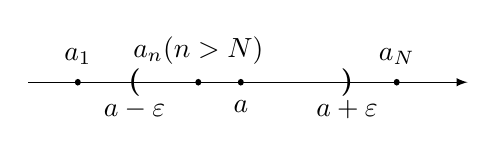
\begin{tikzpicture}[>=latex, xscale=0.9]
  \draw[->] (-3,0) -- (3.2,0);
  \node[above] at (-2.3,0.1) {$a_1$};
  \fill (-2.3,0) circle (1.2pt);
  \node at (-1.5,0) {\textbf{(}};
  \node[below=3pt] at (-1.5,0) {$a-\varepsilon$};
  \node[above] at (-0.6,0.1) {$a_n(n>N)$};
  \fill (-0.6,0) circle (1.2pt);
  \fill (0,0) circle (1.2pt);
  \node[below=3pt] at (0,0) {$a$};
  \node at (1.5,0) {\textbf{)}};
  \node[below=3pt] at (1.5,0) {$a+\varepsilon$};
  \node[above] at (2.2,0.1) {$a_N$};
  \fill (2.2,0) circle (1.2pt);
\end{tikzpicture}
\caption{}\label{fig:1.1.1}
\end{minipage}
\hfill
\begin{minipage}[t]{0.48\textwidth}
\centering
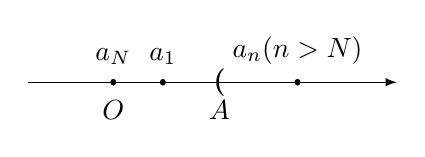
\begin{tikzpicture}[>=latex, xscale=0.9]
  \draw[->] (-1.2,0) -- (4,0);
  \fill (0,0) circle (1.2pt);
  \node[below=3pt] at (0,0) {$O$};
  \node[above] at (0,0.1) {$a_N$};
  \fill (0.7,0) circle (1.2pt);
  \node[above] at (0.7,0.1) {$a_1$};
  \node at (1.5,0) {\textbf{(}};
  \node[below=3pt] at (1.5,0) {$A$};
  \fill (2.6,0) circle (1.2pt);
  \node[above] at (2.6,0.1) {$a_n(n>N)$};
\end{tikzpicture}
\caption{}\label{fig:1.1.2}
\end{minipage}
\end{figure}

如果 $\forall A>0,\ \exists N=N(A)\in\mathbb{N}$, 当 $n>N$ 时, 有 $a_{n}<-A$, 则称 $-\infty$ 为数列 $\{a_{n}\}$ 的极限, 或称 $\{a_{n}\}$ 以 $-\infty$ 为极限, 或 $\{a_{n}\}$ 发散于 $-\infty$, 记为 $\lim_{n\to+\infty}a_{n}=-\infty$ 或 $a_{n}\to-\infty\ (n\to+\infty)$. 此时, 在 $(-\infty,-A)$ 外至多有 $a_{1},\cdots,a_{N}$ 中的 $N$ 项 (如图~\ref{fig:1.1.3} 所示).

如果 $\forall A>0,\ \exists N=N(A)\in\mathbb{N}$, 当 $n>N$ 时, 有
\[
  |a_{n}|>A,
\]
则称 $\infty$ 为数列 $\{a_{n}\}$ 的极限, 或称 $\{a_{n}\}$ 以 $\infty$ 为极限, 或 $\{a_{n}\}$ 发散于 $\infty$, 记为 $\lim_{n\to+\infty}a_{n}=\infty$ 或 $a_{n}\to\infty\ (n\to+\infty)$. 此时, 在 $(-\infty,-A)\cup(A,+\infty)$ 外, 即 $[-A,A]$ 中至多有 $a_{1},\cdots,a_{N}$ 中的 $N$ 项 (如图~\ref{fig:1.1.4} 所示).

\begin{figure}[htbp]
\centering
\begin{minipage}[t]{0.48\textwidth}
\centering
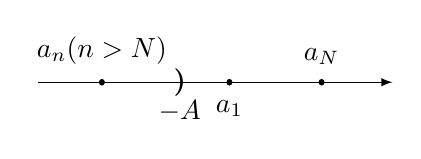
\begin{tikzpicture}[>=latex, xscale=0.9]
  \draw[->] (-3.5,0) -- (1.5,0);
  \fill (-2.6,0) circle (1.2pt);
  \node[above] at (-2.6,0.1) {$a_n(n>N)$};
  \node at (-1.5,0) {\textbf{)}};
  \node[below=3pt] at (-1.5,0) {$-A$};
  \fill (-0.8,0) circle (1.2pt);
  \node[below=3pt] at (-0.8,0) {$a_1$};
  \fill (0.5,0) circle (1.2pt);
  \node[above] at (0.5,0.1) {$a_N$};
\end{tikzpicture}
\caption{}\label{fig:1.1.3}
\end{minipage}
\hfill
\begin{minipage}[t]{0.48\textwidth}
\centering
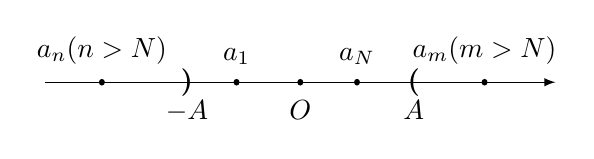
\begin{tikzpicture}[>=latex, xscale=0.9]
  \draw[->] (-3.6,0) -- (3.6,0);
  \fill (-2.8,0) circle (1.2pt);
  \node[above] at (-2.8,0.1) {$a_n(n>N)$};
  \node at (-1.6,0) {\textbf{)}};
  \node[below=3pt] at (-1.6,0) {$-A$};
  \fill (-0.9,0) circle (1.2pt);
  \node[above] at (-0.9,0.1) {$a_1$};
  \fill (0,0) circle (1.2pt);
  \node[below=3pt] at (0,0) {$O$};
  \fill (0.8,0) circle (1.2pt);
  \node[above] at (0.8,0.1) {$a_N$};
  \node at (1.6,0) {\textbf{(}};
  \node[below=3pt] at (1.6,0) {$A$};
  \fill (2.6,0) circle (1.2pt);
  \node[above] at (2.6,0.1) {$a_m(m>N)$};
\end{tikzpicture}
\caption{}\label{fig:1.1.4}
\end{minipage}
\end{figure}

综合上述各种情况可知, 一个数列 $\{a_n\}$ 或者收敛 (即 $\lim_{n\to+\infty}a_n=a\in\mathbb{R}$), 或者发散 (即 $\lim_{n\to+\infty}a_n=+\infty, -\infty, \infty$ 或无极限).

显然, 改变数列 $\{a_{n}\}$ 的有限多项, 或去掉有限多项, 或添加有限多项, 不会改变数列 $\{a_{n}\}$ 的收敛和发散性.

\begin{example}\label{ex:1.1.1}
对常数列 $\{a_{n}\}$, $a_{n} = a$, 有 $\lim_{n \to +\infty} a_{n} = \lim_{n \to +\infty} a = a$.
\end{example}
\begin{proof}
$\forall\varepsilon>0$, 取任意的自然数 $N$, 当 $n>N$ 时, 有
\[
  |a_{n}-a|=|a-a|=0<\varepsilon,
\]
所以 $\lim_{n\to+\infty}a_n=\lim_{n\to+\infty}a=a$.
\end{proof}

\begin{example}\label{ex:1.1.2}
$\lim_{n\to+\infty}\frac{1}{n^\alpha}=0\ (\alpha>0)$.
\end{example}
\begin{proof}
$\forall\varepsilon>0$, 取 $N\in\mathbb{N}$, s.\,t. (such that, 使得) $N>\left(\frac{1}{\varepsilon}\right)^{\frac{1}{\alpha}}$ 或者 $N=\left[\left(\frac{1}{\varepsilon}\right)^{\frac{1}{\alpha}}\right]+1$ (其中 $[x]$ 表示不超过 $x$ 的最大整数), 当 $n>N$ 时, 有
\[
  \left|\frac{1}{n^{\alpha}}-0\right|=\frac{1}{n^{\alpha}}<\frac{1}{N^{\alpha}}<\varepsilon,
\]
所以 $\lim_{n\to+\infty}\frac{1}{n^{\alpha}}=0$.

当 $\alpha=1$ 时, $\lim_{n\to+\infty}\frac{1}{n}=0$, 取 $N=\left[\frac{1}{\varepsilon}\right]+1$ (或 $N>\frac{1}{\varepsilon}, N\in\mathbb{N}$).
\end{proof}

\begin{example}\label{ex:1.1.3}
$\lim_{n\to+\infty}q^n=0\ (|q|<1)$.
\end{example}
\begin{proof}
\textit{证法 1}\quad 当 $0<|q|<1$ 时, $\frac{1}{|q|}>1$, 可设 $\frac{1}{|q|}=1+h\ (h>0)$. $\forall\varepsilon>0$, 取 $N\in\mathbb{N}$, s.\,t. $N>\frac{1}{\varepsilon h}$, 当 $n>N$ 时, 由二项式展开式知
\[
  \frac{1}{|q|^n}=(1+h)^n = 1+nh+\cdots+h^n > nh > Nh > \frac{1}{\varepsilon},
\]
即 $|q^n| < \varepsilon$. 于是
\[
  |q^n-0|=|q^n|<\varepsilon,
\]
所以 $\lim_{n\to+\infty}q^{n}=0$.

当 $q=0$ 时, 由例~\ref{ex:1.1.1} 知, $\lim_{n\to+\infty}q^{n}=\lim_{n\to+\infty}0=0$.

\textit{证法 2}\quad 当 $0<|q|<1$ 时, $\forall\varepsilon>0$, 取 $N\in\mathbb{N}$, s.\,t. $N>\log_{|q|}\varepsilon$, 当 $n>N$ 时, 有
\[
  |q^{n}-0|=|q^{n}|<|q|^{N}<\varepsilon,
\]
所以 $\lim_{n\to+\infty}q^n=0$.
\end{proof}

\begin{example}\label{ex:1.1.4}
证明:
\begin{enumerate}
  \item 当 $q>1$ 时, $\lim_{n\to+\infty}q^n=+\infty$;
  \item 当 $q<-1$ 时, $\lim_{n\to+\infty}q^n=\infty$;
  \item 当 $q=-1$ 时, 数列 $\{q^n\}$ 无极限.
\end{enumerate}
\end{example}
\begin{proof}
(1) 设 $q=1+h\ (h>0)$. $\forall A>0$, 取 $N\in\mathbb{N}$, s.\,t. $N>\frac{A}{h}$. 当 $n>N$ 时, 由二项式定理有
\[
  q^n=(1+h)^n = 1+nh+\cdots+h^n > nh > Nh > A,
\]
所以 $\lim_{n\to+\infty}q^n=+\infty$.

(2) 当 $q<-1$ 时, $|q|>1$. 仿 (1) 可证 $\lim_{n\to+\infty}|q|^n=+\infty$, 即 $\forall A>0,\ \exists N\in\mathbb{N}$, 当 $n>N$ 时, 有 $|q^n|=|q|^n>A$. 因此 $\lim_{n\to+\infty}q^n=\infty$.

(3) 此外, 当 $|q|<1$ 时, 由例~\ref{ex:1.1.3} 知 $\lim_{n\to+\infty}q^n=0$; 当 $q=1$ 时, 由例~\ref{ex:1.1.1} 知 $\lim_{n\to+\infty}q^n=\lim_{n\to+\infty}1=1$; 最后, 当 $q=-1$ 时, 由后面的例~\ref{ex:1.1.12} 推得 $\lim_{n\to+\infty}q^n$ 不存在.
\end{proof}

\begin{example}\label{ex:1.1.5}
设 $a$ 为实常数, 则 $\lim_{n\to+\infty}\frac{a^n}{n!}=0$.
\end{example}
\begin{proof}
显然, $\exists N_{0} \in \mathbb{N}$, s.\,t. $N_{0}>2|a|$, 即 $\frac{|a|}{N_0}<\frac{1}{2}$. 当 $n>N_0$ 时,
\begin{align*}
  \left|\frac{a^{n}}{n!}-0\right| &= \frac{|a|^{n}}{n!} = \frac{|a|}{1}\cdot\frac{|a|}{2}\cdots\frac{|a|}{N_{0}}\cdot\frac{|a|}{N_{0}+1}\cdots\frac{|a|}{n}\\
  &< \frac{|a|^{N_{0}}}{N_{0}!}\left(\frac{|a|}{N_{0}}\right)^{n-N_{0}} < \frac{|a|^{N_{0}}}{N_{0}!}\left(\frac{1}{2}\right)^{n-N_{0}} = C\left(\frac{1}{2}\right)^{n},
\end{align*}
其中 $C = \frac{|a|^{N_0}}{N_0!}\cdot 2^{N_0}$ 为与 $n$ 无关的常数.

由例~\ref{ex:1.1.3} 知, $\lim_{n\to+\infty}\left(\frac{1}{2}\right)^{n}=0$. 故 $\forall\varepsilon>0,\ \exists N_{1}\in\mathbb{N}$, 当 $n>N_1$ 时, 有 $\left(\frac{1}{2}\right)^{n}<\frac{\varepsilon}{C}$. 取 $N=\max\{N_0, N_1\}$, 当 $n>N$ 时, 有
\[
  \left|\frac{a^n}{n!}-0\right| < C\left(\frac{1}{2}\right)^n < C\cdot\frac{\varepsilon}{C}=\varepsilon,
\]
所以 $\lim_{n\to+\infty}\frac{a^n}{n!}=0$.
\end{proof}

\begin{example}\label{ex:1.1.6}
$\lim_{n\to+\infty}\sqrt[n]{a}=\lim_{n\to+\infty}a^{\frac{1}{n}}=1\ (a>0)$.
\end{example}
\begin{proof}
\textit{证法 1}\quad 当 $a=1$ 时, 由例~\ref{ex:1.1.1} 可知 $\lim_{n\to+\infty}\sqrt[n]{a}=\lim_{n\to+\infty}1=1$.

当 $a>1$ 时, $\sqrt[n]{a}>1$. 令 $\sqrt[n]{a}=1+\alpha_n\ (\alpha_n>0)$, 则
\[
  a = (1+\alpha_n)^n = 1+n\alpha_n+\cdots+\alpha_n^n > n\alpha_n,
\]
即 $0<\alpha_n<\frac{a}{n}$. $\forall\varepsilon>0$, 取 $N>\left[\frac{a}{\varepsilon}\right]$, 当 $n>N$ 时, 有
\[
  |\sqrt[n]{a}-1| = \alpha_n < \frac{a}{n} < \frac{a}{N} < \varepsilon,
\]
所以 $\lim_{n\to+\infty}\sqrt[n]{a}=1$.

当 $0<a<1$ 时, $\frac{1}{a}>1$. 由上面已证的结果, $\lim_{n\to+\infty}\sqrt[n]{\frac{1}{a}}=1$, 从而
\[
  \lim_{n\to+\infty}\sqrt[n]{a}=\lim_{n\to+\infty}\frac{1}{\sqrt[n]{\frac{1}{a}}}=1.
\]

\textit{证法 2}\quad 当 $a>1$ 时, $\forall\varepsilon>0$, 只要取 $N\in\mathbb{N}$, s.\,t. $N>\log_{1+\varepsilon}a$, 当 $n>N$ 时, 便有
\[
  1 \leqslant \sqrt[n]{a} < \sqrt[N]{a} < 1+\varepsilon,
\]
即 $|\sqrt[n]{a}-1|<\varepsilon$. 故 $\lim_{n\to+\infty}\sqrt[n]{a}=1$. $a\leqslant 1$ 的情形同证法 1.
\end{proof}

\begin{example}\label{ex:1.1.7}
$\lim_{n\to+\infty}\sqrt[n]{n}=1$.
\end{example}
\begin{proof}
\textit{证法 1}\quad 令 $\sqrt[n]{n}=1+\alpha_{n}\ (\alpha_{n}\geqslant0)$, 则当 $n>1$ 时,
\[
  n = (1+\alpha_{n})^{n} = 1+n\alpha_{n}+\frac{n(n-1)}{2}\alpha_{n}^{2}+\cdots+\alpha_{n}^{n} > \frac{n(n-1)}{2}\alpha_{n}^{2},
\]
从而 $\alpha_n^2 < \frac{2}{n-1}$, 即 $0 \leqslant \alpha_n < \sqrt{\frac{2}{n-1}}$.

$\forall\varepsilon>0$, 取 $N = \left[\frac{2}{\varepsilon^2}\right]+1$, 当 $n>N$ 时, 有
\[
  |\sqrt[n]{n}-1| = \alpha_n < \sqrt{\frac{2}{n-1}} < \sqrt{\frac{2}{N-1}} \leqslant \varepsilon,
\]
所以 $\lim_{n\to+\infty}\sqrt[n]{n}=1$.

\textit{证法 2}\quad $\forall\varepsilon>0$, 取充分大的自然数 $k$, 使 $(1+\varepsilon)^k > 2$. 当 $n>2^k$ 时,
\[
  1 \leqslant \sqrt[n]{n} < \sqrt[n]{(1+\varepsilon)^n} = 1+\varepsilon,
\]
所以 $\lim_{n\to+\infty}\sqrt[n]{n}=1$.
\end{proof}

\begin{example}\label{ex:1.1.8}
设 $a_{n}=0.\underbrace{33\cdots3}_n$, 则 $\lim_{n\to+\infty}a_{n}=\frac{1}{3}$.
\end{example}
\begin{proof}
因为
\[
  a_{n} = \frac{3}{10}+\frac{3}{10^2}+\cdots+\frac{3}{10^n} = \frac{\frac{3}{10}\left(1-\frac{1}{10^n}\right)}{1-\frac{1}{10}} = \frac{1}{3}\left(1-\frac{1}{10^n}\right),
\]
所以
\[
  \left|a_{n}-\frac{1}{3}\right| = \frac{1}{3\cdot 10^n} < \frac{1}{10^n}.
\]
$\forall\varepsilon>0$, 取 $N = \left[\lg\frac{1}{\varepsilon}\right]+1$, 当 $n>N$ 时, 有
\[
  \left|a_{n}-\frac{1}{3}\right| < \frac{1}{10^n} < \frac{1}{10^N} \leqslant \varepsilon,
\]
所以 $\lim_{n\to+\infty}a_{n}=\frac{1}{3}$.
\end{proof}

\begin{example}\label{ex:1.1.9}
$\lim_{n \to +\infty} \frac{1}{n \sqrt[n]{n!}} = 0$.
\end{example}
\begin{proof}
\textit{证法 1}\quad $\forall\varepsilon>0$, 由例~\ref{ex:1.1.5} 知 $\lim_{n\to+\infty}\frac{(1/\varepsilon)^n}{n!}=0$. 故 $\exists N\in\mathbb{N}$, 当 $n>N$ 时, 有
\[
  \frac{(1/\varepsilon)^{n}}{n!}<1,
\]
所以
\[
  -\varepsilon < 0 < \frac{1}{\sqrt[n]{n!}} < \varepsilon,
\]
即 $\lim_{n\to+\infty}\frac{1}{\sqrt[n]{n!}}=0$. 进而由 $n\geqslant 1$ 知
\[
  0 < \frac{1}{n\sqrt[n]{n!}} \leqslant \frac{1}{\sqrt[n]{n!}} < \varepsilon,
\]
所以 $\lim_{n\to+\infty}\frac{1}{n\sqrt[n]{n!}}=0$.

\textit{证法 2}\quad 容易验证不等式 $n! > \left(\frac{n}{e}\right)^n$ (可参阅例~\ref{ex:1.4.11}). 从而
\[
  0 < \frac{1}{n\sqrt[n]{n!}} < \frac{e}{n^2}.
\]
$\forall\varepsilon>0$, 取 $N = \left[\sqrt{\frac{e}{\varepsilon}}\right]+1$, 当 $n>N$ 时即有 $\frac{e}{n^2}<\varepsilon$, 故极限为 0.
\end{proof}

\begin{example}\label{ex:1.1.10}
$\lim_{n\to+\infty}\frac{3n^{2}}{n^{2}-3}=3$.
\end{example}
\begin{proof}
当 $n\geqslant 2$ 时, $n^2-3 > \frac{n^2}{2}$. 故
\[
  \left|\frac{3n^{2}}{n^{2}-3}-3\right| = \frac{9}{n^{2}-3} < \frac{18}{n^{2}}.
\]
$\forall\varepsilon>0$, 取 $N = \max\left\{2, \left[\sqrt{\frac{18}{\varepsilon}}\right]+1\right\}$, 当 $n>N$ 时, 有
\[
  \left|\frac{3n^{2}}{n^{2}-3}-3\right| < \frac{18}{n^2} < \frac{18}{N^2} \leqslant \varepsilon,
\]
所以 $\lim_{n\to+\infty}\frac{3n^{2}}{n^{2}-3}=3$.
\end{proof}

\begin{example}\label{ex:1.1.11}
$\lim_{n \to +\infty} \frac{3 \sqrt{n} + 1}{2 \sqrt{n} + n} = 0$.
\end{example}
\begin{proof}
$\forall\varepsilon>0$, 当 $n\geqslant 1$ 时,
\[
  \left|\frac{3\sqrt{n}+1}{2\sqrt{n}+n}-0\right| = \frac{3\sqrt{n}+1}{2\sqrt{n}+n} < \frac{4\sqrt{n}}{n} = \frac{4}{\sqrt{n}}.
\]
取 $N = \left[\frac{16}{\varepsilon^2}\right]+1$, 当 $n>N$ 时, 有
\[
  \left|\frac{3\sqrt{n}+1}{2\sqrt{n}+n}-0\right| < \frac{4}{\sqrt{n}} < \frac{4}{\sqrt{N}} \leqslant \varepsilon,
\]
所以 $\lim_{n\to+\infty}\frac{3\sqrt{n}+1}{2\sqrt{n}+n}=0$.
\end{proof}

\begin{theorem}\label{thm:1.1.1}
数列 $\{a_{n}\}$ 有极限 $a$ 的充分必要条件是它的偶数项数列 (偶子列) $\{a_{2k}\}$ 和奇数项数列 (奇子列) $\{a_{2k-1}\}$ 都有极限且极限均为 $a$.
\end{theorem}
\begin{proof}
\textbf{必要性:}\quad 设 $\lim_{n\to+\infty}a_n=a$.

若 $a$ 为有限实数, 则 $\forall\varepsilon>0,\ \exists N\in\mathbb{N}$, 当 $n>N$ 时, 有 $|a_n-a|<\varepsilon$. 特别地, 取自然数 $K = \left[\frac{N}{2}\right]+1$, 当 $k>K$ 时, $2k>2k-1>N$, 因而
\[
  |a_{2k}-a|<\varepsilon\quad \text{与}\quad |a_{2k-1}-a|<\varepsilon,
\]
即 $\lim_{k\to+\infty}a_{2k}=a$ 且 $\lim_{k\to+\infty}a_{2k-1}=a$.

对 $a=+\infty, -\infty, \infty$ 的情形完全类似可证.

\textbf{充分性:}\quad 设 $\lim_{k\to+\infty}a_{2k}=a$ 且 $\lim_{k\to+\infty}a_{2k-1}=a$.

若 $a$ 为有限实数, 则 $\forall\varepsilon>0$, $\exists K_1\in\mathbb{N}$, 当 $k>K_1$ 时, $|a_{2k}-a|<\varepsilon$; $\exists K_2\in\mathbb{N}$, 当 $k>K_2$ 时, $|a_{2k-1}-a|<\varepsilon$. 取 $N = \max\{2K_1, 2K_2-1\}$, 则当 $n>N$ 时, 无论 $n$ 是偶数 ($n=2k>2K_1$) 还是奇数 ($n=2k-1>2K_2-1$), 都有 $|a_n-a|<\varepsilon$. 故 $\lim_{n\to+\infty}a_n=a$.

对 $a=+\infty, -\infty, \infty$ 的情形同理可证.
\end{proof}

下面引进开邻域的概念:
\begin{enumerate}
  \item 设 $a\in\mathbb{R}$, 称开区间 $(a-\varepsilon, a+\varepsilon)$ 为点 $a$ 的 $\varepsilon$ 邻域, 记作 $U(a;\varepsilon)$ 或简记为 $U(a)$. 称集合 $U^\circ(a;\varepsilon) = (a-\varepsilon, a)\cup(a, a+\varepsilon)$ 为点 $a$ 的去心邻域.
  \item 称开区间 $(A, +\infty)$ 为点 $+\infty$ 的开邻域, 记作 $U(+\infty; A)$ 或 $U(+\infty)$.
  \item 称开区间 $(-\infty, -A)$ 为点 $-\infty$ 的开邻域, 记作 $U(-\infty; A)$ 或 $U(-\infty)$.
  \item 称开集 $(-\infty, -A)\cup(A, +\infty)$ 为点 $\infty$ 的开邻域, 记作 $U(\infty; A)$ 或 $U(\infty)$.
\end{enumerate}

由开邻域的概念, 数列极限的定义可以统一叙述为:
\[
  \lim_{n\to+\infty}a_n = a \iff \text{对 } a \text{ 的任何开邻域 } U,\ \exists N\in\mathbb{N},\ \text{当 } n>N \text{ 时, } a_n\in U.
\]

\begin{theorem}\label{thm:1.1.2}
$\lim_{n\to+\infty}a_n=a \iff$ 对 $\{a_n\}$ 的任何子列 $\{a_{n_k}\}$ 都有 $\lim_{k\to+\infty}a_{n_k}=a$.
\end{theorem}
\begin{proof}
\textbf{充分性:}\quad 因为数列 $\{a_n\}$ 本身就是它的一个平凡子列 (取 $n_k=k$), 所以结论显然成立.

\textbf{必要性:}\quad 设 $\lim_{n\to+\infty}a_n=a$. 对 $a$ 的任何开邻域 $U$, $\exists N\in\mathbb{N}$, 当 $n>N$ 时, $a_n\in U$. 因为子列的下标序列 $\{n_k\}$ 严格递增, 且 $n_k\geqslant k$, 所以当 $k>N$ 时必有 $n_k\geqslant k>N$, 从而 $a_{n_k}\in U$. 故 $\lim_{k\to+\infty}a_{n_k}=a$.
\end{proof}

\begin{theorem}\label{thm:1.1.3}
数列 $\{a_{n}\}$ 有极限 (实数 $a$ 或 $+\infty$ 或 $-\infty$) 的充要条件是它的任何非平凡子列都有极限.
\end{theorem}
\begin{proof}
必要性由定理~\ref{thm:1.1.2} 直接保证. 充分性反设 $\{a_n\}$ 没有极限, 则由极限否定定义可析出两个极限不同的子列, 矛盾.
\end{proof}

\begin{theorem}\label{thm:1.1.4}
数列 $\{a_{n}\}$ 收敛 $\iff \{a_{n}\}$ 的任何非平凡子列都收敛.
\end{theorem}

\begin{theorem}\label{thm:1.1.5}
$\lim_{n \to +\infty} a_n = a \iff a$ 的任何开邻域 $U$ 的外边 $\mathbb{R} \setminus U$ 中至多含有限项.
\end{theorem}
\begin{proof}
\textbf{必要性:}\quad 由极限定义, 当 $n>N$ 时 $a_n\in U$, 故在 $U$ 外部至多只有 $a_1, a_2, \cdots, a_N$ 这有限多项.

\textbf{充分性:}\quad 对任何开邻域 $U$, 若 $U$ 外面只有有限项, 设这些项的最大下标为 $N$ (若外面无项则取 $N=1$), 则当 $n>N$ 时必有 $a_n\in U$, 从而 $\lim_{n\to+\infty}a_n=a$.
\end{proof}

\begin{example}\label{ex:1.1.12}
数列 $\{a_{n}\}$, $a_{n} = (-1)^{n-1}$ 无极限, 当然不收敛.
\end{example}
\begin{proof}
\textit{证法 1}\quad 它的奇子列 $a_{2k-1} = 1 \to 1$, 偶子列 $a_{2k} = -1 \to -1$. 由定理~\ref{thm:1.1.1} 或定理~\ref{thm:1.1.2} 知, $(-1)^{n-1}$ 无极限.

\textit{证法 2}\quad $\forall a\neq\pm 1$, 取 $\varepsilon_{0}=\min\{|a-1|, |a+1|\}>0$, 则数列 $(-1)^{n-1}$ 全部各项都在开邻域 $U=(a-\varepsilon_0, a+\varepsilon_0)$ 的外部.
当 $a=1$ 时, $-1=(-1)^{2k}$ 全在 $1$ 的开邻域 $U=(1-1/2, 1+1/2)=(1/2, 3/2)$ 外部;
当 $a=-1$ 时, $1=(-1)^{2k-1}$ 全在 $-1$ 的开邻域 $U=(-3/2, -1/2)$ 外部;
当 $a=+\infty$ 时, 全在 $U=(1, +\infty)$ 外部;
当 $a=-\infty$ 时, 全在 $U=(-\infty, -1)$ 外部;
当 $a=\infty$ 时, 全在 $U=(-\infty, -1)\cup(1, +\infty)$ 外部.
根据定理~\ref{thm:1.1.5}, 任何数及 $\pm\infty, \infty$ 均不为该数列极限.
\end{proof}

\begin{example}\label{ex:1.1.13}
数列 $\{\sin n\}$ 无极限.
\end{example}
\begin{proof}
$\forall k\in\mathbb{N}$, 区间 $\left(2k\pi+\frac{\pi}{4}, 2k\pi+\frac{3\pi}{4}\right)$ 的长度为 $\frac{\pi}{2}>1$, 故必存在自然数 $n_{k}\in\left(2k\pi+\frac{\pi}{4}, 2k\pi+\frac{3\pi}{4}\right)\cap\mathbb{N}$. 同理, 区间 $((2k-1)\pi, 2k\pi)$ 的长度为 $\pi>1$, 必存在自然数 $n_{k}'\in((2k-1)\pi, 2k\pi)\cap\mathbb{N}$ (如图~\ref{fig:1.1.5} 所示).

\begin{figure}[htbp]
\centering
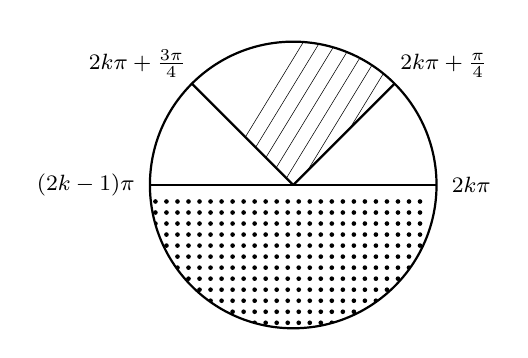
\begin{tikzpicture}[>=latex, scale=1.4]
  % 扇形斜线阴影
  \begin{scope}
    \clip (0,0) -- (45:1.3) arc (45:135:1.3) -- cycle;
    \foreach \x in {-1.8,-1.65,...,1.8} {
      \draw[very thin] (\x,-1.8) -- (\x+2.2,1.8);
    }
  \end{scope}
  % 下半圆点阵阴影
  \begin{scope}
    \clip (-1.3,0) arc (180:360:1.3) -- cycle;
    \foreach \x in {-1.25,-1.15,...,1.25} {
      \foreach \y in {-1.25,-1.15,...,-0.05} {
        \fill (\x,\y) circle (0.6pt);
      }
    }
  \end{scope}
  % 轮廓与分割线
  \draw[thick] (0,0) circle (1.3);
  \draw[thick] (-1.3,0) -- (1.3,0);
  \draw[thick] (0,0) -- (45:1.3);
  \draw[thick] (0,0) -- (135:1.3);
  % 标注
  \node[left=2pt] at (-1.3,0) {\footnotesize $(2k-1)\pi$};
  \node[right=2pt] at (1.3,0) {\footnotesize $2k\pi$};
  \node[above left] at (135:1.25) {\footnotesize $2k\pi+\frac{3\pi}{4}$};
  \node[above right] at (45:1.25) {\footnotesize $2k\pi+\frac{\pi}{4}$};
\end{tikzpicture}
\caption{}\label{fig:1.1.5}
\end{figure}

显然 $n_1<n_2<\cdots$ 且 $n_1'<n_2'<\cdots$. 对于子列 $\{a_{n_k}\}$, 有
\[
  a_{n_k} = \sin n_k > \sin\frac{\pi}{4} = \frac{\sqrt{2}}{2};
\]
而对于子列 $\{a_{n_k'}\}$, 有
\[
  a_{n_k'} = \sin n_k' < 0.
\]
故若极限存在为 $a$, 则必然有 $a\geqslant\frac{\sqrt{2}}{2}$ 且 $a\leqslant 0$, 矛盾! 故数列 $\{\sin n\}$ 无极限.
\end{proof}

\begin{theorem}[保号性与保序性]\label{thm:1.1.6}
设 $\lim_{n\to+\infty} a_n = a > b$ (或 $<b$), 则 $\exists N_0 \in \mathbb{N}$, 当 $n>N_0$ 时有 $a_n > b$ (或 $a_n < b$).
\end{theorem}
\begin{proof}
取 $\varepsilon = a-b > 0$. 由极限定义, $\exists N_0\in\mathbb{N}$, 当 $n>N_0$ 时, 有
\[
  |a_n-a| < \varepsilon \implies a_n > a-\varepsilon = a-(a-b) = b.
\]
同理可证 $a<b$ 的情形.
\end{proof}

\begin{example}\label{ex:1.1.14}
设 $\lim_{n\to+\infty}a_n=0$ (极限为 0 的变量称为无穷小量), 且数列 $\{b_n\}$ 有界 (即 $\exists M>0$ 使 $|b_n|\leqslant M$), 则
\[
  \lim_{n\to+\infty}a_n b_n = 0.
\]
即无穷小量与有界变量之积仍为无穷小量.
\end{example}
\begin{proof}
$\forall\varepsilon>0$, 因 $\lim_{n\to+\infty}a_n=0$, 故 $\exists N\in\mathbb{N}$, 当 $n>N$ 时, 有 $|a_n-0|<\frac{\varepsilon}{M+1}$. 于是
\[
  |a_{n}b_{n}-0|=|a_{n}b_{n}|\leqslant M|a_{n}| \leqslant M\cdot\frac{\varepsilon}{M+1}<\varepsilon,
\]
所以 $\lim_{n\to+\infty}a_n b_n = 0$.
\end{proof}

\begin{example}[Ces\`aro 算术平均]\label{ex:1.1.15}
设 $\lim_{n\to+\infty}a_n=a$ (实数, $+\infty, -\infty$), 则
\[
  \lim_{n\to+\infty}\frac{a_1+a_2+\cdots+a_n}{n}=a.
\]
但反之不真.
\end{example}
\begin{proof}
反之不真显见: 取 $a_n=(-1)^{n-1}$, 则 $\{a_n\}$ 发散, 但 $\frac{a_1+\cdots+a_n}{n}\to 0$.

现在证明正向结论:
当 $a\in\mathbb{R}$ 时, 设 $a_n = a+\alpha_n$, 其中 $\lim_{n\to+\infty}\alpha_n=0$. 则
\[
  \frac{a_1+\cdots+a_n}{n} = a + \frac{\alpha_1+\cdots+\alpha_n}{n}.
\]
$\forall\varepsilon>0$, $\exists N_1\in\mathbb{N}$, 当 $n>N_1$ 时, $|\alpha_n|<\frac{\varepsilon}{2}$. 取定 $N_1$ 后, $\sum_{k=1}^{N_1}|\alpha_k|$ 为常数, 故 $\exists N_2>N_1$, 当 $n>N_2$ 时, $\frac{\sum_{k=1}^{N_1}|\alpha_k|}{n}<\frac{\varepsilon}{2}$. 于是当 $n>N_2$ 时,
\[
  \left|\frac{\alpha_1+\cdots+\alpha_n}{n}\right| \leqslant \frac{\sum_{k=1}^{N_1}|\alpha_k|}{n} + \frac{\sum_{k=N_1+1}^n|\alpha_k|}{n} < \frac{\varepsilon}{2} + \frac{(n-N_1)\frac{\varepsilon}{2}}{n} < \varepsilon.
\]
故 $\lim_{n\to+\infty}\frac{a_1+\cdots+a_n}{n}=a$.

当 $a=+\infty$ 时, $\forall A>0$, $\exists N_1\in\mathbb{N}$, 当 $n>N_1$ 时, $a_n > 2A+2$. 固定 $N_1$, 因 $\lim_{n\to+\infty}\frac{n-N_1}{n}=1>\frac{1}{2}$ 且 $\lim_{n\to+\infty}\frac{a_1+\cdots+a_{N_1}}{n}=0>-1$, 故 $\exists N_2>N_1$, 当 $n>N_2$ 时, 有
\[
  \frac{a_1+\cdots+a_n}{n} = \frac{a_1+\cdots+a_{N_1}}{n} + \frac{a_{N_1+1}+\cdots+a_n}{n} > -1 + \frac{n-N_1}{n}(2A+2) > -1 + \frac{1}{2}(2A+2) = A.
\]
故 $\lim_{n\to+\infty}\frac{a_1+\cdots+a_n}{n}=+\infty$.

$a=-\infty$ 的情形完全类似可证.
\end{proof}

\begin{example}\label{ex:1.1.16}
数列 $\{a_{n}\}$ 无上界 $\iff \{a_{n}\}$ 必有子列 $\{a_{n_{k}}\}$ 使得 $\lim_{k\to+\infty}a_{n_k}=+\infty$.
\end{example}
\begin{proof}
\textbf{充分性:}\quad 若有子列 $a_{n_k}\to+\infty$, 则对任意 $M>0$, 存在 $K$ 使得当 $k>K$ 时 $a_{n_k}>M$, 故原数列无上界.

\textbf{必要性:}\quad 设 $\{a_n\}$ 无上界. 取 $k=1$, $\exists n_1\in\mathbb{N}$ 使 $a_{n_1}>1$.
假设已选出 $n_1<n_2<\cdots<n_{k-1}$ 满足 $a_{n_j}>j\ (j=1,\cdots,k-1)$. 令
\[
  M_k = \max\{k, a_1, a_2, \cdots, a_{n_{k-1}}\}.
\]
因为 $\{a_n\}$ 无上界, 故必存在 $n_k$ 使得 $a_{n_k}>M_k$. 显然 $a_{n_k}>k$, 且由 $a_{n_k}>M_k \geqslant a_i\ (1\leqslant i\leqslant n_{k-1})$ 可知 $n_k > n_{k-1}$.
以此归纳可得子列 $\{a_{n_k}\}$, 满足 $n_1<n_2<\cdots$ 且 $a_{n_k}>k$. 故 $\lim_{k\to+\infty}a_{n_k}=+\infty$.
\end{proof}

\begin{exblock}{练习题 1.1}
\item 用数列极限定义证明:
\begin{enumerate}
  \item $\lim_{n \to +\infty} 0.\underbrace{99 \cdots 9}_n = 1$;
  \item $\lim_{n \to +\infty} \frac{3n + 4}{7n - 3} = \frac{3}{7}$;
  \item $\lim_{n \to +\infty} \frac{5n + 6}{n^2 - n - 1000} = 0$;
  \item $\lim_{n \to +\infty} \frac{8}{2^n + 5} = 0$;
  \item $\lim_{n \to +\infty} \frac{\sin n!}{n^{1/2}} = 0$;
  \item $\lim_{n \to +\infty} (\sqrt{n + 2} - \sqrt{n - 2}) = 0$;
  \item $\lim_{n \to +\infty} (\sqrt[3]{n+2} - \sqrt[3]{n-2}) = 0$;
  \item $\lim_{n \to +\infty} \frac{n^{3/2} \arctan n}{1 + n^2} = 0$;
  \item $\lim_{n \to +\infty} a_n = 1$, 其中 $a_n = \begin{cases} \frac{n-1}{n}, & n \text{ 为偶数}, \\ \frac{\sqrt{n^2 + n}}{n}, & n \text{ 为奇数}; \end{cases}$
  \item $\lim_{n \to +\infty} (n^3 - 4n - 5) = +\infty$.
\end{enumerate}

\item 设 $\lim_{n\to+\infty}a_n=a$. 证明: $\forall k\in\mathbb{N}$, 有 $\lim_{n\to+\infty}a_{n+k}=a$.

\item 设 $\lim_{n\to+\infty}a_n=a$. 证明: $\lim_{n\to+\infty}|a_n|=|a|$. 举例说明, 这个命题的逆命题不真.

\item 设 $x_{n} \leqslant a \leqslant y_{n}, n \in \mathbb{N}$, 且 $\lim_{n\to+\infty}(y_{n}-x_{n})=0$. 证明:
\[
  \lim_{n\to+\infty}x_{n}=\lim_{n\to+\infty}y_{n}=a.
\]

\item 设 $\{a_{n}\}$ 为一个收敛数列. 证明: 数列 $\{a_{n}\}$ 中或者有最大的数, 或者有最小的数. 举出两者都有的例子; 再举出只有一个的例子.

\item 证明下列数列发散:
\begin{enumerate}
  \item $\{n^{(-1)^n}\}$;
  \item $\{\cos n\}$.
\end{enumerate}

\item 证明: 数列 $\{a_{n}\}$ 收敛 $\iff$ 三个数列 $\{a_{3k-2}\}$, $\{a_{3k-1}\}$, $\{a_{3k}\}$ 都收敛且有相同的极限.

\item 设 $\lim_{n\to+\infty}(a_{n}-a_{n-1})=d$. 证明: $\lim_{n\to+\infty}\frac{a_n}{n}=d$.

\item 设 $\lim_{n\to+\infty} a_n = a$. 用 $\varepsilon\text{-}N$ 法, $A\text{-}N$ 法证明:
\[
  \lim_{n\to+\infty}\frac{a_1+2a_2+\cdots+na_n}{n^2}=\frac{a}{2}\quad (a \text{ 为实数}, +\infty, -\infty).
\]
\end{exblock}

\begin{exblock}{思考题 1.1}
\item 设 $\lim_{n\to+\infty}a_n=a$, $|q| < 1$. 用 $\varepsilon\text{-}N$ 法证明:
\[
  \lim_{n\to+\infty}(a_{n}+a_{n-1}q+\cdots+a_{1}q^{n-1})=\frac{a}{1-q}.
\]

\item 设 $\lim_{n\to+\infty}a_n=a$, $\lim_{n\to+\infty}b_n=b$. 用 $\varepsilon\text{-}N$ 法证明:
\[
  \lim_{n\to+\infty}\frac{a_0b_n+a_1b_{n-1}+\cdots+a_{n-1}b_1+a_nb_0}{n}=ab.
\]

\item 设 $\lim_{n\to+\infty}a_n=a, b_n\geqslant 0\ (n\in\mathbb{N}), \lim_{n\to+\infty}(b_1+b_2+\cdots+b_n)=S$. 证明:
\[
  \lim_{n\to+\infty}(a_nb_1+a_{n-1}b_2+\cdots+a_1b_n)=aS.
\]

\item \textbf{(Toeplitz 定理)}\ 设 $n, k \in \mathbb{N}$, $t_{nk} \geqslant 0$ 且 $\sum_{k=1}^{n} t_{nk} = 1$, $\lim_{n \to +\infty} t_{nk} = 0$. 如果 $\lim_{n \to +\infty} a_n = a$, 证明:
\[
  \lim_{n \to +\infty} \sum_{k=1}^{n} t_{nk} a_k = a.
\]
说明例~\ref{ex:1.1.15} 为 Toeplitz 定理的特殊情形.

\item 设 $a, b, c$ 为三个给定的实数, 令 $a_{0} = a, b_{0} = b, c_{0} = c$, 并归纳定义
\[
  \begin{cases}
    a_{n}=\dfrac{b_{n-1}+c_{n-1}}{2},\\[6pt]
    b_{n}=\dfrac{c_{n-1}+a_{n-1}}{2}, & n = 1, 2, \cdots.\\[6pt]
    c_{n}=\dfrac{a_{n-1}+b_{n-1}}{2},
\end{cases}
\]
证明: $\lim_{n\to+\infty}a_n=\lim_{n\to+\infty}b_n=\lim_{n\to+\infty}c_n=\frac{a+b+c}{3}$.

\item 设 $a_{1}, a_{2}$ 为实数, 令
\[
  a_{n}=pa_{n-1}+qa_{n-2},\quad n=3, 4, 5, \cdots,
\]
其中 $p > 0, q > 0, p + q = 1$. 证明: 数列 $\{a_{n}\}$ 收敛, 且 $\lim_{n \to +\infty} a_{n} = \frac{a_{2} + a_{1} q}{1 + q}$.

\item 设数列 $\{a_{n}\}$, $\{b_{n}\}$, $\{c_{n}\}$ 满足 $a_{1} > 0, 4 \leqslant b_{n} \leqslant 5, 4 \leqslant c_{n} \leqslant 5$,
\[
  a_{n}=\frac{\sqrt{b_{n}^{2}+c_{n}^{2}}}{b_{n}+c_{n}}a_{n-1}.
\]
证明: $\lim_{n\to+\infty}a_n = 0$.
\end{exblock}

\section{数列极限的基本性质}\label{sec:1.2}

在定义了数列极限之后，我们会用 $\varepsilon\text{-}N$ 法证明一些数列的极限，但从上节知道，这必须在已知数列有无极限的前提下才能应用，且某些证明还相当复杂，有些甚至还无法用 $\varepsilon\text{-}N$ 法证明。所以，我们必须进一步了解数列极限有哪些性质，还有什么方法可以使用。为此，本节将逐一给出数列极限的唯一性，收敛数列的有界性，极限的四则运算性质，不等式性质以及重要的夹逼定理。

\begin{theorem}[极限的惟一性]\label{thm:1.2.1}
设数列 $\{a_{n}\}$ 有极限（实数，或 $+\infty$，或 $-\infty$），则极限是惟一的。
\end{theorem}

\begin{proof}
\textbf{证法 1} 设 $\lim\limits_{n\to+\infty}a_n=a$ 及 $\lim\limits_{n\to+\infty}a_n=b$，$a,b\in\mathbb{R}$。

（反证）反设 $a \neq b$。令 $\varepsilon_{0} = |a - b| > 0$，根据数列极限的定义~\ref{def:1.1.1}，$\exists N \in \mathbb{N}$，当 $n > N$ 时，
\[
|a_{n}-a|<\frac{\varepsilon_{0}}{2},\quad |a_{n}-b|<\frac{\varepsilon_{0}}{2},
\]
所以，
\[
|a-b| \leqslant |a-a_{n}| + |a_{n}-b| < \frac{\varepsilon_{0}}{2} + \frac{\varepsilon_{0}}{2} = \varepsilon_{0} = |a-b|,
\]
矛盾。

值得注意的是这种证法不能应用到极限为 $+\infty$ 或 $-\infty$ 的情况，因此还必须给出能推广到 $+\infty$ 或 $-\infty$ 的证法，于是有下面证法。

\textbf{证法 2} 设 $\lim\limits_{n\to+\infty}a_n=a$ 及 $\lim\limits_{n\to+\infty}a_n=b$，$a,b\in\mathbb{R}$。

（反证）反设 $a \neq b$，不失一般性，设 $a < b$。令 $\varepsilon_{0} = \frac{b - a}{2} > 0$。由极限定义~\ref{def:1.1.1} 知，$\exists N_{1} \in \mathbb{N}$，当 $n > N_{1}$ 时，$a - \varepsilon_{0} < a_{n} < a + \varepsilon_{0}$；$\exists N_{2} \in \mathbb{N}$，当 $n > N_{2}$ 时，$b - \varepsilon_{0} < a_{n} < b + \varepsilon_{0}$。所以，当 $n > N = \max\{N_{1}, N_{2}\}$ 时，
\[
\frac{a+b}{2} = b - \frac{b-a}{2} = b - \varepsilon_{0} < a + \varepsilon_{0} = a + \frac{b-a}{2} = \frac{a+b}{2},
\]
矛盾。

其他情形类似证明。

\textbf{证法 3}（统一描述）设 $\lim\limits_{n\to+\infty}a_n=a$ 及 $\lim\limits_{n\to+\infty}a_n=b$。

（反证）反设 $a \neq b$，不妨设 $a < b$，则存在 $a$ 的开邻域 $U_a$ 与 $b$ 的开邻域 $U_b$，使得 $U_a \cap U_b = \varnothing$。由极限定义~\ref{def:1.1.1} 知，$\exists N_1 \in \mathbb{N}$，当 $n > N_1$ 时，$a_n \in U_a$；$\exists N_2 \in \mathbb{N}$，当 $n > N_2$ 时，$a_n \in U_b$。所以，当 $n > \max\{N_1, N_2\}$ 时，$a_n \in U_a \cap U_b = \varnothing$，矛盾。
\end{proof}

\begin{definition}\label{def:1.2.1}
如果存在实数 $M>0$，使得对任何自然数 $n$，有 $|a_{n}| \leqslant M$，则称数列 $\{a_{n}\}$ \textbf{有界}。如果存在实数 $B$，使得 $a_{n} \leqslant B$（$\forall n \in \mathbb{N}$），则称数列 $\{a_{n}\}$ \textbf{有上界} $B$。如果存在实数 $A$，使得 $a_{n} \geqslant A$（$\forall n \in \mathbb{N}$），则称数列 $\{a_{n}\}$ \textbf{有下界} $A$。
\end{definition}

显然，$\{a_{n}\}$ 有界的充要条件是 $\{a_{n}\}$ 既有上界又有下界。

\begin{theorem}\label{thm:1.2.2}
数列 $\{a_{n}\}$ 收敛，则 $\{a_{n}\}$ 必有界。反之不真。
\end{theorem}

\begin{proof}
设 $\lim\limits_{n \to \infty} a_n = a \in \mathbb{R}$。取 $\varepsilon_0 = 1$，$\exists N_0 \in \mathbb{N}$，当 $n > N_0$ 时，$|a_n - a| < \varepsilon_0 = 1$，所以，
\[
|a_{n}| = |(a_{n}-a)+a| \leqslant |a_{n}-a| + |a| < 1 + |a|.
\]
于是，$\forall n \in \mathbb{N}$，有
\[
|a_{n}| \leqslant \max\{|a_{1}|, \cdots, |a_{N_{0}}|, |a|+1\} = M,
\]
即数列 $\{a_{n}\}$ 有界。

反之则有反例 $a_{n}=(-1)^{n-1}$，满足 $|a_{n}| \leqslant 1$，有界。但由例 1.1.12 已知，$a_{n}=(-1)^{n-1}$ 时数列发散。
\end{proof}

\begin{theorem}[极限的四则运算]\label{thm:1.2.3}
设 $\{a_{n}\}, \{b_{n}\}$ 都收敛，则 $\{a_{n}\pm b_{n}\}, \{a_{n}b_{n}\}$ 也收敛。又若 $\lim\limits_{n\to+\infty}b_{n}\neq0$，则 $\left\{\frac{a_{n}}{b_{n}}\right\}$ 也收敛。且
\begin{enumerate}
  \item $\lim\limits_{n \to +\infty} (a_n \pm b_n) = \lim\limits_{n \to +\infty} a_n \pm \lim\limits_{n \to +\infty} b_n$；
  \item $\lim\limits_{n\to+\infty} a_n b_n = \lim\limits_{n\to+\infty} a_n \cdot \lim\limits_{n\to+\infty} b_n$，特别有 $\lim\limits_{n\to+\infty} c a_n = c \lim\limits_{n\to+\infty} a_n$；
  \item $\lim\limits_{n \to +\infty} \frac{a_n}{b_n} = \frac{\lim\limits_{n \to +\infty} a_n}{\lim\limits_{n \to +\infty} b_n}\ (\lim\limits_{n \to +\infty} b_n \neq 0)$。
\end{enumerate}
\end{theorem}

\begin{proof}
(1) $\forall \varepsilon > 0$，因 $\lim\limits_{n \to +\infty} a_n = a \in \mathbb{R}$，$\lim\limits_{n \to +\infty} b_n = b \in \mathbb{R}$，所以，$\exists N_1 \in \mathbb{N}$，当 $n > N_1$ 时，$|a_n - a| < \frac{\varepsilon}{2}$；$\exists N_2 \in \mathbb{N}$，当 $n > N_2$ 时，$|b_n - b| < \frac{\varepsilon}{2}$。于是，当 $n > N = \max\{N_1, N_2\}$ 时，
\begin{align*}
|(a_{n}\pm b_{n})-(a\pm b)| &= |(a_{n}-a)\pm(b_{n}-b)| \\
&\leqslant |a_{n}-a| + |b_{n}-b| \\
&< \frac{\varepsilon}{2} + \frac{\varepsilon}{2} = \varepsilon,
\end{align*}
由此就有 $\lim\limits_{n\to+\infty}(a_n\pm b_n) = a\pm b = \lim\limits_{n\to+\infty}a_n \pm \lim\limits_{n\to+\infty}b_n$。

(2) 因为 $\lim\limits_{n \to +\infty} b_n = b \in \mathbb{R}$，由定理~\ref{thm:1.2.2} 可知，$|b_n| < M$（$\forall n \in \mathbb{N}$）。又因 $\lim\limits_{n \to +\infty} a_n = a \in \mathbb{R}$，故 $\forall \varepsilon > 0$，$\exists N \in \mathbb{N}$，当 $n > N$ 时，
\[
|a_{n}-a| < \frac{\varepsilon}{2M},\quad |b_{n}-b| < \frac{\varepsilon}{2(|a|+1)},
\]
及
\begin{align*}
|a_{n}b_{n}-ab| &= |a_{n}b_{n}-ab_{n}+ab_{n}-ab| \leqslant |b_{n}||a_{n}-a| + |a||b_{n}-b| \\
&< M \frac{\varepsilon}{2M} + |a| \frac{\varepsilon}{2(|a|+1)} < \frac{\varepsilon}{2} + \frac{\varepsilon}{2} = \varepsilon.
\end{align*}
这就证明了
\[
\lim_{n\to+\infty}a_nb_n = ab = \lim_{n\to+\infty}a_n \cdot \lim_{n\to+\infty}b_n.
\]

(3) 先证：如果 $\lim\limits_{n\to+\infty}b_n=b\neq0$，则 $\lim\limits_{n\to+\infty}\frac{1}{b_n}=\frac{1}{b}$。事实上，$\forall\varepsilon>0$，$\exists N\in\mathbb{N}$，当 $n>N$ 时，
\[
|b_{n}-b| < \min\left\{\frac{|b|}{2}, \frac{b^{2}}{2}\varepsilon\right\}.
\]
则当 $n > N$ 时，有
\[
|b_{n}| = |(b_{n}-b)+b| \geqslant |b| - |b_{n}-b| > |b| - \frac{|b|}{2} = \frac{|b|}{2},
\]
\[
\left|\frac{1}{b_{n}}-\frac{1}{b}\right| = \frac{|b_{n}-b|}{|b_{n}||b|} < \frac{|b_{n}-b|}{\frac{|b|}{2}|b|} < \frac{2}{b^{2}} \cdot \frac{b^{2}}{2}\varepsilon = \varepsilon.
\]
这就证明了
\[
\lim_{n\to+\infty}\frac{1}{b_{n}} = \frac{1}{b}.
\]
由此得到
\[
\lim_{n\to+\infty}\frac{a_{n}}{b_{n}} = \lim_{n\to+\infty}a_{n} \cdot \frac{1}{b_{n}} = a \cdot \frac{1}{b} = \frac{a}{b} = \frac{\lim\limits_{n\to+\infty}a_{n}}{\lim\limits_{n\to+\infty}b_{n}}.
\]
\end{proof}

\begin{theorem}\label{thm:1.2.4}
设 $\lim\limits_{n\to+\infty}a_n=a$，$\lim\limits_{n\to+\infty}b_n=b$，$a<b$。则存在自然数 $N_0$，当 $n>N_0$ 时，有 $a_n<b_n$。
\end{theorem}

\begin{proof}
\textbf{证法 1} 当 $a, b \in \mathbb{R}$ 时，令 $\varepsilon_{0} = \frac{b - a}{2} > 0$。因 $\lim\limits_{n \to +\infty} a_{n} = a$，$\lim\limits_{n \to +\infty} b_{n} = b$，则存在自然数 $N_{0}$，当 $n > N_{0}$ 时，有
\[
\frac{3a-b}{2} = a - \frac{b-a}{2} < a_{n} < a + \frac{b-a}{2} = \frac{a+b}{2},
\]
\[
\frac{a+b}{2} = b - \frac{b-a}{2} < b_{n} < b + \frac{b-a}{2} = \frac{3b-a}{2},
\]
所以，
\[
a_{n} < \frac{a+b}{2} < b_{n}.
\]
其他情形类似证明。

\textbf{证法 2}（统一描述）因为 $\lim\limits_{n\to+\infty}a_n=a < b = \lim\limits_{n\to+\infty}b_n$，所以存在 $a$ 的开邻域 $U_a$，$b$ 的开邻域 $U_b$，使得 $U_a \cap U_b = \varnothing$。并且 $\exists N_0 \in \mathbb{N}$，当 $n > N_0$ 时，$a_n \in U_a$，$b_n \in U_b$，所以 $a_n < b_n$。
\end{proof}

\begin{theorem}\label{thm:1.2.5}
设 $a_{n} \leqslant b_{n}$（$n = N_{0}, N_{0} + 1, \cdots$），$\lim\limits_{n \to \infty} a_{n} = a$，$\lim\limits_{n \to \infty} b_{n} = b$，则 $a \leqslant b$。
\end{theorem}

\begin{proof}
（反证）反设 $a > b$，根据定理~\ref{thm:1.2.4} 知，$\exists N \in \mathbb{N}, N > N_0$，当 $n > N$ 时，有 $a_n > b_n$，这与 $a_n \leqslant b_n$（$n \geqslant N > N_0$）矛盾。
\end{proof}

\begin{theorem}[夹逼定理]\label{thm:1.2.6}
设数列 $\{a_{n}\}$，$\{b_{n}\}$，$\{c_{n}\}$ 满足 $a_{n} \leqslant b_{n} \leqslant c_{n}$（$n > N_{0}$），$\lim\limits_{n \to +\infty} a_{n} = a = \lim\limits_{n \to +\infty} c_{n}$，$a$ 为实数、$+\infty$ 或 $-\infty$，则 $\lim\limits_{n \to +\infty} b_{n} = a$。
\end{theorem}

\begin{proof}
\textbf{证法 1} 当 $a$ 为实数时，$\forall \varepsilon > 0$，因为 $\lim\limits_{n \to +\infty} a_n = a = \lim\limits_{n \to +\infty} c_n$，所以，$\exists N \in \mathbb{N}, N > N_0$，当 $n > N$ 时，
\[
a-\varepsilon < a_{n} < a+\varepsilon,
\]
\[
a-\varepsilon < c_{n} < a+\varepsilon.
\]
再由已知可得
\[
a-\varepsilon < a_{n} \leqslant b_{n} \leqslant c_{n} < a+\varepsilon,
\]
这就证明了 $\lim\limits_{n\to+\infty}b_{n}=a$。

其他情形类似证明。

\textbf{证法 2}（统一描述）对 $a$ 的任何开邻域（区间）$U$，因为 $\lim\limits_{n\to+\infty}a_n = a = \lim\limits_{n\to+\infty}c_n$，所以，$\exists N\in\mathbb{N}$，当 $n>N$ 时，有 $a_n\in U, c_n\in U$。又由已知 $b_n\in[a_n,c_n]\subset U$，这就证明了 $\lim\limits_{n\to+\infty}b_n=a$。
\end{proof}

\begin{remark}\label{rem:1.2.1}
夹逼定理对 $a=\infty$ 不成立。

反例：$a_{n}=-n, b_{n}=0$ 或 $(-1)^{n-1}, c_{n}=n$，则 $\lim\limits_{n\to+\infty}a_{n}=\infty=\lim\limits_{n\to+\infty}c_{n}$，但 $\lim\limits_{n\to+\infty}b_{n}\neq\infty$。
\end{remark}

\begin{theorem}\label{thm:1.2.7}
\begin{enumerate}
  \item 设 $a_{n} \geqslant b_{n}$（$n \geqslant N_{0}$），$\lim\limits_{n \to +\infty} b_{n} = +\infty$，则 $\lim\limits_{n \to \infty} a_{n} = +\infty$；
  \item 设 $\lim\limits_{n\to+\infty}a_n=+\infty$，$\lim\limits_{n\to+\infty}b_n=+\infty$，则 $\lim\limits_{n\to+\infty}(a_n+b_n)=+\infty$；
  \item $\lim\limits_{n\to+\infty}a_n=a\in\mathbb{R}$，$\lim\limits_{n\to+\infty}b_n=\pm\infty$，则 $\lim\limits_{n\to+\infty}(a_n+b_n)=\pm\infty$；
  \item $\lim\limits_{n\to+\infty}a_n=a>0$，$\lim\limits_{n\to+\infty}b_n=\pm\infty$，则 $\lim\limits_{n\to+\infty}a_n b_n=\pm\infty$；
  \item $\lim\limits_{n\to+\infty}a_n=a<0$，$\lim\limits_{n\to+\infty}b_n=\pm\infty$，则 $\lim\limits_{n\to+\infty}a_n b_n=\mp\infty$；
  \item $\lim\limits_{n \to +\infty} a_n = +\infty \iff \lim\limits_{n \to +\infty} (-a_n) = -\infty$；
  \item $\lim\limits_{n \to +\infty} a_n = \infty \iff \lim\limits_{n \to +\infty} \frac{1}{a_n} = 0$。
\end{enumerate}
\end{theorem}

\begin{proof}
只证明 (4)，(7)，其他读者自证。

(4) 因为 $\lim\limits_{n \to +\infty} a_n = a > 0$，由定理 1.1.6 可知，$\exists N_1 \in \mathbb{N}$，当 $n > N_1$ 时，有 $a_n > \frac{a}{2}$。又因 $\lim\limits_{n \to +\infty} b_n = +\infty$，故 $\forall A > 0$，$\exists N_2 \in \mathbb{N}$，当 $n > N_2$ 时，$b_n > \frac{2A}{a}$。于是，当 $n > N = \max\{N_1, N_2\}$ 时，
\[
a_{n}b_{n} > \frac{a}{2} \cdot \frac{2A}{a} = A,
\]
这就证明了 $\lim\limits_{n\to+\infty}a_nb_n=+\infty$。

(7) ($\Rightarrow$) $\forall \varepsilon > 0$，取 $A = \frac{1}{\varepsilon} > 0$，因 $\lim\limits_{n \to +\infty} a_n = \infty$，故 $\exists N \in \mathbb{N}$，当 $n > N$ 时，$|a_n| > A = \frac{1}{\varepsilon}$，即
\[
\left|\frac{1}{a_{n}}-0\right| = \frac{1}{|a_{n}|} < \varepsilon,
\]
这就证明了 $\lim\limits_{n\to+\infty}\frac{1}{a_n}=0$。

($\Leftarrow$) $\forall A>0$，取 $\varepsilon=\frac{1}{A}>0$，因 $\lim\limits_{n\to+\infty}\frac{1}{a_n}=0$，故 $\exists N\in\mathbb{N}$，当 $n>N$ 时，有
\[
\frac{1}{|a_{n}|} = \left|\frac{1}{a_{n}}-0\right| < \varepsilon = \frac{1}{A},\quad |a_{n}| > A,
\]
这就证明了 $\lim\limits_{n\to+\infty}a_n=\infty$。
\end{proof}

应用这些性质和定理，求下面数列的极限就比较容易。

\begin{example}\label{ex:1.2.1}
求
\begin{enumerate}
  \item $\lim\limits_{n \to +\infty} \frac{n^3 - n + 1}{4n^3 + n^2 - 1}$；
  \item $\lim\limits_{n \to +\infty} \frac{2n^2 + n + 1}{2n - 1}$。
\end{enumerate}
\end{example}

\begin{solution}
(1) 
\begin{align*}
\lim_{n\to+\infty}\frac{3n^{3}-n+1}{4n^{3}+n^{2}-1} &= \lim_{n\to+\infty}\frac{3-\frac{1}{n^{2}}+\frac{1}{n^{3}}}{4+\frac{1}{n}-\frac{1}{n^{3}}} \\
&\xlongequal{\text{定理~\ref{thm:1.2.3}}} \frac{3-0+0}{4+0-0} = \frac{3}{4}.
\end{align*}
\footnote{原书例 1.2.1 题干中分子印为 $n^3-n+1$，解中为 $3n^3-n+1$。}也可以用 $\varepsilon\text{-}N$ 法证其极限为 $\frac{3}{4}$。

(2)
\begin{align*}
\lim_{n\to+\infty}\frac{2n^{2}+n+1}{2n-1} &= \lim_{n\to+\infty}\frac{n^{2}(2+\frac{1}{n}+\frac{1}{n^{2}})}{n(2-\frac{1}{n})} \\
&= \lim_{n\to+\infty}n \cdot \frac{2+\frac{1}{n}+\frac{1}{n^{2}}}{2-\frac{1}{n}} \\
&\xlongequal{\text{定理~\ref{thm:1.2.7}(4)}} +\infty.
\end{align*}
\end{solution}

更一般地有以下例子。

\begin{example}\label{ex:1.2.2}
设 $a_{0} \neq 0, b_{0} \neq 0$，则
\[
\lim_{n\to+\infty}\frac{a_0n^k+a_1n^{k-1}+\cdots+a_{k-1}n+a_k}{b_0n^l+b_1n^{l-1}+\cdots+b_{l-1}n+b_l} = \begin{cases}
\dfrac{a_0}{b_0}, & k=l, \\
0, & k<l, \\
+\infty, & k>l,\ \dfrac{a_0}{b_0}>0, \\
-\infty, & k>l,\ \dfrac{a_0}{b_0}<0.
\end{cases}
\]
\end{example}

\begin{proof}
\begin{align*}
&\lim_{n\to+\infty}\frac{a_0n^k+a_1n^{k-1}+\cdots+a_{k-1}n+a_k}{b_0n^l+b_1n^{l-1}+\cdots+b_{l-1}n+b_l} \\
&= \lim_{n\to+\infty}n^{k-l}\frac{a_0+\frac{a_1}{n}+\cdots+\frac{a_{k-1}}{n^{k-1}}+\frac{a_k}{n^k}}{b_0+\frac{b_1}{n}+\cdots+\frac{b_{l-1}}{n^{l-1}}+\frac{b_l}{n^l}} \\
&= \begin{cases}
1 \cdot \dfrac{a_0+0+\cdots+0}{b_0+0+\cdots+0}, & k=l, \\
0 \cdot \dfrac{a_0+0+\cdots+0}{b_0+0+\cdots+0}, & k<l, \\
+\infty, & k>l,\ \dfrac{a_0}{b_0}>0, \\
-\infty, & k>l,\ \dfrac{a_0}{b_0}<0
\end{cases}
= \begin{cases}
\dfrac{a_0}{b_0}, & k=l, \\
0, & k<l, \\
+\infty, & k>l,\ \dfrac{a_0}{b_0}>0, \\
-\infty, & k>l,\ \dfrac{a_0}{b_0}<0.
\end{cases}
\end{align*}
\end{proof}

\begin{example}\label{ex:1.2.3}
求 $\sum\limits_{n=0}^{\infty} q^{n} = \lim\limits_{n \to +\infty} (1 + q + q^{2} + \cdots + q^{n-1})$。
\end{example}

\begin{solution}
当 $q \neq \pm 1$ 时，
\begin{align*}
\sum_{n=0}^{\infty}q^{n} &= \lim_{n\to+\infty}(1+q+q^{2}+\cdots+q^{n-1}) = \lim_{n\to+\infty}\frac{1-q^{n}}{1-q} \\
&= \begin{cases}
\dfrac{1-0}{1-q} = \dfrac{1}{1-q}, & \text{当 } |q|<1, \\
+\infty, & \text{当 } q>1, \\
\infty, & \text{当 } q<-1.
\end{cases}
\end{align*}

当 $q=1$ 时，$\lim\limits_{n\to+\infty}(1+q+q^{2}+\cdots+q^{n-1}) = \lim\limits_{n\to+\infty}n = +\infty$。

当 $q = -1$ 时，因为
\[
S_{n} = 1+q+q^{2}+\cdots+q^{n-1} = \begin{cases}
0, & n \text{ 为偶数}, \\
1, & n \text{ 为奇数},
\end{cases}
\]
所以，$\lim\limits_{n\to+\infty}(1+q+q^2+\cdots+q^{n-1})$ 不存在。

综上所述得到
\[
\lim_{n\to+\infty}(1+q+q^{2}+\cdots+q^{n-1}) = \begin{cases}
\dfrac{1}{1-q}, & |q|<1, \\
+\infty, & q\geqslant 1, \\
\infty, & q<-1, \\
\text{不存在}, & q=-1.
\end{cases}
\]
\end{solution}

\begin{example}\label{ex:1.2.4}
计算由曲线 $y=x^{2}$，$y=0$，$x=1$ 所围曲边三角形的面积 $S$。
\end{example}

\begin{solution}
为求出图~\ref{fig:1.2.1} 中曲边三角形的面积，我们采用“以直代曲”的方法。将 $[0,1]$ 区间 $n$ 等分，分点依次为 $0=x_{0}<x_{1}<\cdots<x_{n}=1$，易知 $x_{i}=\frac{i}{n}$，$x_{i}-x_{i-1}=\frac{1}{n}$（$i=1,2,\cdots,n$）。由直线 $x=x_{i}$（$i=0,1,\cdots,n$）将曲边三角形分成 $n$ 条，每一条用直线 $x = x_{i-1}$，$x = x_i$，$y = 0$ 和 $y = y_i = x_{i-1}^2 = \left( \frac{i-1}{n} \right)^2$（$i=1,\cdots,n$）围成的矩形来近似代替。容易看出，$n$ 越大，小矩形面积之和就越逼近曲边三角形的面积，因此我们就用矩形面积之和当 $n \to +\infty$ 时的极限作为该曲边三角形的面积。第 $i$ 条小矩形的面积为 $\Delta S_i = y_i (x_i - x_{i-1}) = \left( \frac{i-1}{n} \right)^2 \frac{1}{n}$（$i=1,2,\cdots,n$），于是曲边三角形的面积为

\begin{figure}[htbp]
\centering
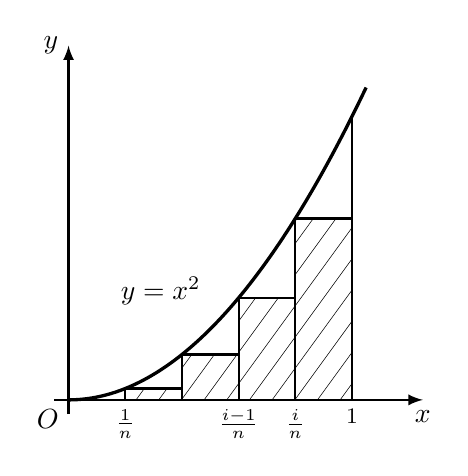
\begin{tikzpicture}[>=latex, scale=3.6]
  % 坐标轴
  \draw[->, thick] (-0.05, 0) -- (1.25, 0) node[below] {$x$};
  \draw[->, thick] (0, -0.05) -- (0, 1.25) node[left] {$y$};
  \node[below left] at (0, 0) {$O$};

  % 抛物线 y = x^2
  \draw[very thick, domain=0:1.05, smooth, samples=50] plot (\x, {\x*\x});
  \node[above left] at (0.5, 0.3) {$y=x^2$};

  % 阶梯小矩形 (示意以直代曲)
  % 矩形 i: [ (i-1)/n, i/n ], 高度 ((i-1)/n)^2
  \foreach \k/\h in {0.2/0.04, 0.4/0.16, 0.6/0.36, 0.8/0.64} {
    \draw[thick] (\k, 0) -- (\k, \h) -- (\k+0.2, \h) -- (\k+0.2, 0);
    \begin{scope}
      \clip (\k, 0) rectangle (\k+0.2, \h);
      \foreach \s in {-0.3, -0.22, ..., 1.2} {
        \draw[very thin] (\s, -0.3) -- (\s+0.8, 0.8);
      }
    \end{scope}
  }

  % x = 1 处的竖线到抛物线 (1,1)
  \draw[thick] (1, 0) -- (1, 1);

  % 轴上刻度与标注
  \node[below] at (0.2, 0) {\footnotesize $\frac{1}{n}$};
  \node[below] at (0.6, 0) {\footnotesize $\frac{i-1}{n}$};
  \node[below] at (0.8, 0) {\footnotesize $\frac{i}{n}$};
  \node[below] at (1.0, 0) {\footnotesize $1$};

  \draw (0.2, 0) -- (0.2, 0.02);
  \draw (0.4, 0) -- (0.4, 0.02);
  \draw (0.6, 0) -- (0.6, 0.02);
  \draw (0.8, 0) -- (0.8, 0.02);
  \draw (1.0, 0) -- (1.0, 0.02);
\end{tikzpicture}
\caption{}\label{fig:1.2.1}
\end{figure}

\begin{align*}
S &= \lim_{n\to+\infty}\left(\Delta S_{1}+\Delta S_{2}+\cdots+\Delta S_{n}\right) \\
&= \lim_{n\to+\infty}\frac{1}{n}\left[\left(\frac{1}{n}\right)^{2}+\left(\frac{2}{n}\right)^{2}+\cdots+\left(\frac{n-1}{n}\right)^{2}\right] \\
&= \lim_{n\to+\infty}\frac{1^{2}+2^{2}+\cdots+(n-1)^{2}}{n^{3}} = \lim_{n\to+\infty}\frac{(n-1)n(2n-1)}{6n^{3}} \\
&= \frac{1}{6}\lim_{n\to+\infty}\left(1-\frac{1}{n}\right)\left(2-\frac{1}{n}\right) = \frac{1}{3}.
\end{align*}
\end{solution}

\begin{example}\label{ex:1.2.5}
求下列极限：
\begin{enumerate}
  \item $\lim\limits_{n \to +\infty} (\sqrt{n+3} - \sqrt{n+1})$；
  \item $\lim\limits_{n \to +\infty} (\sqrt[3]{n+3} - \sqrt[3]{n+1})$；
  \item $\lim\limits_{n \to +\infty}\sqrt[n]{\lg n}$；
  \item $\lim\limits_{n\to+\infty}\sqrt[n]{a_1^n+a_2^n+\cdots+a_m^n}$（$a_i\geqslant0, i=1,2,\cdots,m$）；
  \item $\lim\limits_{n \to +\infty} [(n+1)^k - n^k]$（$0 < k < 1$）；
  \item $\lim\limits_{n \to +\infty} \left( \frac{1}{\sqrt{n^2 + 1}} + \cdots + \frac{1}{\sqrt{n^2 + n}} \right)$；
  \item $\lim\limits_{n \to +\infty} \frac{n^k}{a^n}$（$a > 1$）。
\end{enumerate}
\end{example}

\begin{solution}
(1) 因为
\[
0 < \sqrt{n+3}-\sqrt{n+1} = \frac{2}{\sqrt{n+3}+\sqrt{n+1}} < \frac{1}{\sqrt{n}} \to 0\quad (n\to+\infty),
\]
所以，由夹逼定理（或 $\varepsilon\text{-}N$ 法）知
\[
\lim_{n\to+\infty}(\sqrt{n+3}-\sqrt{n+1}) = 0.
\]

(2) 因为
\begin{align*}
0 &< \sqrt[3]{n+3}-\sqrt[3]{n+1} = \frac{2}{(\sqrt[3]{n+3})^2+\sqrt[3]{n+3}\sqrt[3]{n+1}+(\sqrt[3]{n+1})^2} \\
&< \frac{2}{3(\sqrt[3]{n})^2} = \frac{2}{3n^{\frac{2}{3}}} \to 0\quad (n\to+\infty),
\end{align*}
所以，由夹逼定理（或 $\varepsilon\text{-}N$ 法）知，
\[
\lim_{n\to+\infty}(\sqrt[3]{n+3}-\sqrt[3]{n+1}) = 0.
\]

(3) 因为
\[
10^{n} = (1+9)^{n} > 9n > n \iff 10 > n^{\frac{1}{n}} \iff 1 > \lg n^{\frac{1}{n}} = \frac{\lg n}{n} \iff \lg n < n,
\]
所以，
\[
\sqrt[n]{\lg 2} \leqslant \sqrt[n]{\lg n} < \sqrt[n]{n}.
\]
再由 $\lim\limits_{n\to+\infty}\sqrt[n]{\lg2} = 1 = \lim\limits_{n\to+\infty}\sqrt[n]{n}$ 及夹逼定理就得到
\[
\lim_{n\to+\infty}\sqrt[n]{\lg n} = 1.
\]
\textbf{注意}：虽然数列 $\{\sqrt[n]{a}\}$ 与数列 $\{\sqrt[n]{n}\}$ 的极限相同，但二者之间留有很大的空隙，这使得应用夹逼定理有极大的施展余地。

(4) 由下列不等式
\begin{align*}
\max\{a_{1},a_{2},\cdots,a_{m}\} &= \sqrt[n]{(\max\{a_{1},a_{2},\cdots,a_{m}\})^{n}} \leqslant \sqrt[n]{a_{1}^{n}+a_{2}^{n}+\cdots+a_{m}^{n}} \\
&\leqslant \sqrt[n]{n \cdot (\max\{a_{1},a_{2},\cdots,a_{m}\})^{n}} \\
&= \sqrt[n]{n}\max\{a_{1},a_{2},\cdots,a_{m}\} \to 1 \cdot \max\{a_{1},a_{2},\cdots,a_{m}\} \\
&= \max\{a_{1},a_{2},\cdots,a_{m}\}\quad (n\to+\infty)
\end{align*}
和夹逼定理知，
\[
\lim_{n\to+\infty}\sqrt[n]{a_{1}^{n}+a_{2}^{n}+\cdots+a_{m}^{n}} = \max\{a_{1},a_{2},\cdots,a_{m}\}.
\]

(5) 因为有不等式
\begin{align*}
0 < (n+1)^{k}-n^{k} &= n^{k}\left[\left(1+\frac{1}{n}\right)^{k}-1\right] < n^{k}\left[\left(1+\frac{1}{n}\right)-1\right] \\
&= \frac{1}{n^{1-k}} \to 0\quad (n\to+\infty),
\end{align*}
所以，由夹逼定理（或 $\varepsilon\text{-}N$ 法）得
\[
\lim_{n\to+\infty}[(n+1)^k-n^k] = 0.
\]

(6) 由不等式
\[
\frac{1}{1+\frac{1}{n}} < \frac{1}{\sqrt{1+\frac{1}{n}}} = \frac{n}{\sqrt{n^{2}+n}} \leqslant \frac{1}{\sqrt{n^{2}+1}}+\cdots+\frac{1}{\sqrt{n^{2}+n}} \leqslant \frac{n}{\sqrt{n^{2}+1}} < 1,
\]
$\lim\limits_{n\to+\infty}\frac{1}{1+\frac{1}{n}} = 1 = \lim\limits_{n\to+\infty}1$，以及夹逼定理立即可得
\[
\lim_{n\to+\infty}\left(\frac{1}{\sqrt{n^2+1}}+\cdots+\frac{1}{\sqrt{n^2+n}}\right) = 1.
\]

(7) 因 $a>1$，故 $\alpha = a-1 > 0$。从而
\[
0 < \frac{n^{k}}{a^{n}} = \frac{n^{k}}{(1+\alpha)^{n}} \leqslant \frac{n^{[|k|]+1}}{\mathrm{C}_{n}^{[|k|]+2}\alpha^{[|k|]+2}} \to 0\quad (n\to+\infty),
\]
再根据夹逼定理，就得 $\lim\limits_{n\to+\infty}\frac{n^k}{a^n} = 0$。
\end{solution}

\begin{example}\label{ex:1.2.6}
\begin{enumerate}
  \item 设 $a_{n} \geqslant 0$（$n \in \mathbb{N}$），$\lim\limits_{n \to +\infty} a_{n} = 0$，则 $\lim\limits_{n \to +\infty} \sqrt[n]{a_1 a_2 \cdots a_n} = 0$；
  \item 设 $a_n > 0$（$n \in \mathbb{N}$），$\lim\limits_{n \to +\infty} a_n = a > 0$，则 $\lim\limits_{n \to +\infty} \sqrt[n]{a_1 a_2 \cdots a_n} = a$。
\end{enumerate}
\end{example}

\begin{proof}
(1) 由 $0 \leqslant \sqrt[n]{a_1 a_2 \cdots a_n} \leqslant \frac{a_1 + a_2 + \cdots + a_n}{n} \to 0$（$n \to +\infty$），及夹逼定理，立即可得 $\lim\limits_{n \to +\infty} \sqrt[n]{a_1 a_2 \cdots a_n} = 0$。

(2) 当 $a>0, a_{n}>0$（$n\in\mathbb{N}$）时，有
\[
\frac{1}{\left(\frac{1}{a_{1}}+\frac{1}{a_{2}}+\cdots+\frac{1}{a_{n}}\right)/n} = \frac{n}{\frac{1}{a_{1}}+\frac{1}{a_{2}}+\cdots+\frac{1}{a_{n}}} \leqslant \sqrt[n]{a_{1}a_{2}\cdots a_{n}} \leqslant \frac{a_{1}+a_{2}+\cdots+a_{n}}{n},
\]
再由 $\lim\limits_{n\to+\infty}\frac{1}{\left(\frac{1}{a_1}+\frac{1}{a_2}+\cdots+\frac{1}{a_n}\right)/n} = \frac{1}{\frac{1}{a}} = a = \lim\limits_{n\to+\infty}\frac{a_1+a_2+\cdots+a_n}{n}$ 和夹逼定理，可得
\[
\lim_{n\to+\infty}\sqrt[n]{a_{1}a_{2}\cdots a_{n}} = a.
\]
\end{proof}

\begin{example}\label{ex:1.2.7}
设 $\lim\limits_{n\to+\infty}\sqrt[n]{|a_n|}=r>1$，则 $\lim\limits_{n\to+\infty}a_n=\infty$。
\end{example}

\begin{proof}
\textbf{证法 1} 取 $\varepsilon_{0}>0$，使得 $r-\varepsilon_{0} = 1+\alpha > 1$。因为 $\lim\limits_{n\to+\infty}\sqrt[n]{|a_{n}|} = r > 1$，故 $\exists N_{1}\in\mathbb{N}$，当 $n>N_{1}$ 时，有
\[
1+\alpha = r-\varepsilon_{0} < \sqrt[n]{|a_{n}|},\quad |a_{n}| > (1+\alpha)^{n} > n\alpha.
\]
$\forall A>0$，取 $N\in\mathbb{N}$，使得 $N > \max\left\{N_{1}, \frac{A}{\alpha}\right\}$，当 $n>N$ 时，有
\[
|a_{n}| > n\alpha > N\alpha \geqslant A.
\]
这就证明了 $\lim\limits_{n\to+\infty}a_n=\infty$。

\textbf{证法 2} 由上述，当 $n > N_{1}$ 时，有
\begin{align*}
1+\alpha &= r-\varepsilon_{0} < \sqrt[n]{|a_{n}|} < r+\varepsilon_{0} \\
&= (r-\varepsilon_{0})+2\varepsilon_{0} = 1+\alpha+2\varepsilon_{0},
\end{align*}
即 $(1+\alpha)^{n} < |a_{n}| < (1+\alpha+2\varepsilon_{0})^{n}$。所以，从 $\lim\limits_{n\to+\infty}(1+\alpha)^n = +\infty = \lim\limits_{n\to+\infty}(1+\alpha+2\varepsilon_0)^n$ 与夹逼定理可知，
\[
\lim_{n\to+\infty}|a_{n}|=+\infty \iff \lim_{n\to+\infty}a_{n}=\infty.
\]
\end{proof}

\begin{example}\label{ex:1.2.8}
设 $a_{n} \geqslant 0$（$n \in \mathbb{N}$），$\lim\limits_{n \to +\infty} \frac{a_{1} + 2a_{2} + \cdots + na_{n}}{\sqrt{n}} = a$，则
\[
\lim_{n\to+\infty}\sqrt{n} \cdot \sqrt[n]{a_{1}a_{2}\cdots a_{n}} = 0.
\]
\end{example}

\begin{proof}
\textbf{证法 1} 因为
\begin{align*}
0 &\leqslant \sqrt{n}\sqrt[n]{a_{1}a_{2}\cdots a_{n}} = \sqrt{n}\frac{\sqrt[n]{a_1 \cdot 2a_2 \cdots na_n}}{\sqrt[n]{n!}} \\
&\leqslant \frac{\sqrt{n}}{\sqrt[n]{n!}}\frac{a_{1}+2a_{2}+\cdots+na_{n}}{n} \\
&= \frac{1}{\sqrt[n]{n!}}\frac{a_{1}+2a_{2}+\cdots+na_{n}}{\sqrt{n}} \to 0 \cdot a = 0\quad (n\to+\infty),
\end{align*}
所以，根据夹逼定理，得到
\[
\lim_{n\to+\infty}\sqrt{n} \cdot \sqrt[n]{a_{1}a_{2}\cdots a_{n}} = 0.
\]

\textbf{证法 2} 由 $k(n-k+1)=(k-1)(n-k)+n \geqslant n$（$1 \leqslant k \leqslant n$）推得
\[
(n!)^{2} = (n\cdot 1)[(n-1)\cdot 2]\cdots(1\cdot n) \geqslant \underbrace{n \cdots n}_{n\text{ 个}} = n^{n}
\]
（或用数学归纳法证明）。于是，
\begin{align*}
0 &\leqslant \sqrt{n} \cdot \sqrt[n]{a_{1}a_{2}\cdots a_{n}} = \sqrt[n]{a_{1}a_{2}\cdots a_{n}n^{\frac{n}{2}}} \leqslant \sqrt[n]{a_{1}a_{2}\cdots a_{n}n!} \\
&= \sqrt[n]{a_{1}\cdot 2a_{2}\cdots na_{n}} \leqslant \frac{a_{1}+2a_{2}+\cdots+na_{n}}{n} \\
&= \frac{1}{\sqrt{n}}\frac{a_{1}+2a_{2}+\cdots+na_{n}}{\sqrt{n}} \to 0 \cdot a = 0\quad (n\to+\infty).
\end{align*}
根据夹逼定理知，$\lim\limits_{n\to+\infty}\sqrt{n}\cdot\sqrt[n]{a_1a_2\cdots a_n}=0$。
\end{proof}

\begin{exblock}{练习题 1.2}
\item 应用数列极限的基本性质求下列极限：
\begin{enumerate}
  \item $\lim\limits_{n\to+\infty}\frac{4n^2-n+5}{3n^2-2n-7}$；
  \item $\lim\limits_{n\to+\infty}\frac{3^n+(-2)^n}{3^{n+1}+(-2)^{n+1}}$；
  \item $\lim\limits_{n\to+\infty}\left(1-\frac{1}{n}\right)^{\frac{1}{n}}$；
  \item $\lim\limits_{n\to+\infty}(2\sin^{2}n+\cos^{2}n)^{\frac{1}{n}}$；
  \item $\lim\limits_{n \to +\infty} (\operatorname{arctan} n)^{\frac{1}{n}}$；
  \item $\lim\limits_{n \to +\infty} \frac{1+a+\cdots+a^{n-1}}{1+b+\cdots+b^{n-1}}$，$|a|<1, |b|<1$；
  \item $\lim\limits_{n \to +\infty} \left( \frac{1}{1 \cdot 2} + \frac{1}{2 \cdot 3} + \cdots + \frac{1}{n(n+1)} \right)$；
  \item $\lim\limits_{n \to +\infty} \left(1 - \frac{1}{2^2}\right) \left(1 - \frac{1}{3^2}\right) \cdots \left(1 - \frac{1}{n^2}\right)$；
  \item $\lim\limits_{n \to +\infty} \left( \frac{1}{2} + \frac{3}{2^2} + \cdots + \frac{2n-1}{2^n} \right)$；
  \item $\lim\limits_{n \to +\infty} \left(1 - \frac{1}{1+2}\right) \left(1 - \frac{1}{1+2+3}\right) \cdots \left(1 - \frac{1}{1+2+\cdots+n}\right)$；
  \item $\lim\limits_{n \to +\infty} \left[ \frac{1^2}{n^3} + \frac{2^2}{n^3} + \cdots + \frac{(2n-1)^2}{n^3} \right]$；
  \item $\lim\limits_{n \to +\infty} (1 + x)(1 + x^2)(1 + x^4) \cdots (1 + x^{2^{n-1}})$，其中 $|x| < 1$；
  \item $\lim\limits_{n \to +\infty} (\sqrt{n+2} - 2\sqrt{n+1} + \sqrt{n})$。
\end{enumerate}

\item 设 $a_{n} > 0, n \in \mathbb{N}$，$\lim\limits_{n \to +\infty} \frac{a_{n+1}}{a_n} = a$。应用例~\ref{ex:1.2.6} 证明：$\lim\limits_{n \to +\infty} \sqrt[n]{a_n} = a$。

\item 设 $\lim\limits_{n \to +\infty} a_n = a$。应用夹逼定理证明：$\lim\limits_{n \to +\infty} \frac{[na_n]}{n} = a$，其中 $[x]$ 表示不超过 $x$ 的最大整数。

\item 设 $a_{n} \neq 0$ 且 $\lim\limits_{n \to +\infty} \left| \frac{a_{n+1}}{a_n} \right| = r > 1$。证明：$\lim\limits_{n \to +\infty} a_{n} = \infty$。

\item 
\begin{enumerate}
  \item 应用数学归纳法或 $\frac{2k-1}{2k} < \frac{2k}{2k+1}$ 证明不等式：
  \[
  \frac{1}{2} \cdot \frac{3}{4} \cdot \cdots \cdot \frac{2n-1}{2n} < \frac{1}{\sqrt{2n+1}};
\]
  \item 证明：$\lim\limits_{n \to +\infty} \left( \frac{1}{2} \cdot \frac{3}{4} \cdot \cdots \cdot \frac{2n-1}{2n} \right) = 0$。
\end{enumerate}

\item 设 $a_n > 0$（$n \in \mathbb{N}$）且 $\lim\limits_{n \to +\infty} a_n = a > 0$。应用夹逼定理证明：$\lim\limits_{n \to +\infty} \sqrt[n]{a_n} = 1$。

\item 证明：$\lim\limits_{n \to +\infty} \frac{\sum\limits_{k=1}^{n} k!}{n!} = 1$。（提示：$1 + \frac{1}{n} \leqslant \frac{\sum\limits_{k=1}^{n} k!}{n!} \leqslant 1 + \frac{2}{n}$）。

\item 设 $\lim\limits_{n\to+\infty}a_n=a$，$\lim\limits_{n\to+\infty}b_n=b$。记
\[
S_{n}=\max\{a_{n},b_{n}\},\quad T_{n}=\min\{a_{n},b_{n}\},\quad n=1,2,\cdots.
\]
应用 $\varepsilon\text{-}N$ 法（分 $a<b, a>b, a=b$）或 $\max\{a_n, b_n\} = \frac{1}{2}(a_n + b_n + |a_n - b_n|)$ 与 $\min\{a_{n},b_{n}\}=\frac{1}{2}(a_{n}+b_{n}-|a_{n}-b_{n}|)$，证明：
\begin{enumerate}
  \item $\lim\limits_{n \to +\infty} S_n = \max\{a, b\}$；
  \item $\lim\limits_{n \to +\infty} T_n = \min\{a, b\}$。
\end{enumerate}

\item 应用例 1.1.7 与例 1.1.15 证明：
\[
\lim_{n\to+\infty}\frac{1+\sqrt{2}+\sqrt[3]{3}+\cdots+\sqrt[n]{n}}{n}=1.
\]

\item 证明：$\lim\limits_{n\to+\infty}\left(\sin\frac{\ln2}{2}+\sin\frac{\ln3}{3}+\cdots+\sin\frac{\ln n}{n}\right)^{\frac{1}{n}}=1$。

\item 证明：$\lim\limits_{n \to +\infty} \sum\limits_{k=n^{2}}^{(n+1)^{2}} \frac{1}{\sqrt{k}} = 2$。
\end{exblock}

\begin{exblock}{思考题 1.2}
\item 用 $p(n)$ 表示能整除 $n$ 的素数的个数。证明：$\lim\limits_{n\to+\infty}\frac{p(n)}{n}=0$。
\item 设 $x_{n} = \sum\limits_{k=1}^{n} \left( \sqrt{1 + \frac{k}{n^{2}}} - 1 \right)$。证明：$\lim\limits_{n \to +\infty} x_{n} = \frac{1}{4}$。
\end{exblock}

\section{实数理论、实数连续性命题}\label{sec:1.3}

前面已讲过，实数是数学分析研究对象的根。为了进一步讨论数列极限的重要性，需要引进实数连续性命题，而实数连续性命题有七个，它们是彼此等价的。证明等价的方法是极其重要的，以后经常要引用。要想学好数学分析，一定要牢牢掌握这些内容和方法，以便今后灵活应用实数连续性的等价命题。

\begin{definition}\label{def:1.3.1}
如果数列 $\{a_{n}\}$ 满足：对任何自然数 $m, n$，$m < n$，有 $a_m \leqslant a_n$（或 $a_m \geqslant a_n$），则称数列 $\{a_n\}$ 为\textbf{单调增}（或\textbf{减}）\textbf{数列}，也称为\textbf{递增}（或\textbf{减}）\textbf{数列}。

如果数列 $\{a_{n}\}$ 满足：对任何自然数 $m, n$，$m < n$，有 $a_m < a_n$（或 $a_m > a_n$），则称数列 $\{a_n\}$ 为\textbf{严格增}（或\textbf{减}）\textbf{数列}，也称为\textbf{严格递增}（或\textbf{减}）\textbf{数列}。

单调增与单调减数列统称为\textbf{单调数列}；严格增与严格减数列统称为\textbf{严格单调数列}。
\end{definition}

\begin{definition}\label{def:1.3.2}
设 $A$ 为实数集 $\mathbb{R}$ 的子集（即 $A \subset \mathbb{R}$）。如果存在实数 $M$，使对任何 $x \in A$，有 $x \leqslant M$（或 $x \geqslant M$），则称 $M$ 为数集 $A$ 的一个\textbf{上}（或\textbf{下}）\textbf{界}。

如果数集 $A$ 既有上界又有下界，则称 $A$ 为\textbf{有界集}。

显然，$A$ 有界的充分必要条件是存在实数 $M$，使得对任意 $x \in A$，有 $|x| \leqslant M$。

由下面的实数连续性命题（一），有上（下）界的非空数集必有最小（大）上（下）界，因此可以定义上（下）确界。
\end{definition}

\begin{definition}\label{def:1.3.3}
如果非空数集 $A$ 有上（下）界，则称其最小（大）上（下）界为 $A$ 的\textbf{上}（或\textbf{下}）\textbf{确界}，记为 $\sup A$（$\inf A$）。

如果非空数集 $A$ 无上（下）界，则定义 $A$ 的上（下）确界为 $+\infty$（$-\infty$），即 $\sup A = +\infty$（$\inf A = -\infty$）。
\end{definition}

对自然数集 $\mathbb{N}$，有理数集 $\mathbb{Q}$，实数集 $\mathbb{R}$，容易看出：
\[
\inf \mathbb{N} = 1,\quad \sup \mathbb{N} = +\infty,\quad \inf \mathbb{Q} = -\infty,\quad \sup \mathbb{Q} = +\infty,\quad \inf \mathbb{R} = -\infty,\quad \sup \mathbb{R} = +\infty.
\]

\begin{example}\label{ex:1.3.1}
\begin{align*}
&\inf[0,1) = 0,\quad \sup[0,1) = 1; \\
&\inf(0,1) = 0,\quad \sup(0,1) = 1; \\
&\inf\{\sin x \mid x \in \mathbb{R}\} = -1,\quad \sup\{\sin x \mid x \in \mathbb{R}\} = 1; \\
&\inf\{\operatorname{arctan} x \mid x \in \mathbb{R}\} = -\frac{\pi}{2},\quad \sup\{\operatorname{arctan} x \mid x \in \mathbb{R}\} = \frac{\pi}{2}; \\
&\inf\left\{\frac{1}{n}\;\middle|\; n \in \mathbb{N}\right\} = 0,\quad \sup\left\{\frac{1}{n}\;\middle|\; n \in \mathbb{N}\right\} = 1; \\
&\inf\{a_1, a_2, \cdots, a_m\} = \min\{a_1, a_2, \cdots, a_m\}; \\
&\sup\{a_1, a_2, \cdots, a_m\} = \max\{a_1, a_2, \cdots, a_m\}.
\end{align*}
\end{example}

\begin{definition}\label{def:1.3.4}
设 $U \subset \mathbb{R}$，如果对任意的 $x \in U$，存在 $\delta(x) > 0$，使得集合
\[
B(x;\delta(x)) = \{y \in \mathbb{R} \mid \rho(y, x) < \delta(x)\} = (x - \delta(x), x + \delta(x)) \subset U,
\]
则称 $U$ 为 $\mathbb{R}$ 中的\textbf{开集}，含 $x \in U$ 的开集称为 $x$ 的\textbf{开邻域}。显然，任何（有限或无限）开区间都为 $\mathbb{R}$ 中的开集。

如果 $F$（$\subset \mathbb{R}$）的补（余）集 $F^c = \mathbb{R} \setminus F$ 为 $\mathbb{R}$ 中的开集，则称 $F$ 为 $\mathbb{R}$ 中的\textbf{闭集}。例如，$[a,b], (-\infty, a], [a, +\infty)$ 都为闭集。
\end{definition}

\begin{definition}\label{def:1.3.5}
设 $A \subset \mathbb{R}$，$x_0 \in \mathbb{R}$（未必 $x_0 \in A$）。如果对 $x_0$ 的任何开邻域 $U$，均含有 $A$ 中异于 $x_0$ 的点，即
\[
U \cap (A \setminus \{x_0\}) \neq \varnothing,
\]
则称 $x_0$ 为 $A$ 的一个\textbf{聚点}。$A$ 的聚点的全体记为 $A'$。$\overline{A} = A \cup A'$ 称为 $A$ 的\textbf{闭包}。

易证，$x_0$ 为 $A$ 的聚点 $\iff x_0$ 的任何开邻域 $U$，均含 $A$ 中无限个点。

显然，$\mathbb{Q}' = \mathbb{R}$，$(\mathbb{R} \setminus \mathbb{Q})' = \mathbb{R}$。
\end{definition}

\begin{definition}\label{def:1.3.6}
设 $\{a_n\}$ 为 $\mathbb{R}$ 中的一个数列，如果 $\forall \varepsilon > 0$，$\exists N \in \mathbb{N}$，当 $m, n > N$ 时，有
\[
\rho(a_n, a_m) = |a_n - a_m| < \varepsilon,
\]
则称 $\{a_n\}$ 为 \textbf{Cauchy 数列}或\textbf{基本数列}。它等价于 $\forall \varepsilon > 0$，$\exists N \in \mathbb{N}$，当 $n > N$ 时，$\forall p \in \mathbb{N}$，有
\[
\rho(a_n, a_{n+p}) = |a_n - a_{n+p}| < \varepsilon.
\]
\end{definition}

下面将给出七个彼此等价的实数连续性命题，它渗透到微分学与积分学，即数学分析的每一个角落，是数学分析的极其重要的基础。读者必须清楚它的理论知识与方法，更重要的是能熟练地应用它。

\begin{proposition}[实数连续性命题（一），确界存在定理]\label{prop:cont:1}
有上（下）界的非空数集必有属于 $\mathbb{R}$ 的最小（大）上（下）界，即有有限的上（下）确界。
\end{proposition}

\begin{proposition}[实数连续性命题（二），单调有界原理]\label{prop:cont:2}
单调增（减）有上（下）界的数列必收敛。
\end{proposition}

\begin{proposition}[实数连续性命题（三），闭区间套原理，Cantor]\label{prop:cont:3}
设递降闭区间序列
\[
[a_1, b_1] \supset [a_2, b_2] \supset \cdots \supset [a_n, b_n] \supset \cdots,
\]
其长度 $b_n - a_n \to 0$（$n \to +\infty$），则 $\exists_1 x_0 \in \bigcap\limits_{n=1}^\infty [a_n, b_n]$，即 $x_0 \in [a_n, b_n]$，$\forall n \in \mathbb{N}$（$\exists_1$ 表示存在惟一）。
\end{proposition}

\begin{proposition}[实数连续性命题（四），有限覆盖定理，Heine-Borel]\label{prop:cont:4}
$[a,b]$ 的任何开覆盖 $\mathcal{I}$（$\mathcal{I}$ 中的元素均为开集，且对 $\forall x \in [a,b]$，必有开集 $U \in \mathcal{I}$，使得 $x \in U$，或 $[a,b] \subset \bigcup\limits_{U \in \mathcal{I}} U$）必有有限子覆盖（即存在 $\{U_1, U_2, \cdots, U_m\} \subset \mathcal{I}$ 覆盖 $[a,b]$，即 $[a,b] \subset \bigcup\limits_{k=1}^m U_k$）。
\end{proposition}

\begin{proposition}[实数连续性命题（五），Weierstrass 聚点定理]\label{prop:cont:5}
有界无限数集 $A$ 必有聚点 $x_0 \in \mathbb{R}$。
\end{proposition}

\begin{proposition}[实数连续性命题（六），Bolzano-Weierstrass 致密性定理]\label{prop:cont:6}
有界数列必有收敛子列。
\end{proposition}

\begin{proposition}[实数连续性命题（七），Cauchy 完备性原理]\label{prop:cont:7}
Cauchy 数列（基本数列）必收敛（此时，$(\mathbb{R}, \rho)$ 称为完备度量空间）。
\end{proposition}

\begin{theorem}[实数连续性等价命题]\label{thm:1.3.1}
七个实数连续性命题是彼此等价的。
\end{theorem}

\begin{proof}
我们按（一）$\implies$（二）$\implies$（三）$\implies$（四）$\implies$（五）$\implies$（六）$\implies$（七）$\implies$（一）进行循环证明。

\textbf{（一）$\implies$（二）} 设数列 $\{a_n\}$ 单调增有上界，根据实数连续性命题（一），它有有限的上确界 $\alpha = \sup\limits_{n\in\mathbb{N}} a_n < +\infty$。

$\forall \varepsilon > 0$，根据 $\alpha$ 为上确界的定义，$\alpha - \varepsilon$（$< \alpha$）不是数列 $\{a_n\}$ 的上界，因此存在 $n_\varepsilon \in \mathbb{N}$，使得 $a_{n_\varepsilon} > \alpha - \varepsilon$。又因 $\{a_n\}$ 单调增，故当 $n > n_\varepsilon$ 时，有
\[
\alpha - \varepsilon < a_{n_\varepsilon} \leqslant a_n \leqslant \alpha < \alpha + \varepsilon.
\]
所以，
\[
\lim_{n\to+\infty} a_n = \alpha = \sup_{n\in\mathbb{N}} a_n.
\]
对单调减有下界的情形类似可证 $\lim\limits_{n\to+\infty} a_n = \inf\limits_{n\in\mathbb{N}} a_n$，或者应用上述结论于 $\{-a_n\}$。

\textbf{（二）$\implies$（三）} 由题设得到两个单调有界数列
\[
b_1 \geqslant b_2 \geqslant \cdots \geqslant b_n \geqslant \cdots \geqslant a_1,
\]
\[
a_1 \leqslant a_2 \leqslant \cdots \leqslant a_n \leqslant \cdots \leqslant b_1.
\]
根据实数连续性命题（二）知，数列 $\{a_n\}$ 与 $\{b_n\}$ 均收敛。又由题设，有
\[
\lim_{n\to+\infty} b_n - \lim_{n\to+\infty} a_n = \lim_{n\to+\infty} (b_n - a_n) = 0,
\]
即数列 $\{a_n\}$ 与 $\{b_n\}$ 收敛于同一数，记为 $x_0$。再由实数连续性命题（二），
\[
\sup_{n\in\mathbb{N}} a_n = \lim_{n\to+\infty} a_n = x_0 = \lim_{n\to+\infty} b_n = \inf_{n\in\mathbb{N}} b_n.
\]
所以，
\[
a_n \leqslant \sup_{m\in\mathbb{N}} a_m = x_0 = \inf_{m\in\mathbb{N}} b_m \leqslant b_n,\quad \forall n \in \mathbb{N},
\]
即
\[
x_0 \in \bigcap_{n=1}^\infty [a_n, b_n].
\]
如果还有 $x_1 \in \bigcap\limits_{n=1}^\infty [a_n, b_n]$，则
\[
|x_1 - x_0| \leqslant b_n - a_n,\quad \forall n \in \mathbb{N}.
\]
从而
\[
0 \leqslant |x_1 - x_0| \leqslant \lim_{n\to+\infty} (b_n - a_n) = 0 \implies x_1 - x_0 = 0 \implies x_1 = x_0.
\]
这就证明了 $\exists_1 x_0 \in \bigcap\limits_{n=1}^\infty [a_n, b_n]$。

\textbf{（三）$\implies$（四）} （反证）反设区间 $[a,b]$ 不能被 $\mathcal{I}$ 中有限个开集所覆盖。将 $[a,b]$ 等分为两个闭区间 $\left[a, \frac{a+b}{2}\right]$ 与 $\left[\frac{a+b}{2}, b\right]$，则此两个区间中必有一个不能被 $\mathcal{I}$ 中有限个开集所覆盖，记此区间为 $[a_1, b_1]$。再将 $[a_1, b_1]$ 等分为二，二者中又必有一个不能被 $\mathcal{I}$ 中有限个开集所覆盖，记此区间为 $[a_2, b_2]$。如此下去，得一递降闭区间序列：
\[
[a_1, b_1] \supset [a_2, b_2] \supset \cdots \supset [a_n, b_n] \supset \cdots,
\]
其中每一个都不能被 $\mathcal{I}$ 中有限个开集所覆盖，且长度
\[
b_n - a_n = \frac{b-a}{2^n} \to 0\quad (n \to +\infty).
\]
因此，由连续性命题（三）（闭区间套原理），$\exists_1 x_0 \in \bigcap\limits_{n=1}^\infty [a_n, b_n]$。由于 $\mathcal{I}$ 覆盖 $[a,b]$，故必存在 $U_0 \in \mathcal{I}$，使得 $x_0 \in U_0$。但 $U_0$ 为开集，显然，$\exists N \in \mathbb{N}$，当 $n > N$ 时，有
\[
x_0 \in [a_n, b_n] \subset U_0.
\]
于是，区间 $[a_n, b_n]$ 被 $\mathcal{I}$ 中的一个（当然是有限个）开集所覆盖。这与上面构造 $[a_n, b_n]$ 不被 $\mathcal{I}$ 中有限个开集所覆盖相矛盾。

\textbf{（四）$\implies$（五）} 设 $A$ 为有界无限集，即 $A \subset [a,b]$。（反证）反设 $A$ 无聚点，则 $\forall x \in [a,b]$，$x$ 不为 $A$ 的聚点，故必有开区间（当然它为开集）$I_x \ni x$，且 $I_x$ 中最多只含 $A$ 的一个点 $x$。显然，开区间族
\[
\mathcal{I} = \{I_x \mid x \in [a,b]\}
\]
覆盖了 $[a,b]$。根据连续性命题（四）（紧致性）知，$\exists \{I_{x_1}, I_{x_2}, \cdots, I_{x_m}\} \subset \mathcal{I}$，使得 $[a,b] \subset \bigcup\limits_{k=1}^m I_{x_k}$。

因此，$\bigcup\limits_{k=1}^m I_{x_k}$ 也覆盖住 $A$。但是，每个 $I_{x_k}$ 至多含 $A$ 的一个点。由此推得 $\bigcup\limits_{k=1}^m I_{x_k}$ 至多只含 $A$ 的有限个点，而不能覆盖住整个无限集 $A$，矛盾。

\textbf{（五）$\implies$（六）} 设数列 $\{a_n\}$ 有界，即 $a \leqslant a_n \leqslant b$，$\forall n \in \mathbb{N}$。如果 $\{a_n \mid n \in \mathbb{N}\}$ 为有限集，则数列 $\{a_n\}$ 必有无限项相同，这些项依下标从小到大排列得到 $\{a_n\}$ 的一个收敛子列；如果 $A = \{a_n \mid n \in \mathbb{N}\}$ 为无限集，根据连续性命题（五）知，这个无限集 $A$ 必有一个聚点 $x_0$。由聚点定义，$(x_0 - 1, x_0 + 1)$ 中必有 $A$ 中一点 $a_{n_1} \neq x_0$。令
\[
\delta_1 = \min\left\{\frac{1}{2}, \rho(a_i, x_0) > 0 \;\middle|\; i = 1, 2, \cdots, n_1\right\} > 0,
\]
再由聚点定义知，$(x_0 - \delta_1, x_0 + \delta_1)$ 中必有 $A$ 中一点 $a_{n_2} \neq x_0$。显然，$0 < \delta_1 < \frac{1}{2}$，$n_1 < n_2$。依此类推，令
\[
\delta_k = \min\left\{\frac{1}{k+1}, \rho(a_i, x_0) > 0 \;\middle|\; i = 1, 2, \cdots, n_k\right\} > 0.
\]
由聚点定义知，$(x_0 - \delta_k, x_0 + \delta_k)$ 中必有 $A$ 中一点 $a_{n_{k+1}} \neq x_0$。显然 $0 < \delta_k < \frac{1}{k+1}$，$n_k < n_{k+1}$。容易看出 $\{a_{n_k}\}$ 为收敛于 $x_0$ 的数列 $\{a_n\}$ 的子列。

\textbf{（六）$\implies$（七）} 设 $\{a_n\}$ 为 Cauchy 数列（基本数列）。先证 $\{a_n\}$ 有界。取 $\varepsilon = 1$，故 $\exists n_1 \in \mathbb{N}$，使得当 $m, n > n_1$ 时，有
\[
|a_m - a_n| < \varepsilon = 1.
\]
于是，当 $n > n_1$ 时，
\[
|a_n| \leqslant |a_n - a_{n_1+1}| + |a_{n_1+1}| < 1 + |a_{n_1+1}|.
\]
由此得到
\[
|a_n| \leqslant \max\{|a_1|, \cdots, |a_{n_1}|, 1 + |a_{n_1+1}|\} = M < +\infty,
\]
即数列 $\{a_n\}$ 是有界的。

根据实数连续性命题（六）（序列紧性）知，有界数列 $\{a_n\}$ 有收敛子列 $\{a_{n_k}\}$。设 $a = \lim\limits_{k\to+\infty} a_{n_k}$。下面证 $\{a_n\}$ 也收敛于 $a$。

事实上，$\forall \varepsilon > 0$，$\exists K_\varepsilon \in \mathbb{N}$，当 $k > K_\varepsilon$ 时，有 $|a_{n_k} - a| < \frac{\varepsilon}{2}$。又因 $\{a_n\}$ 为 Cauchy 数列（基本数列），所以又有 $n_\varepsilon \in \mathbb{N}$，当 $m, n > n_\varepsilon$ 时，
\[
|a_m - a_n| < \frac{\varepsilon}{2}.
\]
再取 $k \in \mathbb{N}$，使得 $k > \max\{K_\varepsilon, n_\varepsilon\}$，则 $n_k \geqslant k > \max\{K_\varepsilon, n_\varepsilon\}$。当 $n > n_\varepsilon$ 时，
\[
|a_n - a| \leqslant |a_n - a_{n_k}| + |a_{n_k} - a| < \frac{\varepsilon}{2} + \frac{\varepsilon}{2} = \varepsilon,
\]
从而，$\{a_n\}$ 收敛于 $a$。

\textbf{（七）$\implies$（一）} 设非空数集 $A$ 有上界 $M$（有下界的情形类似证明；或考虑数集 $-A = \{-x \mid x \in A\}$）。

若 $M \in A$，则显然 $M = \sup A$。

若 $M \notin A$，在 $A$ 中任取一个数 $m$，则闭区间 $[m, M]$ 有 $A$ 中之数。将 $[m, M]$ 等分为二：$\left[m, \frac{m+M}{2}\right]$ 与 $\left[\frac{m+M}{2}, M\right]$。如果 $\left[\frac{m+M}{2}, M\right]$ 中有 $A$ 中之数，取 $a_1 = \frac{m+M}{2}, b_1 = M$；反之，取 $a_1 = m, b_1 = \frac{m+M}{2}$。于是，$b_1$ 为 $A$ 的上界，$[a_1, b_1]$ 有 $A$ 中之数。将 $[a_1, b_1]$ 等分为二：$\left[a_1, \frac{a_1+b_1}{2}\right]$ 与 $\left[\frac{a_1+b_1}{2}, b_1\right]$。如果 $\left[\frac{a_1+b_1}{2}, b_1\right]$ 中有 $A$ 中之数，取 $a_2 = \frac{a_1+b_1}{2}, b_2 = b_1$；反之，取 $a_2 = a_1, b_2 = \frac{a_1+b_1}{2}$。于是，$b_2$ 为 $A$ 的上界，$[a_2, b_2]$ 有 $A$ 中之数。如此下去，得到两个数列 $\{a_n\}$ 与 $\{b_n\}$，它们满足：
\begin{enumerate}
  \item $b_n$（$n \in \mathbb{N}$）都为 $A$ 的上界；
  \item $[a_n, b_n]$（$n \in \mathbb{N}$）都有 $A$ 中之数；
  \item $b_n - a_n = \dfrac{M-m}{2^n}$（$n \in \mathbb{N}$）；
  \item $|a_n - a_{n+1}| \leqslant \dfrac{M-m}{2^{n+1}},\quad |b_n - b_{n+1}| \leqslant \dfrac{M-m}{2^{n+1}}$（$n \in \mathbb{N}$）。
\end{enumerate}

易见，$\{a_n\}$ 与 $\{b_n\}$ 都为 Cauchy 数列（基本数列）。事实上，$\forall \varepsilon > 0$，取 $N \in \mathbb{N}$，使得 $N > \log_2 \frac{M-m}{\varepsilon}$，当 $n > N$ 时，$\forall p \in \mathbb{N}$，有
\begin{align*}
|a_n - a_{n+p}| &\leqslant |a_n - a_{n+1}| + |a_{n+1} - a_{n+2}| + \cdots + |a_{n+p-1} - a_{n+p}| \\
&\leqslant \frac{M-m}{2^{n+1}}\left(1 + \frac{1}{2} + \cdots + \frac{1}{2^{p-1}}\right) \\
&= \frac{M-m}{2^{n+1}}\frac{1-\frac{1}{2^p}}{1-\frac{1}{2}} < \frac{M-m}{2^n} < \frac{M-m}{2^N} < \varepsilon,
\end{align*}
故 $\{a_n\}$ 为 Cauchy 数列。类似可证 $\{b_n\}$ 也为 Cauchy 数列。

由实数连续性命题（七），已知 $\mathbb{R}$ 是完备的，因此 Cauchy 数列 $\{a_n\}$ 与 $\{b_n\}$ 均收敛。于是，由 (3)，$\{a_n\}$ 与 $\{b_n\}$ 收敛于同一数 $a$。又由 (1) 可知，$a$ 为 $A$ 的上界，所以区间 $(a, b_n]$（$n \in \mathbb{N}$）皆无 $A$ 中之数。根据 (2)，$[a_n, a]$（$n \in \mathbb{N}$）都有 $A$ 中之数，而 $a_n \to a$（$n \to +\infty$），故 $a$ 为 $A$ 的上确界（$\forall \varepsilon > 0$，$\exists a_n$，使得 $a - \varepsilon < a_n \leqslant a$，从而 $a - \varepsilon$ 不为 $A$ 的上界）。
\end{proof}

\begin{theorem}\label{thm:1.3.2}
设数列 $\{a_n\}$ 单调增（减）无上（下）界，则
\[
\lim_{n\to+\infty} a_n = +\infty\quad (-\infty).
\]
\end{theorem}

\begin{proof}
设 $\{a_n\}$ 单调增无上界，$\forall A > 0$，它不是 $\{a_n\}$ 的上界，故 $\exists N \in \mathbb{N}$，使得 $a_N > A$。当 $n \geqslant N$ 时，由 $\{a_n\}$ 单调增，可得
\[
a_n \geqslant a_N > A,
\]
这就证明了 $\lim\limits_{n\to+\infty} a_n = +\infty$。

类似可证，当 $\{a_n\}$ 单调减无下界时 $\lim\limits_{n\to+\infty} a_n = -\infty$。或应用上述结果于 $\{-a_n\}$，并由定理~\ref{thm:1.2.7}(6) 推得。
\end{proof}

\begin{corollary}\label{cor:1.3.1}
单调数列 $\{a_n\}$ 必有极限。
\end{corollary}

\begin{proof}
由定理~\ref{thm:1.3.1}（二）及定理~\ref{thm:1.3.2} 知，当 $\{a_n\}$ 为单调增时，
\[
\lim_{n\to+\infty} a_n = \sup_{n\in\mathbb{N}} a_n = \begin{cases}
\text{收敛于数 }\sup\limits_{n\in\mathbb{N}} a_n, & \text{当 }\{a_n\}\text{ 有上界时}, \\
\text{发散于 }+\infty, & \text{当 }\{a_n\}\text{ 无上界时};
\end{cases}
\]
当 $\{a_n\}$ 为单调减时，
\[
\lim_{n\to+\infty} a_n = \inf_{n\in\mathbb{N}} a_n = \begin{cases}
\text{收敛于数 }\inf\limits_{n\in\mathbb{N}} a_n, & \text{当 }\{a_n\}\text{ 有下界时}, \\
\text{发散于 }-\infty, & \text{当 }\{a_n\}\text{ 无下界时}.
\end{cases}
\]
\end{proof}

\begin{corollary}\label{cor:1.3.2}
单调数列收敛 $\iff$ 单调数列有一个收敛子列。
\end{corollary}

\begin{proof}
($\Rightarrow$) 设单调数列 $\{a_n\}$ 收敛，显然 $\{a_n\}$ 为一个特殊的子列 $\{a_{n_k}\}$（$n_k = k$）。因此，$\{a_n\}$ 本身为 $\{a_n\}$ 的一个收敛子列。

($\Leftarrow$) 不妨设数列 $\{a_n\}$ 是单调增的，它有一子列 $\{a_{n_k}\}$ 收敛。记 $\lim\limits_{k\to+\infty} a_{n_k} = a$。$\forall \varepsilon > 0$，$\exists K \in \mathbb{N}$，当 $k > K$ 时，
\[
a - \varepsilon < a_{n_k} \leqslant a < a + \varepsilon.
\]
令 $N = n_{K+1}$，则对任意的 $n > N$ 时，必有 $K' \in \mathbb{N}$，使得 $n_{K'} > n$，则
\[
a - \varepsilon < a_{n_{K+1}} \leqslant a_n \leqslant a_{n_{K'}} \leqslant a < a + \varepsilon,
\]
\[
\lim_{n\to+\infty} a_n = a.
\]
这就证明了数列 $\{a_n\}$ 收敛于 $a$。
\end{proof}

\begin{theorem}[数列的 Cauchy 收敛准则或收敛原理]\label{thm:1.3.3}
数列 $\{a_n\}$ 收敛 $\iff \{a_n\}$ 为 Cauchy 数列（基本数列）。
\end{theorem}

\begin{proof}
($\Rightarrow$) 设 $\{a_n\}$ 收敛，记 $\lim\limits_{n\to+\infty} a_n = a$，则 $\forall \varepsilon > 0$，$\exists N \in \mathbb{N}$，当 $n, m > N$ 时，有
\[
|a_n - a| < \frac{\varepsilon}{2},\quad |a_m - a| < \frac{\varepsilon}{2},
\]
因而，
\[
|a_n - a_m| \leqslant |a_n - a| + |a - a_m| < \frac{\varepsilon}{2} + \frac{\varepsilon}{2} = \varepsilon.
\]
这就证明了 $\{a_n\}$ 为 Cauchy 数列（基本数列）。

($\Leftarrow$) 由定理~\ref{thm:1.3.1}（六）$\implies$（七）。
\end{proof}

为揭示有理数与实数之间的本质差别，我们引入至多可数集与不可数集的概念。

\begin{definition}\label{def:1.3.7}
与自然数集 $\mathbb{N}$ 一一对应的集合称为\textbf{可数集}。有限集与可数集统称为\textbf{至多可数集}。不是至多可数集的集合称为\textbf{不可数集}。
\end{definition}

\begin{lemma}\label{lem:1.3.1}
\begin{enumerate}
  \item 至多可数集的子集仍为至多可数集；
  \item 有限个至多可数集的并仍为至多可数集；
  \item 可数个至多可数集的并仍为至多可数集；
  \item 设 $A_1, A_2, \cdots, A_n$ 都为至多可数集，则笛卡尔积集合
  \[
  A_1 \times A_2 \times \cdots \times A_n = \{(a_1, a_2, \cdots, a_n) \mid a_i \in A_i, i = 1, 2, \cdots, n\}
\]
  为至多可数集。
\end{enumerate}
\end{lemma}

\begin{proof}
(1) 设 $X$ 为至多可数集。记 $X = \{x_1, \cdots, x_n, \cdots\}$，则它的子集可记为 $\{x_{n_k} \mid n_1 < n_2 < \cdots\}$，显然，它仍为至多可数集。

(2) 设有限个可数集为
\begin{align*}
A_1 &= \{a_{11}, a_{12}, a_{13}, \cdots\}, \\
A_2 &= \{a_{21}, a_{22}, a_{23}, \cdots\}, \\
A_3 &= \{a_{31}, a_{32}, a_{33}, \cdots\}, \\
&\ \ \vdots \\
A_n &= \{a_{n1}, a_{n2}, a_{n3}, \cdots\},
\end{align*}
则 $\bigcup\limits_{i=1}^n A_i = \{a_{11}, a_{21}, \cdots, a_{n1}, a_{12}, a_{22}, \cdots, a_{n2}, \cdots\}$，如有重复者只排第 1 个，由此知 $\bigcup\limits_{i=1}^n A_i$ 仍为至多可数集。

或者按斜线排列为 $\bigcup\limits_{i=1}^n A_i = \{a_{11}, a_{21}, a_{12}, a_{31}, a_{22}, a_{13}, \cdots\}$，如有重复者只排第 1 个，由此知 $\bigcup\limits_{i=1}^n A_i$ 仍为至多可数集。

(3) 仿照 (2) 中第二种证法。

(4) 设
\begin{align*}
A_1 &= \{a_1^1, a_1^2, a_1^3, \cdots\}, \\
A_2 &= \{a_2^1, a_2^2, a_2^3, \cdots\}, \\
A_3 &= \{a_3^1, a_3^2, a_3^3, \cdots\}, \\
&\ \ \vdots \\
A_n &= \{a_n^1, a_n^2, a_n^3, \cdots\}.
\end{align*}
则 $A_1 \times A_2 \times \cdots \times A_n$ 按 $(a_1^{i_1}, a_2^{i_2}, \cdots, a_n^{i_n})$ 中 $i_1 + i_2 + \cdots + i_n$ 从小到大排列，故积集合 $A_1 \times A_2 \times \cdots \times A_n$ 为至多可数集。
\end{proof}

\begin{lemma}\label{lem:1.3.2}
有理数集 $\mathbb{Q}$ 为至多可数集。
\end{lemma}

\begin{proof}
将正有理数集按如下对角线箭头方向排列：
\[
\begin{array}
{ccccc}
\dfrac{1}{1} & \dfrac{2}{1} & \dfrac{3}{1} & \dfrac{4}{1} & \cdots \\[2mm]
\dfrac{1}{2} & \dfrac{2}{2} & \dfrac{3}{2} & \dfrac{4}{2} & \cdots \\[2mm]
\dfrac{1}{3} & \dfrac{2}{3} & \dfrac{3}{3} & \dfrac{4}{3} & \cdots \\[2mm]
\dfrac{1}{4} & \dfrac{2}{4} & \dfrac{3}{4} & \dfrac{4}{4} & \cdots \\
\vdots & \vdots & \vdots & \vdots & \ddots
\end{array}
\]
列为
\[
\mathbb{Q} = \left\{0, \frac{1}{1}, -\frac{1}{1}, \frac{1}{2}, -\frac{1}{2}, \frac{2}{1}, -\frac{2}{1}, \frac{1}{3}, -\frac{1}{3}, \frac{3}{1}, -\frac{3}{1}, \frac{1}{4}, -\frac{1}{4}, \frac{2}{3}, -\frac{2}{3}, \frac{3}{2}, -\frac{3}{2}, \frac{4}{1}, -\frac{4}{1}, \cdots\right\}
\]
（遇到重复元素如 $\frac{1}{1}, \frac{2}{2}, \frac{3}{3}, \cdots$，只保留第 1 个遇到的元素，如 $\frac{1}{1}$）。因此，$\mathbb{Q}$ 为可数集。
\end{proof}

\textbf{问}：实数集 $\mathbb{R}$ 是否为可数集？即是否可将 $\mathbb{R}$ 与 $\mathbb{N}$ 一一对应，或者是否可将 $\mathbb{R}$ 依次全部排列出来？\textbf{答}：否。

\begin{theorem}\label{thm:1.3.4}
实数集 $\mathbb{R}$ 为不可数集。
\end{theorem}

\begin{proof}
\textbf{证法 1} （反证）反设 $\mathbb{R}$ 不是不可数集，则无限集 $\mathbb{R}$ 为可数集。于是，$\mathbb{R}$ 的无限子集 $[0,1]$ 也为可数集，记为 $[0,1] = \{x_1, x_2, \cdots, x_n, \cdots\}$。将 $[0,1]$ 三等分，则至少有一等分不含 $x_1$。记此等分为 $[a_1, b_1]$，又将 $[a_1, b_1]$ 三等分，则至少有一等分不含 $x_2$，记此等分为 $[a_2, b_2]$。以此类推得到一个递降的闭区间套：
\[
[0,1] \supset [a_1, b_1] \supset [a_2, b_2] \supset \cdots \supset [a_n, b_n] \supset \cdots,
\]
使得 $b_n - a_n = \frac{1}{3^n}$，$x_n \notin [a_n, b_n]$。根据实数连续性命题（三）（闭区间套原理）可知，$\exists_1 x_0 \in \bigcap\limits_{n=1}^\infty [a_n, b_n]$。显然 $x_0 \in [0,1]$ 但 $x_0 \neq x_n$，$\forall n \in \mathbb{N}$，所以 $x_0 \notin \{x_n \mid n \in \mathbb{N}\} = [0,1]$，矛盾。

\textbf{证法 2} （反证）反设 $\mathbb{R}$ 不是不可数集，则无限集 $\mathbb{R}$ 为可数集。于是 $\mathbb{R}$ 的无限子集 $(0,1]$ 也为可数集，记 $(0,1] = \{x_1, x_2, \cdots, x_n, \cdots\}$，
\begin{align*}
x_1 &= 0.x_{11}x_{12}x_{13}x_{14}\cdots, \\
x_2 &= 0.x_{21}x_{22}x_{23}x_{24}\cdots, \\
x_3 &= 0.x_{31}x_{32}x_{33}x_{34}\cdots, \\
&\ \ \vdots
\end{align*}
其中所有的 $x_{ij}$ 都是 $0, 1, \cdots, 9$ 十个数字中的一个，并且对每个 $i$，数列 $\{x_{ij} \mid j = 1, 2, \cdots\}$ 中有无限个不为 $0$（即 $x_i$ 若有两种表示，则用一种。如 $0.5$ 采用 $0.4999\cdots = 0.4\dot{9}$，而不用 $0.5 = 0.500\cdots$）。

作十进位小数
\[
\alpha = 0.\alpha_1\alpha_2\alpha_3\cdots,
\]
使得 $\alpha_i \neq x_{ii}, \alpha_i \neq 0, \forall i \in \mathbb{N}$（如果 $x_{ii} = 1$，令 $\alpha_i = 2$；如果 $x_{ii} \neq 1$，令 $\alpha_i = 1$）。于是 $\alpha \in (0,1]$，但 $\alpha \neq x_i, \forall i \in \mathbb{N}$（因为 $\alpha_i \neq x_{ii}$）。从而 $\alpha$ 未被排列出来，矛盾。
\end{proof}

\begin{definition}\label{def:1.3.8}
设 $A \subset \mathbb{R}$，如果对 $\forall r \in \mathbb{R}$ 及 $r$ 的任何开邻域（含 $r$ 的开集）$U$，均有 $A \cap U \neq \varnothing$，即 $\overline{A} = \mathbb{R}$，则称 $A$ 为 $\mathbb{R}$ 中的\textbf{稠密集}。
\end{definition}

\begin{theorem}\label{thm:1.3.5}
有理数集 $\mathbb{Q}$ 与无理数集 $\mathbb{R} \setminus \mathbb{Q}$ 均为 $\mathbb{R}$ 中的稠密集。

此外，$\forall r \in \mathbb{R}$，必有有理数列 $\{r_n\}$ 收敛于 $r$；也必有无理数列 $\{s_n\}$ 收敛于 $r$。
\end{theorem}

\begin{proof}
\textbf{证法 1} $\forall r \in \mathbb{R}, \forall \varepsilon > 0$，则必有 $n \in \mathbb{N}$，使得 $\frac{1}{10^n} < \frac{\sqrt{2}}{10^n} < \varepsilon$，从而必有 $m \in \mathbb{Z}$，$s \in \mathbb{Z} \setminus \{0\}$，使得
\[
\frac{m}{10^n} \in \mathbb{Q} \cap (r - \varepsilon, r + \varepsilon)
\]
与
\[
\frac{s\sqrt{2}}{10^n} \in (\mathbb{R} \setminus \mathbb{Q}) \cap (r - \varepsilon, r + \varepsilon).
\]
因此，$\mathbb{Q}$ 与 $\mathbb{R} \setminus \mathbb{Q}$ 均为 $\mathbb{R}$ 中的稠密集。

\textbf{证法 2} $\forall r \in \mathbb{R}$，记 $r = \pm r_0.r_1\cdots r_n\cdots$，则有理数列 $\pm r_0.r_1\cdots r_n \to r$，无理数列 $\pm r_0.r_1\cdots r_n + \frac{\sqrt{2}}{10^n} \to r + 0 = r$。因此，$\forall \varepsilon > 0$，必有 $N \in \mathbb{N}$，当 $n > N$ 时，有
\[
\pm r_0.r_1\cdots r_n \in (r - \varepsilon, r + \varepsilon)\quad \text{及}\quad \pm r_0.r_1\cdots r_n + \frac{\sqrt{2}}{10^n} \in (r - \varepsilon, r + \varepsilon),
\]
这就证明了 $\mathbb{Q}$ 与 $\mathbb{R} \setminus \mathbb{Q}$ 均为 $\mathbb{R}$ 中的稠密集。
\end{proof}

\begin{definition}\label{def:1.3.9}
设 $A \subset \mathbb{R}$，$a \in A$，如果存在开集 $U$，使得 $a \in U \subset A$，则称 $a$ 为 $A$ 的一个\textbf{内点}。$A$ 的内点的全体记为 $\mathring{A}$ 或 $A^\circ$ 或 $A^i$ 或 $\operatorname{int} A$。例如：闭圆的内点集为其开圆部分。$\mathring{\mathbb{Q}} = \varnothing$，$(\mathbb{R} \setminus \mathbb{Q})^\circ = \varnothing$。
\end{definition}

\begin{theorem}[Baire 纲定理]\label{thm:1.3.6}
设 $A, A_m \subset \mathbb{R}$，$A = \bigcup\limits_{m \in \Gamma} A_m$（$\Gamma$ 为至多可数集），闭集 $A_m$ 的内点集 $\mathring{A}_m = \varnothing$，则 $\mathring{A} = \varnothing$。

由此，$\mathbb{R}$ 中任何含内点的集合都不能表示成至多可数个无内点的闭集的并。
\end{theorem}

\begin{proof}
（反证）假设 $x_0 \in \mathring{A}$，则 $\exists \delta_0 > 0$，使闭球（闭区间）$\overline{B(x_0; \delta_0)} = [x_0 - \delta_0, x_0 + \delta_0] \subset A$。因 $\mathring{A}_1 = \varnothing$，故 $\exists x_1 \in B(x_0; \delta_0) \setminus A_1$。又 $A_1$ 为闭集，所以可取 $\delta_1 \in (0, 1)$，使得
\[
\overline{B(x_1; \delta_1)} \cap A_1 = \varnothing,\quad \overline{B(x_1; \delta_1)} \subset B(x_0; \delta_0).
\]
再从 $B(x_1; \delta_1)$ 出发，以类似的推理如法炮制可得到闭球（闭区间）套：
\[
\overline{B(x_1; \delta_1)} \supset \overline{B(x_2; \delta_2)} \supset \cdots \supset \overline{B(x_m; \delta_m)} \supset \cdots,\quad \delta_m \in \left(0, \frac{1}{m}\right).
\]
根据闭球（闭区间）套原理，
\[
\exists_1 \xi \in \bigcap_{m=1}^\infty \overline{B(x_m; \delta_m)} \subset A,
\]
显然，这与构造中 $\xi \notin \bigcup\limits_{m=1}^\infty A_m = A$ 相矛盾（如果 $\Gamma$ 为有限集，其元素个数为 $k$，则令 $A_m = \varnothing, m > k$）。
\end{proof}

上面已证明了七个实数连续性命题是彼此等价的，但必须证明其中一个命题是正确的，从而其他六个命题也是正确的。反复仔细琢磨，问题归纳为实数的如何引入。

下面，从有理数域 $\mathbb{Q}$ 出发，介绍 3 种引进实数的方法。

\subsection*{（1）用十进位小数定义}
有理数集
\begin{align*}
\mathbb{Q} &= \left\{\frac{p}{q} \;\middle|\; p \in \mathbb{Z}, q \in \mathbb{N}\right\} \\
&= \{\text{无限循环小数 } \pm \alpha_0.\alpha_1\cdots\alpha_n \dot{\beta}_1\cdots\dot{\beta}_m\text{，包括有限小数} \\
&\qquad \pm\alpha_0.\alpha_1\cdots\alpha_n = \pm\alpha_0.\alpha_1\cdots\alpha_n \dot{0} = \pm\alpha_0.\alpha_1\cdots(\alpha_n-1)\dot{9}\}.
\end{align*}
无限不循环小数称为无理数。用反证法可证 $0.1010010001\cdots$，$\sqrt{2} = 1.4142\cdots$，以及下面出现的 $e = 2.71828\cdots$，$\pi = 3.14159\cdots$ 都为无理数。

实数集 $\mathbb{R} = \text{有理数集 }\mathbb{Q} \cup \text{无理数集 }(\mathbb{R} \setminus \mathbb{Q})$。

\begin{corollary}\label{cor:1.3.3}
无理数集 $\mathbb{R} \setminus \mathbb{Q}$ 为不可数集。
\end{corollary}

\begin{proof}
（反证）假设 $\mathbb{R} \setminus \mathbb{Q}$ 为可数集，由引理~\ref{lem:1.3.2} 可知，$\mathbb{Q}$ 为可数集，根据引理~\ref{lem:1.3.1}(2)，$\mathbb{R} = \mathbb{Q} \cup (\mathbb{R} \setminus \mathbb{Q})$ 为可数集，这与定理~\ref{thm:1.3.4} 的结论相矛盾。
\end{proof}

推论~\ref{cor:1.3.3} 表明，无理数比有理数多得多。

观察下面的对应：
\[
\begin{aligned}
&\text{实数集 }\mathbb{R} \\
&\alpha_0 \\
&\alpha_0.\alpha_1 \\
&\alpha_0.\alpha_1\alpha_2 \\
&\ \ \vdots \\
&\alpha_0.\alpha_1\cdots\alpha_n \\
&\ \ \vdots
\end{aligned}
\quad\xlongleftrightarrow{\quad}\quad
\begin{aligned}
&\text{实数轴} \\
&[\alpha_0, \alpha_0 + 1] \\
&\left[\alpha_0.\alpha_1, \alpha_0.\alpha_1 + \frac{1}{10}\right] \\
&\left[\alpha_0.\alpha_1\alpha_2, \alpha_0.\alpha_1\alpha_2 + \frac{1}{10^2}\right] \\
&\ \ \vdots \\
&\left[\alpha_0.\alpha_1\cdots\alpha_n, \alpha_0.\alpha_1\cdots\alpha_n + \frac{1}{10^n}\right] \\
&\ \ \vdots
\end{aligned}
\]
确定惟一的实数 $\alpha = \alpha_0.\alpha_1\cdots\alpha_n\cdots$ 套出实数轴上的一点。这就是实数集 $\mathbb{R}$ 与实数轴之间的一一对应。

采用十进位小数，按通常的方法定义了 $+ , \times$，然后派生出 $- , \div, \cdots$。这样就可证明实数连续性命题（一），再根据实数连续性等价定理~\ref{thm:1.3.1} 推得所有七个实数连续性命题都是正确的。

\begin{theorem}[实数连续性命题（一）]\label{thm:1.3.7}
有上（下）界的非空数集有最小（大）上（下）界，即有上（下）确界。
\end{theorem}

\begin{proof}
设数集 $A$ 非空有上界。不失一般性，可假定 $A$ 中至少有一个正数（否则用 $A + |a| + 1 = \{x + |a| + 1 \mid x \in A\}$ 代替 $A$，其中 $a \in A$ 为一个固定数）。考虑 $A$ 中各数的整数部分。设最大的整数部分为 $\alpha_0$。由于 $A$ 有上界，这最大的整数部分显然是存在的。又由 $A$ 中有正数，所以 $\alpha_0 \geqslant 0$，记
\[
A_0 = \{x \in A \mid [x] = \alpha_0\},
\]
其中 $[x]$ 表示 $x$ 的整数部分，即不超过 $x$ 的最大整数。则 $A_0 \neq \varnothing$。

若 $x \in A$，而 $x \notin A_0$，则 $x < \alpha_0$；若 $x \in A_0$，则 $\alpha_0 \leqslant x < \alpha_0 + 1$。

再考虑 $A_0$ 中各数的第一位小数，设最大的第一位小数为 $\alpha_1$，记
\[
A_1 = \{x \in A_0 \mid x\text{ 的第一位小数为 }\alpha_1\},
\]
则 $A_1 \neq \varnothing$。

若 $x \in A_0$，而 $x \notin A_1$，则 $x < \alpha_0.\alpha_1$；若 $x \in A_1$，则 $\alpha_0.\alpha_1 \leqslant x < \alpha_0.\alpha_1 + \frac{1}{10}$。

再考虑 $A_1$ 中各数的第二位小数，设其最大者为 $\alpha_2$，记
\[
A_2 = \{x \in A_1 \mid x\text{ 的第二位小数为 }\alpha_2\},
\]
则 $A_2 \neq \varnothing$。

如此下去，就得到一串递降非空数集
\[
A \supset A_0 \supset A_1 \supset A_2 \supset \cdots,
\]
同时也得到一串有理数
\[
\alpha_0,\quad \alpha_0.\alpha_1,\quad \alpha_0.\alpha_1\alpha_2,\quad \alpha_0.\alpha_1\alpha_2\alpha_3,\quad \cdots.
\]
于是，它惟一确定了一个实数
\[
\alpha = \alpha_0.\alpha_1\alpha_2\alpha_3\cdots = \lim_{n\to+\infty} \alpha_0.\alpha_1\cdots\alpha_n.
\]
先证 $\alpha$ 为 $A$ 的一个上界。事实上，若 $x \in A$，而 $x \notin A_0$，则 $x < \alpha_0 \leqslant \alpha$；若 $x \in A_n$，而 $x \notin A_{n+1}$ 对某个 $n = 0, 1, 2, \cdots$ 成立，则 $x < \alpha_0.\alpha_1\cdots\alpha_n\alpha_{n+1} \leqslant \alpha$。

若 $x \in A_n,\forall n = 0, 1, 2, \cdots$，则 $\alpha_0.\alpha_1\cdots\alpha_n \leqslant x < \alpha_0.\alpha_1\cdots\alpha_n + \frac{1}{10^n}, n = 0, 1, 2, \cdots$。令 $n \to +\infty$ 可得
\[
\alpha = \lim_{n\to+\infty} \alpha_0.\alpha_1\cdots\alpha_n \leqslant x \leqslant \lim_{n\to+\infty} \left(\alpha_0.\alpha_1\cdots\alpha_n + \frac{1}{10^n}\right) = \alpha + 0 = \alpha,
\]
所以，$x = \alpha$。

综合上述，可得 $\alpha$ 为 $A$ 的上界。

再证 $\alpha = \sup A$。事实上，任取 $\beta < \alpha$，由 $\alpha = \alpha_0.\alpha_1\alpha_2\alpha_3\cdots = \lim\limits_{n\to+\infty} \alpha_0.\alpha_1\cdots\alpha_n$ 知，$\exists N \in \mathbb{N}$，使得
\[
\beta < \alpha_0.\alpha_1\cdots\alpha_N \leqslant \alpha.
\]
因此，当 $x \in A_N$（$\neq \varnothing$）时，
\[
x \geqslant \alpha_0.\alpha_1\cdots\alpha_N > \beta,
\]
从而，$\beta$ 不为 $A$ 的上界，而 $\beta$ 是任取的，故 $\alpha$ 为 $A$ 的最小上界，即 $\alpha = \sup A$。
\end{proof}

\subsection*{（2）用有理数的 Cauchy 数列定义}
设 $\{a_n\}$ 为有理数列，如果 $\forall \varepsilon \in \mathbb{Q}, \varepsilon > 0$，$\exists N \in \mathbb{N}$，$\forall m, n \in \mathbb{N}$，当 $m, n > N$ 时，$|a_m - a_n| < \varepsilon$，则称 $\{a_n\}$ 为有理 Cauchy（基本）数列。令
\[
E = \{\text{有理 Cauchy 数列 } \{a_n\}\}.
\]
显然，有理常数列 $\{a, a, \cdots \mid a \in \mathbb{Q}\} \in E$，所以 $E \neq \varnothing$。$\forall \{a_n\}, \{b_n\} \in E$，定义
\[
\{a_n\} \sim \{b_n\} \iff \forall \varepsilon \in \mathbb{Q}, \varepsilon > 0,\ \exists N \in \mathbb{N},\ \text{当 } n > N \text{ 时},\ |a_n - b_n| < \varepsilon.
\]
易见，“$\sim$”为 $E$ 上的一个等价关系，即满足自反性、对称性与传递性。

我们称 $\{a_n\}$ 的等价类 $\widetilde{\{a_n\}}$ 为一个实数，例如 $\widetilde{\{a, a, \cdots\}}$（$a \in \mathbb{Q}$）为一个有理数（当然 $\left\{\widetilde{a + \frac{1}{n}}\right\}$ 也为该有理数），简记为 $a$。再如：
\[
a_1 = 1,\quad a_2 = 1.4,\quad a_3 = 1.41,\quad a_4 = 1.414,\quad a_5 = 1.4142,\quad \cdots
\]
定义了一个有理数列 $\{a_n\}$，它的等价类确定了一个实数 $\sqrt{2}$（它不是有理数，称它为一个无理数）。

由有理数列 $\left\{\left(1 + \frac{1}{n}\right)^n\right\}$ 的等价类确定了一个实数 $e$（下节将证明它不是有理数，也称它为一个无理数，并且 $e = 2.7182818\cdots$）。

我们称 $E$ 关于 $\sim$ 的商集合
\[
\mathbb{R} = E/{\sim} = \{\widetilde{\{a_n\}} \mid \{a_n\} \in E\}
\]
为实数集。

设 $\widetilde{\{a_n\}}, \widetilde{\{b_n\}} \in \mathbb{R}$，定义
\[
\widetilde{\{a_n\}} + \widetilde{\{b_n\}} = \widetilde{\{a_n + b_n\}},\quad \widetilde{\{a_n\}} \times \widetilde{\{b_n\}} = \widetilde{\{a_n b_n\}}.
\]
易见，上述加法与乘法与等价类中代表元的选取无关，因此它们的定义是合理的。

从上述定义出发可以证明下面的定理。

\begin{theorem}[实数连续性命题（七）]\label{thm:1.3.8}
$\mathbb{R}$ 是完备的，即 $\mathbb{R}$ 中任何 Cauchy 数列必在 $\mathbb{R}$ 中收敛。
\end{theorem}

\subsection*{（3）用 R. Dedekind 分划（割）定义}
如果有理数集 $\mathbb{Q} = A \cup B$，$A \cap B = \varnothing$，$A \neq \varnothing, B \neq \varnothing$；且 $\forall a \in A, b \in B$，有 $a < b$，则称它为有理数集 $\mathbb{Q}$ 的一个分划（割），并记作 $A \mid B$。$A$ 称为此分划的下组，$B$ 称为此分划的上组。

易见，分划有 3 种类型：
\begin{enumerate}
  \item 下组 $A$ 中无最大数，而上组 $B$ 中有最小数；
  \item 下组 $A$ 中有最大数，而上组 $B$ 中无最小数；
  \item 下组 $A$ 中无最大数，而上组 $B$ 中也无最小数。
\end{enumerate}

第 1、2 两种分划都定义了有理数。第 3 种分划定义了一个新的数——无理数。有理数与无理数统称为实数，并用 $\mathbb{R}$ 记实数的全体。

例如：由
\[
A = \{x \in \mathbb{Q} \mid x^2 < 2\} \cup \{x \in \mathbb{Q} \mid x < 0\},\quad B = \{x \in \mathbb{Q} \mid x^2 > 2, x > 0\}
\]
确定的分划 $A \mid B$ 属于第 3 种类型，它定义了无理数 $\sqrt{2}$。

再如：由
\[
B = \left\{x \in \mathbb{Q} \;\middle|\; x \geqslant \left(1 + \frac{1}{n}\right)^n, \forall n \in \mathbb{N}\right\},\quad A = \mathbb{Q} \setminus B
\]
确定的分划 $A \mid B$ 属于第 3 种类型，它定义了无理数 $e$。

用 R. Dedekind 分划可定义 $\mathbb{R}$ 中的 $+ , \times$，然后派生出 $- , \div$，并讨论其性质。还可证明定理~\ref{thm:1.3.7}。

上面已经介绍了 3 种实数引入的方法，无论用何种方式引进实数，都应证明七个实数连续性等价命题之一成立，因此其他六个也成立，进而还应从此种方式论述实数的四条公理：

\begin{enumerate}
  \item $(\mathbb{R}, +, \times)$ 为一个域，称为实数域。满足加法交换群（Abel 群）公理、乘法（除零外）交换群公理与分配律。从加法与乘法可派生出减法与除法：
  \[
  a - b \xlongequal{\text{def}} a + (-b),\quad \frac{a}{b} \xlongequal{\text{def}} a \times b^{-1}\quad (b \neq 0).
\]
  \item $\mathbb{R}$ 为一个全序集。对于 $\forall x, y \in \mathbb{R}$，定义 $x \leqslant y \iff y - x \geqslant 0$。且 $\forall x, y \in \mathbb{R}$，下列三个关系：
  \[
  x < y,\quad y < x,\quad x = y
\]
  中有且只有一个成立（三歧性）。
  \item $\mathbb{R}$ 满足 Archimedes 公理：设 $b \in \mathbb{R}, a > 0$，则 $\exists n \in \mathbb{N}$，使得 $na > b$。
  \item $\mathbb{R}$ 有连续性：$\mathbb{R}$ 是完备的，即 $\mathbb{R}$ 中一切 Cauchy 数列都收敛。
\end{enumerate}

四条公理可综合为：

\begin{axiom}[实数公理]\label{ax:real}
实数空间 $\mathbb{R}$ 是一个完备的 Archimedes 序域。
\end{axiom}

\begin{exblock}{练习题 1.3}
\item 在实数连续性等价命题中，证明：（三）$\implies$（一），（三）$\implies$（二），（三）$\implies$（五），（三）$\implies$（六），（四）$\implies$（二），（四）$\implies$（五），（四）$\implies$（六），（四）$\implies$（七），（六）$\implies$（二），（七）$\implies$（二）。

\item 证明：
\begin{enumerate}
  \item 有界数列 $\{a_n\}$ 必有一个收敛子列；
  \item 无上（下）界的数列 $\{a_n\}$ 必有一个子列，其极限为 $+\infty$（$-\infty$）；
  \item 有界发散数列 $\{a_n\}$ 必有两个子列收敛于不同的数；
  \item 发散数列 $\{a_n\}$ 必有两个子列有极限，且它们的极限不相同。
\end{enumerate}

\item 指出下列数集的上确界、下确界，并指出它们是否为该集合的最大值与最小值：
\begin{enumerate}
  \item $\{-1, 3, 8, 9, 20000\}$；
  \item $\{a_1, a_2, \cdots, a_n\}$；
  \item $\{x \in \mathbb{Q} \mid x^2 < 3\}$；
  \item $\left\{x \;\middle|\; \sin \frac{\pi}{x} = 0, x > 0\right\}$；
  \item $\left\{\sin \frac{\pi}{n} \;\middle|\; n \in \mathbb{N}\right\}$；
  \item $\left\{\left(1 + \frac{1}{n}\right)^n \;\middle|\; n \in \mathbb{N}\right\}$；
  \item $\left\{x \;\middle|\; x > \left(1 + \frac{1}{n}\right)^n, n \in \mathbb{N}\right\}$；
  \item $\{x \mid |\ln x| < 1\}$。
\end{enumerate}

\item 设函数 $f$ 在 $[a,b]$ 上有定义，$x_0 \in [a,b]$，如果 $\exists \delta_{x_0} > 0, M_{x_0} > 0$，使得
\[
|f(x)| \leqslant M_{x_0},\quad \forall x \in (x_0 - \delta_{x_0}, x_0 + \delta_{x_0}) \cap [a,b],
\]
则称 $f$ 在 $x_0$ 近旁有界。证明：如果 $f$ 在 $[a,b]$ 上每一点近旁有界，则 $f$ 在 $[a,b]$ 上有界，即 $\exists M > 0$，使得
\[
|f(x)| \leqslant M,\quad \forall x \in [a,b].
\]

\item 
\begin{enumerate}
  \item 验证：数集 $\left\{(-1)^n + \frac{1}{n}\right\}$ 有且只有两个聚点 $1$ 与 $-1$；
  \item 证明：任何有限数集都无聚点；
  \item 在直线上，证明：$x_0$ 为 $A$ 的聚点 $\iff x_0$ 的开邻域 $U$，均含 $A$ 中无限个点。
\end{enumerate}

\item 设 $\{[a_n, b_n] \mid n \in \mathbb{N}\}$ 为一个严格闭区间套，即满足
\[
a_1 < a_2 < \cdots < a_n < b_n < \cdots < b_2 < b_1,
\]
且 $\lim\limits_{n\to+\infty} (b_n - a_n) = 0$。证明：$\exists_1 \xi \in (a_n, b_n), \forall n \in \mathbb{N}$，即 $\xi \in \bigcap\limits_{n=1}^\infty (a_n, b_n)$。

\item 证明：
\begin{enumerate}
  \item 单调增（减）数列 $\{x_n\}$，若它无上（下）界，则集合 $\{x_n \mid n \in \mathbb{N}\}$ 无聚点；
  \item 单调增（减）有上（下）界的数列 $\{x_n\}$，当集合 $\{x_n \mid n \in \mathbb{N}\}$ 为有限集时，它无聚点；当集合 $\{x_n \mid n \in \mathbb{N}\}$ 为无限集时，它有惟一的聚点 $\lim\limits_{n\to+\infty} x_n = \sup\{x_n \mid n \in \mathbb{N}\}$（$\inf\{x_n \mid n \in \mathbb{N}\}$）。
\end{enumerate}

\item 证明：
\begin{enumerate}
  \item 直线上两两不相交的开区间族是至多可数个；
  \item 直线上有理开区间（两个端点都为有理数）族至多可数个；
  \item 直线上以有理点为中心，正有理数为半径的开区间族至多可数个。
\end{enumerate}
\end{exblock}

\begin{exblock}{思考题 1.3}
\item 证明：直线上任何区间 $I$（开的，闭的，半开半闭的）都是连通的，即
\[
I \neq (U \cap I) \cup (V \cap I),
\]
其中 $U, V$ 为直线上的开集，但 $(U \cap I) \cap (V \cap I) = \varnothing$，$U \cap I \neq \varnothing$，$V \cap I \neq \varnothing$。（提示：应用确界定理）

\item 若函数 $f: \mathbb{R} \to \mathbb{R}$ 逐点严格增（即 $\forall x \in \mathbb{R}$，$\exists \delta > 0$，当 $x_1, x_2 \in (x - \delta, x + \delta)$ 且 $x_1 < x < x_2$ 时，必有 $f(x_1) < f(x) < f(x_2)$），则 $f$ 在 $\mathbb{R}$ 上严格增（即 $\forall x_1, x_2 \in \mathbb{R}$，当 $x_1 < x_2$ 时，必有 $f(x_1) < f(x_2)$）。（提示：应用实数连续性等价命题）

\item 应用反证法与闭区间套原理证明：直线上任何开区间（有穷开区间或无穷开区间）不能表示成至多可数个两两不相交的闭区间的并。如果将“闭区间”改为“闭集”，上述结论是否仍正确。

\item 设 $f: \mathbb{R} \to \mathbb{R}$ 为实函数，如果 $\forall x_0 \in \mathbb{R}$ 都为 $f$ 的极大（小）值点，即 $\exists \delta > 0$，当 $x \in (x_0 - \delta, x_0 + \delta)$ 时，有
\[
f(x) \leqslant f(x_0)\quad (f(x) \geqslant f(x_0)),
\]
则 $f$ 的函数值的全体 $\{f(x) \mid x \in \mathbb{R}\}$ 为至多可数集。

如果上述“$f$ 的极大（小）值点”改为“$f$ 的极大或极小值点”，其结论是否仍成立。
\end{exblock}

% ====================================================================
%  徐森林、薛春华《数学分析》（第一册）
%  \S1.4  Cauchy 收敛准则 (原理)、单调数列的极限、数 e
%  源：原书印刷页 43–59（PDF 物理页 49–65）
%  底本：PaddleOCR-VL-1.6，见 chapters/_ch01_4_raw.md
%  约定：全西文标点；行间公式用一对方括号；多行公式用 align 或 aligned；
%        跨册引用一律用 extref（写作「定理 x.y.z」原文）；数学模式内的中文必须包text
% ====================================================================
\section{\texorpdfstring{Cauchy 收敛准则（原理）、单调数列的极限、数 $e = \lim\limits_{n \to +\infty} \left(1 + \frac{1}{n}\right)^n$}{Cauchy 收敛准则 (原理)、单调数列的极限、数 e}}\label{sec:1.4}

实数连续性命题（二）指出单调增（减）有上（下）界的数列 $\{a_{n}\}$ 必收敛. 定理~\ref{thm:1.3.2} 表明单调增（减）无上（下）界的数列, 有 $\lim\limits_{n\to+\infty} a_{n} = +\infty(-\infty)$. 有时讨论一个数列的收敛性比求出它的极限还重要, 事实上, 目前还有不少收敛数列的极限还不能确切地求出. 本节将应用 Cauchy 收敛准则（上节的定理~\ref{thm:1.3.3}：数列 $\{a_{n}\}$ 收敛 $\iff \{a_{n}\}$ 为 Cauchy 数列（基本数列））和单调数列必有极限（推论~\ref{cor:1.3.1}）来讨论数列的极限, 并引进无理数 $e = \lim\limits_{n \to +\infty} \left(1 + \frac{1}{n}\right)^{n}$. 我们先来讨论典型的具体实例.

\begin{example}\label{ex:1.4.1}
证明数列 $S_{n} = 1 + \frac{1}{2^{2}} + \frac{1}{3^{2}} + \cdots + \frac{1}{n^{2}} = \sum\limits_{k=1}^{n}\frac{1}{k^{2}}$ 收敛.
\end{example}

\begin{proof}
因 $S_{n+1} = S_{n} + \frac{1}{(n+1)^2} > S_{n}$，故 $S_{n}$ 严格增. 又因为
\[
\begin{aligned}
S_{n} &= 1 + \frac{1}{2^{2}} + \frac{1}{3^{2}} + \cdots + \frac{1}{n^{2}} \leqslant 1 + \frac{1}{1\cdot2} + \frac{1}{2\cdot3} + \cdots + \frac{1}{(n-1)n} \\
&= 1 + \left(1 - \frac{1}{2}\right) + \left(\frac{1}{2} - \frac{1}{3}\right) + \cdots + \left(\frac{1}{n-1} - \frac{1}{n}\right) = 2 - \frac{1}{n} < 2,
\end{aligned}
\]
所以, $S_{n}$ 有上界 2. 根据实数连续性命题（二）, 数列 $S_{n}$ 收敛.
\end{proof}

更一般地, 有下面例题：

\begin{example}\label{ex:1.4.2}
数列 $S_{n} = 1 + \frac{1}{2^{\alpha}} + \frac{1}{3^{\alpha}} + \cdots + \frac{1}{n^{\alpha}} = \sum\limits_{k=1}^{n}\frac{1}{k^{\alpha}}$，当 $\alpha \leqslant 1$ 时发散；当 $\alpha > 1$ 时收敛.
\end{example}

\begin{proof}
当 $\alpha \leqslant 1$ 时, 因 $S_{n+1} = S_{n} + \frac{1}{(n+1)^\alpha} > S_{n}$，故 $S_{n}$ 严格增. 又因为
\[
\begin{aligned}
S_{2^{k}} &= \sum_{n=1}^{2^{k}}\frac{1}{n^{\alpha}} \geqslant \sum_{n=1}^{2^{k}}\frac{1}{n} \\
&= 1 + \frac{1}{2} + \left(\frac{1}{3} + \frac{1}{4}\right) + \left(\frac{1}{5} + \cdots + \frac{1}{8}\right) + \cdots + \left(\frac{1}{2^{k-1}+1} + \cdots + \frac{1}{2^{k}}\right) \\
&> 1 + \frac{1}{2} + \left(\frac{1}{4} + \frac{1}{4}\right) + \left(\frac{1}{8} + \frac{1}{8} + \frac{1}{8} + \frac{1}{8}\right) + \cdots + \frac{2^{k-1}}{2^{k}} = 1 + \frac{k}{2},
\end{aligned}
\]
所以, $S_{n}$ 无上界. 根据定理~\ref{thm:1.3.2}, $\lim\limits_{n\to+\infty}S_{n} = \lim\limits_{n\to+\infty}\left(1 + \frac{1}{2^\alpha} + \cdots + \frac{1}{n^\alpha}\right) = +\infty$，即 $S_{n}$ 发散于 $+\infty$.

当 $\alpha > 1$ 时, 因 $S_{n+1} = S_n + \frac{1}{(n+1)^\alpha} > S_n$，$S_n$ 严格增. 又 $\forall n \in \mathbb{N}$，$\exists i \in \mathbb{N} \cup \{0\}$，使得 $2^i \leqslant n < 2^{i+1}$，所以
\[
\begin{aligned}
S_{n} &= \sum_{k=1}^{n}\frac{1}{k^{\alpha}} \leqslant \sum_{k=1}^{2^{i+1}-1}\frac{1}{k^{\alpha}} \\
&= 1 + \left(\frac{1}{2^{\alpha}} + \frac{1}{3^{\alpha}}\right) + \left(\frac{1}{4^{\alpha}} + \frac{1}{5^{\alpha}} + \frac{1}{6^{\alpha}} + \frac{1}{7^{\alpha}}\right) + \cdots + \left[\frac{1}{(2^{i})^{\alpha}} + \frac{1}{(2^{i}+1)^{\alpha}} + \cdots + \frac{1}{(2^{i}+2^{i}-1)^{\alpha}}\right] \\
&< 1 + 2 \cdot \frac{1}{2^{\alpha}} + 4 \cdot \frac{1}{4^{\alpha}} + \cdots + 2^{i} \cdot \frac{1}{(2^{i})^{\alpha}} \\
&= 1 + \frac{1}{2^{\alpha-1}} + \cdots + \frac{1}{(2^{\alpha-1})^i} = \frac{1 - \left(\frac{1}{2^{\alpha-1}}\right)^{i+1}}{1 - \frac{1}{2^{\alpha-1}}} < \frac{1}{1 - \frac{1}{2^{\alpha-1}}},
\end{aligned}
\]
从而 $S_{n}$ 有上界 $\frac{1}{1 - \frac{1}{2^{\alpha-1}}}$. 根据实数连续性命题（二）知, $S_{n} = \sum\limits_{k=1}^{n}\frac{1}{k^{\alpha}}$ 收敛.
\end{proof}

\begin{remark}\label{rem:1.4.1}
例~\ref{ex:1.4.2} 中，当 $\alpha > 1$ 时, 证明了 $S_{n} = \sum\limits_{k=1}^{n}\frac{1}{k^{\alpha}}$ 收敛, 但看不出其极限值是什么. 以后, 应用 Fourier 级数可以得到
\[
\sum_{n=1}^{\infty}\frac{1}{n^{2}} = \lim_{n\to+\infty}\sum_{k=1}^{n}\frac{1}{k^{2}} = \frac{\pi^{2}}{6},\quad \sum_{n=1}^{\infty}\frac{1}{n^{4}} = \lim_{n\to+\infty}\sum_{k=1}^{n}\frac{1}{k^{4}} = \frac{\pi^{4}}{90}.
\]
但一般的 $\sum\limits_{n=1}^{\infty}\frac{1}{n^{\alpha}}\;(\alpha > 1)$ 不一定能明确求出其值!
\end{remark}

\begin{definition}\label{def:1.4.1}
设 $\{a_{n}\}$ 为实数列, $S_{n} = \sum\limits_{k=1}^{n} a_{k}$ 为数项（无穷）级数 $\sum\limits_{n=1}^{\infty} a_{n}$ 的第 $n$ 个部分和（它也是数列 $\{a_{n}\}$ 的前 $n$ 项之和）. 如果 $\lim\limits_{n \to +\infty} S_{n} = \lim\limits_{n \to +\infty} \sum\limits_{k=1}^{n} a_{k}$ 存在（实数, $+\infty, -\infty, \infty$）, 记为 $S$, 且称 $S$ 为无穷级数 $\sum\limits_{n=1}^{\infty} a_{n}$ 的和, 即
\[
S = \lim_{n\to+\infty}S_{n} = \lim_{n\to+\infty}\sum_{k=1}^{n}a_{k} = \sum_{k=1}^{\infty}a_{k} = \sum_{n=1}^{\infty}a_{n}.
\]
如果 $S \in \mathbb{R}$, 则称无穷级数 $\sum\limits_{n=1}^{\infty} a_{n}$ \textbf{收敛}. 否则称其为\textbf{发散}的（发散于 $+\infty, -\infty, \infty$ 或 $\lim\limits_{n \to +\infty} S_{n}$ 不存在）.

由数列的 Cauchy 收敛准则立即有级数的 Cauchy 收敛准则：
\[
\sum_{n=1}^{\infty}a_{n}\text{ 收敛} \iff \text{数列 } S_{n} = \sum_{k=1}^{n}a_{k}\text{ 收敛} \iff \forall\varepsilon>0,\ \exists N\in\mathbb{N},\ \text{当 } n>N \text{ 时, 有}
\]
\[
|a_{n+1} + \cdots + a_{n+p}| = |S_{n+p} - S_{n}| < \varepsilon,\quad \forall p\in\mathbb{N}.
\]
\end{definition}

\begin{theorem}\label{thm:1.4.1}
$\sum\limits_{n=1}^{\infty}a_{n}$ 收敛的必要而不充分条件是 $\lim\limits_{n\to+\infty}a_{n} = 0$.
\end{theorem}

\begin{proof}[证法 1]
($\Longrightarrow$) 设 $\sum\limits_{n=1}^{\infty}a_{n}$ 收敛于 $S$, 则
\[
\lim_{n\to+\infty}a_{n} = \lim_{n\to+\infty}(S_{n} - S_{n-1}) = \lim_{n\to+\infty}S_{n} - \lim_{n\to+\infty}S_{n-1} = S - S = 0.
\]
（反例）反设 $\{a_{n}\}$, $a_{n} = \frac{1}{n}$. 已知 $\lim\limits_{n \to +\infty} a_{n} = \lim\limits_{n \to +\infty} \frac{1}{n} = 0$, 但由例~\ref{ex:1.4.2} 知, $\sum\limits_{n=1}^{\infty} a_{n} = \sum\limits_{n=1}^{\infty} \frac{1}{n}$ 不收敛, 发散于 $+\infty$.
\end{proof}

\begin{proof}[证法 2]
($\Longrightarrow$) 设 $\sum\limits_{n=1}^{\infty}a_{n}$ 收敛于 $S$, 根据级数的 Cauchy 收敛准则, 取 $p=1$ 知, $\forall\varepsilon>0$, $\exists N\in\mathbb{N}$, 当 $n>N$ 时, 有 $|a_{n+1}|<\varepsilon$, 所以
\[
\lim_{n\to+\infty}a_{n} = \lim_{n\to+\infty}a_{n+1} = 0.
\]
\end{proof}

\begin{example}\label{ex:1.4.3}
设 $|q|<1$, 应用实数连续性命题（二）证明 $\lim\limits_{n\to\infty}q^{n} = 0$.
\end{example}

\begin{proof}
因为 $|q|^{n+1} = |q|\cdot|q|^{n} \leqslant |q|^{n}$ 单调减且有下界 0, 根据实数连续性命题（二）知, $|q|^{n}$ 收敛, 记 $\lim\limits_{n\to+\infty}|q|^n = a$. 于是,
\[
a = \lim_{n\to+\infty}|q|^{n+1} = \lim_{n\to+\infty}|q|\cdot|q|^{n} = |q|\cdot\lim_{n\to+\infty}|q|^{n} = |q| a,
\]
\[
(1 - |q|)a = 0.
\]
再由 $1 - |q| > 0$, 推得 $\lim\limits_{n\to+\infty}|q|^{n} = a = 0$. 应用 $\varepsilon\text{-}N$ 法可知 $\lim\limits_{n\to+\infty}q^n = 0$.
\end{proof}

\begin{example}\label{ex:1.4.4}
设 $a_{1} = \sqrt{2}$, $a_{2} = \sqrt{2+\sqrt{2}}$, $a_{3} = \sqrt{2+\sqrt{2+\sqrt{2}}}$, $\cdots$, $a_{n} = \sqrt{2+a_{n-1}}\;(n\geqslant2)$, 求 $\lim\limits_{n\to+\infty}a_n$.
\end{example}

\begin{solution}
先证 $\{a_{n}\}$ 严格增, 且以 2 为上界.

（数学归纳法）当 $n=1$ 时, $a_{1} = \sqrt{2} < 2$, 且 $a_{1} = \sqrt{2} < \sqrt{2+\sqrt{2}} = a_{2}$.

假设 $n=k$ 时, $a_{k} < 2$ 且 $a_{k} < a_{k+1}$.

当 $n=k+1$ 时, 由归纳假设得到
\[
a_{k+1} = \sqrt{2+a_{k}} < \sqrt{2+2} = 2,\quad a_{k+1} = \sqrt{2+a_{k}} < \sqrt{2+a_{k+1}} = a_{k+2}.
\]
根据实数连续性命题（二）, $\{a_{n}\}$ 收敛, 记 $\lim\limits_{n\to+\infty} a_{n} = a$. 则由
\[
a_{n} = \sqrt{2+a_{n-1}} \implies a_{n}^{2} = 2 + a_{n-1},
\]
两边取极限得
\[
a^{2} = \lim_{n\to+\infty}a_{n}^{2} = \lim_{n\to+\infty}(2 + a_{n-1}) = 2 + a,
\]
解方程 $(a+1)(a-2) = a^{2} - a - 2 = 0$. 考虑到 $a_{n}>0$, 故 $a = \lim\limits_{n\to+\infty}a_n \geqslant 0$, 因此有 $a - 2 = 0$, 即 $\lim\limits_{n\to+\infty}a_n = a = 2$.
\end{solution}

\begin{example}\label{ex:1.4.5}
设 $a>0$, $x_{0}>0$, $x_{n} = \frac{1}{2}\left(x_{n-1} + \frac{a}{x_{n-1}}\right)$, 求 $\lim\limits_{n\to+\infty}x_n$.
\end{example}

\begin{solution}
显然 $x_{n}>0$. 因为
\[
x_{n} = \frac{1}{2}\left(x_{n-1} + \frac{a}{x_{n-1}}\right) \geqslant \sqrt{x_{n-1}\cdot\frac{a}{x_{n-1}}} = \sqrt{a},\quad n\geqslant1,
\]
\[
x_{n} = \frac{1}{2}\left(x_{n-1} + \frac{a}{x_{n-1}}\right) \leqslant \frac{1}{2}\left(x_{n-1} + \frac{x_{n-1}^{2}}{x_{n-1}}\right) = x_{n-1},\quad n\geqslant2,
\]
所以, $\{x_{n}\}$ 单调减有下界 $\sqrt{a}$（或 0）. 根据实数连续性命题（二）知, 记 $\lim\limits_{n\to+\infty}x_{n} = x \geqslant \sqrt{a}$. 于是,
\[
x = \lim_{n\to+\infty}x_{n+1} = \lim_{n\to+\infty}\frac{1}{2}\left(x_{n} + \frac{a}{x_{n}}\right) = \frac{1}{2}\left(x + \frac{a}{x}\right),
\]
即 $x^{2} = a$, 由 $x \geqslant \sqrt{a} > 0$ 得 $x = \sqrt{a}$.
\end{solution}

\begin{example}\label{ex:1.4.6}
设 $a_{1} = 3$, $a_{n+1} = \frac{1}{1+a_{n}}$, $n \in \mathbb{N}$. 求 $\lim\limits_{n \to +\infty} a_{n}$.
\end{example}

\begin{solution}[解法 1]
由 $a_{1} = 3, a_{2} = \frac{1}{4}, a_{3} = \frac{4}{5}, a_{4} = \frac{5}{9}$, 并应用数学归纳法易知 $\{a_{2k-1}\}$ 单调减和 $\{a_{2k}\}$ 单调增, 且 $0 < a_{n} < 4$, 根据实数连续性命题（二）, $\{a_{2k-1}\}$ 与 $\{a_{2k}\}$ 均收敛. 记
\[
\lim_{k\to+\infty}a_{2k-1} = a,\quad \lim_{k\to+\infty}a_{2k} = b.
\]
于是, 对
\[
a_{2k} = \frac{1}{1+a_{2k-1}}\quad \text{与}\quad a_{2k+1} = \frac{1}{1+a_{2k}}
\]
两边取极限得到
\[
\left\{\begin{aligned}
b &= \lim_{k\to+\infty}a_{2k} = \frac{1}{1+\lim\limits_{k\to+\infty}a_{2k-1}} = \frac{1}{1+a}, \\
a &= \lim_{k\to+\infty}a_{2k+1} = \frac{1}{1+\lim\limits_{k\to+\infty}a_{2k}} = \frac{1}{1+b},
\end{aligned}\right.
\]
即
\[
\left\{\begin{aligned}
b + ab &= 1, \\
a + ab &= 1.
\end{aligned}\right.
\]
两式相减得 $a - b = 0$, $a = b$. 根据定理~\ref{thm:1.1.1} 知, $\{a_{n}\}$ 收敛于 $a = b$. 进一步再由
\[
a + a^{2} = 1 \implies a^{2} + a - 1 = 0,
\]
得到 $a = \frac{-1\pm\sqrt{5}}{2}$. 因 $a_{n}>0$, 故 $a = \lim\limits_{n\to+\infty}a_{n}\geqslant0$, 从而
\[
\lim_{n\to+\infty}a_n = a = \frac{\sqrt{5}-1}{2}.
\]
\end{solution}

\begin{solution}[解法 2]
如果 $\{a_{n}\}$ 收敛, 记 $\lim\limits_{n\to+\infty}a_{n} = a$, 则
\[
a = \lim_{n\to+\infty}a_{n+1} = \frac{1}{1+\lim\limits_{n\to+\infty}a_n} = \frac{1}{1+a} \implies a^{2} + a - 1 = 0,
\]
由 $a_{n}>0$, 故 $a\geqslant0$, 得 $a = \frac{\sqrt{5}-1}{2}$.

在估量出 $\{a_{n}\}$ 的极限为 $a$ 后, 再用 $\varepsilon\text{-}N$ 法证明 $a$ 确实为 $\{a_{n}\}$ 的极限, 这也是求数列极限的常用方法. 依本题为例, $\forall\varepsilon>0$, 取 $N\in\mathbb{N}$, 使得 $N > 1 + \frac{|a_{1}-a|}{\varepsilon a}$，当 $n>N$ 时, 有
\[
\begin{aligned}
|a_{n}-a| &= \left|\frac{1}{1+a_{n-1}} - \frac{1}{1+a}\right| = \frac{|a_{n-1}-a|}{(1+a_{n-1})(1+a)} \\
&\leqslant \frac{|a_{n-1}-a|}{1+a} \leqslant \cdots \leqslant \left(\frac{1}{1+a}\right)^{n-1}|a_{1}-a| \\
&= \frac{1}{(1+a)^{n-1}}|a_{1}-a| \leqslant \frac{1}{(n-1)a}|a_{1}-a| \\
&< \frac{1}{N-1}\frac{|a_{1}-a|}{a} < \varepsilon,
\end{aligned}
\]
所以, $\lim\limits_{n\to+\infty}a_n = a = \frac{\sqrt{5}-1}{2}$.
\end{solution}

作为实数连续性命题（二）的应用, 下面讨论一个重要极限 $\lim\limits_{n\to+\infty}\left(1+\frac{1}{n}\right)^n$.

\begin{theorem}\label{thm:1.4.2}
设两个有理数列 $\{e_{n}\}$ 和 $\{e_{n}'\}$：
\[
e_{n} = \left(1 + \frac{1}{n}\right)^{n},\quad e_{n}' = \left(1 + \frac{1}{n}\right)^{n+1}.
\]
证明：
\begin{enumerate}
\item $\{e_{n}\}$ 与 $\{e_{n}'\}$ 均收敛, 且 $\lim\limits_{n\to+\infty}e_n = \lim\limits_{n\to+\infty}e_n'$, 记作 $e$；
\item $\left(1+\frac{1}{n}\right)^{n} < e < \left(1+\frac{1}{n}\right)^{n+1}$；
\item $\frac{1}{n+1} < \ln\frac{n+1}{n} < \frac{1}{n},\quad \frac{1}{2} + \frac{1}{3} + \cdots + \frac{1}{n+1} < \ln(n+1) < 1 + \frac{1}{2} + \frac{1}{3} + \cdots + \frac{1}{n}$；
\item $x_{n} = 1 + \frac{1}{2} + \cdots + \frac{1}{n} - \ln n > 0$, 则 $\lim\limits_{n\to+\infty}x_n$ 存在, 记 $C = \lim\limits_{n\to+\infty}x_n \xlongequal{\text{可证}} 0.57721\cdots$（Euler 常数）；
\item $\lim\limits_{n \to +\infty} \frac{1 + \frac{1}{2} + \cdots + \frac{1}{n}}{\ln n} = 1$；
\item 设 $y_{n} = 1 + 1 + \frac{1}{2!} + \cdots + \frac{1}{n!}$, 则 $e > y_{n} > e_{n}$, 且 $\lim\limits_{n\to+\infty}y_{n} = e$；
\item $e = 1 + 1 + \frac{1}{2!} + \cdots + \frac{1}{n!} + \frac{\theta_n}{n\cdot n!}$, 其中 $0 < \frac{n}{n+1} < \theta_n \leqslant \frac{n^2+2n}{n^2+2n+1} < 1$；
\item $e$ 为无理数.
\end{enumerate}
\end{theorem}

\begin{proof}
(1) 
\[
\begin{aligned}
e_{n} &= \left(1 + \frac{1}{n}\right)^{n} = 1 \cdot \left(1 + \frac{1}{n}\right)^{n} < \left[\frac{1 + n\left(1 + \frac{1}{n}\right)}{n+1}\right]^{n+1} \\
&= \left(1 + \frac{1}{n+1}\right)^{n+1} = e_{n+1},
\end{aligned}
\]
即 $\{e_{n}\}$ 严格增. 或者,
\[
\begin{aligned}
e_{n} &= \left(1 + \frac{1}{n}\right)^{n} \xlongequal{\text{二项式定理}} \sum_{k=0}^{n}C_{n}^{k}\frac{1}{n^{k}} \\
&= 1 + \sum_{k=1}^{n}\frac{n(n-1)\cdots(n-k+1)}{k!}\cdot\frac{1}{n^{k}} \\
&= 1 + \sum_{k=1}^{n}\frac{1}{k!}\left(1 - \frac{1}{n}\right)\left(1 - \frac{2}{n}\right)\cdots\left(1 - \frac{k-1}{n}\right) \\
&< 1 + \sum_{k=1}^{n}\frac{1}{k!}\left(1 - \frac{1}{n+1}\right)\left(1 - \frac{2}{n+1}\right)\cdots\left(1 - \frac{k-1}{n+1}\right) \\
&\quad + \frac{1}{(n+1)!}\left(1 - \frac{1}{n+1}\right)\cdots\left(1 - \frac{n}{n+1}\right) \\
&= 1 + \sum_{k=1}^{n+1}\frac{(n+1)n(n-1)\cdots(n+1-k+1)}{k!}\cdot\frac{1}{(n+1)^{k}} \\
&= \left(1 + \frac{1}{n+1}\right)^{n+1} = e_{n+1},
\end{aligned}
\]
即 $\{e_{n}\}$ 严格增. 又
\[
\begin{aligned}
e_{n} &= 1 + \sum_{k=1}^{n}\frac{1}{k!}\left(1 - \frac{1}{n}\right)\cdots\left(1 - \frac{k-1}{n}\right) \\
&< 1 + \sum_{k=1}^{n}\frac{1}{k!} = 1 + 1 + \sum_{k=2}^{n}\frac{1}{k!} < 1 + 1 + \sum_{k=2}^{n}\frac{1}{(k-1)k} \\
&= 2 + \sum_{k=2}^{n}\left(\frac{1}{k-1} - \frac{1}{k}\right) = 3 - \frac{1}{n} < 3,
\end{aligned}
\]
即 $\{e_{n}\}$ 有上界 3. 根据实数连续性命题（二）知, $\{e_{n}\}$ 收敛, 记 $\lim\limits_{n\to\infty}e_{n} = e$.

因为
\[
\begin{aligned}
\frac{1}{e_{n}'} &= \frac{1}{\left(1 + \frac{1}{n}\right)^{n+1}} = \left(\frac{n}{n+1}\right)^{n+1} = \left(1 - \frac{1}{n+1}\right)^{n+1} \\
&= 1 \cdot \left(1 - \frac{1}{n+1}\right)^{n+1} < \left[\frac{1 + (n+1)\left(1 - \frac{1}{n+1}\right)}{n+2}\right]^{n+2} \\
&= \left(\frac{n+1}{n+2}\right)^{n+2} = \frac{1}{\left(1 + \frac{1}{n+1}\right)^{n+2}} = \frac{1}{e_{n+1}'},
\end{aligned}
\]
等价于 $e_{n}' > e_{n+1}'$, 即 $\{e_{n}'\}$ 严格减. 又 $\{e_{n}'\}$ 有下界 1. 根据实数连续性命题（二）知, $\{e_{n}'\}$ 收敛.

或者
\[
\lim_{n\to+\infty}e_{n}' = \lim_{n\to+\infty}\left(1 + \frac{1}{n}\right)^{n+1} = \lim_{n\to+\infty}\left(1 + \frac{1}{n}\right)^{n}\cdot\lim_{n\to+\infty}\left(1 + \frac{1}{n}\right) = e \cdot 1 = e = \lim_{n\to+\infty}e_{n},
\]
且 $1 < e \leqslant 3$.

(2) 
\[
\left(1 + \frac{1}{n}\right)^{n} < \left(1 + \frac{1}{n+1}\right)^{n+1} \leqslant e \leqslant \left(1 + \frac{1}{n+1}\right)^{n+2} < \left(1 + \frac{1}{n}\right)^{n+1}.
\]

(3) 由 $\left(1 + \frac{1}{n}\right)^{n} < e < \left(1 + \frac{1}{n}\right)^{n+1}$ 两边取自然对数得
\[
n\ln\left(1 + \frac{1}{n}\right) < 1 < (n+1)\ln\left(1 + \frac{1}{n}\right),
\]
\[
\frac{1}{n+1} < \ln\left(1 + \frac{1}{n}\right) < \frac{1}{n},
\]
即
\[
\frac{1}{n+1} < \ln(n+1) - \ln n < \frac{1}{n}.
\]
将上式从 $1$ 到 $n$ 求和, 就得到
\[
\frac{1}{2} + \frac{1}{3} + \cdots + \frac{1}{n+1} < \ln(n+1) < 1 + \frac{1}{2} + \cdots + \frac{1}{n}.
\]

(4) 由
\[
x_{n} = 1 + \frac{1}{2} + \cdots + \frac{1}{n} - \ln n > 1 + \frac{1}{2} + \cdots + \frac{1}{n} - \ln(n+1) > 0
\]
可得, $\{x_{n}\}$ 有下界 0. 又因为
\[
x_{n+1} - x_{n} = \frac{1}{n+1} - \ln(n+1) + \ln n = \frac{1}{n+1} - \ln\left(1 + \frac{1}{n}\right) < 0,
\]
即 $x_{n+1} < x_{n}$, $\{x_{n}\}$ 严格减. 根据实数连续性命题（二）知, $\{x_{n}\}$ 收敛. 记
\[
C = \lim_{n\to+\infty}x_n = \lim_{n\to+\infty}\left(\sum_{k=1}^{n}\frac{1}{k} - \ln n\right).
\]

(5) 由于 $\{x_{n}\}$ 严格减, 且 $\lim\limits_{n\to+\infty}x_{n} = C$, 故
\[
\varepsilon_{n} = \left(1 + \frac{1}{2} + \cdots + \frac{1}{n} - \ln n\right) - C > 0,
\]
且
\[
\lim_{n\to+\infty}\varepsilon_{n} = \lim_{n\to+\infty}(x_{n} - C) = \lim_{n\to+\infty}x_{n} - C = C - C = 0.
\]
从而
\[
\lim_{n\to+\infty}\frac{1 + \frac{1}{2} + \cdots + \frac{1}{n}}{\ln n} = \lim_{n\to+\infty}\frac{\varepsilon_{n} + \ln n + C}{\ln n} = \lim_{n\to+\infty}\left(\frac{\varepsilon_{n}}{\ln n} + 1 + \frac{C}{\ln n}\right) = 0 + 1 + 0 = 1.
\]

(6) 因为 $y_{n+1} = y_{n} + \frac{1}{(n+1)!} > y_{n}$, 所以 $\{y_{n}\}$ 严格增. 又
\[
\begin{aligned}
e_{n} &= \left(1 + \frac{1}{n}\right)^{n} = 1 + \sum_{k=1}^{n}\frac{1}{k!}\left(1 - \frac{1}{n}\right)\left(1 - \frac{2}{n}\right)\cdots\left(1 - \frac{k-1}{n}\right) \\
&< 1 + \sum_{k=1}^{n}\frac{1}{k!} = y_{n},
\end{aligned}
\]
且当 $k < n$ 时,
\[
\begin{aligned}
e > e_{n} &> 1 + 1 + \frac{1}{2!}\left(1 - \frac{1}{n}\right) + \frac{1}{3!}\left(1 - \frac{1}{n}\right)\left(1 - \frac{2}{n}\right) + \cdots \\
&\quad + \frac{1}{k!}\left(1 - \frac{1}{n}\right)\cdots\left(1 - \frac{k-1}{n}\right).
\end{aligned}
\]
固定 $k$, 令 $n \to +\infty$, 得到
\[
e \geqslant 1 + 1 + \frac{1}{2!} + \frac{1}{3!} + \cdots + \frac{1}{k!} = y_{k},
\]
\[
e \geqslant y_{k} > y_{k-1},\quad k=2,3,\cdots.
\]
由此推出
\[
e > y_{n} > e_{n}.
\]
再由 $\lim\limits_{n\to+\infty}e_n = e$ 及两边夹逼定理立知, $\lim\limits_{n\to+\infty}y_n = e$.

(7) 由 $y_{n} = 1 + \sum\limits_{k=1}^{n}\frac{1}{k!} < e$, 易见, 对任意 $m \in \mathbb{N}$,
\[
\begin{aligned}
\frac{1}{n! n}\cdot\frac{n}{n+1}\cdot\frac{n+3}{n+2} &= \frac{1}{(n+1)!}\left(1 + \frac{1}{n+2}\right) \leqslant y_{n+m} - y_{n} \\
&= \frac{1}{(n+1)!} + \frac{1}{(n+2)!} + \cdots + \frac{1}{(n+m)!} \\
&= \frac{1}{(n+1)!}\left[1 + \frac{1}{n+2} + \frac{1}{(n+3)(n+2)} + \cdots + \frac{1}{(n+m)\cdots(n+2)}\right] \\
&< \frac{1}{(n+1)!}\left[1 + \frac{1}{n+2} + \frac{1}{(n+2)^2} + \cdots + \frac{1}{(n+2)^{m-1}}\right] \\
&= \frac{1}{(n+1)!}\frac{1 - \left(\frac{1}{n+2}\right)^m}{1 - \frac{1}{n+2}},\quad m=2,3,\cdots.
\end{aligned}
\]
固定 $n$, 令 $m \to +\infty$, 得到
\[
\frac{1}{n! n}\cdot\frac{n}{n+1}\cdot\frac{n+3}{n+2} \leqslant e - y_{n} \leqslant \frac{1}{(n+1)!}\frac{n+2}{n+1} = \frac{1}{n! n}\frac{n(n+2)}{(n+1)^{2}}.
\]
记 $e - y_{n} = \frac{\theta_{n}}{n! n}$, 则
\[
0 < \frac{n}{n+1} < \frac{n}{n+1}\frac{n+3}{n+2} \leqslant \theta_{n} \leqslant \frac{n^{2}+2n}{n^{2}+2n+1} < 1,
\]
\[
e = y_{n} + \frac{\theta_{n}}{n! n} = 1 + 1 + \frac{1}{2!} + \cdots + \frac{1}{n!} + \frac{\theta_{n}}{n! n}.
\]

(8) （反证）反设 $e$ 不为无理数, 则 $e$ 为有理数, 记 $e = \frac{m}{n}\;(m, n \in \mathbb{N})$. 由 (7) 得到
\[
\frac{m}{n} = e = 1 + 1 + \frac{1}{2!} + \cdots + \frac{1}{n!} + \frac{\theta_{n}}{n! n}\quad (0 < \theta_{n} < 1),
\]
所以
\[
n! m = n! n\left(1 + 1 + \frac{1}{2!} + \cdots + \frac{1}{n!}\right) + \theta_{n}.
\]
显然, 左边为自然数, 而右边不为自然数, 矛盾, 从而 $e$ 为无理数. 经过更进一步的研究知 $e = 2.7182818\cdots$.
\end{proof}

\begin{example}\label{ex:1.4.7}
设 $n \in \mathbb{N}$. 证明：
\[
\frac{k}{n+k} < \ln\left(1 + \frac{k}{n}\right) < \frac{k}{n},\quad k=1, 2, \cdots, n.
\]
\end{example}

\begin{proof}
由定理~\ref{thm:1.4.2}(3), 可得
\[
\frac{1}{n+1} < \ln\frac{n+1}{n} < \frac{1}{n},
\]
推得
\[
\begin{aligned}
\frac{k}{n+k} &< \frac{1}{n+k} + \frac{1}{n+k-1} + \cdots + \frac{1}{n+1} \\
&< \ln\frac{n+k}{n+k-1} + \ln\frac{n+k-1}{n+k-2} + \cdots + \ln\frac{n+1}{n} \\
&< \frac{1}{n+k-1} + \frac{1}{n+k-2} + \cdots + \frac{1}{n} < \frac{k}{n},
\end{aligned}
\]
\[
\frac{k}{n+k} < \ln\frac{n+k}{n} = \ln\left(1 + \frac{k}{n}\right) < \frac{k}{n}.
\]
\end{proof}

\begin{example}\label{ex:1.4.8}
求下列极限：
\begin{enumerate}
\item $\lim\limits_{n \to +\infty} \left(1 - \frac{1}{n}\right)^n$；
\item $\lim\limits_{n \to +\infty} \left(\frac{n+1}{n+2}\right)^{2n+4}$；
\item $\lim\limits_{n \to +\infty} \left(1 + \frac{k}{n}\right)^n,\; k \in \mathbb{N}$.
\end{enumerate}
\end{example}

\begin{solution}
(1) 
\[
\begin{aligned}
\lim_{n\to+\infty}\left(1 - \frac{1}{n}\right)^{n} &= \lim_{n\to+\infty}\left(\frac{n-1}{n}\right)^{n} \\
&= \lim_{n\to+\infty}\frac{1}{\left(1 + \frac{1}{n-1}\right)^{n-1}\left(1 + \frac{1}{n-1}\right)} = \frac{1}{e\cdot(1 + 0)} = e^{-1}.
\end{aligned}
\]

(2) 
\[
\lim_{n\to+\infty}\left(\frac{n+1}{n+2}\right)^{2n+4} = \lim_{n\to+\infty}\left[\left(1 - \frac{1}{n+2}\right)^{n+2}\right]^2 = (e^{-1})^2 = e^{-2}.
\]
或者
\[
\lim_{n\to+\infty}\left(\frac{n+1}{n+2}\right)^{2n+4} = \lim_{n\to+\infty}\frac{1}{\left[\left(1 + \frac{1}{n+1}\right)^{n+1}\right]^{2}\left(1 + \frac{1}{n+1}\right)^{2}} = \frac{1}{e^{2}\cdot(1 + 0)^{2}} = e^{-2}.
\]

(3) 由
\[
\begin{aligned}
\left(1 + \frac{k}{n}\right)^{n} &= 1 \cdot \left(1 + \frac{k}{n}\right)^{n} < \left[\frac{1 + n\left(1 + \frac{k}{n}\right)}{n+1}\right]^{n+1} \\
&= \left(\frac{n+1+k}{n+1}\right)^{n+1} = \left(1 + \frac{k}{n+1}\right)^{n+1},
\end{aligned}
\]
推得 $\left(1 + \frac{k}{n}\right)^{n}$ 严格增.

$\forall n \in \mathbb{N}$, $\exists n_1 \in \mathbb{N}$, 使得 $n_1 k < n \leqslant (n_1 + 1)k$. 显然,
\[
\begin{aligned}
\left[\left(1 + \frac{1}{n_{1}}\right)^{n_{1}}\right]^{k} &= \left(1 + \frac{k}{n_{1}k}\right)^{n_{1}k} < \left(1 + \frac{k}{n}\right)^{n} \\
&\leqslant \left[1 + \frac{k}{(n_{1}+1)k}\right]^{(n_{1}+1)k} = \left[\left(1 + \frac{1}{n_{1}+1}\right)^{n_{1}+1}\right]^{k},
\end{aligned}
\]
又
\[
\begin{aligned}
\lim_{n\to+\infty}\left[\left(1 + \frac{1}{n_{1}}\right)^{n_{1}}\right]^{k} &= \lim_{n_{1}\to+\infty}\left[\left(1 + \frac{1}{n_{1}}\right)^{n_{1}}\right]^{k} = e^{k} \\
&= \lim_{n_{1}\to+\infty}\left[\left(1 + \frac{1}{n_{1}+1}\right)^{n_{1}+1}\right]^{k} = \lim_{n\to+\infty}\left[\left(1 + \frac{1}{n_{1}+1}\right)^{n_{1}+1}\right]^{k},
\end{aligned}
\]
根据夹逼定理得
\[
\lim_{n\to+\infty}\left(1 + \frac{k}{n}\right)^{n} = e^{k}.
\]
\end{solution}

\begin{remark}\label{rem:1.4.2}
如果应用函数的两个重要极限之一 $\lim\limits_{x\to+\infty}\left(1 + \frac{1}{x}\right)^x = e$ 及归结原则（定理 2.1.3），则有
\[
\lim_{n\to+\infty}\left(1 + \frac{k}{n}\right)^{n} = \lim_{n\to+\infty}\left[\left(1 + \frac{k}{n}\right)^{\frac{n}{k}}\right]^{k} = e^{k}.
\]
\end{remark}

\begin{example}\label{ex:1.4.9}
求：
\begin{enumerate}
\item $\lim\limits_{n\to+\infty}\left(\frac{1}{n+1} + \frac{1}{n+2} + \cdots + \frac{1}{n+n}\right)$；
\item $\lim\limits_{n\to+\infty}\left[\left(1 + \frac{1}{3} + \frac{1}{5} + \cdots + \frac{1}{2n-1}\right) - \left(\frac{1}{2} + \frac{1}{4} + \cdots + \frac{1}{2n}\right)\right]$.
\end{enumerate}
\end{example}

\begin{solution}
(1) 
\[
\begin{aligned}
\lim_{n\to+\infty}\left(\frac{1}{n+1} + \frac{1}{n+2} + \cdots + \frac{1}{n+n}\right) &= \lim_{n\to+\infty}\left[\left(1 + \frac{1}{2} + \cdots + \frac{1}{2n}\right) - \left(1 + \frac{1}{2} + \cdots + \frac{1}{n}\right)\right] \\
&= \lim_{n\to+\infty}\left[(x_{2n} + \ln 2n) - (x_n + \ln n)\right] \\
&= \lim_{n\to+\infty}x_{2n} - \lim_{n\to+\infty}x_n + \lim_{n\to+\infty}\ln 2 \\
&= C - C + \ln 2 = \ln 2.
\end{aligned}
\]

(2) 
\[
\begin{aligned}
&\lim_{n\to+\infty}\left[\left(1 + \frac{1}{3} + \frac{1}{5} + \cdots + \frac{1}{2n-1}\right) - \left(\frac{1}{2} + \frac{1}{4} + \cdots + \frac{1}{2n}\right)\right] \\
&\quad = \lim_{n\to+\infty}\left[\left(1 + \frac{1}{2} + \cdots + \frac{1}{2n}\right) - 2\left(\frac{1}{2} + \frac{1}{4} + \cdots + \frac{1}{2n}\right)\right] \\
&\quad = \lim_{n\to+\infty}\left[\left(1 + \frac{1}{2} + \cdots + \frac{1}{2n}\right) - \left(1 + \frac{1}{2} + \cdots + \frac{1}{n}\right)\right] \\
&\quad \xlongequal{\text{由 (1)}} \ln 2.
\end{aligned}
\]
\end{solution}

\begin{example}\label{ex:1.4.10}
证明：$a_{n} = \left(1 + \frac{1}{2}\right)\left(1 + \frac{1}{2^{2}}\right)\cdots\left(1 + \frac{1}{2^{n}}\right)$ 收敛.
\end{example}

\begin{proof}
因 $a_{n+1} = a_{n}\left(1 + \frac{1}{2^{n+1}}\right) > a_{n}$，故 $\{a_{n}\}$ 严格增. 又因
\[
\begin{aligned}
a_{n} &= \left(1 + \frac{1}{2}\right)\left(1 + \frac{1}{2^{2}}\right)\cdots\left(1 + \frac{1}{2^{n}}\right) \\
&\leqslant \left[\frac{\left(1 + \frac{1}{2}\right) + \left(1 + \frac{1}{2^{2}}\right) + \cdots + \left(1 + \frac{1}{2^{n}}\right)}{n}\right]^{n} \\
&= \left[\frac{n + \frac{1}{2} + \frac{1}{2^{2}} + \cdots + \frac{1}{2^{n}}}{n}\right]^{n} \\
&= \left(1 + \frac{1 - \frac{1}{2^{n}}}{n}\right)^{n} < \left(1 + \frac{1}{n}\right)^{n} < e\text{ (或 3)},
\end{aligned}
\]
所以, 根据实数连续性命题（二）知, $\{a_{n}\}$ 收敛.
\end{proof}

\begin{example}\label{ex:1.4.11}
证明：
\begin{enumerate}
\item $\left(\frac{n+1}{e}\right)^{n} < n! < e\left(\frac{n+1}{e}\right)^{n+1}$；
\item $\lim\limits_{n \to +\infty} \frac{n}{\sqrt[n]{n!}} = e$.
\end{enumerate}
\end{example}

\begin{proof}
(1) 将不等式
\[
\left(\frac{n+1}{n}\right)^{n} = \left(1 + \frac{1}{n}\right)^{n} < e < \left(1 + \frac{1}{n}\right)^{n+1} = \left(\frac{n+1}{n}\right)^{n+1}
\]
从 1 开始排到 $n$, 有
\[
\begin{aligned}
\frac{2}{1} &< e < \frac{2^2}{1^2}, \\
\frac{3^2}{2^2} &< e < \frac{3^3}{2^3}, \\
&\cdots \\
\frac{(n+1)^n}{n^n} &< e < \frac{(n+1)^{n+1}}{n^{n+1}}.
\end{aligned}
\]
将各式相乘就得到
\[
\frac{(n+1)^{n}}{n!} < e^{n} < \frac{(n+1)^{n+1}}{n!},
\]
\[
\left(\frac{n+1}{e}\right)^{n} < n! < e\left(\frac{n+1}{e}\right)^{n+1}.
\]

(2) 由 (1) 知,
\[
\frac{n+1}{e} < \sqrt[n]{n!} < \frac{n+1}{e}\sqrt[n]{n+1},
\]
\[
e\frac{n}{n+1} > \frac{n}{\sqrt[n]{n!}} > e\frac{n}{n+1}\frac{1}{\sqrt[n]{n+1}}.
\]
再由 $\lim\limits_{n\to+\infty} e\frac{n}{n+1} = e = \lim\limits_{n\to+\infty} e\frac{n}{n+1}\cdot\frac{1}{\sqrt[n]{n+1}}$ 及夹逼定理, 有
\[
\lim_{n\to+\infty}\frac{n}{\sqrt[n]{n!}} = e.
\]
或者, 令 $a_{n} = \frac{n^{n}}{n!} > 0$, 则
\[
\frac{a_{n+1}}{a_{n}} = \frac{(n+1)^{n+1}}{(n+1)!}\bigg/\frac{n^{n}}{n!} = \left(1 + \frac{1}{n}\right)^{n}.
\]
于是,
\[
\begin{aligned}
\lim_{n\to+\infty}\frac{n}{\sqrt[n]{n!}} &= \lim_{n\to+\infty}\sqrt[n]{\frac{n^n}{n!}} = \lim_{n\to+\infty}\sqrt[n]{a_n} = \lim_{n\to+\infty}\sqrt[n]{a_1\cdot\frac{a_2}{a_1}\frac{a_3}{a_2}\cdots\frac{a_n}{a_{n-1}}} \\
&= \lim_{n\to+\infty}\frac{a_n}{a_{n-1}} = \lim_{n\to+\infty}\frac{a_{n+1}}{a_n} = \lim_{n\to+\infty}\left(1 + \frac{1}{n}\right)^n = e.
\end{aligned}
\]
\end{proof}

\begin{example}\label{ex:1.4.12}
证明：$S_{n} = \frac{\sin 1!}{2^{1}} + \frac{\sin 2!}{2^{2}} + \cdots + \frac{\sin n!}{2^{n}}$ 收敛.
\end{example}

\begin{proof}
$\forall\varepsilon>0$, 取 $N\in\mathbb{N}$, 使得 $N > \frac{1}{\varepsilon}$. 当 $n>N$ 时, $\forall p\in\mathbb{N}$, 有
\[
\begin{aligned}
|S_{n+p} - S_n| &= \left|\frac{\sin(n+1)!}{2^{n+1}} + \cdots + \frac{\sin(n+p)!}{2^{n+p}}\right| \\
&\leqslant \left|\frac{\sin(n+1)!}{2^{n+1}}\right| + \cdots + \left|\frac{\sin(n+p)!}{2^{n+p}}\right| \\
&\leqslant \frac{1}{2^{n+1}} + \cdots + \frac{1}{2^{n+p}} = \frac{1}{2^{n+1}}\cdot\frac{1 - \frac{1}{2^{p}}}{1 - \frac{1}{2}} \\
&< \frac{1}{2^n} < \frac{1}{n} < \frac{1}{N} < \varepsilon,
\end{aligned}
\]
所以, $\{S_{n}\}$ 为 Cauchy（基本）数列. 根据实数连续性命题（七）, $\{S_{n}\}$ 收敛.
\end{proof}

更一般地, 有下面结论：

\begin{example}\label{ex:1.4.13}
设级数 $\sum\limits_{n=1}^{\infty} b_{n}$ 收敛, $|a_{n}| \leqslant b_{n},\;\forall n \in \mathbb{N}$, 则 $\sum\limits_{n=1}^{\infty} a_{n}$ 也收敛.
\end{example}

\begin{proof}
$\forall\varepsilon>0$, 因为 $\sum\limits_{n=1}^{\infty}b_{n}$ 收敛, 故由级数的 Cauchy 收敛准则知, $\exists N\in\mathbb{N}$, 当 $n>N$ 时, 有
\[
b_{n+1} + \cdots + b_{n+p} = |b_{n+1} + \cdots + b_{n+p}| < \varepsilon,\quad \forall p\in\mathbb{N}.
\]
于是,
\[
\begin{aligned}
|a_{n+1} + \cdots + a_{n+p}| &\leqslant |a_{n+1}| + \cdots + |a_{n+p}| \leqslant b_{n+1} + \cdots + b_{n+p} \\
&= |b_{n+1} + \cdots + b_{n+p}| < \varepsilon,
\end{aligned}
\]
再根据级数的 Cauchy 收敛准则知, $\sum\limits_{n=1}^{\infty}a_{n}$ 收敛.
\end{proof}

因为等比级数 $\sum\limits_{n=1}^{\infty} q^{n}\;(|q| < 1)$ 收敛, 故从例~\ref{ex:1.4.13} 立即推得例~\ref{ex:1.4.12} 中 $\{S_{n}\}$ 收敛.

\begin{example}\label{ex:1.4.14}
设 $\lim\limits_{n\to+\infty} \alpha_n = 0$, 且 $\forall n, p \in \mathbb{N}$, 有 $|a_{n+p} - a_n| \leqslant \alpha_n$, 则 $\{a_n\}$ 收敛.
\end{example}

\begin{proof}
$\forall\varepsilon>0$, 因 $\lim\limits_{n\to+\infty}\alpha_n = 0$, 故 $\exists N\in\mathbb{N}$, 当 $n>N$ 时, $0 \leqslant \alpha_n < \varepsilon$. 于是, $\forall p\in\mathbb{N}$, 有
\[
|a_{n+p} - a_{n}| \leqslant \alpha_{n} < \varepsilon,
\]
根据数列的 Cauchy 收敛准则知, $\{a_{n}\}$ 收敛.
\end{proof}

由此推得下面的结论：

\begin{example}\label{ex:1.4.15}
设 $\lim\limits_{n\to+\infty}\alpha_n = 0$, 且 $\forall n, p\in\mathbb{N}$, 有 $|a_{n+1} + \cdots + a_{n+p}| \leqslant \alpha_n$, 则 $\sum\limits_{n=1}^{\infty}a_n$ 收敛.
\end{example}

\begin{proof}
令 $S_{n} = a_{1} + \cdots + a_{n}$, 则 $\forall n, p\in\mathbb{N}$, 有
\[
|S_{n+p} - S_{n}| = |a_{n+1} + \cdots + a_{n+p}| \leqslant \alpha_{n},
\]
故 $\{S_{n}\}$ 收敛, 即 $\sum\limits_{n=1}^{\infty}a_{n}$ 收敛.
\end{proof}

\begin{example}\label{ex:1.4.16}
应用级数的 Cauchy 收敛准则证明 $\sum\limits_{n=1}^{\infty} \frac{1}{n}$ 发散.
\end{example}

\begin{proof}
（反证）反设 $\sum\limits_{n=1}^{\infty}\frac{1}{n}$ 收敛, 则对 $\varepsilon_{0} = \frac{1}{2}$, $\exists N\in\mathbb{N}$, 当 $n\geqslant N$, $\forall p\in\mathbb{N}$ 时, 有
\[
\left|\frac{1}{n+1} + \frac{1}{n+2} + \cdots + \frac{1}{n+p}\right| < \varepsilon_{0} = \frac{1}{2}.
\]
特别当 $p = n$ 时,
\[
\frac{1}{2} = \frac{n}{2n} < \left|\frac{1}{n+1} + \frac{1}{n+2} + \cdots + \frac{1}{2n}\right| < \varepsilon_{0} = \frac{1}{2},
\]
矛盾. 从而 $\sum\limits_{n=1}^{\infty} \frac{1}{n}$ 发散.
\end{proof}

\begin{example}\label{ex:1.4.17}
应用数列的 Cauchy 收敛准则证明数列 $\{a_{n}\}$, $a_{n} = (-1)^{n-1}$ 不收敛.
\end{example}

\begin{proof}
（反证）反设 $a_{n} = (-1)^{n-1}$ 收敛, 根据数列的 Cauchy 收敛准则知, 对 $\varepsilon_{0} = 1$, $\exists N\in\mathbb{N}$, 当 $n>N$, $\forall p\in\mathbb{N}$ 时, 有
\[
|1 - (-1)^{p}| = \left|(-1)^{n+p-1} - (-1)^{n-1}\right| = |a_{n+p} - a_{n}| < \varepsilon_{0} = 1.
\]
特别当 $p = 2k - 1\;(k \in \mathbb{N})$ 时,
\[
2 = 1 - (-1)^{2k-1} < \varepsilon_{0} = 1,
\]
矛盾. 从而数列 $\{a_{n}\}$ 不收敛.
\end{proof}

% ==================== 习题部分 ====================

\begin{exblock}{练习题 1.4}
\item 证明下列数列收敛：
\begin{enumerate}
\item $\left(1 - \frac{1}{2}\right)\left(1 - \frac{1}{2^2}\right)\cdots\left(1 - \frac{1}{2^n}\right),\; n\in\mathbb{N}$；
\item $\frac{10}{1} \cdot \frac{11}{3} \cdots \frac{n+9}{2n-1},\; n \in \mathbb{N}$.
\end{enumerate}

\item 设 $0 < a_{n} < 1$ 且 $a_{n+1}(1 - a_{n}) \geqslant \frac{1}{4},\; n \in \mathbb{N}$. 证明：$\{a_{n}\}$ 收敛, 且 $\lim\limits_{n \to +\infty} a_{n} = \frac{1}{2}$.

\item 给定两正数 $x_{0} = a$ 与 $y_{0} = b$, 归纳定义
\[
x_{n} = \sqrt{x_{n-1}y_{n-1}},\quad y_{n} = \frac{x_{n-1}+y_{n-1}}{2},\quad n=1, 2, \cdots.
\]
证明：数列 $\{x_{n}\}$ 与 $\{y_{n}\}$ 收敛, 且 $\lim\limits_{n\to+\infty}x_{n} = \lim\limits_{n\to+\infty}y_{n}$, 并称此极限为 $a$ 与 $b$ 的算术-几何平均数.

\item $\forall n \in \mathbb{N}$, 用 $x_n$ 表示方程 $x + x^2 + \cdots + x^n = 1$ 在闭区间 $[0,1]$ 上的根. 求极限 $\lim\limits_{n \to \infty} x_n$.

\item 设 $c > 0$, $x_{1} = \sqrt{c}$, $x_{2} = \sqrt{c + \sqrt{c}}$, $\cdots$, $x_{n+1} = \sqrt{c + x_{n}}$. 证明：数列 $\{x_{n}\}$ 收敛, 且 $\lim\limits_{n \to +\infty} x_{n} = \frac{1 + \sqrt{1 + 4c}}{2}$.

\item 设 $x_{1} = c > 0$, 令 $x_{n+1} = c + \frac{1}{x_{n}},\; n\in\mathbb{N}$. 求极限 $\lim\limits_{n\to+\infty}x_n$.

\item 证明：
\[
\sqrt{1+\sqrt{1+\sqrt{1+\cdots}}} = \frac{1+\sqrt{5}}{2} = 1 + \frac{1}{1 + \frac{1}{1 + \cdots}}.
\]

\item 设 $c>0$, $a_{1} = \frac{c}{2}$, $a_{n+1} = \frac{c}{2} + \frac{a_{n}^{2}}{2},\; n=1, 2, \cdots$. 证明：
\[
\lim_{n\to+\infty}a_{n} = \left\{\begin{aligned}
&1 - \sqrt{1-c},& &0 < c \leqslant 1, \\
&+\infty,& &c > 1.
\end{aligned}\right.
\]

\item 设数列 $\{a_{n}\}$ 单调增, $\{b_{n}\}$ 单调减, 且 $\lim\limits_{n\to+\infty}(a_{n}-b_{n}) = 0$. 证明：$\{a_{n}\}$ 与 $\{b_{n}\}$ 都收敛, 且 $\lim\limits_{n\to+\infty}a_{n} = \lim\limits_{n\to+\infty}b_{n}$.

\item 设数列 $\{a_{n}\}$ 满足：存在正数 $M$, $\forall n \in \mathbb{N}$, 有
\[
A_{n} = |a_{2}-a_{1}| + |a_{3}-a_{2}| + \cdots + |a_{n}-a_{n-1}| \leqslant M.
\]
证明：数列 $\{a_{n}\}$ 与 $\{A_{n}\}$ 都收敛.

\item 应用 Cauchy 收敛准则证明下列数列收敛：
\begin{enumerate}
\item $x_{n} = \frac{\cos 1!}{1 \cdot 2} + \frac{\cos 2!}{2 \cdot 3} + \cdots + \frac{\cos n!}{n(n+1)}$；
\item $x_{n} = 1 + \frac{1}{2^{2}} + \frac{1}{3^{2}} + \cdots + \frac{1}{n^{2}}$；
\item $x_{n} = \frac{\arctan 1}{1(1+\cos 1!)} + \frac{\arctan 2}{2(2+\cos 2!)} + \cdots + \frac{\arctan n}{n(n+\cos n!)}$.
\end{enumerate}

\item 应用 $\lim\limits_{n\to+\infty}\left(1+\frac{1}{n}\right)^n = e$ 与 $\lim\limits_{n\to+\infty}\left(1-\frac{1}{n}\right)^n = e^{-1}$, 求下列极限：
\begin{enumerate}
\item $\lim\limits_{n\to+\infty}\left(1 + \frac{1}{n-3}\right)^{n}$；
\item $\lim\limits_{n\to+\infty}\left(1 - \frac{1}{n-2}\right)^{n}$；
\item $\lim\limits_{n\to+\infty}\left(\frac{1+n}{2+n}\right)^{n}$；
\item $\lim\limits_{n\to+\infty}\left(1 + \frac{1}{2n^{2}}\right)^{4n^{2}}$；
\item $\lim\limits_{n \to +\infty} \left(1 + \frac{3}{n}\right)^n$.
\end{enumerate}

\item $\forall n \in \mathbb{N}$, 证明：
\begin{enumerate}
\item $0 < e - \left(1 + \frac{1}{n}\right)^n < \frac{3}{n}$；
\item $\lim\limits_{n \to +\infty} \left[e - \left(1 + \frac{1}{n}\right)^n\right] = 0$.
\end{enumerate}

\item 设 $\alpha < 1$, 证明：
\begin{enumerate}
\item $0 < n^{\alpha} \left[ e - \left( 1 + \frac{1}{n} \right)^{n} \right] < \frac{e}{n^{1 - \alpha}}$；
\item $\lim\limits_{n\to+\infty}n^{\alpha}\left[e - \left(1 + \frac{1}{n}\right)^n\right] = 0$.
\end{enumerate}

\item 
\begin{enumerate}
\item 设 $0 < a < b$, $\forall n \in \mathbb{N}$. 证明：
\[
b^{n+1} - a^{n+1} < (n+1)b^{n}(b-a),
\]
\[
a^{n+1} > b^{n}[(n+1)a - nb];
\]
\item 在 (1) 中, 令 $a = 1 + \frac{1}{n+1}$, $b = 1 + \frac{1}{n}$ 推出 $\left(1+\frac{1}{n}\right)^{n}$ 为严格增的数列；
\item 在 (1) 中, 令 $a = 1$, $b = 1 + \frac{1}{2n}$ 推出当 $n$ 为偶数时, 有 $\left(1+\frac{1}{n}\right)^{n} < 4$；由此得到 $\forall n\in\mathbb{N}$, 有 $\left(1+\frac{1}{n}\right)^{n} < 4$, 即 4 为该数列的上界, 从而 $\left(1+\frac{1}{n}\right)^{n}$ 收敛.
\end{enumerate}

\item 应用不等式 $b^{n+1} - a^{n+1} > (n+1)a^{n}(b-a)\;(0 < a < b)$, 证明：数列 $\left(1 + \frac{1}{n}\right)^{n+1}$ 是严格减的, 并由此推出 $\left(1 + \frac{1}{n}\right)^n$ 为有界数列.

\item 证明：$\left(1 + \frac{1}{n}\right)^{n+1} < \frac{3}{n} + \left(1 + \frac{1}{n}\right)^n,\;\forall n\in\mathbb{N}$.

\item 设 $\{a_{n}\}$ 为有界数列. 记
\[
\bar{a}_{n} = \sup\{a_{n}, a_{n+1}, \cdots\},\quad \underline{a}_{n} = \inf\{a_{n}, a_{n+1}, \cdots\}.
\]
证明：
\begin{enumerate}
\item $\forall n \in \mathbb{N}$, 有 $\bar{a}_n \geqslant \underline{a}_n$；
\item $\{\bar{a}_{n}\}$ 为单调减有界数列；$\{\underline{a}_{n}\}$ 为单调增有界数列, 且 $\forall n, m\in\mathbb{N}$ 有 $\bar{a}_{n} \geqslant \underline{a}_{m}$；
\item 设 $\bar{a} = \lim\limits_{n \to +\infty} \bar{a}_n$, $\underline{a} = \lim\limits_{n \to +\infty} \underline{a}_n$, 则 $\bar{a} \geqslant \underline{a}$；
\item $\{a_{n}\}$ 收敛 $\iff \bar{a} = \underline{a}$.
\end{enumerate}
\end{exblock}

\begin{exblock}{思考题 1.4}
\item 设 $a_{1} \geqslant 0$, $a_{n+1} = \frac{3(1 + a_{n})}{3 + a_{n}}$, $n = 1, 2, \cdots$. 证明：$\{a_{n}\}$ 收敛, 且 $\lim\limits_{n \to +\infty} a_{n} = \sqrt{3}$.

\item 设 $a > 0$, $x_{1} > 0$, $x_{n+1} = \frac{x_{n}(x_{n}^{2} + 3a)}{3x_{n}^{2} + a}$, $n = 1, 2, \cdots$. 证明：$\{x_{n}\}$ 收敛, 且 $\lim\limits_{n \to +\infty} x_{n} = \sqrt{a}$.

\item 设 $a>0$, $x_{1} = \sqrt[3]{a}$, $x_{n} = \sqrt[3]{ax_{n-1}}\;(n>1)$. 证明：$\{x_{n}\}$ 收敛, 且 $\lim\limits_{n\to+\infty}x_n = \sqrt{a}$.

\item 设 $0 < a_{1} < b_{1} < c_{1}$. 令
\[
a_{n+1} = \frac{3}{\frac{1}{a_{n}} + \frac{1}{b_{n}} + \frac{1}{c_{n}}},\quad b_{n+1} = \sqrt[3]{a_{n} b_{n} c_{n}},\quad c_{n+1} = \frac{a_{n} + b_{n} + c_{n}}{3}.
\]
证明：$\{a_{n}\}$, $\{b_{n}\}$, $\{c_{n}\}$ 收敛于同一实数.

\item 设 $a_{n}>0$, $S_{n} = a_{1} + \cdots + a_{n}$, $T_{n} = \frac{a_{1}}{S_{1}} + \cdots + \frac{a_{n}}{S_{n}}$, 且 $\lim\limits_{n\to+\infty}S_{n} = +\infty$. 证明：$\lim\limits_{n\to+\infty}T_{n} = +\infty$.

\item 设 $a_{1} = 1$, $a_{n+1} = \frac{1}{1+a_{n}}$, $n=1, 2, \cdots$. 证明：$\lim\limits_{n\to+\infty}a_n = \frac{\sqrt{5}-1}{2}$（分别应用：(1) 例~\ref{ex:1.4.6} 中的方法；(2) $|x_{n+1+k} - x_{n+1}| \leqslant 2\cdot\left(\frac{4}{9}\right)^{n+1}$ 及 Cauchy 收敛准则）.

\item 设 $a_{n} \geqslant 0$, $S_{n} = \sum\limits_{k=1}^{n} a_{k}$ 收敛于 $S$. 证明：$b_{n} = (1 + a_{1})(1 + a_{2}) \cdots (1 + a_{n})$ 收敛.
\end{exblock}

\section{上极限与下极限}
\label{sec:1.5}

这一节介绍上极限与下极限的概念，并应用其是否相等来刻画数列有没有极限.

\begin{definition}\label{def:1.5.1}
如果 $a \in \mathbb{R}_* = \mathbb{R} \cup \{+\infty, -\infty\}$ 的任何开邻域内都含数列 $\{x_n\}$ 的无限项，则称 $a$ 为数列 $\{x_n\}$ 的一个\textbf{聚点}。易知，数列 $\{x_n\}$ 的聚点实际上就是 $\{x_n\}$ 的某个子列的极限。
\end{definition}

显然，数集 $\{x_n \mid n \in \mathbb{N}\}$ 的聚点 $a$ 必为数列 $\{x_n\}$ 的聚点。但反之不真，见例~\ref{ex:1.5.1}(1)(4)。

\begin{definition}\label{def:1.5.2}
数列 $\{x_n\}$ 的最大聚点 $a_{\text{大}}$ 与最小聚点 $a_{\text{小}}$（由定理~\ref{thm:1.5.1} 知，它们一定存在）分别称为数列 $\{x_n\}$ 的\textbf{上极限}与\textbf{下极限}，记作
\[
a_{\text{大}} = \varlimsup_{n\to+\infty} x_n,\quad a_{\text{小}} = \varliminf_{n\to+\infty} x_n.
\]
由定义，显然有
\[
a_{\text{小}} = \varliminf_{n\to+\infty} x_n \leqslant \varlimsup_{n\to+\infty} x_n = a_{\text{大}}.
\]
\end{definition}

\begin{example}\label{ex:1.5.1}
\begin{enumerate}
    \item 常数列 $\{a, a, a, \cdots\}$ 只有一个聚点 $a$，但其对应的数集 $\{a\}$ 无聚点。
    \item 数列 $\left\{\frac{1}{n}\right\}$ 只有一个聚点 $0$，其对应的数集 $\left\{\frac{1}{n} \;\middle|\; n \in \mathbb{N}\right\}$ 的聚点也只有一个 $0$。
    \item 数列 $\left\{(-1)^n \frac{n}{n+1}\right\}$ 的聚点集为 $\{-1, 1\}$，其对应的数集 $\left\{(-1)^n \frac{n}{n+1} \;\middle|\; n \in \mathbb{N}\right\}$ 的聚点集也为 $\{-1, 1\}$。
    \item 数列 $\left\{\sin\frac{n\pi}{4}\right\}$ 的聚点集为 $\left\{-1, -\frac{\sqrt{2}}{2}, 0, \frac{\sqrt{2}}{2}, 1\right\}$，其对应的数集 $\left\{\sin\frac{n\pi}{4} \;\middle|\; n \in \mathbb{N}\right\} = \left\{-1, -\frac{\sqrt{2}}{2}, 0, \frac{\sqrt{2}}{2}, 1\right\}$ 无聚点。
\end{enumerate}
易见，
\[
\varlimsup_{n\to+\infty} a = a = \varliminf_{n\to+\infty} a;
\]
\[
\varlimsup_{n\to+\infty} \frac{1}{n} = 0 = \varliminf_{n\to+\infty} \frac{1}{n};
\]
\[
\varlimsup_{n\to+\infty} (-1)^n \frac{n}{n+1} = 1,\quad \varliminf_{n\to+\infty} (-1)^n \frac{n}{n+1} = -1;
\]
\[
\varlimsup_{n\to+\infty} \sin\frac{n\pi}{4} = 1,\quad \varliminf_{n\to+\infty} \sin\frac{n\pi}{4} = -1.
\]
\end{example}

\begin{example}\label{ex:1.5.2}
\begin{enumerate}
    \item $\varlimsup\limits_{n\to+\infty} \left[(-1)^n + 1\right]n = +\infty,\quad \varliminf\limits_{n\to+\infty} \left[(-1)^n + 1\right]n = 0$;
    \item $\varlimsup\limits_{n\to+\infty} n = +\infty = \varliminf\limits_{n\to+\infty} n$;
    \item $\varlimsup\limits_{n\to+\infty} \left[(-1)^{n+1} - 1\right]n = 0,\quad \varliminf\limits_{n\to+\infty} \left[(-1)^{n+1} - 1\right]n = -\infty$;
    \item $\varlimsup\limits_{n\to+\infty} (-n^2) = -\infty = \varliminf\limits_{n\to+\infty} (-n^2)$;
    \item $\varlimsup\limits_{n\to+\infty} (-1)^{n-1} = 1,\quad \varliminf\limits_{n\to+\infty} (-1)^{n-1} = -1$.
\end{enumerate}
\end{example}

\begin{theorem}\label{thm:1.5.1}
\begin{enumerate}
    \item 有界数列 $\{x_n\}$ 至少有一个聚点，存在最大聚点与最小聚点，且这两个聚点都为实数，它们分别为上极限 $\varlimsup\limits_{n\to+\infty} x_n$ 与下极限 $\varliminf\limits_{n\to+\infty} x_n$。
    \item 如果数列 $\{x_n\}$ 无上界，则 $\varlimsup\limits_{n\to+\infty} x_n = +\infty$，此时 $+\infty$ 为数列 $\{x_n\}$ 的最大聚点。
    
    如果数列 $\{x_n\}$ 有上界 $b$：
    \begin{enumerate}
        \item[①] 若 $\forall a < b$, $[a, b]$ 中只含数列 $\{x_n\}$ 的有限项，则 $\lim\limits_{n\to+\infty} x_n = -\infty = \varlimsup\limits_{n\to+\infty} x_n$（此时，$\varliminf\limits_{n\to+\infty} x_n = -\infty$）。
        \item[②] 若 $\exists a < b$, $[a, b]$ 中含数列 $\{x_n\}$ 的无限项，则数列 $\{x_n\}$ 以实数为最大聚点，它就是 $\varlimsup\limits_{n\to+\infty} x_n$。
    \end{enumerate}
    \item 如果数列 $\{x_n\}$ 无下界，则 $\varliminf\limits_{n\to+\infty} x_n = -\infty$，此时 $-\infty$ 为数列 $\{x_n\}$ 的最小聚点。
    
    如果数列 $\{x_n\}$ 有下界 $b$：
    \begin{enumerate}
        \item[①] 若 $\forall b > a$, $[a, b]$ 中只含数列 $\{x_n\}$ 的有限项，则 $\lim\limits_{n\to+\infty} x_n = +\infty = \varliminf\limits_{n\to+\infty} x_n$（此时，$\varlimsup\limits_{n\to+\infty} x_n = +\infty$）。
        \item[②] 若 $\exists b > a$, $[a, b]$ 中含数列 $\{x_n\}$ 的无限项，则数列 $\{x_n\}$ 以实数为最小聚点，它就是 $\varliminf\limits_{n\to+\infty} x_n$。
    \end{enumerate}
\end{enumerate}
\end{theorem}

\begin{proof}
(1) 因数列 $\{x_n\}$ 有界，令 $\{x_n \mid n \in \mathbb{N}\} \subset [-M, M] = [a_1, b_1]$。将 $[a_1, b_1]$ 两等分，则必有一等分含数列 $\{x_n\}$ 的无限多项，记此子区间为 $[a_2, b_2]$，则 $[a_1, b_1] \supset [a_2, b_2]$，且
\[
b_2 - a_2 = \frac{1}{2}(b_1 - a_1) = M.
\]
再将 $[a_2, b_2]$ 两等分，则必有一等分含数列 $\{x_n\}$ 的无穷多项，记此子区间为 $[a_3, b_3]$，则 $[a_2, b_2] \supset [a_3, b_3]$，且
\[
b_3 - a_3 = \frac{1}{2}(b_2 - a_2) = \frac{M}{2}.
\]
如此下去，得到一个递降闭区间套：
\[
[a_1, b_1] \supset [a_2, b_2] \supset \cdots \supset [a_k, b_k] \supset \cdots,
\]
\[
b_k - a_k = \frac{M}{2^{k-1}} \to 0\quad (k \to +\infty),
\]
且每个闭区间 $[a_k, b_k]$ 都含数列 $\{x_n\}$ 的无限多项。

由实数连续性命题（三）（闭区间套原理）知，$\exists_1 x_0 \in \bigcap_{k=1}^\infty [a_k, b_k]$。对 $x_0$ 的任何开邻域 $U$，$\exists \varepsilon > 0$, s.t. $B(x_0; \varepsilon) = (x_0 - \varepsilon, x_0 + \varepsilon) \subset U$。则 $\exists N \in \mathbb{N}$，当 $k > N$ 时，$[a_k, b_k] \subset (x_0 - \varepsilon, x_0 + \varepsilon) \subset U$，从而 $U$ 中含数列 $\{x_n\}$ 的无限多项，所以 $x_0$ 为数列 $\{x_n\}$ 的聚点。

至于最大聚点的存在性，只需在上述证明过程中，当每次将区间 $[a_{k-1}, b_{k-1}]$ 等分为两个子区间时，若右边一个含数列 $\{x_n\}$ 的无限项，则取它为 $[a_k, b_k]$；若右边一个含数列 $\{x_n\}$ 的有限项，则取左边的子区间为 $[a_k, b_k]$。于是，所选 $[a_k, b_k]$ 都含数列 $\{x_n\}$ 的无限项，同时在 $[a_k, b_k]$ 的右边却至多含数列 $\{x_n\}$ 的有限项，其中
\[
b_k - a_k = \frac{1}{2}(b_{k-1} - a_{k-1}) = \cdots = \frac{1}{2^{k-1}}(b_1 - a_1) \to 0\quad (k \to +\infty).
\]
再根据闭区间套原理知，$\exists_1 x_0 \in \bigcap_{k=1}^\infty [a_k, b_k]$。下证 $x_0$ 为数列 $\{x_n\}$ 的最大聚点。（反证）若不然，设另有数列 $\{x_n\}$ 的聚点 $x_0^* > x_0$。令 $\delta = \frac{1}{3}(x_0^* - x_0) > 0$，则在 $B(x_0^*; \delta) = (x_0^* - \delta, x_0^* + \delta)$ 内含数列 $\{x_n\}$ 的无限多项。但当 $k$ 充分大时，$B(x_0^*; \delta)$ 完全落在 $[a_k, b_k]$ 的右边。这与上述 $[a_k, b_k]$ 右边至多含数列 $\{x_n\}$ 的有限项相矛盾。

类似可证最小聚点的存在性，或用 $\{-x_n\}$ 代替 $\{x_n\}$。

(2) 如果数列 $\{x_n\}$ 无上界，根据例~\ref{ex:1.1.16} 可知，$\{x_n\}$ 有子列 $\{x_{n_k}\}$，s.t. $\lim\limits_{k\to+\infty} x_{n_k} = +\infty$。因此，$+\infty$ 为数列 $\{x_n\}$ 最大聚点，从而 $\varlimsup\limits_{n\to+\infty} x_n = +\infty$。

如果数列 $\{x_n\}$ 有上界 $b$：
\begin{enumerate}
    \item[①] 若 $\forall a < b$, $[a, b]$ 中只含数列 $\{x_n\}$ 的有限项。则根据极限为 $-\infty$ 的定义立知，
    \[
    \lim_{n\to+\infty} x_n = -\infty = \varlimsup_{n\to+\infty} x_n.
\]
    \item[②] 若 $\exists a < b$, $[a, b]$ 中含数列 $\{x_n\}$ 的无限项。由 (1) 的结果，数列 $\{x_n\} \cap [a, b]$ 有最大聚点，显然它也是数列 $\{x_n\}$ 的最大聚点，即为 $\varlimsup\limits_{n\to+\infty} x_n$。
\end{enumerate}

(3) 类似 (2) 证明，或用 $\{-x_n\}$ 代替 $\{x_n\}$。
\end{proof}

\begin{theorem}\label{thm:1.5.2}
\[
\lim_{n\to+\infty} x_n = a \iff \varlimsup_{n\to+\infty} x_n = \varliminf_{n\to+\infty} x_n = a.
\]
\end{theorem}

\begin{proof}
($\Rightarrow$) 设 $\lim\limits_{n\to+\infty} x_n = a$，则对 $a$ 的任一开邻域 $U$，$\exists N \in \mathbb{N}$，当 $n > N$ 时，$x_n \in U$，从而 $a$ 为数列 $\{x_n\}$ 的一个聚点。

$\forall b \neq a$，则存在 $a$ 的开邻域 $U_a$ 与 $b$ 的开邻域 $U_b$，s.t. $U_a \cap U_b = \varnothing$。由于 $\lim\limits_{n\to+\infty} x_n = a$，故 $\exists N \in \mathbb{N}$，当 $n > N$ 时，$x_n \in U_a$，所以 $x_n \notin U_b$，从而 $U_b$ 中至多含数列 $\{x_n\}$ 的有限项（如 $x_1, \cdots, x_N$）。因此，$b$ 不为数列 $\{x_n\}$ 的聚点。

综上可知，$a$ 为数列 $\{x_n\}$ 的惟一聚点。所以，
\[
\varlimsup_{n\to+\infty} x_n = a = \varliminf_{n\to+\infty} x_n.
\]
或者，因 $\lim\limits_{n\to+\infty} x_n = a$，故 $\{x_n\}$ 的任何子列 $\{x_{n_k}\}$ 也必有 $\lim\limits_{k\to+\infty} x_{n_k} = a$。因此，数列 $\{x_n\}$ 有唯一的聚点 $a$，从而
\[
\varlimsup_{n\to+\infty} x_n = a = \varliminf_{n\to+\infty} x_n.
\]

($\Leftarrow$) 设 $\varlimsup\limits_{n\to+\infty} x_n = \varliminf\limits_{n\to+\infty} x_n = a$，则数列 $\{x_n\}$ 只有一个聚点 $a$。因此，对 $a$ 的任何开邻域 $U$，在 $U$ 外只含数列 $\{x_n\}$ 的有限项 $x_{n_1}, \cdots, x_{n_k}$（否则数列 $\{x_n\}$ 在 $U$ 外还有异于 $a$ 的聚点，这与数列 $\{x_n\}$ 只有一个聚点相矛盾）。于是，当 $n > N = \max\{n_1, \cdots, n_k, 1\}$ 时，有 $x_n \in U$。这就证明了 $\lim\limits_{n\to+\infty} x_n = a$。
\end{proof}

\begin{theorem}\label{thm:1.5.3}
设 $\{x_n\}$ 为有界数列，则下列结论等价：
\begin{enumerate}
    \item $a_{\text{大}}$ 为数列 $\{x_n\}$ 的上极限。
    \item $\forall \varepsilon > 0$, $\exists N \in \mathbb{N}$, s.t. 当 $n > N$ 时，有 $x_n < a_{\text{大}} + \varepsilon$；且 $\exists$ 子列 $\{x_{n_k}\}$, s.t. $x_{n_k} > a_{\text{大}} - \varepsilon$, $\forall k \in \mathbb{N}$。
    \item $\forall \alpha > a_{\text{大}}$，数列 $\{x_n\}$ 中大于 $\alpha$ 的项至多有限个；$\forall \beta < a_{\text{大}}$，数列 $\{x_n\}$ 中大于 $\beta$ 的项有无限多个。
\end{enumerate}
\end{theorem}

\begin{proof}
(1) $\Rightarrow$ (2)

因 $a_{\text{大}}$ 为数列 $\{x_n\}$ 的聚点，故 $\forall \varepsilon > 0$，在 $B(a_{\text{大}}; \varepsilon) = (a_{\text{大}} - \varepsilon, a_{\text{大}} + \varepsilon)$ 内含数列 $\{x_n\}$ 的无限多项 $\{x_{n_k} \mid n_1 < n_2 < \cdots\}$，则有 $x_{n_k} > a_{\text{大}} - \varepsilon$, $\forall k \in \mathbb{N}$。

又因 $a_{\text{大}}$ 为数列 $\{x_n\}$ 的最大聚点，故在 $a_{\text{大}} + \varepsilon$ 的右边至多只有数列 $\{x_n\}$ 的有限项（否则必有数列 $\{x_n\}$ 的聚点 $\geqslant a_{\text{大}} + \varepsilon$，这与 $a_{\text{大}}$ 为数列 $\{x_n\}$ 的最大聚点相矛盾）。设此有限项的最大指标为 $N$，则当 $n > N$ 时，有 $x_n < a_{\text{大}} + \varepsilon$。

(2) $\Rightarrow$ (3)

$\forall \alpha > a_{\text{大}}$，令 $\varepsilon = \alpha - a_{\text{大}} > 0$。由 (2) 知，$\exists N \in \mathbb{N}$，当 $n > N$ 时，有 $x_n < a_{\text{大}} + \varepsilon = a_{\text{大}} + (\alpha - a_{\text{大}}) = \alpha$。故数列 $\{x_n\}$ 中大于 $\alpha$ 的项至多有限个。

$\forall \beta < a_{\text{大}}$，令 $\varepsilon = a_{\text{大}} - \beta > 0$。由 (2) 知，存在 $\{x_n\}$ 的子列 $\{x_{n_k}\}$，s.t. $x_{n_k} > a_{\text{大}} - \varepsilon = \beta$, $\forall k \in \mathbb{N}$。故数列 $\{x_n\}$ 中大于 $\beta$ 的项有无限多个。

(3) $\Rightarrow$ (1)

设 $U$ 为 $a_{\text{大}}$ 的任一开邻域，则 $\exists \varepsilon > 0$, s.t. $B(a_{\text{大}}; \varepsilon) = (a_{\text{大}} - \varepsilon, a_{\text{大}} + \varepsilon) \subset U$。由于 $\alpha = a_{\text{大}} + \varepsilon > a_{\text{大}}$，根据 (3)，$\{x_n\}$ 中大于 $\alpha = a_{\text{大}} + \varepsilon$ 至多有限个。而对 $\beta = a_{\text{大}} - \varepsilon < a_{\text{大}}$，根据 (3)，$\{x_n\}$ 中大于 $\beta = a_{\text{大}} - \varepsilon$ 有无限项。因此，$(a_{\text{大}} - \varepsilon, a_{\text{大}} + \varepsilon)$ 中含 $\{x_n\}$ 的无限项，从而 $U$ 中含 $\{x_n\}$ 的无限项。这就证明了 $a_{\text{大}}$ 为数列 $\{x_n\}$ 的一个聚点。

另一方面，$\forall \alpha > a_{\text{大}}$，记 $\varepsilon = \frac{1}{2}(\alpha - a_{\text{大}})$。由 (3) 可知，$\{x_n\}$ 中大于 $a_{\text{大}} + \varepsilon\;(> a_{\text{大}})$ 的项至多有限个。故 $\alpha$ 不为数列 $\{x_n\}$ 的聚点。这就证明了 $a_{\text{大}}$ 为数列 $\{x_n\}$ 的最大聚点，即 $a_{\text{大}}$ 为数列 $\{x_n\}$ 的上极限。
\end{proof}

\begin{theorem}\label{thm:1.5.4}
设 $\{x_n\}$ 为有界数列，则下列结论等价：
\begin{enumerate}
    \item $a_{\text{小}}$ 为数列 $\{x_n\}$ 的下极限。
    \item $\forall \varepsilon > 0$, $\exists N \in \mathbb{N}$, s.t. 当 $n > N$ 时，有 $x_n > a_{\text{小}} - \varepsilon$；且 $\exists$ 子列 $\{x_{n_k}\}$, s.t. $x_{n_k} < a_{\text{小}} + \varepsilon$, $\forall k \in \mathbb{N}$。
    \item $\forall \beta < a_{\text{小}}$，数列 $\{x_n\}$ 中小于 $\beta$ 的项至多有限个；$\forall \alpha > a_{\text{小}}$，数列 $\{x_n\}$ 中小于 $\alpha$ 的项有无限多个。
\end{enumerate}
\end{theorem}

\begin{proof}
类似定理~\ref{thm:1.5.3} 证明，或用 $\{-x_n\}$ 代替 $\{x_n\}$。
\end{proof}

\begin{theorem}\label{thm:1.5.5}
\begin{enumerate}
    \item \textbf{（上、下极限的保不等式性）} 设数列 $\{a_n\}, \{b_n\}$ 满足：$\exists N_0 \in \mathbb{N}$，当 $n > N_0$ 时，有 $a_n \leqslant b_n$，则
    \[
    \varlimsup_{n\to+\infty} a_n \leqslant \varlimsup_{n\to+\infty} b_n,\quad \varliminf_{n\to+\infty} a_n \leqslant \varliminf_{n\to+\infty} b_n.
\]
    特别地，若 $\alpha, \beta$ 为常数，又 $\exists N_0 \in \mathbb{N}$，当 $n > N_0$ 时，有 $\alpha \leqslant a_n \leqslant \beta$，则
    \[
    \alpha \leqslant \varliminf_{n\to+\infty} a_n \leqslant \varlimsup_{n\to+\infty} a_n \leqslant \beta.
\]
    \item 设 $\{a_n\}, \{b_n\}$ 为有界数列，则
    \[
    \varlimsup_{n\to+\infty} (a_n + b_n) \leqslant \varlimsup_{n\to+\infty} a_n + \varlimsup_{n\to+\infty} b_n.
\]
    举例说明严格不等号可能成立：
    \[
    \varlimsup_{n\to+\infty} (a_n + b_n) < \varlimsup_{n\to+\infty} a_n + \varlimsup_{n\to+\infty} b_n.
\]
\end{enumerate}
\end{theorem}

\begin{proof}
(1) 如果 $a_{\text{大}} = \varlimsup\limits_{n\to+\infty} a_n = +\infty$，则数列 $\{a_n\}$ 无上界。由 $a_n \leqslant b_n\;(n > N_0)$，故 $\{b_n\}$ 也无上界，从而
\[
a_{\text{大}} = \varlimsup_{n\to+\infty} a_n = +\infty = \varlimsup_{n\to+\infty} b_n = b_{\text{大}}.
\]
如果 $a_{\text{大}} = \varlimsup\limits_{n\to+\infty} a_n = -\infty$，则显然 $\varlimsup\limits_{n\to+\infty} a_n = -\infty \leqslant \varlimsup\limits_{n\to+\infty} b_n$。

如果 $-\infty < a_{\text{大}} = \varlimsup\limits_{n\to+\infty} a_n < +\infty$。根据定理~\ref{thm:1.5.3}(2)，$\exists \{a_n\}$ 的子列 $\{a_{n_k}\}$，s.t. $a_{n_k} > a_{\text{大}} - \varepsilon$, $\forall k \in \mathbb{N}$。故由题设可知，
\[
b_{n_k} \geqslant a_{n_k} > a_{\text{大}} - \varepsilon,\quad n_k > N_0.
\]
于是，数列 $\{b_n\}$ 必有聚点大于 $a_{\text{大}} - \varepsilon$，由此知 $\{b_n\}$ 的最大聚点（上极限）
\[
b_{\text{大}} = \varlimsup_{n\to+\infty} b_n \geqslant a_{\text{大}} - \varepsilon.
\]
令 $\varepsilon \to 0^+$，得到 $\varlimsup\limits_{n\to+\infty} b_n \geqslant a_{\text{大}} = \varlimsup\limits_{n\to+\infty} a_n$。

类似可证 $\varliminf\limits_{n\to+\infty} a_n \leqslant \varliminf\limits_{n\to+\infty} b_n$。

或者，因 $a_n \leqslant b_n$，故 $-a_n \geqslant -b_n$，由上述结论得到
\[
-\varliminf_{n\to+\infty} b_n = \varlimsup_{n\to+\infty} (-b_n) \leqslant \varlimsup_{n\to+\infty} (-a_n) = -\varliminf_{n\to+\infty} a_n,
\]
\[
\varliminf_{n\to+\infty} b_n \geqslant \varliminf_{n\to+\infty} a_n.
\]
当 $\alpha \leqslant a_n \leqslant \beta$ 时，
\[
\alpha = \varliminf_{n\to+\infty} \alpha \leqslant \varliminf_{n\to+\infty} a_n \leqslant \varlimsup_{n\to+\infty} a_n \leqslant \varlimsup_{n\to+\infty} \beta = \beta.
\]

(2) 设 $\varlimsup\limits_{n\to+\infty} a_n = a_{\text{大}}$，$\varlimsup\limits_{n\to+\infty} b_n = b_{\text{大}}$。由定理~\ref{thm:1.5.3} 知，$\forall \varepsilon > 0$, $\exists N \in \mathbb{N}$，当 $n > N$ 时，有
\[
a_n < a_{\text{大}} + \frac{\varepsilon}{2},\quad b_n < b_{\text{大}} + \frac{\varepsilon}{2},
\]
两式相加得
\[
a_n + b_n < a_{\text{大}} + b_{\text{大}} + \varepsilon.
\]
再由上极限的保不等式性，得
\[
\varlimsup_{n\to+\infty} (a_n + b_n) \leqslant a_{\text{大}} + b_{\text{大}} + \varepsilon.
\]
令 $\varepsilon \to 0^+$，得到
\[
\varlimsup_{n\to+\infty} (a_n + b_n) \leqslant a_{\text{大}} + b_{\text{大}} = \varlimsup_{n\to+\infty} a_n + \varlimsup_{n\to+\infty} b_n.
\]
例如：$a_n = (-1)^n, b_n = (-1)^{n-1}$，则
\[
\varlimsup_{n\to+\infty} (a_n + b_n) = \varlimsup_{n\to+\infty} 0 = 0 < 1 + 1 = \varlimsup_{n\to+\infty} a_n + \varlimsup_{n\to+\infty} b_n.
\]
\end{proof}

\begin{theorem}\label{thm:1.5.6}
\textbf{（上、下极限的等价表达）}
\[
a_{\text{大}} = \varlimsup_{n\to+\infty} x_n = \lim_{n\to+\infty} \sup_{k\geqslant n} \{x_k\} \xlongequal{\text{记作}} \varlimsup_{n\to+\infty} x_n;
\]
\[
a_{\text{小}} = \varliminf_{n\to+\infty} x_n = \lim_{n\to+\infty} \inf_{k\geqslant n} \{x_k\} \xlongequal{\text{记作}} \varliminf_{n\to+\infty} x_n.
\]
因此可用 $\lim\limits_{n\to+\infty} \sup\limits_{k\geqslant n}\{x_k\}$ 与 $\lim\limits_{n\to+\infty} \inf\limits_{k\geqslant n}\{x_k\}$ 分别定义数列 $\{x_n\}$ 的上极限与下极限。
\end{theorem}

\begin{proof}
如果 $\lim\limits_{n\to+\infty} \sup\limits_{k\geqslant n}\{x_k\} = +\infty$，由于 $\sup\limits_{k\geqslant n}\{x_k\}$ 关于 $n$ 单调减，所以 $\sup\limits_{k\geqslant n}\{x_k\} = +\infty$, $\forall n \in \mathbb{N}$。于是，可取 $n_1 \in \mathbb{N}$，s.t. $x_{n_1} > 1$。又可取 $n_2 \in \mathbb{N}$, $n_2 > n_1$，s.t. $x_{n_2} > 2$, $\cdots$。所以，得到数列 $\{x_n\}$ 的子列 $\{x_{n_k}\} \to +\infty\;(k \to +\infty)$。这就证明了 $+\infty$ 为数列 $\{x_n\}$ 的聚点，且为最大聚点。由此得到
\[
\varlimsup_{n\to+\infty} x_n = +\infty = \lim_{n\to+\infty} \sup_{k\geqslant n} \{x_k\}.
\]

如果 $\lim\limits_{n\to+\infty} \sup\limits_{k\geqslant n}\{x_k\} < +\infty$，则 $\lim\limits_{n\to+\infty} \sup\limits_{k\geqslant n}\{x_k\} = -\infty$ 或实数。

设 $a$ 为数列 $\{x_n\}$ 的任一聚点，则必有 $\{x_n\}$ 的子列 $x_{n_i} \to a\;(i \to +\infty)$。$\forall n \in \mathbb{N}$，当 $i \geqslant n$ 时，$n_i \geqslant i \geqslant n$，有
\[
x_{n_i} \leqslant \sup_{k\geqslant n} \{x_k\},
\]
\[
a = \lim_{i\to+\infty} x_{n_i} \leqslant \sup_{k\geqslant n} \{x_k\},
\]
\[
a \leqslant \lim_{n\to+\infty} \sup_{k\geqslant n} \{x_k\},
\]
所以，数列 $\{x_n\}$ 的最大聚点满足
\[
\varlimsup_{n\to+\infty} x_n \leqslant \lim_{n\to+\infty} \sup_{k\geqslant n} \{x_k\}.
\]

另一方面，$\forall y > \varlimsup\limits_{n\to+\infty} x_n$。易见，$[y, +\infty)$ 中最多含数列 $\{x_n\}$ 中的有限项（参阅定理~\ref{thm:1.5.3}(1)）。因此，$\exists N \in \mathbb{N}$，当 $k > N$ 时，有 $x_k < y$。从而，当 $n > N$ 时，有
\[
\sup_{k\geqslant n} \{x_k\} \leqslant y,
\]
由此得到
\[
\lim_{n\to+\infty} \sup_{k\geqslant n} \{x_k\} \leqslant y.
\]
令 $y \to \left(\varlimsup\limits_{n\to+\infty} x_n\right)^+$，推出
\[
\lim_{n\to+\infty} \sup_{k\geqslant n} \{x_k\} \leqslant \varlimsup_{n\to+\infty} x_n.
\]
综合上述，有
\[
\varlimsup_{n\to+\infty} x_n = \lim_{n\to+\infty} \sup_{k\geqslant n} \{x_k\}.
\]
类似证明，或应用上式于 $\{-x_n\}$ 可证得
\[
\varliminf_{n\to+\infty} x_n = \lim_{n\to+\infty} \inf_{k\geqslant n} \{x_k\}.
\]
\end{proof}

\begin{example}\label{ex:1.5.3}
设数列 $\{a_n\}$ 为实数列。$\forall n, m \in \mathbb{N}$，有
\[
a_n \geqslant 0,\quad a_{m+n} \leqslant a_m + a_n.
\]
证明：数列 $\left\{\frac{a_n}{n}\right\}$ 收敛。
\end{example}

\begin{proof}
设 $k$ 是任一固定的自然数，则 $\forall n \in \mathbb{N}, n \geqslant k$，有
\[
n = mk + l,\quad l = 0, 1, \cdots, k-1,\quad m \in \mathbb{N},
\]
所以，
\[
\frac{a_n}{n} = \frac{a_{mk+l}}{n} \leqslant \frac{a_{mk}}{n} + \frac{a_l}{n} \leqslant \frac{m a_k}{n} + \frac{a_l}{n} \leqslant \frac{a_k}{k} + \frac{a_l}{n},
\]
再令 $n \to +\infty$（固定 $k$），可得
\[
\varlimsup_{n\to+\infty} \frac{a_n}{n} \leqslant \lim_{n\to+\infty} \left(\frac{a_k}{k} + \frac{a_l}{n}\right) = \frac{a_k}{k} + 0 = \frac{a_k}{k}.
\]
由此推得
\[
\varlimsup_{n\to+\infty} \frac{a_n}{n} \leqslant \varliminf_{k\to+\infty} \frac{a_k}{k}.
\]
根据定理~\ref{thm:1.5.2} 可知，数列 $\left\{\frac{a_n}{n}\right\}$ 有极限（实数或 $+\infty$）。

又因 $\forall n \in \mathbb{N}$，有
\[
0 \leqslant \frac{a_n}{n} \leqslant \frac{n a_1}{n} = a_1,
\]
所以，
\[
\lim_{n\to+\infty} \frac{a_n}{n} = \varlimsup_{n\to+\infty} \frac{a_n}{n} = \varliminf_{n\to+\infty} \frac{a_n}{n}
\]
为实数，即数列 $\left\{\frac{a_n}{n}\right\}$ 收敛。
\end{proof}

\textbf{广开思路}：请读者想一想，是否能找到其他证明 $\left\{\frac{a_n}{n}\right\}$ 收敛的方法。

\begin{example}\label{ex:1.5.4}
设 $y_n = x_{n-1} + 2x_n$，数列 $\{y_n\}$ 收敛。证明：数列 $\{x_n\}$ 也收敛，且 $\lim\limits_{n\to+\infty} x_n = \frac{1}{3}\lim\limits_{n\to+\infty} y_n$。
\end{example}

\begin{proof}
\textit{证法 1}\quad 设数列 $\{y_n\}$ 收敛于 $y$，则 $\forall \varepsilon > 0$, $\exists N_1 \in \mathbb{N}$，当 $n > N_1$ 时，$|y_n - y| < \frac{\varepsilon}{2}$。于是，当 $n > N > N_1 + \log_2 \frac{\left|x_{N_1} - \frac{y}{3}\right| + 1}{\varepsilon} + 1$ 时，有
\begin{align*}
\left|x_n - \frac{y}{3}\right| &= \left|\left(\frac{y_n}{2} - \frac{x_{n-1}}{2}\right) - \frac{y}{3}\right|\\
&= \left|\frac{1}{2}(y_n - y) - \frac{1}{2}\left(x_{n-1} - \frac{y}{3}\right)\right|\\
&\leqslant \frac{1}{2}|y_n - y| + \frac{1}{2}\left|x_{n-1} - \frac{y}{3}\right|\\
&\leqslant \frac{\varepsilon}{2^2} + \frac{1}{2^2}|y_{n-1} - y| + \frac{1}{2^2}\left|x_{n-2} - \frac{y}{3}\right|\\
&\leqslant \frac{\varepsilon}{2^2} + \frac{\varepsilon}{2^3} + \cdots + \frac{\varepsilon}{2^{n-N_1+1}} + \frac{1}{2^{n-N_1}}\left|x_{N_1} - \frac{y}{3}\right|\\
&< \frac{\varepsilon}{2} + \frac{\varepsilon}{2} = \varepsilon,
\end{align*}
所以，$\{x_n\}$ 收敛于 $\frac{y}{3}$。

\textit{证法 2}\quad 由 $\{y_n\}$ 收敛知，$|y_n| \leqslant M$。因为 $x_n = \frac{y_n}{2} - \frac{x_{n-1}}{2}$，所以
\begin{align*}
|x_n| &= \left|\frac{y_n}{2} - \frac{x_{n-1}}{2}\right| \leqslant \frac{|y_n|}{2} + \frac{|x_{n-1}|}{2}\\
&\leqslant \frac{|y_n|}{2} + \frac{1}{2}\left(\frac{|y_{n-1}|}{2} + \frac{|x_{n-2}|}{2}\right)\\
&\leqslant \cdots \leqslant \left(\frac{|y_n|}{2} + \frac{|y_{n-1}|}{2^2} + \frac{|y_{n-2}|}{2^3} + \cdots\right) + \frac{|x_1|}{2^{n-1}}\\
&\leqslant M\left(\frac{1}{2} + \frac{1}{2^2} + \frac{1}{2^3} + \cdots\right) + |x_1|.
\end{align*}
于是，$\{x_n\}$ 有界，从而 $\varlimsup\limits_{n\to+\infty} x_n$，$\varliminf\limits_{n\to+\infty} x_n$ 均为实数。再根据练习题~1.5 之第~2 题，有
\begin{align*}
\varlimsup_{n\to+\infty} x_n &= \varlimsup_{n\to+\infty} \left(\frac{y_n}{2} - \frac{x_{n-1}}{2}\right) = \lim_{n\to+\infty} \frac{y_n}{2} + \varlimsup_{n\to+\infty} \left(-\frac{x_{n-1}}{2}\right)\\
&= \frac{1}{2}\lim_{n\to+\infty} y_n - \frac{1}{2}\varliminf_{n\to+\infty} x_{n-1}.
\end{align*}
同理，
\begin{align*}
\varliminf_{n\to+\infty} x_n &= \varliminf_{n\to+\infty} \left(\frac{y_n}{2} - \frac{x_{n-1}}{2}\right) = \lim_{n\to+\infty} \frac{y_n}{2} + \varliminf_{n\to+\infty} \left(-\frac{x_{n-1}}{2}\right)\\
&= \frac{1}{2}\lim_{n\to+\infty} y_n - \frac{1}{2}\varlimsup_{n\to+\infty} x_{n-1}.
\end{align*}
整理得到
\[
\begin{cases}
2\varlimsup\limits_{n\to+\infty} x_n = \lim\limits_{n\to+\infty} y_n - \varliminf\limits_{n\to+\infty} x_{n-1},\\[2mm]
2\varliminf\limits_{n\to+\infty} x_n = \lim\limits_{n\to+\infty} y_n - \varlimsup\limits_{n\to+\infty} x_{n-1}.
\end{cases}
\]
两式相减得
\begin{align*}
2\left(\varlimsup_{n\to+\infty} x_n - \varliminf_{n\to+\infty} x_n\right) &= \varlimsup_{n\to+\infty} x_{n-1} - \varliminf_{n\to+\infty} x_{n-1}\\
&= \varlimsup_{n\to+\infty} x_n - \varliminf_{n\to+\infty} x_n,
\end{align*}
即
\[
\varlimsup_{n\to+\infty} x_n - \varliminf_{n\to+\infty} x_n = 0,
\]
\[
\varlimsup_{n\to+\infty} x_n = \varliminf_{n\to+\infty} x_n.
\]
这就证明了数列 $\{x_n\}$ 是收敛的。于是，有
\[
\lim_{n\to+\infty} y_n = \lim_{n\to+\infty} (x_{n-1} + 2x_n) = 3\lim_{n\to+\infty} x_n,
\]
\[
\lim_{n\to+\infty} x_n = \frac{1}{3}\lim_{n\to+\infty} y_n.
\]

\textit{证法 3}\quad 根据练习题~1.5 之第~2 题，有
\begin{align*}
\varliminf_{n\to+\infty} x_n + 2\varlimsup_{n\to+\infty} x_n &= \varliminf_{n\to+\infty} x_{n-1} + \varlimsup_{n\to+\infty} 2x_n \leqslant \varlimsup_{n\to+\infty} (x_{n-1} + 2x_n)\\
&= \varlimsup_{n\to+\infty} y_n = \varliminf_{n\to+\infty} y_n = \varliminf_{n\to+\infty} (x_{n-1} + 2x_n)\\
&\leqslant \varlimsup_{n\to+\infty} x_{n-1} + \varliminf_{n\to+\infty} 2x_n = \varlimsup_{n\to+\infty} x_n + 2\varliminf_{n\to+\infty} x_n,
\end{align*}
所以，
\[
\varliminf_{n\to+\infty} x_n = \varlimsup_{n\to+\infty} x_n.
\]
由证法 1 知，数列 $\{x_n\}$ 有界，故 $\{x_n\}$ 收敛。

\textbf{广开思路}：读者想一想，能否不用上、下极限证明 $\{x_n\}$ 收敛，且 $\lim\limits_{n\to+\infty} x_n = \frac{1}{3}\lim\limits_{n\to+\infty} y_n$。

\textit{证法 4}\quad 易见，
\begin{align*}
& y_1 - 2y_2 + 2^2 y_3 - 2^3 y_4 + \cdots + (-2)^{n-1} y_n\\
=&\; y_1 + \sum_{k=2}^n (-2)^{k-1} y_k = y_1 + \sum_{k=2}^n (-2)^{k-1} (2x_k + x_{k-1})\\
=&\; y_1 - \sum_{k=2}^n (-2)^k x_k + \sum_{k=2}^n (-2)^{k-1} x_{k-1}\\
=&\; y_1 - \sum_{k=2}^n (-2)^k x_k + \sum_{k=1}^{n-1} (-2)^k x_k\\
=&\; y_1 - 2x_1 - (-2)^n x_n,
\end{align*}
所以，
\begin{align*}
\lim_{n\to+\infty} x_n &= \lim_{n\to+\infty} \frac{2x_1 + \sum\limits_{k=2}^n (-2)^{k-1} y_k}{-(-2)^n}\\
&\xlongequal[\text{Stolz 公式}]{\text{定理 1.6.1}} \lim_{n\to+\infty} \frac{(-2)^{n-1} y_n}{-(-2)^n + (-2)^{n-1}}\\
&= \lim_{n\to+\infty} \frac{y_n}{-(-2) + 1} = \lim_{n\to+\infty} \frac{y_n}{3} = \frac{y}{3}.
\end{align*}
\end{proof}

\begin{exblock}{练习题 1.5}
    \item 求 $\varlimsup\limits_{n\to+\infty} a_n$ 与 $\varliminf\limits_{n\to+\infty} a_n$:
    \begin{enumerate}
        \item $a_n = \frac{(-1)^n}{n} + \frac{1 + (-1)^n}{2}$;
        \item $a_n = n^{(-1)^n}$;
        \item $a_n = \left[1 + 2^{(-1)^n n}\right]^{\frac{1}{n}}$;
        \item $a_n = \frac{n^2}{1+n^2}\cos\frac{2n\pi}{3}$;
        \item $a_n = \frac{n^2+1}{n^2}\sin\frac{\pi}{n}$;
        \item $a_n = \sqrt[n]{\left|\cos\frac{n\pi}{3}\right|}$;
        \item $a_n = \begin{cases} 0, & n \text{ 为奇数},\\ \frac{n}{\sqrt[n]{n!}}, & n \text{ 为偶数}. \end{cases}$
    \end{enumerate}

    \item 证明下面各式当两端有意义时成立：
    \begin{enumerate}
        \item 
        \[
        \varliminf_{n\to+\infty} a_n + \varliminf_{n\to+\infty} b_n \leqslant \varliminf_{n\to+\infty} (a_n + b_n) \leqslant \varliminf_{n\to+\infty} a_n + \varlimsup_{n\to+\infty} b_n,
\]
        \[
        \varliminf_{n\to+\infty} a_n + \varlimsup_{n\to+\infty} b_n \leqslant \varlimsup_{n\to+\infty} (a_n + b_n) \leqslant \varlimsup_{n\to+\infty} a_n + \varlimsup_{n\to+\infty} b_n;
\]
        \item 设 $\lim\limits_{n\to+\infty} b_n = b$，则
        \[
        \varliminf_{n\to+\infty} (a_n + b_n) = \varliminf_{n\to+\infty} a_n + b,
\]
        \[
        \varlimsup_{n\to+\infty} (a_n + b_n) = \varlimsup_{n\to+\infty} a_n + b;
\]
        \item 
        \[
        \varliminf_{n\to+\infty} (-a_n) = -\varlimsup_{n\to+\infty} a_n,\quad \varlimsup_{n\to+\infty} (-a_n) = -\varliminf_{n\to+\infty} a_n;
\]
        \item 设 $\{a_n\}$ 与 $\{b_n\}$ 均为非负数列，则
        \[
        \varliminf_{n\to+\infty} a_n \cdot \varliminf_{n\to+\infty} b_n \leqslant \varliminf_{n\to+\infty} a_n b_n \leqslant \varliminf_{n\to+\infty} a_n \cdot \varlimsup_{n\to+\infty} b_n,
\]
        \[
        \varliminf_{n\to+\infty} a_n \cdot \varlimsup_{n\to+\infty} b_n \leqslant \varlimsup_{n\to+\infty} a_n b_n \leqslant \varlimsup_{n\to+\infty} a_n \cdot \varlimsup_{n\to+\infty} b_n;
\]
        \item 设 $\{b_n\}$ 非负，且 $\lim\limits_{n\to+\infty} b_n = b$，则
        \[
        \varliminf_{n\to+\infty} a_n b_n = b \varliminf_{n\to+\infty} a_n,\quad \varlimsup_{n\to+\infty} a_n b_n = b \varlimsup_{n\to+\infty} a_n;
\]
        \item 设 $a_n > 0\;(n \in \mathbb{N})$，$\varliminf\limits_{n\to+\infty} a_n > 0$，则
        \[
        \varliminf_{n\to+\infty} \frac{1}{a_n} = \frac{1}{\varlimsup\limits_{n\to+\infty} a_n}.
\]
    \end{enumerate}

    \item 设 $a_n > 0\;(n \in \mathbb{N})$，且 $\varliminf\limits_{n\to+\infty} a_n \cdot \varlimsup\limits_{n\to+\infty} \frac{1}{a_n} = 1$，证明：数列 $\{a_n\}$ 收敛。

    \item 设数列 $\{a_n\}$，$a_n \leqslant 1$，$n = 1, 2, \cdots$，且满足：
    \[
    a_m + a_n - 1 < a_{m+n} < a_m + a_n + 1.
\]
    证明：
    \begin{enumerate}
        \item $\lim\limits_{n\to+\infty} \frac{a_n}{n} = \omega$，其中 $\omega$ 为有限数；
        \item $n\omega - 1 \leqslant a_n \leqslant n\omega + 1$。
    \end{enumerate}
    （提示：将例~\ref{ex:1.5.3} 的结果用到数列 $\{a_n + 1\}$ 与 $\{1 - a_n\}$ 上。）

    \item 设 $a_n \geqslant 0$, $n \in \mathbb{N}$。证明：
    \[
    \varlimsup_{n\to+\infty} \sqrt[n]{a_n} \leqslant 1 \iff \text{对任何 } l > 1\text{，有 } \lim_{n\to+\infty} \frac{a_n}{l^n} = 0.
\]
    如果删去“任何”两字，结论如何？
\end{exblock}

\begin{exblock}{思考题 1.5}
    \item 设数列 $\{x_n\}$ 有界，且 $\lim\limits_{n\to+\infty} (x_{n+1} - x_n) = 0$，令
    \[
    l = \varliminf_{n\to+\infty} x_n,\quad L = \varlimsup_{n\to+\infty} x_n.
\]
    证明：$\{a \in \mathbb{R} \mid \text{有子列 } x_{n_k} \to a\;(k \to \infty)\} = [l, L]$。如果删去条件 $\lim\limits_{n\to+\infty} (x_{n+1} - x_n) = 0$，结论如何？

    \item 设 $0 \leqslant a_{n+m} \leqslant a_n \cdot a_m\;(n, m = 1, 2, \cdots)$。证明：$\varlimsup\limits_{n\to+\infty} \sqrt[n]{a_n} = \varliminf\limits_{n\to+\infty} \sqrt[n]{a_n}$ 且 $\sqrt[n]{a_n}$ 收敛。
\end{exblock}

\section{Stolz 公式}
\label{sec:1.6}

下面介绍一种求极限时非常重要而且使用方便的方法，它就是 Stolz 公式：
\[
\lim_{n\to+\infty} \frac{y_n}{x_n} = \lim_{n\to+\infty} \frac{y_n - y_{n-1}}{x_n - x_{n-1}}.
\]
当 $y_n = \sum\limits_{k=1}^n a_k$ 时，特别有效.

\begin{theorem}[$\frac{*}{\infty}$ 型 Stolz 公式]\label{thm:1.6.1}
设有数列 $\{x_n\}$，$\{y_n\}$，其中 $\{x_n\}$ 严格增，且 $\lim\limits_{n\to+\infty} x_n = +\infty$（注意：不必 $\lim\limits_{n\to+\infty} y_n = +\infty$）。如果
\[
\lim_{n\to+\infty} \frac{y_n - y_{n-1}}{x_n - x_{n-1}} = a\quad (\text{实数}, +\infty, -\infty),
\]
则
\[
\lim_{n\to+\infty} \frac{y_n}{x_n} = a = \lim_{n\to+\infty} \frac{y_n - y_{n-1}}{x_n - x_{n-1}}.
\]
\end{theorem}

\begin{proof}
(1) $a$ 为实数。

$\forall \varepsilon > 0$，因为 $\lim\limits_{n\to+\infty} \frac{y_n - y_{n-1}}{x_n - x_{n-1}} = a$，所以 $\exists N_1 \in \mathbb{N}$，当 $n > N_1$ 时，有
\[
\left|\frac{y_n - y_{n-1}}{x_n - x_{n-1}} - a\right| < \frac{\varepsilon}{2},
\]
即
\[
a - \frac{\varepsilon}{2} < \frac{y_n - y_{n-1}}{x_n - x_{n-1}} < a + \frac{\varepsilon}{2},
\]
\[
\left(a - \frac{\varepsilon}{2}\right)(x_n - x_{n-1}) < y_n - y_{n-1} < \left(a + \frac{\varepsilon}{2}\right)(x_n - x_{n-1}).
\]
类推有
\[
\left(a - \frac{\varepsilon}{2}\right)(x_{n-1} - x_{n-2}) < y_{n-1} - y_{n-2} < \left(a + \frac{\varepsilon}{2}\right)(x_{n-1} - x_{n-2}),
\]
\[
\cdots\cdots
\]
\[
\left(a - \frac{\varepsilon}{2}\right)(x_{N_1+1} - x_{N_1}) < y_{N_1+1} - y_{N_1} < \left(a + \frac{\varepsilon}{2}\right)(x_{N_1+1} - x_{N_1}).
\]
上面各式相加得到
\[
\left(a - \frac{\varepsilon}{2}\right)(x_n - x_{N_1}) < y_n - y_{N_1} < \left(a + \frac{\varepsilon}{2}\right)(x_n - x_{N_1}),
\]
\[
a - \frac{\varepsilon}{2} < \frac{y_n - y_{N_1}}{x_n - x_{N_1}} < a + \frac{\varepsilon}{2}.
\]
对\textbf{固定}的 $N_1$，因为 $\lim\limits_{n\to+\infty} x_n = +\infty$，所以，$\exists N > N_1$，s.t. 当 $n > N$ 时，有
\[
\left|\frac{y_{N_1} - a x_{N_1}}{x_n}\right| < \frac{\varepsilon}{2},\quad 0 < \frac{x_{N_1}}{x_n} < 1.
\]
于是，
\begin{align*}
\left|\frac{y_n}{x_n} - a\right| &= \left|\frac{y_n - y_{N_1}}{x_n} + \frac{y_{N_1} - a x_{N_1}}{x_n} - a\left(1 - \frac{x_{N_1}}{x_n}\right)\right|\\
&= \left|\frac{y_{N_1} - a x_{N_1}}{x_n} + \left(1 - \frac{x_{N_1}}{x_n}\right)\left(\frac{y_n - y_{N_1}}{x_n - x_{N_1}} - a\right)\right|\\
&\leqslant \left|\frac{y_{N_1} - a x_{N_1}}{x_n}\right| + \left|\frac{y_n - y_{N_1}}{x_n - x_{N_1}} - a\right| < \frac{\varepsilon}{2} + \frac{\varepsilon}{2} = \varepsilon.
\end{align*}
这就证明了
\[
\lim_{n\to+\infty} \frac{y_n}{x_n} = a.
\]

(2) $a = +\infty$。

因为 $\lim\limits_{n\to+\infty} \frac{y_n - y_{n-1}}{x_n - x_{n-1}} = a = +\infty$，所以 $\exists N \in \mathbb{N}$，当 $n > N$ 时，$\frac{y_n - y_{n-1}}{x_n - x_{n-1}} > 1$，$y_n - y_{n-1} > x_n - x_{n-1} > 0$，即 $\{y_n\}$ 严格增。又由于
\begin{align*}
y_n - y_N &= (y_n - y_{n-1}) + (y_{n-1} - y_{n-2}) + \cdots + (y_{N+1} - y_N)\\
&> (x_n - x_{n-1}) + (x_{n-1} - x_{n-2}) + \cdots + (x_{N+1} - x_N)\\
&= x_n - x_N,
\end{align*}
根据 $\lim\limits_{n\to+\infty} x_n = +\infty$，知 $\lim\limits_{n\to+\infty} y_n = +\infty$。应用 (1) 的结果得到
\[
\lim_{n\to+\infty} \frac{x_n}{y_n} = \lim_{n\to+\infty} \frac{x_n - x_{n-1}}{y_n - y_{n-1}} = \lim_{n\to+\infty} 1 \bigg/ \frac{y_n - y_{n-1}}{x_n - x_{n-1}} = 0.
\]
于是，
\[
\lim_{n\to+\infty} \frac{y_n}{x_n} = \lim_{n\to+\infty} 1 \bigg/ \frac{x_n}{y_n} = +\infty = \lim_{n\to+\infty} \frac{y_n - y_{n-1}}{x_n - x_{n-1}}.
\]

(3) $a = -\infty$。

由 (2) 知，
\begin{align*}
\lim_{n\to+\infty} \frac{-y_n}{x_n} &= \lim_{n\to+\infty} \frac{(-y_n) - (-y_{n-1})}{x_n - x_{n-1}}\\
&= -\lim_{n\to+\infty} \frac{y_n - y_{n-1}}{x_n - x_{n-1}} = +\infty,
\end{align*}
即
\[
\lim_{n\to+\infty} \frac{y_n}{x_n} = -\lim_{n\to+\infty} \frac{-y_n}{x_n} = -\infty = \lim_{n\to+\infty} \frac{y_n - y_{n-1}}{x_n - x_{n-1}}.
\]
\end{proof}

\begin{remark}\label{rem:1.6.1}
当 $\lim\limits_{n\to+\infty} \frac{y_n - y_{n-1}}{x_n - x_{n-1}} = \infty$ 时，$\{x_n\}$ 严格增且 $\lim\limits_{n\to+\infty} x_n = +\infty$ 时，并不能推出 $\lim\limits_{n\to+\infty} \frac{y_n}{x_n} = \infty$。

反例：$x_n = n, y_n = \left[1 + (-1)^n\right]n^2$，此时，
\[
\lim_{n\to+\infty} \frac{y_n - y_{n-1}}{x_n - x_{n-1}} = \infty,
\]
但 $\lim\limits_{n\to+\infty} \frac{y_n}{x_n} \neq \infty$。
\end{remark}

\begin{theorem}[$\frac{0}{0}$ 型 Stolz 公式]\label{thm:1.6.2}
设 $\{x_n\}$ 严格减，且 $\lim\limits_{n\to+\infty} x_n = 0$，$\lim\limits_{n\to+\infty} y_n = 0$。若
\[
\lim_{n\to+\infty} \frac{y_n - y_{n-1}}{x_n - x_{n-1}} = a\quad (\text{实数}, +\infty, -\infty),
\]
则
\[
\lim_{n\to+\infty} \frac{y_n}{x_n} = a = \lim_{n\to+\infty} \frac{y_n - y_{n-1}}{x_n - x_{n-1}}.
\]
\end{theorem}

\begin{proof}
(1) $a$ 为实数。

$\forall \varepsilon > 0$，因为 $\lim\limits_{n\to+\infty} \frac{y_n - y_{n+1}}{x_n - x_{n+1}} = \lim\limits_{n\to+\infty} \frac{y_n - y_{n-1}}{x_n - x_{n-1}} = a$，所以 $\exists N \in \mathbb{N}$，当 $n > N$ 时，有
\[
a - \frac{\varepsilon}{2} < \frac{y_n - y_{n+1}}{x_n - x_{n+1}} < a + \frac{\varepsilon}{2},\quad x_n - x_{n+1} > 0,
\]
\[
\left(a - \frac{\varepsilon}{2}\right)(x_n - x_{n+1}) < y_n - y_{n+1} < \left(a + \frac{\varepsilon}{2}\right)(x_n - x_{n+1}).
\]
类似定理~\ref{thm:1.6.1}(1) 的证明有
\[
\left(a - \frac{\varepsilon}{2}\right)(x_n - x_{n+p}) < y_n - y_{n+p} < \left(a + \frac{\varepsilon}{2}\right)(x_n - x_{n+p}).
\]
令 $p \to +\infty$，则由 $x_{n+p} \to 0$，$y_{n+p} \to 0$，得到
\[
\left(a - \frac{\varepsilon}{2}\right)x_n \leqslant y_n \leqslant \left(a + \frac{\varepsilon}{2}\right)x_n.
\]
由于 $x_n > 0$，有
\[
a - \varepsilon < a - \frac{\varepsilon}{2} \leqslant \frac{y_n}{x_n} \leqslant a + \frac{\varepsilon}{2} < a + \varepsilon,
\]
所以，
\[
\lim_{n\to+\infty} \frac{y_n}{x_n} = a.
\]

(2) $a = +\infty$。

$\forall A > 0$，因为 $\lim\limits_{n\to+\infty} \frac{y_n - y_{n+1}}{x_n - x_{n+1}} = \lim\limits_{n\to+\infty} \frac{y_n - y_{n-1}}{x_n - x_{n-1}} = +\infty$，所以 $\exists N \in \mathbb{N}$，当 $n \geqslant N$ 时，有
\[
\frac{y_n - y_{n+1}}{x_n - x_{n+1}} > 2A,
\]
类似上述论证有
\[
y_n - y_{n+p} > 2A(x_n - x_{n+p}).
\]
令 $p \to +\infty$，由 $y_{n+p} \to 0$，$x_{n+p} \to 0$，得到
\[
y_n \geqslant 2A x_n,\quad \frac{y_n}{x_n} \geqslant 2A > A,
\]
所以，
\[
\lim_{n\to+\infty} \frac{y_n}{x_n} = +\infty.
\]

(3) $a = -\infty$。

类似 (2) 的证明或将 (2) 的结论应用到 $\{-y_n\}$ 即得。
\end{proof}

现在我们给出应用 Stolz 公式的典型例题。

\begin{example}\label{ex:1.6.1}
设 $\lim\limits_{n\to+\infty} a_n = a$（实数，$+\infty, -\infty$），则 $\lim\limits_{n\to+\infty} \frac{a_1 + a_2 + \cdots + a_n}{n} = a$。
\end{example}

\begin{proof}
\textit{证法 1}\quad 应用 $\varepsilon\text{-}N, A\text{-}N$ 法，参阅例~\ref{ex:1.1.15}。

\textit{证法 2}\quad 令 $y_n = a_1 + a_2 + \cdots + a_n$，$x_n = n$，则由 Stolz 公式得到
\begin{align*}
\lim_{n\to+\infty} \frac{a_1 + a_2 + \cdots + a_n}{n} &= \lim_{n\to+\infty} \frac{(a_1 + a_2 + \cdots + a_n) - (a_1 + a_2 + \cdots + a_{n-1})}{n - (n - 1)}\\
&= \lim_{n\to+\infty} \frac{a_n}{1} = \lim_{n\to+\infty} a_n = a.
\end{align*}
\end{proof}

\begin{example}\label{ex:1.6.2}
设 $\lim\limits_{n\to+\infty} a_n = a$，则 $\lim\limits_{n\to+\infty} \frac{a_1 + 2a_2 + \cdots + n a_n}{n^2} = \frac{a}{2}$（$a$ 为实数，$+\infty, -\infty$）。
\end{example}

\begin{proof}
\textit{证法 1}\quad 应用 $\varepsilon\text{-}N, A\text{-}N$ 法，参阅练习题~1.1 之第~9 题。

\textit{证法 2}\quad 因为 $\lim\limits_{n\to\infty} a_n = a$，根据极限定义易证数列：
\[
a_1, a_2, a_2, a_3, a_3, a_3, \cdots, \underbrace{a_n, \cdots, a_n}_{n \text{ 个}}, \cdots
\]
的极限也为 $a$。应用例~\ref{ex:1.1.15}，有
\begin{align*}
\lim_{n\to+\infty} \frac{a_1 + 2a_2 + \cdots + n a_n}{n^2} &= \lim_{n\to+\infty} \frac{a_1 + 2a_2 + \cdots + n a_n}{\frac{n(n+1)}{2}} \cdot \frac{\frac{n(n+1)}{2}}{n^2}\\
&= \lim_{n\to+\infty} \frac{a_1 + 2a_2 + \cdots + n a_n}{\frac{n(n+1)}{2}} \cdot \frac{1}{2}\left(1 + \frac{1}{n}\right)\\
&= a \cdot \frac{1}{2}(1 + 0) = \frac{a}{2}.
\end{align*}

\textit{证法 3}\quad 
\begin{align*}
\lim_{n\to+\infty} \frac{a_1 + 2a_2 + \cdots + n a_n}{n^2} &\xlongequal{\text{Stolz 公式}} \lim_{n\to+\infty} \frac{n a_n}{2n - 1}\\
&= \lim_{n\to+\infty} \frac{1}{2 - \frac{1}{n}} a_n = \frac{a}{2}.
\end{align*}
\end{proof}

\begin{example}\label{ex:1.6.3}
设 $k$ 为自然数。证明：
\begin{enumerate}
    \item 
    \[
    \lim_{n\to+\infty} \frac{1^k + 2^k + \cdots + n^k}{n^{k+1}} = \frac{1}{k+1};
\]
    \item 
    \[
    \lim_{n\to+\infty} n\left(\frac{1^k + 2^k + \cdots + n^k}{n^{k+1}} - \frac{1}{k+1}\right) = \frac{1}{2}.
\]
\end{enumerate}
\end{example}

\begin{proof}
(1) 
\begin{align*}
\lim_{n\to+\infty} \frac{1^k + 2^k + \cdots + n^k}{n^{k+1}} &\xlongequal{\text{Stolz 公式}} \lim_{n\to+\infty} \frac{n^k}{n^{k+1} - (n-1)^{k+1}}\\
&\xlongequal{\text{二项式定理}} \lim_{n\to+\infty} \frac{n^k}{C_{k+1}^1 n^k - C_{k+1}^2 n^{k-1} + \cdots + (-1)^{k+1}}\\
&= \frac{1}{C_{k+1}^1} = \frac{1}{k+1}.
\end{align*}

(2) 
\begin{align*}
&\lim_{n\to+\infty} n\left(\frac{1^k + 2^k + \cdots + n^k}{n^{k+1}} - \frac{1}{k+1}\right)\\
=&\; \lim_{n\to+\infty} \frac{(k+1)(1^k + 2^k + \cdots + n^k) - n^{k+1}}{(k+1)n^k}\\
\xlongequal{\text{Stolz 公式}}&\; \lim_{n\to+\infty} \frac{(k+1)n^k - \left[n^{k+1} - (n-1)^{k+1}\right]}{(k+1)\left[n^k - (n-1)^k\right]}\\
\xlongequal{\text{二项式定理}}&\; \lim_{n\to+\infty} \frac{\frac{k(k+1)}{2} n^{k-1} + \cdots}{(k+1)\cdot k n^{k-1} + \cdots} = \frac{1}{2}.
\end{align*}
\end{proof}

\begin{remark}\label{rem:1.6.2}
当 $k \in (-1, +\infty)$ 但 $k$ 不为自然数时，不能应用二项式定理。但例~\ref{ex:1.6.3} 的结论仍成立，这就要用到后面的知识：
\begin{enumerate}
    \item 可由函数极限 $\lim\limits_{x\to 0} \frac{(1+x)^{k+1} - 1}{x} = k+1$ 推得，或用定积分定义及 Newton-Leibniz 公式得到。
    \item 可由 $(1+x)^\alpha\;(\alpha > 0)$ 在 $x = 0$ 处的 Taylor 展开求得。
\end{enumerate}
\end{remark}

\begin{example}\label{ex:1.6.4}
设级数 $\sum\limits_{n=1}^\infty a_n$ 收敛，又 $\{p_n\}$ 为严格增的正数数列，且 $\lim\limits_{n\to+\infty} p_n = +\infty$。证明：
\[
\lim_{n\to+\infty} \frac{p_1 a_1 + \cdots + p_n a_n}{p_n} = 0.
\]
\end{example}

\begin{proof}
令 $S_n = a_1 + \cdots + a_n, n \in \mathbb{N}$，由 $\sum\limits_{n=1}^\infty a_n$ 收敛，记 $\lim\limits_{n\to+\infty} S_n = S$。于是，$a_1 = S_1, a_n = S_n - S_{n-1}, n = 2, 3, \cdots$，且
\begin{align*}
\lim_{n\to+\infty} \frac{p_1 a_1 + \cdots + p_n a_n}{p_n} &= \lim_{n\to+\infty} \frac{p_1 S_1 + p_2(S_2 - S_1) + \cdots + p_n(S_n - S_{n-1})}{p_n}\\
&= \lim_{n\to+\infty} \left[\frac{S_1(p_1 - p_2) + S_2(p_2 - p_3) + \cdots + S_{n-1}(p_{n-1} - p_n)}{p_n} + S_n\right]\\
&\xlongequal{\text{Stolz 公式}} \lim_{n\to+\infty} \left[\frac{S_n(p_n - p_{n+1})}{p_{n+1} - p_n} + S_n\right]\\
&= \lim_{n\to+\infty} (-S_n + S_n) = \lim_{n\to+\infty} 0 = 0.
\end{align*}
\end{proof}

\begin{exblock}{练习题 1.6}
    \item 设 $C_n^k = \frac{n!}{k!(n-k)!}$ 为组合数。应用 Stolz 公式证明：
    \[
    \lim_{n\to+\infty} \frac{\sum\limits_{k=0}^n \ln C_n^k}{n^2} = \frac{1}{2}.
\]

    \item 应用 Stolz 公式证明：
    \begin{enumerate}
        \item $\lim\limits_{n\to+\infty} \frac{\sum\limits_{k=1}^n \sqrt{k}}{n^{\frac{3}{2}}} = \frac{2}{3}$;
        \item $\lim\limits_{n\to+\infty} n \left[\frac{\sum\limits_{k=1}^n \sqrt{k}}{n^{\frac{3}{2}}} - \frac{2}{3}\right] = \frac{1}{2}$.
    \end{enumerate}
\end{exblock}

\begin{exblock}{思考题 1.6}
    \item 设 $0 < x_1 < 1$，$x_{n+1} = x_n(1 - x_n)$，$n = 1, 2, \cdots$。证明：$\lim\limits_{n\to+\infty} n x_n = 1$。进而设 $0 < x_1 < \frac{1}{q}$，其中 $0 < q \leqslant 1$，并且 $x_{n+1} = x_n(1 - q x_n)$，$n \in \mathbb{N}$。证明：$\lim\limits_{n\to+\infty} n x_n = \frac{1}{q}$。

    \item 由 Toeplitz 定理导出 $\frac{\infty}{\infty}$ 型的 Stolz 公式。

    \item 设数列 $\{a_n\}$ 满足 $\lim\limits_{n\to+\infty} a_n \sum\limits_{i=1}^n a_i^2 = 1$。证明：$\lim\limits_{n\to+\infty} \sqrt[3]{3n} a_n = 1$。
\end{exblock}

\begin{exblock}{复习题 1}
    \item 设 $a_0 = 1$，$a_{n+1} = a_n + \frac{1}{a_n}$，$n = 0, 1, 2, \cdots$。证明：$\lim\limits_{n\to+\infty} \frac{a_n}{\sqrt{2n}} = 1$。

    \item 设 $\lim\limits_{n\to+\infty} x_n = \lim\limits_{n\to+\infty} y_n = 0$，并且存在常数 $K$ 使得 $\forall n \in \mathbb{N}$，有
    \[
    |y_1| + |y_2| + \cdots + |y_n| \leqslant K.
\]
    令
    \[
    z_n = x_1 y_n + x_2 y_{n-1} + \cdots + x_n y_1,\quad n \in \mathbb{N}.
\]
    证明：$\lim\limits_{n\to+\infty} z_n = 0$。

    \item 设数列 $\{a_n\}$ 与 $\{b_n\}$ 满足：
    \begin{enumerate}
        \item $b_n > 0$, $b_0 + b_1 + \cdots + b_n \to +\infty\; (n \to +\infty)$；
        \item $\lim\limits_{n\to+\infty} \frac{a_n}{b_n} = s$。
    \end{enumerate}
    应用 Toeplitz 定理证明：
    \[
    \lim_{n\to+\infty} \frac{a_0 + a_1 + \cdots + a_n}{b_0 + b_1 + \cdots + b_n} = s.
\]

    \item 设 $p_k > 0, k = 1, 2, \cdots$，且 $\lim\limits_{n\to+\infty} \frac{p_n}{p_1 + p_2 + \cdots + p_n} = 0$，$\lim\limits_{n\to+\infty} a_n = a$。证明：
    \[
    \lim_{n\to+\infty} \frac{p_1 a_n + p_2 a_{n-1} + \cdots + p_n a_1}{p_1 + \cdots + p_n} = a.
\]

    \item 设 $\{a_n\}$ 为单调增的数列，令 $\sigma_n = \frac{a_1 + a_2 + \cdots + a_n}{n}$。如果 $\lim\limits_{n\to+\infty} \sigma_n = a$，证明：$\lim\limits_{n\to+\infty} a_n = a$。若“单调增”的条件删去，结论是否成立？

    \item 设 $\{S_n\}$ 为数列，$a_n = S_n - S_{n-1}$，$\sigma_n = \frac{S_0 + S_1 + \cdots + S_n}{n+1}$。如果 $\lim\limits_{n\to+\infty} n a_n = 0$ 且 $\{\sigma_n\}$ 收敛，证明：$\{S_n\}$ 也收敛，且 $\lim\limits_{n\to+\infty} S_n = \lim\limits_{n\to+\infty} \sigma_n$。

    \item 设数列 $\{x_n\}$ 满足：$\lim\limits_{n\to+\infty} (x_n - x_{n-2}) = 0$。证明：$\lim\limits_{n\to+\infty} \frac{x_n - x_{n-1}}{n} = 0$。（提示：先证 $\lim\limits_{n\to+\infty} \frac{x_n}{n} = 0$。）

    \item 设 $u_0, u_1, \cdots$ 为满足 $u_n = \sum\limits_{k=1}^\infty u_{n+k}^2\; (n = 0, 1, 2, \cdots)$ 的实数列，且 $\sum\limits_{n=1}^\infty u_n$ 收敛。证明：$\forall k \in \mathbb{N}$，有 $u_k = 0$。

    \item 设 $\lim\limits_{n\to+\infty} a_n = a$。证明：$\lim\limits_{n\to+\infty} \frac{1}{2^n} \sum\limits_{k=0}^n C_n^k a_k = a$。

    \item 给定实数 $a_0, a_1$，并令
    \[
    a_n = \frac{a_{n-1} + a_{n-2}}{2},\quad n = 2, 3, \cdots.
\]
    证明：数列 $\{a_n\}$ 收敛，且 $\lim\limits_{n\to+\infty} a_n = \frac{a_0 + 2a_1}{3}$。

    \item 设 $x_1, x_2, \cdots, x_n$ 为任意给定的实数。令
    \[
    x_i^{(1)} = \frac{x_i + x_{i+1}}{2},\quad i = 1, \cdots, n,
\]
    其中 $x_{n+1}$ 应理解为 $x_1$。归纳定义
    \[
    x_i^{(k)} = \frac{x_i^{(k-1)} + x_{i+1}^{(k-1)}}{2},\quad i = 1, \cdots, n,
\]
    $x_{n+1}^{(k-1)}$ 应理解为 $x_1^{(k-1)}$，$k = 2, 3, \cdots$。证明：
    \[
    \lim_{k\to+\infty} x_i^{(k)} = \frac{x_1 + \cdots + x_n}{n},\quad \forall i = 1, \cdots, n.
\]

    \item 设 $\{a_n\}$ 为一个数列，且 $\lim\limits_{n\to+\infty} (a_{n+1} - a_n) = l$。证明：
    \[
    \lim_{n\to+\infty} \frac{a_n}{n} = l;\quad \lim_{n\to+\infty} \frac{\sum\limits_{k=1}^n a_k}{n^2} = \frac{l}{2}.
\]

    \item 设 $x_1 \in [0, 1]$，$\forall n \geqslant 2$，令
    \[
    x_n = \begin{cases} \frac{1}{2} x_{n-1}, & n \text{ 为偶数},\\ \frac{1 + x_{n-1}}{2}, & n \text{ 为奇数}. \end{cases}
\]
    证明：$\lim\limits_{k\to+\infty} x_{2k} = \frac{1}{3}$；$\lim\limits_{k\to+\infty} x_{2k+1} = \frac{2}{3}$。

    \item 定初始值 $a_0$，并递推定义
    \[
    a_n = 2^{n-1} - 3a_{n-1},\quad n = 1, 2, \cdots.
\]
    求 $a_0$ 的所有可能的值，使得数列 $\{a_n\}$ 是严格增的。

    \item 设 $c > 0$，$a_1 = \frac{c}{2}$，$a_{n+1} = \frac{c}{2} + \frac{a_n^2}{2}$，$n = 1, 2, \cdots$。证明：
    \[
    \lim_{n\to+\infty} a_n = \begin{cases} 1 - \sqrt{1 - c}, & 0 < c \leqslant 1,\\ +\infty, & c > 1. \end{cases}
\]
    试问：当 $-3 \leqslant c < 0$ 时，数列 $\{a_n\}$ 的收敛性如何？

    \item 数列 $\{u_n\}$ 定义如下：$u_1 = b, u_{n+1} = u_n^2 + (1 - 2a)u_n + a^2, n \in \mathbb{N}$。问：$a, b$ 为何值时 $\{u_n\}$ 收敛，并求出其极限值。

    \item 设 $A > 0, 0 < y_0 < A^{-1}, y_{n+1} = y_n(2 - A y_n), n \in \mathbb{N}$。证明：$\lim\limits_{n\to+\infty} y_n = A^{-1}$。

    \item 设数列 $\{a_n\}$ 满足 $(2 - a_n)a_{n+1} = 1$。证明：$\lim\limits_{n\to+\infty} a_n = 1$。

    \item 设数列 $\{a_n\}$ 满足不等式 $0 \leqslant a_k \leqslant 100 a_n\; (n \leqslant k \leqslant 2n, n = 1, 2, \cdots)$，且无穷级数 $\sum\limits_{n=1}^\infty a_n$ 收敛。证明：$\lim\limits_{n\to+\infty} n a_n = 0$。

    \item 证明：$\lim\limits_{n\to+\infty} \left(1 + \frac{1}{n^2}\right)\left(1 + \frac{2}{n^2}\right)\cdots\left(1 + \frac{n}{n^2}\right) = e^{\frac{1}{2}}$。

    \item 设 $a_1 > b_1 > 0$，令
    \[
    a_n = \frac{a_{n-1} + b_{n-1}}{2},\quad b_n = \frac{2a_{n-1} b_{n-1}}{a_{n-1} + b_{n-1}},\quad n = 2, 3, \cdots.
\]
    证明：数列 $\{a_n\}$ 与 $\{b_n\}$ 都收敛，且 $\lim\limits_{n\to+\infty} a_n = \lim\limits_{n\to+\infty} b_n = \sqrt{a_1 b_1}$。

    \item 当 $n \geqslant 3$ 时，证明：
    \[
    \sum_{k=0}^n \frac{1}{k!} - \frac{3}{2n} < \left(1 + \frac{1}{n}\right)^n < \sum_{k=0}^n \frac{1}{k!}.
\]

    \item 设 $a_1 = 1, a_n = n(a_{n-1} + 1), n = 2, 3, \cdots$，且
    \[
    x_n = \prod_{k=1}^n \left(1 + \frac{1}{a_k}\right).
\]
    求 $\lim\limits_{n\to+\infty} x_n$（其中 $\prod\limits_{k=1}^n$ 表示从 $k=1$ 到 $k=n$ 的连乘积）。

    \item 设 $H_n = 1 + \frac{1}{2} + \cdots + \frac{1}{n}, n \in \mathbb{N}$，用 $K_n$ 表示使 $H_k \geqslant n$ 的最小下标。求 $\lim\limits_{n\to+\infty} \frac{K_{n+1}}{K_n}$。

    \item 设 $y_0 \geqslant 2, y_n = y_{n-1}^2 - 2\; (n \in \mathbb{N})$，
    \[
    S_n = \frac{1}{y_0} + \frac{1}{y_0 y_1} + \cdots + \frac{1}{y_0 y_1 \cdots y_n}.
\]
    证明：$\lim\limits_{n\to+\infty} S_n = \frac{y_0 - \sqrt{y_0^2 - 4}}{2}$。

    \item 令数列 $\{b_n\}$ 满足
    \[
    b_n = \sum_{k=0}^n \frac{1}{C_n^k},\quad n = 1, 2, \cdots.
\]
    证明：
    \begin{enumerate}
        \item 当 $n \geqslant 2$ 时，$b_n = \frac{n+1}{2n} b_{n-1} + 1$；
        \item $\lim\limits_{n\to+\infty} b_n = 2$。
    \end{enumerate}

    \item 设 $S_n = 1 + 2^2 + 3^3 + \cdots + n^n$。证明：
    \[
    n^n \left[1 + \frac{1}{4(n-1)}\right] < S_n < n^n \left[1 + \frac{2}{e(n-1)}\right].
\]

    \item 设 $x_n > 0$。证明：
    \begin{enumerate}
        \item $\varliminf\limits_{n\to+\infty} \left(\frac{x_1 + x_{n+1}}{x_n}\right)^n \geqslant e$；
        \item 上式中的 $e$ 为最佳常数。
    \end{enumerate}

    \item 设 $a_n > 0$。证明：$\varlimsup\limits_{n\to+\infty} n \left(\frac{1 + a_{n+1}}{a_n} - 1\right) \geqslant 1$。

    \item 设 $2a_{n+1} = 1 + b_n^2, 2b_{n+1} = 2a_n - a_n^2, 0 \leqslant b_n \leqslant \frac{1}{2} \leqslant a_n, n = 1, 2, \cdots$。证明：数列 $\{a_n\}$，$\{b_n\}$ 均收敛，并求其极限之值。
\end{exblock}



% 第 2 章 函数极限与连续（§2.1–§2.5 + 复习题 2）
% ====================================================================
%  徐森林、薛春华《数学分析》（第一册）
%  第 2 章  函数极限与连续
%  源：原书印刷页 81-152（PDF 物理页 = 印刷页 + 6）
% ====================================================================

\chapter{函数极限与连续}\label{ch:2}

数列是一种特殊的函数, 上一章已经详细地讨论了这个特殊函数的极限, 并学会了很多求极限的方法, 这给本章要讨论的一般函数的极限打下了良好的基础, 有时数列极限可化为求函数极限. 本章将介绍函数的极限与函数的连续以及它们的一些性质, 并给出闭区间上连续函数若干重要定理: 零值定理、介值定理、最值定理、一致连续性定理, 这些定理在数学分析与实际问题中都有广泛的应用.

% ====================================================================
%  徐森林、薛春华《数学分析》（第一册）
%  \S2.1  函数极限的概念
%  源：原书印刷页 81-99（PDF 物理页 87-105）
% ====================================================================
\section{函数极限的概念}\label{sec:2.1}

温故而知新, 先复习一下映射和函数的概念.

\begin{definition}\label{def:2.1.1}
设 $X, Y$ 为非空集合, 如果对 $\forall x \in X$, 有惟一的 $y \in Y$ 与之对应, 表示为 $y = f(x)$, 其中 $x$ 称为自变量或原像点, $y$ 称为因变量或像点, $f$ 称为(单值)映射或对应规律, 记作
\[
f\colon X\to Y,\quad x\mapsto y = f(x).
\]
$X$ 称为 $f$ 的\textbf{定义域},
\[
f(X)=\{f(x)\mid x\in X\}
\]
称为 $f$ 的\textbf{值域},
\[
f(A)=\{f(x)\mid x\in A\subset X\}\subset Y
\]
称为 $A$ 在 $f$ 下的\textbf{像}.
\[
f^{-1}(B)=\{x\in X\mid f(x)\in B\}\subset X
\]
为 $B$ 在 $f$ 下的\textbf{原像}.
\end{definition}

$f$ 的表示法有下面几种.

(1) \textbf{解析式法}: 如 $y=x^{2}$, $y=e^{x}$, $y=\sin x$.

(2) \textbf{列表法}: $y=f(x)=x^{2}$ 图表为
\begin{center}
\begin{tabular}{c|ccccc}
\hline
$x$ & $1$ & $2$ & $3$ & $\cdots$ \\
\hline
$y$ & $1$ & $4$ & $9$ & $\cdots$ \\
\hline
\end{tabular}
\end{center}

(3) \textbf{图像法}: $y = f(x) = x^{2}$ 的图像为抛物线. 画图先列表、描点再连成曲线(如图~\ref{fig:2.1.1} 所示).

\begin{figure}[htbp]
\centering
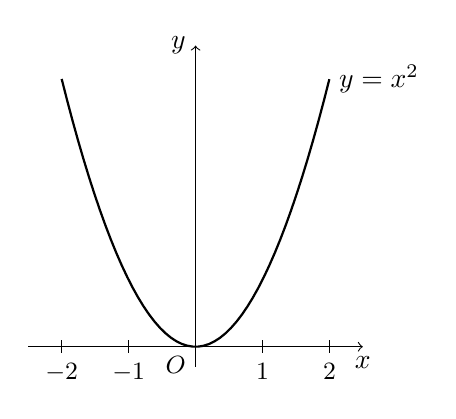
\begin{tikzpicture}[scale=0.85]
  \draw[->] (-2.5,0) -- (2.5,0) node[below] {$x$};
  \draw[->] (0,-0.3) -- (0,4.5) node[left] {$y$};
  \draw[thick, domain=-2:2, samples=50] plot (\x, {\x*\x});
  \node[right] at (2,4) {$y=x^2$};
  \foreach \x in {-2,-1,1,2} {
    \draw (\x,0.1) -- (\x,-0.1) node[below] {\small $\x$};
  }
  \node[below left] at (0,0) {\small $O$};
\end{tikzpicture}
\caption{}\label{fig:2.1.1}
\end{figure}

如果 $\forall x_{1}, x_{2} \in X, x_{1} \neq x_{2}$, 必有 $f(x_{1}) \neq f(x_{2})$, 即若 $f(x_{1})=f(x_{2})$, 必有 $x_{1}=x_{2}$, 则称 $f$ 为\textbf{单射}; 如果 $\forall y\in Y$, 必 $\exists x\in X$, s.t. $f(x)=y$, 则称 $f$ 为\textbf{满射}.

如果 $f$ 既为单射又为满射, 则称 $f$ 为\textbf{双射}或\textbf{一一映射}. 此时, $f$ 有逆映射 $f^{-1}\colon Y \to X$, $x = f^{-1}(y)$ (即 $y = f(x)$). 显然, 当 $f$ 为单射时, $f\colon X \to f(X)$ 就为双射或一一映射.

设 $X$ 为非空集合, $f\colon X \to \mathbb{R}$, $x \mapsto y = f(x)$ 为映射, 则称 $f$ 为\textbf{实(值)函数}, 本书中简称为\textbf{函数}.
\begin{itemize}
  \item 若 $X \subset \mathbb{R}$, 则称 $f$ 为一元(单变量)函数;
  \item 若 $X \subset \mathbb{R}^{2} = \{(x, y) \mid x, y \in \mathbb{R}\}$, 则称 $f$ 为二元函数;
  \item 若 $X \subset \mathbb{R}^{3} = \{(x, y, z) \mid x, y, z \in \mathbb{R}\}$, 则称 $f$ 为三元函数;
  \item 若 $X \subset \mathbb{R}^{n} = \{(x_{1}, x_{2}, \cdots, x_{n}) \mid x_{i} \in \mathbb{R}, i=1,2,\cdots,n\}$, 则称 $f$ 为 $n$ 元函数.
\end{itemize}

设 $f, g\colon X \to \mathbb{R}$, $x \in X$, 令
\begin{align*}
(f\pm g)(x) &= f(x)\pm g(x), \\
(fg)(x) &= f(x)g(x), \\
\frac{f}{g}(x) &= \frac{f(x)}{g(x)}\quad (g(x)\neq 0).
\end{align*}
它们分别定义了 $f$ 与 $g$ 的和函数 $f + g$, 差函数 $f - g$, 积函数 $fg$ 及商函数 $\frac{f}{g}$.

设 $f\colon X \to Y$, $g\colon Y \to Z$, 则称 $g \circ f\colon X \to Z$, $x \mapsto z = g \circ f(x) = g(f(x))$ 为 $f$ 与 $g$ 的复合. 两个函数 $f, g$ 的复合称为 $f$ 与 $g$ 的复合函数(如图~\ref{fig:2.1.2} 所示). 关于复合显然有 $(g \circ f) \circ h = g \circ (f \circ h)$.

\begin{figure}[htbp]
\centering
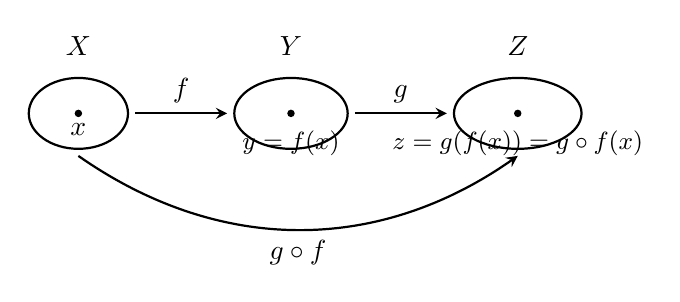
\begin{tikzpicture}[scale=0.9, >=stealth]
  \draw[thick] (0,0) ellipse (0.7cm and 0.5cm) node[above=0.6cm] {$X$};
  \fill (0,0) circle (1.5pt) node[below] {$x$};
  
  \draw[thick] (3.0,0) ellipse (0.8cm and 0.5cm) node[above=0.6cm] {$Y$};
  \fill (3.0,0) circle (1.5pt) node[below=0.1cm] {\small $y=f(x)$};
  
  \draw[thick] (6.2,0) ellipse (0.9cm and 0.5cm) node[above=0.6cm] {$Z$};
  \fill (6.2,0) circle (1.5pt) node[below=0.1cm] {\small $z=g(f(x))=g\circ f(x)$};
  
  \draw[->, thick] (0.8,0) -- (2.1,0) node[midway, above] {$f$};
  \draw[->, thick] (3.9,0) -- (5.2,0) node[midway, above] {$g$};
  \draw[->, thick] (0,-0.6) to[out=-35,in=-145] node[midway, below] {$g\circ f$} (6.2,-0.6);
\end{tikzpicture}
\caption{}\label{fig:2.1.2}
\end{figure}

中学里已学的基本初等函数共有 6 类:

(1) \textbf{常值函数} $y=f(x)=c$, 定义域为 $\mathbb{R}$.

(2) \textbf{幂函数} $y = f(x) = x^{\alpha}$ ($\alpha$ 为实数). 当 $x > 0$ 时, 任何 $\alpha$ 都有意义; $x^{n}\ (n \in \mathbb{N})$ 的定义域为实数集 $\mathbb{R}$; $x^{-n}\ (n \in \mathbb{N})$ 的定义域为 $\mathbb{R} \setminus \{0\}$; $x^{\frac{1}{2}} = \sqrt{x}$ 的定义域为 $[0, +\infty)$; $x^{-\frac{1}{2}}$ 的定义域为 $(0, +\infty)$; $x^{\frac{1}{3}}$ 的定义域为 $\mathbb{R}$; $x^{-\frac{1}{3}}$ 的定义域为 $\mathbb{R} \setminus \{0\}$; 等等.

(3) \textbf{三角函数} $y=\sin x, \cos x$ 定义域都为 $\mathbb{R}$; $y=\tan x$, 定义域为 $\mathbb{R} \setminus \{k\pi + \frac{\pi}{2}, k \in \mathbb{Z}\}$; $y=\cot x$, 定义域为 $\mathbb{R} \setminus \{k\pi, k \in \mathbb{Z}\}$; $y=\sec x$, 定义域为 $\mathbb{R} \setminus \{k\pi + \frac{\pi}{2}, k \in \mathbb{Z}\}$; $y=\csc x$, 定义域为 $\mathbb{R} \setminus \{k\pi, k \in \mathbb{Z}\}$.

(4) \textbf{反三角函数} $y=\arcsin x, \arccos x$ 定义域为 $[-1,1]$; $y=\arctan x, \operatorname{arccot} x$ 定义域为 $\mathbb{R}$.

(5) \textbf{指数函数} $y=a^{x}\ (a>0,a\neq1)$, 定义域为 $\mathbb{R}$.

(6) \textbf{对数函数} $y=\log_{a}x\ (a>0,a\neq1)$, 定义域为 $(0,+\infty)$. 特别地, 常用对数记作 $\lg x = \log_{10}x$, 自然对数记作 $\ln x = \log_{\mathrm{e}}x$.

读者应记住每个基本初等函数的值域, 并画出相应的图形.

\begin{definition}\label{def:2.1.2}
由基本初等函数通过有限次 $+$, $-$, $\cdot$, $\div$ 和复合得到的函数称为\textbf{初等函数}. 这是一类重要的函数.
\end{definition}

再给出几类今后要常用的函数.

\begin{example}\label{ex:2.1.1}
证明:
\begin{enumerate}[label=(\arabic*)]
  \item 双曲函数:
  \begin{align*}
  \sinh x &= \frac{e^{x}-e^{-x}}{2},\quad \cosh x=\frac{e^{x}+e^{-x}}{2}, \\
  \tanh x &= \frac{\sinh x}{\cosh x}=\frac{e^{x}-e^{-x}}{e^{x}+e^{-x}},\quad \coth x=\frac{\cosh x}{\sinh x}=\frac{e^{x}+e^{-x}}{e^{x}-e^{-x}}
\end{align*}
  都是初等函数. 读者经过验算可知双曲函数具有性质:
  \[
  \sinh 2x=2\sinh x\cosh x,\quad \cosh 2x=\cosh^{2}x+\sinh^{2}x,\quad \cosh^{2}x-\sinh^{2}x=1.
\]
  \item $y=\ln(x+\sqrt{x^{2}+1})$ 为初等函数.
  \item $y=|x|=\begin{cases} x, & x\geqslant0, \\ -x, & x<0 \end{cases}$ 为初等函数.
  \item 多项式函数 $y = a_{0}x^{n} + a_{1}x^{n-1} + \cdots + a_{n-1}x + a_{n}\ (a_{0} \neq 0)$ 与有理函数
  \[
  y = \frac{a_{0}x^{n} + a_{1}x^{n-1} + \cdots + a_{n-1}x + a_{n}}{b_{0}x^{m} + b_{1}x^{m-1} + \cdots + b_{m-1}x + b_{m}}\quad (a_{0} \neq 0, b_{0} \neq 0)
\]
  均为初等函数.
\end{enumerate}
\end{example}

\begin{proof}
(1) 以 $y = \tanh x$ 为例证明双曲函数为初等函数. 因为 $y = \tanh x = \frac{e^{x} - e^{-x}}{e^{x} + e^{-x}}$ 为基本初等函数 $e^{x}, e^{-x} = (e^{-1})^{x}$ 通过一次减法、一次加法、一次除法得到, 所以它为初等函数. 或者因为 $y = \tanh x = \frac{e^{x} - \frac{1}{e^{x}}}{e^{x} + \frac{1}{e^{x}}}$ 为基本初等函数 $e^{x}, 1$ 通过一次减法, 一次加法, 三次除法得到, 所以它为初等函数. 其他类似证明.

(2) 因为 $y=\ln(x+\sqrt{x^{2}+1})$ 由基本初等函数 $x, x^{2}, 1, \sqrt{x}, \ln x$ 通过两次加法, 两次复合得到, 所以它为初等函数.

(3) 因为 $y=|x|=\sqrt{x^{2}}$ 为基本初等函数 $x^{2}, \sqrt{x}$ 通过一次复合得到, 所以它为初等函数.

(4) 因为多项式函数 $y=a_{0}x^{n}+\cdots+a_{n}$ 为基本初等函数 $a_{0}, \cdots, a_{n}, x, \cdots, x^{n}$ 通过 $n$ 次乘法与 $n$ 次加法得到, 所以它为初等函数.

而有理函数为基本初等函数通过有限次乘法、加法以及除法得到, 所以它为初等函数.
\end{proof}

\begin{example}\label{ex:2.1.2}
\begin{enumerate}[label=(\arabic*)]
  \item 设 $f_{1}, f_{2}, \cdots, f_{n}$ 都为初等函数, 则由 $f_{1}, f_{2}, \cdots, f_{n}$ 经有限次 $+$, $-$, $\cdot$, $\div$, 复合运算得到的函数 $f$ 仍为初等函数.
  \item 设 $f, g$ 都为初等函数, 则 $\max\{f, g\}$ 与 $\min\{f, g\}$ 均为初等函数.
\end{enumerate}
\end{example}

\begin{proof}
(1) 因为 $f_{1}, f_{2}, \cdots, f_{n}$ 都为初等函数, 所以它们都由基本初等函数通过有限次 $+$, $-$, $\cdot$, $\div$, 复合运算得到. 从而, 由 $f_{1}, f_{2}, \cdots, f_{n}$ 经有限次 $+$, $-$, $\cdot$, $\div$, 复合运算得到的函数 $f$ 也由基本初等函数通过有限次 $+$, $-$, $\cdot$, $\div$, 复合运算得到, 该函数 $f$ 应是初等函数.

(2) 由 $f, g$ 都为初等函数及
\begin{align*}
\max\{f,g\} &= \frac{(f+g)+|f-g|}{2}=\frac{(f+g)+\sqrt{(f-g)^2}}{2}, \\
\min\{f,g\} &= \frac{(f+g)-|f-g|}{2}=\frac{(f+g)-\sqrt{(f-g)^2}}{2}
\end{align*}
或 $\min\{f,g\} = -\max\{-f,-g\}$ 可知 $\max\{f,g\}$ 与 $\min\{f,g\}$ 均为初等函数.
\end{proof}

另一类重要的函数就是\textbf{分段函数}, 即每一段上用不同的式子表达的函数.

\begin{example}\label{ex:2.1.3}
\begin{enumerate}[label=(\arabic*)]
  \item \textbf{符号函数}(如图~\ref{fig:2.1.3} 所示):
  \[
  y=\operatorname{sgn} x=\begin{cases}
  1, & x>0, \\
  0, & x=0, \\
  -1, & x<0.
\end{cases}
\]
  \item \textbf{“取整数”函数}(如图~\ref{fig:2.1.4} 所示):
  \[
  y=\lfloor x\rfloor = [x]
\]
  为不大于 $x$ 的最大整数, 此时有 $x-1<[x]\leqslant x<[x]+1$.
\end{enumerate}
\end{example}

\begin{figure}[htbp]
\centering
\begin{minipage}[t]{0.45\textwidth}
\centering
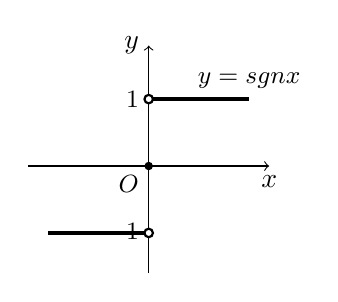
\begin{tikzpicture}[scale=0.85]
  \draw[->] (-1.8,0) -- (1.8,0) node[below] {$x$};
  \draw[->] (0,-1.6) -- (0,1.8) node[left] {$y$};
  \node[below left] at (0,0) {\small $O$};
  \draw[very thick] (0,1) -- (1.5,1) node[above, font=\small] {$y=\operatorname{sgn} x$};
  \draw[very thick] (-1.5,-1) -- (0,-1);
  \filldraw[fill=white, draw=black, thick] (0,1) circle (1.8pt);
  \filldraw[fill=white, draw=black, thick] (0,-1) circle (1.8pt);
  \fill (0,0) circle (1.8pt);
  \node[left] at (0,1) {\small $1$};
  \node[left] at (0,-1) {\small $-1$};
\end{tikzpicture}
\caption{}\label{fig:2.1.3}
\end{minipage}
\hfill
\begin{minipage}[t]{0.45\textwidth}
\centering
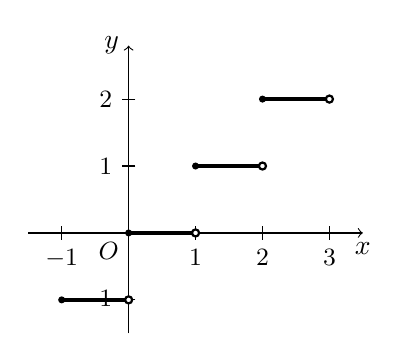
\begin{tikzpicture}[scale=0.85]
  \draw[->] (-1.5,0) -- (3.5,0) node[below] {$x$};
  \draw[->] (0,-1.5) -- (0,2.8) node[left] {$y$};
  \node[below left] at (0,0) {\small $O$};
  \foreach \x in {-1,1,2,3} {
    \draw (\x,0.1) -- (\x,-0.1) node[below] {\small $\x$};
  }
  \foreach \y in {-1,1,2} {
    \draw (0.1,\y) -- (-0.1,\y) node[left] {\small $\y$};
  }
  \draw[very thick] (-1,-1) -- (0,-1);
  \fill (-1,-1) circle (1.5pt);
  \filldraw[fill=white, draw=black, thick] (0,-1) circle (1.5pt);
  
  \draw[very thick] (0,0) -- (1,0);
  \fill (0,0) circle (1.5pt);
  \filldraw[fill=white, draw=black, thick] (1,0) circle (1.5pt);
  
  \draw[very thick] (1,1) -- (2,1);
  \fill (1,1) circle (1.5pt);
  \filldraw[fill=white, draw=black, thick] (2,1) circle (1.5pt);
  
  \draw[very thick] (2,2) -- (3,2);
  \fill (2,2) circle (1.5pt);
  \filldraw[fill=white, draw=black, thick] (3,2) circle (1.5pt);
\end{tikzpicture}
\caption{}\label{fig:2.1.4}
\end{minipage}
\end{figure}

\begin{enumerate}[label=(\arabic*), resume]
  \item \textbf{尾数函数}(如图~\ref{fig:2.1.5} 所示):
  \[
  y=x-[x]\overset{\mathrm{def}}{=}\{x\},
\]
  则 $0\leqslant\{x\}<1$, 且 $\{x\}$ 是以 $1$ 为周期的函数.
  \item \textbf{绝对值函数}(如图~\ref{fig:2.1.6} 所示):
  \[
  y=|x|=\begin{cases}
  x, & x\geqslant0, \\
  -x, & x<0.
\end{cases}
\]
  \item 设 $A \subseteq \mathbb{R}$, $A$ 的\textbf{特征函数} $\chi_{A}\colon \mathbb{R} \to \mathbb{R}$,
  \[
  \chi_{A}(x)=\begin{cases}
  1, & x\in A, \\
  0, & x\in\mathbb{R}\setminus A\ (\text{即 } x\notin A).
\end{cases}
\]
  \item \textbf{Dirichlet 函数}:
  \[
  D(x)=\begin{cases}
  1, & x\in\mathbb{Q}, \\
  0, & x\in\mathbb{R}\setminus\mathbb{Q},
\end{cases}
\]
  它是 $\mathbb{Q}$ 的特征函数.
\end{enumerate}

以上 6 个函数都为分段函数.

\begin{figure}[htbp]
\centering
\begin{minipage}[t]{0.45\textwidth}
\centering
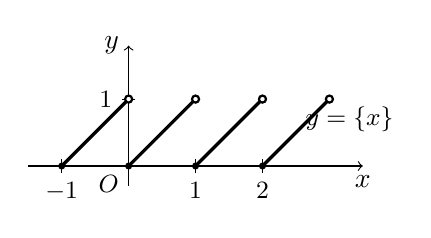
\begin{tikzpicture}[scale=0.85]
  \draw[->] (-1.5,0) -- (3.5,0) node[below] {$x$};
  \draw[->] (0,-0.3) -- (0,1.8) node[left] {$y$};
  \node[below left] at (0,0) {\small $O$};
  \draw (0.1,1) -- (-0.1,1) node[left] {\small $1$};
  \foreach \x in {-1,1,2} {
    \draw (\x,0.1) -- (\x,-0.1) node[below] {\small $\x$};
  }
  \foreach \k in {-1,0,1,2} {
    \draw[very thick] (\k,0) -- (\k+1,1);
    \fill (\k,0) circle (1.5pt);
    \filldraw[fill=white, draw=black, thick] (\k+1,1) circle (1.5pt);
  }
  \node[right, font=\small] at (2.5,0.7) {$y=\{x\}$};
\end{tikzpicture}
\caption{}\label{fig:2.1.5}
\end{minipage}
\hfill
\begin{minipage}[t]{0.45\textwidth}
\centering
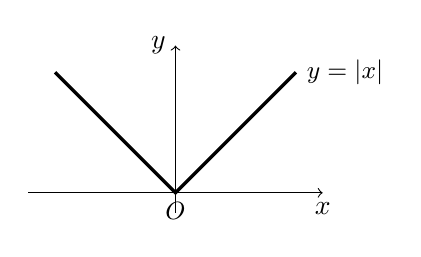
\begin{tikzpicture}[scale=0.85]
  \draw[->] (-2.2,0) -- (2.2,0) node[below] {$x$};
  \draw[->] (0,-0.3) -- (0,2.2) node[left] {$y$};
  \node[below] at (0,0) {\small $O$};
  \draw[very thick] (-1.8,1.8) -- (0,0) -- (1.8,1.8) node[right, font=\small] {$y=|x|$};
\end{tikzpicture}
\caption{}\label{fig:2.1.6}
\end{minipage}
\end{figure}

回想一下数列极限 $\lim\limits_{n\to+\infty}a_n=\lim\limits_{n\to+\infty}f(n)=a\in\mathbb{R}$ (收敛), $+\infty, -\infty, \infty$, 共有 4 种. 用 $N$ 刻画 $n$ 趋于 $+\infty$ 的程度, 用 $\varepsilon>0$ 刻画 $a_n$ 靠近 $a$ 的程度, 用 $A$ 刻画 $a_n$ 趋于 $+\infty, -\infty, \infty$ 的程度. 这里自变量只有一个趋向 $n\to+\infty$, 而一般函数 $f(x)$ 除了 $x\to+\infty$ 外, 还有 $x\to x_0, x_0^+, x_0^-, x\to-\infty, \infty$ 等情况.

我们考虑函数极限 $\lim\limits_{x \to x_{0}} f(x) = a \in \mathbb{R}$ (收敛), $+\infty, -\infty, \infty$ 时, 其中自变量趋向有 $x \to x_{0}, x \to x_{0}^{+}, x_{0}^{-}, +\infty, -\infty, \infty$ 共有 $6 \times 4 = 24$ 种不同情况, 我们用 $\delta > 0$ 刻画 $x$ 与 $x_{0}$ 或 $x$ 与 $x_{0}^{+}$ 或 $x$ 与 $x_{0}^{-}$ 的靠近程度, 用 $\Delta > 0$ 刻画 $x$ 趋于 $+\infty, -\infty, \infty$ 的程度, 用 $\varepsilon > 0$ 刻画 $f(x)$ 与 $a$ 靠近的程度, 用 $A$ 刻画 $f(x)$ 趋于 $+\infty, -\infty, \infty$ 的程度.

\begin{definition}\label{def:2.1.3}
设函数 $y = f(x)$ 在 $x_{0}$ 的一个去心开邻域 $(x_{0} - \delta_{0}, x_{0} + \delta_{0}) \setminus \{x_{0}\}$ 内有定义 ($x_{0}$ 处可以无定义). 如果有一数 $a \in \mathbb{R}$, s.t. $\forall \varepsilon > 0, \exists \delta \in (0, \delta_{0})$, 当 $0 < |x - x_{0}| < \delta$ 时, 有
\[
|f(x)-a|<\varepsilon,
\]
则称函数 $f(x)$ 在 $x_{0}$ 处(当 $x$ 趋于 $x_{0}$ 时)有极限 $a$, 记作 $\lim\limits_{x \to x_{0}} f(x) = a$, 或 $f(x) \to a\ (x \to x_{0})$ (如图~\ref{fig:2.1.7} 所示).

设函数 $y = f(x)$ 在 $x_{0}$ 去心右旁 $(x_{0}, x_{0} + \delta_{0})$ 有定义. 如果 $\forall A > 0, \exists \delta \in (0, \delta_{0})$, 当 $x_{0} < x < x_{0} + \delta$ 时, 有 $f(x) > A$, 则称函数 $f(x)$ 在 $x_{0}$ 的右旁(当 $x$ 趋于 $x_{0}^{+}$ 时)有右极限 $+\infty$, 记作 $f(x_{0} + 0) = f(x_{0}^{+}) = \lim\limits_{x \to x_{0}^{+}} f(x) = +\infty$, 或 $f(x) \to +\infty\ (x \to x_{0}^{+})$ (如图~\ref{fig:2.1.8} 所示).
\end{definition}

\begin{figure}[htbp]
\centering
\begin{minipage}[t]{0.45\textwidth}
\centering
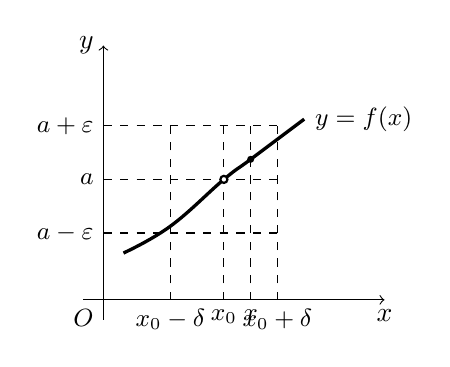
\begin{tikzpicture}[scale=0.85]
  \draw[->] (-0.3,0) -- (4.2,0) node[below] {$x$};
  \draw[->] (0,-0.3) -- (0,3.8) node[left] {$y$};
  \node[below left] at (0,0) {\small $O$};
  
  \draw[dashed] (1.0,0) node[below] {\small $x_0-\delta$} -- (1.0,2.6);
  \draw[dashed] (1.8,0) node[below] {\small $x_0$} -- (1.8,2.6);
  \draw[dashed] (2.2,0) node[below] {\small $x$} -- (2.2,2.6);
  \draw[dashed] (2.6,0) node[below] {\small $x_0+\delta$} -- (2.6,2.6);
  
  \draw[dashed] (0,1.0) node[left] {\small $a-\varepsilon$} -- (2.6,1.0);
  \draw[dashed] (0,1.8) node[left] {\small $a$} -- (2.6,1.8);
  \draw[dashed] (0,2.6) node[left] {\small $a+\varepsilon$} -- (2.6,2.6);
  
  \draw[very thick] plot [smooth, tension=0.7] coordinates {(0.3,0.7) (1.0,1.1) (1.8,1.8) (2.2,2.1) (3.0,2.7)} node[right, font=\small] {$y=f(x)$};
  \fill (2.2,2.1) circle (1.5pt);
  \filldraw[fill=white, draw=black, thick] (1.8,1.8) circle (1.5pt);
\end{tikzpicture}
\caption{}\label{fig:2.1.7}
\end{minipage}
\hfill
\begin{minipage}[t]{0.45\textwidth}
\centering
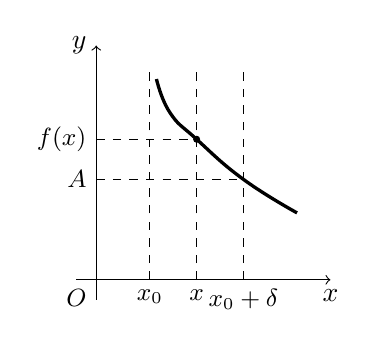
\begin{tikzpicture}[scale=0.85]
  \draw[->] (-0.3,0) -- (3.5,0) node[below] {$x$};
  \draw[->] (0,-0.3) -- (0,3.5) node[left] {$y$};
  \node[below left] at (0,0) {\small $O$};
  
  \draw[dashed] (0.8,0) node[below] {\small $x_0$} -- (0.8,3.2);
  \draw[dashed] (1.5,0) node[below] {\small $x$} -- (1.5,3.2);
  \draw[dashed] (2.2,0) node[below] {\small $x_0+\delta$} -- (2.2,3.2);
  
  \draw[dashed] (0,1.5) node[left] {\small $A$} -- (2.2,1.5);
  \draw[dashed] (0,2.1) node[left] {\small $f(x)$} -- (1.5,2.1);
  
  \draw[very thick] plot [smooth, tension=0.8] coordinates {(0.9,3.0) (1.1,2.5) (1.5,2.1) (2.2,1.5) (3.0,1.0)};
  \fill (1.5,2.1) circle (1.5pt);
\end{tikzpicture}
\caption{}\label{fig:2.1.8}
\end{minipage}
\end{figure}

设函数 $y = f(x)$ 在 $\infty$ 的开邻域 $(-\infty, -\Delta_{0}) \cup (\Delta_{0}, +\infty)$ 内有定义. 如果 $\forall A > 0, \exists \Delta > \Delta_{0} > 0$, 当 $|x| > \Delta$ 时, 有
\[
|f(x)|>A,
\]
则称函数 $y = f(x)$ 在 $\infty$ 处(当 $x \to \infty$ 时)有极限 $\infty$, 记作 $f(\infty) = \lim\limits_{x \to \infty} f(x) = \infty$ 或 $f(x) \to \infty\ (x \to \infty)$ (如图~\ref{fig:2.1.9} 所示).

设函数 $y = f(x)$ 在 $+\infty$ 的开邻域 $(\Delta_{0}, +\infty)$ 内有定义. 如果 $\forall \varepsilon > 0, \exists \Delta > \Delta_{0} > 0$, 当 $x > \Delta$ 时, 有
\[
|f(x)-a|<\varepsilon,
\]
则称函数 $y = f(x)$ 在 $+\infty$ 处(当 $x \to +\infty$ 时)有极限 $a$, 记作 $\lim\limits_{x \to +\infty} f(x) = a$ 或 $f(x) \to a\ (x \to +\infty)$ (如图~\ref{fig:2.1.10} 所示).

\begin{figure}[htbp]
\centering
\begin{minipage}[t]{0.45\textwidth}
\centering
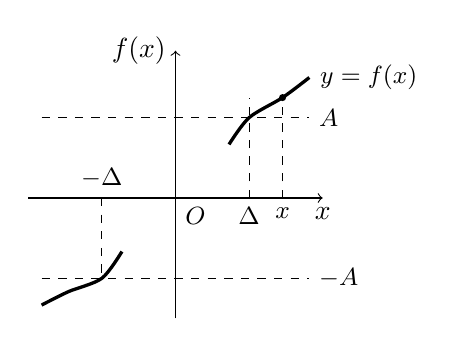
\begin{tikzpicture}[scale=0.85]
  \draw[->] (-2.2,0) -- (2.2,0) node[below] {$x$};
  \draw[->] (0,-1.8) -- (0,2.2) node[left] {$f(x)$};
  \node[below right] at (0,0) {\small $O$};
  
  \draw[dashed] (1.1,0) node[below] {\small $\Delta$} -- (1.1,1.5);
  \draw[dashed] (1.6,0) node[below] {\small $x$} -- (1.6,1.5);
  \draw[dashed] (-1.1,0) node[above] {\small $-\Delta$} -- (-1.1,-1.2);
  
  \draw[dashed] (-2,1.2) -- (2,1.2) node[right] {\small $A$};
  \draw[dashed] (-2,-1.2) -- (2,-1.2) node[right] {\small $-A$};
  
  \draw[very thick] plot [smooth] coordinates {(0.8,0.8) (1.1,1.2) (1.6,1.5) (2.0,1.8)} node[right, font=\small] {$y=f(x)$};
  \draw[very thick] plot [smooth] coordinates {(-2.0,-1.6) (-1.6,-1.4) (-1.1,-1.2) (-0.8,-0.8)};
  \fill (1.6,1.5) circle (1.5pt);
\end{tikzpicture}
\caption{}\label{fig:2.1.9}
\end{minipage}
\hfill
\begin{minipage}[t]{0.45\textwidth}
\centering
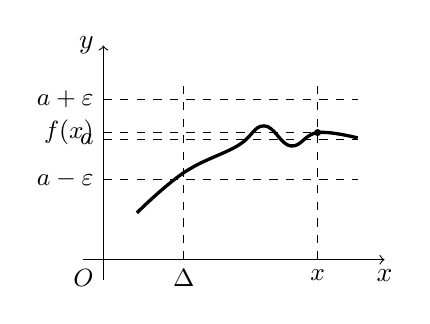
\begin{tikzpicture}[scale=0.85]
  \draw[->] (-0.3,0) -- (4.2,0) node[below] {$x$};
  \draw[->] (0,-0.3) -- (0,3.2) node[left] {$y$};
  \node[below left] at (0,0) {\small $O$};
  
  \draw[dashed] (1.2,0) node[below] {\small $\Delta$} -- (1.2,2.6);
  \draw[dashed] (3.2,0) node[below] {\small $x$} -- (3.2,2.6);
  
  \draw[dashed] (0,1.2) node[left] {\small $a-\varepsilon$} -- (3.8,1.2);
  \draw[dashed] (0,1.8) node[left] {\small $a$} -- (3.8,1.8);
  \draw[dashed] (0,2.4) node[left] {\small $a+\varepsilon$} -- (3.8,2.4);
  \draw[dashed] (0,1.9) node[left] {\small $f(x)$} -- (3.2,1.9);
  
  \draw[very thick] plot [smooth, tension=0.7] coordinates {(0.5,0.7) (1.2,1.3) (2.0,1.7) (2.4,2.0) (2.8,1.7) (3.2,1.9) (3.8,1.82)};
  \fill (3.2,1.9) circle (1.5pt);
\end{tikzpicture}
\caption{}\label{fig:2.1.10}
\end{minipage}
\end{figure}

其余 20 种情形读者自行叙述, 并配出相应的示意图.

\begin{theorem}\label{thm:2.1.1}
$\lim\limits_{x \to x_0} f(x) = a \iff f(x_0^+) = \lim\limits_{x \to x_0^+} f(x) = a = \lim\limits_{x \to x_0^-} f(x) = f(x_0^-)$, 其中 $a$ 为实数, $+\infty, -\infty, \infty$.
\end{theorem}

\begin{proof}
($\Rightarrow$) 显然.

($\Leftarrow$) 对于 $a$ 的任何开邻域 $U(a)$, 因 $\lim\limits_{x\to x_0^+}f(x)=a$, 故 $\exists\delta_1>0$, 当 $x_0<x<x_0+\delta_1$ 时, $f(x)\in U(a)$. 因为 $\lim\limits_{x\to x_0^-}f(x)=a$, 所以 $\exists\delta_2>0$, 当 $x_0-\delta_2<x<x_0$ 时, $f(x)\in U(a)$.

因此, 取 $\delta = \min\{\delta_1, \delta_2\}$, 当 $0 < |x - x_0| < \delta$ 时, 有 $f(x) \in U(a)$. 于是,
\[
\lim_{x\to x_{0}}f(x)=a.
\]
\end{proof}

\begin{theorem}\label{thm:2.1.2}
$\lim\limits_{x\to\infty}f(x)=a \iff \lim\limits_{x\to+\infty}f(x)=a$ 且 $\lim\limits_{x\to-\infty}f(x)=a$, 其中 $a$ 为实数, $+\infty, -\infty, \infty$.
\end{theorem}

\begin{proof}
($\Rightarrow$) 对 $a$ 的任何开邻域 $U(a)$, 因 $\lim\limits_{x\to\infty}f(x)=a$, 故 $\exists\Delta>0$, 当 $|x|>\Delta$ 时, 必有 $f(x)\in U(a)$. 于是, 当 $x>\Delta$ 时, 有 $f(x)\in U(a)$, 从而 $\lim\limits_{x\to+\infty}f(x)=a$; 当 $x < -\Delta$ 时, 有 $f(x) \in U(a)$, 从而 $\lim\limits_{x\to-\infty} f(x) = a$.

($\Leftarrow$) 由 $\lim\limits_{x\to+\infty}f(x)=a$, 故对 $a$ 的任何开邻域 $U(a)$, $\exists\Delta_{1}>0$, 当 $x>\Delta_{1}$ 时, 有 $f(x)\in U(a)$. 再由 $\lim\limits_{x\to-\infty}f(x)=a$, 故对 $a$ 的任何开邻域 $U(a)$, $\exists\Delta_{2}>0$, 当 $x<-\Delta_{2}$ 时, 有 $f(x)\in U(a)$. 因此当 $|x|>\Delta=\max\{\Delta_{1},\Delta_{2}\}$ 时, $f(x)\in U(a)$, 从而 $\lim\limits_{x\to\infty}f(x)=a$.
\end{proof}

\begin{theorem}[归结原则, Heine]\label{thm:2.1.3}
函数 $y = f(x)$, 其定义域为 $x_{0}$ 的去心开邻域 $U^{\circ}(x_{0})$, 则在 $U^{\circ}(x_{0})$ 中有
\[
\lim_{x\to x_0}f(x)=a \iff \forall \{x_n\}\subset U^\circ(x_0),\ x_n\to x_0\ (n\to+\infty),\text{ 必有 } \lim_{n\to+\infty}f(x_n)=a,
\]
其中 $a$ 为实数, $+\infty, -\infty, \infty$; $x_0$ 可换为 $x_0^+, x_0^-, +\infty, -\infty, \infty$.
\end{theorem}

\begin{proof}
先证 $a \in \mathbb{R}, x_0 \in \mathbb{R}$ 的情形.

($\Rightarrow$) $\forall\varepsilon>0$, 因为 $\lim\limits_{x\to x_0}f(x)=a$, 所以 $\exists\delta>0$, 当 $0<|x-x_0|<\delta$ 时, $|f(x)-a|<\varepsilon$. 而由于 $\forall x_n\neq x_0, x_n\to x_0\ (n\to+\infty)$, 所以对取定的 $\delta>0$, $\exists N\in\mathbb{N}$, 当 $n>N$ 时, 有 $0<|x_n-x_0|<\delta$, 所以
\[
|f(x_{n})-a|<\varepsilon,
\]
即 $\lim\limits_{n\to+\infty}f(x_{n})=a$.

($\Leftarrow$) (反证)假设 $\lim\limits_{x \to x_0} f(x) \neq a$, 则 $\exists \varepsilon_0 > 0, \forall n \in \mathbb{N}$, $\exists x_n \neq x_0$, s.t. $0 < |x_n - x_0| < \frac{1}{n}$, 但
\[
|f(x_{n})-a|\geqslant\varepsilon_{0}.
\]
显然, $\lim\limits_{n\to+\infty} x_{n}=x_{0}$, 但由条件知,
\[
0=|a-a|=\lim_{n\to+\infty}|f(x_{n})-a|\geqslant\varepsilon_{0}>0,
\]
矛盾. 所以, $\lim\limits_{x\to x_0}f(x)=a$.

其他情形可类似证明.

统一描述如下:

($\Rightarrow$) 对 $a$ 的任何开邻域 $U(a)$, 因为 $\lim\limits_{x \to x_0} f(x) = a$, 存在 $x_0$ 的去心开邻域 $V^\circ(x_0)$, 当 $x \in V^\circ(x_0)$ 时, $f(x) \in U(a)$. 又因 $x_n \to x_0\ (n \to +\infty), x_n \neq x_0$, 故 $\exists N \in \mathbb{N}$, 当 $n > N$ 时, $x_n \in V^\circ(x_0)$, 从而 $f(x_n) \in U(a)$. 这就证明了 $\lim\limits_{n \to +\infty} f(x_n) = a$.

($\Leftarrow$) (反证)假设 $\lim\limits_{x\to x_0}f(x)\neq a$, 则存在 $a$ 的开邻域 $U_0(a)$, $\forall n\in\mathbb{N}$, $\exists x_n\neq x_0$, s.t. $x_n\in V^\circ_n(x_0)$ (6 种情形分别为 $(x_0-\frac{1}{n},x_0+\frac{1}{n})\setminus\{x_0\}$, $(x_0,x_0+\frac{1}{n})$, $(x_0-\frac{1}{n},x_0)$, $(n,+\infty)$, $(-\infty,-n)$, $(-\infty,-n)\cup(n,+\infty)$), 但是 $f(x_n)\notin U_0(a)$. 显然, $\lim\limits_{n\to+\infty}x_n=x_0$, 但 $\lim\limits_{n\to+\infty}f(x_n)\neq a$, 这与已知条件矛盾.
\end{proof}

\begin{theorem}[函数收敛的 Cauchy 准则]\label{thm:2.1.4}
设 $f$ 在 $x_{0}$ 的去心开邻域 $U^{\circ}(x_{0},\delta_{0})$ 内定义, 则 $\lim\limits_{x\to x_0} f(x)$ 存在有限 $\iff \forall\varepsilon>0,\exists\delta\in(0,\delta_{0})$, s.t. $\forall x^{\prime},x^{\prime\prime}\in U^{\circ}(x_{0},\delta)$, 有
\[
|f(x^{\prime})-f(x^{\prime \prime})|<\varepsilon.
\]
\end{theorem}

\begin{proof}
($\Rightarrow$) 设 $\lim\limits_{x\to x_0}f(x)=a\in\mathbb{R}$, 则 $\forall\varepsilon>0,\exists\delta\in(0,\delta_0)$, s.t. $\forall x\in U^\circ(x_0,\delta)$, 有 $|f(x)-a|<\frac{\varepsilon}{2}$. 于是, 对于 $\forall x',x''\in U^\circ(x_0,\delta)$, 有
\begin{align*}
|f(x^{\prime})-f(x^{\prime \prime})| &= |(f(x^{\prime})-a)-(f(x^{\prime \prime})-a)| \\
&\leqslant |f(x^{\prime})-a|+|f(x^{\prime \prime})-a| < \frac{\varepsilon}{2}+\frac{\varepsilon}{2}=\varepsilon.
\end{align*}

($\Leftarrow$) 设数列 $\{x_n\}\subset U^\circ(x_0,\delta_0)$, 且 $\lim\limits_{n\to+\infty}x_n=x_0$. 按已知条件, $\forall\varepsilon>0$, $\exists\delta\in(0,\delta_0)$, s.t. $\forall x',x''\in U^\circ(x_0,\delta)$, 有 $|f(x')-f(x'')|<\varepsilon$.

对上述的 $\delta$, 由于 $\lim\limits_{n\to+\infty}x_n=x_0$, 故 $\exists N\in\mathbb{N}$, 当 $n,m>N$ 时, 有 $x_n,x_m\in U^\circ(x_0,\delta)$. 从而, $|f(x_n)-f(x_m)|<\varepsilon$. 这表明了 $\{f(x_n)\}$ 为 Cauchy 数列. 根据数列的 Cauchy 准则知, $\{f(x_n)\}$ 收敛.

进一步考虑 $\{x_{n}^{\prime}\}\subset U^{\circ}(x_{0},\delta_{0})$, $\{x_{n}^{\prime\prime}\}\subset U^{\circ}(x_{0},\delta_{0})$, 且 $\lim\limits_{n\to+\infty}x_{n}^{\prime}=x_{0}=\lim\limits_{n\to+\infty}x_{n}^{\prime\prime}$. 构造交错数列 $\{x_n\}\colon x_{1}^{\prime}, x_{1}^{\prime\prime}, x_{2}^{\prime}, x_{2}^{\prime\prime}, \cdots, x_{k}^{\prime}, x_{k}^{\prime\prime}, \cdots$, 显然 $\{x_{n}\}\subset U^{\circ}(x_{0},\delta_{0})$, $\lim\limits_{n\to+\infty}x_{n}=x_{0}$. 由上述证明所得结果, $\{f(x_{n})\}$ 收敛, 从而
\[
\lim_{n\to+\infty}f(x_{n}^{\prime})=\lim_{n\to+\infty}f(x_{n})=\lim_{n\to+\infty}f(x_{n}^{\prime\prime}),
\]
记此公共极限为 $a$. 根据归结原则(定理~\ref{thm:2.1.3}), $\lim\limits_{x\to x_0}f(x)=a$.
\end{proof}

\begin{remark}\label{rem:2.1.1}
定理~\ref{thm:2.1.4} 等价于: $f(x)$ 在 $x_{0}$ 不存在有限极限 $\iff \exists \varepsilon_{0} > 0, \forall \delta > 0$, 总有 $x_{\delta}^{\prime}, x_{\delta}^{\prime\prime} \in U^{\circ}(x_{0}, \delta)$, s.t. $|f(x_{\delta}^{\prime}) - f(x_{\delta}^{\prime\prime})| \geqslant \varepsilon_{0}$.
\end{remark}

\begin{remark}\label{rem:2.1.2}
定理~\ref{thm:2.1.4} 与注~\ref{rem:2.1.1} 中, $x_{0}$ 换为 $x_{0}^{\pm}, \pm\infty, \infty$, 相应结论成立, 证明也类似.
\end{remark}

\begin{example}\label{ex:2.1.4}
设 $f(x) = c$ 为常值函数, 则 $\lim\limits_{x \to x_0} f(x) = c$, 其中 $x_0$ 或 $x_0^+, x_0^-, +\infty, -\infty, \infty$.
\end{example}

\begin{proof}
$\forall\varepsilon>0$, 任取 $\delta>0$, 当 $0<|x-x_{0}|<\delta$ 时, 有
\[
|f(x)-c|=|c-c|=0<\varepsilon,
\]
所以 $\lim\limits_{x\to x_0}f(x)=c$. 其他情形类似证明.
\end{proof}

\begin{example}\label{ex:2.1.5}
证明: $\lim\limits_{x\to+\infty}\frac{1}{x^\alpha}=0\ (\alpha>0)$.
\end{example}

\begin{proof}
$\forall\varepsilon>0$, 取 $\Delta>\left(\frac{1}{\varepsilon}\right)^{\frac{1}{\alpha}}$, 则当 $x>\Delta$ 时, 有
\[
\left|\frac{1}{x^{\alpha}}-0\right|=\frac{1}{x^{\alpha}}<\frac{1}{\Delta^{\alpha}}<\varepsilon,
\]
所以 $\lim\limits_{x\to+\infty}\frac{1}{x^{\alpha}}=0$.
\end{proof}

\begin{example}\label{ex:2.1.6}
证明:
\begin{enumerate}[label=(\arabic*)]
  \item $\lim\limits_{x\to-\infty}\arctan x=-\frac{\pi}{2}$;
  \item $\lim\limits_{x \to +\infty} \arctan x = \frac{\pi}{2}$.
\end{enumerate}
\end{example}

\begin{proof}
(1) $\forall\varepsilon>0$, 取 $\Delta>\tan\left(\frac{\pi}{2}-\varepsilon\right)$, 当 $x<-\Delta$ 时, 有
\[
-\frac{\pi}{2}-\varepsilon<-\frac{\pi}{2}<\arctan x<\arctan(-\Delta)=-\left(\frac{\pi}{2}-\varepsilon\right)<-\frac{\pi}{2}+\varepsilon,
\]
因此 $\lim\limits_{x\to-\infty}\arctan x=-\frac{\pi}{2}$.

(2) $\forall\varepsilon>0$, 取 $\Delta>\tan\left(\frac{\pi}{2}-\varepsilon\right)=\cot\varepsilon$, 当 $x>\Delta$ 时, 有
\[
\frac{\pi}{2}-\varepsilon < \arctan\Delta < \arctan x < \frac{\pi}{2} < \frac{\pi}{2}+\varepsilon,
\]
所以 $\lim\limits_{x\to+\infty}\arctan x=\frac{\pi}{2}$ (如图~\ref{fig:2.1.11} 所示).
\end{proof}

\begin{figure}[htbp]
\centering
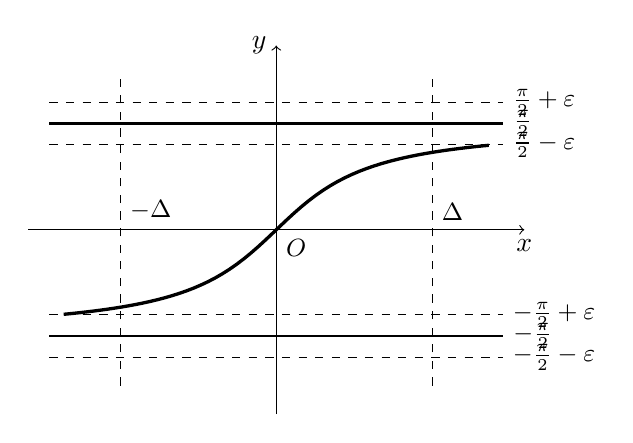
\begin{tikzpicture}[scale=0.9]
  \draw[->] (-3.5,0) -- (3.5,0) node[below] {$x$};
  \draw[->] (0,-2.6) -- (0,2.6) node[left] {$y$};
  \node[below right] at (0,0) {\small $O$};
  
  \draw[thick] (-3.2,1.5) -- (3.2,1.5) node[right] {\small $\frac{\pi}{2}$};
  \draw[thick] (-3.2,-1.5) -- (3.2,-1.5) node[right] {\small $-\frac{\pi}{2}$};
  
  \draw[dashed] (-3.2,1.8) -- (3.2,1.8) node[right] {\small $\frac{\pi}{2}+\varepsilon$};
  \draw[dashed] (-3.2,1.2) -- (3.2,1.2) node[right] {\small $\frac{\pi}{2}-\varepsilon$};
  \draw[dashed] (-3.2,-1.2) -- (3.2,-1.2) node[right] {\small $-\frac{\pi}{2}+\varepsilon$};
  \draw[dashed] (-3.2,-1.8) -- (3.2,-1.8) node[right] {\small $-\frac{\pi}{2}-\varepsilon$};
  
  \draw[dashed] (2.2,-2.2) -- (2.2,2.2);
  \node[above right] at (2.2,0) {\small $\Delta$};
  \draw[dashed] (-2.2,-2.2) -- (-2.2,2.2);
  \node[above right] at (-2.2,0) {\small $-\Delta$};
  
  \draw[very thick, domain=-3:3, samples=60] plot (\x, {1.5*(2/pi)*rad(atan(\x))});
\end{tikzpicture}
\caption{}\label{fig:2.1.11}
\end{figure}

\begin{example}\label{ex:2.1.7}
证明: $\lim\limits_{x\to2}\frac{x^{2}-4}{x-2}=\lim\limits_{x\to2}(x+2)=4$.
\end{example}

\begin{proof}
$\forall\varepsilon>0$, 取 $\delta=\varepsilon$, 当 $0<|x-2|<\delta=\varepsilon$ 时, 有
\[
\left|\frac{x^{2}-4}{x-2}-4\right|=|(x+2)-4|=|x-2|<\delta=\varepsilon,
\]
因此 $\lim\limits_{x\to2}\frac{x^{2}-4}{x-2}=4$.
\end{proof}

函数 $y=\frac{x^{2}-4}{x-2}$ 和 $y=x+2$ 的定义域不同, 前者为 $\mathbb{R}\setminus\{2\}$, 后者为 $\mathbb{R}$, 但它们在 $x\to2$ 时有相同的极限, 这是因为在考虑 $x\to x_{0}$ 的极限时, 并不要求函数在 $x=x_{0}$ 处有定义或函数在 $x_{0}$ 处的值是多少. 下面的例子也是如此.

\begin{example}\label{ex:2.1.8}
证明: $\lim\limits_{x\to1}\frac{x^{2}-1}{2x^{2}-x-1}=\lim\limits_{x\to1}\frac{x+1}{2x+1}=\frac{2}{3}$.
\end{example}

\begin{proof}
$\forall\varepsilon>0$, 取 $\delta=\min\{1,3\varepsilon\}$ (如图~\ref{fig:2.1.12} 所示), 当 $0<|x-1|<\delta$ 时, 有
\[
\left|\frac{x^2-1}{2x^2-x-1}-\frac{2}{3}\right|=\left|\frac{x+1}{2x+1}-\frac{2}{3}\right|=\frac{|x-1|}{3|2x+1|}<\frac{\delta}{3}\leqslant\varepsilon,
\]
所以 $\lim\limits_{x\to1}\frac{x^{2}-1}{2x^{2}-x-1}=\frac{2}{3}$.
\end{proof}

\begin{remark}\label{rem:2.1.3}
为了使得 $|2x+1|\geqslant1$, 我们先限制 $|x-1|<1\iff 0<x<2$. 再由 $\frac{\delta}{3}\leqslant\varepsilon$ 解得 $\delta\leqslant3\varepsilon$, 所以取 $\delta=\min\{1,3\varepsilon\}$.

如果先限制 $|x-1| < \frac{1}{2} \iff -\frac{1}{2} < x-1 < \frac{1}{2} \iff \frac{1}{2} < x < \frac{3}{2}$ (如图~\ref{fig:2.1.13} 所示). 于是, $|2x+1| \geqslant |2 \cdot \frac{1}{2}+1| = 2$, 从而
\[
\left|\frac{x^{2}-1}{2x^{2}-x-1}-\frac{2}{3}\right|=\frac{|x-1|}{3|2x+1|}<\frac{\delta}{3\cdot2}=\frac{\delta}{6}\leqslant\varepsilon,
\]
只需取 $\delta = \min\left\{\frac{1}{2},6\varepsilon\right\}$.
\end{remark}

\begin{figure}[htbp]
\centering
\begin{minipage}[t]{0.45\textwidth}
\centering
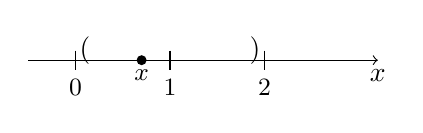
\begin{tikzpicture}[scale=1.2]
  \draw[->] (-0.5,0) -- (3.2,0) node[below] {$x$};
  \draw (0,0.1) -- (0,-0.1) node[below] {\small $0$};
  \draw (1,0.1) -- (1,-0.1) node[below] {\small $1$};
  \draw (2,0.1) -- (2,-0.1) node[below] {\small $2$};
  \node at (0.1,0.1) {$($};
  \node at (1.9,0.1) {$)$};
  \fill (0.7,0) circle (1.5pt) node[below] {\small $x$};
\end{tikzpicture}
\caption{}\label{fig:2.1.12}
\end{minipage}
\hfill
\begin{minipage}[t]{0.45\textwidth}
\centering
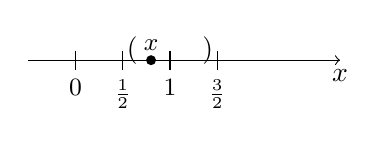
\begin{tikzpicture}[scale=1.2]
  \draw[->] (-0.5,0) -- (2.8,0) node[below] {$x$};
  \draw (0,0.1) -- (0,-0.1) node[below] {\small $0$};
  \draw (0.5,0.1) -- (0.5,-0.1) node[below] {\small $\frac{1}{2}$};
  \draw (1,0.1) -- (1,-0.1) node[below] {\small $1$};
  \draw (1.5,0.1) -- (1.5,-0.1) node[below] {\small $\frac{3}{2}$};
  \node at (0.6,0.1) {$($};
  \node at (1.4,0.1) {$)$};
  \fill (0.8,0) circle (1.5pt) node[above] {\small $x$};
\end{tikzpicture}
\caption{}\label{fig:2.1.13}
\end{minipage}
\end{figure}

\begin{example}\label{ex:2.1.9}
证明:
\begin{enumerate}[label=(\arabic*)]
  \item $\lim\limits_{x\to1^{+}}\frac{x^{2}+1}{x^{2}-1}=+\infty$;
  \item $\lim\limits_{x \to 1^-} \frac{x^2 + 1}{x^2 - 1} = -\infty$.
\end{enumerate}
\end{example}

\begin{proof}
(1) $\forall A>0$, 取 $\delta=\min\left\{1,\frac{1}{3A}\right\}$ (如图~\ref{fig:2.1.14} 所示), 当 $1<x<1+\delta$ 时, 有
\[
\frac{x^{2}+1}{x^{2}-1}=\frac{x^{2}+1}{(x+1)(x-1)}>\frac{1}{(2+1)\delta}=\frac{1}{3\delta}\geqslant A,
\]
所以 $\lim\limits_{x\to1^{+}}\frac{x^{2}+1}{x^{2}-1}=+\infty$.

(2) $\forall A>0$, 取 $\delta=\min\left\{1,\frac{1}{2A}\right\}$ (如图~\ref{fig:2.1.15} 所示), 当 $1-\delta<x<1$ 时, 有
\[
\frac{x^{2}+1}{x^{2}-1}=\frac{x^{2}+1}{(x+1)(x-1)}=-\frac{x^{2}+1}{(x+1)(1-x)}<-\frac{1}{2\delta}<-A,
\]
因此 $\lim\limits_{x\to1^{-}}\frac{x^{2}+1}{x^{2}-1}=-\infty$.
\end{proof}

\begin{figure}[htbp]
\centering
\begin{minipage}[t]{0.45\textwidth}
\centering
\begin{tikzpicture}[scale=1.2]
  \draw[->] (-0.5,0) -- (3.2,0) node[below] {$x$};
  \draw (0,0.1) -- (0,-0.1) node[below] {\small $0$};
  \draw (1,0.1) -- (1,-0.1) node[below] {\small $1$};
  \draw (2,0.1) -- (2,-0.1) node[below] {\small $2$};
  \node at (1.8,0.1) {$)$};
  \fill (1.4,0) circle (1.5pt) node[below] {\small $x$};
\end{tikzpicture}
\caption{}\label{fig:2.1.14}
\end{minipage}
\hfill
\begin{minipage}[t]{0.45\textwidth}
\centering
\begin{tikzpicture}[scale=1.2]
  \draw[->] (-0.5,0) -- (3.2,0) node[below] {$x$};
  \draw (0,0.1) -- (0,-0.1) node[below] {\small $0$};
  \draw (1,0.1) -- (1,-0.1) node[below] {\small $1$};
  \draw (2,0.1) -- (2,-0.1) node[below] {\small $2$};
  \node at (0.2,0.1) {$($};
  \fill (0.7,0) circle (1.5pt) node[below] {\small $x$};
\end{tikzpicture}
\caption{}\label{fig:2.1.15}
\end{minipage}
\end{figure}

\begin{example}\label{ex:2.1.10}
证明 $\lim\limits_{x\to0}x^{\alpha}\sin\frac{1}{x}=0\ (\alpha>0)$ (如图~\ref{fig:2.1.16} 所示).
\end{example}

\begin{proof}
$\forall\varepsilon>0$, 取 $\delta=\varepsilon^{\frac{1}{\alpha}}$, 当 $0<|x-0|<\delta$ 时, 有
\[
\left|x^{\alpha}\sin\frac{1}{x}-0\right|\leqslant|x|^{\alpha}<\delta^{\alpha}=\varepsilon,
\]
这就证明了 $\lim\limits_{x\to0}x^{\alpha}\sin\frac{1}{x}=0$.
\end{proof}

\begin{figure}[htbp]
\centering
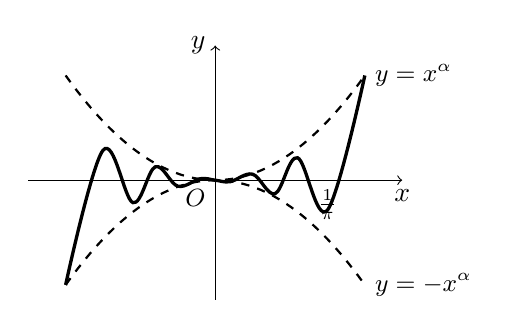
\begin{tikzpicture}[scale=0.95]
  \draw[->] (-2.5,0) -- (2.5,0) node[below] {$x$};
  \draw[->] (0,-1.6) -- (0,1.8) node[left] {$y$};
  \node[below left] at (0,0) {\small $O$};
  
  \draw[dashed, thick, domain=-2:2, samples=50] plot (\x, {0.35*\x*\x}) node[right] {\small $y=x^\alpha$};
  \draw[dashed, thick, domain=-2:2, samples=50] plot (\x, {-0.35*\x*\x}) node[right] {\small $y=-x^\alpha$};
  
  \draw[very thick] plot [smooth, tension=0.6] coordinates {
    (-2.0, -1.4) (-1.5, 0.4) (-1.1, -0.3) (-0.8, 0.18) (-0.5, -0.08) (-0.2, 0.02)
    (0,0)
    (0.2, -0.02) (0.5, 0.08) (0.8, -0.18) (1.1, 0.3) (1.5, -0.4) (2.0, 1.4)
  };
  \node[below] at (1.5,0) {\small $\frac{1}{\pi}$};
\end{tikzpicture}
\caption{}\label{fig:2.1.16}
\end{figure}

\begin{example}\label{ex:2.1.11}
设 $\lim\limits_{x\to x_0}f(x)=0, |g(x)|\leqslant M$, 则 $\lim\limits_{x\to x_0}f(x)g(x)=0$.
\end{example}

\begin{proof}
$\forall\varepsilon>0$, 因 $\lim\limits_{x\to x_0}f(x)=0$, 故 $\exists\delta>0$, 当 $0<|x-x_0|<\delta$ 时, 有 $|f(x)-0|<\frac{\varepsilon}{M+1}$. 于是,
\[
|f(x)g(x)-0|=|f(x)|\cdot|g(x)|\leqslant M|f(x)-0|<M\cdot\frac{\varepsilon}{M+1}<\varepsilon,
\]
这就证明了 $\lim\limits_{x\to x_{0}}f(x)g(x)=0$.
\end{proof}

\begin{example}\label{ex:2.1.12}
设
\[
f(x)=\begin{cases}
1, & x<0, \\
x\sin\frac{1}{x}, & x>0.
\end{cases}
\]
证明: $\lim\limits_{x\to0}f(x)$ 不存在.
\end{example}

\begin{proof}
因为
\begin{align*}
f(0+0) &= f(0^{+})=\lim_{x\to0^{+}}x\sin\frac{1}{x}=0, \\
f(0-0) &= f(0^{-})=\lim_{x\to0^{-}}f(x)=\lim_{x\to0^{-}}1=1,
\end{align*}
$f(0^{+})\neq f(0^{-})$, 所以根据定理~\ref{thm:2.1.1} 知, $\lim\limits_{x\to0}f(x)$ 不存在.
\end{proof}

\begin{example}\label{ex:2.1.13}
证明: 符号函数 $\operatorname{sgn} x$ 在 $x=0$ 处无极限.
\end{example}

\begin{proof}
因为
\[
\operatorname{sgn}(0^{+})=\lim_{x\to0^{+}}\operatorname{sgn} x=\lim_{x\to0^{+}}1=1\neq-1=\lim_{x\to0^{-}}(-1)=\lim_{x\to0^{-}}\operatorname{sgn} x=\operatorname{sgn}(0^{-}),
\]
所以根据定理~\ref{thm:2.1.1} 知, $\operatorname{sgn} x$ 在 $x=0$ 处无极限.
\end{proof}

\begin{example}\label{ex:2.1.14}
证明 $\lim\limits_{x\to0}\sin\frac{1}{x}$ 不存在.
\end{example}

\begin{proof}
取数列 $x_{n}^{\prime}=\frac{1}{2n\pi}\to0\ (n\to+\infty)$, $x_{n}^{\prime\prime}=\frac{1}{2n\pi+\frac{\pi}{2}}\to0\ (n\to+\infty)$. 显然,
\begin{align*}
\lim_{n\to+\infty}\sin\frac{1}{x_{n}^{\prime}} &= \lim_{n\to+\infty}\sin 2n\pi = 0, \\
\lim_{n\to+\infty}\sin\frac{1}{x_{n}^{\prime\prime}} &= \lim_{n\to+\infty}\sin\left(2n\pi+\frac{\pi}{2}\right) = 1,
\end{align*}
$\lim\limits_{n\to+\infty}\sin\frac{1}{x_{n}^{\prime}}\neq\lim\limits_{n\to+\infty}\sin\frac{1}{x_{n}^{\prime\prime}}$. 所以根据定理~\ref{thm:2.1.3} 知, $\lim\limits_{x\to0}\sin\frac{1}{x}$ 不存在(如图~\ref{fig:2.1.17} 所示).
\end{proof}

\begin{figure}[htbp]
\centering
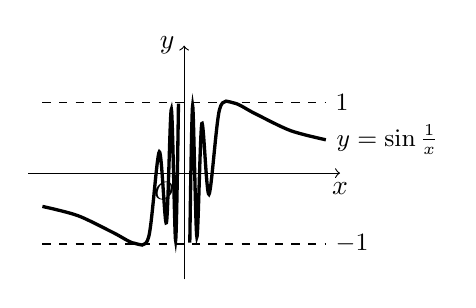
\begin{tikzpicture}[scale=0.9]
  \draw[->] (-2.2,0) -- (2.2,0) node[below] {$x$};
  \draw[->] (0,-1.5) -- (0,1.8) node[left] {$y$};
  \node[below left] at (0,0) {\small $O$};
  
  \draw[dashed] (-2,1) -- (2,1) node[right] {\small $1$};
  \draw[dashed] (-2,-1) -- (2,-1) node[right] {\small $-1$};
  
  \draw[very thick] plot [smooth, tension=0.5] coordinates {
    (-2.0,-0.47) (-1.5,-0.6) (-1.0,-0.84) (-0.7,-0.99) (-0.5,-0.9)
    (-0.35, 0.3) (-0.25, -0.7) (-0.18, 0.9) (-0.12, -0.95) (-0.08, 0.98)
  };
  \draw[very thick] plot [smooth, tension=0.5] coordinates {
    (0.08, -0.98) (0.12, 0.95) (0.18, -0.9) (0.25, 0.7) (0.35, -0.3)
    (0.5, 0.9) (0.7, 0.99) (1.0, 0.84) (1.5, 0.6) (2.0, 0.47)
  } node[right, font=\small] {$y=\sin\frac{1}{x}$};
\end{tikzpicture}
\caption{}\label{fig:2.1.17}
\end{figure}

\begin{example}\label{ex:2.1.15}
证明 Dirichlet 函数
\[
D(x)=\begin{cases}
1, & x\in\mathbb{Q}, \\
0, & x\in\mathbb{R}\setminus\mathbb{Q}
\end{cases}
\]
在任何点处无极限.
\end{example}

\begin{proof}
\textit{证法 1}\quad $\forall x_0 \in \mathbb{R}$, 取 $x'_n \in \mathbb{Q}, x'_n \neq x_0, x'_n \to x_0\ (n \to +\infty)$; 再取 $x''_n \in \mathbb{R} \setminus \mathbb{Q}, x''_n \neq x_0, x''_n \to x_0\ (n \to +\infty)$, 则
\[
\lim_{n\to+\infty}D(x_{n}^{\prime})=\lim_{n\to+\infty}1=1,\quad \lim_{n\to+\infty}D(x_{n}^{\prime \prime})=\lim_{n\to+\infty}0=0.
\]
因为 $\lim\limits_{n\to+\infty}D(x_{n}^{\prime})\neq\lim\limits_{n\to+\infty}D(x_{n}^{\prime\prime})$, 所以根据定理~\ref{thm:2.1.3} 知, $\lim\limits_{x\to x_{0}}D(x)$ 不存在.

\textit{证法 2}\quad (反证)反设在点 $x_{0} \in \mathbb{R}$, $\lim\limits_{x \to x_{0}} D(x) = a$, 则 $0$ 与 $1$ 中至少有一个不为 $a$. 不妨设 $a \neq 1$, 则存在 $a$ 的开邻域 $U(a) \not\ni 1$. 于是, $\exists \delta > 0$, 当 $0 < |x - x_{0}| < \delta$ 时, $D(x) \in U(a)$, 当然 $D(x) \neq 1$. 但因 $\mathbb{Q}$ 在 $\mathbb{R}$ 中是稠密的, 必有 $x' \in \mathbb{Q}$, s.t. $0 < |x' - x_{0}| < \delta$, 所以 $1=D(x^{\prime})\in U(a)$, 这与 $1 \notin U(a)$ 相矛盾.
\end{proof}

\begin{example}\label{ex:2.1.16}
证明:
\[
\lim_{x\to+\infty}a^x=\begin{cases}
+\infty, & a>1, \\
1, & a=1, \\
0, & 0<a<1.
\end{cases}
\]
\end{example}

\begin{proof}
当 $a>1$ 时, $\forall A>0$, 取 $\Delta>\log_{a}A$. 当 $x>\Delta$ 时, 有
\[
a^{x}>a^{\Delta}>A,
\]
所以 $\lim\limits_{x\to+\infty}a^{x}=+\infty$.

当 $0 < a < 1$ 时, $\forall \varepsilon > 0$, 取 $\Delta > \log_{a}\varepsilon$. 当 $x > \Delta$ 时, 有
\[
|a^{x}-0|=a^{x}<a^{\Delta}<\varepsilon,
\]
所以 $\lim\limits_{x\to+\infty}a^{x}=0$.

当 $a=1$ 时, $\lim\limits_{x\to+\infty}a^{x}=\lim\limits_{x\to+\infty}1^{x}=\lim\limits_{x\to+\infty}1=1$.
\end{proof}

\begin{example}\label{ex:2.1.17}
证明:
\begin{enumerate}[label=(\arabic*)]
  \item $\lim\limits_{x\to 0}a^{x}=1\ (a>0)$;
  \item $\lim\limits_{x \to 1} \log_a x = 0\ (a > 0, a \neq 1)$.
\end{enumerate}
\end{example}

\begin{proof}
(1) 设 $a=1$, 显然 $\lim\limits_{x\to0}a^{x}=\lim\limits_{x\to0}1^{x}=1$.

设 $a>1$. $\forall\varepsilon\in(0,1)$, 取 $\delta=\min\{|\log_{a}(1-\varepsilon)|,|\log_{a}(1+\varepsilon)|\}$, 当 $0<|x-0|=|x|<\delta$ 时, 有
\[
\log_{a}(1-\varepsilon)<x<\log_{a}(1+\varepsilon)\implies 1-\varepsilon<a^{x}<1+\varepsilon\implies |a^{x}-1|<\varepsilon,
\]
所以 $\lim\limits_{x\to0} a^x = 1$.

设 $0 < a < 1$. $\forall \varepsilon \in (0,1)$, 取 $\delta = \min\{|\log_{a}(1-\varepsilon)|, |\log_{a}(1+\varepsilon)|\}$, 当 $0 < |x| < \delta$ 时, 有
\[
\log_{a}(1+\varepsilon)<x<\log_{a}(1-\varepsilon)\implies 1-\varepsilon<a^{x}<1+\varepsilon\implies |a^{x}-1|<\varepsilon,
\]
所以 $\lim\limits_{x\to0}a^{x}=1$.

(2) 不失一般性, 设 $a > 1$. $\forall \varepsilon > 0$, 必存在 $\varepsilon_{1} > 0$, 使得 $a^{-\varepsilon} < 1 - \varepsilon_{1} < 1 + \varepsilon_{1} < a^{\varepsilon}$. 当 $a^{-\varepsilon}<1-\varepsilon_{1}<x<1+\varepsilon_{1}<a^{\varepsilon}$ 时, 有
\[
-\varepsilon<\log_{a}x<\varepsilon\implies |\log_{a}x-0|<\varepsilon,
\]
故 $\lim\limits_{x\to1}\log_{a}x=0$.
\end{proof}

\begin{lemma}\label{lem:2.1.1}
证明:
\begin{enumerate}[label=(\arabic*)]
  \item $\sin x < x < \tan x,\ 0 < x < \frac{\pi}{2}$;
  \item $\sin x < x,\ \forall x \in (0, +\infty)$;
  \item $|\sin x|\leqslant|x|,\ \forall x\in\mathbb{R}$.
\end{enumerate}
\end{lemma}

\begin{proof}
(1) 图~\ref{fig:2.1.18} 所示是一单位圆, 用 $S_{\triangle OCD}, S_{\text{扇形}OAD}, S_{\triangle OAB}$ 分别表示 $\triangle OCD$, 扇形 $OAD$ 和 $\triangle OAB$ 的面积. 显然,
\[
S_{\triangle OCD}<S_{\text{扇形}OAD}<S_{\triangle OAB},
\]
从而 $\frac{1}{2}\sin x\cos x < \frac{1}{2}x < \frac{1}{2}\tan x$, 于是 $\sin x<x<\tan x\ (0<x<\frac{\pi}{2})$.

\begin{figure}[htbp]
\centering
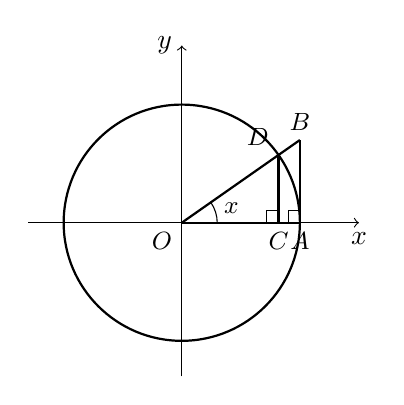
\begin{tikzpicture}[scale=1.5]
  \draw[->] (-1.3,0) -- (1.5,0) node[below] {$x$};
  \draw[->] (0,-1.3) -- (0,1.5) node[left] {$y$};
  \node[below left] at (0,0) {\small $O$};
  
  \draw[thick] (0,0) circle (1cm);
  
  \coordinate (O) at (0,0);
  \coordinate (A) at (1,0);
  \coordinate (D) at ({cos(35)}, {sin(35)});
  \coordinate (C) at ({cos(35)}, 0);
  \coordinate (B) at (1, {tan(35)});
  
  \draw[thick] (O) -- (B);
  \draw[thick] (A) -- (B);
  \draw[thick] (C) -- (D);
  \draw[thick] (O) -- (A);
  
  \node[below] at (A) {\small $A$};
  \node[above] at (B) {\small $B$};
  \node[above left] at (D) {\small $D$};
  \node[below] at (C) {\small $C$};
  
  \draw (0.3,0) arc (0:35:0.3);
  \node at (0.42,0.12) {\small $x$};
  
  \draw (0.9,0) -- (0.9,0.1) -- (1,0.1);
  \draw ({cos(35)},0.1) -- ({cos(35)-0.1},0.1) -- ({cos(35)-0.1},0);
\end{tikzpicture}
\caption{}\label{fig:2.1.18}
\end{figure}

(2) 当 $x \geqslant \frac{\pi}{2}$ 时, $x \geqslant \frac{\pi}{2} > 1 \geqslant \sin x$, 因此 $\sin x<x,\ \forall x\in(0,+\infty)$.

当 $x<0$ 时, $|\sin x|=|\sin(-x)|<-x=|x|$. 结合 $x=0$ 处等号成立, 故 $|\sin x|\leqslant|x|,\ \forall x\in\mathbb{R}$.
\end{proof}

\begin{example}\label{ex:2.1.18}
证明:
\begin{enumerate}[label=(\arabic*)]
  \item $\lim\limits_{x \to x_0} \sin x = \sin x_0$;
  \item $\lim\limits_{x \to x_0} \cos x = \cos x_0\ (x_0 \in \mathbb{R})$.
\end{enumerate}
\end{example}

\begin{proof}
(1) $\forall\varepsilon>0$, 取 $\delta=\varepsilon$, 当 $|x-x_{0}|<\delta$ 时, 由和差化积公式与引理~\ref{lem:2.1.1} 有
\[
|\sin x-\sin x_{0}|=2\left|\cos\frac{x+x_{0}}{2}\right|\left|\sin\frac{x-x_{0}}{2}\right|\leqslant2\left|\frac{x-x_{0}}{2}\right|=|x-x_{0}|<\delta=\varepsilon,
\]
所以 $\lim\limits_{x\to x_0}\sin x=\sin x_0$.

(2) 同理, $\forall\varepsilon>0$, 取 $\delta=\varepsilon$, 当 $|x-x_{0}|<\delta$ 时, 有
\[
|\cos x-\cos x_{0}|=2\left|\sin\frac{x+x_{0}}{2}\right|\left|\sin\frac{x-x_{0}}{2}\right|\leqslant2\left|\frac{x-x_{0}}{2}\right|<\delta=\varepsilon,
\]
所以 $\lim\limits_{x\to x_0}\cos x=\cos x_0$. 或由 $\lim\limits_{x\to x_0}\cos x=\lim\limits_{x\to x_0}\sin\left(\frac{\pi}{2}-x\right)=\sin\left(\frac{\pi}{2}-x_0\right)=\cos x_0$.
\end{proof}

\begin{example}\label{ex:2.1.19}
证明: $\lim\limits_{x\to x_0}\sqrt{x}=\sqrt{x_0}\ (x_0\geqslant0)$.
\end{example}

\begin{proof}
当 $x_{0}=0$ 时, $\forall\varepsilon>0$, 取 $\delta=\varepsilon^{2}$, 当 $0<x<\delta$ 时, 有
\[
|\sqrt{x}-\sqrt{0}|=\sqrt{x}<\sqrt{\delta}=\varepsilon,
\]
故 $\lim\limits_{x\to0^{+}}\sqrt{x}=0$.

当 $x_{0}>0$ 时, 取 $\delta=\min\{x_{0},\sqrt{x_{0}}\varepsilon\}$, 当 $|x-x_{0}|<\delta$ 时, 有
\[
|\sqrt{x}-\sqrt{x_{0}}|=\frac{|x-x_{0}|}{\sqrt{x}+\sqrt{x_{0}}}\leqslant\frac{|x-x_{0}|}{\sqrt{x_{0}}}<\frac{\delta}{\sqrt{x_{0}}}\leqslant\varepsilon,
\]
所以 $\lim\limits_{x\to x_0}\sqrt{x}=\sqrt{x_0}$.
\end{proof}

\begin{example}\label{ex:2.1.20}
证明: $\lim\limits_{x\to\infty}\sqrt{\frac{x^{2}+1}{x^{2}-1}}=1$.
\end{example}

\begin{proof}
\textit{证法 1}\quad $\forall\varepsilon>0$, 取 $\Delta>\max\left\{\sqrt{2},\frac{2}{\varepsilon}\right\}$, 当 $|x|>\Delta$ 时, 有
\begin{align*}
\left|\sqrt{\frac{x^2+1}{x^2-1}}-1\right| &= \left|\frac{\sqrt{x^2+1}-\sqrt{x^2-1}}{\sqrt{x^2-1}}\right|=\frac{2}{\sqrt{x^2-1}(\sqrt{x^2+1}+\sqrt{x^2-1})} \\
&< \frac{2}{x^2-1} \leqslant \frac{2}{\frac{1}{2}x^2} = \frac{4}{x^2} < \varepsilon,
\end{align*}
或放大为 $\frac{2}{|x|} < \frac{2}{\Delta} < \varepsilon$. 所以 $\lim\limits_{x\to\infty}\sqrt{\frac{x^{2}+1}{x^{2}-1}}=1$.

\textit{证法 2}\quad 变形为
\[
\lim_{x\to\infty}\sqrt{\frac{x^{2}+1}{x^{2}-1}}=\lim_{x\to\infty}\sqrt{\frac{1+\frac{1}{x^{2}}}{1-\frac{1}{x^{2}}}}=\sqrt{\frac{1+0}{1-0}}=1.
\]
\end{proof}

\begin{exblock}{练习题 2.1}
  \item 在定义~\ref{def:2.1.3} 中就 24 种情形给出函数极限的定义, 并配出相应的图形.
  \item 按函数极限的定义证明:
  \begin{enumerate}[label=(\arabic*)]
    \item $\lim\limits_{x \to +\infty} \frac{6x + 5}{x} = 6$;
    \item $\lim\limits_{x \to 2} (x^2 - 6x + 10) = 2$;
    \item $\lim\limits_{x \to +\infty} \frac{x^2 - 5}{x^2 - 1} = 1$;
    \item $\lim\limits_{x \to 2^-} \sqrt{4 - x^2} = 0$;
    \item $\lim\limits_{x \to 1} \frac{x^4 - 1}{x - 1} = 4$;
    \item $\lim\limits_{x \to 3} \frac{x - 3}{x^2 - 9} = \frac{1}{6}$;
    \item $\lim\limits_{x\to1^{+}}\frac{x-1}{\sqrt{x^{2}-1}}=0$;
    \item $\lim\limits_{x \to +\infty} (\sqrt{x+1} - \sqrt{x-1}) = 0$;
    \item $\lim\limits_{x \to \infty} \sqrt{\frac{x^2 + 2}{x^2 - 2}} = 1$.
  \end{enumerate}
  \item 设 $\lim\limits_{x \to x_0} f(x) = a$. 用 $\varepsilon - \delta$ 法证明:
  \begin{enumerate}[label=(\arabic*)]
    \item $\lim\limits_{x \to x_0} f^2(x) = a^2$;
    \item $\lim\limits_{x \to x_0} \sqrt{f(x)} = \sqrt{a}\ (a > 0)$;
    \item $\lim\limits_{x \to x_0} \sqrt[3]{f(x)} = \sqrt[3]{a}$.
  \end{enumerate}
  \item 设 $\lim\limits_{x \to x_0} f(x) = a$. 证明: $\lim\limits_{x \to x_0} |f(x)| = |a|$. 举例说明反之不成立. 问: 当且仅当 $a$ 为何值时反之也成立?
  \item 讨论下列函数在点 $0$ 处的极限或左、右极限:
  \begin{enumerate}[label=(\arabic*)]
    \item $f(x)=\frac{|x|}{x}$;
    \item $f(x)=[x]$;
    \item $f(x)=\begin{cases} 2^{x}, & x>0, \\ 0, & x=0, \\ 1+x^{2}, & x<0. \end{cases}$
  \end{enumerate}
  \item 设 $f(x)=\begin{cases} x^{2}, & x\geqslant2, \\ -ax, & x<2. \end{cases}$
  \begin{enumerate}[label=(\arabic*)]
    \item 求 $f(2^{+}), f(2^{-})$;
    \item 若 $\lim\limits_{x\to2}f(x)$ 存在, $a$ 应为何值.
  \end{enumerate}
  \item 设 $f(x_{0}^{-}) < f(x_{0}^{+})$. 证明: $\exists\delta > 0$, s.t. 当 $x_{0} - \delta < x < x_{0} < y < x_{0} + \delta$ 时, 有 $f(x) < f(y)$.
  \item 设 $f$ 在 $(-\infty, x_0)$ 内单调增, 且有一数列 $\{x_n\}$, 适合 $x_n < x_0\ (n \in \mathbb{N})$, $x_n \to x_0^-$ 及 $\lim\limits_{n \to +\infty} f(x_n) = a$. 证明: $f(x_0^-) = a = \sup\limits_{x \in U_-(x_0)} f(x)$.
  \item 用肯定的语气表述 $\lim\limits_{x \to x_{0}} f(x) \neq a$.
  \item $\forall n \in \mathbb{N}, A_n \subset [0,1]$ 为有限集, 且 $A_i \cap A_j = \varnothing\ (i \neq j), i, j \in \mathbb{N}$. 定义函数
  \[
  f(x)=\begin{cases}
  \frac{1}{n}, & x\in A_{n}, \\
  0, & x\in[0,1]\setminus\bigcup\limits_{n=1}^{\infty}A_{n}.
\end{cases}
\]
  对 $\forall x_0\in[0,1]$, 求 $\lim\limits_{x\to x_0}f(x)$.
  \item 叙述函数极限 $\lim\limits_{x \to +\infty} f(x)$ 的归结原则, 并应用它证明: $\lim\limits_{x \to +\infty} \sin x$ 与 $\lim\limits_{x \to +\infty} \cos x$ 都不存在.
  \item \begin{enumerate}[label=(\arabic*)]
    \item 叙述极限 $\lim\limits_{x \to +\infty} f(x)$ 的 Cauchy 准则;
    \item 根据 Cauchy 准则叙述 $\lim\limits_{x \to +\infty} f(x)$ 不存在的充要条件, 并应用它证明 $\lim\limits_{x \to +\infty} \sin x$ 与 $\lim\limits_{x \to +\infty} \cos x$ 不存在.
  \item 设 $f$ 为周期函数, 且 $\lim\limits_{x\to+\infty}f(x)=0$. 证明: $f(x)\equiv0$.
  \item 设 $f$ 在 $U^{\circ}(x_{0})$ 内有定义. 证明: 若对 $\forall \{x_{n}\} \subseteq U^{\circ}(x_{0})$ 且 $\lim\limits_{n\to+\infty}x_{n}=x_{0}$, 极限 $\lim\limits_{n\to+\infty}f(x_{n})$ 都存在(实数, 或 $+\infty$, 或 $-\infty$), 则所有这些极限都相等.
  \item 设 $f$ 为定义在 $[a, +\infty)$ 上的增(减)函数. 证明: $\lim\limits_{x \to +\infty} f(x)$ 存在有限的充要条件是 $f$ 在 $[a, +\infty)$ 上有上(下)界.
  \item 设 $f$ 为 $U^{\circ}(x_{0})$ 上的单调增函数, 证明: $f(x_{0}^{-})$ 与 $f(x_{0}^{+})$ 均存在且有限, 且
  \[
  f(x_{0}^{-})=\sup_{x\in U_{-}^{\circ}(x_{0})}f(x),\quad f(x_{0}^{+})=\inf_{x\in U_{+}^{\circ}(x_{0})}f(x).
\]
\end{enumerate}
\end{exblock}

\begin{exblock}{思考题 2.1}
  \item \begin{enumerate}[label=(\arabic*)]
    \item 设函数 $f$ 在 $(0, +\infty)$ 上满足方程 $f(2x) = f(x)$, 且 $\lim\limits_{x \to +\infty} f(x) = a$. 证明: $f(x) \equiv a$.
    \item 设函数 $f$ 在 $(0, +\infty)$ 上满足方程 $f(x^{2}) = f(x)$, 且
    \[
    \lim_{x\to0^{+}}f(x)=\lim_{x\to+\infty}f(x)=f(1).
\]
    证明: $f(x) \equiv f(1), x \in (0, +\infty)$.
  \item 设函数 $f\colon (a, +\infty) \to \mathbb{R}$ 在任意有限区间 $(a, b)$ 内有界, 且
  \[
  \lim_{x\to+\infty}\left[f(x+1)-f(x)\right]=A.
\]
  证明: $\lim\limits_{x\to+\infty}\frac{f(x)}{x}=A$.
  \item 设 $a > 1, b > 1$ 为两个常数, 函数 $f\colon \mathbb{R} \to \mathbb{R}$ 在 $x = 0$ 的近旁有界, 且 $\forall x \in \mathbb{R}$, 有 $f(ax) = bf(x)$. 证明: $\lim\limits_{x \to 0} f(x) = f(0)$.
\end{enumerate}
\end{exblock}

% ====================================================================
%  徐森林、薛春华《数学分析》（第一册）
%  \S2.2  函数极限的性质
%  源：原书印刷页 99-115（PDF 物理页 105-121）
%  约定：全西文半角标点；单一落盘出口 write_tex；display 数学环境无空行；
%        原生 TikZ 矢量制图；定理/定义/例/练习题/思考题全量高保真收录
% ====================================================================
\section{函数极限的性质}\label{sec:2.2}

与数列极限一样, 函数极限有惟一性定理、局部有界性、局部保号性、保不等式性、夹逼定理、极限的四则运算法则. 此外, 还有复合函数求极限的定理. 这些性质对求函数的极限又有很大的作用.

\begin{theorem}[极限的惟一性]\label{thm:2.2.1}
如果函数 $f(x)$ 在 $x_{0}(x_{0}^{\pm},\allowbreak \pm\infty, \infty)$ 处有极限 $a$ (实数、 $+\infty,\allowbreak -\infty$), 则极限惟一.
\end{theorem}

\begin{proof}
\textit{证法 1}\quad 设 $a, b \in \mathbb{R}$ 都为 $f(x)$ 当 $x \to x_0$ 时的极限, 则 $\forall \varepsilon > 0$,
\[
\exists\,\delta_{1}>0,\text{ s.t. 当 } 0<|x-x_{0}|<\delta_{1} \text{ 时, 有 } |f(x)-a|<\frac{\varepsilon}{2},
\]
\[
\exists\,\delta_{2}>0,\text{ s.t. 当 } 0<|x-x_{0}|<\delta_{2} \text{ 时, 有 } |f(x)-b|<\frac{\varepsilon}{2}.
\]
于是, 当 $0<|x-x_0|<\delta=\min\{\delta_1,\delta_2\}$ 时, 有
\begin{align*}
0\leqslant |a-b| &= |(f(x)-a)-(f(x)-b)| \\
&\leqslant |f(x)-a|+|f(x)-b| < \frac{\varepsilon}{2}+\frac{\varepsilon}{2}=\varepsilon.
\end{align*}
令 $\varepsilon \to 0^{+}$, 得到 $0 \leqslant |a - b| \leqslant 0$, 故 $|a - b| = 0$, 即 $a = b$.

此证法不能推广到其他情形.

\textit{证法 2 (反证法)}\quad 反设 $f(x)$ 在 $x_{0}$ 处有两个不同的极限 $a, b$ ($a \neq b$). 取 $a$ 的开邻域 $V(a)$, $b$ 的开邻域 $V(b)$, 使得 $V(a) \cap V(b) = \varnothing$. 于是, 存在 $x_{0}$ 的去心开邻域 $U_{1}^{\circ}(x_{0})$, 当 $x \in U_{1}^{\circ}(x_{0})$ 时, $f(x) \in V(a)$; 存在 $x_{0}$ 的去心开邻域 $U_{2}^{\circ}(x_{0})$, 当 $x \in U_{2}^{\circ}(x_{0})$ 时, 有 $f(x) \in V(b)$. 因此, 当 $x \in U_{1}^{\circ}(x_{0}) \cap U_{2}^{\circ}(x_{0})$ 时, 有
\[
f(x)\in V(a)\cap V(b)=\varnothing,
\]
矛盾.
\end{proof}

\begin{definition}\label{def:2.2.1}
设 $f: X \to \mathbb{R}$ 为实值函数. 如果存在 $M \geqslant 0$, s.t. $|f(x)| \leqslant M$, $\forall x \in X$, 则称 $f(x)$ 在 $X$ 上有界; 如果存在 $B \in \mathbb{R}$, s.t. $f(x) \leqslant B$, $\forall x \in X$, 则称 $f(x)$ 在 $X$ 上有上界; 如果存在 $A \in \mathbb{R}$, s.t. $f(x) \geqslant A$, $\forall x \in X$, 则称 $f(x)$ 在 $X$ 上有下界 $A$. 显然,
\[
f(x) \text{ 在 } X \text{ 上有界} \iff f(x) \text{ 在 } X \text{ 上既有上界又有下界}.
\]
如: $|\sin x|\leqslant 1$, $\forall x\in\mathbb{R}$, 故 $\sin x$ 在 $\mathbb{R}$ 上有界; $e^{x}>0$, 故有下界 $0$, 但它无上界.
\end{definition}

\begin{theorem}[局部有界性]\label{thm:2.2.2}
如果 $f(x)$ 在 $x_{0}(x_{0}^{\pm}, \pm\infty, \infty)$ 处有有限极限, 则 $f(x)$ 在 $x_{0}(x_{0}^{\pm},\allowbreak \pm\infty,\allowbreak \infty)$ 的某去心开邻域 (附近) 中有界.
\end{theorem}

\begin{proof}
设 $\lim\limits_{x \to x_0} f(x) = a \in \mathbb{R}$, 取 $\varepsilon_0 = 1$, 则有 $x_0$ 的去心开邻域 $U^\circ(x_0)$, 当 $x \in U^\circ(x_0)$ 时, 有
\[
|f(x)-a|<\varepsilon_{0}=1,
\]
所以
\[
|f(x)|=|(f(x)-a)+a|\leqslant|f(x)-a|+|a|<1+|a|.
\]
这就证明了 $f(x)$ 在 $x_{0}$ 的去心开邻域 $U^{\circ}(x_{0})$ 中有界.
\end{proof}

\begin{theorem}[局部保号性]\label{thm:2.2.3}
设 $f(x)$ 在 $x_{0}(x_{0}^{\pm}, \pm\infty, \infty)$ 处有有限极限 $a > 0$ (或 $<0$), 则 $\forall r \in (0, a)$ (或 $r \in (a, 0)$), 存在 $x_{0}$ 的去心开邻域 $U^{\circ}(x_{0})$, s.t. $\forall x \in U^{\circ}(x_{0})$ 有
\[
f(x)>r>0 \quad (\text{或 } f(x)<r<0).
\]
\end{theorem}

\begin{proof}
设 $a > 0$, $\forall r \in (0, a)$, 令 $\varepsilon = a - r > 0$. 由 $\lim\limits_{x \to x_0} f(x) = a$, 故存在 $x_0$ 的去心开邻域 $U^\circ(x_0)$, 当 $x \in U^\circ(x_0)$ 时, 有
\[
f(x)>a-\varepsilon=a-(a-r)=r>0.
\]
$a<0$ 的情形可类似证明, 或用 $-f(x)$ 代替 $f(x)$.
\end{proof}

\begin{theorem}[保不等式性]\label{thm:2.2.4}
设 $f(x), g(x)$ 在 $x_{0}(x_{0}^{\pm}, \pm\infty, \infty)$ 均有极限 (实数, $+\infty, -\infty$), 且在 $x_{0}$ 的去心开邻域 $U^{\circ}(x_{0})$ 内有 $f(x) \leqslant g(x)$, 则
\[
\lim_{x\to x_{0}}f(x)\leqslant\lim_{x\to x_{0}}g(x).
\]
\end{theorem}

\begin{proof}
\textit{证法 1}\quad 设 $\lim\limits_{x \to x_0} f(x) = a \in \mathbb{R}$, $\lim\limits_{x \to x_0} g(x) = b \in \mathbb{R}$, 则 $\forall \varepsilon > 0$, 存在 $x_0$ 的去心开邻域 $U_1^\circ(x_0) \subset U^\circ(x_0)$, 当 $x \in U_1^\circ(x_0)$ 时, 有 $a - \varepsilon < f(x)$; 存在 $x_0$ 的去心开邻域 $U_2^\circ(x_0) \subset U^\circ(x_0)$, 当 $x \in U_2^\circ(x_0)$ 时有 $g(x) < b + \varepsilon$. 因此当 $x \in U_1^\circ(x_0) \cap U_2^\circ(x_0)$ 时, 有
\[
a-\varepsilon<f(x)\leqslant g(x)<b+\varepsilon,
\]
所以 $a < b + 2\varepsilon$. 令 $\varepsilon \to 0^{+}$, 得到 $a \leqslant b$.

其他情形为 $\lim\limits_{x \to x_0} f(x) = -\infty \leqslant \lim\limits_{x \to x_0} g(x)$; $\lim\limits_{x \to x_0} f(x) = +\infty = \lim\limits_{x \to x_0} g(x)$; $\lim\limits_{x \to x_0} f(x) = -\infty = \lim\limits_{x \to x_0} g(x)$; 以及 $\lim\limits_{x \to x_0} f(x) \leqslant +\infty = \lim\limits_{x \to x_0} g(x)$.

\textit{证法 2 (反证法)}\quad 反设 $\lim\limits_{x\to x_{0}}f(x)=a>b=\lim\limits_{x\to x_{0}}g(x)$, 则存在 $a$ 的开邻域 $V(a)$ 以及 $b$ 的开邻域 $V(b)$, s.t. $V(a)\cap V(b)=\varnothing$. 于是, 存在 $x_{0}$ 的去心开邻域 $U_{1}^{\circ}(x_{0})\subset U^{\circ}(x_{0})$, 当 $x\in U_{1}^{\circ}(x_{0})$ 时, 有 $f(x)\in V(a)$; 存在 $x_{0}$ 的去心开邻域 $U_{2}^{\circ}(x_{0})\subset U^{\circ}(x_{0})$, 当 $x\in U_{2}^{\circ}(x_{0})$ 时, 有 $g(x)\in V(b)$. 则当 $x\in U_{1}^{\circ}(x_{0})\cap U_{2}^{\circ}(x_{0})=U_{3}^{\circ}(x_{0})$, 有
\[
g(x)<f(x).
\]
这与已知 $f(x) \leqslant g(x)$ 相矛盾.
\end{proof}

\begin{theorem}[夹逼定理]\label{thm:2.2.5}
设 $f(x), g(x)$ 在 $x_{0}(x_{0}^{\pm}, \pm\infty, \infty)$ 有极限 $a$ (实数, $+\infty, -\infty$), 且在 $x_{0}$ 某去心开邻域 $U^{\circ}(x_{0})$ 内有
\[
f(x)\leqslant h(x)\leqslant g(x),
\]
那么
\[
\lim_{x\to x_{0}}h(x)=a.
\]
\end{theorem}

\begin{proof}
\textit{证法 1}\quad 当 $x_{0}\in\mathbb{R}, a\in\mathbb{R}, U^{\circ}(x_{0})=U^{\circ}(x_{0},\delta_{0})$ 时, $\forall\varepsilon>0$, 由 $\lim\limits_{x\to x_{0}}f(x)=\lim\limits_{x\to x_{0}}g(x)=a$, 可知:
\begin{align*}
\exists\,\delta_1 \in (0, \delta_0),&\text{ 当 } 0 < |x - x_0| < \delta_1 \text{ 时, 有 } a - \varepsilon < f(x); \\
\exists\,\delta_{2}\in(0,\delta_{0}),&\text{ 当 } 0<|x-x_{0}|<\delta_{2} \text{ 时, 有 } g(x)<a+\varepsilon.
\end{align*}
于是, 当 $0<|x-x_0|<\delta=\min\{\delta_1,\delta_2\}$ 时, 有
\[
a-\varepsilon<f(x)\leqslant h(x)\leqslant g(x)<a+\varepsilon,
\]
所以 $\lim\limits_{x\to x_0}h(x)=a$.

其他情形类似证明.

\textit{证法 2 (统一描述)}\quad 对 $a$ 的任何开邻域 $V(a)$, 因为 $\lim\limits_{x\to x_0}f(x)=\lim\limits_{x\to x_0}g(x)=a$, 所以存在 $x_0$ 的去心开邻域 $U_1^\circ(x_0)\subset U^\circ(x_0)$, 当 $x\in U_1^\circ(x_0)$ 时, 有 $f(x)\in V(a)$; 存在 $x_0$ 的去心开邻域 $U_2^\circ(x_0)\subset U^\circ(x_0)$, 当 $x\in U_2^\circ(x_0)$ 时, 有 $g(x)\in V(a)$. 于是, 当 $x\in U_1^\circ(x_0)\cap U_2^\circ(x_0)=U_3^\circ(x_0)$ 时, 由于 $f(x)\leqslant h(x)\leqslant g(x)$, 有
\[
h(x)\in[f(x),g(x)]\subset V(a),
\]
从而 $\lim\limits_{x\to x_{0}}h(x)=a$.
\end{proof}

\begin{remark}\label{rem:2.2.1}
夹逼定理中, 如果 $a=\infty$, 则结论未必成立. 反例: $f(x)=-\frac{1}{(x-x_{0})^{2}}$, $h(x)=0$, $g(x)=\frac{1}{(x-x_{0})^{2}}$.
\end{remark}

\begin{theorem}[极限的四则运算法则]\label{thm:2.2.6}
设 $f(x), g(x)$ 在 $x_{0}(x_{0}^{\pm}, \pm\infty, \infty)$ 处有有限极限, 则 $f \pm g$, $f \cdot g$ 也在 $x_{0}(x_{0}^{\pm}, \pm\infty, \infty)$ 处有有限极限. 又如果 $\lim\limits_{x \to x_{0}} g(x) \neq 0$, 则 $\frac{f}{g}$ 在 $x_{0}(x_{0}^{\pm}, \pm\infty, \infty)$ 处也有有限极限, 且有下列运算公式:
\begin{enumerate}[label=(\arabic*)]
  \item $\lim\limits_{x \to x_0} (f(x) \pm g(x)) = \lim\limits_{x \to x_0} f(x) \pm \lim\limits_{x \to x_0} g(x)$;
  \item $\lim\limits_{x \to x_0} (f(x) \cdot g(x)) = \lim\limits_{x \to x_0} f(x) \cdot \lim\limits_{x \to x_0} g(x)$; 特别地, $\lim\limits_{x \to x_0} c f(x) = c \lim\limits_{x \to x_0} f(x)$;
  \item $\lim\limits_{x \to x_0} \frac{f(x)}{g(x)} = \frac{\lim\limits_{x \to x_0} f(x)}{\lim\limits_{x \to x_0} g(x)} \quad \left(\lim\limits_{x \to x_0} g(x) \neq 0\right)$.
\end{enumerate}
\end{theorem}

\begin{proof}
设 $\lim\limits_{x\to x_0}f(x)=a$, $\lim\limits_{x\to x_0}g(x)=b$.

(1) $\forall \varepsilon > 0$, 存在 $x_0$ 的去心开邻域 $U^\circ(x_0)$, 当 $x \in U^\circ(x_0)$ 时, 有 $|f(x) - a| < \frac{\varepsilon}{2}$, $|g(x) - b| < \frac{\varepsilon}{2}$, 因此
\begin{align*}
|(f(x)\pm g(x))-(a\pm b)| &= |(f(x)-a)\pm(g(x)-b)| \\
&\leqslant |f(x)-a|+|g(x)-b|<\frac{\varepsilon}{2}+\frac{\varepsilon}{2}=\varepsilon,
\end{align*}
于是
\[
\lim_{x\to x_{0}}(f(x)\pm g(x))=a\pm b=\lim_{x\to x_{0}}f(x)\pm\lim_{x\to x_{0}}g(x).
\]

(2) $\forall\varepsilon>0$, 存在 $x_{0}$ 的去心开邻域 $U_{i}^{\circ}(x_{0})\ (i=1,2,3)$, s.t.
\begin{align*}
\text{当 } x \in U_{1}^{\circ}(x_{0}) \text{ 时},&\quad |g(x)| \leqslant M; \\
\text{当 } x \in U_{2}^{\circ}(x_{0}) \text{ 时},&\quad |f(x)-a| < \frac{\varepsilon}{M+|a|+1}; \\
\text{当 } x \in U_3^\circ(x_0) \text{ 时},&\quad |g(x)-b| < \frac{\varepsilon}{M+|a|+1}.
\end{align*}
于是, 当 $x \in U^{\circ}(x_{0}) = U_{1}^{\circ}(x_{0}) \cap U_{2}^{\circ}(x_{0}) \cap U_{3}^{\circ}(x_{0})$ 时, 有
\begin{align*}
|f(x)g(x)-ab| &= |(f(x)-a)g(x)+a(g(x)-b)| \\
&\leqslant |g(x)||f(x)-a|+|a||g(x)-b| \\
&\leqslant M\cdot\frac{\varepsilon}{M+|a|+1}+|a|\frac{\varepsilon}{M+|a|+1} < \varepsilon,
\end{align*}
所以
\[
\lim_{x\to x_{0}}f(x)g(x)=ab=\lim_{x\to x_{0}}f(x)\cdot\lim_{x\to x_{0}}g(x).
\]
特别地, 当 $g(x) \equiv c$ 为常数函数时, 就有 $\lim\limits_{x \to x_0} c f(x) = c \lim\limits_{x \to x_0} f(x)$.

(3) $\forall\varepsilon>0$, 由 $\lim\limits_{x\to x_0}g(x)=b\neq0$ 可知, $\lim\limits_{x\to x_0}|g(x)|=|b|$, 且存在 $x_0$ 的去心开邻域 $U^\circ(x_0)$, 当 $x\in U^\circ(x_0)$ 时, 有 $|g(x)|>\frac{|b|}{2}$, $|g(x)-b|<\frac{b^2}{2}\varepsilon$. 于是
\[
\left|\frac{1}{g(x)}-\frac{1}{b}\right|=\frac{|g(x)-b|}{|b||g(x)|}\leqslant\frac{2}{b^2}\cdot\frac{b^2}{2}\varepsilon=\varepsilon,
\]
所以
\[
\lim_{x\to x_{0}}\frac{1}{g(x)}=\frac{1}{b}.
\]
再根据 (2) 得到
\[
\lim_{x\to x_{0}}\frac{f(x)}{g(x)}=\lim_{x\to x_{0}}\left(f(x)\cdot\frac{1}{g(x)}\right)=a\cdot\frac{1}{b}=\frac{a}{b}=\frac{\lim\limits_{x\to x_{0}}f(x)}{\lim\limits_{x\to x_{0}}g(x)}.
\]
\end{proof}

\begin{remark}\label{rem:2.2.2}
类似定理~\ref{thm:1.2.7}, 读者可给出函数极限的相应定理.
\end{remark}

\begin{theorem}[复合函数的极限]\label{thm:2.2.7}
设函数 $f(u)$ 在 $u_{0}(u_{0}^{\pm}, \pm\infty, \infty)$ 处有极限, 又 $u=\varphi(x)$ 在 $x_{0}(x_{0}^{\pm}, \pm\infty, \infty)$ 处有极限, 且当 $x \to x_{0}, x \neq x_{0}$ 时, $\varphi(x) \to u_{0}, \varphi(x) \neq u_{0}$, 则复合函数 $f\circ\varphi(x) = f(\varphi(x))$ 在 $x_{0}(x_{0}^{\pm}, \pm\infty, \infty)$ 处也有极限, 且
\[
\lim_{x\to x_{0}}f(\varphi(x))=\lim_{u\to u_{0}}f(u).
\]
特别地, 如果 $f(u)$ 在 $u_{0} \in \mathbb{R}$ 处连续, 即 $\lim\limits_{u \to u_0} f(u) = f(u_{0})$, 则
\[
\lim_{x\to x_{0}}f(\varphi(x))=\lim_{u\to u_{0}}f(u)=f(u_{0})=f\left(\lim_{x\to x_{0}}\varphi(x)\right).
\]
这表明 $f$ 与 $\lim$ 可交换, 或极限运算 $\lim$ 可搬到复合函数里.
\end{theorem}

\begin{proof}
设 $x_{0} \in \mathbb{R}$, $u_{0} \in \mathbb{R}$, $\lim\limits_{u \to u_{0}} f(u) = a \in \mathbb{R}$, 则 $\forall \varepsilon > 0$, $\exists\,\delta > 0$, 当 $0 < |u - u_{0}| < \delta$ 时,
\[
|f(u)-a|<\varepsilon.
\]
对同样的 $\delta>0$, 因 $\lim\limits_{x\to x_0}\varphi(x)=u_0,\ \varphi(x)\neq u_0$, 故 $\exists\,\sigma>0$, 当 $0<|x-x_0|<\sigma$ 时,
\[
0<|\varphi(x)-u_{0}|<\delta,
\]
所以
\[
|f(\varphi(x))-a|<\varepsilon,
\]
\[
\lim_{x\to x_{0}}f(\varphi(x))=a=\lim_{u\to u_{0}}f(u).
\]
其他情形类似证明. 请读者用统一描述论证.
\end{proof}

\begin{remark}\label{rem:2.2.3}
定理~\ref{thm:2.2.7} 中, $\varphi(x)\neq u_{0}$ 这一条件不可删去.

反例: 设
\[
f(u)=\begin{cases}
1, & u\neq 0, \\
0, & u=0,
\end{cases}
\]
则 $\lim\limits_{u\to 0}f(u)=1$. 再令 $\varphi(x)=0$, 则 $\lim\limits_{x\to x_0}\varphi(x)=0$. 于是
\[
\lim_{x\to x_{0}}f(\varphi(x))=\lim_{x\to x_{0}}f(0)=\lim_{x\to x_{0}}0=0 \neq 1=\lim_{u\to 0}1=\lim_{u\to 0}f(u).
\]
\end{remark}

\begin{example}\label{ex:2.2.1}
求极限:
\begin{enumerate}[label=(\arabic*)]
  \item $\lim\limits_{x \to \frac{\pi}{4}} (x \cdot \tan x - 1)$;
  \item $\lim\limits_{x\to -1}\left(\frac{1}{x+1}-\frac{3}{x^{3}+1}\right)$.
\end{enumerate}
\end{example}

\begin{solution}
(1) $\lim\limits_{x \to \frac{\pi}{4}} (x \cdot \tan x - 1) = \lim\limits_{x \to \frac{\pi}{4}} \left( x \cdot \frac{\sin x}{\cos x} - 1 \right) = \frac{\pi}{4} \cdot \frac{\sin \frac{\pi}{4}}{\cos \frac{\pi}{4}} - 1 = \frac{\pi}{4} - 1$.

(2) 因为 $\lim\limits_{x\to -1}(x+1)=0$, $\lim\limits_{x\to -1}(x^3+1)=0$, 所以这里不能直接用极限的四则运算法则, 通常称这种类型的极限为 ``$\infty-\infty$'' 型:
\begin{align*}
\lim_{x\to -1}\left(\frac{1}{x+1}-\frac{3}{x^{3}+1}\right)
&=\lim_{x\to -1}\frac{x^{2}-x+1-3}{x^{3}+1} \\
&=\lim_{x\to -1}\frac{(x+1)(x-2)}{(x+1)(x^2-x+1)} \\
&=\lim_{x\to -1}\frac{x-2}{x^2-x+1}=\frac{-1-2}{1+1+1}=-1.
\end{align*}
\end{solution}

\begin{example}\label{ex:2.2.2}
求 $\lim\limits_{x\to 0}x\left[\frac{1}{x}\right]$.
\end{example}

\begin{solution}
当 $x>0$ 时, 有
\[
1-x=x\left(\frac{1}{x}-1\right)<x\left[\frac{1}{x}\right]\leqslant x\cdot\frac{1}{x}=1,
\]
根据 $\lim\limits_{x\to 0^{+}}(1-x)=1-0=1=\lim\limits_{x\to 0^{+}}1$ 及夹逼定理知,
\[
\lim_{x\to 0^{+}}x\left[\frac{1}{x}\right]=1.
\]
当 $x<0$ 时, 有
\[
1=x\cdot\frac{1}{x}\leqslant x\left[\frac{1}{x}\right]<x\left(\frac{1}{x}-1\right)=1-x,
\]
根据 $\lim\limits_{x\to 0^{-}}1=1=1-0=\lim\limits_{x\to 0^{-}}(1-x)$ 及夹逼定理知,
\[
\lim_{x\to 0^{-}}x\left[\frac{1}{x}\right]=1.
\]
综合上述得到 $\lim\limits_{x\to 0}x\left[\frac{1}{x}\right]=1$.
\end{solution}

\begin{example}\label{ex:2.2.3}
证明:
\begin{enumerate}[label=(\arabic*)]
  \item $\lim\limits_{x\to x_0}a^x=a^{x_0}\ (a>0)$;
  \item $\lim\limits_{x \to x_0} \log_a x = \log_a x_0\ (x_0 > 0)$.
\end{enumerate}
\end{example}

\begin{proof}
(1) 上节已证 $\lim\limits_{x\to 0} a^{x}=1=a^{0}$. 于是
\[
\lim_{x\to x_{0}}a^{x}=\lim_{x\to x_{0}}\left(a^{x_{0}}\cdot a^{x-x_{0}}\right)=a^{x_{0}}\lim_{x\to x_{0}}a^{x-x_{0}} \xlongequal{\text{定理~\ref{thm:2.2.7}}} a^{x_{0}}\cdot a^{0}=a^{x_{0}}.
\]

(2) 上节已证 $\lim\limits_{x\to 1}\log_{a}x=0=\log_{a}1$. 于是
\begin{align*}
\lim_{x\to x_{0}}\log_{a}x &= \lim_{x\to x_{0}}\log_{a}\left(x_{0}\cdot\frac{x}{x_{0}}\right)=\lim_{x\to x_{0}}\left(\log_{a}x_{0}+\log_{a}\frac{x}{x_{0}}\right) \\
&= \log_{a}x_{0}+0=\log_{a}x_{0}.
\end{align*}
或应用 (1) 及定理 2.4.4 推得.
\end{proof}

\begin{example}\label{ex:2.2.4}
证明:
\begin{enumerate}[label=(\arabic*)]
  \item $\lim\limits_{x \to x_0} x^n = x_0^n,\ n \in \mathbb{N}$;
  \item $\lim\limits_{x\to+\infty}x^{n}=+\infty,\ \lim\limits_{x\to\infty}x^{n}=\infty,\ \lim\limits_{x\to\infty}x^{2n}=+\infty,\ n\in\mathbb{N}$;
  \item 设 $P(x)=a_{0}x^{n}+a_{1}x^{n-1}+\cdots+a_{n-1}x+a_{n}$, $Q(x)=b_{0}x^{m}+b_{1}x^{m-1}+\cdots+b_{m-1}x+b_{m}$ 都为多项式函数 ($n, m \in \mathbb{N} \cup \{0\}$), 则 $\lim\limits_{x \to x_0} P(x) = P(x_0)$. 当 $Q(x_0) \neq 0$ 时, $\lim\limits_{x \to x_0} \frac{P(x)}{Q(x)} = \frac{P(x_0)}{Q(x_0)}$.
\end{enumerate}
\end{example}

\begin{proof}
(1) $\forall\varepsilon>0$, 取 $0<\delta<\min\left\{1,\frac{\varepsilon}{nM^{n-1}}\right\}$, 其中 $M=\max\{|x_0-1|,|x_0+1|\}$, 当 $|x-x_0|<\delta$ 时, 有
\begin{align*}
|x^{n}-x_{0}^{n}| &= |(x-x_{0})(x^{n-1}+x^{n-2}x_{0}+\cdots+x_{0}^{n-1})| \\
&\leqslant |x-x_{0}|(|x|^{n-1}+|x|^{n-2}|x_{0}|+\cdots+|x_{0}|^{n-1}) \\
&< \delta(M^{n-1}+M^{n-2}\cdot M+\cdots+M^{n-1}) \\
&= nM^{n-1}\delta < nM^{n-1}\cdot\frac{\varepsilon}{nM^{n-1}}=\varepsilon,
\end{align*}
所以 $\lim\limits_{x\to x_{0}}x^{n}=x_{0}^{n}$.

或者先用 $\varepsilon\text{-}\delta$ 法证明 $\lim\limits_{x\to x_0}x=x_0$, 再用定理~\ref{thm:2.2.6} 中极限的乘法定理及数学归纳法得到 $\lim\limits_{x\to x_0}x^n=x_0^n$.

(2) $\forall A>0$, 取 $\Delta>A^{\frac{1}{n}}$, 当 $x>\Delta$ 时, 有
\[
x^{n}>\Delta^{n}>A,
\]
因此 $\lim\limits_{x\to+\infty}x^{n}=+\infty$. 其他类似证明.

(3) 应用定理~\ref{thm:2.2.6} 得到
\begin{align*}
\lim_{x\to x_{0}}\frac{P(x)}{Q(x)} &= \lim_{x\to x_{0}}\frac{a_{0}x^{n}+a_{1}x^{n-1}+\cdots+a_{n-1}x+a_{n}}{b_{0}x^{m}+b_{1}x^{m-1}+\cdots+b_{m-1}x+b_{m}} \\
&= \frac{a_{0}x_{0}^{n}+a_{1}x_{0}^{n-1}+\cdots+a_{n-1}x_{0}+a_{n}}{b_{0}x_{0}^{m}+b_{1}x_{0}^{m-1}+\cdots+b_{m-1}x_{0}+b_{m}} \\
&= \frac{P(x_{0})}{Q(x_{0})} \quad (Q(x_0)\neq 0),
\end{align*}
即有理函数 $\frac{P(x)}{Q(x)}$ 在点 $x_{0}$ ($Q(x_{0})\neq 0$) 处连续.
\end{proof}

\begin{example}\label{ex:2.2.5}
设 $a_{0} \neq 0, b_{0} \neq 0$. 对有理函数证明:
\[
\lim_{x\to\infty}\frac{P(x)}{Q(x)} = \lim_{x\to\infty}\frac{a_0x^n+a_1x^{n-1}+\cdots+a_{n-1}x+a_n}{b_0x^m+b_1x^{m-1}+\cdots+b_{m-1}x+b_m} = \begin{cases}
0, & n<m, \\
\frac{a_0}{b_0}, & n=m, \\
\infty, & n>m.
\end{cases}
\]
\end{example}

\begin{proof}
\begin{align*}
\text{原式} &= \lim_{x\to\infty}x^{n-m}\frac{a_{0}+\frac{a_{1}}{x}+\cdots+\frac{a_{n-1}}{x^{n-1}}+\frac{a_{n}}{x^{n}}}{b_{0}+\frac{b_{1}}{x}+\cdots+\frac{b_{m-1}}{x^{m-1}}+\frac{b_{m}}{x^{m}}} \\
&= \begin{cases}
0, & n<m, \\
\frac{a_{0}}{b_{0}}, & n=m, \\
\infty, & n>m.
\end{cases}
\end{align*}
类似地, 有
\[
\lim_{x\to+\infty}\frac{a_{0}x^{n}+a_{1}x^{n-1}+\cdots+a_{n-1}x+a_{n}}{b_{0}x^{m}+b_{1}x^{m-1}+\cdots+b_{m-1}x+b_{m}} = \begin{cases}
0, & n<m, \\
\frac{a_0}{b_0}, & n=m, \\
+\infty, & n>m \text{ 且 } \frac{a_0}{b_0}>0, \\
-\infty, & n>m \text{ 且 } \frac{a_0}{b_0}<0.
\end{cases}
\]
\end{proof}

\begin{example}\label{ex:2.2.6}
证明:
\begin{align*}
\lim_{x\to x_0} \tan x &= \tan x_0, \quad x_0 \neq k\pi + \frac{\pi}{2},\ k \in \mathbb{Z}; \\
\lim_{x\to x_0} \cot x &= \cot x_0, \quad x_0 \neq k\pi,\ k \in \mathbb{Z}; \\
\lim_{x\to x_0} \sec x &= \sec x_0, \quad x_0 \neq k\pi + \frac{\pi}{2},\ k \in \mathbb{Z}; \\
\lim_{x\to x_0} \csc x &= \csc x_0, \quad x_0 \neq k\pi,\ k \in \mathbb{Z}.
\end{align*}
\end{example}

\begin{proof}
由例~\ref{ex:2.1.19} 知, $\lim\limits_{x\to x_0}\sin x=\sin x_0$, $\lim\limits_{x\to x_0}\cos x=\cos x_0$. 再由极限的四则运算定理~\ref{thm:2.2.6} 得到:
\begin{align*}
\lim_{x\to x_{0}}\tan x &= \lim_{x\to x_{0}}\frac{\sin x}{\cos x}=\frac{\sin x_{0}}{\cos x_{0}}=\tan x_{0}, \\
\lim_{x\to x_{0}}\cot x &= \lim_{x\to x_{0}}\frac{\cos x}{\sin x}=\frac{\cos x_{0}}{\sin x_{0}}=\cot x_{0}, \\
\lim_{x\to x_{0}}\sec x &= \lim_{x\to x_{0}}\frac{1}{\cos x}=\frac{1}{\cos x_{0}}=\sec x_{0}, \\
\lim_{x\to x_{0}}\csc x &= \lim_{x\to x_{0}}\frac{1}{\sin x}=\frac{1}{\sin x_{0}}=\csc x_{0}.
\end{align*}
\end{proof}

\begin{example}[两个重要极限之一]\label{ex:2.2.7}
\[
\lim_{x\to 0}\frac{\sin x}{x}=1.
\]
\end{example}

\begin{proof}
由引理~\ref{lem:2.1.1}(1) 可知,
\[
\sin x < x < \tan x, \quad x \in \left(0, \frac{\pi}{2}\right),
\]
故
\[
1 < \frac{x}{\sin x} < \frac{1}{\cos x},
\]
\[
1 > \frac{\sin x}{x} > \cos x, \quad x \in \left(0, \frac{\pi}{2}\right).
\]
显然, 当 $x \in \left(-\frac{\pi}{2}, 0\right)$ 时, 也有
\[
1 > \frac{\sin x}{x} > \cos x.
\]
于是, $\forall\varepsilon>0$, 取 $0<\delta\leqslant\min\left\{\frac{\pi}{2}, \sqrt{2\varepsilon}\right\}$, 当 $0<|x-0|<\delta$ 时, 有
\[
\left|\frac{\sin x}{x}-1\right| < 1-\cos x=2\sin^{2}\frac{x}{2}\leqslant 2\left(\frac{x}{2}\right)^{2}=\frac{x^{2}}{2}<\frac{\delta^{2}}{2}\leqslant\varepsilon.
\]
根据函数极限的定义推得
\[
\lim_{x\to 0}\frac{\sin x}{x}=1.
\]
由此还可看出,
\[
|\cos x-1|=2\sin^{2}\frac{x}{2}\leqslant 2\cdot\left(\frac{x}{2}\right)^{2}=\frac{x^{2}}{2}<\frac{\delta^{2}}{2}\leqslant\varepsilon,
\]
因此 $\lim\limits_{x\to 0}\cos x=1=\cos 0$.
\end{proof}

\begin{example}\label{ex:2.2.8}
半径为 $r$ 的圆的面积 $S$ 视作该圆内接正 $n$ 边形的面积 $S_{n}$ 的极限, 即
\begin{align*}
S &= \lim_{n\to+\infty}S_n = \lim_{n\to+\infty}n\cdot\frac{1}{2}\cdot r\cos\frac{\pi}{n}\cdot 2r\sin\frac{\pi}{n} \\
&= \lim_{n\to+\infty}\pi r^2\frac{\sin\frac{2\pi}{n}}{\frac{2\pi}{n}}=\pi r^2.
\end{align*}
\end{example}

\begin{definition}\label{def:2.2.2}
如果 $\lim\limits_{x\to x_0}\alpha(x)=0$, 则称 $\alpha(x)$ 为 $x \to x_{0}$ 时的无穷小量.
$\sin x, x^{\alpha}\ (\alpha > 0), 1-\cos x, \tan x-\sin x$ 均为 $x\to 0$ 时的无穷小量. 如果两个无穷小量 $\alpha(x)$ 与 $\beta(x)$ ($x\to x_{0}$) 满足 $\lim\limits_{x\to x_{0}}\frac{\alpha(x)}{\beta(x)}=1$, 则称 $\alpha(x)$ 与 $\beta(x)$ 为 $x\to x_{0}$ 时的等价无穷小量, 并记作 $\alpha(x)\sim\beta(x)$ ($x\to x_{0}$). 显然, $\sin x\sim x$ ($x\to 0$).
\end{definition}

\begin{example}\label{ex:2.2.9}
\begin{enumerate}[label=(\arabic*)]
  \item $\lim\limits_{x\to 0}\frac{\tan x}{x}=\lim\limits_{x\to 0}\frac{\sin x}{x}\cdot\frac{1}{\cos x}=1$, 即 $\tan x\sim x\ (x\to 0)$;
  \item $\lim\limits_{x\to 0}\frac{1-\cos x}{\frac{x^{2}}{2}}=1$, 即 $1-\cos x \sim \frac{x^2}{2}\ (x\to 0)$;
  \item $\lim\limits_{x\to 0}\frac{\tan x-\sin x}{\frac{x^{3}}{2}}=\lim\limits_{x\to 0}\frac{\sin x}{x}\cdot\frac{1-\cos x}{\frac{x^{2}}{2}}\cdot\frac{1}{\cos x}=1$, 即 $\tan x-\sin x\sim\frac{x^{3}}{2}\ (x\to 0)$;
  \item $\lim\limits_{x \to \pi} \frac{\sin x}{\pi - x} = \lim\limits_{x \to \pi} \frac{\sin(\pi - x)}{\pi - x} = 1$, 即 $\sin x \sim \pi - x\ (x \to \pi)$.
\end{enumerate}
\end{example}

\begin{example}[两个重要极限之二]\label{ex:2.2.10}
\[
\lim_{x\to\infty}\left(1+\frac{1}{x}\right)^{x}=e.
\]
\end{example}

\begin{proof}
当 $x>0$ 时,
\begin{align*}
\frac{\left(1+\frac{1}{[x]+1}\right)^{[x]+1}}{1+\frac{1}{[x]+1}} &= \left(1+\frac{1}{[x]+1}\right)^{[x]} \leqslant \left(1+\frac{1}{x}\right)^{x} \\
&\leqslant \left(1+\frac{1}{[x]}\right)^{[x]+1} = \left(1+\frac{1}{[x]}\right)^{[x]}\left(1+\frac{1}{[x]}\right).
\end{align*}
因为
\[
\lim_{x\to+\infty}\frac{\left(1+\frac{1}{[x]+1}\right)^{[x]+1}}{1+\frac{1}{[x]+1}}=e, \quad \lim_{x\to+\infty}\left(1+\frac{1}{[x]}\right)^{[x]}\left(1+\frac{1}{[x]}\right)=e,
\]
根据函数极限的夹逼定理知,
\[
\lim_{x\to+\infty}\left(1+\frac{1}{x}\right)^{x}=e.
\]
由以上讨论及复合函数的极限定理~\ref{thm:2.2.7}, 可知
\begin{align*}
\lim_{x\to-\infty}\left(1+\frac{1}{x}\right)^{x} &\xlongequal{y=-x-1} \lim_{y\to+\infty}\left(1-\frac{1}{y+1}\right)^{-y-1} = \lim_{y\to+\infty}\left(\frac{y}{y+1}\right)^{-y-1} \\
&= \lim_{y\to+\infty}\left(1+\frac{1}{y}\right)^{y}\left(1+\frac{1}{y}\right)=e(1+0)=e.
\end{align*}
于是, 从定理~\ref{thm:2.1.2} 得到
\[
\lim_{x\to\infty}\left(1+\frac{1}{x}\right)^{x}=e.
\]
\end{proof}

\begin{example}\label{ex:2.2.11}
证明:
\begin{enumerate}[label=(\arabic*)]
  \item $\lim\limits_{x\to 0}(1+x)^{\frac{1}{x}}=e$;
  \item $\lim\limits_{x \to \infty} \left(1 + \frac{k}{x}\right)^x = e^k,\ k \in \mathbb{N}$;
  \item $\lim\limits_{x \to \infty} \left(1 - \frac{1}{x}\right)^x = e^{-1}$.
\end{enumerate}
\end{example}

\begin{proof}
(1) $\lim\limits_{x\to 0}(1+x)^{\frac{1}{x}} \xlongequal{y = \frac{1}{x}} \lim\limits_{y \to \infty} \left(1 + \frac{1}{y}\right)^{y} = e$.

(2) $\lim\limits_{x \to \infty} \left(1 + \frac{k}{x}\right)^x = \lim\limits_{x \to \infty} \left[\left(1 + \frac{k}{x}\right)^{\frac{x}{k}}\right]^k = e^k$.

(3) 
\begin{align*}
\lim_{x\to\infty}\left(1-\frac{1}{x}\right)^{x} &= \lim_{x\to\infty}\frac{1}{\left(\frac{x}{x-1}\right)^{x}} = \lim_{x\to\infty}\frac{1}{\left(1+\frac{1}{x-1}\right)^{x-1}\left(1+\frac{1}{x-1}\right)} \\
&= \frac{1}{e(1+0)}=e^{-1}.
\end{align*}
\end{proof}

\begin{theorem}\label{thm:2.2.8}
\begin{enumerate}[label=(\arabic*)]
  \item 设 $\lim\limits_{x \to x_0} f(x) = a > 0$, $\lim\limits_{x \to x_0} g(x) = b$, 则 $\lim\limits_{x \to x_0} f(x)^{g(x)} = a^b$. 如果 $x_0$ 换为 $x_0^\pm, \pm \infty, \infty$, 结论仍成立.
  \item 设 $\lim\limits_{n\to+\infty}a_n=a>0$, $\lim\limits_{n\to+\infty}b_n=b$, 则 $\lim\limits_{n\to+\infty}a_n^{b_n}=a^b$.
\end{enumerate}
\end{theorem}

\begin{proof}
(1) 根据复合函数极限、函数极限的四则运算定理及例~\ref{ex:2.2.3}, 有
\begin{align*}
\lim_{x\to x_{0}}f(x)^{g(x)} &= \lim_{x\to x_{0}}e^{g(x)\ln f(x)} = e^{\lim\limits_{x\to x_{0}}g(x)\ln f(x)} \\
&= e^{b\ln a} = e^{\ln a^{b}} = a^{b}.
\end{align*}

(2)
\[
\lim_{n\to+\infty}a_{n}^{b_{n}} = \lim_{n\to+\infty}e^{b_{n}\ln a_{n}} = e^{\lim\limits_{n\to+\infty} b_{n}\ln a_{n}} = e^{b\ln a}=e^{\ln a^{b}}=a^{b}.
\]
\end{proof}

\begin{example}\label{ex:2.2.12}
证明:
\begin{enumerate}[label=(\arabic*)]
  \item $\lim\limits_{n\to+\infty}\left(1+\frac{1}{n^2}\right)^n=1$;
  \item $\lim\limits_{n \to +\infty} \left(1 + \frac{k}{n}\right)^n = e^k$;
  \item $\lim\limits_{n \to +\infty} \left(1 + \frac{1}{n} - \frac{1}{n^2}\right)^n = e$.
\end{enumerate}
\end{example}

\begin{proof}
(1) $\lim\limits_{n \to +\infty} \left(1 + \frac{1}{n^2}\right)^n = \lim\limits_{n \to +\infty} \left[\left(1 + \frac{1}{n^2}\right)^{n^2}\right]^{\frac{1}{n}} \xlongequal{\text{定理~\ref{thm:2.2.8}(2)}} e^0 = 1$.

或者由
\[
1<\left[\left(1+\frac{1}{n^{2}}\right)^{n^{2}}\right]^{\frac{1}{n}} < e^{\frac{1}{n}}=\sqrt[n]{e}\to 1 \quad (n\to+\infty)
\]
及夹逼定理知, $\lim\limits_{n\to+\infty}\left(1+\frac{1}{n^{2}}\right)^{n}=1$.

(2)
\begin{align*}
\lim_{n\to+\infty}\left(1+\frac{k}{n}\right)^{n} &= \begin{cases}
\lim\limits_{n\to+\infty}\left[\left(1+\frac{k}{n}\right)^{\frac{n}{k}}\right]^{k} \xlongequal{\text{定理~\ref{thm:2.2.8}(2)}} e^{k}, & k\neq 0, \\
\lim\limits_{n\to+\infty}\left(1+\frac{0}{n}\right)^{n}=\lim\limits_{n\to+\infty}1=1=e^{0}, & k=0
\end{cases} \\
&= e^k.
\end{align*}

(3)
\begin{align*}
\lim_{n\to+\infty}\left(1+\frac{1}{n}-\frac{1}{n^{2}}\right)^{n} &= \lim_{n\to+\infty}\left[\left(1+\frac{1}{n}-\frac{1}{n^{2}}\right)^{\frac{1}{\frac{1}{n}-\frac{1}{n^{2}}}}\right]^{n\left(\frac{1}{n}-\frac{1}{n^{2}}\right)} \\
&= \lim_{n\to+\infty}\left[\left(1+\frac{1}{n}-\frac{1}{n^{2}}\right)^{\frac{1}{\frac{1}{n}-\frac{1}{n^{2}}}}\right]^{\left(1-\frac{1}{n}\right)} \\
&\xlongequal{\text{定理~\ref{thm:2.2.8}(2)}} e^{1-0}=e.
\end{align*}
或者由
\begin{align*}
e &= \frac{e}{(1+0)^{2}} \leftarrow \frac{\left(1+\frac{n-1}{n^{2}}\right)^{\frac{n^{2}}{n-1}}}{\left(1+\frac{n-1}{n^{2}}\right)^{2}} = \left(1+\frac{n-1}{n^{2}}\right)^{\frac{n^{2}}{n-1}-2} \\
&\leqslant \left(1+\frac{n-1}{n^{2}}\right)^{\frac{n^{2}}{n-1}-\frac{n}{n-1}} = \left(1+\frac{1}{n}-\frac{1}{n^{2}}\right)^{n} < \left(1+\frac{1}{n}\right)^{n} \to e \quad (n\to+\infty)
\end{align*}
及夹逼定理得到 $\lim\limits_{n\to+\infty}\left(1+\frac{1}{n}-\frac{1}{n^{2}}\right)^{n}=e$.
\end{proof}

下面的例~\ref{ex:2.2.13} 是几个重要的常用极限.

\begin{example}\label{ex:2.2.13}
证明:
\begin{enumerate}[label=(\arabic*)]
  \item $\lim\limits_{x\to 0}\frac{\ln(1+x)}{x}=1$, 即 $\ln(1+x)\sim x\ (x\to 0)$; $\lim\limits_{x\to 0}\frac{\log_{a}(1+x)}{x}=\log_{a}e=\frac{1}{\ln a}$, 即 $\log_{a}(1+x)\sim\frac{x}{\ln a}\ (x\to 0)$, 其中 $a>0, a\neq 1$;
  \item $\lim\limits_{x \to 0} \frac{a^x - 1}{x} = \ln a$, 即 $a^x - 1 \sim x \ln a\ (x \to 0)$, 其中 $a > 0$; 特别地, $\lim\limits_{x \to 0} \frac{e^x - 1}{x} = 1$, 即 $e^x - 1 \sim x\ (x \to 0)$;
  \item $\lim\limits_{n\to+\infty}\left(\frac{a_{1}^{\frac{1}{n}}+a_{2}^{\frac{1}{n}}+\cdots+a_{m}^{\frac{1}{n}}}{m}\right)^{n}=\sqrt[m]{a_{1}a_{2}\cdots a_{m}}\ (a_i>0, i=1,\cdots,m)$.
\end{enumerate}
\end{example}

\begin{proof}
(1) $\lim\limits_{x\to 0}\frac{\ln(1+x)}{x}=\lim\limits_{x\to 0}\ln(1+x)^{\frac{1}{x}}=\ln\lim\limits_{x\to 0}(1+x)^{\frac{1}{x}}=\ln e=1$.
\[
\lim_{x\to 0}\frac{\log_{a}(1+x)}{x}=\lim_{x\to 0}\log_{a}(1+x)^{\frac{1}{x}}=\log_{a}\lim_{x\to 0}(1+x)^{\frac{1}{x}}=\log_{a}e=\frac{1}{\ln a}.
\]
或者
\[
\lim_{x\to 0}\frac{\log_{a}(1+x)}{x}=\lim_{x\to 0}\frac{\ln(1+x)}{x\ln a}=\frac{1}{\ln a}\lim_{x\to 0}\frac{\ln(1+x)}{x}=\frac{1}{\ln a}\cdot 1=\frac{1}{\ln a}.
\]

(2) 令 $y=a^x-1$, 则 $x=\log_a(1+y)$, 当 $x\to 0$ 时 $y\to 0$:
\[
\lim_{x\to 0}\frac{a^x-1}{x} \xlongequal{y=a^x-1} \lim_{y\to 0}\frac{y}{\log_a(1+y)}=\lim_{y\to 0}\frac{1}{\frac{\log_a(1+y)}{y}}=\frac{1}{\frac{1}{\ln a}}=\ln a.
\]

(3) 
\begin{align*}
&\lim_{n\to+\infty}\left(\frac{a_{1}^{\frac{1}{n}}+\cdots+a_{m}^{\frac{1}{n}}}{m}\right)^{n} = \lim_{x\to 0}\left(\frac{a_{1}^{x}+\cdots+a_{m}^{x}}{m}\right)^{\frac{1}{x}} \\
&\xlongequal{1^{\infty} \text{ 型}} \lim_{x\to 0}\left\{\left[1+\frac{(a_{1}^{x}-1)+\cdots+(a_{m}^{x}-1)}{m}\right]^{\frac{m}{(a_{1}^{x}-1)+\cdots+(a_{m}^{x}-1)}}\right\}^{\frac{(a_{1}^{x}-1)+\cdots+(a_{m}^{x}-1)}{mx}} \\
&\xlongequal{\text{定理~\ref{thm:2.2.8}(1) 及本例(2)}} e^{\frac{\ln a_{1}+\cdots+\ln a_{m}}{m}}=e^{\ln\sqrt[m]{a_{1}\cdots a_{m}}}=\sqrt[m]{a_{1}\cdots a_{m}}.
\end{align*}
\end{proof}

\begin{example}\label{ex:2.2.14}
证明:
\begin{enumerate}[label=(\arabic*)]
  \item $\lim\limits_{x\to+\infty}\frac{a^x}{x^x}=0\ (a>1)$;
  \item $\lim\limits_{x \to +\infty} \frac{x^k}{a^x} = 0\ (a > 1)$;
  \item $\lim\limits_{x \to +\infty} \frac{\ln x}{x^k} = 0\ (k > 0)$.
\end{enumerate}
当 $x \to +\infty$ 时, 趋于 $+\infty$ 的级别 $x^{x}$ 最高, $a^{x}$ 次之 ($a > 1$), $x^{\alpha}$ 再次之 ($\alpha > 0$), $\ln x$ 最低.
\end{example}

\begin{proof}
(1) $\forall\varepsilon>0$, 取 $\Delta=\max\left\{2a,\log_{\frac{1}{2}}\varepsilon\right\}$, 当 $x>\Delta$ 时, 有
\[
\left|\frac{a^{x}}{x^{x}}-0\right|=\left(\frac{a}{x}\right)^{x}\leqslant\left(\frac{1}{2}\right)^{x}\leqslant\left(\frac{1}{2}\right)^{\Delta}\leqslant\varepsilon,
\]
所以 $\lim\limits_{x\to+\infty}\frac{a^{x}}{x^{x}}=0$. 或者由 $0 < \frac{a^{x}}{x^{x}} = \left( \frac{a}{x} \right)^{x} \leqslant \left( \frac{1}{2} \right)^{x} \to 0\ (x \to +\infty)$ 及夹逼定理知, $\lim\limits_{x \to +\infty} \frac{a^{x}}{x^{x}} = 0$.

(2) 由
\begin{align*}
0<\frac{x^{k}}{a^{x}} &\leqslant\frac{([x]+1)^{k}}{a^{[x]}}=\frac{([x]+1)^{k}}{a^{[x]+1}}\cdot a \xrightarrow{\text{例~\ref{ex:1.2.5}(7)}} 0\cdot a \\
&= 0 \quad (x\to+\infty, \text{ 故 } [x]\to+\infty)
\end{align*}
及函数的夹逼定理推得 $\lim\limits_{x\to+\infty}\frac{x^{k}}{a^{x}}=0$.

(3) 由复合函数的极限定理知,
\[
\lim_{n\to+\infty}\frac{\ln n}{n}=\lim_{n\to+\infty}\ln\sqrt[n]{n}=\ln\left(\lim_{n\to+\infty}\sqrt[n]{n}\right)=\ln 1=0.
\]
或者, $\forall\varepsilon>0$, 由于 $\lim\limits_{n\to\infty}\sqrt[n]{n}=1$, 故 $\exists\,N\in\mathbb{N}$, 当 $n>N$ 时,
\[
0<\sqrt[n]{n}-1<e^{\varepsilon}-1.
\]
所以
\[
1<\sqrt[n]{n}<e^{\varepsilon}, \quad 0<\frac{\ln n}{n}=\ln\sqrt[n]{n}<\ln e^{\varepsilon}=\varepsilon,
\]
\[
\lim_{n\to+\infty}\frac{\ln n}{n}=0.
\]
再由
\begin{align*}
0<\frac{\ln x}{x} &< \frac{\ln([x]+1)}{[x]}=\frac{\ln([x]+1)}{[x]+1}\cdot\left(1+\frac{1}{[x]}\right)\to 0\cdot(1+0) \\
&= 0 \quad (x\to+\infty, \text{ 故 } [x]\to+\infty)
\end{align*}
及函数的夹逼定理得到 $\lim\limits_{x\to+\infty}\frac{\ln x}{x}=0$.

于是, 当 $k>0$ 时, 有
\[
\lim_{x\to+\infty}\frac{\ln x}{x^k}=\lim_{x\to+\infty}\frac{\frac{1}{k}\ln x^k}{x^k}=\frac{1}{k}\cdot 0=0.
\]
\end{proof}

\begin{example}\label{ex:2.2.15}
证明: $\lim\limits_{x \to 0^+} x^k \ln x = 0\ (k > 0)$.
\end{example}

\begin{proof}
\[
\lim_{x\to 0^{+}}x^{k}\ln x = \lim_{x\to 0^{+}}\frac{-\ln\frac{1}{x}}{\left(\frac{1}{x}\right)^{k}} \xlongequal{y=\frac{1}{x}} -\lim_{y\to+\infty}\frac{\ln y}{y^{k}}=0.
\]
\end{proof}

% ====================================================================
% 练习题 2.2
% ====================================================================
\begin{exblock}{练习题 2.2}
\item 计算下列极限:
  \begin{enumerate}[label=(\arabic*)]
    \item $\lim\limits_{x \to 0} \frac{1 + x - 2x^{3}}{1 + x^{4}}$;
    \item $\lim\limits_{x \to 1} \frac{x^2 - 2x + 1}{x^3 - x}$;
    \item $\lim\limits_{x \to 0} \frac{\sqrt{1+x}-1}{x-1}$;
    \item $\lim\limits_{x \to 0} \frac{\sqrt{1+x} - \sqrt{1-x}}{x}$;
    \item $\lim\limits_{x \to 1} \frac{x^m - 1}{x - 1}$;
    \item $\lim\limits_{x \to 1} \frac{x^m - 1}{x^n - 1}$;
    \item $\lim\limits_{x \to 0} \frac{(1+x)^{\frac{1}{m}} - 1}{x}$;
    \item $\lim\limits_{x \to 1} \frac{x + x^{2} + \cdots + x^{m} - m}{x - 1}$;
    \item $\lim\limits_{x \to 0} \frac{(1+mx)^n - (1+nx)^m}{x^2}$;
    \item $\lim\limits_{x \to 0} \frac{(1+nx)^{\frac{1}{m}} - (1+mx)^{\frac{1}{n}}}{x}$;
    \item $\lim\limits_{x \to 0} \frac{\sqrt{a^2 + x} - a}{x}\ (a > 0)$;
    \item $\lim\limits_{x \to +\infty} \frac{(3x + 1)^{70}(8x - 5)^{20}}{(5x - 1)^{90}}$;
    \item $\lim\limits_{x \to 1} \frac{\sqrt[m]{x} - 1}{\sqrt[n]{x} - 1}\ (m, n \in \mathbb{N})$;
    \item $\lim\limits_{x\to 0}\frac{\sqrt[m]{1+\alpha x}\sqrt[n]{1+\beta x}-1}{x}$;
    \item $\lim\limits_{x \to 0} \frac{\sqrt{1+x} - \sqrt{1-x}}{\sqrt[3]{1+x} - \sqrt[3]{1-x}}$;
    \item $\lim\limits_{x\to\infty}\left(\sqrt{(a+x)(b+x)}-\sqrt{(a-x)(b-x)}\right)$;
    \item $\lim\limits_{x \to 1} \left( \frac{m}{1 - x^m} - \frac{n}{1 - x^n} \right)\ (m, n \in \mathbb{N})$;
    \item $\lim\limits_{x \to a} \frac{(x^n - a^n) - na^{n-1}(x - a)}{(x - a)^2}\ (n \in \mathbb{N})$;
    \item $\lim\limits_{x \to 1} \frac{x^{n+1} - (n+1)x + n}{(x-1)^2}\ (n \in \mathbb{N})$;
    \item $\lim\limits_{x \to 1} \frac{(1-\sqrt{x})(1-\sqrt[3]{x}) \cdots (1-\sqrt[n]{x})}{(1-x)^{n-1}}\ (n \in \mathbb{N})$.
  \end{enumerate}

\item 设 $\lim\limits_{x\to x_0}f(x)=a$, $\lim\limits_{x\to x_0}g(x)=b$.
  \begin{enumerate}[label=(\arabic*)]
    \item 若 $a > b$, 则在某 $U^{\circ}(x_{0})$ 内有 $f(x) > g(x)$;
    \item 若在某 $U^{\circ}(x_{0})$ 内有 $f(x)<g(x)$, 问: 是否必有 $a<b$? 说明理由.
  \end{enumerate}

\item 求下列极限 ($n\in\mathbb{N}$):
  \begin{enumerate}[label=(\arabic*)]
    \item $\lim\limits_{x \to 2^{+}} \frac{[x]^{2} - 4}{x^{2} - 4}$;
    \item $\lim\limits_{x \to 2^{-}} \frac{[x]^{2} + 4}{x^{2} + 4}$;
    \item $\lim\limits_{x \to 1^-} \frac{[4x]}{1+x}$;
    \item $\lim\limits_{x \to 0^-} \frac{|x|}{x} \cdot \frac{1}{1 + x^n}$;
    \item $\lim\limits_{x\to 0^{+}}\frac{|x|}{x}\frac{1}{1+x^{n}}$;
    \item $\lim\limits_{x \to 0} \frac{\sqrt[n]{1+x}-1}{x}$;
    \item $\lim\limits_{x \to \infty} \frac{[x]}{x}$;
    \item $\lim\limits_{x \to +\infty} \frac{\sqrt{x + \sqrt{x + \sqrt{x}}}}{\sqrt{x + 1}}$.
  \end{enumerate}

\item 设 $P(x)=a_{1}x+a_{2}x^{2}+\cdots+a_{n}x^{n}$. 证明:
  \[
  \lim_{x\to 0}\frac{\sqrt[m]{1+P(x)}-1}{x}=\frac{a_{1}}{m},
\]
  其中 $n, m \in \mathbb{N}$.

\item 定出常数 $a$ 与 $b$, 使得下列等式成立:
  \begin{enumerate}[label=(\arabic*)]
    \item $\lim\limits_{x \to \infty} \left( \frac{x^{2} + 1}{x + 1} - ax - b \right) = 0$;
    \item $\lim\limits_{x \to +\infty} (\sqrt{x^2 - x + 1} - ax - b) = 0$;
    \item $\lim\limits_{x \to -\infty} (\sqrt{x^2 - x + 1} - ax - b) = 0$.
  \end{enumerate}

\item 求下列极限:
  \begin{enumerate}[label=(\arabic*)]
    \item $\lim\limits_{x \to 0} \frac{\sin ax}{\sin bx}\ (b \neq 0)$;
    \item $\lim\limits_{x \to 0} \frac{\sin(\sin x)}{x}$;
    \item $\lim\limits_{h\to 0}\frac{\sin(x+h)-\sin x}{h}$;
    \item $\lim\limits_{x \to +\infty} \left( \frac{1 + x}{3 + x} \right)^x$;
    \item $\lim\limits_{x \to 0} \frac{\sin x^3}{\sin^2 x}$;
    \item $\lim\limits_{x \to 0} \frac{\arctan x}{x}$;
    \item $\lim\limits_{x \to +\infty} x \sin \frac{1}{x}$;
    \item $\lim\limits_{x \to a} \frac{\sin^2 x - \sin^2 a}{x - a}$;
    \item $\lim\limits_{x \to 0} \frac{\sin 4x}{\sqrt{x+1}-1}$;
    \item $\lim\limits_{x \to 0} \frac{\sqrt{1 - \cos x^2}}{1 - \cos x}$.
  \end{enumerate}

\item 求下列极限:
  \begin{enumerate}[label=(\arabic*)]
    \item $\lim\limits_{n \to +\infty} \sin(\pi\sqrt{n^2+1})$;
    \item $\lim\limits_{n \to +\infty} \sin^2(\pi\sqrt{n^2+n})$.
  \end{enumerate}

\item 
  \begin{enumerate}[label=(\arabic*)]
    \item 证明: $\forall k \in \mathbb{N}$, 有 $\lim\limits_{x \to +\infty} \left[ \sin \sqrt{x + k} - \sin \sqrt{x} \right] = 0$;
    \item 设常数 $a_{1}, a_{2}, \cdots, a_{n}$ 满足 $a_{1} + a_{2} + \cdots + a_{n} = 0$, 证明:
    \[
    \lim_{x\to+\infty}\sum_{k=1}^{n}a_{k}\sin\sqrt{x+k}=0.
\]
  \end{enumerate}

\item 证明:
  \[
  \lim_{n\to+\infty}\left(\cos\frac{x}{2}\cos\frac{x}{4}\cdots\cos\frac{x}{2^n}\right)=\begin{cases}
  \frac{\sin x}{x}, & x\neq 0, \\
  1, & x=0.
\end{cases}
\]

\item 计算极限:
  \begin{enumerate}[label=(\arabic*)]
    \item $\lim\limits_{x \to 0} (1 - 2x)^{\frac{1}{x}}$;
    \item $\lim\limits_{x \to +\infty} \left( \frac{x+a}{x-a} \right)^x$;
    \item $\lim\limits_{x \to 0} \left( \frac{1 + \tan x}{1 + \sin x} \right)^{\frac{1}{\sin x}}$;
    \item $\lim\limits_{x \to 0} \left( \frac{\cos x}{\cos 2x} \right)^{\frac{1}{x^2}}$;
    \item $\lim\limits_{x \to \frac{\pi}{4}}(\tan x)^{\tan 2x}$;
    \item $\lim\limits_{x \to \frac{\pi}{2}}(\sin x)^{\tan x}$;
    \item $\lim\limits_{x \to +\infty} \left( \sin \frac{1}{x} + \cos \frac{1}{x} \right)^x$;
    \item $\lim\limits_{x \to 0^+} (\cos \sqrt{x})^{\frac{1}{x}}$;
    \item $\lim\limits_{n\to+\infty}\cos^{n}\frac{x}{\sqrt{n}}$;
    \item $\lim\limits_{x \to 0} \left(2e^{\frac{x}{1+x}} - 1\right)^{\frac{x^2 + 1}{x}}$;
    \item $\lim\limits_{x \to a} \left( \frac{\sin x}{\sin a} \right)^{\frac{1}{x - a}},\ a \neq k\pi,\ k \in \mathbb{Z}$;
    \item $\lim\limits_{n \to +\infty} \sqrt{2} \cdot \sqrt[4]{2} \cdot \sqrt[8]{2} \cdots \sqrt[2^n]{2}$;
    \item $\lim\limits_{x\to 0}\frac{(1+x)^{\mu}-1}{x}$ (令 $(1+x)^{\mu}=e^{y}$).
  \end{enumerate}

\item 设 $x_{n}=\underbrace{\sin\cdots\sin}_{n\text{次}}\alpha$. 证明: $\lim\limits_{n\to+\infty}x_{n}=0$.
\end{exblock}

% ====================================================================
% 思考题 2.2
% ====================================================================
\begin{exblock}{思考题 2.2}
\item 证明: $\lim\limits_{n \to +\infty} n \sin(2\pi n! e) = 2\pi$ (提示: $e = 1 + \sum\limits_{k=1}^{n} \frac{1}{k!} + \frac{\theta_n}{n! n},\ \frac{n}{n+1} < \theta_n < 1$).
\item 证明: $\lim\limits_{n\to+\infty}\left\{[(n+1)!]^{\frac{1}{n+1}}-(n!)^{\frac{1}{n}}\right\}=\frac{1}{e}$.
\item 设 $|x| < 1$. 证明:
\[
\lim_{n\to+\infty}\left(1+\frac{1+x+x^2+\cdots+x^n}{n}\right)^n=e^{\frac{1}{1-x}}.
\]
\item 设 $f$ 与 $g$ 为两个周期函数, 且 $\lim\limits_{x \to +\infty} [f(x) - g(x)] = 0$, 证明: $f = g$.
\end{exblock}

% ====================================================================
%  徐森林、薛春华《数学分析》（第一册）
%  \S2.3  无穷小 (大) 量的数量级
%  源：原书印刷页 115–124（PDF 物理页 121–130）
%  底本：高清影印比对校订
%  规范：全西文半角标点配合；原生 TikZ 插图；单一落盘出口 _texout.py
% ====================================================================
\section{无穷小(大)量的数量级}\label{sec:2.3}

上一节已涉及到无穷小量及等价无穷小量. 这一节将详细讨论无穷小(大)量以及它们的数量级.

\begin{definition}\label{def:2.3.1}
如果当 $x \to x_0(x_0^{\pm}, \pm\infty, \infty)$ 时, $f(x) \to 0$, 则称当 $x \to x_0(x_0^{\pm}, \pm\infty, \infty)$ 时, $f(x)$ 为\textbf{无穷小量}或\textbf{无穷小}, 记作 $f(x) = o(1)\ (x \to x_0(x_0^{\pm}, \pm\infty, \infty))$, 即
\[
\lim_{x\to x_0}\frac{f(x)}{1} = \lim_{x\to x_0} f(x) = 0.
\]
如果当 $x \to x_0(x_0^{\pm}, \pm\infty, \infty)$ 时 $f(x) \to \infty$, 则称当 $x \to x_0(x_0^{\pm}, \pm\infty, \infty)$ 时, $f(x)$ 为\textbf{无穷大量}或\textbf{无穷大}.

简言之, 极限为 $0(\infty)$ 的变量称为无穷小(大)量.
\end{definition}

\begin{example}\label{ex:2.3.1}
\begin{center}
\begin{tabular}{ll}
\quad\textbf{无穷小量} & \quad\textbf{无穷大量} \\[
1mm]
$\sin x\ (x \to 0)$ & \\
$\tan x\ (x \to 0)$ & \\
$x^\alpha\ (\alpha > 0, x \to 0^+)$ & $\dfrac{1}{x^\alpha}\ (\alpha > 0, x \to 0^+)$ \\[2.5mm]
$(x - x_0)^\alpha\ (\alpha > 0, x \to x_0^+)$ & $\dfrac{1}{(x - x_0)^\alpha}\ (\alpha > 0, x \to x_0^+)$ \\[2.5mm]
$(x - x_0)^n\ (n \in \mathbb{N}, x \to x_0)$ & $\dfrac{1}{(x - x_0)^n}\ (n \in \mathbb{N}, x \to x_0)$ \\[2.5mm]
$a^x - 1\ (a > 0, x \to 0)$ & \\
$1 - \cos x\ (x \to 0)$ 等 & \\[2.5mm]
$\dfrac{1}{x^\alpha}\ (\alpha > 0, x \to +\infty)$ & $x^\alpha\ (\alpha > 0, x \to +\infty)$ \\[2.5mm]
$\dfrac{1}{x^n}\ (n \in \mathbb{N}, x \to \infty)$ & $x^n\ (n \in \mathbb{N}, x \to \infty)$ \\[2.5mm]
$\dfrac{1}{x^{1/3}}\ (x \to \infty)$ & $x^{1/3}\ (x \to \infty)$ \\[2.5mm]
$\dfrac{1}{x^{1/2}}\ (x \to +\infty)$ & $x^{1/2}\ (x \to +\infty)$ \\[2.5mm]
$a^x\ (a > 1, x \to -\infty)$ & $a^{-x}\ (a > 1, x \to -\infty)$ \\[2.5mm]
$a^x\ (0 < a < 1, x \to +\infty)$ & $a^{-x}\ (0 < a < 1, x \to +\infty)$ \\[2.5mm]
$q^n\ (|q| < 1, n \to +\infty)$ & $\left(\dfrac{1}{q}\right)^n\ (|q| < 1, n \to +\infty)$ \\[2.5mm]
$n^{-\alpha}\ (\alpha > 0, n \to +\infty)$ & $n^\alpha\ (\alpha > 0, n \to +\infty)$
\end{tabular}
\end{center}
此外, 当 $x \to +\infty$ 时, $\ln x, x^\alpha\ (\alpha > 0), a^x\ (a > 1), x^x$ 均为无穷大量.
\end{example}
根据定理 1.2.7(7) 及注 2.2.2 知, 当 $x \to x_0(x_0^{\pm}, \pm\infty, \infty)$ 时, $f(x)$ 为无穷小量 $\iff$ 当 $x \to x_0(x_0^{\pm}, \pm\infty, \infty)$ 时, $\frac{1}{f(x)}$ 为无穷大量(其中 $f(x) \neq 0$).
两个无穷小量之和仍为无穷小量, 两个无穷小量之积仍为无穷小量. 根据数学归纳法推得有限个无穷小量的和仍为无穷小量, 有限个无穷小量之积仍为无穷小量.
\begin{definition}\label{def:2.3.2}
设当 $x \to x_0(x_0^{\pm}, \pm\infty, \infty)$ 时, $f(x)$ 与 $g(x)$ 都为无穷小(大)量, 且当 $x \neq x_0$ 时, $g(x) \neq 0$.
\begin{enumerate}[label=(\arabic*)]
  \item 如果 $\lim\limits_{x\to x_0}\frac{f(x)}{g(x)} = 0$, 则称当 $x \to x_0$ 时, $f(x)$ 是比 $g(x)$ \textbf{高(低)阶(级)}的无穷小(大)量, 记作
  \[
  f(x) = o(g(x))\quad (x \to x_0).
\]
  \item 如果 $\lim\limits_{x\to x_0}\frac{f(x)}{g(x)} = a \neq 0$, 则称当 $x \to x_0$ 时, $f(x)$ 与 $g(x)$ 是\textbf{同阶(级)无穷小(大)量}或\textbf{数量级是相同的}, 并且记作
  \[
  f(x) = O^*(g(x))\quad (x \to x_0).
\]
  \item 如果 $\lim\limits_{x\to x_0}\frac{f(x)}{g(x)} = 1$, 则称当 $x \to x_0$ 时, $f(x)$ 与 $g(x)$ 是\textbf{等价无穷小(大)量}, 记作
  \[
  f(x) \sim g(x)\quad (x \to x_0).
\]
  显然, 等价无穷小(大)量必为同阶无穷小(大)量, 但反之并不成立.
  \item 设 $\alpha > 0$, 如果 $\lim\limits_{x\to x_0}\frac{|f(x)|}{|x - x_0|^\alpha} = a \neq 0$, 则称当 $x \to x_0$ 时, $f(x)$ 是 $\alpha$ \textbf{阶(级)无穷小量}. 如果 $\lim\limits_{x\to\infty}\frac{|f(x)|}{\frac{1}{|x|^\alpha}} = a \neq 0$, 则称当 $x \to \infty$ 时, $f(x)$ 是 $\alpha$ \textbf{阶(级)无穷小量}.
\end{enumerate}

当 $\alpha = n \in \mathbb{N}$ 时, 有时用 $\lim\limits_{x\to x_0}\frac{f(x)}{(x - x_0)^n} = a \neq 0$, $\lim\limits_{x\to\infty}\frac{f(x)}{\frac{1}{x^n}} = a \neq 0$ 代替上述的
\[
\lim_{x\to x_0}\frac{|f(x)|}{|x - x_0|^\alpha} = a \neq 0,\quad \lim_{x\to\infty}\frac{|f(x)|}{\frac{1}{|x|^\alpha}} = a \neq 0.
\]
类似地, 如果 $\lim\limits_{x\to x_0}\frac{|f(x)|}{\frac{1}{|x - x_0|^\alpha}} = a \neq 0$, 则称当 $x \to x_0$ 时, $f(x)$ 是 $\alpha$ \textbf{阶无穷大量}. 如果 $\lim\limits_{x\to\infty}\frac{|f(x)|}{|x|^\alpha} = a \neq 0$, 则称当 $x \to \infty$ 时, $f(x)$ 是 $\alpha$ \textbf{阶(级)无穷大量}.

值得注意, 并不是任何无穷大量都能确定其阶数的. 例如, $\lim\limits_{x\to+\infty}\frac{x^x}{x^\alpha} = \lim\limits_{x\to+\infty} x^{x-\alpha} = +\infty$, 对任何 $\alpha \in \mathbb{R}$ 都成立, 所以, $x^x$ 不是 $\alpha$ 阶的无穷大量.
\end{definition}

\begin{theorem}\label{thm:2.3.1}
当 $x \to x_0(x_0^{\pm}, \pm\infty, \infty)$ 时, $f(x), g(x)$ 为无穷小(大)量. 则
\begin{enumerate}[label=(\arabic*)]
  \item $f(x)$ 与 $g(x)$ 为同阶无穷小(大)量, 即 $f(x) = O^*(g(x))\ (x \to x_0)$.
  \item 由 (1) 可得, 存在实数 $K, L > 0$ 及 $x_0$ 的去心邻域 $U^\circ(x_0)$, s.t.
  \[
  0 < K \leqslant \left|\frac{f(x)}{g(x)}\right| \leqslant L,\quad \forall x \in U^\circ(x_0).
\]
  \item 由 (2) 可得, 存在实数 $L > 0$ 及 $x_0$ 的去心开邻域 $U^\circ(x_0)$, s.t.
  \[
  \left|\frac{f(x)}{g(x)}\right| \leqslant L,\quad \forall x \in U^\circ(x_0).
\]
  此时, 记 $f(x) = O(g(x))\ (x \to x_0)$. 特别 $f$ 在 $U^\circ(x_0)$ 内有界, 记作 $f(x) = O(1)\ (x \to x_0)$, 即
  \[
  \left|\frac{f(x)}{1}\right| \leqslant L,\quad \forall x \in U^\circ(x_0).
\]
\end{enumerate}
\end{theorem}

\begin{proof}
(1) $\Rightarrow$ (2) 因为 $f(x) = O^*(g(x))\ (x \to x_0)$, 所以
\[
\lim_{x\to x_0}\frac{f(x)}{g(x)} = a \neq 0,\quad \lim_{x\to x_0}\left|\frac{f(x)}{g(x)}\right| = |a| > 0.
\]
取 $\varepsilon = \frac{|a|}{2}$, 则 $\exists U^\circ(x_0)$, s.t.
\[
0 < K = \frac{|a|}{2} = |a| - \frac{|a|}{2} < \left|\frac{f(x)}{g(x)}\right| < |a| + \frac{|a|}{2} = \frac{3}{2}|a| = L,\quad \forall x \in U^\circ(x_0).
\]

(2) $\Rightarrow$ (3) 显然.
\end{proof}

\begin{theorem}[等价代换]\label{thm:2.3.2}
设 $x \to x_0(x_0^{\pm}, \pm\infty, \infty)$ 时, $f(x), g(x), f_1(x), g_1(x)$ 都是无穷小(大)量, 且 $f(x) \sim f_1(x)\ (x \to x_0), g(x) \sim g_1(x)\ (x \to x_0)$, 则 $\lim\limits_{x\to x_0}\frac{f(x)}{g(x)}, \lim\limits_{x\to x_0}\frac{f_1(x)}{g_1(x)}$, 只要其中一个极限存在, 那么另一个也存在, 且两个极限相等.
\end{theorem}

\begin{proof}
不妨设第二个极限存在, 则
\[
\lim_{x\to x_0}\frac{f(x)}{g(x)} = \lim_{x\to x_0}\left[\frac{f(x)}{f_1(x)}\cdot\frac{f_1(x)}{g_1(x)}\cdot\frac{g_1(x)}{g(x)}\right] = \lim_{x\to x_0}\frac{f_1(x)}{g_1(x)}.
\]
\end{proof}

\S2.2 节中已证明了, 当 $x \to 0$ 时,
\[
\sin x \sim x,\quad 1 - \cos x \sim \frac{x^2}{2},\quad \tan x \sim x,\quad \ln(1+x) \sim x,\quad \tan x - \sin x \sim \frac{x^3}{2}.
\]
当 $x \to +\infty$ 时, $\ln x, x^k\ (k > 0), a^x\ (a > 1), x^x$ 是一个比一个更高阶的无穷大量, 记作
\[
\ln x = o(x^k),\quad x^k = o(a^x),\quad a^x = o(x^x).
\]
\[
\frac{1}{n!} = o(q^n)\ (n \to +\infty),\quad |q| < 1.
\]

\begin{example}\label{ex:2.3.2}
应用等价代换求下列极限:
\begin{enumerate}[label=(\arabic*)]
  \item $\lim\limits_{x\to0}\frac{\tan ax^2}{1-\cos x}\ (a \neq 0)$;
  \item $\lim\limits_{x\to0}\frac{\sin(\sin x^3)}{\sqrt{1+x^2}-1}$;
  \item $\lim\limits_{x\to0}\frac{\tan x-\sin x}{\sin x^3}$;
  \item $\lim\limits_{x\to0}\frac{\arctan x}{\sin 4x}$.
\end{enumerate}
\end{example}

\begin{solution}
(1) $\lim\limits_{x\to0}\frac{\tan ax^2}{1-\cos x} = \lim\limits_{x\to0}\frac{ax^2}{\frac{x^2}{2}} = 2a$.

(2) $\lim\limits_{x\to0}\frac{\sin(\sin x^3)}{\sqrt{1+x^2}-1} = \lim\limits_{x\to0}\frac{(\sqrt{1+x^2}+1)\sin x^3}{x^2} = \lim\limits_{x\to0}\frac{(\sqrt{1+x^2}+1)x^3}{x^2} = \lim\limits_{x\to0}x(\sqrt{1+x^2}+1) = 0\cdot 2 = 0$.

(3) $\lim\limits_{x\to0}\frac{\tan x-\sin x}{\sin x^3} = \lim\limits_{x\to0}\frac{\frac{x^3}{2}}{x^3} = \frac{1}{2}$.

或者,
\[
\begin{aligned}
\lim_{x\to0}\frac{\tan x-\sin x}{\sin x^3} &= \lim_{x\to0}\frac{\left(\frac{1}{\cos x}-1\right)\sin x}{x^3} = \lim_{x\to0}\frac{1}{\cos x}\frac{(1-\cos x)x}{x^3} \\
&= \frac{1}{1}\lim_{x\to0}\frac{\frac{x^2}{2}\cdot x}{x^3} = \frac{1}{2}.
\end{aligned}
\]

(4) $\lim\limits_{x\to0}\frac{\arctan x}{\sin 4x} = \lim\limits_{x\to0}\frac{\arctan x}{4x} = \frac{1}{4}\lim\limits_{y\to0}\frac{y}{\tan y} = \frac{1}{4}\lim\limits_{y\to0}\frac{y}{y} = \frac{1}{4}$.
\end{solution}

\begin{example}\label{ex:2.3.3}
设 $f(x) \sim g(x)\ (x \to x_0)$ (等价无穷小量), 则
\[
\ln[1+f(x)] \sim \ln[1+g(x)]\quad (x \to x_0).
\]
\end{example}

\begin{proof}
由 $\ln(1+x) \sim x\ (x \to 0)$, 有
\[
\lim_{x\to x_0}\frac{\ln[1+f(x)]}{\ln[1+g(x)]} = \lim_{x\to x_0}\frac{f(x)}{g(x)} = 1,
\]
即
\[
\ln[1+f(x)] \sim \ln[1+g(x)]\quad (x \to x_0).
\]
\end{proof}

\begin{example}\label{ex:2.3.4}
等价代换适用于 $\cdot, \div$, 幂次, 但不适用于 $+,-$. 如 $x^3+x \sim x\ (x \to 0)$, 但
\[
1 = \lim_{x\to0}\frac{(x^3+x)-x}{x^3} \neq \lim_{x\to0}\frac{x-x}{x^3} = \lim_{x\to0} 0 = 0.
\]
\end{example}

\begin{example}\label{ex:2.3.5}
设 $\alpha(x) \to 0\ (x \to x_0), \alpha(x) \neq 0$, 则当 $x \to x_0$ 时,
\begin{enumerate}[label=(\arabic*)]
  \item $o(\alpha(x)) + o(\alpha(x)) = o(\alpha(x))$;
  \item $\beta(x)\cdot o(\alpha(x)) = o(\alpha(x)\beta(x))$, 其中 $\beta(x)$ 有界, 并且 $\beta(x) \neq 0$;
  \item $[o(\alpha(x))]^k = o([\alpha(x)]^k)\ (k > 0)$.
\end{enumerate}
\end{example}

\begin{proof}
(1) 因为
\[
\lim_{x\to x_0}\frac{o_1(\alpha(x)) + o_2(\alpha(x))}{\alpha(x)} = \lim_{x\to x_0}\frac{o_1(\alpha(x))}{\alpha(x)} + \lim_{x\to x_0}\frac{o_2(\alpha(x))}{\alpha(x)} = 0 + 0 = 0,
\]
所以,
\[
o_1(\alpha(x)) + o_2(\alpha(x)) = o(\alpha(x))\quad (x \to x_0).
\]

(2) 因为
\[
\lim_{x\to x_0}\frac{\beta(x)\cdot o(\alpha(x))}{\alpha(x)\beta(x)} = \lim_{x\to x_0}\frac{o(\alpha(x))}{\alpha(x)} = 0,
\]
故
\[
\beta(x)\cdot o(\alpha(x)) = o(\alpha(x)\beta(x))\quad (x \to x_0).
\]

(3) 由
\[
\lim_{x\to x_0}\frac{[o(\alpha(x))]^k}{[\alpha(x)]^k} = \lim_{x\to x_0}\left[\frac{o(\alpha(x))}{\alpha(x)}\right]^k = 0^k = 0
\]
得到
\[
[o(\alpha(x))]^k = o([\alpha(x)]^k)\quad (x \to x_0).
\]
\end{proof}

\begin{example}\label{ex:2.3.6}
求下列无穷小量或无穷大量的阶(级):
\begin{enumerate}[label=(\arabic*)]
  \item $x^2 + x + \sqrt{x}\ (x \to 0^+)$;
  \item $x^2 + x + \sqrt{x}\ (x \to +\infty)$;
  \item $\dfrac{x^2 + x - 2}{(x^2 - 1)^2}\ (x \to 1)$;
  \item $\sqrt{2x^2 + 1}\ (x \to +\infty)$;
  \item $\sqrt{x + \sqrt{x + \sqrt{x}}}\ (x \to +\infty)$;
  \item $\sqrt{x + \sqrt{x + \sqrt{x}}}\ (x \to 0^+)$.
\end{enumerate}
\end{example}

\begin{proof}
(1) 因
\[
\lim_{x\to0^+}\frac{x^2+x+\sqrt{x}}{x^{1/2}} = \lim_{x\to0^+}(x^{3/2} + x^{1/2} + 1) = 0 + 0 + 1 = 1,
\]
故当 $x \to 0^+$ 时, $x^2 + x + \sqrt{x}$ 为 $\frac{1}{2}$ 阶无穷小量.

(2) 由
\[
\lim_{x\to+\infty}\frac{x^2+x+\sqrt{x}}{x^2} = \lim_{x\to+\infty}\left(1 + \frac{1}{x} + x^{-3/2}\right) = 1 + 0 + 0 = 1
\]
得到, 当 $x \to +\infty$ 时, $x^2 + x + \sqrt{x}$ 为 2 阶无穷大量.

(3) 从
\[
\begin{aligned}
\lim_{x\to1}\frac{\frac{x^2+x-2}{(x^2-1)^2}}{\frac{1}{x-1}} &= \lim_{x\to1}\frac{\frac{(x+2)(x-1)}{(x+1)^2(x-1)^2}}{\frac{1}{x-1}} = \lim_{x\to1}\frac{x+2}{(x+1)^2} \\
&= \frac{1+2}{(1+1)^2} = \frac{3}{4}
\end{aligned}
\]
知, 当 $x \to 1$ 时, $\frac{x^2+x-2}{(x^2-1)^2}$ 为 1 阶无穷大量.

(4) 因为
\[
\lim_{x\to+\infty}\frac{\sqrt{2x^2+1}}{x} = \lim_{x\to+\infty}\sqrt{2 + \frac{1}{x^2}} = \sqrt{2+0} = \sqrt{2},
\]
所以, 当 $x \to +\infty$ 时, $\sqrt{2x^2+1}$ 为 1 阶无穷大量.

(5) 由
\[
\lim_{x\to+\infty}\frac{\sqrt{x+\sqrt{x+\sqrt{x}}}}{\sqrt{x}} = \lim_{x\to+\infty}\sqrt{1 + \sqrt{\frac{1}{x} + \frac{1}{x^{3/2}}}} = \sqrt{1 + \sqrt{0+0}} = 1
\]
推得, 当 $x \to +\infty$ 时, $\sqrt{x + \sqrt{x + \sqrt{x}}}$ 为 $\frac{1}{2}$ 阶无穷大量.

(6) 从
\[
\lim_{x\to0^+}\frac{\sqrt{x+\sqrt{x+\sqrt{x}}}}{x^{1/8}} = \lim_{x\to0^+}\sqrt{x^{3/4} + \sqrt{x^{1/2} + 1}} = \sqrt{0 + \sqrt{0+1}} = 1
\]
知, 当 $x \to 0^+$ 时, $\sqrt{x + \sqrt{x + \sqrt{x}}}$ 为 $\frac{1}{8}$ 阶无穷小量.
\end{proof}

\begin{remark}\label{rem:2.3.1}
从例 \ref{ex:2.3.6} 可以看出, 当 $x \to +\infty$ 时, 函数 $\sqrt{x + \sqrt{x + \sqrt{x}}}$ 无穷大量的阶是高幂次项 $\sqrt{x} = x^{1/2}$ 的指数 $\frac{1}{2}$; 而当 $x \to 0^+$ 时无穷小量的阶是低幂次项 $\sqrt{\sqrt{\sqrt{x}}} = x^{1/8}$ 的指数 $\frac{1}{8}$.
\end{remark}

\begin{exblock}{练习题 2.3}
\item 证明下列各式:
  \begin{enumerate}[label=(\arabic*)]
    \item $2x - x^2 = O^*(x)\ (x \to 0)$;
    \item $x\sin\sqrt{x} \sim x^{3/2}\ (x \to 0^+)$;
    \item $2x^3 + x^2 = O^*(x^3)\ (x \to \infty)$;
    \item $x\sin\sqrt{x} = o(x^{5/4})\ (x \to 0^+)$;
    \item $\sqrt{1+x} - 1 = o(1)\ (x \to 0)$;
    \item $\sqrt{1+x} - 1 \sim \frac{x}{2}\ (x \to 0)$;
    \item $\frac{1}{1+\alpha(x)} = 1 - \alpha(x) + o(\alpha(x))\ (x \to x_0)$, 其中 $\alpha(x) = o(1)\ (x \to x_0)$;
    \item $(1+x)^n = 1 + nx + o(x)\ (x \to 0), n \in \mathbb{N}$;
    \item $(1+x)^n = 1 + nx + O^*(x^2)\ (x \to 0), n \in \mathbb{N}$;
    \item $\sqrt{x + \sqrt{x + \sqrt{x}}} \sim \sqrt{x}\ (x \to +\infty)$.
  \end{enumerate}

\item 确定 $\alpha$ 的值, 使下列函数与 $x^\alpha$ 当 $x \to 0$ 时为同阶无穷小量:
  \begin{enumerate}[label=(\arabic*)]
    \item $\sin 2x - 2\sin x$;
    \item $\frac{1}{1+x} - (1-x)$;
    \item $\sqrt{1+\tan x} - \sqrt{1-\sin x}$;
    \item $\sqrt[5]{3x^2 - 4x^3}$.
  \end{enumerate}

\item 确定 $\alpha$ 的值, 使下列函数与 $x^\alpha$ 当 $x \to \infty$ 时为同阶无穷大量:
  \begin{enumerate}[label=(\arabic*)]
    \item $\sqrt{x^2 + x^5}$;
    \item $x + x^2(2 + x^{-1}\sin x)$;
    \item $\sqrt{x + \sqrt{x + \sqrt{x}}}$;
    \item $\frac{2x^5}{x^3 - 3x + 1}$.
  \end{enumerate}

\item 求下列无穷小或无穷大的阶:
  \begin{enumerate}[label=(\arabic*)]
    \item $x - 5x^3 + x^{10}\ (x \to 0)$;
    \item $x - 5x^3 + x^{10}\ (x \to +\infty)$;
    \item $x^3 - 3x + 2\ (x \to 1)$;
    \item $\sqrt{x\sin x}\ (x \to 0)$;
    \item $\sqrt{1+x} - \sqrt{1-x}\ (x \to 0)$;
    \item $\sqrt{x^2 + \sqrt[3]{x}}\ (x \to +\infty)$;
    \item $\frac{x+1}{x^4+1}\ (x \to +\infty)$;
    \item $\frac{2x^5}{x^3 - 3x + 1}\ (x \to +\infty)$;
    \item $\frac{1}{\sin\pi x}\ (x \to 1)$;
    \item $\sin\left(\sqrt{1+\sqrt{1+\sqrt{x}}} - \sqrt{2}\right)\ (x \to 0^+)$;
    \item $\sqrt{x + \sqrt{x + \sqrt{x + \sqrt{x}}}}\ (x \to +\infty)$;
    \item $\sqrt{x + \sqrt{x + \sqrt{x + \sqrt{x}}}}\ (x \to 0^+)$;
    \item $(1+x)(1+x^2)\cdots(1+x^n)\ (x \to +\infty)$;
    \item $x^3 - 3x + 2\ (x \to 1)$;
    \item $\ln x\ (x \to 1)$;
    \item $e^x - e\ (x \to 1)$;
    \item $\sqrt[3]{1 - \sqrt{x}}\ (x \to 1)$;
    \item $x^x - 1\ (x \to 1)$.
  \end{enumerate}

\item 用等价无穷小替换求下列极限:
  \begin{enumerate}[label=(\arabic*)]
    \item $\lim\limits_{x\to+\infty}\frac{x\arctan\frac{1}{x}}{x-\cos x}$;
    \item $\lim\limits_{x\to0}\frac{\sqrt{1+x^2}-1}{1-\cos x}$;
    \item $\lim\limits_{x\to0}\frac{x\tan^4 x}{\sin^3(1-\cos x)}$;
    \item $\lim\limits_{x\to0}\frac{\sqrt{1+x^4}-1}{1-\cos^2 x}$;
    \item $\lim\limits_{x\to0}\frac{\tan(\tan x)}{\sin x}$;
    \item $\lim\limits_{x\to0}\frac{(e^x-1)^2(\sqrt{1+x^2}-1)^3}{x^5\sin^3 x}$;
    \item $\lim\limits_{x\to0}\frac{\sqrt[n]{1+x+x^2}-1}{\sin 2x},\ n \in \mathbb{N}$.
  \end{enumerate}

\item 设 $f(x) \neq 0, g(x) \neq 0, f(x) \sim g(x)\ (x \to x_0)$. 证明:
  \[
  f(x) - g(x) = o(f(x)),\quad f(x) - g(x) = o(g(x)).
\]
\end{exblock}

\begin{exblock}{思考题 2.3}
\item 设 $\lim\limits_{x\to0} f(x) = 0$, 且 $f(x) - f\left(\frac{x}{2}\right) = o(x)\ (x \to 0)$. 证明: $f(x) = o(x)\ (x \to 0)$.

\item 设函数 $f, g: [a, +\infty) \to \mathbb{R}$ 满足:
  \begin{enumerate}[label=(\arabic*)]
    \item $g(x+T) > g(x)$, $\forall x \geqslant a$, 其中 $T > 0$ 为常数;
    \item 函数 $f, g$ 在 $[a, +\infty)$ 的任何有限子区间上有界;
    \item $\lim\limits_{x\to+\infty} g(x) = +\infty$.
  \end{enumerate}
  证明: 若
  \[
  \lim_{x\to+\infty}\frac{f(x+T) - f(x)}{g(x+T) - g(x)} = A,
\]
  那么
  \[
  \lim_{x\to+\infty}\frac{f(x)}{g(x)} = A.
\]

\item 函数列 $f_n: (0, +\infty) \to \mathbb{R}\ (n = 1, 2, 3, \cdots)$, 对 $\forall n \in \mathbb{N}$, $f_n$ 都是无穷大 $(x \to +\infty)$. 证明: 存在 $(0, +\infty)$ 上的一个函数 $f$, 当 $x \to +\infty$ 时, $f$ 是比 $f_n$ 更高阶的无穷大, $n \in \mathbb{N}$.
\end{exblock}

% ====================================================================
%  徐森林、薛春华《数学分析》（第一册）
%  \S2.4  函数的连续、单调函数的不连续点集、初等函数的连续性
%  源：原书印刷页 123–135（PDF 物理页 129–141）
%  底本：高清影印比对校订
%  规范：全西文半角标点配合；单一落盘出口 _texout.py
% ====================================================================
\section{函数的连续、单调函数的不连续点集、初等函数的连续性}\label{sec:2.4}

连续函数是一大类很重要的函数, 且初等函数和许多我们所熟悉的函数都是连续的. 为此, 我们先了解它的定义.

\begin{definition}\label{def:2.4.1}
设 $X \subset \mathbb{R}$, $f: X \to \mathbb{R}$ 为一元函数, $x_0 \in X$, 如果 $\lim\limits_{x \to x_0} f(x) = f(x_0)$, 即 $\forall \varepsilon > 0, \exists \delta > 0$, 当 $x \in X, |x - x_0| < \delta$ 时, 有
\[
|f(x) - f(x_0)| < \varepsilon,
\]
则称 $f$ 在 $x_0 \in X$ 点处\textbf{连续}, 而 $x_0$ 称为 $f$ 的\textbf{连续点}. 如果 $x_0$ 不是 $f$ 的连续点, 则称它为 $f$ 的\textbf{不连续点}或\textbf{间断点}. 此时, 或者 $f$ 在 $x_0$ 无定义; 或者 $f$ 在 $x_0$ 无极限; 或者即使有极限, 但 $\lim\limits_{x \to x_0} f(x) \neq f(x_0)$.

如果 $f$ 在 $X$ 中每一点处都连续, 则称 $f$ 在 $X$ 中连续或 $f$ 为 $X$ 中的连续函数.

如果 $f$ 在 $x_0$ 的右旁有定义, 又 $\lim\limits_{x \to x_0^+} f(x) = f(x_0)$, 即 $\forall \varepsilon > 0, \exists \delta > 0$, 当 $x \in [x_0, x_0 + \delta) \cap X$ 时, 有 $|f(x) - f(x_0)| < \varepsilon$, 则称 $f$ 在 $x_0$ \textbf{右连续}, 此时, $f(x_0^+) = f(x_0)$.

如果 $f$ 在 $x_0$ 的左旁有定义, 又 $\lim\limits_{x \to x_0^-} f(x) = f(x_0)$, 即 $\forall \varepsilon > 0, \exists \delta > 0$, 当 $x \in (x_0 - \delta, x_0] \cap X$ 时, 有 $|f(x) - f(x_0)| < \varepsilon$, 则称 $f$ 在 $x_0$ \textbf{左连续}, 此时, $f(x_0^-) = f(x_0)$.

特别地, 当 $X = [a, b]$ 时, $f$ 在 $[a, b]$ 上连续是指 $f$ 在 $(a, b)$ 中每一点都连续, 而在 $a$ 右连续, 在 $b$ 左连续. 类似可理解 $f$ 在 $(a, b], [a, b), (a, b)$ 上的连续性.
\end{definition}

\begin{theorem}\label{thm:2.4.1}
设 $f$ 在 $x_0$ 的某开邻域中有定义, 则

$f$ 在 $x_0$ 连续 $\iff f$ 在 $x_0$ 既左连续又右连续, 即
\[
f(x_0 - 0) = \lim_{x \to x_0^-} f(x) = f(x_0) = \lim_{x \to x_0^+} f(x) = f(x_0 + 0).
\]
\end{theorem}

\begin{proof}
$f$ 在 $x_0$ 连续 $\iff \lim\limits_{x \to x_0} f(x) = f(x_0)$
\begin{align*}
&\iff \lim_{x \to x_0^-} f(x) = f(x_0) = \lim_{x \to x_0^+} f(x) \\
&\iff f \text{ 在 } x_0 \text{ 既左连续又右连续}.
\end{align*}
\end{proof}

\begin{theorem}[连续的四则运算]\label{thm:2.4.2}
设 $f, g$ 在 $x_0$ 连续, 则 $f \pm g, fg, f/g\ (g(x_0) \neq 0)$ 都在 $x_0$ 连续.
\end{theorem}

\begin{proof}
应用函数极限的四则运算定理立即可得. 例如
\begin{align*}
\lim_{x \to x_0} fg(x) &= \lim_{x \to x_0} f(x) g(x) = \lim_{x \to x_0} f(x) \cdot \lim_{x \to x_0} g(x) \\
&= f(x_0) g(x_0) = fg(x_0),
\end{align*}
所以, $fg$ 在 $x_0$ 连续. 其他证明类似.
\end{proof}

\begin{theorem}[复合函数的连续性]\label{thm:2.4.3}
设 $y = f(u)$ 在 $u_0$ 连续, $u = u(x)$, 当 $x \to x_0(x_0^{\pm}, \pm\infty, \infty)$ 时, $u(x) \to u_0$, 那么
\[
\lim_{x \to x_0} f(u(x)) = f(u_0) = f\left(\lim_{x \to x_0} u(x)\right).
\]
(极限号与连续函数交换次序)

特别地, 当 $u = u(x)$ 在 $x_0 \in \mathbb{R}$ 处连续时, $u_0 = u(x_0)$, $f \circ u(x) = f(u(x))$ 在 $x_0$ 处也连续(复合函数的连续性).
\end{theorem}

\begin{proof}
因为 $y = f(u)$ 在 $u_0$ 连续, 所以 $\exists \delta > 0$, 当 $|u - u_0| < \delta$ 时,
\[
|f(u) - f(u_0)| < \varepsilon.
\]
对该 $\delta > 0$, 由 $\lim\limits_{x \to x_0} u(x) = u_0$ 知, $\exists \eta > 0$, 当 $0 < |x - x_0| < \eta$ 时,
\[
|u(x) - u_0| < \delta,
\]
从而
\[
|f(u(x)) - f(u_0)| < \varepsilon.
\]
这就证明了, $\lim\limits_{x \to x_0} f(u(x)) = f(u_0) = f\left(\lim\limits_{x \to x_0} u(x)\right) = \lim\limits_{u \to u_0} f(u)$.
\end{proof}

现在来研究单调函数的极限与连续性.

\begin{lemma}\label{lem:2.4.1}
设函数 $f(x)$ 在点 $x_0$ 的左旁 $(x_0 - \delta_0, x_0)$ 单调增(减), 则左极限 $f(x_0^-) = \lim\limits_{x \to x_0^-} f(x)$ 存在, 且
\begin{enumerate}[label=(\arabic*)]
  \item 若 $f(x)$ 在 $x_0$ 的左旁有上界(下界), 则 $f(x_0^-)$ 为有限数;
  \item 若 $f(x)$ 在 $x_0$ 的左旁无上界(下界), 则 $f(x_0^-) = +\infty(-\infty)$.
\end{enumerate}
\end{lemma}

\begin{proof}
(1) 在 $(x_0 - \delta_0, x_0)$ 中任取一严格单调增数列 $\{x_n\}$, 且 $\lim\limits_{n \to +\infty} x_n = x_0\ (x_0 - \delta_0 < x_n < x_{n-1} < x_0)$. 因 $f$ 单调增有上界, 故数列 $\{f(x_n)\}$ 也单调增有上界, 因而收敛. 记 $\lim\limits_{n \to +\infty} f(x_n) = a$, 从而 $f(x_n) \leqslant a, \forall n \in \mathbb{N}$.

$\forall \varepsilon > 0, \exists N \in \mathbb{N}$, 当 $n > N$ 时, $a - \varepsilon < f(x_n) \leqslant a$. 取 $\delta = x_0 - x_{N+1}$, 当 $x \in (x_0 - \delta, x_0) = (x_{N+1}, x_0)$ 时, 总有 $m > N+1$, s.t. $x_m > x$(因 $x_n \to x_0$). 于是,
\[
a - \varepsilon < f(x_{N+1}) \leqslant f(x) \leqslant f(x_m) \leqslant a < a + \varepsilon,
\]
\[
f(x_0^-) = \lim_{x \to x_0^-} f(x) = a.
\]

(2) 因 $f$ 在 $x_0$ 左旁单调增无上界, 故 $\forall A > 0$ 不是 $f(x)$ 的上界, 总 $\exists \bar{x} \in (x_0 - \delta_0, x_0)$, s.t. $f(\bar{x}) > A$. 令 $\delta = x_0 - \bar{x}$, 当 $x \in (x_0 - \delta, x_0) = (\bar{x}, x_0)$ 时,
\[
f(x) \geqslant f(\bar{x}) > A,\quad f(x_0^-) = \lim_{x \to x_0^-} f(x) = +\infty.
\]

单调减的情形类似证明, 或用 $-f$ 代 $f$.
\end{proof}

关于单调函数在 $x_0$ 的右极限同样有以下结论.

\begin{lemma}\label{lem:2.4.2}
设函数 $f(x)$ 在点 $x_0$ 的右旁 $(x_0, x_0 + \delta_0)$ 单调增(减), 则右极限 $f(x_0^+) = \lim\limits_{x \to x_0^+} f(x)$ 存在, 且
\begin{enumerate}[label=(\arabic*)]
  \item 若 $f(x)$ 在 $x_0$ 的右旁有下界(上界), 则 $f(x_0^+)$ 为有限数;
  \item 若 $f(x)$ 在 $x_0$ 的右旁无下界(上界), 则 $f(x_0^+) = -\infty(+\infty)$.
\end{enumerate}
\end{lemma}

\begin{lemma}\label{lem:2.4.3}
设函数 $f(x)$ 在 $(a, b)$ 上单调, 则 $\forall x_0 \in (a, b)$, $f(x_0^-), f(x_0^+)$ 都存在有限, 且 $f(a^+)$ 及 $f(b^-)$ 也存在(不必有限).
\end{lemma}

\begin{proof}
$\forall x_0 \in (a, b)$, $f(x)$ 在 $x_0$ 的左、右两旁都单调增(减), 且有
\[
f(x_0^-) \leqslant f(x_0) \leqslant f(x_0^+).
\]
因而, $f(x_0^-)$ 与 $f(x_0^+)$ 为有限数.
\end{proof}

\begin{lemma}\label{lem:2.4.4}
设 $f$ 为区间 $I$ 上严格增(减)的函数, 则其反函数
\[
f^{-1}: f(I) \to I
\]
也为严格增(减)函数.
\end{lemma}

\begin{proof}
$\forall y_1, y_2 \in f(I), y_1 < y_2$, 则 $\exists x_1, x_2 \in I$, s.t. $y_1 = f(x_1), y_2 = f(x_2)$, 则必有 $x_1 < x_2$.

(反证) 假设 $x_1 \geqslant x_2$, 由 $f$ 严格单调增, 故有 $y_1 = f(x_1) \geqslant f(x_2) = y_2$, 这与 $y_1 < y_2$ 相矛盾, 从而 $x = f^{-1}(y)$ 为严格单调增的函数.
\end{proof}

\begin{lemma}\label{lem:2.4.5}
设 $g(y)$ 为区间 $J$ 上严格单调增(减)的函数, 其值域 $I = g(J)$ 为一区间, 则 $g$ 在 $J$ 上必连续.
\end{lemma}

\begin{proof}
(反证) 反设 $y_0 \in J$ 为 $g(y)$ 的不连续点(间断点), 由于 $g$ 严格单调增, 故 $g(y_0^-), g(y_0^+)$ 存在有限, 且必有
\[
g(y_0^-) \neq g(y_0) \text{ 或 } g(y_0^+) \neq g(y_0).
\]
不妨设 $g(y_0^+) \neq g(y_0)$, 则 $g(y_0) < g(y_0^+)$. 此时, 必有
\[
g(y) \leqslant g(y_0),\quad \forall y \leqslant y_0,\ y \in J;
\]
\[
g(y_0) < g(y_0^+) < g(y),\quad \forall y > y_0,\ y \in J.
\]
所以, $\exists r \in (g(y_0), g(y_0^+)), \forall y \in J, g(y) \neq r$. 于是, $g$ 的值域
\[
I = g(J) = [g(J) \cap (-\infty, g(y_0)]] \cup [g(J) \cap (g(y_0^+), +\infty)]
\]
不为区间, 这与已知值域 $I$ 为区间相矛盾.

$f$ 严格单调减的情形类似证明, 或用 $-g$ 代 $g$.
\end{proof}

\begin{theorem}\label{thm:2.4.4}
设 $f$ 为区间 $I$ 上严格增(减)的连续函数, 值域为 $J$, 则在 $J$ 上存在 $f$ 的反函数 $f^{-1}$, 且 $f^{-1}$ 也为严格增(减)的连续函数.
\end{theorem}

\begin{proof}
因为 $f$ 为区间 $I$ 上严格增(减)的函数, 由引理~\ref{lem:2.4.4} 知, $f$ 有反函数 $f^{-1}: J = f(I) \to I$, 它也为严格单调增(减)的函数.

根据下面连续函数的介值定理的推论~\ref{cor:2.5.1} 知, 连续函数 $f$ 的值域 $J = f(I)$(即 $f^{-1}$ 的定义域)也为一个区间. 再由引理~\ref{lem:2.4.5} 得到 $f^{-1}$ 为 $J$ 上的一个连续函数.
\end{proof}

\begin{theorem}\label{thm:2.4.5}
初等函数在其定义域中是连续的.
\end{theorem}

\begin{proof}
我们已经证明了常值函数、指数函数、三角函数与对数函数在其定义域内都为连续函数. 再由定理~\ref{thm:2.4.4} 得到反三角函数在其定义域内是连续的. 根据复合函数连续性定理~\ref{thm:2.4.3} 知, 幂函数 $y = x^\alpha = e^{\alpha \ln x}$ 为连续函数. 这就证明了所有基本初等函数在其定义域中是连续的.

最后, 从初等函数的定义及 $+,-,\cdot,\div$ 复合保持连续性知, 初等函数在其定义域中是连续的.
\end{proof}

由定理~\ref{thm:2.4.5} 立即推得至少有一个间断点的函数都不是初等函数.

\begin{example}\label{ex:2.4.1}
由初等函数的连续性定理~\ref{thm:2.4.5}, 立即有
\begin{enumerate}[label=(\arabic*)]
  \item $\lim\limits_{x \to 1} \frac{\sin x}{x} = \frac{\sin 1}{1} = \sin 1$.
  \item $\lim\limits_{x \to 1} \sqrt{3x^2 + \sqrt{2x - 1}} = \sqrt{3 \cdot 1^2 + \sqrt{2 \cdot 1 - 1}} = 2$.
  \item $\lim\limits_{x \to 1} \left(\frac{3+x}{4+x}\right)^{\frac{1}{1-x^2}} = \lim\limits_{x \to 1} \left(\frac{3+x}{4+x}\right)^{\frac{1}{1+x}} = \left(\frac{3+1}{4+1}\right)^{\frac{1}{1+1}} = \left(\frac{4}{5}\right)^{\frac{1}{2}} = \frac{2\sqrt{5}}{5}$,
  其中 $\left(\frac{3+x}{4+x}\right)^{\frac{1}{1+x}} = e^{\left(\ln\frac{3+x}{4+x}\right)/(1+x)}$ 为由基本初等函数 $1, 3, 4, x, \ln x, e^x$ 通过 3 次加法, 一次除法, 两次复合得到, 故该函数为初等函数.
\end{enumerate}
\end{example}

我们将引进函数 $f$ 在点 $x_0$ 处的振幅的概念, 并用振幅来刻画 $f$ 在点 $x_0$ 处的连续性.

\begin{definition}\label{def:2.4.2}
设 $f$ 在点 $x_0$ 的某开邻域 $(x_0 - r_0, x_0 + r_0)$ 中有定义, 称
\[
\omega_f(x_0, r) = \sup\{|f(x'') - f(x')| \mid x', x'' \in (x_0 - r, x_0 + r)\} \geqslant 0,\quad r \in (0, r_0)
\]
为 $f$ 在区间 $(x_0 - r, x_0 + r)$ 中的\textbf{振幅}. 显然, $\omega_f(x_0, r)$ 关于 $r \to 0^+$ 单调减, 故由引理~\ref{lem:2.4.1} 知,
\[
\omega_f(x_0) = \lim_{r \to 0^+} \omega_f(x_0, r)
\]
为有限数, 称它为 $f$ 在点 $x_0$ 处的\textbf{振幅}.
\end{definition}

\begin{theorem}\label{thm:2.4.6}
$f$ 在点 $x_0$ 处连续 $\iff \omega_f(x_0) = 0$.
\end{theorem}

\begin{proof}
($\Rightarrow$) 设 $f$ 在点 $x_0$ 处连续, 则 $\forall \varepsilon > 0, \exists \delta > 0$, 当 $|x - x_0| < \delta$ 时, 有
\[
|f(x) - f(x_0)| < \frac{\varepsilon}{3}.
\]
令 $0 < r < \delta$, 当 $x \in (x_0 - r, x_0 + r)$ 时,
\[
f(x_0) - \frac{\varepsilon}{3} \leqslant \inf f((x_0 - r, x_0 + r)) \leqslant f(x) \leqslant \sup f((x_0 - r, x_0 + r)) \leqslant f(x_0) + \frac{\varepsilon}{3}.
\]
所以,
\begin{align*}
0 &\leqslant \omega_f(x_0, r) = \sup f((x_0 - r, x_0 + r)) - \inf f((x_0 - r, x_0 + r)) \\
&\leqslant \left[f(x_0) + \frac{\varepsilon}{3}\right] - \left[f(x_0) - \frac{\varepsilon}{3}\right] = \frac{2\varepsilon}{3} < \varepsilon,
\end{align*}
\[
\omega_f(x_0) = \lim_{r \to 0^+} \omega_f(x_0, r) = 0.
\]

($\Leftarrow$) 因
\begin{align*}
0 &= \omega_f(x_0) = \lim_{r \to 0^+} \omega_f(x_0, r) \\
&= \lim_{r \to 0^+} \left[\sup f((x_0 - r, x_0 + r)) - \inf f((x_0 - r, x_0 + r))\right],
\end{align*}
故 $\forall \varepsilon > 0, \exists \delta > 0$, 当 $0 < r < \delta$ 时, $\forall x \in (x_0 - r, x_0 + r)$ 有
\begin{align*}
|f(x) - f(x_0)| &\leqslant \sup f((x_0 - r, x_0 + r)) \\
&\quad - \inf f((x_0 - r, x_0 + r)) < \varepsilon.
\end{align*}
这就证明了
\[
\lim_{x \to x_0} f(x) = f(x_0),
\]
即 $f$ 在点 $x_0$ 处连续.
\end{proof}

一个区间 $I$ 上的连续函数 $f$ 的曲线是连绵不断的. 而有不连续点的函数的曲线是断开的, 所以不连续点又称间断点, 下面来研究函数的不连续点或间断点.

\begin{definition}\label{def:2.4.3}
设 $f$ 在点 $x_0$ 处不连续, 即点 $x_0$ 为 $f$ 的不连续点或间断点. 再若 $f(x_0^+)$ 与 $f(x_0^-)$ 都存在有限, 但 $f(x_0^+) \neq f(x_0^-)$ 或 $f(x_0^+) = f(x_0^-) \neq f(x_0)$, 则分别称点 $x_0$ 为 $f$ 的\textbf{跳跃间断点}与\textbf{可去间断点}. 它们统称为\textbf{第一类间断点}($|f(x_0^+) - f(x_0^-)|$ 称为\textbf{跳跃度}); 其他间断点都称为\textbf{第二类间断点}.
\end{definition}

由引理~\ref{lem:2.4.3} 知, 区间 $I$ 上单调函数 $f$ 的间断点必为第一类间断点.

\begin{theorem}\label{thm:2.4.7}
区间 $I$ 上的单调函数 $f$ 的间断点至多可数个.
\end{theorem}

\begin{proof}
\textbf{证法 1}\quad 设 $f$ 在 $I$ 上单调增, 且不妨设 $I = (a, b)$(有限或无限区间, $(a, b]$ 或 $[a, b)$ 或 $[a, b]$ 与 $(a, b)$ 至多差两个点). 取 $\{a_n\}$ 严格减趋于 $a$, $\{b_n\}$ 严格增趋于 $b$, 且 $a_n < b_n$, 则 $[a_n, b_n] \subset [a_{n+1}, b_{n+1}] \subset (a, b) = I$. 记
\[
D_{n,k} = \left\{x \in (a_n, b_n) \mid \omega_f(x) = f(x^+) - f(x^-) \geqslant \frac{1}{k}\right\},
\]
则 $D_n = \bigcup\limits_{k=1}^{\infty} D_{n,k}$ 为 $f$ 在 $(a_n, b_n)$ 中的间断点集. $D = \bigcup\limits_{n=1}^{\infty} D_n = \bigcup\limits_{n=1}^{\infty} \bigcup\limits_{k=1}^{\infty} D_{n,k}$ 为 $f$ 在 $I = (a, b)$ 中间断点的集合.

设 $x_1, x_2, \cdots, x_m \in D_{n,k}$, 则
\begin{align*}
f(b_n) - f(a_n) &\geqslant \sum_{i=1}^{m} \left[f(x_i^+) - f(x_i^-)\right] \\
&= \sum_{i=1}^{m} \omega_f(x_i) \geqslant \sum_{i=1}^{m} \frac{1}{k} = \frac{m}{k},
\end{align*}
\[
m \leqslant k [f(b_n) - f(a_n)].
\]
由此知, 当 $n, k$ 固定时, $D_{n,k}$ 为有限集. 于是, 按 $n + k$ 从小到大将 $D_{n,k}$ 以致 $D = \bigcup\limits_{n=1}^{\infty} \bigcup\limits_{k=1}^{\infty} D_{n,k}$ 依次排列(有重复者只排第一个). 如果到某个排完, 则 $D$ 为有限集; 如果一直排下去, 则 $D$ 为可数集. 所以 $D$ 必为至多可数集.

\textbf{证法 2}\quad 设 $f$ 在 $I$ 上单调增. 此时, 它的间断点 $x$ 都是第一类跳跃间断点, 即 $\omega_f(x) = f(x^+) - f(x^-) > 0$. 因此,
\[
\text{间断点 } x \longleftrightarrow \text{ 开区间 } (f(x^-), f(x^+))
\]
形成一一对应($\leftrightarrow$ 表示一一对应), 不同的间断点对应的开区间不相同, 并且这些开区间彼此不相交.

取 $r_x \in \mathbb{Q} \cap (f(x^-), f(x^+))$. 于是,
\begin{align*}
&\{x \in I = (a, b) \mid x \text{ 为 } f \text{ 的间断点}\} \\
&\longleftrightarrow \{(f(x^-), f(x^+)) \mid \omega_f(x) = f(x^+) - f(x^-) > 0\} \\
&\longleftrightarrow \{r_x \in \mathbb{Q} \cap (f(x^-), f(x^+)) \mid \omega_f(x) = f(x^+) - f(x^-) > 0\}
\end{align*}
为一一对应. 由 $\mathbb{Q}$ 为可数集知, 它的子集 $\{r_x \in \mathbb{Q} \cap (f(x^-), f(x^+)) \mid \omega_f(x) = f(x^+) - f(x^-) > 0\}$ 为至多可数集. 由此得到 $f$ 的间断点集 $D$ 为至多可数集.
\end{proof}

以下将研究一些具体函数的连续性及间断点的类型.

\begin{example}\label{ex:2.4.2}
讨论函数
\[
f(x) = \begin{cases} x + 2, & x \geqslant 0, \\ x - 2, & x < 0 \end{cases}
\]
的连续性.
\end{example}

\begin{solution}
因为 $f(x)$ 在 $x > 0$ 上与初等函数 $x + 2$ 一致, 在 $x < 0$ 上与初等函数 $x - 2$ 一致, 所以, 根据初等函数连续性定理~\ref{thm:2.4.5} 知, $f(x)$ 在 $(-\infty, 0) \cup (0, +\infty)$ 上连续.

余下要考虑的是 $f$ 在点 $x = 0$ 处的连续性.

由于 $f(0^-) = \lim\limits_{x \to 0^-} f(x) = \lim\limits_{x \to 0^-} (x - 2) = -2 \neq 2 = \lim\limits_{x \to 0^+} (x + 2) = \lim\limits_{x \to 0^+} f(x) = f(0^+)$, 故 $f$ 在点 $x = 0$ 处不连续, 它右连续, 但不左连续, 其跳跃度为 $|2 - (-2)| = 4$, 它是第一类间断点, 且是跳跃间断点.
\end{solution}

\begin{example}\label{ex:2.4.3}
研究下列函数在 $x = 0$ 处的连续性:
\begin{enumerate}[label=(\arabic*)]
  \item $f(x) = |\operatorname{sgn} x| = \begin{cases} 1, & x \neq 0, \\ 0, & x = 0; \end{cases}$
  \item $f(x) = \begin{cases} \frac{\sin x}{x}, & x \neq 0, \\ 0, & x = 0. \end{cases}$
\end{enumerate}
\end{example}

\begin{solution}
(1) 显然, $\lim\limits_{x \to 0} f(x) = \lim\limits_{x \to 0} 1 = 1 \neq 0 = f(0)$, 故 $0$ 为 $f(x)$ 的可去间断点, 它是第一类间断点. 令
\[
\tilde{f}(x) = \begin{cases} f(x), & x \neq 0, \\ \lim\limits_{u \to 0} f(u), & x = 0 \end{cases} = 1,
\]
则 $\tilde{f}(x)$ 在 $x = 0$ 处连续. 注意, 由于 $\tilde{f}(0) = 1 \neq 0 = f(0)$, 所以 $\tilde{f} \neq f$.

(2) 因为 $\lim\limits_{x \to 0} f(x) = \lim\limits_{x \to 0} \frac{\sin x}{x} = 1 \neq 0 = f(0)$, 所以 $0$ 为 $f$ 的可去间断点, 它是第一类间断点. 令
\[
\tilde{f}(x) = \begin{cases} \frac{\sin x}{x}, & x \neq 0, \\ 1, & x = 0, \end{cases}
\]
则 $\tilde{f}$ 在 $0$ 连续. 再由 $\tilde{f}(x)$ 在 $x \neq 0$ 处与初等函数 $\frac{\sin x}{x}$ 一致, 故 $\tilde{f}$ 在 $x \neq 0$ 上连续. 从而 $\tilde{f}$ 为 $\mathbb{R}$ 上的连续函数.
\end{solution}

\begin{example}\label{ex:2.4.4}
研究函数 $f(x) = [x] = n - 1, n - 1 \leqslant x < n$ 的连续性.
\end{example}

\begin{solution}
显然, $f(x) = [x]$ 在非整数点处都为局部常值函数, 因而在这些点处都连续. 而在整数点 $x = n$ 处,
\begin{align*}
f(n^+) &= \lim_{x \to n^+} f(x) = \lim_{x \to n^+} n = n \neq n - 1 = \lim_{x \to n^-} (n - 1) \\
&= \lim_{x \to n^-} f(x) = f(n^-),
\end{align*}
所以, $n$ 为 $f$ 的跳跃间断点, 它为第一类间断点.
\end{solution}

\begin{example}\label{ex:2.4.5}
讨论下列函数间断点的类型:
\begin{enumerate}[label=(\arabic*)]
  \item $y = \frac{1}{x}$;
  \item $y = \sin\frac{1}{x}$;
  \item $y = D(x)$(Dirichlet 函数).
\end{enumerate}
\end{example}

\begin{solution}
(1) 函数在 $x = 0$ 处没有定义, 但因 $\lim\limits_{x \to 0} \frac{1}{x} = \infty$, 故无论怎样定义它在 $x = 0$ 处的值, 都不会在 $0$ 处连续, $0$ 为 $y = \frac{1}{x}$ 的第二类间断点.

(2) 因 $\lim\limits_{x \to 0} \sin\frac{1}{x}$ 不存在, 同上题, $0$ 为 $y = \sin\frac{1}{x}$ 的第二类间断点. 观察它的图像(如\ref{fig:2.1.17} 所示), 在 $x = 0$ 附近, 有无数次的振荡.

(3) 因为 $\lim\limits_{x \to x_0} D(x)$ 在任一点 $x_0$ 处都不存在, 所以, $\mathbb{R}$ 上每一点都为 $D(x)$ 的第二类间断点.
\end{solution}

\begin{example}\label{ex:2.4.6}
称函数
\[
R(x) = \begin{cases} \frac{1}{p}, & \text{当 } x = \frac{q}{p} \in (0, 1),\ p, q \in \mathbb{N},\ p \text{ 与 } q \text{ 互质(素)}, \\ 1, & \text{当 } x = 0, 1, \\ 0, & \text{当 } x \in (\mathbb{R} \setminus \mathbb{Q}) \cap (0, 1) \end{cases}
\]
为 Riemann 函数. 证明 $\lim\limits_{x \to x_0} R(x) = 0$. 由此知, $R(x)$ 在 $[0, 1]$ 中任何无理点处连续; 而在任何有理点处不连续, 它为可去间断点, 是第一类间断点.
\end{example}

\begin{proof}
$\forall x_0 \in [0, 1], \forall \varepsilon > 0$, 因为满足 $\frac{1}{p} \geqslant \varepsilon$(即 $p \leqslant \frac{1}{\varepsilon}$)的自然数 $p$ 只有有限多个.

因此, 相应于 $p = 1, 2, \cdots, \left[\frac{1}{\varepsilon}\right]$ 的 $\frac{q}{p}$($q < p$)也只有有限多个, 记为 $\{x_1, x_2, \cdots, x_k\}$. 令
\[
\delta = \min\{|x_j - x_0| \mid x_j \neq x_0,\ j = 1, 2, \cdots, k+2\},
\]
其中 $x_{k+1} = 0, x_{k+2} = 1$. 则当 $x \in [0, 1], 0 < |x - x_0| < \delta$ 时,
\[
|R(x) - 0| = R(x) = \begin{cases} \frac{1}{p}, & x = \frac{q}{p} \in (0, 1),\ p, q \in \mathbb{N},\ p \text{ 与 } q \text{ 互质}, \\ 0, & x \in (\mathbb{R} \setminus \mathbb{Q}) \cap [0, 1] \end{cases} < \varepsilon,
\]
所以, $\lim\limits_{x \to x_0} R(x) = 0$.
\end{proof}

细心的读者自然会问: 是否存在一个函数 $y = f(x)$ 在所有无理点不连续, 而在所有有理点连续. 回答是否定的.

\begin{example}\label{ex:2.4.7}
不存在函数 $f: \mathbb{R} \to \mathbb{R}$ 在所有无理点不连续, 而在所有有理点连续.
\end{example}

\begin{proof}
\textbf{证法 1}\quad (反证) 假设存在函数 $f: \mathbb{R} \to \mathbb{R}$ 在所有无理点不连续, 而在所有有理点连续. 令
\[
E_n = \left\{x \in \mathbb{R} \mid f \text{ 在 } x \text{ 的振幅 } \omega_f(x) \geqslant \frac{1}{n}\right\}.
\]
显然, $E_n$ 为闭集且 $E_n \subset \mathbb{R} \setminus \mathbb{Q}$ 无内点. 另一方面, 设可数集 $\mathbb{Q} = \{r_1, r_2, \cdots, r_n, \cdots\}$, 则独点集 $\{r_n\}$ 也是无内点的闭集. 于是,
\[
\mathbb{R} = \mathbb{Q} \cup (\mathbb{R} \setminus \mathbb{Q}) = \left(\bigcup_{n=1}^{\infty} \{r_n\}\right) \cup \left(\bigcup_{n=1}^{\infty} E_n\right).
\]
根据 Baire 定理~\ref{thm:1.3.6} 知, $\mathbb{R}$ 无内点, 这与 $\mathbb{R}$ 中任一点都为内点相矛盾.

\textbf{证法 2}\quad (反证) 假设存在函数 $f: \mathbb{R} \to \mathbb{R}$ 在所有无理点不连续, 而在所有有理点连续. 设 $\mathbb{Q} = \{r_1, r_2, \cdots, r_n, \cdots\}$, 取 $r_1^* \in \mathbb{Q} \setminus \{r_1\}$, 因 $f$ 在 $r_1^*$ 处连续, 故 $\exists \delta_1 > 0$, s.t. $r_1 \notin [r_1^* - \delta_1, r_1^* + \delta_1]$, $2\delta_1 < \frac{1}{2}$, 且有
\[
|f(x) - f(r_1^*)| < \frac{1}{2},\quad x \in [r_1^* - \delta_1, r_1^* + \delta_1].
\]
再取 $r_2^* \in (r_1^* - \delta_1, r_1^* + \delta_1) \cap (\mathbb{Q} \setminus \{r_1, r_2, r_1^*\})$. 由 $f$ 在 $r_2^*$ 处连续知, $\exists \delta_2 > 0$, s.t. $r_1, r_2, r_1^* \notin [r_2^* - \delta_2, r_2^* + \delta_2] \subset (r_1^* - \delta_1, r_1^* + \delta_1)$, $2\delta_2 < \frac{1}{2^2}$, 且有
\[
|f(x) - f(r_2^*)| < \frac{1}{2^2},\quad x \in [r_2^* - \delta_2, r_2^* + \delta_2].
\]
如此下去, 可取
\[
r_n^* \in (r_{n-1}^* - \delta_{n-1}, r_{n-1}^* + \delta_{n-1}) \cap \left(\mathbb{Q} \setminus \{r_1, \cdots, r_n, r_1^*, \cdots, r_{n-1}^*\}\right).
\]再由 $f$ 在 $r_n^*$ 处连续知, $\exists \delta_n > 0$, s.t.
\[
r_1, \cdots, r_n, r_1^*, \cdots, r_{n-1}^* \notin [r_n^* - \delta_n, r_n^* + \delta_n] \subset (r_{n-1}^* - \delta_{n-1}, r_{n-1}^* + \delta_{n-1}),\quad 2\delta_n < \frac{1}{2^n},
\]
且有
\[
|f(x) - f(r_n^*)| < \frac{1}{2^n},\quad x \in [r_n^* - \delta_n, r_n^* + \delta_n].
\]
根据闭区间套原理知, $\exists_1 x_0 \in \bigcap\limits_{n=1}^{\infty} [r_n^* - \delta_n, r_n^* + \delta_n]$. 易见, 点 $x_0$ 为无理点, 且 $\omega_f(x_0) = 0$, 即 $f$ 在无理点 $x_0$ 处连续, 这与假设相矛盾.

\textbf{证法 3}\quad (反证) 假设存在函数 $f: \mathbb{R} \to \mathbb{R}$ 在所有无理点不连续, 而在所有有理点连续. 任取无理点 $r$, 令
\[
g(x) = f(x + r),\quad x \in \mathbb{R}.
\]
先选 $r_1 \in \mathbb{Q}$, 由 $f$ 在 $r_1$ 连续知, $\exists \delta_1 \in (0, 1)$, s.t. $f$ 在开区间 $(x_1 - \delta_1, x_1 + \delta_1)$ 上的振幅 $\omega_f(r_1, \delta_1) < 1$; 选 $y_1 \in (r_1 + r - \delta_1, r_1 + r + \delta_1) \cap \mathbb{Q}$, 即 $x_1 = y_1 - r \in (r_1 - \delta_1, r_1 + \delta_1)$, 并且 $g(x) = f(x + r)$ 在点 $x_1$(即在 $y_1 = x_1 + r$)处连续, 故 $\exists \eta_1 \in (0, 1)$, s.t. $[a_1, b_1] = [x_1 - \eta_1, x_1 + \eta_1] \subset (r_1 - \delta_1, r_1 + \delta_1)$, 当然, $\omega_g(x_1, \eta_1) < 1$. 再选 $r_2 \in (a_1, b_1) \cap \mathbb{Q}$, 由 $f$ 在点 $r_2$ 处连续知, $\exists \delta_2 \in \left(0, \frac{1}{2}\right)$, s.t. $f$ 在开区间 $(r_2 - \delta_2, r_2 + \delta_2)$ 上的振幅 $\omega_f(r_2, \delta_2) < \frac{1}{2}$. 选 $y_2 \in (r_2 + r - \delta_2, r_2 + r + \delta_2) \cap \mathbb{Q}$, 即 $x_2 = y_2 - r \in (r_2 - \delta_2, r_2 + \delta_2)$, 且 $g(x) = f(x + r)$ 在点 $x_2$(即 $f$ 在 $y_2 = x_2 + r$)处连续, 故 $\exists \eta_2 \in \left(0, \frac{1}{2}\right)$, s.t. $[a_2, b_2] = [x_2 - \eta_2, x_2 + \eta_2] \subset (r_2 - \delta_2, r_2 + \delta_2)$. 当然, $\omega_g(x_2, \eta_2) < \frac{1}{2}$. 依此类推得到一个递降闭区间套:
\[
[a_1, b_1] \supset [a_2, b_2] \supset \cdots \supset [a_n, b_n] \supset \cdots
\]
\[
b_n - a_n = 2\eta_n < \frac{1}{2^{n-1}},\quad \lim_{n \to +\infty} (b_n - a_n) = 0.
\]
根据闭区间套原理知, $\exists_1 \xi \in \bigcap\limits_{n=1}^{\infty} [a_n, b_n]$. 显然, $\omega_f(\xi) = 0$, 即 $\xi$ 为 $f$ 与 $g$ 的公共连续点. 因此, $f$ 在点 $\xi$ 与点 $\xi + r$ 处都连续. 但点 $\xi$ 与点 $\xi + r$ 中至少有一个为无理点. 这与 $f$ 在无理点处不连续相矛盾.
\end{proof}

\begin{exblock}{练习题 2.4}
\item 研究下列函数在 $x = 0$ 处的连续性:
  \begin{enumerate}[label=(\arabic*)]
    \item $f(x) = [x]$;
    \item $f(x) = \operatorname{sgn}|x|$;
    \item $f(x) = |x|$;
    \item $f(x) = \operatorname{sgn}(\cos x)$;
    \item $f(x) = [|\cos x|]$;
    \item $f(x) = \operatorname{sgn}(\sin x)$;
    \item $f(x) = \begin{cases} e^{-\frac{1}{x^2}}, & x \neq 0, \\ 0, & x = 0; \end{cases}$
    \item $f(x) = \begin{cases} \frac{\sin x}{|x|}, & x \neq 0, \\ 1, & x = 0; \end{cases}$
    \item $f(x) = \begin{cases} (1 + x^2)^{1/x^2}, & x \neq 0, \\ 2.718, & x = 0; \end{cases}$
    \item $f(x) = \begin{cases} x, & x \text{ 为有理数}, \\ -x, & x \text{ 为无理数}. \end{cases}$
  \end{enumerate}

\item 指出下列函数的间断点, 并说明其类型:
  \begin{enumerate}[label=(\arabic*)]
    \item $f(x) = \begin{cases} \frac{1}{x + 7}, & -\infty < x < -7, \\ x, & -7 \leqslant x \leqslant 1, \\ (x - 1)\sin\frac{1}{x - 1}, & 1 < x < +\infty; \end{cases}$
    \item $f(x) = \begin{cases} x, & x \text{ 为有理数}, \\ -x, & x \text{ 为无理数}; \end{cases}$
    \item $D(x) = \begin{cases} 1, & x \text{ 为有理数}, \\ 0, & x \text{ 为无理数}; \end{cases}$
    \item $f(x) = \begin{cases} \frac{1}{x^2}, & x \neq 0, \\ 0, & x = 0. \end{cases}$
  \end{enumerate}

\item 延拓下列函数, 使其在 $\mathbb{R}$ 上连续:
  \begin{enumerate}[label=(\arabic*)]
    \item $f(x) = \frac{x^3 - 8}{x - 2}$;
    \item $f(x) = \frac{1 - \cos x}{x^2}$;
    \item $f(x) = x\cos\frac{1}{x}$;
    \item $f(x) = (1 + x)^{\frac{1}{x}}$.
  \end{enumerate}

\item 定出 $a, b$ 与 $c$, 使得函数
  \[
  f(x) = \begin{cases} -1, & x \leqslant -1, \\ ax^2 + bx + c, & 0 < |x| < 1, \\ 0, & x = 0, \\ 1, & x \geqslant 1 \end{cases}
\]
  在 $(-\infty, +\infty)$ 上连续.

\item 设 $f$ 在点 $x_0$ 处连续, 则 $|f|$ 与 $f^2$ 也在点 $x_0$ 处连续. 反之是否成立?

\item 讨论函数 $f + g$ 与 $fg$ 在点 $x_0$ 处的连续性, 如果:
  \begin{enumerate}[label=(\arabic*)]
    \item $f$ 在点 $x_0$ 处连续, 但 $g$ 在点 $x_0$ 处不连续;
    \item $f$ 与 $g$ 在点 $x_0$ 处都不连续.
  \end{enumerate}

\item 设函数 $f$ 在点 $x_0$ 处连续, $f(x_0) > 0$, 则当 $x$ 充分靠近点 $x_0$ 时, 应有 $f(x) > \frac{f(x_0)}{2}$.

\item (1) 设 $f(x) \equiv g(x), x \neq 0$, 且 $f(0) \neq g(0)$. 证明: $f$ 与 $g$ 两者中至多有一个在 $x = 0$ 处连续.

  (2) 设 $f$ 与 $g$ 都为 $\mathbb{R}$ 上的连续函数, 且 $f(x) \equiv g(x), \forall x \in \mathbb{Q}$. 证明: $f(x) \equiv g(x), \forall x \in \mathbb{R}$.

\item 举出定义在 $[0, 1]$ 上分别符合下述要求的函数:
  \begin{enumerate}[label=(\arabic*)]
    \item 只在 $\frac{1}{2}, \frac{1}{3}$ 与 $\frac{1}{4}$ 三点不连续的函数;
    \item 只在 $\frac{1}{2}, \frac{1}{3}$ 与 $\frac{1}{4}$ 三点连续的函数;
    \item 只在 $\frac{1}{n}(n \in \mathbb{N})$ 上不连续的函数;
    \item 只在 $x = 0$ 右连续, 而在其他点都不连续的函数.
  \end{enumerate}

\item 设函数 $f, g$ 在 $(a, b)$ 上连续. 证明:
  \[
  F(x) = \max\{f(x), g(x)\},\quad x \in (a, b),
\]
  \[
  G(x) = \min\{f(x), g(x)\},\quad x \in (a, b)
\]
  在 $(a, b)$ 上都为连续函数.

\item 设 $f$ 在 $(a, b)$ 内连续. 证明:
  \begin{enumerate}[label=(\arabic*)]
    \item 如果 $f(a^+)$ 与 $f(b^-)$ 为有限值, 则 $f$ 在 $(a, b)$ 内有界; 又若 $\exists \xi \in (a, b)$, s.t. $f(\xi) \geqslant \max\{f(a^+), f(b^-)\}$, 则 $f$ 在 $(a, b)$ 内能达到最大值;
    \item 如果 $f(a^+) = f(b^-) = +\infty$. 证明: $f$ 在 $(a, b)$ 内能达到最小值.
  \end{enumerate}

\item 设函数 $f$ 在区间 $I$ 上连续. 证明:
  \begin{enumerate}[label=(\arabic*)]
    \item 若 $\forall r \in \mathbb{Q} \cap I$ 有 $f(r) = 0$, 则在 $I$ 上 $f(x) \equiv 0$;
    \item 若 $\forall r_1, r_2 \in \mathbb{Q} \cap I, r_1 < r_2$ 有 $f(r_1) < f(r_2)$, 则 $f$ 在 $I$ 上严格增.
  \end{enumerate}

\item 设 $f$ 在 $[a, b]$ 上连续, 且 $\forall x \in [a, b], \exists y \in [a, b]$, s.t.
  \[
  |f(y)| \leqslant \frac{1}{2}|f(x)|.
\]
  证明: $\exists \xi \in [a, b]$, s.t. $f(\xi) = 0$.

\item 设 $f$ 在 $[0, +\infty)$ 上连续, 满足: $0 \leqslant f(x) \leqslant x, x \in [0, +\infty)$. 又设 $a_1 \geqslant 0$, $a_{n+1} = f(a_n), n = 1, 2, \cdots$. 证明:
  \begin{enumerate}[label=(\arabic*)]
    \item $\{a_n\}$ 为收敛数列;
    \item 设 $\lim\limits_{n \to +\infty} a_n = t$, 则有 $f(t) = t$;
    \item 若条件改为 $0 \leqslant f(x) < x, x \in (0, +\infty)$, 则 $t = 0$.
  \end{enumerate}

\item 求下列极限:
  \begin{enumerate}[label=(\arabic*)]
    \item $\lim\limits_{x \to 0} \frac{e^x\cos x + 5}{1 + x^2 + \ln(1 + x)}$;
    \item $\lim\limits_{x \to 0} (1 + \sin x)^{\cos x}$;
    \item $\lim\limits_{x \to +\infty} \frac{\sqrt{x + \sqrt{x + \sqrt{x}}}}{\sqrt{x + 1}}$;
    \item $\lim\limits_{x \to +\infty} \left(\sqrt{x + \sqrt{x + \sqrt{x}}} - \sqrt{x}\right)$;
    \item $\lim\limits_{x \to 0^+} \left(\sqrt{\frac{1}{x} + \sqrt{\frac{1}{x} + \sqrt{\frac{1}{x}}}} - \sqrt{\frac{1}{x} - \sqrt{\frac{1}{x} + \sqrt{\frac{1}{x}}}}\right)$.
  \end{enumerate}

\item 设 $f$ 为 $\mathbb{R}$ 上的连续函数, 常数 $c > 0$. 记
  \[
  F(x) = \begin{cases} -c, & f(x) < -c, \\ f(x), & |f(x)| \leqslant c, \\ c, & f(x) > c. \end{cases}
\]
  证明: $F$ 在 $\mathbb{R}$ 上连续(提示: 应用 $F(x) = \max\{-c, \min\{c, f(x)\}\}$ 或连续的定义).
\end{exblock}

\begin{exblock}{思考题 2.4}
\item 设函数 $f$ 只有可去间断点. 证明: $F(x) = \lim\limits_{t \to x} f(t)$ 为连续函数.

\item 设函数 $f$ 在 $\mathbb{R}$ 上单调增(或单调减), $F(x) = f(x^+)$. 证明: $F$ 在 $\mathbb{R}$ 上右连续.

\item 设 $f$ 对任意 $x, y \in \mathbb{R}$ 适合函数方程 $f(x + y) = f(x) + f(y)$. 证明:
  \begin{enumerate}[label=(\arabic*)]
    \item 若 $f$ 在一点 $x_0$ 处连续, 则 $f(x) = f(1)x$;
    \item 若 $f$ 在 $\mathbb{R}$ 上单调, 也有 $f(x) = f(1)x$.
  \end{enumerate}

\item 设函数 $f$ 在 $\mathbb{R}$ 上连续且 $\forall x, y \in \mathbb{R}$ 有等式 $f(x + y) = f(x) \cdot f(y)$. 证明: $f(x) = a^x$, 其中 $a = f(1)$ 为一正数.

\item 设 $f$ 在 $(0, +\infty)$ 上连续, 且 $\forall x, y \in \mathbb{R}$ 有等式 $f(xy) = f(x) \cdot f(y)$. 证明: $f = 0$ 或者 $f(x) = x^a$, 其中 $a$ 为常数.

\item 设 $f$ 在 $\mathbb{R}$ 上连续且 $\forall x, y \in \mathbb{R}$ 有等式
  \[
  f(x + y) + f(x - y) = 2f(x)f(y).
\]
  证明: $f = 0$ 或 $f(x) = \cos ax$ 或 $f(x) = \cosh ax$, 式中 $a$ 为常数.

\item 设 $f: \mathbb{R} \to \mathbb{R}$, 且 $f(x^2) = f(x), \forall x \in \mathbb{R}$, 又 $f$ 在 $x = 0$ 与 $x = 1$ 处连续. 证明: $f$ 为常值函数.
\end{exblock}

% ====================================================================
%  徐森林、薛春华《数学分析》（第一册）
%  \S2.5  有界闭区间 $[a,b]$ 上连续函数的性质
%  源：原书印刷页 135-150（PDF 物理页 141-156）
%  底本：高清影印比对校订
%  规范：全西文半角标点配合；单一落盘出口 _texout.py
% ====================================================================
\section{有界闭区间 $[a,b]$ 上连续函数的性质}\label{sec:2.5}

这一节主要研究有界闭区间 $[a,b]$ 上连续函数的重要定理: 零值定理、介值定理、最值定理、一致连续性定理以及它们的应用.

\begin{theorem}[零(根)值定理, Bolzano]\label{thm:2.5.1}
设 $f$ 为闭区间 $[a,b]$ 上的连续函数, 且 $f(a)f(b) < 0$, 则 $\exists \xi \in (a,b)$, 使得 $f(\xi) = 0$.
\end{theorem}

\begin{proof}
\textbf{证法 1}\quad 不妨设 $f(a) < 0, f(b) > 0$.

(反证) 假设 $f(x) \neq 0, \forall x \in (a,b)$. 现将 $[a,b]$ 两等分, 若 $f\left(\frac{a+b}{2}\right) > 0$, 则取 $a_1 = a$, $b_1 = \frac{a+b}{2}$; 若 $f\left(\frac{a+b}{2}\right) < 0$, 则取 $a_1 = \frac{a+b}{2}$, $b_1 = b$. 此时, $f(a_1) < 0$, $f(b_1) > 0$. 再将 $[a_1,b_1]$ 两等分, 若 $f\left(\frac{a_1+b_1}{2}\right) > 0$, 则取 $a_2 = a_1$, $b_2 = \frac{a_1+b_1}{2}$; 若 $f\left(\frac{a_1+b_1}{2}\right) < 0$, 则取 $a_2 = \frac{a_1+b_1}{2}$, $b_2 = b_1$, 此时, $f(a_2) < 0$, $f(b_2) > 0$. 如此下去, 得一递降闭区间套:
\[
[a,b] \supset [a_1,b_1] \supset [a_2,b_2] \supset \cdots \supset [a_n,b_n] \supset \cdots,
\]
$b_n - a_n = \frac{b-a}{2^n} \to 0\ (n \to +\infty)$, $f(a_n) < 0$, $f(b_n) > 0$. 根据实数连续性命题(三)(闭区间套原理)知, $\exists_1 x_0 \in \bigcap\limits_{n=1}^{\infty}[a_n,b_n] \subset [a,b]$, 显然,
\[
\lim_{n \to +\infty} a_n = x_0 = \lim_{n \to +\infty} b_n.
\]
由 $f$ 连续知, $0 \geqslant \lim\limits_{n \to +\infty} f(a_n) = f(x_0) = \lim\limits_{n \to +\infty} f(b_n) \geqslant 0$, 所以, 有 $f(x_0) = 0$. 又 $f(a) < 0, f(b) > 0$, 故 $x_0 \neq a, b$, 即 $x_0 \in (a,b)$, 这与假设相矛盾(如图~\ref{fig:2.5.1} 所示). 因此, 必有 $\xi \in (a,b)$, 使得 $f(\xi) = 0$.

\textbf{证法 2}\quad 不妨设 $f(a) < 0, f(b) > 0$, 根据实数连续性命题(一), 可令
\[
\xi = \sup\{x \in [a,b] \mid f(x) < 0\}.
\]
根据 $\sup$ 的定义, $\exists x_n \in [a,b], f(x_n) < 0, \{x_n\}$ 严格增趋于 $\xi$. 又由 $f$ 连续知, $\exists \delta > 0$, s.t.
\[
f|_{[a,a+\delta]} < 0,\quad f|_{(b-\delta,b)} > 0.
\]
所以, $\xi \in (a,b)$. 再由上确界的定义, 有 $f|_{(\xi,b)} > 0$. 最后, 由 $f$ 的连续性得到
\[
0 \geqslant \lim_{n \to +\infty} f(x_n) = f(\xi) = \lim_{x \to \xi^+} f(x) \geqslant 0,
\]
因此, $f(\xi) = 0$.

\textbf{证法 3}\quad (反证) 假设 $f(x) \neq 0, \forall x \in (a,b)$. $\forall x \in (a,b)$, 由 $f$ 连续知, $\exists \delta_x > 0$, s.t. $f$ 在 $(x - \delta_x, x + \delta_x) \cap [a,b]$ 上严格同号, 则开区间族
\[
\mathcal{I} = \{(x - \delta_x, x + \delta_x) \mid x \in [a,b]\}
\]
为 $[a,b]$ 上的一个开(区间)覆盖. 根据实数连续性命题(四)($[a,b]$ 的紧致性)知, 存在有限的子覆盖 $\mathcal{I}_1 = \{(x_i - \delta_{x_i}, x_i + \delta_{x_i}) \mid i = 1, 2, \cdots, k\}$. 不失一般性, 设 $a \in (x_1 - \delta_{x_1}, x_1 + \delta_{x_1})$. 如果 $[a,b] \subset (x_1 - \delta_{x_1}, x_1 + \delta_{x_1})$, 那么 $f|_{[a,b]}$ 与 $f(a)$ 严格同号, 从而 $f(a)f(b) > 0$, 这与题设 $f(a)f(b) < 0$ 相矛盾. 因此, $b \notin (x_1 - \delta_{x_1}, x_1 + \delta_{x_1})$, 从而 $x_1 + \delta_{x_1} \in (a,b)$. 不妨设 $x_1 + \delta_{x_1} \in (x_2 - \delta_{x_2}, x_2 + \delta_{x_2})$. 由于 $(x_1 - \delta_{x_1}, x_1 + \delta_{x_1}) \cap (x_2 - \delta_{x_2}, x_2 + \delta_{x_2}) \neq \varnothing$, 所以 $f$ 在 $(x_1 - \delta_{x_1}, x_1 + \delta_{x_1})$ 与 $(x_2 - \delta_{x_2}, x_2 + \delta_{x_2})$ 上严格同号. 依次得到一串开区间 $\{(x_i - \delta_{x_i}, x_i + \delta_{x_i}) \mid i = 1, \cdots, l\}$, 其中 $l \leqslant k$, $f$ 在这些开区间上依次是同号的, 并且 $b \in (x_l - \delta_{x_l}, x_l + \delta_{x_l})$, 所以 $f(a)$ 与 $f(b)$ 严格同号, 这与题设 $f(a)$ 与 $f(b)$ 严格异号相矛盾.
\end{proof}

\begin{figure}[htbp]
\centering
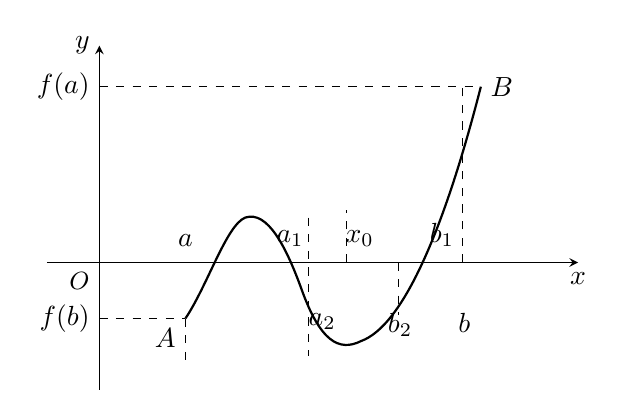
\begin{tikzpicture}[scale=0.95,>=stealth]
  \draw[->] (-0.7,0) -- (6.4,0) node[below] {$x$};
  \draw[->] (0,-1.7) -- (0,2.9) node[left] {$y$};
  \node[below left] at (0,0) {\small $O$};
  \draw[thick] (1.15,-0.75)
    .. controls (1.45,-0.30) and (1.70,0.50) .. (1.95,0.60)
    .. controls (2.25,0.70) and (2.50,0.20) .. (2.70,-0.35)
    .. controls (2.95,-1.05) and (3.20,-1.20) .. (3.50,-1.05)
    .. controls (4.05,-0.85) and (4.60,0.40) .. (5.10,2.35);
  \node[right] at (5.10,2.35) {$B$};
  \node[below left] at (1.15,-0.75) {$A$};
  \draw[dashed] (0,2.35) -- (5.10,2.35);
  \draw[dashed] (0,-0.75) -- (1.15,-0.75);
  \node[left] at (0,2.35) {$f(a)$};
  \node[left] at (0,-0.75) {$f(b)$};
  \draw[dashed] (1.15,-0.75) -- (1.15,-1.30);
  \node[above] at (1.15,0.08) {$a$};
  \draw[dashed] (2.80,0.60) -- (2.80,-1.25);
  \node[above] at (2.55,0.08) {$a_1$};
  \node[below] at (2.98,-0.55) {$a_2$};
  \draw[dashed] (3.30,0) -- (3.30,0.70);
  \node[above] at (3.48,0.08) {$x_0$};
  \draw[dashed] (4.00,0) -- (4.00,-0.70);
  \node[below] at (4.02,-0.55) {$b_2$};
  \draw[dashed] (4.85,0) -- (4.85,2.35);
  \node[above] at (4.58,0.08) {$b_1$};
  \node[below] at (4.88,-0.55) {$b$};
\end{tikzpicture}
\caption{}\label{fig:2.5.1}
\end{figure}

\begin{theoremp}[推广的零(根)值定理]\label{thm:2.5.1p}
设 $f$ 为 $[a,b]$ 上的连续函数, 且 $f(a)f(b) \leqslant 0$, 则 $\exists \xi \in [a,b]$, s.t. $f(\xi) = 0$.
\end{theoremp}

\begin{proof}
如果 $f(a) = 0$, 则取 $\xi = a$; 如果 $f(b) = 0$, 则取 $\xi = b$; 如果 $f(a)f(b) \neq 0$, 则 $f(a)f(b) < 0$, 由零值定理~\ref{thm:2.5.1} 知, $\exists \xi \in (a,b)$, s.t. $f(\xi) = 0$.
\end{proof}

\begin{theorem}[介值定理]\label{thm:2.5.2}
设 $f$ 为 $[a,b]$ 上的连续函数,\allowbreak $f(a) \neq f(b)$,\allowbreak 则 $\forall r \in (\min\{f(a), f(b)\},\allowbreak \max\{f(a), f(b)\})$, $\exists \xi \in (a,b)$, s.t. $f(\xi) = r$.
\end{theorem}

\begin{proof}
令 $F(x) = f(x) - r$, 显然它为 $[a,b]$ 上的连续函数, 且 $F(a)F(b) = (f(a) - r)(f(b) - r) < 0$. 由零值定理~\ref{thm:2.5.1} 知, $\exists \xi \in (a,b)$, s.t. $f(\xi) - r = F(\xi) = 0$, 即 $f(\xi) = r$(如图~\ref{fig:2.5.2} 所示).
\end{proof}

\begin{figure}[htbp]
\centering
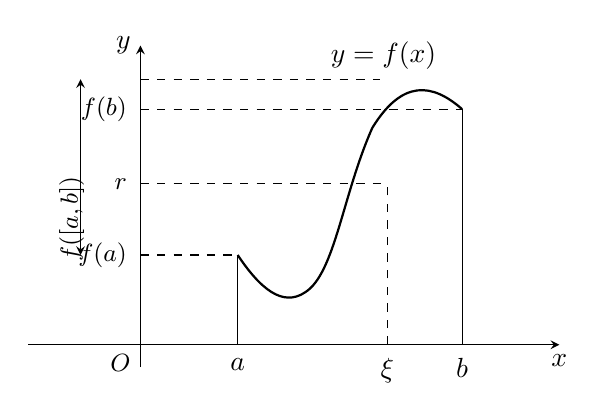
\begin{tikzpicture}[scale=0.95,>=stealth]
  \draw[->] (-1.5,0) -- (5.6,0) node[below] {$x$};
  \draw[->] (0,-0.3) -- (0,4.0) node[left] {$y$};
  \node[below left] at (0,0) {\small $O$};
  \draw[thick] (1.30,1.20)
    .. controls (1.60,0.75) and (1.90,0.50) .. (2.20,0.70)
    .. controls (2.60,0.95) and (2.70,2.00) .. (3.10,2.90)
    .. controls (3.50,3.55) and (3.90,3.50) .. (4.30,3.15);
  \node[above] at (3.25,3.55) {$y=f(x)$};
  \draw (1.30,1.20) -- (1.30,0);
  \draw (4.30,3.15) -- (4.30,0);
  \node[below] at (1.30,-0.05) {$a$};
  \node[below] at (4.30,-0.05) {$b$};
  \draw[dashed] (0,1.20) -- (1.32,1.20);
  \node[left,font=\small] at (-0.05,1.20) {$f(a)$};
  \draw[dashed] (0,3.15) -- (4.30,3.15);
  \node[left,font=\small] at (-0.05,3.15) {$f(b)$};
  \draw[dashed] (0,2.15) -- (3.30,2.15);
  \node[left,font=\small] at (-0.05,2.15) {$r$};
  \draw[dashed] (3.30,0) -- (3.30,2.15);
  \node[below] at (3.30,-0.05) {$\xi$};
  \draw[dashed] (0,3.55) -- (3.20,3.55);
  \draw[<->] (-0.80,1.20) -- (-0.80,3.55);
  \node[left,rotate=90,font=\small] at (-0.92,2.38) {$f([a,b])$};
\end{tikzpicture}
\caption{}\label{fig:2.5.2}
\end{figure}

\begin{theoremp}[推广的介值定理]\label{thm:2.5.2p}
设 $f$ 为 $[a,b]$ 上的连续函数,\allowbreak 则 $\forall r \in [\min\{f(a), f(b)\},\allowbreak \max\{f(a), f(b)\}]$, $\exists \xi \in [a,b]$, s.t. $f(\xi) = r$.
\end{theoremp}

\begin{proof}
不妨设 $f(a) \leqslant f(b)$. 如果 $r = \min\{f(a), f(b)\} = f(a)$, 则取 $\xi = a$; 如果 $r = \max\{f(a), f(b)\} = f(b)$, 则取 $\xi = b$. 如果 $f(a) = \min\{f(a), f(b)\} < r < \max\{f(a), f(b)\} = f(b)$, 则由介值定理~\ref{thm:2.5.2} 知, $\exists \xi \in (a,b)$, s.t. $f(\xi) = r$.

或者将推广的零值定理~\ref{thm:2.5.1p} 用于函数 $F(x) = f(x) - r$ 知, $\exists \xi \in [a,b]$, s.t. $0 = F(\xi) = f(\xi) - r$, 即 $f(\xi) = r$.
\end{proof}

\begin{corollary}\label{cor:2.5.1}
设 $f$ 为区间 $I$(开或半开半闭或闭)上的连续函数, 则 $f$ 的值域 $f(I) = \{f(x) \mid x \in I\}$ 也为一个区间(可退缩为一点).
\end{corollary}

\begin{proof}
若 $f$ 为常值函数, 即 $f(x) \equiv c$(常数), 则 $f(I) = \{c\}$ 退缩为一点.

若 $f$ 不为常值函数, 则必有 $y_1, y_2 \in f(I)$, s.t. $y_1 < y_2$. 由推广的介值定理~\ref{thm:2.5.2p} 知, $\forall r \in [y_1, y_2]$, 必 $\exists \xi \in I$, s.t. $r = f(\xi) \in f(I)$. 所以, $[y_1, y_2] \subset f(I)$. 由 $y_1, y_2$ 的任意性知, $f(I)$ 为一个区间.
\end{proof}

\begin{theorem}[最值定理]\label{thm:2.5.3}
设 $f$ 为有界闭区间 $[a,b]$ 上的连续函数, 则 $f$ 在 $[a,b]$ 上必达到最大值与最小值, 即必存在 $x_*, x^* \in [a,b]$, s.t.
\[
f(x_*) = \min_{x \in [a,b]} f(x) = m,
\]
\[
f(x^*) = \max_{x \in [a,b]} f(x) = M.
\]
\end{theorem}

\begin{proof}
记 $M = \sup\limits_{x \in [a,b]} f(x)$, 则 $M > -\infty$. 任取实数列 $\{\alpha_n\}$, s.t. $\alpha_n < M$ 且 $\{\alpha_n\}$ 严格增趋于 $M$. $\forall n \in \mathbb{N}$, $\alpha_n$ 不是 $f$ 在 $[a,b]$ 上的上界, 故 $\exists x_n \in [a,b]$, s.t. $\alpha_n < f(x_n) \leqslant M$. $\{x_n \mid n \in \mathbb{N}\} \subset [a,b]$ 为有界数列, 根据实数连续性命题(六)(序列紧性)知, 它有收敛子列 $x_{n_k}$. 令 $\lim\limits_{k \to +\infty} x_{n_k} = x^* \in [a,b]$, 由夹逼定理得到 $\lim\limits_{n \to +\infty} f(x_n) = \lim\limits_{n \to +\infty} \alpha_n = M$. 于是, 根据 $f$ 的连续性, 有
\[
M = \lim_{k \to +\infty} f(x_{n_k}) = f(x^*) \leqslant M,
\]
\[
f(x^*) = M,
\]
即 $f(x^*)$ 为 $f$ 在 $[a,b]$ 上的最大值.

同理可证, $\exists x_* \in [a,b]$, s.t. $f(x_*) = m = \inf\limits_{x \in [a,b]} f(x)$, 或用 $-f$ 代 $f$ 再应用上述所得结果.
\end{proof}

由此知, $f$ 在 $[a,b]$ 上为有界函数, 再由介值定理立即得到 $f$ 的值域
\[
f([a,b]) = \left[\min_{x \in [a,b]} f(x), \max_{x \in [a,b]} f(x)\right] = [m, M]
\]
为一个闭区间(包括退缩为一点, 此时 $f$ 为常值函数).

\begin{example}[不动点存在定理, Brouwer]\label{ex:2.5.1}
设 $f$ 在 $[a,b]$ 上连续, 满足 $a \leqslant f(x) \leqslant b, \forall x \in [a,b]$, 即 $f([a,b]) \subset [a,b]$, 则 $\exists \xi \in [a,b]$, s.t. $f(\xi) = \xi$, 称 $\xi$ 为 $f$ 的不动点.
\end{example}

\begin{proof}
令 $F(x) = f(x) - x$, 由 $f$ 连续知, $F$ 连续, 又因 $F(a)F(b) = (f(a) - a)(f(b) - b) \leqslant 0$, 根据推广零值定理~\ref{thm:2.5.1p} 知, $\exists \xi \in [a,b]$, s.t.
\[
f(\xi) - \xi = F(\xi) = 0,
\]
即 $f(\xi) = \xi$(如图~\ref{fig:2.5.3} 所示).
\end{proof}

\begin{figure}[htbp]
\centering
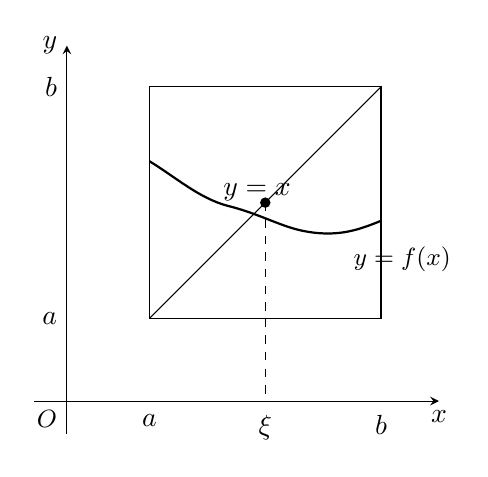
\begin{tikzpicture}[scale=1.05,>=stealth]
  \draw[->] (-0.4,0) -- (4.5,0) node[below] {$x$};
  \draw[->] (0,-0.4) -- (0,4.3) node[left] {$y$};
  \node[below left] at (0,0) {\small $O$};
  \draw (1.00,1.00) rectangle (3.80,3.80);
  \draw (1.00,1.00) -- (3.80,3.80);
  \node[above,sloped] at (2.30,2.30) {$y=x$};
  \draw[thick] (1.00,2.90)
    .. controls (1.30,2.72) and (1.60,2.45) .. (1.95,2.36)
    .. controls (2.35,2.26) and (2.60,2.10) .. (2.90,2.05)
    .. controls (3.30,1.98) and (3.55,2.08) .. (3.80,2.18);
  \node[below right,font=\small] at (3.35,1.98) {$y=f(x)$};
  \fill (2.40,2.40) circle (1.8pt);
  \draw[dashed] (2.40,2.40) -- (2.40,0);
  \node[below] at (1.00,-0.05) {$a$};
  \node[below] at (3.80,-0.05) {$b$};
  \node[below] at (2.40,-0.05) {$\xi$};
  \node[left] at (0,1.00) {$a$};
  \node[left] at (0,3.80) {$b$};
\end{tikzpicture}
\caption{}\label{fig:2.5.3}
\end{figure}

利用零值定理与介值定理可判断代数方程的根的存在范围.

\begin{example}\label{ex:2.5.2}
证明: 方程 $2^x = 4x$ 在 $\left(0, \frac{1}{2}\right)$ 中有根.
\end{example}

\begin{proof}
设 $f(x) = 2^x - 4x$, 它为初等函数, 因而是 $\left[0, \frac{1}{2}\right]$ 上的连续函数, 又 $f(0) = 2^0 - 4 \cdot 0 = 1 > 0$, $f\left(\frac{1}{2}\right) = 2^{\frac{1}{2}} - 4 \cdot \frac{1}{2} = \sqrt{2} - 2 < 0$, 则 $f(0)f\left(\frac{1}{2}\right) < 0$, 由零值定理~\ref{thm:2.5.1} 知, $\exists \xi \in \left(0, \frac{1}{2}\right)$, s.t.
\[
0 = f(\xi) = 2^{\xi} - 4\xi,
\]
即 $2^{\xi} = 4\xi, \xi \in \left(0, \frac{1}{2}\right)$ 为方程 $2^x = 4x$ 的一个根.
\end{proof}

\begin{example}\label{ex:2.5.3}
设 $f$ 在 $[a,b]$ 上连续, $x_1, x_2, \cdots, x_m \in [a,b]$, $\lambda_1, \lambda_2, \cdots, \lambda_m > 0$, $\sum\limits_{i=1}^{m} \lambda_i = 1$, 则 $\exists \xi \in [\min\{x_1, x_2, \cdots, x_m\}, \max\{x_1, x_2, \cdots, x_m\}] \subset [a,b]$, s.t.
\[
f(\xi) = \sum_{i=1}^{m} \lambda_i f(x_i).
\]
特别地, $\exists \xi \in [a,b]$, s.t. $f(\xi) = \frac{f(a) + f(b)}{2}$.
\end{example}

\begin{proof}
因为 $f$ 在 $[a,b]$ 上连续, 且
\[
\min\{f(x_1), f(x_2), \cdots, f(x_m)\} \leqslant \sum_{i=1}^{m} \lambda_i f(x_i) \leqslant \max\{f(x_1), f(x_2), \cdots, f(x_m)\},
\]
所以根据介值定理~\ref{thm:2.5.2} 知, $\exists \xi \in [\min\{x_1, x_2, \cdots, x_m\}, \max\{x_1, x_2, \cdots, x_m\}] \subset [a,b]$, s.t. $f(\xi) = \sum\limits_{i=1}^{m} \lambda_i f(x_i)$. 特别地, 当 $m = 2, x_1 = a, x_2 = b$, $\lambda_1 = \lambda_2 = \frac{1}{2}$ 时, $\exists \xi \in [a,b]$, s.t. $f(\xi) = \frac{f(a) + f(b)}{2}$.
\end{proof}

\begin{example}\label{ex:2.5.4}
证明: 实系数奇次多项式
\[
P(x) = x^{2n+1} + a_1 x^{2n} + \cdots + a_{2n} x + a_{2n+1}
\]
必有实根.
\end{example}

\begin{proof}
因为
\[
\lim_{x \to +\infty} P(x) = \lim_{x \to +\infty} x^{2n+1}\left(1 + \frac{a_1}{x} + \cdots + \frac{a_{2n}}{x^{2n}} + \frac{a_{2n+1}}{x^{2n+1}}\right) = +\infty,
\]
\[
\lim_{x \to -\infty} P(x) = \lim_{x \to -\infty} x^{2n+1}\left(1 + \frac{a_1}{x} + \cdots + \frac{a_{2n}}{x^{2n}} + \frac{a_{2n+1}}{x^{2n+1}}\right) = -\infty,
\]
故 $\exists \Delta > 0$, 当 $x > \Delta$ 时, $P(x) > 1$; 当 $x < -\Delta$ 时, $P(x) < -1$. 取 $a, b$, s.t. $a < -\Delta < \Delta < b$, 则 $P(a) < -1$, $P(b) > 1$. 又因多项式函数 $P(x)$ 为初等函数, 故它为 $\mathbb{R}$ 上的连续函数. 根据零值定理~\ref{thm:2.5.1}, $\exists \xi \in (a,b)$, s.t. $P(\xi) = 0$, 即实系数多项式 $P(x)$ 必有实根.
\end{proof}

\begin{example}\label{ex:2.5.5}
证明: $\tan x = x$ 有无穷个根.
\end{example}

\begin{proof}
设 $f(x) = \tan x - x, x \neq k\pi + \frac{\pi}{2}, k \in \mathbb{Z}$. 显然, 初等函数 $f(x) = \tan x - x$ 在其定义域中为连续函数, 因
\[
\lim_{x \to \left(k\pi + \frac{\pi}{2}\right)^-} (\tan x - x) = +\infty,
\]
\[
\lim_{x \to \left(k\pi - \frac{\pi}{2}\right)^+} (\tan x - x) = -\infty,
\]
故对每个固定的 $k \in \mathbb{Z}$, $\exists a_k, b_k$, s.t.
\[
k\pi - \frac{\pi}{2} < a_k < b_k < k\pi + \frac{\pi}{2},
\]
且 $f(a_k) < 0$, $f(b_k) > 0$. 根据零值定理~\ref{thm:2.5.1} 知, $\exists \xi_k \in (a_k, b_k) \subset \left(k\pi - \frac{\pi}{2}, k\pi + \frac{\pi}{2}\right)$, s.t.
\[
0 = f(\xi_k) = \tan \xi_k - \xi_k,
\]
即 $\tan \xi_k = \xi_k, k \in \mathbb{Z}$. 所以, $\tan x = x$ 有无穷个根(如图~\ref{fig:2.5.4} 所示).
\end{proof}

\begin{figure}[htbp]
\centering
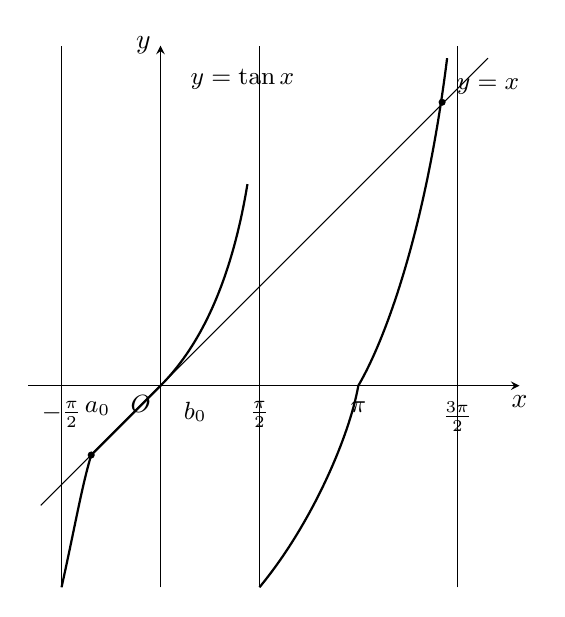
\begin{tikzpicture}[scale=0.80,>=stealth]
  \draw[->] (-2.1,0) -- (5.7,0) node[below] {$x$};
  \draw[->] (0,-3.2) -- (0,5.4) node[left] {$y$};
  \node[below left] at (0,0) {\small $O$};
  \draw (-1.571,-3.2) -- (-1.571,5.4);
  \draw (1.571,-3.2) -- (1.571,5.4);
  \draw (4.712,-3.2) -- (4.712,5.4);
  \draw[thick] (-1.571,-3.2)
     .. controls (-1.35,-2.20) and (-1.25,-1.60) .. (-1.10,-1.10)
     .. controls (-0.60,-0.60) and (-0.30,-0.30) .. (0,0)
     .. controls (0.55,0.55) and (1.10,1.50) .. (1.38,3.20);
  \draw[thick] (1.571,-3.2)
     .. controls (2.40,-2.20) and (3.00,-0.80) .. (3.14,0)
     .. controls (3.55,0.70) and (4.20,2.40) .. (4.55,5.20);
  \draw (-1.9,-1.9) -- (5.2,5.2);
  \node[right,font=\small] at (4.55,4.75) {$y=x$};
  \node[above,font=\small] at (1.30,4.55) {$y=\tan x$};
  \fill (-1.10,-1.10) circle (1.6pt);
  \fill (4.47,4.50) circle (1.6pt);
  \node[below,font=\small] at (-1.571,-0.10) {$-\frac{\pi}{2}$};
  \node[below,font=\small] at (-1.00,-0.10) {$a_0$};
  \node[below,font=\small] at (0.55,-0.10) {$b_0$};
  \node[below,font=\small] at (1.571,-0.10) {$\frac{\pi}{2}$};
  \node[below,font=\small] at (3.14,-0.10) {$\pi$};
  \node[below,font=\small] at (4.712,-0.10) {$\frac{3\pi}{2}$};
\end{tikzpicture}
\caption{}\label{fig:2.5.4}
\end{figure}

\begin{example}\label{ex:2.5.6}
设函数 $f$ 在 $(a,b)$ 上连续, 且 $f(a^+), f(b^-)$ 存在有限, 则 $f$ 在 $(a,b)$ 上有界.
\end{example}

\begin{proof}
\textbf{证法 1}\quad 令
\[
\tilde{f}(x) = \begin{cases} f(x), & x \in (a,b), \\ f(a^+), & x = a, \\ f(b^-), & x = b. \end{cases}
\]
显然, $\tilde{f}$ 在 $[a,b]$ 上连续, 根据最值定理~\ref{thm:2.5.3} 知, $\exists x_*, x^* \in [a,b]$, s.t. $\tilde{f}(x_*) = \min\limits_{x \in [a,b]} \tilde{f}(x) \leqslant f(x) \leqslant \max\limits_{x \in [a,b]} \tilde{f}(x) = \tilde{f}(x^*)$, $\forall x \in (a,b)$, 从而, $f$ 在 $(a,b)$ 上有界.

\textbf{证法 2}\quad 因 $f(a^+), f(b^-)$ 存在有限, 所以, 对 $\varepsilon_0 = 1$, $\exists \delta > 0$, s.t. $a < a + \delta < b - \delta < b$, 且
\[
f(a^+) - 1 < f(x) < f(a^+) + 1, \quad a < x < a + \delta,
\]
\[
f(b^-) - 1 < f(x) < f(b^-) + 1, \quad b - \delta < x < b.
\]
由 $f$ 在 $[a+\delta, b-\delta]$ 上连续, 并根据最值定理~\ref{thm:2.5.3} 知,
\[
|f(x)| \leqslant L, \forall x \in [a+\delta, b-\delta].
\]
所以, $|f(x)| \leqslant M = \max\{L, |f(a^+) - 1|, |f(a^+) + 1|, |f(b^-) - 1|, |f(b^-) + 1|\}$, 即 $f$ 在 $(a,b)$ 上有界.
\end{proof}

\begin{example}\label{ex:2.5.7}
设 $f$ 在 $(-\infty, +\infty)$ 上连续, 且 $\lim\limits_{x \to \infty} f(x)$ 存在有限, 则 $f$ 在 $(-\infty, +\infty)$ 上有界, 且 $f$ 在 $(-\infty, +\infty)$ 上必达到最大值或最小值.
\end{example}

\begin{proof}
设 $\lim\limits_{x \to \infty} f(x) = a \in \mathbb{R}$.

如果 $f(x) \equiv a, \forall x \in (-\infty, +\infty)$, 则 $f$ 在 $(-\infty, +\infty)$ 上有界, 且 $f$ 在其上达到最大值或最小值 $a$.

如果 $f(x) \not\equiv a$, 则 $\exists x_0 \in (-\infty, +\infty)$, s.t. $f(x_0) \neq a$.

若 $f(x_0) < a$, 取 $\varepsilon_0 \in (0, a - f(x_0))$, 因为 $\lim\limits_{x \to \infty} f(x) = a$, 故 $\exists \Delta > 0$, 当 $|x| > \Delta$ 时, 有 $f(x) > a - \varepsilon_0 > a - (a - f(x_0)) = f(x_0)$. 又因 $f$ 连续, 并根据最值定理~\ref{thm:2.5.3} 知, $\exists x_* \in [-\Delta, \Delta]$, s.t.
\[
f(x_*) = \min_{x \in [-\Delta, \Delta]} f(x) \leqslant f(x_0).
\]
于是(如图~\ref{fig:2.5.5} 所示),
\[
f(x_*) = \min_{x \in (-\infty, +\infty)} f(x).
\]
若 $f(x_0) > a$, 类似上述证明或用 $-f$ 代 $f$ 得 $x^* \in (-\infty, +\infty)$, s.t.
\[
f(x^*) = \max_{x \in (-\infty, +\infty)} f(x).
\]
\end{proof}

\begin{figure}[htbp]
\centering
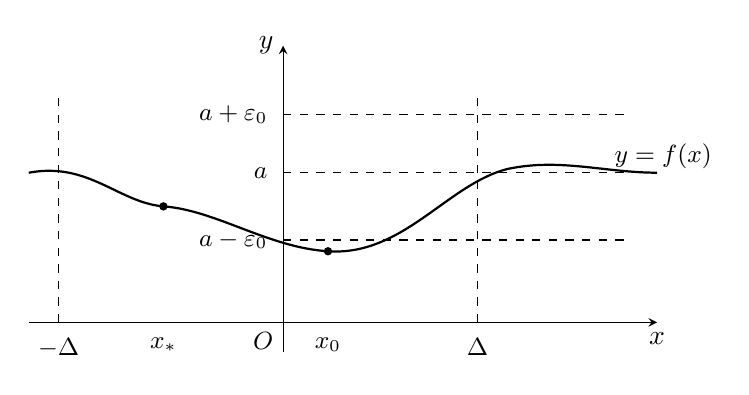
\begin{tikzpicture}[scale=0.95,>=stealth]
  \draw[->] (-3.4,0) -- (5.0,0) node[below] {$x$};
  \draw[->] (0,-0.4) -- (0,3.7) node[left] {$y$};
  \node[below left] at (0,0) {\small $O$};
  \draw[thick] (-3.4,2.00)
     .. controls (-2.60,2.15) and (-2.20,1.60) .. (-1.60,1.55)
     .. controls (-0.90,1.50) and (-0.20,1.00) .. (0.60,0.95)
     .. controls (1.60,0.88) and (2.20,1.85) .. (3.00,2.05)
     .. controls (3.70,2.20) and (4.30,2.00) .. (5.0,2.00);
  \node[right,font=\small] at (4.30,2.22) {$y=f(x)$};
  \draw[dashed] (0,2.00) -- (5.0,2.00);
  \draw[dashed] (0,2.78) -- (4.60,2.78);
  \draw[dashed] (0,1.10) -- (4.60,1.10);
  \node[left,font=\small] at (-0.08,2.00) {$a$};
  \node[left,font=\small] at (-0.08,2.78) {$a+\varepsilon_0$};
  \node[left,font=\small] at (-0.08,1.10) {$a-\varepsilon_0$};
  \draw[dashed] (-3.00,0) -- (-3.00,3.10);
  \draw[dashed] (2.60,0) -- (2.60,3.10);
  \node[below,font=\small] at (-3.00,-0.08) {$-\Delta$};
  \node[below,font=\small] at (2.60,-0.08) {$\Delta$};
  \fill (-1.60,1.55) circle (1.6pt);
  \node[below,font=\small] at (-1.60,-0.08) {$x_*$};
  \fill (0.60,0.95) circle (1.6pt);
  \node[below,font=\small] at (0.60,-0.08) {$x_0$};
\end{tikzpicture}
\caption{}\label{fig:2.5.5}
\end{figure}

为了讨论有界闭区间 $[a,b]$ 上另一个重要的一致连续性定理, 我们先引进一致连续的概念.

\begin{definition}\label{def:2.5.1}
设 $X \subsetneq \mathbb{R}$, $f\colon X \to \mathbb{R}$ 为一元函数. 如果 $\forall \varepsilon > 0$, $\exists \delta = \delta(\varepsilon) > 0$($\delta(\varepsilon)$ 只与 $\varepsilon$ 有关, 而与 $X$ 中的点 $x$ 无关!), 当 $x', x'' \in X$, 且 $x'$ 与 $x''$ 之间的距离 $\rho(x', x'') = |x' - x''|$ 小于 $\delta$, 就有 $|f(x') - f(x'')| < \varepsilon$, 则称 $f$ 在 $X$ 上是\textbf{一致连续}(或\textbf{均匀连续})的.
\end{definition}

\begin{theorem}\label{thm:2.5.4}
如果 $f$ 在 $X$ 上一致连续, 则 $f$ 在 $X$ 上连续. 但反之不真.
\end{theorem}

\begin{proof}
$\forall \varepsilon > 0$, 因 $f$ 在 $X$ 上一致连续, 故 $\exists \delta = \delta(\varepsilon) > 0$, 当 $x', x'' \in X, |x' - x''| < \delta$ 时, 有 $|f(x') - f(x'')| < \varepsilon$. 对 $x_0 \in X$, 当 $x \in X, |x - x_0| < \delta$ 时, 当然有 $|f(x) - f(x_0)| < \varepsilon$, 这就证明了 $f$ 在 $\forall x_0 \in X$ 处是连续的, 即 $f$ 在 $X$ 上连续.
\end{proof}

反之不真有反例: $f(x) = \frac{1}{x}$. 显然, 基本初等函数 $\frac{1}{x} = x^{-1}$ 在 $(0,1)$ 上连续. 但是, 它在 $(0,1)$ 上不一致连续.

\textbf{证法 1}\quad (反证) 假设 $f(x) = \frac{1}{x}$ 在 $(0,1)$ 上一致连续, 对 $\forall \varepsilon > 0, \exists \delta = \delta(\varepsilon) > 0$, 当 $x', x'' \in (0,1), |x' - x''| < \delta$ 时, 有
\[
\left|\frac{1}{x'} - \frac{1}{x''}\right| = |f(x') - f(x'')| < \varepsilon.
\]
取定 $x'' \in (0, \delta)$, 令 $x' \to 0^+$, 得到 $+\infty \leqslant \varepsilon$, 矛盾.

\textbf{证法 2}\quad 取 $\varepsilon_0 = 1, \forall \delta \in \left(0, \frac{1}{2}\right)$, 当 $x' = \frac{\delta}{2}, x'' = \delta$ 时, 虽然 $|x' - x''| = \left|\frac{\delta}{2} - \delta\right| = \frac{\delta}{2} < \delta$, 但
\[
\left|\frac{1}{x'} - \frac{1}{x''}\right| = \left|\frac{1}{\frac{\delta}{2}} - \frac{1}{\delta}\right| = \frac{1}{\delta} > 2 > 1 = \varepsilon_0.
\]
所以, $f(x) = \frac{1}{x}$ 在 $(0,1)$ 上不一致连续.

\textbf{证法 3}\quad 取 $x_n' = \frac{1}{n}, x_n'' = \frac{1}{n+1}$, 虽然
\[
|x_n' - x_n''| = \left|\frac{1}{n} - \frac{1}{n+1}\right| = \frac{1}{n(n+1)} \to 0 \quad (n \to +\infty),
\]
但
\[
|f(x_n') - f(x_n'')| = \left|\frac{1}{\frac{1}{n}} - \frac{1}{\frac{1}{n+1}}\right| = |n - (n+1)| = 1 \not\to 0 \quad (n \to +\infty).
\]
根据下面的定理~\ref{thm:2.5.8} 知, $f(x) = \frac{1}{x}$ 在 $(0,1)$ 上不一致连续.

\begin{theorem}[Cantor 定理]\label{thm:2.5.5}
有界闭区间 $[a,b]$ 上的连续函数是一致连续的.
\end{theorem}

\begin{proof}
\textbf{证法 1}\quad (反证) 假设 $f$ 在 $[a,b]$ 上不一致连续, 根据其定义知, $\exists \varepsilon_0 > 0, \forall n \in \mathbb{N}$, $\exists x_n', x_n'' \in [a,b]$, 虽然 $|x_n' - x_n''| < \frac{1}{n}$, 但
\[
|f(x_n') - f(x_n'')| \geqslant \varepsilon_0.
\]
由于数列 $\{x_n'\}$ 有界, 根据实数连续性命题(六)(序列紧性)知, 存在收敛子列 $\{x_{n_k}'\}$, 记
\[
\lim_{k \to +\infty} x_{n_k}' = x_0 \in [a,b].
\]
另一方面, 由于 $|x_{n_k}' - x_{n_k}''| < \frac{1}{n_k} \leqslant \frac{1}{k} \to 0\ (k \to +\infty)$, 故有 $\lim\limits_{k \to +\infty} x_{n_k}'' = x_0$, 但由上式知, $|f(x_{n_k}') - f(x_{n_k}'')| \geqslant \varepsilon_0$. 所以, 由 $f$ 连续得到
\[
0 = |f(x_0) - f(x_0)| = \lim_{k \to +\infty} |f(x_{n_k}') - f(x_{n_k}'')| \geqslant \varepsilon_0 > 0,
\]
矛盾.

\textbf{证法 2}\quad 因 $f$ 在 $[a,b]$ 上连续, 故 $\forall \varepsilon > 0, \forall x \in [a,b], \exists \delta_x > 0$, s.t. 当 $u \in [a,b] \cap (x - \delta_x, x + \delta_x)$ 时, $|f(u) - f(x)| < \frac{\varepsilon}{2}$. 当 $x', x'' \in [a,b] \cap (x - \delta_x, x + \delta_x)$ 时,
\[
\begin{aligned}
|f(x') - f(x'')| &\leqslant |f(x') - f(x)| + |f(x'') - f(x)| \\
&< \frac{\varepsilon}{2} + \frac{\varepsilon}{2} = \varepsilon.
\end{aligned}
\tag*{(*)}
\]
显然, $\mathcal{I} = \left\{\left(x - \frac{\delta_x}{2}, x + \frac{\delta_x}{2}\right) \mid x \in [a,b]\right\}$ 为 $[a,b]$ 的一个开区间覆盖. 由实数连续性命题(四)($[a,b]$ 的紧致性)知, 存在有限子覆盖 $\mathcal{I}_1 = \left\{\left(x_k - \frac{\delta_{x_k}}{2}, x_k + \frac{\delta_{x_k}}{2}\right) \mid k = 1, 2, \cdots, n\right\} \subset \mathcal{I}$. 令
\[
\delta = \delta(\varepsilon) = \min\left\{\frac{\delta_{x_k}}{2} \mid k = 1, 2, \cdots, n\right\} > 0,
\]
则 $\forall x', x'' \in [a,b], |x' - x''| < \delta$, $\exists k \in \mathbb{N}, 1 \leqslant k \leqslant n$, s.t.
\[
x' \in \left(x_k - \frac{\delta_{x_k}}{2}, x_k + \frac{\delta_{x_k}}{2}\right).
\]
于是,
\[
|x'' - x_k| \leqslant |x'' - x'| + |x' - x_k| < \delta + \frac{\delta_{x_k}}{2} \leqslant \delta_{x_k},
\]
即 $x'' \in (x_k - \delta_{x_k}, x_k + \delta_{x_k})$, 由 $(*)$ 式推得
\[
|f(x') - f(x'')| < \varepsilon,
\]
从而 $f$ 在 $[a,b]$ 上一致连续.

\textbf{证法 3}\quad 在证法 2 中, 令
\[
\tilde{\mathcal{I}} = \{(x - \delta_x, x + \delta_x) \mid x \in [a,b]\},
\]
则 $\tilde{\mathcal{I}}$ 为 $[a,b]$ 的开区间覆盖. 根据下面的 Lebesgue 数定理~\ref{thm:2.5.6} 知, 存在 Lebesgue 数 $\lambda = \lambda(\mathcal{I}) > 0$. $\forall \varepsilon > 0$, 取 $\delta = \delta(\varepsilon) = \lambda(\tilde{\mathcal{I}})$, 则当 $x', x'' \in [a,b]$ 且两点集 $\{x', x''\}$ 的直径为
\[
d(\{x', x''\}) = |x' - x''| < \delta = \lambda(\tilde{\mathcal{I}})
\]
时, 必有 $(x_0 - \delta_{x_0}, x_0 + \delta_{x_0}) \in \tilde{\mathcal{I}}$, s.t. $\{x', x''\} \subset (x_0 - \delta_{x_0}, x_0 + \delta_{x_0})$, 从而,
\[
|f(x') - f(x'')| < \varepsilon.
\]
这就证明了 $f$ 在 $[a,b]$ 上是一致连续的.
\end{proof}

\begin{theorem}[Lebesgue 数定理]\label{thm:2.5.6}
设 $\mathcal{I}$ 为有界闭区间 $[a,b]$ 上的一个开覆盖, 则必存在数 $\lambda = \lambda(\mathcal{I}) > 0$, 使当集合 $A \subset [a,b]$, 其直径 $d(A) = \sup\{\rho(x', x'') \mid x', x'' \in A\} < \lambda = \lambda(\mathcal{I})$ 时, 必有 $I \in \mathcal{I}$, s.t. $A \subset I$. 我们称 $\lambda = \lambda(\mathcal{I})$ 为 $\mathcal{I}$ 的一个 Lebesgue 数.
\end{theorem}

\begin{proof}
(反证) 假设结论不成立, 则 $\forall n \in \mathbb{N}$, 存在 $A_n \subset [a,b]$, 它的直径 $d(A_n) < \frac{1}{n}$, 而不存在 $I \in \mathcal{I}$, s.t. $A_n \subset I$. 在每个 $A_n$ 中取 $a_n$, 根据实数连续性命题(六)(序列紧性)可知, 存在子列 $\{a_{n_k}\}$ 收敛于 $a_0 \in [a,b]$. 因为 $\mathcal{I}$ 为 $[a,b]$ 的开覆盖, 故存在 $I_0 \in \mathcal{I}$, 使得 $a_0 \in I_0$. 因为 $I_0$ 为开集, 当 $[a,b] \setminus I_0 \neq \varnothing$ 时, 点 $a_0$ 到 $[a,b] \setminus I_0$ 的距离
\[
d = \rho(a_0, [a,b] \setminus I_0) = \inf\{\rho(a_0, x) \mid x \in [a,b] \setminus I_0\} > 0.
\]
由于 $\lim\limits_{k \to +\infty} a_{n_k} = a_0$, 所以, $\exists n_{k_0}$, s.t. $n_{k_0} > \frac{2}{d}$ 与 $\rho(a_0, a_{n_{k_0}}) < \frac{d}{2}$. 于是, $\forall x \in A_{n_{k_0}}$, 有
\[
\rho(a_0, x) \leqslant \rho(a_0, a_{n_{k_0}}) + \rho(a_{n_{k_0}}, x) < \frac{d}{2} + \frac{1}{n_{k_0}} < \frac{d}{2} + \frac{d}{2} = d,
\]
因而, $A_{n_{k_0}} \subset I_0 \in \mathcal{I}$; 当 $[a,b] \setminus I_0 = \varnothing$ 时, $A_n \subset [a,b] \subset I_0$, 这与不存在 $I \in \mathcal{I}$ 使得 $A_{n_{k_0}} \subset I$ 相矛盾.
\end{proof}

\begin{theorem}\label{thm:2.5.7}
$f$ 在 $(a,b)$ 上一致连续 $\iff f$ 可延拓为 $[a,b]$ 上的连续函数 $\tilde{f}$, 此时 $\tilde{f}|_{(a,b)} = f|_{(a,b)}$.
\end{theorem}

\begin{proof}
($\Leftarrow$) 设 $f$ 可延拓为 $[a,b]$ 上的连续函数 $\tilde{f}$, 由 Cantor 定理~\ref{thm:2.5.5} 知, $\tilde{f}$ 在 $[a,b]$ 上一致连续, 而 $\tilde{f}|_{(a,b)} = f|_{(a,b)}$, 因此 $f$ 在 $(a,b)$ 上一致连续.

($\Rightarrow$) 设 $f$ 在 $(a,b)$ 上一致连续. $\forall \varepsilon > 0$, $\exists \delta = \delta(\varepsilon) > 0$, 当 $x', x'' \in (a,b), |x' - x''| < \delta$ 时, $|f(x') - f(x'')| < \varepsilon$.

任取 $x_n \in (a,b)$, $x_n \to a^+$, 则 $\{x_n\}$ 为 Cauchy(基本)数列. 因此, $\exists N \in \mathbb{N}$, 当 $m, n > N$ 时, $|x_n - x_m| < \delta$, 从而有 $|f(x_n) - f(x_m)| < \varepsilon$. 这就证明了 $\{f(x_n)\}$ 为 Cauchy(基本)数列. 根据实数连续性命题(七)($\mathbb{R}$ 的完备性)知, $\{f(x_n)\}$ 收敛. $\forall x_n', x_n'' \to a^+\ (n \to +\infty)$, 显然有
\[
\{x_n'''\} \colon x_1', x_1'', x_2', x_2'', \cdots, x_n', x_n'', \cdots \to a^+.
\]
由上证得 $\{f(x_n''')\}$ 收敛, 并且
\[
\lim_{n \to +\infty} f(x_n') = \lim_{n \to +\infty} f(x_n'') = \lim_{n \to +\infty} f(x_n''').
\]
这就证明了 $\forall x_n \to a^+$, $\{f(x_n)\}$ 收敛于同一数, 故 $\lim\limits_{x \to a^+} f(x)$ 存在有限. 同理可证 $\lim\limits_{x \to b^-} f(x)$ 存在有限. 令
\[
\tilde{f}(x) = \begin{cases} f(a^+), & x = a, \\ f(x), & a < x < b, \\ f(b^-), & x = b. \end{cases}
\]
显然, $\tilde{f}$ 为 $[a,b]$ 上的连续函数, 且为 $f$ 的延拓.
\end{proof}

\begin{theorem}\label{thm:2.5.8}
设 $X \subsetneq \mathbb{R}$, $f\colon X \to \mathbb{R}$ 为一元函数. 如果 $\exists x_n', x_n'' \in X, n \in \mathbb{N}$, $|x_n' - x_n''| \to 0$ 但 $|f(x_n') - f(x_n'')| \not\to 0\ (n \to +\infty)$, 则 $f$ 在 $X$ 上不一致连续.
\end{theorem}

\begin{proof}
(反证) 假设 $f$ 在 $X$ 上一致连续, 则 $\forall \varepsilon > 0, \exists \delta = \delta(\varepsilon) > 0$, 当 $x', x'' \in X, |x' - x''| < \delta$ 时, $|f(x') - f(x'')| < \varepsilon$. 因 $|x_n' - x_n''| \to 0\ (n \to +\infty)$, 故 $\exists N \in \mathbb{N}$, 当 $n > N$ 时, $|x_n' - x_n''| < \delta$, 从而有
\[
|f(x_n') - f(x_n'')| < \varepsilon.
\]
由此就推得 $|f(x_n') - f(x_n'')| \to 0\ (n \to +\infty)$, 这与题设 $|f(x_n') - f(x_n'')| \not\to 0\ (n \to +\infty)$ 相矛盾.
\end{proof}

\begin{example}\label{ex:2.5.8}
设 $X \subsetneq \mathbb{R}$, $f\colon X \to \mathbb{R}$ 为一元函数, 它满足 Lipschitz 条件, 即 $\forall x', x'' \in X$, 有 $|f(x') - f(x'')| \leqslant M|x' - x''|$, 其中 $M$ 为常数, 则 $f$ 在 $X$ 上为一致连续函数.
\end{example}

\begin{proof}
$\forall \varepsilon > 0$, 取 $\delta \in \left(0, \frac{\varepsilon}{M+1}\right)$, 当 $x', x'' \in X$, 且 $|x' - x''| < \delta$ 时,
\[
|f(x') - f(x'')| \leqslant M|x' - x''| \leqslant M\delta < M \cdot \frac{\varepsilon}{M+1} < \varepsilon.
\]
因此, $f$ 在 $X$ 上为一致连续函数.
\end{proof}

\begin{example}\label{ex:2.5.9}
(1) $f(x) = \frac{1}{x}$ 在 $[a,b]$ 上一致连续, $0 < a < b$;

(2) $f(x) = ax + b$ 在 $(-\infty, +\infty)$ 内一致连续;

(3) $f(x) = x^2$ 在 $(-\infty, +\infty)$ 内不一致连续;

(4) $f(x) = \sin x^2$ 在 $(-\infty, +\infty)$ 内不一致连续;

(5) $f(x) = \sin \frac{1}{x}$ 在 $(0,1)$ 上不一致连续.
\end{example}

\begin{proof}
(1) $\forall \varepsilon > 0$, 取 $\delta \in (0, a^2\varepsilon)$, 当 $x', x'' \in [a,b], |x' - x''| < \delta$ 时,
\[
\left|\frac{1}{x'} - \frac{1}{x''}\right| = \frac{|x' - x''|}{x'x''} \leqslant \frac{|x' - x''|}{a^2} < \frac{\delta}{a^2} < \varepsilon,
\]
所以, $f(x) = \frac{1}{x}$ 在 $[a,b]$ 上一致连续.

(2) $\forall \varepsilon > 0$, 取 $\delta \in \left(0, \frac{\varepsilon}{|a|+1}\right)$, 当 $x', x'' \in (-\infty, +\infty), |x' - x''| < \delta$ 时,
\[
\begin{aligned}
|f(x') - f(x'')| &= |(ax' + b) - (ax'' + b)| = |ax' - ax''| \\
&= |a| \cdot |x' - x''| \leqslant (|a| + 1)\delta < \varepsilon,
\end{aligned}
\]
所以, $f(x) = ax + b$ 在 $(-\infty, +\infty)$ 内一致连续.

(3) 取 $x_n' = n, x_n'' = n + \frac{1}{n}$, 则 $|x_n' - x_n''| = \left|n - \left(n + \frac{1}{n}\right)\right| = \frac{1}{n} \to 0\ (n \to +\infty)$, 而
\[
|f(x_n') - f(x_n'')| = \left|n^2 - \left(n + \frac{1}{n}\right)^2\right| = 2 + \frac{1}{n^2} \to 2 \neq 0 \quad (n \to +\infty).
\]
根据定理~\ref{thm:2.5.8} 知, $f(x) = x^2$ 在 $(-\infty, +\infty)$ 内不一致连续.

(4) 取 $x_n' = \sqrt{2n\pi + \frac{\pi}{2}}, x_n'' = \sqrt{2n\pi}$, 则
\[
\begin{aligned}
|x_n' - x_n''| &= \left|\sqrt{2n\pi + \frac{\pi}{2}} - \sqrt{2n\pi}\right| \\
&= \frac{\frac{\pi}{2}}{\sqrt{2n\pi + \frac{\pi}{2}} + \sqrt{2n\pi}} \to 0 \quad (n \to +\infty),
\end{aligned}
\]
但
\[
\begin{aligned}
|f(x_n') - f(x_n'')| &= |\sin(x_n')^2 - \sin(x_n'')^2| \\
&= \left|\sin\left(2n\pi + \frac{\pi}{2}\right) - \sin 2n\pi\right| \\
&= |1 - 0| = 1 \not\to 0 \quad (n \to +\infty),
\end{aligned}
\]
根据定理~\ref{thm:2.5.8} 知, $f(x) = \sin x^2$ 在 $(-\infty, +\infty)$ 内不一致连续.

(5) \textbf{证法 1}\quad 取 $x_n' = \frac{1}{2n\pi}, x_n'' = \frac{1}{2n\pi + \frac{\pi}{2}}$, 则
\[
|x_n' - x_n''| = \left|\frac{1}{2n\pi} - \frac{1}{2n\pi + \frac{\pi}{2}}\right| = \frac{\frac{\pi}{2}}{2n\pi\left(2n\pi + \frac{\pi}{2}\right)} \to 0 \quad (n \to +\infty),
\]
但
\[
\begin{aligned}
|f(x_n') - f(x_n'')| &= \left|\sin\frac{1}{x_n'} - \sin\frac{1}{x_n''}\right| = \left|\sin 2n\pi - \sin\left(2n\pi + \frac{\pi}{2}\right)\right| \\
&= |0 - 1| = 1 \not\to 0 \quad (n \to +\infty),
\end{aligned}
\]
根据定理~\ref{thm:2.5.8} 知, $f(x) = \sin\frac{1}{x}$ 在 $(0,1)$ 上不一致连续.

\textbf{证法 2}\quad (反证) 假设 $f(x) = \sin\frac{1}{x}$ 在 $(0,1)$ 上一致连续, 由定理~\ref{thm:2.5.7} 知, $f(x)$ 可延拓为 $[0,1]$ 上的连续函数 $\tilde{f}(x)$, 因而 $\tilde{f}(0) = \lim\limits_{x \to 0^+} \tilde{f}(x) = \lim\limits_{x \to 0^+} \sin\frac{1}{x}$ 存在有限, 这与 $\lim\limits_{x \to 0^+} \sin\frac{1}{x}$ 显然不存在相矛盾.
\end{proof}

\begin{example}\label{ex:2.5.10}
设 $f$ 在 $[a,+\infty)$ 上连续, 且 $\lim\limits_{x \to +\infty} f(x)$ 存在有限, 则 $f$ 在 $[a,+\infty)$ 上一致连续.
\end{example}

\begin{proof}
\textbf{证法 1}\quad 因 $\lim\limits_{x \to +\infty} f(x) = A \in \mathbb{R}$, 故 $\forall \varepsilon > 0$, 必 $\exists \Delta > 0$, 当 $x > \Delta$ 时, 有 $|f(x) - A| < \frac{\varepsilon}{2}$.

又因 $f$ 连续, 根据 Cantor 定理~\ref{thm:2.5.5} 知, $f$ 在 $[a,\Delta]$ 上一致连续, 故 $\exists \delta_1 > 0$, 当 $x', x'' \in [a,\Delta], |x' - x''| < \delta_1$ 时, 有
\[
|f(x') - f(x'')| < \varepsilon.
\]
由于 $f$ 在点 $\Delta$ 处连续, 所以 $\exists \delta_2 > 0$, 当 $|x - \Delta| < \delta_2$ 时, 有
\[
|f(x) - f(\Delta)| < \frac{\varepsilon}{2}.
\]
令 $\delta = \min\{\delta_1, \delta_2\} > 0$, 当 $x', x'' \in [a,+\infty), |x' - x''| < \delta$ 时, 必有下面结论:

(1) $x', x'' \in (\Delta, +\infty)$, 则
\[
|f(x') - f(x'')| \leqslant |f(x') - A| + |f(x'') - A| < \frac{\varepsilon}{2} + \frac{\varepsilon}{2} = \varepsilon.
\]

(2) $x', x'' \in [a,\Delta]$, 则 $|f(x') - f(x'')| < \varepsilon$.

(3) $x' \in [a,\Delta], x'' \in [\Delta,+\infty)$, 则
\[
|x' - \Delta| < x'' - x' < \delta \leqslant \delta_2,
\]
\[
|f(x') - f(\Delta)| < \frac{\varepsilon}{2}.
\]
同理, $|f(x'') - f(\Delta)| < \frac{\varepsilon}{2}$. 因此,
\[
|f(x') - f(x'')| \leqslant |f(x') - f(\Delta)| + |f(x'') - f(\Delta)| < \frac{\varepsilon}{2} + \frac{\varepsilon}{2} = \varepsilon.
\]
这就证明了 $f$ 在 $[a,+\infty)$ 上是一致连续的.

\textbf{证法 2}\quad 因 $\lim\limits_{x \to +\infty} f(x) = A \in \mathbb{R}$, 故 $\forall \varepsilon > 0$, 必 $\exists \Delta > 0$, 当 $x > \Delta$ 时, 有 $|f(x) - A| < \frac{\varepsilon}{2}$.

又因 $f$ 连续, 根据 Cantor 定理~\ref{thm:2.5.5} 知, $f$ 在 $[a,\Delta+1]$ 上一致连续, 故 $\exists \delta_1 > 0$, 当 $x', x'' \in [a,\Delta+1], |x' - x''| < \delta_1$ 时, 有
\[
|f(x') - f(x'')| < \varepsilon.
\]
令 $\delta = \min\{1, \delta_1\}$, 当 $x', x'' \in [a,+\infty), x' < x'', |x' - x''| < \delta$ 时, 必有下面结论:

(1) $x', x'' \in (\Delta, +\infty)$, 则
\[
|f(x') - f(x'')| \leqslant |f(x') - A| + |f(x'') - A| < \frac{\varepsilon}{2} + \frac{\varepsilon}{2} = \varepsilon.
\]

(2) $x', x'' \in [a, \Delta+1]$, 则
\[
|f(x') - f(x'')| < \varepsilon.
\]

(3) 若 $a \leqslant x' < \Delta < \Delta + 1 < x''$, 则
\[
1 = (\Delta + 1) - \Delta < |x' - x''| < \delta \leqslant 1,
\]
矛盾. 由此推得这种情形不出现.

综合上述知, $f$ 在 $[a,+\infty)$ 上一致连续.
\end{proof}

\begin{example}\label{ex:2.5.11}
设 $f\colon (-\infty, +\infty) \to \mathbb{R}$ 是以 $T > 0$ 为周期的连续函数, 则 $f$ 在 $(-\infty, +\infty)$ 上一致连续.
\end{example}

\begin{proof}
\textbf{证法 1}\quad 因 $f$ 是以 $T > 0$ 为周期的函数, 根据 Cantor 定理~\ref{thm:2.5.5} 知, $\forall \varepsilon > 0, \exists \delta_1 > 0$, 当 $x', x'' \in [kT, (k+1)T], k \in \mathbb{Z}$ 时,
\[
|f(x') - f(x'')| < \varepsilon.
\]
$\forall kT, \exists \delta_2 > 0$, 当 $|x - kT| < \delta_2$ 时, 有
\[
|f(x) - f(kT)| < \frac{\varepsilon}{2}.
\]
于是, $\forall x', x'' \in (kT - \delta_2, kT + \delta_2)$,
\[
|f(x') - f(x'')| \leqslant |f(x') - f(kT)| + |f(x'') - f(kT)| < \frac{\varepsilon}{2} + \frac{\varepsilon}{2} = \varepsilon.
\]
令 $\delta = \min\{T, \delta_1, \delta_2\}$, 则当 $x', x'' \in (-\infty, +\infty)$, $x' \leqslant x''$, $|x' - x''| < \delta$ 时, 有下面结论:

(1) $x', x'' \in [kT, (k+1)T]$, 则 $|f(x') - f(x'')| < \varepsilon$;

(2) $x' \in [(k-1)T, kT], x'' \in [kT, (k+1)T]$, 则
\[
|x' - kT| \leqslant |x' - x''| < \delta \leqslant \delta_2,
\]
\[
|x'' - kT| \leqslant |x' - x''| < \delta \leqslant \delta_2,
\]
\[
|f(x') - f(x'')| < \varepsilon.
\]
这就证明了 $f$ 在 $(-\infty, +\infty)$ 上是一致连续的.

\textbf{证法 2}\quad 因 $f$ 在 $[0,2T]$ 内连续, 根据 Cantor 定理~\ref{thm:2.5.5} 知, $f$ 在 $[0,2T]$ 内一致连续, 故 $\forall \varepsilon > 0$, 取 $\delta_1 > 0$, 当 $x', x'' \in [0,2T], |x' - x''| < \delta_1$ 时, 有 $|f(x') - f(x'')| < \varepsilon$.

令 $\delta = \min\{T, \delta_1\}$, 当 $x', x'' \in (-\infty, +\infty)$, $x' < x''$, 且 $|x' - x''| < \delta$ 时, 必有 $n \in \mathbb{Z}$, s.t. $x' = nT + x_0'$, 其中 $x_0' \in [0, T]$, 则 $x'' = nT + x_0''$, $x_0'' \in [0, 2T]$. 于是, $|x_0' - x_0''| = |(x' - nT) - (x'' - nT)| = |x' - x''| < \delta$,
\[
|f(x') - f(x'')| = |f(x_0') - f(x_0'')| < \varepsilon.
\]
这就证明了 $f$ 在 $(-\infty, +\infty)$ 内一致连续.
\end{proof}

\begin{exblock}{练习题 2.5}
\item 用 $\varepsilon$-$\delta$ 语言表达函数 $f$ 在 $I$ 上不一致连续.

\item 设函数 $f$ 在开区间 $(a,b)$ 上连续且 $f(a^+)$ 与 $f(b^-)$ 存在有限. 证明: $f$ 在 $(a,b)$ 上一致连续.

\item 设函数 $f$ 在区间 $[a,+\infty)$ 上连续, 若存在常数 $b$ 与 $c$ 使得
  \[
  \lim_{x \to +\infty} (f(x) - bx - c) = 0,
\]
  则称直线 $y = bx + c$ 为曲线 $y = f(x)$ 的一条渐近线. 在这种情况下, $f$ 在 $[a,+\infty)$ 上一致连续.

\item 由"连续的周期函数一定是一致连续的"证明: $\sin^2 x + \sin x^2$ 不是周期函数.

\item 研究下列函数的一致连续性:
  \begin{enumerate}[label=(\arabic*)]
    \item $f(x) = \sin x, x \in \mathbb{R}$;
    \item $f(x) = \cos\frac{1}{x}, x > 0$;
    \item $f(x) = \sqrt[3]{x}, x \geqslant 0$;
    \item $f(x) = \cos x^2, x \in \mathbb{R}$;
    \item $f(x) = x\cos\frac{1}{x}, x > 0$;
    \item $f(x) = x\arctan x, x \in \mathbb{R}$;
    \item $f(x) = x^2\arcsin x, |x| \leqslant 1$.
  \end{enumerate}

\item 证明:
  \begin{enumerate}[label=(\arabic*)]
    \item 3 次方程 $x^3 + 2x - 1 = 0$ 只有唯一根, 此根在 $(0,1)$ 内;
    \item 方程 $x^5 - 3x + 1 = 0$ 在区间 $[0,1]$ 中有根;
    \item 方程 $x^{2x} = 1$ 在区间 $[0,1]$ 上有根;
    \item 方程 $\frac{a_1}{x - \lambda_1} + \frac{a_2}{x - \lambda_2} + \frac{a_3}{x - \lambda_3} = 0$, $a_1, a_2, a_3 > 0$, $\lambda_1 < \lambda_2 < \lambda_3$ 在区间 $(\lambda_1, \lambda_2)$ 与 $(\lambda_2, \lambda_3)$ 中各有一根;
    \item 实系数偶次多项式
      \[
      f(x) = x^{2n} + a_1 x^{2n-1} + \cdots + a_{2n-1}x + a_{2n}
\]
      当 $a_{2n} < 0$ 时至少有两个实根;
    \item 方程 $x - \lambda\sin x = 0\ (0 \leqslant \lambda < 1)$ 有惟一的根;
    \item 方程 $x - \lambda\sin x = b\ (0 \leqslant \lambda < 1, b > 0)$ 在 $[0, \lambda + b]$ 中有一根;
    \item 方程 $\sin x = \frac{1}{x}$ 有无穷多个根.
  \end{enumerate}

\item 证明: 存在惟一的连续函数 $f$, $\forall x \in \mathbb{R}, y = f(x)$ 满足 Kepler 方程:
  \[
  y - \lambda\sin y = x, \quad 0 \leqslant \lambda < 1.
\]

\item 设 $\varphi(x)$ 在 $\mathbb{R}$ 上连续, 且
  \[
  \lim_{x \to +\infty} \frac{\varphi(x)}{x^n} = \lim_{x \to -\infty} \frac{\varphi(x)}{x^n} = 0.
\]
  证明:
  \begin{enumerate}[label=(\arabic*)]
    \item 当 $n$ 为奇数时, 方程 $x^n + \varphi(x) = 0$ 有一实根;
    \item 当 $n$ 为偶数时, 存在数 $y$ 使得 $\forall x \in \mathbb{R}$, 有 $y^n + \varphi(y) \leqslant x^n + \varphi(x)$.
  \end{enumerate}

\item 设 $f$ 在 $\mathbb{R}$ 上连续, 且 $\forall x, y \in \mathbb{R}$, 函数 $f$ 满足:
  \[
  |f(x) - f(y)| \leqslant k|x - y|, \quad 0 < k < 1.
\]
  证明:
  \begin{enumerate}[label=(\arabic*)]
    \item 函数 $kx - f(x)$ 单调增;
    \item $\exists_1 \xi \in \mathbb{R}$, s.t. $f(\xi) = \xi$.
  \end{enumerate}

\item (1) 设 $f, g$ 在区间 $I$ 上一致连续. 证明: $f + g$ 在 $I$ 上也一致连续.

(2) 设区间 $I_1$ 以 $c$ 为右端点, 区间 $I_2$ 以 $c$ 为左端点. 证明: 函数 $f$ 在 $I_1 \cup I_2$ 上一致连续 $\iff f$ 在 $I_1$ 与 $I_2$ 上都一致连续.

\item (1) 证明: $f(x) = \sqrt{x}$ 在 $[0,+\infty)$ 上一致连续;

(2) 应用例~\ref{ex:2.5.11} 及 $\sin x' - \sin x'' = 2\cos\frac{x' + x''}{2}\sin\frac{x' - x''}{2}$, 证明: $f(x) = \sin x$ 在 $(-\infty, +\infty)$ 上一致连续;

(3) 证明: $f(x) = \cos\sqrt{x}$ 在 $[0,+\infty)$ 上一致连续.

\item 设 $f$ 在 $[a,b]$ 上连续, 且 $\forall x \in [a,b]$, $f(x) \neq 0$. 证明: $f$ 在 $[a,b]$ 上恒正或恒负.
\end{exblock}

\begin{exblock}{思考题 2.5}
\item 设函数 $f$ 在区间 $I$ 上连续, 且是一对一的(即有反函数), 则 $f$ 是严格单调的.

\item 设 $f\colon \mathbb{R} \to \mathbb{R}$ 连续, $f \circ f(x) = x, \forall x \in \mathbb{R}$. 证明: $\exists \xi \in \mathbb{R}$, s.t. $f(\xi) = \xi$.

\item 设 $f$ 在 $[a,b]$ 上连续 $(a < b)$, $f(a) = f(b)$. 证明: 在曲线 $y = f(x)\ (x \in [a,b])$ 上一定能找到两点 $A = (\xi, f(\xi))$, $B = \left(\xi + \frac{b-a}{2}, f\left(\xi + \frac{b-a}{2}\right)\right)$, 使得 $\xi \in \left[a, \frac{a+b}{2}\right]$ 且 $AB$ 平行 $x$ 轴.

\item 设 $f$ 在 $[0,2]$ 上连续, 且 $f(0) = f(2)$. 证明: $\exists \xi \in [0,1]$, 使得 $f(\xi) = f(\xi + 1)$.

\item 设 $f\colon [0,1] \to \mathbb{R}$ 连续, $f(0) = f(1)$. 证明: $\forall n \in \mathbb{N}$, 必存在 $\xi_n \in \left[0, 1 - \frac{1}{n}\right]$, 使得
  \[
  f(\xi_n) = f\left(\xi_n + \frac{1}{n}\right).
\]

\item 设函数 $f, g\colon [0,1] \to [0,1]$ 连续, 且 $\forall x \in [0,1]$ 有 $f(g(x)) = g(f(x))$. 证明:
  \begin{enumerate}[label=(\arabic*)]
    \item 如果 $f$ 单调减, 则 $\exists_1 a \in [0,1]$, s.t. $f(a) = g(a) = a$;
    \item 如果 $f$ 单调, 则 $\exists a \in [0,1]$, s.t. $f(a) = g(a) = a$;
    \item 如果 $f$ 单调增, 使 $f(a) = g(a) = a$ 成立的 $a \in [0,1]$ 是否惟一.
  \end{enumerate}

\item 设 $f\colon \mathbb{R} \to \mathbb{R}$ 为连续函数, 存在数 $a$ 及 $c > 0$, 使得对所有的 $n \in \mathbb{N}$ 有 $|f^n(a)| \leqslant c$. 证明: $f$ 有不动点 $x_0$, 即 $f(x_0) = x_0$. 这里 $f^n = f \circ f \circ \cdots \circ f$ 表示 $f$ 的 $n$ 次复合.

\item 设 $x_1, x_2, \cdots, x_n \in [0,1]$. 证明: $\exists t_0 \in [0,1]$, 使得
  \[
  \frac{1}{n}\sum_{i=1}^{n} |t_0 - x_i| = \frac{1}{2}.
\]

\item 设函数 $f$ 在区间 $I$ 上连续, 且有惟一的极值点 $x_0 \in \mathring{I}$($I$ 的内点集). 若 $f(x_0)$ 为极大(小)值, 则 $f(x_0)$ 为最大(小)值.

\item 设 $f$ 在 $[a,b)$ 上连续, $\lim\limits_{x \to b^-} f(x) = +\infty$, 且 $\forall (\alpha, \beta) \subset [a,b)$, $f(x)$ 在 $(\alpha, \beta)$ 上达不到最小值. 证明: $f$ 在 $[a,b)$ 上是严格增的.

\item 设 $f\colon \mathbb{R} \to \mathbb{R}$ 为连续函数, 且 $\forall x \in \mathbb{R}$ 都为 $f$ 的极值点. 证明: $f$ 为常值函数.

\item 设 $f$ 为 $\mathbb{R}$ 上的连续函数, 并且 $\lim\limits_{x \to \infty} f(x) = +\infty$, 又设 $f$ 的最小值 $f(a) < a$. 证明: $f \circ f$ 至少在两个点上达到最小值.
\end{exblock}

\begin{exblock}{复习题 2}
    \item 用记号 $C[a,b]$ 表示在区间 $[a,b]$ 上的连续函数的全体. 设 $f_i \in C[a,b]$, $i = 1, 2, 3$. 定义 $f(x)$ 为三个数 $f_1(x)$, $f_2(x)$, $f_3(x)$ 中介于中间的那一个. 证明: $f \in C[a,b]$.

    \item 设 $f$ 在 $(a,b)$ 上只有第 1 类间断点, 且 $\forall x, y \in (a,b)$ 有不等式
    \[
    f\left(\frac{x+y}{2}\right) \leqslant \frac{f(x) + f(y)}{2}.
\]
    证明: $f \in C(a,b)$.

    \item 对 $n \in \mathbb{N}$, 求满足函数方程
    \[
    f(x + y^n) = f(x) + (f(y))^n,\quad \forall x, y \in \mathbb{R}
\]
    的一切函数 $f$.

    \item 设 $f: \mathbb{R} \to \mathbb{R}$, 且 $f(x^2) = f(x)$, $\forall x \in \mathbb{R}$. 又 $f$ 在 $x = 0$ 与 $x = 1$ 处连续. 证明: $f$ 为常值函数.

    \item 定义函数 $f: [0,1] \to [0,1]$ 如下:
    \[
    f(x) = \begin{cases}
    0.0\, a_1\, 0\, a_2\, 0\, a_3 \cdots, & x = 0.a_1 a_2 a_3 \cdots,\\
    1, & x = 1,
\end{cases}
\]
    其中 $x = 0.a_1 a_2 a_3 \cdots$ 为 10 进制小数表示(当 $x$ 的 10 进制小数表示不惟一时, 一律采用有限小数的方法, 例如 $0.1$ 不表成 $0.0999\cdots$). 试讨论函数 $f$ 的连续性.

    \item 设函数 $f$ 在 $[0,+\infty)$ 上一致连续, 且 $\forall x \in [0,1]$ 有
    \[
    \lim_{n\to+\infty} f(x + n) = 0 \quad (n \in \mathbb{N}).
\]
    证明: $\lim\limits_{x\to+\infty} f(x) = 0$.

    \item 设 $I$ 为区间, 如果存在正的常数 $M$, 使得
    \[
    |f(x) - f(y)| \leqslant M|x - y|,\quad \forall x, y \in I,
\]
    则称 $f$ 在 $I$ 上满足 Lipschitz 条件. 证明: 如果 $f$ 在 $[a,+\infty)$ 满足 Lipschitz 条件 $(a > 0)$, 则 $\frac{f(x)}{x}$ 在 $[a,+\infty)$ 上一致连续.

    \item 证明: 函数 $f$ 在区间 $I$ 上一致连续 $\iff \forall \varepsilon > 0$, $\exists N \in \mathbb{N}$, s.t. 当 $x, y \in I$, $x \neq y$ 且
    \[
    \left|\frac{f(x) - f(y)}{x - y}\right| > N
\]
    时, 恒有 $|f(x) - f(y)| < \varepsilon$.

    \item 证明: 有理函数 $f(x) = \dfrac{1 + x^2}{1 - x^2 + x^4}$ 在 $\mathbb{R}$ 上有界. 进而证明上述有理函数 $f(x)$ 取到最大值 $1 + \dfrac{2}{3}\sqrt{3}$. 而下确界为 $0$, 不可达到.

    \item 设 $f$ 为 $\mathbb{R}$ 上的周期函数, 无最小正周期, 且 $f$ 在某点 $a$ 连续. 证明: $f$ 为常值函数. 换言之, 如果 $f$ 为无最小周期的周期函数且 $f$ 不为常值函数, 则 $f$ 处处不连续. (考察常值函数与 Dirichlet 函数.)

    \item 设函数 $f$ 与 $g$ 在 $[a,b]$ 上连续, 且有 $x_n \in [a,b]$, 使得
    \[
    g(x_n) = f(x_{n+1}),\quad n \in \mathbb{N}.
\]
    证明: 必有一点 $x_0 \in [a,b]$, 使 $f(x_0) = g(x_0)$.

    \item 设函数 $f$ 在区间 $[a,+\infty)$ 上连续有界. 证明: 对每一数 $\lambda$, 存在数列 $x_n \to +\infty$, 使
    \[
    \lim_{n\to+\infty} [f(x_n + \lambda) - f(x_n)] = 0.
\]

    \item 设函数 $f: \mathbb{R} \to \mathbb{R}$ 在有理点上取值为无理数, 在无理点上取值为有理数. 证明: $f$ 不为连续函数.

    \item 设 $f$ 为 $[a,b]$ 上的连续函数, 且在 $\forall [\alpha,\beta] \subset [a,b]$ 上至少有两个不同的最大值点. 证明: $f$ 在 $[a,b]$ 上为常值函数.

    \item 设 $S^2 = \{(x,y,z) \in \mathbb{R}^3 \mid x^2 + y^2 + z^2 = 1\}$ 为单位球面, $f: S^2 \to \mathbb{R}$ 为连续函数. 证明: $\exists \xi \in S^2$, 使 $f(\xi) = f(-\xi)$.

    \item (1) 在半径为 $1$ 的圆内有 $2005$ 个点 $P_1, P_2, \cdots, P_{2005}$. 证明: 在同一平面上一定存在这样一点 $P$, 它到这 $2005$ 个点的距离之和等于 $3000$;

    (2) 在单位球面 $S^2$ 上有 $2005$ 个点 $P_1, P_2, \cdots, P_{2005}$. 证明: 在此球面 $S^2$ 上必有一点 $P_0$, 使
    \[
    \sum_{i=1}^{2005} \widehat{P_0 P_i} = \frac{2005\pi}{2},
\]
    其中 $\widehat{P_0 P_i}$ 表示从 $P_0$ 到 $P_i$ 的球面距离, 即过 $P_0$ 与 $P_i$ 的大圆上, 以 $P_0$ 与 $P_i$ 为端点的劣弧之长.

    \item 设 $f(x)$ 在 $[a,b]$ 上连续, $f(a) < f(b)$. 又设 $\forall x \in (a,b)$, 有
    \[
    \lim_{t\to0} \frac{f(x+t) - f(x-t)}{t} = g(x)
\]
    存在且有限. 证明: $\exists c \in (a,b)$, s.t. $g(c) \geqslant 0$.

    \item 设函数 $f$ 在 $[0,+\infty)$ 上连续, $\forall \alpha > 0$, 有 $\lim\limits_{n\to+\infty} f(n\alpha) = 0$. 证明: $\lim\limits_{x\to+\infty} f(x) = 0$.

    \item 设 $\{f_n\}$ 为 $[a,b]$ 上的连续函数列, $f$ 为 $[a,b]$ 上的连续函数, 它们满足:
    \begin{enumerate}
        \item $f_1(x) \geqslant f_2(x) \geqslant \cdots$, $\forall x \in [a,b]$;
        \item $\lim\limits_{n\to+\infty} f_n(x) = f(x)$, $\forall x \in [a,b]$.
    \end{enumerate}
    证明: 函数序列 $\{f_n\}$ 在 $[a,b]$ 上一致收敛于 $f$.

    \item 设 $a(t)$, $b(t)$ 为 $[0,1]$ 上的连续函数, $0 \leqslant a(t) \leqslant \lambda < 1$. 证明: 方程
    \[
    x = \max_{0\leqslant t\leqslant1} \bigl[b(t) + x a(t)\bigr]
\]
    的解为
    \[
    x = \max_{0\leqslant t\leqslant1} \frac{b(t)}{1 - a(t)}.
\]

    \item (1) 证明: 不存在 $\mathbb{R}$ 上的连续函数, 使它的任一函数值都恰好被取到 $2$ 次;

    (2) 是否存在 $\mathbb{R}$ 上的连续函数, 使它的任一函数值都被恰好取到 $3$ 次.

    \item 设 $f$ 为 $\mathbb{R}$ 上的连续函数, 且 $\lim\limits_{x\to\infty} f \circ f(x) = \infty$. 证明: $\lim\limits_{x\to\infty} f(x) = \infty$.

    \item 应用夹逼定理或 $\ln(1 + x) = x + o(x)\ (x \to 0)$ 证明:
    \[
    \lim_{n\to+\infty} \left(1 + \frac{1^p}{n^{p+1}}\right) \cdots \left(1 + \frac{n^p}{n^{p+1}}\right) = \mathrm{e}^{\frac{1}{p+1}},\quad p > 0.
\]
\end{exblock}



% 第 3 章 一元函数的导数、微分中值定理（§3.1–§3.6 + 复习题 3）
% ====================================================================
%  徐森林、薛春华《数学分析》（第一册）
%  第 3 章  一元函数的导数、微分中值定理
%  源：原书印刷页 153-244（PDF 物理页 = 印刷页 + 6）
% ====================================================================

\chapter{一元函数的导数、微分中值定理}\label{ch:3}

从质点作直线运动的瞬时速度、直细棒的线密度、曲线切线的斜率出发引进导数概念; 进而再论述重要的 Fermat 定理、Rolle 定理、Lagrange 中值定理及 Cauchy 中值定理; 并应用这些定理研究函数的增减性、凹凸性、极值与最值; 给出求 $\frac{0}{0}$, $\frac{\infty}{\infty}$ 等不定型极限的 L'Hospital 法则.

% ====================================================================
%  徐森林、薛春华《数学分析》（第一册）
%  \S3.1  导数及其运算法则
%  源：原书印刷页 153-171（PDF 物理页 159-177）
%  底本：PaddleOCR-VL-1.6 + 高清影印比对校订
%  规范：全西文半角标点；单一落盘出口 _texout.py
% ====================================================================
\section{导数及其运算法则}\label{sec:3.1}

\begin{example}\label{ex:3.1.1}
设质点作直线运动, 在时刻 $t$ 的位移可用函数 $x = x(t)$ 来描述. 在时间段 $[t, t+\Delta t]$ 中位移的改变量为 $\Delta x = x(t+\Delta t) - x(t)$. 当 $\Delta t$ 很小时, 它在时刻 $t$ 的瞬时速度可近似地用它在 $[t, t+\Delta t]$ 中的平均速度
\[
\overline{v}(t,\Delta t) = \frac{\Delta x}{\Delta t} = \frac{x(t+\Delta t) - x(t)}{\Delta t}
\]
来代替. 如果当 $\Delta t \to 0$ 时, 极限
\[
v(t) = \lim_{\Delta t\to0}\frac{\Delta x}{\Delta t} = \lim_{\Delta t\to0}\frac{x(t+\Delta t) - x(t)}{\Delta t}
\]
存在有限, 则称它为质点在时刻 $t$ 的瞬时速度, 并记为 $v(t) = x'(t)$. 瞬时速度问题是微积分发明人之一——Newton 最早研究的.
\end{example}

\begin{example}\label{ex:3.1.2}
设直细棒从 $0$ 到 $x$ 一段的质量为 $m = m(x)$, 在 $[x, x+\Delta x]$ 一段的质量为 $\Delta m = m(x+\Delta x) - m(x)$. 当 $\Delta x$ 很小时, 在 $x$ 处的线密度可近似地用它在 $[x, x+\Delta x]$ 中的平均线密度
\[
\frac{\Delta m}{\Delta x} = \frac{m(x+\Delta x) - m(x)}{\Delta x}
\]
来代替. 如果当 $\Delta x \to 0$ 时, 极限
\[
\lim_{\Delta x\to0}\frac{\Delta m}{\Delta x} = \lim_{\Delta x\to0}\frac{m(x+\Delta x) - m(x)}{\Delta x}
\]
存在且有限, 则称它为直细棒在点 $x$ 处的线密度, 记为 $m'(x)$.
\end{example}

\begin{example}\label{ex:3.1.3}
设函数 $p = p(t)$ 表示某地区在时刻 $t$ 的人口数目, 则在时刻 $t+\Delta t$ 的人口数目就是 $p(t+\Delta t)$. 因此, 这个地区在从 $t$ 到 $t+\Delta t$ 的时间段中, 人口平均增长速度为
\[
\frac{\Delta p}{\Delta t} = \frac{p(t+\Delta t) - p(t)}{\Delta t}.
\]
如果当 $\Delta t \to 0$ 时, 极限
\[
\lim_{\Delta t\to0}\frac{\Delta p}{\Delta t} = \lim_{\Delta t\to0}\frac{p(t+\Delta t) - p(t)}{\Delta t}
\]
存在且有限, 则称它为该地区在时刻 $t$ 的人口增长速率, 并记为 $p'(t)$.
\end{example}

\begin{example}\label{ex:3.1.4}
设 $(x, f(x))$ 为曲线 $y = f(x)$ 上的一个定点, 而 $(x+\Delta x, f(x+\Delta x))$ 为该曲线上的一个动点. 显然, 通过点 $(x, f(x))$ 与 $(x+\Delta x, f(x+\Delta x))$ 的割线的斜率为
\[
\frac{\Delta y}{\Delta x} = \frac{f(x+\Delta x) - f(x)}{\Delta x},
\]
它是 $[x, x+\Delta x]$ 上函数 $y = f(x)$ 的平均变化率. 如果当 $\Delta x \to 0$ 时, 极限
\[
\lim_{\Delta x\to0}\frac{\Delta y}{\Delta x} = \lim_{\Delta x\to0}\frac{f(x+\Delta x) - f(x)}{\Delta x}
\]
存在且有限, 则称它为函数 $y = f(x)$ 在 $x$ 处的变化率, 记为 $f'(x)$, 并称它为 $f(x)$ 在 $x$ 处的导数. 称过点 $(x, f(x))$ 斜率为 $f'(x)$ 的直线(即割线的极限位置)为该点处的切线. 在图~\ref{fig:3.1.1} 中, $\frac{\Delta y}{\Delta x} = \tan\varphi$, $f'(x) = \lim\limits_{\Delta x\to0}\frac{\Delta y}{\Delta x} = \tan\varphi_0$.

由此进而可得, 曲线 $y = f(x)$ 在点 $(x_0, f(x_0))$ 处的切线方程为
\[
y - f(x_0) = f'(x_0)(x - x_0).
\]
过点 $(x_0, f(x_0))$ 且与切线垂直的直线称为曲线 $y = f(x)$ 在点 $(x_0, f(x_0))$ 处的法线. 于是, 当 $f'(x_0) \neq 0$ 时, 在点 $(x_0, f(x_0))$ 处法线为
\[
y - f(x_0) = -\frac{1}{f'(x_0)}(x - x_0);
\]
当 $f'(x_0) = 0$ 时, 在点 $(x_0, f(x_0))$ 处法线为 $x = x_0$. 两种情形统一表达为
\[
(x - x_0) + f'(x_0)(y - f(x_0)) = 0.
\]
Leibniz 的巨大贡献之一, 就是发现了曲线的切线斜率与函数的导数之间的联系, 同时得到了计算导数的一般方法. 下面来正式引进导数的概念.
\end{example}

\begin{figure}[htbp]
\centering
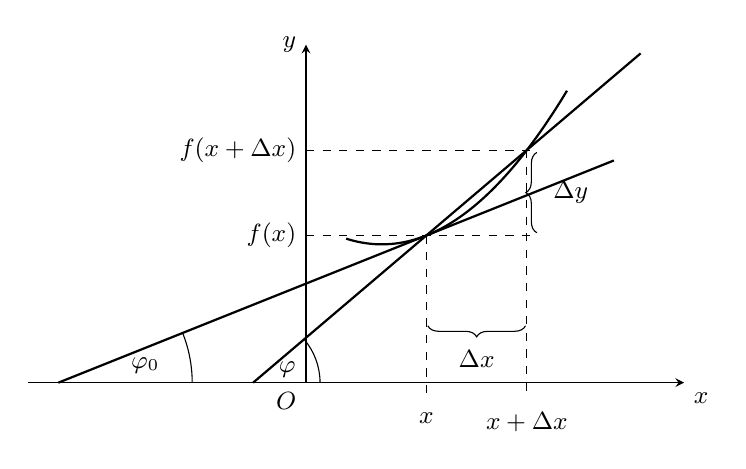
\begin{tikzpicture}[scale=0.85,>=stealth,font=\small]
  % 坐标轴
  \draw[->] (-3.15,0) -- (6.65,0) node[below right] {$x$};
  \draw[->] (1.0,0) -- (1.0,5.05) node[left] {$y$};
  \node[below left] at (1.0,0) {$O$};
  % 曲线 y=f(x)
  \draw[thick] plot[domain=1.6:4.9,samples=60,smooth]
    (\x,{0.30*(\x-2.8)*(\x-2.8)+0.40*(\x-2.8)+2.2});
  % 切线 (过 P(2.8,2.2), 斜率 0.40, 交 x 轴于 (-2.7,0))
  \draw[thick] (-2.7,0) -- (5.6,3.32);
  % 割线 PQ (斜率 0.85, 交 x 轴于 (0.21,0))
  \draw[thick] (0.21,0) -- (6.0,4.92);
  % 虚线
  \draw[dashed] (1.0,2.2) -- (4.45,2.2);
  \draw[dashed] (1.0,3.475) -- (4.45,3.475);
  \draw[dashed] (2.8,2.2) -- (2.8,-0.22);
  \draw[dashed] (4.3,3.475) -- (4.3,-0.22);
  % 纵坐标标注
  \node[left] at (1.0,2.2) {$f(x)$};
  \node[left] at (1.0,3.475) {$f(x+\Delta x)$};
  % 横坐标标注
  \node[below] at (2.8,-0.30) {$x$};
  \node[below] at (4.3,-0.30) {$x+\Delta x$};
  % Delta x 括号
  \draw[decorate,decoration={brace,amplitude=4pt,mirror}]
    (2.82,0.85) -- (4.28,0.85);
  \node at (3.55,0.36) {$\Delta x$};
  % Delta y 括号
  \draw[decorate,decoration={brace,amplitude=4pt}]
    (4.45,2.24) -- (4.45,3.44);
  \node[right] at (4.55,2.84) {$\Delta y$};
  % 角 φ0 (切线与 x 轴夹角)
  \draw (-2.7,0) ++(2.0,0) arc (0:21.8:2.0);
  \node at (-1.40,0.26) {$\varphi_0$};
  % 角 φ (割线与 x 轴夹角)
  \draw (0.21,0) ++(1.0,0) arc (0:40.4:1.0);
  \node at (0.72,0.20) {$\varphi$};
\end{tikzpicture}
\caption{}\label{fig:3.1.1}
\end{figure}

\begin{definition}[导数]\label{def:3.1.1}
设函数 $y = f(x)$ 在点 $x_0$ 处的某开邻域 $(x_0 - \delta_0, x_0 + \delta_0)$ (点 $x_0$ 附近)有定义. 如果极限
\[
\lim_{x\to x_0}\frac{f(x) - f(x_0)}{x - x_0} = \lim_{\Delta x\to0}\frac{f(x_0+\Delta x) - f(x_0)}{\Delta x} = \lim_{\Delta x\to0}\frac{\Delta y}{\Delta x}
\]
存在且有限, 则称函数 $f$ 在点 $x_0$ 处可导, 且称此极限值为 $f$ 在点 $x_0$ 处的导数(或变化率), 记为
\[
f'(x_0)\ \text{或}\ f'(x)|_{x=x_0}\ \text{或}\ \frac{\mathrm{d}f}{\mathrm{d}x}\Big|_{x=x_0}\ \text{或}\ y'(x_0)\ \text{或}\ \frac{\mathrm{d}y}{\mathrm{d}x}\Big|_{x=x_0},
\]
其中, $\Delta x = x - x_0$ 称为自变量 $x$ 的增量, 而 $\Delta y = f(x_0+\Delta x) - f(x_0)$ 称为函数(因变量)$y$ 的增量, $\frac{\Delta y}{\Delta x}$ 称为平均变化率.
\end{definition}

由定义~\ref{def:3.1.1} 知, 瞬时速度就是质点作直线运动的位移函数 $x(t)$ 对时间 $t$ 的导数; 直细棒的线密度就是其质量函数 $m(x)$ 对 $x$ 的导数, 这就是导数的物理意义. 切线的斜率就是 $y = f(x)$ 对 $x$ 的导数, 这是导数的几何意义.

用"$\varepsilon$-$\delta$"语言描述导数如下: $\forall \varepsilon > 0, \exists \delta > 0$, 当 $0 < |x - x_0| < \delta$ 时,
\[
\left|\frac{f(x) - f(x_0)}{x - x_0} - f'(x_0)\right| < \varepsilon,
\]
\[
\left|\frac{f(x_0+\Delta x) - f(x_0)}{\Delta x} - f'(x_0)\right| < \varepsilon.
\]

设 $f$ 在点 $x_0$ 的左旁 $(x_0 - \delta_0, x_0]$ 有定义, 如果
\[
\lim_{x\to x_0^-}\frac{f(x) - f(x_0)}{x - x_0} = \lim_{\Delta x\to0^-}\frac{f(x_0+\Delta x) - f(x_0)}{\Delta x}
\]
存在且有限, 则称此极限值为 $f$ 在点 $x_0$ 处的左导数, 记为 $f'_-(x_0)$. 类似可定义 $f$ 在点 $x_0$ 处的右导数 $f'_+(x_0)$.

\begin{theorem}\label{thm:3.1.1}
$f$ 在点 $x_0$ 处可导 $\iff f$ 在点 $x_0$ 处既左可导又右可导, 且 $f'_-(x_0) = f'_+(x_0)$.
\end{theorem}

\begin{proof}
$f$ 在点 $x_0$ 处可导, 即
\[
\lim_{x\to x_0}\frac{f(x) - f(x_0)}{x - x_0} = f'(x_0) \in \mathbb{R}
\]
\[
\iff f'_-(x_0) = \lim_{x\to x_0^-}\frac{f(x) - f(x_0)}{x - x_0} = \lim_{x\to x_0^+}\frac{f(x) - f(x_0)}{x - x_0} = f'_+(x_0) \in \mathbb{R},
\]
且 $f'_-(x_0) = f'(x_0) = f'_+(x_0)$.
\end{proof}

\begin{definition}\label{def:3.1.2}
如果 $y = f(x)$ 在开区间 $(a,b)$ 内的任一点 $x$ 处可导, 则称 $f$ 在 $(a,b)$ 内可导; 如果 $f$ 在有界区间 $(a,b)$ 内可导, 又在 $a$ 处右可导, 在 $b$ 处左可导, 则称 $f$ 在闭区间 $[a,b]$ 上可导.
\end{definition}

$f(x)$ 在区间 $I$ 中的导数形成一个新函数 $f'(x)$, 称为 $f(x)$ 的导函数. 如果 $f'(x)$ 为 $I$ 上的连续函数, 即 $\lim\limits_{x\to x_0}f'(x) = f'(x_0)$, $\forall x_0 \in I$, 则称 $f$ 为 $1$ 阶连续可导的函数.

注意, $f'_-(x_0)$ ($f'_+(x_0)$)为 $f$ 在点 $x_0$ 处的左(右)导数, 但是 $f'(x_0^-) = \lim\limits_{x\to x_0^-}f'(x)$ ($f'(x_0^+) = \lim\limits_{x\to x_0^+}f'(x)$)为导函数 $f'(x)$ 在点 $x_0$ 处的左(右)极限.

\begin{theorem}\label{thm:3.1.2}
设 $f$ 在点 $x_0$ 处可导, 则 $f$ 在点 $x_0$ 处连续. 反之不真.
\end{theorem}

\begin{proof}
($\Rightarrow$) 设 $f$ 在点 $x_0$ 处可导, 则
\[
\lim_{x\to x_0}f(x) = \lim_{x\to x_0}\left[\frac{f(x) - f(x_0)}{x - x_0}(x - x_0) + f(x_0)\right] = f'(x_0)\cdot0 + f(x_0) = f(x_0).
\]
这就证明了 $f$ 在点 $x_0$ 处连续.

($\Leftarrow$) 反例: $f(x) = |x|$ 在 $x_0 = 0$ 处连续, 但在 $x_0 = 0$ 处不可导.

事实上, 由
\[
f'_+(0) = \lim_{x\to0^+}\frac{f(x) - f(0)}{x - 0} = \lim_{x\to0^+}\frac{x - 0}{x - 0} = \lim_{x\to0^+}1 = 1
\]
\[
\neq -1 = \lim_{x\to0^-}(-1) = \lim_{x\to0^-}\frac{(-x) - 0}{x - 0} = \lim_{x\to0^-}\frac{f(x) - f(0)}{x - 0} = f'_-(0)
\]
及定理~\ref{thm:3.1.1} 得到: $f$ 在 $x_0 = 0$ 处不可导.
\end{proof}

\begin{theorem}[求导的四则运算法则]\label{thm:3.1.3}
设 $f$, $g$ 在点 $x$ 处可导, 则 $f \pm g$, $cf$($c$ 为常数), $fg$, $\frac{f}{g}$($g(x) \neq 0$)都在点 $x$ 处可导, 且
\begin{enumerate}[label=(\arabic*)]
  \item $(f \pm g)' = f' \pm g'$ (线性性);
  \item $(cf)' = cf'$ (线性性);
  \item $(fg)' = f'g + fg'$;
  \item $\left(\frac{f}{g}\right)' = \frac{f'g - fg'}{g^2}$.
\end{enumerate}
\end{theorem}

\begin{proof}
(1)
\[
\begin{aligned}
(f \pm g)'(x) &= \lim_{\Delta x\to0}\frac{(f \pm g)(x+\Delta x) - (f \pm g)(x)}{\Delta x}\\
&= \lim_{\Delta x\to0}\frac{[f(x+\Delta x) - f(x)] \pm [g(x+\Delta x) - g(x)]}{\Delta x}\\
&= f'(x) \pm g'(x).
\end{aligned}
\]
(2)
\[
\begin{aligned}
(cf)'(x) &= \lim_{\Delta x\to0}\frac{(cf)(x+\Delta x) - (cf)(x)}{\Delta x}\\
&= c\lim_{\Delta x\to0}\frac{f(x+\Delta x) - f(x)}{\Delta x} = cf'(x).
\end{aligned}
\]
(3) 由 $g$ 在点 $x$ 处可导及定理~\ref{thm:3.1.2} 推得 $g$ 在点 $x$ 处连续, 于是有
\[
\begin{aligned}
(fg)'(x) &= \lim_{\Delta x\to0}\frac{(fg)(x+\Delta x) - (fg)(x)}{\Delta x}\\
&= \lim_{\Delta x\to0}\frac{[f(x+\Delta x) - f(x)]g(x+\Delta x) + f(x)[g(x+\Delta x) - g(x)]}{\Delta x}\\
&= f'(x)g(x) + f(x)g'(x).
\end{aligned}
\]
(4) 同 (3) 知, $g$ 在点 $x$ 处连续, 故有
\[
\begin{aligned}
\left(\frac{f}{g}\right)'(x) &= \lim_{\Delta x\to0}\frac{\left(\frac{f}{g}\right)(x+\Delta x) - \left(\frac{f}{g}\right)(x)}{\Delta x}\\
&= \lim_{\Delta x\to0}\frac{1}{\Delta x}\left[\frac{f(x+\Delta x)}{g(x+\Delta x)} - \frac{f(x)}{g(x)}\right]\\
&= \lim_{\Delta x\to0}\frac{1}{g(x+\Delta x)g(x)}\\
&\quad\times\frac{[f(x+\Delta x) - f(x)]g(x+\Delta x) - f(x)[g(x+\Delta x) - g(x)]}{\Delta x}\\
&= \frac{f'(x)g(x) - f(x)g'(x)}{g^2(x)}.
\end{aligned}
\]
\end{proof}

\begin{theorem}[复合函数的求导链式规则, 简称链规则]\label{thm:3.1.4}
设 $y = y(u)$ 在点 $u_0$ 处可导, $u = u(x)$ 在点 $x_0$ 处可导, $u_0 = u(x_0)$, 则复合函数 $y = y(u(x)) = (y \circ u)(x)$ 在点 $x_0$ 处可导, 且
\[
\left(y(u(x))\right)'|_{x=x_0} = y'(u_0)u'(x_0),
\]
或
\[
y'_x|_{x=x_0} = y'_u|_{u=u_0}\cdot u'_x|_{x=x_0}.
\]
\end{theorem}

\begin{proof}
令
\[
F(\Delta u) = \begin{cases}
\dfrac{y(u_0+\Delta u) - y(u_0)}{\Delta u}, & \Delta u \neq 0,\\
y'(u_0), & \Delta u = 0,
\end{cases}
\]
则 $F(\Delta u)$ 在 $\Delta u = 0$ 处连续. 此外, 由 $u = u(x)$ 在点 $x_0$ 处可导知, $\Delta u \to 0\ (\Delta x \to 0)$. 于是,
\[
\begin{aligned}
(y(u(x)))'|_{x=x_0} &= \lim_{\Delta x\to0}\frac{y(u(x_0+\Delta x)) - y(u(x_0))}{\Delta x}\\
&= \lim_{\Delta x\to0}F(\Delta u)\cdot\frac{\Delta u}{\Delta x} = y'(u_0)u'(x_0).
\end{aligned}
\]
\end{proof}

\begin{theorem}[反函数的求导法则]\label{thm:3.1.5}
设 $y = f(x)$ 为 $x = g(y)$ 的反函数(即 $f = g^{-1}$, $g = f^{-1}$). 如果 $g(y)$ 在点 $y_0$ 的某开邻域内连续、严格单调且 $g'(y_0) \neq 0$, 则 $f(x)$ 在点 $x_0 = g(y_0)$ 处可导, 且
\[
f'(x_0) = \frac{1}{g'(y_0)} = \frac{1}{(f^{-1}(y))'|_{y=y_0}},\ \text{或}\ y'_x(x_0) = \frac{1}{x'_y(y_0)}.
\]
\end{theorem}

\begin{proof}
因为 $g$ 在点 $y_0$ 的某开邻域内连续且严格单调, 根据定理~\ref{thm:2.4.4} 知, $f = g^{-1}$ 在点 $x_0$ 的某开邻域内连续且严格单调, 从而
\[
\Delta y = f(x_0+\Delta x) - f(x_0) = 0 \iff \Delta x = g(y_0+\Delta y) - g(y_0) = 0,\quad \Delta y \to 0 \iff \Delta x \to 0.
\]
由 $g'(y_0) \neq 0$, 可得
\[
f'(x_0) = \lim_{\Delta x\to0}\frac{\Delta y}{\Delta x} = \lim_{\Delta x\to0}\frac{1}{\frac{\Delta x}{\Delta y}} = \frac{1}{g'(y_0)}.
\]
\end{proof}

\begin{example}\label{ex:3.1.5}
证明下列基本初等函数的导数:
\begin{enumerate}[label=(\arabic*)]
  \item $C' = 0$, 其中 $C$ 为常值函数;
  \item $(\sin x)' = \cos x$, $(\cos x)' = -\sin x$, $(\tan x)' = \sec^2 x$, $(\cot x)' = -\csc^2 x$, $(\sec x)' = \sec x\tan x$, $(\csc x)' = -\csc x\cot x$;
  \item $(\log_a x)' = \frac{1}{x\ln a}\ (a>0)$, $(\ln x)' = \frac{1}{x}$, $(\ln|x|)' = \frac{1}{x}$;
  \item $(x^\mu)' = \mu x^{\mu-1}$;
  \item $(a^x)' = a^x\ln a$, $(\mathrm{e}^x)' = \mathrm{e}^x$;
  \item $(\arcsin x)' = \frac{1}{\sqrt{1-x^2}}$, $(\arccos x)' = -\frac{1}{\sqrt{1-x^2}}$, $(\arctan x)' = \frac{1}{1+x^2}$, $(\operatorname{arccot} x)' = -\frac{1}{1+x^2}$.
\end{enumerate}
\end{example}

\begin{proof}
(1) $C' = \lim\limits_{\Delta x\to0}\frac{C - C}{\Delta x} = \lim\limits_{\Delta x\to0}0 = 0$.

(2)
\[
\begin{aligned}
(\sin x)' &= \lim_{\Delta x\to0}\frac{\sin(x+\Delta x) - \sin x}{\Delta x} = \lim_{\Delta x\to0}\frac{2\cos\frac{2x+\Delta x}{2}\sin\frac{\Delta x}{2}}{\Delta x}\\
&= \lim_{\Delta x\to0}\cos\frac{2x+\Delta x}{2}\cdot\frac{\sin\frac{\Delta x}{2}}{\frac{\Delta x}{2}} = \cos x\cdot1 = \cos x.
\end{aligned}
\]
或者
\[
\begin{aligned}
(\sin x)'|_{x=x_0} &= \lim_{x\to x_0}\frac{\sin x - \sin x_0}{x - x_0} = \lim_{x\to x_0}\cos\frac{x+x_0}{2}\cdot\frac{\sin\frac{x-x_0}{2}}{\frac{x-x_0}{2}}\\
&= \cos x_0\cdot1 = \cos x_0.
\end{aligned}
\]
所以, $(\sin x)' = \cos x$.
\[
\begin{aligned}
(\cos x)' &= \lim_{\Delta x\to0}\frac{\cos(x+\Delta x) - \cos x}{\Delta x} = -\lim_{\Delta x\to0}\frac{2\sin\frac{2x+\Delta x}{2}\sin\frac{\Delta x}{2}}{\Delta x}\\
&= -\sin x\cdot1 = -\sin x.
\end{aligned}
\]
或者
\[
(\cos x)' = \left[\sin\left(\frac{\pi}{2} - x\right)\right]' = \cos\left(\frac{\pi}{2} - x\right)\cdot(-1) = -\sin x.
\]
\[
(\tan x)' = \left(\frac{\sin x}{\cos x}\right)' = \frac{\cos x\cdot\cos x - \sin x\cdot(-\sin x)}{\cos^2 x} = \frac{1}{\cos^2 x} = \sec^2 x.
\]
\[
(\cot x)' = \left(\frac{\cos x}{\sin x}\right)' = \frac{(-\sin x)\sin x - \cos x\cdot\cos x}{\sin^2 x} = -\frac{1}{\sin^2 x} = -\csc^2 x.
\]
\[
(\sec x)' = \left(\frac{1}{\cos x}\right)' = \frac{0\cdot\cos x - 1\cdot(-\sin x)}{\cos^2 x} = \sec x\tan x.
\]
\[
(\csc x)' = \left(\frac{1}{\sin x}\right)' = \frac{0\cdot\sin x - 1\cdot\cos x}{\sin^2 x} = -\csc x\cot x.
\]
(3)
\[
\begin{aligned}
(\log_a x)' &= \lim_{\Delta x\to0}\frac{\log_a(x+\Delta x) - \log_a x}{\Delta x}\\
&= \frac{1}{x}\lim_{\Delta x\to0}\log_a\left(1+\frac{\Delta x}{x}\right)^{\frac{x}{\Delta x}} = \frac{1}{x}\log_a\mathrm{e} = \frac{1}{x\ln a}.
\end{aligned}
\]
特别地,
\[
(\ln|x|)' = \begin{cases}
(\ln x)' = \dfrac{1}{x}, & x > 0,\\
(\ln(-x))' = \dfrac{1}{-x}\cdot(-1) = \dfrac{1}{x}, & x < 0
\end{cases} = \frac{1}{x}.
\]
(4)
\[
(x^\mu)' = (\mathrm{e}^{\mu\ln x})' = \mathrm{e}^{\mu\ln x}\cdot\mu\cdot\frac{1}{x} = x^\mu\cdot\frac{\mu}{x} = \mu x^{\mu-1}.
\]
当 $\mu = n \in \mathbb{N}$ 时, 还可如下证明:
\[
\begin{aligned}
(x^n)' &= \lim_{\Delta x\to0}\frac{(x+\Delta x)^n - x^n}{\Delta x} = \lim_{\Delta x\to0}\sum_{k=1}^{n}C_n^k x^{n-k}(\Delta x)^{k-1}\\
&= C_n^1 x^{n-1} = nx^{n-1}.
\end{aligned}
\]
当 $x > 0$ 时, $(\sqrt{x})' = (x^{\frac{1}{2}})' = \frac{1}{2}x^{-\frac{1}{2}} = \frac{1}{2\sqrt{x}}$. 当 $x = 0$ 时,
\[
(\sqrt{x})'|_{x=0} = \lim_{x\to0^+}\frac{\sqrt{x} - \sqrt{0}}{x - 0} = \lim_{x\to0^+}\frac{1}{\sqrt{x}} = +\infty.
\]
所以, $\sqrt{x}$ 在 $x=0$ 处非右可导, 但它有右切线, 其斜率为 $\tan\varphi_0 = +\infty$, $\varphi_0 = \frac{\pi}{2}$, 即切线为 $y$ 轴.

(5)
\[
(a^x)' = \lim_{\Delta x\to0}\frac{a^{x+\Delta x} - a^x}{\Delta x} = a^x\cdot\lim_{\Delta x\to0}\frac{a^{\Delta x} - 1}{\Delta x} = a^x\ln a.
\]
或应用反函数求导法则的定理~\ref{thm:3.1.5} 得到
\[
(a^x)' = \frac{1}{(\log_a y)'} = \frac{1}{\frac{1}{y\ln a}} = y\ln a = a^x\ln a.
\]
(6) $y = \arcsin x$, $x = \sin y$, 由反函数求导法则的定理~\ref{thm:3.1.5} 得到
\[
(\arcsin x)' = y'_x = \frac{1}{x'_y} = \frac{1}{\cos y} = \frac{1}{\sqrt{1-\sin^2 y}} = \frac{1}{\sqrt{1-x^2}},
\]
其中 $y \in \left(-\frac{\pi}{2}, \frac{\pi}{2}\right)$, 故 $\cos y > 0$. 类似可得
\[
(\arccos x)' = -\frac{1}{\sqrt{1-x^2}},\quad (\arctan x)' = \frac{1}{1+x^2},\quad (\operatorname{arccot} x)' = -\frac{1}{1+x^2}.
\]
\end{proof}

由例~\ref{ex:3.1.5} 与定理~\ref{thm:3.1.3} 与定理~\ref{thm:3.1.4} 可以计算任何初等函数的导数.

\begin{example}\label{ex:3.1.6}
求下列函数的导数:
\begin{enumerate}[label=(\arabic*)]
  \item $f(x) = a_0 x^n + a_1 x^{n-1} + \cdots + a_{n-1}x + a_n$;
  \item $f(x) = \ln(x + \sqrt{1+x^2})$;
  \item $y = x^x$;
  \item $y = u(x)^{v(x)}$, 其中 $u(x) > 0$, 且 $u(x)$ 与 $v(x)$ 均可导.
\end{enumerate}
\end{example}

\begin{solution}
(1) $f'(x) = na_0 x^{n-1} + (n-1)a_1 x^{n-2} + \cdots + a_{n-1}$.

(2)
\[
f'(x) = (\ln(x+\sqrt{1+x^2}))' = \frac{1}{x+\sqrt{1+x^2}}\left(1+\frac{2x}{2\sqrt{1+x^2}}\right) = \frac{1}{\sqrt{1+x^2}}.
\]
(3)
\[
y' = (x^x)' = (\mathrm{e}^{x\ln x})' = \mathrm{e}^{x\ln x}\cdot\left(\ln x + x\cdot\frac{1}{x}\right) = x^x(\ln x + 1).
\]
或者, 由 $y = x^x$, $\ln y = x\ln x$, $\frac{y'}{y} = \ln x + x\cdot\frac{1}{x} = \ln x + 1$, 得 $y' = x^x(\ln x + 1)$.

(4)
\[
\begin{aligned}
y' &= (u(x)^{v(x)})' = (\mathrm{e}^{v(x)\ln u(x)})'\\
&= \mathrm{e}^{v(x)\ln u(x)}\left[v'(x)\ln u(x) + v(x)\frac{u'(x)}{u(x)}\right]\\
&= u(x)^{v(x)}v'(x)\ln u(x) + u(x)^{v(x)-1}u'(x)v(x).
\end{aligned}
\]
\end{solution}

\begin{example}[对数求导法]\label{ex:3.1.7}
求
\[
y = \frac{(x+5)^2(x-4)^{\frac{1}{3}}}{(x+2)^5(x+4)^{\frac{1}{2}}}
\]
的导数 $y'$.
\end{example}

\begin{solution}
\[
\ln|y| = 2\ln|x+5| + \frac{1}{3}\ln|x-4| - 5\ln|x+2| - \frac{1}{2}\ln|x+4|,
\]
\[
\frac{y'}{y} = \frac{2}{x+5} + \frac{1}{3(x-4)} - \frac{5}{x+2} - \frac{1}{2(x+4)},
\]
\[
y' = \frac{(x+5)^2(x-4)^{\frac{1}{3}}}{(x+2)^5(x+4)^{\frac{1}{2}}}\left[\frac{2}{x+5} + \frac{1}{3(x-4)} - \frac{5}{x+2} - \frac{1}{2(x+4)}\right].
\]
\end{solution}

\begin{example}\label{ex:3.1.8}
求 $f(x) = |x+1|^3 = \begin{cases}(x+1)^3, & x \geqslant -1,\\ -(x+1)^3, & x < -1\end{cases}$ 的导函数 $f'(x)$, 并说明其连续性.
\end{example}

\begin{solution}
因为
\[
f'_+(-1) = \lim_{x\to(-1)^+}\frac{(x+1)^3 - 0}{x - (-1)} = \lim_{x\to(-1)^+}(x+1)^2 = 0,
\]
\[
f'_-(-1) = \lim_{x\to(-1)^-}\frac{-(x+1)^3 - 0}{x - (-1)} = -\lim_{x\to(-1)^-}(x+1)^2 = 0,
\]
所以, $f'(-1) = 0$. 于是
\[
f'(x) = \begin{cases}3(x+1)^2, & x \geqslant -1,\\ -3(x+1)^2, & x < -1.\end{cases}
\]
易见, $f'(x)$ 在 $[-1,+\infty)$ 上与初等函数 $3(x+1)^2$ 一致, 所以 $f'(x)$ 在 $[-1,+\infty)$ 上连续. 又因为
\[
3(x+1)^2|_{x=-1} = 0 = -3(x+1)^2|_{x=-1},
\]
且 $f'(x)$ 在 $(-\infty,-1]$ 上与初等函数 $-3(x+1)^2$ 一致, 故 $f'(x)$ 在 $(-\infty,-1]$ 上连续. 从而 $f'(x)$ 在 $(-\infty,+\infty)$ 上连续.
\end{solution}

\begin{example}\label{ex:3.1.9}
设
\[
f(x) = \begin{cases}x^m\sin\dfrac{1}{x}, & x \neq 0,\\ 0, & x = 0.\end{cases}
\]
试问: (1) $m$ 为何值时, $f$ 在 $x=0$ 处连续; (2) $m$ 为何值时, $f$ 在 $x=0$ 处可导; (3) $m$ 为何值时, $f'$ 在 $x=0$ 处连续.
\end{example}

\begin{solution}
当 $m > 0$ 时, 由 $|f(x) - 0| = \left|x^m\sin\frac{1}{x} - 0\right| \leqslant |x|^m$ 知, $f(x)$ 在 $x=0$ 连续.

当 $m \leqslant 0$ 时, 由
\[
\lim_{n\to+\infty}f\left(\frac{1}{2n\pi}\right) = \lim_{n\to+\infty}0 = 0 \neq \lim_{n\to+\infty}\frac{1}{\left(2n\pi+\frac{\pi}{2}\right)^m} = \lim_{n\to+\infty}f\left(\frac{1}{2n\pi+\pi/2}\right)
\]
推得, $\lim\limits_{x\to0}f(x)$ 不存在, 所以 $f$ 在 $x=0$ 处不连续.

再考虑 $f'(x)$.
\[
\lim_{x\to0}\frac{f(x) - f(0)}{x - 0} = \lim_{x\to0}\frac{x^m\sin\frac{1}{x} - 0}{x - 0} = \lim_{x\to0}x^{m-1}\sin\frac{1}{x} = \begin{cases}0, & m > 1,\\ \text{不存在}, & m \leqslant 1.\end{cases}
\]
于是, 当 $m > 1$ 时,
\[
f'(x) = \begin{cases}mx^{m-1}\sin\dfrac{1}{x} - x^{m-2}\cos\dfrac{1}{x}, & x \neq 0,\\ 0, & x = 0.\end{cases}
\]
由上可知: (1) 当 $m > 0$ 时, $f$ 在 $x=0$ 处连续; (2) 当 $m > 1$ 时, $f$ 在 $x=0$ 处可导; (3) 当 $m > 2$ 时, $f'$ 在 $x=0$ 处连续.
\end{solution}

\begin{example}\label{ex:3.1.10}
设 $f$ 可导, 且 $f(x) > 0$, $F(x) = (f\circ f)^{\frac{1}{f}}(x)$, 求 $F'(x)$.
\end{example}

\begin{solution}
\textbf{解法 1}
\[
\begin{aligned}
F' &= ((f\circ f)^{\frac{1}{f}})' = (\mathrm{e}^{\frac{1}{f}\ln(f\circ f)})'\\
&= \mathrm{e}^{\frac{1}{f}\ln(f\circ f)}\left[\frac{(f'\circ f)\cdot f'}{f\circ f}\cdot f - f'\ln(f\circ f)\right]\Big/ f^2\\
&= \frac{(f\circ f)^{\frac{1}{f}}}{(f\circ f)f^2}\left[(f'\circ f)f'f - (f\circ f)f'\ln(f\circ f)\right].
\end{aligned}
\]

\textbf{解法 2}
\[
\ln F = \frac{1}{f}\ln(f\circ f),\qquad
\frac{F'}{F} = \left[\frac{(f'\circ f)f'f}{f\circ f} - f'\ln(f\circ f)\right]\Big/ f^2,
\]
\[
F' = (f\circ f)^{\frac{1}{f}}\left[(f'\circ f)f'f - f'(f\circ f)\ln(f\circ f)\right]/(f\circ f)f^2.
\]
\end{solution}

\begin{example}\label{ex:3.1.11}
\begin{enumerate}[label=(\arabic*)]
  \item 可导的周期为 $T$ 的函数 $f$, 其导函数 $f'$ 仍为周期 $T$ 的函数.
  \item 可导的奇函数 $f$, 其导函数必为偶函数.
  \item 可导的偶函数, 其导函数必为奇函数.
\end{enumerate}
\end{example}

\begin{proof}
(1) 因为 $f(x+T) = f(x)$, $\forall x \in \mathbb{R}$, 所以
\[
f'(x) = f'(x+T)(x+T)' = f'(x+T),\quad \forall x \in \mathbb{R},
\]
即 $f'$ 仍为周期 $T$ 的函数.

(2) 因 $f(-x) = -f(x)$, $\forall x \in \mathbb{R}$, 故 $-f'(x) = f'(-x)\cdot(-1)$, $f'(-x) = f'(x)$, 从而 $f'$ 为偶函数.

(3) 因 $f(-x) = f(x)$, $\forall x \in \mathbb{R}$, 故 $f'(-x)\cdot(-1) = f'(x)$, $f'(-x) = -f'(x)$, 从而 $f'$ 为奇函数.
\end{proof}

\begin{example}\label{ex:3.1.12}
设 $f_{ij}(x)$ ($i,j = 1, 2, \cdots, n$)为可导函数. 证明:
\[
\frac{\mathrm{d}}{\mathrm{d}x}
\begin{vmatrix}
f_{11}(x) & f_{12}(x) & \cdots & f_{1n}(x)\\
f_{21}(x) & f_{22}(x) & \cdots & f_{2n}(x)\\
\vdots & \vdots & \ddots & \vdots\\
f_{n1}(x) & f_{n2}(x) & \cdots & f_{nn}(x)
\end{vmatrix}
=
\sum_{k=1}^{n}
\begin{vmatrix}
f_{11}(x) & f_{12}(x) & \cdots & f_{1n}(x)\\
\vdots & \vdots & & \vdots\\
f'_{k1}(x) & f'_{k2}(x) & \cdots & f'_{kn}(x)\\
\vdots & \vdots & & \vdots\\
f_{n1}(x) & f_{n2}(x) & \cdots & f_{nn}(x)
\end{vmatrix}.
\]
\end{example}

\begin{proof}
\[
\begin{aligned}
\text{左边} &= \frac{\mathrm{d}}{\mathrm{d}x}\sum_{\pi}(-1)^{\pi}f_{1j_1}\cdots f_{nj_n} = \sum_{\pi}(-1)^{\pi}\frac{\mathrm{d}}{\mathrm{d}x}(f_{1j_1}\cdots f_{nj_n})\\
&= \sum_{\pi}(-1)^{\pi}\sum_{k=1}^{n}f_{1j_1}\cdots\left(\frac{\mathrm{d}}{\mathrm{d}x}f_{kj_k}\right)\cdots f_{nj_n}\\
&= \sum_{k=1}^{n}\sum_{\pi}(-1)^{\pi}f_{1j_1}\cdots f'_{kj_k}\cdots f_{nj_n} = \text{右边}.
\end{aligned}
\]
\end{proof}

\begin{example}\label{ex:3.1.13}
设函数 $f$ 在 $x=0$ 处可导, $n \in \mathbb{N}$, $a_n \to 0^-$, $b_n \to 0^+$ ($n \to +\infty$). 证明:
\[
\lim_{n\to+\infty}\frac{f(b_n) - f(a_n)}{b_n - a_n} = f'(0).
\]
\end{example}

\begin{proof}
\textbf{证法 1}\quad 设 $\frac{f(x) - f(0)}{x} = f'(0) + \alpha(x)$, 则
\[
\lim_{x\to0}\alpha(x) = \lim_{x\to0}\left[\frac{f(x) - f(0)}{x} - f'(0)\right] = f'(0) - f'(0) = 0,
\]
\[
f(b_n) = f(0) + f'(0)b_n + b_n\alpha(b_n),\quad f(a_n) = f(0) + f'(0)a_n + a_n\alpha(a_n).
\]
于是,
\[
\begin{aligned}
\lim_{n\to+\infty}\frac{f(b_n) - f(a_n)}{b_n - a_n}
&= \lim_{n\to+\infty}\frac{f'(0)(b_n - a_n) + b_n\alpha(b_n) - a_n\alpha(a_n)}{b_n - a_n}\\
&= \lim_{n\to+\infty}\left[f'(0) + \alpha(b_n) + \frac{a_n}{b_n - a_n}(\alpha(b_n) - \alpha(a_n))\right]\\
&= f'(0) + 0 + 0 = f'(0),
\end{aligned}
\]
其中, $a_n < 0, b_n > 0$, $\left|\frac{a_n}{b_n - a_n}\right| < 1$.

\textbf{证法 2}\quad 因为 $f$ 在 $x=0$ 处可导, 故
\[
\lim_{n\to+\infty}\frac{f(a_n) - f(0)}{a_n - 0} = f'(0),\quad \lim_{n\to+\infty}\frac{f(b_n) - f(0)}{b_n - 0} = f'(0).
\]
于是, $\forall \varepsilon > 0, \exists N \in \mathbb{N}$, 当 $n > N$ 时, 有
\[
\left|\frac{f(a_n) - f(0)}{a_n - 0} - f'(0)\right| < \varepsilon,\quad \left|\frac{f(b_n) - f(0)}{b_n - 0} - f'(0)\right| < \varepsilon.
\]
由此推得
\[
\begin{aligned}
&\left|\frac{f(b_n) - f(a_n)}{b_n - a_n} - f'(0)\right|\\
={}&\left|\frac{f(b_n) - f(0)}{b_n - 0}\frac{b_n}{b_n - a_n} - \frac{f(a_n) - f(0)}{a_n - 0}\frac{a_n}{b_n - a_n} - f'(0)\right|\\
={}&\Bigg|\left[\frac{f(b_n) - f(0)}{b_n - 0} - f'(0)\right]\frac{b_n}{b_n - a_n} - \left[\frac{f(a_n) - f(0)}{a_n - 0} - f'(0)\right]\frac{a_n}{b_n - a_n}\Bigg|\\
\leqslant{}&\left|\frac{f(b_n) - f(0)}{b_n - 0} - f'(0)\right|\frac{b_n}{b_n - a_n} + \left|\frac{f(a_n) - f(0)}{a_n - 0} - f'(0)\right|\frac{-a_n}{b_n - a_n}\\
<{}&\varepsilon\cdot\frac{b_n}{b_n - a_n} + \varepsilon\cdot\frac{-a_n}{b_n - a_n} = \varepsilon.
\end{aligned}
\]
于是, $\lim\limits_{n\to+\infty}\frac{f(b_n) - f(a_n)}{b_n - a_n} = f'(0)$.
\end{proof}

\begin{example}\label{ex:3.1.14}
求曲线 $y = x^2$ 与 $y = \frac{1}{x}$ 交点处的夹角 $\theta$(即切线之间的夹角). 再求 $y = x^2$ 在 $(1,1)$ 点处的切线与法线(如图~\ref{fig:3.1.2} 所示).
\end{example}

\begin{solution}
曲线 $y = x^2$ 与 $y = \frac{1}{x}$ 交点 $(x,y)$ 满足联立方程
\[
\begin{cases}y = x^2,\\ y = \frac{1}{x},\end{cases}
\]
求解得到 $x^2 = \frac{1}{x}$, $x^3 = 1$, $x = 1$, $y = 1$, 所以, 此交点为 $(1,1)$.
\[
\tan\theta = \tan(\varphi_2 - \varphi_1) = \frac{\tan\varphi_2 - \tan\varphi_1}{1 + \tan\varphi_1\tan\varphi_2} = \frac{\frac{1}{x^2} - 2x}{1 + \left(-\frac{1}{x^2}\right)\cdot2x}\Big|_{x=1} = 3,
\]
$\theta = \arctan 3$. 于是, $y = x^2$ 在 $(1,1)$ 处, $y'(1) = 2x|_{x=1} = 2$.

切线: $y - 1 = 2(x-1)$, $y - 2x + 1 = 0$. 法线: $y - 1 = -\frac{1}{2}(x-1)$, $x + 2y - 3 = 0$.
\end{solution}

\begin{figure}[htbp]
\centering
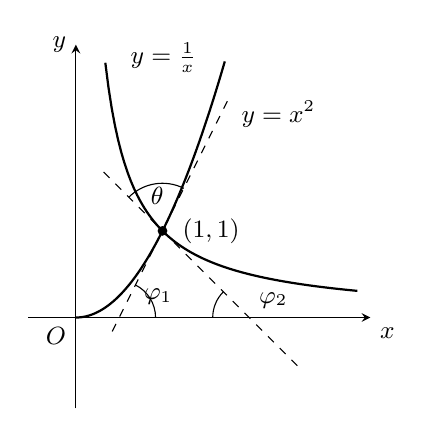
\begin{tikzpicture}[scale=1.1,>=stealth,font=\small]
  \draw[->] (-0.55,0) -- (3.40,0) node[below right] {$x$};
  \draw[->] (0,-1.05) -- (0,3.15) node[left] {$y$};
  \node[below left] at (0,0) {$O$};
  % y = x^2
  \draw[thick,domain=0:1.72,samples=60] plot (\x,{\x*\x});
  \node[right] at (1.80,2.35) {$y=x^2$};
  % y = 1/x
  \draw[thick,domain=0.34:3.25,samples=80] plot (\x,{1/\x});
  \node[right] at (0.52,3.00) {$y=\frac{1}{x}$};
  % 交点 (1,1)
  \fill (1,1) circle (1.6pt);
  \node[right] at (1.12,1.00) {$(1,1)$};
  % 切线 y=2x-1 (切于 y=x^2), 交 x 轴于 (0.5,0)
  \draw[dashed] (0.42,-0.16) -- (1.75,2.50);
  % 切线 y=-x+2 (切于 y=1/x), 交 x 轴于 (2,0)
  \draw[dashed] (0.32,1.68) -- (2.62,-0.62);
  % 夹角 theta (两切线之间)
  \draw (1,1) ++(63.4:0.55) arc (63.4:135:0.55);
  \node at (0.94,1.40) {$\theta$};
  % 角 phi_1 (y=x^2 的切线与 x 轴)
  \draw (0.5,0) ++(0.42,0) arc (0:63.4:0.42);
  \node at (0.95,0.24) {$\varphi_1$};
  % 角 phi_2 (y=1/x 的切线与 x 轴)
  \draw (2,0) ++(-0.42,0) arc (180:135:0.42);
  \node at (2.28,0.20) {$\varphi_2$};
\end{tikzpicture}
\caption{}\label{fig:3.1.2}
\end{figure}

\begin{example}\label{ex:3.1.15}
质点作直线运动, 它离原点 $O$ 的位移为 $x(t)$, 求质点运动的加速度(速度的变化率). 进而问: 在高度为 $h_0$ 处的物体作自由落体运动, 何时落到地面?
\end{example}

\begin{solution}
由例~\ref{ex:3.1.1} 知, (瞬时)速度 $v(t) = x'(t) = \lim\limits_{\Delta t\to0}\frac{x(t+\Delta t) - x(t)}{\Delta t}$, 它是质点位移 $x(t)$ 对时间 $t$ 的导数. 如果极限
\[
a(t) = v'(t) = \lim_{\Delta t\to0}\frac{v(t+\Delta t) - v(t)}{\Delta t} = \lim_{\Delta t\to0}\frac{x'(t+\Delta t) - x'(t)}{\Delta t} \xlongequal{\text{记作}} x''(t)
\]
存在且有限, 则称它为质点运动的加速度, 它是速度 $v(t)$ 对 $t$ 的导数, 也是位移 $x(t)$ 的 $2$ 阶导数.

自由落体运动, 其离地面高度 $h(t) = h_0 - \frac{1}{2}gt^2$, 速度 $v(t) = h'(t) = -gt$, 加速度 $a(t) = v'(t) = h''(t) = -g\ (\approx 980\,\text{cm/s}^2)$, 它是匀加速运动. 当 $t = \sqrt{\frac{2h_0}{g}}$ 时, 物体下落到地面.
\end{solution}

\begin{example}\label{ex:3.1.16}
汽车前灯的反光镜(或探照灯, 如图~\ref{fig:3.1.3} 所示)是由抛物线绕对称轴旋转而成的旋转抛物面. 这种反光镜就是利用抛物线的光学特性: 若光源置于抛物线的焦点上, 则光线经抛物线反射成一束平行于对称轴的光线(如图~\ref{fig:3.1.4} 所示). 试证之.
\end{example}

\begin{figure}[htbp]
\centering
\begin{minipage}[t]{0.45\textwidth}
\centering
\begin{tikzpicture}[scale=0.9,>=stealth]
  % 抛物面(旋转抛物面的轴截面)
  \draw[thick,domain=0.10:2.30,samples=80,smooth,variable=\t]
    plot ({0.18+1.67*((\t-1.20)/1.10)*((\t-1.20)/1.10)}, {\t});
  % 开口(椭圆, 后半虚线)
  \draw[thick] (1.85,2.30) arc (90:-90:0.30 and 1.10);
  \draw[dashed] (1.85,2.30) arc (90:270:0.30 and 1.10);
  % 焦点 F
  \draw[dashed] (0.62,1.20) circle (0.18);
  \fill (0.62,1.20) circle (1.4pt);
  \node[left,font=\small] at (0.42,1.20) {$F$};
  % 自焦点发出的光线经抛物面反射后平行于对称轴射出
  \foreach \y/\xb in {0.32/1.249,0.58/0.710,0.86/0.339,1.54/0.339,1.82/0.710,2.08/1.249}{
    \draw[->] (0.62,1.20) -- (\xb,\y);
    \draw[->] (\xb,\y) -- (2.75,\y);
  }
  \draw[->] (0.62,1.20) -- (2.75,1.20);
  \node[below,font=\small] at (1.45,-0.05) {探照灯};
\end{tikzpicture}
\caption{}\label{fig:3.1.3}
\end{minipage}
\hfill
\begin{minipage}[t]{0.45\textwidth}
\centering
\begin{tikzpicture}[scale=0.9,>=stealth]
  \draw[thick,domain=0.10:2.30,samples=80,smooth,variable=\t]
    plot ({0.18+1.67*((\t-1.20)/1.10)*((\t-1.20)/1.10)}, {\t});
  \draw[thick] (1.85,2.30) arc (90:-90:0.30 and 1.10);
  \draw[dashed] (1.85,2.30) arc (90:270:0.30 and 1.10);
  \draw[dashed] (0.62,1.20) circle (0.18);
  \fill (0.62,1.20) circle (1.4pt);
  \node[left,font=\small] at (0.42,1.20) {$F$};
  % 平行于对称轴的入射光线经抛物面反射后汇聚于焦点
  \foreach \y/\xb in {0.32/1.249,0.58/0.710,0.86/0.339,1.54/0.339,1.82/0.710,2.08/1.249}{
    \draw[->] (2.75,\y) -- (\xb,\y);
    \draw[->] (\xb,\y) -- (0.62,1.20);
  }
  \draw[->] (2.75,1.20) -- (0.62,1.20);
  \node[below,font=\small] at (1.45,-0.05) {太阳灶};
\end{tikzpicture}
\caption{}\label{fig:3.1.4}
\end{minipage}
\end{figure}

\begin{proof}
设抛物线的方程为 $y^2 = 2px$, 则焦点为 $F\left(\frac{p}{2}, 0\right)$. 在抛物线上任取一点 $A(x_0, y_0)$, 过 $A$ 点作切线 $L$, 记 $L$ 与线段 $AF$ 的夹角为 $\alpha$, $L$ 与 $x$ 轴的夹角为 $\beta$. 根据光学原理: 光线的入射角等于反射角. 因此, 如果能证明 $\alpha = \beta$, 则就证明了反射光线平行于 $x$ 轴(对称轴). 记 $L$ 与 $x$ 轴的交点为 $B$. 于是, $\alpha = \beta \iff AF = BF$.

将 $y^2 = 2px$ 两边关于 $x$ 求导得 $2yy' = 2p$, 所以, $y' = \frac{p}{y}$. 因此, 抛物线 $y^2 = 2px$ 在点 $A(x_0, y_0)$ 的切线 $L$ 的斜率为 $y'|_{x=x_0} = \frac{p}{y_0}$, 故 $L$ 的方程为
\[
y - y_0 = \frac{p}{y_0}(x - x_0).
\]
在上式中, 令 $y = 0$, 即得 $B$ 点坐标为 $(-x_0, 0)$. 因此,
\[
BF = \left|\frac{p}{2} + x_0\right|,
\]
\[
AF = \sqrt{\left(x_0 - \frac{p}{2}\right)^2 + y_0^2} = \sqrt{\left(x_0 - \frac{p}{2}\right)^2 + 2px_0} = \left|\frac{p}{2} + x_0\right| = BF.
\]
根据上述数学原理, 如果有一束平行于 $x$ 轴的光线经旋转抛物面反射到抛物线焦点 $F$(太阳灶就是由这原理造出来的, 以致在 $F$ 处达到高温, 如图~\ref{fig:3.1.5} 所示).
\end{proof}

\begin{figure}[htbp]
\centering
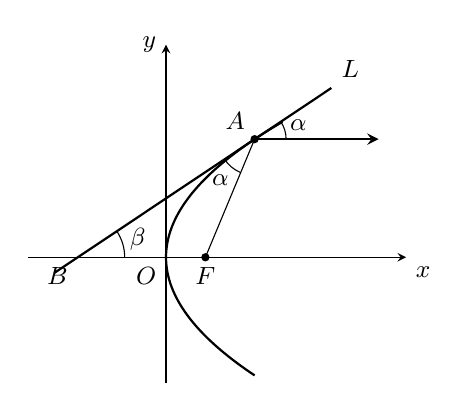
\begin{tikzpicture}[scale=1.0,>=stealth,font=\small]
  \draw[->] (-1.75,0) -- (3.05,0) node[below right] {$x$};
  \draw[->] (0,-1.60) -- (0,2.70) node[left] {$y$};
  \node[below left] at (0,0) {$O$};
  % 抛物线 y^2 = 2x  =>  x = y^2/2
  \draw[thick,domain=-1.50:1.72,samples=80,smooth,variable=\t] plot ({0.5*\t*\t},{\t});
  \coordinate (A) at (1.125,1.5);
  \coordinate (B) at (-1.125,0);
  \coordinate (F) at (0.5,0);
  % 切线 L (过 A, B)
  \draw[thick] (-1.42,-0.20) -- (2.10,2.15) node[above right] {$L$};
  % 反射光线 (平行于 x 轴)
  \draw[->,thick] (A) -- (2.70,1.5);
  % 焦半径 AF
  \draw (A) -- (F);
  \fill (A) circle (1.5pt);
  \node[above left] at (A) {$A$};
  \fill (F) circle (1.5pt);
  \node[below] at (F) {$F$};
  \node[below left] at (B) {$B$};
  % 角 beta (B 处: L 与 x 轴)
  \draw (B) ++(0.60,0) arc (0:33.7:0.60);
  \node at (-0.36,0.23) {$\beta$};
  % 角 alpha (A 处: L 与反射光线)
  \draw (A) ++(0.40,0) arc (0:33.7:0.40);
  \node at (1.68,1.68) {$\alpha$};
  % 角 alpha (A 处: L 与 AF)
  \draw (A) ++(213.7:0.46) arc (213.7:247.4:0.46);
  \node at (0.69,0.98) {$\alpha$};
\end{tikzpicture}
\caption{}\label{fig:3.1.5}
\end{figure}

\begin{exblock}{练习题 3.1}
  \item 设函数 $f$ 在点 $x_0$ 处可导, 则 $\lim\limits_{\Delta x\to0}\frac{f(x_0+\Delta x) - f(x_0-\Delta x)}{\Delta x} = 2f'(x_0)$. 举例说明: 即使上式左边的极限存在且有限, $f$ 在点 $x_0$ 处也未必可导.

  \item 在抛物线 $y = x^2$ 上哪些点的切线满足下面条件:
  \begin{enumerate}[label=(\arabic*)]
    \item 平行于直线 $y = 4x - 5$;
    \item 垂直于直线 $2x - 6y + 5 = 0$;
    \item 与直线 $3x - y + 1 = 0$ 交成 $45^\circ$ 的角.
  \end{enumerate}

  \item 证明: 抛物线 $y = x^2$ 上的两点 $(x_1, x_1^2)$ 与 $(x_2, x_2^2)$ 处的切线互相垂直的充分必要条件是 $x_1$ 与 $x_2$ 适合关系 $4x_1x_2 + 1 = 0$.

  \item 设 $f(x) = x(x-1)^2(x-2)^3$. 求 $f'(0)$, $f'(1)$, $f'(2)$.

  \item 设 $f(x_0) = 0$, $f'(x_0) = 4$. 求极限 $\lim\limits_{\Delta x\to0}\frac{f(x_0+\Delta x)}{\Delta x}$.

  \item 确定曲线 $y = \ln x$ 上哪些点的切线平行于下列直线: (1) $y = x - 1$; (2) $y = 2x - 3$.

  \item 求下列曲线在指定点 $P$ 的切线方程与法线方程:
  \begin{enumerate}[label=(\arabic*)]
    \item $y = \frac{x^2}{4}$, $P = (2,1)$;
    \item $y = \cos x$, $P = (0,1)$.
  \end{enumerate}

  \item 求下列函数的导函数:
  \begin{enumerate}[label=(\arabic*)]
    \item $f(x) = |x|^3$;
    \item $f(x) = \begin{cases}x+1, & x \geqslant 0,\\ 1, & x < 0.\end{cases}$
  \end{enumerate}

  \item 设 $f(x) = \begin{cases}x^2, & x \geqslant 3,\\ ax+b, & x < 3.\end{cases}$ 试确定 $a$, $b$ 的值, 使 $f$ 在 $x=3$ 处可导.

  \item 设 $g(0) = g'(0) = 0$, $f(x) = \begin{cases}g(x)\sin\frac{1}{x}, & x \neq 0,\\ 0, & x = 0.\end{cases}$ 求 $f'(0)$.

  \item 设函数 $f$ 在点 $x_0$ 处存在左右导数. 证明: $f$ 在点 $x_0$ 处连续.

  \item 设函数 $f$ 在 $[a,b]$ 上连续, 且 $f(a) = f(b) = K$, $f'_+(a)\cdot f'_-(b) > 0$. 证明: 在 $(a,b)$ 内至少有一点 $\xi$, 使 $f(\xi) = K$.

  \item 设 $f$ 在 $\mathbb{R}$ 上可导, 并且 $\lim\limits_{x\to\infty}f(x) = a \in \mathbb{R}$. 证明: 必 $\exists \xi \in \mathbb{R}$, s.t. $f'(\xi) = 0$.

  \item 设函数 $f$ 在 $x = a$ 处可导, 且 $f(a) \neq 0$. 求数列极限
  \[
  \lim_{n\to+\infty}\left(\frac{f\left(a+\frac{1}{n}\right)}{f(a)}\right)^n.
\]

  \item 设函数 $\varphi$ 在点 $a$ 处连续, 又在 $a$ 的近旁有 $f(x) = (x-a)\varphi(x)$ 和 $g(x) = |x-a|\varphi(x)$. 证明: $f$ 在点 $a$ 处可导, 并求 $f'(a)$. 问在什么条件下 $g$ 在点 $a$ 处可导.

  \item 求下列函数在指定点的导数:
  \begin{enumerate}[label=(\arabic*)]
    \item $f(x) = 3x^4 + 2x^3 + 5$, 求 $f'(0)$, $f'(1)$;
    \item $f(x) = \frac{x}{\cos x}$, 求 $f'(0)$, $f'(\pi)$;
    \item $f(x) = \sqrt{1 + \sqrt{x}}$, 求 $f'(0)$, $f'(1)$, $f'(4)$.
  \end{enumerate}

  \item 求下列函数的导数:
  \begin{enumerate}[label=(\arabic*)]
    \item $y = x^3 - 2x - 6$;
    \item $y = \sqrt{x} - \frac{1}{x}$;
    \item $y = \frac{1-x^2}{1+x+x^2}$;
    \item $y = \frac{x}{m} + \frac{m}{x} + 2\sqrt{x} + \frac{2}{\sqrt{x}}$;
    \item $y = x^3\log_3 x$;
    \item $y = \mathrm{e}^x\cos x$;
    \item $y = (x^2+1)(3x-1)(1-x^3)$;
    \item $y = \frac{\tan x}{x}$;
    \item $y = \frac{1+\ln x}{1-\ln x}$;
    \item $y = (\sqrt{x}+1)\arctan x$;
    \item $y = \frac{1+x^2}{\sin x + \cos x}$;
    \item $y = \mathrm{e}^{ax}\cos bx$;
    \item $y = \frac{\cos x - \sin x}{\cos x + \sin x}$;
    \item $y = x\sin x\ln x$;
    \item $y = \sqrt{x + \sqrt{x + \sqrt{x}}}$;
    \item $y = \ln(\cos x + \sin x)$;
    \item $y = (x^2-1)^3$;
    \item $y = \left(\frac{1+x^2}{1-x}\right)^3$;
    \item $y = \ln(\ln x)$;
    \item $y = \ln\frac{\sqrt{1+x} - \sqrt{1-x}}{\sqrt{1+x} + \sqrt{1-x}}$;
    \item $y = (\arctan x^3)^2$;
    \item $y = \arcsin(\sin^2 x)$;
    \item $y = \sin(\sin(\sin x))$;
    \item $y = \sin\left(\frac{x}{\sin\left(\frac{x}{\sin x}\right)}\right)$;
    \item $y = (x-a_1)^{a_1}(x-a_2)^{a_2}\cdots(x-a_n)^{a_n}$;
    \item $y = \sqrt[3]{\frac{(x+1)^2(x+2)^3}{(x+3)^4(x+4)^5}}$.
  \end{enumerate}

  \item 求下列函数的导数:
  \begin{enumerate}[label=(\arabic*)]
    \item $y = \frac{ax+b}{cx+d}$, 其中 $a, b, c, d$ 为常数;
    \item $y = \ln(x + \sqrt{x^2+a^2})$;
    \item $y = x^{x^x}$.
  \end{enumerate}

  \item 证明:
  \begin{enumerate}[label=(\arabic*)]
    \item $(\sinh x)' = \cosh x$;
    \item $(\cosh x)' = \sinh x$;
    \item $(\tanh x)' = \frac{1}{\cosh^2 x}$;
    \item $(\coth x)' = \frac{1}{\sinh^2 x}$.
  \end{enumerate}

  \item 以 $\operatorname{arsinh} x$, $\operatorname{arcosh} x$, $\operatorname{artanh} x$, $\operatorname{arcoth} x$ 分别表示各双曲函数的反函数. 试求下列函数的导数:
  \begin{enumerate}[label=(\arabic*)]
    \item $y = \operatorname{arsinh} x$;
    \item $y = \operatorname{arcosh} x$;
    \item $y = \operatorname{artanh} x$;
    \item $y = \operatorname{arcoth} x$.
  \end{enumerate}

  \item 设 $g$ 可导, $a$ 为实数. 对下列各函数计算 $f'(x)$, $f'(x+1)$, $f'(x-1)$:
  \begin{enumerate}[label=(\arabic*)]
    \item $f(x) = x^3$;
    \item $f(x) = g(x + g(x))$;
    \item $f(x) = g(x)g(a)$;
    \item $f(x) = g(x)g(x)$.
  \end{enumerate}

  \item 设 $f$ 为可导函数. 证明: 若 $x=1$ 时, 有 $\frac{\mathrm{d}}{\mathrm{d}x}f(x^2) = \frac{\mathrm{d}}{\mathrm{d}x}f^2(x)$, 且必有 $f'(1) = 0$ 或 $f(1) = 1$.

  \item 利用 $1 + x + \cdots + x^n$ 的和, 求出下列各式的和:
  \begin{enumerate}[label=(\arabic*)]
    \item $1 + 2x + 3x^2 + \cdots + nx^{n-1}$;
    \item $\sum\limits_{k=1}^{n}\frac{k}{2^{k-1}}$;
    \item $1^2 + 2^2 x + 3^2 x^2 + \cdots + n^2 x^{n-1}$.
  \end{enumerate}

  \item 设 $f$ 为可导函数, 求下列各函数的一阶导数:
  \begin{enumerate}[label=(\arabic*)]
    \item $y = f(\mathrm{e}^x)\mathrm{e}^{f(x)}$;
    \item $y = f(f(f(x)))$.
  \end{enumerate}

  \item 设 $\varphi$, $\psi$ 为可导函数, 求 $y'$:
  \begin{enumerate}[label=(\arabic*)]
    \item $y = \sqrt{\varphi^2(x) + \psi^2(x)}$;
    \item $y = \arctan\frac{\varphi(x)}{\psi(x)}$;
    \item $y = \log_{\varphi(x)}\psi(x)$ ($\varphi(x) > 0$, $\varphi(x) \neq 1$, $\psi(x) > 0$).
  \end{enumerate}

  \item 在曲线 $y = x^3$ 上取一点 $P$, 过 $P$ 的切线与该曲线交于 $Q$. 证明: 曲线在 $Q$ 点处的切线斜率正好是在 $P$ 点处切线斜率的 $4$ 倍.

  \item 设有一吊桥, 其铁链成抛物线型, 两端系于相距 $100$ m 高度相同的支柱上, 铁链的最低点在悬点下 $10$ m 处, 求铁链与支柱所成的角.

  \item 证明: 双曲线 $xy = a > 0$ 在各点处的切线与两坐标轴所围成的三角形的面积为常数.

  \item 有一底半径为 $R$ cm, 高为 $h$ cm 的正圆锥容器, 顶点有一小孔, 以便向容器内注水. 今以 $A\ \text{cm}^3/\text{s}$ 的速度向容器内注水, 试求容器内水位等于锥高一半时, 水面上升的速度.

  \item 水自高为 $18$ cm、底半径为 $6$ cm 的圆锥形漏斗流入直径为 $10$ cm 的圆柱形桶内. 已知漏斗水深 $12$ cm 时水面下降速度为 $1$ cm/s, 求此时桶中水面上升的速度.
\end{exblock}

\begin{exblock}{思考题 3.1}
  \item 证明: Riemann 函数 $R(x)$ 处处不可导.

  \item 构造一个可导函数 $f$, 使 $f$ 在有理点处取有理数值, 它的导函数在有理点处取无理数值.

  \item
  \begin{enumerate}[label=(\arabic*)]
    \item 构造一个连续函数, 它仅在已知点 $a_1, \cdots, a_n$ 处不可导;
    \item 构造一个函数, 它仅在点 $a_1, \cdots, a_n$ 处可导.
  \end{enumerate}

  \item 设 $f$ 为三次多项式, 且 $f(a) = f(b) = 0$. 证明: 函数 $f$ 在 $[a,b]$ 上不变号的必要充分条件是 $f'(a)f'(b) \leqslant 0$.

  \item 证明组合恒等式:
  \begin{enumerate}[label=(\arabic*)]
    \item $\sum\limits_{k=1}^{n}kC_n^k = n2^{n-1}$, $n \in \mathbb{N}$;
    \item $\sum\limits_{k=1}^{n}k^2C_n^k = n(n+1)2^{n-2}$, $n \in \mathbb{N}$.
  \end{enumerate}
  (提示: 分别对 $(1+x)^n = \sum\limits_{k=0}^{n}C_n^k x^k$ 与 $nx(1+x)^{n-1} = \sum\limits_{k=1}^{n}kC_n^k x^{k-1}$ 两边关于 $x$ 求导.)

  \item 设 $f(0) = 0$, $f'(0)$ 存在且有限, 令 $x_n = f\left(\frac{1}{n^2}\right) + f\left(\frac{2}{n^2}\right) + \cdots + f\left(\frac{n}{n^2}\right)$. 证明: $\lim\limits_{n\to+\infty}x_n = \frac{f'(0)}{2}$. 并利用以上结果计算:
  \begin{enumerate}[label=(\arabic*)]
    \item $\lim\limits_{n\to+\infty}\sum\limits_{k=1}^{n}\sin\frac{k}{n^2}$;
    \item $\lim\limits_{n\to+\infty}\prod\limits_{k=1}^{n}\left(1 + \frac{k}{n^2}\right)$, 其中 $\prod\limits_{k=1}^{n}$ 表示 $n$ 个数连乘.
  \end{enumerate}

  \item 设函数 $f$ 在 $x=0$ 处连续, 如果 $\lim\limits_{x\to0}\frac{f(2x) - f(x)}{x} = m$, 证明: $f'(0) = m$.

  \item 在区间 $[-1,1]$ 上讨论二次函数 $f(x) = ax^2 + bx + c$, 如果 $|f(x)| \leqslant 1$, $\forall x \in [-1,1]$, 证明: $|f'(x)| \leqslant 4$, $\forall x \in [-1,1]$.

  \item (1) 设 $f_n$, $f$ 为 $\mathbb{R}$ 上的一元函数, $f_n$ 在 $\mathbb{R}$ 上连续, $n = 1, 2, \cdots$, 且 $\lim\limits_{n\to+\infty}f_n(x) = f(x)$, $x \in \mathbb{R}$. 证明: 存在 $(\alpha,\beta) \subset \mathbb{R}$, 使得 $f$ 在 $(\alpha,\beta)$ 上是有界的.
  (2) 设 $g$ 在 $\mathbb{R}$ 上可导. 证明: 存在 $(\alpha,\beta) \subset \mathbb{R}$, 使得 $g'$ 在 $(\alpha,\beta)$ 上有界.
  (3) 使得导函数 $g'$ 在任何开区间 $(\alpha,\beta) \subset \mathbb{R}$ 上都无界的函数 $g$ 是不存在的.

  \item 在 $[0,1]$ 上适合条件 $|P| \leqslant 1$ 的二次多项式 $P$ 的全体记为 $V$, 求 $\sup\{|P'(0)|\}$.
\end{exblock}

% ====================================================================
%  徐森林、薛春华《数学分析》（第一册）
%  \S3.2  高阶导数、参变量函数的导数、导数的 Leibniz 公式
%  源：原书印刷页 171-185（PDF 物理页 177-191）
%  底本：PaddleOCR-VL-1.6 + 高清影印比对校订
%  规范：全西文半角标点；单一落盘出口 _texout.py
% ====================================================================
\section{高阶导数、参变量函数的导数、导数的 Leibniz 公式}\label{sec:3.2}

例~\ref{ex:3.1.15} 指出, 加速度就是位移对时间 $t$ 的 2 阶导数. 自然会想到要进一步研究高阶导数.

\begin{definition}\label{def:3.2.1}
如果 $f$ 的导函数 $f'$ 在点 $x_0$ 处可导, 则称 $f'$ 在点 $x_0$ 处的导数为 $f$ 在点 $x_0$ 的 2 阶导数, 记作
\[
f''(x_0) = \lim_{x\to x_0}\frac{f'(x) - f'(x_0)}{x - x_0} = \lim_{\Delta x\to0}\frac{f'(x_0+\Delta x) - f'(x_0)}{\Delta x}.
\]
同时称 $f$ 在点 $x_0$ 处 2 阶可导. 2 阶导数也可记为 $\left.\frac{\mathrm{d}^{2}f}{\mathrm{d}x^{2}}\right|_{x=x_0}$, $\left.\frac{\mathrm{d}^{2}y}{\mathrm{d}x^{2}}\right|_{x=x_0}$.

类似可定义 3 阶, 4 阶, $\cdots$, $n$ 阶导数:
\[
\begin{aligned}
f^{(n)}(x_0) &= \lim_{x\to x_0}\frac{f^{(n-1)}(x) - f^{(n-1)}(x_0)}{x - x_0}\\
&= \lim_{\Delta x\to0}\frac{f^{(n-1)}(x_0+\Delta x) - f^{(n-1)}(x_0)}{\Delta x},
\end{aligned}
\]
$f'' = (f')'$, $f^{(4)} = (f''')'$, $\cdots$, $f^{(n)} = (f^{(n-1)})'$. $n$ 阶导数也可记为 $\left.\frac{\mathrm{d}^{n}f}{\mathrm{d}x^{n}}\right|_{x=x_0}$, $\left.\frac{\mathrm{d}^{n}y}{\mathrm{d}x^{n}}\right|_{x=x_0}$.

$f$ 在开区间 $(a,b)$ 的每一点处 $n$ 阶可导, 则称 $f$ 在 $(a,b)$ 上 $n$ 阶可导.
\end{definition}

由 $n$ 阶导数定义, 显然有
\[
(f \pm g)^{(n)} = f^{(n)} \pm g^{(n)},\quad (\lambda f)^{(n)} = \lambda f^{(n)},\ \lambda \in \mathbb{R}.
\]

\begin{theorem}[Leibniz]\label{thm:3.2.1}
设 $f$ 与 $g$ 在区间 $I$ 上都 $n$ 阶可导, 则
\[
(fg)^{(n)} = \sum_{k=0}^{n}\mathrm{C}_{n}^{k}f^{(n-k)}g^{(k)},
\]
其中, $\mathrm{C}_{n}^{k} = \frac{n!}{k!(n-k)!}$ 为组合数, $g^{(0)} = g$, $f^{(0)} = f$.
\end{theorem}

\begin{proof}
用归纳法. 当 $n = 1$ 时,
\[
(fg)' = f'g + fg' = \sum_{k=0}^{1}\mathrm{C}_{1}^{k}f^{(1-k)}g^{(k)}.
\]
假设 $n = l$ 时, 有
\[
(fg)^{(l)} = \sum_{k=0}^{l}\mathrm{C}_{l}^{k}f^{(l-k)}g^{(k)}.
\]
那么, 当 $n = l+1$ 时, 有
\[
\begin{aligned}
(fg)^{(l+1)} &= ((fg)^{(l)})' = \left(\sum_{k=0}^{l}\mathrm{C}_{l}^{k}f^{(l-k)}g^{(k)}\right)'\\
&= \sum_{k=0}^{l}\mathrm{C}_{l}^{k}\left[(f^{(l-k)})'g^{(k)} + f^{(l-k)}(g^{(k)})'\right]\\
&= \sum_{k=0}^{l}\mathrm{C}_{l}^{k}\left[f^{(l+1-k)}g^{(k)} + f^{(l-k)}g^{(k+1)}\right]\\
&= \mathrm{C}_{l}^{0}f^{(l+1)}g + \sum_{k=1}^{l}\mathrm{C}_{l}^{k}f^{(l+1-k)}g^{(k)} + \sum_{k=0}^{l-1}\mathrm{C}_{l}^{k}f^{(l-k)}g^{(k+1)} + \mathrm{C}_{l}^{l}fg^{(l+1)}\\
&= \mathrm{C}_{l+1}^{0}f^{(l+1)}g + \sum_{k=1}^{l}(\mathrm{C}_{l}^{k} + \mathrm{C}_{l}^{k-1})f^{(l+1-k)}g^{(k)} + \mathrm{C}_{l+1}^{l+1}fg^{(l+1)}\\
&= \sum_{k=0}^{l+1}\mathrm{C}_{l+1}^{k}f^{(l+1-k)}g^{(k)}.
\end{aligned}
\]
\end{proof}

\begin{example}\label{ex:3.2.1}
求 $y = x^{n}$ 的各阶导函数, $n \in \mathbb{N}$.
\end{example}

\begin{solution}
\[
\begin{aligned}
y' &= nx^{n-1},\\
y'' &= n(n-1)x^{n-2},\\
&\cdots\\
y^{(n-1)} &= n(n-1)\cdots2x,\\
y^{(n)} &= n!,\\
y^{(n+1)} &= y^{(n+2)} = \cdots = 0.
\end{aligned}
\]
\end{solution}

\begin{example}\label{ex:3.2.2}
求下列函数的各阶导函数:
(1) $y = a^{x}$ ($a > 0$), 特别地, $y = \mathrm{e}^{x}$; (2) $y = \mathrm{e}^{ax}$;
(3) $y = \sin x$; (4) $y = \cos x$; (5) $y = \frac{1}{x-a}$; (6) $y = \frac{1}{x^{2}-3x+2}$.
\end{example}

\begin{solution}
(1) $y' = a^{x}\ln a$, $\cdots$, $y^{(n)} = a^{x}(\ln a)^{n}$. 特别地, $\left(\mathrm{e}^{x}\right)^{(n)} = \mathrm{e}^{x}$.

(2) $y' = a\mathrm{e}^{ax}$, $\cdots$, $y^{(n)} = a^{n}\mathrm{e}^{ax}$.

(3) $y' = \cos x = \sin\left(x + \frac{\pi}{2}\right)$. 设 $y^{(k)} = \sin\left(x + \frac{k\pi}{2}\right)$, 则有
\[
y^{(k+1)} = (y^{(k)})' = \cos\left(x + \frac{k\pi}{2}\right)\cdot1 = \sin\left[x + \frac{(k+1)\pi}{2}\right].
\]
于是, $\forall n \in \mathbb{N}$, 有
\[
y^{(n)} = \sin\left(x + \frac{n\pi}{2}\right).
\]

(4) 类似 (3), 可证 $(\cos x)^{(n)} = \cos\left(x + \frac{n\pi}{2}\right)$, $n \in \mathbb{N}$. 或者
\[
\begin{aligned}
(\cos x)^{(n)} &= \left(\sin\left(x + \frac{\pi}{2}\right)\right)^{(n)} = \sin\left(x + \frac{\pi}{2} + \frac{n\pi}{2}\right)\\
&= \cos\left(x + \frac{n\pi}{2}\right).
\end{aligned}
\]

(5) $y = \frac{1}{x-a} = (x-a)^{-1}$,
\[
y' = -(x-a)^{-2},\quad y'' = 2(x-a)^{-3},\quad \cdots,
\]
\[
y^{(n)} = (-1)^{n}\cdot n!(x-a)^{-(n+1)} = \frac{(-1)^{n}\cdot n!}{(x-a)^{(n+1)}}.
\]

(6)
\[
\begin{aligned}
y &= \frac{1}{x^{2}-3x+2} = \frac{1}{x-2} - \frac{1}{x-1},\\
y^{(n)} &= \left(\frac{1}{x-2}\right)^{(n)} - \left(\frac{1}{x-1}\right)^{(n)} = \frac{(-1)^{n}n!}{(x-2)^{n+1}} - \frac{(-1)^{n}n!}{(x-1)^{n+1}}\\
&= (-1)^{n}n!\left[\frac{1}{(x-2)^{n+1}} - \frac{1}{(x-1)^{n+1}}\right].
\end{aligned}
\]
\end{solution}

\begin{example}\label{ex:3.2.3}
设 $f(x) = a_{n}(x-x_0)^{n} + a_{n-1}(x-x_0)^{n-1} + \cdots + a_{1}(x-x_0) + a_{0}$ 为 $n$ 次多项式, 其中 $a_{n} \neq 0$,
\[
a_{k} = \frac{f^{(k)}(x_0)}{k!},\quad k = 0, 1, \cdots, n,
\]
因此,
\[
f(x) = \sum_{k=0}^{n}a_{k}(x-x_0)^{k} = \sum_{k=0}^{n}\frac{f^{(k)}(x_0)}{k!}(x-x_0)^{k}.
\]
\end{example}

\begin{proof}
因为
\[
\begin{aligned}
f(x) &= \sum_{k=0}^{n}a_{k}(x-x_0)^{k},\\
f'(x) &= \sum_{k=1}^{n}ka_{k}(x-x_0)^{k-1},\\
&\cdots\\
f^{(l)}(x) &= \sum_{k=l}^{n}k(k-1)\cdots(k-l+1)a_{k}(x-x_0)^{k-l},\\
&\cdots\\
f^{(n)}(x) &= n!a_{n},
\end{aligned}
\]
所以, $f(x_0) = a_0$, $f'(x_0) = a_1$, $\cdots$, $f^{(l)}(x_0) = l!a_l$, $\cdots$, $f^{(n)}(x_0) = n!a_n$, 即
\[
a_{l} = \frac{f^{(l)}(x_0)}{l!},\quad l = 0, 1, \cdots, n.
\]
\end{proof}

\begin{example}\label{ex:3.2.4}
设 $y = \mathrm{e}^{x}\cos x$, 求 $y^{(n)}$, $y^{(5)}$.
\end{example}

\begin{solution}
因为 $(\mathrm{e}^{x})^{(k)} = \mathrm{e}^{x}$, $(\cos x)^{(k)} = \cos\left(x + \frac{k\pi}{2}\right)$, 故由 Leibniz 求导公式知
\[
\begin{aligned}
y^{(n)} &= \left(\mathrm{e}^{x}\cos x\right)^{(n)} = \sum_{k=0}^{n}\mathrm{C}_{n}^{k}\left(\mathrm{e}^{x}\right)^{(n-k)}\left(\cos x\right)^{(k)}\\
&= \sum_{k=0}^{n}\mathrm{C}_{n}^{k}\mathrm{e}^{x}\cos\left(x + \frac{k\pi}{2}\right),
\end{aligned}
\]
当 $n = 5$ 时,
\[
\begin{aligned}
y^{(5)} &= \sum_{k=0}^{5}\mathrm{C}_{5}^{k}\mathrm{e}^{x}\cos\left(x + \frac{k\pi}{2}\right)\\
&= \mathrm{e}^{x}\left[\cos x + 5\cos\left(x + \frac{\pi}{2}\right) + 10\cos\left(x + \frac{2\pi}{2}\right) + 10\cos\left(x + \frac{3\pi}{2}\right)\right.\\
&\quad \left. + 5\cos\left(x + \frac{4\pi}{2}\right) + \cos\left(x + \frac{5\pi}{2}\right)\right]\\
&= \mathrm{e}^{x}(\cos x - 5\sin x - 10\cos x + 10\sin x + 5\cos x - \sin x)\\
&= 4\mathrm{e}^{x}(\sin x - \cos x).
\end{aligned}
\]
\end{solution}

\begin{example}\label{ex:3.2.5}
设 $y = x^{2}\cos x$, 求 $y^{(50)}$.
\end{example}

\begin{solution}
由 Leibniz 求导公式知,
\[
\begin{aligned}
y^{(50)} &= \sum_{k=0}^{50}\mathrm{C}_{50}^{k}\left(\cos x\right)^{(50-k)}\left(x^{2}\right)^{(k)}\\
&= x^{2}\left(\cos x\right)^{(50)} + \mathrm{C}_{50}^{1}\cdot2x\left(\cos x\right)^{(49)} + \mathrm{C}_{50}^{2}\cdot2\left(\cos x\right)^{(48)}\\
&= x^{2}\cos\left(x + \frac{50\pi}{2}\right) + 100x\cos\left(x + \frac{49\pi}{2}\right) + 2450\cos\left(x + \frac{48\pi}{2}\right)\\
&= -x^{2}\cos x - 100x\sin x + 2450\cos x\\
&= (2450 - x^{2})\cos x - 100x\sin x.
\end{aligned}
\]
\end{solution}

\begin{example}\label{ex:3.2.6}
设
\[
f(x) = \begin{cases}x^{4}\sin\frac{1}{x}, & x \neq 0,\\ 0, & x = 0,\end{cases}
\]
求 $f''(x)$.
\end{example}

\begin{solution}
由
\[
f'(0) = \lim_{x\to0}\frac{f(x) - f(0)}{x - 0} = \lim_{x\to0}\frac{x^{4}\sin\frac{1}{x} - 0}{x - 0} = \lim_{x\to0}x^{3}\sin\frac{1}{x} = 0,
\]
得到
\[
f'(x) = \begin{cases}4x^{3}\sin\frac{1}{x} - x^{2}\cos\frac{1}{x}, & x \neq 0,\\ 0, & x = 0.\end{cases}
\]
按照 2 阶导数定义, 有
\[
\begin{aligned}
f''(0) &= \lim_{x\to0}\frac{f'(x) - f'(0)}{x - 0} = \lim_{x\to0}\frac{4x^{3}\sin\frac{1}{x} - x^{2}\cos\frac{1}{x} - 0}{x - 0}\\
&= \lim_{x\to0}\left(4x^{2}\sin\frac{1}{x} - x\cos\frac{1}{x}\right) = 0,
\end{aligned}
\]
从而
\[
\begin{aligned}
f''(x) &= \begin{cases}12x^{2}\sin\frac{1}{x} - 4x\cos\frac{1}{x} - 2x\cos\frac{1}{x} - \sin\frac{1}{x}, & x \neq 0,\\ 0, & x = 0\end{cases}\\
&= \begin{cases}(12x^{2} - 1)\sin\frac{1}{x} - 6x\cos\frac{1}{x}, & x \neq 0,\\ 0, & x = 0.\end{cases}
\end{aligned}
\]
进一步, 由于极限
\[
\lim_{x\to0}\frac{(12x^{2} - 1)\sin\frac{1}{x} - 6x\cos\frac{1}{x} - 0}{x - 0} = \lim_{x\to0}\left[12x\sin\frac{1}{x} - \frac{\sin\frac{1}{x} + 6x\cos\frac{1}{x}}{x}\right]
\]
不存在, 故 $\forall n \in \mathbb{N}$, $f^{(n)}(x)$ 对 $x \neq 0$ 都是存在的, 但是 $f'''(0)$ 已不存在.
\end{solution}

\begin{definition}\label{def:3.2.2}
设函数 $f$ 在 $U \subsetneq \mathbb{R}$ 上连续, 则称 $f$ 在 $U$ 上是 $C^{0}$ 的, 记 $U$ 上 $C^{0}$ 函数的全体为 $C^{0}(U, \mathbb{R})$; 设 $r \in \mathbb{N}$, 如果 $f$ 在开集 $U \subsetneq \mathbb{R}$ 上 $r$ 阶连续可导, 则称 $f$ 在 $U$ 上是 $C^{r}$ 的, 记 $U$ 上 $C^{r}$ 函数的全体为 $C^{r}(U, \mathbb{R})$; 如果 $f$ 在开集 $U \subsetneq \mathbb{R}$ 上各阶连续可导, 则称 $f$ 在 $U$ 上是 $C^{\infty}$ 的, 记 $U$ 上 $C^{\infty}$ 函数的全体为 $C^{\infty}(U, \mathbb{R})$; 如果 $f$ 在开集 $U \subsetneq \mathbb{R}$ 上, 每一点 $x_0 \in U$ 的邻近可展开为收敛的幂级数
\[
f(x) = \sum_{n=0}^{\infty}a_{n}(x-x_0)^{n},\quad x \in (x_0 - \delta_{x_0}, x_0 + \delta_{x_0}) \subset U,
\]
则称 $f$ 在 $U$ 上是 $C^{\omega}$ 的或实解析的. 第 3 册将证明 $a_{n} = \frac{f^{(n)}(x_0)}{n!}$, 称为 $f$ 的 Taylor 系数.

记 $U$ 上 $C^{\omega}$ 函数的全体为 $C^{\omega}(U, \mathbb{R})$.
\end{definition}

\begin{example}\label{ex:3.2.7}
(1) 设 $r = 0, 1, 2, \cdots$, 则
\[
f(x) = \begin{cases}x^{2r+1}\sin\frac{1}{x}, & x \neq 0,\\ 0, & x = 0\end{cases}
\]
在 $\mathbb{R}$ 上是 $C^{r}$ 的, 但非 $C^{r+1}$ 的;

(2) $f(x) = \begin{cases}\mathrm{e}^{-\frac{1}{x}}, & x > 0,\\ 0, & x \leqslant 0\end{cases}$ 为 $C^{\infty}$ 的但非 $C^{\omega}$ 的函数.
\end{example}

\begin{proof}
(1) 容易看出, 当 $r = 0$ 时,
\[
f(x) = \begin{cases}x\sin\frac{1}{x}, & x \neq 0,\\ 0, & x = 0\end{cases}
\]
是 $C^{0}$ 的但非 $C^{1}$ 的函数.

当 $r = 1, 2, \cdots$ 时,
\[
\begin{aligned}
f'(0) &= \lim_{x\to0}\frac{f(x) - f(0)}{x - 0} = \lim_{x\to0}\frac{x^{2r+1}\sin\frac{1}{x} - 0}{x - 0}\\
&= \lim_{x\to0}x^{2r}\sin\frac{1}{x} = 0,
\end{aligned}
\]
\[
f'(x) = \begin{cases}(2r+1)x^{2r}\sin\frac{1}{x} - x^{2r-1}\cos\frac{1}{x}, & x \neq 0,\\ 0, & x = 0,\end{cases}
\]
\[
f''(x) = \begin{cases}x^{2r-2}(\cdots) - x^{2r-3}\sin\frac{1}{x}, & x \neq 0,\\ 0, & x = 0,\end{cases}
\]
\[
\cdots
\]
\[
f^{(r)}(x) = \begin{cases}x^{2}(\cdots) \pm x\sin\frac{1}{x}\left(\text{或}\ \pm x\cos\frac{1}{x}\right), & x \neq 0,\\ 0, & x = 0.\end{cases}
\]
\[
\begin{aligned}
f^{(r+1)}(0) &= \lim_{x\to0}\frac{f^{(r)}(x) - f^{(r)}(0)}{x - 0}\\
&= \lim_{x\to0}\left\{x(\cdots) \pm \sin\frac{1}{x}\left(\text{或}\ \pm\cos\frac{1}{x}\right)\right\}
\end{aligned}
\]
不存在. 综上可知, $f$ 是 $C^{r}$ 的但非 $C^{r+1}$ 的.

(2) 我们应用归纳法证明
\[
f^{(n)}(x) = \begin{cases}p_{n}\left(\frac{1}{x}\right)\mathrm{e}^{-\frac{1}{x}}, & x > 0,\\ 0, & x \leqslant 0,\end{cases}
\]
其中 $p_{n}(u)$ 为 $u$ 的多项式.

事实上, 当 $n = 1$ 时,
\[
f'_{-}(0) = \lim_{x\to0^{-}}\frac{f(x) - f(0)}{x - 0} = \lim_{x\to0^{-}}\frac{0 - 0}{x - 0} = \lim_{x\to0^{-}}0 = 0,
\]
\[
\begin{aligned}
f'_{+}(0) &= \lim_{x\to0^{+}}\frac{f(x) - f(0)}{x - 0} = \lim_{x\to0^{+}}\frac{\mathrm{e}^{-\frac{1}{x}} - 0}{x - 0}\\
&= \lim_{u\to+\infty}\frac{u}{\mathrm{e}^{u}} \xlongequal{\text{例~\ref{ex:2.2.14}(2)}} 0,
\end{aligned}
\]
\[
f'(0) = f'_{-}(0) = f'_{+}(0) = 0,
\]
\[
f'(x) = \begin{cases}\frac{1}{x^{2}}\mathrm{e}^{-\frac{1}{x}}, & x > 0,\\ 0, & x \leqslant 0\end{cases}
= \begin{cases}p_{1}\left(\frac{1}{x}\right)\mathrm{e}^{-\frac{1}{x}}, & x > 0,\\ 0, & x \leqslant 0.\end{cases}
\]
假设 $n = k$ 时, 有
\[
f^{(k)}(x) = \begin{cases}p_{k}\left(\frac{1}{x}\right)\mathrm{e}^{-\frac{1}{x}}, & x > 0,\\ 0, & x \leqslant 0,\end{cases}
\]
则当 $n = k+1$ 时,
\[
f^{(k+1)}_{-}(0) = \lim_{x\to0^{-}}\frac{f^{(k)}(x) - f^{(k)}(0)}{x - 0} = \lim_{x\to0^{-}}\frac{0 - 0}{x - 0} = \lim_{x\to0^{-}}0 = 0,
\]
\[
\begin{aligned}
f^{(k+1)}_{+}(0) &= \lim_{x\to0^{+}}\frac{f^{(k)}(x) - f^{(k)}(0)}{x - 0} = \lim_{x\to0^{+}}\frac{p_{k}\left(\frac{1}{x}\right)\mathrm{e}^{-\frac{1}{x}} - 0}{x - 0}\\
&= \lim_{u\to+\infty}\frac{up_{k}(u)}{\mathrm{e}^{u}} \xlongequal{\text{例~\ref{ex:2.2.14}(2)}} 0,
\end{aligned}
\]
\[
\begin{aligned}
f^{(k+1)}(x) &= \begin{cases}p'_{k}\left(\frac{1}{x}\right)\cdot\frac{-1}{x^{2}}\mathrm{e}^{-\frac{1}{x}} + p_{k}\left(\frac{1}{x}\right)\cdot\frac{1}{x^{2}}\mathrm{e}^{-\frac{1}{x}}, & x > 0,\\ 0, & x \leqslant 0\end{cases}\\
&= \begin{cases}p_{k+1}\left(\frac{1}{x}\right)\mathrm{e}^{-\frac{1}{x}}, & x > 0,\\ 0, & x \leqslant 0.\end{cases}
\end{aligned}
\]
因为 $f$ 有 $r+1$ 阶导函数 $f^{(r+1)}(x)$, 所以根据定理~\ref{thm:3.1.2} 推得 $f^{(r)}(x)$ 在 $\mathbb{R}$ 上连续. 于是, $f$ 为 $C^{\infty}$ 函数, 但它不是 $C^{\omega}$ 函数. 利用反证法假设 $f$ 为 $C^{\omega}$ 函数, 则 $\exists \delta > 0$, s.t.
\[
f(x) = \sum_{n=0}^{\infty}\frac{f^{(n)}(0)}{n!}x^{n} = \sum_{n=0}^{\infty}\frac{0}{n!}x^{n} = 0,\quad x \in (-\delta, \delta),
\]
这与 $f(x) = \mathrm{e}^{-\frac{1}{x}} \neq 0$, $x \in (0, \delta)$ 矛盾.
\end{proof}

\begin{remark}\label{rem:3.2.1}
例~\ref{ex:3.2.7}(2) 是近代数学中单位分解所用到的最重要的数学分析典型实例.
\end{remark}

\begin{example}\label{ex:3.2.8}
(1) 设 $f(x) = \arcsin x$, 则
\[
f^{(n)}(0) = \begin{cases}0, & n = 2k,\\ [(2k-1)!!]^{2}, & n = 2k+1;\end{cases}
\]

(2) 设 $f(x) = (\arcsin x)^{2}$, 则
\[
f^{(n)}(0) = \begin{cases}0, & n = 2k+1,\\ 2^{2k+1}(k!)^{2}, & n = 2k+2.\end{cases}
\]
\end{example}

\begin{proof}
(1)
\[
f(x) = \arcsin x,
\]
\[
f'(x) = \frac{1}{\sqrt{1-x^{2}}},\quad f''(x) = \frac{x}{(1-x^{2})^{3/2}},
\]
\[
(1-x^{2})f''(x) = xf'(x).
\]
将上式两边求 $n$ 阶导数并应用 Leibniz 求导公式得到
\[
\begin{aligned}
&(1-x^{2})f^{(n+2)}(x) - 2nxf^{(n+1)}(x) - n(n-1)f^{(n)}(x)\\
=&\ xf^{(n+1)}(x) + nf^{(n)}(x).
\end{aligned}
\]
令 $x = 0$, 代入上式得
\[
f^{(n+2)}(0) = n(n-1)f^{(n)}(0) + nf^{(n)}(0) = n^{2}f^{(n)}(0).
\]
由此知,
\[
\begin{aligned}
f^{(2k)}(0) &= (2k-2)^{2}f^{(2k-2)}(0) = 4(k-1)^{2}f^{(2k-2)}(0)\\
&= \cdots = 4^{k-1}[(k-1)!]^{2}f''(0) = 0,
\end{aligned}
\]
\[
\begin{aligned}
f^{(2k+1)}(0) &= (2k-1)^{2}f^{(2k-1)}(0)\\
&= (2k-1)^{2}(2k-3)^{2}f^{(2k-3)}(0)\\
&= (2k-1)^{2}(2k-3)^{2}\cdots3^{2}\cdot1^{2}f'(0)\\
&= [(2k-1)!!]^{2},
\end{aligned}
\]
\[
f^{(n)}(0) = \begin{cases}0, & n = 2k,\\ [(2k-1)!!]^{2}, & n = 2k+1.\end{cases}
\]

(2) 由 $f(x) = (\arcsin x)^{2}$, 得
\[
f'(x) = \frac{2\arcsin x}{\sqrt{1-x^{2}}},\quad (1-x^{2})f'^{2}(x) = 4f(x).
\]
两边对 $x$ 求导得
\[
2(1-x^{2})f'(x)f''(x) - 2xf'^{2}(x) = 4f'(x).
\]
当 $f'(x) \neq 0 \iff x \neq 0$ 时, 整理得
\[
(1-x^{2})f''(x) - xf'(x) = 2.
\]
在上式两边令 $x \to 0$, 推出当 $x = 0$ 时, 上式也成立.

再对上面等式关于 $x$ 求 $n$ 阶导数, 并应用 Leibniz 求导公式得
\[
\begin{aligned}
&(1-x^{2})f^{(n+2)}(x) - 2nxf^{(n+1)}(x) - n(n-1)f^{(n)}(x)\\
&- xf^{(n+1)}(x) - nf^{(n)}(x) = 0.
\end{aligned}
\]
令 $x = 0$, 代入上式得到
\[
f^{(n+2)}(0) = n^{2}f^{(n)}(0).
\]
由 $f'(0) = 0$, $f''(0) = 2$ 推出
\[
f^{(2k+1)}(0) = 0,
\]
\[
f^{(2k+2)}(0) = (2k)^{2}(2k-2)^{2}\cdots2^{2}f''(0) = 2^{2k+1}(k!)^{2}.
\]
\end{proof}

现在来研究参变量函数的导数. 设平面曲线的一般表达式为参数方程: $(x, y) = (x(t), y(t))$, $t \in (\alpha, \beta)$ 为参数.

曲线 $L$ 上点 $P = (x(t_0), y(t_0))$ 为定点, $Q = (x(t), y(t)) = (x(t_0+\Delta t), y(t_0+\Delta t))$ 为动点. 如果 $x(t)$, $y(t)$ 在 $t = t_0$ 处可导, 且 $x'(t_0) \neq 0$, 则割线 $PQ$ 的斜率为
\[
\frac{\Delta y}{\Delta x} = \frac{y(t) - y(t_0)}{x(t) - x(t_0)} = \frac{y(t_0+\Delta t) - y(t_0)}{x(t_0+\Delta t) - x(t_0)}.
\]
$P$ 点处切线(割线 $PQ$ 当 $\Delta t \to 0$, $\Delta x \to 0$, $Q \to P$ 时的极限位置)的斜率为
\[
\tan\alpha = \lim_{\Delta x\to0}\frac{\Delta y}{\Delta x} = \lim_{\Delta t\to0}\frac{\frac{y(t_0+\Delta t) - y(t_0)}{\Delta t}}{\frac{x(t_0+\Delta t) - x(t_0)}{\Delta t}} = \frac{y'(t_0)}{x'(t_0)}.
\]
如果 $x(t)$, $y(t)$ 都是 $[\alpha, \beta]$ 上的 $C^{r}$ 函数 ($r \geqslant 1$), 且 $x'^{2}(t) + y'^{2}(t) \neq 0$, 则称 $L$ 为 $C^{r}$ 的光滑正则曲线. 此时, 不仅每一点处都有切线, 且切线与 $x$ 轴正向的夹角 $\alpha(t)$ 为 $t$ 的连续函数(如图~\ref{fig:3.2.1} 所示).

\begin{figure}[htbp]
\centering
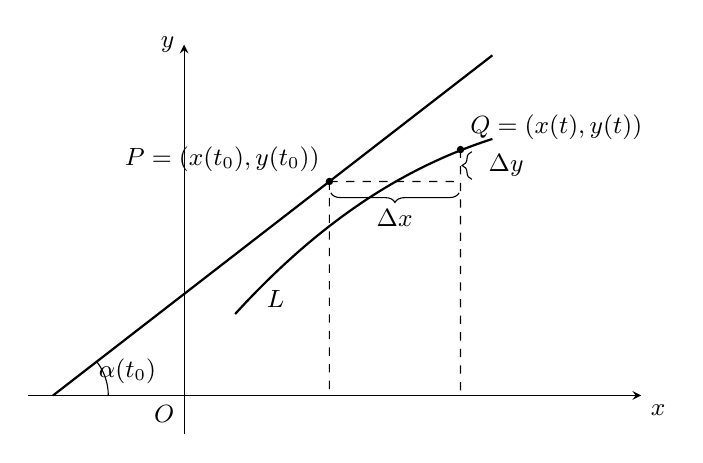
\begin{tikzpicture}[scale=0.9,>=stealth,font=\small]
  \draw[->] (-2.20,0) -- (6.45,0) node[below right] {$x$};
  \draw[->] (0,-0.55) -- (0,4.95) node[left] {$y$};
  \node[below left] at (0,0) {$O$};
  % 曲线 L
  \draw[thick] (0.72,1.15) .. controls (2.00,2.55) and (3.20,3.25) .. (4.35,3.62);
  \node[below left] at (1.55,1.62) {$L$};
  % 切线
  \draw[thick] (-1.85,0) -- (4.35,4.80);
  % P, Q
  \coordinate (P) at (2.05,3.02);
  \coordinate (Q) at (3.90,3.47);
  \fill (P) circle (1.5pt);
  \fill (Q) circle (1.5pt);
  \node[above left] at (P) {$P = (x(t_0), y(t_0))$};
  \node[above right] at (Q) {$Q = (x(t), y(t))$};
  % 虚线
  \draw[dashed] (P) -- (3.90,3.02);
  \draw[dashed] (P) -- (2.05,0);
  \draw[dashed] (Q) -- (3.90,0);
  % Delta x / Delta y
  \draw[decorate,decoration={brace,amplitude=3.5pt,mirror}] (2.07,2.86) -- (3.88,2.86);
  \node at (2.97,2.50) {$\Delta x$};
  \draw[decorate,decoration={brace,amplitude=3.5pt}] (4.06,3.05) -- (4.06,3.44);
  \node[right] at (4.16,3.24) {$\Delta y$};
  % 角 alpha(t0)
  \draw (-1.85,0) ++(0.78,0) arc (0:37.7:0.78);
  \node at (-0.80,0.34) {$\alpha(t_0)$};
\end{tikzpicture}
\caption{}\label{fig:3.2.1}
\end{figure}

如果 $x = x(t)$ 具有反函数 $t = t(x)$, 则
\[
y = y(t) = y(t(x)).
\]
这时只要 $x(t)$, $y(t)$ 可导, $x'(t) \neq 0$ (因而当 $\Delta x \to 0$ 时, 也有 $\Delta t \to 0$ 与 $\Delta y \to 0$), 就有
\[
\frac{\mathrm{d}y}{\mathrm{d}x} = \frac{\mathrm{d}y}{\mathrm{d}t}\cdot\frac{\mathrm{d}t}{\mathrm{d}x} = \frac{\mathrm{d}y}{\mathrm{d}t}\bigg/\frac{\mathrm{d}x}{\mathrm{d}t} = \frac{y'(t)}{x'(t)},\ \text{或}\ y'_{x} = \frac{y'_{t}}{x'_{t}}.
\]
如果 $x(t)$, $y(t)$ 均 2 阶可导, 则
\[
\begin{aligned}
\frac{\mathrm{d}^{2}y}{\mathrm{d}x^{2}} &= \frac{\mathrm{d}}{\mathrm{d}x}\left(\frac{\mathrm{d}y}{\mathrm{d}x}\right) = \frac{\left(\frac{y'(t)}{x'(t)}\right)'}{x'(t)} = \frac{y''(t)x'(t) - y'(t)x''(t)}{x'(t)[x'(t)]^{2}}\\
&= \frac{x'(t)y''(t) - y'(t)x''(t)}{[x'(t)]^{3}}.
\end{aligned}
\]
当曲线 $L$ 由极坐标方程 $\rho = \rho(\theta)$ 表示, 则可用极角 $\theta$ 作为参数, 即
\[
(x, y) = (\rho(\theta)\cos\theta, \rho(\theta)\sin\theta).
\]
如果 $\rho$ 可导, 则曲线 $\rho = \rho(\theta)$ 上点 $M(\rho, \theta)$ 处切线 $MT$ 与极轴 $Ox$ 轴的夹角 $\alpha$ 的正切(即切线斜率)为
\[
\begin{aligned}
\tan\alpha &= \frac{\mathrm{d}y}{\mathrm{d}x} = \frac{y'(\theta)}{x'(\theta)} = \frac{(\rho(\theta)\sin\theta)'}{(\rho(\theta)\cos\theta)'}\\
&= \frac{\rho'(\theta)\sin\theta + \rho(\theta)\cos\theta}{\rho'(\theta)\cos\theta - \rho(\theta)\sin\theta} = \frac{\rho'(\theta)\tan\theta + \rho(\theta)}{\rho'(\theta) - \rho(\theta)\tan\theta}.
\end{aligned}
\]
如图~\ref{fig:3.2.2} 所示, 过点 $M$ 的射线 $OH$ ($O$ 为极点, $Ox$ 为极轴) 与切线 $MT$ 的夹角 $\varphi$ 的正切为
\[
\begin{aligned}
\tan\varphi &= \tan(\alpha - \theta) = \frac{\tan\alpha - \tan\theta}{1 + \tan\alpha\tan\theta}\\
&= \frac{\frac{\rho'(\theta)\tan\theta + \rho(\theta)}{\rho'(\theta) - \rho(\theta)\tan\theta} - \tan\theta}{1 + \frac{\rho'(\theta)\tan\theta + \rho(\theta)}{\rho'(\theta) - \rho(\theta)\tan\theta}\tan\theta}\\
&= \frac{\rho'(\theta)\tan\theta + \rho(\theta) - \rho'(\theta)\tan\theta + \rho(\theta)\tan^{2}\theta}{\rho'(\theta) - \rho(\theta)\tan\theta + \rho'(\theta)\tan^{2}\theta + \rho(\theta)\tan\theta}\\
&= \frac{\rho(\theta)(1 + \tan^{2}\theta)}{\rho'(\theta)(1 + \tan^{2}\theta)} = \frac{\rho(\theta)}{\rho'(\theta)}.
\end{aligned}
\]

\begin{figure}[htbp]
\centering
\begin{tikzpicture}[scale=0.95,>=stealth,font=\small]
  \draw[->] (-1.05,0) -- (5.45,0) node[below right] {$x$};
  \node[below left] at (0,0) {$O$};
  % 射线 OH
  \draw[thick] (0,0) -- (5.00,3.29);
  \node[right] at (5.05,3.35) {$H$};
  % 角 theta
  \draw (0,0) ++(0.95,0) arc (0:33.3:0.95);
  \node at (0.98,0.30) {$\theta$};
  % 曲线
  \draw[thick] (1.86,1.02) .. controls (2.20,1.28) and (2.46,1.53) .. (2.507,1.647)
        .. controls (2.55,1.75) and (2.70,2.55) .. (2.86,3.30);
  % 切线 MT
  \draw[thick] (1.835,0) -- (3.86,4.96);
  \node[right] at (3.82,4.90) {$T$};
  % 点 M
  \fill (2.507,1.647) circle (1.6pt);
  \node[left] at (2.36,1.70) {$M$};
  % 角 alpha
  \draw (1.835,0) ++(0.65,0) arc (0:67.8:0.65);
  \node at (2.30,0.42) {$\alpha$};
  % 角 varphi
  \draw (2.507,1.647) ++(33.3:0.70) arc (33.3:67.8:0.70);
  \node at (3.11,2.38) {$\varphi$};
\end{tikzpicture}
\caption{}\label{fig:3.2.2}
\end{figure}

\begin{example}\label{ex:3.2.9}
证明: 对数螺线 $\rho = \mathrm{e}^{\frac{\theta}{2}}$ 上所有点的切线与向径的夹角 $\varphi$ 为常量.
\end{example}

\begin{proof}
因为
\[
\tan\varphi = \frac{\rho(\theta)}{\rho'(\theta)} = \frac{\mathrm{e}^{\frac{\theta}{2}}}{\frac{1}{2}\mathrm{e}^{\frac{\theta}{2}}} = 2,
\]
所以 $\varphi = \arctan 2$ 为常量.
\end{proof}

\begin{example}\label{ex:3.2.10}
求由上半椭圆的参数方程 $(x, y) = (a\cos t, b\sin t)$, $0 < t < \pi$ 所确定的函数 $y = y(x) = b\sqrt{1 - \frac{x^{2}}{a^{2}}}$ 的导数 $\frac{\mathrm{d}y}{\mathrm{d}x}$ 与 2 阶导数 $\frac{\mathrm{d}^{2}y}{\mathrm{d}x^{2}}$.
\end{example}

\begin{solution}
\[
\frac{\mathrm{d}y}{\mathrm{d}x} = \frac{\mathrm{d}y}{\mathrm{d}t}\bigg/\frac{\mathrm{d}x}{\mathrm{d}t} = \frac{b\cos t}{-a\sin t} = -\frac{b}{a}\cot t.
\]
\[
\frac{\mathrm{d}^{2}y}{\mathrm{d}x^{2}} = \frac{\mathrm{d}}{\mathrm{d}x}\left(\frac{\mathrm{d}y}{\mathrm{d}x}\right) = \frac{-\frac{b}{a}(\cot t)'}{-a\sin t} = \frac{-\frac{b}{a}(-\csc^{2}t)}{-a\sin t} = -\frac{b}{a^{2}\sin^{3}t}.
\]
或直接代入公式得到
\[
\begin{aligned}
\frac{\mathrm{d}^{2}y}{\mathrm{d}x^{2}} &= \frac{x'(t)y''(t) - y'(t)x''(t)}{[x'(t)]^{3}}\\
&= \frac{(-a\sin t)(-b\sin t) - (b\cos t)(-a\cos t)}{(-a\sin t)^{3}}\\
&= -\frac{b}{a^{2}\sin^{3}t}.
\end{aligned}
\]
请读者对 $y = b\sqrt{1 - \frac{x^{2}}{a^{2}}}$ 关于 $x$ 求 1 阶、2 阶导数来验证上述结果.
\end{solution}

\begin{example}\label{ex:3.2.11}
求由摆线参数方程 $(x, y) = (a(t - \sin t), a(1 - \cos t))$ 所确定的函数 $y = y(x)$ 的 2 阶导数.
\end{example}

\begin{solution}
\[
\frac{\mathrm{d}y}{\mathrm{d}x} = \frac{y'(t)}{x'(t)} = \frac{a\sin t}{a(1 - \cos t)} = \frac{2\sin\frac{t}{2}\cos\frac{t}{2}}{2\sin^{2}\frac{t}{2}} = \cot\frac{t}{2},
\]
\[
\frac{\mathrm{d}^{2}y}{\mathrm{d}x^{2}} = \frac{\mathrm{d}}{\mathrm{d}x}\left(\frac{\mathrm{d}y}{\mathrm{d}x}\right) = \frac{\left(\cot\frac{t}{2}\right)'}{a(1 - \cos t)} = \frac{-\frac{1}{2}\csc^{2}\frac{t}{2}}{2a\sin^{2}\frac{t}{2}} = -\frac{1}{4a}\csc^{4}\frac{t}{2}.
\]
\end{solution}

\begin{example}\label{ex:3.2.12}
设曲线参数方程为 $(x, y) = (1 - t^{2}, t - t^{2})$, 求它在 $t = 1$ 处的切线方程与法线方程.
\end{example}

\begin{solution}
因为
\[
\frac{\mathrm{d}y}{\mathrm{d}x}\bigg|_{t=1} = \frac{y'_{t}}{x'_{t}}\bigg|_{t=1} = \frac{1 - 2t}{-2t}\bigg|_{t=1} = \frac{1}{2},
\]
故切线方程为 $y - 0 = \frac{1}{2}(x - 0)$, 即 $y = \frac{1}{2}x$; 法线方程为 $y - 0 = -2(x - 0)$, 即 $y = -2x$.
\end{solution}

\begin{remark}\label{rem:3.2.2}
加速度是位移 $x(t)$ 对时间 $t$ 的 2 阶导数, 这是高阶导数在物理中的应用. 在古典微分几何中, 考虑 2 阶连续可导的正则曲线 $(x(t), y(t))$, 所谓正则指的是 $(x'(t))^{2} + (y'(t))^{2} \neq 0$, 从反映它弯曲程度的曲率公式
\[
\kappa(t) = \frac{x'(t)y''(t) - x''(t)y'(t)}{\left[(x'(t))^{2} + (y'(t))^{2}\right]^{3/2}},
\]
可看出 2 阶导数在几何中的重要应用. 在 3.6 节, 我们还可用 2 阶导数来刻画曲线的凹凸性与拐点以及判断函数的驻点(即 1 阶导数为 0 的点)是否为极值点, 是极大值点还是极小值点.
\end{remark}

\begin{exblock}{练习题 3.2}
  \item 求 $y$ 关于 $x$ 的 2 阶导数 $y''$.
  \begin{enumerate}[label=(\arabic*)]
    \item $y = \mathrm{e}^{-x^{2}}$;
    \item $y = x^{2}a^{x}$ ($a > 0$);
    \item $y = \ln\sin x$;
    \item $y = (1 + x^{2})\arctan x$;
    \item $y = \frac{\arcsin x}{\sqrt{1 - x^{2}}}$;
    \item $y = x\ln x$.
  \end{enumerate}

  \item 
  \begin{enumerate}[label=(\arabic*)]
    \item 设 $f(x) = \mathrm{e}^{2x-1}$, 求 $f''(0)$;
    \item 设 $f(x) = \arctan x$, 求 $f''(1)$;
    \item 设 $f(x) = \sin^{2}x$, 求 $f''\left(\frac{\pi}{2}\right)$;
    \item 设 $f(x) = 3x^{3} + 4x^{2} - 5x - 9$, 求 $f''(1)$, $f'''(1)$, $f^{(4)}(1)$.
  \end{enumerate}

  \item 求下列高阶导数:
  \begin{enumerate}[label=(\arabic*)]
    \item $f(x) = \frac{1+x}{\sqrt{1-x}}$, 求 $f^{(10)}(x)$;
    \item $f(x) = \frac{x^{2}}{1-x}$, 求 $f^{(8)}(x)$;
    \item $f(x) = \mathrm{e}^{-x^{2}}$, 求 $f''(x)$;
    \item $f(x) = \ln(1+x)$, 求 $f^{(5)}(x)$;
    \item $f(x) = x^{3}\mathrm{e}^{x}$, 求 $f^{(10)}(x)$.
  \end{enumerate}

  \item 设函数 $f$ 在 $(-\infty, x_0]$ 上 2 阶可导,
  \[
  F(x) = \begin{cases}f(x), & x \leqslant x_0,\\ a(x-x_0)^{2} + b(x-x_0) + c, & x > x_0.\end{cases}
\]
  问: 当 $a$, $b$, $c$ 为何值时函数 $F$ 在 $\mathbb{R}$ 上有 2 阶导函数.

  \item 设 $f$ 为 2 阶可导函数, 求下列各函数的 2 阶导函数.
  \begin{enumerate}[label=(\arabic*)]
    \item $y = f(\ln x)$;
    \item $y = f(x^{n})$, $n \in \mathbb{N}$;
    \item $y = f(f(x))$.
  \end{enumerate}

  \item 设函数 $f$ 在点 $x = 1$ 处 2 阶可导, $f'(1) = 0$, $f''(1) = 0$. 证明: 在 $x = 1$ 处有
  \[
  \frac{\mathrm{d}}{\mathrm{d}x}f(x^{2}) = \frac{\mathrm{d}^{2}}{\mathrm{d}x^{2}}f^{2}(x).
\]

  \item 求下列函数的 $n$ 阶导数:
  \begin{enumerate}[label=(\arabic*)]
    \item $y = \ln x$;
    \item $y = \frac{\ln x}{x}$;
    \item $y = \frac{1}{x(1-x)}$;
    \item $f(x) = \frac{x^{n}}{1-x}$;
    \item $v = \mathrm{e}^{ax}\sin bx$ ($a$, $b$ 均为实数).
  \end{enumerate}

  \item 设 $y = \frac{ax+b}{cx+d}$. 证明:
  \[
  y^{(n)}(x) = (-1)^{n+1}\frac{n!\,c^{n-1}}{(cx+d)^{n+1}}\begin{vmatrix}a & b\\ c & d\end{vmatrix}.
\]

  \item 证明: 函数
  \[
  f(x) = \begin{cases}\mathrm{e}^{-\frac{1}{x^{2}}}, & x \neq 0,\\ 0, & x = 0\end{cases}
\]
  在 $x = 0$ 处 $n$ 阶可导, 且 $f^{(n)}(0) = 0$, 其中 $n \in \mathbb{N}$.

  \item 求由下列参数方程所确定的函数的 2 阶导数 $\frac{\mathrm{d}^{2}y}{\mathrm{d}x^{2}}$:
  \begin{enumerate}[label=(\arabic*)]
    \item $\begin{cases}x = a\cos^{3}t,\\ y = a\sin^{3}t;\end{cases}$
    \item $\begin{cases}x = \mathrm{e}^{t}\cos t,\\ y = \mathrm{e}^{t}\sin t;\end{cases}$
    \item $\begin{cases}x = \cos^{4}t,\\ y = \sin^{4}t;\end{cases}$
    \item $\begin{cases}x = \frac{t}{1+t},\\ y = \frac{1-t}{1+t}.\end{cases}$
  \end{enumerate}

  \item 证明: 原点到曲线
  \[
  \begin{cases}x = a(\cos t + t\sin t),\\ y = a(\sin t - t\cos t)\end{cases}
\]
  上任一点的法线的距离等于 $a$.

  \item 证明: 圆 $r = 2a\sin\theta$ ($a > 0$) 上任一点的切线与向径的夹角等于向径的极角.

  \item 求心形(脏)线 $r = a(1 + \cos\theta)$ 的切线与切点向径之间的夹角.
\end{exblock}

\begin{exblock}{思考题 3.2}
  \item 设 $m$, $n \in \mathbb{N}$. 证明:
  \[
  \sum_{k=0}^{n}(-1)^{k}\mathrm{C}_{n}^{k}k^{m} = \begin{cases}0, & m \leqslant n-1,\\ (-1)^{n}n!, & m = n.\end{cases}
\]

  \item 设 $u$, $v$, $w$ 都为 $t$ 的可导函数. 试给出 $(uvw)^{(n)}$ 的 Leibniz 公式, 这里 $n \in \mathbb{N}$.

  \item 设 $y = x^{n-1}\mathrm{e}^{\frac{1}{x}}$. 证明:
  \[
  y^{(n)} = \frac{(-1)^{n}}{x^{n+1}}\mathrm{e}^{\frac{1}{x}}.
\]

  \item 设 $y = \arctan x$. 证明:
  \[
  y^{(n)} = \frac{P_{n-1}(x)}{(1+x^{2})^{n}},
\]
  其中 $P_{n-1}$ 为最高次项系数是 $(-1)^{n-1}n!$ 的 $n-1$ 次多项式.

  \item 设 $f(x) = x^{n}\ln x$, $n \in \mathbb{N}$, 求极限
  \[
  \lim_{n\to+\infty}\frac{f^{(n)}\left(\frac{1}{n}\right)}{n!}.
\]

  \item 证明: 在 $\mathbb{R}$ 上不存在可导函数 $f$ 满足 $f^{2}(x) = -x^{3} + x^{2} + 1$.

  \item 证明: 在 $\mathbb{R}$ 上不存在可导函数 $f$ 满足 $f^{2}(x) = x^{2} - 3x + 3$.

  \item 求 $\left(\mathrm{e}^{x}\cos x\right)^{(n)}$ 与 $\left(\mathrm{e}^{x}\sin x\right)^{(n)}$.

  \item 设 $y = (1 + \sqrt{x})^{2n+2}$, $n \in \mathbb{N}$, 求 $y^{(n)}(1)$.

  \item 设多项式 $p$ 只有实零点, 证明: $(p'(x))^{2} \geqslant p(x)p''(x)$ 对一切 $x \in \mathbb{R}$ 成立.

  \item 设 $y = \arctan x$.
  \begin{enumerate}[label=(\arabic*)]
    \item 证明它满足方程 $(1+x^{2})y'' + 2xy' = 0$;
    \item 求 $y^{(n)}(0)$.
  \end{enumerate}

  \item 设 $f(x) = \arctan x$. 证明:
  \[
  f^{(n)}(x) = (n-1)!\cos^{n}f(x)\cdot\sin\left(f(x) + \frac{n\pi}{2}\right).
\]
\end{exblock}

% ====================================================================
%  徐森林、薛春华《数学分析》（第一册）
%  \S3.3  微分中值定理
%  源：原书印刷页 185-198（PDF 物理页 191-204）
%  底本：PaddleOCR-VL-1.6 + 高清影印比对校订
%  规范：全西文半角标点；单一落盘出口 _texout.py
% ====================================================================
\section{微分中值定理}\label{sec:3.3}

这一节主要讨论微分学中重要的 Fermat 定理、Rolle 定理、Lagrange 中值定理以及 Cauchy 中值定理, 它们是研究函数的增减性、凹凸性、极值与最值的基础.

\begin{definition}\label{def:3.3.1}
设 $f$ 定义在区间 $I$ 上, $x_0$ 为 $I$ 的内点, 即 $\exists\delta_0>0$, s.t. $B(x_0;\delta_0)=(x_0-\delta,x_0+\delta)\subset I$. 如果 $x_0$ 有一个开邻域 $B(x_0;\delta)=(x_0-\delta,x_0+\delta)\subset I$, s.t. $f(x_0)$ 为 $f(x)$ 在 $(x_0-\delta,x_0+\delta)$ 中的最大(小)值, 即 $f(x)\leqslant f(x_0)$ ($f(x)\geqslant f(x_0)$), 则称 $f(x_0)$ 为 $f$ 的极大(小)值, $x_0$ 称为 $f$ 的极大(小)值点. 极大值与极小值统称为极值. 极大值点与极小值点统称为极值点.
\end{definition}

如果 $x_0$ 为 $I$ 中的内点, 且为 $f$ 的最大(小)值点, 显然, $x_0$ 为 $f$ 的极大(小)值点. 但是, 反之不一定成立. 例如:
\[
f(x)=\begin{cases}x+1,&-2<x\leqslant0,\\ -x+1,&0<x\leqslant1,\\ 2x-2,&1<x\leqslant2,\end{cases}
\]
$x=0$ 为极大值点但非最大值点, $x=1$ 为极小值点但非最小值点.

注意, 最大(小)值若在区间端点达到, 则它就不是极大(小)值.

极值是局部性质, 而最值是整体性质.

\begin{theorem}[Fermat (1601---1665) 定理]\label{thm:3.3.1}
设 $f$ 在点 $x_0$ 处可导, $x_0$ 为 $f$ 的极值点, 则 $f'(x_0)=0$. 但反之不一定成立.
\end{theorem}

若 $f'(x_0)=0$, 则 $x_0$ 称为 $f$ 的驻点或稳定点.

\begin{proof}
不妨设 $x_0$ 为 $f$ 的极大值点, 即 $\exists\delta>0$, s.t. $f(x)\leqslant f(x_0)$, $\forall x\in(x_0-\delta,x_0+\delta)$. 于是(如图~\ref{fig:3.3.1} 所示),
\[
\frac{f(x)-f(x_0)}{x-x_0}\begin{cases}\geqslant0,&x_0-\delta<x<x_0,\\ \leqslant0,&x_0<x<x_0+\delta.\end{cases}
\]
又因为 $f$ 在点 $x_0$ 处可导, 故
\[
\begin{aligned}
0 &\leqslant\lim_{x\to x_0^-}\frac{f(x)-f(x_0)}{x-x_0}=f'_-(x_0)=f'(x_0)=f'_+(x_0)\\
&=\lim_{x\to x_0^+}\frac{f(x)-f(x_0)}{x-x_0}\leqslant0,
\end{aligned}
\]
\[
f'(x_0)=0.
\]
\end{proof}

建议读者用反证法证明 $f'(x_0)=0$.

反之有反例: $f(x)=x^{3}$, $f'(x)=3x^{2}$, $f'(0)=0$, $0$ 为 $f$ 的驻点, 但由 $f$ 严格增与反证法知, $0$ 不是 $f$ 的极值点.

\begin{remark}\label{rem:3.3.1}
定理~\ref{thm:3.3.1} 中, “可导”条件不能删去.

反例: $y=f(x)=|x|$, 显然 $0$ 为 $f$ 的极小值点(也是最小值点), 但由于 $f$ 在点 $0$ 处不可导, 当然谈不上 $f'(0)=0$.
\end{remark}

\begin{figure}[htbp]
\centering
\begin{tikzpicture}[scale=1.0,>=stealth,font=\small]
  \draw[->] (-1.60,0) -- (6.55,0) node[below right] {$x$};
  \draw[->] (0,-0.85) -- (0,5.70) node[left] {$y$};
  \node[below left] at (0,0) {$O$};
  % 水平切线 y = f(x_0)
  \draw[thick] (-1.25,3.30) -- (4.80,3.30);
  \node[left] at (-1.28,3.30) {$f(x_0)$};
  % 曲线 y = f(x)
  \draw[thick] (0.94,1.88) .. controls (1.55,2.42) and (2.35,3.23) .. (3.06,3.23)
               .. controls (3.85,3.23) and (4.72,2.52) .. (5.61,1.84);
  % 三条竖直虚线
  \draw[dashed] (1.33,3.30) -- (1.33,-1.12);
  \draw[dashed] (2.99,3.30) -- (2.99,-1.12);
  \draw[dashed] (4.80,3.30) -- (4.80,-0.52);
  % 横轴标签
  \node[below] at (1.33,-1.16) {$x_0-\delta$};
  \node[below] at (2.99,-1.16) {$x_0$};
  \node[below] at (4.80,-0.56) {$x_0+\delta$};
\end{tikzpicture}
\caption{}\label{fig:3.3.1}
\end{figure}

\begin{theorem}[Rolle (1652---1719) 定理]\label{thm:3.3.2}
设 $f$ 在 $[a,b]$ 上连续, 在 $(a,b)$ 内可导, $f(a)=f(b)$, 则 $\exists\xi\in(a,b)$, s.t. $f'(\xi)=0$ (即 $(\xi,f(\xi))$ 或 $\xi$ 点处的切线平行于 $x$ 轴, 也平行于 $(a,f(a))$ 与 $(b,f(b))$ 的连线).
\end{theorem}

\begin{proof}
因为 $f$ 在 $[a,b]$ 上连续, 由最值定理知, $f$ 必达到最大值与最小值, 即 $\exists\alpha,\beta\in[a,b]$, s.t. $f(\alpha)\leqslant f(x)\leqslant f(\beta)$, $\forall x\in[a,b]$.

如果 $\alpha,\beta\in\{a,b\}$, 则由 $f(a)=f(b)$ 知, $f(x)=f(a)=f(b)$, $\forall x\in[a,b]$, 即 $f$ 为 $[a,b]$ 上的常值函数. 于是, $\forall\xi\in(a,b)$, $f'(\xi)=0$.

如果 $\alpha,\beta$ 中有一个不是端点, 例如 $\alpha\in(a,b)$, 则由 $f$ 在 $\alpha$ 达到最小值, 它必为极小值, 由 Fermat 定理知, $f'(\alpha)=0$. 因此, $\xi=\alpha$ 为定理所求之点.
\end{proof}

\begin{theorem}[Lagrange (1736---1813) 中值定理]\label{thm:3.3.3}
设 $f$ 在 $[a,b]$ 上连续, 在 $(a,b)$ 内可导, 则 $\exists\xi\in(a,b)$, s.t.
\[
f'(\xi)=\frac{f(b)-f(a)}{b-a}
\]
($(\xi,f(\xi))$ 点处的切线平行 $(a,f(a))$ 与 $(b,f(b))$ 的连线) 或
\[
\begin{aligned}
f(b)-f(a)&=f'(\xi)(b-a)\\
&=f'[a+\theta(b-a)](b-a),
\end{aligned}
\]
其中 $0<\theta=\frac{\xi-a}{b-a}<1$.
\end{theorem}

\begin{figure}[htbp]
\centering
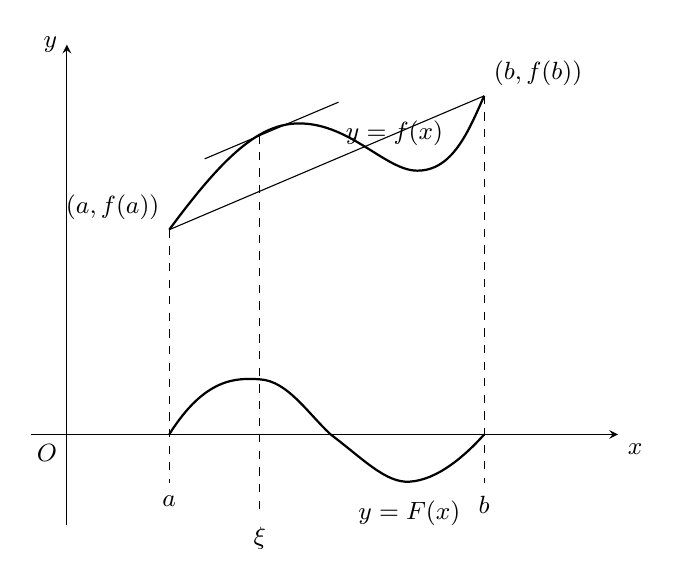
\begin{tikzpicture}[scale=1.0,>=stealth,font=\small]
  \draw[->] (-0.45,0) -- (7.00,0) node[below right] {$x$};
  \draw[->] (0,-1.15) -- (0,4.95) node[left] {$y$};
  \node[below left] at (0,0) {$O$};
  % 曲线 y = f(x)
  \draw[thick] (1.30,2.60) .. controls (2.00,3.55) and (2.45,3.95) .. (2.95,3.95)
               .. controls (3.60,3.95) and (4.05,3.35) .. (4.45,3.35)
               .. controls (4.90,3.35) and (5.10,3.85) .. (5.30,4.30);
  % 弦 (a,f(a)) -- (b,f(b))
  \draw (1.30,2.60) -- (5.30,4.30);
  % 平行于弦的切线 (过 xi 处切点)
  \draw (1.75,3.50) -- (3.45,4.22);
  % 辅助函数 y = F(x)
  \draw[thick] (1.30,0) .. controls (1.75,0.72) and (2.15,0.72) .. (2.45,0.70)
               .. controls (2.80,0.68) and (3.05,0.28) .. (3.35,0.00)
               .. controls (3.75,-0.30) and (4.05,-0.62) .. (4.35,-0.60)
               .. controls (4.70,-0.58) and (5.05,-0.28) .. (5.30,0.00);
  % 三条竖直虚线
  \draw[dashed] (1.30,2.60) -- (1.30,-0.62);
  \draw[dashed] (2.45,3.80) -- (2.45,-1.02);
  \draw[dashed] (5.30,4.30) -- (5.30,-0.62);
  % 标注
  \node[above left] at (1.30,2.60) {$(a,f(a))$};
  \node[above right] at (5.30,4.30) {$(b,f(b))$};
  \node[right] at (3.42,3.82) {$y=f(x)$};
  \node[below] at (4.35,-0.72) {$y=F(x)$};
  \node[below] at (1.30,-0.66) {$a$};
  \node[below] at (2.45,-1.06) {$\xi$};
  \node[below] at (5.30,-0.66) {$b$};
\end{tikzpicture}
\caption{}\label{fig:3.3.2}
\end{figure}

当 $f(a)=f(b)$ 时, $f'(\xi)=\frac{f(b)-f(a)}{b-a}=0$. 因此, Lagrange 中值定理为 Rolle 定理的推广.

\begin{proof}[证法 1]
从图~\ref{fig:3.3.2} 想到令
\[
F(x)=f(x)-\left[f(a)+\frac{f(b)-f(a)}{b-a}(x-a)\right],
\]
则由 $f$ 在 $[a,b]$ 上连续, 在 $(a,b)$ 上可导知, $F$ 在 $[a,b]$ 上连续, 在 $(a,b)$ 上可导, 且
\[
\begin{aligned}
F(a)&=f(a)-\left[f(a)+\frac{f(b)-f(a)}{b-a}(a-a)\right]=0\\
&=f(b)-\left[f(a)+\frac{f(b)-f(a)}{b-a}(b-a)\right]=F(b).
\end{aligned}
\]
根据 Rolle 定理可得, $\exists\xi\in(a,b)$, s.t.
\[
0=F'(\xi)=f'(\xi)-\frac{f(b)-f(a)}{b-a},
\]
\[
f'(\xi)=\frac{f(b)-f(a)}{b-a}.
\]
\end{proof}

\begin{proof}[证法 2]
令
\[
\begin{aligned}
F(x)&=\begin{vmatrix}1&a&f(a)\\1&b&f(b)\\1&x&f(x)\end{vmatrix}=\begin{vmatrix}1&a&f(a)\\0&b-a&f(b)-f(a)\\0&x-a&f(x)-f(a)\end{vmatrix}\\
&=(b-a)[f(x)-f(a)]-(x-a)[f(b)-f(a)],
\end{aligned}
\]
则由 $f$ 在 $[a,b]$ 上连续, 在 $(a,b)$ 内可导知, $F$ 在 $[a,b]$ 上连续, 在 $(a,b)$ 内可导, 且
\[
F(a)=\begin{vmatrix}1&a&f(a)\\1&b&f(b)\\1&a&f(a)\end{vmatrix}=0=\begin{vmatrix}1&a&f(a)\\1&b&f(b)\\1&b&f(b)\end{vmatrix}=F(b).
\]
根据 Rolle 定理知, $\exists\xi\in(a,b)$, s.t.
\[
\begin{aligned}
0=F'(\xi)&=\begin{vmatrix}1&a&f(a)\\1&b&f(b)\\0&1&f'(x)\end{vmatrix}_{x=\xi}=\begin{vmatrix}1&a&f(a)\\0&b-a&f(b)-f(a)\\0&1&f'(\xi)\end{vmatrix}\\
&=(b-a)f'(\xi)-[f(b)-f(a)],
\end{aligned}
\]
\[
f'(\xi)=\frac{f(b)-f(a)}{b-a}.
\]
\end{proof}

\begin{theorem}[Cauchy (1789---1957) 中值定理]\label{thm:3.3.4}
设 $f$, $g$ 在 $[a,b]$ 上连续, 在 $(a,b)$ 内可导, 且 $g'(x)\neq0$, $\forall x\in(a,b)$, 则 $\exists\xi\in(a,b)$, s.t.
\[
\frac{f(b)-f(a)}{g(b)-g(a)}=\frac{f'(\xi)}{g'(\xi)}.
\]
\end{theorem}

特别地, 当 $g(x)=x$ 时, 它就是 Lagrange 中值定理. 因此, Cauchy 中值定理为 Lagrange 中值定理的推广.

\begin{proof}[证法 1]
先证 $g(b)\neq g(a)$.

用反证法. 假设 $g(b)=g(a)$, 由 Rolle 定理知, $\exists\eta\in(a,b)$, s.t. $g'(\eta)=0$, 这与 $g'(x)\neq0$, $\forall x\in(a,b)$ 矛盾. 或由 Lagrange 中值定理知, $\exists\eta\in(a,b)$, s.t. $g(b)-g(a)=g'(\eta)(b-a)\neq0$, 故 $g(b)\neq g(a)$.

仿照定理~\ref{thm:3.3.3} 证法 1, 令
\[
F(x)=f(x)-\left[f(a)+\frac{f(b)-f(a)}{g(b)-g(a)}(g(x)-g(a))\right],
\]
则由 $f$, $g$ 在 $[a,b]$ 上连续, 在 $(a,b)$ 内可导知 $F$ 在 $[a,b]$ 上连续, 在 $(a,b)$ 内可导, 且
\[
\begin{aligned}
F(a)&=f(a)-\left[f(a)+\frac{f(b)-f(a)}{g(b)-g(a)}(g(a)-g(a))\right]=0\\
&=f(b)-\left[f(a)+\frac{f(b)-f(a)}{g(b)-g(a)}(g(b)-g(a))\right]\\
&=F(b).
\end{aligned}
\]
根据 Rolle 定理可得, $\exists\xi\in(a,b)$, s.t.
\[
0=F'(\xi)=f'(\xi)-\frac{f(b)-f(a)}{g(b)-g(a)}g'(\xi),
\]
\[
\frac{f(b)-f(a)}{g(b)-g(a)}=\frac{f'(\xi)}{g'(\xi)}.
\]
\end{proof}

\begin{proof}[证法 2]
仿照定理~\ref{thm:3.3.3} 证法 2, 令
\[
F(x)=\begin{vmatrix}1&g(a)&f(a)\\1&g(b)&f(b)\\1&g(x)&f(x)\end{vmatrix},
\]
则由 $f$, $g$ 在 $[a,b]$ 上连续, 在 $(a,b)$ 内可导知, $F$ 在 $[a,b]$ 上连续, 在 $(a,b)$ 内可导, 且
\[
F(a)=\begin{vmatrix}1&g(a)&f(a)\\1&g(b)&f(b)\\1&g(a)&f(a)\end{vmatrix}=0=\begin{vmatrix}1&g(a)&f(a)\\1&g(b)&f(b)\\1&g(b)&f(b)\end{vmatrix}=F(b).
\]
根据 Rolle 定理可得, $\exists\xi\in(a,b)$, s.t.
\[
\begin{aligned}
0=F'(\xi)&=\begin{vmatrix}1&g(a)&f(a)\\1&g(b)&f(b)\\0&g'(x)&f'(x)\end{vmatrix}_{x=\xi}=\begin{vmatrix}1&g(a)&f(a)\\0&g(b)-g(a)&f(b)-f(a)\\0&g'(\xi)&f'(\xi)\end{vmatrix}\\
&=f'(\xi)[g(b)-g(a)]-g'(\xi)[f(b)-f(a)],
\end{aligned}
\]
\[
\frac{f(b)-f(a)}{g(b)-g(a)}=\frac{f'(\xi)}{g'(\xi)}.
\]
\end{proof}

\begin{corollary}\label{cor:3.3.1}
设 $f$ 在区间 $I$ 上连续, 在 $\mathring{I}$ 内可导, 则
\[
f(x)=c\ (\text{常数})\Longleftrightarrow f'(x)=0,\quad\forall x\in\mathring{I}.
\]
\end{corollary}

\begin{proof}
($\Rightarrow$) 设 $f(x)=c$, $\forall x\in\mathring{I}$, 则 $f'(x)=c'=0$.

($\Leftarrow$) $\forall x_1,x_2\in I$, $x_1<x_2$, 由 $f$ 在 $[x_1,x_2]$ 上连续, 在 $(x_1,x_2)$ 内可导, 以及 Lagrange 中值定理可知, $\exists\xi\in(x_1,x_2)\subset\mathring{I}$, s.t.
\[
\begin{aligned}
f(x_2)-f(x_1)&=f'(\xi)(x_2-x_1)=0\cdot(x_2-x_1)=0,\\
f(x_1)&=f(x_2).
\end{aligned}
\]
因为 $x_1$, $x_2$ 是任取的, 所以, $f(x)=c$ (常数).
\end{proof}

\begin{example}\label{ex:3.3.1}
设
\[
f(x)=\begin{cases}1,&x>0,\\ -1,&x<0.\end{cases}
\]
显然, $f'(x)=0$, 但 $f(x)\neq c$ (常数). 注意: $f$ 的定义域不为一个区间. 因而, 推论~\ref{cor:3.3.1} 充分性的证明中不能应用 Lagrange 中值定理.
\end{example}

\begin{corollary}\label{cor:3.3.2}
设 $f$, $g$ 在区间 $I$ 上的连续, 在 $\mathring{I}$ 内可导, 则
\[
f(x)=g(x)+c\Longleftrightarrow f'(x)=g'(x),\quad\forall x\in\mathring{I},
\]
其中 $c$ 为常数.
\end{corollary}

\begin{proof}
\[
\begin{aligned}
& f(x)=g(x)+c,\ \forall x\in I\\
\Longleftrightarrow\ & f(x)-g(x)=c,\ \forall x\in I\\
\xlongleftrightarrow{\text{推论}~\ref{cor:3.3.1}}\ & f'(x)-g'(x)=[f(x)-g(x)]'=0,\ \forall x\in\mathring{I}\\
\Longleftrightarrow\ & f'(x)=g'(x),\ \forall x\in\mathring{I}.
\end{aligned}
\]
\end{proof}

\begin{corollary}\label{cor:3.3.3}
设 $I_1$, $I_2$ 为两个不相交的非空区间. 则
\[
f(x)=\begin{cases}g(x)+c_1,&x\in I_1,\\ g(x)+c_2,&x\in I_2,\end{cases}\qquad c_1\ \text{与}\ c_2\ \text{为两个无关的常数}
\]
\[
\Longleftrightarrow f'(x)=g'(x),\quad\forall x\in\mathring{I}_1\cup\mathring{I}_2.
\]
\end{corollary}

\begin{proof}
($\Rightarrow$) 显然.

($\Leftarrow$) 因 $f'(x)=g'(x)$, $\forall x\in\mathring{I}_1\cup\mathring{I}_2$, 根据推论~\ref{cor:3.3.1} 知, $\exists c_1,c_2\in\mathbb{R}$, s.t.
\[
f(x)=\begin{cases}g(x)+c_1,&x\in I_1,\\ g(x)+c_2,&x\in I_2.\end{cases}
\]
\end{proof}

\begin{theorem}[Darboux (1842---1917) 导函数介值定理]\label{thm:3.3.5}
设 $f$ 在 $[a,b]$ 内可导, 则对于 $f'_+(a)$ 与 $f'_-(b)$ 之间的一切值 $k$, 必有 $\xi\in[a,b]$, s.t. $f'(\xi)=k$.
\end{theorem}

如果 $f'_+(a)\neq f'_-(b)$, $k\in(\min\{f'_+(a),f'_-(a)\},\max\{f'_+(a),f'_-(a)\})$, 则可取 $\xi\in(a,b)$, s.t. $f'(\xi)=k$.

\begin{proof}[证法 1]
设 $F(x)=f(x)-kx$, 由 $f$ 在 $[a,b]$ 上可导知, $F$ 在 $[a,b]$ 上也可导, 且
\[
F'_+(a)\cdot F'_-(b)=(f'_+(a)-k)(f'_-(b)-k)\leqslant0.
\]
如果 $F'_+(a)\cdot F'_-(b)=0$, 则 $F'_+(a)=0$ 或 $F'_-(b)=0$, 取 $\xi=a$ 或 $b$.

如果 $F'_+(a)\cdot F'_-(b)<0$, 不妨设
\[
\lim_{x\to a^+}\frac{F(x)-F(a)}{x-a}=F'_+(a)>0,
\]
\[
\lim_{x\to b^-}\frac{F(x)-F(b)}{x-b}=F'_-(b)<0,
\]
由保号性定理知, $\exists a_1,b_1$, s.t. $a<a_1<b_1<b$, 且
\[
F(a)<F(a_1),\quad F(b_1)>F(b).\tag*{(*)}
\]
因为 $F$ 在 $[a,b]$ 上可导, 所以它在 $[a,b]$ 上连续. 根据最值定理知, $\exists\xi\in[a,b]$, s.t. $F$ 在 $\xi$ 达到最大值. 由 $(*)$ 式知, $\xi\neq a,b$, 必有 $\xi\in(a,b)$. 因此, $\xi$ 为 $F$ 的极大值点. 再根据 Fermat 定理得到
\[
\begin{aligned}
0=F'(\xi)&=(f(x)-kx)'\big|_{x=\xi}=f'(\xi)-k,\\
f'(\xi)&=k.
\end{aligned}
\]
\end{proof}

\begin{proof}[证法 2]
设
\[
\varphi_1(x)=\begin{cases}\frac{f(x)-f(a)}{x-a},&a<x\leqslant b,\\ f'_+(a),&x=a,\end{cases}
\]
\[
\varphi_2(x)=\begin{cases}\frac{f(x)-f(b)}{x-b},&a\leqslant x<b,\\ f'_-(b),&x=b.\end{cases}
\]
因为
\[
\lim_{x\to a^+}\varphi_1(x)=\lim_{x\to a^+}\frac{f(x)-f(a)}{x-a}=f'_+(a)=\varphi_1(a),
\]
\[
\lim_{x\to b^-}\varphi_2(x)=\lim_{x\to b^-}\frac{f(x)-f(b)}{x-b}=f'_-(b)=\varphi_2(b),
\]
所以, $\varphi_1$, $\varphi_2$ 都在 $[a,b]$ 上连续, 在 $(a,b)$ 内可导.

如果 $k=f'_+(a)$, 取 $\xi=a$; 如果 $k=f'_-(b)$, 取 $\xi=b$. 如果 $f'_+(a)<k<f'_-(b)$ (或 $f'_-(b)<k<f'_+(a)$), 则 $k$ 应介于 $f'_+(a)$ 与 $\frac{f(b)-f(a)}{b-a}$ 之间或介于 $\frac{f(b)-f(a)}{b-a}$ 与 $f'_-(b)$ 之间, 不妨设为前者. 由 $\varphi_1$ 的定义知, $k$ 介于 $\varphi_1(a)$ 与 $\varphi_1(b)$ 之间. 根据 $\varphi_1$ 的连续性及连续函数的介值定理知, $\exists\theta\in[a,b]$, 由 Lagrange 中值定理知, $\exists\xi\in(a,\theta)\subset(a,b)$, s.t.
\[
k=\varphi_1(\theta)=\frac{f(\theta)-f(a)}{\theta-a}=f'(\xi).
\]
\end{proof}

\begin{remark}\label{rem:3.3.2}
注意, Darboux 定理~\ref{thm:3.3.5} 中, $f'(x)$ 不必连续. 如果 $f'$ 连续, 只需将连续函数的介值定理应用于 $f'(x)$ 即得定理~\ref{thm:3.3.5} 的结论.
\end{remark}

\begin{example}\label{ex:3.3.2}
证明: $\forall h>-1$, $h\neq0$ 成立不等式
\[
\frac{h}{1+h}<\ln(1+h)<h.
\]
\end{example}

\begin{proof}
令 $f(x)=\ln(1+x)$, 则由 Lagrange 中值定理, 有
\[
\ln(1+h)=\ln(1+h)-\ln1=\frac{h}{1+\theta h},\quad0<\theta<1.
\]
如果 $h>0$, 由 $0<\theta<1$ 推得
\[
1<1+\theta h<1+h,
\]
\[
\frac{h}{1+h}<\frac{h}{1+\theta h}<h,
\]
\[
\frac{h}{1+h}<\ln(1+h)<h.
\]
如果 $-1<h<0$, 由 $0<\theta<1$ 推得
\[
0<1+h<1+\theta h<1,
\]
\[
\frac{h}{1+h}<\frac{h}{1+\theta h}<h,
\]
\[
\frac{h}{1+h}<\ln(1+h)<h.
\]
\end{proof}

\begin{example}\label{ex:3.3.3}
设 $0<\alpha\leqslant\beta<\frac{\pi}{2}$, 证明:
\[
\frac{\beta-\alpha}{\cos^{2}\alpha}\leqslant\tan\beta-\tan\alpha\leqslant\frac{\beta-\alpha}{\cos^{2}\beta}.
\]
\end{example}

\begin{proof}
当 $\alpha=\beta$ 时, 上述不等式为等式.

当 $\alpha\neq\beta$ 时, 令 $f(x)=\tan x$, $0<\alpha\leqslant x\leqslant\beta<\frac{\pi}{2}$. 由于 $f(x)=\tan x$ 在 $[\alpha,\beta]$ 上连续, 在 $(\alpha,\beta)$ 内可导, 根据 Lagrange 中值定理知, $\exists\xi\in(\alpha,\beta)$, s.t. $\tan\beta-\tan\alpha=(\tan x)'\big|_{x=\xi}(\beta-\alpha)=\sec^{2}\xi\cdot(\beta-\alpha)=\frac{\beta-\alpha}{\cos^{2}\xi}$. 于是,
\[
\begin{aligned}
&\frac{\beta-\alpha}{\cos^{2}\alpha}<\frac{\beta-\alpha}{\cos^{2}\xi}<\frac{\beta-\alpha}{\cos^{2}\beta}.\\
&\frac{\beta-\alpha}{\cos^{2}\alpha}<\tan\beta-\tan\alpha<\frac{\beta-\alpha}{\cos^{2}\beta}.
\end{aligned}
\]
\end{proof}

\begin{example}\label{ex:3.3.4}
证明: $\arctan\frac{1+x}{1-x}=\arctan x+\frac{\pi}{4}$, $|x|<1$.
\end{example}

\begin{proof}
设 $f(x)=\arctan\frac{1+x}{1-x}-\arctan x$, $|x|<1$, 则
\[
\begin{aligned}
f'(x)&=\frac{1}{1+\left(\frac{1+x}{1-x}\right)^{2}}\cdot\frac{(1-x)+(1+x)}{(1-x)^{2}}-\frac{1}{1+x^{2}}\\
&=\frac{2}{(1-x)^{2}+(1+x)^{2}}-\frac{1}{1+x^{2}}=0,\quad|x|<1.
\end{aligned}
\]
根据推论~\ref{cor:3.3.1} 可知,
\[
\arctan\frac{1+x}{1-x}-\arctan x=f(x)=f(0)=\frac{\pi}{4}-0=\frac{\pi}{4},
\]
即
\[
\arctan\frac{1+x}{1-x}=\arctan x+\frac{\pi}{4},\quad|x|<1.
\]
\end{proof}

\begin{example}\label{ex:3.3.5}
设 $f$ 在 $[a,b]$ ($a>0$) 上连续, 在 $(a,b)$ 内可导, 则 $\exists\xi\in(a,b)$, s.t.
\[
f(b)-f(a)=\xi f'(\xi)\ln\frac{b}{a}.
\]
\end{example}

\begin{proof}
令 $g(x)=\ln x$, 显然它在 $[a,b]$ 上连续, 在 $(a,b)$ 内可导,
\[
g'(x)=(\ln x)'=\frac{1}{x}\neq0,\quad\forall x\in(a,b).
\]
由 Cauchy 中值定理, $\exists\xi\in(a,b)$, s.t.
\[
\frac{f(b)-f(a)}{\ln b-\ln a}=\frac{f'(\xi)}{\frac{1}{\xi}},
\]
即
\[
f(b)-f(a)=\xi f'(\xi)\ln\frac{b}{a}.
\]
\end{proof}

\begin{example}\label{ex:3.3.6}
设 $f:\mathbb{R}\to\mathbb{R}$ 可导. 证明: $f(x)=0$ 的任何两相异根之间必有 $f'(x)-af(x)=0$ 的一个根, 其中 $a\in\mathbb{R}$.
\end{example}

\begin{proof}
设 $x_1$, $x_2$ 为 $f(x)=0$ 的两个相异的根, 不妨设 $x_1<x_2$. 令
\[
F(x)=f(x)\mathrm{e}^{-ax},
\]
$F$ 在 $\mathbb{R}$ 上可导, 且
\[
F'(x)=\mathrm{e}^{-ax}[f'(x)-af(x)].
\]
显然,
\[
F(x_1)=f(x_1)\mathrm{e}^{-ax_1}=0=f(x_2)\mathrm{e}^{-ax_2}=F(x_2).
\]
根据 Rolle 定理知, $\exists\xi\in(x_1,x_2)$, s.t.
\[
0=F'(\xi)=\mathrm{e}^{-a\xi}[f'(\xi)-af(\xi)],
\]
即
\[
f'(\xi)-af(\xi)=0,
\]
$\xi$ 为 $f'(x)-af(x)=0$ 的一个根.
\end{proof}

\begin{example}\label{ex:3.3.7}
设 $f$ 在 $[0,a]$ 上 2 阶可导 ($a>0$), $|f''(x)|\leqslant M$, $\forall x\in[0,a]$, 且 $f$ 在 $(0,a)$ 内达到最大值. 证明: $|f'(0)|+|f'(a)|\leqslant Ma$.
\end{example}

\begin{proof}
设 $x_0\in(0,a)$, s.t. $f(x_0)=\max\limits_{0\leqslant x\leqslant a}f(x)$, 则由 Fermat 定理知, $f'(x_0)=0$. 将 Lagrange 中值定理应用于 $f'(x)$, 得: $\exists\xi_1\in(0,x_0)$, $\exists\xi_2\in(x_0,a)$, s.t.
\[
\begin{aligned}
f'(0)&=f'(x_0)+f''(\xi_1)(0-x_0)=-f''(\xi_1)x_0,\\
f'(a)&=f'(x_0)+f''(\xi_2)(a-x_0)=-f''(\xi_2)(a-x_0).
\end{aligned}
\]
因此
\[
\begin{aligned}
|f'(0)|+|f'(a)|&=|f''(\xi_1)x_0|+|f''(\xi_2)(a-x_0)|\\
&\leqslant Mx_0+M(a-x_0)=Ma.
\end{aligned}
\]
\end{proof}

\begin{example}\label{ex:3.3.8}
设 $f:\mathbb{R}\to\mathbb{R}$ 2 阶可导, $|f(x)|\leqslant1$, 且
\[
[f(0)]^{2}+[f'(0)]^{2}=4.
\]
证明: $\exists\xi\in(-2,2)$, s.t. $f(\xi)+f''(\xi)=0$.
\end{example}

\begin{proof}
令 $F(x)=[f(x)]^{2}+[f'(x)]^{2}$, 则
\[
F'(x)=2f'(x)[f(x)+f''(x)].
\]
由 Lagrange 中值定理知, $\exists a\in(-2,0)$, $b\in(0,2)$, s.t.
\[
f'(a)=\frac{f(0)-f(-2)}{0-(-2)}=\frac{f(0)-f(-2)}{2},
\]
\[
f'(b)=\frac{f(2)-f(0)}{2-0}=\frac{f(2)-f(0)}{2}.
\]
于是, 有
\[
\begin{aligned}
|f'(a)|&=\left|\frac{f(0)-f(-2)}{2}\right|\leqslant\frac{1}{2}(|f(0)|+|f(-2)|)\\
&\leqslant\frac{1}{2}(1+1)=1,
\end{aligned}
\]
\[
|F(a)|=[f(a)]^{2}+[f'(a)]^{2}\leqslant1+1=2.
\]
同理有
\[
|f'(b)|\leqslant1,\quad|F(b)|\leqslant2.
\]
因为 $f$ 2 阶可导, 故 $F$ 可导, 当然也连续. 根据最值定理知, $\exists\xi\in[a,b]$, s.t. $F(\xi)=\max\limits_{x\in[a,b]}F(x)$.

由于
\[
\begin{aligned}
&F(a)\leqslant2<4=[f(0)]^{2}+[f'(0)]^{2}=F(0)\leqslant F(\xi),\\
&F(b)\leqslant2<4=F(0)\leqslant F(\xi),
\end{aligned}
\]
故 $\xi\neq a,b$. 由此知 $\xi$ 为 $F$ 的极大值点, 根据 Fermat 定理知,
\[
0=F'(\xi)=2f'(\xi)[f(\xi)+f''(\xi)].
\]
但是,
\[
\begin{aligned}
&1+[f'(\xi)]^{2}\geqslant[f(\xi)]^{2}+[f'(\xi)]^{2}=F(\xi)\geqslant F(0)=4,\\
&[f'(\xi)]^{2}\geqslant4-1=3,\quad f'(\xi)\neq0.
\end{aligned}
\]
因此,
\[
f(\xi)+f''(\xi)=0.
\]
\end{proof}

\begin{example}\label{ex:3.3.9}
设函数 $f$ 在 $[0,1]$ 上连续, 在 $(0,1)$ 内可导, $f(0)=0$, $f(1)=1$. 又设 $k_1$, $\cdots$, $k_n$ 为任意的 $n$ 个正数. 证明: 在 $(0,1)$ 中存在 $n$ 个互不相同的数 $t_1$, $\cdots$, $t_n$, s.t.
\[
\sum_{i=1}^{n}\frac{k_i}{f'(t_i)}=\sum_{i=1}^{n}k_i.
\]
\end{example}

\begin{proof}
令 $y_0=0$, 以及
\[
y_i=\frac{k_1+\cdots+k_i}{k_1+\cdots+k_n},\quad i=1,\cdots,n,
\]
则 $0=y_0<y_1<y_2<\cdots<y_n=1$. 取 $x_0=0$, $x_n=1$. 在 $[0,1]$ 上对连续函数 $f$ 应用介值定理可求得一点 $x_1\in(0,1)$, s.t. $f(x_1)=y_1$. 再在 $[x_1,1]$ 上应用介值定理求得一点 $x_2\in(x_1,1)$, s.t. $f(x_2)=y_2$, 依次有 $f(x_i)=y_i$, $i=0,1,2,\cdots,n$. 在每个小区间 $[x_{i-1},x_i]$ 上, 应用 Lagrange 中值定理, 求得 $t_i\in(x_{i-1},x_i)$ 满足
\[
y_i-y_{i-1}=f(x_i)-f(x_{i-1})=f'(t_i)(x_i-x_{i-1}),
\]
由此得出
\[
\frac{y_i-y_{i-1}}{f'(t_i)}=x_i-x_{i-1},
\]
\[
\begin{aligned}
\sum_{i=1}^{n}\frac{k_i}{f'(t_i)}&=\sum_{i=1}^{n}\frac{y_i-y_{i-1}}{f'(t_i)}(k_1+\cdots+k_n)\\
&=\sum_{i=1}^{n}(x_i-x_{i-1})(k_1+\cdots+k_n)\\
&=(x_n-x_0)\sum_{i=1}^{n}k_i=\sum_{i=1}^{n}k_i.
\end{aligned}
\]
\end{proof}

\begin{example}[导数极限定理]\label{ex:3.3.10}
设 $f$ 在 $(x_0,b)$ 内可导, 且在 $x_0$ 右连续, 又 $f'(x_0^+)$ 存在, 则 $f'_+(x_0)$ 存在, 且 $f'_+(x_0)=f'(x_0^+)$.
\end{example}

\begin{proof}
因为 $f$ 在 $(x_0,b)$ 内可导, 且在 $x_0$ 右连续, 故在 $[x_0,x]\subset[x_0,b)$ 上应用 Lagrange 中值定理知, $\exists\xi(x)\in(x_0,x)$, s.t. $\lim\limits_{x\to x_0^+}\xi(x)=x_0^+$ 且
\[
\begin{aligned}
f'_+(x_0)&=\lim_{x\to x_0^+}\frac{f(x)-f(x_0)}{x-x_0}=\lim_{x\to x_0^+}f'(\xi(x))\\
&=\lim_{u\to x_0^+}f'(u)=f'(x_0^+).
\end{aligned}
\]
\end{proof}

\begin{example}\label{ex:3.3.11}
设 $D(x)$ 为 Dirichlet 函数. 是否有函数 $F(x)$, s.t. $F'(x)=D(x)$, 即 $D(x)$ 是否有原函数.
\end{example}

\begin{solution}
否. (反证) 假设存在函数 $F$, s.t. $F'(x)=D(x)$, 则 $F'(0)=D(0)=1$, $F'(\sqrt{2})=D(\sqrt{2})=0$. 根据 Darboux 定理, $\exists\xi\in(0,1)$, s.t. $\frac{1}{2}=F'(\xi)=D(\xi)=0$ 或 $1$, 矛盾.
\end{solution}

\begin{example}\label{ex:3.3.12}
设 $f$ 在区间 $[a,b]$ 上可导, 则导函数 $f'$ 无第一类间断点.
\end{example}

\begin{proof}[证法 1]
(反证) 假设 $x_0$ 为 $f'(x)$ 的第一类间断点, 则 $f'(x_0^-)$ 与 $f'(x_0^+)$ 存在有限. 因为 $f$ 在点 $x_0$ 处可导, 故 $f$ 在点 $x_0$ 处连续. 根据导数极限定理(例~\ref{ex:3.3.10}), 有
\[
f'(x_0^+)=f'_+(x_0)=f'(x_0)=f'_-(x_0)=f'(x_0^-).
\]
所以, $f'$ 在点 $x_0$ 处连续, 这与 $x_0$ 为 $f'(x)$ 的间断点相矛盾.
\end{proof}

\begin{proof}[证法 2]
(反证) 假设 $x_0$ 为 $f'(x)$ 的第一类间断点, 则 $f'(x_0^-)$ 与 $f'(x_0^+)$ 存在有限, 且 $f'(x_0^-)\neq f'(x_0)$ (或 $f'(x_0^+)\neq f'(x_0)$). 不失一般性, 设 $f'(x_0^-)<f'(x_0)$. 对 $\varepsilon_0=f'(x_0)-f'(x_0^-)>0$, $\exists\delta>0$, 当 $x_0-\delta<x<x_0$ 时,
\[
|f'(x)-f'(x_0^-)|<\frac{\varepsilon_0}{2}=\frac{1}{2}[f'(x_0)-f'(x_0^-)],
\]
\[
f'(x)<f'(x_0^-)+\frac{1}{2}[f'(x_0)-f'(x_0^-)]=\frac{1}{2}[f'(x_0)+f'(x_0^-)].
\]
任取 $x_1\in(x_0-\delta,x_0)$, 则 $f'(x_1)<\frac{1}{2}[f'(x_0)+f'(x_0^-)]$. 在 $[x_1,x_0]$ 中无 $\xi$, s.t. $f'(\xi)=\frac{1}{2}[f'(x_0)+f'(x_0^-)]$, 这与 Darboux 定理(导函数介值定理)的结果相矛盾.
\end{proof}

\begin{remark}\label{rem:3.3.3}
例~\ref{ex:3.3.12} 表明有第一类间断点的函数必无原函数. 但无第一类间断点的不连续函数也未必有原函数, 例~\ref{ex:3.3.11} 中的 Dirichlet 函数解释了这个道理.
\end{remark}

\begin{exblock}{练习题 3.3}
  \item $\forall c\in\mathbb{R}$, 方程 $x^{3}-3x+c=0$ 在 $[0,1]$ 上无相异的根.

  \item 设函数 $f$ 在 $(a,b)$ 上可导, 且 $f(a^+)=f(b^-)$ 有限或 $+\infty$, 或 $-\infty$. 证明: $\exists\xi\in(a,b)$, s.t. $f'(\xi)=0$.

  \item 应用 Lagrange 中值定理证明下列不等式:
  \begin{enumerate}[label=(\arabic*)]
    \item $|\sin x-\sin y|\leqslant|x-y|$, $x,y\in\mathbb{R}$;
    \item $py^{p-1}(x-y)\leqslant x^{p}-y^{p}\leqslant px^{p-1}(x-y)$, 其中 $0<y<x$ 且 $p>1$;
    \item $\frac{a-b}{a}<\ln\frac{a}{b}<\frac{a-b}{b}$, 其中 $0<b<a$;
    \item $\frac{h}{1+h^{2}}<\arctan h<h$, 其中 $h>0$;
    \item $0<\frac{1}{\ln(1+x)}-\frac{1}{x}<1$, $x>0$.
  \end{enumerate}

  \item 设 $f$ 在闭区间 $[a,b]$ 上连续, 在开区间 $(a,b)$ 内 2 阶可导, $f(a)=f(b)=0$, 并且 $\exists c\in(a,b)$, s.t. $f(c)>0$. 证明: $\exists\xi\in(a,b)$, s.t. $f''(\xi)<0$.

  \item 设函数 $f$ 在 $(a,b)$ 内可导, 且 $f'$ 单调. 证明: $f'$ 在 $(a,b)$ 内连续.

  \item 设函数 $f$ 在 $\mathbb{R}$ 上有 $n$ 阶导数, 又 $p$ 为一个 $n$ 次多项式, 最高次项系数为 $a_0$. 如果有互不相同的 $x_i$ 使得 $f(x_i)=p(x_i)$, $i=0,1,\cdots,n$. 证明: $\exists\xi\in\mathbb{R}$, s.t. $a_0=\frac{f^{(n)}(\xi)}{n!}$.

  \item 设实数 $a_0,a_1,\cdots,a_n$ 满足
  \[
  \frac{a_0}{n+1}+\frac{a_1}{n}+\cdots+\frac{a_{n-1}}{2}+a_n=0.
\]
  证明: 多项式函数 $a_0x^{n}+a_1x^{n-1}+\cdots+a_{n-1}x+a_n$ 在 $(0,1)$ 内有一个实零点.

  \item 设函数 $f$ 在开区间 $(0,a)$ 内可导, 且 $f(0^+)=+\infty$. 证明: $f'$ 在 $x=0$ 的右旁无下界.

  \item 设函数 $f$ 在 $[0,1]$ 上有 3 阶导函数, 并且 $f(0)=f(1)=0$. 又设 $F(x)=x^{2}f(x)$. 证明: $\exists\xi\in(0,1)$, s.t. $F''(\xi)=0$.

  \item 设 $f$ 既非常值函数又非线性函数, 且在 $[a,b]$ 上连续可导. 证明: $\exists\xi\in(a,b)$, s.t.
  \[
  |f'(\xi)|>\left|\frac{f(b)-f(a)}{b-a}\right|.
\]

  \item 如果 $\mathbb{R}$ 上的 2 阶可导的函数 $f$ 是微分方程 $y''+y=0$ 的一个解. 证明: $f^{2}+(f')^{2}$ 为一常值函数.

  \item 利用题~11 的结果证明: 微分方程 $y''+y=0$ 的解都具有形式
  \[
  y(x)=\lambda\cos x+\mu\sin x,
\]
  这里 $\lambda$ 与 $\mu$ 为常数.

  \item 已知 $f(1)=1$, 分别就下面的 $f(x)$ 求 $f(2)$.
  \begin{enumerate}[label=(\arabic*)]
    \item $xf'(x)+f(x)=0$, $\forall x\in\mathbb{R}$;
    \item $xf'(x)-f(x)=0$, $\forall x\in\mathbb{R}$.
  \end{enumerate}

  \item 设 $y=f(x)$ 在区间 $(a,b)$ 上可导, $f'(x)\neq0$, $\forall x\in(a,b)$. 证明: $f'(x)$ 在 $(a,b)$ 上恒大于 $0$ 或恒小于 $0$.

  \item 设函数 $f$ 在 $[a,b]$ 上可导. 证明: $\exists\xi\in(a,b)$, s.t.
  \[
  2\xi[f(b)-f(a)]=(b^{2}-a^{2})f'(\xi).
\]

  \item 设 $0<\alpha<\beta<\frac{\pi}{2}$. 证明: $\exists\theta\in(\alpha,\beta)$, s.t.
  \[
  \frac{\sin\alpha-\sin\beta}{\cos\alpha-\cos\beta}=-\cot\theta.
\]

  \item 证明: 若 $x>0$, 则
  \begin{enumerate}[label=(\arabic*)]
    \item $\sqrt{x+1}-\sqrt{x}=\frac{1}{2\sqrt{x+\theta(x)}}$, 其中 $\frac{1}{4}\leqslant\theta(x)\leqslant\frac{1}{2}$;
    \item $\lim\limits_{x\to0}\theta(x)=\frac{1}{4}$, $\lim\limits_{x\to+\infty}\theta(x)=\frac{1}{2}$.
  \end{enumerate}

  \item 设 $f(x)$ 在开区间 $(a,b)$ 内可导, 且 $\lim\limits_{x\to a^+}f(x)=\lim\limits_{x\to b^-}f(x)$ (实数, $+\infty$ 或 $-\infty$). 证明: $\exists\xi\in(a,b)$, s.t. $f'(\xi)=0$.

  \item 设 $f$ 在区间 $I$ 上可导, 且 $|f'(x)|\leqslant M$, $\forall x\in I$, 其中 $M$ 为常数. 证明: $f$ 在 $I$ 上满足 Lipschitz 条件, 即
  \[
  |f(x')-f(x'')|\leqslant M|x'-x''|,\quad\forall x',x''\in I.
\]
  进而推得 $f$ 在 $I$ 上一致连续.

  应用上述结果判断 $f(x)=\begin{cases}x\cos\frac{1}{x},&x>0,\\ 0,&x=0\end{cases}$ 在 $[0,+\infty)$ 上的一致连续性.
\end{exblock}

\begin{exblock}{思考题 3.3}
  \item 设函数 $f$ 在 $[a,b]$ 上连续, 在 $(a,b)$ 上可导, $ab>0$. 试用下列三种方法证明: $\exists\xi\in(a,b)$, s.t.
  \[
  \frac{1}{a-b}\begin{vmatrix}a&b\\ f(a)&f(b)\end{vmatrix}=f(\xi)-\xi f'(\xi).
\]
  \begin{enumerate}[label=(\arabic*)]
    \item 对 $F(x)=\frac{f(x)}{x}$, $G(x)=\frac{1}{x}$ 应用 Cauchy 中值定理;
    \item 对 $F(x)=xf\left(\frac{ab}{x}\right)$ 应用 Lagrange 中值定理;
    \item 对 $F(x)=\begin{vmatrix}1&\frac{1}{x}&\frac{f(x)}{x}\\ 1&\frac{1}{a}&\frac{f(a)}{a}\\ 1&\frac{1}{b}&\frac{f(b)}{b}\end{vmatrix}$ 应用 Rolle 定理.
  \end{enumerate}

  \item 设 $f(x)=(x-x_0)^{r}g(x)$, $g$ 在点 $x_0$ 处连续, 且 $g(x_0)\neq0$, 则称 $x_0$ 为 $f$ 的 $r$ 重根, 其中 $r=0,1,2,\cdots$.
  \begin{enumerate}[label=(\arabic*)]
    \item 如果 $g$ 可导, $x_0$ 为 $f$ 的 $r$ 重根. 证明: $x_0$ 必为 $f'(x)$ 的 $r-1$ 重根.
    \item 设 $f$ 为 $n$ 阶可导函数, 如果 $f(x)=0$ 有 $n+1$ 个相异的实根. 证明: 方程 $f^{(n)}(x)=0$ 至少有一个实根.
    \item 设 $f$ 为可导函数, 如果 $f(x)=0$ 有 $s$ 个相异的实根 $x_1,\cdots,x_s$, 它们的重数分别为 $r_1,\cdots,r_s$, 且 $r_1+\cdots+r_s=r$ (称 $f(x)=0$ 按重数计恰有 $r$ 个根). 证明: $f'(x)=0$ 按重数计恰有 $r-1$ 个根.
    \item 设 $f$ 为 $n$ 阶可导函数, 如果 $f(x)=0$ 按重数计恰有 $n+1$ 个实根. 证明: 方程 $f^{(n)}(x)=0$ 至少有一个实根.
  \end{enumerate}

  \item 设函数 $f$ 在 $[a,b]$ 上连续, 在 $(a,b)$ 内可导, 且 $f(a)=f(b)=0$. 证明: $\exists\xi\in(a,b)$, s.t.
  \[
  f(\xi)+f'(\xi)=0.
\]

  \item 设 $f$ 与 $g$ 在 $[a,b]$ 上连续, 在 $(a,b)$ 内可导, 且 $f(a)=f(b)=0$. 证明: $\exists\xi\in(a,b)$, s.t.
  \[
  f'(\xi)+f(\xi)g'(\xi)=0.
\]
  提示: (1) 令 $F(x)=f(x)\mathrm{e}^{g(x)}$, 并应用 Rolle 定理; (2) 令 $F(x)=\ln f(x)+g(x)$, 并应用 Fermat 定理.

  \item 设 $f:[0,1]\to\mathbb{R}$ 连续, 在 $(0,1)$ 内可导, $f(0)=0$, 且 $\forall x\in(0,1)$, 都有 $f(x)\neq0$. 证明: $\exists\xi\in(0,1)$, s.t.
  \[
  \frac{nf'(\xi)}{f(\xi)}=\frac{f'(1-\xi)}{f(1-\xi)},
\]
  其中 $n$ 为自然数.

  提示: (1) 令 $F(x)=f^{n}(x)f(1-x)$, 并应用 Rolle 定理; (2) 令 $F(x)=n\ln f(x)+\ln f(1-x)$, $x\in(0,1)$, 并应用 Fermat 定理.

  \item 设函数 $f$ 在 $[a,+\infty)$ 上连续, 在 $(a,+\infty)$ 内可导, $f(a)<0$, 且当 $x>a$ 时, $f'(x)>k>0$. 证明: $f$ 有唯一的零点.

  \item 设函数 $f(x)$ 在 $[0,1]$ 上连续, 在 $(0,1)$ 内可导, 且 $\forall x\in(0,1)$, 有 $|f'(x)|<1$ 及 $f(0)=f(1)$. 证明: $\forall x_1,x_2\in[0,1]$, 有 $|f(x_2)-f(x_1)|<\frac{1}{2}$.

  \item 设 $f(x)$ 在 $[a,+\infty)$ 上可导, 且 $\lim\limits_{x\to+\infty}\frac{f(x)}{x}=0$. 证明: $\lim\limits_{x\to+\infty}|f'(x)|=0$. 并构造函数 $f(x)$ 满足上述条件, 但 $\varlimsup\limits_{x\to+\infty}|f'(x)|>0$.

  \item 设 $f(x)$ 在 $(a,+\infty)$ 上有有界的导函数. 应用 Lagrange 中值定理证明: $\lim\limits_{x\to+\infty}\frac{f(x)}{x\ln x}=0$.
\end{exblock}

% ====================================================================
%  徐森林、薛春华《数学分析》（第一册）
%  \S3.4  L'Hospital 法则
%  源：原书印刷页 198-206（PDF 物理页 204-212）
%  底本：PaddleOCR-VL-1.6 + 高清影印比对校订
%  规范：全西文半角标点；单一落盘出口 _texout.py
% ====================================================================
\section{L'Hospital 法则}\label{sec:3.4}

本节介绍的 L'Hospital(洛必塔)法则是求 $\frac{0}{0}$, $\frac{\infty}{\infty}$, $0\cdot\infty$, $0^{0}$, $1^{\infty}$, $\infty^{0}$, $\infty-\infty$ 各种不定型极限的非常有效的方法.

\begin{theorem}[$\frac{0}{0}$ 不定型极限, L'Hospital 法则]\label{thm:3.4.1}
设 $f$, $g$ 在区间 $(x_0,b)$ 上可导, 且
\[
\lim_{x\to x_0^{+}}f(x)=0=\lim_{x\to x_0^{+}}g(x),\quad g'(x)\neq0,\quad \forall x\in(x_0,b).
\]
如果 $\lim\limits_{x\to x_0^{+}}\frac{f'(x)}{g'(x)}=A$(实数, $\pm\infty$, $\infty$), 那么
\[
\lim_{x\to x_0^{+}}\frac{f(x)}{g(x)}=\lim_{x\to x_0^{+}}\frac{f'(x)}{g'(x)}=A.
\]
\end{theorem}

\begin{proof}
延拓 $f$, $g$ 到 $x_0$, s.t. $f(x_0)=g(x_0)=0$, 则 $f$, $g$ 在 $[x_0,b]$ 上连续, 且 $\forall x\in(x_0,b)$, $g'(x)\neq0$. 根据 Cauchy 中值定理知, $\exists\xi\in(x_0,x)$, s.t.
\[
\frac{f(x)}{g(x)}=\frac{f(x)-f(x_0)}{g(x)-g(x_0)}=\frac{f'(\xi)}{g'(\xi)}.
\]
令 $x\to x_0^{+}$, 此时, $\xi\to x_0^{+}$, 所以,
\[
\lim_{x\to x_0^{+}}\frac{f(x)}{g(x)}=\lim_{x\to x_0^{+}}\frac{f'(\xi)}{g'(\xi)}=\lim_{x\to x_0^{+}}\frac{f'(x)}{g'(x)}.
\]
\end{proof}

\begin{remark}\label{rem:3.4.1}
当 $x\to x_0^{-}$, $x\to x_0$ 时, 类似定理~\ref{thm:3.4.1}, 有相同的结论.
\end{remark}

\begin{theoremp}[$\frac{0}{0}$ 不定型极限, L'Hospital 法则]\label{thm:3.4.1p}
设 $f$, $g$ 在 $(a,+\infty)$ 上可导, 且
\[
\lim_{x\to+\infty}f(x)=0=\lim_{x\to+\infty}g(x),\quad g'(x)\neq0,\quad \forall x\in(a,+\infty).
\]
如果 $\lim\limits_{x\to+\infty}\frac{f'(x)}{g'(x)}=A$(实数, $\pm\infty$, $\infty$), 那么
\[
\lim_{x\to+\infty}\frac{f(x)}{g(x)}=\lim_{x\to+\infty}\frac{f'(x)}{g'(x)}=A.
\]
\end{theoremp}

\begin{proof}
令 $x=\frac{1}{t}$, 当 $x\to+\infty$ 时, $t\to0^{+}$, 则
\[
\lim_{x\to+\infty}f(x)=0\Longleftrightarrow\lim_{t\to0^{+}}f\left(\frac{1}{t}\right)=0,
\]
\[
\lim_{x\to+\infty}g(x)=0\Longleftrightarrow\lim_{t\to0^{+}}f\left(\frac{1}{t}\right)=0.
\]
于是,
\[
\begin{aligned}
\lim_{x\to+\infty}\frac{f(x)}{g(x)}&=\lim_{t\to0^{+}}\frac{f\left(\frac{1}{t}\right)}{g\left(\frac{1}{t}\right)}=\lim_{t\to0^{+}}\frac{f'\left(\frac{1}{t}\right)\cdot\frac{-1}{t^{2}}}{g'\left(\frac{1}{t}\right)\cdot\frac{-1}{t^{2}}}=\lim_{t\to0^{+}}\frac{f'\left(\frac{1}{t}\right)}{g'\left(\frac{1}{t}\right)}\\
&=\lim_{x\to+\infty}\frac{f'(x)}{g'(x)}.
\end{aligned}
\]
\end{proof}

\begin{remarkp}\label{rem:3.4.1p}
当 $x\to-\infty$, $x\to\infty$ 时, 类似定理~\ref{thm:3.4.1p} 有相同的结论.
\end{remarkp}

\begin{theorempp}[$\frac{0}{0}$ 不定型极限, 推广 L'Hospital 法则]\label{thm:3.4.1pp}
设当 $x\to x_0^{+}$ 时, $\frac{f}{g}$, $\frac{f'}{g'}$, $\cdots$, $\frac{f^{(n-1)}}{g^{(n-1)}}$ 均为 $\frac{0}{0}$ 型, 且 $g^{(i)}(x)\neq0$, $i=1,\cdots,n$. 如果 $\lim\limits_{x\to x_0^{+}}\frac{f^{(n)}(x)}{g^{(n)}(x)}=A$(实数, $\pm\infty$, $\infty$), 则
\[
\lim_{x\to x_0^{+}}\frac{f(x)}{g(x)}=\lim_{x\to x_0^{+}}\frac{f'(x)}{g'(x)}=\cdots=\lim_{x\to x_0^{+}}\frac{f^{(n)}(x)}{g^{(n)}(x)}=A.
\]
\end{theorempp}

\begin{proof}
由题设将定理~\ref{thm:3.4.1} 应用于 $f^{(n-1)}(x)$, $g^{(n-1)}(x)$ 推出
\[
\lim_{x\to x_0^{+}}\frac{f^{(n-1)}(x)}{g^{(n-1)}(x)}=\lim_{x\to x_0^{+}}\frac{f^{(n)}(x)}{g^{(n)}(x)}.
\]
依此类推得到
\[
\lim_{x\to x_0^{+}}\frac{f(x)}{g(x)}=\lim_{x\to x_0^{+}}\frac{f'(x)}{g'(x)}=\cdots=\lim_{x\to x_0^{+}}\frac{f^{(n-1)}(x)}{g^{(n-1)}(x)}=\lim_{x\to x_0^{+}}\frac{f^{(n)}(x)}{g^{(n)}(x)}.
\]
\end{proof}

\begin{remarkpp}\label{rem:3.4.1pp}
当 $x\to x_0^{-}$, $x\to x_0$, $x\to\pm\infty$, $x\to\infty$ 时, 类似定理~\ref{thm:3.4.1pp} 有相同的结论.
\end{remarkpp}

\begin{theorem}[$\frac{\cdot}{\infty}$ 不定型极限, L'Hospital 法则]\label{thm:3.4.2}
设 $f$, $g$ 都在 $(x_0,b)$ 上可导, 且
\[
\lim_{x\to x_0^{+}}g(x)=\infty,\quad g'(x)\neq0,\quad \forall x\in(x_0,b).
\]
如果 $\lim\limits_{x\to x_0^{+}}\frac{f'(x)}{g'(x)}=A$(实数, $\pm\infty$, $\infty$), 那么
\[
\lim_{x\to x_0^{+}}\frac{f(x)}{g(x)}=\lim_{x\to x_0^{+}}\frac{f'(x)}{g'(x)}=A.
\]
\end{theorem}

\begin{proof}[证法 1]
只证 $\lim\limits_{x\to x_0^{+}}\frac{f'(x)}{g'(x)}=A\in\mathbb{R}$ 的情形, 其他情形 $(A=\pm\infty,\infty)$ 类似证明.

$\forall\varepsilon>0$, $\exists b_1\in(x_0,b)$, s.t. 当 $x\in(x_0,b_1)$ 时,
\[
A-\frac{\varepsilon}{2}<\frac{f'(x)}{g'(x)}<A+\frac{\varepsilon}{2}.
\]
因此, 根据 Cauchy 中值定理, $\exists\xi\in(x,b_1)$, s.t.
\[
\begin{aligned}
A-\frac{\varepsilon}{2}<\left(\frac{f(x)}{g(x)}-\frac{f(b_1)}{g(x)}\right)\left(1-\frac{g(b_1)}{g(x)}\right)^{-1}&=\frac{f(x)-f(b_1)}{g(x)-g(b_1)}\\
&=\frac{f'(\xi)}{g'(\xi)}<A+\frac{\varepsilon}{2},\\
\left(1-\frac{g(b_1)}{g(x)}\right)\left(A-\frac{\varepsilon}{2}\right)+\frac{f(b_1)}{g(x)}&<\frac{f(x)}{g(x)}\\
&<\left(1-\frac{g(b_1)}{g(x)}\right)\left(A+\frac{\varepsilon}{2}\right)+\frac{f(b_1)}{g(x)}.
\end{aligned}
\]
又因为 $\lim\limits_{x\to x_0}g(x)=\infty$, 故
\[
\lim_{x\to x_0^{+}}\left[\left(1-\frac{g(b_1)}{g(x)}\right)\left(A-\frac{\varepsilon}{2}\right)+\frac{f(b_1)}{g(x)}\right]=A-\frac{\varepsilon}{2},
\]
\[
\lim_{x\to x_0^{+}}\left[\left(1-\frac{g(b_1)}{g(x)}\right)\left(A+\frac{\varepsilon}{2}\right)+\frac{f(b_1)}{g(x)}\right]=A+\frac{\varepsilon}{2}.
\]
由此知, $\exists b_2\in(x_0,b_1)$, s.t. 当 $x\in(x_0,b_2)$ 时,
\[
A-\varepsilon<\frac{f(x)}{g(x)}<A+\varepsilon.
\]
这就证明了
\[
\lim_{x\to x_0^{+}}\frac{f(x)}{g(x)}=A=\lim_{x\to x_0^{+}}\frac{f'(x)}{g'(x)}.
\]
\end{proof}

\begin{proof}[证法 2]
在不等式
\[
\begin{aligned}
&\left(1-\frac{g(b_1)}{g(x)}\right)\left(A-\frac{\varepsilon}{2}\right)+\frac{f(b_1)}{g(x)}<\frac{f(x)}{g(x)}\\
&<\left(1-\frac{g(b_1)}{g(x)}\right)\left(A+\frac{\varepsilon}{2}\right)+\frac{f(b_1)}{g(x)}
\end{aligned}
\]
两边取上、下极限得到
\[
A-\frac{\varepsilon}{2}\leqslant\varliminf_{x\to x_0^{+}}\frac{f(x)}{g(x)}\leqslant\varlimsup_{x\to x_0^{+}}\frac{f(x)}{g(x)}\leqslant A+\frac{\varepsilon}{2},
\]
再令 $\varepsilon\to0^{+}$, 有
\[
A\leqslant\varliminf_{x\to x_0^{+}}\frac{f(x)}{g(x)}\leqslant\varlimsup_{x\to x_0^{+}}\frac{f(x)}{g(x)}\leqslant A,
\]
\[
\lim_{x\to x_0}\frac{f(x)}{g(x)}=\lim_{x\to x_0^{+}}\frac{f(x)}{g(x)}=\varlimsup_{x\to x_0^{+}}\frac{f(x)}{g(x)}=A=\lim_{x\to x_0}\frac{f'(x)}{g'(x)}.
\]
\end{proof}

注意: 定理~\ref{thm:3.4.2} 中, 当 $x\to x_0^{+}$ 时, $\frac{\cdot}{\infty}$ 的分子可以趋于 $\infty$, 也可以不趋于 $\infty$.

关于 $\frac{\cdot}{\infty}$ 不定型极限, 类似定理~\ref{thm:3.4.1p}、定理~\ref{thm:3.4.1pp}、注~\ref{rem:3.4.1}、注~\ref{rem:3.4.1p}、注~\ref{rem:3.4.1pp} 可得到定理 3.4.2$'$、定理 3.4.2$''$、注 3.4.2$'$、注 3.4.2$''$, 不再一一赘述.

\begin{example}\label{ex:3.4.1}
在例~\ref{ex:2.2.13} 中, 应用 L'Hospital 法则得到
\[
\lim_{x\to+\infty}\frac{\ln x}{x^{k}}=\lim_{x\to+\infty}\frac{1}{x}\cdot\frac{1}{kx^{k-1}}=\frac{1}{k}\lim_{x\to+\infty}\frac{1}{x^{k}}=0,\quad k>0.
\]
\[
\begin{aligned}
\lim_{x\to+\infty}\frac{x^{k}}{a^{x}}&=\lim_{x\to+\infty}\frac{kx^{k-1}}{a^{x}\ln a}=\lim_{x\to+\infty}\frac{k(k-1)x^{k-2}}{a^{x}(\ln a)^{2}}=\cdots\\
&=k(k-1)\cdots(k-n+1)\lim_{x\to+\infty}\frac{x^{k-n}}{a^{x}(\ln a)^{n}}=0,
\end{aligned}
\]
其中, $n-1<k\leqslant n$, $a>1$.

进而, 当 $p(x)=a_0x^{n}+\cdots+a_{n-1}x+a_{n}$ 为多项式时,
\[
\begin{aligned}
\lim_{x\to+\infty}\frac{p(x)}{a^{x}}&=\lim_{x\to+\infty}\frac{p'(x)}{a^{x}\ln a}=\lim_{x\to+\infty}\frac{p''(x)}{a^{x}(\ln a)^{2}}=\cdots\\
&=\lim_{x\to+\infty}\frac{a_0n!}{a^{x}(\ln a)^{n}}=0,\quad a>0.
\end{aligned}
\]
此外, 还有
\[
\lim_{x\to+\infty}\frac{a^{x}}{x^{x}}=\lim_{x\to+\infty}\mathrm{e}^{x(\ln a-\ln x)}=0,\quad a>0.
\]
得到这一等式时, 根本不需要用 L'Hospital 法则. 实际上, 用 L'Hospital 法则不能求得极限.
\end{example}

\begin{example}\label{ex:3.4.2}
\[
\lim_{x\to0}\frac{x-\sin x}{\frac{x^{3}}{3!}}=\lim_{x\to0}\frac{1-\cos x}{\frac{x^{2}}{2!}}=\lim_{x\to0}\frac{\sin x}{x}=1.
\]
必须提醒读者注意: 加减不能用等价代换, 请检查下述计算哪一步是错误的.
\[
\lim_{x\to0}\frac{x-\sin x}{\frac{x^{3}}{3!}}=\lim_{x\to0}\frac{x-x}{\frac{x^{3}}{3!}}=\lim_{x\to0}0=0.
\]
\end{example}

在计算极限时, 会遇到“$0\cdot\infty$”、“$\infty-\infty$”、“$0^{0}$”、“$\infty^{0}$”、“$1^{\infty}$”等不定型. 只要经过适当的变换, 最终都可以化为“$\frac{0}{0}$”或“$\frac{\infty}{\infty}$”型的情形, 再应用 L'Hospital 法则去解决.

\begin{example}\label{ex:3.4.3}
求极限 $\lim\limits_{x\to0^{+}}x^{\alpha}\ln x$, 其中 $\alpha>0$.
\end{example}

\begin{solution}
\[
\begin{aligned}
\lim_{x\to0^{+}}x^{\alpha}\ln x&\xlongequal{0\cdot\infty}\lim_{x\to0^{+}}\frac{\ln x}{\left(\frac{1}{x}\right)^{\alpha}}\xlongequal{\frac{\infty}{\infty}}\lim_{x\to0^{+}}\frac{\frac{1}{x}}{\alpha x^{-\alpha-1}}\\
&=-\frac{1}{\alpha}\lim_{x\to0^{+}}x^{\alpha}=0.
\end{aligned}
\]
\end{solution}

\begin{example}\label{ex:3.4.4}
求极限:
(1) $\lim\limits_{x\to1}\left(\frac{1}{x-1}-\frac{1}{\ln x}\right)$; \quad (2) $\lim\limits_{x\to\pi/2}(\sec x-\tan x)$.
\end{example}

\begin{solution}
这都是“$\infty-\infty$”型, 但可化为 $\frac{0}{0}$ 型.

(1)
\[
\begin{aligned}
\lim_{x\to1}\left(\frac{1}{x-1}-\frac{1}{\ln x}\right)&=\lim_{x\to1}\frac{\ln x-(x-1)}{(x-1)\ln x}=\lim_{x\to1}\frac{\frac{1}{x}-1}{\frac{x-1}{x}+\ln x}\\
&=\lim_{x\to1}\frac{1-x}{x-1+x\ln x}=\lim_{x\to1}\frac{-1}{1+1+\ln x}=-\frac{1}{2}.
\end{aligned}
\]

(2)
\[
\lim_{x\to\pi/2}(\sec x-\tan x)=\lim_{x\to\pi/2}\frac{1-\sin x}{\cos x}=\lim_{x\to\pi/2}\frac{-\cos x}{-\sin x}=0.
\]
\end{solution}

\begin{example}\label{ex:3.4.5}
求极限:
(1) $\lim\limits_{x\to0^{+}}(\sin x)^{x}$; \quad (2) $\lim\limits_{x\to0^{+}}(\sin x)^{\frac{k}{1+\ln x}}$ ($k$ 为常数);
(3) $\lim\limits_{x\to0}(\cos x)^{\frac{1}{x^{2}}}$; \quad (4) $\lim\limits_{x\to\frac{\pi}{2}^{-}}(\tan x)^{\frac{\pi}{2}-x}$.
\end{example}

\begin{solution}
(1)
\[
\begin{aligned}
\lim_{x\to0^{+}}(\sin x)^{x}&\xlongequal{0^{0}}\exp\left(\lim_{x\to0^{+}}x\ln\sin x\right)\xlongequal{0\cdot\infty}\exp\left(\lim_{x\to0^{+}}\frac{\ln\sin x}{x^{-1}}\right)\\
&=\exp\left(\lim_{x\to0^{+}}\frac{1}{-x^{-2}}\cdot\frac{\cos x}{\sin x}\right)=\exp\left(\lim_{x\to0^{+}}\frac{-x}{\sin x}\cdot x\cos x\right)=\mathrm{e}^{0}=1.
\end{aligned}
\]

(2)
\[
\begin{aligned}
\lim_{x\to0^{+}}(\sin x)^{\frac{k}{1+\ln x}}&\xlongequal{0^{0}}\exp\left(\lim_{x\to0^{+}}\frac{k\ln\sin x}{1+\ln x}\right)=\exp^{k}\left(\lim_{x\to0^{+}}\frac{\frac{\cos x}{\sin x}}{x^{-1}}\right)\\
&=\exp^{k}\left(\lim_{x\to0^{+}}\cos x\cdot\frac{x}{\sin x}\right)=\mathrm{e}^{k}.
\end{aligned}
\]

(3)
\[
\lim_{x\to0}(\cos x)^{\frac{1}{x^{2}}}\xlongequal{1^{\infty}}\exp\left(\lim_{x\to0}\frac{\ln\cos x}{x^{2}}\right)=\exp\left(\lim_{x\to0}\frac{-\tan x}{2x}\right)=\mathrm{e}^{-\frac{1}{2}}.
\]

(4)
\[
\begin{aligned}
\lim_{x\to\frac{\pi}{2}^{-}}(\tan x)^{\frac{\pi}{2}-x}&\xlongequal{t=\frac{\pi}{2}-x}\lim_{t\to0^{+}}\left(\frac{\cos t}{\sin t}\right)^{t}=\frac{\lim\limits_{t\to0^{+}}(\cos t)^{t}}{\lim\limits_{t\to0^{+}}(\sin t)^{t}}\\
&=\frac{1}{1}=1.
\end{aligned}
\]
\end{solution}

应用 L'Hospital 法则, 可重新计算例~\ref{ex:2.2.12}(3) 及例~\ref{ex:2.2.13}(3) 中的极限.

\begin{example}\label{ex:3.4.6}
(1) 求 $\lim\limits_{x\to+\infty}\left(1+\frac{1}{n}-\frac{1}{n^{2}}\right)^{n}$;
(2) 求 $\lim\limits_{x\to0^{+}}\left(\frac{a_1^{x}+\cdots+a_m^{x}}{m}\right)^{\frac{1}{x}}$.
\end{example}

\begin{solution}
(1)
\[
\begin{aligned}
\lim_{x\to+\infty}\left(1+\frac{1}{n}-\frac{1}{n^{2}}\right)^{n}&\xlongequal{1^{\infty}}\lim_{x\to0}(1+x-x^{2})^{\frac{1}{x}}\\
&=\exp\left(\lim_{x\to0}\frac{\ln(1+x-x^{2})}{x}\right)=\exp\left(\lim_{x\to0}\frac{1-2x}{1+x-x^{2}}\right)=\mathrm{e}^{1}=\mathrm{e}.
\end{aligned}
\]

(2)
\[
\begin{aligned}
\lim_{x\to0^{+}}\left(\frac{a_1^{x}+\cdots+a_m^{x}}{m}\right)^{\frac{1}{x}}&\xlongequal{1^{\infty}}\exp\left(\lim_{x\to0^{+}}\frac{\ln(a_1^{x}+\cdots+a_m^{x})-\ln m}{x}\right)\\
&=\exp\left(\lim_{x\to0^{+}}\frac{a_1^{x}\ln a_1+\cdots+a_m^{x}\ln a_m}{a_1^{x}+\cdots+a_m^{x}}\right)\\
&=\exp\left(\frac{\ln a_1+\cdots+\ln a_m}{m}\right)=\mathrm{e}^{\ln\sqrt[m]{a_1\cdots a_m}}=\sqrt[m]{a_1\cdots a_m}.
\end{aligned}
\]
\end{solution}

注意: 不能在数列形式下直接用 L'Hospital 法则, 因为对离散变量 $n\in\mathbb{N}$ 是无法求导数的.

\begin{example}\label{ex:3.4.7}
设
\[
f(x)=\begin{cases}\frac{g(x)}{x}, & x\neq0,\\ 0, & x=0,\end{cases}
\]
且 $g(0)=g'(0)=0$, $g''(0)=3$. 试求 $f'(0)$.
\end{example}

\begin{solution}
\[
\begin{aligned}
f'(0)&=\lim_{x\to0}\frac{f(x)-f(0)}{x-0}=\lim_{x\to0}\frac{\frac{g(x)}{x}-0}{x-0}=\lim_{x\to0}\frac{g(x)}{x^{2}}\\
&\xlongequal{\frac{0}{0}}\lim_{x\to0}\frac{g'(x)}{2x}=\frac{1}{2}\lim_{x\to0}\frac{g'(x)-g'(0)}{x-0}=\frac{1}{2}g''(0)=\frac{3}{2}.
\end{aligned}
\]
如果用两次 L'Hospital 法则, 得到
\[
f'(0)=\lim_{x\to0}\frac{g(x)}{x^{2}}=\lim_{x\to0}\frac{g'(x)}{2x}=\lim_{x\to0}\frac{g''(x)}{2}=\frac{1}{2}g''(0)=\frac{3}{2}.
\]
错在何处?
\end{solution}

\begin{example}\label{ex:3.4.8}
设 $f$ 在点 $x$ 处 2 阶可导. 证明:
\[
f''(x)=\lim_{h\to0}\frac{f(x+h)-f(x-h)-2f(x)}{h^{2}}.
\]
\end{example}

\begin{proof}
因为 $f$ 在 $x$ 点 2 阶可导, 故 $\exists\delta>0$, s.t. $f$ 在 $(x-\delta,x+\delta)$ 中 1 阶可导. 于是,
\[
\begin{aligned}
&\lim_{h\to0}\frac{f(x+h)+f(x-h)-2f(x)}{h^{2}}\xlongequal[\text{L'Hospital 法则}]{\frac{0}{0}}\lim_{h\to0}\frac{f'(x+h)-f'(x-h)}{2h}\\
&=\frac{1}{2}\lim_{h\to0}\left[\frac{f'(x+h)-f'(x)}{h}+\frac{f'(x-h)-f'(x)}{-h}\right]=\frac{1}{2}(f''(x)+f''(x))=f''(x).
\end{aligned}
\]
\end{proof}

\begin{example}\label{ex:3.4.9}
下面两种计算哪个是正确的? 如果有错误, 请指出错在何处?
\[
\lim_{x\to+\infty}\frac{2x-\cos x}{2x+\cos x}=\lim_{x\to+\infty}\frac{2-\frac{\cos x}{x}}{2+\frac{\cos x}{x}}=\frac{2-0}{2+0}=1.
\]
\[
\begin{aligned}
\lim_{x\to+\infty}\frac{2x-\cos x}{2x+\cos x}&\xlongequal{\frac{\infty}{\infty}\text{ 型}}\lim_{x\to+\infty}\frac{2+\sin x}{2-\sin x}=\lim_{x\to+\infty}\frac{\cos x}{-\cos x}\\
&=\lim_{x\to+\infty}(-1)=-1.
\end{aligned}
\]
\end{example}

\begin{example}\label{ex:3.4.10}
设 $f$ 在 $(a,+\infty)$ 上可导, 并且 $\lim\limits_{x\to+\infty}[f(x)+f'(x)]=0$. 证明: $\lim\limits_{x\to+\infty}f(x)=0$.
\end{example}

\begin{proof}[证法 1]
由 $\frac{\cdot}{\infty}$ 型 L'Hospital 法则得
\[
\begin{aligned}
\lim_{x\to+\infty}f(x)&=\lim_{x\to+\infty}\frac{\mathrm{e}^{x}f(x)}{\mathrm{e}^{x}}\xlongequal{\frac{\cdot}{\infty}}\lim_{x\to+\infty}\frac{\mathrm{e}^{x}[f(x)+f'(x)]}{\mathrm{e}^{x}}\\
&=\lim_{x\to+\infty}[f(x)+f'(x)]=0.
\end{aligned}
\]
\end{proof}

\begin{proof}[证法 2]
因为 $\lim\limits_{x\to+\infty}[f(x)+f'(x)]=0$, 所以, $\exists\Delta_1>a$, s.t. 当 $x>\Delta_1$ 时, 有
\[
|f(x)+f'(x)|<\frac{\varepsilon}{2}.
\]
固定 $\Delta_1$, 取 $\Delta>\max\left\{\Delta_1,\ln\frac{2|\mathrm{e}^{\Delta_1}f(\Delta_1)|}{\varepsilon}\right\}$, 当 $x>\Delta$ 时, 有
\[
\begin{aligned}
|f(x)-0|&=\left|\frac{\mathrm{e}^{x}f(x)}{\mathrm{e}^{x}}\right|\\
&=\left|\frac{\mathrm{e}^{x}f(x)-\mathrm{e}^{\Delta_1}f(\Delta_1)}{\mathrm{e}^{x}-\mathrm{e}^{\Delta_1}}\cdot\frac{\mathrm{e}^{x}-\mathrm{e}^{\Delta_1}}{\mathrm{e}^{x}}+\frac{\mathrm{e}^{\Delta_1}f(\Delta_1)}{\mathrm{e}^{x}}\right|
\end{aligned}
\]
\[
\begin{aligned}
&\xlongequal[\exists\xi\in(\Delta_1,x)]{\text{Cauchy 中值定理}}\left|\frac{\mathrm{e}^{\xi}[f(\xi)+f'(\xi)]}{\mathrm{e}^{\xi}}(1-\mathrm{e}^{\Delta_1-x})+\frac{\mathrm{e}^{\Delta_1}f(\Delta_1)}{\mathrm{e}^{x}}\right|\\
&\leqslant|f(\xi)+f'(\xi)|+\frac{|\mathrm{e}^{\Delta_1}f(\Delta_1)|}{\mathrm{e}^{x}}<\frac{\varepsilon}{2}+\frac{|\mathrm{e}^{\Delta_1}f(\Delta_1)|}{\mathrm{e}^{\Delta}}\\
&<\frac{\varepsilon}{2}+\frac{\varepsilon}{2}=\varepsilon,
\end{aligned}
\]
所以,
\[
\lim_{x\to+\infty}f(x)=0.
\]
\end{proof}

\begin{exblock}{练习题 3.4}
  \item 求下列不定型的极限:
  \begin{enumerate}[label=(\arabic*)]
    \item $\lim\limits_{x\to0}\frac{\mathrm{e}^{x}-1}{\sin x}$;
    \item $\lim\limits_{x\to\frac{\pi}{6}}\frac{1-2\sin x}{\cos 3x}$;
    \item $\lim\limits_{x\to0}\frac{\ln(1+x)-x}{\cos x-1}$;
    \item $\lim\limits_{x\to0}\frac{\tan x-x}{x-\sin x}$;
    \item $\lim\limits_{x\to\frac{\pi}{2}}\frac{\tan x-6}{\sec x+5}$;
    \item $\lim\limits_{x\to0}\left(\frac{1}{x}-\frac{1}{\mathrm{e}^{x}-1}\right)$;
    \item $\lim\limits_{x\to0}(\tan x)^{\sin x}$;
    \item $\lim\limits_{x\to1}x^{\frac{1}{1-x}}$;
    \item $\lim\limits_{x\to0}(1+x^{2})^{\frac{1}{x}}$;
    \item $\lim\limits_{x\to0^{+}}\sin x\ln x$;
    \item $\lim\limits_{x\to0}\left(\frac{1}{x^{2}}-\frac{1}{\sin^{2}x}\right)$;
    \item $\lim\limits_{x\to0}\left(\frac{\tan x}{x}\right)^{\frac{1}{x^{2}}}$;
    \item $\lim\limits_{x\to0}\frac{\mathrm{e}^{ax}-\mathrm{e}^{bx}}{\sin ax-\sin bx}$;
    \item $\lim\limits_{x\to0}\frac{x\cot x-1}{x^{2}}$;
    \item $\lim\limits_{x\to0}\frac{x(\mathrm{e}^{x}+1)-2(\mathrm{e}^{x}-1)}{x^{3}}$;
    \item $\lim\limits_{x\to+\infty}\frac{\mathrm{e}^{x}+\mathrm{e}^{-x}}{x^{3}}$;
    \item $\lim\limits_{x\to0^{+}}x^{x}$;
    \item $\lim\limits_{x\to1^{-}}\ln x\ln(1-x)$;
    \item $\lim\limits_{x\to+\infty}\left(\cos\frac{a}{x}\right)^{x}$;
    \item $\lim\limits_{x\to+\infty}\left(\frac{2}{\pi}\arctan x\right)^{x}$;
    \item $\lim\limits_{x\to\infty}x\left(\left(1+\frac{1}{x}\right)^{x}-\mathrm{e}\right)$;
    \item $\lim\limits_{x\to\infty}\left(\frac{2}{\pi}\arccos x\right)^{\frac{1}{x}}$;
    \item $\lim\limits_{x\to\infty}(\pi-2\arctan x)\ln x$;
    \item $\lim\limits_{x\to+\infty}\left(\frac{\pi}{2}-\arctan x\right)^{\frac{1}{\ln x}}$;
    \item $\lim\limits_{x\to0}\left(\frac{\ln(1+x)^{1+x}}{x^{2}}-\frac{1}{x}\right)$.
  \end{enumerate}

  \item 设 $f$ 在 $0$ 的某开邻域内 2 阶连续可导且 $f(0)=0$, 定义
  \[
  g(x)=\begin{cases}\frac{f(x)}{x}, & x\neq0,\\ f'(0), & x=0.\end{cases}
\]
  证明: $g$ 在这开邻域内是连续可导的.

  \item (1) 设函数 $f$ 在 $x_0$ 处具有连续的 2 阶导数. 两次应用 L'Hospital 法则证明:
  \[
  \lim_{h\to0}\frac{f(x_0+h)+f(x_0-h)-2f(x_0)}{h^{2}}=f''(x_0);
\]
  (2) 当函数 $f$ 在点 $x_0$ 处具有 2 阶导数时, 上述等式是否仍成立.

  \item 设 $f(0)=0$, $f'$ 在原点的某开邻域内连续, 且 $f'(0)\neq0$. 证明: $\lim\limits_{x\to0^{+}}x^{f(x)}=1$.

  \item 证明: $f(x)=x^{3}\mathrm{e}^{-x^{2}}$ 为有界函数.
\end{exblock}

\begin{exblock}{思考题 3.4}
  \item 设 $x_1=\sin x_0>0$, $x_{n+1}=\sin x_n$, $x\in\mathbb{N}$. 证明:
  \[
  \lim_{n\to+\infty}\sqrt{\frac{n}{3}}x_n=1.
\]

  \item 应用 L'Hospital 法则或数学归纳法证明:
  \[
  \lim_{x\to0}\frac{1-\cos a_1x\cdots\cos a_nx}{x^{2}}=\frac{1}{2}\sum_{k=1}^{n}a_k^{2}.
\]
\end{exblock}

% ==================================================================
%  徐森林、薛春华《数学分析》（第一册）
%  \S3.5  应用导数研究函数之一: 单调性、极值、最值
% ==================================================================
%  源：原书印刷页 206-221（PDF 物理页 212-227）
%  底本：PaddleOCR-VL-1.6 + 高清影印比对校订
%  规范：全西文半角标点；单一落盘出口 _texout.py
% ==================================================================
\section{应用导数研究函数之一: 单调性、极值、最值}\label{sec:3.5}

作为 Fermat 定理、Rolle 定理、Lagrange 中值定理与 Cauchy 中值定理的应用, 我们来研究函数的单调性、极值、最值以及凹凸性.

\begin{theorem}\label{thm:3.5.1}
设 $I$ 为区间, $f$ 在 $I$ 上连续, 在 $\mathring{I}$ 内可导, 且 $f'(x)>0(<0)$, 则 $f$ 在 $I$ 上严格增(减). 反之不真.
\end{theorem}

\begin{proof}
$\forall x_{1},x_{2}\in I$, $x_{1}<x_{2}$, 由 Lagrange 中值定理, $\exists\xi\in(x_{1},x_{2})\subset I$, s.t.
\[
\frac{f(x_{2})-f(x_{1})}{x_{2}-x_{1}}=f'(\xi)>0,
\]
所以, $f(x_{1})<f(x_{2})$, 即 $f$ 在 $I$ 上严格增.

当 $f'(x)<0$ 时, 类似证明, 或用 $-f$ 代替 $f$ 即可证得.

反之不真, 有反例: $f(x)=x^{3}$ 在 $(-\infty,+\infty)$ 上严格增, 但 $f'(0)=3x^{2}|_{x=0}=0$.
\end{proof}

\begin{theorem}\label{thm:3.5.2}
设 $I$ 为区间, $f$ 在 $I$ 上连续, 在 $\mathring{I}$ 内可导, 则
\[
f\ \text{在}\ I\ \text{上单调增(减)}\Longleftrightarrow f'(x)\geqslant 0(\leqslant 0),\ \forall x\in\mathring{I}.
\]
\end{theorem}

\begin{proof}
($\rightarrow$) $\forall x\in\mathring{I}$, 因 $f$ 在 $I$ 上单调增, 故
\[
\frac{f(x+\Delta x)-f(x)}{\Delta x}\geqslant 0,
\]
所以,
\[
f'(x)=\lim_{\Delta x\to 0}\frac{f(x+\Delta x)-f(x)}{\Delta x}\geqslant 0.
\]

($\leftarrow$) $\forall x_{1},x_{2}\in I$, $x_{1}<x_{2}$, 由 Lagrange 中值定理知, $\exists\xi\in(x_{1},x_{2})\subset\mathring{I}$, s.t.
\[
\frac{f(x_{2})-f(x_{1})}{x_{2}-x_{1}}=f'(\xi)\geqslant 0,
\]
所以, $f(x_{1})\leqslant f(x_{2})$, 即 $f$ 在 $I$ 上单调增.

当 $f'(x)\leqslant 0$ 时, 类似证明, 或用 $-f$ 代替 $f$ 即可证得.
\end{proof}

\begin{theorem}\label{thm:3.5.3}
设 $I$ 为区间, $f$ 在 $I$ 上连续, 在 $\mathring{I}$ 内可导, 则 $f$ 在 $I$ 上严格增(减) $\Longleftrightarrow$
(1) $f'(x)\geqslant 0(\leqslant 0)$, $\forall x\in\mathring{I}$; (2) $\{x\in\mathring{I}\mid f'(x)=0\}$ 不构成区间, 或在任何非退化区间 $I_{1}\subset\mathring{I}$ 上, $f'(x)\neq 0$.
\end{theorem}

\begin{proof}
($\rightarrow$) (1) 因为 $f$ 严格增, 当然是单调增, 由定理~\ref{thm:3.5.2} 知, $f'(x)\geqslant 0$, $\forall x\in\mathring{I}$.

(2) (反证) 假设有非退化区间 $I_{1}\subset\mathring{I}$, s.t. $f'(x)=0$, $\forall x\in I_{1}$, 则由推论~\ref{cor:3.3.1} 知, $f(x)=$ 常数, $\forall x\in I_{1}$, 这与 $f$ 严格增相矛盾.

($\leftarrow$) 由右边的条件(1)与定理~\ref{thm:3.5.2} 推得 $f$ 单调增, 故 $\forall x_{1},x_{2}\in I$, $x_{1}<x_{2}$, 有 $f(x_{1})\leqslant f(x_{2})$.

如果 $f(x_{1})=f(x_{2})$, 由 $f$ 单调增知, $f(x)=f(x_{1})$, $\forall x\in[x_{1},x_{2}]$, 所以 $f'(x)=0$, $\forall x\in(x_{1},x_{2})=I_{1}$, 这与右边条件(2)相矛盾. 因此, $\forall x_{1},x_{2}\in I$, $x_{1}<x_{2}$, 有
\[
f(x_{1})<f(x_{2}),
\]
这就证明了 $f$ 在 $I$ 上是严格增的.

关于严格减的情形可类似证明, 或用 $-f$ 代替 $f$ 即可证得.
\end{proof}

\begin{example}\label{ex:3.5.1}
证明 $f(x)=x^{3}$ 在 $(-\infty,+\infty)$ 上是严格增的.
\end{example}

\begin{proof}[证法 1]
因为 $f'(x)=3x^{2}\geqslant 0$, 且 $\{x\mid f'(x)=3x^{2}=0\}=\{0\}$ 不构成区间, 根据定理~\ref{thm:3.5.3} 知, $f(x)=x^{3}$ 在 $(-\infty,+\infty)$ 是严格增的.
\end{proof}

\begin{proof}[证法 2]
对 $x_{1}<x_{2}$, 有
\[
\begin{aligned}
x_{2}^{3}-x_{1}^{3}&=(x_{2}-x_{1})(x_{2}^{2}+x_{2}x_{1}+x_{1}^{2})\\
&=(x_{2}-x_{1})[(|x_{2}|-|x_{1}|)^{2}+2|x_{2}x_{1}|+x_{2}x_{1}]>0,
\end{aligned}
\]
故 $f(x_{1})=x_{1}^{3}<x_{2}^{3}=f(x_{2})$, 即 $f$ 在 $(-\infty,+\infty)$ 是严格增的.
\end{proof}

\begin{example}\label{ex:3.5.2}
证明 $f(x)=x-\sin x$ 在 $(-\infty,+\infty)$ 上严格增.
\end{example}

\begin{proof}
由于 $f'(x)=1-\cos x\geqslant 0$, 且 $\{x\mid f'(x)=1-\cos x=0\}=\{2k\pi\mid k=0,\pm 1,\pm 2,\cdots\}$ 不构成区间, 根据定理~\ref{thm:3.5.3} 知, $f(x)=x-\sin x$ 在 $(-\infty,+\infty)$ 是严格增的.
\end{proof}

\begin{example}\label{ex:3.5.3}
讨论函数 $f(x)=x^{3}-x=x(x+1)(x-1)$ 的单调区间.
\end{example}

\begin{solution}
由于 $f'(x)=3x^{2}-1=(\sqrt{3}x+1)(\sqrt{3}x-1)$, 故驻点为 $x_{1}=-\frac{1}{\sqrt{3}}$, $x_{2}=\frac{1}{\sqrt{3}}$. 应用定理~\ref{thm:3.5.3} 以及下表知, $f$ 在 $\left(-\infty,-\frac{1}{\sqrt{3}}\right)$ 中严格增; 在 $\left(-\frac{1}{\sqrt{3}},\frac{1}{\sqrt{3}}\right)$ 中严格减; 在 $\left(\frac{1}{\sqrt{3}},+\infty\right)$ 中又严格增.

列成表如下:
\begin{center}
\begin{tabular}{|c|c|c|c|c|c|c|c|}
\hline
$x$ & $-\infty$ & & $-\frac{1}{\sqrt{3}}$ & & $\frac{1}{\sqrt{3}}$ & & $+\infty$ \\
\hline
$\sqrt{3}x+1$ & & $-$ & & $+$ & & $+$ & \\
\hline
$\sqrt{3}x-1$ & & $-$ & & $-$ & & $+$ & \\
\hline
$f'(x)$ & & $+$ & & $-$ & & $+$ & \\
\hline
$f(x)$ & & $\nearrow$ & & $\searrow$ & & $\nearrow$ & \\
\hline
\end{tabular}
\end{center}

\begin{figure}[htbp]
\centering
\begin{minipage}[t]{0.50\textwidth}
\begin{gather*}
f(-1)=f(0)=f(1)=0,\\
f\Big(\frac{1}{\sqrt{3}}\Big)=-\frac{2}{3\sqrt{3}}=-\frac{2\sqrt{3}}{9},\\
f\Big(-\frac{1}{\sqrt{3}}\Big)=-f\Big(\frac{1}{\sqrt{3}}\Big)=\frac{2\sqrt{3}}{9},\\
\lim_{x\to-\infty}f(x)=\lim_{x\to-\infty}x^{3}\Big(1-\frac{1}{x^{2}}\Big)=-\infty,\\
\lim_{x\to+\infty}f(x)=\lim_{x\to+\infty}x^{3}\Big(1-\frac{1}{x^{2}}\Big)=+\infty.
\end{gather*}
\end{minipage}
\hfill
\begin{minipage}[t]{0.47\textwidth}
\centering
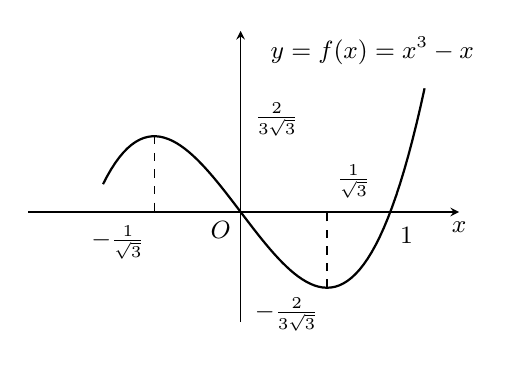
\begin{tikzpicture}[>=stealth,font=\small,x=1.9cm,y=2.5cm,
  baseline=(current bounding box.north)]
  \draw[->] (-1.42,0) -- (1.46,0) node[below] {$x$};
  \draw[->] (0,-0.56) -- (0,0.92);
  \node[below left] at (0,0) {$O$};
  \draw[thick] plot[domain=-0.92:1.23,samples=80] (\x,{(\x)^3-(\x)});
  \draw[dashed] (-0.577,0.385) -- (-0.577,0);
  \draw[dashed] (0.577,-0.385) -- (0.577,0);
  \node[right] at (0.03,0.47) {$\frac{2}{3\sqrt{3}}$};
  \node[right] at (0.03,-0.52) {$-\frac{2}{3\sqrt{3}}$};
  \node[below left] at (-0.577,-0.02) {$-\frac{1}{\sqrt{3}}$};
  \node[above right] at (0.577,0.02) {$\frac{1}{\sqrt{3}}$};
  \node[below right] at (1.0,-0.03) {$1$};
  \node[above] at (0.88,0.70) {$y=f(x)=x^{3}-x$};
\end{tikzpicture}
\caption{}\label{fig:3.5.1}
\end{minipage}
\end{figure}

由上可见, $-\frac{1}{\sqrt{3}}$ 与 $\frac{1}{\sqrt{3}}$ 分别为 $f(x)$ 在 $(-\infty,+\infty)$ 上的极大值点与极小值点 (如图~\ref{fig:3.5.1} 所示).
\end{solution}

\begin{example}\label{ex:3.5.4}
设 $n\in\mathbb{N}$, 证明:
\[
\mathrm{e}^{x}>1+\frac{x}{1!}+\frac{x^{2}}{2!}+\cdots+\frac{x^{n}}{n!},\quad\forall x>0.
\]
\end{example}

\begin{proof}
(数学归纳法) 当 $n=1$ 时, 令 $\varphi(x)=\mathrm{e}^{x}-(1+x)$, $x\geqslant 0$, 则 $\varphi'(x)=\mathrm{e}^{x}-1>0$, $x>0$. 这表明 $\varphi$ 在 $[0,+\infty)$ 上是严格增的. 于是,
\[
\mathrm{e}^{x}-(1+x)=\varphi(x)>\varphi(0)=0,
\]
\[
\mathrm{e}^{x}>1+x,\ x>0.
\]
不等式成立.

假设 $n=k$ 时, 有
\[
\mathrm{e}^{x}>1+\frac{x}{1!}+\frac{x^{2}}{2!}+\cdots+\frac{x^{k}}{k!},\quad x>0,
\]
则当 $n=k+1$ 时, 令
\[
\psi(x)=\mathrm{e}^{x}-\Big[1+\frac{x}{1!}+\frac{x^{2}}{2!}+\cdots+\frac{x^{k+1}}{(k+1)!}\Big],\quad x\geqslant 0.
\]
依归纳假设,
\[
\psi'(x)=\mathrm{e}^{x}-\Big(1+\frac{x}{1!}+\cdots+\frac{x^{k}}{k!}\Big)>0,\quad x>0.
\]
这表明 $\psi$ 在 $[0,+\infty)$ 上是严格增的. 于是,
\[
\psi(x)>\psi(0)=0,
\]
即
\[
\mathrm{e}^{x}>1+\frac{x}{1!}+\frac{x^{2}}{2!}+\cdots+\frac{x^{k}}{k!},\quad x>0.
\]
\end{proof}

\begin{example}\label{ex:3.5.5}
证明: $\frac{2}{\pi}\leqslant\frac{\sin x}{x}<1$, $x\in\left(0,\frac{\pi}{2}\right]$.
\end{example}

\begin{proof}
令 $f(x)=\frac{\sin x}{x}$, 则 $f'(x)=\frac{x\cos x-\sin x}{x^{2}}=\cos x\cdot\frac{x-\tan x}{x}<0$, $x\in\left(0,\frac{\pi}{2}\right)$, 从而 $f(x)$ 在 $\left(0,\frac{\pi}{2}\right]$ 上严格减. 又因为 $\lim\limits_{x\to 0}\frac{\sin x}{x}=1$, 所以
\[
\frac{2}{\pi}=\frac{\sin\frac{\pi}{2}}{\frac{\pi}{2}}\leqslant\frac{\sin x}{x}<1,\quad x\in\left(0,\frac{\pi}{2}\right].
\]
\end{proof}

\begin{example}\label{ex:3.5.6}
设 $f$ 在 $(a,+\infty)$ 上有有界的导函数. 证明: 存在常数 $C$ 与 $x_{0}$, 当 $x\geqslant x_{0}$ 时, $f(x)<Cx$.
\end{example}

\begin{proof}
设 $|f'(x)|\leqslant M$, $\forall x\in(a,+\infty)$. 取定 $x_{0}>0$, 再取 $C>\max\left\{M,\frac{f(x_{0})}{x_{0}}\right\}$. 令 $F(x)=f(x)-Cx$, 则
\[
F'(x)=f'(x)-C<0,
\]
根据定理~\ref{thm:3.5.1} 知, $F(x)$ 在 $(a,+\infty)$ 上严格减. 所以,
\[
f(x)-Cx=F(x)\leqslant F(x_{0})=f(x_{0})-Cx_{0}<0,\ \forall x\geqslant x_{0},
\]
即
\[
f(x)<Cx,\ \forall x\geqslant x_{0}.
\]
\end{proof}

\begin{example}\label{ex:3.5.7}
设 $f$ 在 $[a,+\infty)$ 上连续, 在 $(a,+\infty)$ 内可导, $f(a)<0$, 且当 $x>a$ 时, $f'(x)>k>0$. 证明: $f$ 有惟一的零点.
\end{example}

\begin{proof}
由 $f(a)<0$ 与 $k>0$ 知, $a-\frac{f(a)}{k}>a$. 在 $\left[a,a-\frac{f(a)}{k}\right]$ 上应用 Lagrange 中值定理, $\exists\xi\in\left(a,a-\frac{f(a)}{k}\right)$, s.t.
\[
\begin{aligned}
f\Big(a-\frac{f(a)}{k}\Big)-f(a)&=f'(\xi)\Big[\Big(a-\frac{f(a)}{k}\Big)-a\Big]\\
&=f'(\xi)\cdot\frac{-f(a)}{k}>k\cdot\frac{-f(a)}{k}\\
&=-f(a).
\end{aligned}
\]
因此得到 $f\left(a-\frac{f(a)}{k}\right)>0$. 根据零值定理可知, $\exists c\in\left(a,a-\frac{f(a)}{k}\right)$, s.t. $f(c)=0$.

另一方面, 由题设知, 当 $x>a$ 时, $f'(x)>k>0$, 因此, $f$ 在 $[a,+\infty)$ 上严格增, 从而 $f(x)=0$ 至多只有一个零点.

综上所述可推得 $f$ 有惟一的零点.
\end{proof}

\begin{example}\label{ex:3.5.8}
当 $x>0$ 时, 证明:
\[
\begin{aligned}
x-\frac{x^{3}}{3!}+\frac{x^{5}}{5!}-\cdots-\frac{x^{4k+3}}{(4k+3)!}&<\sin x\\
<x-\frac{x^{3}}{3!}+\frac{x^{5}}{5!}-\cdots-\frac{x^{4k-1}}{(4k-1)!}&+\frac{x^{4k+1}}{(4k+1)!},\\
1-\frac{x^{2}}{2!}+\frac{x^{4}}{4!}-\cdots-\frac{x^{4k+2}}{(4k+2)!}&<\cos x\\
<1-\frac{x^{2}}{2!}+\frac{x^{4}}{4!}-\cdots-\frac{x^{4k+2}}{(4k+2)!}&+\frac{x^{4k+4}}{(4k+4)!}.
\end{aligned}
\]
\end{example}

\begin{proof}
(1) 令 $F_{0}(x)=x-\sin x$, 则 $F'_{0}(x)=1-\cos x\geqslant 0$, 又 $\{x\in(0,+\infty)\mid F'(x)=1-\cos x=0\}=\{2k\pi\mid k\in\mathbb{N}\}$ 不构成区间, 根据定理~\ref{thm:3.5.3} 知, $F_{0}$ 在 $[0,+\infty)$ 上严格增. 于是,
\[
x-\sin x=F_{0}(x)>F(0)=0,
\]
即
\[
\sin x<x,\quad\forall x>0.
\]

(2) 令 $G_{0}(x)=\cos x-1+\frac{x^{2}}{2}$, 则由(1)知,
\[
G'_{0}(x)=-\sin x+x=x-\sin x>0,\quad\forall x>0,
\]
所以, $G_{0}(x)$ 在 $[0,+\infty)$ 上严格增. 于是,
\[
\cos x-1+\frac{x^{2}}{2}=G(x)>G(0)=0,
\]
即
\[
\cos x>1-\frac{x^{2}}{2},\quad\forall x>0.
\]

(3) 令 $H_{0}(x)=\sin x-x+\frac{x^{3}}{3!}$, 则由(2)知,
\[
H'_{0}(x)=\cos x-1+\frac{x^{2}}{2}>0,\quad\forall x>0,
\]
所以, $H_{0}(x)$ 在 $[0,+\infty)$ 上严格增. 于是,
\[
\sin x-x+\frac{x^{3}}{3!}=H(x)>H(0)=0,
\]
即
\[
\sin x>x-\frac{x^{3}}{3!},\quad\forall x>0.
\]

(4) 令 $Q_{0}(x)=1-\frac{x^{2}}{2!}+\frac{x^{4}}{4!}-\cos x$, 则由(3)知,
\[
Q'_{0}(x)=\sin x-x+\frac{x^{3}}{3!}>0,\quad\forall x>0,
\]
所以, $Q_{0}(x)$ 在 $[0,+\infty)$ 上严格增. 于是,
\[
1-\frac{x^{2}}{2!}+\frac{x^{4}}{4!}-\cos x=Q(x)>Q(0)=0,
\]
即
\[
\cos x<1-\frac{x^{2}}{2!}+\frac{x^{4}}{4!},\quad\forall x>0.
\]

余下请读者仿照以上(1)～(4)依次构造函数 $F_{l}(x)$, $G_{l}(x)$, $H_{l}(x)$, $Q_{l}(x)$, $l=1,2,\cdots$, 并应用归纳法完成不等式的全部证明.
\end{proof}

\begin{remark}\label{rem:3.5.1}
例~\ref{ex:3.5.4}、例~\ref{ex:3.5.5}、例~\ref{ex:3.5.8} 中各函数不等式的证法有一个共同之点, 就是先将不等式两边的函数移到一边去, 并构造一个新函数, 再应用导数证明新函数的单调性, 然后, 证明新函数大于零或小于零. 最终将移过来的函数移回去便得要证的不等式.
\end{remark}

Fermat 定理指出: 如果函数 $f$ 在 $x_{0}$ 达极值且可导, 则 $x_{0}$ 必为 $f$ 的驻点. 因此, $x_{0}$ 为 $f$ 的驻点是 $f$ 在 $x_{0}$ 可导下达到极值的必要条件, 但它不是充分条件. $y=f(x)=x^{3}$, $x_{0}=0$ 就是一个反例. 下面我们将给出两个达到极值的充分条件.

\begin{theorem}[极值的充分条件之一]\label{thm:3.5.4}
设 $f$ 在 $I$ 上有定义, $x_{0}\in\mathring{I}$ 为 $f$ 的连续点.

(1) 如果
\[
f'(x)\left\{
\begin{aligned}
&>0,\ x\in(x_{0}-\delta,x_{0}),\\
&<0,\ x\in(x_{0},x_{0}+\delta),
\end{aligned}
\right.
\]
则 $x_{0}$ 为 $f$ 的一个严格极大值点;

(2) $\exists\delta>0$, s.t.
\[
f'(x)\left\{
\begin{aligned}
&<0,\ x\in(x_{0}-\delta,x_{0}),\\
&>0,\ x\in(x_{0},x_{0}+\delta),
\end{aligned}
\right.
\]
则 $x_{0}$ 为 $f$ 的一个严格极小值点.
\end{theorem}

\begin{proof}
(1) 由定理~\ref{thm:3.5.1} 知, $f$ 在 $(x_{0}-\delta,x_{0}]$ 严格增, 所以 $f(x)<f(x_{0})$, $\forall x\in(x_{0}-\delta,x_{0})$; 再由定理~\ref{thm:3.5.1} 知, $f$ 在 $[x_{0},x_{0}+\delta)$ 上严格减, 所以 $f(x)<f(x_{0})$, $\forall x\in(x_{0},x_{0}+\delta)$. 这就证明了 $x_{0}$ 为 $f$ 的严格极大值点.

(2) 类似(1)证明, 或用 $-f$ 代替 $f$ 即可证得.
\end{proof}

读者自然会问: 如果 $x_{0}$ 为 $f$ 的驻点, 应再附加什么条件, $x_{0}$ 为 $f$ 的极值点, 是极大值点还是极小值点?

\begin{theorem}[极值的充分条件二]\label{thm:3.5.5}
设 $f$ 在 $I$ 上有定义, $x_{0}\in\mathring{I}$ 为 $f$ 的一个驻点, 即 $f'(x_{0})=0$. 进一步, 设 $f''(x_{0})$ 存在有限, 则:

(1) 当 $f''(x_{0})<0$ 时, $x_{0}$ 为 $f$ 的一个严格极大值点;

(2) 当 $f''(x_{0})>0$ 时, $x_{0}$ 为 $f$ 的一个严格极小值点.
\end{theorem}

\begin{proof}
(1) 因为
\[
\lim_{x\to x_{0}}\frac{f'(x)}{x-x_{0}}=\lim_{x\to x_{0}}\frac{f'(x)-f'(x_{0})}{x-x_{0}}=f''(x_{0})<0,
\]
所以, $\exists\delta>0$, s.t. 当 $0<|x-x_{0}|<\delta$ 时,
\[
\frac{f'(x)}{x-x_{0}}<0.
\]
由此可知,
\[
f'(x)\left\{
\begin{aligned}
&>0,\ x\in(x_{0}-\delta,x_{0}),\quad f\ \text{严格增},\\
&<0,\ x\in(x_{0},x_{0}+\delta),\quad f\ \text{严格减}.
\end{aligned}
\right.
\]
再由 $f$ 在 $x_{0}$ 可导, 从定理~\ref{thm:3.1.2} 知, $f$ 在 $x_{0}$ 连续. 根据定理~\ref{thm:3.5.4}(1) 推得, $x_{0}$ 为 $f$ 的极大值点.

(2) 类似(1)证明, 或用 $-f$ 代替 $f$ 即可证得.
\end{proof}

\begin{example}\label{ex:3.5.9}
上面两个定理只是判断严格极值的充分条件. 有这样的函数 $f$, 在它的严格极小值点 $x=0$ 的任何一侧都不具有单调的性质. 考察函数
\[
f(x)=\left\{
\begin{aligned}
&x\sin\frac{1}{x}+2|x|,\quad x\neq 0,\\
&0,\quad x=0.
\end{aligned}
\right.
\]
它是一个处处连续的偶函数. 因为 $\left|x\sin\frac{1}{x}\right|\leqslant|x|<2|x|$, $x\neq 0$, 所以 $f(x)>0=f(0)$.

从而 0 为 $f$ 的严格极小值(也是严格最小值). 但是, 当 $x>0$ 时,
\[
f'(x)=\sin\frac{1}{x}-\frac{1}{x}\cos\frac{1}{x}+2,
\]
所以, 对 $\forall n\in\mathbb{N}$, 有
\[
f'\left(\frac{1}{n\pi}\right)=0-n\pi\cdot(-1)^{n}+2=2+(-1)^{n+1}n\pi.
\]
当 $n$ 从 $1,2,3,\cdots$ 依次地跑过时, $f'\left(\frac{1}{n\pi}\right)$ 正负交替地改变符号, 因此 $\forall\delta>0$, 函数 $f$ 在区间 $(0,\delta)$ 上都不是单调的; 在 $(-\delta,0)$ 上也是这样.
\end{example}

\begin{corollary}\label{cor:3.5.1}
设 $f$ 在 $x_{0}$ 处 2 阶可导, $x_{0}$ 为 $f$ 的极大(小)值点, 则 $f''(x_{0})\leqslant 0(\geqslant 0)$.
\end{corollary}

\begin{proof}
(反证) 假设 $f''(x_{0})>0$, 由定理~\ref{thm:3.5.5}(2) 知, $x_{0}$ 为 $f$ 的严格极小值点, 又因为 $x_{0}$ 为 $f$ 的极大值点, 故 $\exists\delta>0$, 当 $0<|x-x_{0}|<\delta$ 时, 有
\[
f(x_{0})<f(x)\leqslant f(x_{0}),
\]
矛盾.

关于 $f''(x_{0})\geqslant 0$ 的情形可类似证明, 或用 $-f$ 代替 $f$ 即可证得.
\end{proof}

现在来讨论函数的最大值与最小值的问题, 这个问题有重大的理论价值与应用价值.

已经知道, 有界闭区间 $[a,b]$ 上的连续函数 $f$ 必达到它的最大值与最小值. 关于 $f$ 的最值有下面的定理.

\begin{theorem}\label{thm:3.5.6}
设 $f$ 为 $[a,b]$ 上的连续函数, 在 $(a,b)$ 内部, 除 $s_{1},s_{2},\cdots,s_{k}$ 外都可导, $t_{1},t_{2},\cdots,t_{l}$ 为 $f$ 的全部驻点, 则
\[
\begin{aligned}
\max_{a\leqslant x\leqslant b}f(x)&=\max\{f(a),f(s_{1}),\cdots,f(s_{k}),f(t_{1}),\cdots,f(t_{l}),f(b)\},\\
\min_{a\leqslant x\leqslant b}f(x)&=\min\{f(a),f(s_{1}),\cdots,f(s_{k}),f(t_{1}),\cdots,f(t_{l}),f(b)\}.
\end{aligned}
\]
\end{theorem}

\begin{proof}
因为 $f$ 为 $[a,b]$ 上的连续函数, 根据最值定理~\ref{thm:2.5.3} 知, $f$ 必达到它的最大值与最小值. 这最值点或者为 $a,b$; 或者为 $(a,b)$ 内部的不可导点; 或者为 $(a,b)$ 内部的极值点. 根据 Fermat 定理, 这种极值点必为 $f$ 的驻点. 综合上述得到
\[
\begin{aligned}
\max_{a\leqslant x\leqslant b}f(x)&=\max\{f(a),f(s_{1}),\cdots,f(s_{k}),f(t_{1}),\cdots,f(t_{l}),f(b)\},\\
\min_{a\leqslant x\leqslant b}f(x)&=\min\{f(a),f(s_{1}),\cdots,f(s_{k}),f(t_{1}),\cdots,f(t_{l}),f(b)\}.
\end{aligned}
\]
\end{proof}

\begin{example}\label{ex:3.5.10}
设 $f(x)=(x-1)(x-2)^{2}$. 求函数 $f$ 在 $\left[0,\frac{5}{2}\right]$ 上的最大值与最小值.
\end{example}

\begin{solution}
由 $f'(x)=(3x-4)(x-2)=0$, 得到 $f$ 的驻点为 $\frac{4}{3}$ 与 2. 于是, 根据定理~\ref{thm:3.5.6}, 有
\[
\begin{aligned}
\max_{0\leqslant x\leqslant\frac{5}{2}}f(x)&=\max_{0\leqslant x\leqslant\frac{5}{2}}\Big\{f(0),f\Big(\frac{4}{3}\Big),f(2),f\Big(\frac{5}{2}\Big)\Big\}\\
&=\max_{0\leqslant x\leqslant\frac{5}{2}}\Big\{-4,\frac{4}{27},0,\frac{3}{8}\Big\}=\frac{3}{8},
\end{aligned}
\]
\[
\begin{aligned}
\min_{0\leqslant x\leqslant\frac{5}{2}}f(x)&=\min_{0\leqslant x\leqslant\frac{5}{2}}\Big\{f(0),f\Big(\frac{4}{3}\Big),f(2),f\Big(\frac{5}{2}\Big)\Big\}\\
&=\min_{0\leqslant x\leqslant\frac{5}{2}}\Big\{-4,\frac{4}{27},0,\frac{3}{8}\Big\}=-4
\end{aligned}
\]
(如图~\ref{fig:3.5.2} 所示).
\end{solution}

\begin{figure}[htbp]
\centering
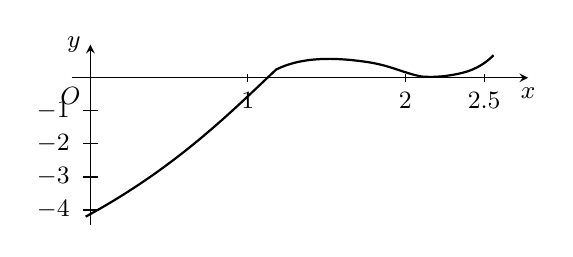
\begin{tikzpicture}[>=stealth,font=\small,x=2.0cm,y=0.42cm]
  \draw[->] (-0.12,0) -- (2.78,0) node[below] {$x$};
  \draw[->] (0,-4.45) -- (0,1.0) node[left] {$y$};
  \node[below left] at (0,0) {$O$};
  \draw[thick] (-0.03,-4.2)
    .. controls (0.55,-2.7) and (0.9,-1.0) .. (1.18,0.25)
    .. controls (1.32,0.58) and (1.5,0.64) .. (1.72,0.5)
    .. controls (1.9,0.4) and (1.98,0.15) .. (2.1,0.04)
    .. controls (2.2,-0.01) and (2.32,0.08) .. (2.4,0.2)
    .. controls (2.48,0.34) and (2.52,0.5) .. (2.56,0.68);
  \foreach \y/\l in {-1/-1,-2/-2,-3/-3,-4/-4}{
    \draw (0.05,\y) -- (-0.05,\y);
    \node[left] at (-0.07,\y) {$\l$};
  }
  \foreach \x/\l in {1/1,2/2,2.5/2.5}{
    \draw (\x,0.12) -- (\x,-0.12);
    \node[below] at (\x,-0.16) {$\l$};
  }
\end{tikzpicture}
\caption{}\label{fig:3.5.2}
\end{figure}

\begin{theorem}\label{thm:3.5.7}
设 $f$ 在区间 $I$ 上连续, 且只有惟一的极值点 $x_{0}$.

(1) 如果 $x_{0}$ 为 $f$ 的极大值点, 则 $x_{0}$ 为 $f$ 的惟一的最大值点;

(2) 如果 $x_{0}$ 为 $f$ 的极小值点, 则 $x_{0}$ 为 $f$ 的惟一的最小值点.
\end{theorem}

\begin{proof}
(1) (反证) 假设有 $x_{1}\neq x_{0}$, $x_{1}\in I$, 使 $f(x_{1})\geqslant f(x_{0})$, 不妨设 $x_{1}>x_{0}$. 由于 $f$ 在 $[x_{0},x_{1}]$ 上连续, 则它必有最小值. 因为 $x_{0}$ 为 $f$ 的极大值, 故 $\exists\delta>0$, 使得
\[
f(x)\leqslant f(x_{0}),\quad\forall x\in[x_{0},x_{0}+\delta),
\]
则必有 $x'\in(x_{0},x_{0}+\delta)$, 使 $f(x')<f(x_{0})$ (否则 $f(x)\equiv f(x_{0})$, $\forall x\in(x_{0},x_{0}+\delta)$, 从而 $(x_{0},x_{0}+\delta)$ 中任何点均为 $f$ 的极值点, 这与只有惟一的极值点 $x_{0}$ 相矛盾). 由以上讨论知, $x_{0}$ 与 $x_{1}$ 均不为 $f$ 在 $[x_{0},x_{1}]$ 中的最小值点. 其最小值点 $\xi\in(x_{0},x_{1})$, 当然 $\xi$ 为 $f$ 的极小值点, 这与 $x_{0}$ 为 $f$ 的惟一的极值点相矛盾.

(2) 可类似(1)证明, 或用 $-f$ 代替 $f$ 即可证得.
\end{proof}

\begin{example}\label{ex:3.5.11}
设 $m>0$, $n>0$, 则当 $0\leqslant x\leqslant a$ 时, 有
\[
x^{m}(a-x)^{n}\leqslant\frac{m^{m}n^{n}}{(m+n)^{m+n}}a^{m+n}.
\]
\end{example}

\begin{proof}
设 $f(x)=x^{m}(a-x)^{n}$, $0\leqslant x\leqslant a$, 则 $f(x)\geqslant 0$, 且
\[
\begin{aligned}
f'(x)&=mx^{m-1}(a-x)^{n}-nx^{m}(a-x)^{n-1}\\
&=x^{m-1}(a-x)^{n-1}[m(a-x)-nx]\\
&=x^{m-1}(a-x)^{n-1}[ma-(m+n)x]
\left\{
\begin{aligned}
&>0,\ 0\leqslant x<\frac{ma}{m+n},\quad f\ \text{单调增},\\
&=0,\ x=\frac{ma}{m+n},\quad f\ \text{取最大值},\\
&<0,\ \frac{ma}{m+n}<x\leqslant a,\quad f\ \text{单调减}.
\end{aligned}
\right.
\end{aligned}
\]
于是,
\[
\begin{aligned}
x^{m}(a-x)^{n}&=f(x)\leqslant f\Big(\frac{ma}{m+n}\Big)\\
&=\Big(\frac{ma}{m+n}\Big)^{m}\Big(a-\frac{ma}{m+n}\Big)^{n}\\
&=\frac{m^{m}}{(m+n)^{m}}\,\frac{n^{n}}{(m+n)^{n}}\,a^{m+n}\\
&=\frac{m^{n}n^{n}}{(m+n)^{m+n}}\,a^{m+n}.
\end{aligned}
\]
\end{proof}

\begin{example}\label{ex:3.5.12}
$1$, $\sqrt{2}=2^{\frac{1}{2}}$, $\sqrt[3]{3}=3^{\frac{1}{3}}$, $\cdots$, $\sqrt[n]{n}=n^{\frac{1}{n}}$, $\cdots$ 中哪一项最大.
\end{example}

\begin{solution}
令 $f(x)=x^{\frac{1}{x}}$, $x>0$, 则
\[
\begin{aligned}
f'(x)&=\big(\mathrm{e}^{\frac{1}{x}\ln x}\big)'=\mathrm{e}^{\frac{1}{x}\ln x}\Big(\frac{-1}{x^{2}}\ln x+\frac{1}{x}\cdot\frac{1}{x}\Big)\\
&=x^{\frac{1}{x}-2}(1-\ln x)
\left\{
\begin{aligned}
&>0,\quad 0<x<\mathrm{e},\ f\ \text{严格增},\\
&=0,\quad x=\mathrm{e},\ f\ \text{达最大值},\\
&<0,\quad x>\mathrm{e},\ f\ \text{严格减}.
\end{aligned}
\right.
\end{aligned}
\]
\[
\lim_{x\to 0^{+}}x^{\frac{1}{x}}=\lim_{x\to 0^{+}}\mathrm{e}^{\frac{1}{x}\ln x}=0,
\]
\[
\lim_{x\to+\infty}x^{\frac{1}{x}}=\mathrm{e}^{\lim\limits_{x\to+\infty}\frac{\ln x}{x}}=\mathrm{e}^{0}=1.
\]
由图~\ref{fig:3.5.3} 知, $\max\limits_{n\in\mathbb{N}}\sqrt[n]{n}=\max\limits_{n\in\mathbb{N}}n^{\frac{1}{n}}=\max\{\sqrt{2},\sqrt[3]{3}\}$, 所以 $\sqrt[3]{3}$ 为最大项.
\end{solution}

\begin{figure}[htbp]
\centering
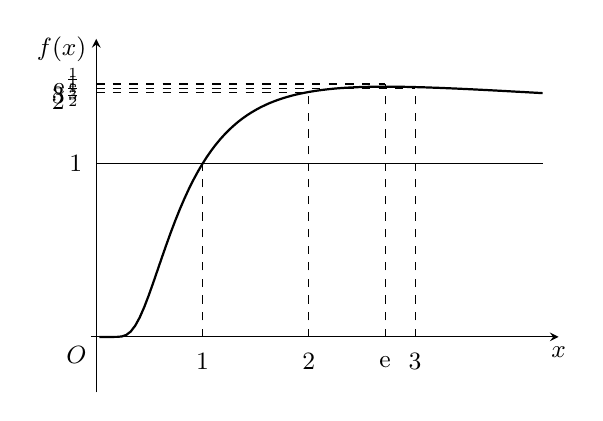
\begin{tikzpicture}[>=stealth,font=\small,x=1.35cm,y=2.2cm]
  \draw[->] (-0.05,0) -- (4.35,0) node[below] {$x$};
  \draw[->] (0,-0.32) -- (0,1.72);
  \node[left] at (0,1.66) {$f(x)$};
  \node[below left] at (0,0) {$O$};
  \draw (0,1) -- (4.2,1);
  \draw[thick] plot[domain=0.03:4.2,samples=100] (\x,{exp(ln(\x)/\x)});
  \draw[dashed] (1,0) -- (1,1);
  \draw[dashed] (2,0) -- (2,1.41);
  \draw[dashed] (2.71828,0) -- (2.71828,1.46);
  \draw[dashed] (3,0) -- (3,1.435);
  \draw[dashed] (0,1.41) -- (2,1.41);
  \draw[dashed] (0,1.46) -- (2.71828,1.46);
  \draw[dashed] (0,1.435) -- (3,1.435);
  \node[left] at (-0.04,1) {$1$};
  \node[left] at (-0.04,1.385) {$2^{\frac{1}{2}}$};
  \node[left] at (-0.04,1.425) {$3^{\frac{1}{3}}$};
  \node[left] at (-0.04,1.475) {$\mathrm{e}^{\frac{1}{\mathrm{e}}}$};
  \foreach \x/\l in {1/1,2/2,3/3}{
    \node[below] at (\x,-0.04) {$\l$};
  }
  \node[below] at (2.71828,-0.06) {$\mathrm{e}$};
\end{tikzpicture}
\caption{}\label{fig:3.5.3}
\end{figure}

\begin{example}\label{ex:3.5.13}
有长方形纸板, 长 8cm, 宽 5cm, 将四角各剪去大小相同的小正方形, 制成无盖纸盒. 问小正方形的边长为多少时, 盒子的容积最大.
\end{example}

\begin{solution}
设剪去的小正方形边长为 $x$, 则 $0<x<\frac{5}{2}$ (如图~\ref{fig:3.5.4} 所示). 纸盒容积为
\[
V=x(8-2x)(5-2x)=4x^{3}-26x^{2}+40x,
\]
\[
V'=12x^{2}-52x+40=4(3x-10)(x-1)
\]
所以, 在 $\left(0,\frac{5}{2}\right)$ 中 $V$ 的驻点为 1. 由
\[
V(0)=0,\ V(1)=18,\ V\Big(\frac{5}{2}\Big)=0
\]
知, 当 $x=1$(cm) 时, 容积 $V(1)=18$(cm$^{3}$) 为最大.
\end{solution}

\begin{figure}[htbp]
\centering
\begin{tikzpicture}[>=stealth,font=\small,scale=0.62]
  \draw[thick] (0,0) rectangle (8,5);
  \fill[pattern=north east lines] (0,0) rectangle (0.85,0.85);
  \fill[pattern=north east lines] (7.15,0) rectangle (8,0.85);
  \fill[pattern=north east lines] (0,4.15) rectangle (0.85,5);
  \fill[pattern=north east lines] (7.15,4.15) rectangle (8,5);
  \draw[decorate,decoration={brace,amplitude=4pt}] (0,5.15) -- (0.85,5.15);
  \node[above] at (0.42,5.2) {$x$};
  \draw[decorate,decoration={brace,amplitude=5pt}] (8.2,0) -- (8.2,5);
  \node[right,rotate=90] at (8.55,2.5) {$5\mathrm{cm}$};
  \draw[decorate,decoration={brace,amplitude=5pt,mirror}] (0,-0.22) -- (8,-0.22);
  \node[below] at (4,-0.34) {$8\mathrm{cm}$};
\end{tikzpicture}
\caption{}\label{fig:3.5.4}
\end{figure}

\begin{example}\label{ex:3.5.14}
设 $A$ 为铁路上一站, 从 $A$ 运原料到工厂 $C$, $C$ 距铁路的垂直距离为 $BC=20$km, $B$ 距 $A$ 的距离 $AB=150$km. 现欲在 $AB$ 之间找一点 $D$, 修公路与 $C$ 连接 (见图~\ref{fig:3.5.5}). 已知铁路运输与公路运输费用之比为 $3:5$. 问: $D$ 修在何处才能使运费最省.
\end{example}

\begin{solution}
设公路运费为 5, 则铁路运费为 3, 置 $D$ 于离 $B$ $x$ (单位: km) 处, 则运费
\[
y=f(x)=3(150-x)+5\sqrt{x^{2}+20^{2}},
\]
\[
0=f'(x)=-3+\frac{5x}{\sqrt{x^{2}+400}},
\]
\[
5x=3\sqrt{x^{2}+400},\ 25x^{2}=9x^{2}+3600,
\]
\[
16x^{2}=3600,\quad x=\pm 15.
\]
因此, 从
\[
f'(x)=-3+\frac{5x}{\sqrt{x^{2}+400}}
\left\{
\begin{aligned}
&<0,\quad x<15,\ f(x)\ \text{严格减},\\
&=0,\quad x=15,\ f(15)\ \text{为最小值},\\
&>0,\quad x>15,\ f(x)\ \text{严格增}
\end{aligned}
\right.
\]
可知 $f(x)$ 在 $x=15$ 达到最小值, 即 $D$ 应选在 $A$ 点与 $B$ 点之间距 $B$ 点 15km 处, 其运费最省 (如图~\ref{fig:3.5.5} 所示). 或者从
\[
f''(x)=\frac{1}{x^{2}+400}\left(\sqrt{x^{2}+400}-\frac{x^{2}}{\sqrt{x^{2}+400}}\right)=\frac{2000}{(x^{2}+400)^{3/2}}>0
\]
得到 $f'(x)$ 严格增, 再由 $f'(15)=0$ 推出
\[
f'(x)\left\{
\begin{aligned}
&<0,\quad x<15,\ f(x)\ \text{严格减},\\
&=0,\quad x=15,\ f(15)\ \text{为最小值},\\
&>0,\quad x>15,\ f(x)\ \text{严格增}.
\end{aligned}
\right.
\]
\end{solution}

\begin{figure}[htbp]
\centering
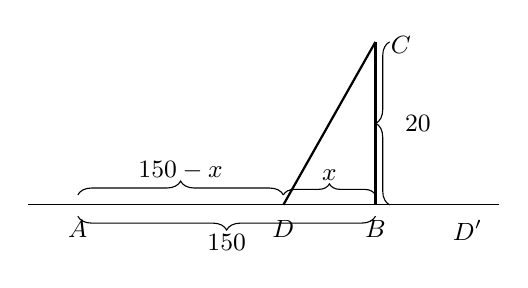
\begin{tikzpicture}[>=stealth,font=\small,scale=0.9]
  \draw (-0.35,0) -- (6.3,0);
  \draw[thick] (4.55,0) -- (4.55,2.3);
  \draw[thick] (3.25,0) -- (4.55,2.3);
  \draw[decorate,decoration={brace,amplitude=5pt}] (0.35,0.14) -- (3.25,0.14);
  \node[above] at (1.8,0.22) {$150-x$};
  \draw[decorate,decoration={brace,amplitude=4pt}] (3.25,0.14) -- (4.55,0.14);
  \node[above] at (3.9,0.2) {$x$};
  \draw[decorate,decoration={brace,amplitude=5pt}] (4.75,0) -- (4.75,2.3);
  \node[right] at (4.83,1.15) {$20$};
  \draw[decorate,decoration={brace,amplitude=5pt,mirror}] (0.35,-0.16) -- (4.55,-0.16);
  \node[below] at (2.45,-0.28) {$150$};
  \node[below] at (0.35,-0.08) {$A$};
  \node[below] at (3.25,-0.08) {$D$};
  \node[below] at (4.55,-0.08) {$B$};
  \node[below] at (5.85,-0.08) {$D'$};
  \node[right] at (4.63,2.25) {$C$};
\end{tikzpicture}
\caption{}\label{fig:3.5.5}
\end{figure}

\begin{example}\label{ex:3.5.15}
证明: 光线的入射角 $\theta_{\text{入}}$ 等于反射角 $\theta_{\text{反}}$.
\end{example}

\begin{proof}
光线服从``最短原理'': 光线从 $(0,a)$ 经 $x$ 轴上某点 $(x,0)$ 反射到 $(b,c)$ 点 (如图~\ref{fig:3.5.6} 所示). $x$ 在何处时, 所走路程 $AB+BC$ 最短.

设
\[
L(x)=AB+BC=\sqrt{a^{2}+x^{2}}+\sqrt{(b-x)^{2}+c^{2}}
\]
则
\[
L'(x)=\frac{x}{\sqrt{a^{2}+x^{2}}}-\frac{b-x}{\sqrt{(b-x)^{2}+c^{2}}},\quad 0\leqslant x\leqslant b,
\]
\[
\begin{aligned}
L''(x)&=\frac{1}{\sqrt{a^{2}+x^{2}}}-\frac{x^{2}}{\sqrt{(a^{2}+x^{2})^{3/2}}}+\frac{1}{\sqrt{(b-x)^{2}+c^{2}}}\\
&\quad-\frac{(b-x)^{2}}{\left[(b-x)^{2}+c^{2}\right]^{3/2}}\\
&=\frac{a^{2}+x^{2}-x^{2}}{(a^{2}+x^{2})^{3/2}}+\frac{(b-x)^{2}+c^{2}-(b-x)^{2}}{\left[(b-x)^{2}+c^{2}\right]^{3/2}}\\
&=\frac{a^{2}}{(a^{2}+x^{2})^{3/2}}+\frac{c^{2}}{\left[(b-x)^{2}+c^{2}\right]^{3/2}}>0.
\end{aligned}
\]
从而 $L'(x)$ 严格增, 且 $L(x)$ 在驻点 $\left(\frac{x}{\sqrt{a^{2}+x^{2}}}=\frac{b-x}{\sqrt{(b-x)^{2}+c^{2}}}\Longleftrightarrow\frac{a^{2}}{x^{2}}=\frac{c^{2}}{(b-x)^{2}}\Longleftrightarrow x=\frac{ab}{a+c}\right)$ 处达到最小值. 此时, $\triangle AOB\sim\triangle CDB$, 即 $\theta_{\text{入}}=\theta_{\text{反}}$.
\end{proof}

\begin{figure}[htbp]
\centering
\begin{tikzpicture}[>=stealth,font=\small,scale=1.0]
  \draw[->] (-0.1,0) -- (3.4,0) node[below] {$x$};
  \draw[->] (0,-0.12) -- (0,2.75);
  \node[left] at (0,2.68) {$y$};
  \node[below left] at (0,0) {$O$};
  \draw (2.95,0) -- (2.95,2.35);
  \draw[->] (0,2.0) -- (1.05,0);
  \draw[->] (1.05,0) -- (2.95,2.35);
  \draw[dashed] (1.05,0) -- (1.05,2.2);
  \draw (1.05,0.5) arc[start angle=90,end angle=117.7,radius=0.5];
  \draw (1.05,0.62) arc[start angle=50.3,end angle=90,radius=0.62];
  \node at (0.66,0.66) {$\theta_{\text{入}}$};
  \node at (1.5,0.86) {$\theta_{\text{反}}$};
  \node[above right] at (0,1.95) {$A(0,a)$};
  \node[below] at (1.05,-0.1) {$B(x,0)$};
  \node[below] at (2.95,-0.1) {$D(b,0)$};
  \node[right] at (2.99,2.35) {$C(b,c)$};
\end{tikzpicture}
\caption{}\label{fig:3.5.6}
\end{figure}

\begin{example}\label{ex:3.5.16}
炼油厂要修建容量为 $V_{0}$ 的贮油罐. 问: 此罐的底面直径与高之比为多少时, 用料量最省即表面积最小.
\end{example}

\begin{solution}
设油罐底面半径为 $r$, 高为 $h$, 则
\[
S=2\pi rh+2\pi r^{2}
\]
\[
V_{0}=\pi r^{2}h,\quad h=\frac{V_{0}}{\pi r^{2}},\quad r>0.
\]
于是,
\[
S=2\pi r\cdot\frac{V_{0}}{\pi r^{2}}+2\pi r^{2}=\frac{2V_{0}}{r}+2\pi r^{2},\quad r>0.
\]
\[
\begin{aligned}
S'&=-\frac{2V_{0}}{r^{2}}+4\pi r\\
&=\frac{2}{r^{2}}(2\pi r^{3}-V_{0})
\left\{
\begin{aligned}
&<0,\quad 0<r<\sqrt[3]{\frac{V_{0}}{2\pi}},\ S(r)\ \text{严格减},\\
&=0,\quad r=\sqrt[3]{\frac{V_{0}}{2\pi}},\ S\Big(\sqrt[3]{\frac{V_{0}}{2\pi}}\Big)\ \text{为最小值},\\
&>0,\quad r>\sqrt[3]{\frac{V_{0}}{2\pi}},\ S(r)\ \text{严格增},
\end{aligned}
\right.
\end{aligned}
\]
即当 $\frac{2r}{h}=\frac{2r}{\frac{V_{0}}{\pi r^{2}}}=\frac{2\pi r^{3}}{V_{0}}=\frac{2\pi\cdot\frac{V_{0}}{2\pi}}{V_{0}}=1$ 时, 表面积最省.
\end{solution}

\begin{exblock}{练习题 3.5}
  \item 确定下列函数的单调区间:
  \begin{enumerate}[label=(\arabic*)]
    \item $f(x)=3x-x^{2}$;
    \item $f(x)=2x^{2}-\ln x$;
    \item $f(x)=\sqrt{2x-x^{2}}$;
    \item $f(x)=\frac{x^{2}-1}{x}$;
    \item $f(x)=\arctan x-x$.
  \end{enumerate}

  \item 应用函数的单调性证明下列不等式:
  \begin{enumerate}[label=(\arabic*)]
    \item $\tan x>x-\frac{x^{3}}{3}$, $x\in\left(0,\frac{\pi}{3}\right)$;
    \item $\frac{2x}{\pi}<\sin x<x$, $x\in\left(0,\frac{\pi}{2}\right)$;
    \item $x-\frac{x^{2}}{2}<\ln(1+x)<x-\frac{x^{2}}{2(1+x)}$;
    \item $x(x-\arctan x)>0$, $x\neq 0$;
    \item $\ln(1+x)>\frac{\arctan x}{1+x}$, $x>0$.
  \end{enumerate}

  \item 设 $a,b>0$. 证明: 方程 $x^{3}+ax+b=0$ 不存在正根.

  \item 证明: $\frac{\tan x}{x}>\frac{x}{\sin x}$, $x\in\left(0,\frac{\pi}{2}\right)$.

  \item 设函数 $f$ 与 $g$ 在区间 $[a,+\infty)$ 上连续可导, 且当 $x>a$ 时, $|f'(x)|\leqslant g'(x)$. 证明: 当 $x\geqslant a$ 时,
  \[
  |f(x)-f(a)|\leqslant g(x)-g(a).
\]

  \item 设函数 $y=f(x)$ 在点 $x$ 处 3 阶可导, 且 $f'(x)\neq 0$. 证明: $f(x)$ 严格增或严格减, 从而存在反函数 $x=f^{-1}(y)$. 试用 $f'(x)$, $f''(x)$ 及 $f'''(x)$ 表示 $(f^{-1})''(y)$.

  \item 证明:
  (1) 方程 $x^{3}-3x+c=0$ ($c$ 为常数) 在区间 $[0,1]$ 内不可能有两个不同的实根.

  (2) 方程 $x^{n}+px+q=0$ ($n\in\mathbb{N}$, $p,q\in\mathbb{R}$) 当 $n$ 为偶数时至多有 2 个实根; 当 $n$ 为奇数时至多有 3 个实根.

  \item 设函数 $f$ 在 $[a,b]$ 上可导. 证明:
  (1) 若 $f'(x)\geqslant m$, 则 $f(x)\geqslant f(a)+m(x-a)$, $\forall x\in[a,b]$;

  (2) 若 $|f'(x)|\leqslant M$, 则 $|f(x)-f(a)|\leqslant M(x-a)$, $\forall x\in[a,b]$.

  \item 求下列函数的极值:
  \begin{enumerate}[label=(\arabic*)]
    \item $f(x)=2x^{3}-x^{4}$;
    \item $f(x)=\frac{2x}{1+x^{2}}$;
    \item $f(x)=\frac{(\ln x)^{2}}{x}$;
    \item $f(x)=\arctan x-\frac{1}{2}\ln(1+x^{2})$;
    \item $f(x)=|x(x^{2}-1)|$;
    \item $f(x)=(x-1)^{2}(x+1)^{3}$;
    \item $f(x)=\frac{x(x^{2}+1)}{x^{4}-x^{2}+1}$.
  \end{enumerate}

  \item 设
  \[
  f(x)=\left\{
  \begin{aligned}
  &x^{4}\sin^{2}\frac{1}{x},\quad x\neq 0,\\
  &0,\quad x=0.
  \end{aligned}
  \right.
\]
  (1) 证明: $x=0$ 为 $f$ 的极小值点, 也是最小值点;

  (2) 说明 $f$ 的极小值点 $x=0$ 处是否满足极值的充分条件一或充分条件二.

  \item 求下列函数在给定区间上的最大与最小值:
  \begin{enumerate}[label=(\arabic*)]
    \item $f(x)=x^{4}-2x^{2}+5$, $|x|\leqslant 2$;
    \item $f(x)=x^{5}-5x^{4}+5x^{3}+1$, $x\in[-1,2]$;
    \item $f(x)=x\ln x$, $x>0$;
    \item $f(x)=\sqrt{x}\ln x$, $x>0$;
    \item $f(x)=x^{2}-3x+2$, $x\in\mathbb{R}$;
    \item $f(x)=|x^{2}-3x+2|$, $|x|\leqslant 10$;
    \item $f(x)=2\tan x-\tan^{2}x$, $x\in\left[0,\frac{\pi}{2}\right)$;
    \item $f(x)=\arctan\frac{1-x}{1+x}$, $0\leqslant x\leqslant 1$.
  \end{enumerate}

  \item 设函数 $f$ 在点 $x_{0}$ 处有 $f'_{+}(x_{0})<0\,(>0)$, $f'_{-}(x_{0})>0\,(<0)$, 则 $x_{0}$ 为 $f$ 极大(小)值点.

  \item 证明: 当 $x>0$ 且 $x\neq 1$ 时, 有 $(1-x)\big(x^{2}\mathrm{e}^{\frac{1}{x}}-\mathrm{e}^{x}\big)>0$ (提示: 考察 $\varphi(x)=2\ln x+\frac{1}{x}-x$).

  \item 求一正数 $x$, 使它与其倒数之和 $f(x)=x+\frac{1}{x}$ 最小.

  \item 证明: (1) 周长为 $l$ 的矩形中, 以正方形所围面积最大; (2) 面积为定值 $S$ 的矩形中, 以正方形的边长为最小.

  \item 设用某仪器进行测量时, 读得 $n$ 次实验数据为 $a_{1},a_{2},\cdots,a_{n}$. 问以怎样的数值 $x$ 表达所要测量的真值, 才能使它与这 $n$ 个数之差的平方和为最小 (提示: 即证 $f(x)=\sum\limits_{i=1}^{n}(x-a_{i})^{2}$ 的最小值为 $\bar{x}=\frac{a_{1}+a_{2}+\cdots+a_{n}}{n}$).

  \item 内接于椭圆 $\frac{x^{2}}{a^{2}}+\frac{y^{2}}{b^{2}}=1$, 边平行于坐标轴的矩形, 何时面积最大.

  \item 从半径为 $R$ 的圆纸片上剪去一个扇形, 做成一个圆锥形的漏斗. 如何选取扇形的顶角, 可使漏斗的容积最大.

  \item 设 $0<a<b\leqslant 2a$, 在区间 $[a,b]$ 上讨论双曲线 $xy=1$. 在该曲线每一点上作切线, 它与横轴及两平行直线 $x=a$, $x=b$ 围成一个梯形. 问这切线位于何处, 才能使梯形有最大面积.

  \item 在抛物线 $y^{2}=2px$ 上哪一点的法线被抛物线所截之线段为最短.

  \item 有一个无盖的圆柱形容器, 当给定体积为 $V_{0}$ 时, 要使容器的表面积为最小, 问底的半径与容器高的比例为多大.

  \item 要将货物从运河边上 $A$ 城运往与运河相距 $a$ (单位: km) 的 $B$ 城, 轮船运费的单价是 $\alpha$ 元/km, 火车运费的单价是 $\beta$ 元/km ($\beta>\alpha$). 试求运河边上的一点 $M$, 修建铁路 $MB$, 使总运费最省.

  \item 重量为 $W$ 的物体放在一粗糙的平面上, 施加一力克服摩擦, 使之在平面上滑动, 其摩擦系数为 $\mu$, 问该力应与水平成何角度, 方可使用力最小?

  \item 设 $f(x)=a\ln x+bx^{2}+x$ 在 $x_{1}=1$, $x_{2}=2$ 处都取得极值, 试求 $a$ 与 $b$; 并问此时 $f$ 在 $x_{1}$ 与 $x_{2}$ 是取得极大值还是极小值.

  \item 证明: 定圆内接正 $n$ 边形面积随 $n$ 的增加而增加.

  \item 讨论函数
  \[
  f(x)=\left\{
  \begin{aligned}
  &\frac{x}{2}+x^{2}\sin\frac{1}{x},\quad x\neq 0,\\
  &0,\quad x=0.
  \end{aligned}
  \right.
\]
  (1) 在 $x=0$ 点是否可导.

  (2) 是否存在 $x=0$ 的一个开邻域, 使 $f$ 在该开邻域内单调.

  \item 设 $k>0$. 试问: $k$ 为何值时, 方程 $\arctan x-kx=0$ 有正实根.
\end{exblock}

\begin{exblock}{思考题 3.5}
  \item 设 $0<b<a$. 证明:
  \[
  \frac{a-b}{\sqrt{1+a^{2}}\sqrt{1+b^{2}}}<\arctan a-\arctan b<a-b,\quad\text{其中 } 0<b<a.
\]

  \item 证明下列不等式:
  (1) 当 $0<x_{1}<x_{2}<\frac{\pi}{2}$ 时, 有
  \[
  \frac{\tan x_{2}}{\tan x_{1}}>\frac{x_{2}}{x_{1}};
\]

  (2) 当 $x,y>0$ 且 $\beta>\alpha>0$ 时, 有
  \[
  (x^{\alpha}+y^{\alpha})^{\frac{1}{\alpha}}>(x^{\beta}+y^{\beta})^{\frac{1}{\beta}};
\]

  (3) 设 $p\geqslant 2$, 当 $x\in[0,1]$ 时, 有
  \[
  \left(\frac{1+x}{2}\right)^{p}+\left(\frac{1-x}{2}\right)^{p}\leqslant\frac{1}{2}(1+x^{p}).
\]

  \item 设函数 $f$ 在区间 $[0,+\infty)$ 上可导, $f(0)=0$ 且 $f'$ 严格增. 证明: $\frac{f(x)}{x}$ 在 $(0,+\infty)$ 上也严格增.

  \item 设求出使得不等式 $a^{x}\geqslant x^{a}$ ($x>0$) 成立的一切正数 $a$ (提示: 考察函数 $f(x)=\frac{\ln x}{x}$).

  \item 设 $f$ 在 $[a,+\infty)$ 上 2 阶可导, 且 $f(a)>0$, $f'(a)<0$, 当 $x>a$ 时, $f''(x)\leqslant 0$. 证明: 方程 $f(x)=0$ 在 $(a,+\infty)$ 内有且仅有一根.
\end{exblock}

% ==================================================================
%  徐森林、薛春华《数学分析》（第一册）
%  \S3.6  应用导数研究函数之二: 凹凸性、图形
% ==================================================================
%  源：原书印刷页 221-241（PDF 物理页 227-247）
%  底本：PaddleOCR-VL-1.6 + 高清影印比对校订
%  规范：全西文半角标点；单一落盘出口 _texout.py
% ==================================================================
\section{应用导数研究函数之二: 凹凸性、图形}\label{sec:3.6}

继 3.5 节, 应用 Lagrange 中值定理来研究函数的凹凸性.

\begin{definition}\label{def:3.6.1}
设 $f$ 为区间 $I$ 上的函数. 如果 $\forall x_{1},x_{2}\in I$, $\forall \lambda\in (0,1)$, 总有
\[
f(\lambda x_{1}+(1-\lambda)x_{2})\leqslant \lambda f(x_{1})+(1-\lambda)f(x_{2}),
\]
则称 $f$ 在 $I$ 上为\textbf{凸函数}(或\textbf{下凸函数}).

如果上述不等式中“$\leqslant$”改为“$<$”, 则称 $f$ 在 $I$ 上为\textbf{严格凸函数}(或\textbf{严格下凸函数}).

如果 $\forall x_{1},x_{2}\in I$, $\forall \lambda\in (0,1)$, 总有
\[
f(\lambda x_{1}+(1-\lambda)x_{2})\geqslant \lambda f(x_{1})+(1-\lambda)f(x_{2}),
\]
则称 $f$ 在 $I$ 上为\textbf{凹函数}.

如果上述不等式中“$\geqslant$”改为“$>$”, 则称 $f$ 在 $I$ 上为\textbf{严格凹函数}.
\end{definition}

从几何上看, 凸(凹)函数 $y=f(x)$ ($x\in I$) 的图形上的任何不同的两点间的曲线段完全落在连接该两点的直线段(称为曲线过这两点的\textbf{弦})的下(上)方、严格凸(凹)函数 $y=f(x)$ ($x\in I$) 的图形上的任何不同的两点间的曲线段完全严格落在该两点的弦的下(上)方(如图~\ref{fig:3.6.1}、图~\ref{fig:3.6.2} 所示, 其中 $x=\lambda x_{1}+(1-\lambda)x_{2}$).

\begin{figure}[htbp]
\centering
\begin{minipage}[t]{0.49\textwidth}
\centering
\begin{tikzpicture}[scale=0.72, >=Stealth, font=\small, baseline=(current bounding box.north)]
  \draw[->] (-0.3,0) -- (4.2,0) node[below] {$x$};
  \draw[->] (0,-0.3) -- (0,3.6) node[left] {$y$};
  \node[below left] at (0,0) {$O$};
  
  \draw[very thick] (0.5,0.7) to[out=10, in=250] (3.8,3.3) node[right] {$y=f(x)$};
  
  \def\xone{0.8}
  \def\xtwo{3.4}
  \def\xmid{2.2}
  
  \coordinate (P1) at (\xone, 0.74);
  \coordinate (P2) at (\xtwo, 2.6);
  \path (P1) -- (P2) coordinate[pos=0.538] (S);
  \coordinate (C) at (\xmid, 1.25);
  
  \draw[thick] (P1) -- (P2);
  
  \draw[dashed] (\xone,0) node[below] {$x_1$} -- (P1) -- (0,0.74) node[left] {$f(x_1)$};
  \draw[dashed] (\xtwo,0) node[below] {$x_2$} -- (P2) -- (0,2.6) node[left] {$f(x_2)$};
  \draw[dashed] (\xmid,0) node[below] {$x$} -- (S) -- (0,{1.87}) node[above left=-2pt] {\scriptsize $\lambda f(x_1)+(1-\lambda)f(x_2)$};
  \draw[dashed] (C) -- (0,1.25) node[left] {$f(x)$};
  
  \fill (P1) circle (1.5pt);
  \fill (P2) circle (1.5pt);
  \fill (S) circle (1.5pt);
  \fill (C) circle (1.5pt);
\end{tikzpicture}
\caption{凸函数}\label{fig:3.6.1}
\end{minipage}
\hfill
\begin{minipage}[t]{0.49\textwidth}
\centering
\begin{tikzpicture}[scale=0.72, >=Stealth, font=\small, baseline=(current bounding box.north)]
  \draw[->] (-0.3,0) -- (4.2,0) node[below] {$x$};
  \draw[->] (0,-0.3) -- (0,3.6) node[left] {$y$};
  \node[below left] at (0,0) {$O$};
  
  \draw[very thick] (0.5,0.7) to[out=70, in=190] (3.8,3.1) node[right] {$y=f(x)$};
  
  \def\xone{0.8}
  \def\xtwo{3.4}
  \def\xmid{2.2}
  
  \coordinate (P1) at (\xone, 1.35);
  \coordinate (P2) at (\xtwo, 2.95);
  \path (P1) -- (P2) coordinate[pos=0.538] (S);
  \coordinate (C) at (\xmid, 2.75);
  
  \draw[thick] (P1) -- (P2);
  
  \draw[dashed] (\xone,0) node[below] {$x_1$} -- (P1) -- (0,1.35) node[left] {$f(x_1)$};
  \draw[dashed] (\xtwo,0) node[below] {$x_2$} -- (P2) -- (0,2.95) node[left] {$f(x_2)$};
  \draw[dashed] (\xmid,0) node[below] {$x$} -- (C) -- (0,2.75) node[left] {$f(x)$};
  \draw[dashed] (S) -- (0,{2.21}) node[above left=-2pt] {\scriptsize $\lambda f(x_1)+(1-\lambda)f(x_2)$};
  
  \fill (P1) circle (1.5pt);
  \fill (P2) circle (1.5pt);
  \fill (S) circle (1.5pt);
  \fill (C) circle (1.5pt);
\end{tikzpicture}
\caption{凹函数}\label{fig:3.6.2}
\end{minipage}
\end{figure}

显然, $f$ 在区间 $I$ 上为(严格)凸(凹)函数 $\Longleftrightarrow -f$ 在区间 $I$ 上为(严格)凹(凸)函数. 因此, 凡对(严格)凸函数成立的命题, (严格)凹函数也成立相应的命题. 这可以类似(严格)凸函数的证明, 或者用 $-f$ 代替 $f$ 并应用(严格)凸函数的结论推得. 因此, 今后只须讨论(严格)凸函数的性质即可.

\begin{theorem}\label{thm:3.6.1}
$f$ 在区间 $I$ 中为凸函数 $\Longleftrightarrow \forall x_{1},x_{2},x_{3}\in I$, $x_{1}<x_{2}<x_{3}$, 下面不等式
\[
\frac{f(x_{2})-f(x_{1})}{x_{2}-x_{1}}\leqslant\frac{f(x_{3})-f(x_{1})}{x_{3}-x_{1}}\leqslant\frac{f(x_{3})-f(x_{2})}{x_{3}-x_{2}}
\]
中任何两个组成的不等式成立(如图~\ref{fig:3.6.3} 所示).
\end{theorem}

\begin{figure}[htbp]
\centering
\begin{tikzpicture}[scale=0.9, >=Stealth, font=\small]
  \draw[->] (-0.3,0) -- (5.0,0) node[below] {$x$};
  \draw[->] (0,-0.3) -- (0,4.2) node[left] {$y$};
  \node[below left] at (0,0) {$O$};
  
  \draw[very thick] (0.6,0.8) to[out=10, in=250] (4.2,3.8);
  
  \coordinate (P1) at (0.9, 0.95);
  \coordinate (P2) at (2.4, 1.6);
  \coordinate (P3) at (3.8, 3.4);
  
  \draw[thick] (P1) -- (P2) -- (P3) -- cycle;
  
  \draw[dashed] (P1) -- (0.9,0) node[below] {$x_1$};
  \draw[dashed] (P2) -- (2.4,0) node[below=1pt] {$x_2$};
  \node[below=14pt, align=center] at (2.4,0) {\scriptsize $x_2=\lambda x_1+(1-\lambda)x_3$\\[
1pt] \scriptsize $\lambda = \frac{x_3-x_2}{x_3-x_1}$};
  \draw[dashed] (P3) -- (3.8,0) node[below] {$x_3$};
  \fill (P1) circle (1.5pt) node[below left=-1pt] {$P_1(x_1,f(x_1))$};
  \fill (P2) circle (1.5pt) node[below right=-2pt] {$P_2(x_2,f(x_2))$};
  \fill (P3) circle (1.5pt) node[right=1pt] {$P_3(x_3,f(x_3))$};
\end{tikzpicture}
\caption{三条弦的斜率}\label{fig:3.6.3}
\end{figure}
\begin{proof}
(1) $f$ 在区间 $I$ 上为凸函数
\begin{align*}
&\Longleftrightarrow f(x_{2})=f\left(\frac{x_{3}-x_{2}}{x_{3}-x_{1}}x_{1}+\frac{x_{2}-x_{1}}{x_{3}-x_{1}}x_{3}\right)\\
&\quad\leqslant \frac{x_{3}-x_{2}}{x_{3}-x_{1}}f(x_{1})+\frac{x_{2}-x_{1}}{x_{3}-x_{1}}f(x_{3})\\
&\Longleftrightarrow f(x_{3})-f(x_{2})\geqslant \frac{x_{3}-x_{1}-x_{2}+x_{1}}{x_{3}-x_{1}}f(x_{3})-\frac{x_{3}-x_{2}}{x_{3}-x_{1}}f(x_{1})\\
&\quad=\frac{x_{3}-x_{2}}{x_{3}-x_{1}}f(x_{3})-\frac{x_{3}-x_{2}}{x_{3}-x_{1}}f(x_{1})\\
&\quad=\frac{x_{3}-x_{2}}{x_{3}-x_{1}}[f(x_{3})-f(x_{1})]\\
&\Longleftrightarrow \frac{f(x_{3})-f(x_{1})}{x_{3}-x_{1}}\leqslant \frac{f(x_{3})-f(x_{2})}{x_{3}-x_{2}}.
\end{align*}
(2) $f$ 在区间 $I$ 上为凸函数
\begin{align*}
&\Longleftrightarrow f(x_{2})-f(x_{1})\leqslant \frac{x_{3}-x_{2}-x_{3}+x_{1}}{x_{3}-x_{1}}f(x_{1})+\frac{x_{2}-x_{1}}{x_{3}-x_{1}}f(x_{3})\\
&\quad=-\frac{x_{2}-x_{1}}{x_{3}-x_{1}}f(x_{1})+\frac{x_{2}-x_{1}}{x_{3}-x_{1}}f(x_{3})\\
&\quad=\frac{x_{2}-x_{1}}{x_{3}-x_{1}}[f(x_{3})-f(x_{1})]\\
&\Longleftrightarrow \frac{f(x_{2})-f(x_{1})}{x_{2}-x_{1}}\leqslant \frac{f(x_{3})-f(x_{1})}{x_{3}-x_{1}}.
\end{align*}
(3) $f$ 在区间 $I$ 上为凸函数
\begin{align*}
&\Longleftrightarrow (x_{3}-x_{1})f(x_{2})\leqslant (x_{3}-x_{2})f(x_{1})+(x_{2}-x_{1})f(x_{3})\\
&\Longleftrightarrow -(x_{3}-x_{2})f(x_{1})\leqslant (x_{2}-x_{1})f(x_{3})-(x_{3}-x_{2}+x_{2}-x_{1})f(x_{2})\\
&\Longleftrightarrow (x_{3}-x_{2})[f(x_{2})-f(x_{1})]\leqslant (x_{2}-x_{1})[f(x_{3})-f(x_{2})]\\
&\Longleftrightarrow \frac{f(x_{2})-f(x_{1})}{x_{2}-x_{1}}\leqslant \frac{f(x_{3})-f(x_{2})}{x_{3}-x_{2}}.
\end{align*}
\end{proof}
观察一下定理~\ref{thm:3.6.1} 的几何意义是有帮助的. 在图~\ref{fig:3.6.3} 中, 画出了 $y=f(x)$ 的三条弦 $P_{1}P_{2},P_{2}P_{3},P_{1}P_{3}$, 其中 $P_{i}=(x_{i},f(x_{i}))$, $i=1,2,3$. 这三条弦组成了一个三角形. 定理~\ref{thm:3.6.1} 中不等式的几何表示是
\[
\overline{P_{1}P_{2}}\ \text{的斜率}\leqslant \overline{P_{1}P_{3}}\ \text{的斜率}\leqslant \overline{P_{2}P_{3}}\ \text{的斜率}.
\]
这正表示曲线 $y=f(x)$ 的下凸状态, 几何表示便于定理~\ref{thm:3.6.1} 中不等式的记忆.

关于凸函数, 有重要的 Jensen(詹森)不等式.

\begin{theorem}[Jensen 不等式]\label{thm:3.6.2}
$f$ 在区间 $I$ 上为凸函数 $\Longleftrightarrow \forall x_{i}\in I$, $\forall \lambda_{i}>0$ ($i=1,2,\cdots,n$), $\sum_{i=1}^{n}\lambda_{i}=1$, 有
\[
f\left(\sum_{i=1}^{n}\lambda_{i}x_{i}\right)\leqslant \sum_{i=1}^{n}\lambda_{i}f(x_{i}).
\]
如果 $f$ 在区间 $I$ 上为严格凸函数, 则当上述 $x_{1},x_{2},\cdots,x_{n}\in I$ 不全相等时, 有
\[
f\left(\sum_{i=1}^{n}\lambda_{i}x_{i}\right)< \sum_{i=1}^{n}\lambda_{i}f(x_{i}).
\]
\end{theorem}

\begin{proof}
($\Longrightarrow$) 设 $f$ 在区间 $I$ 上为凸函数.

(归纳法) 当 $n=1$ 时, $\lambda_{1}=1$, $f\left(\sum_{i=1}^{1}\lambda_{i}x_{i}\right)=f(\lambda_{1}x_{1})=f(x_{1})=\sum_{i=1}^{1}\lambda_{i}f(x_{i})$;

当 $n=2$ 时, $\lambda_{1}=\lambda$, $\lambda_{2}=1-\lambda$,
\[
f\left(\sum_{i=1}^{2}\lambda_{i}x_{i}\right)=f(\lambda x_{1}+(1-\lambda)x_{2})\leqslant \lambda f(x_{1})+(1-\lambda)f(x_{2})=\sum_{i=1}^{2}\lambda_{i}f(x_{i});
\]
假设 $n=k$ 时, $\forall x_{i}\in I$, $\forall \lambda_{i}>0$ ($i=1,2,\cdots,k$), $\sum_{i=1}^{k}\lambda_{i}=1$, 有
\[
f\left(\sum_{i=1}^{k}\lambda_{i}x_{i}\right)\leqslant \sum_{i=1}^{k}\lambda_{i}f(x_{i}),
\]
则当 $n=k+1$ 时, $\forall x_{i}\in I$, $\forall \lambda_{i}>0$ ($i=1,2,\cdots,k+1$), $\sum_{i=1}^{k+1}\lambda_{i}=1$. 令 $\mu_{i}=\frac{\lambda_{i}}{1-\lambda_{k+1}}$, $i=1,2,\cdots,k$, 便有 $\mu_{i}>0$ 且 $\sum_{i=1}^{k}\mu_{i}=\sum_{i=1}^{k}\frac{\lambda_{i}}{1-\lambda_{k+1}}=\frac{1-\lambda_{k+1}}{1-\lambda_{k+1}}=1$. 于是,
\begin{align*}
f\left(\sum_{i=1}^{k+1}\lambda_{i}x_{i}\right)&=f\left((1-\lambda_{k+1})\sum_{i=1}^{k}\frac{\lambda_{i}}{1-\lambda_{k+1}}x_{i}+\lambda_{k+1}x_{k+1}\right)\\
&\leqslant (1-\lambda_{k+1})f\left(\sum_{i=1}^{k}\frac{\lambda_{i}}{1-\lambda_{k+1}}x_{i}\right)+\lambda_{k+1}f(x_{k+1}).
\end{align*}
归纳可得
\begin{align*}
f\left(\sum_{i=1}^{k+1}\lambda_{i}x_{i}\right)&\leqslant (1-\lambda_{k+1})\sum_{i=1}^{k}\frac{\lambda_{i}}{1-\lambda_{k+1}}f(x_{i})+\lambda_{k+1}f(x_{k+1})\\
&=\sum_{i=1}^{k+1}\lambda_{i}f(x_{i}).
\end{align*}

($\Longleftarrow$) 如果右边条件成立, 特别当 $n=2$ 时, $\lambda=\lambda_{1}$, $1-\lambda=1-\lambda_{1}=\lambda_{2}$, 故有
\[
f(\lambda x_{1}+(1-\lambda)x_{2})=f(\lambda_{1}x_{1}+\lambda_{2}x_{2})\leqslant \lambda_{1}f(x_{1})+\lambda_{2}f(x_{2})=\lambda f(x_{1})+(1-\lambda)f(x_{2}).
\]
这就证明了 $f$ 在区间 $I$ 上为凸函数.

关于严格凸函数情形, 当 $x_{1},x_{2},\cdots,x_{n}$ 不全相等时, 我们重新审查归纳证明. 当 $n=2$ 时, $x_{1},x_{2}$ 不全相等就是 $x_{1}\neq x_{2}$, 按定义, 严格的不等号成立. 假设 $n=k$ 时, 严格不等号成立. 再设 $x_{1},x_{2},\cdots,x_{k+1}$ 不全相等, 如果其中 $x_{1},x_{2},\cdots,x_{k}$ 不全相等, 则上述归纳法中最后的那个不等号应当是严格的; 如果 $x_{1}=\cdots=x_{k}\neq x_{k+1}$, 则 $\sum_{i=1}^{k}\mu_{i}x_{i}=x_{1}\sum_{i=1}^{k}\mu_{i}=x_{1}\neq x_{k+1}$, 此时归纳过程的第 1 个不等号是严格的. 总之, 不等式
\[
f\left(\sum_{i=1}^{n}\lambda_{i}x_{i}\right)<\sum_{i=1}^{n}\lambda_{i}f(x_{i})
\]
对一切 $n\in\mathbb{N}$ 成立.
\end{proof}

\begin{theoremp}[Jensen 不等式]\label{thm:3.6.2p}
$f$ 在区间 $I$ 上为凸函数 $\Longleftrightarrow \forall x_{i}\in I$, $\forall \beta_{i}>0$ ($i=1,2,\cdots,n$), 有
\[
f\left(\frac{\displaystyle\sum_{i=1}^{n}\beta_{i}x_{i}}{\displaystyle\sum_{i=1}^{n}\beta_{i}}\right)\leqslant\frac{\displaystyle\sum_{i=1}^{n}\beta_{i}f(x_{i})}{\displaystyle\sum_{i=1}^{n}\beta_{i}}.
\]
如果 $f$ 是严格凸的, 则当上述 $x_{1},x_{2},\cdots,x_{n}\in I$ 不全相等时有
\[
f\left(\frac{\displaystyle\sum_{i=1}^{n}\beta_{i}x_{i}}{\displaystyle\sum_{i=1}^{n}\beta_{i}}\right)<\frac{\displaystyle\sum_{i=1}^{n}\beta_{i}f(x_{i})}{\displaystyle\sum_{i=1}^{n}\beta_{i}}.
\]
\end{theoremp}

在函数 $f$ 有导函数 $f'$ 的情况下, 判断 $f$ 的凸性将变得比较容易, 因为我们有下面定理.

\begin{theorem}\label{thm:3.6.3}
设 $f$ 在区间 $I$ 上可导, 则下面三个结论等价:
\begin{enumerate}[label=(\arabic*)]
  \item $f$ 在 $I$ 上为(严格)凸函数;
  \item $f'$ 在 $I$ 上为(严格)增函数;
  \item $\forall x_{0},x\in I$, $x\neq x_{0}$, 有
  \[
  f(x)\geqslant f(x_{0})+f'(x_{0})(x-x_{0})
\]
  (或 $f(x)>f(x_{0})+f'(x_{0})(x-x_{0})$), 即 $f$ 的图形(严格)在其任一点 $(x_{0},f(x_{0}))$ 的切线的上方.
\end{enumerate}
\end{theorem}

\begin{figure}[htbp]
\centering
\begin{tikzpicture}[scale=0.9, >=Stealth, font=\small]
  \draw[->] (-0.3,0) -- (4.8,0) node[below] {$x$};
  \draw[->] (0,-0.3) -- (0,4.2) node[left] {$y$};
  \node[below left] at (0,0) {$O$};
  
  \draw[very thick] (0.8,1.2) to[out=5, in=250] (3.8,3.6);
  
  \coordinate (P1) at (1.0, 1.25);
  \coordinate (P1h) at (1.6, 1.35);
  \coordinate (P2h) at (3.1, 2.55);
  \coordinate (P2) at (3.8, 3.6);
  
  \draw[thick] (P1) -- (P2);
  \draw[dashed] (P1) -- (P1h);
  \draw[dashed] (P2h) -- (P2);
  
  \draw[dashed] (P1) -- (1.0,0) node[below] {$x_1$};
  \draw[dashed] (P1h) -- (1.6,0) node[below] {$x_1+h$};
  \draw[dashed] (P2h) -- (3.1,0) node[below] {$x_2-h$};
  \draw[dashed] (P2) -- (3.8,0) node[below] {$x_2$};
  
  \fill (P1) circle (1.5pt) node[above left=-1pt] {$(x_1,f(x_1))$};
  \fill (P1h) circle (1.5pt) node[below right=-1pt] {$(x_1+h,f(x_1+h))$};
  \fill (P2h) circle (1.5pt) node[right=1pt] {$(x_2-h,f(x_2-h))$};
  \fill (P2) circle (1.5pt) node[right=1pt] {$(x_2,f(x_2))$};
\end{tikzpicture}
\caption{割线斜率的逼近}\label{fig:3.6.4}
\end{figure}

\begin{proof}
(1) $\Longrightarrow$ (2) 设 $f$ 在 $I$ 上为凸函数, 即 $\forall x_{1},x_{2}\in I$, $x_{1}<x_{2}$, 充分小的 $h>0$, 使得 $x_{1}<x_{1}+h<x_{2}-h<x_{2}$. 根据 $f$ 的凸性及定理~\ref{thm:3.6.1}, 有(如图~\ref{fig:3.6.4} 所示)
\[
\frac{f(x_{1}+h)-f(x_{1})}{h}\leqslant\frac{f(x_{2})-f(x_{1})}{x_{2}-x_{1}}\leqslant\frac{f(x_{2})-f(x_{2}-h)}{h}.
\]
因为 $f$ 可导, 令 $h\to 0^{+}$, 得到
\[
f'(x_{1})=f'_{+}(x_{1})\leqslant\frac{f(x_{2})-f(x_{1})}{x_{2}-x_{1}}\leqslant f'_{-}(x_{2})=f'(x_{2}),
\]
所以, $f'$ 在 $I$ 上为增函数.

在 $f$ 为严格凸函数的情形时, 我们取定一点 $x^{*}\in (x_{1},x_{2})$, 从而得出
\[
f'(x_{1})\leqslant\frac{f(x^{*})-f(x_{1})}{x^{*}-x_{1}}<\frac{f(x_{2})-f(x^{*})}{x_{2}-x^{*}}\leqslant f'(x_{2}).
\]
这就得出了严格不等式 $f'(x_{1})<f'(x_{2})$, 即 $f'$ 在 $I$ 上为严格增函数.

(1) $\Longleftarrow$ (2) 设 $f'$ 在 $I$ 上为增函数. 对任何 $x_{1}<x_{2}<x_{3}$, 由 Lagrange 中值定理知, 存在 $x_{1}<\xi_{1}<x_{2}<\xi_{2}<x_{3}$, 使得
\[
\frac{f(x_{2})-f(x_{1})}{x_{2}-x_{1}}=f'(\xi_{1})\leqslant f'(\xi_{2})=\frac{f(x_{3})-f(x_{2})}{x_{3}-x_{2}}.
\]
再根据定理~\ref{thm:3.6.1} 知, $f$ 在 $I$ 上为凸函数.

如果 $f'$ 在 $I$ 上为严格增函数, 则上述不等式为
\[
\frac{f(x_{2})-f(x_{1})}{x_{2}-x_{1}}=f'(\xi_{1})<f'(\xi_{2})=\frac{f(x_{3})-f(x_{2})}{x_{3}-x_{2}},
\]
再由定理~\ref{thm:3.6.1}, $f$ 在 $I$ 上为严格凸函数.

(2) $\Longrightarrow$ (3) 设 $f'$ 在 $I$ 为增函数. $\forall x_{0},x\in I$, 由 Lagrange 中值定理知, 存在介于 $x_{0}$ 与 $x$ 之间的 $\xi$, 使得
\begin{align*}
f(x)-[f(x_{0})+f'(x_{0})(x-x_{0})]&=[f(x)-f(x_{0})]-f'(x_{0})(x-x_{0})\\
&=f'(\xi)(x-x_{0})-f'(x_{0})(x-x_{0})\\
&=[f'(\xi)-f'(x_{0})](x-x_{0})\geqslant 0,
\end{align*}
即 $f(x)\geqslant f(x_{0})+f'(x_{0})(x-x_{0})$, 即 $f$ 的图形落在 $(x_{0},f(x_{0}))$ 的切线的上方.

如果 $f'$ 在 $I$ 为严格增函数, $\forall x_{0},x\in I$, $x\neq x_{0}$, 上述不等式为
\[
f(x)-[f(x_{0})+f'(x_{0})(x-x_{0})]=[f'(\xi)-f'(x_{0})](x-x_{0})>0,
\]
即 $f(x)>f(x_{0})+f'(x_{0})(x-x_{0})$, 即 $f$ 的图形严格落在 $(x_{0},f(x_{0}))$ 的切线的上方.

(1) $\Longleftarrow$ (3) $\forall x_{1},x_{2}\in I$, $x_{1}<x_{2}$, 令 $x_{3}=\lambda x_{1}+(1-\lambda)x_{2}$, $0<\lambda<1$. 由 (3) 并利用
\[
x_{1}-x_{3}=(1-\lambda)(x_{1}-x_{2}),\quad x_{2}-x_{3}=\lambda(x_{2}-x_{1})
\]
得到
\[
f(x_{1})\geqslant f(x_{3})+f'(x_{3})(x_{1}-x_{3})=f(x_{3})+(1-\lambda)(x_{1}-x_{2})f'(x_{3}),
\]
\[
f(x_{2})\geqslant f(x_{3})+f'(x_{3})(x_{2}-x_{3})=f(x_{3})+\lambda(x_{2}-x_{1})f'(x_{3}).
\]
于是,
\begin{align*}
\lambda f(x_{1})+(1-\lambda)f(x_{2})&\geqslant \lambda[f(x_{3})+(1-\lambda)(x_{1}-x_{2})f'(x_{3})]\\
&\quad +(1-\lambda)[f(x_{3})+\lambda(x_{2}-x_{1})f'(x_{3})]\\
&=f(x_{3})=f(\lambda x_{1}+(1-\lambda)x_{2}),
\end{align*}
即 $f$ 在 $I$ 上为凸函数.

如果 $f$ 的图形严格在曲线每一点 $(x_{0},f(x_{0}))$, $x_{0}\in I$ 的切线的上方, 则上述不等式中所有的“$\geqslant$”均为“$>$”. 于是,
\[
\lambda f(x_{1})+(1-\lambda)f(x_{2})>f(\lambda x_{1}+(1-\lambda)x_{2}),
\]
即 $f$ 在 $I$ 上为严格凸函数.

(2) $\Longleftarrow$ (3) 由 (3), $\forall x_{1},x_{2}\in I$, $x_{1}<x_{2}$, 有
\begin{align*}
f(x_{1})&\geqslant f(x_{2})+f'(x_{2})(x_{1}-x_{2}),\\
f(x_{2})&\geqslant f(x_{1})+f'(x_{1})(x_{2}-x_{1}),
\end{align*}
从而
\[
f'(x_{1})\leqslant\frac{f(x_{2})-f(x_{1})}{x_{2}-x_{1}}\leqslant f'(x_{2}),
\]
即 $f'$ 在 $I$ 上为单调增函数.

如果 $f$ 的图形严格在曲线每一点 $(x_{0},f(x_{0}))$, $x_{0}\in I$ 的切线的上方, 则上述“$\geqslant$”均为“$>$”. 于是,
\[
f'(x_{1})<\frac{f(x_{2})-f(x_{1})}{x_{2}-x_{1}}<f'(x_{2}),
\]
即 $f'$ 在 $I$ 上为严格增函数.
\end{proof}

当 $f$ 在 $\mathring{I}=(a,b)$ 内二阶可导时, 我们有下面应用起来更方便的定理.

\begin{theorem}\label{thm:3.6.4}
设 $f$ 在区间 $I$ 上二阶可导, 则 $f$ 在 $I$ 上为(严格)凸函数 $\Longleftrightarrow f''(x)\geqslant 0$, $\forall x\in I$ ($f''(x)\geqslant 0$, $\forall x\in\mathring{I}$, 且 $\{x\in I\mid f''(x)=0\}$ 不含非退化区间).
\end{theorem}

\begin{proof}
$f$ 在 $I$ 上为(严格)凸函数
\[
\xLongleftrightarrow{\text{定理~3.6.3}} f'\ \text{在}\ I\ \text{上为(严格)单调增函数}
\]
\[
\xLongleftrightarrow[\text{定理~3.5.3}]{\text{定理~3.5.2}} f''(x)\geqslant 0,\ \forall x\in I\ (f''(x)\geqslant 0,\ \forall x\in\mathring{I},\ \text{且}\ \{x\in I\mid f''(x)=0\}\ \text{不含非退化区间}). \qedhere
\]
\end{proof}

上面详细讨论了曲线 $y=f(x)$ 的凹凸性. 研究凹与凸交界的点是十分有意义的.

\begin{definition}\label{def:3.6.2}
设连续曲线 $y=f(x)$ 在点 $(x_{0},f(x_{0}))$ 的近旁的两侧分别是严格凸(凹)与严格凹(凸)的, 则称点 $(x_{0},f(x_{0}))$ 或 $x_{0}$ 为 $y=f(x)$ 的\textbf{拐点}(如图~\ref{fig:3.6.5}、图~\ref{fig:3.6.6} 所示).
\end{definition}

\begin{figure}[htbp]
\centering
\begin{minipage}[t]{0.49\textwidth}
\centering
\begin{tikzpicture}[scale=0.72, >=Stealth, font=\small, baseline=(current bounding box.north)]
  \draw[->] (-0.3,0) -- (4.2,0) node[below] {$x$};
  \draw[->] (0,-0.3) -- (0,3.2) node[left] {$y$};
  \node[below left] at (0,0) {$O$};
  
  \coordinate (X0) at (1.8, 1.8);
  
  \draw[very thick] (0.6, 1.3) to[out=-20, in=210] (X0) to[out=30, in=190] (3.0, 2.0);
  
  \draw[dashed] (1.8,0) node[below] {$x_0$} -- (1.8, 2.8);
  \draw[dashed] (0,1.8) node[left] {$f(x_0)$} -- (X0);
  
  \fill (X0) circle (1.5pt);
  \node[above=6pt] at (X0) {拐点};
  \node[above left] at (1.3, 1.5) {凸};
  \node[below right] at (2.2, 1.8) {凹};
\end{tikzpicture}
\caption{由凸变凹拐点}\label{fig:3.6.5}
\end{minipage}
\hfill
\begin{minipage}[t]{0.49\textwidth}
\centering
\begin{tikzpicture}[scale=0.72, >=Stealth, font=\small, baseline=(current bounding box.north)]
  \draw[->] (-0.3,0) -- (4.2,0) node[below] {$x$};
  \draw[->] (0,-0.3) -- (0,3.2) node[left] {$y$};
  \node[below left] at (0,0) {$O$};
  
  \coordinate (X0) at (2.0, 1.8);
  
  \draw[very thick] (0.8, 1.95) to[out=20, in=150] (X0) to[out=-30, in=200] (3.2, 1.55);
  
  \draw[dashed] (2.0,0) node[below] {$x_0$} -- (2.0, 2.8);
  \draw[dashed] (0,1.8) node[left] {$f(x_0)$} -- (X0);
  
  \fill (X0) circle (1.5pt);
  \node[above=6pt] at (X0) {拐点};
  \node[below left] at (1.6, 1.7) {凹};
  \node[above right] at (2.4, 1.7) {凸};
\end{tikzpicture}
\caption{由凹变凸拐点}\label{fig:3.6.6}
\end{minipage}
\end{figure}

由定义可见, 拐点正是严格凸(凹)与严格凹(凸)的分界点.

\begin{theorem}\label{thm:3.6.5}
设 $f$ 在 $x_{0}$ 处二阶可导, 并且 $x_{0}$ 为 $f$ 的拐点, 则 $f''(x_{0})=0$. 但反之不真.
\end{theorem}

\begin{proof}
因为 $f$ 在 $x_{0}$ 处 2 阶可导, 所以 $f$ 在 $x_{0}$ 近旁可导. 又因 $x_{0}$ 为 $f$ 的拐点, 故 $(x_{0},f(x_{0}))$ 为严格凸(凹)与严格凹(凸)的分界点. 根据定理~\ref{thm:3.6.3} 可知, $f'$ 以 $x_{0}$ 为严格增(减)与严格减(增)的分界点. 由此推得 $x_{0}$ 为 $f'$ 的极大(小)值点. 根据 Fermat 定理立即知 $f''(x_{0})=0$.

反过来, 考虑函数 $y=f(x)=x^{4}$, $f'(x)=4x^{3}$,
\[
y''(x)=f''(x)\left\{
\begin{aligned}
&>0, &&x<0, f\ \text{严格凸},\\
&=0, &&x=0, \text{非拐点},\\
&>0, &&x>0, f\ \text{严格凸},
\end{aligned}\right.
\]
$f''(0)=0$, 但 $(0,f(0))=(0,0)$ 不是拐点.
\end{proof}

\begin{theorem}\label{thm:3.6.6}
设连续曲线 $y=f(x)$ 在 $x_{0}$ 的某去心开邻域 $U^{\circ}(x_{0})$ 内 2 阶可导. 如果在 $U_{+}^{\circ}(x_{0})$ 与 $U_{-}^{\circ}(x_{0})$ 内 $f''$ 的符号相反, 则 $(x_{0},f(x_{0}))$ 为曲线 $y=f(x)$ 的拐点.
\end{theorem}

\begin{proof}
由于在 $U_{+}^{\circ}(x_{0})$ 与 $U_{-}^{\circ}(x_{0})$ 内 $f''$ 的符号相反, 故凹凸性也相反, 从而 $(x_{0},f(x_{0}))$ 为 $y=f(x)$ 的拐点.
\end{proof}

\begin{example}\label{ex:3.6.1}
研究下列函数的凹凸性与拐点:
\begin{enumerate}[label=(\arabic*)]
  \item $y=\arctan x$;
  \item $y=\sqrt[3]{x}=x^{\frac{1}{3}}$;
  \item $y=\sin x$.
\end{enumerate}
\end{example}

\begin{solution}
(1) 从
\[
y'=\frac{1}{1+x^{2}}\left\{
\begin{aligned}
&\text{严格增}, &&x<0, &&y\ \text{严格凸},\\
&\text{严格减}, &&x>0, &&y\ \text{严格凹}
\end{aligned}\right.
\]
知 $(0,0)$ 为 $y=\arctan x$ 的拐点(如图~\ref{fig:3.6.7} 所示).

\begin{figure}[htbp]
\centering
\begin{tikzpicture}[scale=0.9, >=Stealth, font=\small]
  \draw[->] (-2.8,0) -- (3.2,0) node[below] {$x$};
  \draw[->] (0,-2.0) -- (0,2.2) node[left] {$y$};
  \node[below right] at (0,0) {$O$};
  
  \draw[thick] (-2.8, 1.57) -- (3.0, 1.57);
  \draw[thick] (-2.8, -1.57) -- (3.0, -1.57);
  \node[above right] at (0, 1.57) {$\frac{\pi}{2}$};
  \node[below right] at (0, -1.57) {$-\frac{\pi}{2}$};
  
  \draw[very thick] plot[domain=-2.7:2.7, samples=60] (\x, {rad(atan(\x))});
  
  \node[above left] at (-1.2, -0.9) {凸};
  \node[below right] at (1.2, 0.9) {凹};
\end{tikzpicture}
\caption{$y=\arctan x$ 的图形}\label{fig:3.6.7}
\end{figure}

或者
\[
y''=\frac{-2x}{(1+x^{2})^{2}}\left\{
\begin{aligned}
&>0, &&x<0, y\ \text{严格凸},\\
&=0, &&x=0, \text{拐点},\\
&<0, &&x>0, y\ \text{严格凹}.
\end{aligned}\right.
\]

(2) 从
\[
y'=\frac{1}{3}x^{-\frac{2}{3}}\left\{
\begin{aligned}
&\text{严格增}, &&x<0, &&y\ \text{严格凸},\\
&\text{严格减}, &&x>0, &&y\ \text{严格凹}
\end{aligned}\right.
\]
知 $(0,0)$ 为 $y=\sqrt[3]{x}$ 的拐点. 注意, 在 $x=0$ 处,
\[
y'(0)=\lim_{x\to 0}\frac{\sqrt[3]{x}-0}{x-0}=\lim_{x\to 0}x^{-\frac{2}{3}}=+\infty.
\]
因此, 在 $x=0$ 处, $y$ 不可导, 但 $(0,0)$ 处的切线为 $y$ 轴.

或者从
\[
y''=-\frac{2}{9}x^{-\frac{5}{3}}\left\{
\begin{aligned}
&>0, &&x<0, y\ \text{严格凸},\\
&<0, &&x>0, y\ \text{严格凹}
\end{aligned}\right.
\]
知 $(0,0)$ 为 $y=\sqrt[3]{x}$ 的拐点(如图~\ref{fig:3.6.8} 所示).

\begin{figure}[htbp]
\centering
\begin{tikzpicture}[scale=0.9, >=Stealth, font=\small]
  \draw[->] (-2.8,0) -- (3.2,0) node[below] {$x$};
  \draw[->] (0,-2.2) -- (0,2.4) node[left] {$y$};
  \node[below right] at (0,0) {$O$};
  
  \foreach \x in {-2,-1,1,2}
    \draw (\x, 1.5pt) -- (\x, -1.5pt);
  \node[below] at (1,0) {$1$};
  \node[below] at (2,0) {$2$};
  \foreach \y in {-2,-1,1,2}
    \draw (1.5pt, \y) -- (-1.5pt, \y);
    
  \draw[very thick] plot[domain=0.01:2.6, samples=60] (\x, {\x^(1/3)});
  \draw[very thick] plot[domain=-2.6:-0.01, samples=60] (\x, {-(abs(\x))^(1/3)});
  
  \fill (0,0) circle (1.5pt);
  \node[below left] at (-1.0, -0.6) {凸};
  \node[below right] at (1.0, 0.6) {凹};
\end{tikzpicture}
\caption{$y=\sqrt[3]{x}$ 的图形}\label{fig:3.6.8}
\end{figure}

(3) 从 $y'=\cos x$,
\[
y''=-\sin x\left\{
\begin{aligned}
&>0, &&x\in(2k\pi-\pi,2k\pi), y\ \text{严格凸},\\
&=0, &&x=k\pi, \text{拐点},\\
&<0, &&x\in(2k\pi,2k\pi+\pi), y\ \text{严格凹}.
\end{aligned}\right.
\]
(如图~\ref{fig:3.6.9} 所示).
\end{solution}

\begin{figure}[htbp]
\centering
\begin{tikzpicture}[xscale=0.9, yscale=1.2, >=Stealth, font=\small]
  \draw[->] (-2.4,0) -- (7.2,0) node[below] {$x$};
  \draw[->] (0,-1.7) -- (0,1.9) node[left] {$y$};
  \node[below right] at (0,0) {$O$};
  
  \draw (-1.57, 1.5pt) -- (-1.57, -1.5pt) node[below] {$-\frac{\pi}{2}$};
  \draw (1.57, 1.5pt) -- (1.57, -1.5pt) node[below] {$\frac{\pi}{2}$};
  \draw (3.14, 1.5pt) -- (3.14, -1.5pt) node[below] {$\pi$};
  \draw (4.71, 1.5pt) -- (4.71, -1.5pt) node[below] {$\frac{3\pi}{2}$};
  \draw (6.28, 1.5pt) -- (6.28, -1.5pt) node[below] {$2\pi$};
  
  \draw (1.5pt, 1) -- (-1.5pt, 1) node[left] {$1$};
  \draw (1.5pt, -1) -- (-1.5pt, -1) node[left] {$-1$};
  
  \draw[very thick] plot[domain=-2.1:6.6, samples=80] (\x, {sin(\x r)});
  
  \fill (0,0) circle (1.5pt) node[above left=3pt] {拐点};
  \fill (3.14,0) circle (1.5pt) node[above=4pt] {拐点};
  \fill (6.28,0) circle (1.5pt);
  
  \node[below] at (1.57, 0.8) {凹};
  \node[above] at (4.71, -0.8) {凸};
  \node[above] at (-1.57, -0.8) {凸};
\end{tikzpicture}
\caption{$y=\sin x$ 的图形}\label{fig:3.6.9}
\end{figure}

对具体的凸(凹)函数使用 Jensen 不等式, 可以得出许许多多不等式, 这是证明与构造不等式的一种常用方法.

\begin{example}\label{ex:3.6.2}
设 $x_{1},x_{2},\cdots,x_{n}\geqslant 0$, 则
\[
\sqrt[n]{x_{1}x_{2}\cdots x_{n}}\leqslant\frac{x_{1}+x_{2}+\cdots+x_{n}}{n},
\]
并且等号当且仅当 $x_{1}=x_{2}=\cdots=x_{n}$ 时成立.
\end{example}

\begin{proof}
如果某个 $x_{i}=0$, 则 $\sqrt[n]{x_{1}x_{2}\cdots x_{n}}=0\leqslant\frac{x_{1}+x_{2}+\cdots+x_{n}}{n}$.

如果 $x_{i}>0$, $i=1,2,\cdots,n$. 考虑函数 $y=\ln x$, 则 $y'=\frac{1}{x}$, $y''=-\frac{1}{x^{2}}<0$, $\forall x\in(0,+\infty)$, 故 $y=\ln x$ 在 $(0,+\infty)$ 上严格凹. 于是,
\[
\ln\frac{x_{1}+x_{2}+\cdots+x_{n}}{n}\geqslant\frac{\ln x_{1}+\ln x_{2}+\cdots+\ln x_{n}}{n}=\ln\sqrt[n]{x_{1}x_{2}\cdots x_{n}},
\]
即
\[
\sqrt[n]{x_{1}x_{2}\cdots x_{n}}\leqslant\frac{x_{1}+x_{2}+\cdots+x_{n}}{n}.
\]
且等号当且仅当 $x_{1}=x_{2}=\cdots=x_{n}$ 时成立.
\end{proof}

\begin{example}\label{ex:3.6.3}
$\forall x_{1},x_{2},\cdots,x_{n}>0$, 证明: 不等式
\[
\frac{x_{1}x_{2}\cdots x_{n}}{(x_{1}+x_{2}+\cdots+x_{n})^{n}}\leqslant\frac{(1+x_{1})\cdots(1+x_{n})}{(n+x_{1}+\cdots+x_{n})^{n}},
\]
等号当且仅当 $x_{1}=x_{2}=\cdots=x_{n}$ 时才成立.
\end{example}

\begin{proof}
\begin{align*}
&\frac{x_{1}x_{2}\cdots x_{n}}{(x_{1}+x_{2}+\cdots+x_{n})^{n}}\leqslant\frac{(1+x_{1})\cdots(1+x_{n})}{(n+x_{1}+\cdots+x_{n})^{n}}\\
&\Longleftrightarrow \frac{x_{1}x_{2}\cdots x_{n}}{(1+x_{1})(1+x_{2})\cdots(1+x_{n})}\leqslant\left[\frac{\frac{1}{n}(x_{1}+x_{2}+\cdots+x_{n})}{1+\frac{1}{n}(x_{1}+x_{2}+\cdots+x_{n})}\right]^{n}\\
&\Longleftrightarrow \frac{1}{n}\sum_{i=1}^{n}\ln\frac{x_{i}}{1+x_{i}}\leqslant\ln\frac{\frac{1}{n}\sum_{i=1}^{n}x_{i}}{1+\frac{1}{n}\sum_{i=1}^{n}x_{i}}.
\end{align*}
若令 $f(x)=\ln\frac{x}{1+x}$, 则
\[
f'(x)=\frac{1}{x(1+x)},\quad f''(x)=-\frac{1+2x}{x^{2}(1+x)^{2}}<0,\quad\forall x>0.
\]
因此, $f(x)$ 在 $(0,+\infty)$ 上为严格凹函数, 根据 Jensen 不等式(定理~\ref{thm:3.6.2})得到
\[
\frac{1}{n}\sum_{i=1}^{n}\ln\frac{x_{i}}{1+x_{i}}\leqslant\ln\frac{\frac{1}{n}\sum_{i=1}^{n}x_{i}}{1+\frac{1}{n}\sum_{i=1}^{n}x_{i}},
\]
并且式中等号当且仅当 $x_{1}=x_{2}=\cdots=x_{n}$ 时才成立.
\end{proof}

\begin{example}\label{ex:3.6.4}
设 $a,b,c>0$. 证明: $(abc)^{\frac{a+b+c}{3}}\leqslant a^{a}b^{b}c^{c}$, 并且等号当且仅当 $a=b=c$ 时才成立.
\end{example}

\begin{proof}
如果能证明
\begin{equation}
\left(\frac{a+b+c}{3}\right)^{a+b+c}\leqslant a^{a}b^{b}c^{c}, \tag{*}
\end{equation}
则根据几何-算术平均不等式, 有
\begin{equation}
(abc)^{\frac{a+b+c}{3}}=(\sqrt[3]{abc})^{a+b+c}\leqslant\left(\frac{a+b+c}{3}\right)^{a+b+c}\leqslant a^{a}b^{b}c^{c}. \tag{**}
\end{equation}
显然,
\[
\text{(*) 式}\Longleftrightarrow \frac{a+b+c}{3}\ln\frac{a+b+c}{3}\leqslant\frac{a\ln a+b\ln b+c\ln c}{3}.
\]
为证明此不等式, 我们令 $f(x)=x\ln x$, $x>0$, 则
\[
f'(x)=1+\ln x,\quad f''(x)=\frac{1}{x}>0.
\]
从而, $f(x)=x\ln x$ 在 $(0,+\infty)$ 上为严格的凸函数, 依 Jensen 不等式有
\[
\frac{a+b+c}{3}\ln\frac{a+b+c}{3}\leqslant\frac{a\ln a+b\ln b+c\ln c}{3}.
\]
从 (**) 式可看出, 等号成立当且仅当 $a=b=c$.
\end{proof}

\begin{example}\label{ex:3.6.5}
设 $f$ 为区间 $I$ 上的凸函数, $[\alpha,\beta]\subset\mathring{I}$, 则 $f$ 在 $[\alpha,\beta]$ 上满足 Lipschitz(李普希兹)条件, 即有常数 $M$, 使得
\[
|f(x_{1})-f(x_{2})|\leqslant M|x_{1}-x_{2}|,\quad\forall x_{1},x_{2}\in[\alpha,\beta].
\]
由此知 $f$ 在 $\mathring{I}$ 中连续. 注意, $f$ 在 $I$ 中未必连续.
\end{example}

\begin{proof}
取 $A,B\in\mathring{I}$, s.t. $[\alpha,\beta]\subset[A,B]\subset\mathring{I}$, $\forall x_{1},x_{2}\in[\alpha,\beta]$, 不妨设 $x_{1}<x_{2}$. 因为 $f$ 为凸函数, 所以有
\[
\frac{f(\alpha)-f(A)}{\alpha-A}\leqslant\frac{f(x_{1})-f(\alpha)}{x_{1}-\alpha}\leqslant\frac{f(x_{2})-f(x_{1})}{x_{2}-x_{1}}\leqslant\frac{f(\beta)-f(x_{2})}{\beta-x_{2}}\leqslant\frac{f(B)-f(\beta)}{B-\beta}.
\]
这就蕴涵着
\[
\left|\frac{f(x_{2})-f(x_{1})}{x_{2}-x_{1}}\right|\leqslant M=\max\left\{\left|\frac{f(B)-f(\beta)}{B-\beta}\right|,\left|\frac{f(\alpha)-f(A)}{\alpha-A}\right|\right\},
\]
即
\[
|f(x_{1})-f(x_{2})|\leqslant M|x_{1}-x_{2}|,\quad\forall x_{1},x_{2}\in[\alpha,\beta].
\]
$\forall x_{0}\in\mathring{I}$, 取 $[\alpha,\beta]$ 使得 $x_{0}\in(\alpha,\beta)\subset[\alpha,\beta]\subset\mathring{I}$. 上述不等式表明 $f$ 在 $[\alpha,\beta]$ 连续, 从而 $f$ 在 $x_{0}$ 连续. 由 $x_{0}\in\mathring{I}$ 任取知 $f$ 在 $\mathring{I}$ 上连续.

但是, $f$ 在 $I$ 中未必连续. 反例:
\[
f(x)=\left\{
\begin{aligned}
&1, &&x=0,\\
&x^{2}, &&x>0
\end{aligned}\right.
\]
在 $[0,+\infty)$ 内为凸函数, 但 $f$ 在端点 $0$ 处不连续.
\end{proof}

\begin{example}\label{ex:3.6.6}
设 $f$ 在区间 $I$ 中为凸函数. 证明:
\begin{enumerate}[label=(\arabic*)]
  \item 在 $\mathring{I}$ 上有单调增的左右导函数 $f'_{-},f'_{+}$, 并且 $f'_{-}(x)\leqslant f'_{+}(x)$, $\forall x\in\mathring{I}$;
  \item 设 $x\in\mathring{I}$, 如果 $f'_{+}$ 在 $x$ 左连续(或 $f'_{-}$ 在 $x$ 右连续), 则 $f$ 在 $x$ 可导.
\end{enumerate}
\end{example}

\begin{proof}
(1) $\forall x_{0}\in\mathring{I}$, $x_{1}<x_{2}<x_{0}<x_{3}$, 因 $f$ 在 $I$ 中下凸, 所以
\[
\frac{f(x_{1})-f(x_{0})}{x_{1}-x_{0}}\leqslant\frac{f(x_{2})-f(x_{0})}{x_{2}-x_{0}}\leqslant\frac{f(x_{3})-f(x_{0})}{x_{3}-x_{0}},
\]
由此知函数 $\frac{f(x)-f(x_{0})}{x-x_{0}}$ 当 $x<x_{0}$ 时单调增, 且有上界 $\frac{f(x_{3})-f(x_{0})}{x_{3}-x_{0}}$, 从而当 $x\to x_{0}^{-}$ 时, 极限存在有限, 即 $f'_{-}(x_{0})$ 存在有限, 且
\[
f'_{-}(x_{0})=\lim_{x\to x_{0}^{-}}\frac{f(x)-f(x_{0})}{x-x_{0}}\leqslant\frac{f(x_{3})-f(x_{0})}{x_{3}-x_{0}}.
\]
同理可证函数 $\frac{f(x)-f(x_{0})}{x-x_{0}}$ 当 $x>x_{0}$ 时是单调增的, 且随 $x\to x_{0}^{+}$ 函数单调减有下界 $\frac{f(x_{1})-f(x_{0})}{x_{1}-x_{0}}$, 故极限存在有限, 即 $f'_{+}(x_{0})$ 存在有限, 并有
\[
f'_{+}(x_{0})=\lim_{x\to x_{0}^{+}}\frac{f(x)-f(x_{0})}{x-x_{0}}\geqslant\frac{f(x_{1})-f(x_{0})}{x_{1}-x_{0}}.
\]
任取 $x_{0}\in\mathring{I}$, 再取 $x_{1}<x_{0}<x_{3}$, 则有
\[
\frac{f(x_{1})-f(x_{0})}{x_{1}-x_{0}}\leqslant\frac{f(x_{3})-f(x_{0})}{x_{3}-x_{0}},
\]
\[
f'_{-}(x_{0})=\lim_{x_{1}\to x_{0}^{-}}\frac{f(x_{1})-f(x_{0})}{x_{1}-x_{0}}\leqslant\lim_{x_{3}\to x_{0}^{+}}\frac{f(x_{3})-f(x_{0})}{x_{3}-x_{0}}=f'_{+}(x_{0}).
\]
此外, $\forall x_{1},x_{2}\in\mathring{I}$, $x_{1}<x_{2}$, 取 $\Delta x>0$, s.t. $x_{1}<x_{1}+\Delta x<x_{2}<x_{2}+\Delta x$, 因 $f$ 在 $I$ 上为凸函数, 故
\[
\frac{f(x_{1}+\Delta x)-f(x_{1})}{\Delta x}\leqslant\frac{f(x_{2})-f(x_{1}+\Delta x)}{x_{2}-(x_{1}+\Delta x)}\leqslant\frac{f(x_{2}+\Delta x)-f(x_{2})}{\Delta x},
\]
令 $\Delta x\to 0^{+}$, 得到
\[
f'_{+}(x_{1})\leqslant f'_{+}(x_{2}),
\]
所以, $f'_{+}$ 在 $\mathring{I}$ 上单调增.

同理得到 $f'_{-}(x_{1})\leqslant f'_{-}(x_{2})$, $f'_{-}$ 在 $\mathring{I}$ 上单调增.

(2) $\forall x_{0}\in\mathring{I}$, 当 $x<x_{0}$ 时, 同上证法有
\[
f'_{+}(x)\leqslant f'_{-}(x_{0})\overset{\text{由(1)}}{\leqslant} f'_{+}(x_{0}).
\]
于是, 由 $f'_{+}$ 左连续得到
\[
f'_{+}(x_{0})=\lim_{x\to x_{0}^{-}}f'_{+}(x)\leqslant f'_{-}(x_{0})\leqslant f'_{+}(x_{0}).
\]
\[
f'_{+}(x_{0})=f'_{-}(x_{0}),
\]
即 $f$ 在 $x_{0}$ 处可导.

类似地, $\forall x_{0}\in\mathring{I}$, 当 $x_{0}<x$ 时, 同上证法有
\[
f'_{-}(x_{0})\leqslant f'_{+}(x_{0})\leqslant f'_{-}(x).
\]
于是, 由 $f'_{-}$ 右连续得到
\[
f'_{-}(x_{0})\leqslant f'_{+}(x_{0})\leqslant\lim_{x\to x_{0}^{+}}f'_{-}(x)=f'_{-}(x_{0}),
\]
\[
f'_{-}(x_{0})=f'_{+}(x_{0}),
\]
$f$ 在 $x_{0}$ 处可导.
\end{proof}

我们已经知道, 表示函数有三种方法, 即列表法、解析法(或分析法)和图示法. 解析法便于运算与量的分析, 而用图形来表示函数有直观、醒目的优点, 从图形上看, 函数的动态, 即它的递增、递减、正性、凹凸性将一览无遗. 在许多场合, 我们也希望将一个已有解析式的函数用图形表示出来, 以便于直观地了解它的性态, 这就产生了函数作图的需要.

为更好地作函数 $y=f(x)$ 的图形, 应考虑下列几点:
\begin{enumerate}[label=(\arabic*)]
  \item 明确函数的定义域与值域, 以界定函数图象的存在范围;
  \item 函数是否具有对称性? 这又可以分为轴对称(如偶函数图形关于 $y$ 轴对称)和中心对称(如奇函数图形关于原点 $O$ 对称). 如果找到了对称轴或对称中心, 将使我们劳动减少了一半, 对称部分可以用“复制”的方法得到;
  \item 函数是否具有周期性? 对于周期函数, 就只需作出它在一个周期之上的图形, 然后用“复制”的方法得到;
  \item 求出函数的驻点(即 $f'=0$ 的点), 确定函数的单调区间; 求出 $f''=0$ 的点, 确定凹凸性与拐点;
  \item 求出函数的某些特殊点, 如不连续点, 不可导点, 与两坐标轴的交点等;
  \item 考察渐近线(如果曲线 $C$ 上动点 $P$ 沿着曲线无限地远离原点时, 点 $P$ 与某定直线 $L$ 的距离趋于 $0$, 则称直线 $L$ 为曲线 $C$ 的\textbf{渐近线});

  关于渐近线作如下的讨论: 若 $\lim_{x\to x_0}f(x)=\infty$, $\lim_{x\to x_0^{+}}f(x)=\infty$ 或 $\lim_{x\to x_0^{-}}f(x)=-\infty$ 时, 曲线 $y=f(x)$ 有垂直于 $x$ 轴的渐近线 $x=x_{0}$, 称为\textbf{垂直渐近线}.

  此外, 曲线 $y=f(x)$ 有斜渐近线(如图~\ref{fig:3.6.10} 所示)
  \[
  y=kx+b\Longleftrightarrow \lim_{x\to\pm\infty}\frac{f(x)}{x}=k,\quad \lim_{x\to\pm\infty}[f(x)-kx]=b.
\]
  事实上, ($\Longleftarrow$) 如果 $\lim_{x\to\pm\infty}\frac{f(x)}{x}=k$, $\lim_{x\to\pm\infty}[f(x)-kx]=b$, 则曲线 $y=f(x)$ 上的动点 $P=(x,f(x))$ 到直线 $y=kx+b$ 的距离
  \[
  |PN|=|PM|\cos\alpha=|f(x)-(kx+b)|\cdot\frac{1}{\sqrt{1+k^2}}\to 0\cdot\frac{1}{\sqrt{1+k^2}}=0\quad(x\to\pm\infty),
\]
  从而 $y=kx+b$ 为曲线 $y=f(x)$ 的斜渐近线.

  ($\Longrightarrow$) 设曲线 $y=f(x)$ 有斜渐近线 $y=kx+b$, 则曲线上的动点 $P=(x,f(x))$ 到斜渐近线 $y=kx+b$ 的距离为
  \[
  |PN|=|PM|\cos\alpha=|f(x)-(kx+b)|\cdot\frac{1}{\sqrt{1+k^{2}}}\to 0\quad(x\to\pm\infty),
\]
  即
  \[
  \lim_{x\to\pm\infty}[f(x)-(kx+b)]=0\Longleftrightarrow \lim_{x\to\pm\infty}[f(x)-kx]=b.
\]
  \[
  \lim_{x\to\pm\infty}\left(\frac{f(x)}{x}-k\right)=\lim_{x\to\pm\infty}\frac{1}{x}[f(x)-kx]=0\cdot b=0\Longleftrightarrow \lim_{x\to\pm\infty}\frac{f(x)}{x}=k.
\]
  从上述还可看出如果 $\lim_{x\to+\infty}f(x)=b$, 则 $k=0$, $y=b$ 为 $f(x)$ 的一条\textbf{水平渐近线}.

  \item 如果 $x_{0}$ 为 $f$ 的拐点, 且 $f$ 在 $x_{0}$ 点处可导, 则由定理~\ref{thm:3.6.3} 推得曲线在拐点 $(x_{0},f(x_{0}))$ 处的切线将曲线 $y=f(x)$ 分在它的两侧, 这一观察对函数作图会有帮助.
\end{enumerate}

\begin{figure}[htbp]
\centering
\begin{tikzpicture}[scale=0.9, >=Stealth, font=\small]
  \draw[->] (-0.3,0) -- (5.2,0) node[below] {$x$};
  \draw[->] (0,-0.3) -- (0,3.8) node[left] {$y$};
  \node[below left] at (0,0) {$O$};
  
  \draw[thick] (0.3, 0.75) -- (4.8, 3.0) node[right=1pt] {$y=kx+b$};
  
  \draw[very thick] (0.5, 2.0) to[out=5, in=205] (4.0, 3.1) node[above=2pt] {$y=f(x)$};
  
  \coordinate (P) at (2.2, 2.22);
  \coordinate (M) at (2.2, 1.7);
  
  \draw[thick] (P) -- (2.2,0) node[below] {$x$};
  \draw[thick] (P) -- (2.6, 1.9);
  \node[right] at (2.6, 1.9) {$N$};
  
  \fill (P) circle (1.5pt) node[above] {$P$};
  \fill (M) circle (1.5pt) node[below right=-1pt] {$M$};
  
  \draw (1.3,0) arc (0:26.565:0.5);
  \node at (1.5, 0.15) {$\alpha$};
  
  \draw (2.2, 1.95) arc (-90:-63.435:0.25);
  \node at (2.35, 2.0) {$\alpha$};
\end{tikzpicture}
\caption{斜渐近线}\label{fig:3.6.10}
\end{figure}

综合上述 7 个特点, 再应用描点法画出函数 $y=f(x)$ 的图形.

\begin{example}\label{ex:3.6.7}
作函数 $f(x)=x\mathrm{e}^{x}$, $x\in(-\infty,+\infty)$ 的图形, 并求 $f$ 的最值.
\end{example}

\begin{solution}
从
\[
f'(x)=(x+1)\mathrm{e}^{x}\left\{
\begin{aligned}
&<0, &&x<-1, &&f\ \text{严格减},\\
&=0, &&x=-1, &&f(-1)\ \text{为最小值},\\
&>0, &&x>-1, &&f\ \text{严格增}
\end{aligned}\right.
\]
得到 $f(-1)=-\mathrm{e}^{-1}=-\frac{1}{\mathrm{e}}$ 为 $f$ 在 $(-\infty,+\infty)$ 上的最小值.

又因 $\lim_{x\to+\infty}f(x)=\lim_{x\to+\infty}x\mathrm{e}^{x}=+\infty$, 故 $f$ 在 $(-\infty,+\infty)$ 上无最大值.
\[
\lim_{x\to-\infty}f(x)=\lim_{x\to-\infty}x\mathrm{e}^{x}=\lim_{x\to-\infty}\frac{x}{\mathrm{e}^{-x}}=\lim_{x\to-\infty}\frac{1}{-\mathrm{e}^{-x}}=0.
\]
这表明 $y=f(x)=x\mathrm{e}^{x}$ 有水平渐近线 $y=0$, 即 $x$ 轴.

从
\[
\lim_{x\to+\infty}\frac{f(x)}{x}=\lim_{x\to+\infty}\frac{x\mathrm{e}^{x}}{x}=\lim_{x\to+\infty}\mathrm{e}^{x}=+\infty
\]
看出 $y=f(x)=x\mathrm{e}^{x}$ 再无其他渐近线.

进而有
\[
f''(x)=(x+2)\mathrm{e}^{x}\left\{
\begin{aligned}
&<0, &&x<-2, &&f\ \text{严格凹},\\
&=0, &&x=-2, &&\text{拐点},\\
&>0, &&x>-2, &&f\ \text{严格凸},
\end{aligned}\right.
\]
\[
f(-2)=-2\mathrm{e}^{-2}=-\frac{2}{\mathrm{e}^{2}}.
\]
综合上述再画出图~\ref{fig:3.6.11}.
\end{solution}

\begin{figure}[htbp]
\centering
\begin{tikzpicture}[scale=0.9, >=Stealth, font=\small]
  \draw[->] (-3.8,0) -- (2.0,0) node[below] {$x$};
  \draw[->] (0,-1.5) -- (0,3.3) node[left] {$y$};
  \node[below left] at (0,0) {$O$};
  
  \foreach \x in {-3,-2,-1,1}
    \draw (\x, 1.5pt) -- (\x, -1.5pt) node[below=1pt] {\scriptsize $\x$};
  \foreach \y in {-1,1,2}
    \draw (1.5pt, \y) -- (-1.5pt, \y) node[left=1pt] {\scriptsize $\y$};
  \draw (1.5pt, 2.718) -- (-1.5pt, 2.718) node[left=1pt] {\scriptsize $\mathrm{e}$};
  
  \draw[very thick] plot[domain=-3.5:1.05, samples=70] (\x, {\x*exp(\x)});
  
  \draw[dashed] (1,0) -- (1, 2.718) -- (0, 2.718);
  \draw[dashed] (-1,0) -- (-1, -0.368) -- (0, -0.368) node[right=1pt] {\scriptsize $-\frac{1}{\mathrm{e}}$};
  \draw[dashed] (-2,0) -- (-2, -0.271) -- (0, -0.271) node[right=1pt] {\scriptsize $-\frac{2}{\mathrm{e}^2}$};
  
  \fill (-2, -0.271) circle (1.5pt) node[below=5pt] {\scriptsize 拐点};
  \fill (-1, -0.368) circle (1.5pt);
  
  \node[below left] at (-2.8, -0.05) {\scriptsize 凹};
  \node[below=2pt] at (-1.3, -0.45) {\scriptsize 凸};
\end{tikzpicture}
\caption{$y=x\mathrm{e}^{x}$ 的图形}\label{fig:3.6.11}
\end{figure}

\begin{example}\label{ex:3.6.8}
作出函数
\[
f(x)=\frac{1}{1+x^{2}}
\]
的图形.
\end{example}

\begin{solution}
\[
f'(x)=\frac{-2x}{(1+x^2)^2}\left\{
\begin{aligned}
&>0, &&x<0, &&f\ \text{严格增},\\
&=0, &&x=0, &&f(0)\ \text{达最大值},\\
&<0, &&x>0, &&f\ \text{严格减}.
\end{aligned}\right.
\]
\[
f''(x)=\frac{2(3x^{2}-1)}{(1+x^{2})^{3}}\left\{
\begin{aligned}
&>0, &&x<-\frac{\sqrt{3}}{3}, &&f\ \text{严格凸},\\
&=0, &&x=-\frac{\sqrt{3}}{3}, &&\text{拐点},\\
&<0, &&-\frac{\sqrt{3}}{3}<x<\frac{\sqrt{3}}{3}, &&f\ \text{严格凹},\\
&=0, &&x=\frac{\sqrt{3}}{3}, &&\text{拐点},\\
&>0, &&x>\frac{\sqrt{3}}{3}, &&f\ \text{严格凸}.
\end{aligned}\right.
\]
\[
f(0)=1,\quad f\left(-\frac{\sqrt{3}}{3}\right)=\frac{3}{4}=f\left(\frac{\sqrt{3}}{3}\right).
\]
\[
\lim_{x\to+\infty}f(x)=\lim_{x\to+\infty}\frac{1}{1+x^{2}}=0=\lim_{x\to-\infty}\frac{1}{1+x^{2}}=\lim_{x\to-\infty}f(x).
\]
$f$ 的定义域为 $(-\infty,+\infty)$, 它为偶函数, 因此只需画出 $x\geqslant 0$ 的那部分, $f$ 的值域为 $(0,1]$(如图~\ref{fig:3.6.12} 所示).
\end{solution}

\begin{figure}[htbp]
\centering
\begin{tikzpicture}[scale=1.1, >=Stealth, font=\small]
  \draw[->] (-3.2,0) -- (3.2,0) node[below] {$x$};
  \draw[->] (0,-0.3) -- (0,1.8) node[left] {$y$};
  \node[below left] at (0,0) {$O$};
  
  \node[above right] at (0,1) {$1$};
  
  \draw[very thick] plot[domain=-3.0:3.0, samples=70] (\x, {1/(1+\x*\x)});
  
  \draw[dashed] (-0.577,0) node[below] {$-\frac{1}{\sqrt{3}}$} -- (-0.577, 0.75) -- (0.577, 0.75) -- (0.577, 0) node[below] {$\frac{1}{\sqrt{3}}$};
  \node[above right=1pt] at (0.577, 0.75) {$(\frac{1}{\sqrt{3}}, \frac{3}{4})$};
  
  \fill (-0.577, 0.75) circle (1.2pt);
  \fill (0.577, 0.75) circle (1.2pt);
  \fill (0,1) circle (1.2pt);
\end{tikzpicture}
\caption{$y=\frac{1}{1+x^2}$ 的图形}\label{fig:3.6.12}
\end{figure}

\begin{example}\label{ex:3.6.9}
作出多项式函数
\[
f(x)=4x^{3}-3x=x(4x^{2}-3)
\]
的图形.
\end{example}

\begin{solution}
对函数 $f$ 求导, 得
\begin{align*}
f'(x)&=12x^{2}-3=12\left(x^{2}-\frac{1}{4}\right)\\
&=12\left(x+\frac{1}{2}\right)\left(x-\frac{1}{2}\right)\left\{
\begin{aligned}
&>0, &&x<-\frac{1}{2}, &&f\ \text{严格增},\\
&=0, &&x=-\frac{1}{2}, &&f\left(-\frac{1}{2}\right)\ \text{达极大值},\\
&<0, &&-\frac{1}{2}<x<\frac{1}{2}, &&f\ \text{严格减},\\
&=0, &&x=\frac{1}{2}, &&f\left(\frac{1}{2}\right)\ \text{达极小值},\\
&>0, &&x>\frac{1}{2}, &&f\ \text{严格增}.
\end{aligned}\right.
\end{align*}
\[
f\left(-\frac{1}{2}\right)=1,\quad f\left(\frac{1}{2}\right)=-1,
\]
\[
f(0)=f\left(-\frac{\sqrt{3}}{2}\right)=f\left(\frac{\sqrt{3}}{2}\right)=0.
\]
再对 $f'$ 求导, 得
\[
f''(x)=24x\left\{
\begin{aligned}
&<0, &&x<0, &&f\ \text{严格凹},\\
&=0, &&x=0, &&\text{拐点},\\
&>0, &&x>0, &&f\ \text{严格凸}.
\end{aligned}\right.
\]
因为
\[
\lim_{x\to+\infty}f(x)=\lim_{x\to+\infty}x^{3}\left(4-\frac{3}{x^{2}}\right)=+\infty,
\]
\[
\lim_{x\to-\infty}f(x)=\lim_{x\to-\infty}x^{3}\left(4-\frac{3}{x^{2}}\right)=-\infty,
\]
所以, $f(x)$ 在 $(-\infty,+\infty)$ 上无最大值与最小值. 又因为 $f(x)$ 为奇函数, 故 $f(x)$ 的图形关于原点对称.

因 $f'(0)=-3$, $f''(0)=0$, 故在拐点 $(0,0)$ 处先作曲线的切线 $y=-3x$, 再作其图形(如图~\ref{fig:3.6.13} 所示).
\end{solution}

\begin{figure}[htbp]
\centering
\begin{tikzpicture}[xscale=1.2, yscale=0.55, >=Stealth, font=\small]
  \draw[->] (-1.8,0) -- (1.8,0) node[below] {$x$};
  \draw[->] (0,-4.5) -- (0,4.5) node[left] {$y$};
  \node[below left] at (0,0) {$O$};
  
  \foreach \x in {-1,1}
    \draw (\x, 2pt) -- (\x, -2pt) node[below=1pt] {\scriptsize $\x$};
  \foreach \y in {-4,-2,2,4}
    \draw (2pt, \y) -- (-2pt, \y) node[left=1pt] {\scriptsize $\y$};
  
  \draw[very thick] plot[domain=-1.18:1.18, samples=70] (\x, {4*\x*\x*\x - 3*\x});
  
  \fill (0,0) circle (1.5pt);
\end{tikzpicture}
\caption{$f(x)=4x^3-3x$ 的图形}\label{fig:3.6.13}
\end{figure}

\begin{example}\label{ex:3.6.10}
求曲线 $f(x)=\frac{x^{3}}{x^{2}+2x-3}=\frac{x^{3}}{(x+3)(x-1)}$ 的渐近线, 并描出草图.
\end{example}

\begin{solution}
显然, $f(x)$ 在 $x=-3,1$ 处无定义, 且
\[
\lim_{x\to(-3)^{-}}f(x)=\lim_{x\to(-3)^{-}}\frac{x^{3}}{(x+3)(x-1)}=-\infty,
\]
\[
\lim_{x\to(-3)^{+}}f(x)=\lim_{x\to(-3)^{+}}\frac{x^{3}}{(x+3)(x-1)}=+\infty,
\]
\[
\lim_{x\to 1^{-}}f(x)=\lim_{x\to 1^{-}}\frac{x^{3}}{(x+3)(x-1)}=-\infty,
\]
\[
\lim_{x\to 1^{+}}f(x)=\lim_{x\to 1^{+}}\frac{x^{3}}{(x+3)(x-1)}=+\infty.
\]
因此, 该曲线有垂直渐近线 $x=-3$ 与 $x=1$.

又因 $k=\lim_{x\to\infty}\frac{f(x)}{x}=\lim_{x\to\infty}\frac{x^{2}}{x^{2}+2x-3}=1$,
\begin{align*}
b&=\lim_{x\to\infty}[f(x)-kx]=\lim_{x\to\infty}\left(\frac{x^{3}}{x^{2}+2x-3}-x\right)\\
&=\lim_{x\to\infty}\frac{-2x^{2}+3x}{x^{2}+2x-3}=-2,
\end{align*}
所以, 此曲线还有斜渐近线为 $y=kx+b=x-2$.

由于
\[
f'(x)=\frac{x^{2}(x^{2}+4x-9)}{(x^{2}+2x-3)^{2}}=\frac{x^{2}(x+\sqrt{13}+2)(x-\sqrt{13}+2)}{(x+3)^{2}(x-1)^{2}},
\]
进一步计算得 $f''(x)=\frac{2x(7x^{2}-18x+27)}{(x^{2}+2x-3)^{3}}$.

列表如下:

\begin{center}
\footnotesize
\renewcommand{\arraystretch}{1.2}
\setlength{\tabcolsep}{2.2pt}
\begin{tabular}{c|c|c|c|c|c|c|c|c|c|c|c|c|c}
\hline
$x$ & $-\infty$ & & $-\sqrt{13}-2$ & & $-3$ & & $0$ & & $1$ & & $\sqrt{13}-2$ & & $+\infty$ \\
\hline
$x+\sqrt{13}+2$ & & $-$ & & $+$ & & $+$ & & $+$ & & $+$ & & $+$ & \\
\hline
$x-\sqrt{13}+2$ & & $-$ & & $-$ & & $-$ & & $-$ & & $-$ & & $+$ & \\
\hline
$f'(x)$ & & $+$ & $0$ & $-$ & & $-$ & $0$ & $-$ & & $-$ & $0$ & $+$ & \\
\hline
$f''(x)$ & & $-$ & & $-$ & & $+$ & & $-$ & & $+$ & & $+$ & \\
\hline
$f(x)$ & & $\nearrow\text{凹}$ & 极大 & $\searrow\text{凹}$ & 无 & $\searrow\text{凸}$ & 拐点 & $\searrow\text{凹}$ & 无 & $\searrow\text{凸}$ & 极小 & $\text{凸}\nearrow$ & \\
\hline
\end{tabular}
\end{center}

表中, $f$ 的增减区间, 极值点, 凹凸区间, 拐点一目了然, 根据这些, 计算 $f(-\sqrt{13}-2)$, $f(\sqrt{13}-2)$, 先画出渐近线, 描上特殊点, $(\mp\sqrt{13}-2,f(\mp\sqrt{13}-2))$, $(0,0)$, 函数的图象就跃然纸上了(如图~\ref{fig:3.6.14} 所示).
\end{solution}

\begin{figure}[htbp]
\centering
\begin{tikzpicture}[xscale=0.65, yscale=0.45, >=Stealth, font=\small]
  \draw[->] (-6.8,0) -- (4.2,0) node[below] {$x$};
  \draw[->] (0,-7.0) -- (0,7.0) node[left] {$y$};
  \node[below right] at (0,0) {$O$};
  
  \draw[dashed, thick] (-3, -7.0) -- (-3, 7.0);
  \draw[dashed, thick] (1, -7.0) -- (1, 7.0);
  \draw[dashed, thick] (-6.5, -8.5) -- (3.8, 1.8) node[above right=-2pt] {\scriptsize $y=x-2$};
  
  \foreach \x in {-5,-4,-3,-2,-1,2}
    \draw (\x, 2.5pt) -- (\x, -2.5pt) node[below=1pt] {\scriptsize $\x$};
  \node[above=2pt] at (-5.6, 0) {\scriptsize $-(\sqrt{13}+2)$};
  \draw (-5.6, 2.5pt) -- (-5.6, -2.5pt);
  
  \draw[very thick] (-6.5, -6.5) to[out=55, in=180] (-5.606, -5.5) to[out=0, in=95] (-3.4, -7.5);
  
  \draw[very thick] plot[domain=-2.55:0.75, samples=60] (\x, {(\x*\x*\x)/((\x+3)*(\x-1))});
  
  \draw[very thick] plot[domain=1.25:3.2, samples=60] (\x, {(\x*\x*\x)/((\x+3)*(\x-1))});
  
  \fill (0,0) circle (1.5pt);
  \node[below right] at (1.6, 0) {\scriptsize $(\sqrt{13}-2)$};
  \draw (1.6, 2.5pt) -- (1.6, -2.5pt);
\end{tikzpicture}
\caption{$f(x)=\frac{x^3}{(x+3)(x-1)}$ 的图形}\label{fig:3.6.14}
\end{figure}

\begin{example}\label{ex:3.6.11}
讨论函数 $f(x)=\sqrt[3]{x^{3}-x^{2}-x+1}=\sqrt[3]{(x-1)^{2}(x+1)}$ 的性态, 并作出其图象.
\end{example}

\begin{solution}
显然此曲线与坐标轴交点为 $(1,0)$, $(-1,0)$, $(0,1)$ 三点. 求出导数与 2 阶导数:
\[
f'(x)=\frac{x+\frac{1}{3}}{\sqrt[3]{x-1}\sqrt[3]{(x+1)^{2}}},
\]
\[
f''(x)=-\frac{8}{9}\frac{1}{\sqrt[3]{(x-1)^{4}}\sqrt[3]{(x+1)^{5}}}.
\]
注意, $f$ 在 $x=\pm 1$ 处均不可导, 但
\[
\lim_{x\to -1}\frac{\sqrt[3]{(x-1)^{2}}\sqrt[3]{x+1}}{x+1}=\lim_{x\to -1}\frac{\sqrt[3]{(x-1)^{2}}}{\sqrt[3]{(x+1)^{2}}}=+\infty,
\]
故在点 $(-1,0)$ 处有垂直于 $x$ 轴的切线 $x=-1$.

又
\[
\lim_{x\to 1^{-}}\frac{\sqrt[3]{(x-1)^{2}}\sqrt[3]{x+1}}{x-1}=\lim_{x\to 1^{-}}\frac{\sqrt[3]{x+1}}{\sqrt[3]{x-1}}=-\infty,
\]
\[
\lim_{x\to 1^{+}}\frac{\sqrt[3]{(x-1)^{2}}\sqrt[3]{x+1}}{x-1}=\lim_{x\to 1^{+}}\frac{\sqrt[3]{x+1}}{\sqrt[3]{x-1}}=+\infty,
\]
故在点 $(1,0)$ 处切线不存在, 它为尖点.

渐近线:
\[
k=\lim_{x\to\infty}\frac{\sqrt[3]{x^{3}-x^{2}-x+1}}{x}=\lim_{x\to\infty}\sqrt[3]{1-\frac{1}{x}-\frac{1}{x^{2}}+\frac{1}{x^{3}}}=1,
\]
\begin{align*}
b&=\lim_{x\to\infty}(\sqrt[3]{x^{3}-x^{2}-x+1}-x)\\
&=\lim_{x\to\infty}\frac{(x^{3}-x^{2}-x+1)-x^{3}}{(\sqrt[3]{x^{3}-x^{2}-x+1})^{2}+x\sqrt[3]{x^{3}-x^{2}-x+1}+x^{2}}\\
&=\lim_{x\to\infty}\frac{-1-\frac{1}{x}+\frac{1}{x^{2}}}{\left(\sqrt[3]{1-\frac{1}{x}-\frac{1}{x^{2}}+\frac{1}{x^{3}}}\right)^{2}+\sqrt[3]{1-\frac{1}{x}-\frac{1}{x^{2}}+\frac{1}{x^{3}}}+1}\\
&=-\frac{1}{3}.
\end{align*}
故 $f(x)=\sqrt[3]{x^{3}-x^{2}-x+1}$ 的斜渐近线为 $y=x-\frac{1}{3}$.

极大值
\[
f\left(-\frac{1}{3}\right)=\left.\sqrt[3]{(x-1)^{2}}\sqrt[3]{x+1}\right|_{x=-\frac{1}{3}}=\sqrt[3]{\frac{4^{2}}{3^{2}}}\sqrt[3]{\frac{2}{3}}=\frac{2}{3}\sqrt[3]{4}>1.
\]

列表如下:

\begin{center}
\renewcommand{\arraystretch}{1.2}
\setlength{\tabcolsep}{5pt}
\begin{tabular}{c|c|c|c|c|c|c|c|c|c}
\hline
$x$ & $-\infty$ & & $-1$ & & $-\frac{1}{3}$ & & $1$ & & $+\infty$ \\
\hline
$x+1$ & & $-$ & & $+$ & & $+$ & & $+$ & \\
\hline
$x+\frac{1}{3}$ & & $-$ & & $-$ & & $+$ & & $+$ & \\
\hline
$x-1$ & & $-$ & & $-$ & & $-$ & & $+$ & \\
\hline
$f'$ & & $+$ & $\infty$ & $+$ & $0$ & $-$ & $\infty$ & $+$ & \\
\hline
$f''$ & & $+$ & $\infty$ & $-$ & & $-$ & $-\infty$ & $-$ & \\
\hline
$f$ & & $\nearrow\text{凸}$ & \begin{tabular}{c} 拐点 \\ $(-1,0)$ \end{tabular} & $\text{凹}\nearrow$ & 极大 & $\text{凹}\searrow$ & 极小 & $\text{凹}\nearrow$ & \\
\hline
\end{tabular}
\end{center}

综合上述画出 $f(x)=\sqrt[3]{x^{3}-x^{2}-x+1}$ 的图形(如图~\ref{fig:3.6.15} 所示).
\end{solution}

\begin{figure}[htbp]
\centering
\begin{tikzpicture}[scale=1.1, >=Stealth, font=\small]
  \draw[->] (-2.2,0) -- (2.4,0) node[below] {$x$};
  \draw[->] (0,-2.0) -- (0,2.5) node[left] {$y$};
  \node[below left] at (0,0) {$O$};
  
  \draw[thick] (-1.6, -1.933) -- (2.3, 1.967) node[above left=-2pt] {\scriptsize $y=x-\frac{1}{3}$};
  
  \draw (1/3, 1.5pt) -- (1/3, -1.5pt) node[below=1pt] {\scriptsize $\frac{1}{3}$};
  \draw (1.5pt, -1/3) -- (-1.5pt, -1/3) node[below right=1pt] {\scriptsize $-\frac{1}{3}$};
  \draw (-1, 1.5pt) -- (-1, -1.5pt) node[below right=1pt] {\scriptsize $-1$};
  \draw (1, 1.5pt) -- (1, -1.5pt) node[below=1pt] {\scriptsize $1$};
  \node[below right] at (0,1) {\scriptsize $1$};
  
  \draw[very thick] plot[domain=-1:1, samples=80] (\x, {((1-\x)^2 * (\x+1))^(1/3)});
  \draw[very thick] plot[domain=1:2.3, samples=60] (\x, {((\x-1)^2 * (\x+1))^(1/3)});
  \draw[very thick] plot[domain=-1.6:-1, samples=50] (\x, {-((1-\x)^2 * (-\x-1))^(1/3)});
  
  \draw[very thick] (-1, -0.6) -- (-1, 1.2);
  
  \draw[dashed] (-1/3, 0) node[below] {\scriptsize $-\frac{1}{3}$} -- (-1/3, 1.058) -- (0, 1.058) node[right=1pt] {\scriptsize $\frac{2}{3}\sqrt[3]{4}$};
\end{tikzpicture}
\caption{$f(x)=\sqrt[3]{x^3-x^2-x+1}$ 的图形}\label{fig:3.6.15}
\end{figure}

\begin{exblock}{练习题 3.6}
\begin{enumerate}
  \item 判断下列函数 $f$ 的凸性:
  \begin{enumerate}[label=(\arabic*)]
    \item $f(x)=x^{\mu}$, 其中 $\mu\geqslant 1$, $x\geqslant 0$;
    \item $f(x)=a^{x}$, 其中 $a>0$, $x\in\mathbb{R}$;
    \item $f(x)=-\ln x$, $x>0$;
    \item $f(x)=x\ln x$, $x>0$.
  \end{enumerate}

  \item 确定下列函数的凹凸区间与拐点:
  \begin{enumerate}[label=(\arabic*)]
    \item $y=2x^{3}-3x^{2}-36x+25$;
    \item $y=x+\frac{1}{x}$;
    \item $y=\ln(x^{2}+1)$;
    \item $y=\frac{1}{1+x^{2}}$.
  \end{enumerate}

  \item 证明下列不等式, 并指明式中等号成立的条件:
  \begin{enumerate}[label=(\arabic*)]
    \item $a^{\frac{x_{1}+x_{2}+\cdots+x_{n}}{n}}\leqslant\frac{a^{x_{1}}+a^{x_{2}}+\cdots+a^{x_{n}}}{n}$, 其中 $a>0, a\neq 1$;
    \item $\left(\frac{x_{1}+x_{2}+\cdots+x_{n}}{n}\right)^{p}\leqslant\frac{x_{1}^{p}+x_{2}^{p}+\cdots+x_{n}^{p}}{n}$, 其中 $p>1$;
    \item 当 $x_{1},x_{2},\cdots,x_{n}>0$ 时,
    \[
    \frac{x_{1}+x_{2}+\cdots+x_{n}}{n}\leqslant(x_{1}^{x_{1}}x_{2}^{x_{2}}\cdots x_{n}^{x_{n}})^{\frac{1}{x_{1}+x_{2}+\cdots+x_{n}}};
\]
    \item 设 $\lambda_{1},\lambda_{2},\cdots,\lambda_{n}>0$ 且 $\lambda_{1}+\lambda_{2}+\cdots+\lambda_{n}=1$, 则 $\forall x_{i}\geqslant 0, i=1,2,\cdots,n$, 有
    \[
    x_{1}^{\lambda_{1}}x_{2}^{\lambda_{2}}\cdots x_{n}^{\lambda_{n}}\leqslant\sum_{i=1}^{n}\lambda_{i}x_{i}.
\]
  \end{enumerate}

  \item 证明: $f$ 在区间 $I$ 上为凸函数 $\Longleftrightarrow \forall x_{1},x_{2}\in I$, $\varphi(\lambda)=f(\lambda x_{1}+(1-\lambda)x_{2})$ 为 $[0,1]$ 上的凸函数.

  \item 设 $f:[a,b]\to\mathbb{R}$ 为凸函数, 如果 $\exists c\in(a,b)$, s.t. $f(a)=f(c)=f(b)$. 证明: $f$ 为常值函数.

  \item 设 $a<b<c<d$. 证明: 若 $f$ 在 $[a,c]$ 及 $[b,d]$ 上都为凸函数, 则 $f$ 在 $[a,d]$ 上也为凸函数.

  \item \begin{enumerate}[label=(\arabic*)]
    \item 设函数 $f$ 在 $\mathbb{R}$ 上有界且 $f''\geqslant 0$. 证明: $f$ 为常值函数.
    \item 设 $f$ 为 $\mathbb{R}$ 上的 2 阶可导函数且有界. 证明 $\exists \xi\in\mathbb{R}$, s.t. $f''(\xi)=0$.
    \item 设 $f:\mathbb{R}\to\mathbb{R}$ 2 阶可导, 且 $\lim_{x\to\infty}f(x)=r\in\mathbb{R}$, 证明: $\exists \xi\in\mathbb{R}$, s.t. $f''(\xi)=0$.
  \end{enumerate}

  \item 画出下列曲线的图形:
  \begin{enumerate}[label=(\arabic*)]
    \item $y=x^{4}-2x+10$;
    \item $y=\mathrm{e}^{-x^2}$;
    \item $y=\ln(1+x^2)$;
    \item $y=x-\ln(1+x)$;
    \item $y=\frac{x}{1-x^2}$;
    \item $y=x^{2}\mathrm{e}^{-x}$;
    \item $y=x^{3}+6x^{2}-15x-20$;
    \item $y=(x-1)x^{\frac{2}{3}}$;
    \item $y=x-2\arctan x$;
    \item $y=|x|^{\frac{2}{3}}(x-2)^{2}$.
  \end{enumerate}

  \item 应用凸函数概念证明如下不等式:
  \begin{enumerate}[label=(\arabic*)]
    \item $\forall a,b\in\mathbb{R}$, 有 $\mathrm{e}^{\frac{a+b}{2}}\leqslant\frac{\mathrm{e}^{a}+\mathrm{e}^{b}}{2}$;
    \item $\forall a,b\geqslant 0$, 有 $2\arctan\frac{a+b}{2}\geqslant\arctan a+\arctan b$.
  \end{enumerate}

  \item $a$ 与 $b$ 为何值时, 点 $(1,3)$ 为曲线 $y=ax^{3}+bx^{2}$ 的拐点.

  \item 证明:
  \begin{enumerate}[label=(\arabic*)]
    \item 如果 $f$ 为凸函数, $\lambda$ 为非负实数, 则 $\lambda f$ 为凸函数;
    \item 如果 $f,g$ 均为凸函数, 则 $f+g$ 也为凸函数;
    \item 如果 $f$ 为区间 $I$ 上的凸函数, $g$ 为 $J\supset f(I)$ 上的凸增函数, 则 $g\circ f$ 为 $I$ 上的凸函数.
  \end{enumerate}

  \item 设 $f,g$ 均为区间 $I$ 上的凸函数. 证明: $F(x)=\max\{f(x),g(x)\}$ 也为 $I$ 上的凸函数.

  \item 证明:
  \begin{enumerate}[label=(\arabic*)]
    \item $f$ 为区间 $I$ 上的凸函数 $\Longleftrightarrow \forall x_{1},x_{2},x_{3}\in I$, $x_{1}<x_{2}<x_{3}$, 恒
    \[
    \Delta=\begin{vmatrix}
    1 & x_{1} & f(x_{1})\\
    1 & x_{2} & f(x_{2})\\
    1 & x_{3} & f(x_{3})
\end{vmatrix}\geqslant 0;
\]
    \item $f$ 为严格凸函数 $\Longleftrightarrow \Delta>0$.
  \end{enumerate}
\end{enumerate}
\end{exblock}

\begin{exblock}{思考题 3.6}
\begin{enumerate}
  \item 设 $f$ 为开区间 $I$ 上的 2 阶可导函数. 证明:
  \[
  f\ \text{为}\ I\ \text{上的凸函数}\Longleftrightarrow f''(x)\geqslant 0,\ \forall x\in I
\]
  (用 2 次 Lagrange 中值定理证明充分性; 用 $f''(x)=\lim_{h\to 0}\frac{f(x+h)+f(x-h)-2f(x)}{h^2}$ 证明必要性.)

  \item 设 $f$ 在 $[a,b]$ 上连续, 定义函数
  \[
  D^{2}f(x)=\lim_{h\to 0}\frac{f(x+h)+f(x-h)-2f(x)}{h^{2}}.
\]
  又设 $\forall x\in(a,b)$, 上述极限均存在, 且 $D^{2}f(x)=0, x\in(a,b)$. 证明: $f(x)=c_{1}x+c_{2}$, 其中 $c_{1},c_{2}$ 为常数.

  \item 应用 Jensen 不等式证明:
  \begin{enumerate}[label=(\arabic*)]
    \item 设 $a_{i}>0$ ($i=1,2,\cdots,n$), 有
    \[
    \frac{n}{\frac{1}{a_{1}}+\frac{1}{a_{2}}+\cdots+\frac{1}{a_{n}}}\leqslant\sqrt[n]{a_{1}a_{2}\cdots a_{n}}\leqslant\frac{a_{1}+a_{2}+\cdots+a_{n}}{n};
\]
    \item 设 $a_{i},b_{i}>0$ ($i=1,2,\cdots,n$), 有
    \[
    \sum_{i=1}^{n}a_{i}b_{i}\leqslant\left(\sum_{i=1}^{n}a_{i}^{p}\right)^{\frac{1}{p}}\left(\sum_{i=1}^{n}b_{i}^{q}\right)^{\frac{1}{q}},
\]
    其中 $p>0, q>0$, $\frac{1}{p}+\frac{1}{q}=1$.
  \end{enumerate}

  \item 设 $f$ 为区间 $I$ 上的严格凸函数. 证明: 若 $x_{0}\in I$ 为 $f$ 的极小值点, 则 $x_{0}$ 为 $f$ 在 $I$ 上惟一的极小值点.

  \item 证明: 区间 $I$ 上的两个单调增的非负凸函数 $f,g$ 之积仍为凸函数.

  \item 设 $f(x)$ 为 $[0,+\infty)$ 上的凸函数, $f(x)\geqslant 0$ 且 $f(0)=0$. 证明: $\frac{f(x)}{x}$ 为 $(0,+\infty)$ 上的单调增函数.

  \item 设 $f_{1}(x),f_{2}(x)$ 为 $[0,+\infty)$ 上的两个函数, $f_{1}(x)\geqslant 0, f_{2}(x)\geqslant 0$ 且 $f_{1}(0)=f_{2}(0)=0$. 证明: 函数
  \[
  \frac{f_{1}(x)f_{2}(x)}{x}
\]
  在 $(0,+\infty)$ 上也为凸函数.

  \item 由 $f(x)=x\ln x, x>0$ 为凸函数, 证明:
  \[
  \left(\sum_{k=1}^{n}t_{k}x_{k}\right)^{\sum_{k=1}^{n}t_{k}x_{k}}\leqslant\prod_{k=1}^{n}x_{k}^{t_{k}x_{k}}.
\]
\end{enumerate}
\end{exblock}

\begin{exblock}{复习题 3}
    \item 设 $f$ 与 $g$ 在 $(-\infty,+\infty)$ 上可导, 它们在 $-\infty$ 与 $+\infty$ 上分别存在有限的极限. 又设当 $x\in\mathbb{R}$ 时, $g'(x)\neq 0$. 证明: $\exists \xi\in(-\infty,+\infty)$, s.t.
    \[
    \frac{f(+\infty)-f(-\infty)}{g(+\infty)-g(-\infty)}=\frac{f'(\xi)}{g'(\xi)}.
\]

    \item 设 $f$ 与 $g$ 可导, 且对一切 $x$ 都有
    \[
    \begin{vmatrix}
    f(x) & g(x)\\
    f'(x) & g'(x)
\end{vmatrix}\neq 0.
\]
    证明: 在 $f$ 的任何两个不同零点之间, 至少有 $g$ 的一个零点.

    \item 设 $p$ 为一个实系数多项式, 再构造一个多项式
    \[
    q(x)=(1+x^{2})p(x)p'(x)+x(p(x)^{2}+p'(x)^{2}).
\]
    假设方程 $p(x)=0$ 有 $n$ 个大于 $1$ 的不同实根, 证明: 方程 $q(x)=0$ 至少有 $2n-1$ 个不同实根.

    \item 设 $n\in\mathbb{N}$, 且 $f(x)=\sum\limits_{k=1}^{n}c_{k}\mathrm{e}^{\lambda_{k}x}$, 其中 $\lambda_{1},\lambda_{2},\cdots,\lambda_{n}$ 为互不相等的实数, $c_{1},c_{2},\cdots,c_{n}$ 是不同时为 $0$ 的实数. 试问: 函数 $f$ 至多能有多少个实零点?

    \item 函数 $f:[a,b]\to\mathbb{R}$ 在 $[a,b]$ 上可导, 且 $f'(a)=f'(b)$. 证明: $\exists \xi\in(a,b)$, s.t.
    \[
    f'(\xi)=\frac{f(\xi)-f(a)}{\xi-a}.
\]

    \item 设函数 $f$ 在 $[a,+\infty)$ 上可导, $f(a)=0$, 且当 $x\geqslant a$ 时有 $|f'(x)|\leqslant |f(x)|$. 证明: $f=0$.

    \item 设 $f$ 在 $[0,+\infty)$ 上可导, 且 $0\leqslant f(x)\leqslant\frac{x}{1+x^{2}}$. 证明: $\exists \xi>0$, s.t.
    \[
    f'(\xi)=\frac{1-\xi^{2}}{(1+\xi^{2})^{2}}.
\]

    \item 设函数 $f$ 在 $[0,1]$ 上连续, 在 $(0,1)$ 内可导, 且 $f(1)-f(0)=1$. 证明: 对于 $k=0,1,\cdots,n-1$, $\exists \xi_{k}\in(0,1)$, s.t.
    \[
    f'(\xi_{k})=\frac{n!}{k!(n-1-k)!}\xi_{k}^{k}(1-\xi_{k})^{n-1-k}.
\]

    \item 设函数 $f$ 在 $[a,b]$ 上连续, 在 $(a,b)$ 内 $n$ 次可导. 又设 $a=x_{0}<x_{1}<\cdots<x_{n}=b$. 证明: $\exists \xi\in(a,b)$, s.t.
    \[
    \begin{vmatrix}
    1 & 1 & \cdots & 1\\
    x_{0} & x_{1} & \cdots & x_{n}\\
    \vdots & \vdots & & \vdots\\
    x_{0}^{n-1} & x_{1}^{n-1} & \cdots & x_{n}^{n-1}\\
    f(x_{0}) & f(x_{1}) & \cdots & f(x_{n})
\end{vmatrix}=\frac{1}{n!}f^{(n)}(\xi)\prod_{i>j}(x_{i}-x_{j}).
\]

    \item 设 $y_{1}=c>0$, $\frac{y_{n+1}}{n+1}=\ln\left(1+\frac{y_{n}}{n}\right)$, $n\in\mathbb{N}$. 求极限 $\lim\limits_{n\to+\infty}y_{n}$.

    \item 设函数 $f$ 在点 $x_{0}$ 有 $n$ 阶导数 ($n\in\mathbb{N}$). 证明:
    \[
    f^{(n)}(x_{0})=\lim_{h\to 0}\frac{1}{h^{n}}\sum_{k=0}^{n}(-1)^{n-k}C_{n}^{k}f(x_{0}+kh).
\]

    \item 求最大的数 $\alpha$ 及最小的数 $\beta$, 使满足下述不等式:
    \[
    \left(1+\frac{1}{n}\right)^{n+\alpha}\leqslant\mathrm{e}\leqslant\left(1+\frac{1}{n}\right)^{n+\beta},\quad n\in\mathbb{N}.
\]

    \item 设函数 $f$ 在点 $x_{0}$ 的开邻域内具有 $2$ 阶导数. 证明: 对充分小的 $h$, 存在 $\theta$, $0<\theta<1$, 使得
    \[
    \frac{f(x_{0}+h)+f(x_{0}-h)-2f(x_{0})}{h^{2}}=\frac{f''(x_{0}+\theta h)+f''(x_{0}-\theta h)}{2}.
\]

    \item 设函数 $f$ 在区间 $(a,+\infty)$ 上可导. 试用 L'Hospital 法则或 $\varepsilon\text{-}\Delta$ 法证明:
    \begin{enumerate}[label=(\arabic*)]
        \item 若 $\lim\limits_{x\to+\infty}f'(x)=0$, 则 $\lim\limits_{x\to+\infty}\frac{f(x)}{x}=0$;
        \item 若 $\lim\limits_{x\to+\infty}[f(x)+f'(x)]=r$, 则 $\lim\limits_{x\to+\infty}f(x)=r$.
    \end{enumerate}

    \item 设 $f$ 在 $(-r,r)$ 上有 $n$ 阶导数且 $\lim\limits_{x\to 0}f^{(n)}(x)=l$, $n\in\mathbb{N}$. 证明: $f^{(n)}(0)=l$.

    \item 设 $I$ 为开区间, 函数 $f$ 在 $I$ 上为凸函数 $\Longleftrightarrow \forall c\in I$, $\exists a\in\mathbb{R}$, s.t.
    \[
    f(x)\geqslant a(x-c)+f(c),\quad \forall x\in I.
\]
    对此作出几何解释.

    \item 设 $p$ 为多项式, 如果
    \[
    p'''(x)-p''(x)-p'(x)+p(x)\geqslant 0
\]
    在 $(-\infty,+\infty)$ 上成立. 证明: $p\geqslant 0$.

    \item 设 $f:[0,+\infty)\to\mathbb{R}$, 且 $\forall x\in[0,+\infty)$ 有 $x=f(x)\mathrm{e}^{f(x)}$. 证明:
    \begin{enumerate}[label=(\arabic*)]
        \item $f$ 是严格增的;
        \item $\lim\limits_{x\to+\infty}f(x)=+\infty$;
        \item $\lim\limits_{x\to+\infty}\frac{f(x)}{\ln x}=1$.
    \end{enumerate}

    \item 方阵 $\boldsymbol{A}=(a_{ij})$, $i,j=1,2,\cdots,n$, 其中一切元素均为正数, 其各行的和及各列的和均为 $1$. 设 $\boldsymbol{x}$ 是一个 $n$ 维列向量, 各分量均为正数. 令 $\boldsymbol{y}=\boldsymbol{A}\boldsymbol{x}$, 并设 $\boldsymbol{x}$ 与 $\boldsymbol{y}$ 的分量分别为 $x_{1},x_{2},\cdots,x_{n}$ 及 $y_{1},y_{2},\cdots,y_{n}$. 证明: $y_{1}y_{2}\cdots y_{n}\geqslant x_{1}x_{2}\cdots x_{n}$.

    \item 设 $a\geqslant 2$, $x>0$. 证明: $a^{x}+a^{\frac{1}{x}}\leqslant a^{\frac{x+1}{x}}$; 当且仅当 $a=2$ 与 $x=1$ 时, 式中等号成立.

    \item 微分方程
    \[
    \begin{cases}
    y''+p(x)y'+q(x)y=r(x),\quad x\in(a,b),\\
    y(a)=A,\\
    y(b)=B,
\end{cases}
\]
    其中 $q(x)<0$, $A,B$ 为常数, $p(x),q(x)$ 与 $r(x)$ 均连续. 如果这个方程在 $[a,b]$ 上有连续的解, 则解必是惟一的.

    \item 令 $p_{n}(x)=1+x+\frac{x^{2}}{2!}+\cdots+\frac{x^{n}}{n!}$, $n\in\mathbb{N}$. 证明:
    \begin{enumerate}[label=(\arabic*)]
        \item 当 $x<0$ 时, $p_{2n}(x)>\mathrm{e}^{x}>p_{2n+1}(x)$;
        \item 当 $x>0$ 时, $\mathrm{e}^{x}>p_{n}(x)\geqslant\left(1+\frac{x}{n}\right)^{n}$;
        \item 对一切实数 $x$, 有 $\mathrm{e}^{x}=\sum\limits_{n=0}^{\infty}\frac{x^{n}}{n!}$.
    \end{enumerate}

    \item 设 $f_{0}(x)=1$, $f_{k+1}(x)=xf_{k}(x)-f_{k}'(x)$. 证明:
    \begin{enumerate}[label=(\arabic*)]
        \item $f_{n}(x)$ 是首项系数为 $1$ 的 $n$ 次多项式;
        \item $f_{n}(x)$ 有 $n$ 个不同实根, 且关于 $0$ 对称地分布.
    \end{enumerate}

    \item 求函数 $f(x)=\mathrm{e}^{x}\left[\frac{1}{x}-\frac{\ln(x-1)}{x}\right]$ 在 $[2,4]$ 上的最大值.

    \item 设 $f(x)$ 满足 $f''(x)+f'(x)g(x)-f(x)=0$, 其中 $g(x)$ 为任一函数. 证明: 若 $f(x_{0})=f(x_{1})=0$ ($x_{0}<x_{1}$), 则 $f$ 在 $[x_{0},x_{1}]$ 上恒等于 $0$.

    \item 设 $f$ 在 $(-\infty,+\infty)$ 上 $2$ 阶可导, $f''>0$. 又设 $f(x_{0})<0$, 且 $\lim\limits_{x\to-\infty}f'(x)=\alpha<0$, $\lim\limits_{x\to+\infty}f'(x)=\beta>0$. 证明: 方程 $f(x)=0$ 在 $(-\infty,+\infty)$ 上恰有两个根.

    \item 设在有界闭区间 $[a,b]$ 上, 函数 $f$ 连续, $g$ 可导, $g(a)=0$, $\lambda\neq 0$ 为常数. 如果 $\forall x\in[a,b]$ 有
    \[
    |g(x)f(x)+\lambda g'(x)|\leqslant |g(x)|,
\]
    证明: $g(x)=0$, $\forall x\in[a,b]$.
\end{exblock}



% 第 4 章 Taylor 公式（§4.1–§4.2 + 复习题 4）
% ====================================================================
%  徐森林、薛春华《数学分析》（第一册）
%  第 4 章  Taylor 公式
%  源：原书印刷页 245-281（PDF 物理页 = 印刷页 + 6）
% ====================================================================

\chapter{Taylor 公式}\label{ch:4}

Lagrange 中值定理是微分学中的重要定理, 它有许多的应用, 这一章我们将 Lagrange 定理作进一步的推广, 这就是微分学中的 Taylor(泰勒)公式, 掌握了 Taylor 公式之后, 再看上一章微分中值定理的那些理论, 你将有一种“会当凌绝顶, 一览众山小”的意境.

\section{带各种余项的 Taylor 公式}\label{sec:4.1}

实系数 $n$ 次多项式函数
\[
P(x)=b_{0}+b_{1}x+\cdots+b_{n}x^{n},\quad b_{n}\neq 0,
\]
或更一般地,
\[
P(x)=a_{0}+a_{1}(x-x_{0})+\cdots+a_{n}(x-x_{0})^{n},\quad a_{n}\neq 0,
\]
这是人们熟悉的函数, 它有许多便于应用的性质. 计算其 $k$ ($k=0,1,\cdots,n$) 阶导数, 有
\begin{align*}
P^{(k)}(x)&=k!a_{k}+(k+1)k\cdots 2a_{k+1}(x-x_{0})\\
&\quad+\cdots+n(n-1)\cdots(n-k+1)a_{n}(x-x_{0})^{n-k},\\
P^{(k)}(x_{0})&=k!a_{k}.
\end{align*}
从而得到第 $k$ 项的系数 $a_{k}=\frac{P^{(k)}(x_{0})}{k!}$, 所以它又可以写成
\begin{align*}
P(x)&=P^{(0)}(x_{0})+P'(x_{0})(x-x_{0})+\cdots+\frac{P^{(n)}(x_{0})}{n!}(x-x_{0})^{n}\\
&=\sum_{k=0}^{n}\frac{P^{(k)}(x_{0})}{k!}(x-x_{0})^{k},
\end{align*}
其中 $P^{(0)}(x_{0})=P(x_{0})$.

对于一般的有 $n$ 阶导数的函数 $f(x)$, 是否可以用多项式来逼近? 选择什么样的多项式 $P(x)$ 能与 $f(x)$ 有 $n$ 阶逼近(即 $f(x)-P(x)=o((x-x_{0})^{n})$)? $P(x)$ 的系数有什么要求? 这是首要解决的问题.

\begin{theorem}[惟一性]\label{thm:4.1.1}
设
\begin{align*}
f(x)&=\sum_{k=0}^{n}a_{k}(x-x_{0})^{k}+o((x-x_{0})^{n})\\
&=\sum_{k=0}^{n}b_{k}(x-x_{0})^{k}+o((x-x_{0})^{n}),
\end{align*}
则 $a_{k}=b_{k}$, $k=0,1,\cdots,n$.
\end{theorem}

\begin{proof}[证明(归纳法)]
在上述等式中令 $x\to x_{0}$, 得到 $a_{0}=b_{0}$. 假设 $a_{i}=b_{i}$, $0\leqslant i\leqslant j-1\leqslant n-1$, 则两式相减推出
\[
0=(a_{j}-b_{j})(x-x_{0})^{j}+\sum_{k=j+1}^{n}(a_{k}-b_{k})(x-x_{0})^{k}+o((x-x_{0})^{n}).
\]
于是, 当 $x\neq x_{0}$ 时, 有
\[
0=(a_{j}-b_{j})+\sum_{k=j+1}^{n}(a_{k}-b_{k})(x-x_{0})^{k-j}+o((x-x_{0})^{n-j}),
\]
再令 $x\to x_{0}$, 得 $a_{j}-b_{j}=0$, 即 $a_{j}=b_{j}$. 于是对 $k=0,1,\cdots,n$ 有 $a_{k}=b_{k}$.
\end{proof}

设 $f(x)$ 在点 $x_{0}$ 有直至 $n$ 阶的导数, 我们称多项式 $\sum\limits_{k=0}^{n}\frac{f^{(k)}(x_{0})}{k!}(x-x_{0})^{k}$ 为 $f(x)$ 在 $x_{0}$ 处的 $n$ 次 \textbf{Taylor 多项式}.

\begin{theorem}[带 Peano(佩亚诺)型余项的 Taylor 公式]\label{thm:4.1.2}
设 $f$ 在点 $x_{0}$ 有直至 $n$ 阶的导数, 则有
\begin{align*}
f(x)&=\sum_{k=0}^{n}\frac{f^{(k)}(x_{0})}{k!}(x-x_{0})^{k}+R_{n}(x),\\
R_{n}(x)&=o((x-x_{0})^{n})\quad (x\to x_{0}).
\end{align*}
\end{theorem}

\begin{proof}
设
\[
T_{n}(x)=\sum_{k=0}^{n}\frac{f^{(k)}(x_{0})}{k!}(x-x_{0})^{k}
\]
为 $f$ 的 $n$ 次 Taylor 多项式, 易见
\[
f^{(k)}(x_{0})=T_{n}^{(k)}(x_{0}),\quad k=0,1,\cdots,n.
\]
所以
\[
R_{n}(x_{0})=R_{n}'(x_{0})=\cdots=R_{n}^{(n)}(x_{0})=0.
\]
此外, 显然有
\begin{gather*}
(x-x_{0})^{n}\big|_{x_{0}}=\left[(x-x_{0})^{n}\right]'\big|_{x_{0}}=\cdots=\left[(x-x_{0})^{n}\right]^{(n-1)}\big|_{x_{0}}=0,\\
\left[(x-x_{0})^{n}\right]^{(n)}=n!.
\end{gather*}
因为 $f^{(n)}(x_{0})$ 存在且有限, 所以在 $x_{0}$ 的某开邻域内, $f$ 有 $n-1$ 阶导函数. 于是, 允许接连使用 L'Hospital 法则 $n-1$ 次, 得到
\begin{align*}
\lim_{x\to x_{0}}\frac{R_{n}(x)}{(x-x_{0})^{n}}&=\lim_{x\to x_{0}}\frac{R_{n}'(x)}{n(x-x_{0})^{n-1}}\\
&=\cdots=\lim_{x\to x_{0}}\frac{R_{n}^{(n-1)}(x)}{n(n-1)\cdots 2\,(x-x_{0})}\\
&=\lim_{x\to x_{0}}\frac{f^{(n-1)}(x)-f^{(n-1)}(x_{0})-f^{(n)}(x_{0})(x-x_{0})}{n(n-1)\cdots 2\,(x-x_{0})}\\
&=\frac{1}{n!}\lim_{x\to x_{0}}\left[\frac{f^{(n-1)}(x)-f^{(n-1)}(x_{0})}{x-x_{0}}-f^{(n)}(x_{0})\right]\\
&=\frac{1}{n!}(f^{(n)}(x_{0})-f^{(n)}(x_{0}))=0,
\end{align*}
即
\[
R_{n}(x)=o((x-x_{0})^{n})\quad (x\to x_{0}),
\]
并称它为 $f$ 在 $x_{0}$ 处的 \textbf{Peano 余项}.
\end{proof}

当 $x_{0}=0$ 时, 带 Peano 余项的 Taylor 公式又称为 \textbf{Maclaurin 公式}:
\[
f(x)=\sum_{k=0}^{n}\frac{f^{(k)}(0)}{k!}x^{k}+o(x^{n}).
\]

\begin{example}\label{ex:4.1.1}
如果 $f$ 在点 $x_{0}$ 附近满足
\[
f(x)=P_{n}(x)+o((x-x_{0})^{n}),
\]
其中 $P_{n}(x)=\sum\limits_{k=0}^{n}a_{k}(x-x_{0})^{k}$ 为 $n$ 次多项式. 问: $P_{n}(x)$ 是否一定为 $f$ 的 Taylor 多项式 $T_{n}(x)=\sum\limits_{k=0}^{n}\frac{f^{(k)}(x_{0})}{k!}(x-x_{0})^{k}$?
\end{example}

\begin{solution}
不一定.

反例: 设 $f(x)=x^{n+1}D(x)$ ($n\in\mathbb{N}$), 其中 $D(x)$ 为 Dirichlet 函数. 显然,
\[
\lim_{x\to 0}\frac{f(x)}{x^{n}}=\lim_{x\to 0}\frac{x^{n+1}D(x)}{x^{n}}=\lim_{x\to 0}xD(x)=0,
\]
故
\[
f(x)=o(x^{n})=\sum_{k=0}^{n}0x^{k}+o(x^{n}).
\]
但由于 $f$ 在 $x\neq 0$ 处不连续, 因而不可导, 无法定义 $f''(0)$, $f'''(0)$, $\cdots$, 也无法构造出高于 $1$ 次的 Taylor 多项式 $T_{n}(x)$, 因为在 $x=0$ 处,
\[
f'(0)=\lim_{x\to 0}\frac{x^{n+1}D(x)-0}{x-0}=\lim_{x\to 0}x^{n}D(x)=0,
\]
故 $1$ 次 Taylor 多项式为
\[
T_{1}(x)=f(0)+\frac{f'(0)}{1!}x=0+0x.
\]
\end{solution}

\begin{theorem}[带 Lagrange 余项与 Cauchy 余项的 Taylor 公式]\label{thm:4.1.3}
设函数 $f$ 在区间 $I$ 上有 $n$ 阶连续导数, 在 $\mathring{I}$ 内有 $n+1$ 阶导数, $x_{0}\in\mathring{I}$,
\[
f(x)=\sum_{k=0}^{n}\frac{f^{(k)}(x_{0})}{k!}(x-x_{0})^{k}+R_{n}(x),\quad \forall x\in I.
\]
当 $x\neq x_{0}$ 时, 记 $I_{x}=[x_{0},x]$ (或 $[x,x_{0}]$). 设 $G(t)$ 在 $I_{x}$ 上连续, 在 $\mathring{I}_{x}$ 内可导, 且 $G'(t)\neq 0$, $\forall t\in\mathring{I}_{x}$, 则 $\exists \xi\in\mathring{I}_{x}$, s.t.
\[
R_{n}(x)=\frac{f^{(n+1)}(\xi)}{n!G'(\xi)}(x-\xi)^{n}\left[G(x)-G(x_{0})\right].
\]
特别地, 有下面两类余项:
\begin{enumerate}[label=(\arabic*)]
  \item 若取 $G(t)=(x-t)^{n+1}$ 就得 \textbf{Lagrange 余项}
  \[
  R_{n}(x)=\frac{f^{(n+1)}(\xi)}{(n+1)!}(x-x_{0})^{n+1};
\]
  \item 若取 $G(t)=x-t$ 就得 \textbf{Cauchy 余项}
  \[
  R_{n}(x)=\frac{f^{(n+1)}(\xi)}{n!}(x-\xi)^{n}(x-x_{0}).
\]
\end{enumerate}
进而, 当 $n=0$ 时, 带 Lagrange 余项的 Taylor 公式就是 Lagrange 中值定理 $f(x)=f(x_{0})+f'(\xi)(x-x_{0})$.
\end{theorem}

\begin{proof}
令
\[
F(t)=f(t)+\sum_{k=1}^{n}\frac{f^{(k)}(t)}{k!}(x-t)^{k},\quad t\in I,
\]
则 $F(t)$ 在 $I$ 上连续, 在 $\mathring{I}$ 内可导, 且当 $t\in\mathring{I}$ 时,
\begin{align*}
F'(t)&=f'(t)+\sum_{k=1}^{n}\left[\frac{f^{(k+1)}(t)}{k!}(x-t)^{k}-\frac{f^{(k)}(t)}{(k-1)!}(x-t)^{k-1}\right]\\
&=f'(t)+\sum_{j=2}^{n+1}\frac{f^{(j)}(t)}{(j-1)!}(x-t)^{j-1}-\sum_{k=2}^{n}\frac{f^{(k)}(t)}{(k-1)!}(x-t)^{k-1}-f'(t)\\
&=\frac{f^{(n+1)}(t)}{n!}(x-t)^{n},\quad t\in\mathring{I}.
\end{align*}
对 $F(t), G(t)$ 在 $I_{x}$ 上应用 Cauchy 中值定理, $\exists \xi\in\mathring{I}_{x}$, s.t.
\[
\frac{F(x)-F(x_{0})}{G(x)-G(x_{0})}=\frac{F'(\xi)}{G'(\xi)}=\frac{\frac{f^{(n+1)}(\xi)}{n!}(x-\xi)^{n}}{G'(\xi)}=\frac{f^{(n+1)}(\xi)}{n!G'(\xi)}(x-\xi)^{n},
\]
\begin{align*}
R_{n}(x)&=f(x)-\left[f(x_{0})+\sum_{k=1}^{n}\frac{f^{(k)}(x_{0})}{k!}(x-x_{0})^{k}\right]\\
&=F(x)-F(x_{0})\\
&=\frac{f^{(n+1)}(\xi)}{n!G'(\xi)}(x-\xi)^{n}\left[G(x)-G(x_{0})\right].
\end{align*}
(1) 取 $G(t)=(x-t)^{n+1}$, 则 $G'(t)=-(n+1)(x-t)^{n}$, $G(x)=0$, $G(x_{0})=(x-x_{0})^{n+1}$, 于是
\begin{align*}
R_{n}(x)&=\frac{f^{(n+1)}(\xi)}{-n!(n+1)(x-\xi)^{n}}(x-\xi)^{n}\left[-(x-x_{0})^{n+1}\right]\\
&=\frac{f^{(n+1)}(\xi)}{(n+1)!}(x-x_{0})^{n+1}.
\end{align*}
(2) 取 $G(t)=x-t$, 则 $G'(t)=-1$, $G(x)=0$, $G(x_{0})=x-x_{0}$, 于是
\begin{align*}
R_{n}(x)&=\frac{f^{(n+1)}(\xi)}{n!(-1)}(x-\xi)^{n}\left[0-(x-x_{0})\right]\\
&=\frac{f^{(n+1)}(\xi)}{n!}(x-\xi)^{n}(x-x_{0}).
\end{align*}
\end{proof}

\begin{remark}\label{rem:4.1.1}
为了给出 Lagrange 余项与 Cauchy 余项的另一证明, 设 $F(t)$ 如前所述. 再令可导函数 $\lambda(t)$ 适合 $\lambda(x_{0})=1, \lambda(x)=0$. 构造函数
\[
\varphi(t)=F(t)-\left[\lambda(t)F(x_{0})+(1-\lambda(t))F(x)\right].
\]
易见 $\varphi(x_{0})=0=\varphi(x)$, 应用 Rolle 定理可知存在 $x_{0}$ 与 $x$ 之间的点 $\xi$, 使得
\[
0=\varphi'(\xi)=F'(\xi)-\lambda'(\xi)\left[F(x_{0})-F(x)\right].
\]
如果 $\lambda'(t)$ 在 $x_{0}$ 与 $x$ 之间没有零点, 由上式可得
\[
F(x)-F(x_{0})=-\frac{F'(\xi)}{\lambda'(\xi)}.
\]
于是
\[
R_{n}(x)=f(x)-\sum_{k=0}^{n}\frac{f^{(k)}(x_{0})}{k!}(x-x_{0})^{k}=F(x)-F(x_{0})=-\frac{F'(\xi)}{\lambda'(\xi)}.
\]
(1) 取 $\lambda(t)=\left(\frac{x-t}{x-x_{0}}\right)^{n+1}$, 则
\[
\lambda'(t)=-(n+1)\left(\frac{x-t}{x-x_{0}}\right)^{n}\frac{1}{x-x_{0}},
\]
\begin{align*}
R_{n}(x)&=-\frac{F'(\xi)}{\lambda'(\xi)}=-\frac{\frac{f^{(n+1)}(\xi)}{n!}(x-\xi)^{n}}{-(n+1)\left(\frac{x-\xi}{x-x_{0}}\right)^{n}\frac{1}{x-x_{0}}}\\
&=\frac{f^{(n+1)}(\xi)}{(n+1)!}(x-x_{0})^{n+1}.
\end{align*}
这就是 Lagrange 余项.

(2) 取 $\lambda(t)=\frac{x-t}{x-x_{0}}$, 则 $\lambda'(t)=-\frac{1}{x-x_{0}}$,
\begin{align*}
R_{n}(x)&=-\frac{F'(\xi)}{\lambda'(\xi)}=-\frac{\frac{f^{(n+1)}(\xi)}{n!}(x-\xi)^{n}}{-\frac{1}{x-x_{0}}}\\
&=\frac{f^{(n+1)}(\xi)}{n!}(x-\xi)^{n}(x-x_{0}).
\end{align*}
这就是 Cauchy 余项.
\end{remark}

\begin{remark}\label{rem:4.1.2}
$\xi$ 在 $x_{0}$ 与 $x$ 之间, 则可表示为
\[
\xi=x_{0}+\theta(x-x_{0}),\quad 0<\theta<1.
\]
于是, Lagrange 余项
\[
R_{n}(x)=\frac{f^{(n+1)}(x_{0}+\theta(x-x_{0}))}{(n+1)!}(x-x_{0})^{n+1},
\]
Cauchy 余项
\[
R_{n}(x)=\frac{f^{(n+1)}(x_{0}+\theta(x-x_{0}))}{n!}(1-\theta)^{n}(x-x_{0})^{n+1}.
\]
$x_{0}=0$ 时的 Taylor 公式称为 Maclaurin 公式, 即
\[
f(x)=\sum_{k=0}^{n}\frac{f^{(k)}(0)}{k!}x^{k}+R_{n}(x).
\]
Peano 余项
\[
R_{n}(x)=o(x^{n}),
\]
Lagrange 余项
\[
R_{n}(x)=\frac{f^{(n+1)}(\xi)}{(n+1)!}x^{n+1}=\frac{f^{(n+1)}(\theta x)}{(n+1)!}x^{n+1},
\]
Cauchy 余项
\[
R_{n}(x)=\frac{f^{(n+1)}(\xi)}{n!}(x-\xi)^{n}x=\frac{f^{(n+1)}(\theta x)}{n!}(1-\theta)^{n}x^{n+1}.
\]
\end{remark}

下面给出 5 个重要的 Maclaurin 公式(展开式)及其 Lagrange 余项与 Cauchy 余项.

\begin{example}\label{ex:4.1.2}
$f(x)=\mathrm{e}^{x}$.
\end{example}

\begin{solution}
因为 $f^{(k)}(x)=\mathrm{e}^{x}$, $f^{(k)}(0)=1$, $k=0,1,\cdots,n$, 故
\[
\mathrm{e}^{x}=\sum_{k=0}^{n}\frac{f^{(k)}(0)}{k!}x^{k}+R_{n}(x)=\sum_{k=0}^{n}\frac{x^{k}}{k!}+R_{n}(x).
\]
Lagrange 余项
\[
R_{n}(x)=\frac{f^{(n+1)}(\xi)}{(n+1)!}x^{n+1}=\frac{\mathrm{e}^{\xi}}{(n+1)!}x^{n+1}=\frac{\mathrm{e}^{\theta x}}{(n+1)!}x^{n+1}.
\]
Cauchy 余项
\begin{align*}
R_{n}(x)&=\frac{f^{(n+1)}(\xi)}{n!}(x-\xi)^{n}x=\frac{\mathrm{e}^{\xi}}{n!}(x-\xi)^{n}x\\
&=\frac{\mathrm{e}^{\theta x}}{n!}(1-\theta)^{n}x^{n+1},
\end{align*}
$\xi$ 介于 $0$ 与 $x$ 之间, $0<\theta<1$.
\end{solution}

\begin{example}\label{ex:4.1.3}
$f(x)=\sin x$.
\end{example}

\begin{solution}
因为 $f^{(k)}(x)=\sin\left(x+\frac{k\pi}{2}\right)$, 所以
\[
f^{(k)}(0)=\sin\frac{k\pi}{2}=\begin{cases}
0, & k=2j,\\
(-1)^{j-1}, & k=2j-1,\quad j=1,2,\cdots.
\end{cases}
\]
取 $n=2m$, 得
\[
\sin x=\sum_{k=0}^{2m}\frac{f^{(k)}(0)}{k!}x^{k}+R_{2m}(x)=\sum_{j=1}^{m}\frac{(-1)^{j-1}}{(2j-1)!}x^{2j-1}+R_{2m}(x).
\]
Lagrange 余项
\begin{align*}
R_{2m}(x)&=\frac{f^{(2m+1)}(\xi)}{(2m+1)!}x^{2m+1}=\frac{\sin\left(\xi+\frac{2m+1}{2}\pi\right)}{(2m+1)!}x^{2m+1}\\
&=\frac{(-1)^{m}\cos\xi}{(2m+1)!}x^{2m+1}=\frac{(-1)^{m}\cos\theta x}{(2m+1)!}x^{2m+1}.
\end{align*}
Cauchy 余项
\begin{align*}
R_{2m}(x)&=\frac{f^{(2m+1)}(\xi)}{(2m)!}(x-\xi)^{2m}x=\frac{(-1)^{m}\cos\xi}{(2m)!}(x-\xi)^{2m}x\\
&=\frac{(-1)^{m}\cos\theta x}{(2m)!}(1-\theta)^{2m}x^{2m+1}.
\end{align*}
\end{solution}

\begin{example}\label{ex:4.1.4}
$f(x)=\cos x$.
\end{example}

\begin{solution}
已知 $f^{(k)}(x)=\cos\left(x+\frac{k\pi}{2}\right)$, 故
\[
f^{(k)}(0)=\cos\frac{k\pi}{2}=\begin{cases}
0, & k=2j+1,\\
(-1)^{j}, & k=2j,\quad j=0,1,2,\cdots.
\end{cases}
\]
\[
\cos x=\sum_{j=0}^{m}(-1)^{j}\frac{x^{2j}}{(2j)!}+R_{2m+1}(x).
\]
Lagrange 余项
\begin{align*}
R_{2m+1}(x)&=\frac{f^{(2m+2)}(\xi)}{(2m+2)!}x^{2m+2}=\frac{\cos\left(\xi+\frac{2m+2}{2}\pi\right)}{(2m+2)!}x^{2m+2}\\
&=\frac{(-1)^{m+1}\cos\xi}{(2m+2)!}x^{2m+2}=\frac{(-1)^{m+1}\cos\theta x}{(2m+2)!}x^{2m+2}.
\end{align*}
Cauchy 余项
\begin{align*}
R_{2m+1}(x)&=\frac{f^{(2m+2)}(\xi)}{(2m+1)!}(x-\xi)^{2m+1}x=\frac{(-1)^{m+1}\cos\xi}{(2m+1)!}(x-\xi)^{2m+1}x\\
&=\frac{(-1)^{m+1}\cos\theta x}{(2m+1)!}(1-\theta)^{2m+1}x^{2m+2},
\end{align*}
$\xi$ 介于 $0$ 与 $x$ 之间, $0<\theta<1$.
\end{solution}

\begin{example}\label{ex:4.1.5}
$f(x)=\ln(1+x)$, $x>-1$.
\end{example}

\begin{solution}
\[
f'(x)=\frac{1}{1+x}=(1+x)^{-1},\quad f^{(k)}(x)=\frac{(-1)^{k-1}(k-1)!}{(1+x)^{k}},
\]
\[
f^{(k)}(0)=(-1)^{k-1}(k-1)!,\quad k\geqslant 1.
\]
\begin{align*}
\ln(1+x)&=0+\sum_{k=1}^{n}\frac{(-1)^{k-1}(k-1)!}{k!}x^{k}+R_{n}(x)\\
&=\sum_{k=1}^{n}\frac{(-1)^{k-1}}{k}x^{k}+R_{n}(x).
\end{align*}
Lagrange 余项
\begin{align*}
R_{n}(x)&=\frac{f^{(n+1)}(\xi)}{(n+1)!}x^{n+1}=\frac{(-1)^{n}n!}{(n+1)!(1+\xi)^{n+1}}x^{n+1}\\
&=\frac{(-1)^{n}}{(n+1)(1+\xi)^{n+1}}x^{n+1}=\frac{(-1)^{n}}{(n+1)(1+\theta x)^{n+1}}x^{n+1}.
\end{align*}
Cauchy 余项
\begin{align*}
R_{n}(x)&=\frac{f^{(n+1)}(\xi)}{n!}(x-\xi)^{n}x=\frac{(-1)^{n}n!}{n!(1+\xi)^{n+1}}(x-\xi)^{n}x\\
&=\frac{(-1)^{n}}{(1+\xi)^{n+1}}(x-\xi)^{n}x=\frac{(-1)^{n}}{(1+\theta x)^{n+1}}(1-\theta)^{n}x^{n+1},
\end{align*}
$\xi$ 介于 $0$ 与 $x$ 之间, $0<\theta<1$.
\end{solution}

\begin{example}\label{ex:4.1.6}
$f(x)=(1+x)^{\alpha}$, $x>-1$, $\alpha\in\mathbb{R}$ 为常数.
\end{example}

\begin{solution}
$f^{(k)}(x)=\alpha(\alpha-1)\cdots(\alpha-k+1)(1+x)^{\alpha-k}$,
\[
f^{(k)}(0)=\alpha(\alpha-1)\cdots(\alpha-k+1),\quad k=1,2,\cdots,
\]
\[
f(x)=1+\sum_{k=1}^{n}\frac{\alpha(\alpha-1)\cdots(\alpha-k+1)}{k!}x^{k}+R_{n}(x),\quad x>-1.
\]
Lagrange 余项
\begin{align*}
R_{n}(x)&=\frac{f^{(n+1)}(\xi)}{(n+1)!}x^{n+1}=\frac{\alpha(\alpha-1)\cdots(\alpha-n)}{(n+1)!}(1+\xi)^{\alpha-n-1}x^{n+1}\\
&=\frac{\alpha(\alpha-1)\cdots(\alpha-n)}{(n+1)!}(1+\theta x)^{\alpha-n-1}x^{n+1}.
\end{align*}
Cauchy 余项
\begin{align*}
R_{n}(x)&=\frac{f^{(n+1)}(\xi)}{n!}(x-\xi)^{n}x=\frac{\alpha(\alpha-1)\cdots(\alpha-n)}{n!}(1+\xi)^{\alpha-n-1}(x-\xi)^{n}x\\
&=\frac{\alpha(\alpha-1)\cdots(\alpha-n)}{n!}(1+\theta x)^{\alpha-n-1}(1-\theta)^{n}x^{n+1},
\end{align*}
$\xi$ 介于 $0$ 与 $x$ 之间, $0<\theta<1$.

特别地, 当 $\alpha=-1$ 时, 带有 Lagrange 余项的 Taylor 公式为
\begin{align*}
\frac{1}{1+x}&=(1+x)^{-1}=1+\sum_{k=1}^{n}(-1)^{k}x^{k}+\frac{(-1)^{n+1}x^{n+1}}{(1+\xi)^{n+2}}\\
&=\sum_{k=0}^{n}(-1)^{k}x^{k}+\frac{(-1)^{n+1}x^{n+1}}{(1+\theta x)^{n+2}},
\end{align*}
$\xi$ 介于 $0$ 与 $x$ 之间, $0<\theta<1$.

\begin{align*}
\frac{1}{1-x}&=[1+(-x)]^{-1}=1+\sum_{k=1}^{n}(-1)^{k}(-x)^{k}+\frac{(-1)^{n+1}(-x)^{n+1}}{(1+\xi)^{n+2}}\\
&=1+\sum_{k=1}^{n}x^{k}+\frac{x^{n+1}}{(1+\xi)^{n+2}}=\sum_{k=0}^{n}x^{k}+\frac{x^{n+1}}{(1-\theta x)^{n+2}},
\end{align*}
$\xi$ 介于 $0$ 与 $-x$ 之间, $0<\theta<1$.

当 $\alpha=\frac{1}{2}$ 时, 带有 Lagrange 余项的 Taylor 公式为
\begin{align*}
\sqrt{1+x}&=(1+x)^{\frac{1}{2}}=1+\sum_{k=1}^{n}\frac{\frac{1}{2}\left(\frac{1}{2}-1\right)\cdots\left(\frac{1}{2}-k+1\right)}{k!}x^{k}+R_{n}(x)\\
&=1+\sum_{k=1}^{n}\frac{(-1)^{k-1}(2k-3)!!}{(2k)!!}x^{k}+R_{n}(x),
\end{align*}
\begin{align*}
R_{n}(x)&=\frac{(-1)^{n}(2n-1)!!}{(2n+2)!!}\frac{x^{n+1}}{(1+\xi)^{n+\frac{1}{2}}}=\frac{(-1)^{n}(2n-1)!!}{(2n+2)!!}\frac{x^{n+1}}{(1+\theta x)^{n+\frac{1}{2}}},
\end{align*}
$\xi$ 介于 $0$ 与 $x$ 之间, $0<\theta<1$.
\end{solution}

根据惟一性定理~\ref{thm:4.1.1}, 我们可以应用各种各样的方法来计算带 Peano 余项的 Maclaurin 公式.

\begin{example}\label{ex:4.1.7}
将多项式 $P(x)=2+3x+x^{2}+4x^{3}+x^{4}$ 表示为 $x+1$ 的多项式(即为 $x_{0}=-1$ 处的 Taylor 展开式).
\end{example}

\begin{solution}
\textbf{解法 1}
\begin{align*}
P(x)&=x^{4}+4x^{3}+x^{2}+3x+2\\
&=(x+1)^{4}-(4x^{3}+6x^{2}+4x+1)+(4x^{3}+x^{2}+3x+2)\\
&=(x+1)^{4}-5(x+1)^{2}+10x+5-x+1\\
&=(x+1)^{4}-5(x+1)^{2}+9(x+1)-3.
\end{align*}
这是按降幂凑的方法.

\textbf{解法 2} $P(-1)=-3$,
\begin{gather*}
P'(x)=3+2x+12x^{2}+4x^{3},\quad P''=2+24x+12x^{2},\\
P'''(x)=24+24x,\quad P^{(4)}(x)=24,
\end{gather*}
所以
\begin{align*}
P(x)&=\sum_{k=0}^{4}\frac{P^{(k)}(-1)}{k!}(x+1)^{k}\\
&=\frac{24}{4!}(x+1)^{4}+\frac{0}{3!}(x+1)^{3}+\frac{-10}{2!}(x+1)^{2}+\frac{9}{1!}(x+1)+(-3)\\
&=(x+1)^{4}-5(x+1)^{2}+9(x+1)-3.
\end{align*}
\end{solution}

\begin{example}\label{ex:4.1.8}
写出 $f(x)=\mathrm{e}^{-\frac{x^{2}}{2}}$ 的 Maclaurin 公式, 并求 $f^{(98)}(0)$ 与 $f^{(99)}(0)$.
\end{example}

\begin{solution}
\[
\mathrm{e}^{-\frac{x^{2}}{2}}=\sum_{k=0}^{n}\frac{1}{k!}\left(-\frac{x^{2}}{2}\right)^{k}+o(x^{2n})=\sum_{k=0}^{n}\frac{(-1)^{k}}{k!2^{k}}x^{2k}+o(x^{2n}).
\]
\[
\frac{1}{98!}f^{(98)}(0)=\frac{(-1)^{49}}{49!2^{49}},\quad f^{(98)}(0)=-\frac{98!}{49!2^{49}}.
\]
\[
\frac{1}{99!}f^{(99)}(0)=0,\quad f^{(99)}(0)=0.
\]
\end{solution}

\begin{example}\label{ex:4.1.9}
求 $y=f(x)=\tan x$ 的 $5$ 次 Maclaurin 展开.
\end{example}

\begin{solution}
\textbf{解法 1(待定系数法)} 设
\[
\frac{\sin x}{\cos x}=\tan x=f(x)=a_{0}+a_{1}x+a_{2}x^{2}+a_{3}x^{3}+a_{4}x^{4}+a_{5}x^{5}+o(x^{5}),
\]
则
\begin{align*}
\sin x&=x-\frac{x^{3}}{3!}+\frac{x^{5}}{5!}+o(x^{5})=\cos x\cdot f(x)\\
&=\left(1-\frac{x^{2}}{2!}+\frac{x^{4}}{4!}+o(x^{5})\right)(a_{0}+a_{1}x+a_{2}x^{2}+a_{3}x^{3}+a_{4}x^{4}+a_{5}x^{5}+o(x^{5}))\\
&=a_{0}+a_{1}x+a_{2}x^{2}+a_{3}x^{3}+a_{4}x^{4}+a_{5}x^{5}+o(x^{5})\\
&\quad-\frac{a_{0}}{2}x^{2}-\frac{a_{1}}{2}x^{3}-\frac{a_{2}}{2}x^{4}-\frac{a_{3}}{2}x^{5}+o(x^{5})+\frac{a_{0}}{24}x^{4}+\frac{a_{1}}{24}x^{5}+o(x^{5})\\
&=a_{0}+a_{1}x+\left(a_{2}-\frac{a_{0}}{2}\right)x^{2}+\left(a_{3}-\frac{a_{1}}{2}\right)x^{3}+\left(a_{4}-\frac{a_{2}}{2}+\frac{a_{0}}{24}\right)x^{4}\\
&\quad+\left(a_{5}-\frac{a_{3}}{2}+\frac{a_{1}}{24}\right)x^{5}+o(x^{5}).
\end{align*}
由惟一性定理~\ref{thm:4.1.1} 知,
\[
\begin{cases}
a_{0}=0,\\
a_{1}=1,\\
a_{2}-\frac{a_{0}}{2}=0,\\
a_{3}-\frac{a_{1}}{2}=-\frac{1}{6},\\
a_{4}-\frac{a_{2}}{2}+\frac{a_{0}}{24}=0,\\
a_{5}-\frac{a_{3}}{2}+\frac{a_{1}}{24}=\frac{1}{120},
\end{cases}\quad \text{即}\quad
\begin{cases}
a_{0}=0,\\
a_{1}=1,\\
a_{2}=\frac{a_{0}}{2}=0,\\
a_{3}=\frac{a_{1}}{2}-\frac{1}{6}=\frac{1}{2}-\frac{1}{6}=\frac{1}{3},\\
a_{4}=\frac{a_{2}}{2}-\frac{a_{0}}{24}=0-0=0,\\
a_{5}=\frac{a_{3}}{2}-\frac{a_{1}}{24}+\frac{1}{120}=\frac{1}{6}-\frac{1}{24}+\frac{1}{120}=\frac{2}{15}.
\end{cases}
\]
从而
\[
\tan x=x+\frac{x^{3}}{3}+\frac{2}{15}x^{5}+o(x^{5}).
\]

\textbf{解法 2} 设 $y=\tan x=\frac{\sin x}{\cos x}$, 则 $y(0)=0$, 且
\begin{gather*}
y\cos x=\sin x,\\
y'\cos x-y\sin x=\cos x,\quad y'(0)=1,\\
y''\cos x-2y'\sin x-y\cos x=-\sin x,\quad y''(0)=0,\\
y'''\cos x-3y''\sin x-3y'\cos x+y\sin x=-\cos x,\quad y'''(0)=2,\\
y^{(4)}\cos x-4y'''\sin x-6y''\cos x+4y'\sin x+y\cos x=\sin x,\quad y^{(4)}(0)=0,\\
y^{(5)}\cos x-5y^{(4)}\sin x-10y'''\cos x+10y''\sin x+5y'\cos x-y\sin x=\cos x,\quad y^{(5)}(0)=16.
\end{gather*}
所以
\begin{align*}
y=\tan x&=x+\frac{2}{3!}x^{3}+\frac{16}{5!}x^{5}+o(x^{5})\\
&=x+\frac{x^{3}}{3}+\frac{2}{15}x^{5}+o(x^{5}).
\end{align*}

\textbf{解法 3} 通过直接对 $y=\tan x$ 求导得(此方法较麻烦)
\[
y(0)=0,\quad y'(0)=1,\quad y''(0)=0,\quad y'''(0)=2,\quad y^{(4)}(0)=0,\quad y^{(5)}(0)=16.
\]
于是,
\begin{align*}
y=\tan x&=\sum_{k=0}^{5}\frac{y^{(k)}(0)}{k!}x^{k}+o(x^{5})\\
&=x+\frac{x^{3}}{3}+\frac{2}{15}x^{5}+o(x^{5}).
\end{align*}
\end{solution}

\begin{example}\label{ex:4.1.10}
求 $f(x)=\ln\cos x$ 的 $6$ 次 Maclaurin 展开.
\end{example}

\begin{solution}
\textbf{解法 1}
\[
\cos x=1-\frac{x^{2}}{2!}+\frac{x^{4}}{4!}-\frac{x^{6}}{6!}+o(x^{7}),
\]
\[
\ln(1+u)=u-\frac{u^{2}}{2}+\frac{u^{3}}{3}+o(u^{3}),
\]
\begin{align*}
\ln\cos x&=\ln\left(1-\frac{x^{2}}{2!}+\frac{x^{4}}{4!}-\frac{x^{6}}{6!}+o(x^{7})\right)\\
&=\left(-\frac{x^{2}}{2!}+\frac{x^{4}}{4!}-\frac{x^{6}}{6!}+o(x^{7})\right)-\frac{1}{2}\left(-\frac{x^{2}}{2!}+\frac{x^{4}}{4!}+o(x^{5})\right)^{2}+\frac{1}{3}\left(-\frac{x^{2}}{2!}+o(x^{3})\right)^{3}\\
&=\left(-\frac{x^{2}}{2}+\frac{x^{4}}{24}-\frac{x^{6}}{720}+o(x^{7})\right)-\frac{1}{2}\left(\frac{x^{4}}{4}-\frac{x^{6}}{24}+o(x^{7})\right)-\frac{x^{6}}{24}+o(x^{7})\\
&=-\frac{x^{2}}{2}-\frac{x^{4}}{12}-\frac{x^{6}}{45}+o(x^{6}).
\end{align*}

\textbf{解法 2} $f(x)=\ln\cos x$, $f(0)=0$, $f'(x)=-\frac{\sin x}{\cos x}=-\tan x$, $f'(0)=0$. 由例~\ref{ex:4.1.9} 得
\[
f''(0)=-1,\quad f'''(0)=0,\quad f^{(4)}(0)=-2,\quad f^{(5)}(0)=0,\quad f^{(6)}(0)=-16,
\]
\begin{align*}
\ln\cos x&=\sum_{k=0}^{6}\frac{f^{(k)}(0)}{k!}x^{k}+o(x^{6})\\
&=-\frac{x^{2}}{2}-\frac{x^{4}}{12}-\frac{x^{6}}{45}+o(x^{6}).
\end{align*}

\textbf{解法 3(待定系数法)} 令
\[
\sum_{k=0}^{6}a_{k}x^{k}+o(x^{6})=\ln\cos x,
\]
\[
\sum_{k=1}^{6}a_{k}kx^{k-1}+o(x^{5})=-\frac{\sin x}{\cos x}\xlongequal{\text{例~\ref{ex:4.1.9}}}-x-\frac{x^{3}}{3}-\frac{2}{15}x^{5}+o(x^{5}).
\]
根据惟一性定理~\ref{thm:4.1.1} 得到
\[
a_{1}=0,\quad a_{2}=-\frac{1}{2},\quad a_{3}=0,\quad a_{4}=-\frac{1}{12},\quad a_{5}=0,\quad a_{6}=-\frac{1}{45},
\]
而 $a_{0}=f(0)=\ln\cos 0=0$, 所以
\[
\ln\cos x=-\frac{x^{2}}{2}-\frac{x^{4}}{12}-\frac{x^{6}}{45}+o(x^{6}).
\]
\end{solution}

\begin{example}\label{ex:4.1.11}
求 $f(x)=\cos(\sin x)$ 的 $5$ 次 Maclaurin 展开.
\end{example}

\begin{solution}
设 $u=\sin x$, 则
\begin{align*}
f(x)&=\cos u=1-\frac{u^{2}}{2!}+\frac{u^{4}}{4!}+o(u^{5})\\
&=1-\frac{\sin^{2}x}{2}+\frac{\sin^{4}x}{24}+o(\sin^{5}x)\\
&=1-\frac{1}{2}\left(x-\frac{x^{3}}{3!}+o(x^{4})\right)^{2}+\frac{1}{24}\left(x-\frac{x^{3}}{3!}+o(x^{4})\right)^{4}+o(x^{5})\\
&=1-\frac{1}{2}\left(x^{2}-\frac{x^{4}}{3}+o(x^{5})\right)+\frac{1}{24}(x^{4}+o(x^{5}))+o(x^{5})\\
&=1-\frac{x^{2}}{2}+\frac{5}{24}x^{4}+o(x^{5}).
\end{align*}
\end{solution}

\begin{example}\label{ex:4.1.12}
求 $f(x)=\frac{1+x}{1+x^{2}}$ 的 Maclaurin 展开, 要求到 $x^{5}$ 项.
\end{example}

\begin{solution}
\textbf{解法 1} 根据例~\ref{ex:4.1.6}, 有
\begin{align*}
f(x)&=\frac{1+x}{1+x^{2}}=(1+x)(1-x^{2}+x^{4}-x^{6}+o(x^{6}))\\
&=1-x^{2}+x^{4}-x^{6}+o(x^{6})+x-x^{3}+x^{5}-x^{7}+o(x^{7})\\
&=1+x-x^{2}-x^{3}+x^{4}+x^{5}+o(x^{5}).
\end{align*}

\textbf{解法 2(待定系数法)} 令
\[
\frac{1+x}{1+x^{2}}=a_{0}+a_{1}x+a_{2}x^{2}+a_{3}x^{3}+a_{4}x^{4}+a_{5}x^{5}+o(x^{5}),
\]
于是,
\begin{align*}
1+x&=(1+x^{2})(a_{0}+a_{1}x+a_{2}x^{2}+a_{3}x^{3}+a_{4}x^{4}+a_{5}x^{5}+o(x^{5}))\\
&=a_{0}+a_{1}x+a_{2}x^{2}+a_{3}x^{3}+a_{4}x^{4}+a_{5}x^{5}+o(x^{5})\\
&\quad+a_{0}x^{2}+a_{1}x^{3}+a_{2}x^{4}+a_{3}x^{5}+o(x^{5})\\
&=a_{0}+a_{1}x+(a_{0}+a_{2})x^{2}+(a_{1}+a_{3})x^{3}+(a_{2}+a_{4})x^{4}+(a_{3}+a_{5})x^{5}+o(x^{5}).
\end{align*}
由惟一性定理~\ref{thm:4.1.1} 知,
\[
\begin{cases}
a_{0}=1,\\
a_{1}=1,\\
a_{0}+a_{2}=0,\\
a_{1}+a_{3}=0,\\
a_{2}+a_{4}=0,\\
a_{3}+a_{5}=0,
\end{cases}\quad \text{即}\quad
\begin{cases}
a_{0}=1,\\
a_{1}=1,\\
a_{2}=-a_{0}=-1,\\
a_{3}=-a_{1}=-1,\\
a_{4}=-a_{2}=1,\\
a_{5}=-a_{3}=1.
\end{cases}
\]
所以
\[
\frac{1+x}{1+x^{2}}=1+x-x^{2}-x^{3}+x^{4}+x^{5}+o(x^{5}).
\]

\textbf{解法 3} 设 $y=\frac{1+x}{1+x^{2}}$, 则 $y(0)=1$, 又
\begin{gather*}
(1+x^{2})y=1+x,\\
2xy+(1+x^{2})y'=1,\quad y'(0)=1;\\
2y+4xy'+(1+x^{2})y''=0,\quad y''(0)=-2y(0)=-2;\\
6y'+6xy''+(1+x^{2})y'''=0,\quad y'''(0)=-6y'(0)=-6;\\
12y''+8xy'''+(1+x^{2})y^{(4)}=0,\quad y^{(4)}(0)=-12y''(0)=24;\\
20y'''+10xy^{(4)}+(1+x^{2})y^{(5)}=0,\quad y^{(5)}(0)=-20y'''(0)=120.
\end{gather*}
所以
\begin{align*}
y&=\frac{1+x}{1+x^{2}}=\sum_{k=0}^{5}\frac{y^{(k)}(0)}{k!}x^{k}+o(x^{5})\\
&=1+\frac{1}{1!}x+\frac{-2}{2!}x^{2}+\frac{-6}{3!}x^{3}+\frac{24}{4!}x^{4}+\frac{120}{5!}x^{5}+o(x^{5})\\
&=1+x-x^{2}-x^{3}+x^{4}+x^{5}+o(x^{5}).
\end{align*}

\textbf{解法 4}
\begin{gather*}
f(x)=\frac{1+x}{1+x^{2}},\quad f(0)=1.\\
f'(x)=\frac{1-2x-x^{2}}{(1+x^{2})^{2}},\quad f'(0)=1.\\
f''(x)=\frac{2(x^{3}+3x^{2}-3x-1)}{(1+x^{2})^{3}},\quad f''(0)=-2.\\
f'''(x)=\frac{-6(x^{4}+4x^{3}-6x^{2}-4x+1)}{(1+x^{2})^{4}},\quad f'''(0)=-6.\\
f^{(4)}(x)=\frac{24(x^{5}+5x^{4}-10x^{3}-10x^{2}+5x+1)}{(1+x^{2})^{5}},\quad f^{(4)}(0)=24.\\
f^{(5)}(x)=\frac{-120(x^{6}+6x^{5}-15x^{4}-20x^{3}+15x^{2}+6x-1)}{(1+x^{2})^{6}},\quad f^{(5)}(0)=120.
\end{gather*}
于是 $f$ 的 Maclaurin 展开式为
\begin{align*}
f(x)&=\frac{1+x}{1+x^{2}}=\sum_{k=0}^{5}\frac{f^{(k)}(0)}{k!}x^{k}+o(x^{5})\\
&=1+x-x^{2}-x^{3}+x^{4}+x^{5}+o(x^{5}).
\end{align*}
从此解法可看出, 直接用定理~\ref{thm:4.1.2} 展开, 有时需要做复杂的求导运算, 这往往是一个笨方法.
\end{solution}

\begin{example}\label{ex:4.1.13}
将 $f(x)=\sin x$ 在 $x=\pi$ 处进行 Taylor 展开到 $6$ 次.
\end{example}

\begin{solution}
\textbf{解法 1} 因为 $f(\pi)=0$, $f'(x)=\cos x$, $f'(\pi)=-1$:
\begin{gather*}
f''(x)=-\sin x,\quad f''(\pi)=0;\\
f'''(x)=-\cos x,\quad f'''(\pi)=1;\\
f^{(4)}(x)=\sin x,\quad f^{(4)}(\pi)=0;\\
f^{(5)}(x)=\cos x,\quad f^{(5)}(\pi)=-1;\\
f^{(6)}(x)=-\sin x,\quad f^{(6)}(\pi)=0.
\end{gather*}
所以, $f(x)=\sin x$ 的 Taylor 展开为
\[
\sin x=-(x-\pi)+\frac{(x-\pi)^{3}}{3!}-\frac{(x-\pi)^{5}}{5!}+o((x-\pi)^{6}).
\]

\textbf{解法 2}
\begin{align*}
\sin x&=\sin(x-\pi+\pi)=-\sin(x-\pi)\\
&=-\left[(x-\pi)-\frac{(x-\pi)^{3}}{3!}+\frac{(x-\pi)^{5}}{5!}+o((x-\pi)^{6})\right]\\
&=-(x-\pi)+\frac{(x-\pi)^{3}}{3!}-\frac{(x-\pi)^{5}}{5!}+o((x-\pi)^{6}).
\end{align*}
\end{solution}

\begin{example}\label{ex:4.1.14}
设 $f(x)$ 在 $[0,1]$ 上 $2$ 阶可导, $|f(0)|\leqslant 1$, $|f(1)|\leqslant 1$, $|f''(x)|\leqslant 2$, $\forall x\in[0,1]$. 证明: $|f'(x)|\leqslant 3$, $\forall x\in[0,1]$.
\end{example}

\begin{proof}
由 Taylor 公式
\[
f(1)=f(x)+f'(x)(1-x)+\frac{1}{2}f''(\xi)(1-x)^{2},\quad \xi\in(x,1),
\]
\[
f(0)=f(x)+f'(x)(0-x)+\frac{1}{2}f''(\eta)(0-x)^{2},\quad \eta\in(0,x),
\]
得到
\[
f(1)-f(0)=f'(x)+\frac{1}{2}f''(\xi)(1-x)^{2}-\frac{1}{2}f''(\eta)x^{2},
\]
\begin{align*}
|f'(x)|&=\left|f(1)-f(0)-\frac{1}{2}f''(\xi)(1-x)^{2}+\frac{1}{2}f''(\eta)x^{2}\right|\\
&\leqslant |f(1)|+|f(0)|+\frac{1}{2}|f''(\xi)|(1-x)^{2}+\frac{1}{2}|f''(\eta)|x^{2}\\
&\leqslant 2+(1-x)^{2}+x^{2}\leqslant 2+1=3.
\end{align*}
\end{proof}

\begin{example}\label{ex:4.1.15}
设 $f(x)$ 在 $(-\infty,+\infty)$ 上 $3$ 阶可导, 并且 $f(x)$ 与 $f'''(x)$ 在 $(-\infty,+\infty)$ 上有界. 证明: $f'(x)$ 与 $f''(x)$ 在 $(-\infty,+\infty)$ 上也有界.
\end{example}

\begin{proof}
由 Taylor 公式知
\[
f(x+1)=f(x)+f'(x)+\frac{1}{2}f''(x)+\frac{1}{6}f'''(\xi),\quad \xi\in(x,x+1),
\]
\[
f(x-1)=f(x)-f'(x)+\frac{1}{2}f''(x)-\frac{1}{6}f'''(\eta),\quad \eta\in(x-1,x).
\]
两式相减得
\[
f(x+1)-f(x-1)=2f'(x)+\frac{1}{6}[f'''(\xi)+f'''(\eta)],
\]
\begin{align*}
|f'(x)|&=\frac{1}{2}\left|f(x+1)-f(x-1)-\frac{1}{6}[f'''(\xi)+f'''(\eta)]\right|\\
&\leqslant\frac{1}{2}\left[|f(x+1)|+|f(x-1)|+\frac{1}{6}|f'''(\xi)|+\frac{1}{6}|f'''(\eta)|\right]\\
&\leqslant\frac{1}{2}\left(M_{0}+M_{0}+\frac{1}{6}M_{3}+\frac{1}{6}M_{3}\right)\\
&=M_{0}+\frac{1}{6}M_{3}<+\infty,\quad \forall x\in(-\infty,+\infty),
\end{align*}
其中 $M_{k}=\sup\limits_{-\infty<x<+\infty}|f^{(k)}(x)|$.

同理, 两式相加得到
\[
f(x+1)+f(x-1)=2f(x)+f''(x)+\frac{1}{6}[f'''(\xi)-f'''(\eta)],
\]
所以
\begin{align*}
|f''(x)|&=\left|f(x+1)+f(x-1)-2f(x)-\frac{1}{6}[f'''(\xi)-f'''(\eta)]\right|\\
&\leqslant |f(x+1)|+|f(x-1)|+2|f(x)|+\frac{1}{6}|f'''(\xi)|+\frac{1}{6}|f'''(\eta)|\\
&\leqslant 4M_{0}+\frac{1}{6}\cdot 2M_{3}\\
&=4M_{0}+\frac{1}{3}M_{3}<+\infty,\quad \forall x\in(-\infty,+\infty).
\end{align*}
于是, $f'(x)$ 与 $f''(x)$ 在 $(-\infty,+\infty)$ 上有界.
\end{proof}

\begin{example}\label{ex:4.1.16}
设 $f(x)$ 在 $(-\infty,+\infty)$ 上 $2$ 次可导, $M_{k}=\sup\limits_{-\infty<x<+\infty}|f^{(k)}(x)|$, $k=0,1,2$. 如果 $M_{k}<+\infty$, $k=0,2$. 证明: $M_{1}^{2}\leqslant 2M_{0}M_{2}$. 由此知 $M_{1}<+\infty$.
\end{example}

\begin{proof}
\textbf{证法 1} 由 Taylor 公式得到
\[
f(x+h)=f(x)+f'(x)h+\frac{1}{2}f''(\xi)h^{2},
\]
$\xi$ 介于 $x$ 与 $x+h$ 之间,
\[
f(x-h)=f(x)-f'(x)h+\frac{1}{2}f''(\eta)h^{2},
\]
$\eta$ 介于 $x-h$ 与 $x$ 之间. 两式相减得
\[
f(x+h)-f(x-h)=2f'(x)h+\frac{h^{2}}{2}(f''(\xi)-f''(\eta)),
\]
\begin{align*}
2|f'(x)|h&\leqslant 2|f'(x)h|=\left|f(x+h)-f(x-h)-\frac{h^{2}}{2}(f''(\xi)-f''(\eta))\right|\\
&\leqslant |f(x+h)|+|f(x-h)|+\frac{h^{2}}{2}(|f''(\xi)|+|f''(\eta)|)\\
&\leqslant 2M_{0}+h^{2}M_{2},
\end{align*}
\[
M_{2}h^{2}-2|f'(x)|h+2M_{0}\geqslant 0,\quad \forall h\in(-\infty,+\infty).
\]
则当 $M_{2}>0$ 时, 上述 $h$ 的二次三项式的判别式
\[
\Delta=4(|f'(x)|^{2}-2M_{0}M_{2})\leqslant 0,
\]
\[
|f'(x)|^{2}\leqslant 2M_{0}M_{2},
\]
\[
M_{1}^{2}=\left(\sup_{-\infty<x<+\infty}|f'(x)|\right)^{2}\leqslant 2M_{0}M_{2}<+\infty.
\]
当 $M_{2}=0$, 则 $f''(x)=0$, $f'(x)\equiv c$, $f(x)\equiv cx+d$. 如果 $c\neq 0$, 则 $M_{0}=\sup\limits_{-\infty<x<+\infty}|cx+d|=+\infty$, 这与题设 $M_{0}<+\infty$ 相矛盾. 因此, $c=0$, 从而 $f(x)=d$, $f'(x)\equiv 0$, $M_{1}^{2}=0=2M_{0}\cdot 0=2M_{0}M_{2}$.

\textbf{证法 2} 在证法 1 中, 有
\[
2|f'(x)|h\leqslant 2M_{0}+h^{2}M_{2},\quad \forall h\in(-\infty,+\infty),
\]
\[
|f'(x)|\leqslant\frac{M_{0}}{h}+\frac{hM_{2}}{2},\quad \forall h>0.
\]
而 $\frac{M_{0}}{h}\frac{hM_{2}}{2}=\frac{1}{2}M_{0}M_{2}$ 为常数, 故上述不等式的右端作为 $h$ 的函数时, 当
\[
\frac{M_{0}}{h}=\frac{hM_{2}}{2}\Longleftrightarrow h=\sqrt{\frac{2M_{0}}{M_{2}}}
\]
时达最小值. 代入得
\[
|f'(x)|\leqslant 2\sqrt{\frac{1}{2}M_{0}M_{2}}=\sqrt{2M_{0}M_{2}},\quad M_{1}^{2}\leqslant 2M_{0}M_{2}.
\]
\end{proof}

\begin{exblock}{练习题 4.1}
  \item 设函数 $f$ 在 $[a,b]$ 上 $2$ 阶可导, 且 $f'(a)=f'(b)=0$. 证明: $\exists c\in(a,b)$, s.t.
  \[
  |f''(c)|\geqslant\frac{4}{(b-a)^{2}}|f(b)-f(a)|.
\]
  提示: (1) 对 $f(d)=\frac{1}{2}[f(a)+f(b)]$ 在 $a$ 或 $b$ 进行 $2$ 阶 Taylor 展开; (2) 对 $f\left(\frac{a+b}{2}\right)$ 在 $a$ 与 $b$ 进行 Taylor 展开; (3) $f$ 与 $(x-a)^{2}$ 在 $\left[a,\frac{a+b}{2}\right]$ 上两次应用 Cauchy 中值定理; $f$ 与 $(b-x)^{2}$ 在 $\left[\frac{a+b}{2},b\right]$ 上两次应用 Cauchy 中值定理.

  \item 设 $f$ 在 $[a,b]$ 上 $3$ 阶可导, 证明: $\exists \xi\in(a,b)$, s.t.
  \[
  f(b)=f(a)+\frac{1}{2}(b-a)[f'(a)+f'(b)]-\frac{1}{12}(b-a)^{3}f'''(\xi).
\]
  提示: (1) 令 $F(x)=f(x)-f(a)-\frac{1}{2}(x-a)[f'(a)+f'(x)]-\frac{1}{12}(x-a)^{3}M$, 并取 $M$ 使 $F(b)=0$, 再对 $F(x)$ 两次应用 Rolle 定理; (2) $F(x)$ 在 $a$ 作 $2$ 阶 Taylor 展开; (3) 对 $F(x)=f(x)-f(a)-\frac{1}{2}(x-a)[f'(a)+f'(x)]$ 与 $G(x)=-\frac{(x-a)^{3}}{12}$ 两次应用 Cauchy 中值定理.

  \item 应用 Taylor 公式或 L'Hospital 法则证明:
  \[
  \lim_{x\to 0}\left[\frac{(1+x)^{\frac{1}{x}}}{\mathrm{e}}\right]^{\frac{1}{x}}=\mathrm{e}^{-\frac{1}{2}}.
\]

  \item 用初等方法或 L'Hospital 法则或 Taylor 公式证明:
  \[
  \lim_{x\to+\infty}\left[\sqrt[n]{(x-a_{1})(x-a_{2})\cdots(x-a_{n})}-x\right]=-\frac{a_{1}+a_{2}+\cdots+a_{n}}{n}.
\]

  \item 应用 Taylor 公式或 L'Hospital 法则证明:
  \[
  \lim_{x\to\infty}x\left[\left(1+\frac{1}{x}\right)^{x}-\mathrm{e}\right]=-\frac{\mathrm{e}}{2}.
\]

  \item 应用 Taylor 公式或 L'Hospital 法则证明:
  \[
  \lim_{x\to 0}\frac{\cos x-\mathrm{e}^{-\frac{x^{2}}{2}}+\frac{x^{4}}{12}}{x^{6}}=\frac{7}{360}.
\]

  \item 将多项式 $P(x)=1+2x+3x^{2}+4x^{3}+5x^{4}$ 按 $x+1$ 的幂展开.

  \item 按指定的次数写出函数 $f(x)$ 在 $x=0$ 的带 Peano 型余项的 Maclaurin 公式:
  \begin{enumerate}[label=(\arabic*)]
    \item $f(x)=\mathrm{e}^{2x-x^{2}}$, $5$ 次;
    \item $f(x)=\ln(\cos x)$, $6$ 次;
    \item $f(x)=\tan x$, $5$ 次;
    \item $f(x)=\frac{1}{\sqrt{1+x}}$, $6$ 次;
    \item $f(x)=\arctan x$, $5$ 次;
    \item $f(x)=\frac{1}{\sqrt{1-x^{2}}}$, $6$ 次;
    \item $f(x)=\frac{x}{\mathrm{e}^{x}-1}$, $4$ 次;
    \item $f(x)=\frac{1+x+x^{2}}{1-x+x^{2}}$, $4$ 次.
  \end{enumerate}

  \item 按指定的次数写出函数 $f(x)$ 在指定点 $x_{0}$ 处带 Peano 型余项的 Taylor 公式:
  \begin{enumerate}[label=(\arabic*)]
    \item $f(x)=\sin x$, $x_{0}=\frac{\pi}{2}$, $2n$ 次;
    \item $f(x)=\cos x$, $x_{0}=\pi$, $2n$ 次;
    \item $f(x)=\mathrm{e}^{x}$, $x_{0}=1$, $n$ 次;
    \item $f(x)=\ln x$, $x_{0}=2$, $n$ 次;
    \item $f(x)=\frac{x}{1+x^{2}}$, $x_{0}=0$, $2n+1$ 次;
    \item $f(x)=x\mathrm{e}^{-x^{2}}$, $x_{0}=-1$, $2n+1$ 次.
  \end{enumerate}

  \item 设函数 $f$ 在点 $x_{0}$ 邻近可表示为
  \[
  f(x)=\sum_{k=0}^{n}a_{k}(x-x_{0})^{k}+o((x-x_{0})^{n}).
\]
  是否必定有 $a_{k}=\frac{f^{(k)}(x_{0})}{k!}$, $k=0,1,\cdots,n$?

  \item 设 $f(x)$ 在 $[0,1]$ 上 $2$ 阶可导, 且 $f(0)=f(1)$, $|f''(x)|\leqslant 1$, $\forall x\in[0,1]$. 证明:
  \[
  |f'(x)|\leqslant\frac{1}{2},\quad \forall x\in[0,1].
\]

  \item 设 $f:[0,2]\to\mathbb{R}$ $2$ 阶可导, 且对 $\forall x\in[0,2]$ 有 $|f(0)|\leqslant 1$, $|f(2)|\leqslant 1$ 与 $|f''(x)|\leqslant 1$, $\forall x\in[0,2]$. 证明: $|f'(x)|\leqslant 2$, $\forall x\in[0,2]$.
\end{exblock}

\begin{exblock}{思考题 4.1}
  \item 证明:
  \begin{enumerate}[label=(\arabic*)]
    \item 设 $f(x)$ 在 $(a,+\infty)$ 上可导, 若 $\lim\limits_{x\to+\infty}f(x)$, $\lim\limits_{x\to+\infty}f'(x)$ 都存在且有限, 则 $\lim\limits_{x\to+\infty}f'(x)=0$.
    \item 设 $f(x)$ 在 $(a,+\infty)$ 上 $3$ 阶可导, 若 $\lim\limits_{x\to+\infty}f(x)$, $\lim\limits_{x\to+\infty}f'''(x)$ 都存在且有限. 证明:
    \[
    \lim_{x\to+\infty}f'(x)=\lim_{x\to+\infty}f''(x)=\lim_{x\to+\infty}f'''(x)=0.
\]
    \item 设 $f(x)$ 在 $(a,+\infty)$ 上 $n$ 阶可导. 若 $\lim\limits_{x\to+\infty}f(x)$, $\lim\limits_{x\to+\infty}f^{(n)}(x)$ 都存在且有限, 则
    \[
    \lim_{x\to+\infty}f^{(k)}(x)=0,\quad k=1,2,\cdots,n.
\]
  \end{enumerate}

  \item 设 $h>0$, 函数 $f$ 在 $\mathrm{U}(a;h)$ 内具有 $n+2$ 阶连续导数, 且 $f^{(n+2)}(a)\neq 0$. $f$ 在 $\mathrm{U}(a;h)$ 内的 Taylor 公式为
  \[
  f(a+h)=f(a)+f'(a)h+\cdots+\frac{f^{(n)}(a)}{n!}h^{n}+\frac{f^{(n+1)}(a+\theta(h)h)}{(n+1)!}h^{n+1},\quad 0<\theta(h)<1.
\]
  证明: $\lim\limits_{h\to 0}\theta(h)=\frac{1}{n+2}$.

  \item 设函数 $f(x)$ 在点 $x_{0}$ 处有 $n+1$ 阶导数, 且 $f^{(n+1)}(x_{0})\neq 0$. 将 $f(x)$ 在 $x_{0}$ 处按 Taylor 公式展开:
  \[
  f(x_{0}+h)=f(x_{0})+f'(x_{0})h+\cdots+\frac{f^{(n-1)}(x_{0})}{(n-1)!}h^{n-1}+\frac{h^{n}}{n!}f^{(n)}(x_{0}+\theta(h)h),\quad \theta(h)\in(0,1).
\]
  证明: $\lim\limits_{h\to 0}\theta(h)=\frac{1}{n+1}$.

  \item 设 $f(x)$ 在 $(x_{0}-\delta,x_{0}+\delta)$ 内有 $n$ 阶连续导数, 且
  \[
  f''(x_{0})=f'''(x_{0})=\cdots=f^{(n-1)}(x_{0})=0,
\]
  但 $f^{(n)}(x_{0})\neq 0$. 当 $0<|h|<\delta$ 时,
  \[
  f(x_{0}+h)-f(x_{0})=hf'(x_{0}+\theta(h)h),\quad 0<\theta(h)<1.
\]
  证明: $\lim\limits_{h\to 0}\theta(h)=\frac{1}{\sqrt[n-1]{n}}$.

  \item 设函数 $f(x)$ 与 $g(x)$ 在 $(-1,1)$ 内无限次可导, 且
  \[
  |f^{(n)}(x)-g^{(n)}(x)|\leqslant n!\,|x|,\quad |x|<1,\quad n=0,1,2,\cdots.
\]
  证明: $f(x)=g(x)$.

  \item 设函数 $f(x)$ 在 $[0,1]$ 上 $2$ 阶可导, $f(0)=f(1)=0$, 并且在 $[0,1]$ 上 $f(x)$ 的最小值为 $-1$. 证明: $\exists \xi_{1},\xi_{2}\in(0,1)$, s.t. $f''(\xi_{1})\geqslant 8$, $f''(\xi_{2})\leqslant 8$.

  \item 设 $f(x)$ 在 $(x_{0}-R,x_{0}+R)$ 内有各阶导数, 且对 $\forall n\in\mathbb{N}$, 有
  \[
  |f^{(n)}(x)|\leqslant M(\text{常数}),\quad \forall x\in(x_{0}-R,x_{0}+R).
\]
  证明: $f(x)$ 在 $(x_{0}-R,x_{0}+R)$ 内可展开为无穷 Taylor 级数, 即
  \[
  f(x)=\sum_{k=0}^{\infty}\frac{f^{(k)}(x_{0})}{k!}(x-x_{0})^{k}.
\]

  \item 设 $f(x)$ 在 $(-1,1)$ 内 $2$ 阶可导, $f(0)=f'(0)=0$, $|f''(x)|\leqslant |f(x)|+|f'(x)|$. 分别应用 Taylor 公式和 Lagrange 中值定理证明: $\exists \delta>0$, s.t. $f(x)=0$, $\forall x\in(-\delta,\delta)$.
\end{exblock}

% ==================================================================
%  徐森林、薛春华《数学分析》（第一册）
%  \S4.2  Taylor 公式的应用
% ==================================================================
%  源：原书印刷页 261-277（PDF 物理页 267-283）
%  底本：PaddleOCR-VL-1.6 + 高清影印比对校订
%  规范：全西文半角标点；单一落盘出口 _texout.py
% ==================================================================
\section{Taylor 公式的应用}\label{sec:4.2}

众所周知, L'Hospital 法则是 $\frac{0}{0}$, $\frac{\infty}{\infty}$ 型等不定型极限计算的有效方法, 但有时求导是很麻烦的, 应用 Taylor 公式来计算这种极限是十分方便的. 用 Taylor 公式还可证明不等式, 求极值以及近似计算.

\subsection*{1. 应用 Taylor 公式计算极限}

\begin{example}\label{ex:4.2.1}
计算 $\lim_{x\to 0}\frac{\cos x-\mathrm{e}^{-\frac{x^2}{2}}}{x^4}$.
\end{example}

\begin{solution}
\begin{align*}
\lim_{x\to 0}\frac{\cos x-\mathrm{e}^{-\frac{x^2}{2}}}{x^4}
&= \lim_{x\to 0}\frac{\left[1-\frac{x^2}{2!}+\frac{x^4}{4!}+o(x^4)\right]-\left[1-\frac{x^2}{2}+\frac{\left(-\frac{x^2}{2}\right)^2}{2!}+o(x^4)\right]}{x^4} \\
&= \lim_{x\to 0}\frac{-\frac{1}{12}x^4+o(x^4)}{x^4} = \lim_{x\to 0}\left(-\frac{1}{12}+\frac{o(x^4)}{x^4}\right) \\
&= -\frac{1}{12}.
\end{align*}
\end{solution}

\begin{example}\label{ex:4.2.2}
计算 $\lim_{x\to 0}\frac{\mathrm{e}^{x}\sin x-x(1+x)}{\sin^{3}x}$.
\end{example}

\begin{solution}
\begin{align*}
\lim_{x\to 0}\frac{\mathrm{e}^{x}\sin x-x(1+x)}{\sin^{3}x}
&= \lim_{x\to 0}\frac{\left(1+x+\frac{x^{2}}{2!}+o(x^{2})\right)\left(x-\frac{x^{3}}{3!}+o(x^{3})\right)-x-x^{2}}{x^{3}} \\
&= \lim_{x\to 0}\frac{x+x^{2}+\frac{x^{3}}{2}-\frac{x^{3}}{6}+o(x^{3})-x-x^{2}}{x^{3}} \\
&= \lim_{x\to 0}\frac{\frac{1}{3}x^{3}+o(x^{3})}{x^{3}} = \lim_{x\to 0}\left(\frac{1}{3}+\frac{o(x^{3})}{x^{3}}\right) = \frac{1}{3}.
\end{align*}
\end{solution}

\begin{example}\label{ex:4.2.3}
求 $\lim_{n\to+\infty}\left(\frac{n^{4}}{\mathrm{e}}\left(1+\frac{1}{n}\right)^{n}-n^{4}+\frac{n^{3}}{2}-\frac{11}{24}n^{2}+\frac{7}{16}n\right)$.
\end{example}

\begin{solution}
由 Taylor 公式得到
\begin{align*}
\frac{n^{4}}{\mathrm{e}}\left(1+\frac{1}{n}\right)^{n}
&= n^{4}\mathrm{e}^{n\ln\left(1+\frac{1}{n}\right)-1} \\
&= n^{4}\exp\left[n\left(\frac{1}{n}-\frac{1}{2n^{2}}+\frac{1}{3n^{3}}-\frac{1}{4n^{4}}+\frac{1}{5n^{5}}+o\left(\frac{1}{n^{5}}\right)\right)-1\right] \\
&= n^{4}\exp\left[-\frac{1}{2n}+\frac{1}{3n^{2}}-\frac{1}{4n^{3}}+\frac{1}{5n^{4}}+o\left(\frac{1}{n^{4}}\right)\right] \\
&= n^{4}\left\{1+\left[-\frac{1}{2n}+\frac{1}{3n^{2}}-\frac{1}{4n^{3}}+\frac{1}{5n^{4}}+o\left(\frac{1}{n^{4}}\right)\right]\right. \\
&\quad +\frac{1}{2!}\left[-\frac{1}{2n}+\frac{1}{3n^{2}}-\frac{1}{4n^{3}}+o\left(\frac{1}{n^{3}}\right)\right]^{2} \\
&\quad +\frac{1}{3!}\left[-\frac{1}{2n}+\frac{1}{3n^{2}}+o\left(\frac{1}{n^{2}}\right)\right]^{3} \\
&\quad \left.+\frac{1}{4!}\left[-\frac{1}{2n}+o\left(\frac{1}{n}\right)\right]^{4}+o\left(\frac{1}{n^{4}}\right)\right\} \\
&= n^{4}\left\{1-\frac{1}{2n}+\frac{1}{3n^{2}}-\frac{1}{4n^{3}}+\frac{1}{5n^{4}}+\frac{1}{8n^{2}}-\frac{1}{6n^{3}}+\frac{1}{18n^{4}}+\frac{1}{8n^{4}}\right. \\
&\quad \left.-\frac{1}{48n^{3}}+\frac{1}{24n^{4}}+\frac{1}{24\times 16n^{4}}+o\left(\frac{1}{n^{4}}\right)\right\} \\
&= n^{4}-\frac{n^{3}}{2}+\frac{11n^{2}}{24}-\frac{7}{16}n+\frac{2447}{5760}+n^{4}o\left(\frac{1}{n^{4}}\right).
\end{align*}
因此
\[
\lim_{n\to+\infty}\left[\frac{n^{4}}{\mathrm{e}}\left(1+\frac{1}{n}\right)^{n}-n^{4}+\frac{n^{3}}{2}-\frac{11}{24}n^{2}+\frac{7}{16}n\right]
=\lim_{n\to+\infty}\left[\frac{2447}{5760}+\frac{o\left(\frac{1}{n^{4}}\right)}{\frac{1}{n^{4}}}\right]=\frac{2447}{5760}.
\]
\end{solution}

\begin{example}\label{ex:4.2.4}
计算 $\lim_{x\to+\infty}\left(\sqrt[6]{x^6+x^5}-\sqrt[6]{x^6-x^5}\right)$.
\end{example}

\begin{solution}
\begin{align*}
\lim_{x\to+\infty}\left(\sqrt[6]{x^6+x^5}-\sqrt[6]{x^6-x^5}\right)
&= \lim_{x\to+\infty}x\left[\left(1+\frac{1}{x}\right)^{\frac{1}{6}}-\left(1-\frac{1}{x}\right)^{\frac{1}{6}}\right] \\
&= \lim_{x\to+\infty}x\left[\left(1+\frac{1}{6}\cdot\frac{1}{x}+o\left(\frac{1}{x}\right)\right)-\left(1-\frac{1}{6}\cdot\frac{1}{x}+o\left(\frac{1}{x}\right)\right)\right] \\
&= \lim_{x\to+\infty}\left[\frac{1}{3}+\frac{o\left(\frac{1}{x}\right)}{\frac{1}{x}}\right]=\frac{1}{3}+0=\frac{1}{3}.
\end{align*}
\end{solution}

\begin{example}\label{ex:4.2.5}
计算 $\lim_{x\to+\infty}x^{\frac{7}{4}}\left(\sqrt[4]{x+1}+\sqrt[4]{x-1}-2\sqrt[4]{x}\right)$.
\end{example}

\begin{solution}
\begin{align*}
&\lim_{x\to+\infty}x^{\frac{7}{4}}\left(\sqrt[4]{x+1}+\sqrt[4]{x-1}-2\sqrt[4]{x}\right) \\
&= \lim_{x\to+\infty}x^{\frac{7}{4}}x^{\frac{1}{4}}\left[\left(1+\frac{1}{x}\right)^{\frac{1}{4}}+\left(1-\frac{1}{x}\right)^{\frac{1}{4}}-2\right] \\
&= \lim_{x\to+\infty}x^2\left[1+\frac{1}{4}\cdot\frac{1}{x}+\frac{\frac{1}{4}\left(-\frac{3}{4}\right)}{2!}\left(\frac{1}{x}\right)^2+o\left(\frac{1}{x^2}\right)+1\right. \\
&\quad \left.+\frac{1}{4}\left(-\frac{1}{x}\right)+\frac{\frac{1}{4}\left(-\frac{3}{4}\right)}{2!}\left(-\frac{1}{x}\right)^2+o\left(\frac{1}{x^2}\right)-2\right] \\
&= \lim_{x\to+\infty}\left[-\frac{3}{16}+\frac{o\left(\frac{1}{x^{2}}\right)}{\frac{1}{x^{2}}}\right]=-\frac{3}{16}.
\end{align*}
\end{solution}

\begin{example}\label{ex:4.2.6}
计算 $\lim_{x\to+\infty}\frac{\left[(1+x)^{\frac{1}{x}}-x^{\frac{1}{x}}\right](x\ln x)^2}{x^{x^{\frac{1}{x}}}-x}$.
\end{example}

\begin{solution}
因为
\begin{align*}
(1+x)^{\frac{1}{x}}-x^{\frac{1}{x}}
&= x^{\frac{1}{x}}\left(1+\frac{1}{x}\right)^{\frac{1}{x}}-x^{\frac{1}{x}} \\
&= \mathrm{e}^{\frac{1}{x}\ln x}\left[\mathrm{e}^{\frac{1}{x}\ln\left(1+\frac{1}{x}\right)}-1\right] \\
&= \mathrm{e}^{\frac{1}{x}\ln x}\left[\frac{1}{x}\ln\left(1+\frac{1}{x}\right)+o\left(\frac{1}{x}\ln\left(1+\frac{1}{x}\right)\right)\right] \\
&= \mathrm{e}^{\frac{1}{x}\ln x}\left[\frac{1}{x^{2}}+o\left(\frac{1}{x^{2}}\right)\right]\sim\frac{1}{x^{2}}\quad (x\to+\infty),
\end{align*}
所以
\[
\left[(1+x)^{\frac{1}{x}}-x^{\frac{1}{x}}\right](x\ln x)^{2}\sim\frac{1}{x^{2}}x^{2}\ln^{2}x=\ln^{2}x\quad (x\to+\infty).
\]
又因为
\begin{align*}
x^{x^{\frac{1}{x}}}-x
&= x\left[x^{x^{\frac{1}{x}}-1}-1\right] \\
&= x\left[\mathrm{e}^{\left(x^{\frac{1}{x}}-1\right)\ln x}-1\right] \\
&= x\left[\mathrm{e}^{\left(\mathrm{e}^{\frac{\ln x}{x}}-1\right)\ln x}-1\right] \\
&= x\left[\mathrm{e}^{\ln x\left(\frac{\ln x}{x}+o\left(\frac{\ln x}{x}\right)\right)}-1\right] \\
&= x\left[\mathrm{e}^{\frac{\ln^{2}x}{x}+o\left(\frac{\ln^{2}x}{x}\right)}-1\right] \\
&= x\left[\frac{\ln^{2}x}{x}+o\left(\frac{\ln^{2}x}{x}\right)\right]\sim\ln^{2}x\quad (x\to+\infty),
\end{align*}
于是
\[
\lim_{x\to+\infty}\frac{\left[(1+x)^{\frac{1}{x}}-x^{\frac{1}{x}}\right](x\ln x)^{2}}{x^{x^{\frac{1}{x}}}-x}
=\lim_{x\to+\infty}\frac{\ln^{2}x}{\ln^{2}x}=1.
\]
\end{solution}

\begin{example}\label{ex:4.2.7}
设 $f, g\colon X \to \mathbb{R}$ 在 $x=0 \in X$ 处满足条件:
\begin{enumerate}[label=(\arabic*)]
  \item $f$ 在 $x=0$ 处 $n$ 阶可导, 且
  \[
  f(0)=f'(0)=f''(0)=\cdots=f^{(n-1)}(0)=0,\quad f^{(n)}(0)\neq 0;
\]
  \item $g$ 在 $x=0$ 处 $m$ 阶可导, 且
  \[
  g(0)=g'(0)=g''(0)=\cdots=g^{(m-1)}(0)=0,\quad g^{(m)}(0)\neq 0.
\]
\end{enumerate}
则
\begin{align*}
\lim_{x\to 0}\frac{f(x)}{g(x)}
&= \lim_{x\to 0}\frac{\dfrac{f^{(n)}(0)}{n!}x^n+o(x^n)}{\dfrac{g^{(m)}(0)}{m!}x^m+o(x^m)} \\
&= \lim_{x\to 0}x^{n-m}\frac{\dfrac{f^{(n)}(0)}{n!}+\dfrac{o(x^n)}{x^n}}{\dfrac{g^{(m)}(0)}{m!}+\dfrac{o(x^m)}{x^m}} \\
&= \begin{cases}
0, & n>m, \\
\dfrac{f^{(n)}(0)}{g^{(n)}(0)}, & n=m, \\
\infty, & n<m.
\end{cases}
\end{align*}
\end{example}

\subsection*{2. 应用 Taylor 公式证明不等式}

\begin{example}\label{ex:4.2.8}
当 $x>0$ 时, 证明:
\[
x-\frac{x^{2}}{2}+\frac{x^{3}}{3}-\cdots+\frac{x^{2n-1}}{2n-1}-\frac{x^{2n}}{2n}
<\ln(1+x)
<x-\frac{x^{2}}{2}+\frac{x^{3}}{3}-\cdots+\frac{x^{2n-1}}{2n-1}.
\]
\end{example}

\begin{proof}
$\forall x>0$, 将 $\ln(1+x)$ 展开至 $2n-1$ 次幂, 得到
\[
\ln(1+x)-\sum_{k=1}^{2n-1}\frac{(-1)^{k-1}}{k}x^{k}
=R_{2n-1}(x)=\frac{(-1)^{2n-1}}{2n}\frac{x^{2n}}{(1+\xi_{1})^{2n}}<0,\quad\xi_{1}\in(0,x).
\]
又将 $\ln(1+x)$ 展开至 $2n$ 次幂, 得到
\[
\ln(1+x)-\sum_{k=1}^{2n}\frac{(-1)^{k-1}}{k}x^{k}
=R_{2n}(x)=\frac{(-1)^{2n}}{2n+1}\frac{x^{2n+1}}{(1+\xi_{2})^{2n+1}}>0,\quad\xi_{2}\in(0,x).
\]
因此
\[
\sum_{k=1}^{2n}\frac{(-1)^{k-1}}{k}x^{k}<\ln(1+x)<\sum_{k=1}^{2n-1}\frac{(-1)^{k-1}}{k}x^{k},\quad x>0.
\]
\end{proof}

利用例~\ref{ex:4.2.8} 中的不等式, 还可计算一些比较复杂的数列的极限.

\begin{example}\label{ex:4.2.9}
计算数列极限
\[
\lim_{n\to+\infty}\left(1+\frac{1}{n^{2}}\right)\left(1+\frac{2}{n^{2}}\right)\cdots\left(1+\frac{n}{n^{2}}\right).
\]
\end{example}

\begin{solution}
记 $a_{n}=\left(1+\frac{1}{n^{2}}\right)\left(1+\frac{2}{n^{2}}\right)\cdots\left(1+\frac{n}{n^{2}}\right)$, 则
\[
\ln a_{n}=\sum_{k=1}^{n}\ln\left(1+\frac{k}{n^{2}}\right).
\]
由例~\ref{ex:4.2.8} 可知,
\[
\frac{k}{n^{2}}-\frac{k^{2}}{2n^{4}}<\ln\left(1+\frac{k}{n^{2}}\right)<\frac{k}{n^{2}},\quad k=1,2,\cdots,n.
\]
将这些不等式对 $k$ 从 $1$ 到 $n$ 求和得
\[
\frac{1}{n^{2}}\sum_{k=1}^{n}k-\frac{1}{2n^{4}}\sum_{k=1}^{n}k^{2}<\ln a_{n}<\frac{1}{n^{2}}\sum_{k=1}^{n}k.
\]
这也就是
\[
\frac{1}{2}\left(1+\frac{1}{n}\right)-\frac{(n+1)(2n+1)}{12n^{3}}<\ln a_{n}<\frac{1}{2}\left(1+\frac{1}{n}\right).
\]
令 $n \to +\infty$, 再用夹逼定理得到
\[
\lim_{n\to+\infty}a_n=\lim_{n\to+\infty}\mathrm{e}^{\ln a_n}=\mathrm{e}^{\frac{1}{2}}=\sqrt{\mathrm{e}}.
\]
\end{solution}

\subsection*{3. 应用 Taylor 公式求极值}

\begin{theorem}\label{thm:4.2.1}
设 $f$ 在 $x_{0}$ 附近有 $n+1$ 阶连续导数, 且
\[
f'(x_{0})=f''(x_{0})=\cdots=f^{(n)}(x_{0})=0,\quad f^{(n+1)}(x_{0})\neq 0.
\]
\begin{enumerate}[label=(\arabic*)]
  \item 如果 $n$ 为偶数, 则 $x_{0}$ 不是 $f$ 的极值点.
  \item 如果 $n$ 为奇数, 则 $x_{0}$ 是 $f$ 的严格极值点, 且当 $f^{(n+1)}(x_{0})>0$ 时, $x_{0}$ 是 $f$ 的严格极小值点; 当 $f^{(n+1)}(x_{0})<0$ 时, $x_{0}$ 是 $f$ 的严格极大值点.
\end{enumerate}
\end{theorem}

\begin{proof}
将 $f$ 在 $x_{0}$ 点处作带 Peano 余项的 Taylor 展开, 即
\[
f(x)=f(x_{0})+\frac{f^{(n+1)}(x_{0})}{(n+1)!}(x-x_{0})^{n+1}+o((x-x_{0})^{n+1}).
\]
于是
\[
f(x)-f(x_{0})=\left[\frac{f^{(n+1)}(x_{0})}{(n+1)!}+\frac{o((x-x_{0})^{n+1})}{(x-x_{0})^{n+1}}\right](x-x_{0})^{n+1}.
\]
由于
\[
\lim_{x\to x_{0}}\left[\frac{f^{(n+1)}(x_{0})}{(n+1)!}+\frac{o((x-x_{0})^{n+1})}{(x-x_{0})^{n+1}}\right]=\frac{f^{(n+1)}(x_{0})}{(n+1)!},
\]
故 $\exists\delta>0$, s.t. 在 $(x_{0}-\delta,x_{0}+\delta)$ 中,
\[
\frac{f^{(n+1)}(x_{0})}{(n+1)!}+\frac{o((x-x_{0})^{n+1})}{(x-x_{0})^{n+1}}
\]
与 $\frac{f^{(n+1)}(x_{0})}{(n+1)!}$ 同号.

(1) 如果 $n$ 为偶数, 则由 $(x-x_{0})^{n+1}$ 在 $x_{0}$ 附近变号知, $f(x)-f(x_{0})$ 也变号, 故 $x_{0}$ 不是 $f$ 的极值点.

(2) 如果 $n$ 为奇数, 则 $n+1$ 为偶数. 于是, $(x-x_{0})^{n+1}$ 在 $x_{0}$ 附近不变号, 故 $f(x)-f(x_{0})$ 与 $\frac{f^{(n+1)}(x_{0})}{(n+1)!}$ 同号.

若 $f^{(n+1)}(x_{0})>0$, 则 $f(x)>f(x_{0})$, $\forall x\in(x_{0}-\delta,x_{0})\cup(x_{0},x_{0}+\delta)$, $x_{0}$ 为 $f$ 的严格极小值点;

若 $f^{(n+1)}(x_{0})<0$, 则 $f(x)<f(x_{0})$, $\forall x\in(x_{0}-\delta,x_{0})\cup(x_{0},x_{0}+\delta)$, $x_{0}$ 为 $f$ 的严格极大值点.
\end{proof}

\subsection*{4. 应用 Taylor 公式研究函数图形的局部形态}

\begin{theorem}\label{thm:4.2.2}
设 $X \subsetneqq \mathbb{R}$ 为任一非空集合, $x_{0} \in X$. 函数 $f\colon X \to \mathbb{R}$ 在 $x_{0}$ 处 $n$ 阶可导, 且满足条件:
\[
f''(x_{0})=f'''(x_{0})=\cdots=f^{(n-1)}(x_{0})=0,\quad f^{(n)}(x_{0})\neq 0.
\]
\begin{enumerate}[label=(\arabic*)]
  \item $n$ 为偶数. 如果 $f^{(n)}(x_{0})>0(<0)$, 则曲线 $y=f(x)$ 在点 $(x_{0}, f(x_{0}))$ 的邻近位于曲线过此点的切线的上(下)方.
  \item $n$ 为奇数. 则曲线 $y = f(x)$ 在点 $(x_{0}, f(x_{0}))$ 的邻近位于该点切线的两侧, 此时称曲线 $y = f(x)$ 在点 $(x_{0}, f(x_{0}))$ 处与该点的切线横截相交(图~\ref{fig:4.2.1}).
\end{enumerate}
\end{theorem}

\begin{figure}[htbp]
\centering
\begin{tikzpicture}[x=1.15cm,y=1.15cm,>=Stealth]
  \draw[->] (-0.3,0) -- (7.5,0) node[below] {$x$};
  \draw[->] (0,-0.3) -- (0,3.5) node[left] {$y$};
  \node[below left] at (0,0) {$O$};

  \draw[very thick,domain=0.2:6.8,samples=100,smooth] 
    plot (\x, {1.8 + 0.6*sin(deg(\x*1.5)) + 0.4*cos(deg(\x*0.8))});

  \coordinate (P1) at (0.95, {1.8 + 0.6*sin(deg(0.95*1.5)) + 0.4*cos(deg(0.95*0.8))});
  \coordinate (P2) at (2.4, {1.8 + 0.6*sin(deg(2.4*1.5)) + 0.4*cos(deg(2.4*0.8))});
  \coordinate (P3) at (3.8, {1.8 + 0.6*sin(deg(3.8*1.5)) + 0.4*cos(deg(3.8*0.8))});
  \coordinate (P4) at (5.3, {1.8 + 0.6*sin(deg(5.3*1.5)) + 0.4*cos(deg(5.3*0.8))});

  \draw[dashed] (0.95,0) node[below=2pt] {$x_1$} node[below=14pt] {\scriptsize $f^{(2n)}(x_1)<0$} -- (P1);
  \draw[dashed] (2.4,0) node[below=2pt] {$x_2$} node[below=14pt] {\scriptsize $f^{(2m)}(x_2)>0$} -- (P2);
  \draw[dashed] (3.8,0) node[below=2pt] {$x_3$} node[below=14pt] {\scriptsize $f^{(2s+1)}(x_3)<0$} -- (P3);
  \draw[dashed] (5.3,0) node[below=2pt] {$x_4$} node[below=14pt] {\scriptsize $f^{(2k+1)}(x_4)>0$} -- (P4);

  \draw (P1) circle (0.45);
  \draw[thick] ($(P1)+(-0.7,-0.4)$) -- ($(P1)+(0.6,0.4)$);

  \draw (P2) circle (0.45);
  \draw[thick] ($(P2)+(-0.6,0.3)$) -- ($(P2)+(0.7,-0.2)$);

  \draw (P3) circle (0.45);
  \draw[thick] ($(P3)+(-0.4,-0.6)$) -- ($(P3)+(0.3,0.7)$);

  \draw (P4) circle (0.45);
  \draw[thick] ($(P4)+(-0.4,0.6)$) -- ($(P4)+(0.4,-0.6)$);
\end{tikzpicture}
\caption{}\label{fig:4.2.1}
\end{figure}

\begin{proof}
因为 $f$ 在 $x_{0}$ 处 $n$ 阶可导, 并且
\[
f''(x_{0})=f'''(x_{0})=\cdots=f^{(n-1)}(x_{0})=0,\quad f^{(n)}(x_{0})\neq 0,
\]
所以, $f$ 在 $x_{0}$ 的开邻域内的 $n$ 阶 Taylor 公式为
\[
f(x)=f(x_{0})+f'(x_{0})(x-x_{0})+\frac{f^{(n)}(x_{0})}{n!}(x-x_{0})^{n}+o((x-x_{0})^{n})\quad (x\to x_{0}).
\]
于是
\[
f(x)-\left[f(x_{0})+f'(x_{0})(x-x_{0})\right]
=\frac{f^{(n)}(x_{0})}{n!}(x-x_{0})^{n}\left[1+\frac{o((x-x_{0})^{n})}{(x-x_{0})^{n}}\right].
\]
由此可见, $\exists\delta>0$, s.t. $\forall x\in X\cap B^\circ(x_{0},\delta)$, 有
\[
f(x)-\left[f(x_{0})+f'(x_{0})(x-x_{0})\right]
\]
与 $\frac{f^{(n)}(x_{0})}{n!}(x-x_{0})^{n}$ 同号.

(1) $n$ 为偶数. 如果 $f^{(n)}(x_{0})>0$, 则
\[
f(x)-\left[f(x_{0})+f'(x_{0})(x-x_{0})\right]>0,\quad\forall x\in X\cap B^\circ(x_{0};\delta).
\]
这就表明在点 $(x_{0}, f(x_{0}))$ 邻近, 曲线 $y = f(x)$ 位于切线 $y = f(x_{0}) + f'(x_{0})(x - x_{0})$ 的上方;

如果 $f^{(n)}(x_{0})<0$, 则
\[
f(x)-\left[f(x_{0})+f'(x_{0})(x-x_{0})\right]<0,\quad\forall x\in X\cap B^\circ(x_{0};\delta).
\]
因此, 在点 $(x_{0}, f(x_{0}))$ 邻近, 曲线 $y=f(x)$ 位于切线 $y=f(x_{0})+f'(x_{0})(x-x_{0})$ 的下方.

(2) $n$ 为奇数. 这时若 $f^{(n)}(x_{0})>0(<0)$, 则
\[
f(x)-\left[f(x_{0})+f'(x_{0})(x-x_{0})\right]
\begin{cases}
>0(<0), & \forall x\in X\cap B_+^\circ(x_{0};\delta), \\
<0(>0), & \forall x\in X\cap B_-^\circ(x_{0};\delta).
\end{cases}
\]
由此知, 在 $x_{0}$ 的右侧, 曲线 $y = f(x)$ 位于切线 $y = f(x_{0}) + f'(x_{0})(x - x_{0})$ 的上(下)方; 而在 $x_{0}$ 的左侧, 曲线 $y = f(x)$ 位于切线 $y = f(x_{0}) + f'(x_{0})(x - x_{0})$ 的下(上)方. 因此, 曲线 $y = f(x)$ 在点 $(x_{0}, f(x_{0}))$ 处与该点的切线横截相交.
\end{proof}

\subsection*{5. 应用 Taylor 公式研究线性插值}

\begin{example}[线性插值的误差公式]\label{ex:4.2.10}
设 $f\colon [a, b] \to \mathbb{R}$ 为实一元函数. $l$ 为由两点 $(a, f(a))$ 与 $(b, f(b))$ 所决定的线性函数, 即
\[
l(x)=\frac{b-x}{b-a}f(a)+\frac{x-a}{b-a}f(b).
\]
$l$ 称为 $f$ 在区间 $[a,b]$ 上的线性插值(图~\ref{fig:4.2.2}). 如果 $f$ 在 $(a,b)$ 内 $2$ 阶可导, $f$ 在 $[a,b]$ 上连续, 那么, 我们可以对这种插值带来的误差作出估计. 应用带 Lagrange 余项的 Taylor 公式, $\exists\xi\in(a,x),\eta\in(x,b)$, s.t.
\begin{align*}
l(x)-f(x)
&=\frac{b-x}{b-a}(f(a)-f(x))+\frac{x-a}{b-a}(f(b)-f(x)) \\
&=\frac{b-x}{b-a}\left[(a-x)f'(x)+\frac{1}{2}(a-x)^2f''(\xi)\right] \\
&\quad +\frac{x-a}{b-a}\left[(b-x)f'(x)+\frac{1}{2}(b-x)^2f''(\eta)\right] \\
&=\frac{(b-x)(x-a)}{2}\left(\frac{x-a}{b-a}f''(\xi)+\frac{b-x}{b-a}f''(\eta)\right) \\
&=\frac{(b-x)(x-a)}{2}f''(\zeta),\quad\zeta\in(a,b),
\end{align*}
其中最后一个等式是由于
\[
\frac{x-a}{b-a}>0,\quad\frac{b-x}{b-a}>0,
\]
\begin{align*}
\min\{f''(\xi),f''(\eta)\}
&=\min\{f''(\xi),f''(\eta)\}\left(\frac{x-a}{b-a}+\frac{b-x}{b-a}\right) \\
&\leqslant\frac{x-a}{b-a}f''(\xi)+\frac{b-x}{b-a}f''(\eta) \\
&\leqslant\max\{f''(\xi),f''(\eta)\},
\end{align*}
以及 Darboux 定理推得.

如果 $M$ 为 $|f''|$ 的上界(特别当 $f''$ 在 $[a,b]$ 上连续时, 根据最值定理, 取 $M = \max_{x \in [a,b]} |f''(x)|$), 则误差估计为
\[
|l(x)-f(x)|=\frac{(b-x)(x-a)}{2}|f''(\zeta)|\leqslant\frac{(b-a)^{2}}{2}M,\quad\forall x\in[a,b].
\]
这表明, $M$ 愈小线性插值的逼近效果就会愈好, 当 $M$ 很小时, 曲线 $y = f(x)$ 的切线改变得不剧烈, 这也是符合几何直观的.
\end{example}

\begin{figure}[htbp]
\centering
\begin{tikzpicture}[x=1.5cm,y=1.2cm,>=Stealth]
  \draw[->] (-0.3,0) -- (4.2,0) node[below] {$x$};
  \draw[->] (0,-0.3) -- (0,3.8) node[left] {$y$};
  \node[below left] at (0,0) {$O$};

  \def\xa{1.2}
  \def\xb{3.2}
  \def\xx{1.9}
  \def\ya{1.0}
  \def\yb{2.8}
  \def\lx{1.7}

  \draw[very thick] (\xa,\ya) to[bend right=25] (\xb,\yb);
  \draw[thick] (\xa,\ya) -- (\xb,\yb);

  \draw[dashed] (\xa,0) node[below] {$a$} -- (\xa,\ya) -- (0,\ya) node[left] {$f(a)$};
  \draw[dashed] (\xb,0) node[below] {$b$} -- (\xb,\yb) -- (0,\yb) node[left] {$f(b)$};
  \draw[thick] (\xx,0) node[below] {$x=ta+(1-t)b$} -- (\xx,\lx);
  \draw[dashed] (\xx,\lx) -- (0,\lx) node[left] {$l(x)$};

  \node[right] at (\xb, 2.1) {$t=\dfrac{b-x}{b-a}$};
  \node[right] at (\xb, 1.4) {$1-t=\dfrac{x-a}{b-a}$};
\end{tikzpicture}
\caption{}\label{fig:4.2.2}
\end{figure}

\subsection*{6. 应用 Taylor 公式作近似计算}

下面是一个估计整体逼近误差的例子.

\begin{example}\label{ex:4.2.11}
在区间 $[0,\pi]$ 上, 用 $9$ 次多项式
\[
x-\frac{x^{3}}{3!}+\frac{x^{5}}{5!}-\frac{x^{7}}{7!}+\frac{x^{9}}{9!}
\]
来逼近函数 $\sin x$, 试求出一个误差界.
\end{example}

\begin{solution}
由于 $x \in [0, \pi]$, 于是有
\begin{align*}
|R_{10}(x)|
&=\left|\frac{f^{(11)}(\xi)}{11!}x^{11}\right|=\left|\frac{\sin\left(\xi+\frac{11}{2}\pi\right)}{11!}x^{11}\right| \\
&\leqslant\frac{x^{11}}{11!}\leqslant\frac{\pi^{11}}{11!}=0.0073404\cdots.
\end{align*}
这是非常好的近似. 在图~\ref{fig:4.2.3} 中 $\left(T_{n}(x_{0}, x)=\sum_{k=0}^{n}\frac{f^{(k)}(x_{0})}{k!}(x-x_{0})^{k}\right)$, 画出了 $1$ 次、$3$ 次、$5$ 次、$7$ 次和 $9$ 次的 $\sin x$ 的 Maclaurin 多项式的图形. 在区间 $[0,\pi]$ 上 $9$ 次多项式的图形与 $y = \sin x$ 的图形几乎合为一体, 肉眼已不能辨别它们之间的差别, 这与上面算出来的数值结果是吻合的.
\end{solution}

\begin{figure}[htbp]
\centering
\begin{tikzpicture}[x=2.2cm,y=1.6cm,>=Stealth]
  \draw[->] (-0.2,0) -- (4.4,0) node[below] {$x$};
  \draw[->] (0,-2.0) -- (0,2.2) node[left] {$y$};
  \node[below left] at (0,0) {$O$};

  \draw (3.14159,0.08) -- (3.14159,-0.08) node[above right] {$\pi$};

  \draw[line width=1.5pt,smooth] plot coordinates {(0.000,0.000) (0.105,0.105) (0.210,0.208) (0.315,0.310) (0.420,0.408) (0.525,0.501) (0.630,0.589) (0.735,0.671) (0.840,0.745) (0.945,0.810) (1.050,0.867) (1.155,0.915) (1.260,0.952) (1.365,0.979) (1.470,0.995) (1.575,1.000) (1.680,0.994) (1.785,0.977) (1.890,0.949) (1.995,0.911) (2.100,0.863) (2.205,0.806) (2.310,0.739) (2.415,0.664) (2.520,0.582) (2.625,0.494) (2.730,0.400) (2.835,0.302) (2.940,0.200) (3.045,0.096) (3.150,-0.008) (3.255,-0.113) (3.360,-0.217) (3.465,-0.318) (3.570,-0.415) (3.675,-0.508) (3.780,-0.596) (3.885,-0.677) (3.990,-0.750) (4.095,-0.815) (4.200,-0.872)};
  \node[right] at (3.5, -0.6) {$y=\sin x$};

  \draw[thick] plot coordinates {(0.000,0.000) (0.150,0.150) (0.300,0.300) (0.450,0.450) (0.600,0.600) (0.750,0.750) (0.900,0.900) (1.050,1.050) (1.200,1.200) (1.350,1.350) (1.500,1.500)};
  \node (LT1) at (1.2, 1.6) {$y=T_1(0,x)$};
  \draw[->] (LT1) -- (0.9, 0.95);

  \draw[thick,smooth] plot coordinates {(0.000,0.000) (0.108,0.108) (0.216,0.214) (0.324,0.318) (0.432,0.419) (0.540,0.514) (0.648,0.603) (0.756,0.684) (0.864,0.757) (0.972,0.819) (1.080,0.870) (1.188,0.909) (1.296,0.933) (1.404,0.943) (1.512,0.936) (1.620,0.911) (1.728,0.868) (1.836,0.805) (1.944,0.720) (2.052,0.612) (2.160,0.480) (2.268,0.324) (2.376,0.140) (2.484,-0.070) (2.592,-0.310) (2.700,-0.581)};
  \node[left] at (2.9, -1.2) {$y=T_3(0,x)$};

  \draw[thick,smooth] plot coordinates {(0.000,0.000) (0.113,0.113) (0.227,0.225) (0.340,0.333) (0.453,0.438) (0.567,0.537) (0.680,0.629) (0.793,0.713) (0.907,0.788) (1.020,0.852) (1.133,0.906) (1.247,0.949) (1.360,0.980) (1.473,0.998) (1.587,1.005) (1.700,0.999) (1.813,0.983) (1.927,0.956) (2.040,0.919) (2.153,0.875) (2.267,0.824) (2.380,0.769) (2.493,0.713) (2.607,0.658) (2.720,0.607) (2.833,0.564) (2.947,0.534) (3.060,0.520) (3.173,0.529) (3.287,0.565) (3.400,0.636)};
  \node[above] at (3.1, 1.3) {$y=T_5(0,x)$};

  \draw[thick,smooth] plot coordinates {(0.000,0.000) (0.109,0.108) (0.217,0.215) (0.326,0.320) (0.434,0.421) (0.543,0.517) (0.651,0.606) (0.760,0.689) (0.869,0.763) (0.977,0.829) (1.086,0.885) (1.194,0.930) (1.303,0.964) (1.411,0.987) (1.520,0.999) (1.629,0.998) (1.737,0.986) (1.846,0.962) (1.954,0.926) (2.063,0.880) (2.171,0.822) (2.280,0.755) (2.389,0.677) (2.497,0.591) (2.606,0.496) (2.714,0.394) (2.823,0.284) (2.931,0.168) (3.040,0.045) (3.149,-0.084) (3.257,-0.219) (3.366,-0.360) (3.474,-0.509) (3.583,-0.666) (3.691,-0.833) (3.800,-1.013)};
  \node[below] at (3.5, -1.6) {$y=T_7(0,x)$};

  \draw[thick,smooth] plot coordinates {(0.000,0.000) (0.102,0.102) (0.205,0.204) (0.307,0.303) (0.410,0.399) (0.512,0.490) (0.615,0.577) (0.717,0.658) (0.820,0.731) (0.922,0.797) (1.025,0.855) (1.127,0.903) (1.230,0.942) (1.333,0.972) (1.435,0.991) (1.537,0.999) (1.640,0.998) (1.742,0.985) (1.845,0.963) (1.947,0.930) (2.050,0.887) (2.152,0.836) (2.255,0.775) (2.357,0.706) (2.460,0.631) (2.562,0.548) (2.665,0.460) (2.767,0.367) (2.870,0.271) (2.972,0.172) (3.075,0.072) (3.177,-0.028) (3.280,-0.127) (3.382,-0.223) (3.485,-0.315) (3.587,-0.402) (3.690,-0.482) (3.792,-0.552) (3.895,-0.613) (3.997,-0.661) (4.100,-0.694)};
  \node[above right] at (3.7, 0.8) {$y=T_9(0,x)$};
\end{tikzpicture}
\caption{}\label{fig:4.2.3}
\end{figure}

\begin{example}\label{ex:4.2.12}
用 Taylor 多项式逼近正弦函数 $\sin x$. 试分别以 $m = 1, m = 2$ 两种情形讨论 $x$ 的取值范围, 使得其误差小于 $10^{-3}$.
\end{example}

\begin{solution}
(1) 当 $m = 1$ 时, $\sin x \approx x$, 使其误差满足
\[
|R_{2}(x)|=\left|\frac{(-1)^{1}\cos\xi}{3!}x^{3}\right|\leqslant\frac{|x|^{3}}{6}<10^{-3},
\]
即 $|x|<\sqrt[3]{6\times 10^{-3}}=\sqrt[3]{6}\times 10^{-1}\text{ (rad)}\approx 0.1817\text{ (rad)}$, 即大约在原点左右 $10^\circ 24'40''$ 范围内以 $x$ 近似 $\sin x$, 其误差小于 $10^{-3}$.

(2) 当 $m=2$ 时, $\sin x\approx x-\frac{x^{3}}{6}$, 使其误差满足
\[
|R_{4}(x)|=\left|\frac{(-1)^{2}\cos\xi}{5!}x^{5}\right|\leqslant\frac{|x|^{5}}{120}<10^{-3},
\]
即 $|x|<\sqrt[5]{12000\times 10^{-5}}=0.1\sqrt[5]{120000}\approx 0.6543\text{ (rad)}$, 也就是大约在原点左右 $37^\circ 29'38''$ 范围内, 以 $x-\frac{x^{3}}{3!}$ 近似 $\sin x$, 其误差小于 $10^{-3}$.
\end{solution}

\begin{example}\label{ex:4.2.13}
计算 $\mathrm{e}$ 的值, 使其误差小于 $10^{-6}$.
\end{example}

\begin{solution}
$\mathrm{e}^{x}$ 的带 Lagrange 余项的 Taylor 展开为
\[
\mathrm{e}^{x}=1+x+\frac{x^{2}}{2!}+\frac{x^{3}}{3!}+\cdots+\frac{x^{n}}{n!}+\frac{\mathrm{e}^{\xi}}{(n+1)!}x^{n+1},\quad\xi\in(0,x).
\]
取 $x=1$, 就有
\[
\mathrm{e}=\mathrm{e}^{1}=1+1+\frac{1}{2!}+\frac{1}{3!}+\cdots+\frac{1}{n!}+\frac{\mathrm{e}^{\xi}}{(n+1)!},\quad\xi\in(0,1).
\]
其中 $R_{n}(1)$ 满足
\[
0<R_{n}(1)=\frac{\mathrm{e}^{\xi}}{(n+1)!}<\frac{\mathrm{e}}{(n+1)!}<\frac{3}{(n+1)!}.
\]
当 $n=9$ 时便有
\[
0<R_{9}(1)<\frac{3}{10!}=\frac{3}{3628800}=0.000000826\cdots<10^{-6}.
\]
\begin{align*}
1+1 &= 2.00000000 \\
\frac{1}{2!} &= 0.50000000 \\
\frac{1}{3!} &= 0.16666667 \\
\frac{1}{4!} &= 0.04166667 \\
\frac{1}{5!} &= 0.00833333 \\
\frac{1}{6!} &= 0.00138889 \\
\frac{1}{7!} &= 0.00019841 \\
\frac{1}{8!} &= 0.00002480 \\
+\quad \frac{1}{9!} &= 0.00000276 \\
\hline
\mathrm{e} &\approx 2.71828153 \approx 2.718282,
\end{align*}
其中
\begin{align*}
\text{总误差 (绝对误差)}
&\leqslant |R_{9}(1)|+7\times 0.5\times 10^{-8} \\
&< \frac{3}{3628800}+7\times 0.5\times 10^{-8} \\
&= 0.000000828+0.035\times 10^{-6} \\
&= 0.863\times 10^{-6}<10^{-6}.
\end{align*}
在做近似计算中, 先凑项数 $n$, 使 $|R_{n}(1)|$ (记为 $r_{1}$) 足够小, 小于预先要求的误差 $10^{-6}$. 其差 $10^{-6}-|R_{n}(1)|$ 不能太小! 要留有余地, 使得每一项 $\frac{1}{3!},\cdots,\frac{1}{9!}$ 计算时, 由于四舍五入产生的误差总和(记为 $r_{2}$) 不超过 $10^{-6}-|R_{n}(1)|$. 于是, 总误差 $\leqslant r_{1}+r_{2}<10^{-6}$, 符合要求.

自然项数 $n$ 愈大, 计算的值愈精确, 但计算的工作量就愈大, 近似计算者须自己掂量着取 $n$.

如果要求总误差 $<10^{-7}$. 显然,
\begin{align*}
|R_{9}(1)|
&=\frac{\mathrm{e}^{\xi}}{10!}=\frac{\mathrm{e}^{\xi}}{3628800}\geqslant\frac{1}{3628800} \\
&=0.000000275\cdots=2.75\times 10^{-7}>10^{-7},
\end{align*}
故 $n=9$ 已不够用了.

取 $n=10$ 时, 便有
\[
0<R_{10}(1)=\frac{\mathrm{e}^{\xi}}{11!}<\frac{3}{11!}<0.0000000752=0.752\times 10^{-7}<10^{-7}.
\]
如果在计算 $\frac{1}{3!},\cdots,\frac{1}{9!},\frac{1}{10!}$ 时, 仍算到小数点后第 $9$ 位, 再将第 $9$ 位四舍五入, 那么总误差为
\[
0.752\times 10^{-7}+7\times 0.5\times 10^{-8}=1.102\times 10^{-7}>10^{-7}.
\]
这不符合要求! 我们必须提高计算 $\frac{1}{3!},\cdots,\frac{1}{9!},\frac{1}{10!}$ 的精确度. 即取
\begin{align*}
1+1 &= 2.000000000 \\
\frac{1}{2!} &= 0.500000000 \\
\frac{1}{3!} &= 0.166666667 \\
\frac{1}{4!} &= 0.041666667 \\
\frac{1}{5!} &= 0.008333333 \\
\frac{1}{6!} &= 0.001388889 \\
\frac{1}{7!} &= 0.000198413 \\
\frac{1}{8!} &= 0.000024802 \\
\frac{1}{9!} &= 0.000002756 \\
+\quad \frac{1}{10!} &= 0.000000276 \\
\hline
\mathrm{e} &\approx 2.718281803 \approx 2.7182818,
\end{align*}
\begin{align*}
\text{总误差 (绝对误差)}
&\leqslant |R_{10}(1)|+8\times 0.5\times 10^{-9} \\
&< 0.752\times 10^{-7}+0.04\times 10^{-7} \\
&= 0.792\times 10^{-7}<10^{-7}.
\end{align*}
\end{solution}

\begin{remark}\label{rem:4.2.1}
读者肯定还记得定理~\ref{thm:1.4.2}(7) 中的式子:
\[
\mathrm{e}=1+1+\frac{1}{2!}+\cdots+\frac{1}{n!}+\frac{\theta_{n}}{n\cdot n!},\quad 0<\frac{n}{n+1}<\theta_{n}<1.
\]
这式子与
\[
\mathrm{e}=1+1+\frac{1}{2!}+\cdots+\frac{1}{n!}+\frac{\mathrm{e}^{\xi}}{(n+1)!},\quad\xi\in(0,1)
\]
一样可进行 $\mathrm{e}$ 的近似计算.
\end{remark}

\begin{remark}\label{rem:4.2.2}
警告读者, 在计算 $\frac{1}{3!},\cdots,\frac{1}{n!}$ 时, 绝对不能用计算器! 因为计算器上的精确度未必达到所需的要求.
\end{remark}

\begin{example}\label{ex:4.2.14}
求 $\sqrt[10]{1000}$, 精确到 $10^{-5}$, 即总误差小于 $10^{-5}$.
\end{example}

\begin{solution}
先找一个数, 它的 $10$ 次方与 $1000$ 比较接近, 例如取 $2$, $2^{10} = 1024$ 比 $1000$ 多一点. 于是
\begin{align*}
\sqrt[10]{1000}
&= 2\sqrt[10]{\frac{1000}{1024}}=2\left(1-\frac{3}{128}\right)^{\frac{1}{10}} \\
&\approx 2\left[1+\frac{1}{10}\left(-\frac{3}{128}\right)+\frac{\frac{1}{10}\left(\frac{1}{10}-1\right)}{2!}\left(-\frac{3}{128}\right)^{2}\right] \\
&= 2-\frac{3}{640}-\frac{81}{100}\times\frac{1}{16384} \\
&\approx 2-0.0046875-0.0000494 \\
&= 2-0.0047369=1.9952631\approx 1.99526.
\end{align*}
其中
\begin{align*}
\sqrt[10]{1+x}=(1+x)^{\frac{1}{10}}
&= 1+\frac{1}{10}x+\frac{\frac{1}{10}\left(\frac{1}{10}-1\right)}{2!}x^{2} \\
&\quad +\cdots+\frac{\frac{1}{10}\left(\frac{1}{10}-1\right)\cdots\left(\frac{1}{10}-n+1\right)}{n!}x^{n}+R_{n}(x),
\end{align*}
\begin{align*}
|R_{n}(x)|
&= \left|\frac{\frac{1}{10}\left(\frac{1}{10}-1\right)\cdots\left(\frac{1}{10}-n\right)}{(n+1)!}(1+\xi)^{\frac{1}{10}-n-1}x^{n+1}\right| \\
&\leqslant \frac{n!}{10\cdot(n+1)!}\frac{|x|^{n+1}}{(1+\xi)^{n+1-\frac{1}{10}}} \\
&= \frac{|x|^{n+1}}{10(n+1)(1+\xi)^{n+1}},\quad\xi\in\left(-\frac{3}{128},0\right).
\end{align*}
特别当 $x = -\frac{3}{128}$ 时,
\[
\left|R_{n}\left(-\frac{3}{128}\right)\right|<\frac{1}{10(n+1)}\frac{\left(\frac{3}{128}\right)^{n+1}}{\left(\frac{125}{128}\right)^{n+1}}=\frac{1}{10(n+1)}\left(\frac{3}{125}\right)^{n+1}.
\]
取 $n=1$,
\[
2|R_{1}(x)|<\frac{2}{10\times 2}\left(\frac{3}{125}\right)^{2}=\frac{9}{156250}=0.00005\cdots>10^{-5}.
\]
取 $n=2$,
\[
2|R_{2}(x)|=\frac{2}{10\times 3}\left(\frac{3}{125}\right)^{3}=\frac{9}{9765625}<\frac{1}{1000000}=10^{-6}.
\]
于是,
\begin{align*}
\text{总误差 (绝对误差)}
&< 0.1\times 10^{-5}+2\times 0.5\times 10^{-7}+0.5\times 10^{-5} \\
&= 0.61\times 10^{-5}<10^{-5}.
\end{align*}
因此, 上述所作的近似计算达到要求.
\end{solution}

\begin{example}\label{ex:4.2.15}
计算 $\sin 10^\circ$, 误差小于 $10^{-5}$.
\end{example}

\begin{solution}
\[
f(x)=\sin x=\sum_{k=1}^{m}(-1)^{k-1}\frac{x^{2k-1}}{(2k-1)!}+R_{2m}(x).
\]
$10^\circ$ 的弧度数为
\[
x=\frac{10\pi}{180}=\frac{\pi}{18}=\frac{3.1415926\cdots}{18}=0.1745329\cdots<0.2.
\]
\[
|R_{2m}(x)|=\left|\frac{(-1)^{m}\cos\xi}{(2m+1)!}x^{2m+1}\right|\leqslant\frac{|x|^{2m+1}}{(2m+1)!}<\frac{0.2^{2m+1}}{(2m+1)!}.
\]
取 $m=2$,
\[
|R_{4}(x)|<\frac{0.2^{5}}{5!}=\frac{4}{15}\times 10^{-5}<10^{-5}.
\]
每一项取到小数点后 $7$ 位, 并四舍五入得到
\begin{align*}
\sin 10^\circ=\sin\frac{\pi}{18}
&\approx \frac{\pi}{18}-\frac{1}{3!}\left(\frac{\pi}{18}\right)^{3} \\
&\approx 0.174533-\frac{1}{6}\times 0.174533^{3} \\
&\approx 0.174533-0.000886 = 0.173647 \approx 0.17365.
\end{align*}
于是,
\begin{align*}
\text{总误差 (绝对误差)}
&< \frac{4}{15}\times 10^{-5}+2\times 5\times 10^{-7}+0.5\times 10^{-5} \\
&< 0.27\times 10^{-5}+0.01\times 10^{-5}+0.5\times 10^{-5} \\
&= 0.78\times 10^{-5}<10^{-5}.
\end{align*}
\end{solution}

回顾上述 Taylor 公式所起的作用, 可以看到它是研究函数在一点近旁行为的强有力工具. 应用带 Peano 余项的 Taylor 公式可以很方便地计算许多不定型的极限, 可以比较彻底地研究函数的极值. 应用带 Lagrange 余项与 Cauchy 余项的 Taylor 公式可以从理论上讨论函数的性态. 由此, 可以证明一些不等式. 更值得指出的是应用 Taylor 公式能精确计算函数在一点处的近似值, 并估计它的总误差(绝对误差). 因此, 称它为一元微分学的顶峰是当之无愧的.

\begin{exblock}{练习题 4.2}
\item 计算下列极限:
\begin{enumerate}[label=(\arabic*)]
  \item $\lim_{x\to\infty}\left[x-x^2\ln\left(1+\frac{1}{x}\right)\right]$;
  \item $\lim_{x\to 0}\frac{1}{x}\left(\frac{1}{x}-\cot x\right)$;
  \item $\lim_{x\to 0}\frac{a^x+a^{-x}-2}{x^2}$ ($a>0$);
  \item $\lim_{x\to 0}\frac{\sin x-\arctan x}{\tan x-\sin x}$;
  \item $\lim_{x\to 0}\frac{\mathrm{e}^x\sin x-\left(x+x^2+\frac{x^3}{3}\right)}{x^5}$;
  \item $\lim_{x\to\infty}\left[\left(x^3-x^2+\frac{x}{2}\right)\mathrm{e}^{\frac{1}{x}}-\sqrt{x^6+1}\right]$.
\end{enumerate}

\item 估计下列近似公式的绝对误差:
\begin{enumerate}[label=(\arabic*)]
  \item $\sin x \approx x - \frac{x^3}{6}$, 当 $|x|\leqslant \frac{1}{2}$;
  \item $\sqrt{1+x}\approx 1+\frac{x}{2}-\frac{x^2}{8}$, $x\in[0,1]$.
\end{enumerate}

\item 计算:
\begin{enumerate}[label=(\arabic*)]
  \item 数 $\mathrm{e}$ 精确到 $10^{-9}$;
  \item $\ln 1.005$ 精确到 $10^{-5}$;
  \item $\sqrt[10]{999}$ 精确到 $10^{-5}$.
\end{enumerate}

\item 曲线 $y=\cosh x = \frac{\mathrm{e}^x+\mathrm{e}^{-x}}{2}$ 称为悬链线. 证明: 抛物线 $y=1+\frac{x^2}{2}$ 同悬链线在区间 $[-1,1]$ 上的偏差小于 $0.20$.
\end{exblock}

\begin{exblock}{思考题 4.2}
\item 设 $p>0, q>0$, 且 $p+q=1$, 求极限 $\lim_{n\to+\infty}\left(p\mathrm{e}^{\frac{qt}{\sqrt{npq}}}+q\mathrm{e}^{\frac{pt}{\sqrt{npq}}}\right)$.
\item 求极限 $\lim_{n\to+\infty}\cos\frac{a}{n\sqrt{n}}\cos\frac{2a}{n\sqrt{n}}\cdots\cos\frac{na}{n\sqrt{n}}$.
\end{exblock}

% ==================================================================
%  徐森林、薛春华《数学分析》（第一册）
%  第 4 章复习题
% ==================================================================
%  源：原书印刷页 279-281（PDF 物理页 285-287）
%  底本：PaddleOCR-VL-1.6 + 高清影印逐题核验校订
%  规范：exblock 容器; 全西文半角标点; 单一落盘出口 _texout.py
% ==================================================================
\begin{exblock}{复习题 4}

\item $\mathbb{R}$ 上的 $2$ 阶可导函数 $f(x)$ 满足 $f(0)=f'(0)=0$, 且 $|f''(x)|\leqslant C|f(x)f'(x)|$, $\forall x\in\mathbb{R}$, 其中 $C$ 为正的常数. 证明: $f(x)\equiv 0$.

\item 设 $\mathbb{R}$ 上 $n$ 阶可导函数 $f(x)$ 满足 $f(0)=f'(0)=\cdots=f^{(n-1)}(0)=0$, 且存在正常数 $C$ 与固定的 $j\in\{0,1,\cdots,n-1\}$, 使 $|f^{(n)}(x)|\leqslant C|f^{(j)}(x)|$, $\forall x\in\mathbb{R}$ ($f^{(0)}(x)=f(x)$). 证明: $f(x)\equiv 0$, $\forall x\in\mathbb{R}$.

\item 设 $f$ 在 $(a,b)$ 内无穷阶可导, 且各阶导数均只取正值. 证明: 对 $\forall x_0 \in (a,b), \exists r>0$, s.t. 当 $x\in[x_0-r, x_0+r]\subset(a,b)$ 时, 有
\[
f(x)=\sum_{k=0}^{\infty}\frac{f^{(k)}(x_0)}{k!}(x-x_0)^k.
\]

\item 设函数 $f$ 在 $[0,2]$ 上满足 $|f(x)|\leqslant 1$ 及 $|f''(x)|\leqslant 1$. 证明: 在区间 $[0,2]$ 上 $f'(x)$ 有界, 且 $2$ 是最小的界.

\item 设 $P_n(x)=1+\frac{x}{1!}+\frac{x^2}{2!}+\cdots+\frac{x^n}{n!}, n\in\mathbb{N}$.
\begin{enumerate}[label=(\arabic*)]
  \item 当 $n$ 为偶数时, $P_n>0$;
  \item 当 $n$ 为奇数时, $P_n$ 有惟一的实零点;
  \item $P_{2n+1}$ 的实零点记为 $x_n$ ($n=0,1,2,\cdots$).
\end{enumerate}
证明: 数列 $x_n$ 严格单调减且趋于 $-\infty$.

\item 证明: 多项式
\[
\sum_{k=1}^{n}\frac{(2x-x^2)^k-2x^k}{k}
\]
能被 $x^{n+1}$ 整除. (提示: 对 $-\ln(1-x)^2=-2\ln(1-x)$ 与 $\ln(1-x)^2=\ln(1-2x+x^2)$ 作带 Peano 型余项的 Taylor 展开.)

\item 设 $f(x)=\lim_{n\to+\infty}n^x\left[\left(1+\frac{1}{n+1}\right)^{n+1}-\left(1+\frac{1}{n}\right)^n\right]$, 求 $f(x)$ 的定义域与值域.

\item 设 $f$ 为 $[a,b]$ 上的 $2$ 阶可导函数, 且满足
\[
[f(x)]^2+[f''(x)]^2=r^2\quad (r>0).
\]
证明: $|f'(x)|\leqslant\left(\frac{2}{b-a}+\frac{b-a}{2}\right)r, \forall x\in[a,b]$.

\item 设 $f$ 在 $[0,+\infty)$ 上 $2$ 阶可导, $f''(x)$ 有界, $\lim_{x\to+\infty}f(x)=0$. 证明: $\lim_{x\to+\infty}f'(x)=0$.

\item 设 $f$ 在 $\mathbb{R}$ 上有各阶导数, 且 $\exists M>0$, s.t. 对 $\forall n\in\{0,1,2,\cdots\}$, 有 $|f^{(n)}(x)|\leqslant M, \forall x\in\mathbb{R}$. 如果在一个无限有界集 $E$ 上 $f=0$, 证明: 在 $\mathbb{R}$ 上 $f=0$.

\item 设 $f(x)$ 在闭区间 $[a,b]$ 上 $2$ 阶可导, $f'\left(\frac{a+b}{2}\right)=0$.
\begin{enumerate}[label=(\arabic*)]
  \item 证明: $\exists\xi\in(a,b)$, s.t.
  \[
  |f''(\xi)|\geqslant\frac{4}{(b-a)^2}|f(b)-f(a)|;
\]
  \item 说明常数 $4$ 是最好的. 即对 $\forall M>4$, 总可找到一个具体的区间 $[a,b]$ 及满足条件的 $f(x)$, 使对 $\forall\xi\in(a,b)$, 都有
  \[
  |f''(\xi)|<\frac{4}{(b-a)^2}|f(b)-f(a)|;
\]
  \item 如果再设 $f(x)\not\equiv \text{常数}$, 则 $\exists\xi\in(a,b)$, s.t.
  \[
  |f''(\xi)|>\frac{4}{(b-a)^2}|f(b)-f(a)|.
\]
\end{enumerate}

\end{exblock}



% 第 5 章 不定积分（§5.1–§5.3 + 复习题 5）
% ====================================================================
%  徐森林、薛春华《数学分析》（第一册）
%  第 5 章  不定积分
%  源：原书印刷页 282-327（PDF 物理页 = 印刷页 + 6）
% ====================================================================

\chapter{不定积分}\label{ch:5}

我们已经学会了求导运算, 并且大家都能熟练地、正确地计算初等函数的导数. 同时还学会了分段函数的求导, 特别在分界点处应按导数的定义来求得该点处的导数. 本章将介绍求导的逆运算, 也就是求 $f(x)$ 的原函数 $F(x)$, 这里 $F'(x)=f(x)$. 然后, 在区间上求得所有的原函数, 即不定积分 $\int f(x)\mathrm{d}x=F(x)+C$ ($C$ 为任意常数).

\section{原函数、不定积分}\label{sec:5.1}

\begin{definition}\label{def:5.1.1}
设 $f$ 为区间 $I$ 上的可导函数, 则 $\mathrm{d}f(x)=f'(x)\mathrm{d}x$ 称为 $f(x)$ 的微分.
\end{definition}

显然, 有下面定理.

\begin{theorem}\label{thm:5.1.1}
(1) 设 $f$, $g$ 在区间 $I$ 上可导, 则
\begin{gather*}
\mathrm{d}(f(x)\pm g(x))=\mathrm{d}f(x)\pm\mathrm{d}g(x);\\
\mathrm{d}(f(x)g(x))=f(x)\mathrm{d}g(x)+g(x)\mathrm{d}f(x),\quad
\mathrm{d}(cf(x))=c\,\mathrm{d}f(x)\quad (c\in\mathbb{R});\\
\mathrm{d}\left(\frac{f(x)}{g(x)}\right)=\frac{g(x)\mathrm{d}f(x)-f(x)\mathrm{d}g(x)}{g^{2}(x)}
\quad (g(x)\neq 0,\ \forall x\in I).
\end{gather*}
(2) 设 $f$ 在区间 $I$ 上可导, $g$ 在区间 $J$ 上可导, 且 $I\supseteq g(J)$. $y=f(u)$, $u=g(x)$, $y=(f\circ g)(x)$. 则
\[
\mathrm{d}\left[(f\circ g)(x)\right]=(f\circ g)'(x)\mathrm{d}x=f'(u)\mathrm{d}u
\]
或
\[
\mathrm{d}y=y_{x}'\mathrm{d}x=y_{u}'\mathrm{d}u \quad(\text{称它为 1 阶微分的不变性}),
\]
其中 $x$ 为自变量, $u$ 为中间变量. 此式表明, 无论 $u$ 为自变量还是中间变量, 其 1 阶微分形式是不变的.
\end{theorem}

\begin{proof}
(1) 以 $\frac{f(x)}{g(x)}$ 的微分为例.
\begin{align*}
\mathrm{d}\left(\frac{f(x)}{g(x)}\right)
&=\left(\frac{f(x)}{g(x)}\right)'\mathrm{d}x
=\frac{g(x)f'(x)-f(x)g'(x)}{g^{2}(x)}\mathrm{d}x\\
&=\frac{g(x)\mathrm{d}f(x)-f(x)\mathrm{d}g(x)}{g^{2}(x)}.
\end{align*}
其他各式可类似证明.

(2)
\[
\mathrm{d}\left[(f\circ g)(x)\right]=(f\circ g)'(x)\mathrm{d}x=f'\left(g(x)\right)g'(x)\mathrm{d}x=f'(u)\mathrm{d}u.
\]
\end{proof}

\begin{example}\label{ex:5.1.1}
设 $y=\mathrm{e}^{x^{2}+x}$, 求 $\mathrm{d}y$.
\end{example}

\begin{solution}[解法 1]
$\mathrm{d}y=(\mathrm{e}^{x^{2}+x})'\mathrm{d}x=\mathrm{e}^{x^{2}+x}(2x+1)\mathrm{d}x$.
\end{solution}

\begin{solution}[解法 2]
令 $u=x^{2}+x$, 则 $y=\mathrm{e}^{u}$,
\[
\mathrm{d}y=(\mathrm{e}^{u})'\mathrm{d}u=\mathrm{e}^{u}\mathrm{d}u
=\mathrm{e}^{x^{2}+x}\mathrm{d}(x^{2}+x)=\mathrm{e}^{x^{2}+x}(2x+1)\mathrm{d}x.
\]
\end{solution}

\begin{example}\label{ex:5.1.2}
设 $x^{3}+y^{3}=4$, 求 $\mathrm{d}y$.
\end{example}

\begin{solution}
对方程 $x^{3}+y^{3}=4$ 两边求微分 ($x$ 与 $y$ 地位平等) 得
\begin{gather*}
3x^{2}\mathrm{d}x+3y^{2}\mathrm{d}y=0,\\
y^{2}\mathrm{d}y=-x^{2}\mathrm{d}x,\\
y_{x}'=\frac{\mathrm{d}y}{\mathrm{d}x}=-\frac{x^{2}}{y^{2}},\quad
x_{y}'=\frac{\mathrm{d}x}{\mathrm{d}y}=-\frac{y^{2}}{x^{2}}.
\end{gather*}
或者解出 $y=\sqrt[3]{4-x^{3}}$, 求微分得
\begin{align*}
\mathrm{d}y&=\frac{1}{3}(4-x^{2})^{-\frac{2}{3}}(0-3x^{2})\mathrm{d}x=-\frac{x^{2}}{(4-x^{2})^{\frac{2}{3}}}\mathrm{d}x\\
&=-\frac{x^{2}}{y^{2}}\mathrm{d}x.
\end{align*}
\end{solution}

\begin{example}\label{ex:5.1.3}
求 $\arctan\frac{y}{x}=\ln\sqrt{x^{2}+y^{2}}$ 关于 $\mathrm{d}x$ 与 $\mathrm{d}y$ 的微分方程, 并求 $y'$.
\end{example}

\begin{solution}
对原式两边微分得
\begin{gather*}
\frac{\mathrm{d}\left(\frac{y}{x}\right)}{1+\left(\frac{y}{x}\right)^{2}}
=\frac{1}{2}\frac{\mathrm{d}(x^{2}+y^{2})}{x^{2}+y^{2}},\\
\frac{x^{2}\frac{x\,\mathrm{d}y-y\,\mathrm{d}x}{x^{2}}}{x^{2}+y^{2}}
=\frac{1}{2}\cdot\frac{2(x\,\mathrm{d}x+y\,\mathrm{d}y)}{x^{2}+y^{2}},\\
x\,\mathrm{d}y-y\,\mathrm{d}x=x\,\mathrm{d}x+y\,\mathrm{d}y,\\
(x-y)\mathrm{d}y=(x+y)\mathrm{d}x.
\end{gather*}
于是
\[
y'=\frac{\mathrm{d}y}{\mathrm{d}x}=\frac{x+y}{x-y}.
\]
\end{solution}

\begin{definition}\label{def:5.1.2}
在区间 $I$ 上, 如果 $f$ 为 $F$ 的导函数, 即 $F'(x)=f(x)$ 或 $\mathrm{d}F=F'(x)\mathrm{d}x=f(x)\mathrm{d}x$, 则称 $F$ 为 $f$ 在区间 $I$ 上的一个原函数.
\end{definition}

\begin{theorem}\label{thm:5.1.2}
设 $f(x)$ 在区间 $I$ 上有原函数 $F(x)$, 即在 $I$ 上 $F'(x)=f(x)$, 则函数族 $\{F(x)+C\mid C\in\mathbb{R}\}$ 为 $f(x)$ 的全部原函数.
\end{theorem}

\begin{proof}
在区间 $I$ 上, 由推论~\ref{cor:3.3.2} 知,
\begin{align*}
G(x)\ \text{为}\ f(x)\ \text{的原函数}
&\Longleftrightarrow G'(x)=f(x)\\
&\Longleftrightarrow G'(x)=F'(x)\\
&\Longleftrightarrow G(x)=F(x)+C,\ \text{其中}\ C\ \text{为常数}.
\end{align*}
\end{proof}

\begin{definition}\label{def:5.1.3}
设函数 $f(x)$ 在区间上有一个原函数 $F(x)$, 则函数族 $\{F(x)+C\}$ 就称为 $f(x)$ 在 $I$ 上的不定积分, 记作
\[
\int f(x)\mathrm{d}x=F(x)+C,
\]
其中 $C$ 称为不定常数, $\int$ 称为积分号, $f(x)$ 称为被积函数, $x$ 称为积分变量, $f(x)\mathrm{d}x$ 称为被积表达式或被积形式.
\end{definition}

由不定积分的定义立即有下面结论:

(1)
\[
\left(\int f(x)\mathrm{d}x\right)'=\left(F(x)+C\right)'=f(x),
\]
或
\[
\mathrm{d}\left(\int f(x)\mathrm{d}x\right)=\mathrm{d}(F(x)+C)=F'(x)\mathrm{d}x=f(x)\mathrm{d}x;
\]

(2)
\[
\int F'(x)\mathrm{d}x=F(x)+C,
\]
或
\[
\int\mathrm{d}F(x)=F(x)+C.
\]

\begin{theorem}\label{thm:5.1.3}
设函数 $f(x)$ 与 $g(x)$ 在区间 $I$ 上都存在原函数, 对 $\forall k_{1},k_{2}\in\mathbb{R}$, 且 $k_{1}^{2}+k_{2}^{2}\neq 0$, 则 $k_{1}f(x)+k_{2}g(x)$ 在 $I$ 上也存在原函数, 且
\[
\int\left[k_{1}f(x)+k_{2}g(x)\right]\mathrm{d}x
=k_{1}\int f(x)\mathrm{d}x+k_{2}\int g(x)\mathrm{d}x.
\]
\end{theorem}

\begin{proof}
设 $F(x)$ 与 $G(x)$ 分别为 $f(x)$ 与 $g(x)$ 的一个原函数, 即 $F'(x)=f(x)$, $G'(x)=g(x)$. 于是
\[
\left[k_{1}F(x)+k_{2}G(x)\right]'=k_{1}F'(x)+k_{2}G'(x)=k_{1}f(x)+k_{2}g(x),
\]
即 $k_{1}F(x)+k_{2}G(x)$ 为 $k_{1}f(x)+k_{2}g(x)$ 的一个原函数. 由此得到
\begin{align*}
\int\left[k_{1}f(x)+k_{2}g(x)\right]\mathrm{d}x
&=k_{1}F(x)+k_{2}G(x)+C\\
&=k_{1}\left[F(x)+C_{1}\right]+k_{2}\left[G(x)+C_{2}\right]\\
&=k_{1}\int f(x)\mathrm{d}x+k_{2}\int g(x)\mathrm{d}x,
\end{align*}
其中 $C=k_{1}C_{1}+k_{2}C_{2}$.
\end{proof}

现在我们来考虑不定积分的几何意义. 如果 $F(x)$ 为 $f(x)$ 在区间 $I$ 上的一个原函数, 那么称 $y=F(x)$ 的图形为 $f(x)$ 的一条积分曲线. 于是, $f(x)$ 的不定积分 $\int f(x)\mathrm{d}x=F(x)+C$ 在几何上表示由 $f(x)$ 的某条积分曲线 $y=F(x)$ 沿纵轴方向任意平移所得的切积分曲线组成的曲线族. 显然, 在每一条积分曲线上横坐标相同的点处做切线, 则这些切线互相平行, 其斜率均为 $[F(x)+C]'=F'(x)=f(x)$ (图~\ref{fig:5.1.1}).

\begin{figure}[htbp]
\centering
\begin{tikzpicture}[x=1.5cm,y=1.05cm,>=Stealth]
  % 坐标轴
  \draw[->] (-0.3,0) -- (6.2,0) node[below] {$x$};
  \draw[->] (0,-1.9) -- (0,2.1) node[left] {$y$};
  \node[below left] at (0,0) {$O$};

  % 三条平移曲线（同一形状，沿 y 轴平移）
  \draw[thick,domain=0.2:5.6,samples=100,smooth]
    plot (\x, {1.05 + 0.42*sin(deg(\x*0.95)) - 0.16*cos(deg(\x*0.7))});
  \draw[thick,domain=0.2:5.6,samples=100,smooth]
    plot (\x, {0.32 + 0.42*sin(deg(\x*0.95)) - 0.16*cos(deg(\x*0.7))});
  \draw[thick,domain=0.2:5.6,samples=100,smooth]
    plot (\x, {-0.75 + 0.42*sin(deg(\x*0.95)) - 0.16*cos(deg(\x*0.7))});

  % x0 竖线
  \draw[dashed] (3.0,0) -- (3.0,-1.15);
  \node[below] at (3.0,0) {$x_{0}$};

  % 曲线标注
  \node[right] at (5.6, 1.62) {$y=F(x)+C$};
  \node[right] at (5.6, 0.86) {$y=F(x)$};
  \node[right] at (4.7, -0.22) {$y=[F(x)-F(x_{0})]+y_{0}$};
\end{tikzpicture}
\caption{}\label{fig:5.1.1}
\end{figure}

在求原函数的具体问题中, 往往先求出全体原函数 $F(x)+C$, 然后从中确定一个满足 $F(x_{0})+C=y_{0}$ (称为初始条件, 由具体问题所确定) 的原函数, 它对应着积分曲线族中通过点 $(x_{0},y_{0})=(x_{0},F(x_{0})+C)$ 的那一条积分曲线:
\begin{gather*}
F(x_{0})+C=y_{0},\quad C=y_{0}-F(x_{0}),\\
F(x)+C=F(x)+y_{0}-F(x_{0})=\left[F(x)-F(x_{0})\right]+y_{0}.
\end{gather*}

下一章将给出的微积分基本定理~\ref{thm:6.3.2} 指出连续函数 $f(x)$ 必有一个原函数 $\int_{x_{0}}^{x}f(t)\mathrm{d}t$, 因此
\[
\int_{x_{0}}^{x}f(t)\mathrm{d}t+y_{0}
\]
为满足初始条件的原函数, 即它所代表的曲线经过点 $(x_{0},y_{0})$.

再考虑不定积分的物理意义. 设质点作直线运动, 离原点的位移为 $x=x(t)$, 瞬时速度为 $v(t)=x'(t)$, 加速度为 $a(t)=v'(t)=x''(t)$. 反过来, 已知加速度如何求速度, 再求位移, 这就要用到求原函数与不定积分. 具体表达为
\[
v(t)=\int a(t)\mathrm{d}t,\qquad
x(t)=\int v(t)\mathrm{d}t=\int\left[\int a(t)\mathrm{d}t\right]\mathrm{d}t.
\]
例如: 质点作匀加速直线运动, 它的加速度为 $a(t)=v'(t)=x''(t)=a$ (常数), 初始位移为 $x_{0}=x(t_{0})$, 初始速度 $v_{0}=v(t_{0})=x'(t_{0})$. 于是,
\begin{align*}
v(t)&=\int a\mathrm{d}t=at+C_{1}=at+(v_{0}-at_{0})=a(t-t_{0})+v_{0},\\
x(t)&=\int v(t)\mathrm{d}t=\int\left[a(t-t_{0})+v_{0}\right]\mathrm{d}t\\
&=\frac{a}{2}(t-t_{0})^{2}+v_{0}t+C_{2}\\
&=\frac{a}{2}(t-t_{0})^{2}+v_{0}t+(x_{0}-v_{0}t_{0}).
\end{align*}

此外, 我们在下章注~\ref{rem:6.3.1} 中还可应用定积分的方法来表达上述 $v(t)$ 与 $x(t)$. 由求导公式, 立即得到如下基本积分公式表 (其中 $C,C_{1},C_{2}$ 为常数):

(1) $\int 0\,\mathrm{d}x=C$.

(2)
\[
\int x^{\alpha}\mathrm{d}x=\frac{x^{\alpha+1}}{\alpha+1}+C\quad (\alpha\neq -1,\ x>0),
\]
特别地
\[
\int x^{n}\mathrm{d}x=\frac{x^{n+1}}{n+1}+C,\quad x\in(-\infty,+\infty).
\]

(3) $\int\frac{\mathrm{d}x}{x}=\ln|x|+C$ ($x>0$ 或 $x<0$),
\[
\int\frac{\mathrm{d}x}{x}=
\begin{cases}
\ln x+C_{1}, & x>0,\\
\ln(-x)+C_{2}, & x<0.
\end{cases}
\]

(4)
\[
\int a^{x}\mathrm{d}x=\frac{a^{x}}{\ln a}+C\quad (a>0,\ a\neq 1),\qquad
\int\mathrm{e}^{x}\mathrm{d}x=\mathrm{e}^{x}+C.
\]

(5)
\[
\int\sin x\,\mathrm{d}x=-\cos x+C,\qquad
\int\cos x\,\mathrm{d}x=\sin x+C.
\]

(6)
\begin{align*}
\int\sec^{2}x\,\mathrm{d}x&=\int\frac{\mathrm{d}x}{\cos^{2}x}=\tan x+C,\\
\int\csc^{2}x\,\mathrm{d}x&=\int\frac{\mathrm{d}x}{\sin^{2}x}=-\cot x+C,\\
\int\sec x\tan x\,\mathrm{d}x&=\sec x+C,\qquad
\int\csc x\cot x\,\mathrm{d}x=-\csc x+C.
\end{align*}

(7)
\[
\int\frac{\mathrm{d}x}{1+x^{2}}=\arctan x+C_{1}=-\arctan x+C_{2}.
\]

(8)
\[
\int\frac{\mathrm{d}x}{\sqrt{1-x^{2}}}=\arcsin x+C_{1}=-\arccos x+C_{2}.
\]

(9)
\[
\int\sinh x\,\mathrm{d}x=\cosh x+C,\qquad
\int\cosh x\,\mathrm{d}x=\sinh x+C.
\]
其中 $\sinh x=\frac{\mathrm{e}^{x}-\mathrm{e}^{-x}}{2}$, $\cosh x=\frac{\mathrm{e}^{x}+\mathrm{e}^{-x}}{2}$.

另外由
\[
\left(\ln(x+\sqrt{a^{2}+x^{2}})\right)'=\frac{1+\frac{2x}{2\sqrt{a^{2}+x^{2}}}}{x+\sqrt{a^{2}+x^{2}}}=\frac{1}{\sqrt{a^{2}+x^{2}}}
\]
可得

(10) $\int\frac{\mathrm{d}x}{\sqrt{a^{2}+x^{2}}}=\ln(x+\sqrt{a^{2}+x^{2}})+C$.

从定理~\ref{thm:5.1.3} 及上面不定积分的一些简单性质可得到许多简单函数的原函数.

\begin{example}\label{ex:5.1.4}
(1)
\[
\int(a_{0}x^{n}+a_{1}x^{n-1}+\cdots+a_{n-1}x+a_{n})\mathrm{d}x
=\frac{a_{0}x^{n+1}}{n+1}+\frac{a_{1}x^{n}}{n}+\cdots+\frac{a_{n-1}x^{2}}{2}+a_{n}x+C.
\]
(2)
\[
\int\frac{x^{2}}{1+x^{2}}\mathrm{d}x=\int\left(1-\frac{1}{1+x^{2}}\right)\mathrm{d}x=x-\arctan x+C.
\]
(3)
\[
\int\left(3x^{2}+\frac{4}{x}\right)\mathrm{d}x=x^{3}+4\ln|x|+C\quad (x>0\ \text{或}\ x<0).
\]
(4)
\begin{align*}
\int\frac{x^{2}+1}{\sqrt{x}}\mathrm{d}x&=\int\left(x^{\frac{3}{2}}+x^{-\frac{1}{2}}\right)\mathrm{d}x
=\frac{x^{\frac{5}{2}}}{\frac{5}{2}}+\frac{x^{\frac{1}{2}}}{\frac{1}{2}}+C\\
&=\frac{2x^{\frac{5}{2}}}{5}+2x^{\frac{1}{2}}+C.
\end{align*}
(5)
\begin{align*}
\int\frac{x^{4}+1}{x^{2}+1}\mathrm{d}x&=\int\left(x^{2}-1+\frac{2}{x^{2}+1}\right)\mathrm{d}x\\
&=\frac{x^{3}}{3}-x+2\arctan x+C.
\end{align*}
(6)
\[
\int\frac{3^{x+3}}{2^{x}}\mathrm{d}x=27\int\left(\frac{3}{2}\right)^{x}\mathrm{d}x
=27\frac{\left(\frac{3}{2}\right)^{x}}{\ln\frac{3}{2}}+C.
\]
(7)
\begin{align*}
\int(10^{x}-10^{-x})^{2}\mathrm{d}x&=\int(10^{2x}+10^{-2x}-2)\mathrm{d}x\\
&=\frac{(10^{2})^{x}}{\ln 10^{2}}+\frac{(10^{-2})^{x}}{\ln 10^{-2}}-2x+C\\
&=\frac{1}{2\ln 10}(10^{2x}-10^{-2x})-2x+C.
\end{align*}
(8)
\[
\int\tan^{2}x\,\mathrm{d}x=\int(\sec^{2}x-1)\mathrm{d}x=\tan x-x+C.
\]
(9)
\begin{align*}
\int\frac{\cos 2x}{\cos x+\sin x}\mathrm{d}x&=\int\frac{\cos^{2}x-\sin^{2}x}{\cos x+\sin x}\mathrm{d}x\\
&=\int(\cos x-\sin x)\mathrm{d}x=\sin x+\cos x+C.
\end{align*}
(10)
\begin{align*}
\int\frac{\mathrm{d}x}{\cos^{2}x\sin^{2}x}&=\int\frac{\cos^{2}x+\sin^{2}x}{\cos^{2}x\sin^{2}x}\mathrm{d}x\\
&=\int(\csc^{2}x+\sec^{2}x)\mathrm{d}x=-\cot x+\tan x+C.
\end{align*}
(11)
\begin{align*}
\int\cos 3x\sin x\,\mathrm{d}x&=\frac{1}{2}\int(\sin 4x-\sin 2x)\mathrm{d}x\\
&=\frac{1}{2}\left(-\frac{\cos 4x}{4}+\frac{1}{2}\cos 2x\right)+C\\
&=-\frac{1}{8}\cos 4x+\frac{1}{4}\cos 2x+C.
\end{align*}
\end{example}

\begin{example}\label{ex:5.1.5}
已知曲线 $y=F(x)$ 的切线斜率为 $2x$, 求此曲线族. 如果曲线又经过点 $(0,1)$, 此曲线如何?
\end{example}

\begin{solution}
因为 $F'(x)=2x$, 所以
\[
F(x)=\int 2x\,\mathrm{d}x=x^{2}+C.
\]
又因为曲线经过点 $(0,1)$, 故
\[
1=F(0)=0^{2}+C=C,
\]
从而
\[
F(x)=x^{2}+1.
\]
见图~\ref{fig:5.1.2}. 或者应用下章定积分得到
\[
F(x)=\int_{0}^{x}2x\,\mathrm{d}x+F(0)=x^{2}+1.
\]
\end{solution}

\begin{figure}[htbp]
\centering
\begin{tikzpicture}[x=1.5cm,y=0.55cm,>=Stealth]
  \draw[->] (-2.3,0) -- (2.3,0) node[below] {$x$};
  \draw[->] (0,-0.8) -- (0,5.2) node[left] {$y$};
  \node[below left] at (0,0) {$O$};

  \draw[thick,domain=-2.15:2.15,samples=80,smooth] plot (\x, {(\x)*(\x)+0.6});
  \draw[thick,domain=-2.0:2.0,samples=80,smooth] plot (\x, {(\x)*(\x)+1.8});
  \draw[thick] (0,0.6) -- (0,1.8);
  \fill (0,1.8) circle (1.6pt);

  \node[right] at (1.55, 4.1) {$y=F(x)=x^{2}+1$};
  \node[right] at (1.55, 2.35) {$y=x^{2}+C$};
\end{tikzpicture}
\caption{}\label{fig:5.1.2}
\end{figure}

\begin{example}\label{ex:5.1.6}
求不定积分 $\int|x-1|\,\mathrm{d}x$.
\end{example}

\begin{solution}
设
\[
f(x)=|x-1|=
\begin{cases}
x-1, & x\geqslant 1,\\
1-x, & x<1.
\end{cases}
\]
显然它为连续函数. 根据第 6 章微积分基本定理~\ref{thm:6.3.2} 可知, $f(x)=|x-1|$ 有原函数 $F(x)$, 即 $F'(x)=f(x)$, 由此可看出 $F(x)$ 连续. 因为
\[
\int|x-1|\,\mathrm{d}x=
\begin{cases}
\displaystyle\int(x-1)\mathrm{d}x=\frac{x^{2}}{2}-x+C_{1}, & x>0,\\[2mm]
\displaystyle\int(1-x)\mathrm{d}x=x-\frac{x^{2}}{2}+C_{2}, & x<0.
\end{cases}
\]
令 $C_{1}=0$, 则得 $f(x)=|x-1|$ 的一个原函数为
\[
F(x)=
\begin{cases}
\frac{x^{2}}{2}-x, & x>1,\\[2mm]
x-\frac{x^{2}}{2}+C_{2}, & x<0.
\end{cases}
\]
由于 $F(x)$ 连续, 当然在 $x=1$ 处连续, 即
\[
-\frac{1}{2}=\lim_{x\to1^{+}}\left(\frac{x^{2}}{2}-x\right)
=\lim_{x\to1^{-}}\left(x-\frac{x^{2}}{2}+C_{2}\right)=\frac{1}{2}+C_{2},
\]
解得 $C_{2}=-1$, 代入上式, 有
\[
F(x)=
\begin{cases}
\frac{x^{2}}{2}-x, & x\geqslant 1,\\[2mm]
x-\frac{x^{2}}{2}-1, & x<1.
\end{cases}
\]
见图~\ref{fig:5.1.3}. 从而
\[
\int|x-1|\,\mathrm{d}x=F(x)+C.
\]
\end{solution}

\begin{figure}[htbp]
\centering
\begin{tikzpicture}[x=1.6cm,y=1.5cm,>=Stealth]
  \draw[->] (-1.6,0) -- (3.2,0) node[below] {$x$};
  \draw[->] (0,-1.6) -- (0,2.1) node[left] {$y$};
  \node[below left] at (0,0) {$O$};

  \draw[dashed] (1,0) -- (1,-0.5);
  \node at (1,0.12) {\scriptsize $1$};
  \node[below] at (2,0) {\scriptsize $2$};
  \draw[dashed] (0,-0.5) -- (1.15,-0.5);
  \node[left] at (0,-0.5) {\scriptsize $-\frac{1}{2}$};

  % y = x^2/2 - x (x>=1)
  \draw[very thick,domain=1:2.6,samples=50,smooth] plot (\x, {(\x)*(\x)/2-(\x)});
  % y = x - x^2/2 - 1 (x<1)
  \draw[very thick,domain=-1.4:1,samples=50,smooth] plot (\x, {(\x)-(\x)*(\x)/2-1});

  \node[right] at (2.2,1.35) {$y=\frac{x^{2}}{2}-x$};
  \node[below] at (2.2,0.62) {$y=F(x)$};
  \node[left] at (-1.0,-1.1) {$y=x-\frac{x^{2}}{2}-1$};
\end{tikzpicture}
\caption{}\label{fig:5.1.3}
\end{figure}

\begin{example}\label{ex:5.1.7}
求不定积分
\[
\int|\sin x|\,\mathrm{d}x.
\]
\end{example}

\begin{solution}
因为 $|\sin x|$ 在 $\mathbb{R}$ 上连续, 所以根据第 6 章微积分基本定理~\ref{thm:6.3.2} 知, $|\sin x|$ 有原函数 $F(x)$, 即 $F'(x)=|\sin x|$. 显然 $F'(x)\geqslant 0$ 且
\[
\{x\mid F'(x)=|\sin x|=0\}=\{k\pi\mid k\in\mathbb{Z}\}
\]
不构成区间, 故 $F(x)$ 为严格增的连续函数. 令
\[
F(x)=
\begin{cases}
-\cos x+c_{k}, & 2k\pi\leqslant x<(2k+1)\pi,\\
\cos x+d_{k}, & (2k+1)\pi\leqslant x<(2k+2)\pi.
\end{cases}
\]
取 $c_{0}=0$, 由 $F(x)$ 连续推得
\[
1+c_{k}=-\cos(2k+1)\pi+c_{k}=\cos(2k+1)\pi+d_{k}=-1+d_{k},
\]
所以
\[
d_{k}=c_{k}+2.
\]
再由
\[
1+d_{k}=\cos(2k+2)\pi+d_{k}=-\cos(2k+2)\pi+c_{k+1}=-1+c_{k+1},
\]
得到
\[
c_{k+1}=d_{k}+2.
\]
综合上述有 $c_{k}=4k$, $d_{k}=4k+2$. 从而
\[
F(x)=
\begin{cases}
-\cos x+4k, & 2k\pi\leqslant x<(2k+1)\pi,\\
\cos x+4k+2, & (2k+1)\pi\leqslant x<(2k+2)\pi,\ k\in\mathbb{Z}.
\end{cases}
\]
如图~\ref{fig:5.1.4} 所示. 而所要求的不定积分为
\[
\int|\sin x|\,\mathrm{d}x=F(x)+C.
\]
\end{solution}

\begin{figure}[htbp]
\centering
\begin{tikzpicture}[x=1.2cm,y=0.72cm,>=Stealth]
  \draw[->] (-4.1,0) -- (4.1,0) node[below] {$x$};
  \draw[->] (0,-3.3) -- (0,1.9) node[left] {$y$};
  \node[below left] at (0,0) {$O$};

  % y = sin x（原书用细虚线）
  \draw[dashed,domain=-3.5:3.5,samples=140,smooth] plot (\x, {sin(deg(\x))});
  \node[right] at (3.55,-1.45) {$y=\sin x$};

  % F(x)：严格增的分段函数，在 kπ 处相切连接
  \draw[very thick,domain=0:3.14159,samples=60,smooth] plot (\x, {-cos(deg(\x))});
  \draw[very thick,domain=-3.14159:0,samples=60,smooth] plot (\x, {cos(deg(\x))-2});
  \node[above] at (1.9,1.15) {$y=F(x)$};

  \draw (-1.5708,0.07) -- (-1.5708,-0.07);
  \node[below] at (-1.5708,-0.05) {\scriptsize $-\frac{\pi}{2}$};
  \draw (1.5708,0.07) -- (1.5708,-0.07);
  \node[below] at (1.5708,-0.05) {\scriptsize $\frac{\pi}{2}$};
\end{tikzpicture}
\caption{}\label{fig:5.1.4}
\end{figure}

\begin{example}\label{ex:5.1.8}
设
\[
F(x)=
\begin{cases}
x^{2}\sin\frac{1}{x}, & x\neq 0,\\
0, & x=0,
\end{cases}
\]
求 $F'(x)$.
\end{example}

\begin{solution}
\[
f(x)=F'(x)=
\begin{cases}
2x\sin\frac{1}{x}-\cos\frac{1}{x}, & x\neq 0,\\
0, & x=0.
\end{cases}
\]
显然, 它只有一个不连续点 $0$, 但 $f(x)$ 有原函数 $F(x)$.
\end{solution}

\begin{example}\label{ex:5.1.9}
设
\[
F(x)=
\begin{cases}
x^{\frac{3}{2}}\sin\frac{1}{x}, & x\neq 0,\\
0, & x=0,
\end{cases}
\]
求 $F'(x)$.
\end{example}

\begin{solution}
\[
f(x)=F'(x)=
\begin{cases}
\frac{3}{2}x^{\frac{1}{2}}\sin\frac{1}{x}-\frac{1}{x^{\frac{1}{2}}}\cos\frac{1}{x}, & x\neq 0,\\
0, & x=0.
\end{cases}
\]
\end{solution}

\begin{remark}\label{rmk:5.1.1}
显然, $f(x)$ 在 $x=0$ 附近无界, 根据定理~\ref{thm:6.1.2}, 它在含 $0$ 的任何闭区间上都非 Riemann 可积. 因此, 不能应用推论~\ref{cor:6.3.1} 由变上限积分得到 $f(x)$ 的原函数. 但 $f(x)$ 确有原函数 $F(x)$.
\end{remark}

\begin{example}\label{ex:5.1.10}
任何函数 $f$, 是否一定有原函数?
\end{example}

\begin{solution}
不一定. 反例 1: Dirichlet 函数
\[
D(x)=
\begin{cases}
1, & x\in\mathbb{Q},\\
0, & x\in\mathbb{R}\setminus\mathbb{Q}
\end{cases}
\]
无原函数.

证明参看例~\ref{ex:3.3.11}.

反例 2: 含第 1 类间断点的函数一定无原函数. 如
\[
\operatorname{sgn}x=
\begin{cases}
1, & x>0,\\
0, & x=0,\\
-1, & x<0
\end{cases}
\]
以 $0$ 为第 1 类间断点.

可用反证法证明. 假设 $f(x)$ 有原函数 $F(x)$, 即 $F'(x)=f(x)$. 由例~\ref{ex:3.3.12} 知, $f(x)=F'(x)$ 无第 1 类间断点, 这与 $f(x)$ 含第 1 类间断点相矛盾.
\end{solution}

如果一个关于 $x$ 与 $y$ 的微分等式通过分离变量后可化为
\[
f(y)\mathrm{d}y=g(x)\mathrm{d}x,
\]
则两边积分得到
\[
\int f(y)\mathrm{d}y=\int g(x)\mathrm{d}x.
\]
称上述方法为分离变量法.

\begin{example}\label{ex:5.1.11}
从物理实验知, 放射性元素的衰变速度与当时的质量成正比, 求衰变规律及半生期 $T$ (质量衰变到一半时的时间称为该放射性元素的半生期).
\end{example}

\begin{solution}
设放射性元素在时刻 $t$ 的质量为 $m=m(t)$, 则
\[
\frac{\mathrm{d}m}{\mathrm{d}t}=m'(t)=-km,
\]
其中负号表示质量减少. 经分离变量后得到
\begin{gather*}
\frac{\mathrm{d}m}{m}=-k\,\mathrm{d}t,\\
\int\frac{\mathrm{d}m}{m}=-k\int\mathrm{d}t,\\
\ln|m|=-kt+C_{1},\\
|m|=\mathrm{e}^{-kt+C_{1}}=\mathrm{e}^{C_{1}}\mathrm{e}^{-kt}=C_{2}\mathrm{e}^{-kt},\\
m=m(t)=C\mathrm{e}^{-kt}.
\end{gather*}
当 $t=0$ 时, 质量为 $m(0)$, 则 $m(0)=C\mathrm{e}^{-k\cdot 0}=C$,
\[
m=m(t)=m(0)\mathrm{e}^{-kt}.
\]
考虑该放射性元素的半生期 $T$, 它满足
\begin{gather*}
m(0)\mathrm{e}^{-kT}=\frac{1}{2}m(0),\\
\mathrm{e}^{-kT}=\frac{1}{2},\\
-kT=\ln\frac{1}{2}=-\ln 2,
\end{gather*}
\[
T=\frac{\ln 2}{k}.
\]
例如, 镭的半生期 $T=1600$ 年, 就是说 $1\,\mathrm{g}$ 镭经过 $1600$ 年后剩下 $0.5\,\mathrm{g}$.

此外, 我们在第 6 章注~\ref{rem:6.3.1} 中还可应用定积分的方法来表达上述 $m(t)$.
\end{solution}

\begin{example}\label{ex:5.1.12}
设 $f'(\arctan x)=x^{2}$, 求 $f(x)$.
\end{example}

\begin{solution}
设 $\arctan x=t$, 则 $x=\tan t$, $f'(t)=\tan^{2}t$,
\begin{align*}
f(t)&=\int\tan^{2}t\,\mathrm{d}t=\int(\sec^{2}t-1)\mathrm{d}t=\tan t-t+C,\\
f(x)&=\tan x-x+C.
\end{align*}
\end{solution}

\begin{exblock}{练习题 5.1}
  \item 求不定积分:
  \begin{enumerate}[label=(\arabic*)]
    \item $\int(2+x^{5})^{2}\mathrm{d}x$;
    \item $\int\left(\frac{1-x}{x}\right)^{2}\mathrm{d}x$;
    \item $\int\left(1-\frac{1}{x^{2}}\right)\sqrt{x}\,\mathrm{d}x$;
    \item $\int\frac{x^{5}}{1+x}\mathrm{d}x$;
    \item $\int\frac{x^{4}}{1+x^{2}}\mathrm{d}x$;
    \item $\int\left(1-x+x^{3}-\frac{1}{\sqrt[3]{x^{2}}}\right)\mathrm{d}x$;
    \item $\int\left(x-\frac{1}{\sqrt{x}}\right)^{2}\mathrm{d}x$;
    \item $\int\frac{x^{2}}{3(1+x^{2})}\mathrm{d}x$;
    \item $\int\sqrt{x\sqrt{x\sqrt{x}}}\,\mathrm{d}x$;
    \item $\int\left(\sqrt{\frac{1+x}{1-x}}+\sqrt{\frac{1-x}{1+x}}\right)\mathrm{d}x$;
    \item $\int(2^{x}+3^{x})^{2}\mathrm{d}x$;
    \item $\int 10^{t}\cdot 3^{2t}\,\mathrm{d}t$;
    \item $\int(\mathrm{e}^{x}-\mathrm{e}^{-x})^{3}\mathrm{d}x$;
    \item $\int\frac{\mathrm{e}^{3x}+1}{\mathrm{e}^{x}+1}\mathrm{d}x$;
    \item $\int\frac{\mathrm{d}x}{(x+a)(x+b)}$;
    \item $\int\frac{3}{\sqrt{4-4x^{2}}}\mathrm{d}x$;
    \item $\int\cosh x\,\mathrm{d}x$;
    \item $\int\sinh x\,\mathrm{d}x$;
    \item $\int\cos^{2}x\,\mathrm{d}x$;
    \item $\int\sin^{2}x\,\mathrm{d}x$;
    \item $\int\sqrt{1-\sin 2x}\,\mathrm{d}x$;
    \item $\int\frac{\cos 2x}{\cos x-\sin x}\mathrm{d}x$;
    \item $\int\frac{\cos 2x}{\cos^{2}x\sin^{2}x}\mathrm{d}x$;
    \item $\int(\cos x+\sin x)^{2}\mathrm{d}x$;
    \item $\int\tan^{2}x\,\mathrm{d}x$;
    \item $\int\cos x\cos 2x\,\mathrm{d}x$;
    \item $\int\frac{2^{x+1}-5^{x-1}}{10^{x}}\mathrm{d}x$;
    \item $\int|x|\,\mathrm{d}x$;
    \item $\int\mathrm{e}^{-|x|}\,\mathrm{d}x$;
    \item $\int\frac{x^{2}}{(1-x)^{100}}\mathrm{d}x$;
    \item $\int\frac{\sqrt{x}-2\sqrt[3]{x}-1}{\sqrt[4]{x}}\mathrm{d}x$.
  \end{enumerate}

  \item 求一曲线 $y=f(x)$, 使得在曲线上每一点 $(x,y)$ 处的切线斜率为 $3x^{2}$, 且通过点 $(2,9)$.

  \item 验证: $y=\frac{x^{2}}{2}\operatorname{sgn}x$ 为 $|x|$ 在 $(-\infty,+\infty)$ 上的一个原函数.

  \item 周期函数的原函数是否还是周期函数? 考察 $f(x)=|\sin x|$. 设 $f(x)$ 是一个周期为 $T$ 的函数, $F(x)$ 为它的一个原函数. 证明: $F(x)$ 有周期 $T\Longleftrightarrow F(T)=F(0)$. (提示: 考虑函数 $F(x+T)-F(x)$.)

  \item 设 $f(x)$ 为奇函数, $F(x)$ 为它的一个原函数. 证明: $F(x)$ 为偶函数. (提示: 考虑函数 $F(-x)-F(x)$.)

  \item 设 $f(x)$ 为偶函数, $F(x)$ 为它的一个原函数. 证明: $F(x)$ 为奇函数 $\Longleftrightarrow F(0)=0$. (提示: 考虑函数 $F(-x)+F(x)$.)
\end{exblock}

\section{换元积分法、分部积分法}\label{sec:5.2}

利用积分公式与积分的简单性质, 虽然能求出许多简单函数的原函数, 但是, 仅这一点点知识是很不够的, 还必须学会更多的计算原函数的方法和技巧, 换元 (变量代换) 积分法与分部积分法是两种重要的方法.

\begin{theorem}[换元 (变量代换) 积分法]\label{thm:5.2.1}
设 $g(u)$ 在 $[\alpha,\beta]$ 上有定义, $u=\varphi(x)$ 在 $[a,b]$ 上可导, 且 $\alpha\leqslant\varphi(x)\leqslant\beta$, $x\in[a,b]$. 并记
\[
f(x)=g(\varphi(x))\varphi'(x),\quad x\in[a,b].
\]
(1) 如果 $g(u)$ 在 $[\alpha,\beta]$ 上存在原函数 $G(u)$, 则 $f(x)$ 在 $[a,b]$ 上也存在原函数 $F(x)=G(\varphi(x))$. 于是
\begin{align*}
\int f(x)\mathrm{d}x&\xlongequal{\text{凑}}\int g(\varphi(x))\varphi'(x)\mathrm{d}x
\xlongequal{u=\varphi(x)}\int g(u)\mathrm{d}u\\
&=G(u)+C=G(\varphi(x))+C.
\end{align*}
(2) 如果 $\varphi'(x)\neq 0$, $x\in[a,b]$, 则上述可逆, 即当 $f(x)$ 在 $[a,b]$ 上存在原函数 $F(x)$ 时, $g(u)$ 在 $[\alpha,\beta]$ 上也存在原函数 $G(u)$, 且
\[
G(u)=F(\varphi^{-1}(u))+C,
\]
即
\begin{align*}
\int g(u)\mathrm{d}u&\xlongequal{u=\varphi(x)}\int g(\varphi(x))\varphi'(x)\mathrm{d}x\\
&=\int f(x)\mathrm{d}x=F(x)+C\\
&\xlongequal{x=\varphi^{-1}(u)}F(\varphi^{-1}(u))+C.
\end{align*}
\end{theorem}

\begin{proof}
(1) 由复合函数求导法知,
\begin{align*}
\left[G(\varphi(x))\right]'&=G'(\varphi(x))\varphi'(x)\\
&=g(\varphi(x))\varphi'(x)=f(x),
\end{align*}
所以, $G(\varphi(x))$ 为 $f(x)$ 的一个原函数.

(2) 在 $\varphi'(x)\neq 0$ 的条件下, $u=\varphi(x)$ 有反函数 $x=\varphi^{-1}(u)$, 且
\[
x'(u)=\frac{1}{\varphi'(x)}.
\]
于是, 有
\begin{align*}
\left[F(\varphi^{-1}(u))\right]'
&\xlongequal{x=\varphi^{-1}(u)}F'(x)x'(u)=f(x)\frac{1}{\varphi'(x)}\\
&=g(\varphi(x))\varphi'(x)\frac{1}{\varphi'(x)}\\
&=g(\varphi(x))=g(u),
\end{align*}
即 $F(\varphi^{-1}(u))$ 为 $g(u)$ 的一个原函数.
\end{proof}

换元 (变量代换) 积分法对应着复合函数的导数公式.

定理~\ref{thm:5.2.1}(1) 阐述了通过凑的方法可将一个不易积的不定积分 $\int f(x)\mathrm{d}x$ 化为一个较易积的不定积分 $\int g(\varphi(x))\varphi'(x)\mathrm{d}x=\int g(u)\mathrm{d}u$.

定理~\ref{thm:5.2.1}(2) 则通过主动做一个变量代换 $u=\varphi(x)$, 将不易积的不定积分 $\int g(u)\mathrm{d}u$ 化为一个较易积的不定积分 $\int g(\varphi(x))\varphi'(x)\mathrm{d}x=\int f(x)\mathrm{d}x$. 换元 (变量代换) 关键在于变量代换 $u=\varphi(x)$.

\begin{theorem}[分部积分法]\label{thm:5.2.2}
设 $u(x)$ 与 $v(x)$ 可导,\linebreak[4]不定积分 $\int u'(x)v(x)\mathrm{d}x$ 存在, 则 $\int u(x)v'(x)\mathrm{d}x$ 也存在, 且有
\[
\int u(x)v'(x)\mathrm{d}x=u(x)v(x)-\int u'(x)v(x)\mathrm{d}x,
\]
也可写作
\[
\int u(x)\mathrm{d}v(x)=u(x)v(x)-\int v(x)\mathrm{d}u(x).
\]
\end{theorem}

\begin{proof}
由乘积的求导公式得到
\begin{gather*}
[u(x)v(x)]'=u'(x)v(x)+u(x)v'(x),\\
u(x)v'(x)=[u(x)v(x)]'-u'(x)v(x).
\end{gather*}
由此立知, 不定积分 $\int u'(x)v(x)\mathrm{d}x$ 存在, 则 $\int u(x)v'(x)\mathrm{d}x$ 也存在, 且有
\begin{align*}
\int u(x)v'(x)\mathrm{d}x&=\int\left\{[u(x)v(x)]'-u'(x)v(x)\right\}\mathrm{d}x\\
&=u(x)v(x)-\int u'(x)v(x)\mathrm{d}x.
\end{align*}
\end{proof}

分部积分法对应着 $u$ 与 $v$ 之积 $uv$ 的导数公式 $(uv)'=u'v+uv'$ (导性).

从定理~\ref{thm:5.2.2} 可以看到, 一个不易积的不定积分 $\int uv'(x)\mathrm{d}x$ 通过分部积分法, 分出一部分 $uv$, 化为一个较易积的不定积分 $\int u'(x)v(x)\mathrm{d}x$.

\begin{example}\label{ex:5.2.1}
应用换元 (变量代换) 积分法求下列不定积分:
\begin{enumerate}[label=(\arabic*)]
  \item $\int\tan x\,\mathrm{d}x$;
  \item $\int x\mathrm{e}^{x^{2}}\mathrm{d}x$;
  \item $\int\frac{\mathrm{d}x}{ax+b}$ ($a\neq 0$);
  \item $\int\frac{\mathrm{d}x}{a^{2}+x^{2}}$ ($a>0$);
  \item $\int\frac{\mathrm{d}x}{x^{2}-a^{2}}$ ($a>0$);
  \item $\int\frac{x}{x^{2}-a^{2}}\mathrm{d}x$;
  \item $\int\frac{x}{x^{2}+a^{2}}\mathrm{d}x$;
  \item $\int\frac{\mathrm{d}x}{\sqrt{a^{2}-x^{2}}}$ ($a>0$);
  \item $\int\frac{\ln x}{x}\mathrm{d}x$;
  \item $\int\frac{\arcsin x}{\sqrt{1-x^{2}}}\mathrm{d}x$;
  \item $\int\cos^{2}x\,\mathrm{d}x$.
\end{enumerate}
\end{example}

\begin{solution}
(1)
\begin{align*}
\int\tan x\,\mathrm{d}x&=\int\frac{\sin x}{\cos x}\mathrm{d}x=-\int\frac{\mathrm{d}\cos x}{\cos x}
\xlongequal{u=\cos x}-\int\frac{\mathrm{d}u}{u}\\
&=-\ln|u|+C\xlongequal{u=\cos x}-\ln|\cos x|+C.
\end{align*}
(2)
\begin{align*}
\int x\mathrm{e}^{x^{2}}\mathrm{d}x&=\frac{1}{2}\int\mathrm{e}^{x^{2}}\mathrm{d}x^{2}
\xlongequal{t=x^{2}}\frac{1}{2}\int\mathrm{e}^{t}\mathrm{d}t\\
&=\frac{1}{2}\mathrm{e}^{t}+C=\frac{1}{2}\mathrm{e}^{x^{2}}+C.
\end{align*}
(3)
\begin{align*}
\int\frac{\mathrm{d}x}{ax+b}&=\frac{1}{a}\int\frac{\mathrm{d}(ax+b)}{ax+b}
\xlongequal{t=ax+b}\frac{1}{a}\int\frac{\mathrm{d}t}{t}\\
&=\frac{1}{a}\ln|t|+C=\frac{1}{a}\ln|ax+b|+C.
\end{align*}
(4)
\[
\int\frac{\mathrm{d}x}{a^{2}+x^{2}}=\frac{1}{a}\int\frac{\mathrm{d}\left(\frac{x}{a}\right)}{1+\left(\frac{x}{a}\right)^{2}}
=\frac{1}{a}\arctan\frac{x}{a}+C.
\]
(5)
\begin{align*}
\int\frac{\mathrm{d}x}{x^{2}-a^{2}}&=\frac{1}{2a}\int\left(\frac{1}{x-a}-\frac{1}{x+a}\right)\mathrm{d}x\\
&=\frac{1}{2a}\left[\int\frac{\mathrm{d}(x-a)}{x-a}-\int\frac{\mathrm{d}(x+a)}{x+a}\right]\\
&=\frac{1}{2a}\left[\ln|x-a|-\ln|x+a|\right]+C\\
&=\frac{1}{2a}\ln\left|\frac{x-a}{x+a}\right|+C.
\end{align*}
(6)
\[
\int\frac{x}{x^{2}-a^{2}}\mathrm{d}x=\frac{1}{2}\int\frac{\mathrm{d}(x^{2}-a^{2})}{x^{2}-a^{2}}
=\frac{1}{2}\ln|x^{2}-a^{2}|+C.
\]
(7)
\[
\int\frac{x}{x^{2}+a^{2}}\mathrm{d}x=\frac{1}{2}\int\frac{\mathrm{d}(x^{2}+a^{2})}{x^{2}+a^{2}}
=\frac{1}{2}\ln(x^{2}+a^{2})+C.
\]
(8)
\[
\int\frac{\mathrm{d}x}{\sqrt{a^{2}-x^{2}}}=\int\frac{\mathrm{d}\left(\frac{x}{a}\right)}{\sqrt{1-\left(\frac{x}{a}\right)^{2}}}
=\arcsin\frac{x}{a}+C\quad (a>0).
\]
(9)
\[
\int\frac{\ln x}{x}\mathrm{d}x=\int\ln x\,\mathrm{d}\ln x=\frac{\ln^{2}x}{2}+C.
\]
(10)
\[
\int\frac{\arcsin x}{\sqrt{1-x^{2}}}\mathrm{d}x=\int\arcsin x\,\mathrm{d}\arcsin x=\frac{(\arcsin x)^{2}}{2}+C.
\]
(11)
\begin{align*}
\int\cos^{2}x\,\mathrm{d}x&=\frac{1}{2}\int(\cos 2x+1)\mathrm{d}x
=\frac{1}{4}\int\cos 2x\,\mathrm{d}(2x)+\frac{1}{2}\int\mathrm{d}x\\
&=\frac{1}{4}\sin 2x+\frac{x}{2}+C.
\end{align*}
\end{solution}

\begin{example}\label{ex:5.2.2}
求 $\int\sec x\,\mathrm{d}x$.
\end{example}

\begin{solution}[解法 1]
\begin{align*}
\int\sec x\,\mathrm{d}x&=\int\frac{\mathrm{d}x}{\cos x}=\int\frac{\cos x}{\cos^{2}x}\mathrm{d}x
=\int\frac{\mathrm{d}\sin x}{1-\sin^{2}x}\\
&\xlongequal{\text{例}~\ref{ex:5.2.1}(5)}\frac{1}{2}\ln\frac{1+\sin x}{1-\sin x}+C.
\end{align*}
或进一步地, 有
\begin{align*}
\frac{1}{2}\ln\frac{1+\sin x}{1-\sin x}+C&=\frac{1}{2}\ln\frac{(1+\sin x)^{2}}{1-\sin^{2}x}+C\\
&=\frac{1}{2}\ln\left(\frac{1+\sin x}{\cos x}\right)^{2}+C=\ln\left|\frac{1+\sin x}{\cos x}\right|+C\\
&=\ln|\sec x+\tan x|+C.
\end{align*}
\end{solution}

\begin{solution}[解法 2]
\begin{align*}
\int\sec x\,\mathrm{d}x&=\int\frac{\sec x(\sec x+\tan x)}{\sec x+\tan x}\mathrm{d}x
=\int\frac{\mathrm{d}(\sec x+\tan x)}{\sec x+\tan x}\\
&=\ln|\sec x+\tan x|+C.
\end{align*}
\end{solution}

\begin{solution}[解法 3]
\begin{align*}
\int\sec x\,\mathrm{d}x&=\int\frac{\mathrm{d}x}{\cos x}=\int\frac{\mathrm{d}x}{\cos^{2}\frac{x}{2}-\sin^{2}\frac{x}{2}}\\
&=\int\frac{\sec^{2}\frac{x}{2}}{1-\tan^{2}\frac{x}{2}}\mathrm{d}x
=2\int\frac{\mathrm{d}\tan\frac{x}{2}}{1-\tan^{2}\frac{x}{2}}\\
&\xlongequal[\text{例}~\ref{ex:5.2.1}(5)]{t=\tan\frac{x}{2}}\ln\left|\frac{1+\tan\frac{x}{2}}{1-\tan\frac{x}{2}}\right|+C.
\end{align*}
或进一步地, 有
\begin{align*}
\ln\left|\frac{1+\tan\frac{x}{2}}{1-\tan\frac{x}{2}}\right|+C
&=\ln\left|\frac{\cos\frac{x}{2}+\sin\frac{x}{2}}{\cos\frac{x}{2}-\sin\frac{x}{2}}\right|+C
=\ln\left|\frac{\left(\cos\frac{x}{2}+\sin\frac{x}{2}\right)^{2}}{\cos^{2}\frac{x}{2}-\sin^{2}\frac{x}{2}}\right|+C\\
&=\ln\left|\frac{1+\sin x}{\cos x}\right|+C=\ln|\sec x+\tan x|+C.
\end{align*}
\end{solution}

同样方法可求
\begin{align*}
\int\csc x\,\mathrm{d}x&=-\ln\left|\frac{1+\cos x}{\sin x}\right|+C\\
&=-\ln|\csc x+\cot x|+C=-\ln\left|\cot\frac{x}{2}\right|+C.\quad (\text{留作习题.})
\end{align*}

\begin{example}\label{ex:5.2.3}
求 $\int\frac{\mathrm{d}x}{\sqrt{x^{2}-a^{2}}}$.
\end{example}

\begin{solution}[解法 1]
如图~\ref{fig:5.2.1} 所示.
\begin{align*}
\int\frac{\mathrm{d}x}{\sqrt{x^{2}-a^{2}}}
&\xlongequal{x=a\sec t}\int\frac{a\sec t\tan t}{a\tan t}\mathrm{d}t
=\int\sec t\,\mathrm{d}t\\
&\xlongequal{\text{例}~\ref{ex:5.2.2}}\ln|\sec t+\tan t|+C_{1}\\
&=\ln\left|\frac{x}{a}+\frac{\sqrt{x^{2}-a^{2}}}{a}\right|+C_{1}
=\ln\left|x+\sqrt{x^{2}-a^{2}}\right|+C.
\end{align*}
\end{solution}

\begin{solution}[解法 2]
当 $x>a$ 时, 令 $x=a\cosh t$, $t>0$, 则
\begin{align*}
\int\frac{\mathrm{d}x}{\sqrt{x^{2}-a^{2}}}
&\xlongequal{x=a\cosh t}\int\frac{a\sinh t}{a\sinh t}\mathrm{d}t\\
&=\int\mathrm{d}t=t+C_{1}\\
&=\ln\left|\frac{x}{a}+\sqrt{\left(\frac{x}{a}\right)^{2}-1}\right|+C_{1}\\
&=\ln\left|x+\sqrt{x^{2}-a^{2}}\right|+C,
\end{align*}
其中
\begin{gather*}
x=a\cosh t=a\frac{\mathrm{e}^{t}+\mathrm{e}^{-t}}{2},\\
(\mathrm{e}^{t})^{2}-2\frac{x}{a}\mathrm{e}^{t}+1=0,\\
\mathrm{e}^{t}=\frac{2\frac{x}{a}+2\sqrt{\left(\frac{x}{a}\right)^{2}-1}}{2}=\frac{x}{a}+\sqrt{\left(\frac{x}{a}\right)^{2}-1},\\
t=\ln\left|\frac{x}{a}+\sqrt{\left(\frac{x}{a}\right)^{2}-1}\right|.
\end{gather*}
显然, 对 $x<-a$, 上述结果也是成立的.
\end{solution}

\begin{figure}[htbp]
\centering
\begin{tikzpicture}[x=1.1cm,y=1.1cm,>=Stealth]
  \draw[thick] (0,0) -- (2.4,0) node[midway,below] {$\sqrt{x^{2}-a^{2}}$};
  \draw[thick] (0,0) -- (2.4,2.0);
  \draw[thick] (2.4,0) -- (2.4,2.0) node[midway,right] {$x$};
  \draw (2.15,0) -- (2.15,0.25) -- (2.4,0.25);
  \draw (0.5,0) arc (0:39.8:0.5);
  \node at (0.62,0.18) {$t$};
  \node[above] at (1.2,1.05) {$a$};
  \node[right] at (3.0,1.7) {$\sec t=\frac{x}{a}$};
  \node[right] at (3.0,1.1) {$\tan t=\frac{\sqrt{x^{2}-a^{2}}}{a}$};
\end{tikzpicture}
\caption{}\label{fig:5.2.1}
\end{figure}

做变量代换 $x=a\sec t$ 与 $x=a\cosh t$ 都是为了将 $\sqrt{x^{2}-a^{2}}$ 中的根号去掉, 然后化为一个易积的不定积分或已有结果的不定积分.

\begin{example}\label{ex:5.2.4}
求 $\int\frac{\mathrm{d}x}{\sqrt{x^{2}+a^{2}}}$ ($a>0$).
\end{example}

\begin{solution}[解法 1]
读者一定还记得例~\ref{ex:3.1.6}(2) 中, 有
\[
\left(\ln(x+\sqrt{x^{2}+a^{2}})\right)'=\frac{1}{\sqrt{x^{2}+a^{2}}},
\]
故
\[
\int\frac{\mathrm{d}x}{\sqrt{x^{2}+a^{2}}}=\ln(x+\sqrt{x^{2}+a^{2}})+C.
\]
\end{solution}

\begin{solution}[解法 2]
如图~\ref{fig:5.2.2} 所示. 如果事先不知道解法 1 中的导数公式, 可以进行变量代换 $x=a\tan t$ 得到
\begin{align*}
\int\frac{\mathrm{d}x}{\sqrt{x^{2}+a^{2}}}&=\int\frac{a\sec^{2}t}{a\sec t}\mathrm{d}t=\int\sec t\,\mathrm{d}t=\int\frac{\mathrm{d}t}{\cos t}\\
&=\ln|\sec t+\tan t|+C_{1}\\
&=\ln\left|\frac{x}{a}+\frac{\sqrt{x^{2}+a^{2}}}{a}\right|+C_{1}\\
&=\ln(x+\sqrt{x^{2}+a^{2}})+C.
\end{align*}
\end{solution}

\begin{solution}[解法 3]
\begin{align*}
\int\frac{\mathrm{d}x}{\sqrt{x^{2}+a^{2}}}
&\xlongequal{x=a\sinh t}\int\frac{a\cosh t}{a\cosh t}\mathrm{d}t=\int\mathrm{d}t\\
&=t+C_{1}=\operatorname{arcsinh}\frac{x}{a}+C_{1}\\
&=\ln\left(\frac{x}{a}+\sqrt{\left(\frac{x}{a}\right)^{2}+1}\right)+C_{1}\\
&=\ln\left(x+\sqrt{x^{2}+a^{2}}\right)+C.
\end{align*}
其中 $\frac{x}{a}=\sinh t=\frac{\mathrm{e}^{t}-\mathrm{e}^{-t}}{2}$, $(\mathrm{e}^{t})^{2}-2\frac{x}{a}\mathrm{e}^{t}-1=0$. 由于 $\mathrm{e}^{t}>0$, 故
\begin{gather*}
\mathrm{e}^{t}=\frac{x}{a}+\sqrt{\left(\frac{x}{a}\right)^{2}+1},\\
\operatorname{arcsinh}\frac{x}{a}=t=\ln\left[\frac{x}{a}+\sqrt{\left(\frac{x}{a}\right)^{2}+1}\right].
\end{gather*}
\end{solution}

\begin{solution}[解法 4]
做变量代换 $\sqrt{x^{2}+a^{2}}=t-x$, 即 $x=\frac{t^{2}-a^{2}}{2t}$, 则
\begin{align*}
\int\frac{\mathrm{d}x}{\sqrt{x^{2}+a^{2}}}
&=\int\frac{1}{t-\frac{t^{2}-a^{2}}{2t}}\cdot\frac{2t^{2}-(t^{2}-a^{2})}{2t^{2}}\mathrm{d}t=\int\frac{\mathrm{d}t}{t}\\
&=\ln|t|+C=\ln(x+\sqrt{x^{2}+a^{2}})+C.
\end{align*}
\end{solution}

\begin{figure}[htbp]
\centering
\begin{tikzpicture}[x=1.1cm,y=1.1cm,>=Stealth]
  \draw[thick] (0,0) -- (2.4,0) node[midway,below] {$a$};
  \draw[thick] (0,0) -- (2.4,2.0);
  \draw[thick] (2.4,0) -- (2.4,2.0) node[midway,right] {$\sqrt{x^{2}+a^{2}}$};
  \draw (2.15,0) -- (2.15,0.25) -- (2.4,0.25);
  \draw (0.5,0) arc (0:39.8:0.5);
  \node at (0.62,0.18) {$t$};
  \node[above] at (0.85,1.35) {$x$};
  \node[right] at (3.0,1.7) {$\tan t=\frac{x}{a}$};
  \node[right] at (3.0,1.1) {$\sec t=\frac{\sqrt{x^{2}+a^{2}}}{a}$};
\end{tikzpicture}
\caption{}\label{fig:5.2.2}
\end{figure}

\begin{example}\label{ex:5.2.5}
求 $\int\sqrt{a^{2}-x^{2}}\,\mathrm{d}x$.
\end{example}

\begin{solution}
如图~\ref{fig:5.2.3} 所示.
\begin{align*}
\int\sqrt{a^{2}-x^{2}}\,\mathrm{d}x
&\xlongequal{x=a\sin t}\int a\cos t\,\mathrm{d}(a\sin t)=a^{2}\int\cos^{2}t\,\mathrm{d}t\\
&=\frac{a^{2}}{2}\int(1+\cos 2t)\mathrm{d}t=\frac{a^{2}}{2}\left(t+\frac{1}{2}\sin 2t\right)+C\\
&=\frac{a^{2}}{2}(t+\sin t\cos t)+C\\
&=\frac{a^{2}}{2}\left(\arcsin\frac{x}{a}+\frac{x}{a}\cdot\frac{\sqrt{a^{2}-x^{2}}}{a}\right)+C\\
&=\frac{1}{2}\left(a^{2}\arcsin\frac{x}{a}+x\sqrt{a^{2}-x^{2}}\right)+C.
\end{align*}
\end{solution}

\begin{figure}[htbp]
\centering
\begin{tikzpicture}[x=1.1cm,y=1.1cm,>=Stealth]
  \draw[thick] (0,0) -- (2.6,0) node[midway,below] {$\sqrt{a^{2}-x^{2}}$};
  \draw[thick] (0,0) -- (2.6,2.2);
  \draw[thick] (2.6,0) -- (2.6,2.2) node[midway,right] {$x$};
  \draw (2.35,0) -- (2.35,0.25) -- (2.6,0.25);
  \draw (0.55,0) arc (0:40.2:0.55);
  \node at (0.68,0.2) {$t$};
  \node[above] at (1.3,1.15) {$a$};
\end{tikzpicture}
\caption{}\label{fig:5.2.3}
\end{figure}

\begin{example}\label{ex:5.2.6}
求 $\int\frac{\mathrm{d}x}{(x^{2}+a^{2})^{3/2}}$ ($a>0$).
\end{example}

\begin{solution}[解法 1]
如图~\ref{fig:5.2.4} 所示.
\begin{align*}
\int\frac{\mathrm{d}x}{(x^{2}+a^{2})^{3/2}}
&\xlongequal{x=a\tan t}\int\frac{a\sec^{2}t}{a^{3}\sec^{3}t}\mathrm{d}t
=\frac{1}{a^{2}}\int\cos t\,\mathrm{d}t=\frac{1}{a^{2}}\sin t+C\\
&=\frac{x}{a^{2}\sqrt{x^{2}+a^{2}}}+C.
\end{align*}
\end{solution}

\begin{solution}[解法 2]
由分部积分法得到
\begin{align*}
\int\frac{\mathrm{d}x}{\sqrt{x^{2}+a^{2}}}
&=\frac{x}{\sqrt{x^{2}+a^{2}}}-\int x\left(-\frac{1}{2}\right)(x^{2}+a^{2})^{-\frac{3}{2}}\cdot 2x\,\mathrm{d}x\\
&=\frac{x}{\sqrt{x^{2}+a^{2}}}+\int\frac{(x^{2}+a^{2})-a^{2}}{(x^{2}+a^{2})^{3/2}}\mathrm{d}x\\
&=\frac{x}{\sqrt{x^{2}+a^{2}}}+\int\frac{\mathrm{d}x}{\sqrt{x^{2}+a^{2}}}-a^{2}\int\frac{\mathrm{d}x}{(x^{2}+a^{2})^{3/2}},
\end{align*}
移项化简得
\[
\int\frac{\mathrm{d}x}{(x^{2}+a^{2})^{3/2}}=\frac{x}{a^{2}\sqrt{x^{2}+a^{2}}}+C.
\]
\end{solution}

\begin{figure}[htbp]
\centering
\begin{tikzpicture}[x=1.1cm,y=1.1cm,>=Stealth]
  \draw[thick] (0,0) -- (2.4,0) node[midway,below] {$a$};
  \draw[thick] (0,0) -- (2.4,2.0);
  \draw[thick] (2.4,0) -- (2.4,2.0) node[midway,right] {$x$};
  \draw (2.15,0) -- (2.15,0.25) -- (2.4,0.25);
  \draw (0.5,0) arc (0:39.8:0.5);
  \node at (0.62,0.18) {$t$};
  \node[above] at (0.85,1.35) {$\sqrt{x^{2}+a^{2}}$};
\end{tikzpicture}
\caption{}\label{fig:5.2.4}
\end{figure}

\begin{example}\label{ex:5.2.7}
求 $\int\frac{\mathrm{d}x}{(x^{2}+a^{2})^{2}}$ ($a>0$).
\end{example}

\begin{solution}[解法 1]
如图~\ref{fig:5.2.5} 所示.
\begin{align*}
\int\frac{\mathrm{d}x}{(x^{2}+a^{2})^{2}}
&\xrightarrow{x=a\tan t}\int\frac{a\sec^{2}t}{a^{4}\sec^{4}t}\mathrm{d}t=\frac{1}{a^{3}}\int\cos^{2}t\,\mathrm{d}t\\
&=\frac{1}{2a^{3}}\int(1+\cos 2t)\mathrm{d}t=\frac{1}{2a^{3}}(t+\sin t\cos t)+C\\
&=\frac{1}{2a^{3}}\left(\arctan\frac{x}{a}+\frac{x}{\sqrt{x^{2}+a^{2}}}\cdot\frac{a}{\sqrt{x^{2}+a^{2}}}\right)+C\\
&=\frac{1}{2a^{3}}\left(\arctan\frac{x}{a}+\frac{ax}{x^{2}+a^{2}}\right)+C.
\end{align*}
\end{solution}

\begin{solution}[解法 2]
由
\begin{align*}
\int\frac{\mathrm{d}x}{x^{2}+a^{2}}&\xlongequal{\text{分部积分}}\frac{x}{x^{2}+a^{2}}-\int\frac{-2x}{(x^{2}+a^{2})^{2}}\mathrm{d}x\\
&=\frac{x}{x^{2}+a^{2}}+2\int\frac{(x^{2}+a^{2})-a^{2}}{(x^{2}+a^{2})^{2}}\mathrm{d}x\\
&=\frac{x}{x^{2}+a^{2}}+2\int\frac{\mathrm{d}x}{x^{2}+a^{2}}-2a^{2}\int\frac{\mathrm{d}x}{(x^{2}+a^{2})^{2}},
\end{align*}
得到
\begin{align*}
\int\frac{\mathrm{d}x}{(x^{2}+a^{2})^{2}}&=\frac{1}{2a^{2}}\cdot\frac{x}{x^{2}+a^{2}}+\frac{1}{2a^{2}}\int\frac{\mathrm{d}x}{x^{2}+a^{2}}\\
&=\frac{x}{2a^{2}(x^{2}+a^{2})}+\frac{1}{2a^{3}}\arctan\frac{x}{a}+C.
\end{align*}
\end{solution}

\begin{figure}[htbp]
\centering
\begin{tikzpicture}[x=1.1cm,y=1.1cm,>=Stealth]
  \draw[thick] (0,0) -- (2.4,0) node[midway,below] {$a$};
  \draw[thick] (0,0) -- (2.4,2.0);
  \draw[thick] (2.4,0) -- (2.4,2.0) node[midway,right] {$x$};
  \draw (2.15,0) -- (2.15,0.25) -- (2.4,0.25);
  \draw (0.5,0) arc (0:39.8:0.5);
  \node at (0.62,0.18) {$t$};
  \node[above] at (0.95,1.45) {$\sqrt{x^{2}+a^{2}}$};
\end{tikzpicture}
\caption{}\label{fig:5.2.5}
\end{figure}

\begin{example}\label{ex:5.2.8}
求 $\int\frac{\mathrm{d}x}{x^{2}\sqrt{x^{2}-1}}$.
\end{example}

\begin{solution}[解法 1]
如图~\ref{fig:5.2.6} 所示.
\begin{align*}
\int\frac{\mathrm{d}x}{x^{2}\sqrt{x^{2}-1}}
&\xlongequal{x=\sec t}\int\frac{\sec t\tan t}{\sec^{2}t\tan t}\mathrm{d}t\\
&=\int\cos t\,\mathrm{d}t=\sin t+C\\
&=\frac{\sqrt{x^{2}-1}}{x}+C.
\end{align*}
\end{solution}

\begin{solution}[解法 2]
\begin{align*}
\int\frac{\mathrm{d}x}{x^{2}\sqrt{x^{2}-1}}&=\int\frac{\mathrm{d}x}{x^{3}\sqrt{1-\frac{1}{x^{2}}}}
=\int\frac{1}{x}\cdot\frac{-1}{\sqrt{1-\frac{1}{x^{2}}}}\mathrm{d}\left(\frac{1}{x}\right)\\
&\xlongequal{u=\frac{1}{x}}\int\frac{-u}{\sqrt{1-u^{2}}}\mathrm{d}u=\sqrt{1-u^{2}}+C\\
&=\sqrt{1-\left(\frac{1}{x}\right)^{2}}+C=\frac{\sqrt{x^{2}-1}}{x}+C.
\end{align*}
或
\begin{align*}
\int\frac{\mathrm{d}x}{x^{2}\sqrt{x^{2}-1}}&=\int\frac{1}{x^{3}}\cdot\frac{\mathrm{d}x}{\sqrt{1-\frac{1}{x^{2}}}}
=\frac{1}{2}\int\frac{1}{\sqrt{1-\frac{1}{x^{2}}}}\mathrm{d}\left(1-\frac{1}{x^{2}}\right)\\
&\xlongequal{u=1-\frac{1}{x^{2}}}\int\frac{\mathrm{d}u}{2\sqrt{u}}=\sqrt{u}+C\\
&=\sqrt{1-\frac{1}{x^{2}}}+C=\frac{\sqrt{x^{2}-1}}{x}+C.
\end{align*}
\end{solution}

\begin{figure}[htbp]
\centering
\begin{tikzpicture}[x=1.4cm,y=1.4cm,>=Stealth]
  \draw[thick] (0,0) -- (2.0,0) node[midway,below] {$1$};
  \draw[thick] (0,0) -- (2.0,1.7);
  \draw[thick] (2.0,0) -- (2.0,1.7) node[midway,right] {$\sqrt{x^{2}-1}$};
  \draw (1.75,0) -- (1.75,0.25) -- (2.0,0.25);
  \draw (0.5,0) arc (0:40.4:0.5);
  \node at (0.62,0.18) {$t$};
  \node[above] at (0.75,1.25) {$x$};
\end{tikzpicture}
\caption{}\label{fig:5.2.6}
\end{figure}

\begin{example}\label{ex:5.2.9}
求 $\int\frac{\mathrm{d}u}{\sqrt{u}+\sqrt[3]{u}}$.
\end{example}

\begin{solution}
\begin{align*}
\int\frac{\mathrm{d}u}{\sqrt{u}+\sqrt[3]{u}}&\xlongequal{u=x^{6}}\int\frac{6x^{5}}{x^{3}+x^{2}}\mathrm{d}x
=6\int\frac{x^{3}}{x+1}\mathrm{d}x\\
&=6\int\left(x^{2}-x+1-\frac{1}{x+1}\right)\mathrm{d}x\\
&=6\left(\frac{x^{3}}{3}-\frac{x^{2}}{2}+x-\ln|x+1|\right)+C\\
&=2\sqrt{u}-3\sqrt[3]{u}+6\sqrt[6]{u}-6\ln(\sqrt[6]{u}+1)+C.
\end{align*}
\end{solution}

除了换元 (变量代换) 积分法外, 还有一种重要的分部积分法, 它有 4 种不同的类型: 升幂、降幂、循环、递推.

\begin{example}\label{ex:5.2.10}
利用升幂的方法求下列不定积分:
\begin{enumerate}[label=(\arabic*)]
  \item $\int x^{2}\arctan x\,\mathrm{d}x$;
  \item $\int\arctan x\,\mathrm{d}x$;
  \item $\int\frac{\ln x}{x^{2}}\mathrm{d}x$;
  \item $\int\ln x\,\mathrm{d}x$;
  \item $\int x\ln^{2}x\,\mathrm{d}x$;
  \item $\int x^{3}\ln x\,\mathrm{d}x$.
\end{enumerate}
\end{example}

\begin{solution}
(1)
\begin{align*}
\int x^{2}\arctan x\,\mathrm{d}x&=\frac{1}{3}\int\arctan x\,\mathrm{d}x^{3}
=\frac{1}{3}\left(x^{3}\arctan x-\int\frac{x^{3}}{1+x^{2}}\mathrm{d}x\right)\\
&=\frac{1}{3}\left[x^{3}\arctan x-\int\left(x-\frac{x}{1+x^{2}}\right)\mathrm{d}x\right]\\
&=\frac{1}{3}\left[x^{3}\arctan x-\int x\,\mathrm{d}x+\frac{1}{2}\int\frac{\mathrm{d}(1+x^{2})}{1+x^{2}}\right]\\
&=\frac{1}{3}x^{3}\arctan x-\frac{x^{2}}{6}+\frac{1}{6}\ln(1+x^{2})+C,
\end{align*}
其中 $x^{2}\arctan x$ 中的 $x^{2}$ 升幂为 $\mathrm{d}x^{3}$ 中的 $x^{3}$. 通过分部积分将一个不易算的积分\linebreak[4]$\int x^{2}\arctan x\,\mathrm{d}x$ 化为一个易算的积分 $\int\frac{x^{3}}{1+x^{2}}\mathrm{d}x$.

(2)
\begin{align*}
\int\arctan x\,\mathrm{d}x&=x\arctan x-\int\frac{x}{1+x^{2}}\mathrm{d}x=x\arctan x-\frac{1}{2}\int\frac{\mathrm{d}(1+x^{2})}{1+x^{2}}\\
&=x\arctan x-\frac{1}{2}\ln(1+x^{2})+C.
\end{align*}
其中 $\arctan x=x^{0}\arctan x$ 中的 $x^{0}$ 已经升幂为 $\mathrm{d}x$ 中的 $x=x^{1}$.

(3)
\begin{align*}
\int\frac{\ln x}{x^{2}}\mathrm{d}x&=-\int\ln x\,\mathrm{d}\left(\frac{1}{x}\right)=-\frac{\ln x}{x}+\int\frac{1}{x}\cdot\frac{1}{x}\mathrm{d}x\\
&=-\frac{\ln x}{x}-\frac{1}{x}+C.
\end{align*}
(4)
\begin{align*}
\int\ln x\,\mathrm{d}x&=x\ln x-\int x\cdot\frac{1}{x}\mathrm{d}x=x\ln x-\int\mathrm{d}x\\
&=x\ln x-x+C.
\end{align*}
(5)
\begin{align*}
\int x\ln^{2}x\,\mathrm{d}x&=\frac{1}{2}\int\ln^{2}x\,\mathrm{d}x^{2}=\frac{1}{2}\left(x^{2}\ln^{2}x-\int x^{2}\cdot 2\ln x\cdot\frac{1}{x}\mathrm{d}x\right)\\
&=\frac{x^{2}}{2}\ln^{2}x-\int x\ln x\,\mathrm{d}x=\frac{x^{2}}{2}\ln^{2}x-\frac{1}{2}\int\ln x\,\mathrm{d}x^{2}\\
&=\frac{x^{2}}{2}\ln^{2}x-\frac{1}{2}\left(x^{2}\ln x-\int x^{2}\cdot\frac{1}{x}\mathrm{d}x\right)\\
&=\frac{x^{2}}{2}\ln^{2}x-\frac{x^{2}}{2}\ln x+\frac{x^{2}}{4}+C.
\end{align*}
(6)
\begin{align*}
\int x^{3}\ln x\,\mathrm{d}x&=\int\ln x\,\mathrm{d}\frac{x^{4}}{4}=\frac{x^{4}}{4}\ln x-\int\frac{x^{4}}{4}\cdot\frac{1}{x}\mathrm{d}x\\
&=\frac{x^{4}}{4}\ln x-\frac{1}{4}\int x^{3}\mathrm{d}x\\
&=\frac{x^{4}}{4}\ln x-\frac{x^{4}}{16}+C.
\end{align*}
\end{solution}

\begin{example}\label{ex:5.2.11}
利用降幂的方法求下列不定积分:
\begin{enumerate}[label=(\arabic*)]
  \item $\int x\cos x\,\mathrm{d}x$;
  \item $\int x^{2}\mathrm{e}^{-x}\mathrm{d}x$;
  \item $\int x^{2}\sin x\,\mathrm{d}x$.
\end{enumerate}
\end{example}

\begin{solution}
(1)
\begin{align*}
\int x\cos x\,\mathrm{d}x&=\int x\,\mathrm{d}\sin x=x\sin x-\int\sin x\,\mathrm{d}x\\
&=x\sin x+\cos x+C,
\end{align*}
其中 $x\cos x$ 中的 $x$ 降幂为 $\sin x=x^{0}\sin x$ 中的 $x^{0}$. 通过分部积分将一个不易算的积分 $\int x\cos x\,\mathrm{d}x$ 化为一个易算的积分 $\int\sin x\,\mathrm{d}x$.

(2)
\begin{align*}
\int x^{2}\mathrm{e}^{-x}\mathrm{d}x&=-\int x^{2}\mathrm{d}\mathrm{e}^{-x}=-x^{2}\mathrm{e}^{-x}+\int\mathrm{e}^{-x}\cdot 2x\,\mathrm{d}x\\
&=-x^{2}\mathrm{e}^{-x}-2\int x\,\mathrm{d}\mathrm{e}^{-x}\\
&=-x^{2}\mathrm{e}^{-x}-2\left(x\mathrm{e}^{-x}-\int\mathrm{e}^{-x}\mathrm{d}x\right)\\
&=-x^{2}\mathrm{e}^{-x}-2x\mathrm{e}^{-x}-2\mathrm{e}^{-x}+C\\
&=-\mathrm{e}^{-x}(x^{2}+x+2)+C.
\end{align*}
(3)
\begin{align*}
\int x^{2}\sin x\,\mathrm{d}x&=-\int x^{2}\mathrm{d}\cos x=-x^{2}\cos x+\int 2x\cos x\,\mathrm{d}x\\
&=-x^{2}\cos x+2\int x\,\mathrm{d}\sin x\\
&=-x^{2}\cos x+2\left(x\sin x-\int\sin x\,\mathrm{d}x\right)\\
&=-x^{2}\cos x+2x\sin x+2\cos x+C.
\end{align*}
\end{solution}

\begin{example}\label{ex:5.2.12}
利用循环的方法求 $I=\int\mathrm{e}^{ax}\cos bx\,\mathrm{d}x$, $J=\int\mathrm{e}^{ax}\sin bx\,\mathrm{d}x$.
\end{example}

\begin{solution}[解法 1]
当 $a\neq 0$ 时,
\begin{align*}
I&=\int\mathrm{e}^{ax}\cos bx\,\mathrm{d}x=\frac{1}{a}\int\cos bx\,\mathrm{d}\mathrm{e}^{ax}
=\frac{1}{a}\left(\mathrm{e}^{ax}\cos bx+b\int\mathrm{e}^{ax}\sin bx\,\mathrm{d}x\right)\\
&=\frac{1}{a}\mathrm{e}^{ax}\cos bx+\frac{b}{a}J,\\
J&=\int\mathrm{e}^{ax}\sin bx\,\mathrm{d}x=\frac{1}{a}\int\sin bx\,\mathrm{d}\mathrm{e}^{ax}
=\frac{1}{a}\left(\mathrm{e}^{ax}\sin bx-b\int\mathrm{e}^{ax}\cos bx\,\mathrm{d}x\right)\\
&=\frac{1}{a}\mathrm{e}^{ax}\sin bx-\frac{b}{a}I.
\end{align*}
由此得到
\[
\begin{cases}
aI-bJ=\mathrm{e}^{ax}\cos bx,\\
bI+aJ=\mathrm{e}^{ax}\sin bx.
\end{cases}
\]
解此方程得
\begin{gather*}
I=\int\mathrm{e}^{ax}\cos bx\,\mathrm{d}x=\frac{b\sin bx+a\cos bx}{a^{2}+b^{2}}\mathrm{e}^{ax}+C_{1},\\
J=\int\mathrm{e}^{ax}\sin bx\,\mathrm{d}x=\frac{a\sin bx-b\cos bx}{a^{2}+b^{2}}\mathrm{e}^{ax}+C_{2}.
\end{gather*}
注意 $a=0$, $b\neq 0$ 时, 上述公式仍成立. 当 $a=b=0$ 时,
\[
I=\int\mathrm{d}x=x+C_{1},\quad J=\int 0\,\mathrm{d}x=C_{2}.
\]
\end{solution}

\begin{solution}[解法 2]
当 $a\neq 0$ 时,
\begin{align*}
I&=\int\mathrm{e}^{ax}\cos bx\,\mathrm{d}x=\frac{1}{a}\int\cos bx\,\mathrm{d}\mathrm{e}^{ax}\\
&=\frac{1}{a}\left(\mathrm{e}^{ax}\cos bx+b\int\mathrm{e}^{ax}\sin bx\,\mathrm{d}x\right)\\
&=\frac{1}{a}\left(\mathrm{e}^{ax}\cos bx+\frac{b}{a}\int\sin bx\,\mathrm{d}\mathrm{e}^{ax}\right)\\
&=\frac{1}{a}\mathrm{e}^{ax}\cos bx+\frac{b}{a^{2}}\left(\mathrm{e}^{ax}\sin bx-b\int\mathrm{e}^{ax}\cos bx\,\mathrm{d}x\right)\\
&=\frac{b\sin bx+a\cos bx}{a^{2}}\mathrm{e}^{ax}-\frac{b^{2}}{a^{2}}\int\mathrm{e}^{ax}\cos bx\,\mathrm{d}x\\
&=\frac{b\sin bx+a\cos bx}{a^{2}}\mathrm{e}^{ax}-\frac{b^{2}}{a^{2}}I,
\end{align*}
由于右边出现 $I$ (循环), 移项化简得
\begin{align*}
I&=\int\mathrm{e}^{ax}\cos bx\,\mathrm{d}x=\frac{a^{2}}{a^{2}+b^{2}}\cdot\frac{b\sin bx+a\cos bx}{a^{2}}\mathrm{e}^{ax}+C_{1}\\
&=\frac{b\sin bx+a\cos bx}{a^{2}+b^{2}}\mathrm{e}^{ax}+C_{1}.
\end{align*}
同理可得
\[
J=\frac{a\sin bx-b\cos bx}{a^{2}+b^{2}}\mathrm{e}^{ax}+C_{2}.
\]
或者, 当 $b\neq 0$ 时,
\begin{align*}
J&=\int\mathrm{e}^{ax}\sin bx\,\mathrm{d}x=\frac{1}{b}(aI-\mathrm{e}^{ax}\cos bx)\\
&=\frac{1}{b}\cdot\frac{ab\sin bx+a^{2}\cos bx-a^{2}\cos bx-b^{2}\cos bx}{a^{2}+b^{2}}\mathrm{e}^{ax}+\frac{a}{b}C_{1}\\
&=\frac{a\sin bx-b\cos bx}{a^{2}+b^{2}}\mathrm{e}^{ax}+C_{2}.
\end{align*}
\end{solution}

\begin{example}\label{ex:5.2.13}
求 $\int\sqrt{x^{2}+a^{2}}\,\mathrm{d}x$ ($a>0$).
\end{example}

\begin{solution}[解法 1]
应用分部积分得到
\begin{align*}
\int\sqrt{x^{2}+a^{2}}\,\mathrm{d}x&=x\sqrt{x^{2}+a^{2}}-\int x\cdot\frac{2x}{2\sqrt{x^{2}+a^{2}}}\mathrm{d}x\\
&=x\sqrt{x^{2}+a^{2}}-\int\frac{(x^{2}+a^{2})-a^{2}}{\sqrt{x^{2}+a^{2}}}\mathrm{d}x\\
&=x\sqrt{x^{2}+a^{2}}-\int\sqrt{x^{2}+a^{2}}\,\mathrm{d}x+a^{2}\int\frac{\mathrm{d}x}{\sqrt{x^{2}+a^{2}}},
\end{align*}
这就出现了循环, 由此解得
\begin{align*}
\int\sqrt{x^{2}+a^{2}}\,\mathrm{d}x&=\frac{x}{2}\sqrt{x^{2}+a^{2}}+\frac{a^{2}}{2}\int\frac{\mathrm{d}x}{\sqrt{x^{2}+a^{2}}}\\
&=\frac{x}{2}\sqrt{x^{2}+a^{2}}+\frac{a^{2}}{2}\ln(x+\sqrt{x^{2}+a^{2}})+C.
\end{align*}
\end{solution}

\begin{solution}[解法 2]
\begin{align*}
\int\sqrt{x^{2}+a^{2}}\,\mathrm{d}x&\xlongequal{x=a\sinh u}\int\sqrt{a^{2}\sinh^{2}u+a^{2}}\,a\cosh u\,\mathrm{d}u\\
&=\int a^{2}\cosh^{2}u\,\mathrm{d}u=a^{2}\int\frac{1+\cosh 2u}{2}\mathrm{d}u\\
&=\frac{a^{2}}{2}\left(u+\frac{\sinh 2u}{2}\right)+C_{1}\\
&=\frac{a^{2}}{2}(\sinh u\cosh u+u)+C_{1}\\
&=\frac{x}{2}\sqrt{x^{2}+a^{2}}+\frac{a^{2}}{2}\ln\left(x+\sqrt{x^{2}+a^{2}}\right)+C.
\end{align*}
\end{solution}

\begin{solution}[解法 3]
\begin{align*}
\int\sqrt{x^{2}+a^{2}}\,\mathrm{d}x&\xlongequal{x=a\tan t}\int\sqrt{a^{2}\tan^{2}t+a^{2}}\,a\sec^{2}t\,\mathrm{d}t\\
&=a^{2}\int\frac{\mathrm{d}t}{\cos^{3}t}=a^{2}\int\frac{\cos t}{(1-\sin^{2}t)^{2}}\mathrm{d}t
=a^{2}\int\frac{\mathrm{d}\sin t}{(1-\sin^{2}t)^{2}}\\
&\xlongequal{u=\sin t}a^{2}\int\frac{\mathrm{d}u}{(1-u^{2})^{2}}=\frac{a^{2}}{4}\int\left(\frac{1}{1-u}+\frac{1}{1+u}\right)^{2}\mathrm{d}u\\
&=\frac{a^{2}}{4}\int\left[\frac{1}{(1-u)^{2}}+\frac{2}{(1-u)(1+u)}+\frac{1}{(1+u)^{2}}\right]\mathrm{d}u\\
&=\frac{a^{2}}{4}\int\left[\frac{1}{(1-u)^{2}}+\frac{1}{1-u}+\frac{1}{1+u}+\frac{1}{(1+u)^{2}}\right]\mathrm{d}u\\
&=\frac{a^{2}}{4}\left(\frac{1}{1-u}+\ln\left|\frac{1+u}{1-u}\right|-\frac{1}{1+u}\right)+C_{1}\\
&=\frac{a^{2}}{4}\left(\frac{2u}{1-u^{2}}+\ln\left|\frac{1+u}{1-u}\right|\right)+C_{1}\\
&=\frac{a^{2}}{4}\left(\frac{2\sin t}{1-\sin^{2}t}+\ln\frac{1+\sin t}{1-\sin t}\right)+C_{1}\\
&=\frac{1}{2}a\tan t\cdot\frac{a}{\cos t}+\frac{a^{2}}{4}\ln\frac{1+\frac{x}{\sqrt{x^{2}+a^{2}}}}{1-\frac{x}{\sqrt{x^{2}+a^{2}}}}+C_{1}\\
&=\frac{x}{2}\sqrt{x^{2}+a^{2}}+\frac{a^{2}}{4}\ln\frac{\sqrt{x^{2}+a^{2}}+x}{\sqrt{x^{2}+a^{2}}-x}+C_{1}\\
&=\frac{x}{2}\sqrt{x^{2}+a^{2}}+\frac{a^{2}}{4}\ln\frac{(x+\sqrt{x^{2}+a^{2}})^{2}}{a^{2}}+C_{1}\\
&=\frac{x}{2}\sqrt{x^{2}+a^{2}}+\frac{a^{2}}{2}\ln(x+\sqrt{x^{2}+a^{2}})+C.
\end{align*}
\end{solution}

\begin{example}\label{ex:5.2.14}
利用递推的方法求下面积分.
\[
I_{n}=\int\sin^{n}x\,\mathrm{d}x,\quad J_{n}=\int\cos^{n}x\,\mathrm{d}x,\quad n\in\mathbb{N}.
\]
\end{example}

\begin{solution}
\begin{align*}
I_{n}&=\int\sin^{n}x\,\mathrm{d}x=-\int\sin^{n-1}x\,\mathrm{d}\cos x\\
&\xlongequal{\text{分部积分}}-\sin^{n-1}x\cos x+\int(n-1)\sin^{n-2}x\cos^{2}x\,\mathrm{d}x\\
&=-\sin^{n-1}x\cos x+(n-1)\int\sin^{n-2}x(1-\sin^{2}x)\mathrm{d}x\\
&=-\sin^{n-1}x\cos x+(n-1)I_{n-2}-(n-1)I_{n}.
\end{align*}
由此得到递推公式
\[
I_{n}=\int\sin^{n}x\,\mathrm{d}x=-\frac{1}{n}\sin^{n-1}x\cos x+\frac{n-1}{n}I_{n-2}.
\]
\begin{align*}
J_{n}&=\int\cos^{n}x\,\mathrm{d}x=\int\cos^{n-1}x\,\mathrm{d}\sin x\\
&\xlongequal{\text{分部积分}}\cos^{n-1}x\sin x+(n-1)\int\cos^{n-2}x(1-\cos^{2}x)\mathrm{d}x\\
&=\cos^{n-1}x\sin x+(n-1)J_{n-2}-(n-1)J_{n}.
\end{align*}
同样, 由此得到递推公式
\[
J_{n}=\int\cos^{n}x\,\mathrm{d}x=\frac{1}{n}\cos^{n-1}x\sin x+\frac{n-1}{n}J_{n-2}.
\]
从第一个递推公式得到,
\begin{align*}
I_{4}&=\int\sin^{4}x\,\mathrm{d}x=-\frac{1}{4}\sin^{3}x\cos x+\frac{3}{4}I_{2}\\
&=-\frac{1}{4}\sin^{3}x\cos x+\frac{3}{4}\left(-\frac{1}{2}\sin x\cos x+\frac{1}{2}I_{0}\right)\\
&=-\frac{1}{4}\sin^{3}x\cos x-\frac{3}{8}\sin x\cos x+\frac{3}{8}x+C.
\end{align*}
\end{solution}

\begin{exblock}{练习题 5.2}
  \item 应用换元积分法求下列不定积分:
  \begin{enumerate}[label=(\arabic*)]
    \item $\int\frac{\mathrm{d}x}{(a+bx)^{2}}$ ($a,b$ 为常数, $ab\neq 0$);
    \item $\int\frac{x^{2}+2}{(x+1)^{3}}\mathrm{d}x$;
    \item $\int\frac{\mathrm{d}x}{2x+1}$;
    \item $\int(1+x)^{n}\mathrm{d}x$;
    \item $\int\left(\frac{1}{\sqrt{3-x^{2}}}+\frac{1}{\sqrt{1-3x^{2}}}\right)\mathrm{d}x$;
    \item $\int 2^{2x+3}\mathrm{d}x$;
    \item $\int\frac{\mathrm{d}x}{\sqrt{x}(1+x)}$;
    \item $\int\frac{\mathrm{d}x}{\sqrt[3]{7-5x}}$;
    \item $\int\frac{x}{\sqrt{1-x^{2}}}\mathrm{d}x$;
    \item $\int\frac{x}{4+x^{2}}\mathrm{d}x$;
    \item $\int\frac{x^{4}}{(1-x^{5})^{3}}\mathrm{d}x$;
    \item $\int\frac{x^{3}}{x^{8}-2}\mathrm{d}x$;
    \item $\int\frac{\mathrm{d}x}{x(1+x)}$;
    \item $\int\frac{2x-3}{x^{2}-3x+8}\mathrm{d}x$;
    \item $\int\cos(3x+4)\mathrm{d}x$;
    \item $\int\frac{\mathrm{d}x}{\sin^{2}\left(2x+\frac{\pi}{4}\right)}$;
    \item $\int\frac{\mathrm{d}x}{1+\cos x}$;
    \item $\int\frac{\mathrm{d}x}{1+\sin x}$;
    \item $\int\csc x\,\mathrm{d}x$;
    \item $\int\cot x\,\mathrm{d}x$;
    \item $\int\cos^{5}x\,\mathrm{d}x$;
    \item $\int\frac{\mathrm{d}x}{\sin x}$;
    \item $\int\frac{\mathrm{d}x}{\sin x\cos x}$;
    \item $\int\frac{1}{x^{2}}\sin\frac{1}{x}\mathrm{d}x$;
    \item $\int\frac{(\arctan x)^{2}}{1+x^{2}}\mathrm{d}x$;
    \item $\int\cos ax\sin bx\,\mathrm{d}x$;
    \item $\int\cos ax\cos bx\,\mathrm{d}x$;
    \item $\int\sin ax\sin bx\,\mathrm{d}x$;
    \item $\int\sin^{5}x\,\mathrm{d}x$;
    \item $\int\sin^{4}x\,\mathrm{d}x$;
    \item $\int\frac{\mathrm{d}x}{\cos x+\sin x}$;
    \item $\int\frac{\mathrm{d}x}{a\cos x+b\sin x}$;
    \item $\int\frac{\cos x}{\sqrt{2+\cos 2x}}\mathrm{d}x$;
    \item $\int\frac{\cos x\sin x}{1+\sin^{4}x}\mathrm{d}x$;
    \item $\int\frac{\mathrm{d}x}{1+\varepsilon\cos x}$ ($\varepsilon\in(0,1)$);
    \item $\int\frac{\mathrm{d}x}{2-\sin^{2}x}$;
    \item $\int\frac{\cos x\sin x}{a^{2}\cos^{2}x+b^{2}\sin^{2}x}\mathrm{d}x$;
    \item $\int\frac{\cos x+\sin x}{\sqrt[3]{\sin x}-\cos x}\mathrm{d}x$;
    \item $\int\frac{\mathrm{d}x}{\cosh x}$;
    \item $\int\frac{\mathrm{d}x}{x\ln x(\ln\ln x)}$;
    \item $\int\frac{\ln^{2}x}{x}\mathrm{d}x$;
    \item $\int x\mathrm{e}^{-x^{2}}\mathrm{d}x$;
    \item $\int\frac{\ln x}{x\sqrt{1+\ln x}}\mathrm{d}x$;
    \item $\int\frac{x^{3}}{1-x^{2}}\mathrm{d}x$;
    \item $\int\mathrm{e}^{\sqrt{x}}\mathrm{d}x$;
    \item $\int x^{3}\mathrm{e}^{-x^{2}}\mathrm{d}x$;
    \item $\int\frac{x\,\mathrm{d}x}{\sqrt{1+x^{2}}+(1+x^{2})^{3/2}}$;
    \item $\int\frac{\mathrm{d}x}{x\sqrt{x^{2}+1}}$;
    \item $\int\frac{x^{2}}{\sqrt{x^{2}+a^{2}}}\mathrm{d}x$;
    \item $\int\arctan\sqrt{x}\,\mathrm{d}x$;
    \item $\int\frac{\mathrm{d}x}{\mathrm{e}^{x}+\mathrm{e}^{-x}}$;
    \item $\int\frac{x^{\frac{n}{2}}}{\sqrt{1+x^{n+2}}}\mathrm{d}x$;
    \item $\int\frac{\sqrt{x}}{1-\sqrt[3]{x}}\mathrm{d}x$;
    \item $\int\frac{\mathrm{d}x}{(x^{2}+a^{2})^{\frac{3}{2}}}$;
    \item $\int\frac{\sqrt{x+1}-1}{\sqrt{x+1}+1}\mathrm{d}x$;
    \item $\int\frac{\mathrm{d}x}{\cos^{4}x}$;
    \item $\int\sin^{4}x\,\mathrm{d}x$.
  \end{enumerate}

  \item 应用分部积分法求下列不定积分:
  \begin{enumerate}[label=(\arabic*)]
    \item $\int\arcsin x\,\mathrm{d}x$;
    \item $\int\ln x\,\mathrm{d}x$;
    \item $\int x^{2}\cos x\,\mathrm{d}x$;
    \item $\int\frac{\ln x}{x^{3}}\mathrm{d}x$;
    \item $\int\ln^{2}x\,\mathrm{d}x$;
    \item $\int x\arctan x\,\mathrm{d}x$;
    \item $\int(\arcsin x)^{2}\mathrm{d}x$;
    \item $\int\sec^{3}x\,\mathrm{d}x$;
    \item $\int x\arcsin x\,\mathrm{d}x$;
    \item $\int\left(\ln\ln x+\frac{1}{\ln x}\right)\mathrm{d}x$;
    \item $\int\arctan x\,\mathrm{d}x$;
    \item $\int x^{2}\arccos x\,\mathrm{d}x$;
    \item $\int x^{2}\cos x\,\mathrm{d}x$;
    \item $\int\frac{x}{\cos^{2}x}\mathrm{d}x$;
    \item $\int\frac{\arctan x}{x^{2}}\mathrm{d}x$;
    \item $\int x^{2}\cosh x\,\mathrm{d}x$;
    \item $\int\cos(\ln x)\mathrm{d}x$;
    \item $\int\sin(\ln x)\mathrm{d}x$;
    \item $\int\sqrt{x}\ln^{2}x\,\mathrm{d}x$;
    \item $\int\ln(x+\sqrt{1+x^{2}})\mathrm{d}x$.
  \end{enumerate}

  \item 根据公式 $\cosh^{2}t-\sinh^{2}t=1$, 用变量代换 $x=a\sinh t$ 或 $x=a\cosh t$ 求下列不定积分:
  \begin{enumerate}[label=(\arabic*)]
    \item $\int\frac{\mathrm{d}x}{\sqrt{x^{2}+a^{2}}}$;
    \item $\int\sqrt{x^{2}+a^{2}}\,\mathrm{d}x$;
    \item $\int(x^{2}+a^{2})^{-\frac{3}{2}}\mathrm{d}x$;
    \item $\int\frac{x^{2}}{\sqrt{x^{2}-a^{2}}}\mathrm{d}x$;
    \item $\int\sqrt{x^{2}-a^{2}}\,\mathrm{d}x$;
    \item $\int\frac{x\ln(x+\sqrt{1+x^{2}})}{\sqrt{1+x^{2}}}\mathrm{d}x$.
  \end{enumerate}

  \item 求函数 $f(x)$, 设
  \begin{enumerate}[label=(\arabic*)]
    \item $f'(x^{2})=\frac{1}{x}$ ($x>0$);
    \item $f'(\sin^{2}x)=\cos^{2}x$.
  \end{enumerate}

  \item 求不定积分:
  \begin{enumerate}[label=(\arabic*)]
    \item $\int\left(1-\frac{2}{x}\right)^{2}\mathrm{e}^{x}\mathrm{d}x$;
    \item $\int\frac{x\mathrm{e}^{x}}{(1+x)^{2}}\mathrm{d}x$;
    \item $\int\arctan(1+\sqrt{x})\mathrm{d}x$.
  \end{enumerate}

  \item 求下列不定积分:
  \begin{enumerate}[label=(\arabic*)]
    \item $\int[f(x)]^{\alpha}f'(x)\mathrm{d}x$ ($\alpha\neq -1$);
    \item $\int\frac{f'(x)}{1+[f(x)]^{2}}\mathrm{d}x$;
    \item $\int\frac{f'(x)}{f(x)}\mathrm{d}x$;
    \item $\int\mathrm{e}^{f(x)}f'(x)\mathrm{d}x$.
  \end{enumerate}

  \item 计算: (1) $\int xf''(x)\mathrm{d}x$; (2) $\int\mathrm{e}^{\sin x}\sin 2x\,\mathrm{d}x$.

  \item 设 $P$ 为 $n$ 次多项式, 试通过 $P$ 的各阶导数来表示不定积分 $\int P(x)\mathrm{e}^{ax}\mathrm{d}x$.

  \item 推导出不定积分 $\int\ln^{n}x\,\mathrm{d}x$ 的递推公式, $n\in\mathbb{N}$.

  \item 设 $I_{n}=\int\tan^{n}x\,\mathrm{d}x$, $n=2,3,\cdots$. 证明: 递推公式 $I_{n}=\frac{1}{n-1}\tan^{n-1}x-I_{n-2}$.

  \item 设 $I(m,n)=\int\cos^{m}x\sin^{n}x\,\mathrm{d}x$, 则当 $m+n\neq 0$ 时, 证明: 递推公式
  \begin{align*}
  I(m,n)&=\frac{\cos^{m-1}x\sin^{n+1}x}{m+n}+\frac{m-1}{m+n}I(m-2,n)\\
  &=-\frac{\cos^{m+1}x\sin^{n-1}x}{m+n}+\frac{n-1}{m+n}I(m,n-2),\quad n,m=2,3,\cdots.
\end{align*}

  \item 应用题 10 中的递推公式计算:
  \begin{enumerate}[label=(\arabic*)]
    \item $\int\tan^{3}x\,\mathrm{d}x$;
    \item $\int\tan^{4}x\,\mathrm{d}x$.
  \end{enumerate}

  \item 应用题 11 中的递推公式计算:
  \begin{enumerate}[label=(\arabic*)]
    \item $\int\cos^{2}x\sin^{4}x\,\mathrm{d}x$;
    \item $\int\cos^{4}x\sin^{2}x\,\mathrm{d}x$.
  \end{enumerate}

  \item 导出下列不定积分对于正整数 $n$ 的递推公式:
  \begin{enumerate}[label=(\arabic*)]
    \item $I_{n}=\int x^{n}\mathrm{e}^{kx}\,\mathrm{d}x$;
    \item $I_{n}=\int\ln^{n}x\,\mathrm{d}x$;
    \item $I_{n}=\int(\arcsin x)^{n}\mathrm{d}x$;
    \item $I_{n}=\int\mathrm{e}^{x}\sin^{n}x\,\mathrm{d}x$.
  \end{enumerate}

  \item 应用题 14 中的递推公式计算:
  \begin{enumerate}[label=(\arabic*)]
    \item $\int x^{3}\mathrm{e}^{2x}\mathrm{d}x$;
    \item $\int\ln^{3}x\,\mathrm{d}x$;
    \item $\int(\arcsin x)^{3}\mathrm{d}x$;
    \item $\int\mathrm{e}^{x}\sin^{3}x\,\mathrm{d}x$.
  \end{enumerate}
\end{exblock}

\section{有理函数的不定积分、可化为有理函数的不定积分}\label{sec:5.3}

由两个实多项式函数之商所表示的函数称为 (实) 有理函数, 它的一般形式为
\[
R(x)=\frac{P(x)}{Q(x)}
=\frac{\alpha_{0}x^{n}+\alpha_{1}x^{n-1}+\cdots+\alpha_{n-1}x+\alpha_{n}}
{\beta_{0}x^{m}+\beta_{1}x^{m-1}+\cdots+\beta_{m-1}x+\beta_{m}},
\]
其中 $n,m$ 为非负整数, $\alpha_{0},\alpha_{1},\cdots,\alpha_{n}$ 与 $\beta_{0},\beta_{1},\cdots,\beta_{m}$ 都为实常数, 且 $\alpha_{0}\neq 0$, $\beta_{0}\neq 0$.

如果 $m>n$, 则称它为真分式; 如果 $m\leqslant n$, 则称它为假分式. 由多项式除法可知,
\[
R(x)=\frac{P(x)}{Q(x)}=\ \text{多项式}\ +\ \text{真分式}.
\]
根据不定积分的简单性质及 $\frac{x^{k+1}}{k+1}$ 为 $x^{k}$ 的原函数可知, 多项式函数的不定积分是容易得到的. 因此, 要计算有理函数的不定积分只需研究真分式的不定积分.

在代数学中, 有部分分式分解定理:

设
\[
R(x)=\frac{P(x)}{Q(x)}
=\frac{\alpha_{0}x^{n}+\alpha_{1}x^{n-1}+\cdots+\alpha_{n-1}x+\alpha_{n}}
{\beta_{0}x^{m}+\beta_{1}x^{m-1}+\cdots+\beta_{m-1}x+\beta_{m}}
\]
为真分式, $\alpha_{0}\neq 0$, $\beta_{0}\neq 0$, $n<m$, 其中
\[
Q(x)=\beta_{0}(x-a_{1})^{\lambda_{1}}\cdots(x-a_{s})^{\lambda_{s}}
(x^{2}+p_{1}x+q_{1})^{\mu_{1}}\cdots(x^{2}+p_{t}x+q_{t})^{\mu_{t}},
\]
这里 $\lambda_{i},\mu_{j}$ ($i=1,2,\cdots,s$; $j=1,2,\cdots,t$) 均为自然数, 且
\[
\sum_{i=1}^{s}\lambda_{i}+2\sum_{j=1}^{t}\mu_{j}=m;\quad p_{j}^{2}-4q_{j}<0,\ j=1,2,\cdots,t.
\]
则 $R(x)$ 可惟一分解为若干部分分式 (称为最简分式) 之和 (即部分分式分解):
\begin{align*}
R(x)&=\frac{P(x)}{Q(x)}
=\frac{A_{1}}{x-a_{1}}+\cdots+\frac{A_{\lambda_{1}}}{(x-a_{1})^{\lambda_{1}}}+\cdots+\frac{B_{1}}{x-a_{s}}\\
&\quad+\cdots+\frac{B_{\lambda_{s}}}{(x-a_{s})^{\lambda_{s}}}
+\frac{K_{1}x+L_{1}}{x^{2}+p_{1}x+q_{1}}+\cdots+\frac{K_{\mu_{1}}x+L_{\mu_{1}}}{(x^{2}+p_{1}x+q_{1})^{\mu_{1}}}\\
&\quad+\cdots+\frac{M_{1}x+N_{1}}{x^{2}+p_{t}x+q_{t}}+\cdots+\frac{M_{\mu_{t}}x+N_{\mu_{t}}}{(x^{2}+p_{t}x+q_{t})^{\mu_{t}}},
\end{align*}
其中 $A_{i},B_{i},K_{i},L_{i},M_{i},N_{i}$ 均为实数.

应用这个定理, 对任何真分式 $R(x)$ 的不定积分, 一旦完成了 $R(x)$ 的部分分式的分解, 最后转化为求各个部分分式 (最简分式) 的不定积分. 由上述讨论知, 任何有理真分式的不定积分都将归为求以下两种形式的不定积分:

(1)
\[
\int\frac{\mathrm{d}x}{(x-a)^{k}}=
\begin{cases}
\ln|x-a|+C, & k=1,\\[2mm]
\dfrac{1}{(1-k)(x-a)^{k-1}}+C, & k>1.
\end{cases}
\]

(2)
\begin{align*}
&\int\frac{Kx+L}{(x^{2}+px+q)^{k}}\mathrm{d}x\quad (p^{2}-4q<0)\\
&\quad=\int\frac{K\left(x+\frac{p}{2}\right)+\left(L-\frac{Kp}{2}\right)}
{\left[\left(x+\frac{p}{2}\right)^{2}+\left(q-\frac{p^{2}}{4}\right)\right]^{k}}\mathrm{d}\left(x+\frac{p}{2}\right)\\
&\quad\xlongequal{t=x+\frac{p}{2}}\int\frac{Kt+\left(L-\frac{Kp}{2}\right)}{(t^{2}+r^{2})^{k}}\mathrm{d}t\\
&\quad=K\int\frac{t}{(t^{2}+r^{2})^{k}}\mathrm{d}t+\left(L-\frac{Kp}{2}\right)\int\frac{\mathrm{d}t}{(t^{2}+r^{2})^{k}}.
\end{align*}

当 $k=1$ 时, 上式右边两个不定积分分别为
\[
\int\frac{t}{t^{2}+r^{2}}\mathrm{d}t=\frac{1}{2}\int\frac{\mathrm{d}(t^{2}+r^{2})}{t^{2}+r^{2}}=\frac{1}{2}\ln(t^{2}+r^{2})+C,
\]
\[
\int\frac{\mathrm{d}t}{t^{2}+r^{2}}=\frac{1}{r}\arctan\frac{t}{r}+C.
\]
当 $k\geqslant 2$ 时, 右边第一个积分为
\begin{align*}
\int\frac{t}{(t^{2}+r^{2})^{k}}\mathrm{d}t&=\frac{1}{2}\int\frac{\mathrm{d}(t^{2}+r^{2})}{(t^{2}+r^{2})^{k}}\\
&=\frac{1}{2(1-k)(t^{2}+r^{2})^{k-1}}+C.
\end{align*}
对于第二个不定积分, 记
\[
I_{k}=\int\frac{\mathrm{d}t}{(t^{2}+r^{2})^{k}},
\]
则
\begin{align*}
I_{k}&=\int\frac{\mathrm{d}t}{(t^{2}+r^{2})^{k}}=\frac{1}{r^{2}}\int\frac{(t^{2}+r^{2})-t^{2}}{(t^{2}+r^{2})^{k}}\mathrm{d}t\\
&=\frac{1}{r^{2}}I_{k-1}-\frac{1}{r^{2}}\int\frac{t^{2}}{(t^{2}+r^{2})^{k}}\mathrm{d}t\\
&=\frac{1}{r^{2}}I_{k-1}+\frac{1}{2r^{2}(k-1)}\int t\,\mathrm{d}\frac{1}{(t^{2}+r^{2})^{k-1}}\\
&\xlongequal{\text{分部积分}}\frac{1}{r^{2}}I_{k-1}+\frac{1}{2r^{2}(k-1)}
\left[\frac{t}{(t^{2}+r^{2})^{k-1}}-I_{k-1}\right],
\end{align*}
\[
I_{k}=\frac{t}{2r^{2}(k-1)(t^{2}+r^{2})^{k-1}}+\frac{2k-3}{2r^{2}(k-1)}I_{k-1}\quad(\text{递推公式}).
\]
或者
\begin{align*}
I_{k-1}&=\int\frac{\mathrm{d}t}{(t^{2}+r^{2})^{k-1}}\\
&\xlongequal{\text{分部积分}}\frac{t}{(t^{2}+r^{2})^{k-1}}-\int t\left[-(k-1)\right]\frac{2t}{(t^{2}+r^{2})^{k}}\mathrm{d}t\\
&=\frac{t}{(t^{2}+r^{2})^{k-1}}+2(k-1)\int\frac{(t^{2}+r^{2})-r^{2}}{(t^{2}+r^{2})^{k}}\mathrm{d}t\\
&=\frac{t}{(t^{2}+r^{2})^{k-1}}+2(k-1)I_{k-1}-2r^{2}(k-1)I_{k},
\end{align*}
\[
I_{k}=\frac{t}{2r^{2}(k-1)(t^{2}+r^{2})^{k-1}}+\frac{2k-3}{2r^{2}(k-1)}I_{k-1}.
\]
根据递推公式, 从 $I_{1}=\int\frac{\mathrm{d}t}{t^{2}+r^{2}}=\frac{1}{r}\arctan\frac{t}{r}+C$ 得到 $I_{2}$, 再从 $I_{2}$ 得到 $I_{3}$, $\cdots$, 从 $I_{k-1}$ 得到 $I_{k}$.

注意, 最后需将 $t=x+\frac{p}{2}$ 代回去.

\begin{example}\label{ex:5.3.1}
求 $\int\frac{x^{2}+1}{(x^{2}-2x+2)^{2}}\mathrm{d}x$.
\end{example}

\begin{solution}
\begin{align*}
\int\frac{x^{2}+1}{(x^{2}-2x+2)^{2}}\mathrm{d}x
&=\int\frac{(x^{2}-2x+2)+(2x-1)}{(x^{2}-2x+2)^{2}}\mathrm{d}x\\
&=\int\frac{\mathrm{d}x}{x^{2}-2x+2}+\int\frac{2x-2}{(x^{2}-2x+2)^{2}}\mathrm{d}x+\int\frac{\mathrm{d}x}{(x^{2}-2x+2)^{2}}\\
&=\int\frac{\mathrm{d}(x-1)}{(x-1)^{2}+1}+\int\frac{\mathrm{d}(x^{2}-2x+2)}{(x^{2}-2x+2)^{2}}+\int\frac{\mathrm{d}(x-1)}{\left[(x-1)^{2}+1\right]^{2}}\\
&=\arctan(x-1)-\frac{1}{x^{2}-2x+2}+\frac{x-1}{2(x^{2}-2x+2)}\\
&\quad+\frac{1}{2}\arctan(x-1)+C\\
&=\frac{3}{2}\arctan(x-1)+\frac{x-3}{2(x^{2}-2x+2)}+C,
\end{align*}
其中
\begin{align*}
I_{2}&=\int\frac{\mathrm{d}t}{(t^{2}+1)^{2}}
\xlongequal[k=2,\ r=1]{\text{递推公式}}\frac{t}{2(t^{2}+1)}+\frac{1}{2}\int\frac{\mathrm{d}t}{t^{2}+1}\\
&=\frac{x-1}{2\left[(x-1)^{2}+1\right]}+\frac{1}{2}\arctan(x-1)+C_{1}\\
&=\frac{x-1}{2(x^{2}-2x+2)}+\frac{1}{2}\arctan(x-1)+C_{1}.
\end{align*}
\end{solution}

\begin{example}\label{ex:5.3.2}
求 $\int\frac{5x+6}{x^{2}+x+1}\mathrm{d}x$.
\end{example}

\begin{solution}
\begin{align*}
\int\frac{5x+6}{x^{2}+x+1}\mathrm{d}x&=\frac{5}{2}\int\frac{2x+\frac{12}{5}}{x^{2}+x+1}\mathrm{d}x
=\frac{5}{2}\int\frac{(2x+1)+\frac{7}{5}}{x^{2}+x+1}\mathrm{d}x\\
&=\frac{5}{2}\int\frac{\mathrm{d}(x^{2}+x+1)}{x^{2}+x+1}
+\frac{7}{2}\int\frac{\mathrm{d}\left(x+\frac{1}{2}\right)}{\left(x+\frac{1}{2}\right)^{2}+\left(\frac{\sqrt{3}}{2}\right)^{2}}\\
&=\frac{5}{2}\ln(x^{2}+x+1)+\frac{7}{2}\cdot\frac{1}{\frac{\sqrt{3}}{2}}\arctan\frac{x+\frac{1}{2}}{\frac{\sqrt{3}}{2}}+C\\
&=\frac{5}{2}\ln(x^{2}+x+1)+\frac{7}{\sqrt{3}}\arctan\frac{2x+1}{\sqrt{3}}+C.
\end{align*}
\end{solution}

\begin{example}\label{ex:5.3.3}
求 $\int\frac{x+1}{x^{2}-4x+3}\mathrm{d}x$.
\end{example}

\begin{solution}[解法 1]
\begin{align*}
\int\frac{x+1}{x^{2}-4x+3}\mathrm{d}x&=\int\frac{x+1}{(x-3)(x-1)}\mathrm{d}x\\
&\xlongequal{\text{凑}}\int\left(\frac{2}{x-3}+\frac{-1}{x-1}\right)\mathrm{d}x\\
&=2\ln|x-3|-\ln|x-1|+C=\ln\left|\frac{(x-3)^{2}}{x-1}\right|+C.
\end{align*}
\end{solution}

\begin{solution}[解法 2 (待定系数法)]
设
\[
\frac{x+1}{x^{2}-4x+3}=\frac{A}{x-3}+\frac{B}{x-1},
\]
则
\[
x+1=A(x-1)+B(x-3)=(A+B)x-(A+3B),\tag{$*$}
\]
比较上面等式两边关于 $x$ 的同幂次的系数知,
\[
\begin{cases}
A+B=1,\\
A+3B=-1.
\end{cases}
\]
下式减上式得 $2B=-2$, $B=-1$, 所以 $A=1-B=2$.

或者, 令 $x=1$ 代入 $(*)$ 式得 $2=-2B$, $B=-1$. 令 $x=3$ 代入 $(*)$ 式得 $4=2A$, $A=2$. 代入即可得到与解法 1 相同的结果.
\end{solution}

\begin{example}\label{ex:5.3.4}
求 $\int\frac{5x+3}{(x^{2}-2x+5)^{2}}\mathrm{d}x$.
\end{example}

\begin{solution}[解法 1]
\begin{align*}
\int&\frac{5x+3}{(x^{2}-2x+5)^{2}}\mathrm{d}x\\
&=\int\frac{\frac{5}{2}(2x-2)}{(x^{2}-2x+5)^{2}}\mathrm{d}x+8\int\frac{\mathrm{d}x}{(x^{2}-2x+5)^{2}}\\
&=\frac{5}{2}\int\frac{\mathrm{d}(x^{2}-2x+5)}{(x^{2}-2x+5)^{2}}+8\int\frac{\mathrm{d}(x-1)}{\left[(x-1)^{2}+2^{2}\right]^{2}}\\
&=-\frac{5}{2}\cdot\frac{1}{x^{2}-2x+5}
+8\left[\frac{1}{8}\cdot\frac{x-1}{(x-1)^{2}+4}+\frac{1}{16}\arctan\frac{x-1}{2}\right]+C\\
&=-\frac{2x-7}{2(x^{2}-2x+5)}+\frac{1}{2}\arctan\frac{x-1}{2}+C.
\end{align*}
\end{solution}

\begin{solution}[解法 2]
\begin{align*}
\int\frac{5x+3}{(x^{2}-2x+5)^{2}}\mathrm{d}x
&\xlongequal{u=x-1}\int\frac{5u+8}{(u^{2}+4)^{2}}\mathrm{d}u\\
&=\frac{5}{2}\int\frac{\mathrm{d}(u^{2}+4)}{(u^{2}+4)^{2}}+2\int\frac{(u^{2}+4)-u^{2}}{(u^{2}+4)^{2}}\mathrm{d}u\\
&=-\frac{5}{2}\cdot\frac{1}{u^{2}+4}+2\int\frac{\mathrm{d}u}{u^{2}+4}+\int u\,\mathrm{d}\frac{1}{u^{2}+4}\\
&=-\frac{5}{2(u^{2}+4)}+2\int\frac{\mathrm{d}u}{u^{2}+4}+\frac{u}{u^{2}+4}-\int\frac{\mathrm{d}u}{u^{2}+4}\\
&=\frac{2u-5}{2(u^{2}+4)}+\frac{1}{2}\arctan\frac{u}{2}+C\\
&=\frac{2x-7}{2(x^{2}-2x+5)}+\frac{1}{2}\arctan\frac{x-1}{2}+C.
\end{align*}
\end{solution}

\begin{example}\label{ex:5.3.5}
求 $\int\frac{x^{5}+x^{3}}{x^{3}+1}\mathrm{d}x$.
\end{example}

\begin{solution}
\begin{align*}
\int\frac{x^{5}+x^{3}}{x^{3}+1}\mathrm{d}x
&=\int\left[(x^{2}+1)-\frac{x^{2}+1}{x^{3}+1}\right]\mathrm{d}x\\
&=\int\left[(x^{2}+1)-\frac{2}{3}\cdot\frac{1}{x+1}-\frac{1}{3}\cdot\frac{x+1}{x^{2}-x+1}\right]\mathrm{d}x\\
&=\int\left(x^{2}+1-\frac{2}{3}\cdot\frac{1}{x+1}-\frac{1}{6}\cdot\frac{2x-1}{x^{2}-x+1}-\frac{1}{2}\cdot\frac{1}{x^{2}-x+1}\right)\mathrm{d}x\\
&=\frac{x^{3}}{3}+x-\frac{1}{6}\ln(x^{3}+1)(x+1)^{3}-\frac{1}{\sqrt{3}}\arctan\frac{2(x-1)}{\sqrt{3}}+C.
\end{align*}
其中 $\frac{x^{5}+x^{3}}{x^{3}+1}=(x^{2}+1)-\frac{x^{2}+1}{x^{3}+1}$ 可用凑的方法, 也可用多项式的辗转相除得到. 而应用待定系数法可令
\[
\frac{x^{2}+1}{x^{3}+1}=\frac{A}{x+1}+\frac{Bx+C}{x^{2}-x+1},
\]
则有
\begin{align*}
x^{2}+1&=A(x^{2}-x+1)+(Bx+C)(x+1)\\
&=(A+B)x^{2}+(-A+B+C)x+(A+C),
\end{align*}
从而有
\[
\left\{\begin{array}
{l@{\qquad}r}
A+B=1, & \text{(1)}\\
-A+B+C=0, & \text{(2)}\\
A+C=1. & \text{(3)}
\end{array}\right.
\]
于是, 由 (1)$+$(2) 及 (2)$+$(3) 得到
\[
\left\{\begin{array}
{l@{\qquad}r}
2B+C=1, & \text{(4)}\\
B+2C=1. & \text{(5)}
\end{array}\right.
\]
再由 $2\times$(5)$-$(4) 得 $3C=1$, $C=\frac{1}{3}$; $B=1-2C=1-\frac{2}{3}=\frac{1}{3}$; $A=1-B=1-\frac{1}{3}=\frac{2}{3}$.
\end{solution}

\begin{example}\label{ex:5.3.6}
求 $\int\frac{x^{3}+1}{x^{4}-3x^{3}+3x^{2}-x}\mathrm{d}x$.
\end{example}

\begin{solution}[解法 1]
$x^{4}-3x^{3}+3x^{2}-x=x(x-1)^{3}$. 用待定系数法, 令
\begin{align*}
\frac{x^{3}+1}{x(x-1)^{3}}&=\frac{x^{3}+1}{x^{4}-3x^{3}+3x^{2}-x}\\
&=\frac{A}{x}+\frac{B}{(x-1)^{3}}+\frac{C}{(x-1)^{2}}+\frac{D}{x-1},
\end{align*}
则
\begin{align*}
x^{3}+1&=A(x-1)^{3}+Bx+Cx(x-1)+Dx(x-1)^{2}\\
&=(A+D)x^{3}+(-3A+C-2D)x^{2}+(3A+B-C+D)x-A,
\end{align*}
于是
\[
\begin{cases}
A+D=1,\\
-3A+C-2D=0,\\
3A+B-C+D=0,\\
-A=1.
\end{cases}\quad
\text{即}\quad
\begin{cases}
A=-1,\\
D=1-A=1-(-1)=2,\\
C=3A+2D=-3+4=1,\\
B=-3A+C-D=3+1-2=2.
\end{cases}
\]
所以
\begin{align*}
&\int\frac{x^{3}+1}{x^{4}-3x^{3}+3x^{2}-x}\mathrm{d}x\\
&=\int\left[\frac{-1}{x}+\frac{2}{(x-1)^{3}}+\frac{1}{(x-1)^{2}}+\frac{2}{x-1}\right]\mathrm{d}x\\
&=-1\cdot\ln|x|-\frac{1}{(x-1)^{2}}-\frac{1}{x-1}+2\ln|x-1|+C\\
&=\ln\frac{(x-1)^{2}}{|x|}-\frac{x}{(x-1)^{2}}+C.
\end{align*}
\end{solution}

\begin{solution}[解法 2]
设 $x^{3}+1=A(x-1)^{3}+Bx+Cx(x-1)+Dx(x-1)^{2}$. 令 $x=1$ 代入上式得 $B=2$; $x=0$ 代入上式得 $A=-1$. 从而
\[
x^{3}+1=-(x-1)^{3}+2x+Cx(x-1)+Dx(x-1)^{2},
\]
\begin{align*}
Cx(x-1)+Dx(x-1)^{2}&=x^{3}+1+x^{3}-3x^{2}+3x-1-2x\\
&=2x^{3}-3x^{2}+x=x(2x^{2}-3x+1)\\
&=x(x-1)(2x-1).
\end{align*}
于是, 当 $x\neq 0$, $x\neq 1$ 时,
\[
C+D(x-1)=2x-1.
\]
令 $x\to 1$ 得到 $C=1$; 令 $x\to 0$ 得到 $1-D=C-D=-1$, $D=2$.

综上所述有 $A=-1$, $B=2$, $C=1$, $D=2$. 积分过程同解法 1.
\end{solution}

\begin{example}\label{ex:5.3.7}
求 $\int\frac{\mathrm{d}x}{x^{4}+1}$.
\end{example}

\begin{solution}[解法 1]
\begin{align*}
\int\frac{\mathrm{d}x}{x^{4}+1}&=\int\frac{\mathrm{d}x}{(x^{2}+1)^{2}-(\sqrt{2}x)^{2}}
=\int\frac{\mathrm{d}x}{(x^{2}+\sqrt{2}x+1)(x^{2}-\sqrt{2}x+1)}\\
&=\int\left(\frac{\frac{\sqrt{2}}{4}x+\frac{1}{2}}{x^{2}+\sqrt{2}x+1}+\frac{-\frac{\sqrt{2}}{4}x+\frac{1}{2}}{x^{2}-\sqrt{2}x+1}\right)\mathrm{d}x\\
&=\frac{1}{4\sqrt{2}}\int\left(\frac{2x+\sqrt{2}}{x^{2}+\sqrt{2}x+1}-\frac{2x-\sqrt{2}}{x^{2}-\sqrt{2}x+1}\right)\mathrm{d}x\\
&\quad+\frac{1}{4}\int\left[\frac{1}{\left(x+\frac{\sqrt{2}}{2}\right)^{2}+\left(\frac{1}{\sqrt{2}}\right)^{2}}
+\frac{1}{\left(x-\frac{\sqrt{2}}{2}\right)^{2}+\left(\frac{1}{\sqrt{2}}\right)^{2}}\right]\mathrm{d}x\\
&=\frac{1}{4\sqrt{2}}\ln\frac{x^{2}+\sqrt{2}x+1}{x^{2}-\sqrt{2}x+1}
+\frac{1}{2\sqrt{2}}\left[\arctan(\sqrt{2}x+1)+\arctan(\sqrt{2}x-1)\right]+C.
\end{align*}
\end{solution}

\begin{solution}[解法 2]
因为
\begin{align*}
\int\frac{x^{2}+1}{x^{4}+1}\mathrm{d}x&=\int\frac{1+\frac{1}{x^{2}}}{x^{2}+\frac{1}{x^{2}}}\mathrm{d}x
=\int\frac{\mathrm{d}\left(x-\frac{1}{x}\right)}{\left(x-\frac{1}{x}\right)^{2}+2}\\
&=\frac{1}{\sqrt{2}}\arctan\frac{x-\frac{1}{x}}{\sqrt{2}}+C_{1},
\end{align*}
\begin{align*}
\int\frac{1-x^{2}}{x^{4}+1}\mathrm{d}x&=\int\frac{\frac{1}{x^{2}}-1}{x^{2}+\frac{1}{x^{2}}}\mathrm{d}x
=-\int\frac{\mathrm{d}\left(x+\frac{1}{x}\right)}{\left(x+\frac{1}{x}\right)^{2}-2}\\
&=-\frac{1}{2\sqrt{2}}\int\left[\frac{1}{\left(x+\frac{1}{x}\right)-\sqrt{2}}
-\frac{1}{\left(x+\frac{1}{x}\right)+\sqrt{2}}\right]\mathrm{d}\left(x+\frac{1}{x}\right)\\
&=\frac{1}{2\sqrt{2}}\ln\frac{x+\frac{1}{x}+\sqrt{2}}{x+\frac{1}{x}-\sqrt{2}}+C_{2}
=\frac{1}{2\sqrt{2}}\ln\frac{x^{2}+\sqrt{2}x+1}{x^{2}-\sqrt{2}x+1}+C_{2},
\end{align*}
所以
\begin{align*}
\int\frac{\mathrm{d}x}{x^{4}+1}&=\frac{1}{2}\int\left(\frac{1-x^{2}}{x^{4}+1}+\frac{x^{2}+1}{x^{4}+1}\right)\mathrm{d}x\\
&=\frac{1}{4\sqrt{2}}\ln\frac{x^{2}+\sqrt{2}x+1}{x^{2}-\sqrt{2}x+1}+\frac{1}{2\sqrt{2}}\arctan\frac{x-\frac{1}{x}}{\sqrt{2}}+C_{3}\\
&=\frac{1}{4\sqrt{2}}\ln\frac{x^{2}+\sqrt{2}x+1}{x^{2}-\sqrt{2}x+1}
+\frac{1}{2\sqrt{2}}\left[\arctan(\sqrt{2}x+1)+\arctan(\sqrt{2}x-1)\right]+C,
\end{align*}
其中, 因为
\begin{align*}
\tan\left[\arctan(\sqrt{2}x+1)+\arctan(\sqrt{2}x-1)\right]
&=\frac{(\sqrt{2}x+1)+(\sqrt{2}x-1)}{1-(2x^{2}-1)}=\frac{\sqrt{2}x}{1-x^{2}},\\
\tan\left(\arctan\frac{x-\frac{1}{x}}{\sqrt{2}}\right)&=\frac{x-\frac{1}{x}}{\sqrt{2}}=\frac{x^{2}-1}{\sqrt{2}x}\\
&=-\cot\left[\arctan(\sqrt{2}x+1)+\arctan(\sqrt{2}x-1)\right],
\end{align*}
所以
\[
\arctan\frac{x-\frac{1}{x}}{\sqrt{2}}=\frac{\pi}{2}+\left[\arctan(\sqrt{2}x+1)+\arctan(\sqrt{2}x-1)\right].
\]
\end{solution}

代数学关于有理函数的部分分式分解定理从理论上证明了任何有理函数的不定积分都为初等函数. 但该有理函数的分母 $Q(x)$, 当它的次数很高时, 具体分解因子是十分困难的. 即使 $Q(x)$ 能因式分解, 用待定系数法将此有理函数化为最简分式之和的计算也会十分烦琐.

现在来介绍几类函数的不定积分, 它们可化为有理函数的不定积分. 因此, 理论上这些函数的不定积分是可以积出来的.

由 $u(x)$, $v(x)$ 及常数经过有限次四则运算所得到的函数称为关于 $u(x)$, $v(x)$ 的有理式, 并表示为 $R(u(x),v(x))=\frac{P(u(x),v(x))}{Q(u(x),v(x))}$, 其中 $P(x,y)=\sum\limits_{i=1}^{n}\sum\limits_{j=1}^{m}a_{ij}x^{i}y^{j}$ ($a_{ij}$ 为实系数, $x,y\in\mathbb{R}$) 为实二元多项式, $Q(x,y)$ 也为实二元多项式.

\subsection*{1. 三角函数有理式的不定积分}

\[
\int R(\sin x,\cos x)\mathrm{d}x
\xlongequal{t=\tan\frac{x}{2}}\int R\left(\frac{2t}{1+t^{2}},\frac{1-t^{2}}{1+t^{2}}\right)\frac{2}{1+t^{2}}\mathrm{d}t.
\]
等式右端是 $t$ 的有理函数的不定积分, 因此, 理论上它可以被积出来, 成为一个初等函数.

正因为如此, 我们称 $t=\tan\frac{x}{2}$ 为万能变换. 其中
\begin{gather*}
x=2\arctan t,\quad \mathrm{d}x=\frac{2}{1+t^{2}}\mathrm{d}t,\\
\sin x=\frac{2\sin\frac{x}{2}\cos\frac{x}{2}}{\sin^{2}\frac{x}{2}+\cos^{2}\frac{x}{2}}
=\frac{2\tan\frac{x}{2}}{\tan^{2}\frac{x}{2}+1}=\frac{2t}{1+t^{2}},\\
\cos x=\frac{\cos^{2}\frac{x}{2}-\sin^{2}\frac{x}{2}}{\sin^{2}\frac{x}{2}+\cos^{2}\frac{x}{2}}
=\frac{1-\tan^{2}\frac{x}{2}}{1+\tan^{2}\frac{x}{2}}=\frac{1-t^{2}}{1+t^{2}}.
\end{gather*}

上面所用的万能变换 $t=\tan\frac{x}{2}$ 对三角函数有理式的不定积分理论上总是有效的. 但如果右边积分中被积函数的分母的次数太高, 往往难以积出来. 此时 ``万能'' 就成为一个虚名了.

另外, 还有几个可化为有理函数的不定积分的变换, 有时这些有理函数分母的幂次较低, 积分比较容易.

(1) 若 $R(-\sin x,\cos x)=-R(\sin x,\cos x)$, 令 $t=\cos x$;

(2) 若 $R(\sin x,-\cos x)=-R(\sin x,\cos x)$, 令 $t=\sin x$;

(3) 若 $R(-\sin x,-\cos x)=R(\sin x,\cos x)$, 令 $t=\tan x$.

\begin{example}\label{ex:5.3.8}
求 $\int\frac{1+\sin x}{\sin x(1+\cos x)}\mathrm{d}x$.
\end{example}

\begin{solution}
\begin{align*}
&\int\frac{1+\sin x}{\sin x(1+\cos x)}\mathrm{d}x\\
&\xlongequal{t=\tan\frac{x}{2}}\int\frac{1+\frac{2t}{1+t^{2}}}{\frac{2t}{1+t^{2}}\left(1+\frac{1-t^{2}}{1+t^{2}}\right)}\cdot\frac{2}{1+t^{2}}\mathrm{d}t\\
&=\int\frac{1+t^{2}+2t}{t(1+t^{2}+1-t^{2})}\mathrm{d}t=\frac{1}{2}\int\left(t+2+\frac{1}{t}\right)\mathrm{d}t\\
&=\frac{1}{2}\left(\frac{t^{2}}{2}+2t+\ln|t|\right)+C\\
&=\frac{1}{4}\tan^{2}\frac{x}{2}+\tan\frac{x}{2}+\frac{1}{2}\ln\left|\tan\frac{x}{2}\right|+C.
\end{align*}
\end{solution}

\begin{example}\label{ex:5.3.9}
求 $\int\frac{\mathrm{d}x}{a^{2}\sin^{2}x+b^{2}\cos^{2}x}$ ($a>0$, $b>0$).
\end{example}

\begin{solution}
\begin{align*}
\int\frac{\mathrm{d}x}{a^{2}\sin^{2}x+b^{2}\cos^{2}x}
&=\int\frac{\frac{1}{\cos^{2}x}}{a^{2}\frac{\sin^{2}x}{\cos^{2}x}+b^{2}}\mathrm{d}x\\
&=\int\frac{\mathrm{d}\tan x}{a^{2}\tan^{2}x+b^{2}}
=\frac{1}{ab}\arctan\left(\frac{a}{b}\arctan x\right)+C.
\end{align*}
\end{solution}

\begin{example}\label{ex:5.3.10}
求 $\int\frac{\mathrm{d}x}{\sin^{2}x\cos x}$.
\end{example}

\begin{solution}
\begin{align*}
\int\frac{\mathrm{d}x}{\sin^{2}x\cos x}&=\int\frac{\mathrm{d}\sin x}{\sin^{2}x(1-\sin^{2}x)}
\xlongequal{t=\sin x}\int\frac{\mathrm{d}t}{t^{2}(1-t^{2})}\\
&=\int\left(\frac{1}{t^{2}}+\frac{1}{1-t^{2}}\right)\mathrm{d}t=-\frac{1}{t}+\frac{1}{2}\ln\frac{1+t}{1-t}+C\\
&=-\frac{1}{\sin x}+\frac{1}{2}\ln\frac{1+\sin x}{1-\sin x}+C.
\end{align*}
\end{solution}

\begin{example}\label{ex:5.3.11}
求 $\int\frac{\sin^{4}x}{\cos^{2}x}\mathrm{d}x$.
\end{example}

\begin{solution}[解法 1]
\begin{align*}
\int\frac{\sin^{4}x}{\cos^{2}x}\mathrm{d}x&=\int\frac{\sin^{4}x}{(\sin^{2}x+\cos^{2}x)^{2}}\mathrm{d}\tan x
=\int\frac{\tan^{4}x}{(\tan^{2}x+1)^{2}}\mathrm{d}\tan x\\
&\xlongequal{t=\tan x}\int\frac{t^{4}}{(t^{2}+1)^{2}}\mathrm{d}t
=\int\frac{(t^{4}+2t^{2}+1)-2(t^{2}+1)+1}{(t^{2}+1)^{2}}\mathrm{d}t\\
&=\int\left[1-\frac{1}{1+t^{2}}+\frac{1}{(1+t^{2})^{2}}\right]\mathrm{d}t\\
&\xlongequal{\text{递推公式}}t-2\arctan t+\left(\frac{1}{2}\cdot\frac{t}{1+t^{2}}+\frac{1}{2}\arctan t\right)+C\\
&=t-\frac{3}{2}\arctan t+\frac{t}{2(1+t^{2})}+C\\
&=\tan x-\frac{3}{2}x+\frac{1}{2}\cdot\frac{\tan x}{\sec^{2}x}+C\\
&=\tan x-\frac{3}{2}x+\frac{1}{4}\sin 2x+C.
\end{align*}
\end{solution}

\begin{solution}[解法 2]
\begin{align*}
\int\frac{\sin^{4}x}{\cos^{2}x}\mathrm{d}x&\xlongequal{t=\tan x}\int\frac{t^{4}}{(t^{2}+1)^{2}}\mathrm{d}t\\
&=\int\left[1-\frac{1}{t^{2}+1}-\frac{t^{2}}{(t^{2}+1)^{2}}\right]\mathrm{d}t\\
&=t-\arctan t+\frac{1}{2}\int t\,\mathrm{d}\frac{1}{t^{2}+1}\\
&=t-\arctan t+\frac{t}{2(t^{2}+1)}-\frac{1}{2}\int\frac{\mathrm{d}t}{t^{2}+1}\\
&=t-\frac{3}{2}\arctan t+\frac{t}{2(t^{2}+1)}+C\\
&=\tan x-\frac{3}{2}x+\frac{1}{2}\cdot\frac{\tan x}{\sec^{2}x}+C\\
&=\tan x-\frac{3}{2}x+\frac{1}{4}\sin 2x+C.
\end{align*}
\end{solution}

\begin{example}\label{ex:5.3.12}
求 Poisson 积分 $\int\frac{1-r^{2}}{1-2r\cos x+r^{2}}\mathrm{d}x$, $0<r<1$, $|x|<\pi$.
\end{example}

\begin{solution}
作万能变换 $t=\tan\frac{x}{2}$, 得到
\begin{align*}
&\int\frac{1-r^{2}}{1-2r\cos x+r^{2}}\mathrm{d}x\\
&=\int\frac{1-r^{2}}{1-2r\frac{1-t^{2}}{1+t^{2}}+r^{2}}\cdot\frac{2}{1+t^{2}}\mathrm{d}t\\
&=2(1-r^{2})\int\frac{\mathrm{d}t}{1+t^{2}-2r+2rt^{2}+r^{2}+r^{2}t^{2}}\\
&=2(1-r^{2})\int\frac{\mathrm{d}t}{(1-r)^{2}+(1+r)^{2}t^{2}}\\
&=\frac{2(1-r^{2})}{(1+r)^{2}}\int\frac{\mathrm{d}t}{\left(\frac{1-r}{1+r}\right)^{2}+t^{2}}\\
&=\frac{2(1-r^{2})}{(1+r)^{2}}\cdot\frac{1}{\frac{1-r}{1+r}}\arctan\frac{t}{\frac{1-r}{1+r}}+C\\
&=2\arctan\left(\frac{1+r}{1-r}\tan\frac{x}{2}\right)+C.
\end{align*}
\end{solution}

\subsection*{2. 某些带无理根式的不定积分}

设 $R(x,y_{1},\cdots,y_{k})$ 为 $k+1$ 元实有理函数.

(1) $\int R\left(x,\sqrt[n]{\frac{ax+b}{cx+d}},\cdots,\sqrt[m]{\frac{ax+b}{cx+d}}\right)\mathrm{d}x$ 型不定积分, 其中 $a,b,c,d\in\mathbb{R}$, $ad-bc\neq 0$, $n,\cdots,m\in\mathbb{N}$. 令
\[
t=\left(\frac{ax+b}{cx+d}\right)^{\frac{1}{s}},
\]
这里 $s$ 为 $n,\cdots,m$ 的最小公倍数, 则
\begin{gather*}
\frac{ax+b}{cx+d}=t^{s},\\
ax+b=ct^{s}x+t^{s}d,\\
x=\frac{dt^{s}-b}{a-ct^{s}},\\
\mathrm{d}x=\frac{st^{s-1}(ad-bc)}{(a-ct^{s})^{2}}\mathrm{d}t.
\end{gather*}

(2) $\int R(x,\sqrt{ax^{2}+bx+c})\mathrm{d}x$ 型不定积分, 其中当 $a>0$ 时, $b^{2}-4ac\neq 0$; 当 $a<0$ 时, $b^{2}-4ac>0$. 由于
\[
ax^{2}+bx+c=a\left[\left(x+\frac{b}{2a}\right)^{2}+\frac{4ac-b^{2}}{4a^{2}}\right],
\]
若记 $u=x+\frac{b}{2a}$, $k^{2}=\left|\frac{4ac-b^{2}}{4a^{2}}\right|$, 则上述二次三项式必属于以下三种情形之一:
\[
|a|(u^{2}+k^{2}),\quad |a|(u^{2}-k^{2}),\quad |a|(k^{2}-u^{2}).
\]
因此, 上面的不定积分转化为下面三种类型不定积分之一:
\[
\int R(u,\sqrt{u^{2}\pm k^{2}})\mathrm{d}u,\quad \int R(u,\sqrt{k^{2}-u^{2}})\mathrm{d}u.
\]
当分别令 $u=k\tan t$, $u=k\sec t$, $u=k\sin t$ 后, 它们都可化为三角有理式的不定积分. 特别地, 还有下面几种情况.

① $a>0$, 作变换 $\sqrt{ax^{2}+bx+c}=t-\sqrt{a}x$ (或 $\sqrt{a}x\pm t$), 于是,
\begin{gather*}
t=\sqrt{ax^{2}+bx+c}+\sqrt{a}x,\\
ax^{2}+bx+c=t^{2}-2\sqrt{a}tx+ax^{2},
\end{gather*}
两边消去 $ax^{2}$, 移项得
\begin{gather*}
(b+2\sqrt{a}t)x=t^{2}-c,\\
x=\frac{t^{2}-c}{b+2\sqrt{a}t},\\
\mathrm{d}x=\frac{2t(b+2\sqrt{a}t)-2\sqrt{a}(t^{2}-c)}{(b+2\sqrt{a}t)^{2}}\mathrm{d}t\\
=\frac{2bt+2\sqrt{a}t^{2}+2\sqrt{ac}}{(b+2\sqrt{a}t)^{2}}\mathrm{d}t.
\end{gather*}

② $c>0$, 作变换 $\sqrt{ax^{2}+bx+c}=tx+\sqrt{c}$ (或 $tx-\sqrt{c}$), 则
\begin{gather*}
t=\frac{\sqrt{ax^{2}+bx+c}-\sqrt{c}}{x},\\
ax^{2}+bx+c=t^{2}x^{2}+2\sqrt{c}tx+c.
\end{gather*}
两边消去 $c$, 约去 $x$ 得
\begin{gather*}
ax+b=t^{2}x+2\sqrt{c}t,\\
x=\frac{2\sqrt{c}t-b}{a-t^{2}},\\
\mathrm{d}x=\frac{2a\sqrt{c}-2bt+2\sqrt{c}t^{2}}{(a-t^{2})^{2}}\mathrm{d}t.
\end{gather*}

③ $b^{2}-4ac>0$, 则 $ax^{2}+bx+c=0$ 有两个相异的实根 $\lambda,\mu$. 于是
\[
ax^{2}+bx+c=a(x-\lambda)(x-\mu).
\]
作变换
\[
\sqrt{ax^{2}+bx+c}=t(x-\lambda),
\]
两边平方得
\begin{gather*}
a(x-\lambda)(x-\mu)=ax^{2}+bx+c=t^{2}(x-\lambda)^{2},\\
a(x-\mu)=t^{2}(x-\lambda),\\
x=\frac{a\mu-\lambda t^{2}}{a-t^{2}},\\
\mathrm{d}x=\frac{2a(\mu-\lambda)t}{(a-t^{2})^{2}}\mathrm{d}t.
\end{gather*}

④ $b^{2}-4ac=0$, 当 $a>0$, 则 $\sqrt{ax^{2}+bx+c}=\sqrt{a(x-\lambda)^{2}}=\sqrt{a}(x-\lambda)$ 或 $\sqrt{a}(\lambda-x)$, 此时, $R(x,\sqrt{ax^{2}+bx+c})$ 为 $x$ 的有理式;

当 $a<0$ 时, $\sqrt{ax^{2}+bx+c}=\sqrt{a(x-\lambda)^{2}}$ 对 $x\neq\lambda$ 无意义.

⑤ $b^{2}-4ac<0$, 则 $ax^{2}+bx+c=a\left[\left(x+\frac{b}{2a}\right)^{2}+\frac{4ac-b^{2}}{4a^{2}}\right]$ 与 $a$ 同号.

当 $a>0$ 时, 由 ① 作变换 $x=\frac{t^{2}-c}{b+2\sqrt{a}t}$;

当 $a<0$ 时, $\sqrt{ax^{2}+bx+c}$ 无意义.

\begin{example}\label{ex:5.3.13}
求 $\int\frac{\mathrm{d}x}{x\sqrt{x^{2}-2x-3}}$.
\end{example}

\begin{solution}[解法 1]
\begin{align*}
\int\frac{\mathrm{d}x}{x\sqrt{x^{2}-2x-3}}&=\int\frac{\mathrm{d}(x-1)}{x\sqrt{(x-1)^{2}-4}}\\
&\xlongequal{u=x-1}\int\frac{\mathrm{d}u}{(u+1)\sqrt{u^{2}-4}}
\xlongequal{u=2\sec\theta}\int\frac{2\sec\theta\cdot\tan\theta}{(2\sec\theta+1)\cdot 2\tan\theta}\mathrm{d}\theta\\
&=\int\frac{\mathrm{d}\theta}{2+\cos\theta}
\xlongequal{t=\tan\frac{\theta}{2}}\int\frac{\frac{2}{1+t^{2}}}{2+\frac{1-t^{2}}{1+t^{2}}}\mathrm{d}t
=\int\frac{2}{t^{2}+3}\mathrm{d}t=\frac{2}{\sqrt{3}}\arctan\frac{t}{\sqrt{3}}+C\\
&=\frac{2}{\sqrt{3}}\arctan\left(\frac{1}{\sqrt{3}}\tan\frac{\theta}{2}\right)+C
=\frac{2}{\sqrt{3}}\arctan\frac{\sqrt{x^{2}-2x-3}}{\sqrt{3}(x+1)}+C.
\end{align*}
其中
\begin{align*}
\tan\frac{\theta}{2}&=\frac{2\sin\frac{\theta}{2}\cos\frac{\theta}{2}}{2\cos^{2}\frac{\theta}{2}}
=\frac{\sin\theta}{1+\cos\theta}=\frac{\tan\theta}{\sec\theta+1}\\
&=\frac{\sqrt{\left(\frac{u}{2}\right)^{2}-1}}{\frac{u}{2}+1}
=\frac{\sqrt{\left(\frac{x-1}{2}\right)^{2}-1}}{\frac{x-1}{2}+1}
=\frac{\sqrt{x^{2}-2x-3}}{x+1}.
\end{align*}
\end{solution}

\begin{solution}[解法 2]
$a=1>0$, 令 $\sqrt{x^{2}-2x-3}=x-t$, 两边平方得到
\begin{gather*}
x^{2}-2x-3=x^{2}-2tx+t^{2},\\
-2x-3=-2tx+t^{2},\\
x=\frac{t^{2}+3}{2(t-1)},\\
\mathrm{d}x=\frac{2t(t-1)-(t^{2}+3)}{2(t-1)^{2}}\mathrm{d}t=\frac{t^{2}-2t-3}{2(t-1)^{2}}\mathrm{d}t,\\
\sqrt{x^{2}-2x-3}=x-t=\frac{t^{2}+3}{2(t-1)}-t=\frac{-(t^{2}-2t-3)}{2(t-1)}.
\end{gather*}
于是,
\begin{align*}
\int\frac{\mathrm{d}x}{x\sqrt{x^{2}-2x-3}}
&=\int\frac{\frac{t^{2}-2t-3}{2(t-1)^{2}}}{\frac{t^{2}+3}{2(t-1)}\cdot\frac{-(t^{2}-2t-3)}{2(t-1)}}\mathrm{d}t\\
&=-2\int\frac{\mathrm{d}t}{t^{2}+3}=-\frac{2}{\sqrt{3}}\arctan\frac{t}{\sqrt{3}}+C_{1}\\
&=\frac{2}{\sqrt{3}}\arctan\frac{\sqrt{x^{2}-2x-3}-x}{\sqrt{3}}+C_{1}\\
&=\frac{2}{\sqrt{3}}\left(\arctan\frac{\sqrt{x^{2}-2x-3}}{\sqrt{3}(x+1)}-\frac{\pi}{3}\right)+C_{1}\\
&=\frac{2}{\sqrt{3}}\arctan\frac{\sqrt{x^{2}-2x-3}}{\sqrt{3}(x+1)}+C.
\end{align*}
\end{solution}

读者必须知道, 存在初等函数, 它的不定积分 ``积不出来'', 即原函数不能用初等函数表达. 例如:
\[
\int\mathrm{e}^{\pm x^{2}}\mathrm{d}x,\quad \int\sin x^{2}\,\mathrm{d}x,\quad \int\cos x^{2}\,\mathrm{d}x,\quad
\mathrm{six}=\int\frac{\sin x}{x}\mathrm{d}x\ (\text{积分正弦}),
\]
\[
\mathrm{cix}=\int\frac{\cos x}{x}\mathrm{d}x\ (\text{积分余弦}),\quad
\mathrm{Lix}=\int\frac{\mathrm{d}x}{\ln x}\ (\text{积分对数}),
\]
Legendre 形式下的第一、二、三类椭圆积分 ($0<k<1$)
\[
\int\frac{\mathrm{d}x}{\sqrt{1-k^{2}\sin^{2}x}},\quad \int\sqrt{1-k^{2}\sin^{2}x}\,\mathrm{d}x,\quad
\int\frac{\mathrm{d}x}{(1+h\sin^{2}x)\sqrt{1-k^{2}\sin^{2}x}}.
\]
虽然它们都存在 (参阅第 6 章微积分基本定理~\ref{thm:6.3.2}), 但不能用初等函数表达 (证明非常艰难, Liouville 于 1835 年作出证明). 因此, 初等函数的原函数不一定是初等函数.

\begin{exblock}{练习题 5.3}
  \item 求下列有理函数的不定积分:
  \begin{enumerate}[label=(\arabic*)]
    \item $\int\frac{x^{3}}{x-1}\mathrm{d}x$;
    \item $\int\frac{x-2}{x^{2}-7x+12}\mathrm{d}x$;
    \item $\int\frac{\mathrm{d}x}{1+x^{3}}$;
    \item $\int\frac{\mathrm{d}x}{1+x^{4}}$;
    \item $\int\frac{\mathrm{d}x}{(x-1)(x^{2}+1)^{2}}$;
    \item $\int\frac{x-2}{(2x^{2}+2x+1)^{2}}\mathrm{d}x$;
    \item $\int\frac{5x+6}{x^{2}+x+1}\mathrm{d}x$;
    \item $\int\frac{x}{2x^{2}-3x-2}\mathrm{d}x$;
    \item $\int\frac{2x^{2}+1}{(x+3)(x-1)(x-4)}\mathrm{d}x$;
    \item $\int\frac{\mathrm{d}x}{2x^{3}+3x^{2}+x}$;
    \item $\int\frac{x^{2}}{x^{3}+5x^{2}+8x+4}\mathrm{d}x$;
    \item $\int\frac{4x+3}{(x-2)^{3}}\mathrm{d}x$;
    \item $\int\frac{x^{2}}{(x+2)^{2}(x+4)^{2}}\mathrm{d}x$;
    \item $\int\frac{8x^{3}+7}{(x+1)(2x+1)^{3}}\mathrm{d}x$;
    \item $\int\frac{\mathrm{d}x}{(x+1)(x+2)^{2}(x+3)^{3}}$;
    \item $\int\frac{\mathrm{d}x}{(x^{2}+9)^{3}}$;
    \item $\int\frac{1+x^{2}}{1+x^{4}}\mathrm{d}x$;
    \item $\int\frac{\mathrm{d}x}{x^{4}(1+x^{2})}$;
    \item $\int\frac{x-5}{x^{3}-3x^{2}+4}\mathrm{d}x$;
    \item $\int\frac{x^{7}}{x^{4}+2}\mathrm{d}x$.
  \end{enumerate}

  \item 求下列不定积分:
  \begin{enumerate}[label=(\arabic*)]
    \item $\int\frac{\mathrm{d}x}{\sqrt{x^{2}+x}}$;
    \item $\int\frac{1}{x^{2}}\sqrt{\frac{1-x}{1+x}}\mathrm{d}x$;
    \item $\int\frac{\mathrm{d}x}{\sqrt{x}(1+\sqrt[3]{x})}$;
    \item $\int\sqrt{\frac{x-a}{b-x}}\mathrm{d}x$, $a<x<b$;
    \item $\int\frac{\mathrm{d}x}{1+\sqrt{x}}$;
    \item $\int\frac{\mathrm{d}x}{x\sqrt{x^{2}-1}}$;
    \item $\int\frac{\mathrm{d}x}{1+\sqrt[3]{1+x}}$;
    \item $\int\frac{\sqrt[3]{x}}{x(\sqrt{x}+\sqrt[3]{x})}\mathrm{d}x$;
    \item $\int\frac{x}{\sqrt{x+1}+\sqrt[3]{x+1}}\mathrm{d}x$;
    \item $\int\frac{\sqrt{1+x^{2}}}{2+x^{2}}\mathrm{d}x$;
    \item $\int\frac{\mathrm{d}x}{x\sqrt{1+x^{2}}}$;
    \item $\int\frac{x^{3}}{\sqrt{1+2x^{2}}}\mathrm{d}x$;
    \item $\int\sqrt{\frac{1-\sqrt{x}}{1+\sqrt{x}}}\mathrm{d}x$;
    \item $\int\frac{\mathrm{d}x}{x\sqrt{a^{2}-x^{2}}}$, $|x|<a$, $x\neq 0$;
    \item $\int\frac{x^{2}}{\sqrt{1+x-x^{2}}}\mathrm{d}x$;
    \item $\int\frac{\mathrm{d}x}{(x+a)^{2}(x+b)^{3}}$.
  \end{enumerate}

  \item 求下列不定积分:
  \begin{enumerate}[label=(\arabic*)]
    \item $\int\frac{\mathrm{d}x}{5-3\cos x}$;
    \item $\int\frac{\mathrm{d}x}{2+\sin^{2}x}$;
    \item $\int\frac{\mathrm{d}x}{1+\tan x}$;
    \item $\int\frac{\tan x}{1+\tan x+\tan^{2}x}\mathrm{d}x$;
    \item $\int\frac{\sin^{3}x}{\cos^{4}x}\mathrm{d}x$;
    \item $\int\frac{\mathrm{d}x}{\cos^{4}x\sin x}$;
    \item $\int\frac{1-\tan x}{1+\tan x}\mathrm{d}x$. (提示: $\frac{1-\tan x}{1+\tan x}=\frac{\cos x-\sin x}{\cos x+\sin x}$ 或 $u=\tan x$.)
  \end{enumerate}
\end{exblock}

% ==================================================================
%  徐森林、薛春华《数学分析》（第一册）
%  第 5 章复习题
% ==================================================================
%  源：原书印刷页 327-328（PDF 物理页 333-334）
%  底本：PaddleOCR-VL-1.6 + 高清影印逐题核验校订
%  规范：exblock 容器; 全西文半角标点; 单一落盘出口 _texout.py
% ==================================================================
\begin{exblock}{复习题 5}

\item 计算不定积分:
\begin{enumerate}[label=(\arabic*)]
  \item $\int\frac{\arcsin x}{x^{2}}\mathrm{d}x$;
  \item $\int\frac{\mathrm{d}x}{\sqrt{\sin x\cos^{7}x}}$;
  \item $\int x\ln\frac{1+x}{1-x}\mathrm{d}x$;
  \item $\int\mathrm{e}^{x}\left(\frac{1-x}{1+x^{2}}\right)^{2}\mathrm{d}x$.
\end{enumerate}

\item 设 $I_{n}=\int\frac{v^{n}}{\sqrt{u}}$, 其中 $u=a_{1}+b_{1}x$, $v=a_{2}+b_{2}x$, 求递推公式.

\item 求不定积分:
\begin{enumerate}[label=(\arabic*)]
  \item $\int\frac{\mathrm{d}x}{(x+a)^{m}(x+b)^{n}}$, $m,n\in\mathbb{N}$;
  \item $\int\frac{\mathrm{d}x}{(1+x^{n})\sqrt[n]{1+x^{n}}}$.
\end{enumerate}

\item 计算不定积分:
\begin{enumerate}[label=(\arabic*)]
  \item $\int\frac{\mathrm{d}x}{2\sin x-\cos x+5}$;
  \item $\int\frac{\cos x\sin x}{\cos x+\sin x}\mathrm{d}x$;
  \item $\int\frac{\sin x}{1+\cos x+\sin x}\mathrm{d}x$;
  \item $\int\frac{\sin^{2}x}{1+\sin^{2}x}\mathrm{d}x$;
  \item $\int\frac{\mathrm{d}x}{\cos^{4}x+\sin^{4}x}$;
  \item $\int\frac{\sin x}{\cos^{3}x+\sin^{3}x}\mathrm{d}x$;
  \item $\int\sqrt{\tan x}\,\mathrm{d}x$;
  \item $\int\sqrt{\tan^{2}x+2}\,\mathrm{d}x$;
  \item $\int\frac{\sin^{2}x\cos x}{\sin x+\cos x}\mathrm{d}x$;
  \item $\int\frac{\mathrm{d}x}{(1+2^{x})^{4}}$;
  \item $\int\sqrt{1+\sin x}\,\mathrm{d}x$;
  \item $\int\frac{x+\sin x}{1+\cos x}\mathrm{d}x$;
  \item $\int\arctan(1+\sqrt{x})\mathrm{d}x$.
\end{enumerate}
\end{exblock}



% 第 6 章 Riemann 积分（§6.1–§6.6 + 复习题 6）
\chapter{Riemann 积分}\label{ch:6}

在第 1 章中, 我们曾利用以直代曲的方法将由曲线 $y=x^{2}$, $y=0$, $x=1$ 围成的曲边三角形的面积, 化成一个极限来求. 这一章, 我们将进一步通过计算曲边梯形的面积、由速度求位移及由直线的线密度求质量引进 Riemann 积分的概念, 进而给出 Riemann 可积的各种充分必要条件与 Riemann 积分的简单性质, 着重论述微积分学基本定理与基本公式 (Newton-Leibniz 公式), 再应用变量代换、分部积分等方法计算各种典型的 Riemann 积分实例.

\section{Riemann 积分的概念、Riemann 可积的充要条件}\label{sec:6.1}

考虑由直线 $x=a$, $x=b$, $y=0$, $y=f(x)$ 所围曲边梯形 $ABCD$ 的面积. 先将梯形用直线 $x=x_{i}$, $i=0,1,\cdots,n$, 其中 $a=x_{0}<x_{1}<\cdots<x_{n}=b$, 分成 $n$ 个小曲边梯形, 第 $i$ 个小梯形的面积用 $\Delta s_{i}$ 表示, $\Delta s_{i}\approx f(\xi_{i})\Delta x_{i}$, 其中 $\Delta x_{i}=x_{i}-x_{i-1}$, $\xi_{i}$ 取自区间 $[x_{i-1},x_{i}]$. 于是用 $\sum\limits_{i=1}^{n}f(\xi_{i})\Delta x_{i}$ (图~\ref{fig:6.1.1} 中 $n$ 个小矩形面积之和) 表示曲边梯形面积的近似值. 当分点越来越多时, 视曲边梯形 $ABCD$ 的面积的精确值为
\[
S_{ABCD}=\lim_{\|T\|\to 0}\sum_{i=1}^{n}f(\xi_{i})\Delta x_{i}\xlongequal{\text{def}}\int_{a}^{b}f(x)\,\mathrm{d}x,
\]
其中 $f(x)\geqslant 0$, $T:a=x_{0}<x_{1}<\cdots<x_{n}=b$, $\xi_{i}\in[x_{i-1},x_{i}]$, $\|T\|=\max\{\Delta x_{i}\}$, $\Delta x_{i}=x_{i}-x_{i-1}$, $1\leqslant i\leqslant n$.

\begin{figure}[htbp]
\centering
\begin{tikzpicture}[x=1.12cm,y=1.0cm,>=Stealth]
  \draw[->] (-0.3,0) -- (8.6,0) node[below right] {$x$};
  \draw[->] (0,-0.3) -- (0,2.95) node[left] {$y$};
  \node[below left] at (0,0) {$O$};
  \fill[pattern=north east lines] (1.2,0) rectangle (2.1,1.30);
  \draw (1.2,0) rectangle (2.1,1.30);
  \fill[pattern=north east lines] (2.1,0) rectangle (2.85,0.95);
  \draw (2.1,0) rectangle (2.85,0.95);
  \fill[pattern=north east lines] (4.0,0) rectangle (4.7,1.05);
  \draw (4.0,0) rectangle (4.7,1.05);
  \fill[pattern=north east lines] (4.7,0) rectangle (5.4,1.05);
  \draw (4.7,0) rectangle (5.4,1.05);
  \fill[pattern=north east lines] (6.5,0) rectangle (7.35,2.45);
  \draw (6.5,0) rectangle (7.35,2.45);
  \draw[very thick] plot[smooth] coordinates {(1.2,1.30) (1.7,1.08) (2.2,0.88) (2.85,0.74) (3.5,0.62) (4.0,0.64) (4.7,0.86) (5.4,1.15) (6.0,1.52) (6.5,1.90) (7.0,2.22) (7.35,2.45)};
  \node[left] at (1.15,1.30) {$D$};
  \node[right] at (7.4,2.45) {$C$};
  \node[above left] at (1.2,0) {$A$};
  \node[above right] at (7.35,0) {$B$};
  \node[above] at (4.7,1.05) {$f(\xi_{i})$};
  \foreach \xx/\lbl in {1.2/a,2.1/x_{1},2.85/x_{2},4.0/x_{i-1},4.7/\xi_{i},5.4/x_{i},6.5/x_{n-1},7.35/b}
    \node[below] at (\xx,-0.06) {$\lbl$};
\end{tikzpicture}
\caption{}\label{fig:6.1.1}
\end{figure}

对于一般的函数 $f(x)$, $\int_{a}^{b}|f(x)|\,\mathrm{d}x$ 为所围图形 (见图~\ref{fig:6.1.2}) 的总面积, 而 $\int_{a}^{b}f(x)\,\mathrm{d}x$ 为所围图形 (见图~\ref{fig:6.1.3}) 面积的代数和 ($x$ 轴上方的面积为正, 下方的面积为负).

\begin{figure}[htbp]
\centering
\begin{minipage}[c]{0.47\textwidth}
\centering
\begin{tikzpicture}[x=0.80cm,y=0.80cm,>=Stealth]
  \draw[->] (-0.3,0) -- (6.4,0) node[below right] {$x$};
  \draw[->] (0,-1.35) -- (0,2.0) node[left] {$y$};
  \node[below left] at (0,0) {$O$};
  \fill[pattern=north east lines] (1.0,1.45) -- (2.6,0) -- (1.0,0) -- cycle;
  \draw[thick] (1.0,1.45) -- (2.6,0);
  \fill[pattern=north east lines] (2.6,0) .. controls (3.05,0.95) and (4.15,0.95) .. (4.6,0) -- cycle;
  \draw[thick] (2.6,0) .. controls (3.05,0.95) and (4.15,0.95) .. (4.6,0);
  \fill[pattern=north east lines] (4.6,0) -- (5.9,2.25) -- (5.9,0) -- cycle;
  \draw[thick] (4.6,0) -- (5.9,2.25);
  \draw[thick,dotted] (2.6,0) .. controls (3.05,-0.95) and (4.15,-0.95) .. (4.6,0);
  \node[below] at (1.0,-0.06) {$a$};
  \node[below] at (5.9,-0.06) {$b$};
  \node[below] at (3.6,-1.18) {$y=f(x)$};
\end{tikzpicture}
\caption{}\label{fig:6.1.2}
\end{minipage}\hfill
\begin{minipage}[c]{0.47\textwidth}
\centering
\begin{tikzpicture}[x=0.80cm,y=0.80cm,>=Stealth]
  \draw[->] (-0.3,0) -- (6.4,0) node[below right] {$x$};
  \draw[->] (0,-1.35) -- (0,2.0) node[left] {$y$};
  \node[below left] at (0,0) {$O$};
  \draw[very thick] plot[smooth] coordinates {(1.0,1.45) (1.8,0.78) (2.6,0.0) (3.1,-0.70) (3.6,-0.88) (4.1,-0.70) (4.6,0.0) (5.25,1.15) (5.9,2.25)};
  \node[below] at (1.0,-0.06) {$a$};
  \node[below] at (5.9,-0.06) {$b$};
  \node at (1.85,0.36) {$+$};
  \node at (3.6,-0.48) {$-$};
  \node at (5.15,0.55) {$+$};
  \node[below] at (3.6,-1.05) {$y=f(x)$};
\end{tikzpicture}
\caption{}\label{fig:6.1.3}
\end{minipage}
\end{figure}

再考虑质点作直线运动, 时刻 $t$ 时位移为 $x(t)$, 瞬时速度为
\[
v(t)=x'(t)=\lim_{\Delta t\to 0}\frac{x(t+\Delta t)-x(t)}{\Delta t}.
\]
相反, 如果知道瞬时速度, 要求从时刻 $\alpha$ 到 $\beta$ 这段时间内的位移, 可以将 $[\alpha,\beta]$ 分成 $n$ 小段, $\alpha=t_{0}<t_{1}<\cdots<t_{n}=\beta$, 从时刻 $t_{i-1}$ 到 $t_{i}$ 有位移 $\Delta x_{i}$, 它用时刻 $\xi_{i}\in[t_{i-1},t_{i}]$ 的速度与时间间隔 $\Delta t_{i}=t_{i}-t_{i-1}$ 的乘积来近似表达, 即 $\Delta x_{i}\approx v(\xi_{i})\Delta t_{i}$, 故 $x(\beta)-x(\alpha)=\sum\limits_{i=1}^{n}\Delta x_{i}\approx\sum\limits_{i=1}^{n}v(\xi_{i})\Delta t_{i}$. 当分点越来越密时, 视它的极限值是所要求的位移.
\[
x(\beta)-x(\alpha)=\lim_{\|T\|\to 0}\sum_{i=1}^{n}v(\xi_{i})\Delta t_{i}\xlongequal{\text{def}}\int_{\alpha}^{\beta}v(t)\,\mathrm{d}t=\int_{\alpha}^{\beta}x'(t)\,\mathrm{d}t.
\]
此外, 设一根直细棒, 其质量为 $m=m(x)$, 线密度为
\[
\rho(x)=m'(x)=\lim_{\Delta x\to 0}\frac{m(x+\Delta x)-m(x)}{\Delta x}.
\]
同样, 如果知道细棒的线密度为 $\rho(x)$, 那么从 $a$ 到 $b$ 的质量为
\[
m(b)-m(a)=\lim_{\|T\|\to 0}\sum_{i=1}^{n}\rho(\xi_{i})\Delta x_{i}=\int_{a}^{b}\rho(x)\,\mathrm{d}x=\int_{a}^{b}m'(x)\,\mathrm{d}x.
\]
上面一个几何问题与两个物理问题启发我们要引进 Riemann 积分的概念.

\begin{definition}\label{def:6.1.1}
设闭区间 $[a,b]$ 内有 $n+1$ 个点, 依次为 $a=x_{0}<x_{1}<\cdots<x_{n}=b$, 它们将 $[a,b]$ 分成 $n$ 个小区间 $\Delta_{i}=[x_{i-1},x_{i}]$, $i=1,2,\cdots,n$. 这些分点或闭子区间, 构成了 $[a,b]$ 的一个分割, 记为
\[
T: a=x_{0}<x_{1}<\cdots<x_{n}=b
\]
或 $T=\{\Delta_{1},\Delta_{2},\cdots,\Delta_{n}\}$. 小区间 $\Delta_{i}=[x_{i-1},x_{i}]$ 的长度为 $\Delta x_{i}=x_{i}-x_{i-1}$, 并称
\[
\|T\|=\max_{1\leqslant i\leqslant n}\{\Delta x_{i}\}
\]
为分割 $T$ 的模.

设 $f:[a,b]\to\mathbb{R}$ 为一元函数. 对于 $[a,b]$ 的上述分割 $T$, 任取点 $\xi_{i}\in\Delta_{i}=[x_{i-1},x_{i}]$, $i=1,2,\cdots,n$, 称
\[
\sum_{i=1}^{n}f(\xi_{i})\Delta x_{i}
\]
为 $f$ 在 $[a,b]$ 上的一个 Riemann 和或积分和.

如果存在 $J\in\mathbb{R}$, s. t. 对 $\forall\varepsilon>0$, $\exists\delta>0$, 对任何分割 $T$, $\|T\|<\delta$, $\forall\xi_{i}\in\Delta_{i}=[x_{i-1},x_{i}]$, $i=1,2,\cdots,n$, 有
\[
\left|\sum_{i=1}^{n}f(\xi_{i})\Delta x_{i}-J\right|<\varepsilon,
\]
则称 $J$ 为 $\sum\limits_{i=1}^{n}f(\xi_{i})\Delta x_{i}$ 当 $\|T\|\to 0$ 时的极限, 称它为 $f$ 在 $[a,b]$ 上的 Riemann 积分或定积分, 并称 $f$ 在区间 $[a,b]$ 上是 Riemann 可积或是可积的. 记上述 Riemann 积分或定积分为
\[
J=\int_{a}^{b}f(x)\,\mathrm{d}x=\lim_{\|T\|\to 0}\sum_{i=1}^{n}f(\xi_{i})\Delta x_{i},
\]
其中 $f(x)$ 称为被积函数, $x$ 为积分变量, $[a,b]$ 称为积分区间, $a$, $b$ 分别称为积分下限与积分上限.
\end{definition}

显然, $\int_{a}^{b}f(x)\,\mathrm{d}x$ 完全由 $f$ 与区间 $[a,b]$ 所确定, 它与积分变量 $x$ 无关. 因此,
\[
\int_{a}^{b}f(x)\,\mathrm{d}x=\int_{a}^{b}f(u)\,\mathrm{d}u=\int_{a}^{b}f(t)\,\mathrm{d}t.
\]

\begin{theorem}[惟一性]\label{thm:6.1.1}
设 $f$ 在 $[a,b]$ 上 Riemann 可积, 则积分值 $J=\int_{a}^{b}f(x)\,\mathrm{d}x$ 是惟一的.
\end{theorem}

\begin{proof}
假设 $J_{1},J_{2}\in\mathbb{R}$ 都为 $\sum\limits_{i=1}^{n}f(\xi_{i})\Delta x_{i}$ 当 $\|T\|\to 0$ 时的极限, 则对 $\forall\varepsilon>0$, $\exists\delta>0$, 对 $[a,b]$ 的任何分割 $T$, $\|T\|<\delta$, $\forall\xi_{i}\in\Delta_{i}=[x_{i-1},x_{i}]$, $i=1,\cdots,n$, 有
\[
\left|\sum_{i=1}^{n}f(\xi_{i})\Delta x_{i}-J_{j}\right|<\frac{\varepsilon}{2},\quad j=1,2.
\]
于是,
\begin{align*}
0&\leqslant|J_{1}-J_{2}|=\left|J_{1}-\sum_{i=1}^{n}f(\xi_{i})\Delta x_{i}+\sum_{i=1}^{n}f(\xi_{i})\Delta x_{i}-J_{2}\right|\\
&\leqslant\left|\sum_{i=1}^{n}f(\xi_{i})\Delta x_{i}-J_{1}\right|+\left|\sum_{i=1}^{n}f(\xi_{i})\Delta x_{i}-J_{2}\right|\\
&<\frac{\varepsilon}{2}+\frac{\varepsilon}{2}=\varepsilon.
\end{align*}
令 $\varepsilon\to 0^{+}$ 得到
\begin{gather*}
0\leqslant|J_{1}-J_{2}|\leqslant 0,\\
|J_{1}-J_{2}|=0,\quad J_{1}=J_{2}.
\end{gather*}
\end{proof}

\begin{theorem}[可积的必要条件]\label{thm:6.1.2}
设 $f$ 在 $[a,b]$ 上 Riemann 可积, 则 $f$ 在 $[a,b]$ 上有界 (因而无界函数不是 Riemann 可积的), 但反之不真.
\end{theorem}

\begin{proof}
因为 $f$ 在 $[a,b]$ 上 Riemann 可积, 故有 $J\in\mathbb{R}$, 取 $\varepsilon=1$, $\exists\delta>0$, 对 $[a,b]$ 的任意分割 $T:a=x_{0}<x_{1}<\cdots<x_{n}=b$, $\|T\|<\delta$, $\forall\xi_{i}\in\Delta_{i}=[x_{i-1},x_{i}]$, $i=1,2,\cdots,n$, 有
\[
\left|\sum_{i=1}^{n}f(\xi_{i})\Delta x_{i}-J\right|<1. \tag*{(*)}
\]
(反证) 假设 $f$ 在 $[a,b]$ 上无界, 则至少有一个区间 $[x_{i_{0}-1},x_{i_{0}}]$, $f$ 在其上无界, 于是 $\exists\xi_{i_{0}}\in[x_{i_{0}-1},x_{i_{0}}]$, s. t.
\[
\left|f(\xi_{i_{0}})\Delta x_{i_{0}}\right|>1+\left|\sum_{i\neq i_{0}}f(\xi_{i})\Delta x_{i}\right|+|J|. \tag*{(**)}
\]
但由 $(*)$ 式知,
\begin{align*}
\left|f(\xi_{i_{0}})\Delta x_{i_{0}}\right|&=\left|\left(\sum_{i=1}^{n}f(\xi_{i})\Delta x_{i}-J\right)-\sum_{i\neq i_{0}}f(\xi_{i})\Delta x_{i}+J\right|\\
&\leqslant\left|\sum_{i=1}^{n}f(\xi_{i})\Delta x_{i}-J\right|+\left|\sum_{i\neq i_{0}}f(\xi_{i})\Delta x_{i}\right|+|J|\\
&<1+\left|\sum_{i\neq i_{0}}f(\xi_{i})\Delta x_{i}\right|+|J|,
\end{align*}
这与 $(**)$ 式相矛盾.
\end{proof}

反例: Dirichlet 函数 $D(x)$ 在 $[0,1]$ 上有界但非 Riemann 可积.

显然, $|D(x)|\leqslant 1$, 故 $D(x)$ 有界. 现证 $D(x)$ 在 $[0,1]$ 上非 Riemann 可积.

(反证) 假设 $D(x)$ 在 $[0,1]$ 上 Riemann 可积, 则 $\exists J\in\mathbb{R}$, 对 $\varepsilon_{0}=\frac{1}{2}$, $\exists\delta>0$, 当 $[a,b]$ 的分割 $T:a=x_{0}<x_{1}<\cdots<x_{n}=b$, $\|T\|<\delta$ 时, 有
\[
\left|\sum_{i=1}^{n}D(\xi_{i})\Delta x_{i}-J\right|<\varepsilon_{0}=\frac{1}{2},\quad\forall\xi_{i}\in\Delta_{i}=[x_{i-1},x_{i}],\ i=1,2,\cdots,n.
\]
特别取 $\eta_{i}\in[x_{i-1},x_{i}]\cap\mathbb{Q}$, $\zeta_{i}\in[x_{i-1},x_{i}]\cap(\mathbb{R}\setminus\mathbb{Q})$, 有
\begin{align*}
1&=|0-1|=\left|\sum_{i=1}^{n}D(\eta_{i})\Delta x_{i}-\sum_{i=1}^{n}D(\zeta_{i})\Delta x_{i}\right|\\
&=\left|\left(\sum_{i=1}^{n}D(\eta_{i})\Delta x_{i}-J\right)-\left(\sum_{i=1}^{n}D(\zeta_{i})\Delta x_{i}-J\right)\right|\\
&\leqslant\left|\sum_{i=1}^{n}D(\eta_{i})\Delta x_{i}-J\right|+\left|\sum_{i=1}^{n}D(\zeta_{i})\Delta x_{i}-J\right|\\
&<\varepsilon_{0}+\varepsilon_{0}=\frac{1}{2}+\frac{1}{2}=1,
\end{align*}
矛盾.

定理~\ref{thm:6.1.2} 只是 Riemann 可积的必要条件, 它只能否定无界函数是 Riemann 可积的, 但对有界函数是否为 Riemann 可积函数就束手无策了. 要判断一个函数是否 Riemann 可积, 原则上可以根据定义直接考察 Riemann 和是否无限接近某个常数 $J$, 但由于那个常数不易预知及 Riemann 和的复杂性, 这种判断是非常困难的. 下面给出一些 Riemann 可积的充要条件, 它只与被积函数 $f$ 本身有关, 而不涉及 Riemann 积分的值.

以下总假定 $f(x)$ 在 $[a,b]$ 上有界, 记 $M=\sup\limits_{x\in[a,b]}f(x)$, $m=\inf\limits_{x\in[a,b]}f(x)$. $T:a=x_{0}<x_{1}<\cdots<x_{n}=b$ 为 $[a,b]$ 的任一分割, $\Delta_{i}=[x_{i-1},x_{i}]$, $i=1,2,\cdots,n$.
\[
M_{i}^{f}=\sup_{x\in\Delta_{i}}f(x),\quad m_{i}^{f}=\inf_{x\in\Delta_{i}}f(x).
\]
在不致混淆时, 记 $M_{i}^{f}$ 为 $M_{i}$, $m_{i}^{f}$ 为 $m_{i}$.

做和 $S(T,f)=\sum\limits_{i=1}^{n}M_{i}\Delta x_{i}$ 及 $s(T,f)=\sum\limits_{i=1}^{n}m_{i}\Delta x_{i}$, 分别称它们为 $f$ 关于 $T$ 的 Darboux 上和与 Darboux 下和, 统称为 Darboux 和. 对 $\forall\xi_{i}\in\Delta_{i}$, $i=1,2,\cdots,n$, 显然, 有
\[
m(b-a)\leqslant\sum_{i=1}^{n}m_{i}\Delta x_{i}\leqslant\sum_{i=1}^{n}f(\xi_{i})\Delta x_{i}\leqslant\sum_{i=1}^{n}M_{i}\Delta x_{i}\leqslant M(b-a),
\]
即
\[
m(b-a)\leqslant\underbrace{s(T,f)}_{\text{Darboux 下和}}\leqslant\underbrace{S(T,f,\xi)}_{\text{Riemann 和}}\leqslant\underbrace{S(T,f)}_{\text{Darboux 上和}}\leqslant M(b-a),
\]
其中 $\xi=(\xi_{1},\xi_{2},\cdots,\xi_{n})$.

设 $\omega_{i}^{f}=M_{i}^{f}-m_{i}^{f}$, 称它为 $f$ 在 $\Delta_{i}$ 上的振幅, 简记为 $\omega_{i}=M_{i}-m_{i}$. 而
\begin{align*}
S(T)-s(T)&=\sum_{i=1}^{n}(M_{i}-m_{i})\Delta x_{i}\\
&=\sum_{i=1}^{n}\omega_{i}\Delta x_{i}\ \left(\text{或记为 }\sum_{T}\omega_{i}\Delta x_{i}\right)
\end{align*}
称为 $f$ 在 $[a,b]$ 上关于分割 $T$ 的振幅和.

\begin{lemma}\label{lem:6.1.1}
对 $[a,b]$ 的同一分割 $T$, 相对于任何 $\xi=(\xi_{1},\cdots,\xi_{n})$, $\xi_{i}\in\Delta_{i}$, 有
\[
S(T,f)=\sup_{\xi}\sum_{i=1}^{n}f(\xi_{i})\Delta x_{i},\quad s(T,f)=\inf_{\xi}\sum_{i=1}^{n}f(\xi_{i})\Delta x_{i}.
\]
\end{lemma}

\begin{proof}
一方面, 有
\[
s(T,f)\leqslant\inf_{\xi}\sum_{i=1}^{n}f(\xi_{i})\Delta x_{i}\leqslant\sup_{\xi}\sum_{i=1}^{n}f(\xi_{i})\Delta x_{i}\leqslant S(T,f).
\]
另一方面, $\forall\varepsilon>0$, 由上确界定义, 可选 $\xi_{i}\in\Delta_{i}$, s. t.
\[
f(\xi_{i})>M_{i}-\frac{\varepsilon}{b-a}.
\]
于是, 有
\begin{align*}
\sum_{i=1}^{n}f(\xi_{i})\Delta x_{i}&>\sum_{i=1}^{n}\left(M_{i}-\frac{\varepsilon}{b-a}\right)\Delta x_{i}\\
&=\sum_{i=1}^{n}M_{i}\Delta x_{i}-\frac{\varepsilon}{b-a}\sum_{i=1}^{n}\Delta x_{i}\\
&=S(T,f)-\varepsilon,
\end{align*}
\[
\sup_{\xi}\sum_{i=1}^{n}f(\xi_{i})\Delta x_{i}\geqslant S(T,f)-\varepsilon.
\]
令 $\varepsilon\to 0^{+}$ 得到
\[
\sup_{\xi}\sum_{i=1}^{n}f(\xi_{i})\Delta x_{i}\geqslant S(T,f).
\]
所以,
\[
S(T,f)=\sup_{\xi}\sum_{i=1}^{n}f(\xi_{i})\Delta x_{i}.
\]
同理, 或用 $-f$ 代替 $f$ 得到
\[
s(T,f)=\inf_{\xi}\sum_{i=1}^{n}f(\xi_{i})\Delta x_{i}.
\]
\end{proof}

\begin{lemma}\label{lem:6.1.2}
设 $T'$ 为分割 $T$ 添加 $p$ 个新分点所得的分割, 则有
\[
S(T)\geqslant S(T')\geqslant S(T)-(M-m)p\|T\|,
\]
\[
s(T)\leqslant s(T')\leqslant s(T)+(M-m)p\|T\|,
\]
其中 $s(T)=s(T,f)$, $S(T)=S(T,f)$. 这表明增加新分点后, 上和不变, 下和不减.
\end{lemma}

\begin{proof}
当 $p=1$ 时, 在 $T$ 上添加一个新分点, 它必落在 $T$ 的某个小区间 $\Delta_{k}$ 内, 而且将 $\Delta_{k}$ 分为两个小区间, 记为 $\Delta_{k}'$ 与 $\Delta_{k}''$. 但 $T$ 的其他小区间 $\Delta_{i}$ ($i\neq k$) 仍旧是新分割 $T_{1}$ 所属的小区间. 因此, 比较 $S(T)$ 与 $S(T_{1})$ 的各个被加项, 它们之间的差别仅仅是 $S(T)$ 中的 $M_{k}\Delta x_{k}$ 一项换成 $S(T_{1})$ 中的 $M_{k}'\Delta x_{k}'+M_{k}''\Delta x_{k}''$ 两项 (这里 $M_{k}'$ 与 $M_{k}''$ 分别是 $f$ 在 $\Delta_{k}'$ 与 $\Delta_{k}''$ 上的上确界). 显然, $m\leqslant M_{k}'$ (或 $M_{k}''$) $\leqslant M_{k}\leqslant M$, 所以,
\begin{align*}
0&\leqslant S(T)-S(T_{1})=(M_{k}-M_{k}')\Delta x_{k}'+(M_{k}-M_{k}'')\Delta x_{k}''\\
&\leqslant(M-m)\Delta x_{k}'+(M-m)\Delta x_{k}''=(M-m)\Delta x_{k}\\
&\leqslant(M-m)\|T\|.
\end{align*}
即
\[
S(T)\geqslant S(T_{1})\geqslant S(T)-(M-m)\|T\|.
\]
一般地, 对 $T_{i}$ 增加一个新分点得到 $T_{i+1}$, 就有
\[
0\leqslant S(T_{i})-S(T_{i+1})\leqslant(M-m)\|T_{i}\|,\quad i=0,1,\cdots,p-1,
\]
其中 $T_{0}=T$, $T_{p}=T'$. 将这些不等式对 $i$ 依次相加得到
\begin{gather*}
0\leqslant S(T)-S(T')\leqslant(M-m)\sum_{i=0}^{p-1}\|T_{i}\|\\
\leqslant(M-m)p\|T\|,
\end{gather*}
即
\[
S(T)\geqslant S(T')\geqslant S(T)-(M-m)p\|T\|.
\]
同理有
\[
s(T)\leqslant s(T')\leqslant s(T)+(M-m)p\|T\|.
\]
\end{proof}

\begin{lemma}\label{lem:6.1.3}
设 $T'$ 与 $T''$ 为 $[a,b]$ 的任意两个分割, $T'+T''$ 表示将 $T'$ 与 $T''$ 的所有分点合并得到的分割 (重复的分点只取一次), 则
\begin{gather*}
S(T'+T'')\leqslant S(T'),\quad s(T'+T'')\geqslant s(T');\\
S(T'+T'')\leqslant S(T''),\quad s(T'+T'')\geqslant s(T'').
\end{gather*}
\end{lemma}

\begin{proof}
因为 $T'+T''$ 既可看作 $T'$ 添加新分点后得到的分割, 也可看作 $T''$ 添加新分点后得到的分割, 所以根据引理~\ref{lem:6.1.2} 立即推得上述不等式成立.
\end{proof}

\begin{lemma}\label{lem:6.1.4}
对任意两个分割 $T'$ 与 $T''$, 有
\[
s(T')\leqslant S(T'').
\]
\end{lemma}

\begin{proof}
由引理~\ref{lem:6.1.1} 与引理~\ref{lem:6.1.3} 便有
\[
s(T')\leqslant s(T'+T'')\leqslant S(T'+T'')\leqslant S(T'').
\]
\end{proof}

由此立即有下面引理.

\begin{lemma}\label{lem:6.1.5}
\[
m(b-a)\leqslant\sup_{T'}s(T')\leqslant\inf_{T''}S(T'')\leqslant M(b-a).
\]
\end{lemma}

\begin{proof}
由
\[
m(b-a)\leqslant s(T')\leqslant S(T'')\leqslant M(b-a)
\]
知
\[
m(b-a)\leqslant\sup_{T'}s(T')\leqslant\inf_{T''}S(T'')\leqslant M(b-a),
\]
故 $m(b-a)\leqslant s\leqslant S\leqslant M(b-a)$, 其中 $S=\inf\limits_{T}S(T)$ 与 $s=\sup\limits_{T}s(T)$ 分别称为 $f(x)$ 在 $[a,b]$ 上的上积分与下积分.
\end{proof}

\begin{theorem}[Darboux 定理]\label{thm:6.1.3}
\[
\lim_{\|T\|\to 0}S(T)=S,\qquad \lim_{\|T\|\to 0}s(T)=s.
\]
\end{theorem}

\begin{proof}
$\forall\varepsilon>0$, 由 $S$ 的定义知, 必有某个分割 $T'$, s. t.
\[
S(T')<S+\frac{\varepsilon}{2}.
\]
设 $T'$ 由 $p$ 个分点构成, 对于任意另一个分割 $T$, $T+T'$ 至多比 $T$ 多 $p$ 个分点, 由引理~\ref{lem:6.1.2} 与引理~\ref{lem:6.1.3} 得到
\[
S(T)-(M-m)p\|T\|\leqslant S(T+T')\leqslant S(T').
\]
当 $\|T\|<\delta=\frac{\varepsilon}{2(M-m+1)p}$ 时, 有
\begin{align*}
S&\leqslant S(T)\leqslant S(T')+(M-m)p\|T\|\\
&<S(T')+(M-m)p\cdot\frac{\varepsilon}{2(M-m+1)p}\\
&<S(T')+\frac{\varepsilon}{2}<\left(S+\frac{\varepsilon}{2}\right)+\frac{\varepsilon}{2}=S+\varepsilon.
\end{align*}
这就证明了
\[
\lim_{\|T\|\to 0}S(T)=S.
\]
同理, 或用 $-f$ 代替 $f$ 得到
\[
\lim_{\|T\|\to 0}s(T)=s.
\]
\end{proof}

\begin{definition}\label{def:6.1.2}
设 $A\subseteq\mathbb{R}$, 如果对 $\forall\varepsilon>0$, 存在至多可数个 (有限个或可数个) 开区间 $\{I_{i}\mid i=1,2,\cdots\}$, s. t.
\[
A\subset\bigcup_{i}I_{i},\quad\text{且}\ \sum_{i}|I_{i}|<\varepsilon\quad(|I_{i}|\ \text{为区间}\ I_{i}\ \text{的长度}),
\]
则称 $A$ 为 $\mathbb{R}$ 中的 Lebesgue 零测集, 简称为零测集, 也称 $A$ 的 (Lebesgue) 测度为零.
\end{definition}

\begin{lemma}\label{lem:6.1.6}
(1) 有限集为零测集;

(2) 至多可数集为零测集;

(3) 零测集 $A$ 的任何子集 $B$ 为零测集;

(4) 至多可数个零测集 $A_{i}$ ($i=1,2,\cdots$) 的并集仍为零测集.
\end{lemma}

\begin{proof}
(1) 设有限集 $A=\{a_{1},a_{2},\cdots,a_{k}\}$. 对 $\forall\varepsilon>0$, 令 $I_{i}=\left(a_{i}-\frac{\varepsilon}{4k},a_{i}+\frac{\varepsilon}{4k}\right)$, $i=1,2,\cdots,k$. 则
\[
A=\bigcup_{i=1}^{k}\{a_{i}\}\subset\bigcup_{i=1}^{k}\left(a_{i}-\frac{\varepsilon}{4k},a_{i}+\frac{\varepsilon}{4k}\right),
\]
且
\[
\sum_{i=1}^{k}|I_{i}|=\sum_{i=1}^{k}\left[\left(a_{i}+\frac{\varepsilon}{4k}\right)-\left(a_{i}-\frac{\varepsilon}{4k}\right)\right]=\sum_{i=1}^{k}\frac{\varepsilon}{2k}=\frac{\varepsilon}{2}<\varepsilon,
\]
因此, $A$ 为零测集.

(2) 设可数集 $A=\{a_{1},a_{2},\cdots,a_{k},\cdots\}$. 对 $\forall\varepsilon>0$, 令 $I_{i}=\left(a_{i}-\frac{\varepsilon}{2^{i+2}},a_{i}+\frac{\varepsilon}{2^{i+2}}\right)$, $i=1,2,\cdots,k,\cdots$, 则
\[
A=\bigcup_{i=1}^{\infty}\{a_{i}\}\subset\bigcup_{i=1}^{\infty}\left(a_{i}-\frac{\varepsilon}{2^{i+2}},a_{i}+\frac{\varepsilon}{2^{i+2}}\right),
\]
且
\begin{align*}
\sum_{i=1}^{\infty}|I_{i}|&=\sum_{i=1}^{\infty}\left[\left(a_{i}+\frac{\varepsilon}{2^{i+2}}\right)-\left(a_{i}-\frac{\varepsilon}{2^{i+2}}\right)\right]=\sum_{i=1}^{\infty}\frac{\varepsilon}{2^{i+1}}\\
&=\frac{\varepsilon}{2}<\varepsilon.
\end{align*}
因此, $A$ 为零测集.

(3) 因为 $A$ 为零测集, 故对任何 $\varepsilon>0$, 存在开区间 $I_{i}$ ($i=1,2,\cdots$), 使得
\[
A\subset\bigcup_{i}I_{i},\quad\sum_{i}|I_{i}|<\varepsilon.
\]
因此,
\[
B\subset A\subset\bigcup_{i}I_{i},\quad\sum_{i}|I_{i}|<\varepsilon.
\]
由此知, $B$ 为零测集.

(4) 因为每个 $A_{i}$ 为零测集, 则存在开区间 $I_{j}^{i}$ ($j=1,2,\cdots$), 使得
\[
A_{i}\subset\bigcup_{j}I_{j}^{i},\quad\text{且}\ \sum_{j}|I_{j}^{i}|<\frac{\varepsilon}{2^{i}},\quad i=1,2,\cdots.
\]
于是, $\{I_{j}^{i}\mid i=1,2,\cdots;j=1,2,\cdots\}$ 为可数个开区间\linebreak[4](依 $i+j$ 从小到大排列为 $I_{1}^{1},I_{2}^{1},\allowbreak I_{1}^{2},I_{3}^{1},\allowbreak I_{1}^{3},I_{2}^{2},\cdots$), 使得
\[
\bigcup_{i}A_{i}\subset\bigcup_{i}\left(\bigcup_{j}I_{j}^{i}\right)=\bigcup_{i,j}I_{j}^{i},
\]
且
\[
\sum_{i,j}|I_{j}^{i}|=\sum_{i}\left(\sum_{j}|I_{j}^{i}|\right)<\sum_{i}\frac{\varepsilon}{2^{i}}\leqslant\varepsilon,
\]
所以, $\bigcup_{i}A_{i}$ 为零测集.
\end{proof}

\begin{theorem}[Riemann 可积的充要条件]\label{thm:6.1.4}
设函数 $f$ 在 $[a,b]$ 上有界, 即 $|f(x)|\leqslant M$, $\forall x\in[a,b]$, 则下面结论等价.

(1) $f$ 在 $[a,b]$ 上 Riemann 可积.

(2) $f$ 在 $[a,b]$ 上的上积分与下积分相等, 即 $S=s$.

(3) 对任何 $\varepsilon>0$, 存在 $[a,b]$ 的某个分割 $T$, 使得
\[
S(T)-s(T)=\sum_{i=1}^{n}\omega_{i}\Delta x_{i}<\varepsilon.
\]

(4) 存在 $[a,b]$ 的分割串 $T_{m}$, $m=1,2,\cdots$, 使得
\[
\lim_{m\to+\infty}\left[S(T_{m})-s(T_{m})\right]=0.
\]

(5) $\lim\limits_{\|T\|\to 0}\left[S(T)-s(T)\right]=0$.

(6) 对任何 $\varepsilon>0$, 存在 $[a,b]$ 的某个分割 $T$, 使对任何 $\boldsymbol{\xi}=(\xi_{1},\xi_{2},\cdots,\xi_{n})$, $\xi_{i}\in[x_{i-1},x_{i}]=\Delta_{i}$, $i=1,2,\cdots,n$, 有
\[
\left|S(T,f,\boldsymbol{\xi})-J\right|<\varepsilon.
\]

(7) 对任何 $\varepsilon>0$, $\eta>0$, 存在 $[a,b]$ 的某个分割 $T$, 使得
\[
\sum_{\omega_{i}\geqslant\varepsilon}\Delta x_{i}<\eta.
\]

(8) (Lebesgue) $f$ 在 $[a,b]$ 上几乎处处 (a. e. 即 almost everywhere) 连续, 即 $f$ 的不连续点集 $D_{\text{不}}$ 为零测集, 记作
\[
\operatorname{meas}D_{\text{不}}=0.
\]
\end{theorem}

\begin{proof}
(1) $\Rightarrow$ (2) 由 $f$ 在 $[a,b]$ 上 Riemann 可积, 其积分值为 $J$, 故 $\forall\varepsilon>0$, $\exists\delta>0$, 当 $\|T\|<\delta$ 时, 有
\[
J-\frac{\varepsilon}{4}<\sum_{i=1}^{n}f(\xi_{i})\Delta x_{i}<J+\frac{\varepsilon}{4},
\]
于是,
\begin{align*}
J-\frac{\varepsilon}{4}&\leqslant s(T)=\sum_{i=1}^{n}\inf_{x\in[x_{i-1},x_{i}]}f(x)\Delta x_{i}\\
&\leqslant\sum_{i=1}^{n}\sup_{x\in[x_{i-1},x_{i}]}f(x)\Delta x_{i}=S(T)\leqslant J+\frac{\varepsilon}{4},
\end{align*}
\[
J-\frac{\varepsilon}{4}\leqslant s=\sup_{T}s(T)\leqslant\inf_{T}S(T)=S\leqslant J+\frac{\varepsilon}{4}.
\]
令 $\varepsilon\to 0^{+}$ 得到
\[
J\leqslant s\leqslant S\leqslant J,
\]
\[
S=s=J.
\]

(2) $\Rightarrow$ (1) 设 $J'=S=s$. 由 Darboux 定理得
\[
\lim_{\|T\|\to 0}S(T)=\lim_{\|T\|\to 0}s(T)=J'.
\]
则 $\forall\varepsilon>0$, $\exists\delta>0$, 当 $\|T\|<\delta$ 时, 满足
\[
J'-\varepsilon<s(T)\leqslant\sum_{i=1}^{n}f(\xi_{i})\Delta x_{i}\leqslant S(T)<J'+\varepsilon.
\]
从而
\[
\lim_{\|T\|\to 0}\sum_{i=1}^{n}f(\xi_{i})\Delta x_{i}=J',
\]
即 $f$ 在 $[a,b]$ 上 Riemann 可积, 且 $\int_{a}^{b}f(x)\,\mathrm{d}x=J'$.

(2) $\Rightarrow$ (3) 设 $J=S=s$. $\forall\varepsilon>0$, 由 Darboux 定理知, $\exists\delta>0$, 当 $\|T\|<\delta$ 时,
\[
J-\frac{\varepsilon}{4}\leqslant s(T)\leqslant S(T)\leqslant J+\frac{\varepsilon}{4},
\]
则
\[
\sum_{i=1}^{n}\omega_{i}\Delta x_{i}=S(T)-s(T)\leqslant\left(J+\frac{\varepsilon}{4}\right)-\left(J-\frac{\varepsilon}{4}\right)=\frac{\varepsilon}{2}<\varepsilon.
\]

(3) $\Rightarrow$ (2) $\forall\varepsilon>0$, 由 (3), 存在 $[a,b]$ 的某个分割 $T$, 使得
\[
S(T)-s(T)<\varepsilon.
\]
由
\[
s(T)\leqslant s\leqslant S\leqslant S(T)
\]
得到
\[
0\leqslant S-s\leqslant S(T)-s(T)<\varepsilon.
\]
令 $\varepsilon\to 0^{+}$ 有
\[
0\leqslant S-s\leqslant 0,
\]
即
\[
S=s.
\]

(3) $\Rightarrow$ (4) 对任何 $m\in\mathbb{N}$, 由 (3), 必存在 $[a,b]$ 的某个分割 $T_{m}$, 使得
\[
0\leqslant S(T_{m})-s(T_{m})<\frac{1}{m}.
\]
由数列极限的定义或夹逼定理知,
\[
\lim_{m\to+\infty}\left[S(T_{m})-s(T_{m})\right]=0.
\]

(4) $\Rightarrow$ (3) 设 $[a,b]$ 的分割 $T_{m}$, $m=1,2,\cdots$, 使得
\[
\lim_{m\to+\infty}\left[S(T_{m})-s(T_{m})\right]=0,
\]
则 $\forall\varepsilon>0$, $\exists N\in\mathbb{N}$, s. t. 当 $m>N$ 时, 有
\[
S(T_{m})-s(T_{m})<\varepsilon.
\]
令 $T=T_{N+1}$, 则 $T$ 即为所求.

(1) $\Rightarrow$ (5) 由 (1), $f$ 在 $[a,b]$ 上 Riemann 可积, 故 $\forall\varepsilon>0$, $\exists\delta>0$, 当 $\|T\|<\delta$ 时有
\[
J-\frac{\varepsilon}{4}<\sum_{i=1}^{n}f(\xi_{i})\Delta x_{i}=S(T,f,\xi)<J+\frac{\varepsilon}{4}.
\]
由此得到
\[
J-\frac{\varepsilon}{4}\leqslant s(T,f)\leqslant S(T,f)\leqslant J+\frac{\varepsilon}{4},
\]
\[
S(T,f)-s(T,f)\leqslant\left(J+\frac{\varepsilon}{4}\right)-\left(J-\frac{\varepsilon}{4}\right)=\frac{\varepsilon}{2}<\varepsilon,
\]
从而
\[
\lim_{\|T\|\to 0}\left[S(T,f)-s(T,f)\right]=0.
\]

(5) $\Rightarrow$ (3) 由 (5),
\[
\lim_{\|T\|\to 0}\left[S(T,f)-s(T,f)\right]=0,
\]
故 $\forall\varepsilon>0$, $\exists\delta>0$, 当 $\|T\|<\delta$ 时, $S(T)-s(T)<\varepsilon$.

(1) $\Rightarrow$ (6) 显然.

(6) $\Rightarrow$ (3) 由 (6), 对任何 $\varepsilon>0$, 存在 $[a,b]$ 的某个分割 $T$, 对任何 $\xi_{i}\in[x_{i-1},x_{i}]=\Delta_{i}$, $i=1,2,\cdots,n$, 有
\[
|S(T,f,\xi)-J|<\frac{\varepsilon}{4},
\]
故
\begin{align*}
|S(T,f)-J|&<\frac{\varepsilon}{4},\qquad |s(T,f)-J|<\frac{\varepsilon}{4},\\
|S(T,f)-s(T,f)|&\leqslant|S(T,f)-J|+|s(T,f)-J|\\
&\leqslant\frac{\varepsilon}{4}+\frac{\varepsilon}{4}=\frac{\varepsilon}{2}<\varepsilon.
\end{align*}

(3) $\Rightarrow$ (7) $\forall\varepsilon>0$, $\forall\eta>0$, 由 (3), 存在 $[a,b]$ 的某个分割 $T$, 使得
\[
\sum_{i=1}^{n}\omega_{i}\Delta x_{i}<\sigma=\varepsilon\eta.
\]
于是, 便有
\[
\varepsilon\sum_{\omega_{i}\geqslant\varepsilon}\Delta x_{i}\leqslant\sum_{\omega_{i}\geqslant\varepsilon}\omega_{i}\Delta x_{i}\leqslant\sum_{i}\omega_{i}\Delta x_{i}<\varepsilon\eta.
\]
两边约去 $\varepsilon$ 得到
\[
\sum_{\omega_{i}\geqslant\varepsilon}\Delta x_{i}<\eta.
\]

(7) $\Rightarrow$ (3) $\forall\varepsilon>0$, 取 $\varepsilon'=\frac{\varepsilon}{2(b-a)}>0$, $\eta'=\frac{\varepsilon}{2(M-m+1)}>0$. 由 (7), 存在 $[a,b]$ 的某个分割 $T$, 使得
\[
\sum_{\omega_{i}\geqslant\varepsilon'}\Delta x_{i}<\eta'.
\]
于是,
\begin{align*}
S(T)-s(T)&=\sum_{i}\omega_{i}\Delta x_{i}=\sum_{\omega_{i}\geqslant\varepsilon'}\omega_{i}\Delta x_{i}+\sum_{\omega_{i}<\varepsilon'}\omega_{i}\Delta x_{i}\\
&\leqslant(M-m)\sum_{\omega_{i}\geqslant\varepsilon'}\Delta x_{i}+\varepsilon'\sum_{\omega_{i}<\varepsilon'}\Delta x_{i}\\
&\leqslant(M-m)\eta'+\varepsilon'(b-a)\\
&\leqslant(M-m)\frac{\varepsilon}{2(M-m+1)}+\frac{\varepsilon}{2(b-a)}(b-a)\\
&<\frac{\varepsilon}{2}+\frac{\varepsilon}{2}=\varepsilon.
\end{align*}

(3) $\Rightarrow$ (8) 由 (3), 对任何 $\varepsilon>0$, 存在 $[a,b]$ 的某个分割 $T_{\varepsilon}:a=x_{0}<x_{1}<\cdots<x_{n}=b$, 使得
\[
S(T_{\varepsilon},f)-s(T_{\varepsilon},f)<\frac{\delta}{2}\varepsilon,
\]
其中 $\delta>0$ 为任何正数. 令
\[
D_{\delta}=\left\{x\in[a,b]\ \middle|\ \text{振幅}\ \omega_{f}(x)=\lim_{r\to 0^{+}}\left[\sup f(x-r,x+r)-\inf f(x-r,x+r)\right]\geqslant\delta\right\},
\]
则
\[
\sum_{D_{\delta}\cap(x_{i-1},x_{i})\neq\varnothing}\Delta x_{i}<\frac{\varepsilon}{2}.
\]
若不然,
\begin{align*}
\frac{\delta}{2}\varepsilon&>S(T_{\varepsilon},f)-s(T_{\varepsilon},f)\\
&\geqslant\sum_{D_{\delta}\cap(x_{i-1},x_{i})\neq\varnothing}\left[\sup f(x_{i-1},x_{i})-\inf f(x_{i-1},x_{i})\right]\Delta x_{i}\\
&\geqslant\sum_{D_{\delta}\cap(x_{i-1},x_{i})\neq\varnothing}\delta\Delta x_{i}\geqslant\delta\cdot\frac{\varepsilon}{2}=\frac{\delta}{2}\varepsilon,\ \text{矛盾}.
\end{align*}
显然,
\[
D_{\delta}\subset\bigcup_{D_{\delta}\cap(x_{i-1},x_{i})\neq\varnothing}(x_{i-1},x_{i})\cup\bigcup_{i=0}^{n}\left(x_{i}-\frac{\varepsilon}{4(n+1)},x_{i}+\frac{\varepsilon}{4(n+1)}\right),
\]
且
\[
\sum_{D_{\delta}\cap(x_{i-1},x_{i})\neq\varnothing}\Delta x_{i}+\frac{\varepsilon}{4(n+1)}\cdot 2(n+1)<\frac{\varepsilon}{2}+\frac{\varepsilon}{2}=\varepsilon,
\]
所以, $D_{\delta}$ 为零测集. 由此推得 $D_{\text{不}}=\bigcup_{n}D_{\frac{1}{n}}$ 也为零测集, 即 $f$ 在 $[a,b]$ 上几乎处处连续.

(8) $\Rightarrow$ (3) 由 (8), $D_{\text{不}}$ 为零测集, 故对任何 $\varepsilon>0$, 存在开区间集 $\left\{(\alpha_{i},\beta_{i})\mid i=1,2,\cdots\right\}$, 使得
\[
D_{\text{不}}\subset\bigcup_{i}(\alpha_{i},\beta_{i}),\quad\text{且}\ \sum_{i}(\beta_{i}-\alpha_{i})<\frac{\varepsilon}{4M+1}.
\]
由此, $\forall x\in[a,b]-\bigcup_{i}(\alpha_{i},\beta_{i})$, $f$ 在 $x$ 连续. 于是, 存在含 $x$ 的开区间 $I_{x}$, 当 $u\in I_{x}\cap[a,b]$ 时,
\[
|f(u)-f(x)|<\frac{\varepsilon}{2(b-a)}.
\]
显然, $\mathcal{I}=\left\{(\alpha_{i},\beta_{i}),I_{x}\mid i=1,2,\cdots;x\in[a,b]-\bigcup_{i}(\alpha_{i},\beta_{i})\right\}$\linebreak[4]为紧致集 $[a,b]$ 的一个开覆盖, 根据 Heine-Borel 有限覆盖定理, 存在 $\mathcal{I}$ 的有限子集 $\mathcal{I}'=\left\{(\alpha_{i_{k}},\beta_{i_{k}}),\allowbreak I_{x_{l}}\mid k=1,2,\cdots,m;l=1,2,\cdots,n\right\}$ 覆盖了 $[a,b]$. 再根据 Lebesgue 数定理, 存在 Lebesgue 数 $\lambda=\lambda(\mathcal{I}')>0$. 当 $[a,b]$ 的分割 $T:y_{0}<y_{1}<\cdots<y_{l}=b$ 满足 $\|T\|<\lambda$ 时, 必有
\[
[y_{i-1},y_{i}]\subset(\alpha_{i_{k}},\beta_{i_{k}})\ \text{或}\ I_{x_{l}}.
\]
于是,
\begin{align*}
0&\leqslant S(T,f)-s(T,f)\\
&=\sum_{i=1}^{l}\left[\sup f([y_{i-1},y_{i}])-\inf f([y_{i-1},y_{i}])\right]\Delta y_{i}\\
&\leqslant\sum_{1}\left[\sup f([y_{i-1},y_{i}])-\inf f([y_{i-1},y_{i}])\right]\Delta y_{i}\\
&\quad+\sum_{2}\left[\sup f([y_{i-1},y_{i}])-\inf f([y_{i-1},y_{i}])\right]\Delta y_{i}\\
&\leqslant 2M\sum_{1}\Delta y_{i}+\frac{\varepsilon}{2(b-a)}\sum_{2}\Delta y_{i}\\
&\leqslant 2M\sum_{i}(\beta_{i}-\alpha_{i})+\frac{\varepsilon}{2(b-a)}(b-a)\\
&<2M\cdot\frac{\varepsilon}{4M+1}+\frac{\varepsilon}{2}<\varepsilon.
\end{align*}
\end{proof}

\begin{remark}\label{remark:6.1.1}
定理~\ref{thm:6.1.4} 中的 (1)$\Leftrightarrow$(8) 可参阅参考文献 [2] 286 页定理 3.5.5.
\end{remark}

\begin{example}\label{ex:6.1.1}
Dirichlet 函数
\[
D(x)=\begin{cases}1,&x\in\mathbb{Q},\\0,&x\in\mathbb{R}-\mathbb{Q}\end{cases}
\]
在 $[0,1]$ 上非 Riemann 可积.
\end{example}

\begin{solution}[证法 1]
参阅定理~\ref{thm:6.1.2}.
\end{solution}

\begin{solution}[证法 2]
因为
\[
S(T,f)=\sum_{i}\sup D([x_{i-1},x_{i}])\Delta x_{i}=\sum_{i}1\cdot\Delta x_{i}=1,
\]
\[
s(T,f)=\sum_{i}\inf D([x_{i-1},x_{i}])\Delta x_{i}=\sum_{i}0\cdot\Delta x_{i}=0,
\]
\[
S=1\neq 0=s,
\]
所以, 根据定理~\ref{thm:6.1.4}(2) 知, $D(x)$ 在 $[0,1]$ 上不是 Riemann 可积的.
\end{solution}

\begin{solution}[证法 3]
由 $S(T,f)-s(T,f)=1-0=1\not<\frac{1}{2}=\varepsilon_{0}$ 及定理~\ref{thm:6.1.4}(3) 知, $D(x)$ 在 $[0,1]$ 上不是 Riemann 可积的.
\end{solution}

\begin{solution}[证法 4]
因为 $D_{\text{不}}=[0,1]$ 不为零测集, 根据定理~\ref{thm:6.1.4}(8) 知, $D(x)$ 在 $[0,1]$ 上不是 Riemann 可积的.
\end{solution}

\begin{example}\label{ex:6.1.2}
Riemann 函数
\[
R(x)=\begin{cases}\dfrac{1}{q},&x=\dfrac{p}{q},\ p\ \text{与}\ q\ \text{互质 (互素)},\\[2mm]1,&x=0,1,\\[1mm]0,&x\ \text{为}\ (0,1)\ \text{中的无理数}\end{cases}
\]
在 $[0,1]$ 上 Riemann 可积, 且
\[
\int_{0}^{1}R(x)\,\mathrm{d}x=0.
\]
\end{example}

\begin{solution}[证法 1]
由例 2.4.6 知, $R(x)$ 的不连续点全体为 $D_{\text{不}}=\mathbb{Q}\cap[0,1]$, 它为可数集, 因而为零测集. 根据定理~\ref{thm:6.1.4}(8) 知, $R(x)$ 在 $[0,1]$ 上 Riemann 可积, 且
\begin{align*}
\int_{0}^{1}R(x)\,\mathrm{d}x&=s=\sup_{T}s(T,f)=\sup_{T}\sum_{i=1}^{n}\inf_{\xi}R(\xi_{i})\Delta x_{i}\\
&=\sup_{T}\sum_{i=1}^{n}0\cdot\Delta x_{i}=0.
\end{align*}
\end{solution}

\begin{solution}[证法 2]
对任何 $\varepsilon>0$, 在 $[0,1]$ 内使 $\frac{1}{q}\geqslant\frac{\varepsilon}{2}$ 的有理点 $\frac{p}{q}$ 只有有限个, 设它们为 $r_{1},r_{2},\cdots,r_{k}$. 现对 $[0,1]$ 作分割 $T=\{\Delta_{1},\Delta_{2},\cdots,\Delta_{n}\}$, 使得 $\|T\|<\frac{\varepsilon}{4k+1}$, 并将 $T$ 中所有小区间分为 $\{\Delta_{i}'\mid i=1,2,\cdots,m\}$ 与 $\{\Delta_{i}''\mid i=1,2,\cdots,n-m\}$ 两类, 其中 $\{\Delta_{i}'\}$ 为含 $\{r_{i}\mid i=1,2,\cdots,k\}$ 中点的所有小区间, 这类小区间的个数 $m\leqslant 2k$ (当所有 $r_{i}$ 恰好都是 $T$ 的分点时才有 $m=2k$); 而 $\{\Delta_{i}''\}$ 为 $T$ 中所有其余不含 $\{r_{i}\}$ 中点的小区间. 于是,
\begin{align*}
0&\leqslant\sum_{i=1}^{n}R(\xi_{i})\Delta x_{i}\leqslant\sum_{i=1}^{n}M_{i}\Delta x_{i}\leqslant\sum_{i=1}^{m}1\cdot\Delta x_{i}'+\sum_{i=1}^{n-m}\frac{\varepsilon}{2}\Delta x_{i}''\\
&\leqslant 2k\|T\|+\frac{\varepsilon}{2}\cdot 1<2k\frac{\varepsilon}{4k+1}+\frac{\varepsilon}{2}<\varepsilon,
\end{align*}
所以, $R(x)$ 在 $[0,1]$ 上 Riemann 可积, 且
\[
\int_{0}^{1}R(x)\,\mathrm{d}x=0.
\]
\end{solution}

\begin{solution}[证法 3]
由证法 2, 有
\begin{align*}
\sum_{i=1}^{n}\omega_{i}\Delta x_{i}&=\sum_{i=1}^{m}\omega_{i}'\Delta x_{i}'+\sum_{i=1}^{n-m}\omega_{i}''\Delta x_{i}''\\
&\leqslant\sum_{i=1}^{m}1\cdot\Delta x_{i}'+\sum_{i=1}^{n-m}\frac{\varepsilon}{2}\Delta x_{i}''\\
&\leqslant 2k\cdot\|T\|+\frac{\varepsilon}{2}\cdot 1\\
&\leqslant 2k\cdot\frac{\varepsilon}{4k+1}+\frac{\varepsilon}{2}<\varepsilon,
\end{align*}
根据定理~\ref{thm:6.1.4}(3) 知, $R(x)$ 在 $[0,1]$ 上 Riemann 可积. 再由证法 1 有, $\int_{0}^{1}R(x)\,\mathrm{d}x=0$.
\end{solution}

\begin{solution}[证法 4]
$\forall\varepsilon>0$, $\forall\eta>0$, 由于在 $[0,1]$ 中满足 $\frac{1}{q}\geqslant\varepsilon$ (即 $q\leqslant\frac{1}{\varepsilon}$) 的有理点 $\frac{p}{q}$ 只有有限个, 设为 $k$ 个, 因此, 含这类点的小区间至多 $2k$ 个, 在其中 $\omega_{i}\geqslant\varepsilon$. 当 $\|T\|<\frac{\eta}{2k+1}$ 时, 就能保证这些小区间的总长度为
\[
\sum_{\omega_{i}\geqslant\varepsilon}\Delta x_{i}\leqslant 2k\cdot\|T\|\leqslant 2k\cdot\frac{\eta}{2k+1}<\eta.
\]
根据定理~\ref{thm:6.1.4}(7), $R(x)$ 在 $[0,1]$ 上 Riemann 可积. 再由证法 1 有, $\int_{0}^{1}R(x)\,\mathrm{d}x=0$.
\end{solution}

我们用 4 种方法证明 Riemann 函数 $R(x)$ 在 $[0,1]$ 上 Riemann 可积, 这可使读者思路开阔, 此外, 还可看出证法 2 的方法最好.

\begin{example}\label{ex:6.1.3}
设 $f$ 为 $[a,b]$ 上的连续函数, 则 $f$ 在 $[a,b]$ 上 Riemann 可积.
\end{example}

\begin{solution}[证法 1]
显然 $D_{\text{不}}=\varnothing$ 为零测集, 根据定理~\ref{thm:6.1.4}(8), $f$ 在 $[a,b]$ 上 Riemann 可积.
\end{solution}

\begin{solution}[证法 2]
由于 $f$ 在闭区间 $[a,b]$ 上连续, 则 $f$ 在 $[a,b]$ 上一致连续. 即对 $\forall\varepsilon>0$, $\exists\delta>0$, 当 $x',x''\in[a,b]$ 且 $|x'-x''|<\delta$ 时, 有
\[
|f(x')-f(x'')|<\frac{\varepsilon}{2(b-a)}.
\]
所以, 当 $[a,b]$ 的分割 $T:a=x_{0}<x_{1}<\cdots<x_{n}=b$ 满足 $\|T\|<\delta$ 时,
\begin{align*}
\omega_{i}&=M_{i}-m_{i}=\sup f([x_{i-1},x_{i}])-\inf f([x_{i-1},x_{i}])\\
&=\sup_{x',x''\in\Delta_{i}}|f(x')-f(x'')|\leqslant\frac{\varepsilon}{2(b-a)}.
\end{align*}
从而导致 (见图~\ref{fig:6.1.4})
\[
\sum_{i=1}^{n}\omega_{i}\Delta x_{i}\leqslant\frac{\varepsilon}{2(b-a)}\sum_{i=1}^{n}\Delta x_{i}=\frac{\varepsilon}{2(b-a)}(b-a)=\frac{\varepsilon}{2}<\varepsilon.
\]
根据定理~\ref{thm:6.1.4}(3), $f$ 在 $[a,b]$ 上 Riemann 可积.
\end{solution}

\begin{figure}[htbp]
\centering
\begin{tikzpicture}[x=1.12cm,y=1.0cm,>=Stealth]
  \draw[->] (-0.3,0) -- (6.9,0) node[below right] {$x$};
  \draw[->] (0,-0.3) -- (0,2.8) node[left] {$y$};
  \node[below left] at (0,0) {$O$};
  \draw (1.5,0) rectangle (2.3,1.95);
  \draw (2.3,0) rectangle (2.9,1.10);
  \draw (2.9,0) rectangle (3.45,0.97);
  \draw (3.45,0) rectangle (4.0,1.05);
  \draw (4.0,0) rectangle (4.7,1.62);
  \draw (4.7,0) rectangle (5.4,2.08);
  \draw (5.4,0) rectangle (6.1,2.38);
  \fill[pattern=north east lines] (1.5,1.95) -- (2.3,1.95) -- (2.3,1.10) -- (1.5,1.90) -- cycle;
  \fill[pattern=north east lines] (2.3,1.10) -- (2.9,1.10) -- (2.9,0.95) -- (2.3,1.10) -- cycle;
  \fill[pattern=north east lines] (2.9,0.97) -- (3.45,0.97) -- (3.45,0.92) -- (2.9,0.95) -- cycle;
  \fill[pattern=north east lines] (3.45,1.05) -- (4.0,1.05) -- (4.0,0.98) -- (3.45,0.92) -- cycle;
  \fill[pattern=north east lines] (4.0,1.62) -- (4.7,1.62) -- (4.7,1.30) -- (4.0,0.98) -- cycle;
  \fill[pattern=north east lines] (4.7,2.08) -- (5.4,2.08) -- (5.4,1.85) -- (4.7,1.30) -- cycle;
  \fill[pattern=north east lines] (5.4,2.38) -- (6.1,2.38) -- (6.1,2.35) -- (5.4,1.85) -- cycle;
  \draw[very thick] plot[smooth] coordinates {(1.5,1.90) (2.3,1.10) (2.9,0.95) (3.45,0.92) (4.0,0.98) (4.7,1.30) (5.4,1.85) (6.1,2.35)};
  \node[right] at (6.1,2.35) {$y=f(x)$};
\end{tikzpicture}
\caption{}\label{fig:6.1.4}
\end{figure}

\begin{example}\label{ex:6.1.4}
设有界函数 $f$ 在 $[a,b]$ 上只有至多可数个不连续点, 则 $f$ 在 $[a,b]$ 上 Riemann 可积.
\end{example}

\begin{solution}
因为 $D_{\text{不}}$ 为至多可数集, 它为零测集. 根据定理~\ref{thm:6.1.4}(8) 知, $f$ 在 $[a,b]$ 上 Riemann 可积.
\end{solution}

\begin{example}\label{ex:6.1.5}
设 $f$ 为 $[a,b]$ 上只有有限个不连续点的有界函数, 则 $f$ 在 $[a,b]$ 上 Riemann 可积.
\end{example}

\begin{solution}[证法 1]
因 $D_{\text{不}}$ 为有限集, 故它为零测集. 根据定理~\ref{thm:6.1.4}(8), $f$ 在 $[a,b]$ 上 Riemann 可积.
\end{solution}

\begin{solution}[证法 2]
设 $|f(x)|<M$, $\forall x\in[a,b]$, $f$ 在 $[a,b]$ 上的不连续点全体含在下面的分点内: $a=c_{0}<c_{1}<\cdots<c_{n}=b$. 对 $\forall\varepsilon>0$, 取 $[a,b]$ 的一个分割 (图~\ref{fig:6.1.5})
\[
T_{0}: a=c_{0}<a_{1}<b_{1}<c_{1}<a_{2}<b_{2}<c_{2}<\cdots<c_{n-1}<a_{n}<b_{n}<c_{n}=b,\ \text{s. t.}
\]
\[
a_{j}-c_{j-1}<\frac{\varepsilon}{6nM},\quad c_{j}-b_{j}<\frac{\varepsilon}{6nM},\quad j=1,2,\cdots,n.
\]
又 $f$ 在 $[a_{j},b_{j}]$ 内连续, $j=1,2,\cdots,n$, 故由例~\ref{ex:6.1.3} 及定理~\ref{thm:6.1.4}(3) 知, 存在 $[a_{j},b_{j}]$ 的分割
\[
T_{j}: a_{j}=x_{j_{0}}<x_{j_{1}}<\cdots<x_{j_{l}}=b_{j},\ \text{s. t.}\ \sum_{i=1}^{l}\omega_{j_{i}}\Delta x_{j_{i}}<\frac{\varepsilon}{3n}.
\]
于是, 对 $[a,b]$ 的分割 $T=T_{0}+T_{1}+\cdots+T_{n}$, 有
\begin{align*}
S(T,f)-s(T,f)&=\sum_{j=1}^{n}\left[\sup f([c_{j-1},a_{j}])-\inf f([c_{j-1},a_{j}])\right](a_{j}-c_{j-1})\\
&\quad+\sum_{j=1}^{n}\left[\sup f([b_{j},c_{j}])-\inf f([b_{j},c_{j}])\right](c_{j}-b_{j})\\
&\quad+\sum_{j=1}^{n}\left[S(T_{j},f)-s(T_{j},f)\right]\\
&<2M\cdot\frac{\varepsilon}{6nM}\cdot n+2M\cdot\frac{\varepsilon}{6nM}\cdot n+\frac{\varepsilon}{3n}\cdot n=\varepsilon.
\end{align*}
再由定理~\ref{thm:6.1.4}(3) 知, $f$ 在 $[a,b]$ 上 Riemann 可积.
\end{solution}

\begin{figure}[htbp]
\centering
\begin{tikzpicture}[x=1.02cm,y=1.0cm,>=Stealth]
  \draw[->] (0,0) -- (10.8,0) node[below right] {$x$};
  \foreach \x in {0.6,2.4,3.0,4.0,5.4,6.0,7.0,8.8,9.4,10.2}
    \draw (\x,0) -- (\x,0.14);
  \node[above] at (0.6,0.14) {$a=c_{0}$};
  \node[above] at (4.0,0.14) {$c_{1}$};
  \node[above] at (7.0,0.14) {$c_{2}$};
  \node[above] at (8.8,0.14) {$c_{n-1}$};
  \node[above] at (10.3,0.14) {$c_{n}=b$};
  \node[below] at (2.4,-0.06) {$a_{1}$};
  \node[below] at (3.0,-0.06) {$b_{1}$};
  \node[below] at (5.4,-0.06) {$a_{2}$};
  \node[below] at (6.0,-0.06) {$b_{2}$};
  \node[below] at (9.4,-0.06) {$a_{n}$};
  \node[below] at (9.8,-0.06) {$b_{n}$};
\end{tikzpicture}
\caption{}\label{fig:6.1.5}
\end{figure}

\begin{example}\label{ex:6.1.6}
设 $\{c_{i}\mid i=1,2,\cdots\}$ 为 $f$ 在 $[a,b]$ 上的全体不连续点, 且 $f$ 在 $[a,b]$ 上有界. 如果 $\lim\limits_{n\to\infty}c_{n}=c_{0}\in[a,b]$, 则 $f$ 在 $[a,b]$ 上 Riemann 可积.
\end{example}

\begin{solution}[证法 1]
参阅例~\ref{ex:6.1.4} 的证明.
\end{solution}

\begin{solution}[证法 2]
因 $\lim\limits_{n\to+\infty}c_{n}=c_{0}$, 故 $\forall\varepsilon>0$, $\exists N\in\mathbb{N}$, 当 $n>N$ 时, $c_{n}\in\left(c_{0}-\frac{\varepsilon}{4M+1},c_{0}+\frac{\varepsilon}{4M+1}\right)$, 其中 $|f(x)|\leqslant M$, $\forall x\in[a,b]$. 由于在 $[a,b]-\left(c_{0}-\frac{\varepsilon}{8M+1},c_{0}+\frac{\varepsilon}{8M+1}\right)$ 上, $f$ 只有有限个不连续点, 根据例~\ref{ex:6.1.5} 证法 2 知, $f$ 在 $[a,b]-\left(c_{0}-\frac{\varepsilon}{8M+1},c_{0}+\frac{\varepsilon}{8M+1}\right)$ 上 Riemann 可积. 根据定理~\ref{thm:6.1.4}(3), 必有 $[a,b]-\left(c_{0}-\frac{\varepsilon}{8M+1},c_{0}+\frac{\varepsilon}{8M+1}\right)$ 的分割 $T_{0}$, 使得 $\sum\limits_{T_{0}}\omega_{i}\Delta x_{i}<\frac{\varepsilon}{2}$. 由 $T_{0}$ 的分点构成 $[a,b]$ 的分割 $T$, 则有
\begin{align*}
\sum_{T}\omega_{i}\Delta x_{i}&=\sum_{T_{0}}\omega_{i}\Delta x_{i}+\left[\sup f\left(\left[c_{0}-\frac{\varepsilon}{8M+1},c_{0}+\frac{\varepsilon}{8M+1}\right]\right)\right.\\
&\quad\left.-\inf f\left(\left[c_{0}-\frac{\varepsilon}{8M+1},c_{0}+\frac{\varepsilon}{8M+1}\right]\right)\right]\cdot\frac{2\varepsilon}{8M+1}\\
&<\frac{\varepsilon}{2}+2M\cdot\frac{2\varepsilon}{8M+1}<\frac{\varepsilon}{2}+\frac{\varepsilon}{2}=\varepsilon.
\end{align*}
再根据定理~\ref{thm:6.1.4}(3) 可得, $f$ 在 $[a,b]$ 上 Riemann 可积 (见图~\ref{fig:6.1.6}).
\end{solution}

\begin{figure}[htbp]
\centering
\begin{tikzpicture}[x=1.12cm,y=1.0cm,>=Stealth]
  \draw[->] (0,0) -- (10.4,0) node[below right] {$x$};
  \draw (0.8,0) -- (0.8,0.14);
  \node[below] at (0.8,-0.06) {$a$};
  \draw[thick] (3.0,-0.30) -- (3.0,0.30);
  \draw[thick] (4.9,-0.30) -- (4.9,0.30);
  \draw[thick] (3.0,0) -- (4.9,0);
  \node[below] at (3.95,-0.34) {$c_{0}$};
  \node[above] at (3.0,0.32) {$c_{0}-\frac{\varepsilon}{8M+1}$};
  \node[above] at (5.0,0.32) {$c_{0}+\frac{\varepsilon}{8M+1}$};
  \fill (6.7,0) circle (1.3pt);
  \draw (6.7,0) -- (6.7,0.14);
  \node[below] at (6.7,-0.06) {$c_{n_{1}}$};
  \fill (7.7,0) circle (1.3pt);
  \draw (7.7,0) -- (7.7,0.14);
  \node[below] at (7.7,-0.06) {$c_{n_{k}}$};
  \draw (9.0,0) -- (9.0,0.14);
  \node[below] at (9.0,-0.06) {$b$};
\end{tikzpicture}
\caption{}\label{fig:6.1.6}
\end{figure}

从表面上看, 例~\ref{ex:6.1.5} 与例~\ref{ex:6.1.6} 中证法 1 比较简单, 而证法 2 比较复杂, 但实际上, 如果证法 1 加进定理~\ref{thm:6.1.4}(8) 的证明就不比证法 2 简单了. 此外, 证法 2 是为了培养读者有更强的分析能力.

\begin{example}\label{ex:6.1.7}
设 $f$ 为 $[a,b]$ 上的单调函数, 则 $f$ 在 $[a,b]$ 上 Riemann 可积.
\end{example}

\begin{solution}[证法 1]
因 $f$ 为 $[a,b]$ 上的单调函数, 故由定理 2.4.7 知, $D_{\text{不}}$ 为至多可数集, 从而 $D_{\text{不}}$ 为零测集. 由定理~\ref{thm:6.1.4}(8) 可知, $f$ 在 $[a,b]$ 上 Riemann 可积.
\end{solution}

\begin{solution}[证法 2]
不妨设 $f$ 为增函数. $\forall\varepsilon>0$, 取 $\delta=\frac{\varepsilon}{f(b)-f(a)+1}$, 对 $[a,b]$ 的分割 $T:a=x_{0}<x_{1}<\cdots<x_{n}=b$, $\|T\|<\delta$, 有
\begin{align*}
\sum_{T}\omega_{i}\Delta x_{i}&\leqslant\sum_{i=1}^{n}\left[f(x_{i})-f(x_{i-1})\right]\|T\|\\
&=\left[f(b)-f(a)\right]\cdot\frac{\varepsilon}{f(b)-f(a)+1}<\varepsilon,
\end{align*}
根据定理~\ref{thm:6.1.4}(3) 推得 $f$ 在 $[a,b]$ 上 Riemann 可积.
\end{solution}

\begin{example}\label{ex:6.1.8}
设 $[\alpha,\beta]\subset[a,b]$, 如果 $f$ 在 $[a,b]$ 上 Riemann 可积, 则 $f$ 在子区间 $[\alpha,\beta]$ 上也 Riemann 可积.
\end{example}

\begin{solution}[证法 1]
根据定理~\ref{thm:6.1.4}(8) 知, $f$ 在 $[a,b]$ 上 Riemann 可积等价于 $f$ 在 $[a,b]$ 上有界且几乎处处连续. 因此, $f$ 在 $[\alpha,\beta]\subseteq[a,b]$ 上有界且几乎处处连续, 再根据定理~\ref{thm:6.1.4}(8), $f$ 在 $[\alpha,\beta]$ 上也 Riemann 可积.
\end{solution}

\begin{solution}[证法 2]
因 $f$ 在 $[a,b]$ 上 Riemann 可积, 故对 $\forall\varepsilon>0$, $\exists\delta>0$, 当 $\|T\|<\delta$ 时, 有 $\sum\limits_{T}\omega_{i}\Delta x_{i}<\varepsilon$. 因此, 对 $[\alpha,\beta]$ 上任一分割 $T_{0}'$, 只要 $\|T_{0}'\|<\delta$, 必可构造 $[a,b]$ 上的分割 $T_{0}$, 它由 $T_{0}'$ 增加属于 $[a,b]-[\alpha,\beta]$ 的分点得到, 且 $\|T_{0}\|<\delta$ (图~\ref{fig:6.1.7}). 于是,
\[
\sum_{T_{0}'}\omega_{i}\Delta x_{i}\leqslant\sum_{T_{0}}\omega_{i}\Delta x_{i}<\varepsilon.
\]
由此及定理~\ref{thm:6.1.4}(3), 推得 $f$ 在 $[\alpha,\beta]$ 上 Riemann 可积.
\end{solution}

\begin{figure}[htbp]
\centering
\begin{tikzpicture}[x=1.02cm,y=1.0cm,>=Stealth]
  \draw[->] (0,0) -- (10.4,0) node[below right] {$x$};
  \foreach \x in {1.2,1.5,1.8,2.1,2.4,2.7,3.0,3.3} \fill (\x,0) circle (1.2pt);
  \draw[thick] (3.9,-0.26) -- (3.9,0.26);
  \draw[thick] (6.1,-0.26) -- (6.1,0.26);
  \foreach \x in {6.7,7.0,7.3,7.6,7.9,8.2,8.5} \fill (\x,0) circle (1.2pt);
  \node[below] at (1.2,-0.06) {$a$};
  \node[below] at (3.9,-0.30) {$\alpha$};
  \node[below] at (6.1,-0.30) {$\beta$};
  \node[below] at (8.5,-0.06) {$b$};
\end{tikzpicture}
\caption{}\label{fig:6.1.7}
\end{figure}

\begin{example}\label{ex:6.1.9}
设 $f$, $g$ 在 $[a,b]$ 上 Riemann 可积, 则 $|f|$, $fg$ 在 $[a,b]$ 上也 Riemann 可积.
\end{example}

\begin{solution}[证法 1]
因 $f$, $g$ 在 $[a,b]$ 上 Riemann 可积, 故由定理~\ref{thm:6.1.4}(8) 知, $D_{\text{不}}^{f}$ 与 $D_{\text{不}}^{g}$ 均为零测集. 再由引理~\ref{lem:6.1.6}(4) 知, $D_{\text{不}}^{f}\cup D_{\text{不}}^{g}$ 为零测集. 显然,
\[
D_{\text{不}}^{|f|}\subset D_{\text{不}}^{f},\quad D_{\text{不}}^{fg}\subset D_{\text{不}}^{f}\bigcup D_{\text{不}}^{g}.
\]
根据引理~\ref{lem:6.1.6}(3) 推得 $D_{\text{不}}^{|f|}$ 与 $D_{\text{不}}^{fg}$ 都为零测集. 再由定理~\ref{thm:6.1.4}(8), $|f|$ 与 $fg$ 在 $[a,b]$ 上都是 Riemann 可积的.
\end{solution}

\begin{solution}[证法 2]
由于 $f$, $g$ 都在 $[a,b]$ 上 Riemann 可积, 从而都有界. 设
\[
A=\sup_{x\in[a,b]}|f(x)|,\quad B=\sup_{x\in[a,b]}|g(x)|.
\]
$\forall\varepsilon>0$, 由于 $f$, $g$ 在 $[a,b]$ 上均 Riemann 可积, 故必分别存在 $[a,b]$ 的分割 $T_{1}$, $T_{2}$, 使得
\[
\sum_{T_{1}}\omega_{i}^{f}\Delta x_{i}<\frac{\varepsilon}{2B+1},\quad\sum_{T_{2}}\omega_{i}^{g}\Delta x_{i}<\frac{\varepsilon}{2A+1}.
\]
令 $T=T_{1}+T_{2}=\{\Delta_{i}\}$, 它是 $[a,b]$ 的一个新分割. 于是, 对每个 $\Delta_{i}\in T$, 有
\begin{align*}
\omega_{i}^{fg}&=\sup_{x',x''\in\Delta_{i}}|f(x')g(x')-f(x'')g(x'')|\\
&\leqslant\sup_{x',x''\in\Delta_{i}}\left[|g(x')|\cdot|f(x')-f(x'')|+|f(x'')|\cdot|g(x')-g(x'')|\right]\\
&\leqslant B\omega_{i}^{f}+A\omega_{i}^{g}.
\end{align*}
\[
\sum_{T}\omega_{i}^{fg}\Delta x_{i}\leqslant\sum_{T}\left(B\omega_{i}^{f}+A\omega_{i}^{g}\right)\Delta x_{i}=B\sum_{T}\omega_{i}^{f}\Delta x_{i}+A\sum_{T}\omega_{i}^{g}\Delta x_{i}
\]
\[
\leqslant B\sum_{T_{1}}\omega_{i}^{f}\Delta x_{i}+A\sum_{T_{2}}\omega_{i}^{g}\Delta x_{i}\leqslant B\cdot\frac{\varepsilon}{2B+1}+A\cdot\frac{\varepsilon}{2A+1}<\varepsilon.
\]
此外, 由于
\[
\omega_{i}^{|f|}=\sup_{x',x''\in\Delta_{i}}\left||f(x')|-|f(x'')|\right|\leqslant\sup_{x',x''\in\Delta_{i}}|f(x')-f(x'')|=\omega_{i}^{f},
\]
故
\[
\sum_{T_{1}}\omega_{i}^{|f|}\Delta x_{i}\leqslant\sum_{T_{1}}\omega_{i}^{f}\Delta x_{i}<\frac{\varepsilon}{2B+1}<\varepsilon.
\]
根据定理~\ref{thm:6.1.4}(3) 知, $|f|$ 与 $fg$ 在 $[a,b]$ 上 Riemann 可积.
\end{solution}

\begin{example}\label{ex:6.1.10}
设 $f$ 在 $[a,b]$ 上连续, $\varphi$ 在 $[\alpha,\beta]$ 上 Riemann 可积, $a\leqslant\varphi(t)\leqslant b$, $t\in[\alpha,\beta]$. 则 $f\circ\varphi$ 在 $[\alpha,\beta]$ 上仍 Riemann 可积.

如果 $f$, $\varphi$ 都为 Riemann 可积函数, 则 $f\circ\varphi$ 不一定 Riemann 可积.

如果 $f$ Riemann 可积, $\varphi$ 连续, 则 $f\circ\varphi$ 也不一定 Riemann 可积.
\end{example}

\begin{solution}[证法 1]
因为 $\varphi$ 在 $[\alpha,\beta]$ 上 Riemann 可积, 故 $D_{\text{不}}^{\varphi}$ 为零测集. 又因为 $f$ 在 $[a,b]$ 上连续, 且
\[
D_{\text{不}}^{f\circ\varphi}\subset D_{\text{不}}^{\varphi},
\]
根据引理~\ref{lem:6.1.6}(3) 知, $D_{\text{不}}^{f\circ\varphi}$ 也为零测集. 再由定理~\ref{thm:6.1.4}(8) 推得 $f\circ\varphi$ 在 $[\alpha,\beta]$ 上 Riemann 可积.
\end{solution}

\begin{solution}[证法 2]
因为 $f$ 在 $[a,b]$ 上连续, 所以它在 $[a,b]$ 上一致连续. 于是, $\forall\varepsilon>0$, $\exists\delta>0$, 当 $x',x''\in[a,b]$, $|x'-x''|<\delta$ 时, 有 $|f(x')-f(x'')|<\frac{\varepsilon}{2(\beta-\alpha)}$. 对 $[\alpha,\beta]$ 上 Riemann 可积的函数 $\varphi$ 应用定理~\ref{thm:6.1.4}(7), 存在 $[\alpha,\beta]$ 的某个分割 $T:\alpha=t_{0}<t_{1}<\cdots<t_{m}=\beta$, 有
\[
\sum_{\omega_{i}^{\varphi}\geqslant\delta}\Delta t_{i}<\frac{\varepsilon}{4M+1},
\]
其中 $M=\max\limits_{x\in[a,b]}|f(x)|$. 于是
\begin{align*}
\sum_{i=1}^{m}\omega_{i}^{f\circ\varphi}\Delta t_{i}&=\sum_{\omega_{i}^{\varphi}\geqslant\delta}\omega_{i}^{f\circ\varphi}\Delta t_{i}+\sum_{\omega_{i}^{\varphi}<\delta}\omega_{i}^{f\circ\varphi}\Delta t_{i}\\
&\leqslant 2M\sum_{\omega_{i}^{\varphi}\geqslant\delta}\Delta t_{i}+\frac{\varepsilon}{2(\beta-\alpha)}\sum_{\omega_{i}^{\varphi}<\delta}\Delta t_{i}\\
&\leqslant 2M\cdot\frac{\varepsilon}{4M+1}+\frac{\varepsilon}{2(\beta-\alpha)}(\beta-\alpha)<\varepsilon.
\end{align*}
根据定理~\ref{thm:6.1.4}(3), $f\circ\varphi$ 在 $[\alpha,\beta]$ 上 Riemann 可积.
\end{solution}

\begin{solution}[证法 3]
$\forall\varepsilon>0$, $\forall\eta>0$, 由于 $f$ 在 $[a,b]$ 上一致连续, 因此对上述的 $\eta$, $\exists\delta>0$, 当 $x',x''\in[a,b]$ 且 $|x'-x''|<\delta$ 时, $|f(x')-f(x'')|<\eta$.

再由 $\varphi$ 在 $[\alpha,\beta]$ 上 Riemann 可积, 根据定理~\ref{thm:6.1.4}(7), 存在某个分割 $T$, 使得
\[
\sum_{\omega_{i}^{\varphi}\geqslant\delta}\Delta t_{i}<\varepsilon.
\]
而在其余 $\omega_{i}^{\varphi}<\delta$ 的小区间上必有 $\omega_{i}^{f\circ\varphi}<\eta$. 因此,
\[
\sum_{\omega_{i}^{f\circ\varphi}\geqslant\eta}\Delta t_{i}\leqslant\sum_{\omega_{i}^{\varphi}\geqslant\delta}\Delta t_{i}<\varepsilon.
\]
再根据定理~\ref{thm:6.1.4}(7) 得到 $f\circ\varphi$ 在 $[\alpha,\beta]$ 上 Riemann 可积.
\end{solution}

\begin{solution}[反例 1]
设 $f(x)=\operatorname{sgn}x=\begin{cases}1,&x>0,\\0,&x=0,\\-1,&x<0,\end{cases}\quad \varphi(t)=R(t)$ (Riemann 函数), 则 $f$, $\varphi$ 都在 $[0,1]$ 上 Riemann 可积, 但
\[
f\circ\varphi(t)=\operatorname{sgn}(R(t))=\begin{cases}1,&t\ \text{为有理数},\\0,&t\ \text{为无理数}\end{cases}=D(t)\quad(\text{Dirichlet 函数})
\]
在 $[0,1]$ 上不是 Riemann 可积的.
\end{solution}

\begin{solution}[反例 2]
设 $f(x)=\begin{cases}0,&x=0,\\1,&0<x\leqslant 1,\end{cases}$ 它是一个有界函数, 且只有一个不连续点 $0$, 根据例~\ref{ex:6.1.5} 知, $f$ 为 $[0,1]$ 上的 Riemann 可积函数.

为构造 $\varphi$, 先定义类 Cantor 集 $C$, 在 $[0,1]$ 的中点 $\frac{1}{2}$ 处挖去一个以 $\frac{1}{2}$ 为中心, 长度为 $\frac{1}{4}$ 的小区间; 然后, 在余下的两个区间的中点各挖去一个以该中点为中心, 长度为 $\frac{1}{2\times 8}$ 的小区间; 再在余下的 $8$ 个区间的中点各挖去一个以该中点为中心, 长度为 $\frac{1}{2^{2}\times 16}$ 的小区间; 依此类推. 易见, 挖去小区间的总长度为
\[
\frac{1}{4}+2\times\frac{1}{2\times 8}+2^{2}\times\frac{1}{2^{2}\times 16}+\cdots=\frac{1}{4}+\frac{1}{8}+\frac{1}{16}+\cdots=\frac{\frac{1}{4}}{1-\frac{1}{2}}=\frac{1}{2}.
\]
记 $[0,1]$ 在挖去上述可数个小区间后余下的集合为 $C$, 称为类 Cantor 集. 应用反证法可知, $C$ 不为零测集 (在实变函数论中知道, $C$ 的 Lebesgue 测度为 $1-\frac{1}{2}=\frac{1}{2}\neq 0$). 设 $[0,1]-\bigcup\limits_{n=1}^{\infty}(a_{n},b_{n})=C$, 其中 $(a_{n},b_{n})$ 彼此不相交, 它们为 $[0,1]\setminus C$ 的构成区间. 令
\[
\varphi(t)=\begin{cases}0,&t\in C,\\\frac{1}{2}(b_{n}-a_{n})-\left|t-\frac{1}{2}(a_{n}+b_{n})\right|,&t\in(a_{n},b_{n}),\ n\in\mathbb{N},\end{cases}
\]
易见, $\varphi$ 为 $[0,1]$ 上的连续函数, 且
\[
f\circ\varphi(t)=\begin{cases}0,&t\in C,\\1,&t\in[0,1]\setminus C.\end{cases}
\]
它的不连续点恰为类 Cantor 集 $C$, 即 $D_{\text{不}}^{f\circ\varphi}$, 它不为零测集. 根据定理~\ref{thm:6.1.4}(8) 推得 $f\circ\varphi$ 在 $[0,1]$ 上不是 Riemann 可积的.
\end{solution}

\begin{example}\label{ex:6.1.11}
证明: $\int_{a}^{b}c\,\mathrm{d}x=c(b-a)$, 其中 $c$ 为常数.
\end{example}

\begin{solution}
对 $[a,b]$ 的任何分割 $T:a=x_{0}<x_{1}<\cdots<x_{n}=b$, $\forall\xi_{i}\in[x_{i-1},x_{i}]$, $\forall\varepsilon>0$, 有
\[
\sum_{i=1}^{n}f(\xi_{i})\Delta x_{i}=\sum_{i=1}^{n}c\Delta x_{i}=c(b-a),
\]
\[
\left|\sum_{i=1}^{n}f(\xi_{i})\Delta x_{i}-c(b-a)\right|=|c(b-a)-c(b-a)|=0<\varepsilon.
\]
根据定义~\ref{def:6.1.1}, 可知 $\int_{a}^{b}c\,\mathrm{d}x=c(b-a)$.
\end{solution}

\begin{example}\label{ex:6.1.12}
证明: $\int_{a}^{b}x\,\mathrm{d}x=\frac{b^{2}-a^{2}}{2}=\frac{b+a}{2}(b-a)$.
\end{example}

这恰为梯形 $AabB$ 的面积 (图~\ref{fig:6.1.8}).

\begin{solution}[证法 1]
易见,
\begin{align*}
\sum_{i=1}^{n}\eta_{i}\Delta x_{i}&=\sum_{i=1}^{n}\frac{x_{i-1}+x_{i}}{2}(x_{i}-x_{i-1})\\
&=\frac{1}{2}\sum_{i=1}^{n}(x_{i}^{2}-x_{i-1}^{2})\\
&=\frac{1}{2}(b^{2}-a^{2}).
\end{align*}
$\forall\varepsilon>0$, 取 $\delta=\frac{\varepsilon}{b-a}$, 当 $[a,b]$ 的分割 $T:a=x_{0}<x_{1}<\cdots<x_{n}=b$, $\|T\|<\delta$, $\forall\xi_{i}\in[x_{i-1},x_{i}]$, $i=1,2,\cdots,n$, 有
\begin{align*}
\left|\sum_{i=1}^{n}\xi_{i}\Delta x_{i}-\frac{1}{2}(b^{2}-a^{2})\right|&=\left|\sum_{i=1}^{n}(\xi_{i}-\eta_{i})\Delta x_{i}\right|\\
&\leqslant\sum_{i=1}^{n}|\xi_{i}-\eta_{i}|\Delta x_{i}\leqslant\|T\|\sum_{i=1}^{n}\Delta x_{i}\\
&<\frac{\varepsilon}{b-a}(b-a)=\varepsilon,
\end{align*}
根据定义~\ref{def:6.1.1}, 可知 $\int_{a}^{b}x\,\mathrm{d}x=\frac{b^{2}-a^{2}}{2}$.
\end{solution}

\begin{solution}[证法 2]
因为 $f(x)=x$ 连续, 所以它在 $[a,b]$ 上 Riemann 可积, 且
\begin{align*}
\int_{a}^{b}x\,\mathrm{d}x&=\lim_{n\to+\infty}\sum_{i=1}^{n}\left[a+\frac{i}{n}(b-a)\right]\frac{b-a}{n}\\
&=\lim_{n\to+\infty}\left[a(b-a)+\frac{(b-a)^{2}}{n^{2}}\frac{n(n+1)}{2}\right]\\
&=a(b-a)+\frac{(b-a)^{2}}{2}=\frac{b^{2}-a^{2}}{2}.
\end{align*}
\end{solution}

\begin{figure}[htbp]
\centering
\begin{tikzpicture}[x=1.05cm,y=0.80cm,>=Stealth]
  \draw[->] (-0.3,0) -- (6.6,0) node[below right] {$x$};
  \draw[->] (0,-0.3) -- (0,5.9) node[left] {$y$};
  \node[below left] at (0,0) {$O$};
  \draw[thick] (0,0) -- (5.8,5.8);
  \node[right] at (4.3,5.0) {$y=x$};
  \draw[thick] (1.5,0) -- (1.5,1.5);
  \draw[thick] (2.9,0) -- (2.9,2.9);
  \draw[thick] (4.6,0) -- (4.6,4.6);
  \draw[thick] (5.8,0) -- (5.8,5.8);
  \node[right] at (5.82,5.8) {$B$};
  \node[left] at (1.48,1.5) {$A$};
  \draw[dashed] (0,3.6) -- (3.6,3.6);
  \node[left] at (0,3.6) {$\eta_{i}=\dfrac{x_{i-1}+x_{i}}{2}$};
  \fill (3.6,0) circle (1.3pt);
  \fill (4.1,0) circle (1.3pt);
  \node[below] at (1.5,-0.10) {$a$};
  \node[below] at (2.9,-0.10) {$x_{i-1}$};
  \node[below] at (3.6,-0.12) {$\eta_{i}$};
  \node[below] at (4.1,-0.36) {$\xi_{i}$};
  \node[below] at (4.6,-0.12) {$x_{i}$};
  \node[below] at (5.8,-0.10) {$b$};
\end{tikzpicture}
\caption{}\label{fig:6.1.8}
\end{figure}

\begin{example}\label{ex:6.1.13}
求在区间 $[a,b]$ 上, 以抛物线 $y=x^{2}$ 为曲边, $y=0$, $x=a$ 与 $x=b$ 为直边的曲边梯形的面积 $S$.
\end{example}

\begin{solution}
因为 $y=x^{2}$ 在 $[a,b]$ 上连续, 所以在 $[a,b]$ 上 Riemann 可积. 于是, 将 $[a,b]$ $n$ 等分, 所得分割为 $T_{n}:a=x_{0}<x_{1}<\cdots<x_{n}=b$, $x_{i}=a+\frac{i}{n}(b-a)$, $\|T_{n}\|=\frac{b-a}{n}$, $\xi_{i}=x_{i}$, $i=0,1,\cdots,n-1$. 根据定理~\ref{thm:6.1.4}(5) (图~\ref{fig:6.1.9}), 有
\begin{align*}
S&=\int_{a}^{b}x^{2}\,\mathrm{d}x\\
&=\lim_{n\to+\infty}\sum_{i=0}^{n-1}\left[a+\frac{i}{n}(b-a)\right]^{2}\frac{b-a}{n}\\
&=\lim_{n\to+\infty}\left[a^{2}(b-a)+2a(b-a)^{2}\frac{n(n-1)}{2n^{2}}+(b-a)^{3}\frac{(n-1)n(2n-1)}{6n^{3}}\right]\\
&=a^{2}(b-a)+a(b-a)^{2}+\frac{1}{3}(b-a)^{3}=\frac{b^{3}-a^{3}}{3}.
\end{align*}
\end{solution}

\begin{figure}[htbp]
\centering
\begin{tikzpicture}[x=1.0cm,y=0.80cm,>=Stealth]
  \draw[->] (-0.3,0) -- (6.7,0) node[below right] {$x$};
  \draw[->] (0,-0.3) -- (0,5.0) node[left] {$y$};
  \node[below left] at (0,0) {$O$};
  \fill[pattern=north east lines] (1.4,0) rectangle (2.1,0.485);
  \draw (1.4,0) rectangle (2.1,0.485);
  \fill[pattern=north east lines] (2.1,0) rectangle (2.8,0.862);
  \draw (2.1,0) rectangle (2.8,0.862);
  \fill[pattern=north east lines] (2.8,0) rectangle (3.5,1.348);
  \draw (2.8,0) rectangle (3.5,1.348);
  \fill[pattern=north east lines] (3.5,0) rectangle (4.2,1.940);
  \draw (3.5,0) rectangle (4.2,1.940);
  \fill[pattern=north east lines] (4.2,0) rectangle (4.9,2.641);
  \draw (4.2,0) rectangle (4.9,2.641);
  \fill[pattern=north east lines] (4.9,0) rectangle (5.6,3.450);
  \draw (4.9,0) rectangle (5.6,3.450);
  \fill[pattern=north east lines] (5.6,0) rectangle (6.3,4.366);
  \draw (5.6,0) rectangle (6.3,4.366);
  \draw[very thick,domain=0:6.3,smooth,samples=60] plot (\x,{0.11*\x*\x});
  \node[right] at (3.9,2.90) {$y=x^{2}$};
  \node[below] at (1.4,-0.10) {$a$};
  \node[below] at (3.4,-0.10) {$x_{i-1}$};
  \node[below] at (4.1,-0.10) {$x_{i}$};
  \node[below] at (6.3,-0.10) {$b$};
\end{tikzpicture}
\caption{}\label{fig:6.1.9}
\end{figure}

\begin{example}\label{ex:6.1.14}
求 $\int_{a}^{b}\sin x\,\mathrm{d}x$.
\end{example}

\begin{solution}
因为 $\sin x$ 连续, 所以 $\sin x$ 在 $[a,b]$ 上 Riemann 可积. 于是, 将 $[a,b]$ $n$ 等分, 所得分割为 $T_{n}:a=x_{0}<x_{1}<\cdots<x_{n}=b$, $x_{i}=a+\frac{i}{n}(b-a)$, $\|T_{n}\|=\frac{b-a}{n}$, $\xi_{i}=x_{i}$, $i=1,2,\cdots,n$. 根据定理~\ref{thm:6.1.4}(5) 就有
\begin{align*}
\int_{a}^{b}\sin x\,\mathrm{d}x&=\lim_{n\to+\infty}\sum_{i=1}^{n}\sin\left(a+i\frac{b-a}{n}\right)\cdot\frac{b-a}{n}\\
&=\lim_{n\to+\infty}\frac{b-a}{2n\sin\frac{b-a}{2n}}\sum_{i=1}^{n}2\sin\left(a+i\frac{b-a}{n}\right)\sin\frac{b-a}{2n}\\
&=\lim_{n\to+\infty}\frac{\frac{b-a}{2n}}{\sin\frac{b-a}{2n}}\sum_{i=1}^{n}\left[\cos\left(a+(2i-1)\frac{b-a}{2n}\right)\right.\\
&\quad\left.-\cos\left(a+(2i+1)\frac{b-a}{2n}\right)\right]\\
&=\lim_{n\to+\infty}\frac{\frac{b-a}{2n}}{\sin\frac{b-a}{2n}}\left[\cos\left(a+\frac{b-a}{2n}\right)-\cos\left(a+\frac{2n+1}{2n}(b-a)\right)\right]\\
&=1\cdot\left[\cos a-\cos(a+(b-a))\right]=\cos a-\cos b.
\end{align*}
\end{solution}

\begin{remark}\label{remark:6.1.2}
对于 $[a,b]$ 上 Riemann 可积的函数 $f$, 可选取特殊的分割和点, 例如: $n$ 等分; $\xi_{i}$ 可取 $x_{i-1}$, 或 $x_{i}$, 或 $\frac{x_{i-1}+x_{i}}{2}$, 或 $\sqrt{x_{i-1}x_{i}}$.
\end{remark}

从上述例~\ref{ex:6.1.12}, 例~\ref{ex:6.1.13} 与例~\ref{ex:6.1.14} 可看出, 用定义求 Riemann 积分的值很辛苦, 甚至有时无法求出. 6.3 节将给出求 Riemann 积分值非常简单且十分有效的 Newton-Leibniz 公式 $\int_{a}^{b}f(x)\,\mathrm{d}x=F(b)-F(a)$, 其中 $F'(x)=f(x)$.

\begin{exblock}{练习题 6.1}
  \item 通过对积分区间作等分分割, 并取适当的点集 $\{\xi_{i}\}$, 将 Riemann 积分视作 $\sum\limits_{i=1}^{n}f(\xi_{i})\Delta x_{i}$ 的极限. 由此计算下列 Riemann 积分:
  \begin{enumerate}[label=(\arabic*)]
    \item $\int_{0}^{1}x^{3}\,\mathrm{d}x$; (提示: $\sum\limits_{i=1}^{n}i^{3}=\left[\frac{n(n+1)}{2}\right]^{2}$);
    \item $\int_{a}^{b}\frac{\mathrm{d}x}{x^{2}}$, $0<a<b$; (提示: $\xi_{i}=\sqrt{x_{i-1}x_{i}}$);
    \item $\int_{a}^{b}\mathrm{e}^{x}\,\mathrm{d}x$, $a<b$; (提示: $\mathrm{e}^{x_{i}}-\mathrm{e}^{x_{i-1}}=\mathrm{e}^{\eta_{i}}(x_{i}-x_{i-1})$).
  \end{enumerate}

  \item 利用 Riemann 积分的几何意义, 求下列积分:
  \begin{enumerate}[label=(\arabic*)]
    \item $\int_{a}^{b}\left|x-\frac{a+b}{2}\right|\mathrm{d}x$.
    \item $\int_{a}^{b}\sqrt{(x-a)(b-x)}\,\mathrm{d}x$.
  \end{enumerate}

  \item 设 $p:[a,b]\to\mathbb{R}$. 如果有分割
  \[
  a=x_{0}<x_{1}<\cdots<x_{n}=b
\]
  使得在每一个子区间 $(x_{i-1},x_{i})$, $i=1,2,\cdots,n$ 上, $p$ 为常值函数, 则称 $p$ 为 $[a,b]$ 上的阶梯函数. 又设 $f$ 在 $[a,b]$ 上 Riemann 可积, 证明: 对任何 $\varepsilon>0$, 必存在 $[a,b]$ 上的阶梯函数 $p$ 与 $q$, 使得在 $[a,b]$ 上有 $p\leqslant f\leqslant q$, 并且
  \[
  \int_{a}^{b}[q(x)-p(x)]\,\mathrm{d}x<\varepsilon.
\]

  \item 设 $f$ 在 $[a,b]$ 上 Riemann 可积. 证明: 对任何 $\varepsilon>0$, 必存在 $[a,b]$ 上的连续函数 $p$ 与 $q$, 使得在 $[a,b]$ 上有 $p\leqslant f\leqslant q$, 并且
  \[
  \int_{a}^{b}[q(x)-p(x)]\,\mathrm{d}x<\varepsilon.
\]

  \item 设函数 $f$ 在 $[a,b]$ 上 Riemann 可积, 且对 $[a,b]$ 内的任何子区间 $\Delta$ 上有 $\sup\limits_{\Delta}f\geqslant\sigma$, 这里 $\sigma$ 为一常数. 证明:
  \[
  \int_{a}^{b}f(x)\,\mathrm{d}x\geqslant\sigma(b-a).
\]

  \item 设 $f$ 与 $g$ 在 $[a,b]$ 上都 Riemann 可积. 证明: $\max\{f(x),g(x)\}$ 与 $\min\{f(x),g(x)\}$ 在 $[a,b]$ 上也都 Riemann 可积.

  \item 设 $f$ 在 $[a,b]$ 上 Riemann 可积, 且在 $[a,b]$ 上满足 $|f(x)|\geqslant m>0$. 证明: $\frac{1}{f}$ 在 $[a,b]$ 上也 Riemann 可积.

  \item 设
  \[
  f(x)=\begin{cases}x,&x\ \text{为有理数},\\0,&x\ \text{为无理数}.\end{cases}
\]
  试求: $f$ 在 $[0,1]$ 上的上积分与下积分. 并由此及其他方法判断 $f$ 在 $[0,1]$ 上是否 Riemann 可积.

  \item 设 $f$ 在 $[a,b]$ 上 Riemann 可积, 且 $f(x)\geqslant 0$, $x\in[a,b]$. 试问: $\sqrt{f}$ 在 $[a,b]$ 上是否 Riemann 可积? 并说明理由.

  \item (1) 证明引理~\ref{lem:6.1.2} 中第二式: $s(T)\leqslant s(T')\leqslant s(T)+(M-m)p\|T\|$;

  (2) 证明引理~\ref{lem:6.1.3} 中第二式: $\lim\limits_{\|T\|\to 0}s(T)=s$.
\end{exblock}

\begin{exblock}{思考题 6.1}
  \item 设 $m\in\mathbb{N}$, 用积分的定义证明: $\int_{a}^{b}x^{m}\,\mathrm{d}x=\frac{1}{m+1}(b^{m+1}-a^{m+1})$. (提示: (1) 令 $\eta_{i}=\left(\frac{x_{i-1}^{m}+x_{i-1}^{m-1}x_{i}+\cdots+x_{i}^{m}}{m+1}\right)^{\frac{1}{m}}$, $\sum\limits_{i=1}^{n}\eta_{i}^{m}(x_{i}-x_{i-1})=\frac{1}{m+1}\sum\limits_{i=1}^{n}(x_{i}^{m+1}-x_{i-1}^{m+1})$; (2) 选择 $[a,b]$ 诸分点为 $a,aq,aq^{2},\cdots,aq^{n}=b$, $q=\left(\frac{b}{a}\right)^{\frac{1}{n}}$.)

  \item 应用上题提示 (2) 的方法证明: $\int_{a}^{b}\frac{\mathrm{d}x}{x}=\ln\frac{b}{a}$, $0<a<b$.

  \item 设正数列 $\{a_{n}\}$ 满足 $\lim\limits_{n\to+\infty}\int_{0}^{a_{n}}x^{n}\,\mathrm{d}x=2$. 证明 $\lim\limits_{n\to+\infty}a_{n}=1$.

  \item (1) 设 $f$ 在 $[a,b]$ 上 Riemann 可积. 证明: 开区间 $(a,b)$ 内至少有 $f$ 的一个连续点.

  (2) 设 $f\geqslant 0$ 且在 $[a,b]$ 上 Riemann 可积. 证明:
  \[
  \int_{a}^{b}f(x)\,\mathrm{d}x=0\Longleftrightarrow f\ \text{在连续点处都必取零值}\Longleftrightarrow f\ \text{在}\ [a,b]\ \text{上几乎处处为零}.
\]

  (3) 设 $f\geqslant 0$, 且有界, 如果 $f$ 在 $[a,b]$ 上几乎处处为零, 则是否有 $\int_{a}^{b}f(x)\,\mathrm{d}x=0$?

  \item 设 $f$, $g$ 均为 $[a,b]$ 上的 Riemann 可积函数, $f\geqslant g$, $x\in[a,b]$. 证明: $\int_{a}^{b}f(x)\,\mathrm{d}x=\int_{a}^{b}g(x)\,\mathrm{d}x\Longleftrightarrow f$ 与 $g$ 在 $[a,b]$ 上几乎处处相等, 即 $f\xlongequal{\text{a. e.}}g$, $x\in[a,b]$.

  \item 设 $f$, $g$ 均为 $[a,b]$ 上的 Riemann 可积函数. 证明:
  \[
  \int_{a}^{b}[f(x)-g(x)]^{2}\,\mathrm{d}x=0\Longleftrightarrow f\xrightarrow{\text{a. e.}}g,\ x\in[a,b].
\]

  \item 设 $f$, $g$ 均为 $[a,b]$ 上的有界函数, 且仅在 $[a,b]$ 中有限个点处 $f(x)\neq g(x)$. 证明: 当 $f$ 在 $[a,b]$ 上 Riemann 可积时, $g$ 在 $[a,b]$ 上也 Riemann 可积, 且 $\int_{a}^{b}f(x)\,\mathrm{d}x=\int_{a}^{b}g(x)\,\mathrm{d}x$.

  \item 设 $f$ 与 $g$ 在 $[a,b]$ 上均 Riemann 可积. 证明:
  \[
  \lim_{\|T\|\to 0}\sum_{i=1}^{n}f(\xi_{i})g(\eta_{i})\Delta x_{i}=\int_{a}^{b}f(x)g(x)\,\mathrm{d}x,
\]
  其中 $T:a=x_{0}<x_{1}<\cdots<x_{n}=b$ 为 $[a,b]$ 的分割, $\xi_{i},\eta_{i}\in[x_{i-1},x_{i}]$.

  \item 设 $f$ 在 $[a,b]$ 上 Riemann 可积, 直接用闭区间套原理按下面顺序逐一证明: $f$ 在 $[a,b]$ 内必定有无限多个处处稠密的连续点.

  (1) 若 $T$ 为 $[a,b]$ 的一个分割, 使得 $S(T)-s(T)<b-a$, 则在 $T$ 中存在某个小区间
  \[
  \Delta_{i}=[x_{i-1},x_{i}],\ \text{使}\ \omega_{i}^{f}<1.
\]

  (2) 存在闭区间 $[a_{1},b_{1}]\subset(a,b)$, 使得
  \[
  \omega^{f}([a_{1},b_{1}])=\sup_{x\in[a_{1},b_{1}]}f(x)-\inf_{x\in[a_{1},b_{1}]}f(x)<1,\quad b_{1}-a_{1}<\frac{b-a}{2}.
\]

  (3) 存在闭区间 $[a_{2},b_{2}]\subset(a_{1},b_{1})$, 使得
  \[
  \omega^{f}([a_{2},b_{2}])=\sup_{x\in[a_{2},b_{2}]}f(x)-\inf_{x\in[a_{2},b_{2}]}f(x)<\frac{1}{2},\quad b_{2}-a_{2}<\frac{b-a}{2^{2}}.
\]

  (4) 继续以上方法, 求出一闭区间序列 $[a_{n},b_{n}]\subset(a_{n-1},b_{n-1})$, 使得
  \[
  \omega^{f}([a_{n},b_{n}])=\sup_{x\in[a_{n},b_{n}]}f(x)-\inf_{x\in[a_{n},b_{n}]}f(x)<\frac{1}{n},\quad b_{n}-a_{n}<\frac{b-a}{2^{n}}.
\]
  根据闭区间套原理, $\exists!x_{0}\in\bigcap\limits_{n=1}^{\infty}[a_{n},b_{n}]$, 则 $x_{0}$ 为 $f$ 的连续点.

  (5) 上面求得的 $f$ 的连续点在 $[a,b]$ 内处处稠密.

  \item 设 $f$ 在 $[a,b]$ 上 Riemann 可积, 且处处有 $f(x)>0$. 证明: $\int_{a}^{b}f(x)\,\mathrm{d}x>0$.
\end{exblock}

% ====================================================================
%  徐森林、薛春华《数学分析》(第一册)
%  \S6.2  Riemann 积分的性质、积分第一与第二中值定理
%  源: 原书印刷页 353--371(PDF 物理页 359--377)
%  底本: PaddleOCR-VL-1.6, 见 chapters/_ch06_2_raw.md
%  约定: 全西文标点; 行间公式用一对方括号; 多行公式用 align 或 aligned;
%        跨册引用一律用 extref(写作「定理 x.y.z」原文); 数学模式内的中文必须包text
% ====================================================================
\section{Riemann 积分的性质、积分第一与第二中值定理}\label{sec:6.2}

要深入研究 Riemann 积分, 仅仅停留在定义上是不行的, 必须进一步讨论其各种性质, 才能加以展开. 由 Riemann 积分定义知, $\forall a,b\in\mathbb{R}$, $a<b$, 有
\[
\int_{b}^{a}c\,\mathrm{d}x=\lim_{\|T\|\to 0}\sum_{i=1}^{n}f(\xi_{i})\Delta x_{i}=\lim_{\|T\|\to 0}\sum_{i=1}^{n}c\Delta x_{i}=\lim_{\|T\|\to 0}c(b-a)=c(b-a).
\]
为了方便, 我们约定
\[
\int_{b}^{a}f(x)\,\mathrm{d}x=-\int_{a}^{b}f(x)\,\mathrm{d}x,\quad a<b;
\]
\[
\int_{a}^{a}f(x)\,\mathrm{d}x=0.
\]
由此知, 上边等式对任何 $a,b\in\mathbb{R}$ 成立.

\begin{theorem}\label{thm:6.2.1}
设 $f$, $g$ 在 $[a,b]$ 上 Riemann 可积, $\lambda,\mu\in\mathbb{R}$, 则 $\lambda f$, $f\pm g$ 在 $[a,b]$ 上也 Riemann 可积, 且

(1)
\[
\int_{a}^{b}\lambda f(x)\,\mathrm{d}x=\lambda\int_{a}^{b}f(x)\,\mathrm{d}x;
\]

(2)
\[
\int_{a}^{b}[f(x)\pm g(x)]\,\mathrm{d}x=\int_{a}^{b}f(x)\,\mathrm{d}x\pm\int_{a}^{b}g(x)\,\mathrm{d}x;
\]
两式综合表达为
\[
\int_{a}^{b}[\lambda f(x)+\mu g(x)]\,\mathrm{d}x=\lambda\int_{a}^{b}f(x)\,\mathrm{d}x+\mu\int_{a}^{b}g(x)\,\mathrm{d}x.
\]
\end{theorem}

\begin{proof}
对 $\forall\varepsilon>0$, 由 $f$, $g$ 在 $[a,b]$ 上 Riemann 可积, $\exists\delta>0$, 当 $[a,b]$ 的分割 $T$, $\|T\|<\delta$ 时, 有
\[
\left|\sum_{i=1}^{n}f(\xi_{i})\Delta x_{i}-\int_{a}^{b}f(x)\,\mathrm{d}x\right|<\frac{\varepsilon}{|\lambda|+|\mu|+1},
\]
\[
\left|\sum_{i=1}^{n}g(\xi_{i})\Delta x_{i}-\int_{a}^{b}g(x)\,\mathrm{d}x\right|<\frac{\varepsilon}{|\lambda|+|\mu|+1}.
\]
于是, 有
\begin{align*}
&\left|\sum_{i=1}^{n}[\lambda f(\xi_{i})+\mu g(\xi_{i})]\Delta x_{i}-\left(\lambda\int_{a}^{b}f(x)\,\mathrm{d}x+\mu\int_{a}^{b}g(x)\,\mathrm{d}x\right)\right|\\
&\leqslant|\lambda|\left|\sum_{i=1}^{n}f(\xi_{i})\Delta x_{i}-\int_{a}^{b}f(x)\,\mathrm{d}x\right|\\
&\quad+|\mu|\left|\sum_{i=1}^{n}g(\xi_{i})\Delta x_{i}-\int_{a}^{b}g(x)\,\mathrm{d}x\right|\\
&\leqslant\frac{|\lambda|\varepsilon}{|\lambda|+|\mu|+1}+\frac{|\mu|\varepsilon}{|\lambda|+|\mu|+1}<\varepsilon,
\end{align*}
即
\begin{align*}
\int_{a}^{b}[\lambda f(x)+\mu g(x)]\,\mathrm{d}x&=\lim_{\|T\|\to 0}\sum_{i=1}^{n}[\lambda f(\xi_{i})+\mu g(\xi_{i})]\Delta x_{i}\\
&=\lambda\int_{a}^{b}f(x)\,\mathrm{d}x+\mu\int_{a}^{b}g(x)\,\mathrm{d}x.
\end{align*}
\end{proof}

\begin{theorem}\label{thm:6.2.2}
(1) 设 $f$ 为 $[a,b]$ 上的 Riemann 可积函数, 且 $f(x)\geqslant 0$, $\forall x\in[a,b]$, 则
\[
\int_{a}^{b}f(x)\,\mathrm{d}x\geqslant 0;
\]

(2) 设 $f$, $g$ 均为 $[a,b]$ 上的 Riemann 可积函数, 且 $g(x)\leqslant f(x)$, $\forall x\in[a,b]$, 则有
\[
\int_{a}^{b}g(x)\,\mathrm{d}x\leqslant\int_{a}^{b}f(x)\,\mathrm{d}x.
\]

(3) 在 (2) 中, 如果 $\exists x_{0}\in[a,b]$, s. t. $g(x_{0})<f(x_{0})$, 且 $f$, $g$ 均在 $x_{0}$ 连续, 则
\[
\int_{a}^{b}g(x)\,\mathrm{d}x<\int_{a}^{b}f(x)\,\mathrm{d}x.
\]
特别当 $g=0$ 时, $\int_{a}^{b}f(x)\,\mathrm{d}x>0$.
\end{theorem}

\begin{proof}
(1) 因为 $f(x)\geqslant 0$, 故 $\sum\limits_{i=1}^{n}f(\xi_{i})\Delta x_{i}\geqslant 0$, 从而
\[
\int_{a}^{b}f(x)\,\mathrm{d}x=\lim_{\|T\|\to 0}\sum_{i=1}^{n}f(\xi_{i})\Delta x_{i}\geqslant 0.
\]

(2) 由定理~\ref{thm:6.2.1} 及 $f$, $g$ 在 $[a,b]$ 上 Riemann 可积知, $g(x)-f(x)$ 在 $[a,b]$ 上也 Riemann 可积. 再由 $g(x)\leqslant f(x)$ 推得 $f(x)-g(x)\geqslant 0$. 从 (1) 立即得到
\begin{align*}
\int_{a}^{b}f(x)\,\mathrm{d}x-\int_{a}^{b}g(x)\,\mathrm{d}x&=\int_{a}^{b}[f(x)-g(x)]\,\mathrm{d}x\geqslant 0,\\
\int_{a}^{b}g(x)\,\mathrm{d}x&\leqslant\int_{a}^{b}f(x)\,\mathrm{d}x.
\end{align*}

(3) 因为 $f-g$ 在 $x_{0}$ 连续, 且 $f(x_{0})-g(x_{0})>0$, 所以存在区间 $[\alpha,\beta]$ 含 $x_{0}$, s. t. $\forall x\in[\alpha,\beta]\cap[a,b]=[\overline{\alpha},\overline{\beta}]$, 有
\[
f(x)-g(x)>\frac{1}{2}[f(x_{0})-g(x_{0})]>0.
\]
因此,
\begin{align*}
\int_{a}^{b}[f(x)-g(x)]\,\mathrm{d}x&\xlongequal{\text{定理~\ref{thm:6.2.4}}}\int_{a}^{\overline{\alpha}}[f(x)-g(x)]\,\mathrm{d}x\\
&\quad+\int_{\overline{\alpha}}^{\overline{\beta}}[f(x)-g(x)]\,\mathrm{d}x+\int_{\overline{\beta}}^{b}[f(x)-g(x)]\,\mathrm{d}x\\
&\geqslant 0+\int_{\overline{\alpha}}^{\overline{\beta}}\frac{1}{2}[g(x_{0})-g(x_{0})]\,\mathrm{d}x\\
&=\frac{1}{2}[f(x_{0})-g(x_{0})](\overline{\beta}-\overline{\alpha})>0,
\end{align*}
于是,
\[
\int_{a}^{b}g(x)\,\mathrm{d}x<\int_{a}^{b}f(x)\,\mathrm{d}x.
\]
\end{proof}

\begin{theorem}\label{thm:6.2.3}
设 $f$ 在 $[a,b]$ 上 Riemann 可积, 则 $|f|$ 在 $[a,b]$ 上也 Riemann 可积, 且
\[
\int_{a}^{b}f(x)\,\mathrm{d}x\leqslant\int_{a}^{b}|f(x)|\,\mathrm{d}x.
\]
\end{theorem}

\begin{proof}
因 $f$ 在 $[a,b]$ 上 Riemann 可积, 根据例~\ref{ex:6.1.9}, $|f|$ 在 $[a,b]$ 上也 Riemann 可积, 再由不等式
\[
-|f(x)|\leqslant f(x)\leqslant|f(x)|
\]
及定理~\ref{thm:6.2.2}(2) 得到
\begin{align*}
-\int_{a}^{b}|f(x)|\,\mathrm{d}x&\leqslant\int_{a}^{b}f(x)\,\mathrm{d}x\leqslant\int_{a}^{b}|f(x)|\,\mathrm{d}x,\\
\left|\int_{a}^{b}f(x)\,\mathrm{d}x\right|&\leqslant\int_{a}^{b}|f(x)|\,\mathrm{d}x.
\end{align*}
\end{proof}

\begin{example}\label{ex:6.2.1}
设
\[
f(x)=\begin{cases}1,&x\in\mathbb{Q},\\-1,&x\in\mathbb{R}\setminus\mathbb{Q},\end{cases}
\]
则类似 Dirichlet 函数可证 $f(x)$ 在 $[0,1]$ 上不是 Riemann 可积的, 但 $|f(x)|=1$ 在 $[0,1]$ 上 Riemann 可积.
\end{example}

\begin{theorem}\label{thm:6.2.4}
设 $c\in[a,b]$, $f$ 为 $[a,b]$ 上的函数, 则: $f$ 在 $[a,b]$ 上 Riemann 可积 $\Leftrightarrow f$ 在 $[a,c]$ 上与 $[c,b]$ 上均 Riemann 可积. 并且,
\[
\int_{a}^{b}f(x)\,\mathrm{d}x=\int_{a}^{c}f(x)\,\mathrm{d}x+\int_{c}^{b}f(x)\,\mathrm{d}x.
\]
\end{theorem}

\begin{proof}[证法 1]
$f$ 在 $[a,b]$ 上 Riemann 可积
\[
\xLongleftrightarrow{\text{定理~\ref{thm:6.1.4}(8)}}f\ \text{在}\ [a,b]\ \text{上几乎处处连续且有界}
\]
\[
\Leftrightarrow f\ \text{在}\ [a,c]\ \text{及}\ [c,b]\ \text{上均几乎处处连续且有界}
\]
\[
\xLongleftrightarrow{\text{定理~\ref{thm:6.1.4}(8)}}f\ \text{在}\ [a,c]\ \text{与}\ [c,b]\ \text{上均 Riemann 可积}.
\]
现在考虑 $[a,c]$ 的分割 $T'$, $[c,b]$ 的分割 $T''$, 则 $T=T'+T''$ 为 $[a,b]$ 的分割, $c$ 为 $T'$, $T''$, $T$ 的分点. 于是
\begin{align*}
\int_{a}^{b}f(x)\,\mathrm{d}x&=\lim_{\|T\|\to 0}\sum_{T}f(\xi_{i})\Delta x_{i}\\
&=\lim_{\|T'\|\to 0}\sum_{T'}f(\xi_{i})\Delta x_{i}+\lim_{\|T''\|\to 0}\sum_{T''}f(\xi_{i})\Delta x_{i}\\
&=\int_{a}^{c}f(x)\,\mathrm{d}x+\int_{c}^{b}f(x)\,\mathrm{d}x.
\end{align*}
\end{proof}

\begin{proof}[证法 2]
($\Rightarrow$) 因为 $f$ 在 $[a,b]$ 上 Riemann 可积, 根据例~\ref{ex:6.1.8}, $f$ 在 $[a,c]$ 与 $[c,b]$ 上均 Riemann 可积.

($\Leftarrow$) 设 $f$ 在 $[a,c]$ 与 $[c,b]$ 上均 Riemann 可积, 则对 $\forall\varepsilon>0$, $\exists\delta_{1},\delta_{2}>0$, s. t. $\|T'\|<\delta_{1}$, $\|T''\|<\delta_{2}$, 有
\[
\left|\sum_{T'}f(\xi_{i})\Delta x_{i}-\int_{a}^{c}f(x)\,\mathrm{d}x\right|<\frac{\varepsilon}{3},
\]
\[
\left|\sum_{T''}f(\xi_{i})\Delta x_{i}-\int_{c}^{b}f(x)\,\mathrm{d}x\right|<\frac{\varepsilon}{3},
\]
其中 $T'$ 与 $T''$ 分别为 $[a,c]$ 与 $[c,b]$ 的分割. 令 $T$ 为 $[a,b]$ 的分割,\linebreak[4]$\|T\|<\delta=\min\left\{\delta_{1},\delta_{2},\dfrac{\varepsilon}{9M+1}\right\}$, $M=\sup\limits_{x\in[a,b]}|f(x)|$. 则
\begin{align*}
&\left|\sum_{T}f(\xi_{i})\Delta x_{i}-\left[\int_{a}^{c}f(x)\,\mathrm{d}x+\int_{c}^{b}f(x)\,\mathrm{d}x\right]\right|\\
&\leqslant\left|\sum_{T'}f(\xi_{i})\Delta x_{i}-\int_{a}^{c}f(x)\,\mathrm{d}x\right|+\left|\sum_{T''}f(\xi_{i})\Delta x_{i}-\int_{c}^{b}f(x)\,\mathrm{d}x\right|+3M\|T\|\\
&<\frac{\varepsilon}{3}+\frac{\varepsilon}{3}+3M\cdot\frac{\varepsilon}{9M+1}<\varepsilon.
\end{align*}
因而, $f$ 在 $[a,b]$ 上 Riemann 可积, 且
\[
\int_{a}^{b}f(x)\,\mathrm{d}x=\lim_{\|T\|\to 0}\sum_{T}f(\xi_{i})\Delta x_{i}=\int_{a}^{c}f(x)\,\mathrm{d}x+\int_{c}^{b}f(x)\,\mathrm{d}x.
\]
\end{proof}

\begin{remark}\label{remark:6.2.1}
对于任何 $a,b,c\in\mathbb{R}$, 都有
\[
\int_{a}^{b}f(x)\,\mathrm{d}x=\int_{a}^{c}f(x)\,\mathrm{d}x+\int_{c}^{b}f(x)\,\mathrm{d}x.
\]
例如: 当 $a<b<c$ 时, $f$ 在 $[a,c]$ 上 Riemann 可积 $\Leftrightarrow f$ 在 $[a,b]$ 与 $[b,c]$ 上均 Riemann 可积. 并由定理~\ref{thm:6.2.4}, 有
\[
\int_{a}^{c}f(x)\,\mathrm{d}x=\int_{a}^{b}f(x)\,\mathrm{d}x+\int_{b}^{c}f(x)\,\mathrm{d}x,
\]
\[
\int_{a}^{b}f(x)\,\mathrm{d}x=\int_{a}^{c}f(x)\,\mathrm{d}x-\int_{b}^{c}f(x)\,\mathrm{d}x=\int_{a}^{c}f(x)\,\mathrm{d}x+\int_{c}^{b}f(x)\,\mathrm{d}x.
\]
\end{remark}

\begin{theorem}[积分第一中值定理]\label{thm:6.2.5}
设 $f$ 在 $[a,b]$ 上连续, 则必存在 $\xi\in[a,b]$, 使得 (图~\ref{fig:6.2.1})
\[
\int_{a}^{b}f(x)\,\mathrm{d}x=f(\xi)(b-a).
\]
\end{theorem}

\begin{figure}[htbp]
\centering
\begin{tikzpicture}[x=1.0cm,y=0.92cm,>=Stealth]
  \draw[->] (-0.3,0) -- (7.9,0) node[below right] {$x$};
  \draw[->] (0,-0.3) -- (0,4.85) node[left] {$y$};
  \draw (0,2.60) -- (6.6,2.60);
  \fill[pattern=north east lines] (1.6,2.60) -- (3.6,2.60)
    .. controls (3.0,2.28) and (2.2,1.90) .. (1.6,1.60) -- cycle;
  \fill[pattern=crosshatch] (3.6,2.60)
    .. controls (4.1,2.90) and (4.6,3.20) .. (5.0,3.40)
    .. controls (5.8,3.80) and (6.2,4.10) .. (6.6,4.35)
    -- (6.6,2.60) -- cycle;
  \draw[very thick] (1.6,1.60) .. controls (2.2,1.90) and (3.0,2.28) .. (3.6,2.60)
    .. controls (4.1,2.90) and (4.6,3.20) .. (5.0,3.40)
    .. controls (5.8,3.80) and (6.2,4.10) .. (6.6,4.35);
  \draw (1.6,0) -- (1.6,1.60);
  \draw (6.6,0) -- (6.6,4.35);
  \draw[dashed] (3.6,0) -- (3.6,2.60);
  \node[below left] at (0,0) {$O$};
  \node[left] at (-0.05,2.60) {$f(\xi)$};
  \node[above] at (5.1,4.42) {$y=f(x)$};
  \node[below] at (1.6,-0.06) {$a$};
  \node[below] at (3.6,-0.06) {$\xi$};
  \node[below] at (6.6,-0.06) {$b$};
\end{tikzpicture}
\caption{}\label{fig:6.2.1}
\end{figure}

\begin{proof}
由于 $f$ 在 $[a,b]$ 上连续, 根据最值定理, $f$ 达到最大值 $M$ 与最小值 $m$, 则有 $m\leqslant f(x)\leqslant M$, $x\in[a,b]$.

由定理~\ref{thm:6.2.2}(2) 得到
\begin{align*}
m(b-a)&=\int_{a}^{b}m\,\mathrm{d}x\\
&\leqslant\int_{a}^{b}f(x)\,\mathrm{d}x\\
&\leqslant\int_{a}^{b}M\,\mathrm{d}x=M(b-a),
\end{align*}
即
\[
m\leqslant\frac{1}{b-a}\int_{a}^{b}f(x)\,\mathrm{d}x\leqslant M.
\]
由连续函数的介值定理可知, $\exists\xi\in[a,b]$, s. t.
\[
f(\xi)=\frac{1}{b-a}\int_{a}^{b}f(x)\,\mathrm{d}x,
\]
也就是 $\int_{a}^{b}f(x)\,\mathrm{d}x=f(\xi)(b-a)$, $\xi\in[a,b]$.
\end{proof}

$f(\xi)=\frac{1}{b-a}\int_{a}^{b}f(x)\,\mathrm{d}x$ 称为 $f$ 在区间 $[a,b]$ 上的平均值, 记作 $M(f)$.

\begin{theorem}[推广的积分第一中值定理]\label{thm:6.2.6}
设 $f$ 与 $g$ 都在 $[a,b]$ 上连续, 且 $g(x)$ 在 $[a,b]$ 上不变号, 则 $\exists\xi\in[a,b]$, s. t.
\[
\int_{a}^{b}f(x)g(x)\,\mathrm{d}x=f(\xi)\int_{a}^{b}g(x)\,\mathrm{d}x.
\]
特别地, 当 $g(x)\equiv 1$ 时, 它就是定理~\ref{thm:6.2.5}.
\end{theorem}

\begin{proof}
不妨设 $g(x)\geqslant 0$, $x\in[a,b]$, 此时有
\[
mg(x)\leqslant f(x)g(x)\leqslant Mg(x),\quad x\in[a,b],
\]
其中 $M$ 与 $m$ 分别为 $f$ 在 $[a,b]$ 上的最大值与最小值. 根据定理~\ref{thm:6.2.2}(2),
\[
m\int_{a}^{b}g(x)\,\mathrm{d}x\leqslant\int_{a}^{b}f(x)g(x)\,\mathrm{d}x\leqslant M\int_{a}^{b}g(x)\,\mathrm{d}x.
\]

(1) 若 $\int_{a}^{b}g(x)\,\mathrm{d}x=0$, 则由上式知,
\[
0\leqslant\int_{a}^{b}f(x)g(x)\,\mathrm{d}x\leqslant 0,
\]
\[
\int_{a}^{b}f(x)g(x)\,\mathrm{d}x=0=f(\xi)\cdot 0=f(\xi)\int_{a}^{b}g(x)\,\mathrm{d}x,\quad\forall\xi\in(a,b).
\]

(2) 若 $\int_{a}^{b}g(x)\,\mathrm{d}x>0$, 则
\[
m\leqslant\frac{\displaystyle\int_{a}^{b}f(x)g(x)\,\mathrm{d}x}{\displaystyle\int_{a}^{b}g(x)\,\mathrm{d}x}\leqslant M.
\]
由连续函数的介值定理, $\exists\xi\in[a,b]$, s. t.
\[
f(\xi)=\frac{\displaystyle\int_{a}^{b}f(x)g(x)\,\mathrm{d}x}{\displaystyle\int_{a}^{b}g(x)\,\mathrm{d}x},
\]
即
\[
\int_{a}^{b}f(x)g(x)\,\mathrm{d}x=f(\xi)\int_{a}^{b}g(x)\,\mathrm{d}x.
\]
\end{proof}

\begin{theorem}[积分第二中值定理]\label{thm:6.2.7}
设 $f$ 在 $[a,b]$ 上 Riemann 可积.

(1) 如果 $g$ 在 $[a,b]$ 上单调减, 且 $g(x)\geqslant 0$, $x\in[a,b]$, 则 $\exists\xi\in[a,b]$, s. t.
\[
\int_{a}^{b}f(x)g(x)\,\mathrm{d}x=g(a)\int_{a}^{\xi}f(x)\,\mathrm{d}x;
\]

(2) 如果 $g$ 在 $[a,b]$ 上单调增, 且 $g(x)\geqslant 0$, $x\in[a,b]$, 则 $\exists\eta\in[a,b]$, s. t.
\[
\int_{a}^{b}f(x)g(x)\,\mathrm{d}x=g(b)\int_{\eta}^{b}f(x)\,\mathrm{d}x.
\]
\end{theorem}

\begin{proof}
(1) 设
\[
F(x)=\int_{a}^{x}f(t)\,\mathrm{d}t,\quad x\in[a,b].
\]
由于 $f$ 在 $[a,b]$ 上 Riemann 可积, 故从定理~\ref{thm:6.3.1} 知, $F$ 在 $[a,b]$ 上连续, 因此, 它达到最大值 $M$ 和最小值 $m$.

设 $g(a)=0$. 因 $g(x)\geqslant 0$ 且 $g$ 单调减, 必有 $g(x)\equiv 0$, $x\in[a,b]$, 则
\begin{align*}
\int_{a}^{b}f(x)g(x)\,\mathrm{d}x&=\int_{a}^{b}f(x)\cdot 0\,\mathrm{d}x=0=0\cdot\int_{a}^{\xi}f(x)\,\mathrm{d}x\\
&=g(a)\int_{a}^{\xi}f(x)\,\mathrm{d}x.
\end{align*}

设 $g(a)>0$. 因 $f$ 在 $[a,b]$ 上 Riemann 可积, 根据定理~\ref{thm:6.1.2}, $f$ 在 $[a,b]$ 上有界, 设 $|f(x)|<L$, $x\in[a,b]$. 又因 $g$ 单调减, 故 $g$ 在 $[a,b]$ 上 Riemann 可积, 从而 $\forall\varepsilon>0$, 必有 $[a,b]$ 的分割 $T:a=x_{0}<x_{1}<\cdots<x_{n}=b$, s. t.
\[
\sum_{T}\omega_{i}^{g}\Delta x_{i}<\frac{\varepsilon}{L}.
\]
于是,
\begin{align*}
\int_{a}^{b}f(x)g(x)\,\mathrm{d}x&=\sum_{i=1}^{n}\int_{x_{i-1}}^{x_{i}}f(x)g(x)\,\mathrm{d}x\\
&=\sum_{i=1}^{n}\int_{x_{i-1}}^{x_{i}}[g(x)-g(x_{i-1})]f(x)\,\mathrm{d}x+\sum_{i=1}^{n}g(x_{i-1})\int_{x_{i-1}}^{x_{i}}f(x)\,\mathrm{d}x\\
&\leqslant\sum_{i=1}^{n}\int_{x_{i-1}}^{x_{i}}|g(x)-g(x_{i-1})|\cdot|f(x)|\,\mathrm{d}x\\
&\quad+\sum_{i=1}^{n}g(x_{i-1})[F(x_{i})-F(x_{i-1})]\\
&\leqslant L\sum_{i=1}^{n}\omega_{i}^{g}\Delta x_{i}+\sum_{i=1}^{n-1}F(x_{i})[g(x_{i-1})-g(x_{i})]+F(b)g(x_{n-1})\\
&<L\cdot\frac{\varepsilon}{L}+M\sum_{i=1}^{n-1}[g(x_{i-1})-g(x_{i})]+Mg(x_{n-1})=\varepsilon+Mg(a).
\end{align*}
类似地, 有
\begin{align*}
\int_{a}^{b}f(x)g(x)\,\mathrm{d}x&\geqslant-\sum_{i=1}^{n}\int_{x_{i-1}}^{x_{i}}|g(x)-g(x_{i-1})|\cdot|f(x)|\,\mathrm{d}x\\
&\quad+\sum_{i=1}^{n}g(x_{i-1})[F(x_{i})-F(x_{i-1})]\\
&\geqslant-L\cdot\sum_{i=1}^{n}\omega_{i}^{g}\Delta x_{i}+\sum_{i=1}^{n-1}F(x_{i})[g(x_{i-1})-g(x_{i})]+F(b)g(x_{n-1})\\
&>-L\cdot\frac{\varepsilon}{L}+m\sum_{i=1}^{n-1}[g(x_{i-1})-g(x_{i})]+mg(x_{n-1})=-\varepsilon+mg(a).
\end{align*}
综合上述得到
\[
mg(a)-\varepsilon<\int_{a}^{b}f(x)g(x)\,\mathrm{d}x<Mg(a)+\varepsilon.
\]
令 $\varepsilon\to 0^{+}$, 有
\[
mg(a)\leqslant\int_{a}^{b}f(x)g(x)\,\mathrm{d}x\leqslant Mg(a),
\]
\[
m\leqslant\frac{\displaystyle\int_{a}^{b}f(x)g(x)\,\mathrm{d}x}{g(a)}\leqslant M.
\]
根据连续函数的介值定理, $\exists\xi\in[a,b]$, s. t.
\[
\int_{a}^{\xi}f(x)\,\mathrm{d}x=F(\xi)=\frac{1}{g(a)}\int_{a}^{b}f(x)g(x)\,\mathrm{d}x,
\]
即
\[
\int_{a}^{b}f(x)g(x)\,\mathrm{d}x=g(a)\int_{a}^{\xi}f(x)\,\mathrm{d}x.
\]

(2) 设
\[
\widetilde{F}(x)=\int_{x}^{b}f(t)\,\mathrm{d}t,\quad x\in[a,b].
\]
由于 $f$ 在 $[a,b]$ 上 Riemann 可积, 故从定理~\ref{thm:6.3.1} 知, $\widetilde{F}$ 在 $[a,b]$ 上连续, 因此, 它达到最大值 $M$ 与最小值 $m$.

设 $g(b)=0$. 因 $g(x)\geqslant 0$ 且 $g$ 单调增, 必有 $g(x)\equiv 0$, $x\in[a,b]$, 则
\begin{align*}
\int_{a}^{b}f(x)g(x)\,\mathrm{d}x&=\int_{a}^{b}f(x)\cdot 0\,\mathrm{d}x=0=0\cdot\int_{\eta}^{b}f(x)\,\mathrm{d}x\\
&=g(b)\int_{\eta}^{b}f(x)\,\mathrm{d}x.
\end{align*}

设 $g(b)>0$. 因 $f$ 在 $[a,b]$ 上 Riemann 可积, 根据定理~\ref{thm:6.1.2}, $f$ 在 $[a,b]$ 上有界, 设 $|f(x)|<L$, $x\in[a,b]$, 又因为 $g$ 单调增, 故 $g$ 在 $[a,b]$ 上 Riemann 可积, 从而对 $\forall\varepsilon>0$, 必有 $[a,b]$ 的分割 $T:a=x_{0}<x_{1}<\cdots<x_{n}=b$, s. t.
\[
\sum_{T}\omega_{i}^{g}\Delta x_{i}<\frac{\varepsilon}{L}.
\]
于是,
\begin{align*}
\int_{a}^{b}f(x)g(x)\,\mathrm{d}x&=\sum_{i=1}^{n}\int_{x_{i-1}}^{x_{i}}f(x)g(x)\,\mathrm{d}x\\
&=\sum_{i=1}^{n}\int_{x_{i-1}}^{x_{i}}[g(x)-g(x_{i})]f(x)\,\mathrm{d}x+\sum_{i=1}^{n}g(x_{i})\int_{x_{i-1}}^{x_{i}}f(x)\,\mathrm{d}x\\
&\leqslant\sum_{i=1}^{n}\int_{x_{i-1}}^{x_{i}}|g(x)-g(x_{i-1})|\cdot|f(x)|\,\mathrm{d}x\\
&\quad+\sum_{i=1}^{n}g(x_{i})[\widetilde{F}(x_{i-1})-\widetilde{F}(x_{i})]\\
&\leqslant L\sum_{i=1}^{n}\omega_{i}^{g}\Delta x_{i}+g(x_{1})\widetilde{F}(x_{0})+\sum_{i=1}^{n-1}\widetilde{F}(x_{i})[g(x_{i+1})-g(x_{i})]\\
&<L\cdot\frac{\varepsilon}{L}+Mg(x_{1})+M\sum_{i=1}^{n-1}[g(x_{i+1})-g(x_{i})]<\varepsilon+Mg(x_{n})=\varepsilon+Mg(b).
\end{align*}
类似地, 有
\begin{align*}
\int_{a}^{b}f(x)g(x)\,\mathrm{d}x&\geqslant-\sum_{i=1}^{n}\int_{x_{i-1}}^{x_{i}}|g(x)-g(x_{i-1})|\cdot|f(x)|\,\mathrm{d}x\\
&\quad+\sum_{i=1}^{n}g(x_{i})[\widetilde{F}(x_{i-1})-\widetilde{F}(x_{i})]\\
&\geqslant-L\sum_{i=1}^{n}\omega_{i}^{g}\Delta x_{i}+g(x_{1})\widetilde{F}(x_{0})+\sum_{i=1}^{n}\widetilde{F}(x_{i})[g(x_{i+1})-g(x_{i})]\\
&>-L\cdot\frac{\varepsilon}{L}+mg(x_{1})+m\sum_{i=1}^{n-1}[g(x_{i+1})-g(x_{i})]>-\varepsilon+mg(b).
\end{align*}
综合上述得到
\[
mg(b)-\varepsilon<\int_{a}^{b}f(x)g(x)\,\mathrm{d}x<Mg(b)+\varepsilon.
\]
令 $\varepsilon\to 0^{+}$, 有
\[
mg(b)\leqslant\int_{a}^{b}f(x)g(x)\,\mathrm{d}x\leqslant Mg(b),
\]
\[
m\leqslant\frac{\displaystyle\int_{a}^{b}f(x)g(x)\,\mathrm{d}x}{g(b)}\leqslant M.
\]
根据连续函数的介值定理可知, $\exists\eta\in[a,b]$, s. t.
\[
\int_{\eta}^{b}f(x)\,\mathrm{d}x=\widetilde{F}(\eta)=\frac{1}{g(b)}\int_{a}^{b}f(x)g(x)\,\mathrm{d}x,
\]
即
\[
\int_{a}^{b}f(x)g(x)\,\mathrm{d}x=g(b)\int_{\eta}^{b}f(x)\,\mathrm{d}x.
\]
\end{proof}

\begin{theorem}[一般的积分第二中值定理]\label{thm:6.2.8}
设 $f$ 在 $[a,b]$ 上 Riemann 可积, $g$ 为单调函数, 则 $\exists\xi\in[a,b]$, s. t.
\[
\int_{a}^{b}f(x)g(x)\,\mathrm{d}x=g(a)\int_{a}^{\xi}f(x)\,\mathrm{d}x+g(b)\int_{\xi}^{b}f(x)\,\mathrm{d}x.
\]
\end{theorem}

\begin{proof}
(1) 如果 $g$ 单调减, 令 $\widetilde{g}(x)=g(x)-g(b)$, 则 $\widetilde{g}\geqslant 0$, 且 $\widetilde{g}$ 仍单调减. 根据积分第二中值定理 (1), $\exists\xi\in[a,b]$, s. t.
\begin{align*}
\int_{a}^{b}f(x)g(x)\,\mathrm{d}x-g(b)\int_{a}^{b}f(x)\,\mathrm{d}x&=\int_{a}^{b}f(x)[g(x)-g(b)]\,\mathrm{d}x\\
&=\int_{a}^{b}f(x)\widetilde{g}(x)\,\mathrm{d}x=\widetilde{g}(a)\int_{a}^{\xi}f(x)\,\mathrm{d}x\\
&=[g(a)-g(b)]\int_{a}^{\xi}f(x)\,\mathrm{d}x.
\end{align*}
因此,
\[
\int_{a}^{b}f(x)g(x)\,\mathrm{d}x=g(a)\int_{a}^{\xi}f(x)\,\mathrm{d}x+g(b)\int_{\xi}^{b}f(x)\,\mathrm{d}x.
\]

(2) 如果 $g$ 单调增, 令 $\widetilde{g}(x)=g(x)-g(a)$, 则 $\widetilde{g}\geqslant 0$, 且 $\widetilde{g}(x)$ 仍单调增. 根据积分第二中值定理 (2), $\exists\xi\in[a,b]$, s. t.
\begin{align*}
\int_{a}^{b}f(x)g(x)\,\mathrm{d}x-g(a)\int_{a}^{b}f(x)\,\mathrm{d}x&=\int_{a}^{b}f(x)[g(x)-g(a)]\,\mathrm{d}x\\
&=\int_{a}^{b}f(x)\widetilde{g}(x)\,\mathrm{d}x=\widetilde{g}(b)\int_{\xi}^{b}f(x)\,\mathrm{d}x\\
&=[g(b)-g(a)]\int_{\xi}^{b}f(x)\,\mathrm{d}x.
\end{align*}
因此,
\[
\int_{a}^{b}f(x)g(x)\,\mathrm{d}x=g(a)\int_{a}^{\xi}f(x)\,\mathrm{d}x+g(b)\int_{\xi}^{b}f(x)\,\mathrm{d}x.
\]
或者, 令 $\widetilde{g}(x)=g(b)-g(x)$, 由 $g$ 单调增, 可知 $\widetilde{g}(x)$ 单调减, $\widetilde{g}\geqslant 0$. 根据积分第二中值定理 (1), $\exists\xi\in[a,b]$, s. t.
\begin{align*}
\int_{a}^{b}f(x)[g(b)-g(x)]\,\mathrm{d}x&=[g(b)-g(a)]\int_{a}^{\xi}f(x)\,\mathrm{d}x,\\
\int_{a}^{b}f(x)g(x)\,\mathrm{d}x&=g(a)\int_{a}^{\xi}f(x)\,\mathrm{d}x+g(b)\int_{\xi}^{b}f(x)\,\mathrm{d}x.
\end{align*}
或者, 因为 $g$ 单调增, 故 $-g(x)$ 单调减, 由 (1) 知, $\exists\xi\in[a,b]$, s. t.
\begin{align*}
\int_{a}^{b}f(x)[-g(x)]\,\mathrm{d}x&=-g(a)\int_{a}^{\xi}f(x)\,\mathrm{d}x+[-g(b)]\int_{\xi}^{b}f(x)\,\mathrm{d}x,\\
\int_{a}^{b}f(x)g(x)\,\mathrm{d}x&=g(a)\int_{a}^{\xi}f(x)\,\mathrm{d}x+g(b)\int_{\xi}^{b}f(x)\,\mathrm{d}x.
\end{align*}
\end{proof}

\begin{example}\label{ex:6.2.2}
设
\[
f(x)=\begin{cases}\sin x-1,&-1\leqslant x<0,\\x^{2},&0\leqslant x\leqslant 1,\end{cases}
\]
求 $\int_{-1}^{1}f(x)\,\mathrm{d}x$.
\end{example}

\begin{solution}
如图~\ref{fig:6.2.2} 所示.
\begin{align*}
\int_{-1}^{1}f(x)\,\mathrm{d}x&\xlongequal{\text{定理~\ref{thm:6.2.4}}}\int_{-1}^{0}f(x)\,\mathrm{d}x+\int_{0}^{1}f(x)\,\mathrm{d}x\\
&=\int_{-1}^{0}(\sin x-1)\,\mathrm{d}x+\int_{0}^{1}x^{2}\,\mathrm{d}x\\
&=\cos(-1)-\cos 0-[0-(-1)]+\frac{1^{3}-0^{3}}{3}\\
&=\cos 1-1-1+\frac{1}{3}=\cos 1-\frac{5}{3}.
\end{align*}
\end{solution}

\begin{figure}[htbp]
\centering
\begin{tikzpicture}[x=1.15cm,y=0.85cm,>=Stealth]
  \draw[->] (-2.15,0) -- (2.35,0) node[below right] {$x$};
  \draw[->] (0,-2.75) -- (0,1.75) node[left] {$y$};
  \fill[pattern=north east lines] (-1,0) -- (-1,-1.8415)
    .. controls (-0.6,-1.72) and (-0.25,-1.33) .. (0,-1) -- cycle;
  \draw[thick] (-1,-1.8415) .. controls (-0.6,-1.72) and (-0.25,-1.33) .. (0,-1);
  \draw (-1,0) -- (-1,-1.8415);
  \fill[pattern=dots] (0,0) .. controls (0.45,0.20) and (0.80,0.64) .. (1,1) -- (1,0) -- cycle;
  \draw[thick] (0,0) .. controls (0.45,0.20) and (0.80,0.64) .. (1,1);
  \draw (1,0) -- (1,1);
  \fill (0,0) circle (1.5pt);
  \fill (-1,-1.8415) circle (1.5pt);
  \fill (1,1) circle (1.5pt);
  \draw[fill=white] (0,-1) circle (1.5pt);
  \node[below left] at (0,0) {$O$};
  \node[left] at (-1.04,0.12) {$-1$};
  \node[below] at (1,-0.10) {$1$};
  \node[right] at (0.06,-1) {$-1$};
  \node[right] at (0.08,0.47) {$y=x^{2}$};
  \node[left] at (-0.10,-2.02) {$y=\sin x-1$};
\end{tikzpicture}
\caption{}\label{fig:6.2.2}
\end{figure}

\begin{example}\label{ex:6.2.3}
(1) 设 $f$ 在 $[a,b]$ 上连续, 且 $f(x)\geqslant 0$, $\int_{a}^{b}f(x)\,\mathrm{d}x=0$, 则 $f(x)\equiv 0$, $x\in[a,b]$.

(2) 设 $f$ 在 $[a,b]$ 上 Riemann 可积, 且 $f(x)\geqslant 0$, $\int_{a}^{b}f(x)\,\mathrm{d}x=0$, 则 $f(x)$ 在 $[a,b]$ 上几乎处处为 $0$, 即 $\{x\mid x\in[a,b],f(x)\neq 0\}$ 为零测集, 记为 $f(x)\xrightarrow{\text{a. e.}}0$, $x\in[a,b]$.
\end{example}

\begin{solution}
(1) (反证) 假设 $f(x)\not\equiv 0$, $x\in[a,b]$, 则 $\exists x_{0}\in[a,b]$, s. t. $f(x_{0})\neq 0$, 则 $f(x_{0})>0$. 根据定理~\ref{thm:6.2.2}(3), $\int_{a}^{b}f(x)\,\mathrm{d}x>0$, 这与题设 $\int_{a}^{b}f(x)\,\mathrm{d}x=0$ 相矛盾.

(2) 因 $f$ 在 $[a,b]$ 上 Riemann 可积, 根据定理~\ref{thm:6.1.4}(8), $f$ 在 $[a,b]$ 上几乎处处连续, 由定理~\ref{thm:6.2.2}(3), $f$ 在每个连续点 $x_{0}$ 处, $f(x_{0})=0$. 所以, $f(x)$ 在 $[a,b]$ 上几乎处处为 $0$.
\end{solution}

\begin{example}\label{ex:6.2.4}
求 $f(x)=\sin x$ 在 $[0,\pi]$ 上的平均值 $M(f)$.
\end{example}

\begin{solution}
由例~\ref{ex:6.1.14}, 有
\begin{align*}
M(f)&=\frac{1}{\pi}\int_{0}^{\pi}\sin x\,\mathrm{d}x\\
&=\frac{1}{\pi}(\cos 0-\cos\pi)=\frac{1}{\pi}[1-(-1)]=\frac{2}{\pi}.
\end{align*}
\end{solution}

\begin{example}\label{ex:6.2.5}
不计算积分值比较下列积分的大小:

(1) $\int_{0}^{1}x^{3}\,\mathrm{d}x$ 与 $\int_{0}^{1}x^{2}\,\mathrm{d}x$;

(2) $\int_{1}^{2}x^{3}\,\mathrm{d}x$ 与 $\int_{1}^{2}x^{2}\,\mathrm{d}x$;

(3) $\int_{0}^{1}\mathrm{e}^{x^{2}}(1-x)\,\mathrm{d}x$ 与 $\int_{0}^{1}0\,\mathrm{d}x$.
\end{example}

\begin{solution}
(1) 因为 $x^{3}\leqslant x^{2}$, $x\in[0,1]$, 且 $\left(\frac{1}{2}\right)^{3}<\left(\frac{1}{2}\right)^{2}$, $x^{3}$ 与 $x^{2}$ 均连续, 根据定理~\ref{thm:6.2.2}(3), 有
\[
\int_{0}^{1}x^{3}\,\mathrm{d}x<\int_{0}^{1}x^{2}\,\mathrm{d}x.
\]

(2) 因 $x^{3}\geqslant x^{2}$, $x\in[1,2]$, 且 $2^{3}>2^{2}$, $x^{3}$ 与 $x^{2}$ 均连续, 根据定理~\ref{thm:6.2.2}(3), 有
\[
\int_{1}^{2}x^{3}\,\mathrm{d}x>\int_{1}^{2}x^{2}\,\mathrm{d}x.
\]

(3) 因 $\mathrm{e}^{x^{2}}(1-x)\geqslant 0$, $x\in[0,1]$, 且 $\mathrm{e}\left(\frac{1}{2}\right)^{2}\left(1-\frac{1}{2}\right)>0$, $\mathrm{e}^{x^{2}}(1-x)$ 与 $0$ 均连续, 根据定理~\ref{thm:6.2.2}(3), 有
\[
\int_{0}^{1}\mathrm{e}^{x^{2}}(1-x)\,\mathrm{d}x>\int_{0}^{1}0\,\mathrm{d}x.
\]
\end{solution}

\begin{example}\label{ex:6.2.6}
证明: $\frac{2}{\sqrt[4]{\mathrm{e}}}<\int_{0}^{2}\mathrm{e}^{x^{2}-x}\,\mathrm{d}x<2\mathrm{e}^{2}$.
\end{example}

\begin{solution}
令 $f(x)=\mathrm{e}^{x^{2}-x}$, 则由 $-\frac{1}{4}\leqslant x^{2}-x\leqslant 2$, $\forall x\in[0,2]$ 得到
\[
\frac{1}{\sqrt[4]{\mathrm{e}}}=\mathrm{e}^{-\frac{1}{4}}\leqslant\mathrm{e}^{x^{2}-x}\leqslant\mathrm{e}^{2},\quad\forall x\in[0,2].
\]
又因为
\[
\frac{1}{\sqrt[4]{\mathrm{e}}}<f(1)=1<\mathrm{e}^{2},
\]
根据定理~\ref{thm:6.2.2}(3), 有
\[
\frac{2}{\sqrt[4]{\mathrm{e}}}=\int_{0}^{2}\frac{\mathrm{d}x}{\sqrt[4]{\mathrm{e}}}<\int_{0}^{2}\mathrm{e}^{x^{2}-x}\,\mathrm{d}x<\int_{0}^{2}\mathrm{e}^{2}\,\mathrm{d}x=2\mathrm{e}^{2}.
\]
\end{solution}

\begin{example}\label{ex:6.2.7}
设 $f$, $g$ 在 $[a,b]$ 上连续. 证明 Cauchy-Schwarz 不等式:
\[
\left[\int_{a}^{b}f(x)g(x)\,\mathrm{d}x\right]^{2}\leqslant\int_{a}^{b}f^{2}(x)\,\mathrm{d}x\int_{a}^{b}g^{2}(x)\,\mathrm{d}x,
\]
其中等号当且仅当 $f=\lambda g$ 或 $g=\lambda f$ 时成立 $(\lambda\in\mathbb{R})$.
\end{example}

\begin{solution}[证法 1]
$\forall t\in\mathbb{R}$, 有
\begin{align*}
0&\leqslant\int_{a}^{b}[f(x)-\tan(x)]^{2}\,\mathrm{d}x\\
&=\int_{a}^{b}f^{2}(x)\,\mathrm{d}x-2t\int_{a}^{b}f(x)g(x)\,\mathrm{d}x+t^{2}\int_{a}^{b}g^{2}(x)\,\mathrm{d}x.
\end{align*}

(1) 如果 $\int_{a}^{b}g^{2}(x)\,\mathrm{d}x=0$, 由例~\ref{ex:6.2.2} 知, $g(x)=0$, $x\in[a,b]$, 故
\begin{align*}
\left[\int_{a}^{b}f(x)g(x)\,\mathrm{d}x\right]^{2}&=\left[\int_{a}^{b}f(x)\cdot 0\,\mathrm{d}x\right]^{2}=0\\
&=\int_{a}^{b}f^{2}(x)\,\mathrm{d}x\cdot 0\\
&=\int_{a}^{b}f^{2}(x)\,\mathrm{d}x\cdot\int_{a}^{b}g^{2}(x)\,\mathrm{d}x.
\end{align*}

(2) 如果 $\int_{a}^{b}g^{2}(x)\,\mathrm{d}x>0$, 则由上述关于 $t$ 的二次三项式非负, 故其判别式
\[
\Delta=4\left[\int_{a}^{b}f(x)g(x)\,\mathrm{d}x\right]^{2}-4\int_{a}^{b}f^{2}(x)\,\mathrm{d}x\int_{a}^{b}g^{2}(x)\,\mathrm{d}x\leqslant 0,
\]
即
\[
\left[\int_{a}^{b}f(x)g(x)\,\mathrm{d}x\right]^{2}\leqslant\int_{a}^{b}f^{2}(x)\,\mathrm{d}x\cdot\int_{a}^{b}g^{2}(x)\,\mathrm{d}x.
\]
当 $f=\lambda g$ 时, 显然有
\begin{align*}
\left[\int_{a}^{b}f(x)g(x)\,\mathrm{d}x\right]^{2}&=\left[\int_{a}^{b}\lambda g(x)g(x)\,\mathrm{d}x\right]^{2}\\
&=\lambda^{2}\left[\int_{a}^{b}g^{2}(x)\,\mathrm{d}x\right]^{2}\\
&=\int_{a}^{b}[\lambda g(x)]^{2}\,\mathrm{d}x\cdot\int_{a}^{b}g^{2}(x)\,\mathrm{d}x.
\end{align*}
同理, 当 $g=\lambda f$ 时, 等式也成立.

反之, 如果 $\left[\int_{a}^{b}f(x)g(x)\,\mathrm{d}x\right]^{2}=\int_{a}^{b}f^{2}(x)\,\mathrm{d}x\cdot\int_{a}^{b}g^{2}(x)\,\mathrm{d}x$, 则

① $\int_{a}^{b}g^{2}(x)\,\mathrm{d}x=0$, 由例~\ref{ex:6.2.2} 可知, $g=0=0\cdot f$;

② $\int_{a}^{b}g^{2}(x)\,\mathrm{d}x>0$, 由
\[
\Delta=4\left[\int_{a}^{b}f(x)g(x)\,\mathrm{d}x\right]^{2}-4\int_{a}^{b}f^{2}(x)\,\mathrm{d}x\int_{a}^{b}g^{2}(x)\,\mathrm{d}x=0
\]
立刻知道, 二次三项式
\[
t^{2}\int_{a}^{b}g^{2}(x)\,\mathrm{d}x-2t\int_{a}^{b}f(x)g(x)\,\mathrm{d}x+\int_{a}^{b}f^{2}(x)\,\mathrm{d}x
\]
必有实根 $\lambda$, 即
\begin{align*}
0&=\lambda^{2}\int_{a}^{b}g^{2}(x)\,\mathrm{d}x-2\lambda\int_{a}^{b}f(x)g(x)\,\mathrm{d}x+\int_{a}^{b}f^{2}(x)\,\mathrm{d}x\\
&=\int_{a}^{b}[f(x)-\lambda g(x)]^{2}\,\mathrm{d}x,
\end{align*}
再由例~\ref{ex:6.2.2} 知, $f(x)-\lambda g(x)=0$, 即 $f=\lambda g$.
\end{solution}

\begin{solution}[证法 2]
因 $f$, $g$ 在 $[a,b]$ 上连续, 故 $fg$, $f^{2}$, $g^{2}$ 在 $[a,b]$ 上也连续. 从而它们在 $[a,b]$ 上都 Riemann 可积. 对 $[a,b]$ 的任何分割 $T:a=x_{0}<x_{1}<\cdots<x_{n}=b$, 有 Cauchy-Schwarz 不等式:
\begin{align*}
\left(\sum_{i=1}^{n}f(\xi_{i})g(\xi_{i})\Delta x_{i}\right)^{2}&=\left(\sum_{i=1}^{n}f(\xi_{i})\sqrt{\Delta x_{i}}\cdot g(\xi_{i})\sqrt{\Delta x_{i}}\right)^{2}\\
&\leqslant\sum_{i=1}^{n}f^{2}(\xi_{i})\Delta x_{i}\cdot\sum_{i=1}^{n}g^{2}(\xi_{i})\Delta x_{i}.
\end{align*}
令 $\|T\|\to 0$ 得到
\[
\left[\int_{a}^{b}f(x)g(x)\,\mathrm{d}x\right]^{2}\leqslant\int_{a}^{b}f^{2}(x)\,\mathrm{d}x\cdot\int_{a}^{b}g^{2}(x)\,\mathrm{d}x.
\]
\end{solution}

\begin{remark}\label{remark:6.2.2}
根据例~\ref{ex:6.2.3}(2), 请读者证明:

设 $f$, $g$ 在 $[a,b]$ 上 Riemann 可积, 则有 Cauchy-Schwarz 不等式
\[
\left[\int_{a}^{b}f(x)g(x)\,\mathrm{d}x\right]^{2}\leqslant\int_{a}^{b}f^{2}(x)\,\mathrm{d}x\cdot\int_{a}^{b}g^{2}(x)\,\mathrm{d}x,
\]
其中等号当且仅当 $f\xlongequal{\text{a. e.}}\lambda g$ 或 $g\xlongequal{\text{a. e.}}\lambda f$, $x\in[a,b]$ 时成立 $(\lambda\in\mathbb{R})$.
\end{remark}

\begin{example}\label{ex:6.2.8}
设 $f$ 在 $[a,b]$ 上连续, 且 $\int_{a}^{b}f(x)\,\mathrm{d}x=\int_{a}^{b}xf(x)\,\mathrm{d}x=0$, 则在 $(a,b)$ 内至少存在两点 $x_{1},x_{2}$, 使得 $f(x_{1})=f(x_{2})=0$.
\end{example}

\begin{solution}[证法 1]
如果 $f$ 在 $(a,b)$ 内无零点, 由 $f$ 连续与零值定理, $f$ 在 $(a,b)$ 内恒大于 $0$ 或恒小于 $0$. 不妨设 $f$ 在 $(a,b)$ 内恒大于 $0$. 再由 $f$ 在 $[a,b]$ 上连续知, $f(x)\geqslant 0$, $\forall x\in[a,b]$. 因此,
\[
\int_{a}^{b}f(x)\,\mathrm{d}x>0,
\]
这与题设 $\int_{a}^{b}f(x)\,\mathrm{d}x=0$ 相矛盾.

如果 $f$ 在 $(a,b)$ 内恰有一个零点 $x_{0}$, 则 $f(x)$ 在 $(a,x_{0})$ 与 $(x_{0},b)$ 内严格异号, 从而 $(x-x_{0})f(x)$ 在 $(a,x_{0})$ 与 $(x_{0},b)$ 内必严格同号, 因此,
\[
\int_{a}^{b}(x-x_{0})f(x)\,\mathrm{d}x>0\ (\text{或}<0),
\]
这与题设 $\int_{a}^{b}(x-x_{0})f(x)\,\mathrm{d}x=\int_{a}^{b}xf(x)\,\mathrm{d}x-x_{0}\int_{a}^{b}f(x)\,\mathrm{d}x=0-x_{0}\cdot 0=0$ 相矛盾.

综合上述得到 $f$ 在 $(a,b)$ 内至少有两个零点 $x_{1},x_{2}$, 即 $x_{1}\neq x_{2}$, 且 $f(x_{1})=0=f(x_{2})$.
\end{solution}

\begin{solution}[证法 2]
由 $\int_{a}^{b}f(x)\,\mathrm{d}x=0$ 推得 $f$ 在 $(a,b)$ 内必存在零点. (反证) 假设 $f$ 在 $(a,b)$ 内只有一个零点 $x_{0}$, 即 $f(x_{0})=0$. 则由
\[
0=\int_{a}^{b}f(x)\,\mathrm{d}x=\int_{a}^{x_{0}}f(x)\,\mathrm{d}x+\int_{x_{0}}^{b}f(x)\,\mathrm{d}x
\]
可得
\[
\int_{a}^{x_{0}}f(x)\,\mathrm{d}x=-\int_{x_{0}}^{b}f(x)\,\mathrm{d}x\neq 0
\]
(最后一个不等号是因为 $f$ 在 $(x_{0},b)$ 上严格同号). 又因为 $f$ 在 $[a,x_{0}]$ 与 $[x_{0},b]$ 内都不变号, 故由推广的积分第一中值定理可知, $\exists\xi_{1},\xi_{2}$, s. t. $a<\xi_{1}<x_{0}<\xi_{2}<b$, 且
\begin{align*}
0&=\int_{a}^{b}xf(x)\,\mathrm{d}x=\int_{a}^{x_{0}}xf(x)\,\mathrm{d}x+\int_{x_{0}}^{b}xf(x)\,\mathrm{d}x\\
&=\xi_{1}\int_{a}^{x_{0}}f(x)\,\mathrm{d}x+\xi_{2}\int_{x_{0}}^{b}f(x)\,\mathrm{d}x=(\xi_{2}-\xi_{1})\int_{x_{0}}^{b}f(x)\,\mathrm{d}x\neq 0,
\end{align*}
矛盾.
\end{solution}

\begin{exblock}{练习题 6.2}
  \item 证明下列不等式:
  \begin{enumerate}[label=(\arabic*)]
    \item $\int_{0}^{2\pi}|a\cos x+b\sin x|\,\mathrm{d}x\leqslant 2\pi\sqrt{a^{2}+b^{2}}$;
    \item $\int_{0}^{1}x^{m}(1-x^{n})\,\mathrm{d}x\leqslant\frac{m^{m}n^{n}}{(m+n)^{m+n}}$, \quad $m,n\in\mathbb{N}$;
    \item $\int_{0}^{10}\frac{x}{x^{3}+16}\,\mathrm{d}x\leqslant\frac{5}{6}$;
    \item $1<\int_{0}^{\frac{\pi}{2}}\frac{\sin x}{x}\,\mathrm{d}x<\frac{\pi}{2}$;
    \item $1<\int_{0}^{1}\mathrm{e}^{x^{2}}\,\mathrm{d}x<\mathrm{e}$;
    \item $3\sqrt{\mathrm{e}}<\int_{\mathrm{e}}^{4\mathrm{e}}\frac{\ln x}{\sqrt{x}}\,\mathrm{d}x<6$;
    \item $\frac{\pi}{2}<\int_{0}^{\frac{\pi}{2}}\frac{\mathrm{d}x}{\sqrt{1-\frac{1}{2}\sin^{2}x}}<\frac{\pi}{\sqrt{2}}$.
  \end{enumerate}

  \item 求下列极限:
  \begin{enumerate}[label=(\arabic*)]
    \item $\lim\limits_{n\to+\infty}\int_{a}^{b}\mathrm{e}^{-nx^{2}}\,\mathrm{d}x$, \quad $0<a<b$;
    \item $\lim\limits_{n\to+\infty}\int_{0}^{1}\frac{x^{n}}{1+x}\,\mathrm{d}x$.
  \end{enumerate}

  \item 确定下列积分的正负:
  \begin{enumerate}[label=(\arabic*)]
    \item $\int_{\frac{1}{2}}^{1}\mathrm{e}^{x}\ln^{3}x\,\mathrm{d}x$;
    \item $\int_{0}^{\pi}f(x)\,\mathrm{d}x$, \quad $f(x)=\begin{cases}\dfrac{\sin x}{x},&x\neq 0,\\1,&x=0.\end{cases}$
  \end{enumerate}

  \item 比较下列积分的大小:
  \begin{enumerate}[label=(\arabic*)]
    \item $\int_{0}^{1}\mathrm{e}^{-x}\,\mathrm{d}x$ 与 $\int_{0}^{1}\mathrm{e}^{-x^{2}}\,\mathrm{d}x$;
    \item $\int_{0}^{1}\frac{\sin x}{1+x}\,\mathrm{d}x$ 与 $\int_{0}^{1}\frac{\sin x}{1+x^{2}}\,\mathrm{d}x$;
    \item $\int_{0}^{\frac{\pi}{2}}\frac{\sin x}{x}\,\mathrm{d}x$ 与 $\int_{0}^{\frac{\pi}{2}}\frac{\sin^{2}x}{x^{2}}\,\mathrm{d}x$;
    \item $\int_{-1}^{0}\mathrm{e}^{-x^{2}}\,\mathrm{d}x$ 与 $\int_{0}^{1}\mathrm{e}^{-x^{2}}\,\mathrm{d}x$;
    \item $\int_{0}^{1}x\,\mathrm{d}x$ 与 $\int_{0}^{1}x^{2}\,\mathrm{d}x$;
    \item $\int_{0}^{\frac{\pi}{2}}x\,\mathrm{d}x$ 与 $\int_{0}^{\frac{\pi}{2}}\sin x\,\mathrm{d}x$.
  \end{enumerate}

  \item 设函数 $f$ 与 $g$ 在 $[a,b]$ 上连续, 且 $f(x)\leqslant g(x)$, $\forall x\in[a,b]$, 又 $\int_{a}^{b}f(x)\,\mathrm{d}x=\int_{a}^{b}g(x)\,\mathrm{d}x$, 证明: $f=g$.

  \item 设函数 $f$ 在 $[a,b]$ 上连续, 且 $\int_{a}^{b}f(x)g(x)\,\mathrm{d}x=0$ 对一切连续函数 $g$ 成立. 证明: $f=0$.

  \item 证明 Dirichlet 积分
  \[
  \int_{0}^{\pi}\frac{\sin\left(n+\frac{1}{2}\right)x}{\sin\frac{x}{2}}\,\mathrm{d}x=\pi,\quad n=0,1,2,\cdots.
\]
  (提示: 将被积函数表示为余弦函数之和, 或用数学归纳法.)

  \item 证明: Fejèr 积分
  \[
  \int_{0}^{\pi}\left(\frac{\sin\frac{nx}{2}}{\sin\frac{x}{2}}\right)^{2}\,\mathrm{d}x=n\pi,\quad n=0,1,2,\cdots.
\]
  (提示: 将被积函数表示为题 7 中被积函数之和.)

  \item 设 $f$ 为 $[0,1]$ 上的连续函数, 且 $f>0$. 证明:
  \[
  \int_{0}^{1}f(x)\,\mathrm{d}x\cdot\int_{0}^{1}\frac{1}{f(x)}\,\mathrm{d}x\geqslant 1.
\]

  \item 应用 Riemann 积分 $\int_{1}^{n+1}\frac{\mathrm{d}x}{x}<\sum\limits_{i=1}^{n}\frac{1}{i}$ 与 $\sum\limits_{i=1}^{n-1}\frac{1}{i+1}<\int_{1}^{n}\frac{\mathrm{d}x}{x}$ 证明:
  \[
  \ln(1+n)<1+\frac{1}{2}+\cdots+\frac{1}{n}<1+\ln n.
\]
\end{exblock}

\begin{exblock}{思考题 6.2}
  \item 证明:
  \[
  \int_{0}^{\frac{\pi}{2}}\mathrm{e}^{-R\sin x}\,\mathrm{d}x
  \begin{cases}<\dfrac{\pi}{2R}(1-\mathrm{e}^{-R}),&R>0,\\[3mm]>\dfrac{\pi}{2R}(1-\mathrm{e}^{-R}),&R<0,\\[3mm]=\dfrac{\pi}{2},&R=0.\end{cases}
\]

  \item 设 $f$ 为 $[0,\pi]$ 上的连续函数, 它满足
  \[
  \int_{0}^{\pi}f(\theta)\cos\theta\,\mathrm{d}\theta=\int_{0}^{\pi}f(\theta)\sin\theta\,\mathrm{d}\theta.
\]
  证明: $f$ 在 $(0,\pi)$ 内至少有两个零点.

  \item (1) 设 $f(x)$ 在 $[a,b]$ 上连续, 且 $\int_{a}^{b}f(x)\,\mathrm{d}x=0$, $\int_{a}^{b}xf(x)\,\mathrm{d}x=0$. 证明: 至少存在两点 $x_{1},x_{2}\in(a,b)$ 使得 $f(x_{1})=f(x_{2})=0$.

  (2) 设 $f(x)$ 为定义在 $[a,b]$ 上的连续函数. 如果它的前 $n$ 个矩全为 $0$, 即
  \[
  \int_{a}^{b}f(x)\,\mathrm{d}x=\int_{a}^{b}xf(x)\,\mathrm{d}x=\cdots=\int_{a}^{b}x^{n-1}f(x)\,\mathrm{d}x=0.
\]
  证明: 函数 $f(x)$ 或者恒为 $0$ 或者在 $(a,b)$ 上至少改变 $n$ 次符号, 即 $f$ 至少有 $n$ 个零点.

  \item 设 $f(x)$ 在 $[a,b]$ 上 Riemann 可积, 且它的一切矩全为 $0$, 即
  \[
  \int_{a}^{b}f(x)x^{n}\,\mathrm{d}x=0,\quad n=0,1,2,\cdots.
\]
  证明: $f$ 在每一连续点处为 $0$. 特别当 $f$ 连续时, $f=0$.

  \item 设函数 $f$ 在 $[0,+\infty)$ 上连续, 且 $\lim\limits_{x\to+\infty}f(x)=a$. 证明:
  \[
  \lim_{x\to+\infty}\frac{1}{x}\int_{0}^{x}f(t)\,\mathrm{d}t=a.
\]

  \item 设函数 $f$ 在 $[0,\pi]$ 上连续, $n\in\mathbb{N}$. 证明:
  \[
  \lim_{n\to+\infty}\int_{0}^{\pi}f(x)|\sin nx|\,\mathrm{d}x=\frac{2}{\pi}\int_{0}^{\pi}f(x)\,\mathrm{d}x.
\]

  \item 设 $f$ 是 $(-\infty,+\infty)$ 上的周期为 $T$ 的连续函数. 证明:
  \[
  \lim_{x\to+\infty}\frac{1}{x}\int_{0}^{x}f(t)\,\mathrm{d}t=\frac{1}{T}\int_{0}^{T}f(t)\,\mathrm{d}t.
\]

  \item (1) 设 $f$ 与 $g$ 分别为区间 $[a,b]$ 上的非负与正值连续函数. 证明:
  \[
  \lim_{n\to+\infty}\sqrt[n]{\int_{a}^{b}g(x)[f(x)]^{n}\,\mathrm{d}x}=\max_{a\leqslant x\leqslant b}f(x).
\]

  (2) 设 $f$ 与 $g$ 皆为 $[a,b]$ 上的正值连续函数. 证明:
  \[
  \lim_{n\to+\infty}\frac{\displaystyle\int_{a}^{b}g(x)f^{n+1}(x)\,\mathrm{d}x}{\displaystyle\int_{a}^{b}g(x)f^{n}(x)\,\mathrm{d}x}=\max_{a\leqslant x\leqslant b}f(x),
\]
  其中 $f^{n}(x)=[f(x)]^{n}$.

  \item 进一步证明: 积分第一中值定理~\ref{thm:6.2.5} 与推广积分第一中值定理~\ref{thm:6.2.6} 中, 可选 $\xi$ 使得 $\xi\in(a,b)$.

  \item 设 $f$, $g$ 均在 $[a,b]$ 上 Riemann 可积, $g(x)$ 在 $[a,b]$ 上不变号, $M=\sup\limits_{a\leqslant x\leqslant b}f(x)$, $m=\inf\limits_{a\leqslant x\leqslant b}f(x)$. 证明: $\exists\mu\in[m,M]$, s. t.
  \[
  \int_{a}^{b}f(x)g(x)\,\mathrm{d}x=\mu\int_{a}^{b}g(x)\,\mathrm{d}x.
\]

  \item 设 $f$ 与 $g$ 在 $[a,b]$ 上 Riemann 可积, 证明 Cauchy-Schwarz 不等式
  \[
  \left[\int_{a}^{b}f(x)g(x)\,\mathrm{d}x\right]^{2}\leqslant\int_{a}^{b}f^{2}(x)\,\mathrm{d}x\cdot\int_{a}^{b}g^{2}(x)\,\mathrm{d}x,
\]
  其中等号当且仅当 $f\xlongequal{\text{a. e.}}\lambda g$ 或 $g\xlongequal{\text{a. e.}}\lambda f$, $x\in[a,b]$ 时成立.

  \item 应用 Cauchy-Schwarz 不等式证明:

  (1) 设 $f$ 在 $[a,b]$ 上 Riemann 可积, 则
  \[
  \left[\int_{a}^{b}f(x)\,\mathrm{d}x\right]^{2}\leqslant(b-a)\int_{a}^{b}f^{2}(x)\,\mathrm{d}x;
\]

  (2) 设 $f$ 在 $[a,b]$ 上 Riemann 可积, 且 $f(x)\geqslant m>0$, 则
  \[
  \int_{a}^{b}f(x)\,\mathrm{d}x\cdot\int_{a}^{b}\frac{1}{f(x)}\,\mathrm{d}x\geqslant(b-a)^{2};
\]

  (3) 设 $f$ 与 $g$ 都在 $[a,b]$ 上 Riemann 可积, 则有 Minkowski 不等式
  \[
  \left[\int_{a}^{b}(f(x)+g(x))^{2}\,\mathrm{d}x\right]^{\frac{1}{2}}\leqslant\left[\int_{a}^{b}f^{2}(x)\,\mathrm{d}x\right]^{\frac{1}{2}}+\left[\int_{a}^{b}g^{2}(x)\,\mathrm{d}x\right]^{\frac{1}{2}}.
\]

  \item 设 $f$ 为 $(0,+\infty)$ 上的连续减函数, $f(x)>0$; 又设
  \[
  a_{n}=\sum_{k=1}^{n}f(k)-\int_{1}^{n}f(x)\,\mathrm{d}x.
\]
  证明: 数列 $\{a_{n}\}$ 收敛.

  \item 设 $f$ 在 $[a,b]$ 上 Riemann 可积, $\varphi$ 在 $[\alpha,\beta]$ 上单调且连续可导, $\varphi(\alpha)=a$, $\varphi(\beta)=b$.
  证明: $\int_{a}^{b}f(x)\,\mathrm{d}x=\int_{\alpha}^{\beta}f(\varphi(t))\varphi'(t)\,\mathrm{d}t$.

  \item 设 $f$ 为 $[a,b]$ 上的连续函数, $g$ 为连续可导的单调函数, 试用一个比较简单的论述, 证明积分第二中值定理:
  \[
  \int_{a}^{b}f(x)g(x)\,\mathrm{d}x=g(a)\int_{a}^{\xi}f(x)\,\mathrm{d}x+g(b)\int_{\xi}^{b}f(x)\,\mathrm{d}x.
\]
  (提示: 应用分部积分法 $\int_{a}^{b}f(x)g(x)\,\mathrm{d}x=\int_{a}^{b}g(x)\,\mathrm{d}\int_{a}^{x}f(t)\,\mathrm{d}t$, 以及积分第一中值定理.)

  \item 设 $f(x)$ 在 $[a,b]$ 上连续可导, 而
  \[
  \Delta_{n}=\int_{a}^{b}f(x)\,\mathrm{d}x-\frac{b-a}{n}\sum_{k=1}^{n}f\left(a+k\cdot\frac{b-a}{n}\right).
\]
  证明: (1) $-\frac{1}{2}\left(\frac{b-a}{n}\right)^{2}\sum\limits_{k=1}^{n}M_{k}\leqslant\Delta_{n}\leqslant-\frac{1}{2}\left(\frac{b-a}{n}\right)^{2}\sum\limits_{k=1}^{n}m_{k}$, 其中
  \[
  m_{k}=\min\left\{f'(x)\mid a+(k-1)\frac{b-a}{n}\leqslant x\leqslant a+k\frac{b-a}{n}\right\},
\]
  \[
  M_{k}=\max\left\{f'(x)\mid a+(k-1)\frac{b-a}{n}\leqslant x\leqslant a+k\frac{b-a}{n}\right\}.
\]
  (2) $\lim\limits_{n\to+\infty}n\Delta_{n}=-\frac{b-a}{2}[f(b)-f(a)]$.

  \item 设 $f$ 为 $[a,b]$ 上的连续函数, 且对任一满足 $\int_{a}^{b}g(x)\,\mathrm{d}x=0$ 的连续函数 $g$ 有\linebreak[4]$\int_{a}^{b}f(x)g(x)\,\mathrm{d}x=0$. 证明: $f$ 为常值函数.

  \item 求出满足下列条件的所有函数 $f(x)$:

  (1) $f$ 在 $[0,1]$ 上为连续函数;

  (2) $\int_{0}^{1}f(x)\,\mathrm{d}x=1$;

  (3) $\exists\alpha\in\mathbb{R}$, s. t.
  \[
  \int_{0}^{1}xf(x)\,\mathrm{d}x=\alpha,\quad\int_{0}^{1}x^{2}f(x)\,\mathrm{d}x=\alpha^{2}.
\]
\end{exblock}

% ====================================================================
%  徐森林、薛春华《数学分析》(第一册)
%  \S6.3  微积分基本定理、微积分基本公式
%  源: 原书印刷页 371--386(PDF 物理页 377--392)
%  底本: PaddleOCR-VL-1.6, 见 chapters/_ch06_3_raw.md
%  约定: 全西文标点; 行间公式用一对方括号; 多行公式用 align 或 aligned;
%        跨册引用一律用 extref(写作「定理 x.y.z」原文); 数学模式内的中文必须包text
% ====================================================================
\section{微积分基本定理、微积分基本公式}\label{sec:6.3}

设 $f$ 在 $[a,b]$ 上 Riemann 可积, 因此 $f$ 在 $[a,b]$ 的任一闭子区间上也 Riemann 可积. 于是, 由
\[
\Phi(x)=\int_{a}^{x}f(t)\,\mathrm{d}t,\quad x\in[a,b]
\]
定义了一个以积分上限 $x$ 为自变量的函数, 称为\textbf{变上限积分}, 几何上看是变动曲边梯形 $AaxB$ 的面积 (图~\ref{fig:6.3.1}). 在不致混淆时, 记 $\int_{a}^{x}f(t)\,\mathrm{d}t$ 为 $\int_{a}^{x}f(x)\,\mathrm{d}x$, 但应注意的是积分上限的 $x$ 是真正的变量, 而 $f(x)\,\mathrm{d}x$ 中的 $x$ 是积分变量, 它用 $t,\theta,u,\cdots$ 表示都可以.

类似地, 也可定义\textbf{变下限积分}
\[
\Psi(x)=\int_{x}^{b}f(t)\,\mathrm{d}t,\quad x\in[a,b].
\]
$\Phi$ 与 $\Psi$ 统称为\textbf{变限积分}.

\begin{figure}[htbp]
\centering
\begin{tikzpicture}[x=1.05cm,y=1.00cm,>=Stealth]
  \draw[->] (-0.6,0) -- (5.5,0) node[below right] {$x$};
  \draw[->] (0,-0.5) -- (0,4.05) node[left] {$y$};
  \fill[pattern=north east lines] (1,0) -- (1,2.2)
    .. controls (1.45,2.80) and (2.50,2.65) .. (3.2,2.28)
    -- (3.2,0) -- cycle;
  \draw[thick] (1,2.2) .. controls (1.45,2.80) and (2.50,2.65) .. (3.2,2.28)
    .. controls (3.75,2.05) and (4.15,2.30) .. (4.6,3.35);
  \draw (1,0) -- (1,2.2);
  \draw (3.2,0) -- (3.2,2.28);
  \draw (4.6,0) -- (4.6,3.35);
  \node[below left] at (0,0) {$O$};
  \node[left] at (0.94,2.24) {$A$};
  \node[right] at (3.26,2.24) {$B$};
  \node at (2.55,3.05) {$y=f(x)$};
  \node[below] at (1,-0.10) {$a$};
  \node[below] at (3.2,-0.10) {$x$};
  \node[below] at (4.6,-0.10) {$b$};
\end{tikzpicture}
\caption{}\label{fig:6.3.1}
\end{figure}

变限积分所定义的函数有着重要的性质. 由于
\[
\int_{x}^{b}f(t)\,\mathrm{d}t=-\int_{b}^{x}f(t)\,\mathrm{d}t,
\]
下面只讨论变上限积分.

\begin{theorem}\label{thm:6.3.1}
设 $f$ 在 $[a,b]$ 上 Riemann 可积, 则变上限积分
\[
\Phi(x)=\int_{a}^{x}f(t)\,\mathrm{d}t
\]
为满足 Lipschitz 条件的函数. 特别地, $\Phi(x)$ 在 $[a,b]$ 上一致连续.
\end{theorem}

\begin{proof}
因为 $f$ 在 $[a,b]$ 上 Riemann 可积, 根据定理~\ref{thm:6.1.2} 知, $f$ 在 $[a,b]$ 上必有界, 即 $|f(x)|\leqslant M$, $\forall x_{1},x_{2}\in[a,b]$. 由定理~\ref{thm:6.2.4} 及定理~\ref{thm:6.2.3} 得到
\begin{align*}
|\Phi(x_{1})-\Phi(x_{2})|&=\left|\int_{a}^{x_{1}}f(t)\,\mathrm{d}t-\int_{a}^{x_{2}}f(t)\,\mathrm{d}t\right|=\left|\int_{x_{2}}^{x_{1}}f(t)\,\mathrm{d}t\right|\\
&\leqslant\left|\int_{x_{2}}^{x_{1}}|f(t)|\,\mathrm{d}t\right|\leqslant M|x_{1}-x_{2}|.
\end{align*}
这就证明了 $\Phi$ 在 $[a,b]$ 上满足 Lipschitz 条件.

另一方面, $\forall\varepsilon>0$, 取 $\delta\in\left(0,\dfrac{\varepsilon}{M+1}\right)$, 则当 $x_{1},x_{2}\in[a,b]$, $|x_{1}-x_{2}|<\delta$ 时有
\[
|\Phi(x_{1})-\Phi(x_{2})|\leqslant M|x_{1}-x_{2}|\leqslant M\delta<M\cdot\frac{\varepsilon}{M+1}<\varepsilon,
\]
因此, $\Phi$ 在 $[a,b]$ 上是一致连续的.
\end{proof}

现在我们来研究积分学的最重要的微积分基本定理与微积分基本公式.

\begin{theorem}[微积分基本定理]\label{thm:6.3.2}
设 $f$ 在 $[a,b]$ 上 Riemann 可积, 且在 $x_{0}\in[a,b]$ 连续, 则
\[
\Phi(x)=\int_{a}^{x}f(t)\,\mathrm{d}t
\]
在 $x_{0}$ 处可导, 且
\[
\Phi'(x_{0})=f(x_{0}).
\]
\end{theorem}

\begin{proof}
$\forall\varepsilon>0$, 因 $f$ 在 $x_{0}$ 连续, 故 $\exists\delta>0$, 当 $|x-x_{0}|<\delta$, $x\in[a,b]$ 时, 有 $|f(x)-f(x_{0})|<\varepsilon$. 于是
\[
\begin{aligned}
\left|\frac{\Phi(x)-\Phi(x_{0})}{x-x_{0}}-f(x_{0})\right|&=\left|\frac{\int_{a}^{x}f(t)\,\mathrm{d}t-\int_{a}^{x_{0}}f(t)\,\mathrm{d}t}{x-x_{0}}-f(x_{0})\right|\\
&=\left|\frac{\int_{x_{0}}^{x}f(t)\,\mathrm{d}t-\int_{x_{0}}^{x}f(x_{0})\,\mathrm{d}t}{x-x_{0}}\right|=\left|\frac{\int_{x_{0}}^{x}[f(t)-f(x_{0})]\,\mathrm{d}t}{x-x_{0}}\right|\\
&\leqslant\frac{\int_{x_{0}}^{x}|f(t)-f(x_{0})|\,\mathrm{d}t}{|x-x_{0}|}<\frac{\varepsilon\left|\int_{x_{0}}^{x}\mathrm{d}t\right|}{|x-x_{0}|}=\varepsilon,
\end{aligned}
\]
即 $\Phi(x)$ 在 $x_{0}$ 处可导, 且
\[
\Phi'(x_{0})=\lim_{x\to x_{0}}\frac{\Phi(x)-\Phi(x_{0})}{x-x_{0}}=f(x_{0}).
\]
\end{proof}

\begin{corollary}\label{cor:6.3.1}
设 $f$ 在 $[a,b]$ 上连续, $\Phi(x)=\int_{a}^{x}f(t)\,\mathrm{d}t$, $x\in[a,b]$, 则 $\Phi'(x)=f(x)$, 即 $\Phi(x)$ 为 $f(x)$ 在 $[a,b]$ 上的一个原函数. 从而
\[
\int f(x)\,\mathrm{d}x=\Phi(x)+C=\int_{a}^{x}f(t)\,\mathrm{d}t+C.
\]
\end{corollary}

\begin{proof}[证法 1]
由定理~\ref{thm:6.3.2} 推得.
\end{proof}

\begin{proof}[证法 2]
对 $\forall x\in[a,b]$, 当 $\Delta x\neq 0$ 且 $x+\Delta x\in[a,b]$ 时, 有
\[
\begin{aligned}
&\frac{\Delta\Phi}{\Delta x}=\frac{\Phi(x+\Delta x)-\Phi(x)}{\Delta x}=\frac{1}{\Delta x}\int_{x}^{x+\Delta x}f(t)\,\mathrm{d}t\\
&\quad\xlongequal{\text{积分第一中值定理}}f(x+\theta\Delta x),\quad 0\leqslant\theta\leqslant 1.
\end{aligned}
\]
由于 $f$ 在点 $x$ 连续, 故有
\[
\Phi'(x)=\lim_{\Delta x\to 0}\frac{\Delta\Phi}{\Delta x}=\lim_{\Delta x\to 0}f(x+\theta\Delta x)=f(x).
\]
\end{proof}

\begin{corollary}\label{cor:6.3.2}
设 $f$ 在 $[a,b]$ 上连续, $u(x):(c,d)\to\mathbb{R}$ 与 $v(x):(c,d)\to\mathbb{R}$ 可导, $a\leqslant u(x)\leqslant b$, $a\leqslant v(x)\leqslant b$, 则
\[
\left(\int_{v(x)}^{u(x)}f(t)\,\mathrm{d}t\right)'=f(u(x))u'(x)-f(v(x))v'(x).
\]
\end{corollary}

\begin{proof}
应用复合函数求导的链规则, 有
\begin{align*}
\left(\int_{v(x)}^{u(x)}f(t)\,\mathrm{d}t\right)'&=\left(\int_{v(x)}^{a}f(t)\,\mathrm{d}t+\int_{a}^{u(x)}f(t)\,\mathrm{d}t\right)'\\
&=\left(\int_{a}^{u(x)}f(t)\,\mathrm{d}t\right)'-\left(\int_{a}^{v(x)}f(t)\,\mathrm{d}t\right)'\\
&=\left.\left(\int_{a}^{u}f(t)\,\mathrm{d}t\right)'\right|_{u=u(x)}\cdot u'(x)-\left.\left(\int_{a}^{v}f(t)\,\mathrm{d}t\right)'\right|_{v=v(x)}\cdot v'(x)\\
&=f(u(x))u'(x)-f(v(x))v'(x).
\end{align*}
\end{proof}

\begin{theorem}[微积分基本公式或 Newton-Leibniz 公式]\label{thm:6.3.3}
设 $f$ 在 $[a,b]$ 上连续, $F$ 为 $f$ 在 $[a,b]$ 上的任一原函数, 即 $F'(x)=f(x)$, $\forall x\in[a,b]$. 则
\[
\int_{a}^{b}f(x)\,\mathrm{d}x=\int_{a}^{b}F'(x)\,\mathrm{d}x=F(b)-F(a)=F(x)\Big|_{a}^{b}.
\]
\end{theorem}

微积分基本公式是体现导数 (微分) 与积分有着密切联系的重要公式.

\begin{proof}[证法 1]
设 $\Phi(x)=\int_{a}^{x}f(t)\,\mathrm{d}t$, 则由推论 6.1.1 知,
\[
\Phi'(x)=f(x)=F'(x),\quad \forall x\in[a,b].
\]
再根据推论 3.2.2 得到 $F(x)=\Phi(x)+C$, 所以,
\[
\begin{aligned}
\int_{a}^{b}f(x)\,\mathrm{d}x&=\int_{a}^{b}f(x)\,\mathrm{d}x-\int_{a}^{a}f(x)\,\mathrm{d}x=\Phi(b)-\Phi(a)\\
&=(\Phi(b)+C)-(\Phi(a)+C)=F(b)-F(a).
\end{aligned}
\]
\end{proof}

\begin{proof}[证法 2]
因为 $f$ 在 $[a,b]$ 上连续, 从而一致连续, 即 $\forall\varepsilon>0$, $\exists\delta>0$, 当 $x',x''\in[a,b]$ 且 $|x'-x''|<\delta$ 时, 有
\[
|f(x')-f(x'')|<\frac{\varepsilon}{b-a}.
\]
对上述 $\varepsilon>0$, 及 $[a,b]$ 的任一分割 $T:a=x_{0}<x_{1}<\cdots<x_{n}=b$, 当 $\|T\|<\delta$ 与 $\forall\xi_{i}\in[x_{i-1},x_{i}]$ 时, 有
\begin{align*}
&\left|\sum_{i=1}^{n}f(\xi_{i})\Delta x_{i}-[F(b)-F(a)]\right|\\
&=\left|\sum_{i=1}^{n}f(\xi_{i})\Delta x_{i}-\sum_{i=1}^{n}[F(x_{i})-F(x_{i-1})]\right|\\
&=\left|\sum_{i=1}^{n}f(\xi_{i})\Delta x_{i}-\sum_{i=1}^{n}f(\eta_{i})\Delta x_{i}\right|\\
&=\left|\sum_{i=1}^{n}[f(\xi_{i})-f(\eta_{i})]\Delta x_{i}\right|\\
&\leqslant\sum_{i=1}^{n}|f(\xi_{i})-f(\eta_{i})|\Delta x_{i}\\
&<\frac{\varepsilon}{b-a}\sum_{i=1}^{n}\Delta x_{i}=\frac{\varepsilon}{b-a}(b-a)=\varepsilon,
\end{align*}
其中第二个等式是应用了 Lagrange 中值定理, $\exists\eta_{i}\in(x_{i-1},x_{i})$, s. t.
\[
F(x_{i})-F(x_{i-1})=F'(\eta_{i})(x_{i}-x_{i-1})=f(\eta_{i})\Delta x_{i}.
\]
由上推得 $f$ 在 $[a,b]$ 上 Riemann 可积, 且有
\[
\int_{a}^{b}f(x)\,\mathrm{d}x=F(b)-F(a).
\]
\end{proof}

\begin{theorem}[推广的微积分基本公式或推广的 Newton-Leibniz 公式]\label{thm:6.3.4}
设 $f$ 在 $[a,b]$ 上 Riemann 可积, $F$ 在 $[a,b]$ 上连续, 且在 $[a,b]$ 上除有限个点外,
\[
F'(x)=f(x)
\]
成立. 则
\[
\int_{a}^{b}f(x)\,\mathrm{d}x=F(b)-F(a)=F(x)\Big|_{a}^{b}.
\]
\end{theorem}

\begin{proof}
作 $[a,b]$ 的分割 $T:a=x_{0}<x_{1}<\cdots<x_{n}=b$, 使 $F'(x)=f(x)$ 不成立的点全在上述分点中. 所以, $F'(x)=f(x)$, $\forall x\in(x_{i-1},x_{i})$, 且 $F$ 在 $[x_{i-1},x_{i}]$ 上连续. 由 Lagrange 中值定理知, $\exists\xi_{i}\in(x_{i-1},x_{i})$, s. t.
\[
f(\xi_{i})=F'(\xi_{i})=\frac{F(x_{i})-F(x_{i-1})}{x_{i}-x_{i-1}}.
\]
由此推得
\[
F(x_{i})-F(x_{i-1})=f(\xi_{i})(x_{i}-x_{i-1})=f(\xi_{i})\Delta x_{i}.
\]
于是,
\[
\begin{aligned}
\int_{a}^{b}f(x)\,\mathrm{d}x&=\lim_{\|T\|\to 0}\sum_{i=1}^{n}f(\xi_{i})\Delta x_{i}=\lim_{\|T\|\to 0}\sum_{i=1}^{n}[F(x_{i})-F(x_{i-1})]\\
&=\lim_{\|T\|\to 0}[F(b)-F(a)]=F(b)-F(a).
\end{aligned}
\]
\end{proof}

\begin{remark}\label{rem:6.3.1}
现在我们用定积分与 Newton-Leibniz 公式来描述匀加速运动与例~\ref{ex:5.2.11} 中的半生期问题. 关于匀加速运动有
\[
v(t)=\int_{t_{0}}^{t}a\,\mathrm{d}t+v(t_{0})=a(t-t_{0})+v(t_{0}),
\]
\[
\begin{aligned}
x(t)&=\int_{t_{0}}^{t}[a(t-t_{0})+v(t_{0})]\,\mathrm{d}t+x(t_{0})\\
&=\frac{a}{2}(t-t_{0})^{2}+v(t_{0})(t-t_{0})+x(t_{0}).
\end{aligned}
\]
关于半生期有
\[
\frac{\mathrm{d}m}{m}=-k\,\mathrm{d}t,
\]
\[
\int_{m(0)}^{m(t)}\frac{\mathrm{d}m}{m}=\int_{0}^{t}(-k)\,\mathrm{d}t,
\]
\[
\ln\frac{m(t)}{m(0)}=-kt,
\]
\[
m(t)=m(0)\mathrm{e}^{-kt}.
\]
\end{remark}

\begin{example}\label{ex:6.3.1}
已经知道, 如果 $f(x)$ 连续, 则变上限积分 $\int_{a}^{x}f(t)\,\mathrm{d}t$ 为 $f(x)$ 的一个原函数, 且
\[
\int f(x)\,\mathrm{d}x=\int_{a}^{x}f(t)\,\mathrm{d}t+C,
\]
还有 Newton-Leibniz 公式
\[
\int_{a}^{b}f(x)\,\mathrm{d}x=F(x)\Big|_{a}^{b}=F(b)-F(a)
\]
成立, 其中 $F(x)=\int_{a}^{x}f(t)\,\mathrm{d}t+C$.

值得注意的是,
\[
f(x)=\begin{cases}\frac{3}{2}x^{\frac{1}{2}}\sin\frac{1}{x}-x^{-\frac{1}{2}}\cos\frac{1}{x},&x\neq 0,\\0,&x=0\end{cases}
\]
有原函数
\[
F(x)=\begin{cases}x^{\frac{3}{2}}\sin\frac{1}{x},&x\neq 0,\\0,&x=0.\end{cases}
\]
但 $f(x)$ 在 $[0,1]$ 上无界, 根据定理~\ref{thm:6.1.2} 推得它在 $[0,1]$ 上不是 Riemann 可积的, 从而, Newton-Leibniz 公式不成立, 即
\[
\int_{0}^{1}f(x)\,\mathrm{d}x\neq F(x)\Big|_{0}^{1}.
\]
即使加上 $f(x)$ 在 $[a,b]$ 上 Riemann 可积, 推广的 Newton-Leibniz 公式也未必成立. 如
\[
f(x)=0,
\]
\[
F(x)=\begin{cases}1,&x\geqslant 0,\\0,&x<0,\end{cases}
\]
则 $F'(x)=0=f(x)$, $\forall x\neq 0$, 且 $f(x)$ 在 $[-1,1]$ 上 Riemann 可积, 但
\[
\int_{-1}^{1}f(x)\,\mathrm{d}x=\int_{-1}^{1}0\,\mathrm{d}x=0\neq 1=1-0=F(1)-F(-1).
\]
$F(x)$ 在 $0$ 不连续是造成推广的 Newton-Leibniz 公式不成立的主要原因.
\end{example}

\begin{example}\label{ex:6.3.2}
应用 Newton-Leibniz 公式计算下列 Riemann 积分:

(1) $\int_{a}^{b}x\,\mathrm{d}x$;\qquad (2) $\int_{a}^{b}x^{2}\,\mathrm{d}x$;\qquad (3) $\int_{a}^{b}\sin x\,\mathrm{d}x$;

(4) $\int_{a}^{b}\mathrm{e}^{x}\,\mathrm{d}x$;\qquad (5) $\int_{0}^{2}x\sqrt{4-x^{2}}\,\mathrm{d}x$.
\end{example}

\begin{solution}
(1) $\int_{a}^{b}x\,\mathrm{d}x=\left.\frac{x^{2}}{2}\right|_{a}^{b}=\frac{b^{2}-a^{2}}{2}$.

(2) $\int_{a}^{b}x^{2}\,\mathrm{d}x=\left.\frac{x^{3}}{3}\right|_{a}^{b}=\frac{b^{3}-a^{3}}{3}$.

(3) $\int_{a}^{b}\sin x\,\mathrm{d}x=-\cos x\Big|_{a}^{b}=\cos a-\cos b$.

(4) $\int_{a}^{b}\mathrm{e}^{x}\,\mathrm{d}x=\mathrm{e}^{x}\Big|_{a}^{b}=\mathrm{e}^{b}-\mathrm{e}^{a}$.

(5) 由
\[
\begin{aligned}
\int x\sqrt{4-x^{2}}\,\mathrm{d}x&=-\frac{1}{2}\int\sqrt{4-x^{2}}\,\mathrm{d}(4-x^{2})\\
&=-\frac{1}{3}(4-x^{2})^{\frac{3}{2}}+C
\end{aligned}
\]
得到
\[
\int_{0}^{2}x\sqrt{4-x^{2}}\,\mathrm{d}x=-\left.\frac{1}{3}(4-x^{2})^{\frac{3}{2}}\right|_{0}^{2}=\frac{8}{3}.
\]
比较例~\ref{ex:6.3.2}(2) 与例~\ref{ex:6.1.13}, 再比较例~\ref{ex:6.3.2}(3) 与例~\ref{ex:6.1.14} 就可知道, 用 Newton-Leibniz 公式计算 Riemann 积分比用定义及定理~\ref{thm:6.1.4} 要简捷得多, 这充分显示了 Newton-Leibniz 公式的强大威力, 也显示了求原函数或求不定积分的重要性.
\end{solution}

\begin{example}\label{ex:6.3.3}
设 $m,n=0,1,2,\cdots$, 证明:

(1)
\[
\int_{-\pi}^{\pi}\cos mx\cos nx\,\mathrm{d}x=\int_{-\pi}^{\pi}\sin mx\sin nx\,\mathrm{d}x=\begin{cases}0,&m\neq n,\\\pi,&m=n;\end{cases}
\]

(2) $\int_{-\pi}^{\pi}\sin mx\cos nx\,\mathrm{d}x=0$.
\end{example}

\begin{proof}
应用 Newton-Leibniz 公式, 有

(1)
\[
\begin{aligned}
\int_{-\pi}^{\pi}\cos mx\cos nx\,\mathrm{d}x&=\frac{1}{2}\int_{-\pi}^{\pi}[\cos(m+n)x+\cos(m-n)x]\,\mathrm{d}x\\
&=\begin{cases}\frac{1}{2}\left.\left[\frac{\sin(m+n)x}{m+n}+\frac{\sin(m-n)x}{m-n}\right]\right|_{-\pi}^{\pi}=0,&m\neq n,\\[2mm]\frac{1}{2}\left.\left[\frac{\sin(m+n)x}{m+n}+x\right]\right|_{-\pi}^{\pi}=\frac{1}{2}(0+2\pi)=\pi,&m=n.\end{cases}
\end{aligned}
\]
\[
\begin{aligned}
\int_{-\pi}^{\pi}\sin mx\sin nx\,\mathrm{d}x&=\frac{1}{2}\int_{-\pi}^{\pi}[\cos(m-n)x-\cos(m+n)x]\,\mathrm{d}x\\
&=\begin{cases}\frac{1}{2}\left.\left[\frac{\sin(m-n)x}{m-n}-\frac{\sin(m+n)x}{m+n}\right]\right|_{-\pi}^{\pi}=0,&m\neq n,\\[2mm]\frac{1}{2}\left.\left[x-\frac{\sin(m+n)x}{m+n}\right]\right|_{-\pi}^{\pi}=\frac{1}{2}(2\pi-0)=\pi,&m=n.\end{cases}
\end{aligned}
\]

(2)
\[
\begin{aligned}
\int_{-\pi}^{\pi}\sin mx\cos nx\,\mathrm{d}x&=\frac{1}{2}\int_{-\pi}^{\pi}[\sin(m+n)x+\sin(m-n)x]\,\mathrm{d}x\\
&=\begin{cases}\frac{1}{2}\left.\left[-\frac{\cos(m+n)x}{m+n}-\frac{\cos(m-n)x}{m-n}\right]\right|_{-\pi}^{\pi}=0,&m\neq n,\\[2mm]\frac{1}{2}\left.\left[-\frac{\cos(m+n)x}{m+n}\right]\right|_{-\pi}^{\pi}+0=\frac{1}{2}(0+0)=0,&m=n,\,m+n\neq 0,\\[2mm]0,&m=n=0.\end{cases}
\end{aligned}
\]
\end{proof}

\begin{example}\label{ex:6.3.4}
应用 Riemann 积分定义及 Newton-Leibniz 公式计算下面的数列极限:

(1) $\lim\limits_{n\to+\infty}\dfrac{1^{p}+2^{p}+\cdots+n^{p}}{n^{p+1}}$ ($p>-1$);

(2)
\[
\lim_{n\to+\infty}\frac{1}{n}\left(1+\sec^{2}\frac{\pi}{4n}+\sec^{2}\frac{2\pi}{4n}+\cdots+\sec^{2}\frac{n\pi}{4n}\right);
\]

(3)
\[
\lim_{n\to+\infty}\left(\frac{1}{n+1}+\frac{1}{n+2}+\cdots+\frac{1}{2n}\right).
\]
\end{example}

\begin{solution}
(1)
\[
\begin{aligned}
&\lim_{n\to+\infty}\frac{1^{p}+2^{p}+\cdots+n^{p}}{n^{p+1}}\\
&=\lim_{n\to+\infty}\frac{1}{n}\left[\left(\frac{1}{n}\right)^{p}+\left(\frac{2}{n}\right)^{p}+\cdots+\left(\frac{n}{n}\right)^{p}\right]\\
&=\int_{0}^{1}x^{p}\,\mathrm{d}x=\left.\frac{x^{p+1}}{p+1}\right|_{0}^{1}=\frac{1}{p+1},\quad p>-1.
\end{aligned}
\]
参阅例~\ref{ex:1.6.3}(1), 它应用 Stolz 公式对 $p$ 为自然数时求得极限值 $\dfrac{1}{p+1}$.

(2)
\[
\begin{aligned}
&\lim_{n\to+\infty}\frac{1}{n}\left(1+\sec^{2}\frac{\pi}{4n}+\sec^{2}\frac{2\pi}{4n}+\cdots+\sec^{2}\frac{n\pi}{4n}\right)\\
&=\frac{4}{\pi}\lim_{n\to+\infty}\frac{\pi}{4n}\left(1+\sec^{2}\frac{\pi}{4n}+\sec^{2}\frac{2\pi}{4n}+\cdots+\sec^{2}\frac{n\pi}{4n}\right)\\
&=\frac{4}{\pi}\int_{0}^{\frac{\pi}{4}}\sec^{2}x\,\mathrm{d}x=\left.\frac{4}{\pi}\tan x\right|_{0}^{\frac{\pi}{4}}=\frac{4}{\pi}(1-0)=\frac{4}{\pi}.
\end{aligned}
\]

(3)
\[
\begin{aligned}
&\lim_{n\to+\infty}\left(\frac{1}{n+1}+\frac{1}{n+2}+\cdots+\frac{1}{2n}\right)\\
&=\lim_{n\to+\infty}\frac{1}{n}\left(\frac{1}{1+\frac{1}{n}}+\cdots+\frac{1}{1+\frac{n}{n}}\right)\\
&=\int_{0}^{1}\frac{\mathrm{d}x}{1+x}=\left.\ln(1+x)\right|_{0}^{1}=\ln 2.
\end{aligned}
\]
另一方法参阅例~\ref{ex:1.4.9}(1).
\end{solution}

\begin{example}\label{ex:6.3.5}
设 $f$ 在 $[a,b]$ 上连续可导, $f(a)=0$. 证明:

(1) $\max\limits_{x\in[a,b]}f^{2}(x)\leqslant(b-a)\int_{a}^{b}[f'(x)]^{2}\,\mathrm{d}x$;

(2) $\int_{a}^{b}f^{2}(x)\,\mathrm{d}x\leqslant\dfrac{(b-a)^{2}}{2}\int_{a}^{b}[f'(x)]^{2}\,\mathrm{d}x$.
\end{example}

\begin{proof}
(1) 由 Cauchy-Schwarz 不等式、$f(a)=0$ 及 Newton-Leibniz 公式得到
\[
\begin{aligned}
f^{2}(x)&=[f(x)-f(a)]^{2}=\left[\int_{a}^{x}f'(t)\,\mathrm{d}t\right]^{2}=\left[\int_{a}^{x}f'(t)\cdot 1\,\mathrm{d}t\right]^{2}\\
&\leqslant\int_{a}^{x}[f'(x)]^{2}\,\mathrm{d}x\cdot\int_{a}^{x}1^{2}\,\mathrm{d}x=(x-a)\int_{a}^{x}[f'(x)]^{2}\,\mathrm{d}x\\
&\leqslant(b-a)\int_{a}^{b}[f'(x)]^{2}\,\mathrm{d}x,\quad\forall x\in[a,b],
\end{aligned}
\]
所以,
\[
\max_{x\in[a,b]}f^{2}(x)\leqslant(b-a)\int_{a}^{b}[f'(x)]^{2}\,\mathrm{d}x.
\]

(2) 由 (1) 推得了
\[
f^{2}(x)\leqslant(x-a)\int_{a}^{b}[f'(x)]^{2}\,\mathrm{d}x.
\]
两边积分得
\[
\begin{aligned}
\int_{a}^{b}f^{2}(x)\,\mathrm{d}x&\leqslant\int_{a}^{b}\left\{\int_{a}^{b}[f'(x)]^{2}\,\mathrm{d}x\cdot(x-a)\right\}\mathrm{d}x\\
&=\int_{a}^{b}[f'(x)]^{2}\,\mathrm{d}x\cdot\int_{a}^{b}(x-a)\,\mathrm{d}x\\
&=\int_{a}^{b}[f'(x)]^{2}\,\mathrm{d}x\cdot\left.\frac{(x-a)^{2}}{2}\right|_{a}^{b}\\
&=\frac{(b-a)^{2}}{2}\int_{a}^{b}[f'(x)]^{2}\,\mathrm{d}x.
\end{aligned}
\]
\end{proof}

\begin{example}\label{ex:6.3.6}
设 $f$ 在 $[0,+\infty)$ 上连续并恒取正值. 证明:
\[
\varphi(x)=\frac{\int_{0}^{x}tf(t)\,\mathrm{d}t}{\int_{0}^{x}f(t)\,\mathrm{d}t}
\]
是 $(0,+\infty)$ 上的严格增函数.
\end{example}

\begin{proof}
由微积分基本定理得到
\[
\begin{aligned}
\varphi'(x)&=\frac{xf(x)\int_{0}^{x}f(t)\,\mathrm{d}t-f(x)\int_{0}^{x}tf(t)\,\mathrm{d}t}{\left(\int_{0}^{x}f(t)\,\mathrm{d}t\right)^{2}}\\
&=\frac{f(x)\int_{0}^{x}(x-t)f(t)\,\mathrm{d}t}{\left(\int_{0}^{x}f(t)\,\mathrm{d}t\right)^{2}}>0
\end{aligned}
\]
($f(x)>0$, $x-t>0$, $\forall t\in(0,x)$), 根据定理~\ref{thm:3.5.1}, $\varphi(x)$ 为 $(0,+\infty)$ 上的严格增函数.
\end{proof}

\begin{example}\label{ex:6.3.7}
应用微积分基本定理求下列极限:

(1)
\[
\lim_{x\to+\infty}\frac{\int_{0}^{x}\sqrt{1+t^{4}}\,\mathrm{d}t}{x^{3}};
\]

(2)
\[
\lim_{x\to+\infty}\frac{\int_{0}^{x}t^{2}\mathrm{e}^{t^{2}}\,\mathrm{d}t}{\left(\int_{0}^{x}\mathrm{e}^{t^{2}}\,\mathrm{d}t\right)^{2}};
\]

(3)
\[
\lim_{x\to 0}\frac{\int_{0}^{x}t^{2}\mathrm{e}^{t^{2}}\,\mathrm{d}t}{\left(\int_{0}^{x}\mathrm{e}^{t^{2}}\,\mathrm{d}t\right)^{2}}.
\]
\end{example}

\begin{solution}
(1)
\[
\begin{aligned}
\lim_{x\to+\infty}\frac{\int_{0}^{x}\sqrt{1+t^{4}}\,\mathrm{d}t}{x^{3}}&\xlongequal[\text{L'Hospital 法则}]{\frac{\infty}{\infty}}\lim_{x\to+\infty}\frac{\sqrt{1+x^{4}}}{3x^{2}}\\
&=\lim_{x\to+\infty}\frac{1}{3}\sqrt{\frac{1}{x^{4}}+1}=\frac{1}{3}\sqrt{0+1}=\frac{1}{3}.
\end{aligned}
\]

(2)
\[
\begin{aligned}
\lim_{x\to+\infty}\frac{\int_{0}^{x}t^{2}\mathrm{e}^{t^{2}}\,\mathrm{d}t}{\left(\int_{0}^{x}\mathrm{e}^{t^{2}}\,\mathrm{d}t\right)^{2}}&\xlongequal{\frac{\infty}{\infty}}\lim_{x\to+\infty}\frac{x^{2}\mathrm{e}^{x^{2}}}{\left(\int_{0}^{x}\mathrm{e}^{t^{2}}\,\mathrm{d}t\right)\cdot\mathrm{e}^{x^{2}}}\\
&=\lim_{x\to+\infty}\frac{x^{2}}{2\int_{0}^{x}\mathrm{e}^{t^{2}}\,\mathrm{d}t}=\lim_{x\to+\infty}\frac{2x}{2\mathrm{e}^{x^{2}}}\\
&=\lim_{x\to+\infty}\frac{x}{\mathrm{e}^{x^{2}}}=\lim_{x\to+\infty}\frac{1}{2x\mathrm{e}^{x^{2}}}=0.
\end{aligned}
\]

(3)
\[
\begin{aligned}
\lim_{x\to 0}\frac{\int_{0}^{x}t^{2}\mathrm{e}^{t^{2}}\,\mathrm{d}t}{\left(\int_{0}^{x}\mathrm{e}^{t^{2}}\,\mathrm{d}t\right)^{2}}&\xlongequal{\frac{0}{0}}\lim_{x\to 0}\frac{x^{2}\mathrm{e}^{x^{2}}}{2\left(\int_{0}^{x}\mathrm{e}^{t^{2}}\,\mathrm{d}t\right)\cdot\mathrm{e}^{x^{2}}}\\
&=\lim_{x\to 0}\frac{x^{2}}{2\int_{0}^{x}\mathrm{e}^{t^{2}}\,\mathrm{d}t}=\lim_{x\to 0}\frac{x}{\mathrm{e}^{x^{2}}}=\frac{0}{\mathrm{e}^{x^{2}}}=0.
\end{aligned}
\]
\end{solution}

\begin{example}\label{ex:6.3.8}
设函数 $f$ 连续可导, $f(1)=1$, 且当 $x\geqslant 1$ 时, 有
\[
f'(x)=\frac{1}{x^{2}+f^{2}(x)}.
\]
证明: $\lim\limits_{x\to+\infty}f(x)$ 存在, 且 $\lim\limits_{x\to+\infty}f(x)\leqslant 1+\dfrac{\pi}{4}$.
\end{example}

\begin{proof}
由于 $f'(x)=\dfrac{1}{x^{2}+f^{2}(x)}>0$, 所以 $f$ 在 $[1,+\infty)$ 上严格增; 且当 $x\geqslant 1$ 时, 有 $f(x)>f(1)=1$, 于是, 由 Newton-Leibniz 公式得到
\[
\begin{aligned}
f(x)&=f(1)+\int_{1}^{x}f'(t)\,\mathrm{d}t=1+\int_{1}^{x}\frac{\mathrm{d}t}{t^{2}+f^{2}(t)}\\
&<1+\int_{1}^{x}\frac{\mathrm{d}t}{1+t^{2}}=1+\arctan x-\arctan 1\\
&<1+\frac{\pi}{2}-\frac{\pi}{4}=1+\frac{\pi}{4}.
\end{aligned}
\]
当 $x\to+\infty$ 时, $f$ 递增且有上界 $1+\dfrac{\pi}{4}$. 因此, $\lim\limits_{x\to+\infty}f(x)$ 存在有限, 并且
\[
\lim_{x\to+\infty}f(x)\leqslant 1+\frac{\pi}{4}.
\]
\end{proof}

\begin{example}\label{ex:6.3.9}
设 $f$ 连续可导, 且 $f(0)=0$, $f(1)=1$. 求证:
\[
\int_{0}^{1}|f(x)-f'(x)|\,\mathrm{d}x\geqslant\frac{1}{\mathrm{e}}.
\]
\end{example}

\begin{proof}
从 $\mathrm{e}^{-x}\leqslant 1$, $\forall x\in[0,1]$ 得到
\[
\begin{aligned}
\int_{0}^{1}|f(x)-f'(x)|\,\mathrm{d}x&\geqslant\int_{0}^{1}\mathrm{e}^{-x}|f(x)-f'(x)|\,\mathrm{d}x\\
&\geqslant\int_{0}^{1}\mathrm{e}^{-x}[f'(x)-f(x)]\,\mathrm{d}x=\int_{0}^{1}[\mathrm{e}^{-x}f(x)]'\,\mathrm{d}x\\
&\xlongequal{\text{Newton-Leibniz 公式}}\left.\mathrm{e}^{-x}f(x)\right|_{0}^{1}=\mathrm{e}^{-1}\cdot 1-\mathrm{e}^{-0}\cdot 0=\frac{1}{\mathrm{e}}.
\end{aligned}
\]
\end{proof}

\begin{example}\label{ex:6.3.10}
设 $f$ 在 $[0,1]$ 上有连续的 1 阶导数, $f(0)=0$, 并且 $0\leqslant f'(x)\leqslant 1$. 求证:
\[
\int_{0}^{1}f^{3}(x)\,\mathrm{d}x\leqslant\left(\int_{0}^{1}f(x)\,\mathrm{d}x\right)^{2}.
\]
\end{example}

\begin{proof}
令 $F(t)=\left(\int_{0}^{t}f(x)\,\mathrm{d}x\right)^{2}-\int_{0}^{t}f^{3}(x)\,\mathrm{d}x$, 则 $F(0)=0$,
\[
\begin{aligned}
F'(t)&=2f(t)\int_{0}^{t}f(x)\,\mathrm{d}x-f^{3}(t)\\
&=f(t)\left[2\int_{0}^{t}f(x)\,\mathrm{d}x-f^{2}(t)\right]=f(t)G(t),
\end{aligned}
\]
其中
\[
G(t)=2\int_{0}^{t}f(x)\,\mathrm{d}x-f^{2}(t),\quad G(0)=0-f^{2}(0)=0,
\]
\[
G'(t)=2f(t)-2f(t)f'(t)=2f(t)[1-f'(t)]\geqslant 0
\]
(因为 $f'(t)\geqslant 0$, $f(t)$ 单调增, $f(t)\geqslant f(0)=0$), 因此, $G$ 单调增, $G(t)\geqslant G(0)=0$. 由此可知, $F'(t)=f(t)G(t)\geqslant 0$. 这又得出 $F$ 单调增. 特别有
\[
\left(\int_{0}^{1}f(x)\,\mathrm{d}x\right)^{2}-\int_{0}^{1}f^{3}(x)\,\mathrm{d}x=F(1)\geqslant F(0)=0,
\]
\[
\int_{0}^{1}f^{3}(x)\,\mathrm{d}x\leqslant\left(\int_{0}^{1}f(x)\,\mathrm{d}x\right)^{2}.
\]
\end{proof}

\begin{example}\label{ex:6.3.11}
证明: $\lim\limits_{n\to+\infty}\int_{0}^{1}\dfrac{x^{n}}{1+x}\,\mathrm{d}x=0$.
\end{example}

\begin{solution}[证法 1]
因
\[
\begin{aligned}
0&\leqslant\int_{0}^{1}\frac{x^{n}}{1+x}\,\mathrm{d}x\leqslant\int_{0}^{1}x^{n}\,\mathrm{d}x\xlongequal{\text{Newton-Leibniz 公式}}\left.\frac{x^{n+1}}{n+1}\right|_{0}^{1}\\
&=\frac{1}{n+1}\to 0\ (n\to+\infty),
\end{aligned}
\]
故由夹逼定理知,
\[
\lim_{n\to+\infty}\int_{0}^{1}\frac{x^{n}}{1+x}\,\mathrm{d}x=0.
\]
\end{solution}

\begin{solution}[证法 2]
$\forall\varepsilon>0$, 取 $\delta=\min\left\{\dfrac{\varepsilon}{2},1\right\}$. 固定 $\delta$, 因 $\lim\limits_{n\to+\infty}(1-\delta)^{n}=0$, 故 $\exists N\in\mathbb{N}$, 当 $n>N$ 时, 有 $(1-\delta)^{n+1}<\dfrac{\varepsilon}{2}$. 于是,
\[
\begin{aligned}
0&\leqslant\int_{0}^{1}\frac{x^{n}}{1+x}\,\mathrm{d}x=\int_{0}^{1-\delta}\frac{x^{n}}{1+x}\,\mathrm{d}x+\int_{1-\delta}^{1}\frac{x^{n}}{1+x}\,\mathrm{d}x\\
&\leqslant\int_{0}^{1-\delta}x^{n}\,\mathrm{d}x+\int_{1-\delta}^{1}\,\mathrm{d}x\\
&<(1-\delta)^{n}(1-\delta)+[1-(1-\delta)]=(1-\delta)^{n+1}+\delta\\
&<\frac{\varepsilon}{2}+\frac{\varepsilon}{2}=\varepsilon,
\end{aligned}
\]
所以,
\[
\lim_{n\to+\infty}\int_{0}^{1}\frac{x^{n}}{1+x}\,\mathrm{d}x=0.
\]
\end{solution}

\begin{solution}[证法 3]
\[
\begin{aligned}
\int_{0}^{1}\frac{x^{n}}{1+x}\,\mathrm{d}x&=\begin{cases}\int_{0}^{1}\left(x^{n-1}-x^{n-2}+x^{n-3}+\cdots+x^{2}-x+1-\dfrac{1}{1+x}\right)\mathrm{d}x,&n\text{ 为奇数},\\[3mm]\int_{0}^{1}\left(x^{n-1}-x^{n-2}+x^{n-3}+\cdots+x-1+\dfrac{1}{1+x}\right)\mathrm{d}x,&n\text{ 为偶数},\end{cases}\\
&=\begin{cases}\dfrac{1}{n}-\dfrac{1}{n-1}+\dfrac{1}{n-2}+\cdots+\dfrac{1}{3}-\dfrac{1}{2}+1-\ln 2,&n\text{ 为奇数},\\[3mm]\dfrac{1}{n}-\dfrac{1}{n-1}+\dfrac{1}{n-2}+\cdots+\dfrac{1}{2}-1+\ln 2,&n\text{ 为偶数}.\end{cases}
\end{aligned}
\]
再根据例~\ref{ex:4.1.5} 立即推得
\[
\lim_{n\to+\infty}\int_{0}^{1}\frac{x^{n}}{1+x}\,\mathrm{d}x=0.
\]
\end{solution}

\begin{remark}\label{rem:6.3.2}
读者仔细检查下面的证明是否正确.
\[
\lim_{n\to+\infty}\int_{0}^{1}\frac{x^{n}}{1+x}\,\mathrm{d}x=\int_{0}^{1}\lim_{n\to+\infty}\frac{x^{n}}{1+x}\,\mathrm{d}x=0,
\]
其中
\[
\lim_{n\to+\infty}\frac{x^{n}}{1+x}=\begin{cases}0,&0\leqslant x<1,\\\dfrac{1}{2},&x=1.\end{cases}
\]
疑问之处是极限号与积分号为什么能交换. 似乎没有足够的理由. 但是, 这样做得到的答案也为 $0$, 也许是一种巧合. 为此, 我们举出极限号与积分号不可变换的例子.
\end{remark}

\begin{example}\label{ex:6.3.12}
设
\[
f_{n}(x)=\begin{cases}4n^{2}x,&0\leqslant x\leqslant\dfrac{1}{2n},\\-4n^{2}x+4n,&\dfrac{1}{2n}<x\leqslant\dfrac{1}{n},\\0,&x>\dfrac{1}{n},\end{cases}
\]
则 $f(x)=\lim\limits_{n\to+\infty}f_{n}(x)=0$. 于是,
\[
\begin{aligned}
\lim_{n\to+\infty}\int_{0}^{1}f_{n}(x)\,\mathrm{d}x&=\lim_{n\to+\infty}\frac{1}{2}\cdot 2n\cdot\frac{1}{n}=1\neq 0=\int_{0}^{1}0\,\mathrm{d}x\\
&=\int_{0}^{1}\lim_{n\to+\infty}f_{n}(x)\,\mathrm{d}x\quad(\text{图~\ref{fig:6.3.2}}).
\end{aligned}
\]
\end{example}

\begin{figure}[htbp]
\centering
\begin{tikzpicture}[x=1.00cm,y=1.00cm,>=Stealth]
  \draw[->] (-0.35,0) -- (6.7,0) node[below right] {$x$};
  \draw[->] (0,-0.35) -- (0,3.75) node[left] {$y$};
  \draw[thick] (0,0) -- (1.2,3.0) -- (2.4,0);
  \draw[thick] (2.4,0) -- (6.0,0);
  \draw[dotted,thick] (1.2,0) -- (1.2,3.0);
  \draw[dotted,thick] (0,3.0) -- (1.2,3.0);
  \draw (2.4,0) -- (2.4,-0.10);
  \draw (6.0,0) -- (6.0,-0.10);
  \node[below left] at (0,0) {$O$};
  \node[left] at (-0.06,3.0) {$2n$};
  \node[below] at (1.2,-0.14) {$\dfrac{1}{2n}$};
  \node[below] at (2.5,-0.14) {$\dfrac{1}{n}$};
  \node[below] at (6.0,-0.14) {$1$};
\end{tikzpicture}
\caption{}\label{fig:6.3.2}
\end{figure}

为了确保极限号与积分号可交换, 我们必须引进函数列一致收敛的概念.

\begin{definition}\label{def:6.3.1}
设 $X\subsetneqq\mathbb{R}$, $f_{n}:X\to\mathbb{R}$, $n=1,2,\cdots$ 为一个函数列, $f:X\to\mathbb{R}$, 如果 $\forall\varepsilon>0$, $\exists N=N(\varepsilon)\in\mathbb{N}$ ($N(\varepsilon)$ 只与 $\varepsilon$ 有关, 而与 $x\in X$ 无关), 当 $n>N=N(\varepsilon)$ 时, 有
\[
|f_{n}(x)-f(x)|<\varepsilon,\quad\forall x\in X,
\]
则称 $f_{n}(x)$ 在 $X$ 上一致收敛于 $f(x)$, 记作 $f_{n}(x)\Rightarrow f(x)$ ($n\to+\infty$), $x\in X$.
\end{definition}

\begin{theorem}\label{thm:6.3.5}
设 $f_{n}(x)\Rightarrow f(x)$ ($n\to+\infty$), $x\in X$, 如果 $f_{n}(x)$ 在 $x_{0}\in X$ 连续, $n=1,2,\cdots$, 则 $f(x)$ 在 $x_{0}$ 也连续. 特别当 $f_{n}(x)$ 在 $X$ 上为连续函数时, $f(x)$ 在 $X$ 上也为连续函数.
\end{theorem}

\begin{proof}
因 $f_{n}(x)\Rightarrow f(x)$ ($n\to+\infty$), $x\in X$, 故 $\exists N=N(\varepsilon)\in\mathbb{N}$, 当 $n>N$ 时, 有 $|f_{n}(x)-f(x)|<\dfrac{\varepsilon}{3}$, $\forall x\in X$. 于是, 对 $N+1$, 由 $f_{N+1}(x)$ 在 $x_{0}\in X$ 连续知, $\exists\delta>0$, 当 $x\in X$, $|x-x_{0}|<\delta$ 时, 有
\[
|f_{N+1}(x)-f_{N+1}(x_{0})|<\frac{\varepsilon}{3}.
\]
因此,
\[
\begin{aligned}
|f(x)-f(x_{0})|&\leqslant|f(x)-f_{N+1}(x)|+|f_{N+1}(x)-f_{N+1}(x_{0})|\\
&\quad+|f_{N+1}(x_{0})-f(x_{0})|\\
&<\frac{\varepsilon}{3}+\frac{\varepsilon}{3}+\frac{\varepsilon}{3}=\varepsilon,
\end{aligned}
\]
即 $\lim\limits_{x\to x_{0}}f(x)=f(x_{0})$, $f$ 在 $x_{0}$ 连续.
\end{proof}

\begin{theorem}\label{thm:6.3.6}
设 $f_{n}(x)$ 在 $[a,b]$ 上 Riemann 可积, $f_{n}(x)\Rightarrow f(x)$ ($n\to+\infty$), $x\in[a,b]$, 则 $f(x)$ 在 $[a,b]$ 上也 Riemann 可积, 且
\[
\lim_{n\to+\infty}\int_{a}^{b}f_{n}(x)\,\mathrm{d}x=\int_{a}^{b}\lim_{n\to+\infty}f_{n}(x)\,\mathrm{d}x=\int_{a}^{b}f(x)\,\mathrm{d}x.
\]
\end{theorem}

\begin{proof}
因为 $f_{n}(x)$ 在 $[a,b]$ 上 Riemann 可积, 根据定理~\ref{thm:6.1.2} 与定理~\ref{thm:6.1.4}(8), $f_{n}(x)$ 在 $[a,b]$ 上有界且几乎处处连续, 即 $D_{\text{不}}^{f_{n}}$ 为零测集. 又因为 $f_{n}(x)\Rightarrow f(x)$ ($n\to+\infty$), $x\in[a,b]$, 根据定理~\ref{thm:6.3.5} 知, $D_{\text{不}}^{f}\subset\bigcup\limits_{n=1}^{\infty}D_{\text{不}}^{f_{n}}$, 再由引理~\ref{lem:6.1.6}(4) 及 (2) 立即推得 $D_{\text{不}}^{f}$ 为零测集.

对 $\forall\varepsilon>0$, 因 $f_{n}(x)\Rightarrow f(x)$ ($n\to+\infty$), $x\in[a,b]$, 故 $\exists N=N(\varepsilon)\in\mathbb{N}$, 当 $n>N=N(\varepsilon)$ 时, 有
\[
|f_{n}(x)-f(x)|<\frac{\varepsilon}{b-a},\quad\forall x\in[a,b].
\]
于是,
\[
f_{N+1}(x)-\frac{\varepsilon}{b-a}<f(x)<f_{N+1}(x)+\frac{\varepsilon}{b-a},
\]
$f(x)$ 在 $[a,b]$ 上有界. 从定理~\ref{thm:6.1.4}(8) 得到 $f$ 在 $[a,b]$ 上 Riemann 可积, 进而, 有
\[
\begin{aligned}
&\left|\int_{a}^{b}f_{n}(x)\,\mathrm{d}x-\int_{a}^{b}f(x)\,\mathrm{d}x\right|=\left|\int_{a}^{b}[f_{n}(x)-f(x)]\,\mathrm{d}x\right|\\
&\leqslant\int_{a}^{b}|f_{n}(x)-f(x)|\,\mathrm{d}x<\frac{\varepsilon}{b-a}\cdot(b-a)=\varepsilon,
\end{aligned}
\]
\[
\lim_{n\to+\infty}\int_{a}^{b}f_{n}(x)\,\mathrm{d}x=\int_{a}^{b}f(x)\,\mathrm{d}x=\int_{a}^{b}\lim_{n\to+\infty}f_{n}(x)\,\mathrm{d}x.
\]
\end{proof}

回顾注~\ref{rem:6.3.2}, 由于
\[
f(x)=\lim_{n\to+\infty}\frac{x^{n}}{1+x}=\begin{cases}0,&0\leqslant x<1,\\\dfrac{1}{2},&x=1\end{cases}
\]
在 $x=1$ 不连续, 因此, 从定理~\ref{thm:6.3.5} 及反证法可以推断 $f_{n}(x)=\dfrac{x^{n}}{1+x}$ 在 $[0,1]$ 上不一致收敛于 $f(x)$. 由此知, 对上述的 $f_{n}$, $f$ 不能应用定理~\ref{thm:6.3.6}. 而 $\lim\limits_{n\to+\infty}\int_{0}^{1}\dfrac{x^{n}}{1+x}\,\mathrm{d}x=\int_{0}^{1}\lim\limits_{n\to+\infty}\dfrac{x^{n}}{1+x}\,\mathrm{d}x$ 只是一种巧合.

例~\ref{ex:6.3.12} 中, $f_{n}(x)$ 在 $[0,1]$ 上连续, 而 $f(x)\equiv 0$ 在 $[0,1]$ 上也连续, 这不能对 $f_{n}(x)$ 在 $[0,1]$ 上是否一致收敛于 $f(x)\equiv 0$ 给出任何信息. 但是, 由\linebreak[4]$\lim\limits_{n\to+\infty}\int_{0}^{1}f_{n}(x)\,\mathrm{d}x\neq\int_{0}^{1}\lim\limits_{n\to+\infty}f_{n}(x)\,\mathrm{d}x$ 与定理~\ref{thm:6.3.6} 表明 $f_{n}(x)$ 在 $[0,1]$ 上不一致收敛于 $f(x)=0$.

\begin{exblock}{练习题 6.3}

  \item 应用 Newton-Leibniz 公式计算下列 Riemann 积分:

  (1) $\int_{-1}^{1}\frac{x^{2}}{1+x^{2}}\,\mathrm{d}x$;\qquad (2) $\int_{0}^{1}\frac{x^{n}}{1+x}\,\mathrm{d}x$;\qquad (3) $\int_{1}^{4}\frac{x+1}{\sqrt{x}}\,\mathrm{d}x$;

  (4) $\int_{0}^{\frac{\pi}{2}}\cos mx\sin nx\,\mathrm{d}x$, $m,n\in\mathbb{Z}$;\qquad (5) $\int_{\mathrm{e}}^{\mathrm{e}^{2}}\frac{\mathrm{d}x}{x\ln x}$;

  (6) $\int_{0}^{1}\frac{\mathrm{e}^{x}-\mathrm{e}^{-x}}{2}\,\mathrm{d}x$;\qquad (7) $\int_{0}^{\frac{\pi}{3}}\tan^{2}x\,\mathrm{d}x$;

  (8) $\int_{4}^{9}\left(\sqrt{x}+\frac{1}{\sqrt{x}}\right)\mathrm{d}x$;\qquad (9) $\int_{\frac{1}{\mathrm{e}}}^{\mathrm{e}}\frac{1}{x}(\ln x)^{2}\,\mathrm{d}x$.

  \item 利用 Riemann 积分求下列极限:

  (1) $\lim\limits_{n\to+\infty}\frac{1}{n}\sum\limits_{k=1}^{n}\sin\frac{k\pi}{n}$;\qquad (2) $\lim\limits_{n\to+\infty}\frac{1}{n^{4}}(1+2^{3}+\cdots+n^{3})$;

  (3) $\lim\limits_{n\to+\infty}n\left[\frac{1}{(n+1)^{2}}+\frac{1}{(n+2)^{2}}+\cdots+\frac{1}{(n+n)^{2}}\right]$;

  (4) $\lim\limits_{n\to+\infty}\left(\frac{n}{n^{2}+1^{2}}+\frac{n}{n^{2}+2^{2}}+\cdots+\frac{n}{n^{2}+n^{2}}\right)$;

  (5) $\lim\limits_{n\to+\infty}\left(\frac{1}{\sqrt{n^{2}}}+\frac{1}{\sqrt{n(n+1)}}+\cdots+\frac{1}{\sqrt{n(2n-1)}}\right)$.

  \item 证明:

  (1) $\int_{0}^{1}\frac{(1+x)^{4}}{1+x^{2}}\,\mathrm{d}x=\frac{22}{3}-\pi$;

  (2) $\int_{0}^{1}\frac{x^{4}(1-x)^{4}}{1+x^{2}}\,\mathrm{d}x=\frac{22}{7}-\pi$.

  \item 设 $f$ 为 $[0,+\infty)$ 上的连续函数, 且它满足 $\int_{0}^{x}f(t)\,\mathrm{d}t=\frac{1}{2}xf(x)$, $x>0$. 证明: $f=cx$, 其中 $c$ 为常数.

  \item 设 $f$ 为 $(0,+\infty)$ 上的连续函数, 且对 $\forall a>0$ 有
  \[
  g(x)=\int_{x}^{ax}f(t)\,\mathrm{d}t\equiv\text{常数},\quad x\in(0,+\infty).
\]
  证明: $f(x)=\frac{c}{x}$, $x\in(0,+\infty)$, $c$ 为常数.

  \item 应用微积分基本定理求下列极限:

  (1) $\lim\limits_{x\to 0}\frac{1}{x}\int_{0}^{x}\cos t^{2}\,\mathrm{d}t$;

  (2)
  \[
  \lim_{x\to+\infty}\frac{\left(\int_{0}^{x}\mathrm{e}^{t^{2}}\,\mathrm{d}t\right)^{2}}{\int_{0}^{x}\mathrm{e}^{2t^{2}}\,\mathrm{d}t}.
\]

  \item 设 $f$ 为连续可导的函数, 试求
  \[
  \frac{\mathrm{d}}{\mathrm{d}x}\int_{a}^{x}(x-t)f'(t)\,\mathrm{d}t.
\]

  \item 设 $y=f(x)$ 为 $[a,b]$ 上严格增的连续曲线 (图~\ref{fig:6.3.3}). 试分别用 (1) 积分第二中值定理, (2) 连续函数 $F(x)=f(a)(x-a)+(b-x)f(b)$ 的介值定理, 证明: 存在 $\xi\in(a,b)$, 使得图~\ref{fig:6.3.3} 中两阴影部分面积相等.

  \item 设 $f$ 在 $[a,b]$ 上连续且单调增,
  \[
  F(x)=\begin{cases}\frac{1}{x-a}\int_{a}^{x}f(t)\,\mathrm{d}t,&x\in(a,b],\\f(a),&x=a.\end{cases}
\]
  证明: $F$ 为 $[a,b]$ 上的增函数.

  \item 应用微积分基本定理证明: 连续的奇函数的一切原函数皆为偶函数; 连续的偶函数的原函数中只有一个奇函数 (比较练习题 5.1 中题 5 与题 6).

  \item 设 $f$ 在 $[a,b]$ 上连续, 且 $f(x)>0$. 证明:
  \[
  F(x)=\int_{a}^{x}f(t)\,\mathrm{d}t-\int_{x}^{b}\frac{\mathrm{d}t}{f(t)}
\]
  在 $(a,b)$ 内有一根且仅有一根.
\end{exblock}

\begin{figure}[htbp]
\centering
\begin{tikzpicture}[x=1.10cm,y=1.00cm,>=Stealth]
  \draw[->] (-0.45,0) -- (5.85,0) node[below right] {$x$};
  \draw[->] (0,-0.45) -- (0,3.95) node[left] {$y$};
  \fill[pattern=north east lines] (1.2,1.4) .. controls (2.45,1.52) and (3.25,1.78) .. (3.6,2.2)
    -- (3.6,1.4) -- cycle;
  \fill[pattern=dots] (3.6,3.2) -- (5.0,3.2) .. controls (4.62,3.06) and (4.10,2.62) .. (3.6,2.2) -- cycle;
  \draw[thick] (1.2,1.4) .. controls (2.45,1.52) and (3.25,1.78) .. (3.6,2.2)
    .. controls (4.05,2.55) and (4.60,3.06) .. (5.0,3.2);
  \draw (1.2,1.4) -- (3.6,1.4);
  \draw (1.2,0) -- (1.2,1.4);
  \draw (3.6,0) -- (3.6,3.2);
  \draw (3.6,3.2) -- (5.0,3.2);
  \draw (5.0,0) -- (5.0,3.2);
  \node[below left] at (0,0) {$O$};
  \node[below] at (1.2,-0.10) {$a$};
  \node[below] at (3.6,-0.10) {$\xi$};
  \node[below] at (5.0,-0.10) {$b$};
  \node at (2.20,2.10) {$y=f(x)$};
\end{tikzpicture}
\caption{}\label{fig:6.3.3}
\end{figure}

\begin{exblock}{思考题 6.3}

  \item 设函数 $f$ 在 $(-\infty,+\infty)$ 上连续, 并且 $g(x)=f(x)\int_{0}^{x}f(t)\,\mathrm{d}t$ 为 $(-\infty,+\infty)$ 上的减函数. 证明: $f(x)\equiv 0$.

  \item 求出所有 $[0,+\infty)$ 上的正值连续函数 $g(x)$, 使得对 $\forall x>0$ 有
  \[
  \frac{1}{2}\int_{0}^{x}[g(t)]^{2}\,\mathrm{d}t=\frac{1}{x}\left(\int_{0}^{x}g(t)\,\mathrm{d}t\right)^{2}.
\]
\end{exblock}

% ====================================================================
%  徐森林、薛春华《数学分析》（第一册）
%  \S6.4  Riemann 积分的换元与分部积分
%  源：原书印刷页 386--398（PDF 物理页 392--404）
%  底本：PaddleOCR-VL-1.6，见 chapters/_ch06_4_raw.md
%  约定：全西文标点；行间公式用一对方括号；多行公式用 align 或 aligned；
%        跨册引用一律用 extref（写作「定理 x.y.z」原文）；数学模式内的中文必须包text
% ====================================================================
\section{Riemann 积分的换元与分部积分}\label{sec:6.4}

Newton-Leibniz 公式给了我们计算 Riemann 积分的简捷办法, 它的关键在于求出原函数. 换元 (变量代换) 与分部积分是求原函数或不定积分的两个重要方法. 用它们先求原函数再应用 Newton-Leibniz 公式计算 Riemann 积分, 但有时应用起来不免有些繁琐. 这里将要介绍的是不先求原函数, 而是套用换元与分部积分的方法与步骤直接计算 Riemann 积分.

\begin{theorem}[Riemann 积分的换元 (变量代换)]\label{thm:6.4.1}
设 $f(x)$ 在 $[a,b]$ 上连续, $x=\varphi(t)$ 在 $[\alpha,\beta]$ 上连续可导, 且 $\varphi([\alpha,\beta])\subset[a,b]$, $\varphi(a)=a$, $\varphi(\beta)=b$, 则
\[
\int_{a}^{b}f(x)\,\mathrm{d}x=\int_{a}^{\beta}f(\varphi(t))\varphi'(t)\,\mathrm{d}t=\int_{a}^{\beta}f\circ\varphi(t)\varphi'(t)\,\mathrm{d}t.
\]
\end{theorem}

\begin{proof}
因为 $f$ 在 $[a,b]$ 上连续, 根据微积分基本定理知, $f$ 在 $[a,b]$ 上有原函数 $F$, 即 $F'(x)=f(x)$, 所以,
\[
[F(\varphi(t))]'=F'(\varphi(t))\cdot\varphi'(t)=f(\varphi(t))\cdot\varphi'(t).
\]
再根据 Newton-Leibniz 公式得到
\begin{align*}
\int_{a}^{\beta}f(\varphi(t))\varphi'(t)\,\mathrm{d}t&=F(\varphi(t))\Big|_{\alpha}^{\beta}=F(\varphi(\beta))-F(\varphi(\alpha))\\
&=F(b)-F(a)=\int_{a}^{b}f(x)\,\mathrm{d}x.
\end{align*}
\end{proof}

如果在定理~\ref{thm:6.4.1} 中, 当 $t$ 从 $\alpha$ 变到 $\beta$ 时, $\varphi(t)$ 严格增地从 $a$ 变到 $b$, 则我们有不同特色的另一证明.

\begin{theoremp}[Riemann 积分的换元 (变量代换)]\label{thm:6.4.1p}
设 $f(x)$ 在 $[a,b]$ 上连续, $x=\varphi(t)$ 在 $[\alpha,\beta]$ 上连续可导, 且当 $t$ 从 $\alpha$ 到 $\beta$ 时, $\varphi(t)$ 严格递增地从 $a$ 变到 $b$, 则有
\[
\int_{a}^{b}f(x)\,\mathrm{d}x=\int_{a}^{\beta}f(\varphi(t))\varphi'(t)\,\mathrm{d}t=\int_{a}^{\beta}f\circ\varphi(t)\varphi'(t)\,\mathrm{d}t.
\]
\end{theoremp}

\begin{proof}
由于上式两边的被积函数都是连续的, 因此, Riemann 积分都存在.

作 $[\alpha,\beta]$ 上的分割 $W:\alpha=t_{0}<t_{1}<\cdots<t_{n}=\beta$. 令 $x_{i}=\varphi(t_{i})$, $i=0,1,\cdots,n$. 这就产生了 $[a,b]$ 的一个分割 $T:a=x_{0}<x_{1}<\cdots<x_{n}=b$. 由 Lagrange 中值定理, 我们有
\[
\Delta x_{i}=x_{i}-x_{i-1}=\varphi(t_{i})-\varphi(t_{i-1})=\varphi'(\tau_{i})(t_{i}-t_{i-1})=\varphi'(\tau_{i})\Delta t_{i},
\]
其中 $\tau_{i}\in(t_{i-1},t_{i})$, $i=1,2,\cdots,n$. 设 $K$ 为 $|\varphi'|$ 在 $[\alpha,\beta]$ 上的一个上界, 便有
\[
\Delta x_{i}\leqslant K\Delta t_{i},\quad i=1,2,\cdots,n.
\]
由此可知 $\|T\|\leqslant K\|W\|$. 所以, $\|W\|\to0$ 蕴涵着 $\|T\|\to0$.

令 $\xi_{i}=\varphi(\tau_{i})$, $i=1,2,\cdots,n$, 则易见 $x_{i-1}=\varphi(t_{i-1})<\xi_{i}=\varphi(\tau_{i})<\varphi(t_{i})=x_{i}$, 即 $\xi_{i}\in(x_{i-1},x_{i})$, $i=1,2,\cdots,n$. 于是,
\begin{align*}
\int_{a}^{b}f(x)\,\mathrm{d}x&=\lim_{\|T\|\to0}\sum_{i=1}^{n}f(\xi_{i})\Delta x_{i}=\lim_{\|W\|\to0}\sum_{i=1}^{n}f(\varphi(\tau_{i}))\varphi'(\tau_{i})\Delta t_{i}\\
&=\int_{a}^{\beta}f\circ\varphi(t)\varphi'(t)\,\mathrm{d}t.
\end{align*}
\end{proof}

\begin{theorempp}\label{thm:6.4.1pp}
在定理~\ref{thm:6.4.1p} 中, 如果将 $f(x)$ 在 $[a,b]$ 上「连续」改为「Riemann 可积」, 则结论仍正确.
\end{theorempp}

\begin{proof}
$\forall\varepsilon>0$, 因为 $\varphi'(t)$ 连续, 故 $\exists\delta_{1}>0$, 当 $t',t''\in[\alpha,\beta]$, $|t'-t''|<\delta_{1}$ 时, $|\varphi'(t')-\varphi'(t'')|<\dfrac{\varepsilon}{3M+1}$, 其中 $M=\sup\limits_{x\in[a,b]}|f(x)|$. 又因为 $f$ 在 $[a,b]$ 上 Riemann 可积, 故 $\exists\delta_{2}>0$, 当 $[a,b]$ 的分割 $T$, $\|T\|<\delta_{2}$ 时, $\sum\limits_{i=1}^{n}\omega_{i}^{f}\Delta x_{i}<\dfrac{\varepsilon}{3}$, 且
\[
\left|\sum_{i=1}^{n}f(\xi_{i})\Delta x_{i}-\int_{a}^{b}f(x)\,\mathrm{d}x\right|<\frac{\varepsilon}{3},\quad\xi_{i}\in[x_{i-1},x_{i}].
\]
于是, 对 $[\alpha,\beta]$ 的任一分割 $W:\alpha=t_{0}<t_{1}<\cdots<t_{n}=\beta$, $\forall\tilde{\tau}_{i}\in[t_{i-1},t_{i}]$, 令 $x_{i}=\varphi(t_{i})$, $x_{i}-x_{i-1}=\varphi(t_{i})-\varphi(t_{i-1})=\varphi'(\tau_{i})(t_{i}-t_{i-1})$, 当 $\|W\|<\delta=\min\left\{\delta_{1},\dfrac{\delta_{2}}{K+1}\right\}$ 时, 有 $\|T\|\leqslant K\|W\|<K\cdot\dfrac{\delta_{2}}{K+1}<\delta_{2}$, 其中 $K$ 为 $|\varphi'|$ 在 $[\alpha,\beta]$ 上的一个上界.
\begin{align*}
&\left|\sum_{i=1}^{n}f(\varphi(\tilde{\tau}_{i}))\varphi'(\tilde{\tau}_{i})\Delta t_{i}-\int_{a}^{b}f(x)\,\mathrm{d}x\right|\\
\leqslant{}&\sum_{i=1}^{n}\left|f(\varphi(\tilde{\tau}_{i}))\right|\bullet\left|\varphi'(\tilde{\tau}_{i})-\varphi'(\tau_{i})\right|\Delta t_{i}\\
&+\sum_{i=1}^{n}\left|f(\varphi(\tilde{\tau}_{i}))-f(\varphi(\tau_{i}))\right|\varphi'(\tau_{i})\Delta t_{i}\\
&+\left|\sum_{i=1}^{n}f(\varphi(\tau_{i}))\varphi'(\tau_{i})\Delta t_{i}-\int_{a}^{b}f(x)\,\mathrm{d}x\right|\\
\leqslant{}&M\frac{\varepsilon}{3M+1}+\sum_{i=1}^{n}\omega_{i}^{f}\Delta x_{i}+\left|\sum_{i=1}^{n}f(\xi_{i})\Delta x_{i}-\int_{a}^{b}f(x)\,\mathrm{d}x\right|\\
<{}&\frac{\varepsilon}{3}+\frac{\varepsilon}{3}+\frac{\varepsilon}{3}=\varepsilon.
\end{align*}
由此可知
\[
\int_{a}^{\beta}f(\varphi(t))\varphi'(t)\,\mathrm{d}t=\lim_{\|W\|\to0}\sum_{i=1}^{n}f(\varphi(\tilde{\tau}_{i}))\varphi'(\tilde{\tau}_{i})\Delta t_{i}=\int_{a}^{b}f(x)\,\mathrm{d}x.
\]
\end{proof}

\begin{theorem}[Riemann 积分的分部积分]\label{thm:6.4.2}
设 $u(x)$, $v(x)$ 为 $[a,b]$ 上的连续可导函数, 则有 Riemann 积分的分部积分公式
\[
\int_{a}^{b}u(x)v'(x)\,\mathrm{d}x=u(x)v(x)\Big|_{a}^{b}-\int_{a}^{b}u'(x)v(x)\,\mathrm{d}x,
\]
即
\[
\int_{a}^{b}u(x)\,\mathrm{d}v(x)=u(x)v(x)\Big|_{a}^{b}-\int_{a}^{b}v(x)\,\mathrm{d}u(x).
\]
\end{theorem}

\begin{proof}[证法 1]
\begin{align*}
&\int_{a}^{b}u(x)v'(x)\,\mathrm{d}x\\
&\xlongequal{\text{Newton-Leibniz 公式}}\left[u(x)v(x)-\int u'(x)v(x)\,\mathrm{d}x\right]\Big|_{a}^{b}\\
&=u(x)v(x)\Big|_{a}^{b}-\left[\int u'(x)v(x)\,\mathrm{d}x\right]\Big|_{a}^{b}\\
&=u(x)v(x)\Big|_{a}^{b}-\int_{a}^{b}u'(x)v(x)\,\mathrm{d}x.
\end{align*}
\end{proof}

\begin{proof}[证法 2]
因为 $uv$ 为 $uv'+u'v$ 在 $[a,b]$ 上的一个原函数, 故
\begin{align*}
&\int_{a}^{b}u(x)v'(x)\,\mathrm{d}x+\int_{a}^{b}u'(x)v(x)\,\mathrm{d}x\\
&=\int_{a}^{b}[u(x)v'(x)+u'(x)v(x)]\,\mathrm{d}x\\
&\xlongequal{\text{Newton-Leibniz}}u(x)v(x)\Big|_{a}^{b},
\end{align*}
从而
\[
\int_{a}^{b}u(x)v'(x)\,\mathrm{d}x=u(x)v(x)\Big|_{a}^{b}-\int_{a}^{b}u'(x)v(x)\,\mathrm{d}x.
\]
\end{proof}

进而, 有下面的定理.

\begin{theorem}\label{thm:6.4.3}
设 $u(x)$, $v(x)$ 在 $[a,b]$ 上具有 $n+1$ 阶连续导数, 则有
\begin{align*}
\int_{a}^{b}u(x)v^{(n+1)}(x)\,\mathrm{d}x&=\left[u(x)v^{(n)}(x)-u'(x)v^{(n-1)}(x)+\cdots+(-1)^{n}u^{(n)}(x)v(x)\right]\Big|_{a}^{b}\\
&\quad+(-1)^{n+1}\int_{a}^{b}u^{(n+1)}(x)v(x)\,\mathrm{d}x,\quad n=0,1,2,\cdots.
\end{align*}
\end{theorem}

\begin{proof}
\begin{align*}
\int_{a}^{b}u(x)v^{(n+1)}(x)\,\mathrm{d}x&=u(x)v^{(n)}(x)\Big|_{a}^{b}-\int_{a}^{b}u'(x)v^{(n)}(x)\,\mathrm{d}x\\
&=u(x)v^{(n)}(x)\Big|_{a}^{b}-u'(x)v^{(n-1)}(x)\Big|_{a}^{b}+\int_{a}^{b}u''(x)v^{(n-1)}(x)\,\mathrm{d}x\\
&=\cdots\\
&=\left[u(x)v^{(n)}(x)-u'(x)v^{(n-1)}(x)+\cdots+(-1)^{n}u^{(n)}(x)v(x)\right]\Bigg|_{a}^{b}\\
&\quad+(-1)^{(n+1)}\int_{a}^{b}u^{(n+1)}(x)v(x)\,\mathrm{d}x.
\end{align*}
\end{proof}

\begin{example}\label{ex:6.4.1}
Taylor 公式的积分型余项.

设函数 $f$ 在点 $x_{0}$ 的某开邻域 $U(x_{0})$ 内有 $n+1$ 阶连续导数. 令 $x\in U(x_{0})$, $u(t)=(x-t)^{n}$, $v(t)=f(t)$, $t\in[x_{0},x]\ (\text{或}\ t\in[x,x_{0}])$. 根据定理~\ref{thm:6.4.3}, 有
\begin{align*}
&\int_{x_{0}}^{x}(x-t)^{n}f^{(n+1)}(t)\,\mathrm{d}t\\
&=\left[(x-t)^{n}f^{(n)}(t)+n(x-t)^{n-1}f^{(n-1)}(t)+\cdots+n!f(t)\right]\Bigg|_{x_{0}}^{x}+\int_{x_{0}}^{x}0\cdot f(t)\,\mathrm{d}t\\
&=n!f(x)-n!\left[f(x_{0})+f'(x_{0})(x-x_{0})+\cdots+\frac{f^{(n)}(x_{0})}{n!}(x-x_{0})^{n}\right]\\
&=n!R_{n}(x),
\end{align*}
由此求得
\[
R_{n}(x)=\frac{1}{n!}\int_{x_{0}}^{x}f^{(n+1)}(t)(x-t)^{n}\,\mathrm{d}t,
\]
并称它为 Taylor 公式的积分型余项.

由于 $f^{(n+1)}(t)$ 连续, $(x-t)^{n}$ 在 $[x_{0},x]$ (或 $[x,x_{0}]$) 上保持同号, 因此, 由推广的积分第一中值定理, 有
\begin{align*}
R_{n}(x)&=\frac{1}{n!}\int_{x_{0}}^{x}f^{(n+1)}(t)(x-t)^{n}\,\mathrm{d}t\\
&=\frac{1}{n!}f^{(n+1)}(\xi)\int_{x_{0}}^{x}(x-t)^{n}\,\mathrm{d}t\\
&=\frac{1}{n!}f^{(n+1)}(\xi)\frac{-(x-t)^{n+1}}{n+1}\Bigg|_{x_{0}}^{x}\\
&=\frac{f^{(n+1)}(\xi)}{(n+1)!}(x-x_{0})^{n+1},\quad\xi\in(x_{0},x)\ (\text{或}\ (x,x_{0})),
\end{align*}
其中 $\xi=x_{0}+\theta(x-x_{0})$, $0<\theta<1$. 这就是熟悉的 Taylor 公式的 Lagrange 型余项.

如果直接应用积分第一中值定理, 就得到 Taylor 公式的 Cauchy 余项
\begin{align*}
R_{n}(x)&=\frac{1}{n!}\int_{x_{0}}^{x}f^{(n+1)}(t)(x-t)^{n}\,\mathrm{d}t\\
&=\frac{1}{n!}f^{(n+1)}(\xi)(x-\xi)^{n}\int_{x_{0}}^{x}\mathrm{d}t\\
&=\frac{1}{n!}f^{(n+1)}(\xi)(x-\xi)^{n}(x-x_{0})\\
&=\frac{1}{n!}f^{(n+1)}(x+\theta(x-x_{0}))(1-\theta)^{n}(x-x_{0})^{n+1},
\end{align*}
其中 $\xi=x_{0}+\theta(x-x_{0})$, $x-\xi=(x-x_{0})-\theta(x-x_{0})=(1-\theta)(x-x_{0})$.
\end{example}

\begin{example}\label{ex:6.4.2}
求下列 Riemann 积分:
\[
(1)\ \int_{0}^{1}\sqrt{1-x^{2}}\,\mathrm{d}x;\qquad(2)\ \int_{0}^{\frac{\pi}{2}}\sin t\cos^{2}t\,\mathrm{d}t;\qquad(3)\ \int_{1}^{\mathrm{e}}x^{2}\ln x\,\mathrm{d}x.
\]
\end{example}

\begin{solution}
(1)
\begin{align*}
\int_{0}^{1}\sqrt{1-x^{2}}\,\mathrm{d}x&\xlongequal{x=\sin t}\int_{0}^{\frac{\pi}{2}}\sqrt{1-\sin^{2}t}\cos t\,\mathrm{d}t\\
&=\int_{0}^{\frac{\pi}{2}}\cos^{2}t\,\mathrm{d}t=\frac{1}{2}\int_{0}^{\frac{\pi}{2}}(1+\cos2t)\,\mathrm{d}t\\
&=\frac{1}{2}\left(t+\frac{1}{2}\sin2t\right)\Bigg|_{0}^{\frac{\pi}{2}}=\frac{\pi}{4}.
\end{align*}
或者由下面的例~\ref{ex:6.4.5} 的结论, 得
\[
\int_{0}^{1}\sqrt{1-x^{2}}\,\mathrm{d}x=\int_{0}^{\frac{\pi}{2}}\cos^{2}t\,\mathrm{d}t=\frac{1}{2}\cdot\frac{\pi}{2}=\frac{\pi}{4}.
\]
(2)
\[
\int_{0}^{\frac{\pi}{2}}\sin t\cos^{2}t\,\mathrm{d}t\xlongequal{x=\cos t}\int_{1}^{0}x^{2}(-\mathrm{d}x)=-\frac{x^{3}}{3}\Bigg|_{1}^{0}=\frac{1}{3}.
\]
或者
\begin{align*}
\int_{0}^{\frac{\pi}{2}}\sin t\cos^{2}t\,\mathrm{d}t&=\int_{0}^{\frac{\pi}{2}}\sin t(1-\sin^{2}t)\,\mathrm{d}t\\
&=\int_{0}^{\frac{\pi}{2}}\sin t\,\mathrm{d}t-\int_{0}^{\frac{\pi}{2}}\sin^{3}t\,\mathrm{d}t=-\cos t\Bigg|_{0}^{\frac{\pi}{2}}-\frac{2!!}{3!!}=1-\frac{2}{3}=\frac{1}{3}.
\end{align*}
(3)
\begin{align*}
\int_{1}^{\mathrm{e}}x^{2}\ln x\,\mathrm{d}x&\xlongequal{\text{升幂}}\int_{1}^{\mathrm{e}}\ln x\,\mathrm{d}\left(\frac{x^{3}}{3}\right)\\
&\xlongequal{\text{分部积分}}\frac{1}{3}\left(x^{3}\ln x\Bigg|_{1}^{\mathrm{e}}-\int_{1}^{\mathrm{e}}x^{3}\cdot\frac{1}{x}\,\mathrm{d}x\right)\\
&=\frac{1}{3}\left(\mathrm{e}^{3}-\frac{x^{3}}{3}\Bigg|_{1}^{\mathrm{e}}\right)=\frac{1}{3}\left(\mathrm{e}^{3}-\frac{\mathrm{e}^{3}}{3}+\frac{1}{3}\right)=\frac{1}{9}(2\mathrm{e}^{3}+1).
\end{align*}
\end{solution}

\begin{example}\label{ex:6.4.3}
求 $\displaystyle\int_{0}^{1}\frac{\ln(1+x)}{1+x^{2}}\,\mathrm{d}x$.
\end{example}

\begin{solution}[解法 1]
\begin{align*}
\int_{0}^{1}\frac{\ln(1+x)}{1+x^{2}}\,\mathrm{d}x&\xlongequal{x=\tan t}\int_{0}^{\frac{\pi}{4}}\frac{\ln(1+\tan t)}{1+\tan^{2}t}\sec^{2}t\,\mathrm{d}t\\
&=\int_{0}^{\frac{\pi}{4}}\ln\frac{\cos t+\sin t}{\cos t}\,\mathrm{d}t=\int_{0}^{\frac{\pi}{4}}\ln\frac{\sqrt{2}\cos\left(\frac{\pi}{4}-t\right)}{\cos t}\,\mathrm{d}t\\
&=\int_{0}^{\frac{\pi}{4}}\ln\sqrt{2}\,\mathrm{d}t+\int_{0}^{\frac{\pi}{4}}\ln\cos\left(\frac{\pi}{4}-t\right)\mathrm{d}t-\int_{0}^{\frac{\pi}{4}}\ln\cos t\,\mathrm{d}t\\
&\xlongequal{u=\frac{\pi}{4}-t}\frac{\pi}{8}\ln2+\int_{\frac{\pi}{4}}^{0}\ln\cos u(-\mathrm{d}u)-\int_{0}^{\frac{\pi}{4}}\ln\cos t\,\mathrm{d}t\\
&=\frac{\pi}{8}\ln2+\int_{0}^{\frac{\pi}{4}}\ln\cos t\,\mathrm{d}t-\int_{0}^{\frac{\pi}{4}}\ln\cos t\,\mathrm{d}t=\frac{\pi}{8}\ln2.
\end{align*}
上述计算的妙处在于套用了换元的方法与步骤并利用定理~\ref{thm:6.4.1} 导致两个 Riemann 积分 $\int_{0}^{\frac{\pi}{4}}\ln\cos u\,\mathrm{d}u$ 与 $\int_{0}^{\frac{\pi}{4}}\ln\cos t\,\mathrm{d}t$ 相消, 从而得到 $\int_{0}^{1}\frac{\ln(1+x)}{1+x^{2}}\,\mathrm{d}x=\frac{\pi}{8}\ln2$. 但是, 无法用同样的换元来求出 $\int\frac{\ln(1+x)}{1+x^{2}}\,\mathrm{d}x$, 当然也无法用 Newton-Leibniz 公式.
\end{solution}

\begin{solution}[解法 2]
令
\[
I(\alpha)=\int_{0}^{1}\frac{\ln(1+\alpha x)}{1+x^{2}}\,\mathrm{d}x,
\]
其中 $x$ 为积分变量, $\alpha$ 为参变量. 则
\begin{align*}
I'(\alpha)&=\int_{0}^{1}\left(\frac{\ln(1+\alpha x)}{1+x^{2}}\right)'_{\alpha}\mathrm{d}x=\int_{0}^{1}\frac{x}{(1+\alpha x)(1+x^{2})}\,\mathrm{d}x\\
&=\frac{1}{1+\alpha^{2}}\int_{0}^{1}\left(\frac{-\alpha}{1+\alpha x}+\frac{x+\alpha}{1+x^{2}}\right)\mathrm{d}x\\
&=\frac{1}{1+\alpha^{2}}\left[-\ln(1+\alpha x)+\frac{1}{2}\ln(1+x^{2})+\alpha\arctan x\right]\Bigg|_{0}^{1}\\
&=-\frac{\ln(1+\alpha)}{1+\alpha^{2}}+\frac{\ln2}{2(1+\alpha^{2})}+\frac{\pi\alpha}{4(1+\alpha^{2})}.
\end{align*}
因此,
\begin{align*}
\int_{0}^{1}\frac{\ln(1+x)}{1+x^{2}}\,\mathrm{d}x&=I(1)=I(1)-I(0)\\
&\xlongequal{\text{Newton-Leibniz 公式}}\int_{0}^{1}I'(\alpha)\,\mathrm{d}\alpha\\
&=-\int_{0}^{1}\frac{\ln(1+\alpha)}{1+\alpha^{2}}\,\mathrm{d}\alpha+\frac{\ln2}{2}\int_{0}^{1}\frac{\mathrm{d}\alpha}{1+\alpha^{2}}+\frac{\pi}{4}\int_{0}^{1}\frac{\alpha}{1+\alpha^{2}}\,\mathrm{d}\alpha\\
&=-\int_{0}^{1}\frac{\ln(1+x)}{1+x^{2}}\,\mathrm{d}x+\frac{\ln2}{2}\arctan\alpha\Bigg|_{0}^{1}+\frac{\pi}{8}\ln(1+\alpha^{2})\Bigg|_{0}^{1}\\
&=-\int_{0}^{1}\frac{\ln(1+x)}{1+x^{2}}\,\mathrm{d}x+\frac{\pi\ln2}{8}+\frac{\pi}{8}\ln2,
\end{align*}
移项化简后得到
\[
\int_{0}^{1}\frac{\ln(1+x)}{1+x^{2}}\,\mathrm{d}x=\frac{1}{2}\cdot\frac{\pi}{4}\ln2=\frac{\pi}{8}\ln2.
\]
这个方法的妙处在于等号右边出现了 $-\int_{0}^{1}\frac{\ln(1+x)}{1+x^{2}}\,\mathrm{d}x$, 从而可解出 $\int_{0}^{1}\frac{\ln(1+x)}{1+x^{2}}\,\mathrm{d}x$.

但是, 遗憾的是
\[
I'(\alpha)=\int_{0}^{1}\left(\frac{\ln(1+\alpha x)}{1+x^{2}}\right)'_{\alpha}\mathrm{d}x,
\]
即求导与积分号可变换, 这里没有足够的理由, 读者学会了参变量积分求导的定理后再来检验它, 这等式确实是成立的.

我们给出解法 2, 是为了告诉读者除了解法 1 外还有一个很巧妙的方法, 还想告诉读者要思路开阔、大胆设想、不要受到束缚, 当然也不要忘了严格论证.
\end{solution}

\begin{example}\label{ex:6.4.4}
求 $\displaystyle\int_{0}^{\pi}\frac{x\sin x}{1+\cos^{2}x}\,\mathrm{d}x$.
\end{example}

\begin{solution}
\begin{align*}
\int_{0}^{\pi}\frac{x\sin x}{1+\cos^{2}x}\,\mathrm{d}x&\xlongequal{x=\pi-t}\int_{\pi}^{0}\frac{(\pi-t)\sin(\pi-t)}{1+\cos^{2}(\pi-t)}\,\mathrm{d}(\pi-t)\\
&=\int_{0}^{\pi}\frac{\pi\sin t}{1+\cos^{2}t}\,\mathrm{d}t+\int_{0}^{\pi}\frac{-t\sin t}{1+\cos^{2}t}\,\mathrm{d}t,
\end{align*}
移项化简得到
\begin{align*}
\int_{0}^{\pi}\frac{x\sin x}{1+\cos^{2}x}\,\mathrm{d}x&=\frac{\pi}{2}\int_{0}^{\pi}\frac{\sin x}{1+\cos^{2}x}\,\mathrm{d}x=-\frac{\pi}{2}\int_{0}^{\pi}\frac{\mathrm{d}\cos x}{1+\cos^{2}x}\\
&=-\frac{\pi}{2}\arctan(\cos x)\Bigg|_{0}^{\pi}=-\frac{\pi}{2}\left(\arctan(\cos\pi)-\arctan(\cos0)\right)\\
&=-\frac{\pi}{2}\left(-\frac{\pi}{4}-\frac{\pi}{4}\right)=\frac{\pi^{2}}{4}.
\end{align*}
\end{solution}

\begin{example}\label{ex:6.4.5}
证明:

(1) Wallis 公式
\[
\int_{0}^{\frac{\pi}{2}}\sin^{n}x\,\mathrm{d}x=\int_{0}^{\frac{\pi}{2}}\cos^{n}x\,\mathrm{d}x=\begin{cases}\dfrac{(n-1)!!}{n!!}\dfrac{\pi}{2}, & n\ \text{为偶数},\\[3mm]\dfrac{(n-1)!!}{n!!}, & n\ \text{为奇数};\end{cases}
\]
(2)
\[
\frac{\pi}{2}=\lim_{m\to+\infty}\left[\frac{(2m)!!}{(2m-1)!!}\right]^{2}\cdot\frac{1}{2m+1},
\]
其中
\[
(2m)!!=(2m)\cdot(2m-2)\cdots2,\quad(2m-1)!!=(2m-1)(2m-3)\cdots3\cdot1.
\]
\end{example}

\begin{proof}
(1)
\begin{align*}
I_{n}&=\int_{0}^{\frac{\pi}{2}}\sin^{n}x\,\mathrm{d}x=-\int_{0}^{\frac{\pi}{2}}\sin^{n-1}x\,\mathrm{d}\cos x\\
&\xlongequal{\text{分部积分}}-\sin^{n-1}x\cos x\Bigg|_{0}^{\frac{\pi}{2}}+\int_{0}^{\frac{\pi}{2}}(n-1)\sin^{n-2}x\cos^{2}x\,\mathrm{d}x\\
&=(n-1)\int_{0}^{\frac{\pi}{2}}\sin^{n-2}x(1-\sin^{2}x)\,\mathrm{d}x\\
&=(n-1)I_{n-2}-(n-1)I_{n},
\end{align*}
移项整理后得到递推公式
\[
I_{n}=\frac{n-1}{n}I_{n-2}\quad(n\geqslant2).
\]
由于
\[
I_{0}=\int_{0}^{\frac{\pi}{2}}\sin^{0}x\,\mathrm{d}x=\int_{0}^{\frac{\pi}{2}}\mathrm{d}x=\frac{\pi}{2},
\]
\[
I_{1}=\int_{0}^{\frac{\pi}{2}}\sin x\,\mathrm{d}x=-\cos x\Bigg|_{0}^{\frac{\pi}{2}}=\cos0-\cos\frac{\pi}{2}=1-0=1.
\]
重复应用递推公式便得
\begin{align*}
I_{2m}&=\frac{2m-1}{2m}I_{2m-2}=\frac{2m-1}{2m}\cdot\frac{2m-3}{2m-2}I_{2m-4}\\
&=\cdots\\
&=\frac{2m-1}{2m}\cdot\frac{2m-3}{2m-2}\cdots\frac{1}{2}I_{0}\\
&=\frac{(2m-1)!!}{(2m)!!}\frac{\pi}{2},
\end{align*}
\begin{align*}
I_{2m-1}&=\frac{2m-2}{2m-1}I_{2m-3}=\frac{2m-2}{2m-1}\cdot\frac{2m-4}{2m-3}I_{2m-5}\\
&=\cdots\\
&=\frac{2m-2}{2m-1}\cdot\frac{2m-4}{2m-3}\cdots\frac{2}{3}I_{1}\\
&=\frac{(2m-2)!!}{(2m-1)!!}.
\end{align*}
而
\begin{align*}
\int_{0}^{\frac{\pi}{2}}\cos^{n}x\,\mathrm{d}x&\xlongequal{x=\frac{\pi}{2}-t}-\int_{\frac{\pi}{2}}^{0}\cos^{n}\left(\frac{\pi}{2}-t\right)\mathrm{d}t\\
&=\int_{0}^{\frac{\pi}{2}}\sin^{n}t\,\mathrm{d}t=\int_{0}^{\frac{\pi}{2}}\sin^{n}x\,\mathrm{d}x\\
&=\begin{cases}\dfrac{(n-1)!!}{n!!}\cdot\dfrac{\pi}{2}, & n\ \text{为偶数},\\[
3mm]\dfrac{(n-1)!!}{n!!}, & n\ \text{为奇数}.\end{cases}
\end{align*}
或类似 $\int_{0}^{\frac{\pi}{2}}\sin^{n}x\,\mathrm{d}x$, 应用分部积分法得到递推公式求得上述公式.
(2) 因为
\[
\int_{0}^{\frac{\pi}{2}}\sin^{2m+1}x\,\mathrm{d}x<\int_{0}^{\frac{\pi}{2}}\sin^{2m}x\,\mathrm{d}x<\int_{0}^{\frac{\pi}{2}}\sin^{2m-1}x\,\mathrm{d}x.
\]
所以由 (1), 上式就是
\[
\frac{(2m)!!}{(2m+1)!!}<\frac{(2m-1)!!}{(2m)!!}\cdot\frac{\pi}{2}<\frac{(2m-2)!!}{(2m-1)!!}.
\]
由此得到
\[
A_{m}=\frac{1}{2m+1}\left[\frac{(2m)!!}{(2m-1)!!}\right]^{2}<\frac{\pi}{2}<\left[\frac{(2m)!!}{(2m-1)!!}\right]^{2}\cdot\frac{1}{2m}=B_{m}.
\]
因为
\begin{align*}
0<B_{m}-A_{m}&=\left[\frac{(2m)!!}{(2m-1)!!}\right]^{2}\left(\frac{1}{2m}-\frac{1}{2m+1}\right)\\
&=\left[\frac{(2m)!!}{(2m-1)!!}\right]^{2}\frac{1}{2m(2m+1)}<\frac{1}{2m}\cdot\frac{\pi}{2}\to0\quad(m\to+\infty),
\end{align*}
故由夹逼定理立即有
\[
\lim_{m\to+\infty}(B_{m}-A_{m})=0.
\]
再由 $0<\frac{\pi}{2}-A_{m}<B_{m}-A_{m}\to0$ $(m\to+\infty)$ 得到
\[
\lim_{m\to+\infty}\left(\frac{\pi}{2}-A_{m}\right)=0,
\]
\begin{align*}
\lim_{m\to+\infty}\left[\frac{(2m)!!}{(2m-1)!!}\right]^{2}\frac{1}{2m+1}&=\lim_{m\to+\infty}A_{m}=\lim_{m\to+\infty}\left[\frac{\pi}{2}-\left(\frac{\pi}{2}-A_{m}\right)\right]\\
&=\frac{\pi}{2}-0=\frac{\pi}{2}.
\end{align*}
\end{proof}

\begin{example}\label{ex:6.4.6}
计算 $\displaystyle I(m,n)=\int_{0}^{\frac{\pi}{2}}\cos^{m}x\sin^{n}x\,\mathrm{d}x$.
\end{example}

\begin{solution}
\begin{align*}
I(m,n)&=\frac{1}{n+1}\int_{0}^{\frac{\pi}{2}}\cos^{m-1}x\,\mathrm{d}\sin^{n+1}x\\
&=\frac{1}{n+1}\left[\cos^{m-1}x\sin^{n+1}x\Bigg|_{0}^{\frac{\pi}{2}}-\int_{0}^{\frac{\pi}{2}}(m-1)\cos^{m-2}x(-\sin^{n+2}x)\,\mathrm{d}x\right]\\
&=\frac{m-1}{n+1}\int_{0}^{\frac{\pi}{2}}\cos^{m-2}x\sin^{n}x(1-\cos^{2}x)\,\mathrm{d}x\\
&=\frac{m-1}{n+1}\left[I(m-2,n)-I(m,n)\right],
\end{align*}
移项化简得
\begin{align*}
I(m,n)&=\frac{m-1}{m+n}I(m-2,n)\\
&=\begin{cases}\dfrac{(m-1)(m-3)\cdots1}{(m+n)(m+n-2)\cdots(n+2)}I(0,n), & m\ \text{为偶数},\\[
3mm]\dfrac{(m-1)(m-3)\cdots2}{(m+n)(m+n-2)\cdots(n+3)}I(1,n), & m\ \text{为奇数},\end{cases}\\
&=\begin{cases}\dfrac{(m-1)!!(n-1)!!}{(m+n)!!}\dfrac{\pi}{2}, & m\ \text{与}\ n\ \text{均为偶数},\\[3mm]\dfrac{(m-1)!!(n-1)!!}{(m+n)!!}, & m\ \text{与}\ n\ \text{中有一个奇数}.\end{cases}
\end{align*}
\end{solution}
\begin{example}\label{ex:6.4.7}
求 $\displaystyle\lim_{n\to+\infty}\left[\left(1+\frac{1}{n}\right)\left(1+\frac{2}{n}\right)\cdots\left(1+\frac{n}{n}\right)\right]^{\frac{1}{n}}$.
\end{example}
\begin{solution}
因为
\begin{align*}
\lim_{n\to+\infty}\frac{1}{n}\sum_{k=1}^{n}\left[\ln\left(1+\frac{k}{n}\right)\right]&=\int_{0}^{1}\ln(1+x)\,\mathrm{d}x=\int_{0}^{1}\ln(1+x)\,\mathrm{d}(1+x)\\
&\xlongequal{\text{分部积分}}(1+x)\ln(1+x)\Bigg|_{0}^{1}-\int_{0}^{1}(1+x)\cdot\frac{1}{1+x}\,\mathrm{d}x\\
&=2\ln2-\int_{0}^{1}\mathrm{d}x=2\ln2-1,
\end{align*}
所以
\begin{align*}
&\lim_{n\to+\infty}\left[\left(1+\frac{1}{n}\right)\left(1+\frac{2}{n}\right)+\cdots+\left(1+\frac{n}{n}\right)\right]^{\frac{1}{n}}\\
&=\exp\left[\lim_{n\to+\infty}\frac{1}{n}\sum_{k=1}^{n}\ln\left(1+\frac{k}{n}\right)\right]=\mathrm{e}^{2\ln2-1}=\frac{\mathrm{e}^{\ln4}}{\mathrm{e}}=\frac{4}{\mathrm{e}}.
\end{align*}
\end{solution}
\begin{example}\label{ex:6.4.8}
计算 $\displaystyle\int_{0}^{\frac{\pi}{4}}\frac{\mathrm{d}x}{\cos x}$.
\end{example}
\begin{solution}
\begin{align*}
\int_{0}^{\frac{\pi}{4}}\frac{\mathrm{d}x}{\cos x}&=\int_{0}^{\frac{\pi}{4}}\frac{\mathrm{d}\sin x}{1-\sin^{2}x}\xlongequal{t=\sin x}\int_{0}^{\frac{\sqrt{2}}{2}}\frac{\mathrm{d}t}{1-t^{2}}\\
&=\frac{1}{2}\int_{0}^{\frac{\sqrt{2}}{2}}\left(\frac{1}{1+t}+\frac{1}{1-t}\right)\mathrm{d}t\\
&=\frac{1}{2}\ln\frac{1+t}{1-t}\Bigg|_{0}^{\frac{\sqrt{2}}{2}}=\frac{1}{2}\ln\frac{1+\frac{\sqrt{2}}{2}}{1-\frac{\sqrt{2}}{2}}=\ln(\sqrt{2}+1).
\end{align*}
\end{solution}
\begin{example}\label{ex:6.4.9}
(1) 设 $f$ 为连续的奇函数, 则对 $\forall a\in\mathbb{R}$, 有
\[
\int_{-a}^{a}f(x)\,\mathrm{d}x=0;
\]
(2) 设 $f$ 为连续的偶函数, 则对 $\forall a\in\mathbb{R}$, 有
\[
\int_{-a}^{a}f(x)\,\mathrm{d}x=2\int_{0}^{a}f(x)\,\mathrm{d}x;
\]
(3) 设 $f$ 是周期为 $T$ 的连续函数, 则对 $\forall a\in\mathbb{R}$, 有
\[
\int_{a}^{a+T}f(x)\,\mathrm{d}x=\int_{0}^{T}f(x)\,\mathrm{d}x.
\]
\end{example}

\begin{proof}
(1)
\begin{align*}
\int_{-a}^{a}f(x)\,\mathrm{d}x&=\int_{-a}^{0}f(x)\,\mathrm{d}x+\int_{0}^{a}f(x)\,\mathrm{d}x\xlongequal{x=-t}\int_{a}^{0}f(-t)\,\mathrm{d}(-t)+\int_{0}^{a}f(x)\,\mathrm{d}x\\
&=\int_{0}^{a}-f(t)\,\mathrm{d}t+\int_{0}^{a}f(x)\,\mathrm{d}x=0.
\end{align*}
(2)
\begin{align*}
\int_{-a}^{a}f(x)\,\mathrm{d}x&=\int_{-a}^{0}f(x)\,\mathrm{d}x+\int_{0}^{a}f(x)\,\mathrm{d}x\\
&\xlongequal{x=-t}\int_{a}^{0}f(-t)\,\mathrm{d}(-t)+\int_{0}^{a}f(x)\,\mathrm{d}x\\
&=\int_{0}^{a}f(t)\,\mathrm{d}t+\int_{0}^{a}f(x)\,\mathrm{d}x=2\int_{0}^{a}f(x)\,\mathrm{d}x.
\end{align*}
(3) 因为
\begin{align*}
\int_{T}^{a+T}f(x)\,\mathrm{d}x&\xlongequal{x=t+T}\int_{0}^{a}f(t+T)\,\mathrm{d}(t+T)=\int_{0}^{a}f(t)\,\mathrm{d}t\\
&=\int_{0}^{a}f(x)\,\mathrm{d}x,
\end{align*}
所以
\begin{align*}
\int_{a}^{a+T}f(x)\,\mathrm{d}x&=\int_{a}^{0}f(x)\,\mathrm{d}x+\int_{0}^{T}f(x)\,\mathrm{d}x+\int_{T}^{a+T}f(x)\,\mathrm{d}x\\
&=-\int_{0}^{a}f(x)\,\mathrm{d}x+\int_{0}^{T}f(x)\,\mathrm{d}x+\int_{0}^{a}f(x)\,\mathrm{d}x\\
&=\int_{0}^{T}f(x)\,\mathrm{d}x.
\end{align*}
\end{proof}

\begin{remark}\label{rem:6.4.1}
在例~\ref{ex:6.4.9} 中, 如果将 $f$「连续」改为「Riemann 可积」, 则其结论仍正确. 只需应用 Riemann 积分定义证明:
\[
(1)\ \int_{0}^{a}f(x)\,\mathrm{d}x=-\int_{-a}^{0}f(x)\,\mathrm{d}x;\qquad(2)\ \int_{0}^{a}f(x)\,\mathrm{d}x=\int_{-a}^{0}f(x)\,\mathrm{d}x;
\]
\[
(3)\ \int_{T}^{a+T}f(x)\,\mathrm{d}x=\int_{0}^{a}f(x)\,\mathrm{d}x.
\]
或者应用定理~\ref{thm:6.4.1pp} 及例~\ref{ex:6.4.9} 中的方法.
\end{remark}

\begin{exblock}{练习题 6.4}

  \item 证明: $\lim\limits_{n\to+\infty}\prod\limits_{k=1}^{n}\left(1+\dfrac{k}{n}\right)^{\frac{k}{n^{2}}}=\mathrm{e}^{\frac{1}{4}}$.

  (提示: $\lim\limits_{n\to+\infty}\dfrac{1}{n}\sum\limits_{k=1}^{n}\dfrac{k}{n}\ln\left(1+\dfrac{k}{n}\right)=\int_{0}^{1}x\ln(1+x)\,\mathrm{d}x$.)

  \item 求下列极限:
  \begin{enumerate}[label=(\arabic*)]
    \item $\lim\limits_{n\to+\infty}\sin\dfrac{\pi}{n}\sum\limits_{k=1}^{n}\left(2+\cos\dfrac{k\pi}{n}\right)^{-1}$;
    \item $\lim\limits_{n\to+\infty}\sum\limits_{i=1}^{n}\dfrac{i}{n^{2}}\sin\left(\dfrac{i\pi}{2n}\right)^{2}$.
  \end{enumerate}

  \item 求下列 Riemann 积分:
  \begin{enumerate}[label=(\arabic*)]
    \item $\int_{0}^{1}x(2-x^{2})^{\frac{1}{2}}\,\mathrm{d}x$;
    \item $\int_{0}^{\frac{\pi}{2}}\dfrac{\mathrm{d}x}{1+\varepsilon\cos x}$.
  \end{enumerate}

  \item 证明: $\int_{\mathrm{e}^{-2n\pi}}^{1}\left|\left[\cos\left(\ln\dfrac{1}{x}\right)\right]'\right|\mathrm{d}x=4n$, $n\in\mathbb{N}$.

  \item 设 $I$ 为一个开区间, 函数 $f$ 在 $I$ 内连续, $a<b$ 且 $a,b\in I$. 证明:
  \[
  \lim_{h\to0}\frac{1}{h}\int_{a}^{b}[f(x+h)-f(x)]\,\mathrm{d}x=f(b)-f(a).
\]
  (提示: 先作换元 $t=x+h$, 再应用积分中值定理.)

  \item 计算下列 Riemann 积分:
  \begin{enumerate}[label=(\arabic*)]
    \item $\int_{0}^{\pi}\sin^{3}x\,\mathrm{d}x$;
    \item $\int_{-\pi}^{\pi}x^{2}\cos x\,\mathrm{d}x$;
    \item $\int_{0}^{\sqrt{3}}x\arctan x\,\mathrm{d}x$;
    \item $\int_{0}^{3}\dfrac{x}{1+\sqrt{1+x}}\,\mathrm{d}x$;
    \item $\int_{-1}^{0}(2x+1)\sqrt{1-x-x^{2}}\,\mathrm{d}x$;
    \item $\int_{\mathrm{e}^{-1}}^{\mathrm{e}}|\ln x|\,\mathrm{d}x$;
    \item $\int_{0}^{5}[x]\sin\dfrac{\pi x}{5}\,\mathrm{d}x$;
    \item $\int_{0}^{a}x^{2}\sqrt{a^{2}-x^{2}}\,\mathrm{d}x$;
    \item $\int_{0}^{\ln2}\sqrt{\mathrm{e}^{x}-1}\,\mathrm{d}x$;
    \item $\int_{0}^{1}x^{n}\ln x\,\mathrm{d}x$, $n\in\mathbb{N}$;
    \item $\int_{0}^{\frac{\pi}{2}}\dfrac{\cos x\sin x}{a^{2}\sin^{2}x+b^{2}\cos^{2}x}\,\mathrm{d}x$, $ab\neq0$;
    \item $\int_{0}^{a}\ln\left(x+\sqrt{a^{2}+x^{2}}\right)\mathrm{d}x$, $a>0$.
  \end{enumerate}

  \item 证明: $\lim\limits_{n\to+\infty}\int_{0}^{\frac{\pi}{2}}\sin^{n}x\,\mathrm{d}x=0$. 由此推证
  \begin{enumerate}[label=(\arabic*)]
    \item $\lim\limits_{n\to+\infty}\dfrac{(2n)!!}{(2n+1)!!}=0$;
    \item $\lim\limits_{n\to+\infty}\dfrac{(2n-1)!!}{(2n)!!}=0$.
  \end{enumerate}

  \item 设 $f$ 为连续函数, 证明:
  \begin{enumerate}[label=(\arabic*)]
    \item $\int_{0}^{\frac{\pi}{2}}f(\cos x)\,\mathrm{d}x=\int_{0}^{\frac{\pi}{2}}f(\sin x)\,\mathrm{d}x$;
    \item $\int_{0}^{\pi}xf(\sin x)\,\mathrm{d}x=\dfrac{\pi}{2}\int_{0}^{\pi}f(\sin x)\,\mathrm{d}x$.
  \end{enumerate}
  并由 (2) 证明 $\int_{0}^{\pi}\dfrac{x\sin x}{1+\cos^{2}x}\,\mathrm{d}x=\dfrac{\pi^{2}}{4}$.

  \item 计算下列 Riemann 积分:
  \begin{enumerate}[label=(\arabic*)]
    \item $\int_{0}^{\frac{\pi}{2}}\dfrac{\cos^{2}x}{\cos x+\sin x}\,\mathrm{d}x$;
    \item $\int_{0}^{\frac{\pi}{2}}\dfrac{\sin^{2}x}{\cos x+\sin x}\,\mathrm{d}x$.
  \end{enumerate}

  \item 设 $f$ 在 $[a,b]$ 上连续可导, 应用分部积分证明:
  \begin{enumerate}[label=(\arabic*)]
    \item $\lim\limits_{\lambda\to+\infty}\int_{a}^{b}f(x)\cos\lambda x\,\mathrm{d}x=0$;
    \item $\lim\limits_{\lambda\to+\infty}\int_{a}^{b}f(x)\sin\lambda x\,\mathrm{d}x=0$.
  \end{enumerate}
  若将 $f$ 放宽成「在 $[a,b]$ 上 Riemann 可积」, 则结论仍然正确. 那就是著名的 Riemann 引理. 本书第 3 册中将讨论它.

  \item 设 $f$ 在 $[0,1]$ 上 2 阶连续可导, 证明:
  \[
  \int_{0}^{1}f(x)\,\mathrm{d}x=\frac{1}{2}\left[f(0)+f(1)-\int_{0}^{1}x(1-x)f''(x)\,\mathrm{d}x\right].
\]

  \item 应用分部积分证明: $\int_{0}^{2\pi}\left(\int_{x}^{2\pi}\frac{\sin t}{t}\,\mathrm{d}t\right)\mathrm{d}x=0$.

  \item 设 $f$ 在 $[a,+\infty)$ 中连续, 对 $\forall a>0$, 证明:
  \[
  \int_{0}^{a}\left(\int_{0}^{x}f(t)\,\mathrm{d}t\right)\mathrm{d}x=\int_{0}^{a}f(x)(a-x)\,\mathrm{d}x.
\]

  \item 计算下列 Riemann 积分:
  \begin{enumerate}[label=(\arabic*)]
    \item $\int_{0}^{\frac{\pi}{2}}\cos^{5}x\sin2x\,\mathrm{d}x$;
    \item $\int_{0}^{1}\sqrt{4-x^{2}}\,\mathrm{d}x$;
    \item $\int_{0}^{a}x^{2}\sqrt{a^{2}-x^{2}}\,\mathrm{d}x$ $(a>0)$;
    \item $\int_{0}^{1}\dfrac{\mathrm{d}x}{(x^{2}-x+1)^{\frac{3}{2}}}$;
    \item $\int_{0}^{1}\dfrac{\mathrm{d}x}{\mathrm{e}^{x}+\mathrm{e}^{-x}}$;
    \item $\int_{0}^{\frac{\pi}{2}}\dfrac{\cos x}{1+\sin^{2}x}\,\mathrm{d}x$;
    \item $\int_{0}^{1}\arcsin x\,\mathrm{d}x$;
    \item $\int_{0}^{\frac{\pi}{2}}\mathrm{e}^{x}\sin x\,\mathrm{d}x$;
    \item $\int_{0}^{1}\mathrm{e}^{\sqrt{x}}\,\mathrm{d}x$;
    \item $\int_{0}^{a}x^{2}\sqrt{\dfrac{a-x}{a+x}}\,\mathrm{d}x$;
    \item $\int_{0}^{\frac{\pi}{2}}\dfrac{\cos\theta}{\sin\theta+\cos\theta}\,\mathrm{d}\theta$.
  \end{enumerate}

\end{exblock}

\begin{exblock}{思考题 6.4}

  \item 设 $m,n\in\mathbb{N}$, $B(m,n)=\sum\limits_{k=0}^{n}C_{n}^{k}\dfrac{(-1)^{k}}{m+k+1}$. 证明:
  \begin{enumerate}[label=(\arabic*)]
    \item $B(m,n)=\int_{0}^{1}x^{m}(1-x)^{n}\,\mathrm{d}x$;
    \item $B(m,n)=B(n,m)$;
    \item $B(m,n)=\dfrac{m!n!}{(m+n+1)!}$.
  \end{enumerate}

  \item 对于 $\alpha\in(0,1]$, 定义 $f_{\alpha}(x)=\left[\dfrac{\alpha}{x}\right]-\alpha\left[\dfrac{1}{x}\right]$. 证明:
  \[
  \int_{0}^{1}f_{\alpha}(x)\,\mathrm{d}x=\alpha\ln\alpha.
\]
  (提示: $f_{\alpha}(x)=-\left(\dfrac{\alpha}{x}-\left[\dfrac{\alpha}{x}\right]\right)+\alpha\left(\dfrac{1}{x}-\left[\dfrac{1}{x}\right]\right)$, 对积分 $\int_{0}^{\alpha}\left(\dfrac{\alpha}{x}-\left[\dfrac{\alpha}{x}\right]\right)\mathrm{d}x$ 作换元 $x=\alpha t$.)

  \item 设 $I(m,n)=\int_{0}^{\frac{\pi}{2}}\cos^{m}x\sin^{n}x\,\mathrm{d}x$ ($m,n\in\mathbb{N}$). 证明:
  \[
  I(m,n)=\frac{m-1}{m+n}I(m-2,n)=\frac{n-1}{m+n}I(m,n-2).
\]
  并求 $I(2m,2n)$.

  \item 设 $x>0$, 证明不等式:
  \[
  \left|\int_{x}^{x+c}\sin t^{2}\,\mathrm{d}t\right|<\frac{1}{x},\quad\text{其中}\ c>0.
\]

\end{exblock}

\section{广义积分}\label{sec:6.5}

在 Riemann 积分中, 积分区间是一个有限的闭区间, 而且 Riemann 可积函数必有界函数. 但是, 对于许多来自数学本身以及其他学科的问题, 这两条限制显得过于苛刻, 因此, 有必要推广已有的积分概念. 如果说将已经详细讨论过的 Riemann 积分称作正常积分, 那么, 下面要推广的积分统称为广义积分或反常积分.

广义积分大致可以分为两大类, 一类是积分区间无界, 简称为无穷积分, 另一类是无界函数的积分, 称为瑕积分.

\begin{definition}\label{def:6.5.1}
设函数 $f$ 在无穷区间 $[a,+\infty)$ 上有定义, 且在任何有限区间 $[a,u]$ 上 Riemann 可积. 如果存在极限
\[
\lim_{u\to+\infty}\int_{a}^{u}f(x)\,\mathrm{d}x=J,
\]
则称此极限 $J$ 为函数 $f$ 在 $[a,+\infty)$ 上的无穷积分, 记作
\[
J=\lim_{u\to+\infty}\int_{a}^{u}f(x)\,\mathrm{d}x=\int_{a}^{+\infty}f(x)\,\mathrm{d}x.
\]
几何上, 它为 $x$ 轴, 直线 $x=a$ 与曲线 $y=f(x)$ 所围图形的开口面积 (图~\ref{fig:6.5.1}).

如果 $J$ 为实数, 我们就称无穷积分 $\int_{0}^{+\infty}f(x)\,\mathrm{d}x$ 收敛; 否则, 称 $\int_{0}^{+\infty}f(x)\,\mathrm{d}x$ 发散.

类似地, 可定义
\[
\int_{-\infty}^{b}f(x)\,\mathrm{d}x=\lim_{v\to-\infty}\int_{v}^{b}f(x)\,\mathrm{d}x.
\]
\[
\int_{-\infty}^{+\infty}f(x)\,\mathrm{d}x=\int_{-\infty}^{a}f(x)\,\mathrm{d}x+\int_{a}^{+\infty}f(x)\,\mathrm{d}x=\lim_{v\to-\infty}\int_{v}^{a}f(x)\,\mathrm{d}x+\lim_{u\to+\infty}\int_{a}^{u}f(x)\,\mathrm{d}x,
\]
其中 $a$ 为任一实数, $f$ 在任何有限区间 $[v,u]\subset(-\infty,+\infty)$ 上 Riemann 可积. 则当且仅当右边两个无穷积分都收敛时它才是收敛的.

易见, 无穷积分 $\int_{-\infty}^{+\infty}f(x)\,\mathrm{d}x$ 的收敛性与收敛的值都与实数 $a$ 的选取无关.
\end{definition}

\begin{figure}[htbp]
\centering
\begin{tikzpicture}[x=0.95cm,y=0.80cm,>=Stealth]
  \draw[->] (-0.3,0) -- (7.3,0) node[below] {$x$};
  \draw[->] (0,-0.3) -- (0,4.2) node[left] {$y$};
  \node[below left] at (0,0) {$O$};
  \fill[pattern=dots,pattern color=black]
    (1.3,0) -- plot[smooth] coordinates {(1.3,3.45)(1.6,2.95)(1.9,2.55)(2.3,2.15)(2.7,1.85)(3.1,1.60)(3.5,1.40)(3.9,1.24)(4.3,1.11)(4.7,1.00)(5.3,0.86)} -- (5.3,0) -- cycle;
  \draw[thick] plot[smooth] coordinates {(1.3,3.45)(1.6,2.95)(1.9,2.55)(2.3,2.15)(2.7,1.85)(3.1,1.60)(3.5,1.40)(3.9,1.24)(4.3,1.11)(4.7,1.00)(5.3,0.86)(5.9,0.72)(6.5,0.62)(7.0,0.55)};
  \node[right] at (4.6,1.62) {$y=f(x)$};
  \node[below] at (1.3,-0.06) {$a$};
  \node[below] at (5.3,-0.06) {$u$};
\end{tikzpicture}
\caption{}\label{fig:6.5.1}
\end{figure}

\begin{definition}\label{def:6.5.2}
设函数 $f$ 在区间 $(a,b]$ 上有定义, 在点 $a$ 的任一右开邻域内无界, 但在任何内闭区间 $[v,b]\subset(a,b]$ 上 Riemann 可积. 如果存在极限
\[
\lim_{v\to a^{+}}\int_{v}^{b}f(x)\,\mathrm{d}x=J,
\]
则称此极限 $J$ 为无界函数 $f$ 在 $(a,b]$ 上的瑕积分, 记作
\[
J=\lim_{v\to a^{+}}\int_{v}^{b}f(x)\,\mathrm{d}x=\int_{a}^{b}f(x)\,\mathrm{d}x.
\]
几何上, 它为 $x$ 轴, 直线 $x=b$, $x=a$ 与曲线 $y=f(x)$ 所围成图形的开口面积 (图~\ref{fig:6.5.2}).

如果 $J$ 为实数, 则称 $\int_{a}^{b}f(x)\,\mathrm{d}x$ 收敛; 否则, 称 $\int_{a}^{b}f(x)\,\mathrm{d}x$ 发散. 上述点 $a$ 称为 $f$ 的瑕点.
\end{definition}

\begin{figure}[htbp]
\centering
\begin{tikzpicture}[x=0.85cm,y=0.80cm,>=Stealth]
  \draw[->] (-0.3,0) -- (7.4,0) node[below] {$x$};
  \draw[->] (0,-0.3) -- (0,4.0) node[left] {$y$};
  \node[below left] at (0,0) {$O$};
  \fill[pattern=dots,pattern color=black]
    (2.2,0) -- (2.2,4.0) -- plot[smooth] coordinates {(2.35,3.5)(2.55,2.95)(2.85,2.45)(3.2,2.05)(3.6,1.72)(4.1,1.42)(4.6,1.20)(5.1,1.02)(5.6,0.90)(6.1,0.80)(6.5,0.74)} -- (6.5,0) -- cycle;
  \draw[thick] plot[smooth] coordinates {(2.25,3.9)(2.45,3.1)(2.75,2.55)(3.1,2.13)(3.5,1.78)(4.0,1.47)(4.5,1.24)(5.0,1.05)(5.5,0.93)(6.0,0.82)(6.5,0.74)};
  \draw (2.2,0) -- (2.2,4.0);
  \draw (3.5,0) -- (3.5,1.78);
  \draw (6.5,0) -- (6.5,0.74);
  \node[below] at (2.2,-0.06) {$a$};
  \node[below] at (3.5,-0.06) {$v$};
  \node[below] at (6.5,-0.06) {$b$};
  \node[right] at (4.5,1.95) {$y=f(x)$};
\end{tikzpicture}
\caption{}\label{fig:6.5.2}
\end{figure}

类似地, 可定义瑕点为 $b$ 的瑕积分:
\[
\int_{a}^{b}f(x)\,\mathrm{d}x=\lim_{u\to b^{-}}\int_{a}^{u}f(x)\,\mathrm{d}x,
\]
其中 $f$ 在 $[a,b)$ 上有定义, 在点 $b$ 的任何左开邻域内无界, 但在任何内闭区间 $[a,u]\subset[a,b)$ 上 Riemann 可积 (图~\ref{fig:6.5.3}).

\begin{figure}[htbp]
\centering
\begin{tikzpicture}[x=0.85cm,y=0.78cm,>=Stealth]
  \draw[->] (-0.3,0) -- (6.6,0) node[below] {$x$};
  \draw[->] (0,-0.3) -- (0,4.2) node[left] {$y$};
  \node[below left] at (0,0) {$O$};
  \fill[pattern=dots,pattern color=black]
    (1.6,0) -- (1.6,1.55) -- plot[smooth] coordinates {(1.9,1.72)(2.3,1.98)(2.7,2.30)(3.1,2.68)(3.5,3.15)(3.9,3.75)(4.2,4.25)} -- (4.2,0) -- cycle;
  \draw[thick] plot[smooth] coordinates {(1.6,1.55)(1.9,1.72)(2.3,1.98)(2.7,2.30)(3.1,2.68)(3.5,3.15)(3.9,3.75)(4.2,4.3)};
  \draw (4.2,0) -- (4.2,4.3);
  \draw (3.3,0) -- (3.3,2.83);
  \node[below] at (1.6,-0.06) {$a$};
  \node[below] at (3.3,-0.06) {$u$};
  \node[rotate=40] at (2.62,2.60) {$y=f(x)$};
\end{tikzpicture}
\caption{}\label{fig:6.5.3}
\end{figure}

如果 $f$ 的瑕点 $c\in(a,b)$, 则定义瑕积分为
\begin{align*}
\int_{a}^{b}f(x)\,\mathrm{d}x&=\int_{a}^{c}f(x)\,\mathrm{d}x+\int_{c}^{b}f(x)\,\mathrm{d}x\\
&=\lim_{u\to c^{-}}\int_{a}^{u}f(x)\,\mathrm{d}x+\lim_{v\to c^{+}}\int_{v}^{b}f(x)\,\mathrm{d}x,
\end{align*}
其中 $f$ 在 $[a,c)\cup(c,b]$ 上有定义, 在点 $c$ 的任一开邻域内无界, 但在任何 $[a,u]\subset[a,c)$ 与 $[v,b]\subset(c,b]$ 上都 Riemann 可积. 当且仅当上面右边两个瑕积分都收敛时, 左边的瑕积分才是收敛的.

又若 $a$, $b$ 两点都是 $f$ 的瑕点, 而 $f$ 在任何内闭区间 $[u,v]\subset(a,b)$ 上 Riemann 可积, 则瑕积分定义为
\begin{align*}
\int_{a}^{b}f(x)\,\mathrm{d}x&=\int_{a}^{c}f(x)\,\mathrm{d}x+\int_{c}^{b}f(x)\,\mathrm{d}x\\
&=\lim_{v\to a^{+}}\int_{v}^{c}f(x)\,\mathrm{d}x+\lim_{u\to b^{-}}\int_{c}^{u}f(x)\,\mathrm{d}x,
\end{align*}
其中 $c$ 为 $(a,b)$ 内任一实数. 同样, 当且仅当上面右边两个瑕积分都收敛时, 左边的瑕积分才是收敛的.

显然, 该瑕积分的收敛性和积分值与 $c$ 的选取无关.

如果 $a$, $b$ 中有一个 $-\infty$ 或 $+\infty$, 且 $(a,b)$ 中还有有限个瑕点, 则可将 $(a,b)$ 分成有限部分, 使在每一部分中只含瑕点、$-\infty$, $+\infty$ 之一, 则当且仅当每一部分的积分收敛时, $\int_{a}^{b}f(x)\,\mathrm{d}x$ 才是收敛的.

关于广义积分, 同样有 Newton-Leibniz 公式, 变量代换公式及分部积分公式.

\begin{theorem}\label{thm:6.5.1}
设函数 $f$ 在 $[a,+\infty)$ 上有定义, 在任何内闭区间 $[a,u]$ 上 Riemann 可积, $f$ 有原函数 $F$, 且 $F(+\infty)=\lim\limits_{u\to+\infty}F(u)$ 存在, 则
\[
\int_{a}^{+\infty}f(x)\,\mathrm{d}x=F(+\infty)-F(a).
\]
\end{theorem}

\begin{proof}
\[
\int_{a}^{+\infty}f(x)\,\mathrm{d}x=\lim_{u\to+\infty}\int_{a}^{u}f(x)\,\mathrm{d}x=\lim_{u\to+\infty}[F(u)-F(a)]=F(+\infty)-F(a).
\]
\end{proof}

其他公式读者可自行给出.

\begin{example}\label{ex:6.5.1}
讨论无穷积分
\[
\int_{1}^{+\infty}\frac{\mathrm{d}x}{x^{p}}
\]
的敛散性.
\end{example}

\begin{solution}
\[
\int_{1}^{+\infty}\frac{\mathrm{d}x}{x^{p}}=\lim_{u\to+\infty}\int_{1}^{u}\frac{\mathrm{d}x}{x^{p}}=\begin{cases}
\lim\limits_{u\to+\infty}\dfrac{1}{1-p}\left(u^{1-p}-1\right), & p\neq1,\\[3mm]
\lim\limits_{u\to+\infty}\ln u, & p=1
\end{cases}=\begin{cases}
\dfrac{1}{p-1}, & p>1,\ \text{收敛},\\[3mm]
+\infty, & p\leqslant1,\ \text{发散}.
\end{cases}
\]
上述极限过程也可简单表达为
\[
\int_{1}^{+\infty}\frac{\mathrm{d}x}{x^{p}}=\begin{cases}
\dfrac{1}{1-p}\left(u^{1-p}-1\right)\bigg|_{1}^{+\infty}, & p\neq1,\\[3mm]
\ln u\bigg|_{1}^{+\infty}, & p=1
\end{cases}=\begin{cases}
\dfrac{1}{p-1}, & p>1,\\[3mm]
+\infty, & p\leqslant1.
\end{cases}
\]
\end{solution}

\begin{example}\label{ex:6.5.2}
讨论下列无穷积分的敛散性.
\begin{enumerate}[label=(\arabic*)]
\item $\int_{2}^{+\infty}\dfrac{\mathrm{d}x}{x\left(\ln x\right)^{p}}$;
\item $\int_{-\infty}^{+\infty}\dfrac{\mathrm{d}x}{1+x^{2}}$.
\end{enumerate}
\end{example}

\begin{solution}
由于无穷积分是通过变限积分的极限来定义的, 因此有关 Riemann 积分的换元与分部积分法一般都可用到广义 (反常) 积分 (无穷积分与瑕积分) 中来 (请思考理由).

(1)
\[
\int_{2}^{+\infty}\frac{\mathrm{d}x}{x\left(\ln x\right)^{p}}=\int_{2}^{+\infty}\frac{\mathrm{d}\left(\ln x\right)}{\left(\ln x\right)^{p}}\xlongequal{t=\ln x}\int_{\ln2}^{+\infty}\frac{\mathrm{d}t}{t^{p}},
\]
从例~\ref{ex:6.5.1} 知, 当 $p>1$ 时收敛; 当 $p\leqslant1$ 时发散.

(2)
\begin{align*}
\int_{-\infty}^{+\infty}\frac{\mathrm{d}x}{1+x^{2}}&=\int_{-\infty}^{0}\frac{\mathrm{d}x}{1+x^{2}}+\int_{0}^{+\infty}\frac{\mathrm{d}x}{1+x^{2}}\\
&=\lim_{v\to-\infty}\int_{v}^{0}\frac{\mathrm{d}x}{1+x^{2}}+\lim_{u\to+\infty}\int_{0}^{u}\frac{\mathrm{d}x}{1+x^{2}}\\
&=\lim_{v\to-\infty}(\arctan0-\arctan v)+\lim_{u\to+\infty}(\arctan u-\arctan0)\\
&=-\left(-\frac{\pi}{2}\right)+\frac{\pi}{2}=\pi.
\end{align*}
上述描述很烦琐, 简化如下:
\[
\int_{-\infty}^{+\infty}\frac{\mathrm{d}x}{1+x^{2}}=\arctan x\bigg|_{-\infty}^{+\infty}=\frac{\pi}{2}-\left(-\frac{\pi}{2}\right)=\pi.
\]
\end{solution}

\begin{example}\label{ex:6.5.3}
求极限 $\lim\limits_{n\to+\infty}\sin\dfrac{\pi}{n}\sum\limits_{k=1}^{n}\dfrac{1}{3+\sin\dfrac{k\pi}{n}}$.
\end{example}

\begin{solution}
\begin{align*}
\lim_{n\to+\infty}\sin\frac{\pi}{n}\sum_{k=1}^{n}\frac{1}{3+\sin\frac{k\pi}{n}}&=\lim_{n\to+\infty}\frac{\sin\frac{\pi}{n}}{\frac{\pi}{n}}\frac{\pi}{n}\sum_{k=1}^{n}\frac{1}{3+\sin\frac{k\pi}{n}}\\
&=\int_{0}^{\pi}\frac{\mathrm{d}x}{3+\sin x}\xlongequal{u=\tan\frac{x}{2}}\int_{0}^{+\infty}\frac{\frac{2\mathrm{d}u}{1+u^{2}}}{3+\frac{2u}{1+u^{2}}}=2\int_{0}^{+\infty}\frac{\mathrm{d}u}{3+2u+3u^{2}}\\
&=\frac{2}{3}\int_{0}^{+\infty}\frac{\mathrm{d}\left(u+\frac{1}{3}\right)}{\left(u+\frac{1}{3}\right)^{2}+\frac{8}{9}}=\frac{2}{3}\cdot\frac{3}{2\sqrt{2}}\arctan\frac{u+\frac{1}{3}}{\frac{2\sqrt{2}}{3}}\bigg|_{0}^{+\infty}\\
&=\frac{1}{\sqrt{2}}\left(\frac{\pi}{2}-\arctan\frac{1}{2\sqrt{2}}\right).
\end{align*}
\end{solution}

\begin{example}\label{ex:6.5.4}
证明: $\int_{0}^{+\infty}\dfrac{\mathrm{d}x}{1+x^{4}}=\dfrac{\pi}{2\sqrt{2}}$.
\end{example}

\begin{proof}[证法 1]
由例~\ref{ex:3.3.7}, 有
\begin{align*}
\int_{0}^{+\infty}\frac{\mathrm{d}x}{1+x^{4}}&=\frac{1}{4\sqrt{2}}\ln\frac{x^{2}+\sqrt{2}x+1}{x^{2}-\sqrt{2}x+1}\bigg|_{0}^{+\infty}+\frac{1}{2\sqrt{2}}\big[\arctan(\sqrt{2}x+1)\\
&\quad+\arctan(\sqrt{2}x-1)\big]\bigg|_{0}^{+\infty}\\
&=\frac{1}{2\sqrt{2}}\left(\frac{\pi}{2}+\frac{\pi}{2}-\frac{\pi}{4}+\frac{\pi}{4}\right)=\frac{\pi}{2\sqrt{2}}.
\end{align*}
\end{proof}

\begin{proof}[证法 2]
\begin{align*}
\int_{0}^{+\infty}\frac{\mathrm{d}x}{1+x^{4}}&\xlongequal[x=\left(\frac{1}{t}-1\right)^{\frac{1}{4}}]{t=\frac{1}{1+x^{4}}}\int_{1}^{0}t\cdot\frac{1}{4}\left(\frac{1}{t}-1\right)^{-\frac{3}{4}}\cdot\frac{-1}{t^{2}}\,\mathrm{d}t\\
&=\frac{1}{4}\int_{0}^{1}t^{-\frac{1}{4}}(1-t)^{-\frac{3}{4}}\,\mathrm{d}t=\frac{1}{4}\int_{0}^{1}t^{\frac{3}{4}-1}(1-t)^{\frac{1}{4}-1}\,\mathrm{d}t=\frac{1}{4}\mathrm{B}\left(\frac{3}{4},\frac{1}{4}\right)\\
&=\frac{1}{4}\frac{\Gamma\left(\frac{3}{4}\right)\Gamma\left(\frac{1}{4}\right)}{\Gamma\left(\frac{3}{4}+\frac{1}{4}\right)}=\frac{1}{4}\Gamma\left(\frac{3}{4}\right)\Gamma\left(\frac{1}{4}\right)\xlongequal{\text{余元公式}}\frac{\pi}{4\sin\frac{\pi}{4}}=\frac{\pi}{2\sqrt{2}}.
\end{align*}
\end{proof}

注: 这里为了给出一种新的计算方法, 我们不得不借用第 3 册中的 B 函数与 $\Gamma$ 函数的公式:
\[
\mathrm{B}(p,q)=\int_{0}^{1}t^{p-1}(1-t)^{q-1}\,\mathrm{d}t,
\]
\[
\Gamma(s)=\int_{0}^{+\infty}t^{s-1}\mathrm{e}^{-t}\,\mathrm{d}t,\quad\Gamma(s+1)=s!,\quad\Gamma(1)=1,
\]
\[
\mathrm{B}(p,q)=\frac{\Gamma(p)\Gamma(q)}{\Gamma(p+q)},\quad\text{余元公式}\ \Gamma(s)\Gamma(1-s)=\frac{\pi}{\sin\pi s}.
\]

\begin{example}\label{ex:6.5.5}
计算 $I=\int_{0}^{+\infty}\sin ax\,\mathrm{e}^{-bx}\,\mathrm{d}x$, $J=\int_{0}^{+\infty}\cos ax\,\mathrm{e}^{-bx}\,\mathrm{d}x$, $a>0$, $b>0$.
\end{example}

\begin{solution}
\[
I=\int_{0}^{+\infty}\sin ax\,\mathrm{e}^{-bx}\,\mathrm{d}x=\int_{0}^{+\infty}\sin ax\,\mathrm{d}\left(-\frac{\mathrm{e}^{-bx}}{b}\right)
\]
\begin{align*}
&=\frac{-1}{b}\sin ax\,\mathrm{e}^{-bx}\bigg|_{0}^{+\infty}+\frac{a}{b}\int_{0}^{+\infty}\cos ax\,\mathrm{e}^{-bx}\,\mathrm{d}x\\
&=\frac{a}{b}\int_{0}^{+\infty}\cos ax\,\mathrm{d}\left(-\frac{\mathrm{e}^{-bx}}{b}\right)\\
&=\frac{a}{b^{2}}\left(-\cos ax\,\mathrm{e}^{-bx}\bigg|_{0}^{+\infty}-a\int_{0}^{+\infty}\sin ax\,\mathrm{e}^{-bx}\,\mathrm{d}x\right),\\
&=\frac{a}{b^{2}}\left(1-a\int_{0}^{+\infty}\sin ax\,\mathrm{e}^{-bx}\,\mathrm{d}x\right)=\frac{a}{b^{2}}-\frac{a^{2}}{b^{2}}I,
\end{align*}
\[
I=\frac{\frac{a}{b^{2}}}{1+\frac{a^{2}}{b^{2}}}=\frac{a}{a^{2}+b^{2}},
\]
\[
J=\frac{b}{a}I=\frac{b}{a^{2}+b^{2}}.
\]
\end{solution}

\begin{example}\label{ex:6.5.6}
求 Poisson 积分 $(0<r<1)$
\[
\int_{-\pi}^{\pi}\frac{1-r^{2}}{1-2r\cos x+r^{2}}\,\mathrm{d}x.
\]
\end{example}

\begin{solution}
\begin{align*}
&\int_{-\pi}^{\pi}\frac{1-r^{2}}{1-2r\cos x+r^{2}}\,\mathrm{d}x\\
&\xlongequal{t=\tan\frac{x}{2}}\int_{-\infty}^{+\infty}\frac{1-r^{2}}{1-2r\frac{1-t^{2}}{1+t^{2}}+r^{2}}\frac{2\,\mathrm{d}t}{1+t^{2}}\\
&=\int_{-\infty}^{+\infty}\frac{2(1-r^{2})}{(1-r)^{2}+(1+r)^{2}t^{2}}\,\mathrm{d}t=2\arctan\frac{1+r}{1-r}t\bigg|_{-\infty}^{+\infty}\\
&=2\left[\frac{\pi}{2}-\left(-\frac{\pi}{2}\right)\right]=2\pi.
\end{align*}
\end{solution}

\begin{example}\label{ex:6.5.7}
证明: Euler-Poisson 积分
\[
\int_{0}^{+\infty}\mathrm{e}^{-x^{2}}\,\mathrm{d}x=\frac{\sqrt{\pi}}{2}
\]
(此积分在概率统计中非常重要).
\end{example}

\begin{proof}
令 $\varphi(x)=\mathrm{e}^{-x^{2}}-(1-x^{2})$, 则 $\varphi'(x)=2x(1-\mathrm{e}^{-x^{2}})>0$ $(x>0)$, $\varphi$ 严格增, 故 $\mathrm{e}^{-x^{2}}-(1-x^{2})=\varphi(x)>\varphi(0)=0$, $\mathrm{e}^{-x^{2}}>1-x^{2}$ $(x>0)$. 于是, $\mathrm{e}^{-nx^{2}}>(1-x^{2})^{n}$, $x\in(0,1)$. 此外, 由
\[
\mathrm{e}^{x^{2}}>1+x^{2},\quad\mathrm{e}^{-x^{2}}<\frac{1}{1+x^{2}},\quad\mathrm{e}^{-nx^{2}}<\frac{1}{\left(1+x^{2}\right)^{n}},\quad x\in(0,+\infty),
\]
得到
\[
\frac{(2n)!!}{(2n+1)!!}=\int_{0}^{\frac{\pi}{2}}\cos^{2n+1}t\,\mathrm{d}t\xlongequal{x=\sin t}\int_{0}^{1}(1-x^{2})^{n}\,\mathrm{d}x
\]
\begin{align*}
&<\int_{0}^{1}\mathrm{e}^{-nx^{2}}\,\mathrm{d}x<\int_{0}^{+\infty}\mathrm{e}^{-nx^{2}}\,\mathrm{d}x<\int_{0}^{+\infty}\frac{\mathrm{d}x}{(1+x^{2})^{n}}\\
&\xlongequal{x=\tan t}\int_{0}^{\frac{\pi}{2}}\cos^{2n-2}t\,\mathrm{d}t=\frac{(2n-3)!!}{(2n-2)!!}\frac{\pi}{2},
\end{align*}
再由 $\int_{0}^{+\infty}\mathrm{e}^{-nx^{2}}\,\mathrm{d}x\xlongequal{x=\frac{t}{\sqrt{n}}}\int_{0}^{+\infty}\mathrm{e}^{-t^{2}}\frac{\mathrm{d}t}{\sqrt{n}}$ 得到
\[
n\left[\frac{(2n)!!}{(2n+1)!!}\right]^{2}<\left(\int_{0}^{+\infty}\mathrm{e}^{-x^{2}}\,\mathrm{d}x\right)^{2}<n\left[\frac{(2n-3)!!}{(2n-2)!!}\right]^{2}\cdot\frac{\pi^{2}}{4}.
\]
根据 Wallis 公式及例~\ref{ex:6.4.5}(2) 推得
\begin{align*}
\lim_{n\to+\infty}n\left[\frac{(2n)!!}{(2n+1)!!}\right]^{2}&=\lim_{n\to+\infty}\frac{n}{2n+1}\left[\frac{(2n)!!}{(2n-1)!!}\right]^{2}\cdot\frac{1}{2n+1}\\
&=\frac{1}{2}\cdot\frac{\pi}{2}=\frac{\pi}{4},
\end{align*}
\begin{align*}
\lim_{n\to+\infty}n\left[\frac{(2n-3)!!}{(2n-2)!!}\right]^{2}\cdot\frac{\pi^{2}}{4}&=\lim_{n\to+\infty}\frac{n\cdot(2n)^{2}}{(2n+1)(2n-1)^{2}}\left[\frac{(2n-1)!!}{(2n)!!}\right]^{2}(2n+1)\cdot\frac{\pi^{2}}{4}\\
&=\frac{1}{2}\cdot\frac{2}{\pi}\cdot\frac{\pi^{2}}{4}=\frac{\pi}{4}.
\end{align*}
由夹逼定理知
\[
\left(\int_{0}^{+\infty}\mathrm{e}^{-x^{2}}\,\mathrm{d}x\right)^{2}=\frac{\pi}{4},\quad\int_{0}^{+\infty}\mathrm{e}^{-x^{2}}\,\mathrm{d}x=\frac{\sqrt{\pi}}{2}.
\]
以后应用二重积分或 $\Gamma$ 函数的余元公式也可推得 $\int_{0}^{+\infty}\mathrm{e}^{-x^{2}}\,\mathrm{d}x=\frac{\sqrt{\pi}}{2}$.
\end{proof}

\begin{example}\label{ex:6.5.8}
计算瑕积分:
\begin{enumerate}[label=(\arabic*)]
\item $\int_{0}^{1}\dfrac{\mathrm{d}x}{\sqrt{1-x^{2}}}$;
\item $\int_{0}^{1}\dfrac{x^{n}\,\mathrm{d}x}{\sqrt{1-x^{2}}}$, $n\in\mathbb{N}$.
\end{enumerate}
\end{example}

\begin{solution}
(1) 被积函数 $f(x)=\dfrac{1}{\sqrt{1-x^{2}}}$ 在 $[0,1)$ 上连续, 从而在任何 $[0,u]\subset[0,1)$ 上 Riemann 可积, $x=1$ 为其瑕点. 因此
\begin{align*}
\int_{0}^{1}\frac{\mathrm{d}x}{\sqrt{1-x^{2}}}&=\lim_{u\to 1^{-}}\int_{0}^{u}\frac{\mathrm{d}x}{\sqrt{1-x^{2}}}\\
&=\lim_{u\to 1^{-}}(\arcsin u-\arcsin0)=\arcsin1=\frac{\pi}{2}.
\end{align*}
简单表达为
\[
\int_{0}^{1}\frac{\mathrm{d}x}{\sqrt{1-x^{2}}}=\arcsin x\bigg|_{0}^{1}=\frac{\pi}{2}-0=\frac{\pi}{2}.
\]
(2) $x=1$ 为瑕点. 作变换 $x=\sin t$, 则有
\begin{align*}
\int_{0}^{1}\frac{x^{n}\,\mathrm{d}x}{\sqrt{1-x^{2}}}&=\int_{0}^{\frac{\pi}{2}}\frac{\sin^{n}t\cos t}{\sqrt{1-\sin^{2}t}}\,\mathrm{d}t=\int_{0}^{\frac{\pi}{2}}\sin^{n}t\,\mathrm{d}t\\
&=\begin{cases}
\dfrac{(n-1)!!}{n!!}\dfrac{\pi}{2}, & n\ \text{为偶数},\\[
3mm]
\dfrac{(n-1)!!}{n!!}, & n\ \text{为奇数}.
\end{cases}
\end{align*}
\end{solution}
\begin{example}\label{ex:6.5.9}
讨论瑕积分 $\int_{0}^{1}\dfrac{\mathrm{d}x}{x^{p}}$ 的敛散性.
\end{example}
\begin{solution}
当 $p\leqslant0$ 时, 这是正常积分, 视作是收敛的.
当 $p>0$ 时, 被积函数 $\dfrac{1}{x^{p}}$ 在 $(0,1]$ 上连续, $x=0$ 为其瑕点, 于是,
\begin{align*}
\int_{0}^{1}\frac{\mathrm{d}x}{x^{p}}&=\begin{cases}
\dfrac{1}{1-p}x^{-p+1}\bigg|_{0}^{1}=\dfrac{1}{1-p}, & 0<p<1,\\[3mm]
\dfrac{1}{1-p}x^{-p+1}\bigg|_{0}^{1}=+\infty, & p>1,\\[3mm]
\ln x\bigg|_{0}^{1}=+\infty, & p=1
\end{cases}\\
&=\begin{cases}
\dfrac{1}{1-p}, & 0<p<1,\ \text{收敛},\\[3mm]
+\infty, & p\geqslant1,\ \text{发散}.
\end{cases}
\end{align*}
类似地, $\int_{a}^{b}\dfrac{\mathrm{d}x}{(x-a)^{p}}$ 与 $\int_{a}^{b}\dfrac{\mathrm{d}x}{(b-x)^{p}}$ 当 $p<1$ 时收敛; 当 $p\geqslant1$ 时发散.
考察广义积分
\[
\int_{0}^{+\infty}\frac{\mathrm{d}x}{x^{p}}=\int_{0}^{1}\frac{\mathrm{d}x}{x^{p}}+\int_{1}^{+\infty}\frac{\mathrm{d}x}{x^{p}},
\]
当且仅当 $p<1$ 时, $\int_{0}^{1}\dfrac{\mathrm{d}x}{x^{p}}$ 收敛; 当且仅当 $p>1$ 时, $\int_{1}^{+\infty}\dfrac{\mathrm{d}x}{x^{p}}$ 收敛. 因此, 右边两个积分对任何 $p$ 不能同时收敛, 故 $\int_{0}^{+\infty}\dfrac{\mathrm{d}x}{x^{p}}$ 对任何实数 $p$ 都是发散的.
\end{solution}

如果只停留在数学概念上, 那么肯定学不深, 钻不透, 也走不远. 因此, 我们有必要来讨论广义积分的一些性质与各种收敛判别法则.

\begin{theorem}[无穷积分收敛的 Cauchy 准则]\label{thm:6.5.2}
无穷积分 $\int_{a}^{+\infty}f(x)\,\mathrm{d}x$ 收敛 $\Longleftrightarrow\forall\varepsilon>0$, $\exists\Delta>\max\{a,0\}$, 当 $u_{1},u_{2}>\Delta$ 时, 便有
\[
\left|\int_{a}^{u_{1}}f(x)\,\mathrm{d}x-\int_{a}^{u_{2}}f(x)\,\mathrm{d}x\right|=\left|\int_{u_{1}}^{u_{2}}f(x)\,\mathrm{d}x\right|<\varepsilon.
\]
\end{theorem}

\begin{proof}
令 $F(u)=\int_{a}^{u}f(x)\,\mathrm{d}x$, 则
\begin{align*}
\int_{a}^{+\infty}f(x)\,\mathrm{d}x\ \text{收敛} &\Longleftrightarrow\lim_{u\to+\infty}\int_{a}^{u}f(x)\,\mathrm{d}x=\lim_{u\to+\infty}F(u)\ \text{存在且有限}\\
&\xLeftrightarrow[\text{定理~\ref{thm:2.1.4}}]{\text{函数收敛的 Cauchy 准则}}\forall\varepsilon>0,\exists\Delta>\max\{a,0\},\ \text{当}\ u_{1},u_{2}>\Delta\ \text{时, 便有}\\
&\left|\int_{u_{1}}^{u_{2}}f(x)\,\mathrm{d}x\right|=\left|F(u_{1})-F(u_{2})\right|<\varepsilon.
\end{align*}
\end{proof}

\begin{lemma}\label{lem:6.5.1}
设 $\int_{a}^{+\infty}f(x)\,\mathrm{d}x$ 与 $\int_{a}^{+\infty}g(x)\,\mathrm{d}x$ 都收敛, $\lambda$, $\mu$ 为任意实常数, 则 $\int_{a}^{+\infty}[\lambda f(x)+\mu g(x)]\,\mathrm{d}x$ 也收敛, 且
\[
\int_{a}^{+\infty}\left[\lambda f(x)+\mu g(x)\right]\mathrm{d}x=\lambda\int_{a}^{+\infty}f(x)\,\mathrm{d}x+\mu\int_{a}^{+\infty}g(x)\,\mathrm{d}x.
\]
\end{lemma}

\begin{proof}
\begin{align*}
\int_{a}^{+\infty}\left[\lambda f(x)+\mu g(x)\right]\mathrm{d}x&=\lim_{u\to+\infty}\int_{a}^{u}\left[\lambda f(x)+\mu g(x)\right]\mathrm{d}x\\
&=\lim_{u\to+\infty}\left[\lambda\int_{a}^{u}f(x)\,\mathrm{d}x+\mu\int_{a}^{u}g(x)\,\mathrm{d}x\right]\\
&=\lambda\int_{a}^{+\infty}f(x)\,\mathrm{d}x+\mu\int_{a}^{+\infty}g(x)\,\mathrm{d}x.
\end{align*}
\end{proof}

\begin{lemma}\label{lem:6.5.2}
设 $f$ 在任何有限区间 $[v,u]$ 上 Riemann 可积, $a<b$. 则 $\int_{a}^{+\infty}f(x)\,\mathrm{d}x$ 与 $\int_{b}^{+\infty}f(x)\,\mathrm{d}x$ 同敛散. 如果收敛, 则
\[
\int_{a}^{+\infty}f(x)\,\mathrm{d}x=\int_{a}^{b}f(x)\,\mathrm{d}x+\int_{b}^{+\infty}f(x)\,\mathrm{d}x,
\]
其中 $\int_{a}^{b}f(x)\,\mathrm{d}x$ 为 Riemann 积分.
\end{lemma}

\begin{proof}
设 $a<b<u$, 则由定理~\ref{thm:6.2.4}, 有
\[
\int_{a}^{u}f(x)\,\mathrm{d}x=\int_{a}^{b}f(x)\,\mathrm{d}x+\int_{b}^{u}f(x)\,\mathrm{d}x.
\]
因此, $\lim\limits_{u\to+\infty}\int_{a}^{u}f(x)\,\mathrm{d}x$ 与 $\lim\limits_{u\to+\infty}\int_{b}^{u}f(x)\,\mathrm{d}x$ 同时存在或同时不存在, 故 $\int_{a}^{+\infty}f(x)\,\mathrm{d}x$ 与 $\int_{b}^{+\infty}f(x)\,\mathrm{d}x$ 同敛散. 当它们收敛时, 有
\begin{align*}
\int_{a}^{+\infty}f(x)\,\mathrm{d}x&=\lim_{u\to+\infty}\int_{a}^{u}f(x)\,\mathrm{d}x=\lim_{u\to+\infty}\left[\int_{a}^{b}f(x)\,\mathrm{d}x+\int_{b}^{u}f(x)\,\mathrm{d}x\right]\\
&=\int_{a}^{b}f(x)\,\mathrm{d}x+\int_{b}^{+\infty}f(x)\,\mathrm{d}x.
\end{align*}
\end{proof}

\begin{lemma}\label{lem:6.5.3}
设 $f$ 在任何有限区间 $[a,u]$ 上 Riemann 可积, 且 $\int_{a}^{+\infty}|f(x)|\,\mathrm{d}x$ 收敛, 则 $\int_{a}^{+\infty}f(x)\,\mathrm{d}x$ 也收敛, 且有
\[
\left|\int_{a}^{+\infty}f(x)\,\mathrm{d}x\right|\leqslant\int_{a}^{+\infty}\left|f(x)\right|\mathrm{d}x.
\]
\end{lemma}

\begin{proof}
由 $\int_{a}^{+\infty}|f(x)|\,\mathrm{d}x$ 收敛, 根据无穷积分的收敛准则 (定理~\ref{thm:6.5.2}) 的必要性, $\forall\varepsilon>0$, $\exists\Delta>\max\{a,0\}$, 当 $u_{2}\geqslant u_{1}>\Delta$ 时, 总有
\[
\left|\int_{u_{1}}^{u_{2}}|f(x)|\,\mathrm{d}x\right|=\int_{u_{1}}^{u_{2}}|f(x)|\,\mathrm{d}x<\varepsilon.
\]
于是,
\[
\left|\int_{u_{1}}^{u_{2}}f(x)\,\mathrm{d}x\right|\leqslant\int_{u_{1}}^{u_{2}}|f(x)|\,\mathrm{d}x<\varepsilon.
\]
再由无穷积分的收敛准则 (定理~\ref{thm:6.5.2}) 的充分性推得 $\int_{a}^{+\infty}f(x)\,\mathrm{d}x$ 收敛.

又因为
\[
\left|\int_{a}^{u}f(x)\,\mathrm{d}x\right|\leqslant\int_{a}^{u}\left|f(x)\right|\mathrm{d}x\quad(u>a),
\]
令 $u\to+\infty$, 得到
\[
\left|\int_{a}^{+\infty}f(x)\,\mathrm{d}x\right|\leqslant\int_{a}^{+\infty}\left|f(x)\right|\mathrm{d}x.
\]
\end{proof}

\begin{definition}\label{def:6.5.3}
设 $f$ 在任何有限区间 $[a,u]$ 上 Riemann 可积, 如果 $\int_{a}^{+\infty}|f(x)|\,\mathrm{d}x$ 收敛, 则称 $\int_{a}^{+\infty}f(x)\,\mathrm{d}x$ 绝对收敛.
\end{definition}

引理~\ref{lem:6.5.3} 指出, 若 $\int_{a}^{+\infty}f(x)\,\mathrm{d}x$ 绝对收敛, 则 $\int_{a}^{+\infty}f(x)\,\mathrm{d}x$ 也收敛, 但反之不成立.

反例: 设
\[
f(x)=\begin{cases}
\dfrac{x}{2^{n-2}}-\dfrac{n}{2^{n-3}}, & 2n\leqslant x<2n+\dfrac{1}{2},\\[3mm]
-\dfrac{x}{2^{n-2}}+\dfrac{2n+1}{2^{n-2}}, & 2n+\dfrac{1}{2}\leqslant x<2n+\dfrac{3}{2},\\[3mm]
\dfrac{x}{2^{n-2}}-\dfrac{n+1}{2^{n-3}}, & 2n+\dfrac{3}{2}\leqslant x<2n+2,
\end{cases}
\]

\begin{figure}[htbp]
\centering
\begin{tikzpicture}[x=0.78cm,y=0.72cm,>=Stealth]
  \draw[->] (-0.4,0) -- (8.6,0) node[below] {$x$};
  \draw[->] (0,-2.7) -- (0,2.8) node[left] {$y$};
  \node[below left] at (0,0) {$O$};
  \node[left] at (0,2) {2};
  \node[left] at (0,1) {1};
  \node[left] at (0,-1) {-1};
  \node[left] at (0,-2) {-2};
  \draw[thick] (0,0) -- (1,2) -- (2,-2) -- (3,1) -- (3.4,0);
  \draw[thick] (3.75,0.18) -- (3.95,-0.18);
  \draw[thick] (4.15,0.18) -- (4.35,-0.18);
  \draw[thick] (4.6,0) -- (5,0.5) -- (6,-0.5) -- (7,0) -- (7.4,0.55);
  \node[below] at (1,-0.15) {1};
  \node[below] at (2,-0.15) {2};
  \node[below] at (3,-0.15) {3};
  \node[below] at (5,-0.15) {$2n$};
  \node[below=10pt] at (6,-0.15) {$2n+1$};
  \node[below] at (7,-0.15) {$2n+2$};
\end{tikzpicture}
\caption{}\label{fig:6.5.4}
\end{figure}

由图~\ref{fig:6.5.4} 立刻知道, $\int_{0}^{+\infty}f(x)\,\mathrm{d}x=0$, $\int_{0}^{+\infty}|f(x)|\,\mathrm{d}x=2\sum\limits_{n=1}^{\infty}\dfrac{1}{n}=+\infty$, 即 $\int_{0}^{+\infty}f(x)\,\mathrm{d}x$ 收敛, 但 $\int_{0}^{+\infty}|f(x)|\,\mathrm{d}x$ 发散. 我们称这种收敛但非绝对收敛的无穷积分为条件收敛.

\begin{theorem}[无穷积分的比较判别法]\label{thm:6.5.3}
设定义在 $[a,+\infty)$ 上的两个函数 $f$ 与 $g$ 都在任何有限区间 $[a,u]$ 上 Riemann 可积, 且满足
\[
|f(x)|\leqslant g(x),\quad x\in[a,+\infty).
\]
则
\begin{enumerate}[label=(\arabic*)]
\item 当 $\int_{a}^{+\infty}g(x)\,\mathrm{d}x$ 收敛时, $\int_{a}^{+\infty}|f(x)|\,\mathrm{d}x$ 必收敛, 当然 $\int_{a}^{+\infty}f(x)\,\mathrm{d}x$ 也收敛;
\item 当 $\int_{a}^{+\infty}|f(x)|\,\mathrm{d}x$ 发散时, $\int_{a}^{+\infty}g(x)\,\mathrm{d}x$ 必发散.
\end{enumerate}
(简单说即是, 大的收敛, 小的也收敛; 小的发散, 大的也发散.)
\end{theorem}

\begin{proof}
因为 $0\leqslant|f(x)|\leqslant g(x)$, 所以 $\int_{a}^{u}|f(x)|\,\mathrm{d}x$ 与 $\int_{a}^{u}g(x)\,\mathrm{d}x$ 都为 $u$ 的增函数.

(1) 如果 $\int_{a}^{+\infty}g(x)\,\mathrm{d}x$ 收敛, 则 $\forall u\in[a,+\infty)$, 有 $\int_{a}^{u}g(x)\,\mathrm{d}x\leqslant M$(常数), 从而
\[
\int_{a}^{u}|f(x)|\,\mathrm{d}x\leqslant\int_{a}^{u}g(x)\,\mathrm{d}x\leqslant M,\quad\forall u\in[a,+\infty).
\]
因此, $\int_{a}^{+\infty}|f(x)|\,\mathrm{d}x=\lim\limits_{u\to+\infty}\int_{a}^{u}|f(x)|\,\mathrm{d}x$ 存在且有限, 这就证明了 $\int_{a}^{+\infty}|f(x)|\,\mathrm{d}x$ 收敛.

根据引理~\ref{lem:6.5.3}, $\int_{a}^{+\infty}f(x)\,\mathrm{d}x$ 也收敛.

(2) 如果 $\int_{a}^{+\infty}|f(x)|\,\mathrm{d}x$ 发散, 则 $\lim\limits_{u\to+\infty}\int_{a}^{u}|f(x)|\,\mathrm{d}x=+\infty$. 再由
\[
\int_{a}^{u}|f(x)|\,\mathrm{d}x\leqslant\int_{a}^{u}g(x)\,\mathrm{d}x
\]
得到
\[
+\infty=\lim_{u\to+\infty}\int_{a}^{u}|f(x)|\,\mathrm{d}x\leqslant\lim_{u\to+\infty}\int_{a}^{u}g(x)\,\mathrm{d}x=\int_{a}^{+\infty}g(x)\,\mathrm{d}x,
\]
即
\[
\int_{a}^{+\infty}g(x)\,\mathrm{d}x=+\infty,
\]
是发散的.
\end{proof}

由无穷积分的比较判别法可派生出用起来更方便的比较判别法的极限形式.

\begin{theoremp}[无穷积分的比较判别法的极限形式]\label{thm:6.5.3p}
设 $f$, $g$ 在任何有穷区间 $[a,u]$ 上 Riemann 可积, $g(x)>0$, 且
\[
\lim_{x\to+\infty}\frac{|f(x)|}{g(x)}=c,
\]
则有
\begin{enumerate}[label=(\arabic*)]
\item 当 $0<c<+\infty$ 时, $\int_{a}^{+\infty}|f(x)|\,\mathrm{d}x$ 与 $\int_{a}^{+\infty}g(x)\,\mathrm{d}x$ 同敛散;
\item 当 $c=0$ 时, $\int_{a}^{+\infty}g(x)\,\mathrm{d}x$ 收敛蕴涵着 $\int_{a}^{+\infty}|f(x)|\,\mathrm{d}x$ 也收敛;
\item 当 $c=+\infty$ 时, $\int_{a}^{+\infty}g(x)\,\mathrm{d}x$ 发散蕴涵着 $\int_{a}^{+\infty}|f(x)|\,\mathrm{d}x$ 也发散.
\end{enumerate}
\end{theoremp}

\begin{proof}
(1) 因为 $\lim\limits_{x\to+\infty}\dfrac{|f(x)|}{g(x)}=c\in(0,+\infty)$, 所以 $\exists\Delta>\max\{a,0\}$, 当 $x>\Delta$ 时, 有
\[
\frac{3c}{2}=c+\frac{c}{2}>\frac{|f(x)|}{g(x)}>c-\frac{c}{2}=\frac{c}{2}>0,
\]
\[
\frac{3c}{2}g(x)>|f(x)|>\frac{c}{2}g(x).
\]
再由定理~\ref{thm:6.5.3} 知, $\int_{a}^{+\infty}|f(x)|\,\mathrm{d}x$ 与 $\int_{a}^{+\infty}g(x)\,\mathrm{d}x$ 同敛散.

(2) 当 $c=0$ 时, 由于 $\lim\limits_{x\to+\infty}\dfrac{|f(x)|}{g(x)}=c=0$, 故对 $\varepsilon_{0}=1$, $\exists\Delta>\max\{a,0\}$, 当 $x>\Delta$ 时, 有
\[
\frac{|f(x)|}{g(x)}<\varepsilon_{0}=1,
\]
故
\[
|f(x)|<g(x).
\]
根据定理~\ref{thm:6.5.3}(1) 知, $\int_{a}^{+\infty}g(x)\,\mathrm{d}x$ 收敛蕴涵着 $\int_{a}^{+\infty}|f(x)|\,\mathrm{d}x$ 收敛.

(3) 当 $c=+\infty$ 时, 由于 $\lim\limits_{x\to+\infty}\dfrac{|f(x)|}{g(x)}=c=+\infty$, 故对 $A_{0}=1$, $\exists\Delta>\max\{a,0\}$, 当 $x>\Delta$ 时, 有
\[
\frac{|f(x)|}{g(x)}>A_{0}=1,
\]
故
\[
|f(x)|>g(x).
\]
根据定理~\ref{thm:6.5.3}(2) 知, $\int_{a}^{+\infty}g(x)\,\mathrm{d}x$ 发散蕴涵着 $\int_{a}^{+\infty}|f(x)|\,\mathrm{d}x$ 发散.
\end{proof}

\begin{corollary}\label{cor:6.5.1}
$\left(\text{与}\int_{a}^{+\infty}\dfrac{\mathrm{d}x}{x^{p}}\text{比较}\right)$ 设函数 $f$ 定义于 $[a,+\infty)$ ($a>0$) 上, 且在任何有限区间 $[a,u]$ 上 Riemann 可积, 则有
\begin{enumerate}[label=(\arabic*)]
\item 当 $|f(x)|\leqslant\dfrac{1}{x^{p}}$, $x\in[a,+\infty)$, 且 $p>1$ 时, $\int_{a}^{+\infty}|f(x)|\,\mathrm{d}x$ 收敛;
\item 当 $|f(x)|\geqslant\dfrac{1}{x^{p}}$, $x\in[a,+\infty)$, 且 $p\leqslant1$ 时, $\int_{a}^{+\infty}|f(x)|\,\mathrm{d}x$ 发散.
\end{enumerate}
\end{corollary}

\begin{proof}
由定理~\ref{thm:6.5.3} 与例~\ref{ex:6.5.1} 可立即推得.
\end{proof}

\begin{corollaryp}\label{cor:6.5.1p}
$\left(\text{与}\int_{a}^{+\infty}\dfrac{\mathrm{d}x}{x^{p}}\text{比较的极限形式}\right)$ 设 $f$ 定义于 $[a,+\infty)$ ($a>0$) 上, 且在任何有限区间 $[a,u]$ 上 Riemann 可积, 且
\[
\lim_{x\to+\infty}x^{p}|f(x)|=\lim_{x\to+\infty}\frac{|f(x)|}{\frac{1}{x^{p}}}=\lambda.
\]
则有
\begin{enumerate}[label=(\arabic*)]
\item 当 $p>1$, $0\leqslant\lambda<+\infty$ 时, $\int_{a}^{+\infty}|f(x)|\,\mathrm{d}x$ 收敛;
\item 当 $p\leqslant1$, $0<\lambda\leqslant+\infty$ 时, $\int_{a}^{+\infty}|f(x)|\,\mathrm{d}x$ 发散.
\end{enumerate}
\end{corollaryp}

\begin{proof}
由定理~\ref{thm:6.5.3p} 与例~\ref{ex:6.5.1} 可立即推得.
\end{proof}

\begin{example}\label{ex:6.5.10}
讨论 $\int_{a}^{+\infty}\dfrac{\sin x}{1+x^{2}}\,\mathrm{d}x$ 的敛散性.
\end{example}

\begin{solution}
由 $\left|\dfrac{\sin x}{1+x^{2}}\right|\leqslant\dfrac{1}{1+x^{2}}$, $x\in[0,+\infty)$ 以及 $\int_{0}^{+\infty}\dfrac{\mathrm{d}x}{1+x^{2}}=\dfrac{\pi}{2}$ 收敛, 根据比较判别法知, $\int_{a}^{+\infty}\dfrac{\sin x}{1+x^{2}}\,\mathrm{d}x$ 绝对收敛.
\end{solution}

\begin{example}\label{ex:6.5.11}
讨论下列无穷积分的敛散性:
\begin{enumerate}[label=(\arabic*)]
\item $\int_{1}^{+\infty}x^{\alpha}\mathrm{e}^{-x}\,\mathrm{d}x$;
\item $\int_{0}^{+\infty}\dfrac{x^{2}}{\sqrt{x^{5}+1}}\,\mathrm{d}x$.
\end{enumerate}
\end{example}

\begin{solution}
上面两个无穷积分中的被积函数都是非负的, 故收敛就是绝对收敛.

(1) 因为
\[
\lim_{x\to+\infty}\frac{x^{\alpha}\mathrm{e}^{-x}}{\frac{1}{x^{2}}}=\lim_{x\to+\infty}\frac{x^{\alpha+2}}{\mathrm{e}^{x}}\xlongequal{\text{L'Hospital 法则}}0,
\]
所以, 由推论~\ref{cor:6.5.1p}(1) 及 $\int_{1}^{+\infty}\dfrac{\mathrm{d}x}{x^{2}}$ 收敛推得对任何实数 $\alpha$, $\int_{1}^{+\infty}x^{\alpha}\mathrm{e}^{-x}\,\mathrm{d}x$ 收敛.

(2) 因为
\[
\lim_{x\to+\infty}\frac{\frac{x^{2}}{\sqrt{x^{5}+1}}}{\frac{1}{x^{\frac{1}{2}}}}=\lim_{x\to+\infty}\frac{x^{\frac{5}{2}}}{\sqrt{x^{5}+1}}=\lim_{x\to+\infty}\frac{1}{\sqrt{1+\frac{1}{x^{5}}}}=\frac{1}{\sqrt{1+0}}=1,
\]
所以, 由推论~\ref{cor:6.5.1p}(2) 及 $\int_{1}^{+\infty}\dfrac{\mathrm{d}x}{x^{\frac{1}{2}}}$ 发散推得 $\int_{0}^{+\infty}\dfrac{x^{2}}{\sqrt{x^{5}+1}}\,\mathrm{d}x$ 是发散的.
\end{solution}

关于 $\int_{-\infty}^{b}|f(x)|\,\mathrm{d}x$ 的比较判别法也可类似讨论.

下面介绍关于 $\int_{a}^{+\infty}f(x)g(x)\,\mathrm{d}x$ 敛散性的 Dirichlet 判别法与 Abel 判别法.

\begin{theorem}[无穷积分的 Dirichlet 判别法]\label{thm:6.5.4}
如果函数 $f$, $g$ 满足:
\begin{enumerate}[label=(\arabic*)]
\item $g$ 在 $[a,+\infty)$ 上单调, 且 $\lim\limits_{x\to+\infty}g(x)=0$;
\item $F(u)=\int_{a}^{u}f(x)\,\mathrm{d}x$ 在 $[a,+\infty)$ 上有界.
\end{enumerate}
则 $\int_{a}^{+\infty}f(x)g(x)\,\mathrm{d}x$ 收敛.
\end{theorem}

\begin{proof}
设 $\left|\int_{a}^{u}f(x)\,\mathrm{d}x\right|<M$, $\forall u>a$.

$\forall\varepsilon>0$, 由于 $\lim\limits_{x\to+\infty}g(x)=0$, 则 $\exists\Delta>\max\{a,0\}$, 当 $u_{2}>u_{1}>\Delta$ 时, 有
\[
|g(u_{2})|<\frac{\varepsilon}{4M},\quad|g(u_{1})|<\frac{\varepsilon}{4M}.
\]
因此, 由一般积分第二中值定理可知, $\exists\xi\in[u_{1},u_{2}]$, s.t.
\begin{align*}
\left|\int_{u_{1}}^{u_{2}}f(x)g(x)\,\mathrm{d}x\right|&=\left|g(u_{1})\int_{u_{1}}^{\xi}f(x)\,\mathrm{d}x+g(u_{2})\int_{\xi}^{u_{2}}f(x)\,\mathrm{d}x\right|\\
&\leqslant|g(u_{1})|\cdot\left|\int_{u_{1}}^{\xi}f(x)\,\mathrm{d}x\right|+|g(u_{2})|\cdot\left|\int_{\xi}^{u_{2}}f(x)\,\mathrm{d}x\right|\\
&=|g(u_{1})|\cdot\left|\int_{a}^{\xi}f(x)\,\mathrm{d}x-\int_{a}^{u_{1}}f(x)\,\mathrm{d}x\right|\\
&\quad+|g(u_{2})|\cdot\left|\int_{a}^{u_{2}}f(x)\,\mathrm{d}x-\int_{a}^{\xi}f(x)\,\mathrm{d}x\right|\\
&<2M\cdot\frac{\varepsilon}{4M}+2M\cdot\frac{\varepsilon}{4M}=\varepsilon.
\end{align*}
根据无穷积分的 Cauchy 收敛准则, $\int_{a}^{+\infty}f(x)g(x)\,\mathrm{d}x$ 收敛.
\end{proof}

\begin{theorem}[无穷积分的 Abel 判别法]\label{thm:6.5.5}
如果函数 $f$, $g$ 满足:
\begin{enumerate}[label=(\arabic*)]
\item $g$ 在 $[a,+\infty)$ 上单调有界;
\item $\int_{a}^{+\infty}f(x)\,\mathrm{d}x$ 收敛.
\end{enumerate}
则 $\int_{a}^{+\infty}f(x)g(x)\,\mathrm{d}x$ 收敛.
\end{theorem}

\begin{proof}[证法 1]
设 $|g(x)|<M$, $\forall x\in[a,+\infty)$.

$\forall\varepsilon>0$, 因为 $\int_{a}^{+\infty}f(x)\,\mathrm{d}x$ 收敛, 故 $\exists\Delta>\max\{a,0\}$, 当 $u_{2}>u_{1}>\Delta$ 时, 有
\[
\left|\int_{u_{1}}^{u_{2}}f(x)\,\mathrm{d}x\right|<\frac{\varepsilon}{2M}.
\]
因此, 由一般积分第二中值定理可知, $\exists\xi\in[u_{1},u_{2}]$, s.t.
\begin{align*}
&\left|\int_{u_{1}}^{u_{2}}f(x)g(x)\,\mathrm{d}x\right|=\left|g(u_{1})\int_{u_{1}}^{\xi}f(x)\,\mathrm{d}x+g(u_{2})\int_{\xi}^{u_{2}}f(x)\,\mathrm{d}x\right|\\
&\leqslant\left|g(u_{1})\right|\cdot\left|\int_{u_{1}}^{\xi}f(x)\,\mathrm{d}x\right|+\left|g(u_{2})\right|\cdot\left|\int_{\xi}^{u_{2}}f(x)\,\mathrm{d}x\right|\\
&<M\cdot\frac{\varepsilon}{2M}+M\cdot\frac{\varepsilon}{2M}=\varepsilon.
\end{align*}
根据无穷积分的 Cauchy 收敛准则, $\int_{a}^{+\infty}f(x)g(x)\,\mathrm{d}x$ 收敛.
\end{proof}

\begin{proof}[证法 2]
因 $\int_{a}^{+\infty}f(x)\,\mathrm{d}x$ 收敛, 故 $\int_{a}^{u}f(x)\,\mathrm{d}x$ 在 $[a,+\infty)$ 上有界. 又因为 $g(x)-g(+\infty)$ 在 $[a,+\infty)$ 上单调趋于 $0$ $(x\to+\infty)$, 根据 Dirichlet 判别法知,
\[
\int_{a}^{+\infty}f(x)[g(x)-g(+\infty)]\,\mathrm{d}x
\]
收敛. 因此,
\begin{align*}
\int_{a}^{+\infty}f(x)g(x)\,\mathrm{d}x=&\int_{a}^{+\infty}f(x)\big[g(x)-g(+\infty)\big]\mathrm{d}x\\
&+g(+\infty)\int_{a}^{+\infty}f(x)\,\mathrm{d}x
\end{align*}
也收敛.
\end{proof}

\begin{example}\label{ex:6.5.12}
讨论 $\int_{1}^{+\infty}\dfrac{\sin x}{x^{p}}\,\mathrm{d}x$ 与 $\int_{1}^{+\infty}\dfrac{\cos x}{x^{p}}\,\mathrm{d}x$ 的敛散性.
\end{example}

\begin{solution}
(1) 当 $p>1$ 时, 因为
\[
\left|\frac{\sin x}{x^{p}}\right|\leqslant\frac{1}{x^{p}},\quad x\in[1,+\infty),
\]
而 $\int_{1}^{+\infty}\dfrac{\mathrm{d}x}{x^{p}}$ 当 $p>1$ 时收敛, 根据比较判别法知, $\int_{1}^{+\infty}\left|\dfrac{\sin x}{x^{p}}\right|\mathrm{d}x$ 收敛, 从而 $\int_{1}^{+\infty}\dfrac{\sin x}{x^{p}}\,\mathrm{d}x$ 绝对收敛.

(2) 当 $0<p\leqslant1$ 时, 因为 $\forall u\geqslant1$, 有
\[
\left|\int_{1}^{u}\sin x\,\mathrm{d}x\right|=\left|\cos1-\cos u\right|=2,
\]
而 $\dfrac{1}{x^{p}}$ 当 $p>0$ 时单调趋于 $0$ $(x\to+\infty)$, 故由 Dirichlet 判别法推得无穷积分 $\int_{1}^{+\infty}\dfrac{\sin x}{x^{p}}\,\mathrm{d}x$ 当 $p>0$ 时总是收敛的.

另一方面, 由于
\[
\left|\frac{\sin x}{x^{p}}\right|\geqslant\frac{\sin^{2}x}{x}=\frac{1-\cos2x}{2x}=\frac{1}{2x}-\frac{\cos2x}{2x},\quad x\in[1,+\infty),
\]
其中 $\int_{1}^{+\infty}\dfrac{\cos2x}{2x}\,\mathrm{d}x\xlongequal{t=2x}\dfrac{1}{2}\int_{2}^{+\infty}\dfrac{\cos t}{t}\,\mathrm{d}t$ 满足 Dirichlet 判别法的条件, 它是收敛的. 而 $\int_{1}^{+\infty}\dfrac{\mathrm{d}x}{2x}=\dfrac{1}{2}\ln x\bigg|_{1}^{+\infty}=+\infty$ 发散. 因此, 当 $0<p\leqslant1$ 时, 由于 $\int_{1}^{+\infty}\left[\dfrac{1}{2x}-\dfrac{\cos2x}{2x}\right]\mathrm{d}x$ 发散, 因而 $\int_{1}^{+\infty}\left|\dfrac{\sin x}{x^{p}}\right|\mathrm{d}x$ 发散. 故 $\int_{1}^{+\infty}\dfrac{\sin x}{x^{p}}\,\mathrm{d}x$ 当 $0<p\leqslant1$ 时是条件收敛的.

(3) 当 $p\leqslant0$ 时, $\forall n\in\mathbb{N}$, 有
\[
\left|\int_{2n\pi}^{2n\pi+\pi}\frac{\sin x}{x^{p}}\,\mathrm{d}x\right|=\int_{2n\pi}^{2n\pi+\pi}\frac{\sin x}{x^{p}}\,\mathrm{d}x\geqslant\int_{0}^{\pi}\sin x\,\mathrm{d}x=2>1=\varepsilon_{0}.
\]
综合以上讨论可知, $\int_{1}^{+\infty}\dfrac{\sin x}{x^{p}}\,\mathrm{d}x$ 当 $p>1$ 时绝对收敛; 当 $0<p\leqslant1$ 时条件收敛; 当 $p\leqslant0$ 时发散.

类似地可证 $\int_{1}^{+\infty}\dfrac{\cos x}{x^{p}}\,\mathrm{d}x$ 当 $p>1$ 时绝对收敛; 当 $0<p\leqslant1$ 时条件收敛; 当 $p\leqslant0$ 时发散.
\end{solution}

\begin{example}\label{ex:6.5.13}
证明下列无穷积分都是条件收敛的.
\begin{enumerate}[label=(\arabic*)]
\item $\int_{1}^{+\infty}\sin x^{2}\,\mathrm{d}x$;
\item $\int_{1}^{+\infty}\cos x^{2}\,\mathrm{d}x$;
\item $\int_{1}^{+\infty}x\sin x^{4}\,\mathrm{d}x$.
\end{enumerate}
\end{example}

\begin{proof}
由
\[
\int_{1}^{+\infty}\sin x^{2}\,\mathrm{d}x\xlongequal{t=x^{2}}\int_{1}^{+\infty}\frac{\sin t}{2\sqrt{t}}\,\mathrm{d}t,
\]
\[
\int_{1}^{+\infty}\cos x^{2}\,\mathrm{d}x\xlongequal{t=x^{2}}\int_{1}^{+\infty}\frac{\cos t}{2\sqrt{t}}\,\mathrm{d}t,
\]
\[
\int_{1}^{+\infty}x\sin x^{4}\,\mathrm{d}x\xlongequal{t=x^{4}}\int_{1}^{+\infty}t^{\frac{1}{4}}\sin t\cdot\frac{\mathrm{d}t}{4t^{\frac{3}{4}}}=\int_{1}^{+\infty}\frac{\sin t}{4\sqrt{t}}\,\mathrm{d}t
\]
及例~\ref{ex:6.5.12} 立即推得它们都是条件收敛的.
\end{proof}

以上例~\ref{ex:6.5.13} 中三个无穷积分, 当 $x\to+\infty$ 时, 被积函数并不趋于 $0$, 甚至是无界的 (如 $x\sin x^{4}$), 但无穷积分收敛. 因此, 我们有必要研究 $\int_{a}^{+\infty}f(x)\,\mathrm{d}x$ 收敛与 $\lim\limits_{x\to+\infty}f(x)=0$ 的关系问题.

\begin{example}\label{ex:6.5.14}
设 $\int_{a}^{+\infty}f(x)\,\mathrm{d}x$ 收敛, 且 $\lim\limits_{x\to+\infty}f(x)=A\in\mathbb{R}$, 则 $A=0$.
\end{example}

\begin{proof}
(反证) 假设 $A\neq0$, 不妨设 $\lim\limits_{x\to+\infty}f(x)=A>0$, 则 $\exists\Delta>\max\{a,0\}$, 当 $x>\Delta$ 时, $f(x)>A-\dfrac{A}{2}=\dfrac{A}{2}$, 从而对 $u>\Delta$(图~\ref{fig:6.5.5}) 有
\begin{align*}
\int_{a}^{u}f(x)\,\mathrm{d}x&=\int_{a}^{\Delta}f(x)\,\mathrm{d}x+\int_{\Delta}^{u}f(x)\,\mathrm{d}x>\int_{a}^{\Delta}f(x)\,\mathrm{d}x+\int_{\Delta}^{u}\frac{A}{2}\,\mathrm{d}x\\
&=\int_{a}^{\Delta}f(x)\,\mathrm{d}x+\frac{A}{2}(u-\Delta)\to+\infty\quad(u\to+\infty),
\end{align*}
所以,
\[
\int_{a}^{+\infty}f(x)\,\mathrm{d}x=\lim_{u\to+\infty}\int_{a}^{u}f(x)\,\mathrm{d}x=+\infty.
\]
这与 $\int_{a}^{+\infty}f(x)\,\mathrm{d}x$ 收敛相矛盾.
\end{proof}

\begin{figure}[htbp]
\centering
\begin{tikzpicture}[x=0.95cm,y=0.90cm,>=Stealth]
  \draw[->] (-0.3,0) -- (7.6,0) node[below] {$x$};
  \draw[->] (0,-0.3) -- (0,3.7) node[left] {$y$};
  \node[below left] at (0,0) {$O$};
  \draw (0.2,1) -- (7.2,1);
  \draw (0.2,2) -- (7.2,2);
  \draw (0.2,3) -- (7.2,3);
  \draw (1.2,0) -- (1.2,3.2);
  \draw (3.0,0) -- (3.0,3.2);
  \draw (6.4,0) -- (6.4,3.2);
  \node[left] at (0,1) {$\dfrac{A}{2}$};
  \node[left] at (0,2) {$A$};
  \node[left] at (0,3) {$\dfrac{3A}{2}$};
  \fill[pattern=dots,pattern color=black] (3.0,0) rectangle (6.4,1);
  \draw[thick] (1.2,1.0) .. controls (1.9,1.06) and (2.3,1.20) .. (3.0,1.35)
    .. controls (3.7,1.55) and (4.2,2.16) .. (4.65,2.12)
    .. controls (4.95,2.02) and (5.05,1.92) .. (5.45,2.00)
    .. controls (5.9,2.06) and (6.1,2.00) .. (6.4,2.00);
  \node[right] at (3.4,2.45) {$y=f(x)$};
  \node[below] at (1.2,-0.06) {$a$};
  \node[below] at (3.0,-0.06) {$\Delta$};
  \node[below] at (6.4,-0.06) {$u$};
\end{tikzpicture}
\caption{}\label{fig:6.5.5}
\end{figure}

\begin{example}\label{ex:6.5.15}
设 $\int_{a}^{+\infty}f(x)\,\mathrm{d}x$ 收敛, $f$ 在 $[a,+\infty)$ 中一致连续, 则 $\lim\limits_{x\to+\infty}f(x)=0$.
\end{example}

\begin{proof}
(反证) 假设 $\lim\limits_{x\to+\infty}f(x)\neq0$, 则 $\exists\varepsilon_{0}>0$, s.t. $\forall\Delta>0$, $\exists x_{1}>\Delta$, 有 $|f(x_{1})|\geqslant\varepsilon_{0}$. 又因为 $f(x)$ 在 $[a,+\infty)$ 上一致连续, 故 $\exists\delta>0$, 当 $|x'-x''|<\delta$ 时, 有
\[
|f(x')-f(x'')|<\frac{\varepsilon_{0}}{2}.
\]
于是, 当 $x\in[x_{1},x_{1}+\delta]$ 时,
\[
|f(x)|=|f(x_{1})-[f(x_{1})-f(x)]|\geqslant|f(x_{1})|-|f(x_{1})-f(x)|>\varepsilon_{0}-\frac{\varepsilon_{0}}{2}=\frac{\varepsilon_{0}}{2}.
\]
并且 $f(x)$ 与 $f(x_{1})$ 同号 (否则, $|f(x)-f(x_{1})|>|f(x_{1})|\geqslant\varepsilon_{0}$ 与 $|f(x)-f(x_{1})|<\dfrac{\varepsilon_{0}}{2}$ 矛盾). 如果 $f(x_{1})>0$, 则 $f(x)>0$, 从而
\[
f(x)>\frac{\varepsilon_{0}}{2}.
\]
故
\[
\left|\int_{x_{1}}^{x_{1}+\delta}f(x)\,\mathrm{d}x\right|\geqslant\frac{\varepsilon_{0}}{2}\int_{x_{1}}^{x_{1}+\delta}\mathrm{d}x=\frac{\varepsilon_{0}}{2}\delta.
\]
同理, 如果 $f(x_{1})<0$, 则 $f(x)<0$, 也有
\[
\left|\int_{x_{1}}^{x_{1}+\delta}f(x)\,\mathrm{d}x\right|=\int_{x_{1}}^{x_{1}+\delta}|f(x)|\,\mathrm{d}x\geqslant\frac{\varepsilon_{0}}{2}\int_{x_{1}}^{x_{1}+\delta}\mathrm{d}x=\frac{\varepsilon_{0}}{2}\delta.
\]
这就证明了, 对于 $\dfrac{\varepsilon_{0}}{2}\delta>0$, $\forall\Delta>0$, $\exists x_{1}+\delta>x_{1}>\Delta$, s.t.
\[
\left|\int_{x_{1}}^{x_{1}+\delta}f(x)\,\mathrm{d}x\right|\geqslant\frac{\varepsilon_{0}}{2}\delta.
\]
根据无穷积分的 Cauchy 准则, $\int_{a}^{+\infty}f(x)\,\mathrm{d}x$ 发散, 这与题设 $\int_{a}^{+\infty}f(x)\,\mathrm{d}x$ 收敛矛盾.
\end{proof}

\begin{example}\label{ex:6.5.16}
设 $\int_{a}^{+\infty}f(x)\,\mathrm{d}x$ 收敛, $f$ 在 $[a,+\infty)$ 上连续, 且 $f(x)\geqslant0$, $x\in[a,+\infty)$. 问: 是否有 $\lim\limits_{x\to+\infty}f(x)=0$?
\end{example}

\begin{solution}
不一定有 $\lim\limits_{x\to+\infty}f(x)=0$.

反例: 令
\[
f(x)=\begin{cases}
n^{2}\cdot2^{n}\left[x-\left(n-\dfrac{1}{2^{n}n}\right)\right], & x\in\left[n-\dfrac{1}{2^{n}n},n\right],\\[3mm]
-n^{2}\cdot2^{n}\left[x-\left(n+\dfrac{1}{2^{n}n}\right)\right], & x\in\left[n,n+\dfrac{1}{2^{n}n}\right],\\[3mm]
0, & x\ \text{为}\ [0,+\infty)\ \text{中的其他点}.
\end{cases}
\]
则 $f(x)\geqslant0$, 且 $\lim\limits_{n\to+\infty}f(n)=\lim\limits_{n\to+\infty}n=+\infty$, 故 $\lim\limits_{x\to+\infty}f(x)\neq0$, 但
\[
\int_{a}^{+\infty}f(x)\,\mathrm{d}x=\sum_{n=1}^{\infty}\frac{1}{2^{n}}=1,
\]
收敛 (图~\ref{fig:6.5.6}).
\end{solution}

\begin{figure}[htbp]
\centering
\begin{tikzpicture}[x=0.82cm,y=0.60cm,>=Stealth]
  \draw[->] (-0.4,0) -- (10.6,0) node[below] {$x$};
  \draw[->] (0,-0.3) -- (0,3.9) node[left] {$y$};
  \node[below left] at (0,0) {$O$};
  \node[left] at (0,1) {1};
  \node[left] at (0,2) {2};
  \node[left] at (0,2.65) {$\vdots$};
  \node[left] at (0,3.3) {$n$};
  \draw[thick] (0,0) -- (1.05,0) -- (1.2,1) -- (1.35,0) -- (2.6,0) -- (2.8,2) -- (3.0,0) -- (7.3,0);
  \draw[thick] (7.3,0) -- (7.65,3.3) -- (8.0,0) -- (10.4,0);
  \node[below] at (1.2,-0.14) {1};
  \node[below] at (2.8,-0.14) {2};
  \node[below] at (7.65,-0.14) {$n$};
  \node[anchor=north east] at (7.15,-0.32) {$n-\dfrac{1}{2^{n}n}$};
  \node[anchor=north west] at (8.15,-0.32) {$n+\dfrac{1}{2^{n}n}$};
  \draw[thin] (7.15,-0.32) -- (7.29,-0.06);
  \draw[thin] (8.15,-0.32) -- (8.01,-0.06);
  \draw (7.65,3.3) -- (8.6,3.3);
  \node[right] at (8.6,3.3) {\small 面积 $S_{n}=\dfrac{1}{2}\cdot n\cdot\dfrac{1}{2^{n-1}n}=\dfrac{1}{2^{n}}$};
\end{tikzpicture}
\caption{}\label{fig:6.5.6}
\end{figure}

类似无穷积分, 关于瑕积分有相应的性质与判别法.

\begin{theorem}[瑕积分收敛的 Cauchy 准则]\label{thm:6.5.6}
瑕积分 $\int_{a}^{b}f(x)\,\mathrm{d}x$ ($a$ 为瑕点) 收敛 $\Longleftrightarrow\forall\varepsilon>0$, $\exists\delta>0$, 当 $v_{1},v_{2}\in(a,a+\delta)$ 时, 便有
\[
\left|\int_{v_{1}}^{b}f(x)\,\mathrm{d}x-\int_{v_{2}}^{b}f(x)\,\mathrm{d}x\right|=\left|\int_{v_{1}}^{v_{2}}f(x)\,\mathrm{d}x\right|<\varepsilon.
\]
\end{theorem}

\begin{proof}
设 $F(v)=\int_{v}^{b}f(x)\,\mathrm{d}x$, 则

$\int_{a}^{b}f(x)\,\mathrm{d}x$ 收敛 $\Longleftrightarrow$ $\lim\limits_{v\to a^{+}}\int_{v}^{b}f(x)\,\mathrm{d}x=\lim\limits_{v\to a^{+}}F(v)$ 存在且有限
\begin{align*}
&\xLeftrightarrow{\text{函数收敛的 Cauchy 准则}}\forall\varepsilon>0,\exists\delta>0,\ \text{当}\ v_{1},v_{2}\in(a,a+\delta)\ \text{时, 便有}\\
&\left|\int_{v_{1}}^{v_{2}}f(x)\,\mathrm{d}x\right|=\left|\int_{a}^{v_{2}}f(x)\,\mathrm{d}x-\int_{a}^{v_{1}}f(x)\,\mathrm{d}x\right|\\
&=\left|F(v_{2})-F(v_{1})\right|<\varepsilon.
\end{align*}
\end{proof}

\begin{lemma}\label{lem:6.5.4}
设函数 $f$, $g$ 的瑕点同为 $a$, $\lambda$ 与 $\mu$ 为常数, 如果瑕积分 $\int_{a}^{b}f(x)\,\mathrm{d}x$ 与 $\int_{a}^{b}g(x)\,\mathrm{d}x$ 都收敛, 则瑕积分 $\int_{a}^{b}[\lambda f(x)+\mu g(x)]\,\mathrm{d}x$ 也收敛 (此时它也许为正常积分, $a$ 未必为瑕点, 如 $k_{1}=k_{2}=0$, 而正常积分视作收敛), 并有
\[
\int_{a}^{b}\left[\lambda f(x)+\mu g(x)\right]\mathrm{d}x=\lambda\int_{a}^{b}f(x)\,\mathrm{d}x+\mu\int_{a}^{b}g(x)\,\mathrm{d}x.
\]
\end{lemma}

\begin{proof}
\begin{align*}
\int_{a}^{b}\left[\lambda f(x)+\mu g(x)\right]\mathrm{d}x&=\lim_{v\to a^{+}}\int_{v}^{b}\left[\lambda f(x)+\mu g(x)\right]\mathrm{d}x\\
&=\lim_{v\to a^{+}}\left[\lambda\int_{v}^{b}f(x)\,\mathrm{d}x+\mu\int_{v}^{b}g(x)\,\mathrm{d}x\right]\\
&=\lambda\int_{a}^{b}f(x)\,\mathrm{d}x+\mu\int_{a}^{b}g(x)\,\mathrm{d}x.
\end{align*}
\end{proof}

\begin{lemma}\label{lem:6.5.5}
设函数 $f$ 的瑕点为 $a$, 则瑕积分 $\int_{a}^{b}f(x)\,\mathrm{d}x$ 与 $\int_{a}^{c}f(x)\,\mathrm{d}x$ ($c\in(a,b)$) 同敛散. 如果收敛, 则
\[
\int_{a}^{b}f(x)\,\mathrm{d}x=\int_{a}^{c}f(x)\,\mathrm{d}x+\int_{c}^{b}f(x)\,\mathrm{d}x,
\]
其中 $\int_{c}^{b}f(x)\,\mathrm{d}x$ 为 Riemann 积分.
\end{lemma}

\begin{proof}
设 $a<v<c$, 则
\[
\int_{v}^{b}f(x)\,\mathrm{d}x=\int_{v}^{c}f(x)\,\mathrm{d}x+\int_{c}^{b}f(x)\,\mathrm{d}x.
\]
因此, $\lim\limits_{v\to a^{+}}\int_{v}^{b}f(x)\,\mathrm{d}x$ 与 $\lim\limits_{v\to a^{+}}\int_{v}^{c}f(x)\,\mathrm{d}x$ 同时存在或同时不存在. 故瑕积分 $\int_{a}^{b}f(x)\,\mathrm{d}x$ 与 $\int_{a}^{c}f(x)\,\mathrm{d}x$ 同敛散. 当它们收敛时, 有
\begin{align*}
\int_{a}^{b}f(x)\,\mathrm{d}x&=\lim_{v\to a^{+}}\int_{v}^{b}f(x)\,\mathrm{d}x=\lim_{v\to a^{+}}\left[\int_{v}^{c}f(x)\,\mathrm{d}x+\int_{c}^{b}f(x)\,\mathrm{d}x\right]\\
&=\int_{a}^{c}f(x)\,\mathrm{d}x+\int_{c}^{b}f(x)\,\mathrm{d}x.
\end{align*}
\end{proof}

\begin{lemma}\label{lem:6.5.6}
设函数 $f$ 的瑕点为 $a$, $f$ 在 $(a,b]$ 的任一内闭区间 $[u,b]$ 上 Riemann 可积, 则当 $\int_{a}^{b}|f(x)|\,\mathrm{d}x$ 收敛时, $\int_{a}^{b}f(x)\,\mathrm{d}x$ 也必收敛, 并有
\[
\left|\int_{a}^{b}f(x)\,\mathrm{d}x\right|\leqslant\int_{a}^{b}\left|f(x)\right|\mathrm{d}x.
\]
\end{lemma}

\begin{proof}
由 $\int_{a}^{b}|f(x)|\,\mathrm{d}x$ 收敛, 根据瑕积分收敛的 Cauchy 准则的必要性知, $\forall\varepsilon>0$, $\exists\delta>0$, 当 $a<v_{1}<v_{2}<a+\delta$ 时, 总有
\[
\left|\int_{v_{1}}^{v_{2}}|f(x)|\,\mathrm{d}x\right|=\int_{v_{1}}^{v_{2}}|f(x)|\,\mathrm{d}x<\varepsilon.
\]
于是,
\[
\left|\int_{v_{1}}^{v_{2}}f(x)\,\mathrm{d}x\right|\leqslant\int_{v_{1}}^{v_{2}}|f(x)|\,\mathrm{d}x<\varepsilon.
\]
再由瑕积分收敛的 Cauchy 准则的充分性推得 $\int_{a}^{b}f(x)\,\mathrm{d}x$ 收敛.

又因为
\[
\left|\int_{v}^{b}f(x)\,\mathrm{d}x\right|\leqslant\int_{v}^{b}|f(x)|\,\mathrm{d}x\quad(a<v\leqslant b),
\]
令 $v\to a^{+}$, 得到
\[
\left|\int_{a}^{b}f(x)\,\mathrm{d}x\right|\leqslant\int_{a}^{b}|f(x)|\,\mathrm{d}x.
\]
\end{proof}

\begin{definition}\label{def:6.5.4}
设 $f$ 在任何内闭区间 $[v,b]\subset(a,b]$ 上 Riemann 可积, $a$ 为其瑕点, 如果 $\int_{a}^{b}|f(x)|\,\mathrm{d}x$ 收敛, 则称 $\int_{a}^{b}f(x)\,\mathrm{d}x$ 绝对收敛. 引理~\ref{lem:6.5.6} 指出 $\int_{a}^{b}f(x)\,\mathrm{d}x$ 也收敛, 但反之不成立. 读者可仿照定义~\ref{def:6.5.3} 中的反例构造瑕积分的反例.
\end{definition}

我们称收敛而非绝对收敛的瑕积分为条件收敛的.

\begin{theorem}[瑕积分的比较判别法]\label{thm:6.5.7}
设定义在 $(a,b]$ 上的两个函数 $f$ 与 $g$, 其瑕点同为 $a$, 在任何内闭区间 $[v,b]\subset(a,b]$ 上都 Riemann 可积, 且满足
\[
|f(x)|\leqslant g(x),\quad x\in(a,b].
\]
则
\begin{enumerate}[label=(\arabic*)]
\item 当 $\int_{a}^{b}g(x)\,\mathrm{d}x$ 收敛时, $\int_{a}^{b}|f(x)|\,\mathrm{d}x$ 必收敛, 当然 $\int_{a}^{b}f(x)\,\mathrm{d}x$ 也收敛;
\item 当 $\int_{a}^{b}|f(x)|\,\mathrm{d}x$ 发散时, $\int_{a}^{b}g(x)\,\mathrm{d}x$ 必发散.
\end{enumerate}
(简单说即是: 大的收敛, 小的也收敛; 小的发散, 大的也发散.)
\end{theorem}

\begin{proof}
因为 $0\leqslant|f(x)|\leqslant g(x)$, 所以 $\int_{v}^{b}|f(x)|\,\mathrm{d}x$ 与 $\int_{v}^{b}g(x)\,\mathrm{d}x$ 都为 $v$ 当 $v\to a^{+}$ 时的增函数.

(1) 如果 $\int_{a}^{b}g(x)\,\mathrm{d}x$ 收敛, 则 $\forall v\in(a,b]$, 有 $\int_{v}^{b}g(x)\,\mathrm{d}x\leqslant M$(常数), 从而
\[
\int_{v}^{b}|f(x)|\,\mathrm{d}x\leqslant\int_{v}^{b}g(x)\,\mathrm{d}x\leqslant M,\quad\forall v\in(a,b],
\]
$\int_{a}^{b}|f(x)|\,\mathrm{d}x=\lim\limits_{v\to a^{+}}\int_{v}^{b}|f(x)|\,\mathrm{d}x$ 存在且有限, 即 $\int_{a}^{b}|f(x)|\,\mathrm{d}x$ 收敛.

(2) 如果 $\int_{a}^{b}|f(x)|\,\mathrm{d}x$ 发散, 则 $\lim\limits_{v\to a^{+}}\int_{v}^{b}|f(x)|\,\mathrm{d}x=\int_{a}^{b}|f(x)|\,\mathrm{d}x=+\infty$, 则由
\[
\int_{v}^{b}|f(x)|\,\mathrm{d}x\leqslant\int_{v}^{b}g(x)\,\mathrm{d}x
\]
得到
\[
+\infty=\lim_{v\to a^{+}}\int_{v}^{b}|f(x)|\,\mathrm{d}x\leqslant\lim_{v\to a^{+}}\int_{v}^{b}g(x)\,\mathrm{d}x=\int_{a}^{b}g(x)\,\mathrm{d}x,
\]
即
\[
\int_{a}^{b}g(x)\,\mathrm{d}x=+\infty,
\]
发散.
\end{proof}

\begin{theoremp}[瑕积分的比较判别法的极限形式]\label{thm:6.5.7p}
设 $f$, $g$ 在任何有限区间 $[v,b]\subset(a,b]$ 上都 Riemann 可积, $g(x)>0$, 且
\[
\lim_{x\to a^{+}}\frac{|f(x)|}{g(x)}=c.
\]
则有
\begin{enumerate}[label=(\arabic*)]
\item 当 $0<c<+\infty$ 时, $\int_{a}^{b}|f(x)|\,\mathrm{d}x$ 与 $\int_{a}^{b}g(x)\,\mathrm{d}x$ 同敛散;
\item 当 $c=0$ 时, $\int_{a}^{b}g(x)\,\mathrm{d}x$ 收敛蕴涵着 $\int_{a}^{b}|f(x)|\,\mathrm{d}x$ 也收敛;
\item 当 $c=+\infty$ 时, $\int_{a}^{b}g(x)\,\mathrm{d}x$ 发散蕴涵着 $\int_{a}^{b}|f(x)|\,\mathrm{d}x$ 也发散.
\end{enumerate}
\end{theoremp}

\begin{proof}
(1) 因为 $\lim\limits_{x\to a^{+}}\dfrac{|f(x)|}{g(x)}=c\in(0,+\infty)$, 故 $\exists\delta>0$, 当 $x\in(a,a+\delta)$ 时, 有
\[
\frac{3c}{2}=c+\frac{c}{2}>\frac{|f(x)|}{g(x)}>c-\frac{c}{2}=\frac{c}{2}>0,
\]
\[
\frac{3c}{2}g(x)>|f(x)|>\frac{c}{2}g(x).
\]
再由定理~\ref{thm:6.5.7} 知, $\int_{a}^{b}|f(x)|\,\mathrm{d}x$ 与 $\int_{a}^{b}g(x)\,\mathrm{d}x$ 同敛散.

(2) 当 $c=0$ 时, 由 $\lim\limits_{x\to a^{+}}\dfrac{|f(x)|}{g(x)}=c=0$, 故对 $\varepsilon_{0}=1$, $\exists\delta>0$, 当 $x\in(a,a+\delta)$ 时, 有
\[
\frac{|f(x)|}{g(x)}<1,
\]
故
\[
|f(x)|<g(x).
\]
于是, 根据定理~\ref{thm:6.5.7}(1) 知, $\int_{a}^{b}g(x)\,\mathrm{d}x$ 收敛蕴涵着 $\int_{a}^{b}|f(x)|\,\mathrm{d}x$ 也收敛.

(3) 当 $c=+\infty$ 时, 由于 $\lim\limits_{x\to a^{+}}\dfrac{|f(x)|}{g(x)}=c=+\infty$, 故对 $A_{0}=1$, $\exists\delta>0$, 当 $x\in(a,a+\delta)$ 时, 有
\[
\frac{|f(x)|}{g(x)}>A_{0}=1,
\]
故
\[
|f(x)|>g(x).
\]
于是, 根据定理~\ref{thm:6.5.7}(2) 知, $\int_{a}^{b}g(x)\,\mathrm{d}x$ 发散蕴涵着 $\int_{a}^{b}|f(x)|\,\mathrm{d}x$ 也发散.
\end{proof}

\begin{corollary}\label{cor:6.5.2}
$\left(\text{与}\int_{a}^{b}\dfrac{\mathrm{d}x}{(x-a)^{p}}\text{比较}\right)$ 设 $f$ 定义于 $(a,b]$, $a$ 为其瑕点, 且在任何内闭区间 $[u,b]\subset(a,b]$ 上 Riemann 可积. 则有
\begin{enumerate}[label=(\arabic*)]
\item 当 $|f(x)|\leqslant\dfrac{1}{(x-a)^{p}}$ 且 $p<1$ 时, $\int_{a}^{b}|f(x)|\,\mathrm{d}x$ 收敛;
\item 当 $|f(x)|\geqslant\dfrac{1}{(x-a)^{p}}$, 且 $p\geqslant1$ 时, $\int_{a}^{b}|f(x)|\,\mathrm{d}x$ 发散.
\end{enumerate}
\end{corollary}

\begin{proof}
由定理~\ref{thm:6.5.7} 与例~\ref{ex:6.5.9} 可立即推得.
\end{proof}

\begin{corollaryp}\label{cor:6.5.2p}
$\left(\text{与}\int_{a}^{b}\dfrac{\mathrm{d}x}{(x-a)^{p}}\text{比较的极限形式}\right)$ 设 $f$ 定义于 $(a,b]$, $a$ 为其瑕点, 且在任何内闭区间 $[u,b]\subset(a,b]$ 上 Riemann 可积. 如果
\[
\lim_{x\to a^{+}}(x-a)^{p}|f(x)|=\lim_{x\to a^{+}}\frac{|f(x)|}{\frac{1}{(x-a)^{p}}}=\lambda,
\]
则有
\begin{enumerate}[label=(\arabic*)]
\item 当 $p<1$, $0\leqslant\lambda<+\infty$ 时, $\int_{a}^{b}|f(x)|\,\mathrm{d}x$ 收敛;
\item 当 $p\geqslant1$, $0<\lambda\leqslant+\infty$ 时, $\int_{a}^{b}|f(x)|\,\mathrm{d}x$ 发散.
\end{enumerate}
\end{corollaryp}

\begin{proof}
由定理~\ref{thm:6.5.7p} 与例~\ref{ex:6.5.9} 可立即推得.
\end{proof}

\begin{example}\label{ex:6.5.17}
讨论广义积分
\[
\int_{0}^{+\infty}\frac{\ln(1+x)}{x^{p}}\,\mathrm{d}x
\]
的敛散性.
\end{example}

\begin{solution}
\begin{align*}
\int_{0}^{+\infty}\frac{\ln(1+x)}{x^{p}}\,\mathrm{d}x&=\int_{0}^{1}\frac{\ln(1+x)}{x^{p}}\,\mathrm{d}x+\int_{1}^{+\infty}\frac{\ln(1+x)}{x^{p}}\,\mathrm{d}x\\
&=I_{1}+I_{2}.
\end{align*}
首先讨论 $I_{1}=\int_{0}^{1}\dfrac{\ln(1+x)}{x^{p}}\,\mathrm{d}x$ 的敛散性, $x=0$ 疑似瑕点.

因为 $\dfrac{\ln(1+x)}{x^{p}}\sim\dfrac{x}{x^{p}}=\dfrac{1}{x^{p-1}}$ $(x\to0^{+})$, 所以, 根据推论~\ref{cor:6.5.2p}, 当 $p-1<1$, 即 $p<2$ 时, $I_{1}$ 收敛; 当 $p-1\geqslant1$, 即 $p\geqslant2$ 时发散.

再来讨论 $I_{2}=\int_{1}^{+\infty}\dfrac{\ln(1+x)}{x^{p}}\,\mathrm{d}x$ 的敛散性.

当 $p\leqslant1$ 时, 由 $\lim\limits_{x\to+\infty}\dfrac{\ln(1+x)}{x^{p}}\Big/\dfrac{1}{x^{p}}=\lim\limits_{x\to+\infty}\ln(1+x)=+\infty$ 及推论~\ref{cor:6.5.1p}(2) 知, $I_{2}$ 发散.

当 $p>1$ 时, 令 $p=1+2\delta$, 则 $\delta>0$, 于是,
\begin{align*}
\lim_{x\to+\infty}\frac{\ln(1+x)}{x^{p}}\Big/\frac{1}{x^{1+\delta}}&=\lim_{x\to+\infty}\frac{\ln(1+x)}{x^{\delta}}\\
&=\lim_{x\to+\infty}\frac{1}{\delta x^{\delta-1}(1+x)}=0.
\end{align*}
再由 $\int_{1}^{+\infty}\dfrac{\mathrm{d}x}{x^{1+\delta}}$ 收敛及推论~\ref{cor:6.5.1p}(1) 立刻知道, $I_{2}$ 收敛.

综合上述讨论, 当且仅当 $1<p<2$ 时, $\int_{0}^{+\infty}\dfrac{\ln(1+x)}{x^{p}}\,\mathrm{d}x$ 收敛.
\end{solution}

\begin{example}\label{ex:6.5.18}
证明: 瑕积分 $\int_{0}^{\frac{\pi}{2}}\ln\sin x\,\mathrm{d}x$ 与 $\int_{0}^{\frac{\pi}{2}}\ln\cos x\,\mathrm{d}x$ 均收敛, 且
\[
\int_{0}^{\frac{\pi}{2}}\ln\sin x\,\mathrm{d}x=\int_{0}^{\frac{\pi}{2}}\ln\cos x\,\mathrm{d}x=-\frac{\pi}{2}\ln2.
\]
\end{example}

\begin{proof}[证法 1]
\begin{align*}
\int_{0}^{\frac{\pi}{2}}\ln\cos x\,\mathrm{d}x&\xlongequal{t=\frac{\pi}{2}-x}\int_{\frac{\pi}{2}}^{0}\ln\sin t\,(-\mathrm{d}t)=\int_{0}^{\frac{\pi}{2}}\ln\sin t\,\mathrm{d}t\\
&=\int_{0}^{\frac{\pi}{2}}\ln\left(2\sin\frac{t}{2}\cos\frac{t}{2}\right)\mathrm{d}t=\int_{0}^{\frac{\pi}{2}}\left(\ln2+\ln\sin\frac{t}{2}+\ln\cos\frac{t}{2}\right)\mathrm{d}t\\
&\xlongequal{u=\frac{t}{2}}\frac{\pi}{2}\ln2+2\left(\int_{0}^{\frac{\pi}{4}}\ln\sin u\,\mathrm{d}u+\int_{0}^{\frac{\pi}{4}}\ln\cos u\,\mathrm{d}u\right)\\
&\xlongequal{v=\frac{\pi}{2}-u}\frac{\pi}{2}\ln2+2\left[\int_{0}^{\frac{\pi}{4}}\ln\sin u\,\mathrm{d}u+\int_{\frac{\pi}{2}}^{\frac{\pi}{4}}\ln\sin v\,(-\mathrm{d}v)\right]\\
&=\frac{\pi}{2}\ln2+2\int_{0}^{\frac{\pi}{2}}\ln\sin t\,\mathrm{d}t,
\end{align*}
移项化简得
\[
\int_{0}^{\frac{\pi}{2}}\ln\cos x\,\mathrm{d}x=\int_{0}^{\frac{\pi}{2}}\ln\sin x\,\mathrm{d}x=-\frac{\pi}{2}\ln2.
\]
\end{proof}

\begin{proof}[证法 2]
由证法 1, 有
\begin{align*}
\int_{0}^{\frac{\pi}{2}}\ln\sin x\,\mathrm{d}x&=\frac{1}{2}\int_{0}^{\frac{\pi}{2}}(\ln\sin x+\ln\cos x)\,\mathrm{d}x\\
&=\frac{1}{2}\int_{0}^{\frac{\pi}{2}}\ln\left(\frac{1}{2}\sin2x\right)\mathrm{d}x\\
&=-\frac{1}{2}\ln2\cdot\frac{\pi}{2}+\frac{1}{2}\int_{0}^{\frac{\pi}{2}}\ln\sin2x\,\mathrm{d}x\\
&\xlongequal{u=2x}-\frac{\pi}{4}\ln2+\frac{1}{2}\int_{0}^{\pi}\ln\sin u\,\frac{\mathrm{d}u}{2}\\
&=-\frac{\pi}{4}\ln2+\frac{1}{4}\int_{0}^{\frac{\pi}{2}}\ln\sin u\,\mathrm{d}u+\frac{1}{4}\int_{\frac{\pi}{2}}^{\pi}\ln\sin u\,\mathrm{d}u\\
&\xlongequal{u=\pi-x}-\frac{\pi}{4}\ln2+\frac{1}{4}\int_{0}^{\frac{\pi}{2}}\ln\sin x\,\mathrm{d}x+\frac{1}{4}\int_{\frac{\pi}{2}}^{0}\ln\sin x\,(-\mathrm{d}x)\\
&=-\frac{\pi}{4}\ln2+\frac{1}{2}\int_{0}^{\frac{\pi}{2}}\ln\sin x\,\mathrm{d}x,
\end{align*}
移项化简得
\[
\int_{0}^{\frac{\pi}{2}}\ln\sin x\,\mathrm{d}x=-\frac{\pi}{2}\ln2.
\]
\end{proof}

\begin{example}\label{ex:6.5.19}
设 $f$ 在 $[0,+\infty)$ 上连续, $0<a<b$. 证明:
\begin{enumerate}[label=(\arabic*)]
\item 如果 $\lim\limits_{x\to+\infty}f(x)=k$, 则
\[
\int_{0}^{+\infty}\frac{f(ax)-f(bx)}{x}\,\mathrm{d}x=\left[f(0)-k\right]\ln\frac{b}{a};
\]
\item 如果 $\int_{0}^{+\infty}\frac{f(x)}{x}\,\mathrm{d}x$ 收敛, 则
\[
\int_{0}^{+\infty}\frac{f(ax)-f(bx)}{x}\,\mathrm{d}x=f(0)\ln\frac{b}{a}.
\]
\end{enumerate}
\end{example}

\begin{proof}
(1)
\begin{align*}
\int_{\varepsilon}^{A}\frac{f(ax)-f(bx)}{x}\,\mathrm{d}x&=\int_{\varepsilon}^{A}\frac{f(ax)}{x}\,\mathrm{d}x-\int_{\varepsilon}^{A}\frac{f(bx)}{x}\,\mathrm{d}x\\
&\xlongequal[{t=bx}]{t=ax}\int_{a\varepsilon}^{aA}\frac{f(t)}{\frac{t}{a}}\frac{\mathrm{d}t}{a}-\int_{b\varepsilon}^{bA}\frac{f(t)}{\frac{t}{b}}\frac{\mathrm{d}t}{b}=\int_{a\varepsilon}^{aA}\frac{f(t)}{t}\,\mathrm{d}t-\int_{b\varepsilon}^{bA}\frac{f(t)}{t}\,\mathrm{d}t\\
&=\int_{a\varepsilon}^{b\varepsilon}\frac{f(t)}{t}\,\mathrm{d}t-\int_{aA}^{bA}\frac{f(t)}{t}\,\mathrm{d}t\\
&\xlongequal[{t=Au}]{t=\varepsilon u}\int_{a}^{b}\frac{f(\varepsilon u)}{\varepsilon u}\varepsilon\,\mathrm{d}u-\int_{a}^{b}\frac{f(Au)}{Au}A\,\mathrm{d}u\\
&=\int_{a}^{b}\frac{\left[f(\varepsilon u)-f(Au)\right]}{u}\,\mathrm{d}u\\
&\xlongequal[{\exists\xi\in[a,b]}]{\text{积分第一中值定理}}\left[f(\varepsilon\xi)-f(A\xi)\right]\int_{a}^{b}\frac{\mathrm{d}u}{u}=\left[f(\varepsilon\xi)-f(A\xi)\right]\ln\frac{b}{a}.
\end{align*}
于是,
\begin{align*}
\int_{0}^{+\infty}\frac{f(ax)-f(bx)}{x}\,\mathrm{d}x&=\lim_{\substack{\varepsilon\to0^{+}\\ A\to+\infty}}\int_{\varepsilon}^{A}\frac{f(ax)-f(bx)}{x}\,\mathrm{d}x\\
&=\lim_{\substack{\varepsilon\to0^{+}\\ A\to+\infty}}\left[f(\varepsilon\xi)-f(A\xi)\right]\ln\frac{b}{a}=\left[f(0)-f(+\infty)\right]\ln\frac{b}{a}\\
&=\left(f(0)-k\right)\ln\frac{b}{a}.
\end{align*}
(2) 由于 $\int_{0}^{+\infty}\dfrac{f(x)}{x}\,\mathrm{d}x$ 收敛, 故对 $\forall\varepsilon>0$, 有
\[
\int_{\varepsilon}^{+\infty}\frac{f(ax)}{x}\,\mathrm{d}x\xlongequal{t=ax}\int_{\varepsilon a}^{+\infty}\frac{f(t)}{\frac{t}{a}}\frac{\mathrm{d}t}{a}=\int_{\varepsilon a}^{+\infty}\frac{f(t)}{t}\,\mathrm{d}t.
\]
于是,
\begin{align*}
\int_{\varepsilon}^{+\infty}\frac{f(ax)-f(bx)}{x}\,\mathrm{d}x&=\int_{\varepsilon a}^{+\infty}\frac{f(t)}{t}\,\mathrm{d}t-\int_{\varepsilon b}^{+\infty}\frac{f(t)}{t}\,\mathrm{d}t\\
&=\int_{\varepsilon a}^{\varepsilon b}\frac{f(t)}{t}\,\mathrm{d}t\xlongequal{t=\varepsilon x}\int_{a}^{b}\frac{f(\varepsilon x)}{\varepsilon x}\varepsilon\,\mathrm{d}x=\int_{a}^{b}\frac{f(\varepsilon x)}{x}\,\mathrm{d}x\\
&\xlongequal[{\exists\xi\in[a,b]}]{\text{积分第一中值定理}}f(\varepsilon\xi)\int_{a}^{b}\frac{\mathrm{d}x}{x}=f(\varepsilon\xi)\ln\frac{b}{a}.
\end{align*}
再令 $\varepsilon\to0^{+}$, 得到
\begin{align*}
\int_{0}^{+\infty}\frac{f(ax)-f(bx)}{x}\,\mathrm{d}x&=\lim_{\varepsilon\to0^{+}}\int_{\varepsilon}^{+\infty}\frac{f(ax)-f(bx)}{x}\,\mathrm{d}x\\
&=\lim_{\varepsilon\to0^{+}}f(\varepsilon\xi)\ln\frac{b}{a}=f(0)\ln\frac{b}{a}.
\end{align*}
\end{proof}

\begin{exblock}{练习题 6.5}

  \item 证明: $\lim\limits_{n\to+\infty}\dfrac{\sqrt[n]{n!}}{n}=\dfrac{1}{\mathrm{e}}$.

  (提示: (1) 参阅例~\ref{ex:1.4.11}; (2) 对 $\dfrac{\sum\limits_{k=1}^{n}(\ln k-\ln n)}{n}$ 应用 Stolz 公式; (3) $\lim\limits_{n\to+\infty}\dfrac{1}{n}\sum\limits_{k=1}^{n}\ln\dfrac{k}{n}=\int_{0}^{1}\ln x\,\mathrm{d}x$.)

  \item 在 $[-1,+\infty)$ 上定义函数
  \[
  f(x)=\int_{-1}^{x}\frac{\mathrm{e}^{\frac{1}{t}}}{t^{2}\left(1+\mathrm{e}^{\frac{1}{t}}\right)^{2}}\,\mathrm{d}t,
\]
  试写出函数 $f$ 的简单表达式.

  \item 计算下列无穷积分:
  \begin{enumerate}[label=(\arabic*)]
    \item $\int_{2}^{+\infty}\dfrac{\mathrm{d}x}{x(\ln x)^{p}}$, $p>1$;
    \item $\int_{0}^{+\infty}\mathrm{e}^{-\sqrt{x}}\,\mathrm{d}x$;
    \item $\int_{-\infty}^{0}x\mathrm{e}^{x}\,\mathrm{d}x$;
    \item $\int_{0}^{+\infty}x^{5}\mathrm{e}^{-x^{2}}\,\mathrm{d}x$;
    \item $\int_{1}^{+\infty}\dfrac{\mathrm{d}x}{x(1+x)}$;
    \item $\int_{0}^{+\infty}\dfrac{\mathrm{d}x}{1+x^{3}}$;
    \item $\int_{-\infty}^{+\infty}\dfrac{\mathrm{d}x}{x^{2}+2x+2}$;
    \item $\int_{-\infty}^{+\infty}\dfrac{\mathrm{d}x}{(x^{2}+x+1)^{2}}$;
    \item $\int_{0}^{+\infty}x^{n-1}\mathrm{e}^{-x}\,\mathrm{d}x$, $n\in\mathbb{N}$;
    \item $\int_{0}^{+\infty}\dfrac{\mathrm{d}x}{(x^{2}+a^{2})^{n}}$, $n\in\mathbb{N}$;
    \item $\int_{0}^{+\infty}x^{2n-1}\mathrm{e}^{-x^{2}}\,\mathrm{d}x$, $n\in\mathbb{N}$;
    \item $\int_{0}^{+\infty}\mathrm{e}^{-ax}\cos bx\,\mathrm{d}x$, 其中 $a$, $b$ 为常数, $a>0$;
    \item $\int_{0}^{+\infty}\dfrac{1+x^{2}}{1+x^{4}}\,\mathrm{d}x$;
    \item $\int_{2}^{+\infty}\dfrac{x\ln x}{1-x^{2}}\,\mathrm{d}x$;
    \item $\int_{0}^{+\infty}x\mathrm{e}^{-x^{2}}\,\mathrm{d}x$;
    \item $\int_{-\infty}^{+\infty}x\mathrm{e}^{-x^{2}}\,\mathrm{d}x$;
    \item $\int_{0}^{+\infty}\dfrac{\mathrm{d}x}{\sqrt{\mathrm{e}^{x}}}$;
    \item $\int_{0}^{+\infty}\mathrm{e}^{-x}\sin x\,\mathrm{d}x$;
    \item $\int_{1}^{+\infty}\dfrac{\mathrm{d}x}{x^{2}(1+x)}$;
    \item $\int_{-\infty}^{+\infty}\dfrac{\mathrm{d}x}{4x^{2}+4x+5}$.
  \end{enumerate}

  \item 判断下列无穷积分的敛散性:
  \begin{enumerate}[label=(\arabic*)]
    \item $\int_{1}^{+\infty}\dfrac{\mathrm{d}x}{\sqrt[3]{x^{4}+1}}$;
    \item $\int_{1}^{+\infty}\dfrac{x}{1-\mathrm{e}^{x}}\,\mathrm{d}x$;
    \item $\int_{0}^{+\infty}\dfrac{\mathrm{d}x}{1+\sqrt{x}}$;
    \item $\int_{1}^{+\infty}\dfrac{x\arctan x}{1+x^{3}}\,\mathrm{d}x$;
    \item $\int_{1}^{+\infty}\dfrac{\ln(1+x)}{x^{n}}\,\mathrm{d}x$;
    \item $\int_{0}^{+\infty}\dfrac{x^{m}}{1+x^{n}}\,\mathrm{d}x$;
    \item $\int_{1}^{+\infty}\dfrac{\mathrm{d}x}{x(1+x)^{\frac{1}{3}}}$;
    \item $\int_{0}^{+\infty}\dfrac{\cos x}{1+x^{2}}\,\mathrm{d}x$;
    \item $\int_{0}^{+\infty}\dfrac{x^{3}}{\sqrt{1+x^{7}}}\,\mathrm{d}x$;
    \item $\int_{1}^{+\infty}\dfrac{x^{2}}{\sqrt{1+x^{6}}}\,\mathrm{d}x$.
  \end{enumerate}

  \item 讨论下列无穷积分是绝对收敛还是条件收敛:
  \begin{enumerate}[label=(\arabic*)]
    \item $\int_{1}^{+\infty}\dfrac{\sin\sqrt{x}}{x}\,\mathrm{d}x$;
    \item $\int_{0}^{+\infty}\dfrac{\operatorname{sgn}(\sin x)}{1+x^{2}}\,\mathrm{d}x$;
    \item $\int_{0}^{+\infty}\dfrac{\sqrt{x}\cos x}{100+x}\,\mathrm{d}x$;
    \item $\int_{e}^{+\infty}\dfrac{\ln(\ln x)}{\ln x}\sin x\,\mathrm{d}x$.
  \end{enumerate}

  \item 计算下列瑕积分:
  \begin{enumerate}[label=(\arabic*)]
    \item $\int_{-1}^{1}\dfrac{\mathrm{d}x}{\sqrt{1-x^{2}}}$;
    \item $\int_{-1}^{1}\dfrac{\arcsin x}{\sqrt{1-x^{2}}}\,\mathrm{d}x$;
    \item $\int_{0}^{1}\dfrac{\mathrm{d}x}{(2-x)\sqrt{1-x}}$;
    \item $\int_{-1}^{1}\dfrac{\mathrm{d}x}{(2-x^{2})\sqrt{1-x^{2}}}$;
    \item $\int_{0}^{1}\dfrac{\arcsin\sqrt{x}}{\sqrt{x(1-x)}}\,\mathrm{d}x$;
    \item $\int_{0}^{1}(\ln x)^{n}\,\mathrm{d}x$, $n\in\mathbb{N}$;
    \item $\int_{0}^{1}\dfrac{(1-x)^{n}}{\sqrt{x}}\,\mathrm{d}x$, $n\in\mathbb{N}$;
    \item $\int_{0}^{1}\dfrac{x^{n}}{\sqrt{1-x}}\,\mathrm{d}x$, $n\in\mathbb{N}$.
  \end{enumerate}

  \item 讨论下列瑕积分的敛散性:
  \begin{enumerate}[label=(\arabic*)]
    \item $\int_{0}^{2}\dfrac{\mathrm{d}x}{(x-1)^{2}}$;
    \item $\int_{0}^{\pi}\dfrac{\sin x}{x^{\frac{3}{2}}}\,\mathrm{d}x$;
    \item $\int_{0}^{1}\dfrac{\mathrm{d}x}{\sqrt{x}\ln x}$;
    \item $\int_{0}^{1}\dfrac{\ln x}{1-x}\,\mathrm{d}x$;
    \item $\int_{0}^{1}\dfrac{\arctan x}{1-x^{3}}\,\mathrm{d}x$;
    \item $\int_{0}^{\frac{\pi}{2}}\dfrac{1-\cos x}{x^{m}}\,\mathrm{d}x$;
    \item $\int_{0}^{1}\dfrac{1}{x^{\alpha}}\sin\dfrac{1}{x}\,\mathrm{d}x$;
    \item $\int_{0}^{\frac{\pi}{2}}\mathrm{e}^{-x}\ln x\,\mathrm{d}x$;
    \item $\int_{0}^{1}\dfrac{\mathrm{d}x}{\sqrt{1-x^{4}}}$;
    \item $\int_{0}^{1}\dfrac{\mathrm{d}x}{\ln x}$;
    \item $\int_{0}^{1}\ln x\,\mathrm{d}x$;
    \item $\int_{0}^{1}\dfrac{\mathrm{d}x}{x(\ln x)^{p}}$.
  \end{enumerate}

  \item 判断下列广义积分的敛散性:
  \begin{enumerate}[label=(\arabic*)]
    \item $\int_{0}^{+\infty}\dfrac{|\sin x|}{x^{\frac{4}{3}}}\,\mathrm{d}x$;
    \item $\int_{0}^{+\infty}\dfrac{\mathrm{d}x}{\mathrm{e}^{x}\sqrt{x}}$.
  \end{enumerate}

  \item (1) 设函数 $f$ 在 $[0,+\infty)$ 上连续且 $f\geqslant0$, $\int_{0}^{+\infty}f(x)\,\mathrm{d}x=0$. 证明: $f=0$.

  (2) 设函数 $f$ 在任何 $[0,A]\subset[0,+\infty)$ 上 Riemann 可积且 $f\geqslant0$, $\int_{0}^{+\infty}f(x)\,\mathrm{d}x=0$. 证明: $f\xrightarrow{\text{a.e.}}0$, $x\in[0,+\infty)$.

  \item 设函数 $f$ 在 $[0,+\infty)$ 上一致连续, 且 $f\geqslant0$, $\int_{0}^{+\infty}f(x)\,\mathrm{d}x$ 收敛. 证明: $\lim\limits_{x\to+\infty}f(x)=0$.

  (此题比例~\ref{ex:6.5.15} 多了条件 $f\geqslant0$, 因此要求给出比例~\ref{ex:6.5.15} 更简单的论述.)

  \item 设 $\int_{0}^{+\infty}f(x)\,\mathrm{d}x$ 收敛, 且 $\left|f'(x)\right|<M$(常数), $x>0$. 证明: $\lim\limits_{x\to+\infty}f(x)=0$.

  \item 设 $f$ 与 $g$ 为定义在 $[a,+\infty)$ 上的函数, 对 $\forall u>a$, 它们在 $[a,u]$ 上都 Riemann 可积. 证明: 如果 $\int_{a}^{+\infty}f^{2}(x)\,\mathrm{d}x$ 与 $\int_{a}^{+\infty}g^{2}(x)\,\mathrm{d}x$ 收敛, 则 $\int_{a}^{+\infty}f(x)g(x)\,\mathrm{d}x$ 与 $\int_{a}^{+\infty}[f(x)+g(x)]^{2}\,\mathrm{d}x$ 也都收敛.

  \item 设 $f$, $g$, $h$ 为定义在 $[a,+\infty)$ 上的三个连续函数, 且 $h(x)\leqslant f(x)\leqslant g(x)$. 证明:
  \begin{enumerate}[label=(\arabic*)]
    \item 若 $\int_{a}^{+\infty}h(x)\,\mathrm{d}x$ 与 $\int_{a}^{+\infty}g(x)\,\mathrm{d}x$ 都收敛, 则 $\int_{a}^{+\infty}f(x)\,\mathrm{d}x$ 也收敛;
    \item 若 $\int_{a}^{+\infty}h(x)\,\mathrm{d}x=\int_{a}^{+\infty}g(x)\,\mathrm{d}x=A$, 则 $\int_{a}^{+\infty}f(x)\,\mathrm{d}x=A$.
  \end{enumerate}

  \item 证明:
  \begin{enumerate}[label=(\arabic*)]
    \item $\int_{0}^{+\infty}\dfrac{1-\mathrm{e}^{-x^{2}}}{x^{2}}\,\mathrm{d}x=\sqrt{\pi}$;
    \item $\int_{0}^{1}\left[\int_{x}^{\sqrt{x}}\dfrac{\sin t}{t}\,\mathrm{d}t\right]\mathrm{d}x=1-\sin1$;
    \item $\int_{\frac{\pi}{4}}^{\frac{\pi}{2}}\dfrac{1+\sin x}{1+\cos x}\mathrm{e}^{x}\,\mathrm{d}x=\mathrm{e}^{\frac{\pi}{2}}-(\sqrt{2}-1)\mathrm{e}^{\frac{\pi}{4}}$;
    \item $\int_{0}^{1}\left(\ln\dfrac{1}{x}\right)^{\frac{1}{2}}\mathrm{d}x=\dfrac{\sqrt{\pi}}{2}$. (提示: 作变换 $u=\left(\ln\dfrac{1}{x}\right)^{\frac{1}{2}}$.)
  \end{enumerate}

\end{exblock}

\begin{exblock}{思考题 6.5}

  \item 计算下列两个积分的比值:
  \[
  \int_{0}^{1}\frac{\mathrm{d}t}{\sqrt{1-t^{4}}},\quad\int_{0}^{1}\frac{\mathrm{d}t}{\sqrt{1+t^{4}}}.
\]

  \item 令 $\varphi(x)=-\int_{0}^{x}\ln\cos t\,\mathrm{d}t$, $|x|\leqslant\dfrac{\pi}{2}$. 证明:
  \[
  \varphi(x)=-x\ln2+2\varphi\left(\frac{\pi}{4}+\frac{x}{2}\right)-2\varphi\left(\frac{\pi}{4}-\frac{x}{2}\right).
\]
  并计算 $\varphi\left(\dfrac{\pi}{2}\right)$. 再计算下列积分:
  \begin{enumerate}[label=(\arabic*)]
    \item $\int_{0}^{\frac{\pi}{2}}\ln\sin x\,\mathrm{d}x$;
    \item $\int_{0}^{\pi}x\ln\sin x\,\mathrm{d}x$;
    \item $\int_{0}^{\frac{\pi}{2}}x\cot x\,\mathrm{d}x$;
    \item $\int_{0}^{1}\dfrac{\ln x}{\sqrt{1-x^{2}}}\,\mathrm{d}x$;
    \item $\int_{0}^{1}\dfrac{\arcsin x}{x}\,\mathrm{d}x$.
  \end{enumerate}

  \item 分别作变换 $x=\tan t$ 与 $x=\dfrac{1}{u}$, 计算无穷积分
  \[
  \int_{0}^{+\infty}\frac{\mathrm{d}x}{(1+x^{2})(1+x^{\alpha})},\quad\alpha\in\mathbb{R}.
\]

  \item 应用 $\int_{0}^{\frac{\pi}{2}}\ln\sin x\,\mathrm{d}x=\int_{0}^{\frac{\pi}{2}}\ln\cos x\,\mathrm{d}x=-\dfrac{\pi}{2}\ln2$, 证明:
  \begin{enumerate}[label=(\arabic*)]
    \item $\int_{0}^{\pi}\theta\ln\sin\theta\,\mathrm{d}\theta=-\dfrac{\pi^{2}}{2}\ln2$;
    \item $\int_{0}^{\pi}\dfrac{\theta\sin\theta}{1-\cos\theta}\,\mathrm{d}\theta=2\pi\ln2$.
  \end{enumerate}

  \item 举例说明: $\int_{a}^{+\infty}f(x)\,\mathrm{d}x$ 收敛时, $\int_{a}^{+\infty}f^{2}(x)\,\mathrm{d}x$ 不一定收敛; $\int_{a}^{+\infty}f(x)\,\mathrm{d}x$ 绝对收敛时, $\int_{a}^{+\infty}f^{2}(x)\,\mathrm{d}x$ 也不一定收敛.

  \item 证明: 若 $\int_{a}^{+\infty}f(x)\,\mathrm{d}x$ 绝对收敛, 且 $\lim\limits_{x\to+\infty}f(x)=0$, 则 $\int_{a}^{+\infty}f^{2}(x)\,\mathrm{d}x$ 必定收敛.

  \item 证明: $f$ 为 $[a,+\infty)$ 上的单调函数, 且 $\int_{a}^{+\infty}f(x)\,\mathrm{d}x$ 收敛, 则 $\lim\limits_{x\to+\infty}f(x)=0$, 且 $f(x)=o\left(\dfrac{1}{x}\right)$, $x\to+\infty$.

  \item 举例说明: 瑕积分 $\int_{a}^{b}f(x)\,\mathrm{d}x$ 收敛时, $\int_{a}^{b}f^{2}(x)\,\mathrm{d}x$ 不一定收敛; $\int_{a}^{b}f(x)\,\mathrm{d}x$ 绝对收敛时, $\int_{a}^{b}f^{2}(x)\,\mathrm{d}x$ 也不一定收敛.

  \item 证明: 若 $f$ 在 $[a,+\infty)$ 上可导, 且 $\int_{a}^{+\infty}f(x)\,\mathrm{d}x$ 与 $\int_{a}^{+\infty}f'(x)\,\mathrm{d}x$ 都收敛, 则 $\lim\limits_{x\to+\infty}f(x)=0$.

\end{exblock}

% ====================================================================
%  徐森林、薛春华《数学分析》（第一册）
%  \S6.6  Riemann 积分与广义积分的应用
%  源：原书印刷页 427--448（PDF 物理页 433--454）
%  底本：PaddleOCR-VL-1.6，见 chapters/_ch06_6_raw.md
%  约定：全西文标点；行间公式用一对方括号；多行公式用 align 或 aligned；
%        跨册引用一律用 extref（写作「定理 x.y.z」原文）；数学模式内的中文必须包text
% ====================================================================

\section{Riemann 积分与广义积分的应用}\label{sec:6.6}

Riemann 积分与广义积分来源于几何问题与物理问题. 由此我们建立了一整套的积分理论与计算积分的方法. 这一节主要研究一些具体的实例.

\subsection*{1. 平面图形的面积}

(1) 由连续曲线 $y=f(x)\geqslant0$, 直线 $x=a$, $x=b$ ($a<b$) 与 $x$ 轴所围的曲边梯形面积为

\[
S=\int_{a}^{b}f(x)\,\mathrm{d}x.
\]

如果 $y=f(x)$ 为 $[a,b]$ 上的一般连续曲线, 则所围的面积为

\[
S=\int_{a}^{b}|f(x)|\,\mathrm{d}x.
\]

而

\[
\int_{a}^{b}f(x)\,\mathrm{d}x
\]

为所围面积的代数和, 其中 $x$ 轴上方图形的面积为正, 下方图形的面积为负.

\begin{figure}[htbp]
\centering
\begin{tikzpicture}[x=1.0cm,y=0.82cm,>=Stealth]
  \draw[->] (-0.4,0) -- (6.5,0) node[below right] {$x$};
  \draw[->] (0,-1.7) -- (0,2.6) node[left] {$y$};
  \node[below left] at (0,0) {$O$};
  \fill[pattern=north east lines]
    (0.9,1.55) .. controls (1.8,2.15) and (2.7,2.10) .. (3.5,1.80)
    .. controls (4.4,1.40) and (5.3,0.80) .. (5.9,0.45)
    -- (5.9,-0.90) .. controls (5.2,-1.25) and (4.3,-1.05) .. (3.4,-0.30)
    .. controls (2.5,0.40) and (1.7,1.00) .. (0.9,1.55) -- cycle;
  \draw[very thick] (0.9,1.55) .. controls (1.8,2.15) and (2.7,2.10) .. (3.5,1.80)
    .. controls (4.4,1.40) and (5.3,0.80) .. (5.9,0.45);
  \draw[very thick] (0.9,1.55) .. controls (1.7,1.00) and (2.5,0.40) .. (3.4,-0.30)
    .. controls (4.3,-1.05) and (5.2,-1.25) .. (5.9,-0.90);
  \node[above] at (4.5,1.32) {$y=f_{2}(x)$};
  \node[below] at (2.05,-0.72) {$y=f_{1}(x)$};
  \node[below] at (0.9,-0.06) {$a$};
  \node[below] at (5.9,-0.06) {$b$};
\end{tikzpicture}
\caption{}\label{fig:6.6.1}
\end{figure}

更一般地, 由上、下两条连续曲线 $y=f_{2}(x)$ 与 $y=f_{1}(x)$ 以及两条直线 $x=a$ 与 $x=b$ ($a<b$) 所围图形的面积 (图~\ref{fig:6.6.1}) 计算公式为

\[
S=\int_{a}^{b}|f_{2}(x)-f_{1}(x)|\,\mathrm{d}x.
\]

(2) 如果曲线 $C$ 由极坐标方程

\[
r=r(\theta),\quad\theta\in[\alpha,\beta]
\]

给出, 其中 $r(\theta)$ 在 $[\alpha,\beta]$ 上连续, $\beta-\alpha\leqslant2\pi$. 由曲线 $C$ 与两条射线 $\theta=\alpha$, $\theta=\beta$ 所围图形 (扇形) 的面积 (图~\ref{fig:6.6.2}) 计算公式为

\[
S=\lim_{\|T\|\to0}\sum_{i=1}^{n}\frac{1}{2}r^{2}(\xi_{i})\Delta\theta_{i}=\frac{1}{2}\int_{\alpha}^{\beta}r^{2}(\theta)\,\mathrm{d}\theta.
\]

其中 $T:\alpha=\theta_{0}<\theta_{1}<\cdots<\theta_{n}=\beta$ 为 $[\alpha,\beta]$ 的一个分割, 而射线 $\theta=\theta_{i}$ ($i=1,\cdots,n-1$) 将扇形分成 $n$ 个小扇形. 第 $i$ 个小扇形面积近似为 $\dfrac{1}{2}r^{2}(\xi_{i})\Delta\theta_{i}$, $\xi_{i}\in[\theta_{i-1},\theta_{i}]$.

\begin{figure}[htbp]
\centering
\begin{tikzpicture}[x=1.0cm,y=1.0cm,>=Stealth]
  \draw[->] (-0.3,0) -- (6.4,0) node[below right] {$x$};
  \node[below left] at (0,0) {$O$};
  \coordinate (O) at (0,0);
  \coordinate (Lo) at (10:5.6);
  \coordinate (Hi) at (63:5.0);
  \draw[thick] (O) -- (Lo);
  \draw[thick] (O) -- (Hi);
  \draw[very thick] (Lo) .. controls (2.6,1.35) and (2.0,3.2) .. (Hi);
  \fill[pattern=north east lines]
    (O) -- (24:5.6) .. controls (2.9,1.85) and (2.6,2.4) .. (30:4.65)
    -- (O) -- cycle;
  \draw[thin] (O) -- (24:4.2);
  \draw (1.45,0) arc (0:20:1.45);
  \node[right] at (1.5,0.18) {$\alpha$};
  \node[above] at (Hi) {$\alpha=\beta$};
  \node[right] at (Lo) {$\theta=\alpha$};
  \node[right] at (30:4.72) {$\theta=\theta_{i-1}$};
  \node[right] at (27:4.35) {$\theta=\xi_{i}$};
  \node[right] at (24:4.0) {$\theta=\theta_{i}$};
\end{tikzpicture}
\caption{}\label{fig:6.6.2}
\end{figure}

(3) 如果曲线 $C$ 由参数方程

\[
\begin{cases}
x=x(t),\\
y=y(t),
\end{cases}\quad t\in[\alpha,\beta]
\]

给出, 其中 $x=x(t)$, $y=y(t)$ 在 $[\alpha,\beta]$ 上连续可导. 记 $a=x(\alpha)$, $b=x(\beta)$ ($a<b$ 或 $b<a$), 则由曲线 $C$ 与直线 $x=a$, $x=b$ 及 $x$ 轴所围图形的面积公式为 (请证之)

\[
S=\int_{\alpha}^{\beta}|y(t)x'(t)|\,\mathrm{d}t
\]

或

\[
S=\int_{\alpha}^{\beta}|x(t)y'(t)|\,\mathrm{d}t.
\]

如果由参数方程

\[
\begin{cases}
x=x(t),\\
y=y(t),
\end{cases}\quad\alpha\leqslant t\leqslant\beta
\]

所表示的曲线是封闭的, 且 $x(t)$, $y(t)$ 在 $[\alpha,\beta]$ 上连续可导, 即有

\[
(x(\alpha),y(\alpha))=(x(\beta),y(\beta)),
\]

且在 $(\alpha,\beta)$ 内曲线自身不再相交, 则由曲线自身所围图形的面积计算公式为

\[
S=\left|\int_{\alpha}^{\beta}y(t)x'(t)\,\mathrm{d}t\right|
\]

或

\[
S=\left|\int_{\alpha}^{\beta}x(t)y'(t)\,\mathrm{d}t\right|.
\]

\begin{example}\label{ex:6.6.1}
求由抛物线 $y^{2}=x$ 与直线 $x-2y-3=0$ 所围图形的面积.
\end{example}

\begin{solution}[解法 1]
易见抛物线 $y^{2}=x$ 与直线 $x-2y-3=0$ 的交点为 $(1,-1)$ 与 $(9,3)$. 于是, 所围图形的面积为 (图~\ref{fig:6.6.3})
\[
\begin{aligned}
S&=\int_{-1}^{3}\left[(2y+3)-y^{2}\right]\mathrm{d}y=\left.\left(y^{2}+3y-\frac{y^{3}}{3}\right)\right|_{-1}^{3}\\
&=(9+9-9)-\left(1-3+\frac{1}{3}\right)=\frac{32}{3}.
\end{aligned}
\]
\end{solution}

\begin{solution}[解法 2]
$S=S_{1}+S_{2}$
\[
\begin{aligned}
&=\int_{0}^{1}\left[\sqrt{x}-(-\sqrt{x})\right]\mathrm{d}x+\int_{1}^{9}\left(\sqrt{x}-\frac{x-3}{2}\right)\mathrm{d}x\\
&=2\int_{0}^{1}\sqrt{x}\,\mathrm{d}x+\int_{1}^{9}\left(\sqrt{x}-\frac{x-3}{2}\right)\mathrm{d}x\\
&=\left.\frac{4}{3}x^{\frac{3}{2}}\right|_{0}^{1}+\left.\left(\frac{2}{3}x^{\frac{3}{2}}-\frac{x^{2}}{4}+\frac{3}{2}x\right)\right|_{1}^{9}=\frac{32}{3}.
\end{aligned}
\]
\end{solution}

\begin{figure}[htbp]
\centering
\begin{tikzpicture}[x=0.62cm,y=0.72cm,>=Stealth]
  \draw[->] (-1.6,0) -- (10.6,0) node[below right] {$x$};
  \draw[->] (0,-2.5) -- (0,3.9) node[left] {$y$};
  \node[below left] at (0,0) {$O$};
  \fill[pattern=north east lines]
    (1,-1) -- (9,3) .. controls (7.2,2.72) and (3.0,1.62) .. (1,1) -- cycle;
  \fill[pattern=north east lines]
    (0,0) .. controls (0.5,0.7) and (0.8,0.9) .. (1,1) -- (1,-1)
    .. controls (0.7,-0.85) and (0.4,-0.6) .. (0,0) -- cycle;
  \draw[very thick] (0,0) .. controls (0.5,0.7) and (0.8,0.9) .. (1,1)
    .. controls (2.0,1.42) and (4.0,2.0) .. (9,3);
  \draw[very thick] (0,0) .. controls (0.4,-0.6) and (0.7,-0.85) .. (1,-1)
    .. controls (2.0,-1.42) and (4.0,-2.0) .. (9,-3);
  \draw[very thick] (-0.5,-1.75) -- (10.0,3.25);
  \draw[thin] (1,-1) -- (1,1);
  \draw[dotted] (9,3) -- (0,3);
  \draw[dotted] (9,3) -- (9,0);
  \draw[dotted] (1,-1) -- (0,-1);
  \node[above right] at (9,3) {$Q$};
  \node[below] at (1,-1.25) {$P$};
  \node at (0.48,0.62) {$S_{1}$};
  \node at (3.4,1.15) {$S_{2}$};
  \node[below] at (1,-0.06) {1};
  \node[below] at (3,-0.06) {3};
  \node[below] at (6,-0.06) {6};
  \node[below] at (9,-0.06) {9};
  \node[left] at (0,3) {3};
  \node[left] at (0,-1) {-1};
\end{tikzpicture}
\caption{}\label{fig:6.6.3}
\end{figure}

\begin{example}\label{ex:6.6.2}
求由摆线
\[
\begin{cases}
x=a(t-\sin t),\\
y=a(1-\cos t),
\end{cases}\quad(a>0)
\]
的一拱与 $x$ 轴所围图形的面积 $S$ (图~\ref{fig:6.6.4}).
\end{example}

\begin{solution}
\[
\begin{aligned}
S&=\int_{0}^{2\pi a}y(x)\,\mathrm{d}x
\xrightarrow[y=a(1-\cos t)]{x=a(t-\sin t)}\int_{0}^{2\pi}a(1-\cos t)\cdot a(1-\cos t)\,\mathrm{d}t\\
&=a^{2}\int_{0}^{2\pi}\left(1-2\cos t+\frac{1+\cos2t}{2}\right)\mathrm{d}t\\
&=a^{2}\left.\left(\frac{3}{2}t-2\sin t+\frac{\sin2t}{4}\right)\right|_{0}^{2\pi}\\
&=a^{2}\left(\frac{3}{2}\cdot2\pi-0-0\right)=3\pi a^{2}.
\end{aligned}
\]
\end{solution}

\begin{figure}[htbp]
\centering
\begin{tikzpicture}[x=1.0cm,y=1.0cm,>=Stealth]
  \draw[->] (-0.4,0) -- (7.6,0) node[below right] {$x$};
  \draw[->] (0,-0.4) -- (0,2.9) node[left] {$y$};
  \node[below left] at (0,0) {$O$};
  \fill[pattern=north east lines]
    plot[smooth] coordinates {(0.0000,0.0000) (0.0004,0.0086) (0.0030,0.0341) (0.0100,0.0761) (0.0236,0.1340) (0.0457,0.2066) (0.0783,0.2929) (0.1229,0.3912) (0.1812,0.5000) (0.2542,0.6173) (0.3431,0.7412) (0.4485,0.8695) (0.5708,1.0000) (0.7103,1.1305) (0.8667,1.2588) (1.0396,1.3827) (1.2284,1.5000) (1.4319,1.6088) (1.6491,1.7071) (1.8783,1.7934) (2.1180,1.8660) (2.3662,1.9239) (2.6210,1.9659) (2.8802,1.9914) (3.1416,2.0000) (3.4030,1.9914) (3.6622,1.9659) (3.9170,1.9239) (4.1652,1.8660) (4.4049,1.7934) (4.6341,1.7071) (4.8512,1.6088) (5.0548,1.5000) (5.2436,1.3827) (5.4165,1.2588) (5.5729,1.1305) (5.7124,1.0000) (5.8347,0.8695) (5.9401,0.7412) (6.0290,0.6173) (6.1020,0.5000) (6.1602,0.3912) (6.2049,0.2929) (6.2374,0.2066) (6.2596,0.1340) (6.2732,0.0761) (6.2802,0.0341) (6.2828,0.0086) (6.2832,0.0000)}
    -- (6.2832,0) -- (0,0) -- cycle;
  \draw[very thick] plot[smooth] coordinates {(0.0000,0.0000) (0.0004,0.0086) (0.0030,0.0341) (0.0100,0.0761) (0.0236,0.1340) (0.0457,0.2066) (0.0783,0.2929) (0.1229,0.3912) (0.1812,0.5000) (0.2542,0.6173) (0.3431,0.7412) (0.4485,0.8695) (0.5708,1.0000) (0.7103,1.1305) (0.8667,1.2588) (1.0396,1.3827) (1.2284,1.5000) (1.4319,1.6088) (1.6491,1.7071) (1.8783,1.7934) (2.1180,1.8660) (2.3662,1.9239) (2.6210,1.9659) (2.8802,1.9914) (3.1416,2.0000) (3.4030,1.9914) (3.6622,1.9659) (3.9170,1.9239) (4.1652,1.8660) (4.4049,1.7934) (4.6341,1.7071) (4.8512,1.6088) (5.0548,1.5000) (5.2436,1.3827) (5.4165,1.2588) (5.5729,1.1305) (5.7124,1.0000) (5.8347,0.8695) (5.9401,0.7412) (6.0290,0.6173) (6.1020,0.5000) (6.1602,0.3912) (6.2049,0.2929) (6.2374,0.2066) (6.2596,0.1340) (6.2732,0.0761) (6.2802,0.0341) (6.2828,0.0086) (6.2832,0.0000)};
  \draw[dashed] (0,1) circle (1);
  \node at (3.6,0.72) {$S$};
  \node[left] at (0,1) {$a$};
  \node[left] at (0,2) {$2a$};
  \node[below] at (3.1416,-0.06) {$\pi a$};
  \node[below] at (6.2832,-0.06) {$2\pi a$};
\end{tikzpicture}
\caption{}\label{fig:6.6.4}
\end{figure}

\begin{example}\label{ex:6.6.3}
求椭圆 $\dfrac{x^{2}}{a^{2}}+\dfrac{y^{2}}{b^{2}}=1$ 所围图形的面积 $S$ ($a>0$, $b>0$).
\end{example}

\begin{solution}[解法 1]
椭圆的参数方程为
\[
\begin{cases}
x=a\cos t,\\
y=b\sin t,
\end{cases}\quad t\in[0,2\pi].
\]
于是,
\[
\begin{aligned}
S&=\left|\int_{0}^{2\pi}b\sin t\cdot(a\cos t)'\mathrm{d}t\right|=ab\int_{0}^{2\pi}\sin^{2}t\,\mathrm{d}t\\
&=ab\int_{0}^{2\pi}\frac{1-\cos2t}{2}\,\mathrm{d}t=\left.\frac{ab}{2}\left(t-\frac{\sin2t}{2}\right)\right|_{0}^{2\pi}=\frac{ab}{2}(2\pi-0)=\pi ab.
\end{aligned}
\]
\end{solution}

\begin{solution}[解法 2]
\[
\begin{aligned}
S&\xlongequal{\text{对称性}}4\int_{0}^{a}b\sqrt{1-\frac{x^{2}}{a^{2}}}\,\mathrm{d}x
\xlongequal{x=a\sin t}4b\int_{0}^{\frac{\pi}{2}}\sqrt{1-\sin^{2}t}\,(a\cos t)\,\mathrm{d}t\\
&=4ab\int_{0}^{\frac{\pi}{2}}\cos^{2}t\,\mathrm{d}t=4ab\cdot\frac{1}{2}\cdot\frac{\pi}{2}=\pi ab.
\end{aligned}
\]
\end{solution}

\begin{solution}[解法 3]
椭圆 $\dfrac{x^{2}}{a^{2}}+\dfrac{y^{2}}{b^{2}}=1$ 的极坐标方程为 $\dfrac{r^{2}\cos^{2}\theta}{a^{2}}+\dfrac{r^{2}\sin^{2}\theta}{b^{2}}=1$, 即
\[
r^{2}=r^{2}(\theta)=\frac{1}{\dfrac{\cos^{2}\theta}{a^{2}}+\dfrac{\sin^{2}\theta}{b^{2}}}.
\]
于是,
\[
\begin{aligned}
S&=\frac{1}{2}\int_{0}^{2\pi}r^{2}(\theta)\,\mathrm{d}\theta=\frac{1}{2}\int_{0}^{2\pi}\frac{\mathrm{d}\theta}{\dfrac{\cos^{2}\theta}{a^{2}}+\dfrac{\sin^{2}\theta}{b^{2}}}\\
&=2\int_{0}^{\frac{\pi}{2}}\frac{\mathrm{d}\tan\theta}{\dfrac{1}{a^{2}}+\dfrac{1}{b^{2}}\tan^{2}\theta}
\xlongequal{u=\tan\theta}2a^{2}b^{2}\int_{0}^{+\infty}\frac{\mathrm{d}u}{b^{2}+a^{2}u^{2}}\\
&=\left.2ab\arctan\frac{au}{b}\right|_{0}^{+\infty}=2ab\cdot\frac{\pi}{2}=\pi ab.
\end{aligned}
\]
\end{solution}

\begin{example}\label{ex:6.6.4}
求双纽线 $(x^{2}+y^{2})^{2}=a^{2}(x^{2}-y^{2})$ 所围图形的面积 $S$.
\end{example}

\begin{solution}
双纽线的极坐标方程为
\[
r^{4}=a^{2}r^{2}\left(\cos^{2}\theta-\sin^{2}\theta\right)=a^{2}r^{2}\cos2\theta,\quad r^{2}=a^{2}\cos2\theta.
\]
因为 $r^{2}\geqslant0$, 故 $\cos2\theta\geqslant0$, 且 $\theta$ 的取值范围为 $\left[-\dfrac{\pi}{4},\dfrac{\pi}{4}\right]$ 与 $\left[\dfrac{3\pi}{4},\dfrac{5\pi}{4}\right]$. 再由图形的对称性 (图~\ref{fig:6.6.5}) 立即有
\[
S=4\cdot\frac{1}{2}\int_{0}^{\frac{\pi}{4}}r^{2}(\theta)\,\mathrm{d}\theta=2\int_{0}^{\frac{\pi}{4}}a^{2}\cos2\theta\,\mathrm{d}\theta=\left.a^{2}\sin2\theta\right|_{0}^{\frac{\pi}{4}}=a^{2}.
\]
\end{solution}

\begin{figure}[htbp]
\centering
\begin{tikzpicture}[x=1.55cm,y=1.35cm,>=Stealth]
  \draw[->] (-2.1,0) -- (2.3,0) node[below right] {$x$};
  \draw[->] (0,-1.25) -- (0,1.35) node[left] {$y$};
  \node[below left] at (0,0) {$O$};
  \fill[pattern=north east lines]
    plot[smooth] coordinates {(1.0000,0.0000) (0.9936,0.0651) (0.9744,0.1283) (0.9427,0.1875) (0.8989,0.2409) (0.8434,0.2863) (0.7769,0.3218) (0.6998,0.3451) (0.6124,0.3536) (0.5144,0.3437) (0.4036,0.3097) (0.2716,0.2382) (0.0000,0.0000)}
    -- (0,0) -- cycle;
  \draw[very thick] plot[smooth] coordinates {(0.0000,-0.0000) (0.2716,-0.2382) (0.4036,-0.3097) (0.5144,-0.3437) (0.6124,-0.3536) (0.6998,-0.3451) (0.7769,-0.3218) (0.8434,-0.2863) (0.8989,-0.2409) (0.9427,-0.1875) (0.9744,-0.1283) (0.9936,-0.0651) (1.0000,0.0000) (0.9936,0.0651) (0.9744,0.1283) (0.9427,0.1875) (0.8989,0.2409) (0.8434,0.2863) (0.7769,0.3218) (0.6998,0.3451) (0.6124,0.3536) (0.5144,0.3437) (0.4036,0.3097) (0.2716,0.2382) (0.0000,0.0000)};
  \draw[very thick] plot[smooth] coordinates {(-0.0000,0.0000) (-0.2716,0.2382) (-0.4036,0.3097) (-0.5144,0.3437) (-0.6124,0.3536) (-0.6998,0.3451) (-0.7769,0.3218) (-0.8434,0.2863) (-0.8989,0.2409) (-0.9427,0.1875) (-0.9744,0.1283) (-0.9936,0.0651) (-1.0000,-0.0000) (-0.9936,-0.0651) (-0.9744,-0.1283) (-0.9427,-0.1875) (-0.8989,-0.2409) (-0.8434,-0.2863) (-0.7769,-0.3218) (-0.6998,-0.3451) (-0.6124,-0.3536) (-0.5144,-0.3437) (-0.4036,-0.3097) (-0.2716,-0.2382) (-0.0000,-0.0000)};
  \draw[thin] (0,0) -- (0.7854:1.4);
  \draw[thin] (0,0) -- (-0.7854:1.4);
  \node[right] at (0.7854:1.42) {$\theta=\dfrac{\pi}{4}$};
  \node[right] at (-0.7854:1.42) {$\theta=-\dfrac{\pi}{4}$};
  \node[below] at (1,-0.05) {$a$};
  \node[anchor=west] at (0.75,1.15) {$(x^{2}+y^{2})^{2}=a^{2}(x^{2}-y^{2})$};
\end{tikzpicture}
\caption{}\label{fig:6.6.5}
\end{figure}

\subsection*{2. 平行截面间立体的体积}

设 $\Omega$ 为 $\mathbb{R}^{3}$ 中一个立体, 它夹在垂直于 $x$ 轴的两平面 $x=a$ 与 $x=b$ 之间 ($a<b$), 并称 $\Omega$ 为位于 $[a,b]$ 上的立体. 记 $S(x)$ 为 $x\in[a,b]$ 点处垂直于 $x$ 轴的平面截 $\Omega$ 的截面面积函数, 如果它连续, 则立体 $\Omega$ 的体积公式为

\[
V=\int_{a}^{b}S(x)\,\mathrm{d}x.
\]

事实上, 设 $T:a=x_{0}<x_{1}<\cdots<x_{n}=b$ 为 $[a,b]$ 的一个分割, 过各个分点作垂直于 $x$ 轴的平面 $x=x_{i}$, $i=1,2,\cdots,n$, 它们将 $\Omega$ 切成 $n$ 个薄片 (就如切萝卜片). 设 $S(x)$ 在每个小区间 $\Delta_{i}=[x_{i-1},x_{i}]$ 上的最大值与最小值分别为 $M_{i}$ 与 $m_{i}$, 则每一薄片的体积 $\Delta V_{i}$ 满足

\[
m_{i}\Delta x_{i}\leqslant\Delta V_{i}\leqslant M_{i}\Delta x_{i},
\]

因此,

\[
\sum_{i=1}^{n}m_{i}\Delta x_{i}\leqslant\sum_{i=1}^{n}\Delta V_{i}\leqslant\sum_{i=1}^{n}M_{i}\Delta x_{i}.
\]

从而

\[
V=\lim_{\|T\|\to0}\sum_{i=1}^{n}M_{i}\Delta x_{i}=\lim_{\|T\|\to0}\sum_{i=1}^{n}m_{i}\Delta x_{i}=\int_{a}^{b}S(x)\,\mathrm{d}x.
\]

或者

\[
V=\lim_{\|T\|\to0}\sum_{i=1}^{n}S(\xi_{i})\Delta x_{i}=\int_{a}^{b}S(x)\,\mathrm{d}x,
\]

其中 $\xi_{i}\in[x_{i-1},x_{i}]$, $i=1,2,\cdots,n$ (图~\ref{fig:6.6.6}).

\begin{figure}[htbp]
\centering
\begin{tikzpicture}[x=1.0cm,y=1.0cm,>=Stealth]
  \draw[->] (-0.4,0) -- (8.6,0) node[below right] {$x$};
  \node[below left] at (0,0) {$O$};
  \draw[thick]
    (1.4,0.15) .. controls (2.2,1.35) and (4.4,1.45) .. (5.6,0.95)
    .. controls (6.5,0.55) and (7.0,0.75) .. (7.6,1.05);
  \draw[thick]
    (1.4,-0.15) .. controls (2.2,-1.35) and (4.4,-1.45) .. (5.6,-0.95)
    .. controls (6.5,-0.55) and (7.0,-0.75) .. (7.6,-1.05);
  \draw[thick] (1.4,0.15) ellipse (0.34 and 0.16);
  \draw[thick] (7.6,1.05) .. controls (7.9,0.6) and (7.9,-0.6) .. (7.6,-1.05);
  \draw[thick] (7.6,1.05) .. controls (8.05,0.7) and (8.05,-0.7) .. (7.6,-1.05);
  \draw[thick,dashed] (5.6,0.95) -- (5.6,-0.95);
  \draw[thick] (5.6,0.95) ellipse (0.30 and 0.72);
  \fill[pattern=north east lines] (5.15,0.95) .. controls (5.15,0.0) and (5.15,0.0) .. (5.15,-0.95)
    -- (5.45,-0.95) .. controls (5.45,0.0) and (5.45,0.0) .. (5.45,0.95) -- cycle;
  \draw[thin] (3.2,1.62) -- (3.2,0.15);
  \draw[thin] (0,1.62) -- (3.2,1.62);
  \draw[thin] (1.4,1.62) -- (1.4,0.15);
  \node[above] at (2.3,1.66) {$S(x)$};
  \node at (4.6,1.15) {$\Omega$};
  \node[below] at (1.4,-0.06) {$a$};
  \node[below] at (3.2,-0.06) {$x$};
  \node[below] at (7.6,-0.06) {$b$};
\end{tikzpicture}
\caption{}\label{fig:6.6.6}
\end{figure}

\begin{figure}[htbp]
\centering
\begin{tikzpicture}[x=1.0cm,y=1.0cm,>=Stealth]
  \draw[->] (0,0) -- (0,4.1) node[left] {$z$};
  \draw[->] (0,0) -- (4.9,0) node[below right] {$y$};
  \draw[->] (0,0) -- (-2.1,-1.55) node[below left] {$x$};
  \node[below right] at (0,0) {$O$};
  \draw[thick] (-1.0,-0.72) -- (-1.0,2.3) -- (2.5,2.3) -- (2.5,-0.72) -- cycle;
  \draw[thick,dashed] (-1.0,2.3) -- (0.35,3.0) -- (3.85,3.0) -- (2.5,2.3);
  \draw[thick] (-1.0,-0.72) -- (0.35,0.02) -- (3.85,0.02) -- (2.5,-0.72);
  \draw[thick] (0.35,0.02) -- (0.35,3.0);
  \draw[thick] (3.85,0.02) -- (3.85,3.0);
  \draw[thick] (0.0,0.02) .. controls (0.55,1.0) and (1.45,1.95) .. (1.35,3.0);
  \draw[thick] (0.0,0.02) .. controls (-0.55,1.0) and (-1.45,1.95) .. (-0.55,3.0);
  \draw[thick,dotted] (1.35,3.0) .. controls (1.7,2.2) and (1.7,0.9) .. (1.35,0.02);
  \fill[pattern=north east lines] (1.15,1.62) rectangle (1.55,2.55);
  \draw (1.15,1.62) rectangle (1.55,2.55);
  \node[below] at (0.35,-0.06) {$a$};
  \node[below right] at (1.35,0.0) {$a$};
\end{tikzpicture}
\caption{}\label{fig:6.6.7}
\end{figure}

\begin{example}\label{ex:6.6.5}
求由两个圆柱面 $x^{2}+y^{2}=a^{2}$, $z^{2}+x^{2}=a^{2}$ 所围立体的体积 $V$.
\end{example}

\begin{solution}
由对称性 (图~\ref{fig:6.6.7}), 有
\[
\begin{aligned}
V&=8\int_{0}^{a}S(x)\,\mathrm{d}x\\
&=8\int_{0}^{a}\sqrt{a^{2}-x^{2}}\cdot\sqrt{a^{2}-x^{2}}\,\mathrm{d}x=8\int_{0}^{a}(a^{2}-x^{2})\,\mathrm{d}x\\
&=\left.8\left(a^{2}x-\frac{x^{3}}{3}\right)\right|_{0}^{a}=\frac{16}{3}a^{3}.
\end{aligned}
\]
\end{solution}

\begin{example}\label{ex:6.6.6}
求由椭球面 $\dfrac{x^{2}}{a^{2}}+\dfrac{y^{2}}{b^{2}}+\dfrac{z^{2}}{c^{2}}=1$ 所围椭球体的体积.
\end{example}

\begin{solution}
以平面 $x=x_{0}$ ($|x_{0}|\leqslant a$) 截椭球面得椭圆 (它在 $yOz$ 平面上的正投影) 为
\[
\frac{y^{2}}{b^{2}\left(1-\dfrac{x_{0}^{2}}{a^{2}}\right)}+\frac{z^{2}}{c^{2}\left(1-\dfrac{x_{0}^{2}}{a^{2}}\right)}=1.
\]
根据例~\ref{ex:6.6.3} 知, 该截面 (椭圆片) 的面积为
\[
S(x)=\pi\left(b\sqrt{1-\frac{x^{2}}{a^{2}}}\right)\left(c\sqrt{1-\frac{x^{2}}{a^{2}}}\right)=\pi bc\left(1-\frac{x^{2}}{a^{2}}\right),\quad x\in[-a,a].
\]
于是, 椭球体体积为
\[
\begin{aligned}
V&=\int_{-a}^{a}S(x)\,\mathrm{d}x=\int_{-a}^{a}\pi bc\left(1-\frac{x^{2}}{a^{2}}\right)\mathrm{d}x\\
&=\left.\pi bc\left(x-\frac{x^{3}}{3a^{2}}\right)\right|_{-a}^{a}=\frac{4}{3}\pi abc.
\end{aligned}
\]
\end{solution}

当 $a=b=c$ 时, 椭球体就为球体, 其体积为 $V=\dfrac{4}{3}\pi a^{3}$.

\subsection*{3. 旋转体的体积}

设 $f$ 为 $[a,b]$ 上的连续函数, $\Omega$ 是由平面图形

\[
\{(x,y)\mid a\leqslant x\leqslant b,\ 0\leqslant|y|\leqslant|f(x)|\}
\]

绕 $x$ 轴旋转一周所得的旋转体. 易知截面 (半径为 $|f(x)|$ 的圆片) 面积

\[
S(x)=\pi[f(x)]^{2},\quad x\in[a,b].
\]

于是, 旋转体 $\Omega$ 的体积公式 (图~\ref{fig:6.6.8}) 为

\[
V=\int_{a}^{b}S(x)\,\mathrm{d}x=\pi\int_{a}^{b}[f(x)]^{2}\,\mathrm{d}x.
\]

\begin{figure}[htbp]
\centering
\begin{tikzpicture}[x=1.0cm,y=1.0cm,>=Stealth]
  \draw[->] (-0.4,0) -- (7.6,0) node[below right] {$x$};
  \draw[->] (0,-1.7) -- (0,2.1) node[left] {$y$};
  \node[below left] at (0,0) {$O$};
  \draw[thick,dashed] (1.3,0) ellipse (0.34 and 1.28);
  \draw[thick] (1.3,0) ellipse (0.34 and 1.28);
  \draw[thick] (5.6,0) ellipse (0.30 and 0.62);
  \draw[thick] (1.3,1.28) .. controls (3.0,1.72) and (4.3,0.95) .. (5.6,0.62);
  \draw[thick] (1.3,-1.28) .. controls (3.0,-1.72) and (4.3,-0.95) .. (5.6,-0.62);
  \draw[thick,dashed] (1.3,-1.28) arc (-90:90:0.34 and 1.28);
  \draw[thick] (1.3,1.28) arc (90:270:0.34 and 1.28);
  \draw[thick,dashed] (5.6,-0.62) arc (-90:90:0.30 and 0.62);
  \draw[thick] (5.6,0.62) arc (90:270:0.30 and 0.62);
  \draw[thick] (3.35,1.55) ellipse (0.26 and 1.05);
  \fill[pattern=north east lines] (3.09,1.55) .. controls (3.09,0.5) and (3.09,0.5) .. (3.09,-0.55)
    -- (3.61,-0.55) .. controls (3.61,0.5) and (3.61,0.5) .. (3.61,1.55) -- cycle;
  \draw[thick] (3.35,0) ellipse (0.26 and 1.05);
  \node[above] at (3.35,1.62) {$S(x)$};
  \node[above] at (4.7,1.20) {$y=f(x)$};
  \node[below] at (1.3,-0.06) {$a$};
  \node[below] at (3.35,-0.06) {$x$};
  \node[below] at (3.98,-0.06) {$x+\mathrm{d}x$};
  \node[below] at (5.6,-0.06) {$b$};
\end{tikzpicture}
\caption{}\label{fig:6.6.8}
\end{figure}

\begin{example}\label{ex:6.6.7}
证明: 高为 $h$, 底半径为 $r$ 的圆锥体的体积 $V=\dfrac{1}{3}\pi r^{2}h$.
\end{example}

\begin{proof}
设正圆锥的高为 $h$, 底圆半径为 $r$ (见图~\ref{fig:6.6.9}). 该正圆锥体可由平面图形 $\{(x,y)\mid0\leqslant x\leqslant h,\allowbreak\ 0\leqslant|y|\leqslant\frac{r}{h}x\}$ 绕 $x$ 轴旋转一周得到, 所以其体积为
\[
V=\pi\int_{0}^{h}\left(\frac{r}{h}x\right)^{2}\mathrm{d}x=\left.\pi\frac{r^{2}}{h^{2}}\frac{x^{3}}{3}\right|_{0}^{h}=\frac{1}{3}\pi r^{2}h.
\]
\end{proof}

进而, 任一高为 $h$, 底半径为 $r$ 的 (正或斜) 的圆锥, 它们在相同高处的截面为半径相同的圆片, 则其体积恒为 $\dfrac{1}{3}\pi r^{2}h$.

\begin{figure}[htbp]
\centering
\begin{tikzpicture}[x=1.0cm,y=1.0cm,>=Stealth]
  \coordinate (O) at (0,0);
  \coordinate (Apex) at (0,0);
  \coordinate (BaseC) at (4.6,0);
  \draw[->] (-0.4,0) -- (5.8,0) node[below left] {$x$};
  \draw[->] (0,-0.4) -- (0,2.05) node[left] {$y$};
  \draw[->] (0,0) -- (-1.5,-1.15) node[below left] {$z$};
  \node[above left] at (0,0) {$O$};
  \draw[thick] (Apex) -- (4.6,1.62);
  \draw[thick] (Apex) -- (4.6,-1.62);
  \draw[thick] (4.6,0) ellipse (0.40 and 1.62);
  \draw[thick] (4.6,0) -- (4.6,-1.62);
  \draw[thick,dashed] (2.6,0) ellipse (0.24 and 0.92);
  \draw[thick,dotted] (4.6,0) -- (1.9,1.55);
  \node[right] at (4.72,1.05) {$r$};
  \node[below] at (2.3,-0.06) {$h$};
\end{tikzpicture}
\caption{}\label{fig:6.6.9}
\end{figure}

\begingroup\xeCJKsetup{CJKglue={\hskip 0pt plus 1pt}}
上述只是一个特殊结果, 更一般的结果是截面面积相等则体积也相等的原理 (图~\ref{fig:6.6.10}): 设 $\Omega_{A}$, $\Omega_{B}$ 为位于同一区间 $[a,b]$ 上的两个立体, 其体积分别为 $V_{A}$, $V_{B}$. 如果在 $[a,b]$ 上它们的截面函数 $S_{A}(x)$ 与 $S_{B}(x)$ 皆连续, 且 $S_{A}(x)=S_{B}(x)$. 则\endgroup

\[
V_{A}=\int_{a}^{b}S_{A}(x)\,\mathrm{d}x=\int_{a}^{b}S_{B}(x)\,\mathrm{d}x=V_{B}.
\]

这个原理早已为我国齐梁时代的数学家祖{\zmbhan 暅} (祖冲之 (429—500) 之子, 生卒年代约在公元 5 世纪末至 6 世纪初) 在计算球的体积时所发现. 17 世纪意大利数学家 Cavalieri (1598—1647) 也提出了类似的原理, 但要比祖{\zmbhan 暅}晚 1100 多年.

\begin{figure}[htbp]
\centering
\begin{tikzpicture}[x=1.0cm,y=1.0cm,>=Stealth]
  \draw[->] (-0.4,0) -- (8.4,0) node[below right] {$x$};
  \draw[->] (0,-3.0) -- (0,3.2) node[left] {$y$};
  \node[below left] at (0,0) {$O$};
  \draw[thick] (1.2,1.35) .. controls (2.4,2.35) and (4.6,2.5) .. (5.7,1.7)
    .. controls (6.6,1.05) and (6.9,1.25) .. (7.5,1.55);
  \draw[thick] (1.2,1.35) .. controls (2.1,0.85) and (3.2,0.72) .. (4.3,0.85)
    .. controls (5.4,0.98) and (6.2,1.05) .. (7.5,1.55);
  \draw[thick] (1.2,1.35) ellipse (0.30 and 0.14);
  \draw[thick] (3.1,0.78) ellipse (0.28 and 0.46);
  \draw[thick,dashed] (3.1,1.24) -- (3.1,0.32);
  \draw[thick] (1.2,-1.35) .. controls (2.4,-2.35) and (4.6,-2.5) .. (5.7,-1.7)
    .. controls (6.6,-1.05) and (6.9,-1.25) .. (7.5,-1.55);
  \draw[thick] (1.2,-1.35) .. controls (2.1,-0.85) and (3.2,-0.72) .. (4.3,-0.85)
    .. controls (5.4,-0.98) and (6.2,-1.05) .. (7.5,-1.55);
  \draw[thick] (1.2,-1.35) ellipse (0.30 and 0.14);
  \draw[thick] (3.1,-0.78) ellipse (0.28 and 0.46);
  \draw[thick,dashed] (3.1,-0.32) -- (3.1,-1.24);
  \draw[dotted] (3.1,1.24) -- (3.1,-0.32);
  \node[above] at (4.4,2.12) {$S_{A}(x)$};
  \node[above] at (4.5,-0.44) {$S_{B}(x)$};
  \node[below] at (1.2,-0.06) {$a$};
  \node[below] at (3.1,-0.06) {$x$};
  \node[below] at (7.5,-0.06) {$b$};
\end{tikzpicture}
\caption{}\label{fig:6.6.10}
\end{figure}

\begin{example}\label{ex:6.6.8}
求由圆 $x^{2}+(y-R)^{2}\leqslant r^{2}$ ($0<r<R$) 绕 $x$ 轴旋转一周所得环状立体 (称为圆环体, 其边界为圆环面 (如救生圈)) 的体积 (图~\ref{fig:6.6.11}).
\end{example}

\begin{figure}[htbp]
\centering
\begin{tikzpicture}[x=1.0cm,y=1.0cm,>=Stealth]
  \draw[->] (-1.6,0) -- (1.6,0) node[below right] {$y$};
  \draw[->] (0,-1.9) -- (0,2.6) node[left] {$x$};
  \node[below left] at (0,0) {$O$};
  \draw[thick] (0,0.85) circle (0.82);
  \draw[thick] (0,0.85) -- (0.82,0.85);
  \node[right] at (0.42,0.95) {$R$};
  \node[above right] at (0.30,1.62) {$x^{2}+(y-R)^{2}\leqslant r^{2}$};
\end{tikzpicture}
\hspace{0.6cm}
\begin{tikzpicture}[x=1.0cm,y=1.0cm,>=Stealth]
  \draw[->] (0,0) -- (3.9,0) node[right] {$z$};
  \draw[->] (0,0) -- (-2.1,-0.85) node[below left] {$y$};
  \draw[->] (0,0) -- (0,2.5) node[above] {$x$};
  \node[below right] at (0,0) {$O$};
  \draw[thick] (0,0.45) ellipse (1.75 and 0.68);
  \draw[thick] (0,-0.45) ellipse (1.75 and 0.68);
  \draw[thick] (-1.75,0.45) arc (180:360:1.75 and 0.68);
  \draw[thick] (1.75,0.45) arc (0:180:1.75 and 0.68);
  \draw[thick,dashed] (-1.75,-0.45) arc (180:360:1.75 and 0.68);
  \draw[thick] (1.75,-0.45) arc (0:180:1.75 and 0.68);
  \draw[thick] (1.75,0.45) arc (90:-90:0.62 and 0.45);
  \draw[thick] (1.75,-0.45) arc (-90:90:0.62 and 0.45);
\end{tikzpicture}
\caption{}\label{fig:6.6.11}
\end{figure}

\begin{solution}
如图~\ref{fig:6.6.11} 所示, 圆 $x^{2}+(y-R)^{2}=r^{2}$ 的上、下半圆分别为
\[
y=f_{2}(x)=R+\sqrt{r^{2}-x^{2}},
\]
\[
y=f_{1}(x)=R-\sqrt{r^{2}-x^{2}},\quad|x|\leqslant r.
\]
故圆环体的截面面积函数为
\[
S(x)=\pi\left\{[f_{2}(x)]^{2}-[f_{1}(x)]^{2}\right\}=4\pi R\sqrt{r^{2}-x^{2}},\quad x\in[-r,r],
\]
于是, 圆环体的体积为
\[
\begin{aligned}
V&=V_{1}-V_{2}=\int_{-r}^{r}\pi[f_{2}(x)]^{2}\,\mathrm{d}x-\int_{-r}^{r}\pi[f_{1}(x)]^{2}\,\mathrm{d}x\\
&\xlongequal{\text{对称性}}8\pi R\int_{0}^{r}\sqrt{r^{2}-x^{2}}\,\mathrm{d}x
\xlongequal{x=r\sin\theta}8\pi R\int_{0}^{\frac{\pi}{2}}\sqrt{r^{2}-r^{2}\sin^{2}\theta}\,r\cos\theta\,\mathrm{d}\theta\\
&=8\pi Rr^{2}\int_{0}^{\frac{\pi}{2}}\cos^{2}\theta\,\mathrm{d}\theta=8\pi Rr^{2}\cdot\frac{1}{2}\cdot\frac{\pi}{2}\\
&=2\pi^{2}r^{2}R.
\end{aligned}
\]
\end{solution}

\subsection*{4. 平面曲线与空间曲线的弧长}

\begin{definition}\label{def:6.6.1}
设 $C=\overset{\frown}{AB}$ 为 $\mathbb{R}^{3}$ 中的空间曲线, 在 $C$ 上依次从 $A$ 到 $B$ 取分点
\[
A=P_{0},\ P_{1},\ \cdots,\ P_{n-1},\ P_{n}=B,
\]
它们成为对曲线 $C$ 的一个分割, 记为 $T$. 然后, 用线段连结 $T$ 中每相邻两点得到 $C$ 的 $n$ 条弦 $\overline{P_{i-1}P_{i}}$ ($i=1,\cdots,n$), 这 $n$ 条弦又组成 $C$ 的一条内接折线 (图~\ref{fig:6.6.12}). 记
\[
\|T\|=\max_{1\leqslant i\leqslant n}|P_{i-1}P_{i}|,
\]
\[
s_{T}=\sum_{i=1}^{n}|P_{i-1}P_{i}|,
\]
它们分别表示最长弦的长度与折线的总长度.
如果
\[
\lim_{\|T\|\to0}s_{T}=s,
\]
即 $\forall\varepsilon>0$, $\exists\delta>0$, 当 $\|T\|<\delta$ 时, 有
\[
|s_{T}-s|<\varepsilon,
\]
则称 $C$ 是可求长的, 并将极限 $s$ 称为曲线 $C$ 的弧长.
\end{definition}

\begin{figure}[htbp]
\centering
\begin{tikzpicture}[x=1.0cm,y=1.0cm,>=Stealth]
  \draw[->] (0,0) -- (0,3.5) node[above] {$z$};
  \draw[->] (0,0) -- (5.2,0) node[right] {$y$};
  \draw[->] (0,0) -- (-1.7,-1.2) node[below left] {$x$};
  \node[below right] at (0,0) {$O$};
  \draw[very thick] (0.9,0.55) .. controls (1.6,2.7) and (3.6,3.0) .. (4.5,1.35);
  \draw[thick] (0.9,0.55) -- (1.95,1.95) -- (3.1,2.2) -- (4.5,1.35);
  \fill (0.9,0.55) circle (0.05); \fill (1.95,1.95) circle (0.05);
  \fill (3.1,2.2) circle (0.05); \fill (4.5,1.35) circle (0.05);
  \node[left] at (0.82,0.5) {$P_{0}=A(t=\alpha)$};
  \node[above left] at (1.95,1.98) {$P_{1}(t=t_{1})$};
  \node[above] at (3.1,2.26) {$P_{i-1}(t=t_{i-1})$};
  \node[right] at (3.18,2.0) {$P_{i}(t=t_{i})$};
  \node[above right] at (4.52,1.4) {$B=P_{n}(t=\beta)$};
  \node[above] at (2.15,2.95) {$C$};
\end{tikzpicture}
\caption{}\label{fig:6.6.12}
\end{figure}

\begin{theorem}[可求长的充分条件]\label{thm:6.6.1}
设 $\mathbb{R}^{3}$ 中的空间曲线 $C$ 由参数方程
\[
(x,y,z)=(x(t),y(t),z(t)),\quad t\in[\alpha,\beta]
\]
给出, 并且它为一条 $C^{1}$ 光滑的正则曲线 (即 $x(t)$, $y(t)$, $z(t)$ 均连续可导, 且 $x'^{2}(t)+y'^{2}(t)+z'^{2}(t)\neq0$, 满足此条件的曲线 $C$ 的点称为正则点), 则 $C$ 是可求长的, 且弧长为
\[
s=\int_{\alpha}^{\beta}\sqrt{x'^{2}(t)+y'^{2}(t)+z'^{2}(t)}\,\mathrm{d}t.
\]
\end{theorem}

\begin{proof}
设
\[
T':\alpha=t_{0}<t_{1}<\cdots<t_{n-1}<t_{n}=\beta
\]
为区间 $[\alpha,\beta]$ 的一个分割, 相应于曲线 $C$ 的一个分割为
\[
T=\{P_{0},P_{1},\cdots,P_{n}\},
\]
其中 $P_{i}=(x(t_{i}),y(t_{i}),z(t_{i}))$, $i=0,1,\cdots,n$ (图~\ref{fig:6.6.12}). 在 $T'$ 所属的每个小区间 $[t_{i-1},t_{i}]$ 上, 由 Lagrange 中值定理得
\[
\Delta x_{i}=x(t_{i})-x(t_{i-1})=x'(\xi_{i})\Delta t_{i},\quad\xi_{i}\in[t_{i-1},t_{i}],
\]
\[
\Delta y_{i}=y(t_{i})-y(t_{i-1})=y'(\eta_{i})\Delta t_{i},\quad\eta_{i}\in[t_{i-1},t_{i}],
\]
\[
\Delta z_{i}=z(t_{i})-z(t_{i-1})=z'(\zeta_{i})\Delta t_{i},\quad\zeta_{i}\in[t_{i-1},t_{i}].
\]
又因为 $C$ 为光滑曲线, 当 $x'(t)\neq0$ 时, 在 $t$ 的某开邻域内 $x=x(t)$ 有连续的反函数, 故当 $\Delta x\to0$ 时 $\Delta t\to0$; 类似地, 当 $y'(t)\neq0$ 或 $z'(t)\neq0$ 时, 也能从 $\Delta y\to0$ 或 $\Delta z\to0$ 推知 $\Delta t\to0$. 所以,
\[
|P_{i-1}P_{i}|=\sqrt{\Delta x_{i}^{2}+\Delta y_{i}^{2}+\Delta z_{i}^{2}}\to0\Longleftrightarrow\Delta t\to0.
\]
由此知, 当曲线 $C$ 为光滑曲线时,
\[
\|T\|\to0\Longleftrightarrow\|T'\|\to0.
\]
由于 $\sqrt{x'^{2}(t)+y'^{2}(t)+z'^{2}(t)}$ 在 $[\alpha,\beta]$ 上连续, 从而 Riemann 可积, 所以 $\forall\varepsilon>0$, $\exists\delta_{1}>0$, 当 $\|T'\|<\delta_{1}$ 时,
\[
\left|\sum_{i=1}^{n}\sqrt{x'^{2}(\xi_{i})+y'^{2}(\xi_{i})+z'^{2}(\xi_{i})}\Delta t_{i}-\int_{\alpha}^{\beta}\sqrt{x'^{2}(t)+y'^{2}(t)+z'^{2}(t)}\,\mathrm{d}t\right|<\frac{\varepsilon}{2}.
\]
又因 $y(t)$, $z(t)$ 在 $[\alpha,\beta]$ 上连续, 故一致连续. 从而 $\exists\delta\in(0,\delta_{1})$, 当 $\|T'\|<\delta$ 时, 有
\[
\begin{aligned}
&\left|\sqrt{x'^{2}(\xi_{i})+y'^{2}(\eta_{i})+z'^{2}(\zeta_{i})}-\sqrt{x'^{2}(\xi_{i})+y'^{2}(\xi_{i})+z'^{2}(\xi_{i})}\right|\\
\leqslant&\frac{|y'(\eta_{i})+y'(\xi_{i})||y'(\eta_{i})-y'(\xi_{i})|+|z'(\zeta_{i})+z'(\xi_{i})||z'(\zeta_{i})-z'(\xi_{i})|}{\sqrt{x'^{2}(\xi_{i})+y'^{2}(\eta_{i})+z'^{2}(\zeta_{i})}+\sqrt{x'^{2}(\xi_{i})+y'^{2}(\xi_{i})+z'^{2}(\xi_{i})}}\\
\leqslant&|y'(\eta_{i})-y'(\xi_{i})|+|z'(\zeta_{i})-z'(\xi_{i})|<\frac{\varepsilon}{2(\beta-\alpha)}.
\end{aligned}
\]
于是
\[
\begin{aligned}
&\left|s_{T}-\int_{\alpha}^{\beta}\sqrt{x'^{2}(t)+y'^{2}(t)+z'^{2}(t)}\,\mathrm{d}t\right|\\
=&\left|\sum_{i=1}^{n}\sqrt{\Delta x_{i}^{2}+\Delta y_{i}^{2}+\Delta z_{i}^{2}}-\int_{\alpha}^{\beta}\sqrt{x'^{2}(t)+y'^{2}(t)+z'^{2}(t)}\,\mathrm{d}t\right|\\
=&\left|\sum_{i=1}^{n}\sqrt{x'^{2}(\xi_{i})+y'^{2}(\eta_{i})+z'^{2}(\zeta_{i})}\Delta t_{i}-\int_{\alpha}^{\beta}\sqrt{x'^{2}(t)+y'^{2}(t)+z'^{2}(t)}\,\mathrm{d}t\right|\\
\leqslant&\sum_{i=1}^{n}\left|\sqrt{x'^{2}(\xi_{i})+y'^{2}(\eta_{i})+z'^{2}(\zeta_{i})}-\sqrt{x'^{2}(\xi_{i})+y'^{2}(\xi_{i})+z'^{2}(\xi_{i})}\right|\Delta t_{i}\\
&+\left|\sum_{i=1}^{n}\sqrt{x'^{2}(\xi_{i})+y'^{2}(\xi_{i})+z'^{2}(\xi_{i})}\Delta t_{i}-\int_{\alpha}^{\beta}\sqrt{x'^{2}(t)+y'^{2}(t)+z'^{2}(t)}\,\mathrm{d}t\right|\\
<&\frac{\varepsilon}{2(\beta-\alpha)}(\beta-\alpha)+\frac{\varepsilon}{2}=\varepsilon,
\end{aligned}
\]
即
\[
\lim_{\|T\|\to0}s_{T}=\int_{\alpha}^{\beta}\sqrt{x'^{2}(t)+y'^{2}(t)+z'^{2}(t)}\,\mathrm{d}t.
\]
\end{proof}

如果空间曲线 $C$ 以直角坐标 $x$ 为参数, 即

\[
(x,y,z)=(x,y(x),z(x)),
\]

且 $y(x)$, $z(x)$ 在 $[a,b]$ 上连续可导, 则弧长公式为

\[
s=\int_{a}^{b}\sqrt{1+y'^{2}(x)+z'^{2}(x)}\,\mathrm{d}x.
\]

类似上面讨论, 或在上述公式中令 $z(t)=0$, 则有平面曲线的弧长公式为

\[
s=\int_{\alpha}^{\beta}\sqrt{x'^{2}(t)+y'^{2}(t)}\,\mathrm{d}t.
\]

如果直角坐标 $x$ 为参数, 即 $(x,y)=(x,y(x))$, 且 $y(x)$ 在 $[a,b]$ 上连续可导, 则弧长公式为

\[
s=\int_{a}^{b}\sqrt{1+y'^{2}(x)}\,\mathrm{d}x.
\]

如果平面曲线 $C$ 由极坐标方程

\[
r=r(\theta),\quad\theta\in[\alpha,\beta]
\]

给出, $r(\theta)$ 连续可导, 且

\[
(x,y)=(r(\theta)\cos\theta,r(\theta)\sin\theta),
\]

\[
\begin{aligned}
&x'^{2}(\theta)+y'^{2}(\theta)\\
=&[r'(\theta)\cos\theta-r(\theta)\sin\theta]^{2}+[r'(\theta)\sin\theta+r(\theta)\cos\theta]^{2}\\
=&r^{2}(\theta)+r'^{2}(\theta)\neq0,
\end{aligned}
\]

则弧长公式为

\[
s=\int_{\alpha}^{\beta}\sqrt{x'^{2}(\theta)+y'^{2}(\theta)}\,\mathrm{d}\theta=\int_{\alpha}^{\beta}\sqrt{r^{2}(\theta)+r'^{2}(\theta)}\,\mathrm{d}\theta.
\]

\begin{remark}\label{rem:6.6.1}
易见, 从曲线 $C$ 上定点 $P_{0}=(x(\alpha),y(\alpha),z(\alpha))$ 到动点 $P=(x(t),y(t),z(t))$ 的弧长为
\[
s(t)=\int_{\alpha}^{t}\sqrt{x'^{2}(\tau)+y'^{2}(\tau)+z'^{2}(\tau)}\,\mathrm{d}\tau.
\]
由于被积函数是连续的, 根据微积分基本定理, 有
\[
\frac{\mathrm{d}s}{\mathrm{d}t}=\sqrt{x'^{2}(t)+y'^{2}(t)+z'^{2}(t)},
\]
\[
\begin{aligned}
\mathrm{d}s&=\sqrt{x'^{2}(t)+y'^{2}(t)+z'^{2}(t)}\,\mathrm{d}t\\
&=\sqrt{\mathrm{d}x^{2}+\mathrm{d}y^{2}+\mathrm{d}z^{2}},
\end{aligned}
\]
并称 $s(t)$ 的微分 $\mathrm{d}s$ 为弧长元或弧微分 (图~\ref{fig:6.6.13}).
\end{remark}

\begin{figure}[htbp]
\centering
\begin{tikzpicture}[x=1.0cm,y=1.0cm,>=Stealth]
  \draw[->] (0,0) -- (0,3.2) node[above] {$z$};
  \draw[->] (0,0) -- (4.6,0) node[right] {$y$};
  \draw[->] (0,0) -- (-1.5,-1.05) node[below left] {$x$};
  \node[below right] at (0,0) {$O$};
  \draw[very thick] (0.8,0.5) .. controls (1.5,2.5) and (3.3,2.9) .. (4.2,1.3);
  \draw[thick] (0.8,0.5) -- (2.0,1.7) -- (3.0,1.95);
  \draw[thick,dashed] (3.0,1.95) -- (4.2,1.3);
  \fill (2.0,1.7) circle (0.05); \fill (3.0,1.95) circle (0.05);
  \draw[thick] (2.0,1.7) -- (3.0,1.70);
  \draw[thick] (3.0,1.95) -- (3.0,1.70);
  \draw[->,thick] (2.0,1.7) -- (3.0,1.95) node[midway,above left,inner sep=1pt] {$\mathrm{d}s$};
  \node[below] at (2.5,1.62) {$\mathrm{d}x$};
  \node[right] at (3.06,1.82) {$\mathrm{d}z$};
  \node[left] at (1.95,1.66) {$P$};
  \node[right] at (3.10,1.95) {$Q$};
  \node[above] at (1.42,2.58) {$T$};
\end{tikzpicture}
\caption{}\label{fig:6.6.13}
\end{figure}

特别当参数 $t$ 为弧长 $s$ 时, 有

\[
s(s)=\int_{\alpha}^{\beta}\sqrt{x'^{2}(\tau)+y'^{2}(\tau)+z'^{2}(\tau)}\,\mathrm{d}\tau,
\]

则

\[
\begin{aligned}
1&=\frac{\mathrm{d}s}{\mathrm{d}s}\\
&=\sqrt{x'^{2}(s)+y'^{2}(s)+z'^{2}(s)}\\
&=\|(x'(s),y'(s),z'(s))\|,
\end{aligned}
\]

即 $(x'(s),y'(s),z'(s))$ 为沿曲线 $C$ 的单位切向量场.

\subsection*{5. 旋转曲面的面积}

平面 $C^{1}$ 光滑正则曲线 $C$ (参数方程为 $x=x(t)$, $y=y(t)$, $t\in[\alpha,\beta]$, $y(t)\geqslant0$) 绕 $x$ 轴旋转所得旋转曲面的面积公式为

\[
\begin{aligned}
S&=\lim_{\|T\|\to0}\sum_{i=1}^{n}2\pi y(\xi_{i})\cdot\sqrt{x'^{2}(\xi_{i})+y'^{2}(\xi_{i})}\Delta t_{i}\\
&=\int_{\alpha}^{\beta}2\pi y(t)\sqrt{x'^{2}(t)+y'^{2}(t)}\,\mathrm{d}t=\int_{\alpha}^{\beta}2\pi y\,\mathrm{d}s.
\end{aligned}
\]

如果直角坐标 $x$ 为参数, $y(x)$ 为连续可导的函数, 则上述公式就成为

\[
S=\int_{a}^{b}2\pi y(x)\sqrt{1+y'^{2}(x)}\,\mathrm{d}x.
\]

\begin{example}\label{ex:6.6.9}
求摆线 $(x,y)=(a(t-\sin t),a(1-\cos t))$, $a>0$ 的一拱的弧长 $s$.
\end{example}

\begin{solution}
\[
\begin{aligned}
s&=\int_{0}^{2\pi}\sqrt{x'^{2}(t)+y'^{2}(t)}\,\mathrm{d}t\\
&=\int_{0}^{2\pi}\sqrt{a^{2}(1-\cos t)^{2}+a^{2}\sin^{2}t}\,\mathrm{d}t\\
&=\int_{0}^{2\pi}\sqrt{2a^{2}(1-\cos t)}\,\mathrm{d}t=2a\int_{0}^{2\pi}\sin\frac{t}{2}\,\mathrm{d}t\\
&=\left.-4a\cos\frac{t}{2}\right|_{0}^{2\pi}=8a.
\end{aligned}
\]
\end{solution}

\begin{example}\label{ex:6.6.10}
求悬链线 $y=\dfrac{\mathrm{e}^{x}+\mathrm{e}^{-x}}{2}$ 从 $x=0$ 到 $x=a>0$ 那一段的弧长 $s$.
\end{example}

\begin{solution}
\[
\begin{aligned}
s&=\int_{0}^{a}\sqrt{1+y'^{2}(x)}\,\mathrm{d}x=\int_{0}^{a}\sqrt{1+\left(\frac{\mathrm{e}^{x}-\mathrm{e}^{-x}}{2}\right)^{2}}\,\mathrm{d}x\\
&=\int_{0}^{a}\sqrt{\left(\frac{\mathrm{e}^{x}+\mathrm{e}^{-x}}{2}\right)^{2}}\,\mathrm{d}x=\int_{0}^{a}\frac{\mathrm{e}^{x}+\mathrm{e}^{-x}}{2}\,\mathrm{d}x\\
&=\left.\frac{\mathrm{e}^{x}-\mathrm{e}^{-x}}{2}\right|_{0}^{a}=\frac{\mathrm{e}^{a}-\mathrm{e}^{-a}}{2}.
\end{aligned}
\]
\end{solution}

\begin{example}\label{ex:6.6.11}
求心脏线 (或心形线) $r=a(1+\cos\theta)$, $a>0$, $0\leqslant\theta\leqslant2\pi$ 的周长 (图~\ref{fig:6.6.14}).
\end{example}

\begin{solution}
\[
\begin{aligned}
S&=\int_{0}^{2\pi}\sqrt{r^{2}(\theta)+r'^{2}(\theta)}\,\mathrm{d}\theta\\
&=\int_{0}^{2\pi}\sqrt{a^{2}(1+\cos\theta)^{2}+a^{2}(-\sin\theta)^{2}}\,\mathrm{d}\theta\\
&\xlongequal{\text{对称性}}2a\int_{0}^{\pi}\sqrt{2(1+\cos\theta)}\,\mathrm{d}\theta=4a\int_{0}^{\pi}\cos\frac{\theta}{2}\,\mathrm{d}\theta\\
&=\left.8a\sin\frac{\theta}{2}\right|_{0}^{\pi}=8a.
\end{aligned}
\]
\end{solution}

\begin{figure}[htbp]
\centering
\begin{tikzpicture}[x=1.15cm,y=1.15cm,>=Stealth]
  \draw[->] (-1.35,0) -- (2.5,0) node[below right] {$x$};
  \draw[->] (0,-1.35) -- (0,1.35) node[left] {$y$};
  \node[below left] at (0,0) {$O$};
  \draw[very thick] plot[smooth] coordinates {(2.0000,0.0000) (1.9886,0.1740) (1.9547,0.3447) (1.8989,0.5088) (1.8227,0.6634) (1.7277,0.8056) (1.6160,0.9330) (1.4902,1.0434) (1.3529,1.1352) (1.2071,1.2071) (1.0560,1.2584) (0.9026,1.2890) (0.7500,1.2990) (0.6012,1.2893) (0.4590,1.2611) (0.3258,1.2159) (0.2038,1.1558) (0.0948,1.0830) (0.0000,1.0000) (-0.0796,0.9094) (-0.1435,0.8138) (-0.1918,0.7159) (-0.2250,0.6183) (-0.2440,0.5233) (-0.2500,0.4330) (-0.2446,0.3493) (-0.2296,0.2736) (-0.2071,0.2071) (-0.1792,0.1504) (-0.1481,0.1037) (-0.1160,0.0670) (-0.0849,0.0396) (-0.0567,0.0206) (-0.0329,0.0088) (-0.0150,0.0026) (-0.0038,0.0003) (-0.0000,0.0000) (-0.0038,-0.0003) (-0.0150,-0.0026) (-0.0329,-0.0088) (-0.0567,-0.0206) (-0.0849,-0.0396) (-0.1160,-0.0670) (-0.1481,-0.1037) (-0.1792,-0.1504) (-0.2071,-0.2071) (-0.2296,-0.2736) (-0.2446,-0.3493) (-0.2500,-0.4330) (-0.2440,-0.5233) (-0.2250,-0.6183) (-0.1918,-0.7159) (-0.1435,-0.8138) (-0.0796,-0.9094) (-0.0000,-1.0000) (0.0948,-1.0830) (0.2038,-1.1558) (0.3258,-1.2159) (0.4590,-1.2611) (0.6012,-1.2893) (0.7500,-1.2990) (0.9026,-1.2890) (1.0560,-1.2584) (1.2071,-1.2071) (1.3529,-1.1352) (1.4902,-1.0434) (1.6160,-0.9330) (1.7277,-0.8056) (1.8227,-0.6634) (1.8989,-0.5088) (1.9547,-0.3447) (1.9886,-0.1740) (2.0000,-0.0000)};
  \draw[thick] (0,0) -- (0.9:1.0);
  \draw (0.55,0) arc (0:30:0.55);
  \node at (0.72,0.20) {$\theta$};
  \node[above right] at (1.6,0.62) {$r=a(1+\cos\theta)$};
  \node[below left] at (1.95,0.02) {$2a$};
\end{tikzpicture}
\caption{}\label{fig:6.6.14}
\end{figure}

\begin{example}\label{ex:6.6.12}
计算圆 $x^{2}+y^{2}=R^{2}$ 在 $[x_{1},x_{2}]\subset[-R,R]$ 上的弧段绕 $x$ 轴旋转所得球带的面积 $S$ (图~\ref{fig:6.6.15}).
\end{example}

\begin{figure}[htbp]
\centering
\begin{tikzpicture}[x=1.0cm,y=1.0cm,>=Stealth]
  \draw[->] (-0.3,0) -- (4.9,0) node[right] {$x$};
  \draw[->] (0,-2.2) -- (0,2.2) node[above] {$y$};
  \draw[->] (0,0) -- (-1.5,-0.95) node[below left] {$z$};
  \draw[thick] (0,0) circle (1.75);
  \draw[thick] (0,0) ellipse (0.55 and 1.75);
  \draw[thick] (0,1.75) arc (90:-90:0.55 and 1.75);
  \draw[thick,dashed] (0,-1.75) arc (-90:90:0.55 and 1.75);
  \fill[pattern=north east lines]
    (1.05,1.40) .. controls (1.55,1.05) and (1.60,0.45) .. (1.40,0.10)
    -- (0.72,0.06) .. controls (0.92,0.55) and (0.90,1.10) .. (0.60,1.55) -- cycle;
  \draw[thick] (0.60,1.55) .. controls (0.90,1.10) and (0.92,0.55) .. (0.72,0.06);
  \node[left] at (0.55,1.40) {$S$};
  \draw[dotted] (1.40,0) -- (1.40,0.10);
  \node[right] at (1.45,0.20) {$x_{2}$};
  \node[below left] at (0.70,0.0) {$x_{1}$};
  \node[below right] at (0,0) {$O$};
\end{tikzpicture}
\caption{}\label{fig:6.6.15}
\end{figure}

\begin{solution}
圆 $x^{2}+y^{2}=R^{2}$ 在 $[x_{1},x_{2}]\subset[-R,R]$ 上弧段的显函数表达式为
\[
y=f(x)=\sqrt{R^{2}-x^{2}},
\]
则
\[
y'=f'(x)=\frac{-x}{\sqrt{R^{2}-x^{2}}}.
\]
于是所求面积为
\[
\begin{aligned}
S&=\int_{x_{1}}^{x_{2}}2\pi f(x)\sqrt{1+f'^{2}(x)}\,\mathrm{d}x\\
&=2\pi\int_{x_{1}}^{x_{2}}\sqrt{R^{2}-x^{2}}\sqrt{1+\frac{x^{2}}{R^{2}-x^{2}}}\,\mathrm{d}x\\
&=2\pi R\int_{x_{1}}^{x_{2}}\mathrm{d}x=2\pi R(x_{2}-x_{1}).
\end{aligned}
\]
\end{solution}

特别地, 当 $x_{1}=-R$, $x_{2}=R$ 时, 所得球带的表面积为 $4\pi R^{2}$.

\begin{example}\label{ex:6.6.13}
计算由内摆线 $x^{\frac{2}{3}}+y^{\frac{2}{3}}=a^{\frac{2}{3}}$ (其参数表示为 $(x,y)=(a\cos^{3}t,a\sin^{3}t)$) 绕 $x$ 轴旋转所得旋转曲面的面积 $S$ (图~\ref{fig:6.6.16}).
\end{example}

\begin{solution}
\[
\begin{aligned}
S&\xlongequal{\text{对称性}}4\pi\int_{0}^{\frac{\pi}{2}}y(t)\sqrt{x'^{2}(t)+y'^{2}(t)}\,\mathrm{d}t\\
&=4\pi\int_{0}^{\frac{\pi}{2}}a\sin^{3}t\sqrt{(-3a\cos^{2}t\sin t)^{2}+(3a\sin^{2}t\cos t)^{2}}\,\mathrm{d}t\\
&=12\pi a^{2}\int_{0}^{\frac{\pi}{2}}\sin^{4}t\cos t\,\mathrm{d}t=\left.12\pi a^{2}\frac{\sin^{5}t}{5}\right|_{0}^{\frac{\pi}{2}}=\frac{12}{5}\pi a^{2}.
\end{aligned}
\]
\end{solution}

\begin{figure}[htbp]
\centering
\begin{tikzpicture}[x=1.5cm,y=1.5cm,>=Stealth]
  \draw[->] (-1.3,0) -- (1.5,0) node[below right] {$x$};
  \draw[->] (0,-1.3) -- (0,1.3) node[left] {$y$};
  \node[below left] at (0,0) {$O$};
  \fill[pattern=north east lines]
    plot[smooth] coordinates {(1.0000,0.0000) (0.9886,0.0007) (0.9551,0.0052) (0.9012,0.0173) (0.8298,0.0400) (0.7444,0.0755) (0.6495,0.1250) (0.5497,0.1887) (0.4495,0.2656) (0.3536,0.3536) (0.2656,0.4495) (0.1887,0.5497) (0.1250,0.6495) (0.0755,0.7444) (0.0400,0.8298) (0.0173,0.9012) (0.0052,0.9551) (0.0007,0.9886) (0.0000,1.0000)} -- (0,0) -- cycle;
  \draw[very thick] plot[smooth] coordinates {(1.0000,0.0000) (0.9886,0.0007) (0.9551,0.0052) (0.9012,0.0173) (0.8298,0.0400) (0.7444,0.0755) (0.6495,0.1250) (0.5497,0.1887) (0.4495,0.2656) (0.3536,0.3536) (0.2656,0.4495) (0.1887,0.5497) (0.1250,0.6495) (0.0755,0.7444) (0.0400,0.8298) (0.0173,0.9012) (0.0052,0.9551) (0.0007,0.9886) (0.0000,1.0000) (-0.0007,0.9886) (-0.0052,0.9551) (-0.0173,0.9012) (-0.0400,0.8298) (-0.0755,0.7444) (-0.1250,0.6495) (-0.1887,0.5497) (-0.2656,0.4495) (-0.3536,0.3536) (-0.4495,0.2656) (-0.5497,0.1887) (-0.6495,0.1250) (-0.7444,0.0755) (-0.8298,0.0400) (-0.9012,0.0173) (-0.9551,0.0052) (-0.9886,0.0007) (-1.0000,0.0000) (-0.9886,-0.0007) (-0.9551,-0.0052) (-0.9012,-0.0173) (-0.8298,-0.0400) (-0.7444,-0.0755) (-0.6495,-0.1250) (-0.5497,-0.1887) (-0.4495,-0.2656) (-0.3536,-0.3536) (-0.2656,-0.4495) (-0.1887,-0.5497) (-0.1250,-0.6495) (-0.0755,-0.7444) (-0.0400,-0.8298) (-0.0173,-0.9012) (-0.0052,-0.9551) (-0.0007,-0.9886) (-0.0000,-1.0000) (0.0007,-0.9886) (0.0052,-0.9551) (0.0173,-0.9012) (0.0400,-0.8298) (0.0755,-0.7444) (0.1250,-0.6495) (0.1887,-0.5497) (0.2656,-0.4495) (0.3536,-0.3536) (0.4495,-0.2656) (0.5497,-0.1887) (0.6495,-0.1250) (0.7444,-0.0755) (0.8298,-0.0400) (0.9012,-0.0173) (0.9551,-0.0052) (0.9886,-0.0007) (1.0000,-0.0000)};
  \node[below] at (1,-0.05) {$a$};
  \node[anchor=west] at (0.35,1.05) {$x^{\frac{2}{3}}+y^{\frac{2}{3}}=a^{\frac{2}{3}}$};
\end{tikzpicture}
\caption{}\label{fig:6.6.16}
\end{figure}

\begin{example}\label{ex:6.6.14}
证明: 圆柱螺线 $\boldsymbol{r}(t)=(x(t),y(t),z(t))=(a\cos t,a\sin t,bt)$, $t\in\mathbb{R}$, $(x^{2}(t)+y^{2}(t)=a^{2})$ 在每一点处的切向量 $\boldsymbol{r}'(t)=(x'(t),y'(t),z'(t))$ 与 $z$ 轴交成定角 $\theta$. 求出圆柱螺线的弧长公式, 讨论弧长 $s$ 与 $t$ 之间的关系 (图~\ref{fig:6.6.17}).
\end{example}

\begin{solution}
$\boldsymbol{r}'(t)=(x'(t),y'(t),z'(t))=(-a\sin t,a\cos t,b)$, 单位切向量为
\[
\begin{aligned}
\frac{\boldsymbol{r}'(t)}{\|\boldsymbol{r}'(t)\|}&=\frac{(-a\sin t,a\cos t,b)}{\sqrt{(-a\sin t)^{2}+(a\cos t)^{2}+b^{2}}}\\
&=\frac{1}{\sqrt{a^{2}+b^{2}}}(-a\sin t,a\cos t,b).
\end{aligned}
\]
于是,
\[
\cos\theta=\frac{\boldsymbol{r}'(t)}{\|\boldsymbol{r}'(t)\|}\cdot(0,0,1)=\frac{b}{\sqrt{a^{2}+b^{2}}}.
\]
\[
\theta=\arccos\frac{b}{\sqrt{a^{2}+b^{2}}}
\]
为一个定角, 它的弧长公式为
\[
\begin{aligned}
s&=\int_{0}^{t}\|\boldsymbol{r}'(t)\|\,\mathrm{d}t=\int_{0}^{t}\sqrt{x'^{2}(t)+y'^{2}(t)+z'^{2}(t)}\,\mathrm{d}t\\
&=\frac{1}{\sqrt{a^{2}+b^{2}}}\int_{0}^{t}\mathrm{d}t=\frac{t}{\sqrt{a^{2}+b^{2}}},\\
&\quad t=\sqrt{a^{2}+b^{2}}\,s.
\end{aligned}
\]
\end{solution}

\begin{figure}[htbp]
\centering
\begin{tikzpicture}[x=1.0cm,y=1.0cm,>=Stealth]
  \draw[->] (0,0) -- (0,3.7) node[above] {$z$};
  \draw[->] (0,0) -- (2.5,0) node[below right] {$y$};
  \draw[->] (0,0) -- (-1.6,-0.95) node[below left] {$x$};
  \node[below left] at (0,0) {$O$};
  \draw[thick] (0,-0.45) ellipse (0.95 and 0.42);
  \draw[thick] (0,0.9) ellipse (0.95 and 0.42);
  \draw[thick] (0,2.25) ellipse (0.95 and 0.42);
  \draw[thick] (0,3.15) ellipse (0.95 and 0.42);
  \draw[thick] (-0.95,-0.45) -- (-0.95,3.15);
  \draw[thick] (0.95,-0.45) -- (0.95,3.15);
  \draw[very thick] (0.95,3.15) .. controls (1.75,2.6) and (0.05,2.0) .. (0.95,1.45)
    .. controls (1.75,0.85) and (0.05,0.25) .. (0.95,-0.30);
  \draw[->,very thick] (0.95,0.32) -- (1.30,0.06);
  \node[right] at (1.06,0.32) {$\boldsymbol{r}(t)$};
\end{tikzpicture}
\caption{}\label{fig:6.6.17}
\end{figure}

\subsection*{6. 液体静压力}

\begin{example}\label{ex:6.6.15}
图~\ref{fig:6.6.18} 所示为一管道的圆形闸门 (半径为 3m). 问水平面齐及直径时, 闸门所受到的水的静压力为多大?
\end{example}

\begin{solution}
为方便起见, 取 $x$ 轴和 $y$ 轴如图, 此时圆的方程为
\[
x^{2}+y^{2}=9.
\]
由于在相同深度处水的静压强相同, 其值等于水的密度 $\nu$ 与深度 $x$ 的乘积, 故当 $\Delta x$ 很小时, 闸门上从深度 $x$ 到 $x+\Delta x$ 这一狭条 $\Delta A$ 上所受的静压力为
\[
\Delta P\approx\mathrm{d}P=2\nu x\sqrt{9-x^{2}}\,\mathrm{d}x.
\]
从而闸门上所受的总压力为
\[
P=\int_{0}^{3}2\nu x\sqrt{9-x^{2}}\,\mathrm{d}x=18\nu.
\]
\end{solution}

\begin{figure}[htbp]
\centering
\begin{tikzpicture}[x=1.0cm,y=1.0cm,>=Stealth]
  \draw[->] (0,0) -- (0,-3.5) node[below] {$x$};
  \draw[->] (0,0) -- (3.4,0) node[right] {$y$};
  \node[above] at (0,0) {$O$};
  \draw[thick] (0,0) circle (2.2);
  \draw[thin] (0,0.4) -- (2.0,0.4);
  \draw[thin] (0,0.4) -- (0,0.9);
  \draw[thin] (0,0.9) -- (1.95,0.9);
  \fill[pattern=north east lines] (-1.95,0.4) rectangle (1.95,0.9);
  \node[left] at (0,0.9) {$x$};
  \node[left] at (0,0.4) {$x+\Delta x$};
  \node[right] at (2.05,0.65) {$\Delta A$};
  \draw[<->,thin] (-2.55,-2.2) -- (-2.55,0);
  \node[left] at (-2.62,-1.1) {3};
\end{tikzpicture}
\caption{}\label{fig:6.6.18}
\end{figure}

\subsection*{7. 引力}

\begin{example}\label{ex:6.6.16}
一根长为 $l$ 的均匀细杆, 质量为 $M$, 在其中垂线上相距细杆 $a$ 处有一质量为 $m$ 的质点. 试求细杆对质点的万有引力.
\end{example}

\begin{solution}
如图~\ref{fig:6.6.19} 所示, 细杆位于 $x$ 轴上的 $\left[-\dfrac{l}{2},\dfrac{l}{2}\right]$, 质点位于 $y$ 轴上的点 $a$. 任取 $[x,x+\mathrm{d}x]\subset\left[-\dfrac{l}{2},\dfrac{l}{2}\right]$, 当 $\mathrm{d}x$ 很小时可把这一小段细杆看作一个质点, 其质量为 $\mathrm{d}M=\dfrac{M}{l}\mathrm{d}x$. 于是它对质点 $m$ 的引力为
\[
\mathrm{d}F=\frac{km\,\mathrm{d}M}{r^{2}}=\frac{km}{a^{2}+x^{2}}\cdot\frac{M}{l}\mathrm{d}x.
\]
由于细杆上各点对质点 $m$ 的引力方向各不相同, 因此不能直接对 $\mathrm{d}F$ 进行积分 (不符合代数可加的条件). 为此, 将 $\mathrm{d}F$ 分解到 $x$ 轴和 $y$ 轴两个方向上, 得到
\[
\mathrm{d}F_{x}=\mathrm{d}F\cdot\sin\theta,\quad\mathrm{d}F_{y}=-\mathrm{d}F\cdot\cos\theta.
\]
由于质点 $m$ 位于细杆的中垂线上, 必使水平合力为零, 即
\[
F_{x}=\int_{-\frac{l}{2}}^{\frac{l}{2}}\mathrm{d}F_{x}=0.
\]
又由 $\cos\theta=\dfrac{a}{\sqrt{a^{2}+x^{2}}}$, 得垂直方向合力为
\[
\begin{aligned}
F_{y}&=\int_{-\frac{l}{2}}^{\frac{l}{2}}\mathrm{d}F_{y}=-2\int_{0}^{\frac{l}{2}}\frac{kmMa}{l}(a^{2}+x^{2})^{-\frac{3}{2}}\,\mathrm{d}x\\
&=-\frac{2kmMa}{l}\cdot\frac{1}{a^{2}}\cdot\left.\frac{x}{\sqrt{a^{2}+x^{2}}}\right|_{0}^{\frac{l}{2}}\\
&=-\frac{2kmM}{a\sqrt{4a^{2}+l^{2}}},
\end{aligned}
\]
负号表示合力方向与 $y$ 轴方向相反.
\end{solution}

\begin{figure}[htbp]
\centering
\begin{tikzpicture}[x=1.0cm,y=1.0cm,>=Stealth]
  \draw[->] (-2.6,0) -- (3.0,0) node[below right] {$x$};
  \draw[->] (0,-0.5) -- (0,3.4) node[left] {$y$};
  \node[below left] at (0,0) {$O$};
  \draw[very thick] (-1.9,0) -- (1.9,0);
  \node[below] at (-1.9,-0.08) {$-\dfrac{l}{2}$};
  \node[below] at (1.9,-0.08) {$\dfrac{l}{2}$};
  \node[below] at (1.15,-0.08) {$x$};
  \node[below] at (1.72,-0.08) {$x+\mathrm{d}x$};
  \fill (2.0,0) circle (0.05);
  \draw[thin] (2.0,0) -- (2.0,-0.35);
  \fill (0,2.75) circle (0.06);
  \node[above right] at (0.04,2.78) {$a$};
  \draw[very thick,->] (0,2.75) -- (1.9,0);
  \draw[very thick,->] (0,2.75) -- (1.05,1.35);
  \draw[dotted] (1.05,1.35) -- (1.05,2.75);
  \draw[thin] (0,1.55) arc (90:56:1.55);
  \node at (0.35,1.68) {$\theta$};
  \node[right] at (1.02,2.30) {$\mathrm{d}F$};
  \node[right] at (1.10,1.30) {$\mathrm{d}F_{x}$};
  \node[below left] at (0.06,2.45) {$\mathrm{d}F_{y}$};
\end{tikzpicture}
\caption{}\label{fig:6.6.19}
\end{figure}

\subsection*{8. 功}

\begin{example}\label{ex:6.6.17}
一圆锥形水池, 池口直径 30m, 深 10m, 池中盛满了水. 试求将全部池水抽出池外需做的功.
\end{example}

\begin{solution}
为方便起见, 取坐标轴如图~\ref{fig:6.6.20} 所示. 由于抽出相同深度处单位体积的水需做相同的功 (等于水的密度 $\nu\times$ 深度), 因此首先考虑将池中深度为 $x$ 到 $x+\Delta x$ 的一薄层水 $\Delta\Omega$ 抽至池口需做的功 $\Delta W$. 当 $\Delta x$ 很小时, 把这一薄层水的深度都看作 $x$, 并作 $\Delta\Omega$ 的体积
\[
\Delta V\approx\pi\left[15\left(1-\frac{x}{10}\right)\right]^{2}\Delta x,
\]
这时有
\[
\Delta W\approx\mathrm{d}W=\pi\nu x\left[15\left(1-\frac{x}{10}\right)\right]^{2}\mathrm{d}x.
\]
从而将全部池水抽出池外需做的功为
\[
W=225\pi\nu\int_{0}^{10}x\left(1-\frac{x}{10}\right)^{2}\mathrm{d}x=1875\pi\nu.
\]
\end{solution}

\begin{figure}[htbp]
\centering
\begin{tikzpicture}[x=0.48cm,y=0.36cm,>=Stealth]
  \draw[->] (0,0) -- (8.4,0) node[right] {$y$};
  \draw[->] (0,0) -- (0,-7.4) node[below] {$x$};
  \node[above left] at (0,0) {$O$};
  \draw[thick] (0,0) -- (3.0,-6.0);
  \draw[thick] (0,0) -- (-3.0,-6.0);
  \draw[thick] (0,0) ellipse (3.0 and 0.63);
  \draw[thick] (-3.0,-6.0) arc (180:360:3.0 and 0.63);
  \draw[thick,dashed] (3.0,-6.0) arc (0:180:3.0 and 0.63);
  \draw[thick] (0,-6.0) ellipse (1.32 and 0.28);
  \draw[thick,dashed] (-1.32,-6.0) arc (180:360:1.32 and 0.28);
  \fill[pattern=north east lines] (-2.05,-2.75) rectangle (2.05,-3.25);
  \node[above] at (0,-0.45) {15};
  \node[below] at (2.55,-2.75) {$\Delta\Omega$};
  \node[left] at (0,-6.0) {$10$};
  \draw[<->,thin] (4.2,-2.75) -- (4.2,-3.25);
  \node[right] at (4.3,-3.0) {$\Delta x$};
  \draw[thin] (-2.05,-3.0) -- (4.2,-3.0);
\end{tikzpicture}
\caption{}\label{fig:6.6.20}
\end{figure}

\begin{example}\label{ex:6.6.18}
(第二宇宙速度) 在地球表面垂直向上发射火箭, 要使火箭克服地球引力无限远离地球. 试问: 初速度 $v_{0}$ 至少要多大?
\end{example}

\begin{solution}
根据万有引力定律, 在距地心 $x$ ($\geqslant R$) 处火箭所受的引力为
\[
F=\frac{GMm}{x^{2}}=\frac{mgR^{2}}{x^{2}},
\]
其中 $G$ 为引力常数, $M$ 为地球的质量, $m$ 为火箭质量, $R$ 为地球半径, $g$ 为重力加速度. 因此, 在地球表面有 $\dfrac{GMm}{R^{2}}=mg$, $GM=gR^{2}$.

于是, 火箭从地面上升到距离地心为 $r$ ($>R$) 处需做的功为 (图~\ref{fig:6.6.21})
\[
\int_{R}^{r}\frac{mgR^{2}}{x^{2}}\,\mathrm{d}x.
\]
从而火箭无限远离地球需做的功为
\[
\begin{aligned}
W&=\lim_{r\to+\infty}\int_{R}^{r}\frac{mgR^{2}}{x^{2}}\,\mathrm{d}x\\
&=\int_{R}^{+\infty}\frac{mgR^{2}}{x^{2}}\,\mathrm{d}x\\
&=\left.-\frac{mgR^{2}}{x}\right|_{R}^{+\infty}=\frac{mgR^{2}}{R}=mgR.
\end{aligned}
\]
再根据机械能守恒定律可求得初速度 $v_{0}$ 至少应使
\[
\frac{1}{2}mv_{0}^{2}=mgR,
\]
\[
\begin{aligned}
v_{0}&=\sqrt{2gR}=\sqrt{2\times9.81(\mathrm{m}/\mathrm{s}^{2})\times6.371\times10^{6}(\mathrm{m})}\\
&\approx11.2(\mathrm{km}/\mathrm{s}).
\end{aligned}
\]
\end{solution}

\begin{figure}[htbp]
\centering
\begin{tikzpicture}[x=1.0cm,y=1.0cm,>=Stealth]
  \draw[->] (0,0) -- (0,3.1) node[above] {$x$};
  \draw[->] (0,0) -- (3.1,0) node[below right] {$z$};
  \draw[->] (0,0) -- (-1.7,-1.15) node[below left] {$y$};
  \node[below left] at (0,0) {$O$};
  \draw[thick] (0,0) circle (1.75);
  \draw[thick] (0,0) ellipse (0.62 and 1.75);
  \draw[thick] (0,1.75) arc (90:-90:0.62 and 1.75);
  \draw[thick,dashed] (0,-1.75) arc (-90:90:0.62 and 1.75);
  \draw[thick,dashed] (1.75,0) .. controls (1.75,1.4) and (0.5,1.75) .. (0,1.75);
  \node[left] at (0,1.75) {$r$};
  \draw[thin] (0,0) -- (1.35,1.35);
  \node[right] at (0.62,0.78) {$R$};
  \draw[very thick,->] (0,1.75) -- (0,2.75);
\end{tikzpicture}
\caption{}\label{fig:6.6.21}
\end{figure}

我们称上述 $v_{0}$ 为第二宇宙速度.

\begin{exblock}{练习题 6.6}
\item 求由抛物线 $y=x^{2}$ 与 $y=2-x^{2}$ 所围图形的面积.
\item 求由曲线 $y=|\ln x|$ 与直线 $x=\dfrac{1}{10}$, $x=10$, $y=0$ 所围图形的面积.
\item 抛物线 $y^{2}=2x$ 将圆片 $x^{2}+y^{2}\leqslant8$ 分成两部分, 求这两部分的面积之比.
\item 求两椭圆 $\dfrac{x^{2}}{a^{2}}+\dfrac{y^{2}}{b^{2}}=1$ 与 $\dfrac{x^{2}}{b^{2}}+\dfrac{y^{2}}{a^{2}}=1$ ($a>0$, $b>0$) 所围公共部分的面积.
\item 求内摆线 $x=a\cos^{3}t$, $y=a\sin^{3}t$ ($a>0$, 即 $x^{\frac{2}{3}}+y^{\frac{2}{3}}=a^{\frac{2}{3}}$) 所围图形 (图~\ref{fig:6.6.16}) 的面积.
\item 求心形 (脏) 线 $r=a(1+\cos\theta)$ ($a>0$, 图~\ref{fig:6.6.14}) 所围图形的面积.
\item 求三叶形曲线 $r=a\sin3\theta$ ($a>0$) 所围图形的面积.
\item 求由曲线 $\sqrt{\dfrac{x}{a}}+\sqrt{\dfrac{y}{b}}=1$ ($a,b>0$) 与坐标轴所围图形的面积.
\item 求两曲线 $r=\sin\theta$ 与 $r=\sqrt{3}\cos\theta$ 所围公共部分的面积.
\item 求由曲线 $x=t-t^{3}$, $y=1-t^{4}$ 所围图形的面积.
\item 如图~\ref{fig:6.6.22} 所示, 直椭圆柱体被通过底面短轴的斜平面所截. 试求截得楔形体的体积.
\item 求下列平面曲线绕所给坐标轴旋转所围成立体的体积:
\begin{enumerate}[label=(\arabic*)]
\item $y=\sin x$, $0\leqslant x\leqslant\pi$, 绕 $x$ 轴;
\item $x=a(t-\sin t)$, $y=a(1-\cos t)$ ($a>0$), $0\leqslant t\leqslant2\pi$, 绕 $x$ 轴;
\item $r=a(1+\cos\theta)$ ($a>0$), 绕极轴;
\item $\dfrac{x^{2}}{a^{2}}+\dfrac{y^{2}}{b^{2}}=1$, 绕 $y$ 轴.
\end{enumerate}
\item 求曲线 $x=a\cos^{3}t$, $y=a\sin^{3}t$ 所围平面图形 (图~\ref{fig:6.6.16}) 绕 $x$ 轴旋转所得立体的体积.
\item 求 $0\leqslant y\leqslant\sin x$, $0\leqslant x\leqslant\pi$ 所示平面图形分别绕 $x$ 轴和 $y$ 轴旋转所得立体的体积.
\item 导出曲边梯形 $0\leqslant y\leqslant f(x)$, $a\leqslant x\leqslant b$ 绕 $y$ 轴旋转所得立体的体积公式
\[
V=2\pi\int_{a}^{b}xf(x)\,\mathrm{d}x.
\]
\item 设球的半径为 $r$, 证明: 高为 $h$ 的球缺 (图~\ref{fig:6.6.23}) 体积
\[
V=\pi h^{2}\left(r-\frac{h}{3}\right),\quad h\leqslant r.
\]
\item 求下列曲线的弧长:
\begin{enumerate}[label=(\arabic*)]
\item $y=x^{\frac{3}{2}}$, $0\leqslant x\leqslant4$;
\item $\sqrt{x}+\sqrt{y}=1$;
\item $x=a\cos^{3}t$, $y=a\sin^{3}t$, $0\leqslant t\leqslant2\pi$, 其中 $a>0$;
\item $x=\mathrm{e}^{t}\cos t$, $y=\mathrm{e}^{t}\sin t$, $0\leqslant t\leqslant2\pi$;
\item $x=a(\cos t+t\sin t)$, $y=a(\sin t-t\cos t)$, $0\leqslant t\leqslant2\pi$, 其中 $a>0$;
\item $x=\dfrac{c^{2}}{a^{2}}\cos^{3}t$, $y=\dfrac{c^{2}}{b^{2}}\sin^{3}t$, $0\leqslant t\leqslant2\pi$, 其中常数 $a>b>0$, 且 $c^{2}=a^{2}-b^{2}$;
\item $y^{2}=2px$, $0\leqslant x\leqslant a$, 其中 $p>0$;
\item $y=\ln\cos x$, $x\in\left[0,\dfrac{\pi}{3}\right]$;
\item $y=\sqrt{25-x^{2}}$, $x\in\left[0,\dfrac{5\sqrt{2}}{2}\right]$;
\item $r=a\sin^{3}\dfrac{\theta}{3}$, $0\leqslant\theta\leqslant3\pi$, 其中 $a>0$;
\item $r=a\theta$, $0\leqslant\theta\leqslant2\pi$, 其中 $a>0$;
\item $x=t$, $y=3t^{2}$, $z=6t^{3}$, $0\leqslant t\leqslant2$;
\item $x=\sin t$, $y=t$, $z=1-\cos t$, $0\leqslant t\leqslant2\pi$.
\end{enumerate}
\item 求 $a,b$ 的值, 使椭圆 $x=a\cos t$, $y=b\sin t$ 的周长等于正弦曲线 $y=\sin x$ 在 $0\leqslant x\leqslant2\pi$ 上一段的长.
\item 证明: 半径为 $a$ 的球的表面积为 $4\pi a^{2}$.
\item 求下列平面曲线绕指定轴旋转所得旋转曲面的面积:
\begin{enumerate}[label=(\arabic*)]
\item $y^{2}=x$, $0\leqslant x\leqslant1$, 绕 $x$ 轴;
\item $y=\sin x$, $0\leqslant x\leqslant\pi$, 绕 $x$ 轴;
\item $\dfrac{x^{2}}{a^{2}}+\dfrac{y^{2}}{b^{2}}=1$, 绕 $y$ 轴;
\item $x^{2}+(y-a)^{2}=r^{2}$ ($r<a$), 绕 $x$ 轴;
\item $x=a(t-\sin t)$, $y=a(1-\cos t)$, $0\leqslant t\leqslant2\pi$, 绕 $x$ 轴, 其中 $a>0$.
\end{enumerate}
\item 设平面 $C^{1}$ (连续可导) 光滑正则曲线由极坐标方程
\[
r=r(\theta),\quad\alpha\leqslant\theta\leqslant\beta\quad([\alpha,\beta]\subset[0,\pi],\ r(\theta)\geqslant0)
\]
给出. 试求它绕极轴旋转所得旋转曲面的面积计算公式.
\item 求下列极坐标曲线绕极轴旋转所得旋转曲面的面积:
\begin{enumerate}[label=(\arabic*)]
\item 心形 (脏) 线 $r=a(1+\cos\theta)$, 其中 $a>0$;
\item 双纽线 $r^{2}=2a^{2}\cos2\theta$, 其中 $a>0$.
\end{enumerate}
\item 有一等腰梯形闸门, 它的上、下两条底边各长为 10m 与 6m, 高为 20m. 计算当水面与上底边相齐时闸门一侧所受的静压力.
\item 边长为 $a$ 与 $b$ 的矩形薄板, 与液面成 $\alpha$ ($0<\alpha<90^{\circ}$) 角斜沉于液体中. 设 $a>b$, 长边平行于液面, 上沿位于深 $h$ 处, 液体的密度为 $\nu$. 试求薄板每侧所受的静压力.
\item 直径为 6m 的一个球浸入水中, 其球心在水平面下 10m 处, 求球面上所受的静压力.
\item 设在坐标系的原点有一质量为 $m$ 的质点, 在区间 $[a,a+l]$ ($a>0$) 上有一质量为 $M$ 的均匀细杆. 试求质点与细杆之间的万有引力.
\item 设有两条各长为 $l$ 的均匀细杆在同一直线上, 中间离开距离 $c$, 每根细杆的质量为 $M$. 试求它们之间的万有引力.
\item 一个半球形 (直径为 20m) 的容器内盛满了水. 试问: 将水抽尽需做多少功?
\item 长 10m 的铁索下垂于矿井中, 已知铁索每米的质量为 8kg. 问: 将此铁索提出地面需做多少功?
\item 一物体在某介质中按 $x=ct^{3}$ 作直线运动, 介质的阻力与速度 $\dfrac{\mathrm{d}x}{\mathrm{d}t}$ 的平方成正比. 计算物体由 $x=0$ 移至 $x=a$ 时克服介质阻力所做的功.
\item 半径为 $r$ 的球体沉入水中, 其比重与水相同. 试问: 将球体从水中捞出需做多少功?
\end{exblock}

\begin{figure}[htbp]
\centering
\begin{tikzpicture}[x=1.0cm,y=1.0cm,>=Stealth]
  \draw[thick] (-2.4,0.35) .. controls (-1.2,-1.05) and (1.2,-1.35) .. (2.4,-0.25);
  \draw[thick] (-2.4,-0.85) .. controls (-1.2,-2.25) and (1.2,-2.55) .. (2.4,-1.45);
  \draw[thick] (-2.4,0.35) .. controls (-2.85,-0.25) and (-2.85,-0.25) .. (-2.4,-0.85);
  \draw[thick] (2.4,-0.25) .. controls (2.85,-0.85) and (2.85,-0.85) .. (2.4,-1.45);
  \draw[thick] (-2.4,0.35) -- (0.0,-0.25);
  \draw[thick] (0.0,-0.25) -- (2.4,-0.25);
  \draw[thick] (-2.4,-0.85) -- (0.0,-1.45);
  \draw[thick] (0.0,-1.45) -- (2.4,-1.45);
  \draw[thick] (0.0,-0.25) -- (0.0,-1.45);
  \draw[thick,dashed] (0.0,-0.25) -- (0.0,1.05) -- (0.0,-0.25);
  \draw[thin] (2.55,-0.25) -- (2.55,0.95) -- (2.55,-0.25);
  \draw[dashed] (0.0,0.95) -- (2.55,0.95);
  \node[right] at (2.62,0.90) {6cm};
  \node[left] at (-2.55,-0.6) {8cm};
  \node[below] at (-1.2,-2.05) {10cm};
\end{tikzpicture}
\caption{}\label{fig:6.6.22}
\end{figure}

\begin{figure}[htbp]
\centering
\begin{tikzpicture}[x=1.0cm,y=1.0cm,>=Stealth]
  \draw[thick] (0,0) circle (1.7);
  \draw[thick,dashed] (0,0) ellipse (0.55 and 1.7);
  \draw[thick] (0,1.7) arc (90:-90:0.55 and 1.7);
  \draw[thick,dashed] (0,-1.7) arc (-90:90:0.55 and 1.7);
  \draw[thick] (-1.7,0.35) .. controls (-1.0,1.05) and (1.0,1.05) .. (1.7,0.35);
  \draw[thin,dashed] (0,0) -- (0,1.7);
  \node[below left] at (0,0) {$O$};
  \node[left] at (0,1.55) {$r$};
  \draw[thin] (0,0.95) -- (0.72,0.95);
  \node[above] at (1.05,0.78) {$b$};
\end{tikzpicture}
\caption{}\label{fig:6.6.23}
\end{figure}

% ==================================================================
%  徐森林、薛春华《数学分析》(第一册)
%  第 6 章复习题
% ==================================================================
%  源: 原书印刷页 444-449(PDF 物理页 450-455)
%  底本: PaddleOCR-VL-1.6 + 高清影印逐题核验校订
%  规范: exblock 容器; 全西文半角标点; 单一落盘出口 _texout.py
% ==================================================================
\begin{exblock}{复习题 6}

\item (1) 设 $f$ 在 $[a,b]$ 上 2 阶可导, 且 $f''(x)>0$. 证明:
① $f\left(\frac{a+b}{2}\right)\leqslant\frac{1}{b-a}\int_{a}^{b}f(x)\mathrm{d}x$;
② 若 $f(x)\leqslant 0$, $x\in[a,b]$, 则有
\[
f(x)\geqslant\frac{2}{b-a}\int_{a}^{b}f(x)\mathrm{d}x,\quad x\in[a,b];
\]
(2) 设凸函数 $f$ 在 $[a,b]$ 上 Riemann 可积, 证明
\[
f\left(\frac{a+b}{2}\right)\leqslant\frac{1}{b-a}\int_{a}^{b}f(x)\mathrm{d}x\leqslant\frac{f(a)+f(b)}{2}.
\]
(3) 设 $\varphi$ 在 $[0,a]$ 上连续, $f(x)$ 2 阶可导, 且 $f''(x)\geqslant 0$, 证明:
\[
\frac{1}{a}\int_{0}^{a}f(\varphi(t))\mathrm{d}t\geqslant f\left(\frac{1}{a}\int_{0}^{a}\varphi(t)\mathrm{d}t\right).
\]
(4) 设 $f$ 在 $[a,b]$ 上连续, 且 $f(x)>0$, 则
\[
\ln\left(\frac{1}{b-a}\int_{a}^{b}f(x)\mathrm{d}x\right)\geqslant\frac{1}{b-a}\int_{a}^{b}\ln f(x)\mathrm{d}x.
\]

\item (1) 设 $f(x)$ 在 $[a,b]$ 上具有 1 阶导函数, $f(a)=f(b)=0$. 证明: $\exists\,\xi\in(a,b)$, s.t.
\[
|f'(\xi)|\geqslant\frac{4}{(b-a)^{2}}\left|\int_{a}^{b}f(x)\mathrm{d}x\right|.
\]
(2) 设 $f(x)$ 在 $[a,b]$ 上具有 1 阶导函数, $f(a)=f(b)=0$, 且 $f(x)\not\equiv 0$. 证明: $\exists\,\xi\in(a,b)$, s.t.
\[
|f'(\xi)|>\frac{4}{(b-a)^{2}}\int_{a}^{b}|f(x)|\mathrm{d}x\geqslant\frac{4}{(b-a)^{2}}\left|\int_{a}^{b}f(x)\mathrm{d}x\right|.
\]
(3) 设 $f(x)$ 在 $[a,b]$ 上具有 1 阶导函数, $f(a)=f(b)=0$, 且 $f(x)\not\equiv 0$, 则 $\exists\,\xi\in(a,b)$, s.t.
\[
|f'(\xi)|>\frac{4}{(b-a)^{2}}\left|\int_{a}^{b}f(x)\mathrm{d}x\right|
\]
等价于设 $F(x)$ 在 $[a,b]$ 上 2 阶可导, $F'(a)=F'(b)=0$, 且 $F(x)\not\equiv$ 常数, 则 $\exists\,\xi\in(a,b)$, s.t.
\[
|F''(\xi)|>\frac{4}{(b-a)^{2}}|F(b)-F(a)|.
\]

\item (1) 设 $f$ 在 $[a,b]$ 上可导, $f\left(\frac{a+b}{2}\right)=0$. 证明: $\exists\,\xi\in(a,b)$, s.t.
\[
|f'(\xi)|\geqslant\frac{4}{(b-a)^{2}}\int_{a}^{b}|f(x)|\mathrm{d}x\geqslant\frac{4}{(b-a)^{2}}\left|\int_{a}^{b}f(x)\mathrm{d}x\right|.
\]
(2) 设 $f$ 在 $[a,b]$ 上可导, $f\left(\frac{a+b}{2}\right)=0$, $f(x)\not\equiv 0$. 证明: $\exists\,\xi\in(a,b)$, s.t.
\[
|f'(\xi)|>\frac{4}{(b-a)^{2}}\left|\int_{a}^{b}f(x)\mathrm{d}x\right|.
\]
举例说明: $|f'(\xi)|>\frac{4}{(b-a)^{2}}\int_{a}^{b}|f(x)|\mathrm{d}x$ 未必成立.
(3) 上述 (2) $\Leftrightarrow$ 设 $F(x)$ 在 $[a,b]$ 上 2 阶可导, $F'\left(\frac{a+b}{2}\right)=0$, $F(x)\not\equiv$ 常数, 则 $\exists\,\xi\in(a,b)$, s.t.
\[
|F''(\xi)|>\frac{4}{(b-a)^{2}}|F(b)-F(a)|.
\]

\item 设 $a,b>0$, $f$ 在 $[-a,b]$ 上连续. 又设 $f>0$ 且 $\int_{-a}^{b}xf(x)\mathrm{d}x=0$. 证明:
\[
\int_{-a}^{b}x^{2}f(x)\mathrm{d}x\leqslant ab\int_{-a}^{b}f(x)\mathrm{d}x.
\]

\item 证明: 不等式
\[
\int_{-1}^{1}(1-x^{2})^{n}\mathrm{d}x\geqslant\frac{4}{3\sqrt{n}},\quad n\in\mathbb{N},
\]
且当 $n\geqslant 2$ 时严格不等号成立.

\item 证明: $\int_{0}^{\pi}\cos nx\cos^{n}x\,\mathrm{d}x=\frac{\pi}{2^{n}}$, $n=0,1,2,\cdots$.

\item 设 $f$ 在 $[0,1]$ 上连续, 并且 $\int_{0}^{1}x^{k}f(x)\,\mathrm{d}x=0$, $k=0,1,2,\cdots,n-1$, $\int_{0}^{1}x^{n}f(x)\,\mathrm{d}x=1$. 证明: $\exists\,\xi\in(0,1)$, s.t. $|f(\xi)|\geqslant 2^{n}(n+1)$.

\item 设函数 $f$ 在 $[a,b]$ 上连续、非负且严格单调增, 由积分中值定理, $\forall n\in\mathbb{N}$, $\exists_{1}\,x_{n}\in[a,b]$, s.t.
\[
f^{n}(x_{n})=\frac{1}{b-a}\int_{a}^{b}f^{n}(t)\mathrm{d}t.
\]
证明: $\lim\limits_{n\to+\infty}x_{n}=b$.

\item 设 $f$ 是一个 $n$ 次多项式, 且满足 $\int_{0}^{1}x^{k}f(x)\,\mathrm{d}x=0$, $k=1,2,\cdots,n$. 证明:
\[
\int_{0}^{1}f^{2}(x)\mathrm{d}x=(n+1)^{2}\left(\int_{0}^{1}f(x)\mathrm{d}x\right)^{2}.
\]

\item 设函数 $f$ 在区间 $[0,+\infty)$ 上单调增, 证明: $\varphi(x)=\int_{0}^{x}f(t)\mathrm{d}t$ 在 $[0,+\infty)$ 上为凸函数. 如果 $f$ 在区间 $[0,+\infty]$ 上单调增且连续, 试用简单方法证明之.

\item 设 $f(x)$ 2 阶连续可导, $f\geqslant 0$, $f'\leqslant 0$. 证明: $\forall c\in[a,b]$, 有
\[
f(c)\leqslant\frac{2}{b-a}\int_{a}^{b}f(x)\mathrm{d}x.
\]

\item 对 $n\in\mathbb{N}$, 定义 $I_{n}=\int_{0}^{\frac{\pi}{2}}\frac{\sin^{2}nt}{\sin t}\,\mathrm{d}t$, 求极限 $\lim\limits_{n\to+\infty}\frac{I_{n}}{\ln n}$.

\item 设 $f$ 在 $[a,b]$ 上连续, 若 $\int_{a}^{b}f(x)g(x)\,\mathrm{d}x=0$ 对 $[a,b]$ 上一切满足条件 $g(a)=g(b)=0$ 的连续函数 $g$ 成立. 证明: 在 $[a,b]$ 上, $f(x)\equiv 0$.

\item 设函数 $f$ 在 $[-1,1]$ 上可导, $M=\sup|f'|$. 如果 $\exists\,a\in(0,1)$, s.t. $\int_{-a}^{a}f(x)\,\mathrm{d}x=0$. 证明:
\[
\left|\int_{-1}^{1}f(x)\mathrm{d}x\right|\leqslant M(1-a^{2}).
\]

\item 设 $f$ 在 $[a,b]$ 上连续可导. 证明:
\[
\max_{a\leqslant x\leqslant b}|f(x)|\leqslant\frac{1}{b-a}\left|\int_{a}^{b}f(x)\mathrm{d}x\right|+\int_{a}^{b}|f'(x)|\,\mathrm{d}x.
\]

\item 设 $f$ 在 $(0,+\infty)$ 上连续, 且 $\forall x>0$ 有
\[
\int_{x}^{x^{2}}f(t)\,\mathrm{d}t=\int_{1}^{x}f(t)\,\mathrm{d}t,
\]
试求出满足上述条件的一切函数 $f$.

\item 设 $f$ 在 $[0,1]$ 上 2 阶连续可导, $f(0)=f(1)=0$, 且当 $x\in(0,1)$ 时, $f(x)\neq 0$. 证明:
\[
\int_{0}^{1}\left|\frac{f''(x)}{f(x)}\right|\mathrm{d}x\geqslant 4.
\]

\item 设 $f$ 在 $[a,b]$ 上连续、单调增. 证明:
\[
\int_{a}^{b}xf(x)\,\mathrm{d}x\geqslant\frac{a+b}{2}\int_{a}^{b}f(x)\,\mathrm{d}x.
\]
(提示: 令 $F(t)=\int_{a}^{t}xf(x)\,\mathrm{d}x-\frac{a+t}{2}\int_{a}^{t}f(x)\,\mathrm{d}x$.)

\item 设 $b>a>0$, 证明不等式:
\[
\ln\frac{b}{a}>\frac{2(b-a)}{a+b}.
\]
(提示: 对 $f(x)=-\frac{1}{x}$ 应用题 18 的结果.)

\item 设函数 $f$ 在 $[0,1]$ 上 2 阶连续可导, 且 $f(0)=f(1)=f'(0)=0$, $f'(1)=1$. 证明:
\[
\int_{0}^{1}\left[f''(x)\right]^{2}\mathrm{d}x\geqslant 4.
\]
指出式中等号成立的条件.

\item 设函数 $f$ 在 $[0,1]$ 上 Riemann 可积, 且有正数 $m$ 与 $M$, 使得 $m\leqslant f(x)\leqslant M$, $\forall x\in[0,1]$. 证明:
\[
1\leqslant\int_{0}^{1}f(x)\,\mathrm{d}x\int_{0}^{1}\frac{\mathrm{d}x}{f(x)}\leqslant\frac{(m+M)^{2}}{4mM}.
\]

\item 设 $x(t)$ 在 $[0,a]$ 上连续且满足
\[
|x(t)|\leqslant M+k\int_{0}^{t}|x(t)|\,\mathrm{d}t,
\]
这里 $M$ 与 $k$ 为正常数. 证明: $|x(t)|\leqslant M\mathrm{e}^{kt}$, $t\in[0,a]$.

\item 设 $f$ 为 $[-1,1]$ 上的连续函数, 且对 $[-1,1]$ 上的任何偶函数 $g$, 积分 $\int_{-1}^{1}f(x)g(x)\,\mathrm{d}x=0$. 证明: $f$ 在 $[-1,1]$ 上为奇函数.

\item 设 $a,b,n\in\mathbb{N}$, 令 $f(x)=\frac{x^{n}(a-bx)^{n}}{n!}$. 证明:
\begin{enumerate}[label=(\arabic*)]
  \item $f\left(\frac{a}{b}-x\right)=f(x)$;
  \item $f^{(k)}(x)$ ($0\leqslant k\leqslant 2n$) 当 $x=0$, $x=\frac{a}{b}$ 时取得值为整数;
  \item 假设 $\pi$ 为有理数, 即 $\pi=\frac{a}{b}$, $a$ 与 $b$ 为既约正整数. 则可证 $\int_{0}^{\pi}f(x)\sin x\,\mathrm{d}x$ 为整数. 由此证明 $\pi$ 不可能为有理数, 即 $\pi$ 为无理数.
\end{enumerate}

\item 设函数 $f$ 在 $[0,2]$ 上连续可导, $f(0)=f(2)=1$, 且 $|f'|\leqslant 1$. 证明: $1\leqslant\int_{0}^{2}f(x)\,\mathrm{d}x\leqslant 3$.

\item 证明: $\int_{0}^{x}\mathrm{e}^{xt-t^{2}}\mathrm{d}t=\mathrm{e}^{\frac{x^{2}}{4}}\int_{0}^{x}\mathrm{e}^{-\frac{t^{2}}{4}}\mathrm{d}t$.

\item 证明: (1) $\forall n\in\mathbb{N}$, 积分
\[
I_{n}=\int_{0}^{1}\frac{1}{x}\left[\left(\ln x+\ln\frac{1+x}{1-x}\right)^{n}-\ln^{n}x\right]\mathrm{d}x
\]
是收敛的;
(2) 当 $n$ 为偶数时, $I_{n}=0$.

\item 证明: $\int_{0}^{+\infty}\left(\frac{\sin x}{x}\right)^{2}\mathrm{d}x=\int_{0}^{+\infty}\frac{\sin x}{x}\mathrm{d}x$.

\item 计算积分:
\begin{enumerate}[label=(\arabic*)]
  \item $\int_{0}^{+\infty}\frac{\ln x}{(1+x)\sqrt{x}}\,\mathrm{d}x$;
  \item $\int_{0}^{\frac{\pi}{2}}\frac{\mathrm{d}x}{1+\tan^{100}x}$;
  \item $\int_{1}^{+\infty}\left(\frac{1}{[x]}-\frac{1}{x}\right)\mathrm{d}x$;
  \item $\int_{0}^{+\infty}\frac{\mathrm{e}^{-x^{2}}}{\left(x^{2}+\frac{1}{2}\right)^{2}}\,\mathrm{d}x$.
\end{enumerate}

\item 设 $f$ 为 $[-1,1]$ 上的连续函数. 证明:
\[
\lim_{h\to 0^{+}}\int_{-1}^{1}\frac{h}{h^{2}+x^{2}}f(x)\,\mathrm{d}x=\pi f(0).
\]

\item 设 $f$ 为 $[-1,1]$ 上的连续函数. 证明:
\[
\lim_{\lambda\to 0^{+}}\frac{1}{2\lambda}\int_{-1}^{1}f(x)\mathrm{e}^{-\frac{|x|}{\lambda}}\,\mathrm{d}x=f(0).
\]

\item 设 $f$ 在 $[0,\pi]$ 上 Riemann 可积. 证明: 不能同时有
\[
\int_{0}^{\pi}|f(x)-\sin x|^{2}\,\mathrm{d}x\leqslant\frac{3}{4},\quad\int_{0}^{\pi}|f(x)-\cos x|^{2}\,\mathrm{d}x\leqslant\frac{3}{4}.
\]

\item 设 $f$ 在 $[a,b]$ 上 2 阶连续可导. 证明: $\exists\,\xi\in(a,b)$, s.t.
\[
\int_{a}^{b}f(x)\,\mathrm{d}x=(b-a)f\left(\frac{a+b}{2}\right)+\frac{(b-a)^{3}}{24}f''(\xi).
\]

\item 设
\[
F(x)=\begin{cases}\displaystyle\int_{0}^{x}\cos\frac{1}{t}\,\mathrm{d}t, & x\neq 0,\\[2mm] 0, & x=0.\end{cases}
\]
求 $F'(0)$.

\item 函数 $u$ 在 $[0,+\infty)$ 上满足积分--微分方程
\[
\begin{cases}
u'(t)=u(t)+\displaystyle\int_{0}^{1}u(x)\,\mathrm{d}x,\\
u(0)=1.
\end{cases}
\]
试确定函数 $u$.
\end{exblock}



\backmatter
% 原书正文未标注文献引用角标，书末参考文献列出 9 条，
% 故以 \nocite{*} 令 Biber 全量输出，条目顺序由 BibSorting=none 锁定为原书顺序。
\nocite{*}
\makebibliography

\end{document}
